\documentclass[twoside]{book}

% Packages required by doxygen
\usepackage{calc}
\usepackage{doxygen}
\usepackage{graphicx}
\usepackage[utf8]{inputenc}
\usepackage{makeidx}
\usepackage{multicol}
\usepackage{multirow}
\usepackage{textcomp}
\usepackage[table]{xcolor}

% NLS support packages
\usepackage[spanish]{babel}
% Font selection
\usepackage[T1]{fontenc}
\usepackage{mathptmx}
\usepackage[scaled=.90]{helvet}
\usepackage{courier}
\usepackage{amssymb}
\usepackage{sectsty}
\renewcommand{\familydefault}{\sfdefault}
\allsectionsfont{%
  \fontseries{bc}\selectfont%
  \color{darkgray}%
}
\renewcommand{\DoxyLabelFont}{%
  \fontseries{bc}\selectfont%
  \color{darkgray}%
}

% Page & text layout
\usepackage{geometry}
\geometry{%
  a4paper,%
  top=2.5cm,%
  bottom=2.5cm,%
  left=2.5cm,%
  right=2.5cm%
}
\tolerance=750
\hfuzz=15pt
\hbadness=750
\setlength{\emergencystretch}{15pt}
\setlength{\parindent}{0cm}
\setlength{\parskip}{0.2cm}
\makeatletter
\renewcommand{\paragraph}{%
  \@startsection{paragraph}{4}{0ex}{-1.0ex}{1.0ex}{%
    \normalfont\normalsize\bfseries\SS@parafont%
  }%
}
\renewcommand{\subparagraph}{%
  \@startsection{subparagraph}{5}{0ex}{-1.0ex}{1.0ex}{%
    \normalfont\normalsize\bfseries\SS@subparafont%
  }%
}
\makeatother

% Headers & footers
\usepackage{fancyhdr}
\pagestyle{fancyplain}
\fancyhead[LE]{\fancyplain{}{\bfseries\thepage}}
\fancyhead[CE]{\fancyplain{}{}}
\fancyhead[RE]{\fancyplain{}{\bfseries\leftmark}}
\fancyhead[LO]{\fancyplain{}{\bfseries\rightmark}}
\fancyhead[CO]{\fancyplain{}{}}
\fancyhead[RO]{\fancyplain{}{\bfseries\thepage}}
\fancyfoot[LE]{\fancyplain{}{}}
\fancyfoot[CE]{\fancyplain{}{}}
\fancyfoot[RE]{\fancyplain{}{\bfseries\scriptsize Generado el Miércoles, 4 de Diciembre de 2013 00:27:07 para SmartCards por Doxygen }}
\fancyfoot[LO]{\fancyplain{}{\bfseries\scriptsize Generado el Miércoles, 4 de Diciembre de 2013 00:27:07 para SmartCards por Doxygen }}
\fancyfoot[CO]{\fancyplain{}{}}
\fancyfoot[RO]{\fancyplain{}{}}
\renewcommand{\footrulewidth}{0.4pt}
\renewcommand{\chaptermark}[1]{%
  \markboth{#1}{}%
}
\renewcommand{\sectionmark}[1]{%
  \markright{\thesection\ #1}%
}

% Indices & bibliography
\usepackage{natbib}
\usepackage[titles]{tocloft}
\setcounter{tocdepth}{3}
\setcounter{secnumdepth}{5}
\makeindex

% Hyperlinks (required, but should be loaded last)
\usepackage{ifpdf}
\ifpdf
  \usepackage[pdftex,pagebackref=true]{hyperref}
\else
  \usepackage[ps2pdf,pagebackref=true]{hyperref}
\fi
\hypersetup{%
  colorlinks=true,%
  linkcolor=blue,%
  citecolor=blue,%
  unicode%
}

% Custom commands
\newcommand{\clearemptydoublepage}{%
  \newpage{\pagestyle{empty}\cleardoublepage}%
}


%===== C O N T E N T S =====

\begin{document}

% Titlepage & ToC
\hypersetup{pageanchor=false}
\pagenumbering{roman}
\begin{titlepage}
\vspace*{7cm}
\begin{center}%
{\Large Smart\-Cards \\[1ex]\large 1.\-0 }\\
\vspace*{1cm}
{\large Generado por Doxygen 1.8.4}\\
\vspace*{0.5cm}
{\small Miércoles, 4 de Diciembre de 2013 00:27:07}\\
\end{center}
\end{titlepage}
\clearemptydoublepage
\tableofcontents
\clearemptydoublepage
\pagenumbering{arabic}
\hypersetup{pageanchor=true}

%--- Begin generated contents ---
\chapter{Indice de namespaces}
\section{Lista de 'namespaces'}
Lista de los 'namespaces', con una breve descripción\-:\begin{DoxyCompactList}
\item\contentsline{section}{\hyperlink{namespace_proyecto___integrador__3}{Proyecto\-\_\-\-Integrador\-\_\-3} }{\pageref{d5/dff/namespace_proyecto___integrador__3}}{}
\item\contentsline{section}{\hyperlink{namespace_proyecto___integrador__3_1_1ds_servicios_table_adapters}{Proyecto\-\_\-\-Integrador\-\_\-3.\-ds\-Servicios\-Table\-Adapters} }{\pageref{d2/d4d/namespace_proyecto___integrador__3_1_1ds_servicios_table_adapters}}{}
\item\contentsline{section}{\hyperlink{namespace_proyecto___integrador__3_1_1ds_unidad_table_adapters}{Proyecto\-\_\-\-Integrador\-\_\-3.\-ds\-Unidad\-Table\-Adapters} }{\pageref{da/d91/namespace_proyecto___integrador__3_1_1ds_unidad_table_adapters}}{}
\item\contentsline{section}{\hyperlink{namespace_proyecto___integrador__3_1_1ds_usuarios_table_adapters}{Proyecto\-\_\-\-Integrador\-\_\-3.\-ds\-Usuarios\-Table\-Adapters} }{\pageref{d9/dfb/namespace_proyecto___integrador__3_1_1ds_usuarios_table_adapters}}{}
\item\contentsline{section}{\hyperlink{namespace_proyecto___integrador__3_1_1_generadores}{Proyecto\-\_\-\-Integrador\-\_\-3.\-Generadores} }{\pageref{dd/d24/namespace_proyecto___integrador__3_1_1_generadores}}{}
\item\contentsline{section}{\hyperlink{namespace_proyecto___integrador__3_1_1_properties}{Proyecto\-\_\-\-Integrador\-\_\-3.\-Properties} }{\pageref{d1/d00/namespace_proyecto___integrador__3_1_1_properties}}{}
\item\contentsline{section}{\hyperlink{namespace_proyecto___integrador__3_1_1_reportes}{Proyecto\-\_\-\-Integrador\-\_\-3.\-Reportes} }{\pageref{db/df8/namespace_proyecto___integrador__3_1_1_reportes}}{}
\item\contentsline{section}{\hyperlink{namespace_proyecto___integrador__3_1_1_tipos_dato}{Proyecto\-\_\-\-Integrador\-\_\-3.\-Tipos\-Dato} }{\pageref{d6/d27/namespace_proyecto___integrador__3_1_1_tipos_dato}}{}
\end{DoxyCompactList}

\chapter{Indice jerárquico}
\section{Jerarquía de la clase}
Esta lista de herencias esta ordenada aproximadamente por orden alfabético\-:\begin{DoxyCompactList}
\item Application\begin{DoxyCompactList}
\item \contentsline{section}{Proyecto\-\_\-\-Integrador\-\_\-3.\-App}{\pageref{da/db0/class_proyecto___integrador__3_1_1_app}}{}
\item \contentsline{section}{Proyecto\-\_\-\-Integrador\-\_\-3.\-App}{\pageref{da/db0/class_proyecto___integrador__3_1_1_app}}{}
\item \contentsline{section}{Proyecto\-\_\-\-Integrador\-\_\-3.\-App}{\pageref{da/db0/class_proyecto___integrador__3_1_1_app}}{}
\item \contentsline{section}{Proyecto\-\_\-\-Integrador\-\_\-3.\-App}{\pageref{da/db0/class_proyecto___integrador__3_1_1_app}}{}
\item \contentsline{section}{Proyecto\-\_\-\-Integrador\-\_\-3.\-App}{\pageref{da/db0/class_proyecto___integrador__3_1_1_app}}{}
\end{DoxyCompactList}
\item Application\-Settings\-Base\begin{DoxyCompactList}
\item \contentsline{section}{Proyecto\-\_\-\-Integrador\-\_\-3.\-Properties.\-Settings}{\pageref{d2/dc9/class_proyecto___integrador__3_1_1_properties_1_1_settings}}{}
\end{DoxyCompactList}
\item \contentsline{section}{Proyecto\-\_\-\-Integrador\-\_\-3.\-Generadores.\-Card\-Generator}{\pageref{df/d44/class_proyecto___integrador__3_1_1_generadores_1_1_card_generator}}{}
\item Component\begin{DoxyCompactList}
\item \contentsline{section}{Proyecto\-\_\-\-Integrador\-\_\-3.\-ds\-Servicios\-Table\-Adapters.\-Servicios\-Table\-Adapter}{\pageref{d4/d3f/class_proyecto___integrador__3_1_1ds_servicios_table_adapters_1_1_servicios_table_adapter}}{}
\item \contentsline{section}{Proyecto\-\_\-\-Integrador\-\_\-3.\-ds\-Servicios\-Table\-Adapters.\-Table\-Adapter\-Manager}{\pageref{d9/dfb/class_proyecto___integrador__3_1_1ds_servicios_table_adapters_1_1_table_adapter_manager}}{}
\item \contentsline{section}{Proyecto\-\_\-\-Integrador\-\_\-3.\-ds\-Unidad\-Table\-Adapters.\-Table\-Adapter\-Manager}{\pageref{dd/d33/class_proyecto___integrador__3_1_1ds_unidad_table_adapters_1_1_table_adapter_manager}}{}
\item \contentsline{section}{Proyecto\-\_\-\-Integrador\-\_\-3.\-ds\-Unidad\-Table\-Adapters.\-Unidad\-Table\-Adapter}{\pageref{df/d2f/class_proyecto___integrador__3_1_1ds_unidad_table_adapters_1_1_unidad_table_adapter}}{}
\item \contentsline{section}{Proyecto\-\_\-\-Integrador\-\_\-3.\-ds\-Usuarios\-Table\-Adapters.\-Table\-Adapter\-Manager}{\pageref{dc/d91/class_proyecto___integrador__3_1_1ds_usuarios_table_adapters_1_1_table_adapter_manager}}{}
\item \contentsline{section}{Proyecto\-\_\-\-Integrador\-\_\-3.\-ds\-Usuarios\-Table\-Adapters.\-Usuarios\-Table\-Adapter}{\pageref{de/d93/class_proyecto___integrador__3_1_1ds_usuarios_table_adapters_1_1_usuarios_table_adapter}}{}
\end{DoxyCompactList}
\item \contentsline{section}{Proyecto\-\_\-\-Integrador\-\_\-3.\-Constantes}{\pageref{df/da3/class_proyecto___integrador__3_1_1_constantes}}{}
\item \contentsline{section}{Proyecto\-\_\-\-Integrador\-\_\-3.\-Tipos\-Dato.\-Usuario.\-Contacto}{\pageref{d4/da8/struct_proyecto___integrador__3_1_1_tipos_dato_1_1_usuario_1_1_contacto}}{}
\item Data\-Row\begin{DoxyCompactList}
\item \contentsline{section}{Proyecto\-\_\-\-Integrador\-\_\-3.\-ds\-Servicios.\-Servicios\-Row}{\pageref{d8/d29/class_proyecto___integrador__3_1_1ds_servicios_1_1_servicios_row}}{}
\item \contentsline{section}{Proyecto\-\_\-\-Integrador\-\_\-3.\-ds\-Unidad.\-Unidad\-Row}{\pageref{dc/d17/class_proyecto___integrador__3_1_1ds_unidad_1_1_unidad_row}}{}
\item \contentsline{section}{Proyecto\-\_\-\-Integrador\-\_\-3.\-ds\-Usuarios.\-Usuarios\-Row}{\pageref{d2/d7f/class_proyecto___integrador__3_1_1ds_usuarios_1_1_usuarios_row}}{}
\end{DoxyCompactList}
\item Data\-Set\begin{DoxyCompactList}
\item \contentsline{section}{Proyecto\-\_\-\-Integrador\-\_\-3.\-ds\-Servicios}{\pageref{da/d6b/class_proyecto___integrador__3_1_1ds_servicios}}{}
\item \contentsline{section}{Proyecto\-\_\-\-Integrador\-\_\-3.\-ds\-Unidad}{\pageref{d1/d85/class_proyecto___integrador__3_1_1ds_unidad}}{}
\item \contentsline{section}{Proyecto\-\_\-\-Integrador\-\_\-3.\-ds\-Usuarios}{\pageref{d7/d52/class_proyecto___integrador__3_1_1ds_usuarios}}{}
\end{DoxyCompactList}
\item \contentsline{section}{Proyecto\-\_\-\-Integrador\-\_\-3.\-Reportes.\-Reporte\-Frecuencia\-De\-Uso.\-Estadistica\-Result.\-Datos}{\pageref{d1/df6/struct_proyecto___integrador__3_1_1_reportes_1_1_reporte_frecuencia_de_uso_1_1_estadistica_result_1_1_datos}}{}
\item \contentsline{section}{Proyecto\-\_\-\-Integrador\-\_\-3.\-Tipos\-Dato.\-D\-B\-Item}{\pageref{db/d99/class_proyecto___integrador__3_1_1_tipos_dato_1_1_d_b_item}}{}
\begin{DoxyCompactList}
\item \contentsline{section}{Proyecto\-\_\-\-Integrador\-\_\-3.\-Tipos\-Dato.\-Servicio}{\pageref{da/de4/class_proyecto___integrador__3_1_1_tipos_dato_1_1_servicio}}{}
\item \contentsline{section}{Proyecto\-\_\-\-Integrador\-\_\-3.\-Tipos\-Dato.\-Unidad}{\pageref{d7/dff/class_proyecto___integrador__3_1_1_tipos_dato_1_1_unidad}}{}
\item \contentsline{section}{Proyecto\-\_\-\-Integrador\-\_\-3.\-Tipos\-Dato.\-Usuario}{\pageref{d8/dc0/class_proyecto___integrador__3_1_1_tipos_dato_1_1_usuario}}{}
\end{DoxyCompactList}
\item \contentsline{section}{Proyecto\-\_\-\-Integrador\-\_\-3.\-D\-B\-Managers.\-D\-B\-Manager$<$ T $>$}{\pageref{d7/d0e/class_proyecto___integrador__3_1_1_d_b_managers_1_1_d_b_manager_3_01_t_01_4}}{}
\begin{DoxyCompactList}
\item \contentsline{section}{Proyecto\-\_\-\-Integrador\-\_\-3.\-D\-B\-Managers.\-Servicio\-D\-B\-Manager}{\pageref{d7/de5/class_proyecto___integrador__3_1_1_d_b_managers_1_1_servicio_d_b_manager}}{}
\item \contentsline{section}{Proyecto\-\_\-\-Integrador\-\_\-3.\-D\-B\-Managers.\-Unidad\-D\-B\-Manager}{\pageref{d1/dfc/class_proyecto___integrador__3_1_1_d_b_managers_1_1_unidad_d_b_manager}}{}
\item \contentsline{section}{Proyecto\-\_\-\-Integrador\-\_\-3.\-D\-B\-Managers.\-Usuario\-D\-B\-Manager}{\pageref{da/dfe/class_proyecto___integrador__3_1_1_d_b_managers_1_1_usuario_d_b_manager}}{}
\end{DoxyCompactList}
\item \contentsline{section}{Proyecto\-\_\-\-Integrador\-\_\-3.\-D\-B\-Managers}{\pageref{d0/da2/class_proyecto___integrador__3_1_1_d_b_managers}}{}
\item \contentsline{section}{Proyecto\-\_\-\-Integrador\-\_\-3.\-Tipos\-Dato.\-Usuario.\-Domicilio}{\pageref{de/d97/struct_proyecto___integrador__3_1_1_tipos_dato_1_1_usuario_1_1_domicilio}}{}
\item \contentsline{section}{Proyecto\-\_\-\-Integrador\-\_\-3.\-Reportes.\-Reporte\-Frecuencia\-De\-Uso.\-Estadistica\-Result}{\pageref{dc/d3d/struct_proyecto___integrador__3_1_1_reportes_1_1_reporte_frecuencia_de_uso_1_1_estadistica_result}}{}
\item \contentsline{section}{Proyecto\-\_\-\-Integrador\-\_\-3.\-Helpers}{\pageref{d1/d66/class_proyecto___integrador__3_1_1_helpers}}{}
\item I\-Comparer$<$ global.\-System.\-Data.\-Data\-Row $>$\begin{DoxyCompactList}
\item \contentsline{section}{Proyecto\-\_\-\-Integrador\-\_\-3.\-ds\-Servicios\-Table\-Adapters.\-Table\-Adapter\-Manager.\-Self\-Reference\-Comparer}{\pageref{da/d5c/class_proyecto___integrador__3_1_1ds_servicios_table_adapters_1_1_table_adapter_manager_1_1_self_reference_comparer}}{}
\item \contentsline{section}{Proyecto\-\_\-\-Integrador\-\_\-3.\-ds\-Unidad\-Table\-Adapters.\-Table\-Adapter\-Manager.\-Self\-Reference\-Comparer}{\pageref{de/deb/class_proyecto___integrador__3_1_1ds_unidad_table_adapters_1_1_table_adapter_manager_1_1_self_reference_comparer}}{}
\item \contentsline{section}{Proyecto\-\_\-\-Integrador\-\_\-3.\-ds\-Usuarios\-Table\-Adapters.\-Table\-Adapter\-Manager.\-Self\-Reference\-Comparer}{\pageref{d9/dfc/class_proyecto___integrador__3_1_1ds_usuarios_table_adapters_1_1_table_adapter_manager_1_1_self_reference_comparer}}{}
\end{DoxyCompactList}
\item I\-Component\-Connector\begin{DoxyCompactList}
\item \contentsline{section}{Proyecto\-\_\-\-Integrador\-\_\-3.\-Main\-Window}{\pageref{d3/dfd/class_proyecto___integrador__3_1_1_main_window}}{}
\item \contentsline{section}{Proyecto\-\_\-\-Integrador\-\_\-3.\-Main\-Window}{\pageref{d3/dfd/class_proyecto___integrador__3_1_1_main_window}}{}
\item \contentsline{section}{Proyecto\-\_\-\-Integrador\-\_\-3.\-Main\-Window}{\pageref{d3/dfd/class_proyecto___integrador__3_1_1_main_window}}{}
\item \contentsline{section}{Proyecto\-\_\-\-Integrador\-\_\-3.\-Main\-Window}{\pageref{d3/dfd/class_proyecto___integrador__3_1_1_main_window}}{}
\item \contentsline{section}{Proyecto\-\_\-\-Integrador\-\_\-3.\-Reportes.\-Reporte\-Frecuencia\-De\-Uso}{\pageref{d5/d69/class_proyecto___integrador__3_1_1_reportes_1_1_reporte_frecuencia_de_uso}}{}
\item \contentsline{section}{Proyecto\-\_\-\-Integrador\-\_\-3.\-Reportes.\-Reporte\-Frecuencia\-De\-Uso}{\pageref{d5/d69/class_proyecto___integrador__3_1_1_reportes_1_1_reporte_frecuencia_de_uso}}{}
\item \contentsline{section}{Proyecto\-\_\-\-Integrador\-\_\-3.\-Reportes.\-Reporte\-Por\-Unidad}{\pageref{de/dc0/class_proyecto___integrador__3_1_1_reportes_1_1_reporte_por_unidad}}{}
\item \contentsline{section}{Proyecto\-\_\-\-Integrador\-\_\-3.\-Reportes.\-Reporte\-Por\-Unidad}{\pageref{de/dc0/class_proyecto___integrador__3_1_1_reportes_1_1_reporte_por_unidad}}{}
\end{DoxyCompactList}
\item Metro\-Window\begin{DoxyCompactList}
\item \contentsline{section}{Proyecto\-\_\-\-Integrador\-\_\-3.\-Main\-Window}{\pageref{d3/dfd/class_proyecto___integrador__3_1_1_main_window}}{}
\item \contentsline{section}{Proyecto\-\_\-\-Integrador\-\_\-3.\-Main\-Window}{\pageref{d3/dfd/class_proyecto___integrador__3_1_1_main_window}}{}
\item \contentsline{section}{Proyecto\-\_\-\-Integrador\-\_\-3.\-Main\-Window}{\pageref{d3/dfd/class_proyecto___integrador__3_1_1_main_window}}{}
\item \contentsline{section}{Proyecto\-\_\-\-Integrador\-\_\-3.\-Main\-Window}{\pageref{d3/dfd/class_proyecto___integrador__3_1_1_main_window}}{}
\item \contentsline{section}{Proyecto\-\_\-\-Integrador\-\_\-3.\-Main\-Window}{\pageref{d3/dfd/class_proyecto___integrador__3_1_1_main_window}}{}
\item \contentsline{section}{Proyecto\-\_\-\-Integrador\-\_\-3.\-Main\-Window}{\pageref{d3/dfd/class_proyecto___integrador__3_1_1_main_window}}{}
\item \contentsline{section}{Proyecto\-\_\-\-Integrador\-\_\-3.\-Reportes.\-Reporte\-Frecuencia\-De\-Uso}{\pageref{d5/d69/class_proyecto___integrador__3_1_1_reportes_1_1_reporte_frecuencia_de_uso}}{}
\item \contentsline{section}{Proyecto\-\_\-\-Integrador\-\_\-3.\-Reportes.\-Reporte\-Frecuencia\-De\-Uso}{\pageref{d5/d69/class_proyecto___integrador__3_1_1_reportes_1_1_reporte_frecuencia_de_uso}}{}
\item \contentsline{section}{Proyecto\-\_\-\-Integrador\-\_\-3.\-Reportes.\-Reporte\-Por\-Unidad}{\pageref{de/dc0/class_proyecto___integrador__3_1_1_reportes_1_1_reporte_por_unidad}}{}
\item \contentsline{section}{Proyecto\-\_\-\-Integrador\-\_\-3.\-Reportes.\-Reporte\-Por\-Unidad}{\pageref{de/dc0/class_proyecto___integrador__3_1_1_reportes_1_1_reporte_por_unidad}}{}
\item \contentsline{section}{Proyecto\-\_\-\-Integrador\-\_\-3.\-Reportes.\-Reporte\-Por\-Unidad}{\pageref{de/dc0/class_proyecto___integrador__3_1_1_reportes_1_1_reporte_por_unidad}}{}
\end{DoxyCompactList}
\item Metro\-Window\begin{DoxyCompactList}
\item \contentsline{section}{Proyecto\-\_\-\-Integrador\-\_\-3.\-Reportes.\-Reporte\-Frecuencia\-De\-Uso}{\pageref{d5/d69/class_proyecto___integrador__3_1_1_reportes_1_1_reporte_frecuencia_de_uso}}{}
\end{DoxyCompactList}
\item object\begin{DoxyCompactList}
\item \contentsline{section}{Proyecto\-\_\-\-Integrador\-\_\-3.\-ds\-Servicios\-Table\-Adapters.\-Table\-Adapter\-Manager.\-Self\-Reference\-Comparer}{\pageref{da/d5c/class_proyecto___integrador__3_1_1ds_servicios_table_adapters_1_1_table_adapter_manager_1_1_self_reference_comparer}}{}
\item \contentsline{section}{Proyecto\-\_\-\-Integrador\-\_\-3.\-ds\-Unidad\-Table\-Adapters.\-Table\-Adapter\-Manager.\-Self\-Reference\-Comparer}{\pageref{de/deb/class_proyecto___integrador__3_1_1ds_unidad_table_adapters_1_1_table_adapter_manager_1_1_self_reference_comparer}}{}
\item \contentsline{section}{Proyecto\-\_\-\-Integrador\-\_\-3.\-ds\-Usuarios\-Table\-Adapters.\-Table\-Adapter\-Manager.\-Self\-Reference\-Comparer}{\pageref{d9/dfc/class_proyecto___integrador__3_1_1ds_usuarios_table_adapters_1_1_table_adapter_manager_1_1_self_reference_comparer}}{}
\end{DoxyCompactList}
\item \contentsline{section}{Proyecto\-\_\-\-Integrador\-\_\-3.\-Generadores.\-Rand\-Char}{\pageref{d8/d8b/class_proyecto___integrador__3_1_1_generadores_1_1_rand_char}}{}
\item \contentsline{section}{Proyecto\-\_\-\-Integrador\-\_\-3.\-Reportes.\-Reporte\-Por\-Unidad.\-Reporte\-De\-Unidad}{\pageref{d5/d3b/class_proyecto___integrador__3_1_1_reportes_1_1_reporte_por_unidad_1_1_reporte_de_unidad}}{}
\item \contentsline{section}{Proyecto\-\_\-\-Integrador\-\_\-3.\-Properties.\-Resources}{\pageref{dd/db4/class_proyecto___integrador__3_1_1_properties_1_1_resources}}{}
\item \contentsline{section}{Proyecto\-\_\-\-Integrador\-\_\-3.\-D\-B\-Managers.\-Servicios\-Populator}{\pageref{d7/da6/class_proyecto___integrador__3_1_1_d_b_managers_1_1_servicios_populator}}{}
\item System\-Event\-Args\begin{DoxyCompactList}
\item \contentsline{section}{Proyecto\-\_\-\-Integrador\-\_\-3.\-ds\-Servicios.\-Servicios\-Row\-Change\-Event}{\pageref{df/d11/class_proyecto___integrador__3_1_1ds_servicios_1_1_servicios_row_change_event}}{}
\item \contentsline{section}{Proyecto\-\_\-\-Integrador\-\_\-3.\-ds\-Unidad.\-Unidad\-Row\-Change\-Event}{\pageref{d9/d2c/class_proyecto___integrador__3_1_1ds_unidad_1_1_unidad_row_change_event}}{}
\item \contentsline{section}{Proyecto\-\_\-\-Integrador\-\_\-3.\-ds\-Usuarios.\-Usuarios\-Row\-Change\-Event}{\pageref{d0/daf/class_proyecto___integrador__3_1_1ds_usuarios_1_1_usuarios_row_change_event}}{}
\end{DoxyCompactList}
\item \contentsline{section}{Proyecto\-\_\-\-Integrador\-\_\-3.\-Tipos}{\pageref{d4/d0f/class_proyecto___integrador__3_1_1_tipos}}{}
\item Typed\-Table\-Base$<$ Servicios\-Row $>$\begin{DoxyCompactList}
\item \contentsline{section}{Proyecto\-\_\-\-Integrador\-\_\-3.\-ds\-Servicios.\-Servicios\-Data\-Table}{\pageref{dd/d4f/class_proyecto___integrador__3_1_1ds_servicios_1_1_servicios_data_table}}{}
\end{DoxyCompactList}
\item Typed\-Table\-Base$<$ Unidad\-Row $>$\begin{DoxyCompactList}
\item \contentsline{section}{Proyecto\-\_\-\-Integrador\-\_\-3.\-ds\-Unidad.\-Unidad\-Data\-Table}{\pageref{dc/df4/class_proyecto___integrador__3_1_1ds_unidad_1_1_unidad_data_table}}{}
\end{DoxyCompactList}
\item Typed\-Table\-Base$<$ Usuarios\-Row $>$\begin{DoxyCompactList}
\item \contentsline{section}{Proyecto\-\_\-\-Integrador\-\_\-3.\-ds\-Usuarios.\-Usuarios\-Data\-Table}{\pageref{d1/d43/class_proyecto___integrador__3_1_1ds_usuarios_1_1_usuarios_data_table}}{}
\end{DoxyCompactList}
\item \contentsline{section}{Proyecto\-\_\-\-Integrador\-\_\-3.\-D\-B\-Managers.\-Unidad\-Populator}{\pageref{de/db2/class_proyecto___integrador__3_1_1_d_b_managers_1_1_unidad_populator}}{}
\item \contentsline{section}{Proyecto\-\_\-\-Integrador\-\_\-3.\-D\-B\-Managers.\-Usuarios\-Populator}{\pageref{dd/daa/class_proyecto___integrador__3_1_1_d_b_managers_1_1_usuarios_populator}}{}
\end{DoxyCompactList}

\chapter{Índice de clases}
\section{Lista de clases}
Lista de las clases, estructuras, uniones e interfaces con una breve descripción\-:\begin{DoxyCompactList}
\item\contentsline{section}{\hyperlink{class_proyecto___integrador__3_1_1_app}{Proyecto\-\_\-\-Integrador\-\_\-3.\-App} \\*Interaction logic for App.\-xaml }{\pageref{da/db0/class_proyecto___integrador__3_1_1_app}}{}
\item\contentsline{section}{\hyperlink{class_proyecto___integrador__3_1_1_generadores_1_1_card_generator}{Proyecto\-\_\-\-Integrador\-\_\-3.\-Generadores.\-Card\-Generator} \\*Clase generadora de tarjetas }{\pageref{df/d44/class_proyecto___integrador__3_1_1_generadores_1_1_card_generator}}{}
\item\contentsline{section}{\hyperlink{class_proyecto___integrador__3_1_1_constantes}{Proyecto\-\_\-\-Integrador\-\_\-3.\-Constantes} }{\pageref{df/da3/class_proyecto___integrador__3_1_1_constantes}}{}
\item\contentsline{section}{\hyperlink{struct_proyecto___integrador__3_1_1_tipos_dato_1_1_usuario_1_1_contacto}{Proyecto\-\_\-\-Integrador\-\_\-3.\-Tipos\-Dato.\-Usuario.\-Contacto} }{\pageref{d4/da8/struct_proyecto___integrador__3_1_1_tipos_dato_1_1_usuario_1_1_contacto}}{}
\item\contentsline{section}{\hyperlink{struct_proyecto___integrador__3_1_1_reportes_1_1_reporte_frecuencia_de_uso_1_1_estadistica_result_1_1_datos}{Proyecto\-\_\-\-Integrador\-\_\-3.\-Reportes.\-Reporte\-Frecuencia\-De\-Uso.\-Estadistica\-Result.\-Datos} }{\pageref{d1/df6/struct_proyecto___integrador__3_1_1_reportes_1_1_reporte_frecuencia_de_uso_1_1_estadistica_result_1_1_datos}}{}
\item\contentsline{section}{\hyperlink{class_proyecto___integrador__3_1_1_tipos_dato_1_1_d_b_item}{Proyecto\-\_\-\-Integrador\-\_\-3.\-Tipos\-Dato.\-D\-B\-Item} \\*Modelo abstracto de un objeto de la base de datos }{\pageref{db/d99/class_proyecto___integrador__3_1_1_tipos_dato_1_1_d_b_item}}{}
\item\contentsline{section}{\hyperlink{class_proyecto___integrador__3_1_1_d_b_managers_1_1_d_b_manager_3_01_t_01_4}{Proyecto\-\_\-\-Integrador\-\_\-3.\-D\-B\-Managers.\-D\-B\-Manager$<$ T $>$} }{\pageref{d7/d0e/class_proyecto___integrador__3_1_1_d_b_managers_1_1_d_b_manager_3_01_t_01_4}}{}
\item\contentsline{section}{\hyperlink{class_proyecto___integrador__3_1_1_d_b_managers}{Proyecto\-\_\-\-Integrador\-\_\-3.\-D\-B\-Managers} \\*Realiza la lógica de la interacción con la base de datos }{\pageref{d0/da2/class_proyecto___integrador__3_1_1_d_b_managers}}{}
\item\contentsline{section}{\hyperlink{struct_proyecto___integrador__3_1_1_tipos_dato_1_1_usuario_1_1_domicilio}{Proyecto\-\_\-\-Integrador\-\_\-3.\-Tipos\-Dato.\-Usuario.\-Domicilio} }{\pageref{de/d97/struct_proyecto___integrador__3_1_1_tipos_dato_1_1_usuario_1_1_domicilio}}{}
\item\contentsline{section}{\hyperlink{class_proyecto___integrador__3_1_1ds_servicios}{Proyecto\-\_\-\-Integrador\-\_\-3.\-ds\-Servicios} \\*Represents a strongly typed in-\/memory cache of data }{\pageref{da/d6b/class_proyecto___integrador__3_1_1ds_servicios}}{}
\item\contentsline{section}{\hyperlink{class_proyecto___integrador__3_1_1ds_unidad}{Proyecto\-\_\-\-Integrador\-\_\-3.\-ds\-Unidad} \\*Represents a strongly typed in-\/memory cache of data }{\pageref{d1/d85/class_proyecto___integrador__3_1_1ds_unidad}}{}
\item\contentsline{section}{\hyperlink{class_proyecto___integrador__3_1_1ds_usuarios}{Proyecto\-\_\-\-Integrador\-\_\-3.\-ds\-Usuarios} \\*Represents a strongly typed in-\/memory cache of data }{\pageref{d7/d52/class_proyecto___integrador__3_1_1ds_usuarios}}{}
\item\contentsline{section}{\hyperlink{struct_proyecto___integrador__3_1_1_reportes_1_1_reporte_frecuencia_de_uso_1_1_estadistica_result}{Proyecto\-\_\-\-Integrador\-\_\-3.\-Reportes.\-Reporte\-Frecuencia\-De\-Uso.\-Estadistica\-Result} \\*Estructura contenedora de datos estadisticos }{\pageref{dc/d3d/struct_proyecto___integrador__3_1_1_reportes_1_1_reporte_frecuencia_de_uso_1_1_estadistica_result}}{}
\item\contentsline{section}{\hyperlink{class_proyecto___integrador__3_1_1_helpers}{Proyecto\-\_\-\-Integrador\-\_\-3.\-Helpers} \\*Clases de ayuda general para el programa completo }{\pageref{d1/d66/class_proyecto___integrador__3_1_1_helpers}}{}
\item\contentsline{section}{\hyperlink{class_proyecto___integrador__3_1_1_main_window}{Proyecto\-\_\-\-Integrador\-\_\-3.\-Main\-Window} \\*Logica de interacción para la ventana principal }{\pageref{d3/dfd/class_proyecto___integrador__3_1_1_main_window}}{}
\item\contentsline{section}{\hyperlink{class_proyecto___integrador__3_1_1_generadores_1_1_rand_char}{Proyecto\-\_\-\-Integrador\-\_\-3.\-Generadores.\-Rand\-Char} \\*Clase generadora de caracteres aleatorios }{\pageref{d8/d8b/class_proyecto___integrador__3_1_1_generadores_1_1_rand_char}}{}
\item\contentsline{section}{\hyperlink{class_proyecto___integrador__3_1_1_reportes_1_1_reporte_por_unidad_1_1_reporte_de_unidad}{Proyecto\-\_\-\-Integrador\-\_\-3.\-Reportes.\-Reporte\-Por\-Unidad.\-Reporte\-De\-Unidad} \\*Clase vista para los reportes por unidad }{\pageref{d5/d3b/class_proyecto___integrador__3_1_1_reportes_1_1_reporte_por_unidad_1_1_reporte_de_unidad}}{}
\item\contentsline{section}{\hyperlink{class_proyecto___integrador__3_1_1_reportes_1_1_reporte_frecuencia_de_uso}{Proyecto\-\_\-\-Integrador\-\_\-3.\-Reportes.\-Reporte\-Frecuencia\-De\-Uso} \\*\hyperlink{class_proyecto___integrador__3_1_1_reportes_1_1_reporte_frecuencia_de_uso}{Reporte\-Frecuencia\-De\-Uso} }{\pageref{d5/d69/class_proyecto___integrador__3_1_1_reportes_1_1_reporte_frecuencia_de_uso}}{}
\item\contentsline{section}{\hyperlink{class_proyecto___integrador__3_1_1_reportes_1_1_reporte_por_unidad}{Proyecto\-\_\-\-Integrador\-\_\-3.\-Reportes.\-Reporte\-Por\-Unidad} \\*\hyperlink{class_proyecto___integrador__3_1_1_reportes_1_1_reporte_por_unidad}{Reporte\-Por\-Unidad} }{\pageref{de/dc0/class_proyecto___integrador__3_1_1_reportes_1_1_reporte_por_unidad}}{}
\item\contentsline{section}{\hyperlink{class_proyecto___integrador__3_1_1_properties_1_1_resources}{Proyecto\-\_\-\-Integrador\-\_\-3.\-Properties.\-Resources} \\*A strongly-\/typed resource class, for looking up localized strings, etc }{\pageref{dd/db4/class_proyecto___integrador__3_1_1_properties_1_1_resources}}{}
\item\contentsline{section}{\hyperlink{class_proyecto___integrador__3_1_1ds_unidad_table_adapters_1_1_table_adapter_manager_1_1_self_reference_comparer}{Proyecto\-\_\-\-Integrador\-\_\-3.\-ds\-Unidad\-Table\-Adapters.\-Table\-Adapter\-Manager.\-Self\-Reference\-Comparer} \\*Used to sort self-\/referenced table's rows /summary$>$ }{\pageref{de/deb/class_proyecto___integrador__3_1_1ds_unidad_table_adapters_1_1_table_adapter_manager_1_1_self_reference_comparer}}{}
\item\contentsline{section}{\hyperlink{class_proyecto___integrador__3_1_1ds_servicios_table_adapters_1_1_table_adapter_manager_1_1_self_reference_comparer}{Proyecto\-\_\-\-Integrador\-\_\-3.\-ds\-Servicios\-Table\-Adapters.\-Table\-Adapter\-Manager.\-Self\-Reference\-Comparer} \\*Used to sort self-\/referenced table's rows /summary$>$ }{\pageref{da/d5c/class_proyecto___integrador__3_1_1ds_servicios_table_adapters_1_1_table_adapter_manager_1_1_self_reference_comparer}}{}
\item\contentsline{section}{\hyperlink{class_proyecto___integrador__3_1_1ds_usuarios_table_adapters_1_1_table_adapter_manager_1_1_self_reference_comparer}{Proyecto\-\_\-\-Integrador\-\_\-3.\-ds\-Usuarios\-Table\-Adapters.\-Table\-Adapter\-Manager.\-Self\-Reference\-Comparer} \\*Used to sort self-\/referenced table's rows /summary$>$ }{\pageref{d9/dfc/class_proyecto___integrador__3_1_1ds_usuarios_table_adapters_1_1_table_adapter_manager_1_1_self_reference_comparer}}{}
\item\contentsline{section}{\hyperlink{class_proyecto___integrador__3_1_1_tipos_dato_1_1_servicio}{Proyecto\-\_\-\-Integrador\-\_\-3.\-Tipos\-Dato.\-Servicio} \\*Modelo del servicio }{\pageref{da/de4/class_proyecto___integrador__3_1_1_tipos_dato_1_1_servicio}}{}
\item\contentsline{section}{\hyperlink{class_proyecto___integrador__3_1_1_d_b_managers_1_1_servicio_d_b_manager}{Proyecto\-\_\-\-Integrador\-\_\-3.\-D\-B\-Managers.\-Servicio\-D\-B\-Manager} \\*Maneja los accesos a la base de datos de los Servicios }{\pageref{d7/de5/class_proyecto___integrador__3_1_1_d_b_managers_1_1_servicio_d_b_manager}}{}
\item\contentsline{section}{\hyperlink{class_proyecto___integrador__3_1_1ds_servicios_1_1_servicios_data_table}{Proyecto\-\_\-\-Integrador\-\_\-3.\-ds\-Servicios.\-Servicios\-Data\-Table} \\*Represents the strongly named Data\-Table class }{\pageref{dd/d4f/class_proyecto___integrador__3_1_1ds_servicios_1_1_servicios_data_table}}{}
\item\contentsline{section}{\hyperlink{class_proyecto___integrador__3_1_1_d_b_managers_1_1_servicios_populator}{Proyecto\-\_\-\-Integrador\-\_\-3.\-D\-B\-Managers.\-Servicios\-Populator} \\*Llena las listas de Servicios }{\pageref{d7/da6/class_proyecto___integrador__3_1_1_d_b_managers_1_1_servicios_populator}}{}
\item\contentsline{section}{\hyperlink{class_proyecto___integrador__3_1_1ds_servicios_1_1_servicios_row}{Proyecto\-\_\-\-Integrador\-\_\-3.\-ds\-Servicios.\-Servicios\-Row} \\*Represents strongly named Data\-Row class }{\pageref{d8/d29/class_proyecto___integrador__3_1_1ds_servicios_1_1_servicios_row}}{}
\item\contentsline{section}{\hyperlink{class_proyecto___integrador__3_1_1ds_servicios_1_1_servicios_row_change_event}{Proyecto\-\_\-\-Integrador\-\_\-3.\-ds\-Servicios.\-Servicios\-Row\-Change\-Event} \\*Row event argument class /summary$>$ }{\pageref{df/d11/class_proyecto___integrador__3_1_1ds_servicios_1_1_servicios_row_change_event}}{}
\item\contentsline{section}{\hyperlink{class_proyecto___integrador__3_1_1ds_servicios_table_adapters_1_1_servicios_table_adapter}{Proyecto\-\_\-\-Integrador\-\_\-3.\-ds\-Servicios\-Table\-Adapters.\-Servicios\-Table\-Adapter} \\*Represents the connection and commands used to retrieve and save data }{\pageref{d4/d3f/class_proyecto___integrador__3_1_1ds_servicios_table_adapters_1_1_servicios_table_adapter}}{}
\item\contentsline{section}{\hyperlink{class_proyecto___integrador__3_1_1_properties_1_1_settings}{Proyecto\-\_\-\-Integrador\-\_\-3.\-Properties.\-Settings} }{\pageref{d2/dc9/class_proyecto___integrador__3_1_1_properties_1_1_settings}}{}
\item\contentsline{section}{\hyperlink{class_proyecto___integrador__3_1_1ds_unidad_table_adapters_1_1_table_adapter_manager}{Proyecto\-\_\-\-Integrador\-\_\-3.\-ds\-Unidad\-Table\-Adapters.\-Table\-Adapter\-Manager} \\*\hyperlink{class_proyecto___integrador__3_1_1ds_unidad_table_adapters_1_1_table_adapter_manager}{Table\-Adapter\-Manager} is used to coordinate Table\-Adapters in the dataset to enable Hierarchical Update scenarios /summary$>$ }{\pageref{dd/d33/class_proyecto___integrador__3_1_1ds_unidad_table_adapters_1_1_table_adapter_manager}}{}
\item\contentsline{section}{\hyperlink{class_proyecto___integrador__3_1_1ds_servicios_table_adapters_1_1_table_adapter_manager}{Proyecto\-\_\-\-Integrador\-\_\-3.\-ds\-Servicios\-Table\-Adapters.\-Table\-Adapter\-Manager} \\*\hyperlink{class_proyecto___integrador__3_1_1ds_servicios_table_adapters_1_1_table_adapter_manager}{Table\-Adapter\-Manager} is used to coordinate Table\-Adapters in the dataset to enable Hierarchical Update scenarios /summary$>$ }{\pageref{d9/dfb/class_proyecto___integrador__3_1_1ds_servicios_table_adapters_1_1_table_adapter_manager}}{}
\item\contentsline{section}{\hyperlink{class_proyecto___integrador__3_1_1ds_usuarios_table_adapters_1_1_table_adapter_manager}{Proyecto\-\_\-\-Integrador\-\_\-3.\-ds\-Usuarios\-Table\-Adapters.\-Table\-Adapter\-Manager} \\*\hyperlink{class_proyecto___integrador__3_1_1ds_usuarios_table_adapters_1_1_table_adapter_manager}{Table\-Adapter\-Manager} is used to coordinate Table\-Adapters in the dataset to enable Hierarchical Update scenarios /summary$>$ }{\pageref{dc/d91/class_proyecto___integrador__3_1_1ds_usuarios_table_adapters_1_1_table_adapter_manager}}{}
\item\contentsline{section}{\hyperlink{class_proyecto___integrador__3_1_1_tipos}{Proyecto\-\_\-\-Integrador\-\_\-3.\-Tipos} \\*Datos del programa }{\pageref{d4/d0f/class_proyecto___integrador__3_1_1_tipos}}{}
\item\contentsline{section}{\hyperlink{class_proyecto___integrador__3_1_1_tipos_dato_1_1_unidad}{Proyecto\-\_\-\-Integrador\-\_\-3.\-Tipos\-Dato.\-Unidad} \\*Modelo de la unidad }{\pageref{d7/dff/class_proyecto___integrador__3_1_1_tipos_dato_1_1_unidad}}{}
\item\contentsline{section}{\hyperlink{class_proyecto___integrador__3_1_1ds_unidad_1_1_unidad_data_table}{Proyecto\-\_\-\-Integrador\-\_\-3.\-ds\-Unidad.\-Unidad\-Data\-Table} \\*Represents the strongly named Data\-Table class }{\pageref{dc/df4/class_proyecto___integrador__3_1_1ds_unidad_1_1_unidad_data_table}}{}
\item\contentsline{section}{\hyperlink{class_proyecto___integrador__3_1_1_d_b_managers_1_1_unidad_d_b_manager}{Proyecto\-\_\-\-Integrador\-\_\-3.\-D\-B\-Managers.\-Unidad\-D\-B\-Manager} \\*Maneja los accesos a la base de datos de las Unidades }{\pageref{d1/dfc/class_proyecto___integrador__3_1_1_d_b_managers_1_1_unidad_d_b_manager}}{}
\item\contentsline{section}{\hyperlink{class_proyecto___integrador__3_1_1_d_b_managers_1_1_unidad_populator}{Proyecto\-\_\-\-Integrador\-\_\-3.\-D\-B\-Managers.\-Unidad\-Populator} \\*}{\pageref{de/db2/class_proyecto___integrador__3_1_1_d_b_managers_1_1_unidad_populator}}{}
\item\contentsline{section}{\hyperlink{class_proyecto___integrador__3_1_1ds_unidad_1_1_unidad_row}{Proyecto\-\_\-\-Integrador\-\_\-3.\-ds\-Unidad.\-Unidad\-Row} \\*Represents strongly named Data\-Row class }{\pageref{dc/d17/class_proyecto___integrador__3_1_1ds_unidad_1_1_unidad_row}}{}
\item\contentsline{section}{\hyperlink{class_proyecto___integrador__3_1_1ds_unidad_1_1_unidad_row_change_event}{Proyecto\-\_\-\-Integrador\-\_\-3.\-ds\-Unidad.\-Unidad\-Row\-Change\-Event} \\*Row event argument class /summary$>$ }{\pageref{d9/d2c/class_proyecto___integrador__3_1_1ds_unidad_1_1_unidad_row_change_event}}{}
\item\contentsline{section}{\hyperlink{class_proyecto___integrador__3_1_1ds_unidad_table_adapters_1_1_unidad_table_adapter}{Proyecto\-\_\-\-Integrador\-\_\-3.\-ds\-Unidad\-Table\-Adapters.\-Unidad\-Table\-Adapter} \\*Represents the connection and commands used to retrieve and save data }{\pageref{df/d2f/class_proyecto___integrador__3_1_1ds_unidad_table_adapters_1_1_unidad_table_adapter}}{}
\item\contentsline{section}{\hyperlink{class_proyecto___integrador__3_1_1_tipos_dato_1_1_usuario}{Proyecto\-\_\-\-Integrador\-\_\-3.\-Tipos\-Dato.\-Usuario} \\*Modelo del usuario }{\pageref{d8/dc0/class_proyecto___integrador__3_1_1_tipos_dato_1_1_usuario}}{}
\item\contentsline{section}{\hyperlink{class_proyecto___integrador__3_1_1_d_b_managers_1_1_usuario_d_b_manager}{Proyecto\-\_\-\-Integrador\-\_\-3.\-D\-B\-Managers.\-Usuario\-D\-B\-Manager} \\*Maneja los accesos a la base de datos de los Usuarios }{\pageref{da/dfe/class_proyecto___integrador__3_1_1_d_b_managers_1_1_usuario_d_b_manager}}{}
\item\contentsline{section}{\hyperlink{class_proyecto___integrador__3_1_1ds_usuarios_1_1_usuarios_data_table}{Proyecto\-\_\-\-Integrador\-\_\-3.\-ds\-Usuarios.\-Usuarios\-Data\-Table} \\*Represents the strongly named Data\-Table class }{\pageref{d1/d43/class_proyecto___integrador__3_1_1ds_usuarios_1_1_usuarios_data_table}}{}
\item\contentsline{section}{\hyperlink{class_proyecto___integrador__3_1_1_d_b_managers_1_1_usuarios_populator}{Proyecto\-\_\-\-Integrador\-\_\-3.\-D\-B\-Managers.\-Usuarios\-Populator} \\*Llena las listas de Usuarios }{\pageref{dd/daa/class_proyecto___integrador__3_1_1_d_b_managers_1_1_usuarios_populator}}{}
\item\contentsline{section}{\hyperlink{class_proyecto___integrador__3_1_1ds_usuarios_1_1_usuarios_row}{Proyecto\-\_\-\-Integrador\-\_\-3.\-ds\-Usuarios.\-Usuarios\-Row} \\*Represents strongly named Data\-Row class }{\pageref{d2/d7f/class_proyecto___integrador__3_1_1ds_usuarios_1_1_usuarios_row}}{}
\item\contentsline{section}{\hyperlink{class_proyecto___integrador__3_1_1ds_usuarios_1_1_usuarios_row_change_event}{Proyecto\-\_\-\-Integrador\-\_\-3.\-ds\-Usuarios.\-Usuarios\-Row\-Change\-Event} \\*Row event argument class /summary$>$ }{\pageref{d0/daf/class_proyecto___integrador__3_1_1ds_usuarios_1_1_usuarios_row_change_event}}{}
\item\contentsline{section}{\hyperlink{class_proyecto___integrador__3_1_1ds_usuarios_table_adapters_1_1_usuarios_table_adapter}{Proyecto\-\_\-\-Integrador\-\_\-3.\-ds\-Usuarios\-Table\-Adapters.\-Usuarios\-Table\-Adapter} \\*Represents the connection and commands used to retrieve and save data }{\pageref{de/d93/class_proyecto___integrador__3_1_1ds_usuarios_table_adapters_1_1_usuarios_table_adapter}}{}
\end{DoxyCompactList}

\chapter{Indice de archivos}
\section{Lista de archivos}
Lista de todos los archivos con descripciones breves\-:\begin{DoxyCompactList}
\item\contentsline{section}{C\-:/\-Users/\-Yknx4/\-Documents/\-Visual Studio 2012/\-Projects/\-Proyecto Integrador 3/\-Proyecto Integrador 3/\hyperlink{_app_8xaml_8cs}{App.\-xaml.\-cs} }{\pageref{db/da1/_app_8xaml_8cs}}{}
\item\contentsline{section}{C\-:/\-Users/\-Yknx4/\-Documents/\-Visual Studio 2012/\-Projects/\-Proyecto Integrador 3/\-Proyecto Integrador 3/\hyperlink{_constantes_8cs}{Constantes.\-cs} }{\pageref{d7/dfc/_constantes_8cs}}{}
\item\contentsline{section}{C\-:/\-Users/\-Yknx4/\-Documents/\-Visual Studio 2012/\-Projects/\-Proyecto Integrador 3/\-Proyecto Integrador 3/\hyperlink{_d_b_managers_8cs}{D\-B\-Managers.\-cs} }{\pageref{d5/d45/_d_b_managers_8cs}}{}
\item\contentsline{section}{C\-:/\-Users/\-Yknx4/\-Documents/\-Visual Studio 2012/\-Projects/\-Proyecto Integrador 3/\-Proyecto Integrador 3/\hyperlink{ds_servicios_8_designer_8cs}{ds\-Servicios.\-Designer.\-cs} }{\pageref{d1/dc4/ds_servicios_8_designer_8cs}}{}
\item\contentsline{section}{C\-:/\-Users/\-Yknx4/\-Documents/\-Visual Studio 2012/\-Projects/\-Proyecto Integrador 3/\-Proyecto Integrador 3/\hyperlink{ds_unidad_8_designer_8cs}{ds\-Unidad.\-Designer.\-cs} }{\pageref{d9/d5f/ds_unidad_8_designer_8cs}}{}
\item\contentsline{section}{C\-:/\-Users/\-Yknx4/\-Documents/\-Visual Studio 2012/\-Projects/\-Proyecto Integrador 3/\-Proyecto Integrador 3/\hyperlink{ds_usuarios_8_designer_8cs}{ds\-Usuarios.\-Designer.\-cs} }{\pageref{d0/d9f/ds_usuarios_8_designer_8cs}}{}
\item\contentsline{section}{C\-:/\-Users/\-Yknx4/\-Documents/\-Visual Studio 2012/\-Projects/\-Proyecto Integrador 3/\-Proyecto Integrador 3/\hyperlink{_helpers_8cs}{Helpers.\-cs} }{\pageref{df/d01/_helpers_8cs}}{}
\item\contentsline{section}{C\-:/\-Users/\-Yknx4/\-Documents/\-Visual Studio 2012/\-Projects/\-Proyecto Integrador 3/\-Proyecto Integrador 3/\hyperlink{_main_window_8_properties_8xaml_8cs}{Main\-Window.\-Properties.\-xaml.\-cs} }{\pageref{d0/d6c/_main_window_8_properties_8xaml_8cs}}{}
\item\contentsline{section}{C\-:/\-Users/\-Yknx4/\-Documents/\-Visual Studio 2012/\-Projects/\-Proyecto Integrador 3/\-Proyecto Integrador 3/\hyperlink{_main_window_8xaml_8cs}{Main\-Window.\-xaml.\-cs} }{\pageref{d6/d57/_main_window_8xaml_8cs}}{}
\item\contentsline{section}{C\-:/\-Users/\-Yknx4/\-Documents/\-Visual Studio 2012/\-Projects/\-Proyecto Integrador 3/\-Proyecto Integrador 3/\hyperlink{_tipos_8cs}{Tipos.\-cs} }{\pageref{d7/d30/_tipos_8cs}}{}
\item\contentsline{section}{C\-:/\-Users/\-Yknx4/\-Documents/\-Visual Studio 2012/\-Projects/\-Proyecto Integrador 3/\-Proyecto Integrador 3/\-Generadores/\hyperlink{_card_generator_8cs}{Card\-Generator.\-cs} }{\pageref{d3/d0c/_card_generator_8cs}}{}
\item\contentsline{section}{C\-:/\-Users/\-Yknx4/\-Documents/\-Visual Studio 2012/\-Projects/\-Proyecto Integrador 3/\-Proyecto Integrador 3/\-Generadores/\hyperlink{_rand_char_8cs}{Rand\-Char.\-cs} }{\pageref{df/d8d/_rand_char_8cs}}{}
\item\contentsline{section}{C\-:/\-Users/\-Yknx4/\-Documents/\-Visual Studio 2012/\-Projects/\-Proyecto Integrador 3/\-Proyecto Integrador 3/\-Manejadores/\hyperlink{_d_b_manager_8cs}{D\-B\-Manager.\-cs} }{\pageref{d3/d5f/_d_b_manager_8cs}}{}
\item\contentsline{section}{C\-:/\-Users/\-Yknx4/\-Documents/\-Visual Studio 2012/\-Projects/\-Proyecto Integrador 3/\-Proyecto Integrador 3/\-Manejadores/\hyperlink{_servicio_d_b_manager_8cs}{Servicio\-D\-B\-Manager.\-cs} }{\pageref{d9/d6d/_servicio_d_b_manager_8cs}}{}
\item\contentsline{section}{C\-:/\-Users/\-Yknx4/\-Documents/\-Visual Studio 2012/\-Projects/\-Proyecto Integrador 3/\-Proyecto Integrador 3/\-Manejadores/\hyperlink{_unidad_d_b_manager_8cs}{Unidad\-D\-B\-Manager.\-cs} }{\pageref{d7/d1a/_unidad_d_b_manager_8cs}}{}
\item\contentsline{section}{C\-:/\-Users/\-Yknx4/\-Documents/\-Visual Studio 2012/\-Projects/\-Proyecto Integrador 3/\-Proyecto Integrador 3/\-Manejadores/\hyperlink{_usuario_d_b_manager_8cs}{Usuario\-D\-B\-Manager.\-cs} }{\pageref{d1/d89/_usuario_d_b_manager_8cs}}{}
\item\contentsline{section}{C\-:/\-Users/\-Yknx4/\-Documents/\-Visual Studio 2012/\-Projects/\-Proyecto Integrador 3/\-Proyecto Integrador 3/obj/\-Debug/\hyperlink{_debug_2_app_8g_8cs}{App.\-g.\-cs} }{\pageref{d5/d62/_debug_2_app_8g_8cs}}{}
\item\contentsline{section}{C\-:/\-Users/\-Yknx4/\-Documents/\-Visual Studio 2012/\-Projects/\-Proyecto Integrador 3/\-Proyecto Integrador 3/obj/\-Debug/\hyperlink{_debug_2_app_8g_8i_8cs}{App.\-g.\-i.\-cs} }{\pageref{d7/d83/_debug_2_app_8g_8i_8cs}}{}
\item\contentsline{section}{C\-:/\-Users/\-Yknx4/\-Documents/\-Visual Studio 2012/\-Projects/\-Proyecto Integrador 3/\-Proyecto Integrador 3/obj/\-Debug/\hyperlink{_debug_2_main_window_8g_8cs}{Main\-Window.\-g.\-cs} }{\pageref{de/d02/_debug_2_main_window_8g_8cs}}{}
\item\contentsline{section}{C\-:/\-Users/\-Yknx4/\-Documents/\-Visual Studio 2012/\-Projects/\-Proyecto Integrador 3/\-Proyecto Integrador 3/obj/\-Debug/\hyperlink{_debug_2_main_window_8g_8i_8cs}{Main\-Window.\-g.\-i.\-cs} }{\pageref{d8/d80/_debug_2_main_window_8g_8i_8cs}}{}
\item\contentsline{section}{C\-:/\-Users/\-Yknx4/\-Documents/\-Visual Studio 2012/\-Projects/\-Proyecto Integrador 3/\-Proyecto Integrador 3/obj/\-Debug/\hyperlink{_debug_2_proyecto_01_integrador_013___content_8g_8cs}{Proyecto Integrador 3\-\_\-\-Content.\-g.\-cs} }{\pageref{d0/d95/_debug_2_proyecto_01_integrador_013___content_8g_8cs}}{}
\item\contentsline{section}{C\-:/\-Users/\-Yknx4/\-Documents/\-Visual Studio 2012/\-Projects/\-Proyecto Integrador 3/\-Proyecto Integrador 3/obj/\-Debug/\hyperlink{_debug_2_proyecto_01_integrador_013___content_8g_8i_8cs}{Proyecto Integrador 3\-\_\-\-Content.\-g.\-i.\-cs} }{\pageref{de/d75/_debug_2_proyecto_01_integrador_013___content_8g_8i_8cs}}{}
\item\contentsline{section}{C\-:/\-Users/\-Yknx4/\-Documents/\-Visual Studio 2012/\-Projects/\-Proyecto Integrador 3/\-Proyecto Integrador 3/obj/\-Debug/\hyperlink{_debug_2_temporary_generated_file__036_c0_b5_b-1481-4323-8_d20-8_f5_a_d_c_b23_d92_8cs}{Temporary\-Generated\-File\-\_\-036\-C0\-B5\-B-\/1481-\/4323-\/8\-D20-\/8\-F5\-A\-D\-C\-B23\-D92.\-cs} }{\pageref{d4/d7a/_debug_2_temporary_generated_file__036_c0_b5_b-1481-4323-8_d20-8_f5_a_d_c_b23_d92_8cs}}{}
\item\contentsline{section}{C\-:/\-Users/\-Yknx4/\-Documents/\-Visual Studio 2012/\-Projects/\-Proyecto Integrador 3/\-Proyecto Integrador 3/obj/\-Debug/\hyperlink{_debug_2_temporary_generated_file__5937a670-0e60-4077-877b-f7221da3dda1_8cs}{Temporary\-Generated\-File\-\_\-5937a670-\/0e60-\/4077-\/877b-\/f7221da3dda1.\-cs} }{\pageref{d8/d18/_debug_2_temporary_generated_file__5937a670-0e60-4077-877b-f7221da3dda1_8cs}}{}
\item\contentsline{section}{C\-:/\-Users/\-Yknx4/\-Documents/\-Visual Studio 2012/\-Projects/\-Proyecto Integrador 3/\-Proyecto Integrador 3/obj/\-Debug/\hyperlink{_debug_2_temporary_generated_file___e7_a71_f73-0_f8_d-4_b9_b-_b56_e-8_e70_b10_b_c5_d3_8cs}{Temporary\-Generated\-File\-\_\-\-E7\-A71\-F73-\/0\-F8\-D-\/4\-B9\-B-\/\-B56\-E-\/8\-E70\-B10\-B\-C5\-D3.\-cs} }{\pageref{d8/dc2/_debug_2_temporary_generated_file___e7_a71_f73-0_f8_d-4_b9_b-_b56_e-8_e70_b10_b_c5_d3_8cs}}{}
\item\contentsline{section}{C\-:/\-Users/\-Yknx4/\-Documents/\-Visual Studio 2012/\-Projects/\-Proyecto Integrador 3/\-Proyecto Integrador 3/obj/\-Release/\hyperlink{_release_2_app_8g_8cs}{App.\-g.\-cs} }{\pageref{d5/d6d/_release_2_app_8g_8cs}}{}
\item\contentsline{section}{C\-:/\-Users/\-Yknx4/\-Documents/\-Visual Studio 2012/\-Projects/\-Proyecto Integrador 3/\-Proyecto Integrador 3/obj/\-Release/\hyperlink{_release_2_app_8g_8i_8cs}{App.\-g.\-i.\-cs} }{\pageref{d8/dea/_release_2_app_8g_8i_8cs}}{}
\item\contentsline{section}{C\-:/\-Users/\-Yknx4/\-Documents/\-Visual Studio 2012/\-Projects/\-Proyecto Integrador 3/\-Proyecto Integrador 3/obj/\-Release/\hyperlink{_release_2_main_window_8g_8cs}{Main\-Window.\-g.\-cs} }{\pageref{d3/d8d/_release_2_main_window_8g_8cs}}{}
\item\contentsline{section}{C\-:/\-Users/\-Yknx4/\-Documents/\-Visual Studio 2012/\-Projects/\-Proyecto Integrador 3/\-Proyecto Integrador 3/obj/\-Release/\hyperlink{_release_2_main_window_8g_8i_8cs}{Main\-Window.\-g.\-i.\-cs} }{\pageref{dd/db5/_release_2_main_window_8g_8i_8cs}}{}
\item\contentsline{section}{C\-:/\-Users/\-Yknx4/\-Documents/\-Visual Studio 2012/\-Projects/\-Proyecto Integrador 3/\-Proyecto Integrador 3/obj/\-Release/\hyperlink{_release_2_proyecto_01_integrador_013___content_8g_8cs}{Proyecto Integrador 3\-\_\-\-Content.\-g.\-cs} }{\pageref{da/d2c/_release_2_proyecto_01_integrador_013___content_8g_8cs}}{}
\item\contentsline{section}{C\-:/\-Users/\-Yknx4/\-Documents/\-Visual Studio 2012/\-Projects/\-Proyecto Integrador 3/\-Proyecto Integrador 3/obj/\-Release/\hyperlink{_release_2_proyecto_01_integrador_013___content_8g_8i_8cs}{Proyecto Integrador 3\-\_\-\-Content.\-g.\-i.\-cs} }{\pageref{d2/de5/_release_2_proyecto_01_integrador_013___content_8g_8i_8cs}}{}
\item\contentsline{section}{C\-:/\-Users/\-Yknx4/\-Documents/\-Visual Studio 2012/\-Projects/\-Proyecto Integrador 3/\-Proyecto Integrador 3/obj/\-Release/\hyperlink{_release_2_temporary_generated_file__036_c0_b5_b-1481-4323-8_d20-8_f5_a_d_c_b23_d92_8cs}{Temporary\-Generated\-File\-\_\-036\-C0\-B5\-B-\/1481-\/4323-\/8\-D20-\/8\-F5\-A\-D\-C\-B23\-D92.\-cs} }{\pageref{d9/d6a/_release_2_temporary_generated_file__036_c0_b5_b-1481-4323-8_d20-8_f5_a_d_c_b23_d92_8cs}}{}
\item\contentsline{section}{C\-:/\-Users/\-Yknx4/\-Documents/\-Visual Studio 2012/\-Projects/\-Proyecto Integrador 3/\-Proyecto Integrador 3/obj/\-Release/\hyperlink{_release_2_temporary_generated_file__5937a670-0e60-4077-877b-f7221da3dda1_8cs}{Temporary\-Generated\-File\-\_\-5937a670-\/0e60-\/4077-\/877b-\/f7221da3dda1.\-cs} }{\pageref{d8/d6f/_release_2_temporary_generated_file__5937a670-0e60-4077-877b-f7221da3dda1_8cs}}{}
\item\contentsline{section}{C\-:/\-Users/\-Yknx4/\-Documents/\-Visual Studio 2012/\-Projects/\-Proyecto Integrador 3/\-Proyecto Integrador 3/obj/\-Release/\hyperlink{_release_2_temporary_generated_file___e7_a71_f73-0_f8_d-4_b9_b-_b56_e-8_e70_b10_b_c5_d3_8cs}{Temporary\-Generated\-File\-\_\-\-E7\-A71\-F73-\/0\-F8\-D-\/4\-B9\-B-\/\-B56\-E-\/8\-E70\-B10\-B\-C5\-D3.\-cs} }{\pageref{d5/d5e/_release_2_temporary_generated_file___e7_a71_f73-0_f8_d-4_b9_b-_b56_e-8_e70_b10_b_c5_d3_8cs}}{}
\item\contentsline{section}{C\-:/\-Users/\-Yknx4/\-Documents/\-Visual Studio 2012/\-Projects/\-Proyecto Integrador 3/\-Proyecto Integrador 3/obj/\-Release/\-Reportes/\hyperlink{_reporte_frecuencia_de_uso_8g_8cs}{Reporte\-Frecuencia\-De\-Uso.\-g.\-cs} }{\pageref{d3/d91/_reporte_frecuencia_de_uso_8g_8cs}}{}
\item\contentsline{section}{C\-:/\-Users/\-Yknx4/\-Documents/\-Visual Studio 2012/\-Projects/\-Proyecto Integrador 3/\-Proyecto Integrador 3/obj/\-Release/\-Reportes/\hyperlink{_reporte_frecuencia_de_uso_8g_8i_8cs}{Reporte\-Frecuencia\-De\-Uso.\-g.\-i.\-cs} }{\pageref{d5/dc5/_reporte_frecuencia_de_uso_8g_8i_8cs}}{}
\item\contentsline{section}{C\-:/\-Users/\-Yknx4/\-Documents/\-Visual Studio 2012/\-Projects/\-Proyecto Integrador 3/\-Proyecto Integrador 3/obj/\-Release/\-Reportes/\hyperlink{_reporte_por_unidad_8g_8cs}{Reporte\-Por\-Unidad.\-g.\-cs} }{\pageref{dc/d7b/_reporte_por_unidad_8g_8cs}}{}
\item\contentsline{section}{C\-:/\-Users/\-Yknx4/\-Documents/\-Visual Studio 2012/\-Projects/\-Proyecto Integrador 3/\-Proyecto Integrador 3/obj/\-Release/\-Reportes/\hyperlink{_reporte_por_unidad_8g_8i_8cs}{Reporte\-Por\-Unidad.\-g.\-i.\-cs} }{\pageref{d3/d81/_reporte_por_unidad_8g_8i_8cs}}{}
\item\contentsline{section}{C\-:/\-Users/\-Yknx4/\-Documents/\-Visual Studio 2012/\-Projects/\-Proyecto Integrador 3/\-Proyecto Integrador 3/\-Populadores/\hyperlink{_servicios_populator_8cs}{Servicios\-Populator.\-cs} }{\pageref{d9/d0c/_servicios_populator_8cs}}{}
\item\contentsline{section}{C\-:/\-Users/\-Yknx4/\-Documents/\-Visual Studio 2012/\-Projects/\-Proyecto Integrador 3/\-Proyecto Integrador 3/\-Populadores/\hyperlink{_unidad_populator_8cs}{Unidad\-Populator.\-cs} }{\pageref{d0/d36/_unidad_populator_8cs}}{}
\item\contentsline{section}{C\-:/\-Users/\-Yknx4/\-Documents/\-Visual Studio 2012/\-Projects/\-Proyecto Integrador 3/\-Proyecto Integrador 3/\-Populadores/\hyperlink{_usuarios_populator_8cs}{Usuarios\-Populator.\-cs} }{\pageref{d6/d44/_usuarios_populator_8cs}}{}
\item\contentsline{section}{C\-:/\-Users/\-Yknx4/\-Documents/\-Visual Studio 2012/\-Projects/\-Proyecto Integrador 3/\-Proyecto Integrador 3/\-Properties/\hyperlink{_assembly_info_8cs}{Assembly\-Info.\-cs} }{\pageref{d7/d2f/_assembly_info_8cs}}{}
\item\contentsline{section}{C\-:/\-Users/\-Yknx4/\-Documents/\-Visual Studio 2012/\-Projects/\-Proyecto Integrador 3/\-Proyecto Integrador 3/\-Properties/\hyperlink{_resources_8_designer_8cs}{Resources.\-Designer.\-cs} }{\pageref{d6/d0e/_resources_8_designer_8cs}}{}
\item\contentsline{section}{C\-:/\-Users/\-Yknx4/\-Documents/\-Visual Studio 2012/\-Projects/\-Proyecto Integrador 3/\-Proyecto Integrador 3/\-Properties/\hyperlink{_settings_8_designer_8cs}{Settings.\-Designer.\-cs} }{\pageref{d1/d1c/_settings_8_designer_8cs}}{}
\item\contentsline{section}{C\-:/\-Users/\-Yknx4/\-Documents/\-Visual Studio 2012/\-Projects/\-Proyecto Integrador 3/\-Proyecto Integrador 3/\-Reportes/\hyperlink{_reporte_frecuencia_de_uso_8xaml_8cs}{Reporte\-Frecuencia\-De\-Uso.\-xaml.\-cs} }{\pageref{db/d74/_reporte_frecuencia_de_uso_8xaml_8cs}}{}
\item\contentsline{section}{C\-:/\-Users/\-Yknx4/\-Documents/\-Visual Studio 2012/\-Projects/\-Proyecto Integrador 3/\-Proyecto Integrador 3/\-Reportes/\hyperlink{_reporte_por_unidad_8xaml_8cs}{Reporte\-Por\-Unidad.\-xaml.\-cs} }{\pageref{d6/dd8/_reporte_por_unidad_8xaml_8cs}}{}
\item\contentsline{section}{C\-:/\-Users/\-Yknx4/\-Documents/\-Visual Studio 2012/\-Projects/\-Proyecto Integrador 3/\-Proyecto Integrador 3/\-Tipos\-Dato/\hyperlink{_d_b_item_8cs}{D\-B\-Item.\-cs} }{\pageref{d6/d58/_d_b_item_8cs}}{}
\item\contentsline{section}{C\-:/\-Users/\-Yknx4/\-Documents/\-Visual Studio 2012/\-Projects/\-Proyecto Integrador 3/\-Proyecto Integrador 3/\-Tipos\-Dato/\hyperlink{_servicio_8cs}{Servicio.\-cs} }{\pageref{dd/d72/_servicio_8cs}}{}
\item\contentsline{section}{C\-:/\-Users/\-Yknx4/\-Documents/\-Visual Studio 2012/\-Projects/\-Proyecto Integrador 3/\-Proyecto Integrador 3/\-Tipos\-Dato/\hyperlink{_unidad_8cs}{Unidad.\-cs} }{\pageref{d1/d5c/_unidad_8cs}}{}
\item\contentsline{section}{C\-:/\-Users/\-Yknx4/\-Documents/\-Visual Studio 2012/\-Projects/\-Proyecto Integrador 3/\-Proyecto Integrador 3/\-Tipos\-Dato/\hyperlink{_usuario_8cs}{Usuario.\-cs} }{\pageref{d1/dd9/_usuario_8cs}}{}
\end{DoxyCompactList}

\chapter{Documentación de namespaces}
\hypertarget{namespace_proyecto___integrador__3}{\section{Paquetes Proyecto\-\_\-\-Integrador\-\_\-3}
\label{namespace_proyecto___integrador__3}\index{Proyecto\-\_\-\-Integrador\-\_\-3@{Proyecto\-\_\-\-Integrador\-\_\-3}}
}
\subsection*{Namespaces}
\begin{DoxyCompactItemize}
\item 
package \hyperlink{namespace_proyecto___integrador__3_1_1ds_servicios_table_adapters}{ds\-Servicios\-Table\-Adapters}
\item 
package \hyperlink{namespace_proyecto___integrador__3_1_1ds_unidad_table_adapters}{ds\-Unidad\-Table\-Adapters}
\item 
package \hyperlink{namespace_proyecto___integrador__3_1_1ds_usuarios_table_adapters}{ds\-Usuarios\-Table\-Adapters}
\item 
package \hyperlink{namespace_proyecto___integrador__3_1_1_generadores}{Generadores}
\item 
package \hyperlink{namespace_proyecto___integrador__3_1_1_properties}{Properties}
\item 
package \hyperlink{namespace_proyecto___integrador__3_1_1_reportes}{Reportes}
\item 
package \hyperlink{namespace_proyecto___integrador__3_1_1_tipos_dato}{Tipos\-Dato}
\end{DoxyCompactItemize}
\subsection*{Clases}
\begin{DoxyCompactItemize}
\item 
class \hyperlink{class_proyecto___integrador__3_1_1_app}{App}
\begin{DoxyCompactList}\small\item\em Interaction logic for App.\-xaml \end{DoxyCompactList}\item 
class \hyperlink{class_proyecto___integrador__3_1_1_constantes}{Constantes}
\item 
class \hyperlink{class_proyecto___integrador__3_1_1_d_b_managers}{D\-B\-Managers}
\begin{DoxyCompactList}\small\item\em Realiza la lógica de la interacción con la base de datos \end{DoxyCompactList}\item 
class \hyperlink{class_proyecto___integrador__3_1_1ds_servicios}{ds\-Servicios}
\begin{DoxyCompactList}\small\item\em Represents a strongly typed in-\/memory cache of data. \end{DoxyCompactList}\item 
class \hyperlink{class_proyecto___integrador__3_1_1ds_unidad}{ds\-Unidad}
\begin{DoxyCompactList}\small\item\em Represents a strongly typed in-\/memory cache of data. \end{DoxyCompactList}\item 
class \hyperlink{class_proyecto___integrador__3_1_1ds_usuarios}{ds\-Usuarios}
\begin{DoxyCompactList}\small\item\em Represents a strongly typed in-\/memory cache of data. \end{DoxyCompactList}\item 
class \hyperlink{class_proyecto___integrador__3_1_1_helpers}{Helpers}
\begin{DoxyCompactList}\small\item\em Clases de ayuda general para el programa completo \end{DoxyCompactList}\item 
class \hyperlink{class_proyecto___integrador__3_1_1_main_window}{Main\-Window}
\begin{DoxyCompactList}\small\item\em Logica de interacción para la ventana principal \end{DoxyCompactList}\item 
class \hyperlink{class_proyecto___integrador__3_1_1_tipos}{Tipos}
\begin{DoxyCompactList}\small\item\em Datos del programa \end{DoxyCompactList}\end{DoxyCompactItemize}

\hypertarget{namespace_proyecto___integrador__3_1_1ds_servicios_table_adapters}{\section{Paquetes Proyecto\-\_\-\-Integrador\-\_\-3.\-ds\-Servicios\-Table\-Adapters}
\label{namespace_proyecto___integrador__3_1_1ds_servicios_table_adapters}\index{Proyecto\-\_\-\-Integrador\-\_\-3.\-ds\-Servicios\-Table\-Adapters@{Proyecto\-\_\-\-Integrador\-\_\-3.\-ds\-Servicios\-Table\-Adapters}}
}
\subsection*{Clases}
\begin{DoxyCompactItemize}
\item 
class \hyperlink{class_proyecto___integrador__3_1_1ds_servicios_table_adapters_1_1_servicios_table_adapter}{Servicios\-Table\-Adapter}
\begin{DoxyCompactList}\small\item\em Represents the connection and commands used to retrieve and save data. \end{DoxyCompactList}\item 
class \hyperlink{class_proyecto___integrador__3_1_1ds_servicios_table_adapters_1_1_table_adapter_manager}{Table\-Adapter\-Manager}
\begin{DoxyCompactList}\small\item\em \hyperlink{class_proyecto___integrador__3_1_1ds_servicios_table_adapters_1_1_table_adapter_manager}{Table\-Adapter\-Manager} is used to coordinate Table\-Adapters in the dataset to enable Hierarchical Update scenarios /summary$>$ \end{DoxyCompactList}\end{DoxyCompactItemize}

\input{da/d91/namespace_proyecto___integrador__3_1_1ds_unidad_table_adapters}
\hypertarget{namespace_proyecto___integrador__3_1_1ds_usuarios_table_adapters}{\section{Paquetes Proyecto\-\_\-\-Integrador\-\_\-3.\-ds\-Usuarios\-Table\-Adapters}
\label{namespace_proyecto___integrador__3_1_1ds_usuarios_table_adapters}\index{Proyecto\-\_\-\-Integrador\-\_\-3.\-ds\-Usuarios\-Table\-Adapters@{Proyecto\-\_\-\-Integrador\-\_\-3.\-ds\-Usuarios\-Table\-Adapters}}
}
\subsection*{Clases}
\begin{DoxyCompactItemize}
\item 
class \hyperlink{class_proyecto___integrador__3_1_1ds_usuarios_table_adapters_1_1_usuarios_table_adapter}{Usuarios\-Table\-Adapter}
\begin{DoxyCompactList}\small\item\em Represents the connection and commands used to retrieve and save data. \end{DoxyCompactList}\item 
class \hyperlink{class_proyecto___integrador__3_1_1ds_usuarios_table_adapters_1_1_table_adapter_manager}{Table\-Adapter\-Manager}
\begin{DoxyCompactList}\small\item\em \hyperlink{class_proyecto___integrador__3_1_1ds_usuarios_table_adapters_1_1_table_adapter_manager}{Table\-Adapter\-Manager} is used to coordinate Table\-Adapters in the dataset to enable Hierarchical Update scenarios /summary$>$ \end{DoxyCompactList}\end{DoxyCompactItemize}

\hypertarget{namespace_proyecto___integrador__3_1_1_generadores}{\section{Paquetes Proyecto\-\_\-\-Integrador\-\_\-3.\-Generadores}
\label{namespace_proyecto___integrador__3_1_1_generadores}\index{Proyecto\-\_\-\-Integrador\-\_\-3.\-Generadores@{Proyecto\-\_\-\-Integrador\-\_\-3.\-Generadores}}
}
\subsection*{Clases}
\begin{DoxyCompactItemize}
\item 
class \hyperlink{class_proyecto___integrador__3_1_1_generadores_1_1_card_generator}{Card\-Generator}
\item 
class \hyperlink{class_proyecto___integrador__3_1_1_generadores_1_1_rand_char}{Rand\-Char}
\end{DoxyCompactItemize}

\hypertarget{namespace_proyecto___integrador__3_1_1_properties}{\section{Paquetes Proyecto\-\_\-\-Integrador\-\_\-3.\-Properties}
\label{namespace_proyecto___integrador__3_1_1_properties}\index{Proyecto\-\_\-\-Integrador\-\_\-3.\-Properties@{Proyecto\-\_\-\-Integrador\-\_\-3.\-Properties}}
}
\subsection*{Clases}
\begin{DoxyCompactItemize}
\item 
class \hyperlink{class_proyecto___integrador__3_1_1_properties_1_1_resources}{Resources}
\begin{DoxyCompactList}\small\item\em A strongly-\/typed resource class, for looking up localized strings, etc. \end{DoxyCompactList}\item 
class \hyperlink{class_proyecto___integrador__3_1_1_properties_1_1_settings}{Settings}
\end{DoxyCompactItemize}

\hypertarget{namespace_proyecto___integrador__3_1_1_reportes}{\section{Paquetes Proyecto\-\_\-\-Integrador\-\_\-3.\-Reportes}
\label{namespace_proyecto___integrador__3_1_1_reportes}\index{Proyecto\-\_\-\-Integrador\-\_\-3.\-Reportes@{Proyecto\-\_\-\-Integrador\-\_\-3.\-Reportes}}
}
\subsection*{Clases}
\begin{DoxyCompactItemize}
\item 
class \hyperlink{class_proyecto___integrador__3_1_1_reportes_1_1_reporte_frecuencia_de_uso}{Reporte\-Frecuencia\-De\-Uso}
\begin{DoxyCompactList}\small\item\em \hyperlink{class_proyecto___integrador__3_1_1_reportes_1_1_reporte_frecuencia_de_uso}{Reporte\-Frecuencia\-De\-Uso} \end{DoxyCompactList}\item 
class \hyperlink{class_proyecto___integrador__3_1_1_reportes_1_1_reporte_por_unidad}{Reporte\-Por\-Unidad}
\begin{DoxyCompactList}\small\item\em \hyperlink{class_proyecto___integrador__3_1_1_reportes_1_1_reporte_por_unidad}{Reporte\-Por\-Unidad} \end{DoxyCompactList}\end{DoxyCompactItemize}

\hypertarget{namespace_proyecto___integrador__3_1_1_tipos_dato}{\section{Paquetes Proyecto\-\_\-\-Integrador\-\_\-3.\-Tipos\-Dato}
\label{namespace_proyecto___integrador__3_1_1_tipos_dato}\index{Proyecto\-\_\-\-Integrador\-\_\-3.\-Tipos\-Dato@{Proyecto\-\_\-\-Integrador\-\_\-3.\-Tipos\-Dato}}
}
\subsection*{Clases}
\begin{DoxyCompactItemize}
\item 
class \hyperlink{class_proyecto___integrador__3_1_1_tipos_dato_1_1_d_b_item}{D\-B\-Item}
\begin{DoxyCompactList}\small\item\em Modelo abstracto de un objeto de la base de datos \end{DoxyCompactList}\item 
class \hyperlink{class_proyecto___integrador__3_1_1_tipos_dato_1_1_servicio}{Servicio}
\begin{DoxyCompactList}\small\item\em Modelo del servicio \end{DoxyCompactList}\item 
class \hyperlink{class_proyecto___integrador__3_1_1_tipos_dato_1_1_unidad}{Unidad}
\begin{DoxyCompactList}\small\item\em Modelo de la unidad \end{DoxyCompactList}\item 
class \hyperlink{class_proyecto___integrador__3_1_1_tipos_dato_1_1_usuario}{Usuario}
\begin{DoxyCompactList}\small\item\em Modelo del usuario \end{DoxyCompactList}\end{DoxyCompactItemize}

\chapter{Documentación de las clases}
\hypertarget{class_proyecto___integrador__3_1_1_app}{\section{Referencia de la Clase Proyecto\-\_\-\-Integrador\-\_\-3.\-App}
\label{class_proyecto___integrador__3_1_1_app}\index{Proyecto\-\_\-\-Integrador\-\_\-3.\-App@{Proyecto\-\_\-\-Integrador\-\_\-3.\-App}}
}


Interaction logic for App.\-xaml  


Diagrama de herencias de Proyecto\-\_\-\-Integrador\-\_\-3.\-App\begin{figure}[H]
\begin{center}
\leavevmode
\includegraphics[height=1.265537cm]{da/db0/class_proyecto___integrador__3_1_1_app}
\end{center}
\end{figure}
\subsection*{Métodos públicos}
\begin{DoxyCompactItemize}
\item 
void \hyperlink{class_proyecto___integrador__3_1_1_app_a643a6ed9d7f0be6f862cd033ec749ec0}{Initialize\-Component} ()
\begin{DoxyCompactList}\small\item\em Initialize\-Component \end{DoxyCompactList}\item 
void \hyperlink{class_proyecto___integrador__3_1_1_app_a643a6ed9d7f0be6f862cd033ec749ec0}{Initialize\-Component} ()
\begin{DoxyCompactList}\small\item\em Initialize\-Component \end{DoxyCompactList}\item 
void \hyperlink{class_proyecto___integrador__3_1_1_app_a643a6ed9d7f0be6f862cd033ec749ec0}{Initialize\-Component} ()
\begin{DoxyCompactList}\small\item\em Initialize\-Component \end{DoxyCompactList}\item 
void \hyperlink{class_proyecto___integrador__3_1_1_app_a643a6ed9d7f0be6f862cd033ec749ec0}{Initialize\-Component} ()
\begin{DoxyCompactList}\small\item\em Initialize\-Component \end{DoxyCompactList}\end{DoxyCompactItemize}
\subsection*{Métodos públicos estáticos}
\begin{DoxyCompactItemize}
\item 
static void \hyperlink{class_proyecto___integrador__3_1_1_app_afebad809311bb8c6e3bccd830f132758}{Main} ()
\begin{DoxyCompactList}\small\item\em Application Entry Point. \end{DoxyCompactList}\item 
static void \hyperlink{class_proyecto___integrador__3_1_1_app_afebad809311bb8c6e3bccd830f132758}{Main} ()
\begin{DoxyCompactList}\small\item\em Application Entry Point. \end{DoxyCompactList}\item 
static void \hyperlink{class_proyecto___integrador__3_1_1_app_afebad809311bb8c6e3bccd830f132758}{Main} ()
\begin{DoxyCompactList}\small\item\em Application Entry Point. \end{DoxyCompactList}\item 
static void \hyperlink{class_proyecto___integrador__3_1_1_app_afebad809311bb8c6e3bccd830f132758}{Main} ()
\begin{DoxyCompactList}\small\item\em Application Entry Point. \end{DoxyCompactList}\end{DoxyCompactItemize}


\subsection{Descripción detallada}
Interaction logic for App.\-xaml 

\hyperlink{class_proyecto___integrador__3_1_1_app}{App} 

Definición en la línea 14 del archivo App.\-xaml.\-cs.



\subsection{Documentación de las funciones miembro}
\hypertarget{class_proyecto___integrador__3_1_1_app_a643a6ed9d7f0be6f862cd033ec749ec0}{\index{Proyecto\-\_\-\-Integrador\-\_\-3\-::\-App@{Proyecto\-\_\-\-Integrador\-\_\-3\-::\-App}!Initialize\-Component@{Initialize\-Component}}
\index{Initialize\-Component@{Initialize\-Component}!Proyecto_Integrador_3::App@{Proyecto\-\_\-\-Integrador\-\_\-3\-::\-App}}
\subsubsection[{Initialize\-Component}]{\setlength{\rightskip}{0pt plus 5cm}void Proyecto\-\_\-\-Integrador\-\_\-3.\-App.\-Initialize\-Component (
\begin{DoxyParamCaption}
{}
\end{DoxyParamCaption}
)}}\label{class_proyecto___integrador__3_1_1_app_a643a6ed9d7f0be6f862cd033ec749ec0}


Initialize\-Component 



Definición en la línea 47 del archivo App.\-g.\-cs.


\begin{DoxyCode}
47                                           \{
48             
49 \textcolor{preprocessor}{            #line 4 "..\(\backslash\)..\(\backslash\)App.xaml"}
50 \textcolor{preprocessor}{}            this.StartupUri = \textcolor{keyword}{new} System.Uri(\textcolor{stringliteral}{"MainWindow.xaml"}, System.UriKind.Relative);
51             
52 \textcolor{preprocessor}{            #line default}
53 \textcolor{preprocessor}{}\textcolor{preprocessor}{            #line hidden}
54 \textcolor{preprocessor}{}        \}
\end{DoxyCode}
\hypertarget{class_proyecto___integrador__3_1_1_app_a643a6ed9d7f0be6f862cd033ec749ec0}{\index{Proyecto\-\_\-\-Integrador\-\_\-3\-::\-App@{Proyecto\-\_\-\-Integrador\-\_\-3\-::\-App}!Initialize\-Component@{Initialize\-Component}}
\index{Initialize\-Component@{Initialize\-Component}!Proyecto_Integrador_3::App@{Proyecto\-\_\-\-Integrador\-\_\-3\-::\-App}}
\subsubsection[{Initialize\-Component}]{\setlength{\rightskip}{0pt plus 5cm}void Proyecto\-\_\-\-Integrador\-\_\-3.\-App.\-Initialize\-Component (
\begin{DoxyParamCaption}
{}
\end{DoxyParamCaption}
)}}\label{class_proyecto___integrador__3_1_1_app_a643a6ed9d7f0be6f862cd033ec749ec0}


Initialize\-Component 



Definición en la línea 47 del archivo App.\-g.\-cs.


\begin{DoxyCode}
47                                           \{
48             
49 \textcolor{preprocessor}{            #line 4 "..\(\backslash\)..\(\backslash\)App.xaml"}
50 \textcolor{preprocessor}{}            this.StartupUri = \textcolor{keyword}{new} System.Uri(\textcolor{stringliteral}{"MainWindow.xaml"}, System.UriKind.Relative);
51             
52 \textcolor{preprocessor}{            #line default}
53 \textcolor{preprocessor}{}\textcolor{preprocessor}{            #line hidden}
54 \textcolor{preprocessor}{}        \}
\end{DoxyCode}
\hypertarget{class_proyecto___integrador__3_1_1_app_a643a6ed9d7f0be6f862cd033ec749ec0}{\index{Proyecto\-\_\-\-Integrador\-\_\-3\-::\-App@{Proyecto\-\_\-\-Integrador\-\_\-3\-::\-App}!Initialize\-Component@{Initialize\-Component}}
\index{Initialize\-Component@{Initialize\-Component}!Proyecto_Integrador_3::App@{Proyecto\-\_\-\-Integrador\-\_\-3\-::\-App}}
\subsubsection[{Initialize\-Component}]{\setlength{\rightskip}{0pt plus 5cm}void Proyecto\-\_\-\-Integrador\-\_\-3.\-App.\-Initialize\-Component (
\begin{DoxyParamCaption}
{}
\end{DoxyParamCaption}
)}}\label{class_proyecto___integrador__3_1_1_app_a643a6ed9d7f0be6f862cd033ec749ec0}


Initialize\-Component 



Definición en la línea 47 del archivo App.\-g.\-i.\-cs.


\begin{DoxyCode}
47                                           \{
48             
49 \textcolor{preprocessor}{            #line 4 "..\(\backslash\)..\(\backslash\)App.xaml"}
50 \textcolor{preprocessor}{}            this.StartupUri = \textcolor{keyword}{new} System.Uri(\textcolor{stringliteral}{"MainWindow.xaml"}, System.UriKind.Relative);
51             
52 \textcolor{preprocessor}{            #line default}
53 \textcolor{preprocessor}{}\textcolor{preprocessor}{            #line hidden}
54 \textcolor{preprocessor}{}        \}
\end{DoxyCode}
\hypertarget{class_proyecto___integrador__3_1_1_app_a643a6ed9d7f0be6f862cd033ec749ec0}{\index{Proyecto\-\_\-\-Integrador\-\_\-3\-::\-App@{Proyecto\-\_\-\-Integrador\-\_\-3\-::\-App}!Initialize\-Component@{Initialize\-Component}}
\index{Initialize\-Component@{Initialize\-Component}!Proyecto_Integrador_3::App@{Proyecto\-\_\-\-Integrador\-\_\-3\-::\-App}}
\subsubsection[{Initialize\-Component}]{\setlength{\rightskip}{0pt plus 5cm}void Proyecto\-\_\-\-Integrador\-\_\-3.\-App.\-Initialize\-Component (
\begin{DoxyParamCaption}
{}
\end{DoxyParamCaption}
)}}\label{class_proyecto___integrador__3_1_1_app_a643a6ed9d7f0be6f862cd033ec749ec0}


Initialize\-Component 



Definición en la línea 47 del archivo App.\-g.\-i.\-cs.


\begin{DoxyCode}
47                                           \{
48             
49 \textcolor{preprocessor}{            #line 4 "..\(\backslash\)..\(\backslash\)App.xaml"}
50 \textcolor{preprocessor}{}            this.StartupUri = \textcolor{keyword}{new} System.Uri(\textcolor{stringliteral}{"MainWindow.xaml"}, System.UriKind.Relative);
51             
52 \textcolor{preprocessor}{            #line default}
53 \textcolor{preprocessor}{}\textcolor{preprocessor}{            #line hidden}
54 \textcolor{preprocessor}{}        \}
\end{DoxyCode}
\hypertarget{class_proyecto___integrador__3_1_1_app_afebad809311bb8c6e3bccd830f132758}{\index{Proyecto\-\_\-\-Integrador\-\_\-3\-::\-App@{Proyecto\-\_\-\-Integrador\-\_\-3\-::\-App}!Main@{Main}}
\index{Main@{Main}!Proyecto_Integrador_3::App@{Proyecto\-\_\-\-Integrador\-\_\-3\-::\-App}}
\subsubsection[{Main}]{\setlength{\rightskip}{0pt plus 5cm}static void Proyecto\-\_\-\-Integrador\-\_\-3.\-App.\-Main (
\begin{DoxyParamCaption}
{}
\end{DoxyParamCaption}
)\hspace{0.3cm}{\ttfamily [static]}}}\label{class_proyecto___integrador__3_1_1_app_afebad809311bb8c6e3bccd830f132758}


Application Entry Point. 



Definición en la línea 62 del archivo App.\-g.\-cs.


\begin{DoxyCode}
62                                   \{
63             Proyecto\_Integrador\_3.App app = \textcolor{keyword}{new} Proyecto\_Integrador\_3.App();
64             app.InitializeComponent();
65             app.Run();
66         \}
\end{DoxyCode}
\hypertarget{class_proyecto___integrador__3_1_1_app_afebad809311bb8c6e3bccd830f132758}{\index{Proyecto\-\_\-\-Integrador\-\_\-3\-::\-App@{Proyecto\-\_\-\-Integrador\-\_\-3\-::\-App}!Main@{Main}}
\index{Main@{Main}!Proyecto_Integrador_3::App@{Proyecto\-\_\-\-Integrador\-\_\-3\-::\-App}}
\subsubsection[{Main}]{\setlength{\rightskip}{0pt plus 5cm}static void Proyecto\-\_\-\-Integrador\-\_\-3.\-App.\-Main (
\begin{DoxyParamCaption}
{}
\end{DoxyParamCaption}
)\hspace{0.3cm}{\ttfamily [static]}}}\label{class_proyecto___integrador__3_1_1_app_afebad809311bb8c6e3bccd830f132758}


Application Entry Point. 



Definición en la línea 62 del archivo App.\-g.\-i.\-cs.


\begin{DoxyCode}
62                                   \{
63             Proyecto\_Integrador\_3.App app = \textcolor{keyword}{new} Proyecto\_Integrador\_3.App();
64             app.InitializeComponent();
65             app.Run();
66         \}
\end{DoxyCode}
\hypertarget{class_proyecto___integrador__3_1_1_app_afebad809311bb8c6e3bccd830f132758}{\index{Proyecto\-\_\-\-Integrador\-\_\-3\-::\-App@{Proyecto\-\_\-\-Integrador\-\_\-3\-::\-App}!Main@{Main}}
\index{Main@{Main}!Proyecto_Integrador_3::App@{Proyecto\-\_\-\-Integrador\-\_\-3\-::\-App}}
\subsubsection[{Main}]{\setlength{\rightskip}{0pt plus 5cm}static void Proyecto\-\_\-\-Integrador\-\_\-3.\-App.\-Main (
\begin{DoxyParamCaption}
{}
\end{DoxyParamCaption}
)\hspace{0.3cm}{\ttfamily [static]}}}\label{class_proyecto___integrador__3_1_1_app_afebad809311bb8c6e3bccd830f132758}


Application Entry Point. 



Definición en la línea 62 del archivo App.\-g.\-cs.


\begin{DoxyCode}
62                                   \{
63             SplashScreen splashScreen = \textcolor{keyword}{new} SplashScreen(\textcolor{stringliteral}{"splash.png"});
64             splashScreen.Show(\textcolor{keyword}{true});
65             Proyecto\_Integrador\_3.App app = \textcolor{keyword}{new} Proyecto\_Integrador\_3.App();
66             app.InitializeComponent();
67             app.Run();
68         \}
\end{DoxyCode}
\hypertarget{class_proyecto___integrador__3_1_1_app_afebad809311bb8c6e3bccd830f132758}{\index{Proyecto\-\_\-\-Integrador\-\_\-3\-::\-App@{Proyecto\-\_\-\-Integrador\-\_\-3\-::\-App}!Main@{Main}}
\index{Main@{Main}!Proyecto_Integrador_3::App@{Proyecto\-\_\-\-Integrador\-\_\-3\-::\-App}}
\subsubsection[{Main}]{\setlength{\rightskip}{0pt plus 5cm}static void Proyecto\-\_\-\-Integrador\-\_\-3.\-App.\-Main (
\begin{DoxyParamCaption}
{}
\end{DoxyParamCaption}
)\hspace{0.3cm}{\ttfamily [static]}}}\label{class_proyecto___integrador__3_1_1_app_afebad809311bb8c6e3bccd830f132758}


Application Entry Point. 



Definición en la línea 62 del archivo App.\-g.\-i.\-cs.


\begin{DoxyCode}
62                                   \{
63             SplashScreen splashScreen = \textcolor{keyword}{new} SplashScreen(\textcolor{stringliteral}{"splash.png"});
64             splashScreen.Show(\textcolor{keyword}{true});
65             Proyecto\_Integrador\_3.App app = \textcolor{keyword}{new} Proyecto\_Integrador\_3.App();
66             app.InitializeComponent();
67             app.Run();
68         \}
\end{DoxyCode}


La documentación para esta clase fue generada a partir de los siguientes ficheros\-:\begin{DoxyCompactItemize}
\item 
C\-:/\-Users/\-Yknx4/\-Documents/\-Visual Studio 2012/\-Projects/\-Proyecto Integrador 3/\-Proyecto Integrador 3/\hyperlink{_app_8xaml_8cs}{App.\-xaml.\-cs}\item 
C\-:/\-Users/\-Yknx4/\-Documents/\-Visual Studio 2012/\-Projects/\-Proyecto Integrador 3/\-Proyecto Integrador 3/obj/\-Debug/\hyperlink{_debug_2_app_8g_8cs}{App.\-g.\-cs}\item 
C\-:/\-Users/\-Yknx4/\-Documents/\-Visual Studio 2012/\-Projects/\-Proyecto Integrador 3/\-Proyecto Integrador 3/obj/\-Debug/\hyperlink{_debug_2_app_8g_8i_8cs}{App.\-g.\-i.\-cs}\item 
C\-:/\-Users/\-Yknx4/\-Documents/\-Visual Studio 2012/\-Projects/\-Proyecto Integrador 3/\-Proyecto Integrador 3/obj/\-Release/\hyperlink{_release_2_app_8g_8cs}{App.\-g.\-cs}\item 
C\-:/\-Users/\-Yknx4/\-Documents/\-Visual Studio 2012/\-Projects/\-Proyecto Integrador 3/\-Proyecto Integrador 3/obj/\-Release/\hyperlink{_release_2_app_8g_8i_8cs}{App.\-g.\-i.\-cs}\end{DoxyCompactItemize}

\hypertarget{class_proyecto___integrador__3_1_1_generadores_1_1_card_generator}{\section{Referencia de la Clase Proyecto\-\_\-\-Integrador\-\_\-3.\-Generadores.\-Card\-Generator}
\label{class_proyecto___integrador__3_1_1_generadores_1_1_card_generator}\index{Proyecto\-\_\-\-Integrador\-\_\-3.\-Generadores.\-Card\-Generator@{Proyecto\-\_\-\-Integrador\-\_\-3.\-Generadores.\-Card\-Generator}}
}


Clase generadora de tarjetas  


\subsection*{Métodos públicos estáticos}
\begin{DoxyCompactItemize}
\item 
static long \hyperlink{class_proyecto___integrador__3_1_1_generadores_1_1_card_generator_addf75ee3159eeee5f4ac4d6210652abd}{Next} ()
\begin{DoxyCompactList}\small\item\em Regresa un nuevo número de tarjeta. \end{DoxyCompactList}\end{DoxyCompactItemize}


\subsection{Descripción detallada}
Clase generadora de tarjetas 



Definición en la línea 9 del archivo Card\-Generator.\-cs.



\subsection{Documentación de las funciones miembro}
\hypertarget{class_proyecto___integrador__3_1_1_generadores_1_1_card_generator_addf75ee3159eeee5f4ac4d6210652abd}{\index{Proyecto\-\_\-\-Integrador\-\_\-3\-::\-Generadores\-::\-Card\-Generator@{Proyecto\-\_\-\-Integrador\-\_\-3\-::\-Generadores\-::\-Card\-Generator}!Next@{Next}}
\index{Next@{Next}!Proyecto_Integrador_3::Generadores::CardGenerator@{Proyecto\-\_\-\-Integrador\-\_\-3\-::\-Generadores\-::\-Card\-Generator}}
\subsubsection[{Next}]{\setlength{\rightskip}{0pt plus 5cm}static long Proyecto\-\_\-\-Integrador\-\_\-3.\-Generadores.\-Card\-Generator.\-Next (
\begin{DoxyParamCaption}
{}
\end{DoxyParamCaption}
)\hspace{0.3cm}{\ttfamily [static]}}}\label{class_proyecto___integrador__3_1_1_generadores_1_1_card_generator_addf75ee3159eeee5f4ac4d6210652abd}


Regresa un nuevo número de tarjeta. 

\begin{DoxyReturn}{Devuelve}
Un número de tarjeta de 12 dígitos
\end{DoxyReturn}


Definición en la línea 15 del archivo Card\-Generator.\-cs.


\begin{DoxyCode}
16         \{
17             Random mRandom = \textcolor{keyword}{new} Random();
18             \textcolor{keywordtype}{int} compRand = mRandom.Next(100, 999);
19             \textcolor{keywordtype}{int} anio = DateTime.Today.Year % 100;
20             \textcolor{keywordtype}{int} dia = DateTime.Today.Day;
21             \textcolor{keywordtype}{int} \textcolor{keyword}{remove} = dia > 9 ? 2 : 1;
22             \textcolor{keywordtype}{int} actual = 99999 - compRand;
23             \textcolor{keywordtype}{int} mes = DateTime.Today.Month;
24             \textcolor{keywordtype}{string} tarjeta = anio.ToString() + dia.ToString() + actual.ToString().Substring(\textcolor{keyword}{remove}) + mes.
      ToString() + compRand.ToString();
25             tarjeta = tarjeta.Substring(0, 6) + \textcolor{keyword}{new} string(tarjeta.Substring(6, 6).Reverse().ToArray());
26             \textcolor{keywordtype}{long} tarjetaFinal = Int64.Parse(tarjeta);
27             \textcolor{keywordflow}{return} tarjetaFinal;
28         \}
\end{DoxyCode}


La documentación para esta clase fue generada a partir del siguiente fichero\-:\begin{DoxyCompactItemize}
\item 
C\-:/\-Users/\-Yknx4/\-Documents/\-Visual Studio 2012/\-Projects/\-Proyecto Integrador 3/\-Proyecto Integrador 3/\-Generadores/\hyperlink{_card_generator_8cs}{Card\-Generator.\-cs}\end{DoxyCompactItemize}

\hypertarget{class_proyecto___integrador__3_1_1_constantes}{\section{Referencia de la Clase Proyecto\-\_\-\-Integrador\-\_\-3.\-Constantes}
\label{class_proyecto___integrador__3_1_1_constantes}\index{Proyecto\-\_\-\-Integrador\-\_\-3.\-Constantes@{Proyecto\-\_\-\-Integrador\-\_\-3.\-Constantes}}
}
\subsection*{Atributos públicos}
\begin{DoxyCompactItemize}
\item 
const char \hyperlink{class_proyecto___integrador__3_1_1_constantes_a03c73e108b7794395aaa7656837fc36f}{Separador\-Nombre} = '\&'
\end{DoxyCompactItemize}
\subsection*{Atributos públicos estáticos}
\begin{DoxyCompactItemize}
\item 
static decimal \hyperlink{class_proyecto___integrador__3_1_1_constantes_ab04a6b8a156bab28af32fa1ef65c4051}{Precio\-Normal} = 6
\item 
static decimal \hyperlink{class_proyecto___integrador__3_1_1_constantes_a5abb6cd9a7424875b66986ece8453f81}{Precio\-Especial} = 3
\item 
static Solid\-Color\-Brush \hyperlink{class_proyecto___integrador__3_1_1_constantes_a419bedac3e351c570a011551198e9a95}{Error\-Brush} = Brushes.\-Tomato
\end{DoxyCompactItemize}
\subsection*{Propiedades}
\begin{DoxyCompactItemize}
\item 
static string \hyperlink{class_proyecto___integrador__3_1_1_constantes_a7682c1c85a193582716237549c3a84a8}{get\-Connection\-String}\hspace{0.3cm}{\ttfamily  \mbox{[}get\mbox{]}}
\end{DoxyCompactItemize}


\subsection{Descripción detallada}


Definición en la línea 5 del archivo Constantes.\-cs.



\subsection{Documentación de los datos miembro}
\hypertarget{class_proyecto___integrador__3_1_1_constantes_a419bedac3e351c570a011551198e9a95}{\index{Proyecto\-\_\-\-Integrador\-\_\-3\-::\-Constantes@{Proyecto\-\_\-\-Integrador\-\_\-3\-::\-Constantes}!Error\-Brush@{Error\-Brush}}
\index{Error\-Brush@{Error\-Brush}!Proyecto_Integrador_3::Constantes@{Proyecto\-\_\-\-Integrador\-\_\-3\-::\-Constantes}}
\subsubsection[{Error\-Brush}]{\setlength{\rightskip}{0pt plus 5cm}Solid\-Color\-Brush Proyecto\-\_\-\-Integrador\-\_\-3.\-Constantes.\-Error\-Brush = Brushes.\-Tomato\hspace{0.3cm}{\ttfamily [static]}}}\label{class_proyecto___integrador__3_1_1_constantes_a419bedac3e351c570a011551198e9a95}


Definición en la línea 19 del archivo Constantes.\-cs.

\hypertarget{class_proyecto___integrador__3_1_1_constantes_a5abb6cd9a7424875b66986ece8453f81}{\index{Proyecto\-\_\-\-Integrador\-\_\-3\-::\-Constantes@{Proyecto\-\_\-\-Integrador\-\_\-3\-::\-Constantes}!Precio\-Especial@{Precio\-Especial}}
\index{Precio\-Especial@{Precio\-Especial}!Proyecto_Integrador_3::Constantes@{Proyecto\-\_\-\-Integrador\-\_\-3\-::\-Constantes}}
\subsubsection[{Precio\-Especial}]{\setlength{\rightskip}{0pt plus 5cm}decimal Proyecto\-\_\-\-Integrador\-\_\-3.\-Constantes.\-Precio\-Especial = 3\hspace{0.3cm}{\ttfamily [static]}}}\label{class_proyecto___integrador__3_1_1_constantes_a5abb6cd9a7424875b66986ece8453f81}


Definición en la línea 18 del archivo Constantes.\-cs.

\hypertarget{class_proyecto___integrador__3_1_1_constantes_ab04a6b8a156bab28af32fa1ef65c4051}{\index{Proyecto\-\_\-\-Integrador\-\_\-3\-::\-Constantes@{Proyecto\-\_\-\-Integrador\-\_\-3\-::\-Constantes}!Precio\-Normal@{Precio\-Normal}}
\index{Precio\-Normal@{Precio\-Normal}!Proyecto_Integrador_3::Constantes@{Proyecto\-\_\-\-Integrador\-\_\-3\-::\-Constantes}}
\subsubsection[{Precio\-Normal}]{\setlength{\rightskip}{0pt plus 5cm}decimal Proyecto\-\_\-\-Integrador\-\_\-3.\-Constantes.\-Precio\-Normal = 6\hspace{0.3cm}{\ttfamily [static]}}}\label{class_proyecto___integrador__3_1_1_constantes_ab04a6b8a156bab28af32fa1ef65c4051}


Definición en la línea 17 del archivo Constantes.\-cs.

\hypertarget{class_proyecto___integrador__3_1_1_constantes_a03c73e108b7794395aaa7656837fc36f}{\index{Proyecto\-\_\-\-Integrador\-\_\-3\-::\-Constantes@{Proyecto\-\_\-\-Integrador\-\_\-3\-::\-Constantes}!Separador\-Nombre@{Separador\-Nombre}}
\index{Separador\-Nombre@{Separador\-Nombre}!Proyecto_Integrador_3::Constantes@{Proyecto\-\_\-\-Integrador\-\_\-3\-::\-Constantes}}
\subsubsection[{Separador\-Nombre}]{\setlength{\rightskip}{0pt plus 5cm}const char Proyecto\-\_\-\-Integrador\-\_\-3.\-Constantes.\-Separador\-Nombre = '\&'}}\label{class_proyecto___integrador__3_1_1_constantes_a03c73e108b7794395aaa7656837fc36f}


Definición en la línea 7 del archivo Constantes.\-cs.



\subsection{Documentación de propiedades}
\hypertarget{class_proyecto___integrador__3_1_1_constantes_a7682c1c85a193582716237549c3a84a8}{\index{Proyecto\-\_\-\-Integrador\-\_\-3\-::\-Constantes@{Proyecto\-\_\-\-Integrador\-\_\-3\-::\-Constantes}!get\-Connection\-String@{get\-Connection\-String}}
\index{get\-Connection\-String@{get\-Connection\-String}!Proyecto_Integrador_3::Constantes@{Proyecto\-\_\-\-Integrador\-\_\-3\-::\-Constantes}}
\subsubsection[{get\-Connection\-String}]{\setlength{\rightskip}{0pt plus 5cm}string Proyecto\-\_\-\-Integrador\-\_\-3.\-Constantes.\-get\-Connection\-String\hspace{0.3cm}{\ttfamily [static]}, {\ttfamily [get]}}}\label{class_proyecto___integrador__3_1_1_constantes_a7682c1c85a193582716237549c3a84a8}


Definición en la línea 10 del archivo Constantes.\-cs.



La documentación para esta clase fue generada a partir del siguiente fichero\-:\begin{DoxyCompactItemize}
\item 
C\-:/\-Users/\-Yknx4/\-Documents/\-Visual Studio 2012/\-Projects/\-Proyecto Integrador 3/\-Proyecto Integrador 3/\hyperlink{_constantes_8cs}{Constantes.\-cs}\end{DoxyCompactItemize}

\hypertarget{struct_proyecto___integrador__3_1_1_tipos_dato_1_1_usuario_1_1_contacto}{\section{Referencia de la Estructura Proyecto\-\_\-\-Integrador\-\_\-3.\-Tipos\-Dato.\-Usuario.\-Contacto}
\label{struct_proyecto___integrador__3_1_1_tipos_dato_1_1_usuario_1_1_contacto}\index{Proyecto\-\_\-\-Integrador\-\_\-3.\-Tipos\-Dato.\-Usuario.\-Contacto@{Proyecto\-\_\-\-Integrador\-\_\-3.\-Tipos\-Dato.\-Usuario.\-Contacto}}
}
\subsection*{Propiedades}
\begin{DoxyCompactItemize}
\item 
string \hyperlink{struct_proyecto___integrador__3_1_1_tipos_dato_1_1_usuario_1_1_contacto_a3e93d9ea0c8ee3ff1636026f11aa70f2}{Nombre}\hspace{0.3cm}{\ttfamily  \mbox{[}get, set\mbox{]}}
\item 
string \hyperlink{struct_proyecto___integrador__3_1_1_tipos_dato_1_1_usuario_1_1_contacto_ab7f1bc9965c69b9f9c44f5f021fdaec9}{Telefono}\hspace{0.3cm}{\ttfamily  \mbox{[}get, set\mbox{]}}
\end{DoxyCompactItemize}


\subsection{Descripción detallada}


Definición en la línea 22 del archivo Usuario.\-cs.



\subsection{Documentación de propiedades}
\hypertarget{struct_proyecto___integrador__3_1_1_tipos_dato_1_1_usuario_1_1_contacto_a3e93d9ea0c8ee3ff1636026f11aa70f2}{\index{Proyecto\-\_\-\-Integrador\-\_\-3\-::\-Tipos\-Dato\-::\-Usuario\-::\-Contacto@{Proyecto\-\_\-\-Integrador\-\_\-3\-::\-Tipos\-Dato\-::\-Usuario\-::\-Contacto}!Nombre@{Nombre}}
\index{Nombre@{Nombre}!Proyecto_Integrador_3::TiposDato::Usuario::Contacto@{Proyecto\-\_\-\-Integrador\-\_\-3\-::\-Tipos\-Dato\-::\-Usuario\-::\-Contacto}}
\subsubsection[{Nombre}]{\setlength{\rightskip}{0pt plus 5cm}string Proyecto\-\_\-\-Integrador\-\_\-3.\-Tipos\-Dato.\-Usuario.\-Contacto.\-Nombre\hspace{0.3cm}{\ttfamily [get]}, {\ttfamily [set]}}}\label{struct_proyecto___integrador__3_1_1_tipos_dato_1_1_usuario_1_1_contacto_a3e93d9ea0c8ee3ff1636026f11aa70f2}


Definición en la línea 24 del archivo Usuario.\-cs.

\hypertarget{struct_proyecto___integrador__3_1_1_tipos_dato_1_1_usuario_1_1_contacto_ab7f1bc9965c69b9f9c44f5f021fdaec9}{\index{Proyecto\-\_\-\-Integrador\-\_\-3\-::\-Tipos\-Dato\-::\-Usuario\-::\-Contacto@{Proyecto\-\_\-\-Integrador\-\_\-3\-::\-Tipos\-Dato\-::\-Usuario\-::\-Contacto}!Telefono@{Telefono}}
\index{Telefono@{Telefono}!Proyecto_Integrador_3::TiposDato::Usuario::Contacto@{Proyecto\-\_\-\-Integrador\-\_\-3\-::\-Tipos\-Dato\-::\-Usuario\-::\-Contacto}}
\subsubsection[{Telefono}]{\setlength{\rightskip}{0pt plus 5cm}string Proyecto\-\_\-\-Integrador\-\_\-3.\-Tipos\-Dato.\-Usuario.\-Contacto.\-Telefono\hspace{0.3cm}{\ttfamily [get]}, {\ttfamily [set]}}}\label{struct_proyecto___integrador__3_1_1_tipos_dato_1_1_usuario_1_1_contacto_ab7f1bc9965c69b9f9c44f5f021fdaec9}


Definición en la línea 26 del archivo Usuario.\-cs.



La documentación para esta estructura fue generada a partir del siguiente fichero\-:\begin{DoxyCompactItemize}
\item 
C\-:/\-Users/\-Yknx4/\-Documents/\-Visual Studio 2012/\-Projects/\-Proyecto Integrador 3/\-Proyecto Integrador 3/\-Tipos\-Dato/\hyperlink{_usuario_8cs}{Usuario.\-cs}\end{DoxyCompactItemize}

\hypertarget{struct_proyecto___integrador__3_1_1_reportes_1_1_reporte_frecuencia_de_uso_1_1_estadistica_result_1_1_datos}{\section{Referencia de la Estructura Proyecto\-\_\-\-Integrador\-\_\-3.\-Reportes.\-Reporte\-Frecuencia\-De\-Uso.\-Estadistica\-Result.\-Datos}
\label{struct_proyecto___integrador__3_1_1_reportes_1_1_reporte_frecuencia_de_uso_1_1_estadistica_result_1_1_datos}\index{Proyecto\-\_\-\-Integrador\-\_\-3.\-Reportes.\-Reporte\-Frecuencia\-De\-Uso.\-Estadistica\-Result.\-Datos@{Proyecto\-\_\-\-Integrador\-\_\-3.\-Reportes.\-Reporte\-Frecuencia\-De\-Uso.\-Estadistica\-Result.\-Datos}}
}
\subsection*{Atributos públicos}
\begin{DoxyCompactItemize}
\item 
List$<$ String $>$ \hyperlink{struct_proyecto___integrador__3_1_1_reportes_1_1_reporte_frecuencia_de_uso_1_1_estadistica_result_1_1_datos_a81df80256c122959ba9bb1870d9085a5}{Unidades}
\item 
int \hyperlink{struct_proyecto___integrador__3_1_1_reportes_1_1_reporte_frecuencia_de_uso_1_1_estadistica_result_1_1_datos_a7651dc7d0f1617da0643e61950bdb90f}{Ucount}
\item 
List$<$ String $>$ \hyperlink{struct_proyecto___integrador__3_1_1_reportes_1_1_reporte_frecuencia_de_uso_1_1_estadistica_result_1_1_datos_afbcbe6e3c9c965594fef0598d21bfe56}{Meses}
\item 
int \hyperlink{struct_proyecto___integrador__3_1_1_reportes_1_1_reporte_frecuencia_de_uso_1_1_estadistica_result_1_1_datos_ad25bf6ba4f7854491cff1bfee985625c}{Mcount}
\item 
List$<$ String $>$ \hyperlink{struct_proyecto___integrador__3_1_1_reportes_1_1_reporte_frecuencia_de_uso_1_1_estadistica_result_1_1_datos_a58abd35a3f3a788c8709fd97f1565e3b}{Dias}
\item 
int \hyperlink{struct_proyecto___integrador__3_1_1_reportes_1_1_reporte_frecuencia_de_uso_1_1_estadistica_result_1_1_datos_aae16dcb9b5547d868529d858d9068c6d}{Dcount}
\end{DoxyCompactItemize}


\subsection{Descripción detallada}


Definición en la línea 142 del archivo Reporte\-Frecuencia\-De\-Uso.\-xaml.\-cs.



\subsection{Documentación de los datos miembro}
\hypertarget{struct_proyecto___integrador__3_1_1_reportes_1_1_reporte_frecuencia_de_uso_1_1_estadistica_result_1_1_datos_aae16dcb9b5547d868529d858d9068c6d}{\index{Proyecto\-\_\-\-Integrador\-\_\-3\-::\-Reportes\-::\-Reporte\-Frecuencia\-De\-Uso\-::\-Estadistica\-Result\-::\-Datos@{Proyecto\-\_\-\-Integrador\-\_\-3\-::\-Reportes\-::\-Reporte\-Frecuencia\-De\-Uso\-::\-Estadistica\-Result\-::\-Datos}!Dcount@{Dcount}}
\index{Dcount@{Dcount}!Proyecto_Integrador_3::Reportes::ReporteFrecuenciaDeUso::EstadisticaResult::Datos@{Proyecto\-\_\-\-Integrador\-\_\-3\-::\-Reportes\-::\-Reporte\-Frecuencia\-De\-Uso\-::\-Estadistica\-Result\-::\-Datos}}
\subsubsection[{Dcount}]{\setlength{\rightskip}{0pt plus 5cm}int Proyecto\-\_\-\-Integrador\-\_\-3.\-Reportes.\-Reporte\-Frecuencia\-De\-Uso.\-Estadistica\-Result.\-Datos.\-Dcount}}\label{struct_proyecto___integrador__3_1_1_reportes_1_1_reporte_frecuencia_de_uso_1_1_estadistica_result_1_1_datos_aae16dcb9b5547d868529d858d9068c6d}


Definición en la línea 156 del archivo Reporte\-Frecuencia\-De\-Uso.\-xaml.\-cs.

\hypertarget{struct_proyecto___integrador__3_1_1_reportes_1_1_reporte_frecuencia_de_uso_1_1_estadistica_result_1_1_datos_a58abd35a3f3a788c8709fd97f1565e3b}{\index{Proyecto\-\_\-\-Integrador\-\_\-3\-::\-Reportes\-::\-Reporte\-Frecuencia\-De\-Uso\-::\-Estadistica\-Result\-::\-Datos@{Proyecto\-\_\-\-Integrador\-\_\-3\-::\-Reportes\-::\-Reporte\-Frecuencia\-De\-Uso\-::\-Estadistica\-Result\-::\-Datos}!Dias@{Dias}}
\index{Dias@{Dias}!Proyecto_Integrador_3::Reportes::ReporteFrecuenciaDeUso::EstadisticaResult::Datos@{Proyecto\-\_\-\-Integrador\-\_\-3\-::\-Reportes\-::\-Reporte\-Frecuencia\-De\-Uso\-::\-Estadistica\-Result\-::\-Datos}}
\subsubsection[{Dias}]{\setlength{\rightskip}{0pt plus 5cm}List$<$String$>$ Proyecto\-\_\-\-Integrador\-\_\-3.\-Reportes.\-Reporte\-Frecuencia\-De\-Uso.\-Estadistica\-Result.\-Datos.\-Dias}}\label{struct_proyecto___integrador__3_1_1_reportes_1_1_reporte_frecuencia_de_uso_1_1_estadistica_result_1_1_datos_a58abd35a3f3a788c8709fd97f1565e3b}


Definición en la línea 153 del archivo Reporte\-Frecuencia\-De\-Uso.\-xaml.\-cs.

\hypertarget{struct_proyecto___integrador__3_1_1_reportes_1_1_reporte_frecuencia_de_uso_1_1_estadistica_result_1_1_datos_ad25bf6ba4f7854491cff1bfee985625c}{\index{Proyecto\-\_\-\-Integrador\-\_\-3\-::\-Reportes\-::\-Reporte\-Frecuencia\-De\-Uso\-::\-Estadistica\-Result\-::\-Datos@{Proyecto\-\_\-\-Integrador\-\_\-3\-::\-Reportes\-::\-Reporte\-Frecuencia\-De\-Uso\-::\-Estadistica\-Result\-::\-Datos}!Mcount@{Mcount}}
\index{Mcount@{Mcount}!Proyecto_Integrador_3::Reportes::ReporteFrecuenciaDeUso::EstadisticaResult::Datos@{Proyecto\-\_\-\-Integrador\-\_\-3\-::\-Reportes\-::\-Reporte\-Frecuencia\-De\-Uso\-::\-Estadistica\-Result\-::\-Datos}}
\subsubsection[{Mcount}]{\setlength{\rightskip}{0pt plus 5cm}int Proyecto\-\_\-\-Integrador\-\_\-3.\-Reportes.\-Reporte\-Frecuencia\-De\-Uso.\-Estadistica\-Result.\-Datos.\-Mcount}}\label{struct_proyecto___integrador__3_1_1_reportes_1_1_reporte_frecuencia_de_uso_1_1_estadistica_result_1_1_datos_ad25bf6ba4f7854491cff1bfee985625c}


Definición en la línea 151 del archivo Reporte\-Frecuencia\-De\-Uso.\-xaml.\-cs.

\hypertarget{struct_proyecto___integrador__3_1_1_reportes_1_1_reporte_frecuencia_de_uso_1_1_estadistica_result_1_1_datos_afbcbe6e3c9c965594fef0598d21bfe56}{\index{Proyecto\-\_\-\-Integrador\-\_\-3\-::\-Reportes\-::\-Reporte\-Frecuencia\-De\-Uso\-::\-Estadistica\-Result\-::\-Datos@{Proyecto\-\_\-\-Integrador\-\_\-3\-::\-Reportes\-::\-Reporte\-Frecuencia\-De\-Uso\-::\-Estadistica\-Result\-::\-Datos}!Meses@{Meses}}
\index{Meses@{Meses}!Proyecto_Integrador_3::Reportes::ReporteFrecuenciaDeUso::EstadisticaResult::Datos@{Proyecto\-\_\-\-Integrador\-\_\-3\-::\-Reportes\-::\-Reporte\-Frecuencia\-De\-Uso\-::\-Estadistica\-Result\-::\-Datos}}
\subsubsection[{Meses}]{\setlength{\rightskip}{0pt plus 5cm}List$<$String$>$ Proyecto\-\_\-\-Integrador\-\_\-3.\-Reportes.\-Reporte\-Frecuencia\-De\-Uso.\-Estadistica\-Result.\-Datos.\-Meses}}\label{struct_proyecto___integrador__3_1_1_reportes_1_1_reporte_frecuencia_de_uso_1_1_estadistica_result_1_1_datos_afbcbe6e3c9c965594fef0598d21bfe56}


Definición en la línea 148 del archivo Reporte\-Frecuencia\-De\-Uso.\-xaml.\-cs.

\hypertarget{struct_proyecto___integrador__3_1_1_reportes_1_1_reporte_frecuencia_de_uso_1_1_estadistica_result_1_1_datos_a7651dc7d0f1617da0643e61950bdb90f}{\index{Proyecto\-\_\-\-Integrador\-\_\-3\-::\-Reportes\-::\-Reporte\-Frecuencia\-De\-Uso\-::\-Estadistica\-Result\-::\-Datos@{Proyecto\-\_\-\-Integrador\-\_\-3\-::\-Reportes\-::\-Reporte\-Frecuencia\-De\-Uso\-::\-Estadistica\-Result\-::\-Datos}!Ucount@{Ucount}}
\index{Ucount@{Ucount}!Proyecto_Integrador_3::Reportes::ReporteFrecuenciaDeUso::EstadisticaResult::Datos@{Proyecto\-\_\-\-Integrador\-\_\-3\-::\-Reportes\-::\-Reporte\-Frecuencia\-De\-Uso\-::\-Estadistica\-Result\-::\-Datos}}
\subsubsection[{Ucount}]{\setlength{\rightskip}{0pt plus 5cm}int Proyecto\-\_\-\-Integrador\-\_\-3.\-Reportes.\-Reporte\-Frecuencia\-De\-Uso.\-Estadistica\-Result.\-Datos.\-Ucount}}\label{struct_proyecto___integrador__3_1_1_reportes_1_1_reporte_frecuencia_de_uso_1_1_estadistica_result_1_1_datos_a7651dc7d0f1617da0643e61950bdb90f}


Definición en la línea 147 del archivo Reporte\-Frecuencia\-De\-Uso.\-xaml.\-cs.

\hypertarget{struct_proyecto___integrador__3_1_1_reportes_1_1_reporte_frecuencia_de_uso_1_1_estadistica_result_1_1_datos_a81df80256c122959ba9bb1870d9085a5}{\index{Proyecto\-\_\-\-Integrador\-\_\-3\-::\-Reportes\-::\-Reporte\-Frecuencia\-De\-Uso\-::\-Estadistica\-Result\-::\-Datos@{Proyecto\-\_\-\-Integrador\-\_\-3\-::\-Reportes\-::\-Reporte\-Frecuencia\-De\-Uso\-::\-Estadistica\-Result\-::\-Datos}!Unidades@{Unidades}}
\index{Unidades@{Unidades}!Proyecto_Integrador_3::Reportes::ReporteFrecuenciaDeUso::EstadisticaResult::Datos@{Proyecto\-\_\-\-Integrador\-\_\-3\-::\-Reportes\-::\-Reporte\-Frecuencia\-De\-Uso\-::\-Estadistica\-Result\-::\-Datos}}
\subsubsection[{Unidades}]{\setlength{\rightskip}{0pt plus 5cm}List$<$String$>$ Proyecto\-\_\-\-Integrador\-\_\-3.\-Reportes.\-Reporte\-Frecuencia\-De\-Uso.\-Estadistica\-Result.\-Datos.\-Unidades}}\label{struct_proyecto___integrador__3_1_1_reportes_1_1_reporte_frecuencia_de_uso_1_1_estadistica_result_1_1_datos_a81df80256c122959ba9bb1870d9085a5}


Definición en la línea 145 del archivo Reporte\-Frecuencia\-De\-Uso.\-xaml.\-cs.



La documentación para esta estructura fue generada a partir del siguiente fichero\-:\begin{DoxyCompactItemize}
\item 
C\-:/\-Users/\-Yknx4/\-Documents/\-Visual Studio 2012/\-Projects/\-Proyecto Integrador 3/\-Proyecto Integrador 3/\-Reportes/\hyperlink{_reporte_frecuencia_de_uso_8xaml_8cs}{Reporte\-Frecuencia\-De\-Uso.\-xaml.\-cs}\end{DoxyCompactItemize}

\hypertarget{class_proyecto___integrador__3_1_1_tipos_dato_1_1_d_b_item}{\section{Referencia de la Clase Proyecto\-\_\-\-Integrador\-\_\-3.\-Tipos\-Dato.\-D\-B\-Item}
\label{class_proyecto___integrador__3_1_1_tipos_dato_1_1_d_b_item}\index{Proyecto\-\_\-\-Integrador\-\_\-3.\-Tipos\-Dato.\-D\-B\-Item@{Proyecto\-\_\-\-Integrador\-\_\-3.\-Tipos\-Dato.\-D\-B\-Item}}
}


Modelo abstracto de un objeto de la base de datos  


Diagrama de herencias de Proyecto\-\_\-\-Integrador\-\_\-3.\-Tipos\-Dato.\-D\-B\-Item\begin{figure}[H]
\begin{center}
\leavevmode
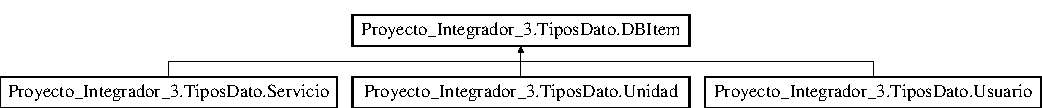
\includegraphics[height=1.430396cm]{db/d99/class_proyecto___integrador__3_1_1_tipos_dato_1_1_d_b_item}
\end{center}
\end{figure}
\subsection*{Métodos públicos}
\begin{DoxyCompactItemize}
\item 
virtual bool \hyperlink{class_proyecto___integrador__3_1_1_tipos_dato_1_1_d_b_item_ab88d7eef0fa58d7d5fdf40039867dd6e}{is\-Added} ()
\begin{DoxyCompactList}\small\item\em Determina si esta instancia esta agregada a la base de datos. \end{DoxyCompactList}\end{DoxyCompactItemize}


\subsection{Descripción detallada}
Modelo abstracto de un objeto de la base de datos 



Definición en la línea 8 del archivo D\-B\-Item.\-cs.



\subsection{Documentación de las funciones miembro}
\hypertarget{class_proyecto___integrador__3_1_1_tipos_dato_1_1_d_b_item_ab88d7eef0fa58d7d5fdf40039867dd6e}{\index{Proyecto\-\_\-\-Integrador\-\_\-3\-::\-Tipos\-Dato\-::\-D\-B\-Item@{Proyecto\-\_\-\-Integrador\-\_\-3\-::\-Tipos\-Dato\-::\-D\-B\-Item}!is\-Added@{is\-Added}}
\index{is\-Added@{is\-Added}!Proyecto_Integrador_3::TiposDato::DBItem@{Proyecto\-\_\-\-Integrador\-\_\-3\-::\-Tipos\-Dato\-::\-D\-B\-Item}}
\subsubsection[{is\-Added}]{\setlength{\rightskip}{0pt plus 5cm}virtual bool Proyecto\-\_\-\-Integrador\-\_\-3.\-Tipos\-Dato.\-D\-B\-Item.\-is\-Added (
\begin{DoxyParamCaption}
{}
\end{DoxyParamCaption}
)\hspace{0.3cm}{\ttfamily [virtual]}}}\label{class_proyecto___integrador__3_1_1_tipos_dato_1_1_d_b_item_ab88d7eef0fa58d7d5fdf40039867dd6e}


Determina si esta instancia esta agregada a la base de datos. 

\begin{DoxyReturn}{Devuelve}
Verdadero si esta agregada, falso si no
\end{DoxyReturn}


Reimplementado en \hyperlink{class_proyecto___integrador__3_1_1_tipos_dato_1_1_usuario_a6ebae0d39a68af27c93fd85719bb1664}{Proyecto\-\_\-\-Integrador\-\_\-3.\-Tipos\-Dato.\-Usuario}, \hyperlink{class_proyecto___integrador__3_1_1_tipos_dato_1_1_servicio_a84ccd70aa17d65df0afff55a14faeeec}{Proyecto\-\_\-\-Integrador\-\_\-3.\-Tipos\-Dato.\-Servicio} y \hyperlink{class_proyecto___integrador__3_1_1_tipos_dato_1_1_unidad_a6566d517c25b9048021422510c544611}{Proyecto\-\_\-\-Integrador\-\_\-3.\-Tipos\-Dato.\-Unidad}.



Definición en la línea 14 del archivo D\-B\-Item.\-cs.


\begin{DoxyCode}
15         \{
16             \textcolor{keywordflow}{throw} \textcolor{keyword}{new} NotImplementedException();
17         \}
\end{DoxyCode}


La documentación para esta clase fue generada a partir del siguiente fichero\-:\begin{DoxyCompactItemize}
\item 
C\-:/\-Users/\-Yknx4/\-Documents/\-Visual Studio 2012/\-Projects/\-Proyecto Integrador 3/\-Proyecto Integrador 3/\-Tipos\-Dato/\hyperlink{_d_b_item_8cs}{D\-B\-Item.\-cs}\end{DoxyCompactItemize}

\hypertarget{class_proyecto___integrador__3_1_1_d_b_managers_1_1_d_b_manager_3_01_t_01_4}{\section{Referencia de la plantilla de la Clase Proyecto\-\_\-\-Integrador\-\_\-3.\-D\-B\-Managers.\-D\-B\-Manager$<$ T $>$}
\label{class_proyecto___integrador__3_1_1_d_b_managers_1_1_d_b_manager_3_01_t_01_4}\index{Proyecto\-\_\-\-Integrador\-\_\-3.\-D\-B\-Managers.\-D\-B\-Manager$<$ T $>$@{Proyecto\-\_\-\-Integrador\-\_\-3.\-D\-B\-Managers.\-D\-B\-Manager$<$ T $>$}}
}
Diagrama de herencias de Proyecto\-\_\-\-Integrador\-\_\-3.\-D\-B\-Managers.\-D\-B\-Manager$<$ T $>$\begin{figure}[H]
\begin{center}
\leavevmode
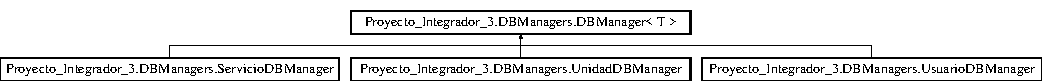
\includegraphics[height=1.075889cm]{d7/d0e/class_proyecto___integrador__3_1_1_d_b_managers_1_1_d_b_manager_3_01_t_01_4}
\end{center}
\end{figure}
\subsection*{Métodos públicos}
\begin{DoxyCompactItemize}
\item 
abstract void \hyperlink{class_proyecto___integrador__3_1_1_d_b_managers_1_1_d_b_manager_3_01_t_01_4_a820a55f3ee3c7fde31b121f3f3ea6179}{Add\-To\-D\-B} ()
\item 
abstract void \hyperlink{class_proyecto___integrador__3_1_1_d_b_managers_1_1_d_b_manager_3_01_t_01_4_a7830332e065723c1799d5804fd202dd1}{Add\-To\-Dataset} ()
\item 
abstract void \hyperlink{class_proyecto___integrador__3_1_1_d_b_managers_1_1_d_b_manager_3_01_t_01_4_aecafeb72fd4ce55d76c16c804e38dae8}{Update\-D\-B\-From\-Dataset} ()
\item 
virtual void \hyperlink{class_proyecto___integrador__3_1_1_d_b_managers_1_1_d_b_manager_3_01_t_01_4_a49ea2a7bfa58a2c536fefa4d60d488d2}{item\-Modified} (object sender, System.\-Component\-Model.\-Property\-Changed\-Event\-Args e)
\item 
abstract void \hyperlink{class_proyecto___integrador__3_1_1_d_b_managers_1_1_d_b_manager_3_01_t_01_4_a0cd8914cf3417e3df2f9d580fdb48aca}{modificar\-Dato} ()
\item 
virtual bool \hyperlink{class_proyecto___integrador__3_1_1_d_b_managers_1_1_d_b_manager_3_01_t_01_4_a436cb08914ca84122f9019a59485589a}{Remove\-From\-D\-B} ()
\item 
void \hyperlink{class_proyecto___integrador__3_1_1_d_b_managers_1_1_d_b_manager_3_01_t_01_4_a2d552a5e547efd19924ca4a96f685a56}{set\-Item} (T Input)
\item 
void \hyperlink{class_proyecto___integrador__3_1_1_d_b_managers_1_1_d_b_manager_3_01_t_01_4_ad5d7f99a4a5783514bad64ba8894e1ea}{Clear} ()
\end{DoxyCompactItemize}
\subsection*{Métodos protegidos}
\begin{DoxyCompactItemize}
\item 
\hyperlink{class_proyecto___integrador__3_1_1_d_b_managers_1_1_d_b_manager_3_01_t_01_4_afc677f4083b556311e37ad8a42cb8dd8}{D\-B\-Manager} (\hyperlink{class_proyecto___integrador__3_1_1_d_b_managers}{D\-B\-Managers} sender)
\item 
bool \hyperlink{class_proyecto___integrador__3_1_1_d_b_managers_1_1_d_b_manager_3_01_t_01_4_add66e324cef43fd10b491bc697fa60b5}{Active} ()
\end{DoxyCompactItemize}
\subsection*{Atributos protegidos}
\begin{DoxyCompactItemize}
\item 
\hyperlink{class_proyecto___integrador__3_1_1_d_b_managers}{D\-B\-Managers} \hyperlink{class_proyecto___integrador__3_1_1_d_b_managers_1_1_d_b_manager_3_01_t_01_4_a06315e75298c8f2fd46f32dc7c9a80b2}{Parent}
\item 
T \hyperlink{class_proyecto___integrador__3_1_1_d_b_managers_1_1_d_b_manager_3_01_t_01_4_a3b67ae3b5b3b9c3793d56c1407d7dcff}{held\-Item}
\end{DoxyCompactItemize}
\subsection*{Propiedades}
\begin{DoxyCompactItemize}
\item 
string \hyperlink{class_proyecto___integrador__3_1_1_d_b_managers_1_1_d_b_manager_3_01_t_01_4_a6e5caaed2ee1a4d067dfbf5aaa1b1fa8}{Error}\hspace{0.3cm}{\ttfamily  \mbox{[}get, set\mbox{]}}
\end{DoxyCompactItemize}
\subsection*{Atributos privados}
\begin{DoxyCompactItemize}
\item 
string \hyperlink{class_proyecto___integrador__3_1_1_d_b_managers_1_1_d_b_manager_3_01_t_01_4_a72ee684c84a301ba5a3c48f863bc950f}{\-\_\-error}
\end{DoxyCompactItemize}


\subsection{Descripción detallada}


Definición en la línea 7 del archivo D\-B\-Manager.\-cs.



\subsection{Documentación del constructor y destructor}
\hypertarget{class_proyecto___integrador__3_1_1_d_b_managers_1_1_d_b_manager_3_01_t_01_4_afc677f4083b556311e37ad8a42cb8dd8}{\index{Proyecto\-\_\-\-Integrador\-\_\-3\-::\-D\-B\-Managers\-::\-D\-B\-Manager$<$ T $>$@{Proyecto\-\_\-\-Integrador\-\_\-3\-::\-D\-B\-Managers\-::\-D\-B\-Manager$<$ T $>$}!D\-B\-Manager@{D\-B\-Manager}}
\index{D\-B\-Manager@{D\-B\-Manager}!Proyecto_Integrador_3::DBManagers::DBManager< T >@{Proyecto\-\_\-\-Integrador\-\_\-3\-::\-D\-B\-Managers\-::\-D\-B\-Manager$<$ T $>$}}
\subsubsection[{D\-B\-Manager}]{\setlength{\rightskip}{0pt plus 5cm}Proyecto\-\_\-\-Integrador\-\_\-3.\-D\-B\-Managers.\-D\-B\-Manager$<$ T $>$.D\-B\-Manager (
\begin{DoxyParamCaption}
\item[{{\bf D\-B\-Managers}}]{sender}
\end{DoxyParamCaption}
)\hspace{0.3cm}{\ttfamily [protected]}}}\label{class_proyecto___integrador__3_1_1_d_b_managers_1_1_d_b_manager_3_01_t_01_4_afc677f4083b556311e37ad8a42cb8dd8}


Definición en la línea 9 del archivo D\-B\-Manager.\-cs.


\begin{DoxyCode}
10             \{
11                 this.\hyperlink{class_proyecto___integrador__3_1_1_d_b_managers_1_1_d_b_manager_3_01_t_01_4_a06315e75298c8f2fd46f32dc7c9a80b2}{Parent} = sender;
12             \}
\end{DoxyCode}


\subsection{Documentación de las funciones miembro}
\hypertarget{class_proyecto___integrador__3_1_1_d_b_managers_1_1_d_b_manager_3_01_t_01_4_add66e324cef43fd10b491bc697fa60b5}{\index{Proyecto\-\_\-\-Integrador\-\_\-3\-::\-D\-B\-Managers\-::\-D\-B\-Manager$<$ T $>$@{Proyecto\-\_\-\-Integrador\-\_\-3\-::\-D\-B\-Managers\-::\-D\-B\-Manager$<$ T $>$}!Active@{Active}}
\index{Active@{Active}!Proyecto_Integrador_3::DBManagers::DBManager< T >@{Proyecto\-\_\-\-Integrador\-\_\-3\-::\-D\-B\-Managers\-::\-D\-B\-Manager$<$ T $>$}}
\subsubsection[{Active}]{\setlength{\rightskip}{0pt plus 5cm}bool Proyecto\-\_\-\-Integrador\-\_\-3.\-D\-B\-Managers.\-D\-B\-Manager$<$ T $>$.Active (
\begin{DoxyParamCaption}
{}
\end{DoxyParamCaption}
)\hspace{0.3cm}{\ttfamily [protected]}}}\label{class_proyecto___integrador__3_1_1_d_b_managers_1_1_d_b_manager_3_01_t_01_4_add66e324cef43fd10b491bc697fa60b5}


Definición en la línea 48 del archivo D\-B\-Manager.\-cs.


\begin{DoxyCode}
49             \{
50                 \textcolor{keywordflow}{if} (\hyperlink{class_proyecto___integrador__3_1_1_d_b_managers_1_1_d_b_manager_3_01_t_01_4_a3b67ae3b5b3b9c3793d56c1407d7dcff}{heldItem} == null) \textcolor{keywordflow}{return} \textcolor{keyword}{false};
51                 \textcolor{keywordflow}{return} \textcolor{keyword}{true};
52             \}
\end{DoxyCode}
\hypertarget{class_proyecto___integrador__3_1_1_d_b_managers_1_1_d_b_manager_3_01_t_01_4_a7830332e065723c1799d5804fd202dd1}{\index{Proyecto\-\_\-\-Integrador\-\_\-3\-::\-D\-B\-Managers\-::\-D\-B\-Manager$<$ T $>$@{Proyecto\-\_\-\-Integrador\-\_\-3\-::\-D\-B\-Managers\-::\-D\-B\-Manager$<$ T $>$}!Add\-To\-Dataset@{Add\-To\-Dataset}}
\index{Add\-To\-Dataset@{Add\-To\-Dataset}!Proyecto_Integrador_3::DBManagers::DBManager< T >@{Proyecto\-\_\-\-Integrador\-\_\-3\-::\-D\-B\-Managers\-::\-D\-B\-Manager$<$ T $>$}}
\subsubsection[{Add\-To\-Dataset}]{\setlength{\rightskip}{0pt plus 5cm}abstract void Proyecto\-\_\-\-Integrador\-\_\-3.\-D\-B\-Managers.\-D\-B\-Manager$<$ T $>$.Add\-To\-Dataset (
\begin{DoxyParamCaption}
{}
\end{DoxyParamCaption}
)\hspace{0.3cm}{\ttfamily [pure virtual]}}}\label{class_proyecto___integrador__3_1_1_d_b_managers_1_1_d_b_manager_3_01_t_01_4_a7830332e065723c1799d5804fd202dd1}


Implementado en \hyperlink{class_proyecto___integrador__3_1_1_d_b_managers_1_1_usuario_d_b_manager_a54c2d949592f354143fa7b7429ce1938}{Proyecto\-\_\-\-Integrador\-\_\-3.\-D\-B\-Managers.\-Usuario\-D\-B\-Manager}, \hyperlink{class_proyecto___integrador__3_1_1_d_b_managers_1_1_unidad_d_b_manager_aedd457fc6ac509e785ef85c448ceb04c}{Proyecto\-\_\-\-Integrador\-\_\-3.\-D\-B\-Managers.\-Unidad\-D\-B\-Manager} y \hyperlink{class_proyecto___integrador__3_1_1_d_b_managers_1_1_servicio_d_b_manager_a6da7980b7551fb67526270a28b7e3d35}{Proyecto\-\_\-\-Integrador\-\_\-3.\-D\-B\-Managers.\-Servicio\-D\-B\-Manager}.

\hypertarget{class_proyecto___integrador__3_1_1_d_b_managers_1_1_d_b_manager_3_01_t_01_4_a820a55f3ee3c7fde31b121f3f3ea6179}{\index{Proyecto\-\_\-\-Integrador\-\_\-3\-::\-D\-B\-Managers\-::\-D\-B\-Manager$<$ T $>$@{Proyecto\-\_\-\-Integrador\-\_\-3\-::\-D\-B\-Managers\-::\-D\-B\-Manager$<$ T $>$}!Add\-To\-D\-B@{Add\-To\-D\-B}}
\index{Add\-To\-D\-B@{Add\-To\-D\-B}!Proyecto_Integrador_3::DBManagers::DBManager< T >@{Proyecto\-\_\-\-Integrador\-\_\-3\-::\-D\-B\-Managers\-::\-D\-B\-Manager$<$ T $>$}}
\subsubsection[{Add\-To\-D\-B}]{\setlength{\rightskip}{0pt plus 5cm}abstract void Proyecto\-\_\-\-Integrador\-\_\-3.\-D\-B\-Managers.\-D\-B\-Manager$<$ T $>$.Add\-To\-D\-B (
\begin{DoxyParamCaption}
{}
\end{DoxyParamCaption}
)\hspace{0.3cm}{\ttfamily [pure virtual]}}}\label{class_proyecto___integrador__3_1_1_d_b_managers_1_1_d_b_manager_3_01_t_01_4_a820a55f3ee3c7fde31b121f3f3ea6179}


Implementado en \hyperlink{class_proyecto___integrador__3_1_1_d_b_managers_1_1_unidad_d_b_manager_a7ab559a77f8d4a8f7f3677331b062dc8}{Proyecto\-\_\-\-Integrador\-\_\-3.\-D\-B\-Managers.\-Unidad\-D\-B\-Manager}, \hyperlink{class_proyecto___integrador__3_1_1_d_b_managers_1_1_servicio_d_b_manager_abbc936c9fa59cae0fc302c44e6389876}{Proyecto\-\_\-\-Integrador\-\_\-3.\-D\-B\-Managers.\-Servicio\-D\-B\-Manager} y \hyperlink{class_proyecto___integrador__3_1_1_d_b_managers_1_1_usuario_d_b_manager_a40976ea1cf23f128217f7379f175d504}{Proyecto\-\_\-\-Integrador\-\_\-3.\-D\-B\-Managers.\-Usuario\-D\-B\-Manager}.

\hypertarget{class_proyecto___integrador__3_1_1_d_b_managers_1_1_d_b_manager_3_01_t_01_4_ad5d7f99a4a5783514bad64ba8894e1ea}{\index{Proyecto\-\_\-\-Integrador\-\_\-3\-::\-D\-B\-Managers\-::\-D\-B\-Manager$<$ T $>$@{Proyecto\-\_\-\-Integrador\-\_\-3\-::\-D\-B\-Managers\-::\-D\-B\-Manager$<$ T $>$}!Clear@{Clear}}
\index{Clear@{Clear}!Proyecto_Integrador_3::DBManagers::DBManager< T >@{Proyecto\-\_\-\-Integrador\-\_\-3\-::\-D\-B\-Managers\-::\-D\-B\-Manager$<$ T $>$}}
\subsubsection[{Clear}]{\setlength{\rightskip}{0pt plus 5cm}void Proyecto\-\_\-\-Integrador\-\_\-3.\-D\-B\-Managers.\-D\-B\-Manager$<$ T $>$.Clear (
\begin{DoxyParamCaption}
{}
\end{DoxyParamCaption}
)}}\label{class_proyecto___integrador__3_1_1_d_b_managers_1_1_d_b_manager_3_01_t_01_4_ad5d7f99a4a5783514bad64ba8894e1ea}


Definición en la línea 43 del archivo D\-B\-Manager.\-cs.


\begin{DoxyCode}
44             \{
45                 \hyperlink{class_proyecto___integrador__3_1_1_d_b_managers_1_1_d_b_manager_3_01_t_01_4_a3b67ae3b5b3b9c3793d56c1407d7dcff}{heldItem} = \textcolor{keywordflow}{default}(T);
46             \}
\end{DoxyCode}
\hypertarget{class_proyecto___integrador__3_1_1_d_b_managers_1_1_d_b_manager_3_01_t_01_4_a49ea2a7bfa58a2c536fefa4d60d488d2}{\index{Proyecto\-\_\-\-Integrador\-\_\-3\-::\-D\-B\-Managers\-::\-D\-B\-Manager$<$ T $>$@{Proyecto\-\_\-\-Integrador\-\_\-3\-::\-D\-B\-Managers\-::\-D\-B\-Manager$<$ T $>$}!item\-Modified@{item\-Modified}}
\index{item\-Modified@{item\-Modified}!Proyecto_Integrador_3::DBManagers::DBManager< T >@{Proyecto\-\_\-\-Integrador\-\_\-3\-::\-D\-B\-Managers\-::\-D\-B\-Manager$<$ T $>$}}
\subsubsection[{item\-Modified}]{\setlength{\rightskip}{0pt plus 5cm}virtual void Proyecto\-\_\-\-Integrador\-\_\-3.\-D\-B\-Managers.\-D\-B\-Manager$<$ T $>$.item\-Modified (
\begin{DoxyParamCaption}
\item[{object}]{sender, }
\item[{System.\-Component\-Model.\-Property\-Changed\-Event\-Args}]{e}
\end{DoxyParamCaption}
)\hspace{0.3cm}{\ttfamily [virtual]}}}\label{class_proyecto___integrador__3_1_1_d_b_managers_1_1_d_b_manager_3_01_t_01_4_a49ea2a7bfa58a2c536fefa4d60d488d2}


Definición en la línea 20 del archivo D\-B\-Manager.\-cs.


\begin{DoxyCode}
21             \{
22                 \hyperlink{class_proyecto___integrador__3_1_1_d_b_managers_1_1_d_b_manager_3_01_t_01_4_a2d552a5e547efd19924ca4a96f685a56}{setItem}((T)sender);
23             \}
\end{DoxyCode}
\hypertarget{class_proyecto___integrador__3_1_1_d_b_managers_1_1_d_b_manager_3_01_t_01_4_a0cd8914cf3417e3df2f9d580fdb48aca}{\index{Proyecto\-\_\-\-Integrador\-\_\-3\-::\-D\-B\-Managers\-::\-D\-B\-Manager$<$ T $>$@{Proyecto\-\_\-\-Integrador\-\_\-3\-::\-D\-B\-Managers\-::\-D\-B\-Manager$<$ T $>$}!modificar\-Dato@{modificar\-Dato}}
\index{modificar\-Dato@{modificar\-Dato}!Proyecto_Integrador_3::DBManagers::DBManager< T >@{Proyecto\-\_\-\-Integrador\-\_\-3\-::\-D\-B\-Managers\-::\-D\-B\-Manager$<$ T $>$}}
\subsubsection[{modificar\-Dato}]{\setlength{\rightskip}{0pt plus 5cm}abstract void Proyecto\-\_\-\-Integrador\-\_\-3.\-D\-B\-Managers.\-D\-B\-Manager$<$ T $>$.modificar\-Dato (
\begin{DoxyParamCaption}
{}
\end{DoxyParamCaption}
)\hspace{0.3cm}{\ttfamily [pure virtual]}}}\label{class_proyecto___integrador__3_1_1_d_b_managers_1_1_d_b_manager_3_01_t_01_4_a0cd8914cf3417e3df2f9d580fdb48aca}


Implementado en \hyperlink{class_proyecto___integrador__3_1_1_d_b_managers_1_1_usuario_d_b_manager_a367d61aaac1f426d93800be80159eadd}{Proyecto\-\_\-\-Integrador\-\_\-3.\-D\-B\-Managers.\-Usuario\-D\-B\-Manager}, \hyperlink{class_proyecto___integrador__3_1_1_d_b_managers_1_1_unidad_d_b_manager_a06b95538d895923d0a3b780fdde83e06}{Proyecto\-\_\-\-Integrador\-\_\-3.\-D\-B\-Managers.\-Unidad\-D\-B\-Manager} y \hyperlink{class_proyecto___integrador__3_1_1_d_b_managers_1_1_servicio_d_b_manager_a903bee917e813d25c2e9a4ad87281db4}{Proyecto\-\_\-\-Integrador\-\_\-3.\-D\-B\-Managers.\-Servicio\-D\-B\-Manager}.

\hypertarget{class_proyecto___integrador__3_1_1_d_b_managers_1_1_d_b_manager_3_01_t_01_4_a436cb08914ca84122f9019a59485589a}{\index{Proyecto\-\_\-\-Integrador\-\_\-3\-::\-D\-B\-Managers\-::\-D\-B\-Manager$<$ T $>$@{Proyecto\-\_\-\-Integrador\-\_\-3\-::\-D\-B\-Managers\-::\-D\-B\-Manager$<$ T $>$}!Remove\-From\-D\-B@{Remove\-From\-D\-B}}
\index{Remove\-From\-D\-B@{Remove\-From\-D\-B}!Proyecto_Integrador_3::DBManagers::DBManager< T >@{Proyecto\-\_\-\-Integrador\-\_\-3\-::\-D\-B\-Managers\-::\-D\-B\-Manager$<$ T $>$}}
\subsubsection[{Remove\-From\-D\-B}]{\setlength{\rightskip}{0pt plus 5cm}virtual bool Proyecto\-\_\-\-Integrador\-\_\-3.\-D\-B\-Managers.\-D\-B\-Manager$<$ T $>$.Remove\-From\-D\-B (
\begin{DoxyParamCaption}
{}
\end{DoxyParamCaption}
)\hspace{0.3cm}{\ttfamily [virtual]}}}\label{class_proyecto___integrador__3_1_1_d_b_managers_1_1_d_b_manager_3_01_t_01_4_a436cb08914ca84122f9019a59485589a}


Definición en la línea 27 del archivo D\-B\-Manager.\-cs.


\begin{DoxyCode}
28             \{
29                 \textcolor{keywordflow}{throw} \textcolor{keyword}{new} NotImplementedException();
30             \}
\end{DoxyCode}
\hypertarget{class_proyecto___integrador__3_1_1_d_b_managers_1_1_d_b_manager_3_01_t_01_4_a2d552a5e547efd19924ca4a96f685a56}{\index{Proyecto\-\_\-\-Integrador\-\_\-3\-::\-D\-B\-Managers\-::\-D\-B\-Manager$<$ T $>$@{Proyecto\-\_\-\-Integrador\-\_\-3\-::\-D\-B\-Managers\-::\-D\-B\-Manager$<$ T $>$}!set\-Item@{set\-Item}}
\index{set\-Item@{set\-Item}!Proyecto_Integrador_3::DBManagers::DBManager< T >@{Proyecto\-\_\-\-Integrador\-\_\-3\-::\-D\-B\-Managers\-::\-D\-B\-Manager$<$ T $>$}}
\subsubsection[{set\-Item}]{\setlength{\rightskip}{0pt plus 5cm}void Proyecto\-\_\-\-Integrador\-\_\-3.\-D\-B\-Managers.\-D\-B\-Manager$<$ T $>$.set\-Item (
\begin{DoxyParamCaption}
\item[{T}]{Input}
\end{DoxyParamCaption}
)}}\label{class_proyecto___integrador__3_1_1_d_b_managers_1_1_d_b_manager_3_01_t_01_4_a2d552a5e547efd19924ca4a96f685a56}


Definición en la línea 38 del archivo D\-B\-Manager.\-cs.


\begin{DoxyCode}
39             \{
40                 \hyperlink{class_proyecto___integrador__3_1_1_d_b_managers_1_1_d_b_manager_3_01_t_01_4_a3b67ae3b5b3b9c3793d56c1407d7dcff}{heldItem} = Input;
41             \}
\end{DoxyCode}
\hypertarget{class_proyecto___integrador__3_1_1_d_b_managers_1_1_d_b_manager_3_01_t_01_4_aecafeb72fd4ce55d76c16c804e38dae8}{\index{Proyecto\-\_\-\-Integrador\-\_\-3\-::\-D\-B\-Managers\-::\-D\-B\-Manager$<$ T $>$@{Proyecto\-\_\-\-Integrador\-\_\-3\-::\-D\-B\-Managers\-::\-D\-B\-Manager$<$ T $>$}!Update\-D\-B\-From\-Dataset@{Update\-D\-B\-From\-Dataset}}
\index{Update\-D\-B\-From\-Dataset@{Update\-D\-B\-From\-Dataset}!Proyecto_Integrador_3::DBManagers::DBManager< T >@{Proyecto\-\_\-\-Integrador\-\_\-3\-::\-D\-B\-Managers\-::\-D\-B\-Manager$<$ T $>$}}
\subsubsection[{Update\-D\-B\-From\-Dataset}]{\setlength{\rightskip}{0pt plus 5cm}abstract void Proyecto\-\_\-\-Integrador\-\_\-3.\-D\-B\-Managers.\-D\-B\-Manager$<$ T $>$.Update\-D\-B\-From\-Dataset (
\begin{DoxyParamCaption}
{}
\end{DoxyParamCaption}
)\hspace{0.3cm}{\ttfamily [pure virtual]}}}\label{class_proyecto___integrador__3_1_1_d_b_managers_1_1_d_b_manager_3_01_t_01_4_aecafeb72fd4ce55d76c16c804e38dae8}


Implementado en \hyperlink{class_proyecto___integrador__3_1_1_d_b_managers_1_1_usuario_d_b_manager_af38f312f9fd5a10d9a8d7d43e880d555}{Proyecto\-\_\-\-Integrador\-\_\-3.\-D\-B\-Managers.\-Usuario\-D\-B\-Manager}, \hyperlink{class_proyecto___integrador__3_1_1_d_b_managers_1_1_unidad_d_b_manager_a4161021ecc4778c81b88592d0cb1d23b}{Proyecto\-\_\-\-Integrador\-\_\-3.\-D\-B\-Managers.\-Unidad\-D\-B\-Manager} y \hyperlink{class_proyecto___integrador__3_1_1_d_b_managers_1_1_servicio_d_b_manager_a2ff2e7d573e60b876f4b183defc8675f}{Proyecto\-\_\-\-Integrador\-\_\-3.\-D\-B\-Managers.\-Servicio\-D\-B\-Manager}.



\subsection{Documentación de los datos miembro}
\hypertarget{class_proyecto___integrador__3_1_1_d_b_managers_1_1_d_b_manager_3_01_t_01_4_a72ee684c84a301ba5a3c48f863bc950f}{\index{Proyecto\-\_\-\-Integrador\-\_\-3\-::\-D\-B\-Managers\-::\-D\-B\-Manager$<$ T $>$@{Proyecto\-\_\-\-Integrador\-\_\-3\-::\-D\-B\-Managers\-::\-D\-B\-Manager$<$ T $>$}!\-\_\-error@{\-\_\-error}}
\index{\-\_\-error@{\-\_\-error}!Proyecto_Integrador_3::DBManagers::DBManager< T >@{Proyecto\-\_\-\-Integrador\-\_\-3\-::\-D\-B\-Managers\-::\-D\-B\-Manager$<$ T $>$}}
\subsubsection[{\-\_\-error}]{\setlength{\rightskip}{0pt plus 5cm}string Proyecto\-\_\-\-Integrador\-\_\-3.\-D\-B\-Managers.\-D\-B\-Manager$<$ T $>$.\-\_\-error\hspace{0.3cm}{\ttfamily [private]}}}\label{class_proyecto___integrador__3_1_1_d_b_managers_1_1_d_b_manager_3_01_t_01_4_a72ee684c84a301ba5a3c48f863bc950f}


Definición en la línea 54 del archivo D\-B\-Manager.\-cs.

\hypertarget{class_proyecto___integrador__3_1_1_d_b_managers_1_1_d_b_manager_3_01_t_01_4_a3b67ae3b5b3b9c3793d56c1407d7dcff}{\index{Proyecto\-\_\-\-Integrador\-\_\-3\-::\-D\-B\-Managers\-::\-D\-B\-Manager$<$ T $>$@{Proyecto\-\_\-\-Integrador\-\_\-3\-::\-D\-B\-Managers\-::\-D\-B\-Manager$<$ T $>$}!held\-Item@{held\-Item}}
\index{held\-Item@{held\-Item}!Proyecto_Integrador_3::DBManagers::DBManager< T >@{Proyecto\-\_\-\-Integrador\-\_\-3\-::\-D\-B\-Managers\-::\-D\-B\-Manager$<$ T $>$}}
\subsubsection[{held\-Item}]{\setlength{\rightskip}{0pt plus 5cm}T Proyecto\-\_\-\-Integrador\-\_\-3.\-D\-B\-Managers.\-D\-B\-Manager$<$ T $>$.held\-Item\hspace{0.3cm}{\ttfamily [protected]}}}\label{class_proyecto___integrador__3_1_1_d_b_managers_1_1_d_b_manager_3_01_t_01_4_a3b67ae3b5b3b9c3793d56c1407d7dcff}


Definición en la línea 34 del archivo D\-B\-Manager.\-cs.

\hypertarget{class_proyecto___integrador__3_1_1_d_b_managers_1_1_d_b_manager_3_01_t_01_4_a06315e75298c8f2fd46f32dc7c9a80b2}{\index{Proyecto\-\_\-\-Integrador\-\_\-3\-::\-D\-B\-Managers\-::\-D\-B\-Manager$<$ T $>$@{Proyecto\-\_\-\-Integrador\-\_\-3\-::\-D\-B\-Managers\-::\-D\-B\-Manager$<$ T $>$}!Parent@{Parent}}
\index{Parent@{Parent}!Proyecto_Integrador_3::DBManagers::DBManager< T >@{Proyecto\-\_\-\-Integrador\-\_\-3\-::\-D\-B\-Managers\-::\-D\-B\-Manager$<$ T $>$}}
\subsubsection[{Parent}]{\setlength{\rightskip}{0pt plus 5cm}{\bf D\-B\-Managers} Proyecto\-\_\-\-Integrador\-\_\-3.\-D\-B\-Managers.\-D\-B\-Manager$<$ T $>$.Parent\hspace{0.3cm}{\ttfamily [protected]}}}\label{class_proyecto___integrador__3_1_1_d_b_managers_1_1_d_b_manager_3_01_t_01_4_a06315e75298c8f2fd46f32dc7c9a80b2}


Definición en la línea 32 del archivo D\-B\-Manager.\-cs.



\subsection{Documentación de propiedades}
\hypertarget{class_proyecto___integrador__3_1_1_d_b_managers_1_1_d_b_manager_3_01_t_01_4_a6e5caaed2ee1a4d067dfbf5aaa1b1fa8}{\index{Proyecto\-\_\-\-Integrador\-\_\-3\-::\-D\-B\-Managers\-::\-D\-B\-Manager$<$ T $>$@{Proyecto\-\_\-\-Integrador\-\_\-3\-::\-D\-B\-Managers\-::\-D\-B\-Manager$<$ T $>$}!Error@{Error}}
\index{Error@{Error}!Proyecto_Integrador_3::DBManagers::DBManager< T >@{Proyecto\-\_\-\-Integrador\-\_\-3\-::\-D\-B\-Managers\-::\-D\-B\-Manager$<$ T $>$}}
\subsubsection[{Error}]{\setlength{\rightskip}{0pt plus 5cm}string Proyecto\-\_\-\-Integrador\-\_\-3.\-D\-B\-Managers.\-D\-B\-Manager$<$ T $>$.Error\hspace{0.3cm}{\ttfamily [get]}, {\ttfamily [set]}}}\label{class_proyecto___integrador__3_1_1_d_b_managers_1_1_d_b_manager_3_01_t_01_4_a6e5caaed2ee1a4d067dfbf5aaa1b1fa8}


Definición en la línea 56 del archivo D\-B\-Manager.\-cs.



La documentación para esta clase fue generada a partir del siguiente fichero\-:\begin{DoxyCompactItemize}
\item 
C\-:/\-Users/\-Yknx4/\-Documents/\-Visual Studio 2012/\-Projects/\-Proyecto Integrador 3/\-Proyecto Integrador 3/\-Manejadores/\hyperlink{_d_b_manager_8cs}{D\-B\-Manager.\-cs}\end{DoxyCompactItemize}

\hypertarget{class_proyecto___integrador__3_1_1_d_b_managers}{\section{Referencia de la Clase Proyecto\-\_\-\-Integrador\-\_\-3.\-D\-B\-Managers}
\label{class_proyecto___integrador__3_1_1_d_b_managers}\index{Proyecto\-\_\-\-Integrador\-\_\-3.\-D\-B\-Managers@{Proyecto\-\_\-\-Integrador\-\_\-3.\-D\-B\-Managers}}
}


Realiza la lógica de la interacción con la base de datos  


\subsection*{Clases}
\begin{DoxyCompactItemize}
\item 
class \hyperlink{class_proyecto___integrador__3_1_1_d_b_managers_1_1_d_b_manager_3_01_t_01_4}{D\-B\-Manager$<$ T $>$}
\item 
class \hyperlink{class_proyecto___integrador__3_1_1_d_b_managers_1_1_servicio_d_b_manager}{Servicio\-D\-B\-Manager}
\begin{DoxyCompactList}\small\item\em Maneja los accesos a la base de datos de los Servicios \end{DoxyCompactList}\item 
class \hyperlink{class_proyecto___integrador__3_1_1_d_b_managers_1_1_servicios_populator}{Servicios\-Populator}
\begin{DoxyCompactList}\small\item\em Llena las listas de Servicios \end{DoxyCompactList}\item 
class \hyperlink{class_proyecto___integrador__3_1_1_d_b_managers_1_1_unidad_d_b_manager}{Unidad\-D\-B\-Manager}
\begin{DoxyCompactList}\small\item\em Maneja los accesos a la base de datos de las Unidades \end{DoxyCompactList}\item 
class \hyperlink{class_proyecto___integrador__3_1_1_d_b_managers_1_1_unidad_populator}{Unidad\-Populator}
\item 
class \hyperlink{class_proyecto___integrador__3_1_1_d_b_managers_1_1_usuario_d_b_manager}{Usuario\-D\-B\-Manager}
\begin{DoxyCompactList}\small\item\em Maneja los accesos a la base de datos de los Usuarios \end{DoxyCompactList}\item 
class \hyperlink{class_proyecto___integrador__3_1_1_d_b_managers_1_1_usuarios_populator}{Usuarios\-Populator}
\begin{DoxyCompactList}\small\item\em Llena las listas de Usuarios \end{DoxyCompactList}\end{DoxyCompactItemize}
\subsection*{Métodos públicos}
\begin{DoxyCompactItemize}
\item 
void \hyperlink{class_proyecto___integrador__3_1_1_d_b_managers_ab1d4758dc7cca9b54a51d63ec6e6589b}{Refresh} ()
\item 
\hyperlink{class_proyecto___integrador__3_1_1_d_b_managers_ae18ebe2d8858254a6077fbb32842f2ab}{D\-B\-Managers} ()
\item 
void \hyperlink{class_proyecto___integrador__3_1_1_d_b_managers_a2af606713823aab2912dd18c719aeb48}{Clear} ()
\item 
void \hyperlink{class_proyecto___integrador__3_1_1_d_b_managers_a3766dfbef6eb8494cf1fd9e28a135bd7}{Fill} ()
\item 
void \hyperlink{class_proyecto___integrador__3_1_1_d_b_managers_a27dce97a7e23ba80a56b545ccfeb73ee}{Fill\-Usuarios} ()
\item 
void \hyperlink{class_proyecto___integrador__3_1_1_d_b_managers_af664570cb8838acf770610b1d14eecea}{Fill\-Unidades} ()
\item 
void \hyperlink{class_proyecto___integrador__3_1_1_d_b_managers_af60e768a1ec8417d606d3e718d6a22d5}{Fill\-Servicios} ()
\item 
void \hyperlink{class_proyecto___integrador__3_1_1_d_b_managers_a51daa549b13a4bc2b6f12c0960286bae}{Clear\-Usuarios} ()
\item 
void \hyperlink{class_proyecto___integrador__3_1_1_d_b_managers_aa0c3c65b856fa31237f75b6a74194d03}{Clear\-Unidades} ()
\item 
void \hyperlink{class_proyecto___integrador__3_1_1_d_b_managers_ac449742a91d365aa025fd4f10db38604}{Clear\-Servicios} ()
\end{DoxyCompactItemize}
\subsection*{Atributos públicos}
\begin{DoxyCompactItemize}
\item 
string \hyperlink{class_proyecto___integrador__3_1_1_d_b_managers_aecf2d3981e87f16c1e3a60c7913931a8}{Last\-Message} = \char`\"{}\char`\"{}
\end{DoxyCompactItemize}
\subsection*{Atributos protegidos}
\begin{DoxyCompactItemize}
\item 
\hyperlink{class_proyecto___integrador__3_1_1ds_servicios}{ds\-Servicios} \hyperlink{class_proyecto___integrador__3_1_1_d_b_managers_a6b992d164f75898c6f9717fd5b839fa4}{mds\-Servicios} = new \hyperlink{class_proyecto___integrador__3_1_1ds_servicios}{ds\-Servicios}()
\item 
\hyperlink{class_proyecto___integrador__3_1_1ds_servicios_table_adapters_1_1_servicios_table_adapter}{Servicios\-Table\-Adapter} \hyperlink{class_proyecto___integrador__3_1_1_d_b_managers_a1f9e67f272910356a732a882769c8dac}{m\-Servicios\-Table\-Adapter} = new \hyperlink{class_proyecto___integrador__3_1_1ds_servicios_table_adapters_1_1_servicios_table_adapter}{Servicios\-Table\-Adapter}()
\item 
\hyperlink{class_proyecto___integrador__3_1_1ds_unidad}{ds\-Unidad} \hyperlink{class_proyecto___integrador__3_1_1_d_b_managers_a0e58571e4517bd6ac941eae32baaf978}{mds\-Unidades} = new \hyperlink{class_proyecto___integrador__3_1_1ds_unidad}{ds\-Unidad}()
\item 
\hyperlink{class_proyecto___integrador__3_1_1ds_unidad_table_adapters_1_1_unidad_table_adapter}{Unidad\-Table\-Adapter} \hyperlink{class_proyecto___integrador__3_1_1_d_b_managers_a5d36d244f440437683f2b0cd30720ac5}{m\-Unidadles\-Table\-Adapter} = new \hyperlink{class_proyecto___integrador__3_1_1ds_unidad_table_adapters_1_1_unidad_table_adapter}{Unidad\-Table\-Adapter}()
\item 
\hyperlink{class_proyecto___integrador__3_1_1ds_usuarios}{ds\-Usuarios} \hyperlink{class_proyecto___integrador__3_1_1_d_b_managers_a19d87c9abf32e08e2969847a008eb195}{mds\-Usuarios} = new \hyperlink{class_proyecto___integrador__3_1_1ds_usuarios}{ds\-Usuarios}()
\item 
\hyperlink{class_proyecto___integrador__3_1_1ds_usuarios_table_adapters_1_1_usuarios_table_adapter}{Usuarios\-Table\-Adapter} \hyperlink{class_proyecto___integrador__3_1_1_d_b_managers_a8830e1bb507bcd7277966a4aabe3e830}{m\-Usuarios\-Table\-Adapter} = new \hyperlink{class_proyecto___integrador__3_1_1ds_usuarios_table_adapters_1_1_usuarios_table_adapter}{Usuarios\-Table\-Adapter}()
\end{DoxyCompactItemize}
\subsection*{Propiedades}
\begin{DoxyCompactItemize}
\item 
bool \hyperlink{class_proyecto___integrador__3_1_1_d_b_managers_ae2d3910ba77a23556e32c950f9886644}{Are\-Usuarios\-Filled}\hspace{0.3cm}{\ttfamily  \mbox{[}get, set\mbox{]}}
\item 
bool \hyperlink{class_proyecto___integrador__3_1_1_d_b_managers_a440e953b052887695a270a359fc9051c}{Are\-Unidades\-Filled}\hspace{0.3cm}{\ttfamily  \mbox{[}get, set\mbox{]}}
\item 
bool \hyperlink{class_proyecto___integrador__3_1_1_d_b_managers_ae2ca731707c9af5dce9d66be4744cf64}{Are\-Servicios\-Filled}\hspace{0.3cm}{\ttfamily  \mbox{[}get, set\mbox{]}}
\end{DoxyCompactItemize}


\subsection{Descripción detallada}
Realiza la lógica de la interacción con la base de datos 

Clase base para la interacción con la base de datos.

Definición en la línea 6 del archivo D\-B\-Managers.\-cs.



\subsection{Documentación del constructor y destructor}
\hypertarget{class_proyecto___integrador__3_1_1_d_b_managers_ae18ebe2d8858254a6077fbb32842f2ab}{\index{Proyecto\-\_\-\-Integrador\-\_\-3\-::\-D\-B\-Managers@{Proyecto\-\_\-\-Integrador\-\_\-3\-::\-D\-B\-Managers}!D\-B\-Managers@{D\-B\-Managers}}
\index{D\-B\-Managers@{D\-B\-Managers}!Proyecto_Integrador_3::DBManagers@{Proyecto\-\_\-\-Integrador\-\_\-3\-::\-D\-B\-Managers}}
\subsubsection[{D\-B\-Managers}]{\setlength{\rightskip}{0pt plus 5cm}Proyecto\-\_\-\-Integrador\-\_\-3.\-D\-B\-Managers.\-D\-B\-Managers (
\begin{DoxyParamCaption}
{}
\end{DoxyParamCaption}
)}}\label{class_proyecto___integrador__3_1_1_d_b_managers_ae18ebe2d8858254a6077fbb32842f2ab}


Definición en la línea 16 del archivo D\-B\-Managers.\-cs.


\begin{DoxyCode}
17         \{
18             \hyperlink{class_proyecto___integrador__3_1_1_d_b_managers_ae2d3910ba77a23556e32c950f9886644}{AreUsuariosFilled} = \textcolor{keyword}{false};
19             \hyperlink{class_proyecto___integrador__3_1_1_d_b_managers_ae2ca731707c9af5dce9d66be4744cf64}{AreServiciosFilled} = \textcolor{keyword}{false};
20             \hyperlink{class_proyecto___integrador__3_1_1_d_b_managers_a440e953b052887695a270a359fc9051c}{AreUnidadesFilled} = \textcolor{keyword}{false};
21         \}
\end{DoxyCode}


\subsection{Documentación de las funciones miembro}
\hypertarget{class_proyecto___integrador__3_1_1_d_b_managers_a2af606713823aab2912dd18c719aeb48}{\index{Proyecto\-\_\-\-Integrador\-\_\-3\-::\-D\-B\-Managers@{Proyecto\-\_\-\-Integrador\-\_\-3\-::\-D\-B\-Managers}!Clear@{Clear}}
\index{Clear@{Clear}!Proyecto_Integrador_3::DBManagers@{Proyecto\-\_\-\-Integrador\-\_\-3\-::\-D\-B\-Managers}}
\subsubsection[{Clear}]{\setlength{\rightskip}{0pt plus 5cm}void Proyecto\-\_\-\-Integrador\-\_\-3.\-D\-B\-Managers.\-Clear (
\begin{DoxyParamCaption}
{}
\end{DoxyParamCaption}
)}}\label{class_proyecto___integrador__3_1_1_d_b_managers_a2af606713823aab2912dd18c719aeb48}


Definición en la línea 23 del archivo D\-B\-Managers.\-cs.


\begin{DoxyCode}
24         \{
25             \hyperlink{class_proyecto___integrador__3_1_1_d_b_managers_a51daa549b13a4bc2b6f12c0960286bae}{ClearUsuarios}();
26             \hyperlink{class_proyecto___integrador__3_1_1_d_b_managers_aa0c3c65b856fa31237f75b6a74194d03}{ClearUnidades}();
27             \hyperlink{class_proyecto___integrador__3_1_1_d_b_managers_ac449742a91d365aa025fd4f10db38604}{ClearServicios}();
28         \}
\end{DoxyCode}
\hypertarget{class_proyecto___integrador__3_1_1_d_b_managers_ac449742a91d365aa025fd4f10db38604}{\index{Proyecto\-\_\-\-Integrador\-\_\-3\-::\-D\-B\-Managers@{Proyecto\-\_\-\-Integrador\-\_\-3\-::\-D\-B\-Managers}!Clear\-Servicios@{Clear\-Servicios}}
\index{Clear\-Servicios@{Clear\-Servicios}!Proyecto_Integrador_3::DBManagers@{Proyecto\-\_\-\-Integrador\-\_\-3\-::\-D\-B\-Managers}}
\subsubsection[{Clear\-Servicios}]{\setlength{\rightskip}{0pt plus 5cm}void Proyecto\-\_\-\-Integrador\-\_\-3.\-D\-B\-Managers.\-Clear\-Servicios (
\begin{DoxyParamCaption}
{}
\end{DoxyParamCaption}
)}}\label{class_proyecto___integrador__3_1_1_d_b_managers_ac449742a91d365aa025fd4f10db38604}


Definición en la línea 85 del archivo D\-B\-Managers.\-cs.


\begin{DoxyCode}
86         \{
87             \hyperlink{class_proyecto___integrador__3_1_1_d_b_managers_a6b992d164f75898c6f9717fd5b839fa4}{mdsServicios}.Clear();
88             \hyperlink{class_proyecto___integrador__3_1_1_d_b_managers_ae2ca731707c9af5dce9d66be4744cf64}{AreServiciosFilled} = \textcolor{keyword}{false};
89         \}
\end{DoxyCode}
\hypertarget{class_proyecto___integrador__3_1_1_d_b_managers_aa0c3c65b856fa31237f75b6a74194d03}{\index{Proyecto\-\_\-\-Integrador\-\_\-3\-::\-D\-B\-Managers@{Proyecto\-\_\-\-Integrador\-\_\-3\-::\-D\-B\-Managers}!Clear\-Unidades@{Clear\-Unidades}}
\index{Clear\-Unidades@{Clear\-Unidades}!Proyecto_Integrador_3::DBManagers@{Proyecto\-\_\-\-Integrador\-\_\-3\-::\-D\-B\-Managers}}
\subsubsection[{Clear\-Unidades}]{\setlength{\rightskip}{0pt plus 5cm}void Proyecto\-\_\-\-Integrador\-\_\-3.\-D\-B\-Managers.\-Clear\-Unidades (
\begin{DoxyParamCaption}
{}
\end{DoxyParamCaption}
)}}\label{class_proyecto___integrador__3_1_1_d_b_managers_aa0c3c65b856fa31237f75b6a74194d03}


Definición en la línea 79 del archivo D\-B\-Managers.\-cs.


\begin{DoxyCode}
80         \{
81             \hyperlink{class_proyecto___integrador__3_1_1_d_b_managers_a0e58571e4517bd6ac941eae32baaf978}{mdsUnidades}.Clear();
82             \hyperlink{class_proyecto___integrador__3_1_1_d_b_managers_a440e953b052887695a270a359fc9051c}{AreUnidadesFilled} = \textcolor{keyword}{false};
83         \}
\end{DoxyCode}
\hypertarget{class_proyecto___integrador__3_1_1_d_b_managers_a51daa549b13a4bc2b6f12c0960286bae}{\index{Proyecto\-\_\-\-Integrador\-\_\-3\-::\-D\-B\-Managers@{Proyecto\-\_\-\-Integrador\-\_\-3\-::\-D\-B\-Managers}!Clear\-Usuarios@{Clear\-Usuarios}}
\index{Clear\-Usuarios@{Clear\-Usuarios}!Proyecto_Integrador_3::DBManagers@{Proyecto\-\_\-\-Integrador\-\_\-3\-::\-D\-B\-Managers}}
\subsubsection[{Clear\-Usuarios}]{\setlength{\rightskip}{0pt plus 5cm}void Proyecto\-\_\-\-Integrador\-\_\-3.\-D\-B\-Managers.\-Clear\-Usuarios (
\begin{DoxyParamCaption}
{}
\end{DoxyParamCaption}
)}}\label{class_proyecto___integrador__3_1_1_d_b_managers_a51daa549b13a4bc2b6f12c0960286bae}


Definición en la línea 73 del archivo D\-B\-Managers.\-cs.


\begin{DoxyCode}
74         \{
75             \hyperlink{class_proyecto___integrador__3_1_1_d_b_managers_a19d87c9abf32e08e2969847a008eb195}{mdsUsuarios}.Clear();
76             \hyperlink{class_proyecto___integrador__3_1_1_d_b_managers_ae2d3910ba77a23556e32c950f9886644}{AreUsuariosFilled} = \textcolor{keyword}{false};
77         \}
\end{DoxyCode}
\hypertarget{class_proyecto___integrador__3_1_1_d_b_managers_a3766dfbef6eb8494cf1fd9e28a135bd7}{\index{Proyecto\-\_\-\-Integrador\-\_\-3\-::\-D\-B\-Managers@{Proyecto\-\_\-\-Integrador\-\_\-3\-::\-D\-B\-Managers}!Fill@{Fill}}
\index{Fill@{Fill}!Proyecto_Integrador_3::DBManagers@{Proyecto\-\_\-\-Integrador\-\_\-3\-::\-D\-B\-Managers}}
\subsubsection[{Fill}]{\setlength{\rightskip}{0pt plus 5cm}void Proyecto\-\_\-\-Integrador\-\_\-3.\-D\-B\-Managers.\-Fill (
\begin{DoxyParamCaption}
{}
\end{DoxyParamCaption}
)}}\label{class_proyecto___integrador__3_1_1_d_b_managers_a3766dfbef6eb8494cf1fd9e28a135bd7}


Definición en la línea 30 del archivo D\-B\-Managers.\-cs.


\begin{DoxyCode}
31         \{
32             \hyperlink{class_proyecto___integrador__3_1_1_d_b_managers_af664570cb8838acf770610b1d14eecea}{FillUnidades}();
33             \hyperlink{class_proyecto___integrador__3_1_1_d_b_managers_a27dce97a7e23ba80a56b545ccfeb73ee}{FillUsuarios}();
34             \hyperlink{class_proyecto___integrador__3_1_1_d_b_managers_af60e768a1ec8417d606d3e718d6a22d5}{FillServicios}();
35         \}
\end{DoxyCode}
\hypertarget{class_proyecto___integrador__3_1_1_d_b_managers_af60e768a1ec8417d606d3e718d6a22d5}{\index{Proyecto\-\_\-\-Integrador\-\_\-3\-::\-D\-B\-Managers@{Proyecto\-\_\-\-Integrador\-\_\-3\-::\-D\-B\-Managers}!Fill\-Servicios@{Fill\-Servicios}}
\index{Fill\-Servicios@{Fill\-Servicios}!Proyecto_Integrador_3::DBManagers@{Proyecto\-\_\-\-Integrador\-\_\-3\-::\-D\-B\-Managers}}
\subsubsection[{Fill\-Servicios}]{\setlength{\rightskip}{0pt plus 5cm}void Proyecto\-\_\-\-Integrador\-\_\-3.\-D\-B\-Managers.\-Fill\-Servicios (
\begin{DoxyParamCaption}
{}
\end{DoxyParamCaption}
)}}\label{class_proyecto___integrador__3_1_1_d_b_managers_af60e768a1ec8417d606d3e718d6a22d5}


Definición en la línea 67 del archivo D\-B\-Managers.\-cs.


\begin{DoxyCode}
68         \{
69             \hyperlink{class_proyecto___integrador__3_1_1_d_b_managers_a1f9e67f272910356a732a882769c8dac}{mServiciosTableAdapter}.Fill(\hyperlink{class_proyecto___integrador__3_1_1_d_b_managers_a6b992d164f75898c6f9717fd5b839fa4}{mdsServicios}.
      \hyperlink{class_proyecto___integrador__3_1_1ds_servicios_a03c1b1284ccc9c2b139d6102da34f6e9}{Servicios});
70             \hyperlink{class_proyecto___integrador__3_1_1_d_b_managers_ae2ca731707c9af5dce9d66be4744cf64}{AreServiciosFilled} = \textcolor{keyword}{true};
71         \}
\end{DoxyCode}
\hypertarget{class_proyecto___integrador__3_1_1_d_b_managers_af664570cb8838acf770610b1d14eecea}{\index{Proyecto\-\_\-\-Integrador\-\_\-3\-::\-D\-B\-Managers@{Proyecto\-\_\-\-Integrador\-\_\-3\-::\-D\-B\-Managers}!Fill\-Unidades@{Fill\-Unidades}}
\index{Fill\-Unidades@{Fill\-Unidades}!Proyecto_Integrador_3::DBManagers@{Proyecto\-\_\-\-Integrador\-\_\-3\-::\-D\-B\-Managers}}
\subsubsection[{Fill\-Unidades}]{\setlength{\rightskip}{0pt plus 5cm}void Proyecto\-\_\-\-Integrador\-\_\-3.\-D\-B\-Managers.\-Fill\-Unidades (
\begin{DoxyParamCaption}
{}
\end{DoxyParamCaption}
)}}\label{class_proyecto___integrador__3_1_1_d_b_managers_af664570cb8838acf770610b1d14eecea}


Definición en la línea 61 del archivo D\-B\-Managers.\-cs.


\begin{DoxyCode}
62         \{
63             \hyperlink{class_proyecto___integrador__3_1_1_d_b_managers_a5d36d244f440437683f2b0cd30720ac5}{mUnidadlesTableAdapter}.Fill(\hyperlink{class_proyecto___integrador__3_1_1_d_b_managers_a0e58571e4517bd6ac941eae32baaf978}{mdsUnidades}.
      \hyperlink{class_proyecto___integrador__3_1_1ds_unidad_a78a56c4320f0067f020ea95490bdf195}{Unidad});
64             \hyperlink{class_proyecto___integrador__3_1_1_d_b_managers_a440e953b052887695a270a359fc9051c}{AreUnidadesFilled} = \textcolor{keyword}{true};
65         \}
\end{DoxyCode}
\hypertarget{class_proyecto___integrador__3_1_1_d_b_managers_a27dce97a7e23ba80a56b545ccfeb73ee}{\index{Proyecto\-\_\-\-Integrador\-\_\-3\-::\-D\-B\-Managers@{Proyecto\-\_\-\-Integrador\-\_\-3\-::\-D\-B\-Managers}!Fill\-Usuarios@{Fill\-Usuarios}}
\index{Fill\-Usuarios@{Fill\-Usuarios}!Proyecto_Integrador_3::DBManagers@{Proyecto\-\_\-\-Integrador\-\_\-3\-::\-D\-B\-Managers}}
\subsubsection[{Fill\-Usuarios}]{\setlength{\rightskip}{0pt plus 5cm}void Proyecto\-\_\-\-Integrador\-\_\-3.\-D\-B\-Managers.\-Fill\-Usuarios (
\begin{DoxyParamCaption}
{}
\end{DoxyParamCaption}
)}}\label{class_proyecto___integrador__3_1_1_d_b_managers_a27dce97a7e23ba80a56b545ccfeb73ee}


Definición en la línea 55 del archivo D\-B\-Managers.\-cs.


\begin{DoxyCode}
56         \{
57             \hyperlink{class_proyecto___integrador__3_1_1_d_b_managers_a8830e1bb507bcd7277966a4aabe3e830}{mUsuariosTableAdapter}.Fill(\hyperlink{class_proyecto___integrador__3_1_1_d_b_managers_a19d87c9abf32e08e2969847a008eb195}{mdsUsuarios}.
      \hyperlink{class_proyecto___integrador__3_1_1ds_usuarios_a79d1cfd31914c2c5cfda39b62381478b}{Usuarios});
58             \hyperlink{class_proyecto___integrador__3_1_1_d_b_managers_ae2d3910ba77a23556e32c950f9886644}{AreUsuariosFilled} = \textcolor{keyword}{true};
59         \}
\end{DoxyCode}
\hypertarget{class_proyecto___integrador__3_1_1_d_b_managers_ab1d4758dc7cca9b54a51d63ec6e6589b}{\index{Proyecto\-\_\-\-Integrador\-\_\-3\-::\-D\-B\-Managers@{Proyecto\-\_\-\-Integrador\-\_\-3\-::\-D\-B\-Managers}!Refresh@{Refresh}}
\index{Refresh@{Refresh}!Proyecto_Integrador_3::DBManagers@{Proyecto\-\_\-\-Integrador\-\_\-3\-::\-D\-B\-Managers}}
\subsubsection[{Refresh}]{\setlength{\rightskip}{0pt plus 5cm}void Proyecto\-\_\-\-Integrador\-\_\-3.\-D\-B\-Managers.\-Refresh (
\begin{DoxyParamCaption}
{}
\end{DoxyParamCaption}
)}}\label{class_proyecto___integrador__3_1_1_d_b_managers_ab1d4758dc7cca9b54a51d63ec6e6589b}


Definición en la línea 10 del archivo D\-B\-Managers.\-cs.


\begin{DoxyCode}
11         \{
12             \hyperlink{class_proyecto___integrador__3_1_1_d_b_managers_a2af606713823aab2912dd18c719aeb48}{Clear}();
13             \hyperlink{class_proyecto___integrador__3_1_1_d_b_managers_a3766dfbef6eb8494cf1fd9e28a135bd7}{Fill}();
14         \}
\end{DoxyCode}


\subsection{Documentación de los datos miembro}
\hypertarget{class_proyecto___integrador__3_1_1_d_b_managers_aecf2d3981e87f16c1e3a60c7913931a8}{\index{Proyecto\-\_\-\-Integrador\-\_\-3\-::\-D\-B\-Managers@{Proyecto\-\_\-\-Integrador\-\_\-3\-::\-D\-B\-Managers}!Last\-Message@{Last\-Message}}
\index{Last\-Message@{Last\-Message}!Proyecto_Integrador_3::DBManagers@{Proyecto\-\_\-\-Integrador\-\_\-3\-::\-D\-B\-Managers}}
\subsubsection[{Last\-Message}]{\setlength{\rightskip}{0pt plus 5cm}string Proyecto\-\_\-\-Integrador\-\_\-3.\-D\-B\-Managers.\-Last\-Message = \char`\"{}\char`\"{}}}\label{class_proyecto___integrador__3_1_1_d_b_managers_aecf2d3981e87f16c1e3a60c7913931a8}


Definición en la línea 8 del archivo D\-B\-Managers.\-cs.

\hypertarget{class_proyecto___integrador__3_1_1_d_b_managers_a6b992d164f75898c6f9717fd5b839fa4}{\index{Proyecto\-\_\-\-Integrador\-\_\-3\-::\-D\-B\-Managers@{Proyecto\-\_\-\-Integrador\-\_\-3\-::\-D\-B\-Managers}!mds\-Servicios@{mds\-Servicios}}
\index{mds\-Servicios@{mds\-Servicios}!Proyecto_Integrador_3::DBManagers@{Proyecto\-\_\-\-Integrador\-\_\-3\-::\-D\-B\-Managers}}
\subsubsection[{mds\-Servicios}]{\setlength{\rightskip}{0pt plus 5cm}{\bf ds\-Servicios} Proyecto\-\_\-\-Integrador\-\_\-3.\-D\-B\-Managers.\-mds\-Servicios = new {\bf ds\-Servicios}()\hspace{0.3cm}{\ttfamily [protected]}}}\label{class_proyecto___integrador__3_1_1_d_b_managers_a6b992d164f75898c6f9717fd5b839fa4}


Definición en la línea 10 del archivo Servicio\-D\-B\-Manager.\-cs.

\hypertarget{class_proyecto___integrador__3_1_1_d_b_managers_a0e58571e4517bd6ac941eae32baaf978}{\index{Proyecto\-\_\-\-Integrador\-\_\-3\-::\-D\-B\-Managers@{Proyecto\-\_\-\-Integrador\-\_\-3\-::\-D\-B\-Managers}!mds\-Unidades@{mds\-Unidades}}
\index{mds\-Unidades@{mds\-Unidades}!Proyecto_Integrador_3::DBManagers@{Proyecto\-\_\-\-Integrador\-\_\-3\-::\-D\-B\-Managers}}
\subsubsection[{mds\-Unidades}]{\setlength{\rightskip}{0pt plus 5cm}{\bf ds\-Unidad} Proyecto\-\_\-\-Integrador\-\_\-3.\-D\-B\-Managers.\-mds\-Unidades = new {\bf ds\-Unidad}()\hspace{0.3cm}{\ttfamily [protected]}}}\label{class_proyecto___integrador__3_1_1_d_b_managers_a0e58571e4517bd6ac941eae32baaf978}


Definición en la línea 11 del archivo Unidad\-D\-B\-Manager.\-cs.

\hypertarget{class_proyecto___integrador__3_1_1_d_b_managers_a19d87c9abf32e08e2969847a008eb195}{\index{Proyecto\-\_\-\-Integrador\-\_\-3\-::\-D\-B\-Managers@{Proyecto\-\_\-\-Integrador\-\_\-3\-::\-D\-B\-Managers}!mds\-Usuarios@{mds\-Usuarios}}
\index{mds\-Usuarios@{mds\-Usuarios}!Proyecto_Integrador_3::DBManagers@{Proyecto\-\_\-\-Integrador\-\_\-3\-::\-D\-B\-Managers}}
\subsubsection[{mds\-Usuarios}]{\setlength{\rightskip}{0pt plus 5cm}{\bf ds\-Usuarios} Proyecto\-\_\-\-Integrador\-\_\-3.\-D\-B\-Managers.\-mds\-Usuarios = new {\bf ds\-Usuarios}()\hspace{0.3cm}{\ttfamily [protected]}}}\label{class_proyecto___integrador__3_1_1_d_b_managers_a19d87c9abf32e08e2969847a008eb195}


Definición en la línea 10 del archivo Usuario\-D\-B\-Manager.\-cs.

\hypertarget{class_proyecto___integrador__3_1_1_d_b_managers_a1f9e67f272910356a732a882769c8dac}{\index{Proyecto\-\_\-\-Integrador\-\_\-3\-::\-D\-B\-Managers@{Proyecto\-\_\-\-Integrador\-\_\-3\-::\-D\-B\-Managers}!m\-Servicios\-Table\-Adapter@{m\-Servicios\-Table\-Adapter}}
\index{m\-Servicios\-Table\-Adapter@{m\-Servicios\-Table\-Adapter}!Proyecto_Integrador_3::DBManagers@{Proyecto\-\_\-\-Integrador\-\_\-3\-::\-D\-B\-Managers}}
\subsubsection[{m\-Servicios\-Table\-Adapter}]{\setlength{\rightskip}{0pt plus 5cm}{\bf Servicios\-Table\-Adapter} Proyecto\-\_\-\-Integrador\-\_\-3.\-D\-B\-Managers.\-m\-Servicios\-Table\-Adapter = new {\bf Servicios\-Table\-Adapter}()\hspace{0.3cm}{\ttfamily [protected]}}}\label{class_proyecto___integrador__3_1_1_d_b_managers_a1f9e67f272910356a732a882769c8dac}


Definición en la línea 11 del archivo Servicio\-D\-B\-Manager.\-cs.

\hypertarget{class_proyecto___integrador__3_1_1_d_b_managers_a5d36d244f440437683f2b0cd30720ac5}{\index{Proyecto\-\_\-\-Integrador\-\_\-3\-::\-D\-B\-Managers@{Proyecto\-\_\-\-Integrador\-\_\-3\-::\-D\-B\-Managers}!m\-Unidadles\-Table\-Adapter@{m\-Unidadles\-Table\-Adapter}}
\index{m\-Unidadles\-Table\-Adapter@{m\-Unidadles\-Table\-Adapter}!Proyecto_Integrador_3::DBManagers@{Proyecto\-\_\-\-Integrador\-\_\-3\-::\-D\-B\-Managers}}
\subsubsection[{m\-Unidadles\-Table\-Adapter}]{\setlength{\rightskip}{0pt plus 5cm}{\bf Unidad\-Table\-Adapter} Proyecto\-\_\-\-Integrador\-\_\-3.\-D\-B\-Managers.\-m\-Unidadles\-Table\-Adapter = new {\bf Unidad\-Table\-Adapter}()\hspace{0.3cm}{\ttfamily [protected]}}}\label{class_proyecto___integrador__3_1_1_d_b_managers_a5d36d244f440437683f2b0cd30720ac5}


Definición en la línea 12 del archivo Unidad\-D\-B\-Manager.\-cs.

\hypertarget{class_proyecto___integrador__3_1_1_d_b_managers_a8830e1bb507bcd7277966a4aabe3e830}{\index{Proyecto\-\_\-\-Integrador\-\_\-3\-::\-D\-B\-Managers@{Proyecto\-\_\-\-Integrador\-\_\-3\-::\-D\-B\-Managers}!m\-Usuarios\-Table\-Adapter@{m\-Usuarios\-Table\-Adapter}}
\index{m\-Usuarios\-Table\-Adapter@{m\-Usuarios\-Table\-Adapter}!Proyecto_Integrador_3::DBManagers@{Proyecto\-\_\-\-Integrador\-\_\-3\-::\-D\-B\-Managers}}
\subsubsection[{m\-Usuarios\-Table\-Adapter}]{\setlength{\rightskip}{0pt plus 5cm}{\bf Usuarios\-Table\-Adapter} Proyecto\-\_\-\-Integrador\-\_\-3.\-D\-B\-Managers.\-m\-Usuarios\-Table\-Adapter = new {\bf Usuarios\-Table\-Adapter}()\hspace{0.3cm}{\ttfamily [protected]}}}\label{class_proyecto___integrador__3_1_1_d_b_managers_a8830e1bb507bcd7277966a4aabe3e830}


Definición en la línea 11 del archivo Usuario\-D\-B\-Manager.\-cs.



\subsection{Documentación de propiedades}
\hypertarget{class_proyecto___integrador__3_1_1_d_b_managers_ae2ca731707c9af5dce9d66be4744cf64}{\index{Proyecto\-\_\-\-Integrador\-\_\-3\-::\-D\-B\-Managers@{Proyecto\-\_\-\-Integrador\-\_\-3\-::\-D\-B\-Managers}!Are\-Servicios\-Filled@{Are\-Servicios\-Filled}}
\index{Are\-Servicios\-Filled@{Are\-Servicios\-Filled}!Proyecto_Integrador_3::DBManagers@{Proyecto\-\_\-\-Integrador\-\_\-3\-::\-D\-B\-Managers}}
\subsubsection[{Are\-Servicios\-Filled}]{\setlength{\rightskip}{0pt plus 5cm}bool Proyecto\-\_\-\-Integrador\-\_\-3.\-D\-B\-Managers.\-Are\-Servicios\-Filled\hspace{0.3cm}{\ttfamily [get]}, {\ttfamily [set]}}}\label{class_proyecto___integrador__3_1_1_d_b_managers_ae2ca731707c9af5dce9d66be4744cf64}


Definición en la línea 50 del archivo D\-B\-Managers.\-cs.

\hypertarget{class_proyecto___integrador__3_1_1_d_b_managers_a440e953b052887695a270a359fc9051c}{\index{Proyecto\-\_\-\-Integrador\-\_\-3\-::\-D\-B\-Managers@{Proyecto\-\_\-\-Integrador\-\_\-3\-::\-D\-B\-Managers}!Are\-Unidades\-Filled@{Are\-Unidades\-Filled}}
\index{Are\-Unidades\-Filled@{Are\-Unidades\-Filled}!Proyecto_Integrador_3::DBManagers@{Proyecto\-\_\-\-Integrador\-\_\-3\-::\-D\-B\-Managers}}
\subsubsection[{Are\-Unidades\-Filled}]{\setlength{\rightskip}{0pt plus 5cm}bool Proyecto\-\_\-\-Integrador\-\_\-3.\-D\-B\-Managers.\-Are\-Unidades\-Filled\hspace{0.3cm}{\ttfamily [get]}, {\ttfamily [set]}}}\label{class_proyecto___integrador__3_1_1_d_b_managers_a440e953b052887695a270a359fc9051c}


Definición en la línea 44 del archivo D\-B\-Managers.\-cs.

\hypertarget{class_proyecto___integrador__3_1_1_d_b_managers_ae2d3910ba77a23556e32c950f9886644}{\index{Proyecto\-\_\-\-Integrador\-\_\-3\-::\-D\-B\-Managers@{Proyecto\-\_\-\-Integrador\-\_\-3\-::\-D\-B\-Managers}!Are\-Usuarios\-Filled@{Are\-Usuarios\-Filled}}
\index{Are\-Usuarios\-Filled@{Are\-Usuarios\-Filled}!Proyecto_Integrador_3::DBManagers@{Proyecto\-\_\-\-Integrador\-\_\-3\-::\-D\-B\-Managers}}
\subsubsection[{Are\-Usuarios\-Filled}]{\setlength{\rightskip}{0pt plus 5cm}bool Proyecto\-\_\-\-Integrador\-\_\-3.\-D\-B\-Managers.\-Are\-Usuarios\-Filled\hspace{0.3cm}{\ttfamily [get]}, {\ttfamily [set]}}}\label{class_proyecto___integrador__3_1_1_d_b_managers_ae2d3910ba77a23556e32c950f9886644}


Definición en la línea 38 del archivo D\-B\-Managers.\-cs.



La documentación para esta clase fue generada a partir de los siguientes ficheros\-:\begin{DoxyCompactItemize}
\item 
C\-:/\-Users/\-Yknx4/\-Documents/\-Visual Studio 2012/\-Projects/\-Proyecto Integrador 3/\-Proyecto Integrador 3/\hyperlink{_d_b_managers_8cs}{D\-B\-Managers.\-cs}\item 
C\-:/\-Users/\-Yknx4/\-Documents/\-Visual Studio 2012/\-Projects/\-Proyecto Integrador 3/\-Proyecto Integrador 3/\-Manejadores/\hyperlink{_servicio_d_b_manager_8cs}{Servicio\-D\-B\-Manager.\-cs}\item 
C\-:/\-Users/\-Yknx4/\-Documents/\-Visual Studio 2012/\-Projects/\-Proyecto Integrador 3/\-Proyecto Integrador 3/\-Manejadores/\hyperlink{_unidad_d_b_manager_8cs}{Unidad\-D\-B\-Manager.\-cs}\item 
C\-:/\-Users/\-Yknx4/\-Documents/\-Visual Studio 2012/\-Projects/\-Proyecto Integrador 3/\-Proyecto Integrador 3/\-Manejadores/\hyperlink{_usuario_d_b_manager_8cs}{Usuario\-D\-B\-Manager.\-cs}\end{DoxyCompactItemize}

\hypertarget{struct_proyecto___integrador__3_1_1_tipos_dato_1_1_usuario_1_1_domicilio}{\section{Referencia de la Estructura Proyecto\-\_\-\-Integrador\-\_\-3.\-Tipos\-Dato.\-Usuario.\-Domicilio}
\label{struct_proyecto___integrador__3_1_1_tipos_dato_1_1_usuario_1_1_domicilio}\index{Proyecto\-\_\-\-Integrador\-\_\-3.\-Tipos\-Dato.\-Usuario.\-Domicilio@{Proyecto\-\_\-\-Integrador\-\_\-3.\-Tipos\-Dato.\-Usuario.\-Domicilio}}
}
\subsection*{Propiedades}
\begin{DoxyCompactItemize}
\item 
string \hyperlink{struct_proyecto___integrador__3_1_1_tipos_dato_1_1_usuario_1_1_domicilio_ac7f639c760a904e006a4ea6a3db05dff}{Calle}\hspace{0.3cm}{\ttfamily  \mbox{[}get, set\mbox{]}}
\item 
int \hyperlink{struct_proyecto___integrador__3_1_1_tipos_dato_1_1_usuario_1_1_domicilio_a31d02de9239bc44c3da8022fc36419e1}{Numero}\hspace{0.3cm}{\ttfamily  \mbox{[}get, set\mbox{]}}
\item 
string \hyperlink{struct_proyecto___integrador__3_1_1_tipos_dato_1_1_usuario_1_1_domicilio_a0782bc382740439c8b0340518e7ad972}{Colonia}\hspace{0.3cm}{\ttfamily  \mbox{[}get, set\mbox{]}}
\item 
short \hyperlink{struct_proyecto___integrador__3_1_1_tipos_dato_1_1_usuario_1_1_domicilio_a909e9dfc0615a13937e6c4134dca57c5}{Municipio}\hspace{0.3cm}{\ttfamily  \mbox{[}get, set\mbox{]}}
\end{DoxyCompactItemize}


\subsection{Descripción detallada}


Definición en la línea 11 del archivo Usuario.\-cs.



\subsection{Documentación de propiedades}
\hypertarget{struct_proyecto___integrador__3_1_1_tipos_dato_1_1_usuario_1_1_domicilio_ac7f639c760a904e006a4ea6a3db05dff}{\index{Proyecto\-\_\-\-Integrador\-\_\-3\-::\-Tipos\-Dato\-::\-Usuario\-::\-Domicilio@{Proyecto\-\_\-\-Integrador\-\_\-3\-::\-Tipos\-Dato\-::\-Usuario\-::\-Domicilio}!Calle@{Calle}}
\index{Calle@{Calle}!Proyecto_Integrador_3::TiposDato::Usuario::Domicilio@{Proyecto\-\_\-\-Integrador\-\_\-3\-::\-Tipos\-Dato\-::\-Usuario\-::\-Domicilio}}
\subsubsection[{Calle}]{\setlength{\rightskip}{0pt plus 5cm}string Proyecto\-\_\-\-Integrador\-\_\-3.\-Tipos\-Dato.\-Usuario.\-Domicilio.\-Calle\hspace{0.3cm}{\ttfamily [get]}, {\ttfamily [set]}}}\label{struct_proyecto___integrador__3_1_1_tipos_dato_1_1_usuario_1_1_domicilio_ac7f639c760a904e006a4ea6a3db05dff}


Definición en la línea 13 del archivo Usuario.\-cs.

\hypertarget{struct_proyecto___integrador__3_1_1_tipos_dato_1_1_usuario_1_1_domicilio_a0782bc382740439c8b0340518e7ad972}{\index{Proyecto\-\_\-\-Integrador\-\_\-3\-::\-Tipos\-Dato\-::\-Usuario\-::\-Domicilio@{Proyecto\-\_\-\-Integrador\-\_\-3\-::\-Tipos\-Dato\-::\-Usuario\-::\-Domicilio}!Colonia@{Colonia}}
\index{Colonia@{Colonia}!Proyecto_Integrador_3::TiposDato::Usuario::Domicilio@{Proyecto\-\_\-\-Integrador\-\_\-3\-::\-Tipos\-Dato\-::\-Usuario\-::\-Domicilio}}
\subsubsection[{Colonia}]{\setlength{\rightskip}{0pt plus 5cm}string Proyecto\-\_\-\-Integrador\-\_\-3.\-Tipos\-Dato.\-Usuario.\-Domicilio.\-Colonia\hspace{0.3cm}{\ttfamily [get]}, {\ttfamily [set]}}}\label{struct_proyecto___integrador__3_1_1_tipos_dato_1_1_usuario_1_1_domicilio_a0782bc382740439c8b0340518e7ad972}


Definición en la línea 17 del archivo Usuario.\-cs.

\hypertarget{struct_proyecto___integrador__3_1_1_tipos_dato_1_1_usuario_1_1_domicilio_a909e9dfc0615a13937e6c4134dca57c5}{\index{Proyecto\-\_\-\-Integrador\-\_\-3\-::\-Tipos\-Dato\-::\-Usuario\-::\-Domicilio@{Proyecto\-\_\-\-Integrador\-\_\-3\-::\-Tipos\-Dato\-::\-Usuario\-::\-Domicilio}!Municipio@{Municipio}}
\index{Municipio@{Municipio}!Proyecto_Integrador_3::TiposDato::Usuario::Domicilio@{Proyecto\-\_\-\-Integrador\-\_\-3\-::\-Tipos\-Dato\-::\-Usuario\-::\-Domicilio}}
\subsubsection[{Municipio}]{\setlength{\rightskip}{0pt plus 5cm}short Proyecto\-\_\-\-Integrador\-\_\-3.\-Tipos\-Dato.\-Usuario.\-Domicilio.\-Municipio\hspace{0.3cm}{\ttfamily [get]}, {\ttfamily [set]}}}\label{struct_proyecto___integrador__3_1_1_tipos_dato_1_1_usuario_1_1_domicilio_a909e9dfc0615a13937e6c4134dca57c5}


Definición en la línea 19 del archivo Usuario.\-cs.

\hypertarget{struct_proyecto___integrador__3_1_1_tipos_dato_1_1_usuario_1_1_domicilio_a31d02de9239bc44c3da8022fc36419e1}{\index{Proyecto\-\_\-\-Integrador\-\_\-3\-::\-Tipos\-Dato\-::\-Usuario\-::\-Domicilio@{Proyecto\-\_\-\-Integrador\-\_\-3\-::\-Tipos\-Dato\-::\-Usuario\-::\-Domicilio}!Numero@{Numero}}
\index{Numero@{Numero}!Proyecto_Integrador_3::TiposDato::Usuario::Domicilio@{Proyecto\-\_\-\-Integrador\-\_\-3\-::\-Tipos\-Dato\-::\-Usuario\-::\-Domicilio}}
\subsubsection[{Numero}]{\setlength{\rightskip}{0pt plus 5cm}int Proyecto\-\_\-\-Integrador\-\_\-3.\-Tipos\-Dato.\-Usuario.\-Domicilio.\-Numero\hspace{0.3cm}{\ttfamily [get]}, {\ttfamily [set]}}}\label{struct_proyecto___integrador__3_1_1_tipos_dato_1_1_usuario_1_1_domicilio_a31d02de9239bc44c3da8022fc36419e1}


Definición en la línea 15 del archivo Usuario.\-cs.



La documentación para esta estructura fue generada a partir del siguiente fichero\-:\begin{DoxyCompactItemize}
\item 
C\-:/\-Users/\-Yknx4/\-Documents/\-Visual Studio 2012/\-Projects/\-Proyecto Integrador 3/\-Proyecto Integrador 3/\-Tipos\-Dato/\hyperlink{_usuario_8cs}{Usuario.\-cs}\end{DoxyCompactItemize}

\hypertarget{class_proyecto___integrador__3_1_1ds_servicios}{\section{Referencia de la Clase Proyecto\-\_\-\-Integrador\-\_\-3.\-ds\-Servicios}
\label{class_proyecto___integrador__3_1_1ds_servicios}\index{Proyecto\-\_\-\-Integrador\-\_\-3.\-ds\-Servicios@{Proyecto\-\_\-\-Integrador\-\_\-3.\-ds\-Servicios}}
}


Represents a strongly typed in-\/memory cache of data.  


Diagrama de herencias de Proyecto\-\_\-\-Integrador\-\_\-3.\-ds\-Servicios\begin{figure}[H]
\begin{center}
\leavevmode
\includegraphics[height=2.000000cm]{da/d6b/class_proyecto___integrador__3_1_1ds_servicios}
\end{center}
\end{figure}
\subsection*{Clases}
\begin{DoxyCompactItemize}
\item 
class \hyperlink{class_proyecto___integrador__3_1_1ds_servicios_1_1_servicios_data_table}{Servicios\-Data\-Table}
\begin{DoxyCompactList}\small\item\em Represents the strongly named Data\-Table class. \end{DoxyCompactList}\item 
class \hyperlink{class_proyecto___integrador__3_1_1ds_servicios_1_1_servicios_row}{Servicios\-Row}
\begin{DoxyCompactList}\small\item\em Represents strongly named Data\-Row class. \end{DoxyCompactList}\item 
class \hyperlink{class_proyecto___integrador__3_1_1ds_servicios_1_1_servicios_row_change_event}{Servicios\-Row\-Change\-Event}
\begin{DoxyCompactList}\small\item\em Row event argument class /summary$>$ \end{DoxyCompactList}\end{DoxyCompactItemize}
\subsection*{Métodos públicos}
\begin{DoxyCompactItemize}
\item 
\hyperlink{class_proyecto___integrador__3_1_1ds_servicios_a0734e62bba29ca7515ed72f2aee94662}{ds\-Servicios} ()
\item 
override \\*
global\-::\-System.\-Data.\-Data\-Set \hyperlink{class_proyecto___integrador__3_1_1ds_servicios_a6925c56a7154d89ed11f16a7b45434f7}{Clone} ()
\item 
delegate void \hyperlink{class_proyecto___integrador__3_1_1ds_servicios_a12a7c95915227392e001d214be4c6c58}{Servicios\-Row\-Change\-Event\-Handler} (object sender, \hyperlink{class_proyecto___integrador__3_1_1ds_servicios_1_1_servicios_row_change_event}{Servicios\-Row\-Change\-Event} e)
\end{DoxyCompactItemize}
\subsection*{Métodos públicos estáticos}
\begin{DoxyCompactItemize}
\item 
static \\*
global\-::\-System.\-Xml.\-Schema.\-Xml\-Schema\-Complex\-Type \hyperlink{class_proyecto___integrador__3_1_1ds_servicios_a4df975c629e0d4abeb51fc99bd5d9cdd}{Get\-Typed\-Data\-Set\-Schema} (global\-::\-System.\-Xml.\-Schema.\-Xml\-Schema\-Set xs)
\end{DoxyCompactItemize}
\subsection*{Métodos protegidos}
\begin{DoxyCompactItemize}
\item 
\hyperlink{class_proyecto___integrador__3_1_1ds_servicios_a9c16aad1d299f9a0f4e8206476970c80}{ds\-Servicios} (global\-::\-System.\-Runtime.\-Serialization.\-Serialization\-Info info, global\-::\-System.\-Runtime.\-Serialization.\-Streaming\-Context context)
\item 
override void \hyperlink{class_proyecto___integrador__3_1_1ds_servicios_a0fdfd68e26fcf989dc0baaddaeb65cd6}{Initialize\-Derived\-Data\-Set} ()
\item 
override bool \hyperlink{class_proyecto___integrador__3_1_1ds_servicios_a5c968fc20f7357c59446a2359f6dff7d}{Should\-Serialize\-Tables} ()
\item 
override bool \hyperlink{class_proyecto___integrador__3_1_1ds_servicios_acb67b4c55e4372ca6319f5639640bf6e}{Should\-Serialize\-Relations} ()
\item 
override void \hyperlink{class_proyecto___integrador__3_1_1ds_servicios_ad7fe046c07204e180948c180786a41f5}{Read\-Xml\-Serializable} (global\-::\-System.\-Xml.\-Xml\-Reader reader)
\item 
override \\*
global\-::\-System.\-Xml.\-Schema.\-Xml\-Schema \hyperlink{class_proyecto___integrador__3_1_1ds_servicios_a6ae2de80ca82f7e90ee19212c90cc127}{Get\-Schema\-Serializable} ()
\end{DoxyCompactItemize}
\subsection*{Funciones del 'package'}
\begin{DoxyCompactItemize}
\item 
void \hyperlink{class_proyecto___integrador__3_1_1ds_servicios_a58f88c51e90b3494390aa1cd37635db0}{Init\-Vars} ()
\item 
void \hyperlink{class_proyecto___integrador__3_1_1ds_servicios_a1637aa2b1c235c969ae3fec848a75e2e}{Init\-Vars} (bool init\-Table)
\end{DoxyCompactItemize}
\subsection*{Propiedades}
\begin{DoxyCompactItemize}
\item 
\hyperlink{class_proyecto___integrador__3_1_1ds_servicios_1_1_servicios_data_table}{Servicios\-Data\-Table} \hyperlink{class_proyecto___integrador__3_1_1ds_servicios_a03c1b1284ccc9c2b139d6102da34f6e9}{Servicios}\hspace{0.3cm}{\ttfamily  \mbox{[}get\mbox{]}}
\item 
override \\*
global\-::\-System.\-Data.\-Schema\-Serialization\-Mode \hyperlink{class_proyecto___integrador__3_1_1ds_servicios_a062b8dfa3dfcc4aa92a8bf2d69194589}{Schema\-Serialization\-Mode}\hspace{0.3cm}{\ttfamily  \mbox{[}get, set\mbox{]}}
\item 
new \\*
global\-::\-System.\-Data.\-Data\-Table\-Collection \hyperlink{class_proyecto___integrador__3_1_1ds_servicios_a2b08d569f4f435957a1f10b46c304cb2}{Tables}\hspace{0.3cm}{\ttfamily  \mbox{[}get\mbox{]}}
\item 
new \\*
global\-::\-System.\-Data.\-Data\-Relation\-Collection \hyperlink{class_proyecto___integrador__3_1_1ds_servicios_a4a938f593d4405efc7c790a3b3a5b9d7}{Relations}\hspace{0.3cm}{\ttfamily  \mbox{[}get\mbox{]}}
\end{DoxyCompactItemize}
\subsection*{Métodos privados}
\begin{DoxyCompactItemize}
\item 
void \hyperlink{class_proyecto___integrador__3_1_1ds_servicios_a8c235d04c7e4dac9966f771f9517e5bf}{Init\-Class} ()
\item 
bool \hyperlink{class_proyecto___integrador__3_1_1ds_servicios_a207b5614ad2666dd9212ee57fd3338e2}{Should\-Serialize\-Servicios} ()
\item 
void \hyperlink{class_proyecto___integrador__3_1_1ds_servicios_ac0aff57addf6d1f24077d11c3abe845e}{Schema\-Changed} (object sender, global\-::\-System.\-Component\-Model.\-Collection\-Change\-Event\-Args e)
\end{DoxyCompactItemize}
\subsection*{Atributos privados}
\begin{DoxyCompactItemize}
\item 
\hyperlink{class_proyecto___integrador__3_1_1ds_servicios_1_1_servicios_data_table}{Servicios\-Data\-Table} \hyperlink{class_proyecto___integrador__3_1_1ds_servicios_a68ae0be2da362f71e5b2623b4ceb7380}{table\-Servicios}
\item 
global\-::\-System.\-Data.\-Schema\-Serialization\-Mode \hyperlink{class_proyecto___integrador__3_1_1ds_servicios_aa24e53512ea217f603268b7dcc69c0cf}{\-\_\-schema\-Serialization\-Mode} = global\-::\-System.\-Data.\-Schema\-Serialization\-Mode.\-Include\-Schema
\end{DoxyCompactItemize}


\subsection{Descripción detallada}
Represents a strongly typed in-\/memory cache of data. 

/summary$>$ 

Definición en la línea 25 del archivo ds\-Servicios.\-Designer.\-cs.



\subsection{Documentación del constructor y destructor}
\hypertarget{class_proyecto___integrador__3_1_1ds_servicios_a0734e62bba29ca7515ed72f2aee94662}{\index{Proyecto\-\_\-\-Integrador\-\_\-3\-::ds\-Servicios@{Proyecto\-\_\-\-Integrador\-\_\-3\-::ds\-Servicios}!ds\-Servicios@{ds\-Servicios}}
\index{ds\-Servicios@{ds\-Servicios}!Proyecto_Integrador_3::dsServicios@{Proyecto\-\_\-\-Integrador\-\_\-3\-::ds\-Servicios}}
\subsubsection[{ds\-Servicios}]{\setlength{\rightskip}{0pt plus 5cm}Proyecto\-\_\-\-Integrador\-\_\-3.\-ds\-Servicios.\-ds\-Servicios (
\begin{DoxyParamCaption}
{}
\end{DoxyParamCaption}
)\hspace{0.3cm}{\ttfamily [inline]}}}\label{class_proyecto___integrador__3_1_1ds_servicios_a0734e62bba29ca7515ed72f2aee94662}


Definición en la línea 33 del archivo ds\-Servicios.\-Designer.\-cs.


\begin{DoxyCode}
33                              \{
34             this.BeginInit();
35             this.\hyperlink{class_proyecto___integrador__3_1_1ds_servicios_a8c235d04c7e4dac9966f771f9517e5bf}{InitClass}();
36             global::System.ComponentModel.CollectionChangeEventHandler schemaChangedHandler = \textcolor{keyword}{new} 
      global::System.ComponentModel.CollectionChangeEventHandler(this.\hyperlink{class_proyecto___integrador__3_1_1ds_servicios_ac0aff57addf6d1f24077d11c3abe845e}{SchemaChanged});
37             base.Tables.CollectionChanged += schemaChangedHandler;
38             base.Relations.CollectionChanged += schemaChangedHandler;
39             this.EndInit();
40         \}
\end{DoxyCode}
\hypertarget{class_proyecto___integrador__3_1_1ds_servicios_a9c16aad1d299f9a0f4e8206476970c80}{\index{Proyecto\-\_\-\-Integrador\-\_\-3\-::ds\-Servicios@{Proyecto\-\_\-\-Integrador\-\_\-3\-::ds\-Servicios}!ds\-Servicios@{ds\-Servicios}}
\index{ds\-Servicios@{ds\-Servicios}!Proyecto_Integrador_3::dsServicios@{Proyecto\-\_\-\-Integrador\-\_\-3\-::ds\-Servicios}}
\subsubsection[{ds\-Servicios}]{\setlength{\rightskip}{0pt plus 5cm}Proyecto\-\_\-\-Integrador\-\_\-3.\-ds\-Servicios.\-ds\-Servicios (
\begin{DoxyParamCaption}
\item[{global\-::\-System.\-Runtime.\-Serialization.\-Serialization\-Info}]{info, }
\item[{global\-::\-System.\-Runtime.\-Serialization.\-Streaming\-Context}]{context}
\end{DoxyParamCaption}
)\hspace{0.3cm}{\ttfamily [inline]}, {\ttfamily [protected]}}}\label{class_proyecto___integrador__3_1_1ds_servicios_a9c16aad1d299f9a0f4e8206476970c80}


Definición en la línea 44 del archivo ds\-Servicios.\-Designer.\-cs.


\begin{DoxyCode}
44                                                                                                            
                                                 : 
45                 base(info, context, \textcolor{keyword}{false}) \{
46             \textcolor{keywordflow}{if} ((this.IsBinarySerialized(info, context) == \textcolor{keyword}{true})) \{
47                 this.\hyperlink{class_proyecto___integrador__3_1_1ds_servicios_a58f88c51e90b3494390aa1cd37635db0}{InitVars}(\textcolor{keyword}{false});
48                 global::System.ComponentModel.CollectionChangeEventHandler schemaChangedHandler1 = \textcolor{keyword}{new} 
      global::System.ComponentModel.CollectionChangeEventHandler(this.\hyperlink{class_proyecto___integrador__3_1_1ds_servicios_ac0aff57addf6d1f24077d11c3abe845e}{SchemaChanged});
49                 this.\hyperlink{class_proyecto___integrador__3_1_1ds_servicios_a2b08d569f4f435957a1f10b46c304cb2}{Tables}.CollectionChanged += schemaChangedHandler1;
50                 this.\hyperlink{class_proyecto___integrador__3_1_1ds_servicios_a4a938f593d4405efc7c790a3b3a5b9d7}{Relations}.CollectionChanged += schemaChangedHandler1;
51                 \textcolor{keywordflow}{return};
52             \}
53             \textcolor{keywordtype}{string} strSchema = ((string)(info.GetValue(\textcolor{stringliteral}{"XmlSchema"}, typeof(\textcolor{keywordtype}{string}))));
54             \textcolor{keywordflow}{if} ((this.DetermineSchemaSerializationMode(info, context) == global::System.Data.
      SchemaSerializationMode.IncludeSchema)) \{
55                 global::System.Data.DataSet ds = \textcolor{keyword}{new} global::System.Data.DataSet();
56                 ds.ReadXmlSchema(\textcolor{keyword}{new} global::System.Xml.XmlTextReader(\textcolor{keyword}{new} global::System.IO.StringReader(
      strSchema)));
57                 \textcolor{keywordflow}{if} ((ds.Tables[\textcolor{stringliteral}{"Servicios"}] != null)) \{
58                     base.Tables.Add(\textcolor{keyword}{new} ServiciosDataTable(ds.Tables[\textcolor{stringliteral}{"Servicios"}]));
59                 \}
60                 this.DataSetName = ds.DataSetName;
61                 this.Prefix = ds.Prefix;
62                 this.Namespace = ds.Namespace;
63                 this.Locale = ds.Locale;
64                 this.CaseSensitive = ds.CaseSensitive;
65                 this.EnforceConstraints = ds.EnforceConstraints;
66                 this.Merge(ds, \textcolor{keyword}{false}, global::System.Data.MissingSchemaAction.Add);
67                 this.\hyperlink{class_proyecto___integrador__3_1_1ds_servicios_a58f88c51e90b3494390aa1cd37635db0}{InitVars}();
68             \}
69             \textcolor{keywordflow}{else} \{
70                 this.ReadXmlSchema(\textcolor{keyword}{new} global::System.Xml.XmlTextReader(\textcolor{keyword}{new} global::System.IO.StringReader(
      strSchema)));
71             \}
72             this.GetSerializationData(info, context);
73             global::System.ComponentModel.CollectionChangeEventHandler schemaChangedHandler = \textcolor{keyword}{new} 
      global::System.ComponentModel.CollectionChangeEventHandler(this.\hyperlink{class_proyecto___integrador__3_1_1ds_servicios_ac0aff57addf6d1f24077d11c3abe845e}{SchemaChanged});
74             base.Tables.CollectionChanged += schemaChangedHandler;
75             this.\hyperlink{class_proyecto___integrador__3_1_1ds_servicios_a4a938f593d4405efc7c790a3b3a5b9d7}{Relations}.CollectionChanged += schemaChangedHandler;
76         \}
\end{DoxyCode}


\subsection{Documentación de las funciones miembro}
\hypertarget{class_proyecto___integrador__3_1_1ds_servicios_a6925c56a7154d89ed11f16a7b45434f7}{\index{Proyecto\-\_\-\-Integrador\-\_\-3\-::ds\-Servicios@{Proyecto\-\_\-\-Integrador\-\_\-3\-::ds\-Servicios}!Clone@{Clone}}
\index{Clone@{Clone}!Proyecto_Integrador_3::dsServicios@{Proyecto\-\_\-\-Integrador\-\_\-3\-::ds\-Servicios}}
\subsubsection[{Clone}]{\setlength{\rightskip}{0pt plus 5cm}override global.\-System.\-Data.\-Data\-Set Proyecto\-\_\-\-Integrador\-\_\-3.\-ds\-Servicios.\-Clone (
\begin{DoxyParamCaption}
{}
\end{DoxyParamCaption}
)\hspace{0.3cm}{\ttfamily [inline]}}}\label{class_proyecto___integrador__3_1_1ds_servicios_a6925c56a7154d89ed11f16a7b45434f7}


Definición en la línea 129 del archivo ds\-Servicios.\-Designer.\-cs.


\begin{DoxyCode}
129                                                           \{
130             \hyperlink{class_proyecto___integrador__3_1_1ds_servicios_a0734e62bba29ca7515ed72f2aee94662}{dsServicios} cln = ((\hyperlink{class_proyecto___integrador__3_1_1ds_servicios_a0734e62bba29ca7515ed72f2aee94662}{dsServicios})(base.Clone()));
131             cln.InitVars();
132             cln.SchemaSerializationMode = this.\hyperlink{class_proyecto___integrador__3_1_1ds_servicios_a062b8dfa3dfcc4aa92a8bf2d69194589}{SchemaSerializationMode};
133             \textcolor{keywordflow}{return} cln;
134         \}
\end{DoxyCode}
\hypertarget{class_proyecto___integrador__3_1_1ds_servicios_a6ae2de80ca82f7e90ee19212c90cc127}{\index{Proyecto\-\_\-\-Integrador\-\_\-3\-::ds\-Servicios@{Proyecto\-\_\-\-Integrador\-\_\-3\-::ds\-Servicios}!Get\-Schema\-Serializable@{Get\-Schema\-Serializable}}
\index{Get\-Schema\-Serializable@{Get\-Schema\-Serializable}!Proyecto_Integrador_3::dsServicios@{Proyecto\-\_\-\-Integrador\-\_\-3\-::ds\-Servicios}}
\subsubsection[{Get\-Schema\-Serializable}]{\setlength{\rightskip}{0pt plus 5cm}override global.\-System.\-Xml.\-Schema.\-Xml\-Schema Proyecto\-\_\-\-Integrador\-\_\-3.\-ds\-Servicios.\-Get\-Schema\-Serializable (
\begin{DoxyParamCaption}
{}
\end{DoxyParamCaption}
)\hspace{0.3cm}{\ttfamily [inline]}, {\ttfamily [protected]}}}\label{class_proyecto___integrador__3_1_1ds_servicios_a6ae2de80ca82f7e90ee19212c90cc127}


Definición en la línea 175 del archivo ds\-Servicios.\-Designer.\-cs.


\begin{DoxyCode}
175                                                                                      \{
176             global::System.IO.MemoryStream stream = \textcolor{keyword}{new} global::System.IO.MemoryStream();
177             this.WriteXmlSchema(\textcolor{keyword}{new} global::System.Xml.XmlTextWriter(stream, null));
178             stream.Position = 0;
179             \textcolor{keywordflow}{return} global::System.Xml.Schema.XmlSchema.Read(\textcolor{keyword}{new} global::System.Xml.XmlTextReader(stream), 
      null);
180         \}
\end{DoxyCode}
\hypertarget{class_proyecto___integrador__3_1_1ds_servicios_a4df975c629e0d4abeb51fc99bd5d9cdd}{\index{Proyecto\-\_\-\-Integrador\-\_\-3\-::ds\-Servicios@{Proyecto\-\_\-\-Integrador\-\_\-3\-::ds\-Servicios}!Get\-Typed\-Data\-Set\-Schema@{Get\-Typed\-Data\-Set\-Schema}}
\index{Get\-Typed\-Data\-Set\-Schema@{Get\-Typed\-Data\-Set\-Schema}!Proyecto_Integrador_3::dsServicios@{Proyecto\-\_\-\-Integrador\-\_\-3\-::ds\-Servicios}}
\subsubsection[{Get\-Typed\-Data\-Set\-Schema}]{\setlength{\rightskip}{0pt plus 5cm}static global.\-System.\-Xml.\-Schema.\-Xml\-Schema\-Complex\-Type Proyecto\-\_\-\-Integrador\-\_\-3.\-ds\-Servicios.\-Get\-Typed\-Data\-Set\-Schema (
\begin{DoxyParamCaption}
\item[{global\-::\-System.\-Xml.\-Schema.\-Xml\-Schema\-Set}]{xs}
\end{DoxyParamCaption}
)\hspace{0.3cm}{\ttfamily [inline]}, {\ttfamily [static]}}}\label{class_proyecto___integrador__3_1_1ds_servicios_a4df975c629e0d4abeb51fc99bd5d9cdd}


Definición en la línea 227 del archivo ds\-Servicios.\-Designer.\-cs.


\begin{DoxyCode}
227                                                                                                            
                             \{
228             \hyperlink{class_proyecto___integrador__3_1_1ds_servicios_a0734e62bba29ca7515ed72f2aee94662}{dsServicios} ds = \textcolor{keyword}{new} \hyperlink{class_proyecto___integrador__3_1_1ds_servicios_a0734e62bba29ca7515ed72f2aee94662}{dsServicios}();
229             global::System.Xml.Schema.XmlSchemaComplexType type = \textcolor{keyword}{new} global::System.Xml.Schema.
      XmlSchemaComplexType();
230             global::System.Xml.Schema.XmlSchemaSequence sequence = \textcolor{keyword}{new} global::System.Xml.Schema.
      XmlSchemaSequence();
231             global::System.Xml.Schema.XmlSchemaAny any = \textcolor{keyword}{new} global::System.Xml.Schema.XmlSchemaAny();
232             any.Namespace = ds.Namespace;
233             sequence.Items.Add(any);
234             type.Particle = sequence;
235             global::System.Xml.Schema.XmlSchema dsSchema = ds.GetSchemaSerializable();
236             \textcolor{keywordflow}{if} (xs.Contains(dsSchema.TargetNamespace)) \{
237                 global::System.IO.MemoryStream s1 = \textcolor{keyword}{new} global::System.IO.MemoryStream();
238                 global::System.IO.MemoryStream s2 = \textcolor{keyword}{new} global::System.IO.MemoryStream();
239                 \textcolor{keywordflow}{try} \{
240                     global::System.Xml.Schema.XmlSchema schema = null;
241                     dsSchema.Write(s1);
242                     \textcolor{keywordflow}{for} (global::System.Collections.IEnumerator schemas = xs.Schemas(dsSchema.
      TargetNamespace).GetEnumerator(); schemas.MoveNext(); ) \{
243                         schema = ((global::System.Xml.Schema.XmlSchema)(schemas.Current));
244                         s2.SetLength(0);
245                         schema.Write(s2);
246                         \textcolor{keywordflow}{if} ((s1.Length == s2.Length)) \{
247                             s1.Position = 0;
248                             s2.Position = 0;
249                             \textcolor{keywordflow}{for} (; ((s1.Position != s1.Length) 
250                                         && (s1.ReadByte() == s2.ReadByte())); ) \{
251                                 ;
252                             \}
253                             \textcolor{keywordflow}{if} ((s1.Position == s1.Length)) \{
254                                 \textcolor{keywordflow}{return} type;
255                             \}
256                         \}
257                     \}
258                 \}
259                 \textcolor{keywordflow}{finally} \{
260                     \textcolor{keywordflow}{if} ((s1 != null)) \{
261                         s1.Close();
262                     \}
263                     \textcolor{keywordflow}{if} ((s2 != null)) \{
264                         s2.Close();
265                     \}
266                 \}
267             \}
268             xs.Add(dsSchema);
269             \textcolor{keywordflow}{return} type;
270         \}
\end{DoxyCode}
\hypertarget{class_proyecto___integrador__3_1_1ds_servicios_a8c235d04c7e4dac9966f771f9517e5bf}{\index{Proyecto\-\_\-\-Integrador\-\_\-3\-::ds\-Servicios@{Proyecto\-\_\-\-Integrador\-\_\-3\-::ds\-Servicios}!Init\-Class@{Init\-Class}}
\index{Init\-Class@{Init\-Class}!Proyecto_Integrador_3::dsServicios@{Proyecto\-\_\-\-Integrador\-\_\-3\-::ds\-Servicios}}
\subsubsection[{Init\-Class}]{\setlength{\rightskip}{0pt plus 5cm}void Proyecto\-\_\-\-Integrador\-\_\-3.\-ds\-Servicios.\-Init\-Class (
\begin{DoxyParamCaption}
{}
\end{DoxyParamCaption}
)\hspace{0.3cm}{\ttfamily [inline]}, {\ttfamily [private]}}}\label{class_proyecto___integrador__3_1_1ds_servicios_a8c235d04c7e4dac9966f771f9517e5bf}


Definición en la línea 201 del archivo ds\-Servicios.\-Designer.\-cs.


\begin{DoxyCode}
201                                  \{
202             this.DataSetName = \textcolor{stringliteral}{"dsServicios"};
203             this.Prefix = \textcolor{stringliteral}{""};
204             this.Namespace = \textcolor{stringliteral}{"http://tempuri.org/dsServicios.xsd"};
205             this.EnforceConstraints = \textcolor{keyword}{true};
206             this.\hyperlink{class_proyecto___integrador__3_1_1ds_servicios_a062b8dfa3dfcc4aa92a8bf2d69194589}{SchemaSerializationMode} = global::System.Data.
      SchemaSerializationMode.IncludeSchema;
207             this.\hyperlink{class_proyecto___integrador__3_1_1ds_servicios_a68ae0be2da362f71e5b2623b4ceb7380}{tableServicios} = \textcolor{keyword}{new} ServiciosDataTable();
208             base.Tables.Add(this.\hyperlink{class_proyecto___integrador__3_1_1ds_servicios_a68ae0be2da362f71e5b2623b4ceb7380}{tableServicios});
209         \}
\end{DoxyCode}
\hypertarget{class_proyecto___integrador__3_1_1ds_servicios_a0fdfd68e26fcf989dc0baaddaeb65cd6}{\index{Proyecto\-\_\-\-Integrador\-\_\-3\-::ds\-Servicios@{Proyecto\-\_\-\-Integrador\-\_\-3\-::ds\-Servicios}!Initialize\-Derived\-Data\-Set@{Initialize\-Derived\-Data\-Set}}
\index{Initialize\-Derived\-Data\-Set@{Initialize\-Derived\-Data\-Set}!Proyecto_Integrador_3::dsServicios@{Proyecto\-\_\-\-Integrador\-\_\-3\-::ds\-Servicios}}
\subsubsection[{Initialize\-Derived\-Data\-Set}]{\setlength{\rightskip}{0pt plus 5cm}override void Proyecto\-\_\-\-Integrador\-\_\-3.\-ds\-Servicios.\-Initialize\-Derived\-Data\-Set (
\begin{DoxyParamCaption}
{}
\end{DoxyParamCaption}
)\hspace{0.3cm}{\ttfamily [inline]}, {\ttfamily [protected]}}}\label{class_proyecto___integrador__3_1_1ds_servicios_a0fdfd68e26fcf989dc0baaddaeb65cd6}


Definición en la línea 121 del archivo ds\-Servicios.\-Designer.\-cs.


\begin{DoxyCode}
121                                                            \{
122             this.BeginInit();
123             this.\hyperlink{class_proyecto___integrador__3_1_1ds_servicios_a8c235d04c7e4dac9966f771f9517e5bf}{InitClass}();
124             this.EndInit();
125         \}
\end{DoxyCode}
\hypertarget{class_proyecto___integrador__3_1_1ds_servicios_a58f88c51e90b3494390aa1cd37635db0}{\index{Proyecto\-\_\-\-Integrador\-\_\-3\-::ds\-Servicios@{Proyecto\-\_\-\-Integrador\-\_\-3\-::ds\-Servicios}!Init\-Vars@{Init\-Vars}}
\index{Init\-Vars@{Init\-Vars}!Proyecto_Integrador_3::dsServicios@{Proyecto\-\_\-\-Integrador\-\_\-3\-::ds\-Servicios}}
\subsubsection[{Init\-Vars}]{\setlength{\rightskip}{0pt plus 5cm}void Proyecto\-\_\-\-Integrador\-\_\-3.\-ds\-Servicios.\-Init\-Vars (
\begin{DoxyParamCaption}
{}
\end{DoxyParamCaption}
)\hspace{0.3cm}{\ttfamily [inline]}, {\ttfamily [package]}}}\label{class_proyecto___integrador__3_1_1ds_servicios_a58f88c51e90b3494390aa1cd37635db0}


Definición en la línea 184 del archivo ds\-Servicios.\-Designer.\-cs.


\begin{DoxyCode}
184                                  \{
185             this.\hyperlink{class_proyecto___integrador__3_1_1ds_servicios_a58f88c51e90b3494390aa1cd37635db0}{InitVars}(\textcolor{keyword}{true});
186         \}
\end{DoxyCode}
\hypertarget{class_proyecto___integrador__3_1_1ds_servicios_a1637aa2b1c235c969ae3fec848a75e2e}{\index{Proyecto\-\_\-\-Integrador\-\_\-3\-::ds\-Servicios@{Proyecto\-\_\-\-Integrador\-\_\-3\-::ds\-Servicios}!Init\-Vars@{Init\-Vars}}
\index{Init\-Vars@{Init\-Vars}!Proyecto_Integrador_3::dsServicios@{Proyecto\-\_\-\-Integrador\-\_\-3\-::ds\-Servicios}}
\subsubsection[{Init\-Vars}]{\setlength{\rightskip}{0pt plus 5cm}void Proyecto\-\_\-\-Integrador\-\_\-3.\-ds\-Servicios.\-Init\-Vars (
\begin{DoxyParamCaption}
\item[{bool}]{init\-Table}
\end{DoxyParamCaption}
)\hspace{0.3cm}{\ttfamily [inline]}, {\ttfamily [package]}}}\label{class_proyecto___integrador__3_1_1ds_servicios_a1637aa2b1c235c969ae3fec848a75e2e}


Definición en la línea 190 del archivo ds\-Servicios.\-Designer.\-cs.


\begin{DoxyCode}
190                                                \{
191             this.\hyperlink{class_proyecto___integrador__3_1_1ds_servicios_a68ae0be2da362f71e5b2623b4ceb7380}{tableServicios} = ((ServiciosDataTable)(base.Tables[\textcolor{stringliteral}{"Servicios"}]));
192             \textcolor{keywordflow}{if} ((initTable == \textcolor{keyword}{true})) \{
193                 \textcolor{keywordflow}{if} ((this.\hyperlink{class_proyecto___integrador__3_1_1ds_servicios_a68ae0be2da362f71e5b2623b4ceb7380}{tableServicios} != null)) \{
194                     this.\hyperlink{class_proyecto___integrador__3_1_1ds_servicios_a68ae0be2da362f71e5b2623b4ceb7380}{tableServicios}.\hyperlink{class_proyecto___integrador__3_1_1ds_servicios_1_1_servicios_data_table_a96f02be0920a068ba412f0eb22ddeae6}{InitVars}();
195                 \}
196             \}
197         \}
\end{DoxyCode}
\hypertarget{class_proyecto___integrador__3_1_1ds_servicios_ad7fe046c07204e180948c180786a41f5}{\index{Proyecto\-\_\-\-Integrador\-\_\-3\-::ds\-Servicios@{Proyecto\-\_\-\-Integrador\-\_\-3\-::ds\-Servicios}!Read\-Xml\-Serializable@{Read\-Xml\-Serializable}}
\index{Read\-Xml\-Serializable@{Read\-Xml\-Serializable}!Proyecto_Integrador_3::dsServicios@{Proyecto\-\_\-\-Integrador\-\_\-3\-::ds\-Servicios}}
\subsubsection[{Read\-Xml\-Serializable}]{\setlength{\rightskip}{0pt plus 5cm}override void Proyecto\-\_\-\-Integrador\-\_\-3.\-ds\-Servicios.\-Read\-Xml\-Serializable (
\begin{DoxyParamCaption}
\item[{global\-::\-System.\-Xml.\-Xml\-Reader}]{reader}
\end{DoxyParamCaption}
)\hspace{0.3cm}{\ttfamily [inline]}, {\ttfamily [protected]}}}\label{class_proyecto___integrador__3_1_1ds_servicios_ad7fe046c07204e180948c180786a41f5}


Definición en la línea 150 del archivo ds\-Servicios.\-Designer.\-cs.


\begin{DoxyCode}
150                                                                                        \{
151             \textcolor{keywordflow}{if} ((this.DetermineSchemaSerializationMode(reader) == global::System.Data.
      SchemaSerializationMode.IncludeSchema)) \{
152                 this.Reset();
153                 global::System.Data.DataSet ds = \textcolor{keyword}{new} global::System.Data.DataSet();
154                 ds.ReadXml(reader);
155                 \textcolor{keywordflow}{if} ((ds.Tables[\textcolor{stringliteral}{"Servicios"}] != null)) \{
156                     base.Tables.Add(\textcolor{keyword}{new} ServiciosDataTable(ds.Tables[\textcolor{stringliteral}{"Servicios"}]));
157                 \}
158                 this.DataSetName = ds.DataSetName;
159                 this.Prefix = ds.Prefix;
160                 this.Namespace = ds.Namespace;
161                 this.Locale = ds.Locale;
162                 this.CaseSensitive = ds.CaseSensitive;
163                 this.EnforceConstraints = ds.EnforceConstraints;
164                 this.Merge(ds, \textcolor{keyword}{false}, global::System.Data.MissingSchemaAction.Add);
165                 this.\hyperlink{class_proyecto___integrador__3_1_1ds_servicios_a58f88c51e90b3494390aa1cd37635db0}{InitVars}();
166             \}
167             \textcolor{keywordflow}{else} \{
168                 this.ReadXml(reader);
169                 this.\hyperlink{class_proyecto___integrador__3_1_1ds_servicios_a58f88c51e90b3494390aa1cd37635db0}{InitVars}();
170             \}
171         \}
\end{DoxyCode}
\hypertarget{class_proyecto___integrador__3_1_1ds_servicios_ac0aff57addf6d1f24077d11c3abe845e}{\index{Proyecto\-\_\-\-Integrador\-\_\-3\-::ds\-Servicios@{Proyecto\-\_\-\-Integrador\-\_\-3\-::ds\-Servicios}!Schema\-Changed@{Schema\-Changed}}
\index{Schema\-Changed@{Schema\-Changed}!Proyecto_Integrador_3::dsServicios@{Proyecto\-\_\-\-Integrador\-\_\-3\-::ds\-Servicios}}
\subsubsection[{Schema\-Changed}]{\setlength{\rightskip}{0pt plus 5cm}void Proyecto\-\_\-\-Integrador\-\_\-3.\-ds\-Servicios.\-Schema\-Changed (
\begin{DoxyParamCaption}
\item[{object}]{sender, }
\item[{global\-::\-System.\-Component\-Model.\-Collection\-Change\-Event\-Args}]{e}
\end{DoxyParamCaption}
)\hspace{0.3cm}{\ttfamily [inline]}, {\ttfamily [private]}}}\label{class_proyecto___integrador__3_1_1ds_servicios_ac0aff57addf6d1f24077d11c3abe845e}


Definición en la línea 219 del archivo ds\-Servicios.\-Designer.\-cs.


\begin{DoxyCode}
219                                                                                                            
      \{
220             \textcolor{keywordflow}{if} ((e.Action == global::System.ComponentModel.CollectionChangeAction.Remove)) \{
221                 this.\hyperlink{class_proyecto___integrador__3_1_1ds_servicios_a58f88c51e90b3494390aa1cd37635db0}{InitVars}();
222             \}
223         \}
\end{DoxyCode}
\hypertarget{class_proyecto___integrador__3_1_1ds_servicios_a12a7c95915227392e001d214be4c6c58}{\index{Proyecto\-\_\-\-Integrador\-\_\-3\-::ds\-Servicios@{Proyecto\-\_\-\-Integrador\-\_\-3\-::ds\-Servicios}!Servicios\-Row\-Change\-Event\-Handler@{Servicios\-Row\-Change\-Event\-Handler}}
\index{Servicios\-Row\-Change\-Event\-Handler@{Servicios\-Row\-Change\-Event\-Handler}!Proyecto_Integrador_3::dsServicios@{Proyecto\-\_\-\-Integrador\-\_\-3\-::ds\-Servicios}}
\subsubsection[{Servicios\-Row\-Change\-Event\-Handler}]{\setlength{\rightskip}{0pt plus 5cm}delegate void Proyecto\-\_\-\-Integrador\-\_\-3.\-ds\-Servicios.\-Servicios\-Row\-Change\-Event\-Handler (
\begin{DoxyParamCaption}
\item[{object}]{sender, }
\item[{{\bf Servicios\-Row\-Change\-Event}}]{e}
\end{DoxyParamCaption}
)}}\label{class_proyecto___integrador__3_1_1ds_servicios_a12a7c95915227392e001d214be4c6c58}
\hypertarget{class_proyecto___integrador__3_1_1ds_servicios_acb67b4c55e4372ca6319f5639640bf6e}{\index{Proyecto\-\_\-\-Integrador\-\_\-3\-::ds\-Servicios@{Proyecto\-\_\-\-Integrador\-\_\-3\-::ds\-Servicios}!Should\-Serialize\-Relations@{Should\-Serialize\-Relations}}
\index{Should\-Serialize\-Relations@{Should\-Serialize\-Relations}!Proyecto_Integrador_3::dsServicios@{Proyecto\-\_\-\-Integrador\-\_\-3\-::ds\-Servicios}}
\subsubsection[{Should\-Serialize\-Relations}]{\setlength{\rightskip}{0pt plus 5cm}override bool Proyecto\-\_\-\-Integrador\-\_\-3.\-ds\-Servicios.\-Should\-Serialize\-Relations (
\begin{DoxyParamCaption}
{}
\end{DoxyParamCaption}
)\hspace{0.3cm}{\ttfamily [inline]}, {\ttfamily [protected]}}}\label{class_proyecto___integrador__3_1_1ds_servicios_acb67b4c55e4372ca6319f5639640bf6e}


Definición en la línea 144 del archivo ds\-Servicios.\-Designer.\-cs.


\begin{DoxyCode}
144                                                            \{
145             \textcolor{keywordflow}{return} \textcolor{keyword}{false};
146         \}
\end{DoxyCode}
\hypertarget{class_proyecto___integrador__3_1_1ds_servicios_a207b5614ad2666dd9212ee57fd3338e2}{\index{Proyecto\-\_\-\-Integrador\-\_\-3\-::ds\-Servicios@{Proyecto\-\_\-\-Integrador\-\_\-3\-::ds\-Servicios}!Should\-Serialize\-Servicios@{Should\-Serialize\-Servicios}}
\index{Should\-Serialize\-Servicios@{Should\-Serialize\-Servicios}!Proyecto_Integrador_3::dsServicios@{Proyecto\-\_\-\-Integrador\-\_\-3\-::ds\-Servicios}}
\subsubsection[{Should\-Serialize\-Servicios}]{\setlength{\rightskip}{0pt plus 5cm}bool Proyecto\-\_\-\-Integrador\-\_\-3.\-ds\-Servicios.\-Should\-Serialize\-Servicios (
\begin{DoxyParamCaption}
{}
\end{DoxyParamCaption}
)\hspace{0.3cm}{\ttfamily [inline]}, {\ttfamily [private]}}}\label{class_proyecto___integrador__3_1_1ds_servicios_a207b5614ad2666dd9212ee57fd3338e2}


Definición en la línea 213 del archivo ds\-Servicios.\-Designer.\-cs.


\begin{DoxyCode}
213                                                 \{
214             \textcolor{keywordflow}{return} \textcolor{keyword}{false};
215         \}
\end{DoxyCode}
\hypertarget{class_proyecto___integrador__3_1_1ds_servicios_a5c968fc20f7357c59446a2359f6dff7d}{\index{Proyecto\-\_\-\-Integrador\-\_\-3\-::ds\-Servicios@{Proyecto\-\_\-\-Integrador\-\_\-3\-::ds\-Servicios}!Should\-Serialize\-Tables@{Should\-Serialize\-Tables}}
\index{Should\-Serialize\-Tables@{Should\-Serialize\-Tables}!Proyecto_Integrador_3::dsServicios@{Proyecto\-\_\-\-Integrador\-\_\-3\-::ds\-Servicios}}
\subsubsection[{Should\-Serialize\-Tables}]{\setlength{\rightskip}{0pt plus 5cm}override bool Proyecto\-\_\-\-Integrador\-\_\-3.\-ds\-Servicios.\-Should\-Serialize\-Tables (
\begin{DoxyParamCaption}
{}
\end{DoxyParamCaption}
)\hspace{0.3cm}{\ttfamily [inline]}, {\ttfamily [protected]}}}\label{class_proyecto___integrador__3_1_1ds_servicios_a5c968fc20f7357c59446a2359f6dff7d}


Definición en la línea 138 del archivo ds\-Servicios.\-Designer.\-cs.


\begin{DoxyCode}
138                                                         \{
139             \textcolor{keywordflow}{return} \textcolor{keyword}{false};
140         \}
\end{DoxyCode}


\subsection{Documentación de los datos miembro}
\hypertarget{class_proyecto___integrador__3_1_1ds_servicios_aa24e53512ea217f603268b7dcc69c0cf}{\index{Proyecto\-\_\-\-Integrador\-\_\-3\-::ds\-Servicios@{Proyecto\-\_\-\-Integrador\-\_\-3\-::ds\-Servicios}!\-\_\-schema\-Serialization\-Mode@{\-\_\-schema\-Serialization\-Mode}}
\index{\-\_\-schema\-Serialization\-Mode@{\-\_\-schema\-Serialization\-Mode}!Proyecto_Integrador_3::dsServicios@{Proyecto\-\_\-\-Integrador\-\_\-3\-::ds\-Servicios}}
\subsubsection[{\-\_\-schema\-Serialization\-Mode}]{\setlength{\rightskip}{0pt plus 5cm}global.\-System.\-Data.\-Schema\-Serialization\-Mode Proyecto\-\_\-\-Integrador\-\_\-3.\-ds\-Servicios.\-\_\-schema\-Serialization\-Mode = global\-::\-System.\-Data.\-Schema\-Serialization\-Mode.\-Include\-Schema\hspace{0.3cm}{\ttfamily [private]}}}\label{class_proyecto___integrador__3_1_1ds_servicios_aa24e53512ea217f603268b7dcc69c0cf}


Definición en la línea 29 del archivo ds\-Servicios.\-Designer.\-cs.

\hypertarget{class_proyecto___integrador__3_1_1ds_servicios_a68ae0be2da362f71e5b2623b4ceb7380}{\index{Proyecto\-\_\-\-Integrador\-\_\-3\-::ds\-Servicios@{Proyecto\-\_\-\-Integrador\-\_\-3\-::ds\-Servicios}!table\-Servicios@{table\-Servicios}}
\index{table\-Servicios@{table\-Servicios}!Proyecto_Integrador_3::dsServicios@{Proyecto\-\_\-\-Integrador\-\_\-3\-::ds\-Servicios}}
\subsubsection[{table\-Servicios}]{\setlength{\rightskip}{0pt plus 5cm}{\bf Servicios\-Data\-Table} Proyecto\-\_\-\-Integrador\-\_\-3.\-ds\-Servicios.\-table\-Servicios\hspace{0.3cm}{\ttfamily [private]}}}\label{class_proyecto___integrador__3_1_1ds_servicios_a68ae0be2da362f71e5b2623b4ceb7380}


Definición en la línea 27 del archivo ds\-Servicios.\-Designer.\-cs.



\subsection{Documentación de propiedades}
\hypertarget{class_proyecto___integrador__3_1_1ds_servicios_a4a938f593d4405efc7c790a3b3a5b9d7}{\index{Proyecto\-\_\-\-Integrador\-\_\-3\-::ds\-Servicios@{Proyecto\-\_\-\-Integrador\-\_\-3\-::ds\-Servicios}!Relations@{Relations}}
\index{Relations@{Relations}!Proyecto_Integrador_3::dsServicios@{Proyecto\-\_\-\-Integrador\-\_\-3\-::ds\-Servicios}}
\subsubsection[{Relations}]{\setlength{\rightskip}{0pt plus 5cm}new global.\-System.\-Data.\-Data\-Relation\-Collection Proyecto\-\_\-\-Integrador\-\_\-3.\-ds\-Servicios.\-Relations\hspace{0.3cm}{\ttfamily [get]}}}\label{class_proyecto___integrador__3_1_1ds_servicios_a4a938f593d4405efc7c790a3b3a5b9d7}


Definición en la línea 113 del archivo ds\-Servicios.\-Designer.\-cs.

\hypertarget{class_proyecto___integrador__3_1_1ds_servicios_a062b8dfa3dfcc4aa92a8bf2d69194589}{\index{Proyecto\-\_\-\-Integrador\-\_\-3\-::ds\-Servicios@{Proyecto\-\_\-\-Integrador\-\_\-3\-::ds\-Servicios}!Schema\-Serialization\-Mode@{Schema\-Serialization\-Mode}}
\index{Schema\-Serialization\-Mode@{Schema\-Serialization\-Mode}!Proyecto_Integrador_3::dsServicios@{Proyecto\-\_\-\-Integrador\-\_\-3\-::ds\-Servicios}}
\subsubsection[{Schema\-Serialization\-Mode}]{\setlength{\rightskip}{0pt plus 5cm}override global.\-System.\-Data.\-Schema\-Serialization\-Mode Proyecto\-\_\-\-Integrador\-\_\-3.\-ds\-Servicios.\-Schema\-Serialization\-Mode\hspace{0.3cm}{\ttfamily [get]}, {\ttfamily [set]}}}\label{class_proyecto___integrador__3_1_1ds_servicios_a062b8dfa3dfcc4aa92a8bf2d69194589}


Definición en la línea 92 del archivo ds\-Servicios.\-Designer.\-cs.

\hypertarget{class_proyecto___integrador__3_1_1ds_servicios_a03c1b1284ccc9c2b139d6102da34f6e9}{\index{Proyecto\-\_\-\-Integrador\-\_\-3\-::ds\-Servicios@{Proyecto\-\_\-\-Integrador\-\_\-3\-::ds\-Servicios}!Servicios@{Servicios}}
\index{Servicios@{Servicios}!Proyecto_Integrador_3::dsServicios@{Proyecto\-\_\-\-Integrador\-\_\-3\-::ds\-Servicios}}
\subsubsection[{Servicios}]{\setlength{\rightskip}{0pt plus 5cm}{\bf Servicios\-Data\-Table} Proyecto\-\_\-\-Integrador\-\_\-3.\-ds\-Servicios.\-Servicios\hspace{0.3cm}{\ttfamily [get]}}}\label{class_proyecto___integrador__3_1_1ds_servicios_a03c1b1284ccc9c2b139d6102da34f6e9}


Definición en la línea 82 del archivo ds\-Servicios.\-Designer.\-cs.

\hypertarget{class_proyecto___integrador__3_1_1ds_servicios_a2b08d569f4f435957a1f10b46c304cb2}{\index{Proyecto\-\_\-\-Integrador\-\_\-3\-::ds\-Servicios@{Proyecto\-\_\-\-Integrador\-\_\-3\-::ds\-Servicios}!Tables@{Tables}}
\index{Tables@{Tables}!Proyecto_Integrador_3::dsServicios@{Proyecto\-\_\-\-Integrador\-\_\-3\-::ds\-Servicios}}
\subsubsection[{Tables}]{\setlength{\rightskip}{0pt plus 5cm}new global.\-System.\-Data.\-Data\-Table\-Collection Proyecto\-\_\-\-Integrador\-\_\-3.\-ds\-Servicios.\-Tables\hspace{0.3cm}{\ttfamily [get]}}}\label{class_proyecto___integrador__3_1_1ds_servicios_a2b08d569f4f435957a1f10b46c304cb2}


Definición en la línea 104 del archivo ds\-Servicios.\-Designer.\-cs.



La documentación para esta clase fue generada a partir del siguiente fichero\-:\begin{DoxyCompactItemize}
\item 
C\-:/\-Users/\-Yknx4/\-Documents/\-Visual Studio 2012/\-Projects/\-Proyecto Integrador 3/\-Proyecto Integrador 3/\hyperlink{ds_servicios_8_designer_8cs}{ds\-Servicios.\-Designer.\-cs}\end{DoxyCompactItemize}

\hypertarget{class_proyecto___integrador__3_1_1ds_unidad}{\section{Referencia de la Clase Proyecto\-\_\-\-Integrador\-\_\-3.\-ds\-Unidad}
\label{class_proyecto___integrador__3_1_1ds_unidad}\index{Proyecto\-\_\-\-Integrador\-\_\-3.\-ds\-Unidad@{Proyecto\-\_\-\-Integrador\-\_\-3.\-ds\-Unidad}}
}


Represents a strongly typed in-\/memory cache of data.  


Diagrama de herencias de Proyecto\-\_\-\-Integrador\-\_\-3.\-ds\-Unidad\begin{figure}[H]
\begin{center}
\leavevmode
\includegraphics[height=2.000000cm]{d1/d85/class_proyecto___integrador__3_1_1ds_unidad}
\end{center}
\end{figure}
\subsection*{Clases}
\begin{DoxyCompactItemize}
\item 
class \hyperlink{class_proyecto___integrador__3_1_1ds_unidad_1_1_unidad_data_table}{Unidad\-Data\-Table}
\begin{DoxyCompactList}\small\item\em Represents the strongly named Data\-Table class. \end{DoxyCompactList}\item 
class \hyperlink{class_proyecto___integrador__3_1_1ds_unidad_1_1_unidad_row}{Unidad\-Row}
\begin{DoxyCompactList}\small\item\em Represents strongly named Data\-Row class. \end{DoxyCompactList}\item 
class \hyperlink{class_proyecto___integrador__3_1_1ds_unidad_1_1_unidad_row_change_event}{Unidad\-Row\-Change\-Event}
\begin{DoxyCompactList}\small\item\em Row event argument class /summary$>$ \end{DoxyCompactList}\end{DoxyCompactItemize}
\subsection*{Métodos públicos}
\begin{DoxyCompactItemize}
\item 
\hyperlink{class_proyecto___integrador__3_1_1ds_unidad_ab6be91d0b9503d2e08dacc48aaaf6446}{ds\-Unidad} ()
\item 
override \\*
global\-::\-System.\-Data.\-Data\-Set \hyperlink{class_proyecto___integrador__3_1_1ds_unidad_ad50ce5632222d5d4b14388a90c3949cd}{Clone} ()
\item 
delegate void \hyperlink{class_proyecto___integrador__3_1_1ds_unidad_a351cda84e90913df1583510ff35bd48d}{Unidad\-Row\-Change\-Event\-Handler} (object sender, \hyperlink{class_proyecto___integrador__3_1_1ds_unidad_1_1_unidad_row_change_event}{Unidad\-Row\-Change\-Event} e)
\end{DoxyCompactItemize}
\subsection*{Métodos públicos estáticos}
\begin{DoxyCompactItemize}
\item 
static \\*
global\-::\-System.\-Xml.\-Schema.\-Xml\-Schema\-Complex\-Type \hyperlink{class_proyecto___integrador__3_1_1ds_unidad_aa5a56d2c39b52246f40a12eda82883d7}{Get\-Typed\-Data\-Set\-Schema} (global\-::\-System.\-Xml.\-Schema.\-Xml\-Schema\-Set xs)
\end{DoxyCompactItemize}
\subsection*{Métodos protegidos}
\begin{DoxyCompactItemize}
\item 
\hyperlink{class_proyecto___integrador__3_1_1ds_unidad_a9d5496ffefb43b59ba2420116b3e2d4a}{ds\-Unidad} (global\-::\-System.\-Runtime.\-Serialization.\-Serialization\-Info info, global\-::\-System.\-Runtime.\-Serialization.\-Streaming\-Context context)
\item 
override void \hyperlink{class_proyecto___integrador__3_1_1ds_unidad_ac07b966c4ac3259fd73bee4f81126c61}{Initialize\-Derived\-Data\-Set} ()
\item 
override bool \hyperlink{class_proyecto___integrador__3_1_1ds_unidad_a6982015d2a16c61dffbe6abf7cf07478}{Should\-Serialize\-Tables} ()
\item 
override bool \hyperlink{class_proyecto___integrador__3_1_1ds_unidad_a77c6010bdd6224c53a5be25776db3f8f}{Should\-Serialize\-Relations} ()
\item 
override void \hyperlink{class_proyecto___integrador__3_1_1ds_unidad_a064b596793a1a55b0296efd51a5e850e}{Read\-Xml\-Serializable} (global\-::\-System.\-Xml.\-Xml\-Reader reader)
\item 
override \\*
global\-::\-System.\-Xml.\-Schema.\-Xml\-Schema \hyperlink{class_proyecto___integrador__3_1_1ds_unidad_a094f29a5828868f8d88d76bd813b4b50}{Get\-Schema\-Serializable} ()
\end{DoxyCompactItemize}
\subsection*{Funciones del 'package'}
\begin{DoxyCompactItemize}
\item 
void \hyperlink{class_proyecto___integrador__3_1_1ds_unidad_a264991defd8f2856787ed46e2f0a3881}{Init\-Vars} ()
\item 
void \hyperlink{class_proyecto___integrador__3_1_1ds_unidad_a7a2a64e67f40f263bd085984f14e3c7a}{Init\-Vars} (bool init\-Table)
\end{DoxyCompactItemize}
\subsection*{Propiedades}
\begin{DoxyCompactItemize}
\item 
\hyperlink{class_proyecto___integrador__3_1_1ds_unidad_1_1_unidad_data_table}{Unidad\-Data\-Table} \hyperlink{class_proyecto___integrador__3_1_1ds_unidad_a78a56c4320f0067f020ea95490bdf195}{Unidad}\hspace{0.3cm}{\ttfamily  \mbox{[}get\mbox{]}}
\item 
override \\*
global\-::\-System.\-Data.\-Schema\-Serialization\-Mode \hyperlink{class_proyecto___integrador__3_1_1ds_unidad_ae681aadb8c80cfb04e19826c6608871d}{Schema\-Serialization\-Mode}\hspace{0.3cm}{\ttfamily  \mbox{[}get, set\mbox{]}}
\item 
new \\*
global\-::\-System.\-Data.\-Data\-Table\-Collection \hyperlink{class_proyecto___integrador__3_1_1ds_unidad_ac3f1357f878bf8848284f29737f47276}{Tables}\hspace{0.3cm}{\ttfamily  \mbox{[}get\mbox{]}}
\item 
new \\*
global\-::\-System.\-Data.\-Data\-Relation\-Collection \hyperlink{class_proyecto___integrador__3_1_1ds_unidad_a4341745873b49fbaa39cd3562161c504}{Relations}\hspace{0.3cm}{\ttfamily  \mbox{[}get\mbox{]}}
\end{DoxyCompactItemize}
\subsection*{Métodos privados}
\begin{DoxyCompactItemize}
\item 
void \hyperlink{class_proyecto___integrador__3_1_1ds_unidad_a13ea02006bd9c08f3314b470de662f66}{Init\-Class} ()
\item 
bool \hyperlink{class_proyecto___integrador__3_1_1ds_unidad_a90147697e43270e586da18302ddd99ed}{Should\-Serialize\-Unidad} ()
\item 
void \hyperlink{class_proyecto___integrador__3_1_1ds_unidad_a11ade5cd6b1b18f1ee25ffc978b6575b}{Schema\-Changed} (object sender, global\-::\-System.\-Component\-Model.\-Collection\-Change\-Event\-Args e)
\end{DoxyCompactItemize}
\subsection*{Atributos privados}
\begin{DoxyCompactItemize}
\item 
\hyperlink{class_proyecto___integrador__3_1_1ds_unidad_1_1_unidad_data_table}{Unidad\-Data\-Table} \hyperlink{class_proyecto___integrador__3_1_1ds_unidad_a32b0791208b2679b9dee83455af6ff07}{table\-Unidad}
\item 
global\-::\-System.\-Data.\-Schema\-Serialization\-Mode \hyperlink{class_proyecto___integrador__3_1_1ds_unidad_a7ff1a6a5ace8cb74effc4d302dfe4039}{\-\_\-schema\-Serialization\-Mode} = global\-::\-System.\-Data.\-Schema\-Serialization\-Mode.\-Include\-Schema
\end{DoxyCompactItemize}


\subsection{Descripción detallada}
Represents a strongly typed in-\/memory cache of data. 

/summary$>$ 

Definición en la línea 25 del archivo ds\-Unidad.\-Designer.\-cs.



\subsection{Documentación del constructor y destructor}
\hypertarget{class_proyecto___integrador__3_1_1ds_unidad_ab6be91d0b9503d2e08dacc48aaaf6446}{\index{Proyecto\-\_\-\-Integrador\-\_\-3\-::ds\-Unidad@{Proyecto\-\_\-\-Integrador\-\_\-3\-::ds\-Unidad}!ds\-Unidad@{ds\-Unidad}}
\index{ds\-Unidad@{ds\-Unidad}!Proyecto_Integrador_3::dsUnidad@{Proyecto\-\_\-\-Integrador\-\_\-3\-::ds\-Unidad}}
\subsubsection[{ds\-Unidad}]{\setlength{\rightskip}{0pt plus 5cm}Proyecto\-\_\-\-Integrador\-\_\-3.\-ds\-Unidad.\-ds\-Unidad (
\begin{DoxyParamCaption}
{}
\end{DoxyParamCaption}
)\hspace{0.3cm}{\ttfamily [inline]}}}\label{class_proyecto___integrador__3_1_1ds_unidad_ab6be91d0b9503d2e08dacc48aaaf6446}


Definición en la línea 33 del archivo ds\-Unidad.\-Designer.\-cs.


\begin{DoxyCode}
33                           \{
34             this.BeginInit();
35             this.\hyperlink{class_proyecto___integrador__3_1_1ds_unidad_a13ea02006bd9c08f3314b470de662f66}{InitClass}();
36             global::System.ComponentModel.CollectionChangeEventHandler schemaChangedHandler = \textcolor{keyword}{new} 
      global::System.ComponentModel.CollectionChangeEventHandler(this.\hyperlink{class_proyecto___integrador__3_1_1ds_unidad_a11ade5cd6b1b18f1ee25ffc978b6575b}{SchemaChanged});
37             base.Tables.CollectionChanged += schemaChangedHandler;
38             base.Relations.CollectionChanged += schemaChangedHandler;
39             this.EndInit();
40         \}
\end{DoxyCode}
\hypertarget{class_proyecto___integrador__3_1_1ds_unidad_a9d5496ffefb43b59ba2420116b3e2d4a}{\index{Proyecto\-\_\-\-Integrador\-\_\-3\-::ds\-Unidad@{Proyecto\-\_\-\-Integrador\-\_\-3\-::ds\-Unidad}!ds\-Unidad@{ds\-Unidad}}
\index{ds\-Unidad@{ds\-Unidad}!Proyecto_Integrador_3::dsUnidad@{Proyecto\-\_\-\-Integrador\-\_\-3\-::ds\-Unidad}}
\subsubsection[{ds\-Unidad}]{\setlength{\rightskip}{0pt plus 5cm}Proyecto\-\_\-\-Integrador\-\_\-3.\-ds\-Unidad.\-ds\-Unidad (
\begin{DoxyParamCaption}
\item[{global\-::\-System.\-Runtime.\-Serialization.\-Serialization\-Info}]{info, }
\item[{global\-::\-System.\-Runtime.\-Serialization.\-Streaming\-Context}]{context}
\end{DoxyParamCaption}
)\hspace{0.3cm}{\ttfamily [inline]}, {\ttfamily [protected]}}}\label{class_proyecto___integrador__3_1_1ds_unidad_a9d5496ffefb43b59ba2420116b3e2d4a}


Definición en la línea 44 del archivo ds\-Unidad.\-Designer.\-cs.


\begin{DoxyCode}
44                                                                                                            
                                              : 
45                 base(info, context, \textcolor{keyword}{false}) \{
46             \textcolor{keywordflow}{if} ((this.IsBinarySerialized(info, context) == \textcolor{keyword}{true})) \{
47                 this.\hyperlink{class_proyecto___integrador__3_1_1ds_unidad_a264991defd8f2856787ed46e2f0a3881}{InitVars}(\textcolor{keyword}{false});
48                 global::System.ComponentModel.CollectionChangeEventHandler schemaChangedHandler1 = \textcolor{keyword}{new} 
      global::System.ComponentModel.CollectionChangeEventHandler(this.\hyperlink{class_proyecto___integrador__3_1_1ds_unidad_a11ade5cd6b1b18f1ee25ffc978b6575b}{SchemaChanged});
49                 this.\hyperlink{class_proyecto___integrador__3_1_1ds_unidad_ac3f1357f878bf8848284f29737f47276}{Tables}.CollectionChanged += schemaChangedHandler1;
50                 this.\hyperlink{class_proyecto___integrador__3_1_1ds_unidad_a4341745873b49fbaa39cd3562161c504}{Relations}.CollectionChanged += schemaChangedHandler1;
51                 \textcolor{keywordflow}{return};
52             \}
53             \textcolor{keywordtype}{string} strSchema = ((string)(info.GetValue(\textcolor{stringliteral}{"XmlSchema"}, typeof(\textcolor{keywordtype}{string}))));
54             \textcolor{keywordflow}{if} ((this.DetermineSchemaSerializationMode(info, context) == global::System.Data.
      SchemaSerializationMode.IncludeSchema)) \{
55                 global::System.Data.DataSet ds = \textcolor{keyword}{new} global::System.Data.DataSet();
56                 ds.ReadXmlSchema(\textcolor{keyword}{new} global::System.Xml.XmlTextReader(\textcolor{keyword}{new} global::System.IO.StringReader(
      strSchema)));
57                 \textcolor{keywordflow}{if} ((ds.Tables[\textcolor{stringliteral}{"Unidad"}] != null)) \{
58                     base.Tables.Add(\textcolor{keyword}{new} UnidadDataTable(ds.Tables[\textcolor{stringliteral}{"Unidad"}]));
59                 \}
60                 this.DataSetName = ds.DataSetName;
61                 this.Prefix = ds.Prefix;
62                 this.Namespace = ds.Namespace;
63                 this.Locale = ds.Locale;
64                 this.CaseSensitive = ds.CaseSensitive;
65                 this.EnforceConstraints = ds.EnforceConstraints;
66                 this.Merge(ds, \textcolor{keyword}{false}, global::System.Data.MissingSchemaAction.Add);
67                 this.\hyperlink{class_proyecto___integrador__3_1_1ds_unidad_a264991defd8f2856787ed46e2f0a3881}{InitVars}();
68             \}
69             \textcolor{keywordflow}{else} \{
70                 this.ReadXmlSchema(\textcolor{keyword}{new} global::System.Xml.XmlTextReader(\textcolor{keyword}{new} global::System.IO.StringReader(
      strSchema)));
71             \}
72             this.GetSerializationData(info, context);
73             global::System.ComponentModel.CollectionChangeEventHandler schemaChangedHandler = \textcolor{keyword}{new} 
      global::System.ComponentModel.CollectionChangeEventHandler(this.\hyperlink{class_proyecto___integrador__3_1_1ds_unidad_a11ade5cd6b1b18f1ee25ffc978b6575b}{SchemaChanged});
74             base.Tables.CollectionChanged += schemaChangedHandler;
75             this.\hyperlink{class_proyecto___integrador__3_1_1ds_unidad_a4341745873b49fbaa39cd3562161c504}{Relations}.CollectionChanged += schemaChangedHandler;
76         \}
\end{DoxyCode}


\subsection{Documentación de las funciones miembro}
\hypertarget{class_proyecto___integrador__3_1_1ds_unidad_ad50ce5632222d5d4b14388a90c3949cd}{\index{Proyecto\-\_\-\-Integrador\-\_\-3\-::ds\-Unidad@{Proyecto\-\_\-\-Integrador\-\_\-3\-::ds\-Unidad}!Clone@{Clone}}
\index{Clone@{Clone}!Proyecto_Integrador_3::dsUnidad@{Proyecto\-\_\-\-Integrador\-\_\-3\-::ds\-Unidad}}
\subsubsection[{Clone}]{\setlength{\rightskip}{0pt plus 5cm}override global.\-System.\-Data.\-Data\-Set Proyecto\-\_\-\-Integrador\-\_\-3.\-ds\-Unidad.\-Clone (
\begin{DoxyParamCaption}
{}
\end{DoxyParamCaption}
)\hspace{0.3cm}{\ttfamily [inline]}}}\label{class_proyecto___integrador__3_1_1ds_unidad_ad50ce5632222d5d4b14388a90c3949cd}


Definición en la línea 129 del archivo ds\-Unidad.\-Designer.\-cs.


\begin{DoxyCode}
129                                                           \{
130             \hyperlink{class_proyecto___integrador__3_1_1ds_unidad_ab6be91d0b9503d2e08dacc48aaaf6446}{dsUnidad} cln = ((\hyperlink{class_proyecto___integrador__3_1_1ds_unidad_ab6be91d0b9503d2e08dacc48aaaf6446}{dsUnidad})(base.Clone()));
131             cln.InitVars();
132             cln.SchemaSerializationMode = this.\hyperlink{class_proyecto___integrador__3_1_1ds_unidad_ae681aadb8c80cfb04e19826c6608871d}{SchemaSerializationMode};
133             \textcolor{keywordflow}{return} cln;
134         \}
\end{DoxyCode}
\hypertarget{class_proyecto___integrador__3_1_1ds_unidad_a094f29a5828868f8d88d76bd813b4b50}{\index{Proyecto\-\_\-\-Integrador\-\_\-3\-::ds\-Unidad@{Proyecto\-\_\-\-Integrador\-\_\-3\-::ds\-Unidad}!Get\-Schema\-Serializable@{Get\-Schema\-Serializable}}
\index{Get\-Schema\-Serializable@{Get\-Schema\-Serializable}!Proyecto_Integrador_3::dsUnidad@{Proyecto\-\_\-\-Integrador\-\_\-3\-::ds\-Unidad}}
\subsubsection[{Get\-Schema\-Serializable}]{\setlength{\rightskip}{0pt plus 5cm}override global.\-System.\-Xml.\-Schema.\-Xml\-Schema Proyecto\-\_\-\-Integrador\-\_\-3.\-ds\-Unidad.\-Get\-Schema\-Serializable (
\begin{DoxyParamCaption}
{}
\end{DoxyParamCaption}
)\hspace{0.3cm}{\ttfamily [inline]}, {\ttfamily [protected]}}}\label{class_proyecto___integrador__3_1_1ds_unidad_a094f29a5828868f8d88d76bd813b4b50}


Definición en la línea 175 del archivo ds\-Unidad.\-Designer.\-cs.


\begin{DoxyCode}
175                                                                                      \{
176             global::System.IO.MemoryStream stream = \textcolor{keyword}{new} global::System.IO.MemoryStream();
177             this.WriteXmlSchema(\textcolor{keyword}{new} global::System.Xml.XmlTextWriter(stream, null));
178             stream.Position = 0;
179             \textcolor{keywordflow}{return} global::System.Xml.Schema.XmlSchema.Read(\textcolor{keyword}{new} global::System.Xml.XmlTextReader(stream), 
      null);
180         \}
\end{DoxyCode}
\hypertarget{class_proyecto___integrador__3_1_1ds_unidad_aa5a56d2c39b52246f40a12eda82883d7}{\index{Proyecto\-\_\-\-Integrador\-\_\-3\-::ds\-Unidad@{Proyecto\-\_\-\-Integrador\-\_\-3\-::ds\-Unidad}!Get\-Typed\-Data\-Set\-Schema@{Get\-Typed\-Data\-Set\-Schema}}
\index{Get\-Typed\-Data\-Set\-Schema@{Get\-Typed\-Data\-Set\-Schema}!Proyecto_Integrador_3::dsUnidad@{Proyecto\-\_\-\-Integrador\-\_\-3\-::ds\-Unidad}}
\subsubsection[{Get\-Typed\-Data\-Set\-Schema}]{\setlength{\rightskip}{0pt plus 5cm}static global.\-System.\-Xml.\-Schema.\-Xml\-Schema\-Complex\-Type Proyecto\-\_\-\-Integrador\-\_\-3.\-ds\-Unidad.\-Get\-Typed\-Data\-Set\-Schema (
\begin{DoxyParamCaption}
\item[{global\-::\-System.\-Xml.\-Schema.\-Xml\-Schema\-Set}]{xs}
\end{DoxyParamCaption}
)\hspace{0.3cm}{\ttfamily [inline]}, {\ttfamily [static]}}}\label{class_proyecto___integrador__3_1_1ds_unidad_aa5a56d2c39b52246f40a12eda82883d7}


Definición en la línea 227 del archivo ds\-Unidad.\-Designer.\-cs.


\begin{DoxyCode}
227                                                                                                            
                             \{
228             \hyperlink{class_proyecto___integrador__3_1_1ds_unidad_ab6be91d0b9503d2e08dacc48aaaf6446}{dsUnidad} ds = \textcolor{keyword}{new} \hyperlink{class_proyecto___integrador__3_1_1ds_unidad_ab6be91d0b9503d2e08dacc48aaaf6446}{dsUnidad}();
229             global::System.Xml.Schema.XmlSchemaComplexType type = \textcolor{keyword}{new} global::System.Xml.Schema.
      XmlSchemaComplexType();
230             global::System.Xml.Schema.XmlSchemaSequence sequence = \textcolor{keyword}{new} global::System.Xml.Schema.
      XmlSchemaSequence();
231             global::System.Xml.Schema.XmlSchemaAny any = \textcolor{keyword}{new} global::System.Xml.Schema.XmlSchemaAny();
232             any.Namespace = ds.Namespace;
233             sequence.Items.Add(any);
234             type.Particle = sequence;
235             global::System.Xml.Schema.XmlSchema dsSchema = ds.GetSchemaSerializable();
236             \textcolor{keywordflow}{if} (xs.Contains(dsSchema.TargetNamespace)) \{
237                 global::System.IO.MemoryStream s1 = \textcolor{keyword}{new} global::System.IO.MemoryStream();
238                 global::System.IO.MemoryStream s2 = \textcolor{keyword}{new} global::System.IO.MemoryStream();
239                 \textcolor{keywordflow}{try} \{
240                     global::System.Xml.Schema.XmlSchema schema = null;
241                     dsSchema.Write(s1);
242                     \textcolor{keywordflow}{for} (global::System.Collections.IEnumerator schemas = xs.Schemas(dsSchema.
      TargetNamespace).GetEnumerator(); schemas.MoveNext(); ) \{
243                         schema = ((global::System.Xml.Schema.XmlSchema)(schemas.Current));
244                         s2.SetLength(0);
245                         schema.Write(s2);
246                         \textcolor{keywordflow}{if} ((s1.Length == s2.Length)) \{
247                             s1.Position = 0;
248                             s2.Position = 0;
249                             \textcolor{keywordflow}{for} (; ((s1.Position != s1.Length) 
250                                         && (s1.ReadByte() == s2.ReadByte())); ) \{
251                                 ;
252                             \}
253                             \textcolor{keywordflow}{if} ((s1.Position == s1.Length)) \{
254                                 \textcolor{keywordflow}{return} type;
255                             \}
256                         \}
257                     \}
258                 \}
259                 \textcolor{keywordflow}{finally} \{
260                     \textcolor{keywordflow}{if} ((s1 != null)) \{
261                         s1.Close();
262                     \}
263                     \textcolor{keywordflow}{if} ((s2 != null)) \{
264                         s2.Close();
265                     \}
266                 \}
267             \}
268             xs.Add(dsSchema);
269             \textcolor{keywordflow}{return} type;
270         \}
\end{DoxyCode}
\hypertarget{class_proyecto___integrador__3_1_1ds_unidad_a13ea02006bd9c08f3314b470de662f66}{\index{Proyecto\-\_\-\-Integrador\-\_\-3\-::ds\-Unidad@{Proyecto\-\_\-\-Integrador\-\_\-3\-::ds\-Unidad}!Init\-Class@{Init\-Class}}
\index{Init\-Class@{Init\-Class}!Proyecto_Integrador_3::dsUnidad@{Proyecto\-\_\-\-Integrador\-\_\-3\-::ds\-Unidad}}
\subsubsection[{Init\-Class}]{\setlength{\rightskip}{0pt plus 5cm}void Proyecto\-\_\-\-Integrador\-\_\-3.\-ds\-Unidad.\-Init\-Class (
\begin{DoxyParamCaption}
{}
\end{DoxyParamCaption}
)\hspace{0.3cm}{\ttfamily [inline]}, {\ttfamily [private]}}}\label{class_proyecto___integrador__3_1_1ds_unidad_a13ea02006bd9c08f3314b470de662f66}


Definición en la línea 201 del archivo ds\-Unidad.\-Designer.\-cs.


\begin{DoxyCode}
201                                  \{
202             this.DataSetName = \textcolor{stringliteral}{"dsUnidad"};
203             this.Prefix = \textcolor{stringliteral}{""};
204             this.Namespace = \textcolor{stringliteral}{"http://tempuri.org/dsUnidad.xsd"};
205             this.EnforceConstraints = \textcolor{keyword}{true};
206             this.\hyperlink{class_proyecto___integrador__3_1_1ds_unidad_ae681aadb8c80cfb04e19826c6608871d}{SchemaSerializationMode} = global::System.Data.
      SchemaSerializationMode.IncludeSchema;
207             this.\hyperlink{class_proyecto___integrador__3_1_1ds_unidad_a32b0791208b2679b9dee83455af6ff07}{tableUnidad} = \textcolor{keyword}{new} UnidadDataTable();
208             base.Tables.Add(this.\hyperlink{class_proyecto___integrador__3_1_1ds_unidad_a32b0791208b2679b9dee83455af6ff07}{tableUnidad});
209         \}
\end{DoxyCode}
\hypertarget{class_proyecto___integrador__3_1_1ds_unidad_ac07b966c4ac3259fd73bee4f81126c61}{\index{Proyecto\-\_\-\-Integrador\-\_\-3\-::ds\-Unidad@{Proyecto\-\_\-\-Integrador\-\_\-3\-::ds\-Unidad}!Initialize\-Derived\-Data\-Set@{Initialize\-Derived\-Data\-Set}}
\index{Initialize\-Derived\-Data\-Set@{Initialize\-Derived\-Data\-Set}!Proyecto_Integrador_3::dsUnidad@{Proyecto\-\_\-\-Integrador\-\_\-3\-::ds\-Unidad}}
\subsubsection[{Initialize\-Derived\-Data\-Set}]{\setlength{\rightskip}{0pt plus 5cm}override void Proyecto\-\_\-\-Integrador\-\_\-3.\-ds\-Unidad.\-Initialize\-Derived\-Data\-Set (
\begin{DoxyParamCaption}
{}
\end{DoxyParamCaption}
)\hspace{0.3cm}{\ttfamily [inline]}, {\ttfamily [protected]}}}\label{class_proyecto___integrador__3_1_1ds_unidad_ac07b966c4ac3259fd73bee4f81126c61}


Definición en la línea 121 del archivo ds\-Unidad.\-Designer.\-cs.


\begin{DoxyCode}
121                                                            \{
122             this.BeginInit();
123             this.\hyperlink{class_proyecto___integrador__3_1_1ds_unidad_a13ea02006bd9c08f3314b470de662f66}{InitClass}();
124             this.EndInit();
125         \}
\end{DoxyCode}
\hypertarget{class_proyecto___integrador__3_1_1ds_unidad_a264991defd8f2856787ed46e2f0a3881}{\index{Proyecto\-\_\-\-Integrador\-\_\-3\-::ds\-Unidad@{Proyecto\-\_\-\-Integrador\-\_\-3\-::ds\-Unidad}!Init\-Vars@{Init\-Vars}}
\index{Init\-Vars@{Init\-Vars}!Proyecto_Integrador_3::dsUnidad@{Proyecto\-\_\-\-Integrador\-\_\-3\-::ds\-Unidad}}
\subsubsection[{Init\-Vars}]{\setlength{\rightskip}{0pt plus 5cm}void Proyecto\-\_\-\-Integrador\-\_\-3.\-ds\-Unidad.\-Init\-Vars (
\begin{DoxyParamCaption}
{}
\end{DoxyParamCaption}
)\hspace{0.3cm}{\ttfamily [inline]}, {\ttfamily [package]}}}\label{class_proyecto___integrador__3_1_1ds_unidad_a264991defd8f2856787ed46e2f0a3881}


Definición en la línea 184 del archivo ds\-Unidad.\-Designer.\-cs.


\begin{DoxyCode}
184                                  \{
185             this.\hyperlink{class_proyecto___integrador__3_1_1ds_unidad_a264991defd8f2856787ed46e2f0a3881}{InitVars}(\textcolor{keyword}{true});
186         \}
\end{DoxyCode}
\hypertarget{class_proyecto___integrador__3_1_1ds_unidad_a7a2a64e67f40f263bd085984f14e3c7a}{\index{Proyecto\-\_\-\-Integrador\-\_\-3\-::ds\-Unidad@{Proyecto\-\_\-\-Integrador\-\_\-3\-::ds\-Unidad}!Init\-Vars@{Init\-Vars}}
\index{Init\-Vars@{Init\-Vars}!Proyecto_Integrador_3::dsUnidad@{Proyecto\-\_\-\-Integrador\-\_\-3\-::ds\-Unidad}}
\subsubsection[{Init\-Vars}]{\setlength{\rightskip}{0pt plus 5cm}void Proyecto\-\_\-\-Integrador\-\_\-3.\-ds\-Unidad.\-Init\-Vars (
\begin{DoxyParamCaption}
\item[{bool}]{init\-Table}
\end{DoxyParamCaption}
)\hspace{0.3cm}{\ttfamily [inline]}, {\ttfamily [package]}}}\label{class_proyecto___integrador__3_1_1ds_unidad_a7a2a64e67f40f263bd085984f14e3c7a}


Definición en la línea 190 del archivo ds\-Unidad.\-Designer.\-cs.


\begin{DoxyCode}
190                                                \{
191             this.\hyperlink{class_proyecto___integrador__3_1_1ds_unidad_a32b0791208b2679b9dee83455af6ff07}{tableUnidad} = ((UnidadDataTable)(base.Tables[\textcolor{stringliteral}{"Unidad"}]));
192             \textcolor{keywordflow}{if} ((initTable == \textcolor{keyword}{true})) \{
193                 \textcolor{keywordflow}{if} ((this.\hyperlink{class_proyecto___integrador__3_1_1ds_unidad_a32b0791208b2679b9dee83455af6ff07}{tableUnidad} != null)) \{
194                     this.\hyperlink{class_proyecto___integrador__3_1_1ds_unidad_a32b0791208b2679b9dee83455af6ff07}{tableUnidad}.\hyperlink{class_proyecto___integrador__3_1_1ds_unidad_1_1_unidad_data_table_a3cc574830a44756b962dca4cf411e980}{InitVars}();
195                 \}
196             \}
197         \}
\end{DoxyCode}
\hypertarget{class_proyecto___integrador__3_1_1ds_unidad_a064b596793a1a55b0296efd51a5e850e}{\index{Proyecto\-\_\-\-Integrador\-\_\-3\-::ds\-Unidad@{Proyecto\-\_\-\-Integrador\-\_\-3\-::ds\-Unidad}!Read\-Xml\-Serializable@{Read\-Xml\-Serializable}}
\index{Read\-Xml\-Serializable@{Read\-Xml\-Serializable}!Proyecto_Integrador_3::dsUnidad@{Proyecto\-\_\-\-Integrador\-\_\-3\-::ds\-Unidad}}
\subsubsection[{Read\-Xml\-Serializable}]{\setlength{\rightskip}{0pt plus 5cm}override void Proyecto\-\_\-\-Integrador\-\_\-3.\-ds\-Unidad.\-Read\-Xml\-Serializable (
\begin{DoxyParamCaption}
\item[{global\-::\-System.\-Xml.\-Xml\-Reader}]{reader}
\end{DoxyParamCaption}
)\hspace{0.3cm}{\ttfamily [inline]}, {\ttfamily [protected]}}}\label{class_proyecto___integrador__3_1_1ds_unidad_a064b596793a1a55b0296efd51a5e850e}


Definición en la línea 150 del archivo ds\-Unidad.\-Designer.\-cs.


\begin{DoxyCode}
150                                                                                        \{
151             \textcolor{keywordflow}{if} ((this.DetermineSchemaSerializationMode(reader) == global::System.Data.
      SchemaSerializationMode.IncludeSchema)) \{
152                 this.Reset();
153                 global::System.Data.DataSet ds = \textcolor{keyword}{new} global::System.Data.DataSet();
154                 ds.ReadXml(reader);
155                 \textcolor{keywordflow}{if} ((ds.Tables[\textcolor{stringliteral}{"Unidad"}] != null)) \{
156                     base.Tables.Add(\textcolor{keyword}{new} UnidadDataTable(ds.Tables[\textcolor{stringliteral}{"Unidad"}]));
157                 \}
158                 this.DataSetName = ds.DataSetName;
159                 this.Prefix = ds.Prefix;
160                 this.Namespace = ds.Namespace;
161                 this.Locale = ds.Locale;
162                 this.CaseSensitive = ds.CaseSensitive;
163                 this.EnforceConstraints = ds.EnforceConstraints;
164                 this.Merge(ds, \textcolor{keyword}{false}, global::System.Data.MissingSchemaAction.Add);
165                 this.\hyperlink{class_proyecto___integrador__3_1_1ds_unidad_a264991defd8f2856787ed46e2f0a3881}{InitVars}();
166             \}
167             \textcolor{keywordflow}{else} \{
168                 this.ReadXml(reader);
169                 this.\hyperlink{class_proyecto___integrador__3_1_1ds_unidad_a264991defd8f2856787ed46e2f0a3881}{InitVars}();
170             \}
171         \}
\end{DoxyCode}
\hypertarget{class_proyecto___integrador__3_1_1ds_unidad_a11ade5cd6b1b18f1ee25ffc978b6575b}{\index{Proyecto\-\_\-\-Integrador\-\_\-3\-::ds\-Unidad@{Proyecto\-\_\-\-Integrador\-\_\-3\-::ds\-Unidad}!Schema\-Changed@{Schema\-Changed}}
\index{Schema\-Changed@{Schema\-Changed}!Proyecto_Integrador_3::dsUnidad@{Proyecto\-\_\-\-Integrador\-\_\-3\-::ds\-Unidad}}
\subsubsection[{Schema\-Changed}]{\setlength{\rightskip}{0pt plus 5cm}void Proyecto\-\_\-\-Integrador\-\_\-3.\-ds\-Unidad.\-Schema\-Changed (
\begin{DoxyParamCaption}
\item[{object}]{sender, }
\item[{global\-::\-System.\-Component\-Model.\-Collection\-Change\-Event\-Args}]{e}
\end{DoxyParamCaption}
)\hspace{0.3cm}{\ttfamily [inline]}, {\ttfamily [private]}}}\label{class_proyecto___integrador__3_1_1ds_unidad_a11ade5cd6b1b18f1ee25ffc978b6575b}


Definición en la línea 219 del archivo ds\-Unidad.\-Designer.\-cs.


\begin{DoxyCode}
219                                                                                                            
      \{
220             \textcolor{keywordflow}{if} ((e.Action == global::System.ComponentModel.CollectionChangeAction.Remove)) \{
221                 this.\hyperlink{class_proyecto___integrador__3_1_1ds_unidad_a264991defd8f2856787ed46e2f0a3881}{InitVars}();
222             \}
223         \}
\end{DoxyCode}
\hypertarget{class_proyecto___integrador__3_1_1ds_unidad_a77c6010bdd6224c53a5be25776db3f8f}{\index{Proyecto\-\_\-\-Integrador\-\_\-3\-::ds\-Unidad@{Proyecto\-\_\-\-Integrador\-\_\-3\-::ds\-Unidad}!Should\-Serialize\-Relations@{Should\-Serialize\-Relations}}
\index{Should\-Serialize\-Relations@{Should\-Serialize\-Relations}!Proyecto_Integrador_3::dsUnidad@{Proyecto\-\_\-\-Integrador\-\_\-3\-::ds\-Unidad}}
\subsubsection[{Should\-Serialize\-Relations}]{\setlength{\rightskip}{0pt plus 5cm}override bool Proyecto\-\_\-\-Integrador\-\_\-3.\-ds\-Unidad.\-Should\-Serialize\-Relations (
\begin{DoxyParamCaption}
{}
\end{DoxyParamCaption}
)\hspace{0.3cm}{\ttfamily [inline]}, {\ttfamily [protected]}}}\label{class_proyecto___integrador__3_1_1ds_unidad_a77c6010bdd6224c53a5be25776db3f8f}


Definición en la línea 144 del archivo ds\-Unidad.\-Designer.\-cs.


\begin{DoxyCode}
144                                                            \{
145             \textcolor{keywordflow}{return} \textcolor{keyword}{false};
146         \}
\end{DoxyCode}
\hypertarget{class_proyecto___integrador__3_1_1ds_unidad_a6982015d2a16c61dffbe6abf7cf07478}{\index{Proyecto\-\_\-\-Integrador\-\_\-3\-::ds\-Unidad@{Proyecto\-\_\-\-Integrador\-\_\-3\-::ds\-Unidad}!Should\-Serialize\-Tables@{Should\-Serialize\-Tables}}
\index{Should\-Serialize\-Tables@{Should\-Serialize\-Tables}!Proyecto_Integrador_3::dsUnidad@{Proyecto\-\_\-\-Integrador\-\_\-3\-::ds\-Unidad}}
\subsubsection[{Should\-Serialize\-Tables}]{\setlength{\rightskip}{0pt plus 5cm}override bool Proyecto\-\_\-\-Integrador\-\_\-3.\-ds\-Unidad.\-Should\-Serialize\-Tables (
\begin{DoxyParamCaption}
{}
\end{DoxyParamCaption}
)\hspace{0.3cm}{\ttfamily [inline]}, {\ttfamily [protected]}}}\label{class_proyecto___integrador__3_1_1ds_unidad_a6982015d2a16c61dffbe6abf7cf07478}


Definición en la línea 138 del archivo ds\-Unidad.\-Designer.\-cs.


\begin{DoxyCode}
138                                                         \{
139             \textcolor{keywordflow}{return} \textcolor{keyword}{false};
140         \}
\end{DoxyCode}
\hypertarget{class_proyecto___integrador__3_1_1ds_unidad_a90147697e43270e586da18302ddd99ed}{\index{Proyecto\-\_\-\-Integrador\-\_\-3\-::ds\-Unidad@{Proyecto\-\_\-\-Integrador\-\_\-3\-::ds\-Unidad}!Should\-Serialize\-Unidad@{Should\-Serialize\-Unidad}}
\index{Should\-Serialize\-Unidad@{Should\-Serialize\-Unidad}!Proyecto_Integrador_3::dsUnidad@{Proyecto\-\_\-\-Integrador\-\_\-3\-::ds\-Unidad}}
\subsubsection[{Should\-Serialize\-Unidad}]{\setlength{\rightskip}{0pt plus 5cm}bool Proyecto\-\_\-\-Integrador\-\_\-3.\-ds\-Unidad.\-Should\-Serialize\-Unidad (
\begin{DoxyParamCaption}
{}
\end{DoxyParamCaption}
)\hspace{0.3cm}{\ttfamily [inline]}, {\ttfamily [private]}}}\label{class_proyecto___integrador__3_1_1ds_unidad_a90147697e43270e586da18302ddd99ed}


Definición en la línea 213 del archivo ds\-Unidad.\-Designer.\-cs.


\begin{DoxyCode}
213                                              \{
214             \textcolor{keywordflow}{return} \textcolor{keyword}{false};
215         \}
\end{DoxyCode}
\hypertarget{class_proyecto___integrador__3_1_1ds_unidad_a351cda84e90913df1583510ff35bd48d}{\index{Proyecto\-\_\-\-Integrador\-\_\-3\-::ds\-Unidad@{Proyecto\-\_\-\-Integrador\-\_\-3\-::ds\-Unidad}!Unidad\-Row\-Change\-Event\-Handler@{Unidad\-Row\-Change\-Event\-Handler}}
\index{Unidad\-Row\-Change\-Event\-Handler@{Unidad\-Row\-Change\-Event\-Handler}!Proyecto_Integrador_3::dsUnidad@{Proyecto\-\_\-\-Integrador\-\_\-3\-::ds\-Unidad}}
\subsubsection[{Unidad\-Row\-Change\-Event\-Handler}]{\setlength{\rightskip}{0pt plus 5cm}delegate void Proyecto\-\_\-\-Integrador\-\_\-3.\-ds\-Unidad.\-Unidad\-Row\-Change\-Event\-Handler (
\begin{DoxyParamCaption}
\item[{object}]{sender, }
\item[{{\bf Unidad\-Row\-Change\-Event}}]{e}
\end{DoxyParamCaption}
)}}\label{class_proyecto___integrador__3_1_1ds_unidad_a351cda84e90913df1583510ff35bd48d}


\subsection{Documentación de los datos miembro}
\hypertarget{class_proyecto___integrador__3_1_1ds_unidad_a7ff1a6a5ace8cb74effc4d302dfe4039}{\index{Proyecto\-\_\-\-Integrador\-\_\-3\-::ds\-Unidad@{Proyecto\-\_\-\-Integrador\-\_\-3\-::ds\-Unidad}!\-\_\-schema\-Serialization\-Mode@{\-\_\-schema\-Serialization\-Mode}}
\index{\-\_\-schema\-Serialization\-Mode@{\-\_\-schema\-Serialization\-Mode}!Proyecto_Integrador_3::dsUnidad@{Proyecto\-\_\-\-Integrador\-\_\-3\-::ds\-Unidad}}
\subsubsection[{\-\_\-schema\-Serialization\-Mode}]{\setlength{\rightskip}{0pt plus 5cm}global.\-System.\-Data.\-Schema\-Serialization\-Mode Proyecto\-\_\-\-Integrador\-\_\-3.\-ds\-Unidad.\-\_\-schema\-Serialization\-Mode = global\-::\-System.\-Data.\-Schema\-Serialization\-Mode.\-Include\-Schema\hspace{0.3cm}{\ttfamily [private]}}}\label{class_proyecto___integrador__3_1_1ds_unidad_a7ff1a6a5ace8cb74effc4d302dfe4039}


Definición en la línea 29 del archivo ds\-Unidad.\-Designer.\-cs.

\hypertarget{class_proyecto___integrador__3_1_1ds_unidad_a32b0791208b2679b9dee83455af6ff07}{\index{Proyecto\-\_\-\-Integrador\-\_\-3\-::ds\-Unidad@{Proyecto\-\_\-\-Integrador\-\_\-3\-::ds\-Unidad}!table\-Unidad@{table\-Unidad}}
\index{table\-Unidad@{table\-Unidad}!Proyecto_Integrador_3::dsUnidad@{Proyecto\-\_\-\-Integrador\-\_\-3\-::ds\-Unidad}}
\subsubsection[{table\-Unidad}]{\setlength{\rightskip}{0pt plus 5cm}{\bf Unidad\-Data\-Table} Proyecto\-\_\-\-Integrador\-\_\-3.\-ds\-Unidad.\-table\-Unidad\hspace{0.3cm}{\ttfamily [private]}}}\label{class_proyecto___integrador__3_1_1ds_unidad_a32b0791208b2679b9dee83455af6ff07}


Definición en la línea 27 del archivo ds\-Unidad.\-Designer.\-cs.



\subsection{Documentación de propiedades}
\hypertarget{class_proyecto___integrador__3_1_1ds_unidad_a4341745873b49fbaa39cd3562161c504}{\index{Proyecto\-\_\-\-Integrador\-\_\-3\-::ds\-Unidad@{Proyecto\-\_\-\-Integrador\-\_\-3\-::ds\-Unidad}!Relations@{Relations}}
\index{Relations@{Relations}!Proyecto_Integrador_3::dsUnidad@{Proyecto\-\_\-\-Integrador\-\_\-3\-::ds\-Unidad}}
\subsubsection[{Relations}]{\setlength{\rightskip}{0pt plus 5cm}new global.\-System.\-Data.\-Data\-Relation\-Collection Proyecto\-\_\-\-Integrador\-\_\-3.\-ds\-Unidad.\-Relations\hspace{0.3cm}{\ttfamily [get]}}}\label{class_proyecto___integrador__3_1_1ds_unidad_a4341745873b49fbaa39cd3562161c504}


Definición en la línea 113 del archivo ds\-Unidad.\-Designer.\-cs.

\hypertarget{class_proyecto___integrador__3_1_1ds_unidad_ae681aadb8c80cfb04e19826c6608871d}{\index{Proyecto\-\_\-\-Integrador\-\_\-3\-::ds\-Unidad@{Proyecto\-\_\-\-Integrador\-\_\-3\-::ds\-Unidad}!Schema\-Serialization\-Mode@{Schema\-Serialization\-Mode}}
\index{Schema\-Serialization\-Mode@{Schema\-Serialization\-Mode}!Proyecto_Integrador_3::dsUnidad@{Proyecto\-\_\-\-Integrador\-\_\-3\-::ds\-Unidad}}
\subsubsection[{Schema\-Serialization\-Mode}]{\setlength{\rightskip}{0pt plus 5cm}override global.\-System.\-Data.\-Schema\-Serialization\-Mode Proyecto\-\_\-\-Integrador\-\_\-3.\-ds\-Unidad.\-Schema\-Serialization\-Mode\hspace{0.3cm}{\ttfamily [get]}, {\ttfamily [set]}}}\label{class_proyecto___integrador__3_1_1ds_unidad_ae681aadb8c80cfb04e19826c6608871d}


Definición en la línea 92 del archivo ds\-Unidad.\-Designer.\-cs.

\hypertarget{class_proyecto___integrador__3_1_1ds_unidad_ac3f1357f878bf8848284f29737f47276}{\index{Proyecto\-\_\-\-Integrador\-\_\-3\-::ds\-Unidad@{Proyecto\-\_\-\-Integrador\-\_\-3\-::ds\-Unidad}!Tables@{Tables}}
\index{Tables@{Tables}!Proyecto_Integrador_3::dsUnidad@{Proyecto\-\_\-\-Integrador\-\_\-3\-::ds\-Unidad}}
\subsubsection[{Tables}]{\setlength{\rightskip}{0pt plus 5cm}new global.\-System.\-Data.\-Data\-Table\-Collection Proyecto\-\_\-\-Integrador\-\_\-3.\-ds\-Unidad.\-Tables\hspace{0.3cm}{\ttfamily [get]}}}\label{class_proyecto___integrador__3_1_1ds_unidad_ac3f1357f878bf8848284f29737f47276}


Definición en la línea 104 del archivo ds\-Unidad.\-Designer.\-cs.

\hypertarget{class_proyecto___integrador__3_1_1ds_unidad_a78a56c4320f0067f020ea95490bdf195}{\index{Proyecto\-\_\-\-Integrador\-\_\-3\-::ds\-Unidad@{Proyecto\-\_\-\-Integrador\-\_\-3\-::ds\-Unidad}!Unidad@{Unidad}}
\index{Unidad@{Unidad}!Proyecto_Integrador_3::dsUnidad@{Proyecto\-\_\-\-Integrador\-\_\-3\-::ds\-Unidad}}
\subsubsection[{Unidad}]{\setlength{\rightskip}{0pt plus 5cm}{\bf Unidad\-Data\-Table} Proyecto\-\_\-\-Integrador\-\_\-3.\-ds\-Unidad.\-Unidad\hspace{0.3cm}{\ttfamily [get]}}}\label{class_proyecto___integrador__3_1_1ds_unidad_a78a56c4320f0067f020ea95490bdf195}


Definición en la línea 82 del archivo ds\-Unidad.\-Designer.\-cs.



La documentación para esta clase fue generada a partir del siguiente fichero\-:\begin{DoxyCompactItemize}
\item 
C\-:/\-Users/\-Yknx4/\-Documents/\-Visual Studio 2012/\-Projects/\-Proyecto Integrador 3/\-Proyecto Integrador 3/\hyperlink{ds_unidad_8_designer_8cs}{ds\-Unidad.\-Designer.\-cs}\end{DoxyCompactItemize}

\hypertarget{class_proyecto___integrador__3_1_1ds_usuarios}{\section{Referencia de la Clase Proyecto\-\_\-\-Integrador\-\_\-3.\-ds\-Usuarios}
\label{class_proyecto___integrador__3_1_1ds_usuarios}\index{Proyecto\-\_\-\-Integrador\-\_\-3.\-ds\-Usuarios@{Proyecto\-\_\-\-Integrador\-\_\-3.\-ds\-Usuarios}}
}


Represents a strongly typed in-\/memory cache of data.  


Diagrama de herencias de Proyecto\-\_\-\-Integrador\-\_\-3.\-ds\-Usuarios\begin{figure}[H]
\begin{center}
\leavevmode
\includegraphics[height=2.000000cm]{class_proyecto___integrador__3_1_1ds_usuarios}
\end{center}
\end{figure}
\subsection*{Clases}
\begin{DoxyCompactItemize}
\item 
class \hyperlink{class_proyecto___integrador__3_1_1ds_usuarios_1_1_usuarios_data_table}{Usuarios\-Data\-Table}
\begin{DoxyCompactList}\small\item\em Represents the strongly named Data\-Table class. \end{DoxyCompactList}\item 
class \hyperlink{class_proyecto___integrador__3_1_1ds_usuarios_1_1_usuarios_row}{Usuarios\-Row}
\begin{DoxyCompactList}\small\item\em Represents strongly named Data\-Row class. \end{DoxyCompactList}\item 
class \hyperlink{class_proyecto___integrador__3_1_1ds_usuarios_1_1_usuarios_row_change_event}{Usuarios\-Row\-Change\-Event}
\begin{DoxyCompactList}\small\item\em Row event argument class /summary$>$ \end{DoxyCompactList}\end{DoxyCompactItemize}
\subsection*{Métodos públicos}
\begin{DoxyCompactItemize}
\item 
\hyperlink{class_proyecto___integrador__3_1_1ds_usuarios_a74b500ded4355addab6e2a2190a26775}{ds\-Usuarios} ()
\item 
override \\*
global\-::\-System.\-Data.\-Data\-Set \hyperlink{class_proyecto___integrador__3_1_1ds_usuarios_a76ef59d7c92fca1a02c2b9f053dc43bb}{Clone} ()
\item 
delegate void \hyperlink{class_proyecto___integrador__3_1_1ds_usuarios_a571e2cc717092f4996c9c805a464415b}{Usuarios\-Row\-Change\-Event\-Handler} (object sender, \hyperlink{class_proyecto___integrador__3_1_1ds_usuarios_1_1_usuarios_row_change_event}{Usuarios\-Row\-Change\-Event} e)
\end{DoxyCompactItemize}
\subsection*{Métodos públicos estáticos}
\begin{DoxyCompactItemize}
\item 
static \\*
global\-::\-System.\-Xml.\-Schema.\-Xml\-Schema\-Complex\-Type \hyperlink{class_proyecto___integrador__3_1_1ds_usuarios_a8146763ee935baa8f1f578b9b35561e1}{Get\-Typed\-Data\-Set\-Schema} (global\-::\-System.\-Xml.\-Schema.\-Xml\-Schema\-Set xs)
\end{DoxyCompactItemize}
\subsection*{Métodos protegidos}
\begin{DoxyCompactItemize}
\item 
\hyperlink{class_proyecto___integrador__3_1_1ds_usuarios_aa420b8cf327ef197b2777836d2973ac7}{ds\-Usuarios} (global\-::\-System.\-Runtime.\-Serialization.\-Serialization\-Info info, global\-::\-System.\-Runtime.\-Serialization.\-Streaming\-Context context)
\item 
override void \hyperlink{class_proyecto___integrador__3_1_1ds_usuarios_a376fcd38fd48cc992c13823ad66407b5}{Initialize\-Derived\-Data\-Set} ()
\item 
override bool \hyperlink{class_proyecto___integrador__3_1_1ds_usuarios_abfc4f5e8927f3e3a4200e26d42dec316}{Should\-Serialize\-Tables} ()
\item 
override bool \hyperlink{class_proyecto___integrador__3_1_1ds_usuarios_ade2213652e4c181990f6cbaa7ea26010}{Should\-Serialize\-Relations} ()
\item 
override void \hyperlink{class_proyecto___integrador__3_1_1ds_usuarios_a9b6ce8f4cc266f936be2eaa58345a961}{Read\-Xml\-Serializable} (global\-::\-System.\-Xml.\-Xml\-Reader reader)
\item 
override \\*
global\-::\-System.\-Xml.\-Schema.\-Xml\-Schema \hyperlink{class_proyecto___integrador__3_1_1ds_usuarios_ad6fda7e9196e9950572eebfceb728a9e}{Get\-Schema\-Serializable} ()
\end{DoxyCompactItemize}
\subsection*{Funciones del 'package'}
\begin{DoxyCompactItemize}
\item 
void \hyperlink{class_proyecto___integrador__3_1_1ds_usuarios_ab120e453e46f20e82cdb1440541a8bfc}{Init\-Vars} ()
\item 
void \hyperlink{class_proyecto___integrador__3_1_1ds_usuarios_aee9d56106e0fb5888c9fe50cd9ac51b2}{Init\-Vars} (bool init\-Table)
\end{DoxyCompactItemize}
\subsection*{Propiedades}
\begin{DoxyCompactItemize}
\item 
\hyperlink{class_proyecto___integrador__3_1_1ds_usuarios_1_1_usuarios_data_table}{Usuarios\-Data\-Table} \hyperlink{class_proyecto___integrador__3_1_1ds_usuarios_a79d1cfd31914c2c5cfda39b62381478b}{Usuarios}\hspace{0.3cm}{\ttfamily  \mbox{[}get\mbox{]}}
\item 
override \\*
global\-::\-System.\-Data.\-Schema\-Serialization\-Mode \hyperlink{class_proyecto___integrador__3_1_1ds_usuarios_aed33539fcaa97590918e8ab6153de8ba}{Schema\-Serialization\-Mode}\hspace{0.3cm}{\ttfamily  \mbox{[}get, set\mbox{]}}
\item 
new \\*
global\-::\-System.\-Data.\-Data\-Table\-Collection \hyperlink{class_proyecto___integrador__3_1_1ds_usuarios_a5a3e80b30906b3389a7282cdf5dd621c}{Tables}\hspace{0.3cm}{\ttfamily  \mbox{[}get\mbox{]}}
\item 
new \\*
global\-::\-System.\-Data.\-Data\-Relation\-Collection \hyperlink{class_proyecto___integrador__3_1_1ds_usuarios_ac1a722fbe5919c3d98ef3cc923978cec}{Relations}\hspace{0.3cm}{\ttfamily  \mbox{[}get\mbox{]}}
\end{DoxyCompactItemize}
\subsection*{Métodos privados}
\begin{DoxyCompactItemize}
\item 
void \hyperlink{class_proyecto___integrador__3_1_1ds_usuarios_ad0c908e49d82059c569e57ea67647273}{Init\-Class} ()
\item 
bool \hyperlink{class_proyecto___integrador__3_1_1ds_usuarios_a3f560338d4d7d5d6592ceb8ab433b1a6}{Should\-Serialize\-Usuarios} ()
\item 
void \hyperlink{class_proyecto___integrador__3_1_1ds_usuarios_a48c9727d0752dcca6fa0cc10e6937861}{Schema\-Changed} (object sender, global\-::\-System.\-Component\-Model.\-Collection\-Change\-Event\-Args e)
\end{DoxyCompactItemize}
\subsection*{Atributos privados}
\begin{DoxyCompactItemize}
\item 
\hyperlink{class_proyecto___integrador__3_1_1ds_usuarios_1_1_usuarios_data_table}{Usuarios\-Data\-Table} \hyperlink{class_proyecto___integrador__3_1_1ds_usuarios_ac781e37ef17f9af35bb464c73a041847}{table\-Usuarios}
\item 
global\-::\-System.\-Data.\-Schema\-Serialization\-Mode \hyperlink{class_proyecto___integrador__3_1_1ds_usuarios_ade4264ac0fd740b0a613434466196ccd}{\-\_\-schema\-Serialization\-Mode} = global\-::\-System.\-Data.\-Schema\-Serialization\-Mode.\-Include\-Schema
\end{DoxyCompactItemize}


\subsection{Descripción detallada}
Represents a strongly typed in-\/memory cache of data. 

/summary$>$ 

Definición en la línea 25 del archivo ds\-Usuarios.\-Designer.\-cs.



\subsection{Documentación del constructor y destructor}
\hypertarget{class_proyecto___integrador__3_1_1ds_usuarios_a74b500ded4355addab6e2a2190a26775}{\index{Proyecto\-\_\-\-Integrador\-\_\-3\-::ds\-Usuarios@{Proyecto\-\_\-\-Integrador\-\_\-3\-::ds\-Usuarios}!ds\-Usuarios@{ds\-Usuarios}}
\index{ds\-Usuarios@{ds\-Usuarios}!Proyecto_Integrador_3::dsUsuarios@{Proyecto\-\_\-\-Integrador\-\_\-3\-::ds\-Usuarios}}
\subsubsection[{ds\-Usuarios}]{\setlength{\rightskip}{0pt plus 5cm}Proyecto\-\_\-\-Integrador\-\_\-3.\-ds\-Usuarios.\-ds\-Usuarios (
\begin{DoxyParamCaption}
{}
\end{DoxyParamCaption}
)\hspace{0.3cm}{\ttfamily [inline]}}}\label{class_proyecto___integrador__3_1_1ds_usuarios_a74b500ded4355addab6e2a2190a26775}


Definición en la línea 33 del archivo ds\-Usuarios.\-Designer.\-cs.


\begin{DoxyCode}
33                             \{
34             this.BeginInit();
35             this.\hyperlink{class_proyecto___integrador__3_1_1ds_usuarios_ad0c908e49d82059c569e57ea67647273}{InitClass}();
36             global::System.ComponentModel.CollectionChangeEventHandler schemaChangedHandler = \textcolor{keyword}{new} 
      global::System.ComponentModel.CollectionChangeEventHandler(this.\hyperlink{class_proyecto___integrador__3_1_1ds_usuarios_a48c9727d0752dcca6fa0cc10e6937861}{SchemaChanged});
37             base.Tables.CollectionChanged += schemaChangedHandler;
38             base.Relations.CollectionChanged += schemaChangedHandler;
39             this.EndInit();
40         \}
\end{DoxyCode}
\hypertarget{class_proyecto___integrador__3_1_1ds_usuarios_aa420b8cf327ef197b2777836d2973ac7}{\index{Proyecto\-\_\-\-Integrador\-\_\-3\-::ds\-Usuarios@{Proyecto\-\_\-\-Integrador\-\_\-3\-::ds\-Usuarios}!ds\-Usuarios@{ds\-Usuarios}}
\index{ds\-Usuarios@{ds\-Usuarios}!Proyecto_Integrador_3::dsUsuarios@{Proyecto\-\_\-\-Integrador\-\_\-3\-::ds\-Usuarios}}
\subsubsection[{ds\-Usuarios}]{\setlength{\rightskip}{0pt plus 5cm}Proyecto\-\_\-\-Integrador\-\_\-3.\-ds\-Usuarios.\-ds\-Usuarios (
\begin{DoxyParamCaption}
\item[{global\-::\-System.\-Runtime.\-Serialization.\-Serialization\-Info}]{info, }
\item[{global\-::\-System.\-Runtime.\-Serialization.\-Streaming\-Context}]{context}
\end{DoxyParamCaption}
)\hspace{0.3cm}{\ttfamily [inline]}, {\ttfamily [protected]}}}\label{class_proyecto___integrador__3_1_1ds_usuarios_aa420b8cf327ef197b2777836d2973ac7}


Definición en la línea 44 del archivo ds\-Usuarios.\-Designer.\-cs.


\begin{DoxyCode}
44                                                                                                            
                                                : 
45                 base(info, context, \textcolor{keyword}{false}) \{
46             \textcolor{keywordflow}{if} ((this.IsBinarySerialized(info, context) == \textcolor{keyword}{true})) \{
47                 this.\hyperlink{class_proyecto___integrador__3_1_1ds_usuarios_ab120e453e46f20e82cdb1440541a8bfc}{InitVars}(\textcolor{keyword}{false});
48                 global::System.ComponentModel.CollectionChangeEventHandler schemaChangedHandler1 = \textcolor{keyword}{new} 
      global::System.ComponentModel.CollectionChangeEventHandler(this.\hyperlink{class_proyecto___integrador__3_1_1ds_usuarios_a48c9727d0752dcca6fa0cc10e6937861}{SchemaChanged});
49                 this.\hyperlink{class_proyecto___integrador__3_1_1ds_usuarios_a5a3e80b30906b3389a7282cdf5dd621c}{Tables}.CollectionChanged += schemaChangedHandler1;
50                 this.\hyperlink{class_proyecto___integrador__3_1_1ds_usuarios_ac1a722fbe5919c3d98ef3cc923978cec}{Relations}.CollectionChanged += schemaChangedHandler1;
51                 \textcolor{keywordflow}{return};
52             \}
53             \textcolor{keywordtype}{string} strSchema = ((string)(info.GetValue(\textcolor{stringliteral}{"XmlSchema"}, typeof(\textcolor{keywordtype}{string}))));
54             \textcolor{keywordflow}{if} ((this.DetermineSchemaSerializationMode(info, context) == global::System.Data.
      SchemaSerializationMode.IncludeSchema)) \{
55                 global::System.Data.DataSet ds = \textcolor{keyword}{new} global::System.Data.DataSet();
56                 ds.ReadXmlSchema(\textcolor{keyword}{new} global::System.Xml.XmlTextReader(\textcolor{keyword}{new} global::System.IO.StringReader(
      strSchema)));
57                 \textcolor{keywordflow}{if} ((ds.Tables[\textcolor{stringliteral}{"Usuarios"}] != null)) \{
58                     base.Tables.Add(\textcolor{keyword}{new} UsuariosDataTable(ds.Tables[\textcolor{stringliteral}{"Usuarios"}]));
59                 \}
60                 this.DataSetName = ds.DataSetName;
61                 this.Prefix = ds.Prefix;
62                 this.Namespace = ds.Namespace;
63                 this.Locale = ds.Locale;
64                 this.CaseSensitive = ds.CaseSensitive;
65                 this.EnforceConstraints = ds.EnforceConstraints;
66                 this.Merge(ds, \textcolor{keyword}{false}, global::System.Data.MissingSchemaAction.Add);
67                 this.\hyperlink{class_proyecto___integrador__3_1_1ds_usuarios_ab120e453e46f20e82cdb1440541a8bfc}{InitVars}();
68             \}
69             \textcolor{keywordflow}{else} \{
70                 this.ReadXmlSchema(\textcolor{keyword}{new} global::System.Xml.XmlTextReader(\textcolor{keyword}{new} global::System.IO.StringReader(
      strSchema)));
71             \}
72             this.GetSerializationData(info, context);
73             global::System.ComponentModel.CollectionChangeEventHandler schemaChangedHandler = \textcolor{keyword}{new} 
      global::System.ComponentModel.CollectionChangeEventHandler(this.\hyperlink{class_proyecto___integrador__3_1_1ds_usuarios_a48c9727d0752dcca6fa0cc10e6937861}{SchemaChanged});
74             base.Tables.CollectionChanged += schemaChangedHandler;
75             this.\hyperlink{class_proyecto___integrador__3_1_1ds_usuarios_ac1a722fbe5919c3d98ef3cc923978cec}{Relations}.CollectionChanged += schemaChangedHandler;
76         \}
\end{DoxyCode}


\subsection{Documentación de las funciones miembro}
\hypertarget{class_proyecto___integrador__3_1_1ds_usuarios_a76ef59d7c92fca1a02c2b9f053dc43bb}{\index{Proyecto\-\_\-\-Integrador\-\_\-3\-::ds\-Usuarios@{Proyecto\-\_\-\-Integrador\-\_\-3\-::ds\-Usuarios}!Clone@{Clone}}
\index{Clone@{Clone}!Proyecto_Integrador_3::dsUsuarios@{Proyecto\-\_\-\-Integrador\-\_\-3\-::ds\-Usuarios}}
\subsubsection[{Clone}]{\setlength{\rightskip}{0pt plus 5cm}override global.\-System.\-Data.\-Data\-Set Proyecto\-\_\-\-Integrador\-\_\-3.\-ds\-Usuarios.\-Clone (
\begin{DoxyParamCaption}
{}
\end{DoxyParamCaption}
)\hspace{0.3cm}{\ttfamily [inline]}}}\label{class_proyecto___integrador__3_1_1ds_usuarios_a76ef59d7c92fca1a02c2b9f053dc43bb}


Definición en la línea 129 del archivo ds\-Usuarios.\-Designer.\-cs.


\begin{DoxyCode}
129                                                           \{
130             \hyperlink{class_proyecto___integrador__3_1_1ds_usuarios_a74b500ded4355addab6e2a2190a26775}{dsUsuarios} cln = ((\hyperlink{class_proyecto___integrador__3_1_1ds_usuarios_a74b500ded4355addab6e2a2190a26775}{dsUsuarios})(base.Clone()));
131             cln.InitVars();
132             cln.SchemaSerializationMode = this.\hyperlink{class_proyecto___integrador__3_1_1ds_usuarios_aed33539fcaa97590918e8ab6153de8ba}{SchemaSerializationMode};
133             \textcolor{keywordflow}{return} cln;
134         \}
\end{DoxyCode}
\hypertarget{class_proyecto___integrador__3_1_1ds_usuarios_ad6fda7e9196e9950572eebfceb728a9e}{\index{Proyecto\-\_\-\-Integrador\-\_\-3\-::ds\-Usuarios@{Proyecto\-\_\-\-Integrador\-\_\-3\-::ds\-Usuarios}!Get\-Schema\-Serializable@{Get\-Schema\-Serializable}}
\index{Get\-Schema\-Serializable@{Get\-Schema\-Serializable}!Proyecto_Integrador_3::dsUsuarios@{Proyecto\-\_\-\-Integrador\-\_\-3\-::ds\-Usuarios}}
\subsubsection[{Get\-Schema\-Serializable}]{\setlength{\rightskip}{0pt plus 5cm}override global.\-System.\-Xml.\-Schema.\-Xml\-Schema Proyecto\-\_\-\-Integrador\-\_\-3.\-ds\-Usuarios.\-Get\-Schema\-Serializable (
\begin{DoxyParamCaption}
{}
\end{DoxyParamCaption}
)\hspace{0.3cm}{\ttfamily [inline]}, {\ttfamily [protected]}}}\label{class_proyecto___integrador__3_1_1ds_usuarios_ad6fda7e9196e9950572eebfceb728a9e}


Definición en la línea 175 del archivo ds\-Usuarios.\-Designer.\-cs.


\begin{DoxyCode}
175                                                                                      \{
176             global::System.IO.MemoryStream stream = \textcolor{keyword}{new} global::System.IO.MemoryStream();
177             this.WriteXmlSchema(\textcolor{keyword}{new} global::System.Xml.XmlTextWriter(stream, null));
178             stream.Position = 0;
179             \textcolor{keywordflow}{return} global::System.Xml.Schema.XmlSchema.Read(\textcolor{keyword}{new} global::System.Xml.XmlTextReader(stream), 
      null);
180         \}
\end{DoxyCode}
\hypertarget{class_proyecto___integrador__3_1_1ds_usuarios_a8146763ee935baa8f1f578b9b35561e1}{\index{Proyecto\-\_\-\-Integrador\-\_\-3\-::ds\-Usuarios@{Proyecto\-\_\-\-Integrador\-\_\-3\-::ds\-Usuarios}!Get\-Typed\-Data\-Set\-Schema@{Get\-Typed\-Data\-Set\-Schema}}
\index{Get\-Typed\-Data\-Set\-Schema@{Get\-Typed\-Data\-Set\-Schema}!Proyecto_Integrador_3::dsUsuarios@{Proyecto\-\_\-\-Integrador\-\_\-3\-::ds\-Usuarios}}
\subsubsection[{Get\-Typed\-Data\-Set\-Schema}]{\setlength{\rightskip}{0pt plus 5cm}static global.\-System.\-Xml.\-Schema.\-Xml\-Schema\-Complex\-Type Proyecto\-\_\-\-Integrador\-\_\-3.\-ds\-Usuarios.\-Get\-Typed\-Data\-Set\-Schema (
\begin{DoxyParamCaption}
\item[{global\-::\-System.\-Xml.\-Schema.\-Xml\-Schema\-Set}]{xs}
\end{DoxyParamCaption}
)\hspace{0.3cm}{\ttfamily [inline]}, {\ttfamily [static]}}}\label{class_proyecto___integrador__3_1_1ds_usuarios_a8146763ee935baa8f1f578b9b35561e1}


Definición en la línea 227 del archivo ds\-Usuarios.\-Designer.\-cs.


\begin{DoxyCode}
227                                                                                                            
                             \{
228             \hyperlink{class_proyecto___integrador__3_1_1ds_usuarios_a74b500ded4355addab6e2a2190a26775}{dsUsuarios} ds = \textcolor{keyword}{new} \hyperlink{class_proyecto___integrador__3_1_1ds_usuarios_a74b500ded4355addab6e2a2190a26775}{dsUsuarios}();
229             global::System.Xml.Schema.XmlSchemaComplexType type = \textcolor{keyword}{new} global::System.Xml.Schema.
      XmlSchemaComplexType();
230             global::System.Xml.Schema.XmlSchemaSequence sequence = \textcolor{keyword}{new} global::System.Xml.Schema.
      XmlSchemaSequence();
231             global::System.Xml.Schema.XmlSchemaAny any = \textcolor{keyword}{new} global::System.Xml.Schema.XmlSchemaAny();
232             any.Namespace = ds.Namespace;
233             sequence.Items.Add(any);
234             type.Particle = sequence;
235             global::System.Xml.Schema.XmlSchema dsSchema = ds.GetSchemaSerializable();
236             \textcolor{keywordflow}{if} (xs.Contains(dsSchema.TargetNamespace)) \{
237                 global::System.IO.MemoryStream s1 = \textcolor{keyword}{new} global::System.IO.MemoryStream();
238                 global::System.IO.MemoryStream s2 = \textcolor{keyword}{new} global::System.IO.MemoryStream();
239                 \textcolor{keywordflow}{try} \{
240                     global::System.Xml.Schema.XmlSchema schema = null;
241                     dsSchema.Write(s1);
242                     \textcolor{keywordflow}{for} (global::System.Collections.IEnumerator schemas = xs.Schemas(dsSchema.
      TargetNamespace).GetEnumerator(); schemas.MoveNext(); ) \{
243                         schema = ((global::System.Xml.Schema.XmlSchema)(schemas.Current));
244                         s2.SetLength(0);
245                         schema.Write(s2);
246                         \textcolor{keywordflow}{if} ((s1.Length == s2.Length)) \{
247                             s1.Position = 0;
248                             s2.Position = 0;
249                             \textcolor{keywordflow}{for} (; ((s1.Position != s1.Length) 
250                                         && (s1.ReadByte() == s2.ReadByte())); ) \{
251                                 ;
252                             \}
253                             \textcolor{keywordflow}{if} ((s1.Position == s1.Length)) \{
254                                 \textcolor{keywordflow}{return} type;
255                             \}
256                         \}
257                     \}
258                 \}
259                 \textcolor{keywordflow}{finally} \{
260                     \textcolor{keywordflow}{if} ((s1 != null)) \{
261                         s1.Close();
262                     \}
263                     \textcolor{keywordflow}{if} ((s2 != null)) \{
264                         s2.Close();
265                     \}
266                 \}
267             \}
268             xs.Add(dsSchema);
269             \textcolor{keywordflow}{return} type;
270         \}
\end{DoxyCode}
\hypertarget{class_proyecto___integrador__3_1_1ds_usuarios_ad0c908e49d82059c569e57ea67647273}{\index{Proyecto\-\_\-\-Integrador\-\_\-3\-::ds\-Usuarios@{Proyecto\-\_\-\-Integrador\-\_\-3\-::ds\-Usuarios}!Init\-Class@{Init\-Class}}
\index{Init\-Class@{Init\-Class}!Proyecto_Integrador_3::dsUsuarios@{Proyecto\-\_\-\-Integrador\-\_\-3\-::ds\-Usuarios}}
\subsubsection[{Init\-Class}]{\setlength{\rightskip}{0pt plus 5cm}void Proyecto\-\_\-\-Integrador\-\_\-3.\-ds\-Usuarios.\-Init\-Class (
\begin{DoxyParamCaption}
{}
\end{DoxyParamCaption}
)\hspace{0.3cm}{\ttfamily [inline]}, {\ttfamily [private]}}}\label{class_proyecto___integrador__3_1_1ds_usuarios_ad0c908e49d82059c569e57ea67647273}


Definición en la línea 201 del archivo ds\-Usuarios.\-Designer.\-cs.


\begin{DoxyCode}
201                                  \{
202             this.DataSetName = \textcolor{stringliteral}{"dsUsuarios"};
203             this.Prefix = \textcolor{stringliteral}{""};
204             this.Namespace = \textcolor{stringliteral}{"http://tempuri.org/dsUsuarios.xsd"};
205             this.EnforceConstraints = \textcolor{keyword}{true};
206             this.\hyperlink{class_proyecto___integrador__3_1_1ds_usuarios_aed33539fcaa97590918e8ab6153de8ba}{SchemaSerializationMode} = global::System.Data.
      SchemaSerializationMode.IncludeSchema;
207             this.\hyperlink{class_proyecto___integrador__3_1_1ds_usuarios_ac781e37ef17f9af35bb464c73a041847}{tableUsuarios} = \textcolor{keyword}{new} UsuariosDataTable();
208             base.Tables.Add(this.\hyperlink{class_proyecto___integrador__3_1_1ds_usuarios_ac781e37ef17f9af35bb464c73a041847}{tableUsuarios});
209         \}
\end{DoxyCode}
\hypertarget{class_proyecto___integrador__3_1_1ds_usuarios_a376fcd38fd48cc992c13823ad66407b5}{\index{Proyecto\-\_\-\-Integrador\-\_\-3\-::ds\-Usuarios@{Proyecto\-\_\-\-Integrador\-\_\-3\-::ds\-Usuarios}!Initialize\-Derived\-Data\-Set@{Initialize\-Derived\-Data\-Set}}
\index{Initialize\-Derived\-Data\-Set@{Initialize\-Derived\-Data\-Set}!Proyecto_Integrador_3::dsUsuarios@{Proyecto\-\_\-\-Integrador\-\_\-3\-::ds\-Usuarios}}
\subsubsection[{Initialize\-Derived\-Data\-Set}]{\setlength{\rightskip}{0pt plus 5cm}override void Proyecto\-\_\-\-Integrador\-\_\-3.\-ds\-Usuarios.\-Initialize\-Derived\-Data\-Set (
\begin{DoxyParamCaption}
{}
\end{DoxyParamCaption}
)\hspace{0.3cm}{\ttfamily [inline]}, {\ttfamily [protected]}}}\label{class_proyecto___integrador__3_1_1ds_usuarios_a376fcd38fd48cc992c13823ad66407b5}


Definición en la línea 121 del archivo ds\-Usuarios.\-Designer.\-cs.


\begin{DoxyCode}
121                                                            \{
122             this.BeginInit();
123             this.\hyperlink{class_proyecto___integrador__3_1_1ds_usuarios_ad0c908e49d82059c569e57ea67647273}{InitClass}();
124             this.EndInit();
125         \}
\end{DoxyCode}
\hypertarget{class_proyecto___integrador__3_1_1ds_usuarios_ab120e453e46f20e82cdb1440541a8bfc}{\index{Proyecto\-\_\-\-Integrador\-\_\-3\-::ds\-Usuarios@{Proyecto\-\_\-\-Integrador\-\_\-3\-::ds\-Usuarios}!Init\-Vars@{Init\-Vars}}
\index{Init\-Vars@{Init\-Vars}!Proyecto_Integrador_3::dsUsuarios@{Proyecto\-\_\-\-Integrador\-\_\-3\-::ds\-Usuarios}}
\subsubsection[{Init\-Vars}]{\setlength{\rightskip}{0pt plus 5cm}void Proyecto\-\_\-\-Integrador\-\_\-3.\-ds\-Usuarios.\-Init\-Vars (
\begin{DoxyParamCaption}
{}
\end{DoxyParamCaption}
)\hspace{0.3cm}{\ttfamily [inline]}, {\ttfamily [package]}}}\label{class_proyecto___integrador__3_1_1ds_usuarios_ab120e453e46f20e82cdb1440541a8bfc}


Definición en la línea 184 del archivo ds\-Usuarios.\-Designer.\-cs.


\begin{DoxyCode}
184                                  \{
185             this.\hyperlink{class_proyecto___integrador__3_1_1ds_usuarios_ab120e453e46f20e82cdb1440541a8bfc}{InitVars}(\textcolor{keyword}{true});
186         \}
\end{DoxyCode}
\hypertarget{class_proyecto___integrador__3_1_1ds_usuarios_aee9d56106e0fb5888c9fe50cd9ac51b2}{\index{Proyecto\-\_\-\-Integrador\-\_\-3\-::ds\-Usuarios@{Proyecto\-\_\-\-Integrador\-\_\-3\-::ds\-Usuarios}!Init\-Vars@{Init\-Vars}}
\index{Init\-Vars@{Init\-Vars}!Proyecto_Integrador_3::dsUsuarios@{Proyecto\-\_\-\-Integrador\-\_\-3\-::ds\-Usuarios}}
\subsubsection[{Init\-Vars}]{\setlength{\rightskip}{0pt plus 5cm}void Proyecto\-\_\-\-Integrador\-\_\-3.\-ds\-Usuarios.\-Init\-Vars (
\begin{DoxyParamCaption}
\item[{bool}]{init\-Table}
\end{DoxyParamCaption}
)\hspace{0.3cm}{\ttfamily [inline]}, {\ttfamily [package]}}}\label{class_proyecto___integrador__3_1_1ds_usuarios_aee9d56106e0fb5888c9fe50cd9ac51b2}


Definición en la línea 190 del archivo ds\-Usuarios.\-Designer.\-cs.


\begin{DoxyCode}
190                                                \{
191             this.\hyperlink{class_proyecto___integrador__3_1_1ds_usuarios_ac781e37ef17f9af35bb464c73a041847}{tableUsuarios} = ((UsuariosDataTable)(base.Tables[\textcolor{stringliteral}{"Usuarios"}]));
192             \textcolor{keywordflow}{if} ((initTable == \textcolor{keyword}{true})) \{
193                 \textcolor{keywordflow}{if} ((this.\hyperlink{class_proyecto___integrador__3_1_1ds_usuarios_ac781e37ef17f9af35bb464c73a041847}{tableUsuarios} != null)) \{
194                     this.\hyperlink{class_proyecto___integrador__3_1_1ds_usuarios_ac781e37ef17f9af35bb464c73a041847}{tableUsuarios}.\hyperlink{class_proyecto___integrador__3_1_1ds_usuarios_1_1_usuarios_data_table_a9f6d1e5b2d2af6710e5411059b0b58e2}{InitVars}();
195                 \}
196             \}
197         \}
\end{DoxyCode}
\hypertarget{class_proyecto___integrador__3_1_1ds_usuarios_a9b6ce8f4cc266f936be2eaa58345a961}{\index{Proyecto\-\_\-\-Integrador\-\_\-3\-::ds\-Usuarios@{Proyecto\-\_\-\-Integrador\-\_\-3\-::ds\-Usuarios}!Read\-Xml\-Serializable@{Read\-Xml\-Serializable}}
\index{Read\-Xml\-Serializable@{Read\-Xml\-Serializable}!Proyecto_Integrador_3::dsUsuarios@{Proyecto\-\_\-\-Integrador\-\_\-3\-::ds\-Usuarios}}
\subsubsection[{Read\-Xml\-Serializable}]{\setlength{\rightskip}{0pt plus 5cm}override void Proyecto\-\_\-\-Integrador\-\_\-3.\-ds\-Usuarios.\-Read\-Xml\-Serializable (
\begin{DoxyParamCaption}
\item[{global\-::\-System.\-Xml.\-Xml\-Reader}]{reader}
\end{DoxyParamCaption}
)\hspace{0.3cm}{\ttfamily [inline]}, {\ttfamily [protected]}}}\label{class_proyecto___integrador__3_1_1ds_usuarios_a9b6ce8f4cc266f936be2eaa58345a961}


Definición en la línea 150 del archivo ds\-Usuarios.\-Designer.\-cs.


\begin{DoxyCode}
150                                                                                        \{
151             \textcolor{keywordflow}{if} ((this.DetermineSchemaSerializationMode(reader) == global::System.Data.
      SchemaSerializationMode.IncludeSchema)) \{
152                 this.Reset();
153                 global::System.Data.DataSet ds = \textcolor{keyword}{new} global::System.Data.DataSet();
154                 ds.ReadXml(reader);
155                 \textcolor{keywordflow}{if} ((ds.Tables[\textcolor{stringliteral}{"Usuarios"}] != null)) \{
156                     base.Tables.Add(\textcolor{keyword}{new} UsuariosDataTable(ds.Tables[\textcolor{stringliteral}{"Usuarios"}]));
157                 \}
158                 this.DataSetName = ds.DataSetName;
159                 this.Prefix = ds.Prefix;
160                 this.Namespace = ds.Namespace;
161                 this.Locale = ds.Locale;
162                 this.CaseSensitive = ds.CaseSensitive;
163                 this.EnforceConstraints = ds.EnforceConstraints;
164                 this.Merge(ds, \textcolor{keyword}{false}, global::System.Data.MissingSchemaAction.Add);
165                 this.\hyperlink{class_proyecto___integrador__3_1_1ds_usuarios_ab120e453e46f20e82cdb1440541a8bfc}{InitVars}();
166             \}
167             \textcolor{keywordflow}{else} \{
168                 this.ReadXml(reader);
169                 this.\hyperlink{class_proyecto___integrador__3_1_1ds_usuarios_ab120e453e46f20e82cdb1440541a8bfc}{InitVars}();
170             \}
171         \}
\end{DoxyCode}
\hypertarget{class_proyecto___integrador__3_1_1ds_usuarios_a48c9727d0752dcca6fa0cc10e6937861}{\index{Proyecto\-\_\-\-Integrador\-\_\-3\-::ds\-Usuarios@{Proyecto\-\_\-\-Integrador\-\_\-3\-::ds\-Usuarios}!Schema\-Changed@{Schema\-Changed}}
\index{Schema\-Changed@{Schema\-Changed}!Proyecto_Integrador_3::dsUsuarios@{Proyecto\-\_\-\-Integrador\-\_\-3\-::ds\-Usuarios}}
\subsubsection[{Schema\-Changed}]{\setlength{\rightskip}{0pt plus 5cm}void Proyecto\-\_\-\-Integrador\-\_\-3.\-ds\-Usuarios.\-Schema\-Changed (
\begin{DoxyParamCaption}
\item[{object}]{sender, }
\item[{global\-::\-System.\-Component\-Model.\-Collection\-Change\-Event\-Args}]{e}
\end{DoxyParamCaption}
)\hspace{0.3cm}{\ttfamily [inline]}, {\ttfamily [private]}}}\label{class_proyecto___integrador__3_1_1ds_usuarios_a48c9727d0752dcca6fa0cc10e6937861}


Definición en la línea 219 del archivo ds\-Usuarios.\-Designer.\-cs.


\begin{DoxyCode}
219                                                                                                            
      \{
220             \textcolor{keywordflow}{if} ((e.Action == global::System.ComponentModel.CollectionChangeAction.Remove)) \{
221                 this.\hyperlink{class_proyecto___integrador__3_1_1ds_usuarios_ab120e453e46f20e82cdb1440541a8bfc}{InitVars}();
222             \}
223         \}
\end{DoxyCode}
\hypertarget{class_proyecto___integrador__3_1_1ds_usuarios_ade2213652e4c181990f6cbaa7ea26010}{\index{Proyecto\-\_\-\-Integrador\-\_\-3\-::ds\-Usuarios@{Proyecto\-\_\-\-Integrador\-\_\-3\-::ds\-Usuarios}!Should\-Serialize\-Relations@{Should\-Serialize\-Relations}}
\index{Should\-Serialize\-Relations@{Should\-Serialize\-Relations}!Proyecto_Integrador_3::dsUsuarios@{Proyecto\-\_\-\-Integrador\-\_\-3\-::ds\-Usuarios}}
\subsubsection[{Should\-Serialize\-Relations}]{\setlength{\rightskip}{0pt plus 5cm}override bool Proyecto\-\_\-\-Integrador\-\_\-3.\-ds\-Usuarios.\-Should\-Serialize\-Relations (
\begin{DoxyParamCaption}
{}
\end{DoxyParamCaption}
)\hspace{0.3cm}{\ttfamily [inline]}, {\ttfamily [protected]}}}\label{class_proyecto___integrador__3_1_1ds_usuarios_ade2213652e4c181990f6cbaa7ea26010}


Definición en la línea 144 del archivo ds\-Usuarios.\-Designer.\-cs.


\begin{DoxyCode}
144                                                            \{
145             \textcolor{keywordflow}{return} \textcolor{keyword}{false};
146         \}
\end{DoxyCode}
\hypertarget{class_proyecto___integrador__3_1_1ds_usuarios_abfc4f5e8927f3e3a4200e26d42dec316}{\index{Proyecto\-\_\-\-Integrador\-\_\-3\-::ds\-Usuarios@{Proyecto\-\_\-\-Integrador\-\_\-3\-::ds\-Usuarios}!Should\-Serialize\-Tables@{Should\-Serialize\-Tables}}
\index{Should\-Serialize\-Tables@{Should\-Serialize\-Tables}!Proyecto_Integrador_3::dsUsuarios@{Proyecto\-\_\-\-Integrador\-\_\-3\-::ds\-Usuarios}}
\subsubsection[{Should\-Serialize\-Tables}]{\setlength{\rightskip}{0pt plus 5cm}override bool Proyecto\-\_\-\-Integrador\-\_\-3.\-ds\-Usuarios.\-Should\-Serialize\-Tables (
\begin{DoxyParamCaption}
{}
\end{DoxyParamCaption}
)\hspace{0.3cm}{\ttfamily [inline]}, {\ttfamily [protected]}}}\label{class_proyecto___integrador__3_1_1ds_usuarios_abfc4f5e8927f3e3a4200e26d42dec316}


Definición en la línea 138 del archivo ds\-Usuarios.\-Designer.\-cs.


\begin{DoxyCode}
138                                                         \{
139             \textcolor{keywordflow}{return} \textcolor{keyword}{false};
140         \}
\end{DoxyCode}
\hypertarget{class_proyecto___integrador__3_1_1ds_usuarios_a3f560338d4d7d5d6592ceb8ab433b1a6}{\index{Proyecto\-\_\-\-Integrador\-\_\-3\-::ds\-Usuarios@{Proyecto\-\_\-\-Integrador\-\_\-3\-::ds\-Usuarios}!Should\-Serialize\-Usuarios@{Should\-Serialize\-Usuarios}}
\index{Should\-Serialize\-Usuarios@{Should\-Serialize\-Usuarios}!Proyecto_Integrador_3::dsUsuarios@{Proyecto\-\_\-\-Integrador\-\_\-3\-::ds\-Usuarios}}
\subsubsection[{Should\-Serialize\-Usuarios}]{\setlength{\rightskip}{0pt plus 5cm}bool Proyecto\-\_\-\-Integrador\-\_\-3.\-ds\-Usuarios.\-Should\-Serialize\-Usuarios (
\begin{DoxyParamCaption}
{}
\end{DoxyParamCaption}
)\hspace{0.3cm}{\ttfamily [inline]}, {\ttfamily [private]}}}\label{class_proyecto___integrador__3_1_1ds_usuarios_a3f560338d4d7d5d6592ceb8ab433b1a6}


Definición en la línea 213 del archivo ds\-Usuarios.\-Designer.\-cs.


\begin{DoxyCode}
213                                                \{
214             \textcolor{keywordflow}{return} \textcolor{keyword}{false};
215         \}
\end{DoxyCode}
\hypertarget{class_proyecto___integrador__3_1_1ds_usuarios_a571e2cc717092f4996c9c805a464415b}{\index{Proyecto\-\_\-\-Integrador\-\_\-3\-::ds\-Usuarios@{Proyecto\-\_\-\-Integrador\-\_\-3\-::ds\-Usuarios}!Usuarios\-Row\-Change\-Event\-Handler@{Usuarios\-Row\-Change\-Event\-Handler}}
\index{Usuarios\-Row\-Change\-Event\-Handler@{Usuarios\-Row\-Change\-Event\-Handler}!Proyecto_Integrador_3::dsUsuarios@{Proyecto\-\_\-\-Integrador\-\_\-3\-::ds\-Usuarios}}
\subsubsection[{Usuarios\-Row\-Change\-Event\-Handler}]{\setlength{\rightskip}{0pt plus 5cm}delegate void Proyecto\-\_\-\-Integrador\-\_\-3.\-ds\-Usuarios.\-Usuarios\-Row\-Change\-Event\-Handler (
\begin{DoxyParamCaption}
\item[{object}]{sender, }
\item[{{\bf Usuarios\-Row\-Change\-Event}}]{e}
\end{DoxyParamCaption}
)}}\label{class_proyecto___integrador__3_1_1ds_usuarios_a571e2cc717092f4996c9c805a464415b}


\subsection{Documentación de los datos miembro}
\hypertarget{class_proyecto___integrador__3_1_1ds_usuarios_ade4264ac0fd740b0a613434466196ccd}{\index{Proyecto\-\_\-\-Integrador\-\_\-3\-::ds\-Usuarios@{Proyecto\-\_\-\-Integrador\-\_\-3\-::ds\-Usuarios}!\-\_\-schema\-Serialization\-Mode@{\-\_\-schema\-Serialization\-Mode}}
\index{\-\_\-schema\-Serialization\-Mode@{\-\_\-schema\-Serialization\-Mode}!Proyecto_Integrador_3::dsUsuarios@{Proyecto\-\_\-\-Integrador\-\_\-3\-::ds\-Usuarios}}
\subsubsection[{\-\_\-schema\-Serialization\-Mode}]{\setlength{\rightskip}{0pt plus 5cm}global.\-System.\-Data.\-Schema\-Serialization\-Mode Proyecto\-\_\-\-Integrador\-\_\-3.\-ds\-Usuarios.\-\_\-schema\-Serialization\-Mode = global\-::\-System.\-Data.\-Schema\-Serialization\-Mode.\-Include\-Schema\hspace{0.3cm}{\ttfamily [private]}}}\label{class_proyecto___integrador__3_1_1ds_usuarios_ade4264ac0fd740b0a613434466196ccd}


Definición en la línea 29 del archivo ds\-Usuarios.\-Designer.\-cs.

\hypertarget{class_proyecto___integrador__3_1_1ds_usuarios_ac781e37ef17f9af35bb464c73a041847}{\index{Proyecto\-\_\-\-Integrador\-\_\-3\-::ds\-Usuarios@{Proyecto\-\_\-\-Integrador\-\_\-3\-::ds\-Usuarios}!table\-Usuarios@{table\-Usuarios}}
\index{table\-Usuarios@{table\-Usuarios}!Proyecto_Integrador_3::dsUsuarios@{Proyecto\-\_\-\-Integrador\-\_\-3\-::ds\-Usuarios}}
\subsubsection[{table\-Usuarios}]{\setlength{\rightskip}{0pt plus 5cm}{\bf Usuarios\-Data\-Table} Proyecto\-\_\-\-Integrador\-\_\-3.\-ds\-Usuarios.\-table\-Usuarios\hspace{0.3cm}{\ttfamily [private]}}}\label{class_proyecto___integrador__3_1_1ds_usuarios_ac781e37ef17f9af35bb464c73a041847}


Definición en la línea 27 del archivo ds\-Usuarios.\-Designer.\-cs.



\subsection{Documentación de propiedades}
\hypertarget{class_proyecto___integrador__3_1_1ds_usuarios_ac1a722fbe5919c3d98ef3cc923978cec}{\index{Proyecto\-\_\-\-Integrador\-\_\-3\-::ds\-Usuarios@{Proyecto\-\_\-\-Integrador\-\_\-3\-::ds\-Usuarios}!Relations@{Relations}}
\index{Relations@{Relations}!Proyecto_Integrador_3::dsUsuarios@{Proyecto\-\_\-\-Integrador\-\_\-3\-::ds\-Usuarios}}
\subsubsection[{Relations}]{\setlength{\rightskip}{0pt plus 5cm}new global.\-System.\-Data.\-Data\-Relation\-Collection Proyecto\-\_\-\-Integrador\-\_\-3.\-ds\-Usuarios.\-Relations\hspace{0.3cm}{\ttfamily [get]}}}\label{class_proyecto___integrador__3_1_1ds_usuarios_ac1a722fbe5919c3d98ef3cc923978cec}


Definición en la línea 113 del archivo ds\-Usuarios.\-Designer.\-cs.

\hypertarget{class_proyecto___integrador__3_1_1ds_usuarios_aed33539fcaa97590918e8ab6153de8ba}{\index{Proyecto\-\_\-\-Integrador\-\_\-3\-::ds\-Usuarios@{Proyecto\-\_\-\-Integrador\-\_\-3\-::ds\-Usuarios}!Schema\-Serialization\-Mode@{Schema\-Serialization\-Mode}}
\index{Schema\-Serialization\-Mode@{Schema\-Serialization\-Mode}!Proyecto_Integrador_3::dsUsuarios@{Proyecto\-\_\-\-Integrador\-\_\-3\-::ds\-Usuarios}}
\subsubsection[{Schema\-Serialization\-Mode}]{\setlength{\rightskip}{0pt plus 5cm}override global.\-System.\-Data.\-Schema\-Serialization\-Mode Proyecto\-\_\-\-Integrador\-\_\-3.\-ds\-Usuarios.\-Schema\-Serialization\-Mode\hspace{0.3cm}{\ttfamily [get]}, {\ttfamily [set]}}}\label{class_proyecto___integrador__3_1_1ds_usuarios_aed33539fcaa97590918e8ab6153de8ba}


Definición en la línea 92 del archivo ds\-Usuarios.\-Designer.\-cs.

\hypertarget{class_proyecto___integrador__3_1_1ds_usuarios_a5a3e80b30906b3389a7282cdf5dd621c}{\index{Proyecto\-\_\-\-Integrador\-\_\-3\-::ds\-Usuarios@{Proyecto\-\_\-\-Integrador\-\_\-3\-::ds\-Usuarios}!Tables@{Tables}}
\index{Tables@{Tables}!Proyecto_Integrador_3::dsUsuarios@{Proyecto\-\_\-\-Integrador\-\_\-3\-::ds\-Usuarios}}
\subsubsection[{Tables}]{\setlength{\rightskip}{0pt plus 5cm}new global.\-System.\-Data.\-Data\-Table\-Collection Proyecto\-\_\-\-Integrador\-\_\-3.\-ds\-Usuarios.\-Tables\hspace{0.3cm}{\ttfamily [get]}}}\label{class_proyecto___integrador__3_1_1ds_usuarios_a5a3e80b30906b3389a7282cdf5dd621c}


Definición en la línea 104 del archivo ds\-Usuarios.\-Designer.\-cs.

\hypertarget{class_proyecto___integrador__3_1_1ds_usuarios_a79d1cfd31914c2c5cfda39b62381478b}{\index{Proyecto\-\_\-\-Integrador\-\_\-3\-::ds\-Usuarios@{Proyecto\-\_\-\-Integrador\-\_\-3\-::ds\-Usuarios}!Usuarios@{Usuarios}}
\index{Usuarios@{Usuarios}!Proyecto_Integrador_3::dsUsuarios@{Proyecto\-\_\-\-Integrador\-\_\-3\-::ds\-Usuarios}}
\subsubsection[{Usuarios}]{\setlength{\rightskip}{0pt plus 5cm}{\bf Usuarios\-Data\-Table} Proyecto\-\_\-\-Integrador\-\_\-3.\-ds\-Usuarios.\-Usuarios\hspace{0.3cm}{\ttfamily [get]}}}\label{class_proyecto___integrador__3_1_1ds_usuarios_a79d1cfd31914c2c5cfda39b62381478b}


Definición en la línea 82 del archivo ds\-Usuarios.\-Designer.\-cs.



La documentación para esta clase fue generada a partir del siguiente fichero\-:\begin{DoxyCompactItemize}
\item 
C\-:/\-Users/\-Yknx4/\-Documents/\-Visual Studio 2012/\-Projects/\-Proyecto Integrador 3/\-Proyecto Integrador 3/\hyperlink{ds_usuarios_8_designer_8cs}{ds\-Usuarios.\-Designer.\-cs}\end{DoxyCompactItemize}

\hypertarget{struct_proyecto___integrador__3_1_1_reportes_1_1_reporte_frecuencia_de_uso_1_1_estadistica_result}{\section{Referencia de la Estructura Proyecto\-\_\-\-Integrador\-\_\-3.\-Reportes.\-Reporte\-Frecuencia\-De\-Uso.\-Estadistica\-Result}
\label{struct_proyecto___integrador__3_1_1_reportes_1_1_reporte_frecuencia_de_uso_1_1_estadistica_result}\index{Proyecto\-\_\-\-Integrador\-\_\-3.\-Reportes.\-Reporte\-Frecuencia\-De\-Uso.\-Estadistica\-Result@{Proyecto\-\_\-\-Integrador\-\_\-3.\-Reportes.\-Reporte\-Frecuencia\-De\-Uso.\-Estadistica\-Result}}
}
\subsection*{Clases}
\begin{DoxyCompactItemize}
\item 
struct \hyperlink{struct_proyecto___integrador__3_1_1_reportes_1_1_reporte_frecuencia_de_uso_1_1_estadistica_result_1_1_datos}{Datos}
\end{DoxyCompactItemize}
\subsection*{Atributos públicos}
\begin{DoxyCompactItemize}
\item 
int \hyperlink{struct_proyecto___integrador__3_1_1_reportes_1_1_reporte_frecuencia_de_uso_1_1_estadistica_result_adcdb8058d2defe7733c72f4208d8ac50}{General}
\item 
int \hyperlink{struct_proyecto___integrador__3_1_1_reportes_1_1_reporte_frecuencia_de_uso_1_1_estadistica_result_a5e294c376eacca0ef132c57203b06e2d}{Estudiante}
\item 
int \hyperlink{struct_proyecto___integrador__3_1_1_reportes_1_1_reporte_frecuencia_de_uso_1_1_estadistica_result_a1f03891dfd3acad9574d7336569a1163}{Tercera\-Edad}
\item 
int \hyperlink{struct_proyecto___integrador__3_1_1_reportes_1_1_reporte_frecuencia_de_uso_1_1_estadistica_result_abf68ebf05212e2b1a27ce3f2f88013bc}{Discapacidad}
\item 
\hyperlink{struct_proyecto___integrador__3_1_1_reportes_1_1_reporte_frecuencia_de_uso_1_1_estadistica_result_1_1_datos}{Datos} \hyperlink{struct_proyecto___integrador__3_1_1_reportes_1_1_reporte_frecuencia_de_uso_1_1_estadistica_result_ad1a7bfc81616b1f8b97e1bc8f4af8eae}{G\-Data}
\item 
\hyperlink{struct_proyecto___integrador__3_1_1_reportes_1_1_reporte_frecuencia_de_uso_1_1_estadistica_result_1_1_datos}{Datos} \hyperlink{struct_proyecto___integrador__3_1_1_reportes_1_1_reporte_frecuencia_de_uso_1_1_estadistica_result_a658dfafbad0962130a3ee73c8b5f1c4b}{E\-Data}
\item 
\hyperlink{struct_proyecto___integrador__3_1_1_reportes_1_1_reporte_frecuencia_de_uso_1_1_estadistica_result_1_1_datos}{Datos} \hyperlink{struct_proyecto___integrador__3_1_1_reportes_1_1_reporte_frecuencia_de_uso_1_1_estadistica_result_ad182093453a1c4839364affc65f7dbc7}{T\-Data}
\item 
\hyperlink{struct_proyecto___integrador__3_1_1_reportes_1_1_reporte_frecuencia_de_uso_1_1_estadistica_result_1_1_datos}{Datos} \hyperlink{struct_proyecto___integrador__3_1_1_reportes_1_1_reporte_frecuencia_de_uso_1_1_estadistica_result_a9b9b8ca81a7fba4d0fd976c666cf20c5}{C\-Data}
\end{DoxyCompactItemize}


\subsection{Descripción detallada}


Definición en la línea 128 del archivo Reporte\-Frecuencia\-De\-Uso.\-xaml.\-cs.



\subsection{Documentación de los datos miembro}
\hypertarget{struct_proyecto___integrador__3_1_1_reportes_1_1_reporte_frecuencia_de_uso_1_1_estadistica_result_a9b9b8ca81a7fba4d0fd976c666cf20c5}{\index{Proyecto\-\_\-\-Integrador\-\_\-3\-::\-Reportes\-::\-Reporte\-Frecuencia\-De\-Uso\-::\-Estadistica\-Result@{Proyecto\-\_\-\-Integrador\-\_\-3\-::\-Reportes\-::\-Reporte\-Frecuencia\-De\-Uso\-::\-Estadistica\-Result}!C\-Data@{C\-Data}}
\index{C\-Data@{C\-Data}!Proyecto_Integrador_3::Reportes::ReporteFrecuenciaDeUso::EstadisticaResult@{Proyecto\-\_\-\-Integrador\-\_\-3\-::\-Reportes\-::\-Reporte\-Frecuencia\-De\-Uso\-::\-Estadistica\-Result}}
\subsubsection[{C\-Data}]{\setlength{\rightskip}{0pt plus 5cm}{\bf Datos} Proyecto\-\_\-\-Integrador\-\_\-3.\-Reportes.\-Reporte\-Frecuencia\-De\-Uso.\-Estadistica\-Result.\-C\-Data}}\label{struct_proyecto___integrador__3_1_1_reportes_1_1_reporte_frecuencia_de_uso_1_1_estadistica_result_a9b9b8ca81a7fba4d0fd976c666cf20c5}


Definición en la línea 137 del archivo Reporte\-Frecuencia\-De\-Uso.\-xaml.\-cs.

\hypertarget{struct_proyecto___integrador__3_1_1_reportes_1_1_reporte_frecuencia_de_uso_1_1_estadistica_result_abf68ebf05212e2b1a27ce3f2f88013bc}{\index{Proyecto\-\_\-\-Integrador\-\_\-3\-::\-Reportes\-::\-Reporte\-Frecuencia\-De\-Uso\-::\-Estadistica\-Result@{Proyecto\-\_\-\-Integrador\-\_\-3\-::\-Reportes\-::\-Reporte\-Frecuencia\-De\-Uso\-::\-Estadistica\-Result}!Discapacidad@{Discapacidad}}
\index{Discapacidad@{Discapacidad}!Proyecto_Integrador_3::Reportes::ReporteFrecuenciaDeUso::EstadisticaResult@{Proyecto\-\_\-\-Integrador\-\_\-3\-::\-Reportes\-::\-Reporte\-Frecuencia\-De\-Uso\-::\-Estadistica\-Result}}
\subsubsection[{Discapacidad}]{\setlength{\rightskip}{0pt plus 5cm}int Proyecto\-\_\-\-Integrador\-\_\-3.\-Reportes.\-Reporte\-Frecuencia\-De\-Uso.\-Estadistica\-Result.\-Discapacidad}}\label{struct_proyecto___integrador__3_1_1_reportes_1_1_reporte_frecuencia_de_uso_1_1_estadistica_result_abf68ebf05212e2b1a27ce3f2f88013bc}


Definición en la línea 133 del archivo Reporte\-Frecuencia\-De\-Uso.\-xaml.\-cs.

\hypertarget{struct_proyecto___integrador__3_1_1_reportes_1_1_reporte_frecuencia_de_uso_1_1_estadistica_result_a658dfafbad0962130a3ee73c8b5f1c4b}{\index{Proyecto\-\_\-\-Integrador\-\_\-3\-::\-Reportes\-::\-Reporte\-Frecuencia\-De\-Uso\-::\-Estadistica\-Result@{Proyecto\-\_\-\-Integrador\-\_\-3\-::\-Reportes\-::\-Reporte\-Frecuencia\-De\-Uso\-::\-Estadistica\-Result}!E\-Data@{E\-Data}}
\index{E\-Data@{E\-Data}!Proyecto_Integrador_3::Reportes::ReporteFrecuenciaDeUso::EstadisticaResult@{Proyecto\-\_\-\-Integrador\-\_\-3\-::\-Reportes\-::\-Reporte\-Frecuencia\-De\-Uso\-::\-Estadistica\-Result}}
\subsubsection[{E\-Data}]{\setlength{\rightskip}{0pt plus 5cm}{\bf Datos} Proyecto\-\_\-\-Integrador\-\_\-3.\-Reportes.\-Reporte\-Frecuencia\-De\-Uso.\-Estadistica\-Result.\-E\-Data}}\label{struct_proyecto___integrador__3_1_1_reportes_1_1_reporte_frecuencia_de_uso_1_1_estadistica_result_a658dfafbad0962130a3ee73c8b5f1c4b}


Definición en la línea 135 del archivo Reporte\-Frecuencia\-De\-Uso.\-xaml.\-cs.

\hypertarget{struct_proyecto___integrador__3_1_1_reportes_1_1_reporte_frecuencia_de_uso_1_1_estadistica_result_a5e294c376eacca0ef132c57203b06e2d}{\index{Proyecto\-\_\-\-Integrador\-\_\-3\-::\-Reportes\-::\-Reporte\-Frecuencia\-De\-Uso\-::\-Estadistica\-Result@{Proyecto\-\_\-\-Integrador\-\_\-3\-::\-Reportes\-::\-Reporte\-Frecuencia\-De\-Uso\-::\-Estadistica\-Result}!Estudiante@{Estudiante}}
\index{Estudiante@{Estudiante}!Proyecto_Integrador_3::Reportes::ReporteFrecuenciaDeUso::EstadisticaResult@{Proyecto\-\_\-\-Integrador\-\_\-3\-::\-Reportes\-::\-Reporte\-Frecuencia\-De\-Uso\-::\-Estadistica\-Result}}
\subsubsection[{Estudiante}]{\setlength{\rightskip}{0pt plus 5cm}int Proyecto\-\_\-\-Integrador\-\_\-3.\-Reportes.\-Reporte\-Frecuencia\-De\-Uso.\-Estadistica\-Result.\-Estudiante}}\label{struct_proyecto___integrador__3_1_1_reportes_1_1_reporte_frecuencia_de_uso_1_1_estadistica_result_a5e294c376eacca0ef132c57203b06e2d}


Definición en la línea 131 del archivo Reporte\-Frecuencia\-De\-Uso.\-xaml.\-cs.

\hypertarget{struct_proyecto___integrador__3_1_1_reportes_1_1_reporte_frecuencia_de_uso_1_1_estadistica_result_ad1a7bfc81616b1f8b97e1bc8f4af8eae}{\index{Proyecto\-\_\-\-Integrador\-\_\-3\-::\-Reportes\-::\-Reporte\-Frecuencia\-De\-Uso\-::\-Estadistica\-Result@{Proyecto\-\_\-\-Integrador\-\_\-3\-::\-Reportes\-::\-Reporte\-Frecuencia\-De\-Uso\-::\-Estadistica\-Result}!G\-Data@{G\-Data}}
\index{G\-Data@{G\-Data}!Proyecto_Integrador_3::Reportes::ReporteFrecuenciaDeUso::EstadisticaResult@{Proyecto\-\_\-\-Integrador\-\_\-3\-::\-Reportes\-::\-Reporte\-Frecuencia\-De\-Uso\-::\-Estadistica\-Result}}
\subsubsection[{G\-Data}]{\setlength{\rightskip}{0pt plus 5cm}{\bf Datos} Proyecto\-\_\-\-Integrador\-\_\-3.\-Reportes.\-Reporte\-Frecuencia\-De\-Uso.\-Estadistica\-Result.\-G\-Data}}\label{struct_proyecto___integrador__3_1_1_reportes_1_1_reporte_frecuencia_de_uso_1_1_estadistica_result_ad1a7bfc81616b1f8b97e1bc8f4af8eae}


Definición en la línea 134 del archivo Reporte\-Frecuencia\-De\-Uso.\-xaml.\-cs.

\hypertarget{struct_proyecto___integrador__3_1_1_reportes_1_1_reporte_frecuencia_de_uso_1_1_estadistica_result_adcdb8058d2defe7733c72f4208d8ac50}{\index{Proyecto\-\_\-\-Integrador\-\_\-3\-::\-Reportes\-::\-Reporte\-Frecuencia\-De\-Uso\-::\-Estadistica\-Result@{Proyecto\-\_\-\-Integrador\-\_\-3\-::\-Reportes\-::\-Reporte\-Frecuencia\-De\-Uso\-::\-Estadistica\-Result}!General@{General}}
\index{General@{General}!Proyecto_Integrador_3::Reportes::ReporteFrecuenciaDeUso::EstadisticaResult@{Proyecto\-\_\-\-Integrador\-\_\-3\-::\-Reportes\-::\-Reporte\-Frecuencia\-De\-Uso\-::\-Estadistica\-Result}}
\subsubsection[{General}]{\setlength{\rightskip}{0pt plus 5cm}int Proyecto\-\_\-\-Integrador\-\_\-3.\-Reportes.\-Reporte\-Frecuencia\-De\-Uso.\-Estadistica\-Result.\-General}}\label{struct_proyecto___integrador__3_1_1_reportes_1_1_reporte_frecuencia_de_uso_1_1_estadistica_result_adcdb8058d2defe7733c72f4208d8ac50}


Definición en la línea 130 del archivo Reporte\-Frecuencia\-De\-Uso.\-xaml.\-cs.

\hypertarget{struct_proyecto___integrador__3_1_1_reportes_1_1_reporte_frecuencia_de_uso_1_1_estadistica_result_ad182093453a1c4839364affc65f7dbc7}{\index{Proyecto\-\_\-\-Integrador\-\_\-3\-::\-Reportes\-::\-Reporte\-Frecuencia\-De\-Uso\-::\-Estadistica\-Result@{Proyecto\-\_\-\-Integrador\-\_\-3\-::\-Reportes\-::\-Reporte\-Frecuencia\-De\-Uso\-::\-Estadistica\-Result}!T\-Data@{T\-Data}}
\index{T\-Data@{T\-Data}!Proyecto_Integrador_3::Reportes::ReporteFrecuenciaDeUso::EstadisticaResult@{Proyecto\-\_\-\-Integrador\-\_\-3\-::\-Reportes\-::\-Reporte\-Frecuencia\-De\-Uso\-::\-Estadistica\-Result}}
\subsubsection[{T\-Data}]{\setlength{\rightskip}{0pt plus 5cm}{\bf Datos} Proyecto\-\_\-\-Integrador\-\_\-3.\-Reportes.\-Reporte\-Frecuencia\-De\-Uso.\-Estadistica\-Result.\-T\-Data}}\label{struct_proyecto___integrador__3_1_1_reportes_1_1_reporte_frecuencia_de_uso_1_1_estadistica_result_ad182093453a1c4839364affc65f7dbc7}


Definición en la línea 136 del archivo Reporte\-Frecuencia\-De\-Uso.\-xaml.\-cs.

\hypertarget{struct_proyecto___integrador__3_1_1_reportes_1_1_reporte_frecuencia_de_uso_1_1_estadistica_result_a1f03891dfd3acad9574d7336569a1163}{\index{Proyecto\-\_\-\-Integrador\-\_\-3\-::\-Reportes\-::\-Reporte\-Frecuencia\-De\-Uso\-::\-Estadistica\-Result@{Proyecto\-\_\-\-Integrador\-\_\-3\-::\-Reportes\-::\-Reporte\-Frecuencia\-De\-Uso\-::\-Estadistica\-Result}!Tercera\-Edad@{Tercera\-Edad}}
\index{Tercera\-Edad@{Tercera\-Edad}!Proyecto_Integrador_3::Reportes::ReporteFrecuenciaDeUso::EstadisticaResult@{Proyecto\-\_\-\-Integrador\-\_\-3\-::\-Reportes\-::\-Reporte\-Frecuencia\-De\-Uso\-::\-Estadistica\-Result}}
\subsubsection[{Tercera\-Edad}]{\setlength{\rightskip}{0pt plus 5cm}int Proyecto\-\_\-\-Integrador\-\_\-3.\-Reportes.\-Reporte\-Frecuencia\-De\-Uso.\-Estadistica\-Result.\-Tercera\-Edad}}\label{struct_proyecto___integrador__3_1_1_reportes_1_1_reporte_frecuencia_de_uso_1_1_estadistica_result_a1f03891dfd3acad9574d7336569a1163}


Definición en la línea 132 del archivo Reporte\-Frecuencia\-De\-Uso.\-xaml.\-cs.



La documentación para esta estructura fue generada a partir del siguiente fichero\-:\begin{DoxyCompactItemize}
\item 
C\-:/\-Users/\-Yknx4/\-Documents/\-Visual Studio 2012/\-Projects/\-Proyecto Integrador 3/\-Proyecto Integrador 3/\-Reportes/\hyperlink{_reporte_frecuencia_de_uso_8xaml_8cs}{Reporte\-Frecuencia\-De\-Uso.\-xaml.\-cs}\end{DoxyCompactItemize}

\hypertarget{class_proyecto___integrador__3_1_1_helpers}{\section{Referencia de la Clase Proyecto\-\_\-\-Integrador\-\_\-3.\-Helpers}
\label{class_proyecto___integrador__3_1_1_helpers}\index{Proyecto\-\_\-\-Integrador\-\_\-3.\-Helpers@{Proyecto\-\_\-\-Integrador\-\_\-3.\-Helpers}}
}


Clases de ayuda general para el programa completo  


\subsection*{Métodos públicos estáticos}
\begin{DoxyCompactItemize}
\item 
static void \hyperlink{class_proyecto___integrador__3_1_1_helpers_ada922af713da8f3446fd27a8b3ac3494}{Clear\-Text\-Boxes} (Panel panel)
\begin{DoxyCompactList}\small\item\em Limpia todas las cajas de texto dentro de un Panel. \end{DoxyCompactList}\item 
static void \hyperlink{class_proyecto___integrador__3_1_1_helpers_aaede5d9d02c3e31c447e3e9abf113afa}{Set\-Validation\-Text\-Boxes} (Panel panel)
\begin{DoxyCompactList}\small\item\em Asigna la validación a todos los cuadros de texto de el panel. \end{DoxyCompactList}\item 
static bool \hyperlink{class_proyecto___integrador__3_1_1_helpers_ad5d8f36513117018c7ade0f2d6889222}{validar\-Text\-Box\-Estandar} (Text\-Box txt)
\begin{DoxyCompactList}\small\item\em Realiza validación estandar a un cuadro de texto. \end{DoxyCompactList}\item 
static bool \hyperlink{class_proyecto___integrador__3_1_1_helpers_ad9d7083d38ed1ad33bac8ef8e0dfea09}{validar\-Text\-Box\-Telefono} (Text\-Box txt)
\begin{DoxyCompactList}\small\item\em Realiza la validación necesario para cersiorarse de que el texto en un cuadro de téxto es un número telefónico de 10 dígitos. \end{DoxyCompactList}\item 
static bool \hyperlink{class_proyecto___integrador__3_1_1_helpers_aec73f44f21b6083802bdb77128435771}{validar\-Text\-Box\-Numero} (Text\-Box txt)
\begin{DoxyCompactList}\small\item\em Realiza la validación necesario para cersiorarse de que el texto en un cuadro de téxto es un número . \end{DoxyCompactList}\item 
static bool \hyperlink{class_proyecto___integrador__3_1_1_helpers_ab0cb9ffb08e0c4d6dd3c95852411fdec}{validar\-Cuenta} (string input)
\begin{DoxyCompactList}\small\item\em Validar la entrada para ver si es un numero de tarjeta válido. \end{DoxyCompactList}\item 
static bool \hyperlink{class_proyecto___integrador__3_1_1_helpers_a36afc3d70450850731fc7b24735e9342}{validar\-Dinero} (string input)
\begin{DoxyCompactList}\small\item\em Validar la entrada para ver si es una cantidad de dinero válida. \end{DoxyCompactList}\item 
static void \hyperlink{class_proyecto___integrador__3_1_1_helpers_a7724b85162da445ab1ff1e54cf0974f2}{Disable\-Controls} (Panel panel)
\begin{DoxyCompactList}\small\item\em Deshabilita todos los controles en el Panel. \end{DoxyCompactList}\item 
static void \hyperlink{class_proyecto___integrador__3_1_1_helpers_abf9eb7a688a873f0767ce5dc5bd6f5af}{Enable\-Controls} (Panel panel)
\begin{DoxyCompactList}\small\item\em Habilita todos los controles en el Panel. \end{DoxyCompactList}\item 
static void \hyperlink{class_proyecto___integrador__3_1_1_helpers_afc8b1c92d8b5e218247f0295580dea13}{validar\-Text\-Boxt\-Color} (object sender, Text\-Changed\-Event\-Args e)
\item 
static int \hyperlink{class_proyecto___integrador__3_1_1_helpers_af0574bab82d761e6432dfae128e68a6c}{Age} (Date\-Time bday)
\item 
static int \hyperlink{class_proyecto___integrador__3_1_1_helpers_a6bc9de476926295b0feb8f636cc39f31}{mas\-Repetido$<$ T $>$} (List$<$ T $>$ datos, out Hash\-Set$<$ T $>$ moda)
\begin{DoxyCompactList}\small\item\em Devuelve el valor mas repetido en una lista. \end{DoxyCompactList}\end{DoxyCompactItemize}


\subsection{Descripción detallada}
Clases de ayuda general para el programa completo 



Definición en la línea 13 del archivo Helpers.\-cs.



\subsection{Documentación de las funciones miembro}
\hypertarget{class_proyecto___integrador__3_1_1_helpers_af0574bab82d761e6432dfae128e68a6c}{\index{Proyecto\-\_\-\-Integrador\-\_\-3\-::\-Helpers@{Proyecto\-\_\-\-Integrador\-\_\-3\-::\-Helpers}!Age@{Age}}
\index{Age@{Age}!Proyecto_Integrador_3::Helpers@{Proyecto\-\_\-\-Integrador\-\_\-3\-::\-Helpers}}
\subsubsection[{Age}]{\setlength{\rightskip}{0pt plus 5cm}static int Proyecto\-\_\-\-Integrador\-\_\-3.\-Helpers.\-Age (
\begin{DoxyParamCaption}
\item[{Date\-Time}]{bday}
\end{DoxyParamCaption}
)\hspace{0.3cm}{\ttfamily [static]}}}\label{class_proyecto___integrador__3_1_1_helpers_af0574bab82d761e6432dfae128e68a6c}


Definición en la línea 179 del archivo Helpers.\-cs.


\begin{DoxyCode}
180         \{
181             \textcolor{keywordtype}{int} age = DateTime.Now.Year - bday.Year;
182             \textcolor{keywordflow}{if} (bday > DateTime.Now.AddYears(-age)) age--;
183             \textcolor{keywordflow}{return} age;
184         \}
\end{DoxyCode}
\hypertarget{class_proyecto___integrador__3_1_1_helpers_ada922af713da8f3446fd27a8b3ac3494}{\index{Proyecto\-\_\-\-Integrador\-\_\-3\-::\-Helpers@{Proyecto\-\_\-\-Integrador\-\_\-3\-::\-Helpers}!Clear\-Text\-Boxes@{Clear\-Text\-Boxes}}
\index{Clear\-Text\-Boxes@{Clear\-Text\-Boxes}!Proyecto_Integrador_3::Helpers@{Proyecto\-\_\-\-Integrador\-\_\-3\-::\-Helpers}}
\subsubsection[{Clear\-Text\-Boxes}]{\setlength{\rightskip}{0pt plus 5cm}static void Proyecto\-\_\-\-Integrador\-\_\-3.\-Helpers.\-Clear\-Text\-Boxes (
\begin{DoxyParamCaption}
\item[{Panel}]{panel}
\end{DoxyParamCaption}
)\hspace{0.3cm}{\ttfamily [static]}}}\label{class_proyecto___integrador__3_1_1_helpers_ada922af713da8f3446fd27a8b3ac3494}


Limpia todas las cajas de texto dentro de un Panel. 


\begin{DoxyParams}{Parámetros}
{\em panel} & El panel.\\
\hline
\end{DoxyParams}


Definición en la línea 19 del archivo Helpers.\-cs.


\begin{DoxyCode}
20         \{
21             \textcolor{keywordflow}{foreach} (Control c \textcolor{keywordflow}{in} panel.Children.OfType<Control>())
22             \{
23                 \textcolor{keywordflow}{if} (c is TextBox)
24                 \{
25                     ((TextBox)c).Clear();
26                 \}
27             \}
28             \textcolor{keywordflow}{foreach} (Panel p \textcolor{keywordflow}{in} panel.Children.OfType<Panel>())
29             \{
30                 \hyperlink{class_proyecto___integrador__3_1_1_helpers_ada922af713da8f3446fd27a8b3ac3494}{ClearTextBoxes}(p);
31             \}
32         \}
\end{DoxyCode}
\hypertarget{class_proyecto___integrador__3_1_1_helpers_a7724b85162da445ab1ff1e54cf0974f2}{\index{Proyecto\-\_\-\-Integrador\-\_\-3\-::\-Helpers@{Proyecto\-\_\-\-Integrador\-\_\-3\-::\-Helpers}!Disable\-Controls@{Disable\-Controls}}
\index{Disable\-Controls@{Disable\-Controls}!Proyecto_Integrador_3::Helpers@{Proyecto\-\_\-\-Integrador\-\_\-3\-::\-Helpers}}
\subsubsection[{Disable\-Controls}]{\setlength{\rightskip}{0pt plus 5cm}static void Proyecto\-\_\-\-Integrador\-\_\-3.\-Helpers.\-Disable\-Controls (
\begin{DoxyParamCaption}
\item[{Panel}]{panel}
\end{DoxyParamCaption}
)\hspace{0.3cm}{\ttfamily [static]}}}\label{class_proyecto___integrador__3_1_1_helpers_a7724b85162da445ab1ff1e54cf0974f2}


Deshabilita todos los controles en el Panel. 


\begin{DoxyParams}{Parámetros}
{\em panel} & El panel.\\
\hline
\end{DoxyParams}


Definición en la línea 146 del archivo Helpers.\-cs.


\begin{DoxyCode}
147         \{
148             \textcolor{keywordflow}{foreach} (Control c \textcolor{keywordflow}{in} panel.Children.OfType<Control>())
149             \{
150                 c.IsEnabled = \textcolor{keyword}{false};
151             \}
152             \textcolor{keywordflow}{foreach} (Panel p \textcolor{keywordflow}{in} panel.Children.OfType<Panel>())
153             \{
154                 \hyperlink{class_proyecto___integrador__3_1_1_helpers_a7724b85162da445ab1ff1e54cf0974f2}{DisableControls}(p);
155             \}
156         \}
\end{DoxyCode}
\hypertarget{class_proyecto___integrador__3_1_1_helpers_abf9eb7a688a873f0767ce5dc5bd6f5af}{\index{Proyecto\-\_\-\-Integrador\-\_\-3\-::\-Helpers@{Proyecto\-\_\-\-Integrador\-\_\-3\-::\-Helpers}!Enable\-Controls@{Enable\-Controls}}
\index{Enable\-Controls@{Enable\-Controls}!Proyecto_Integrador_3::Helpers@{Proyecto\-\_\-\-Integrador\-\_\-3\-::\-Helpers}}
\subsubsection[{Enable\-Controls}]{\setlength{\rightskip}{0pt plus 5cm}static void Proyecto\-\_\-\-Integrador\-\_\-3.\-Helpers.\-Enable\-Controls (
\begin{DoxyParamCaption}
\item[{Panel}]{panel}
\end{DoxyParamCaption}
)\hspace{0.3cm}{\ttfamily [static]}}}\label{class_proyecto___integrador__3_1_1_helpers_abf9eb7a688a873f0767ce5dc5bd6f5af}


Habilita todos los controles en el Panel. 


\begin{DoxyParams}{Parámetros}
{\em panel} & El panel.\\
\hline
\end{DoxyParams}


Definición en la línea 162 del archivo Helpers.\-cs.


\begin{DoxyCode}
163         \{
164             \textcolor{keywordflow}{foreach} (Control c \textcolor{keywordflow}{in} panel.Children.OfType<Control>())
165             \{
166                 c.IsEnabled = \textcolor{keyword}{true};
167             \}
168             \textcolor{keywordflow}{foreach} (Panel p \textcolor{keywordflow}{in} panel.Children.OfType<Panel>())
169             \{
170                 \hyperlink{class_proyecto___integrador__3_1_1_helpers_abf9eb7a688a873f0767ce5dc5bd6f5af}{EnableControls}(p);
171             \}
172         \}
\end{DoxyCode}
\hypertarget{class_proyecto___integrador__3_1_1_helpers_a6bc9de476926295b0feb8f636cc39f31}{\index{Proyecto\-\_\-\-Integrador\-\_\-3\-::\-Helpers@{Proyecto\-\_\-\-Integrador\-\_\-3\-::\-Helpers}!mas\-Repetido$<$ T $>$@{mas\-Repetido$<$ T $>$}}
\index{mas\-Repetido$<$ T $>$@{mas\-Repetido$<$ T $>$}!Proyecto_Integrador_3::Helpers@{Proyecto\-\_\-\-Integrador\-\_\-3\-::\-Helpers}}
\subsubsection[{mas\-Repetido$<$ T $>$}]{\setlength{\rightskip}{0pt plus 5cm}static int Proyecto\-\_\-\-Integrador\-\_\-3.\-Helpers.\-mas\-Repetido$<$ T $>$ (
\begin{DoxyParamCaption}
\item[{List$<$ T $>$}]{datos, }
\item[{out Hash\-Set$<$ T $>$}]{moda}
\end{DoxyParamCaption}
)\hspace{0.3cm}{\ttfamily [static]}}}\label{class_proyecto___integrador__3_1_1_helpers_a6bc9de476926295b0feb8f636cc39f31}


Devuelve el valor mas repetido en una lista. 


\begin{DoxyTemplParams}{Template Parameters}
{\em T} & \\
\hline
\end{DoxyTemplParams}

\begin{DoxyParams}{Parámetros}
{\em datos} & Los datos.\\
\hline
{\em moda} & Los valores mas repetidos.\\
\hline
\end{DoxyParams}
\begin{DoxyReturn}{Devuelve}
El número de veces que se repitió el valor mas repetido.
\end{DoxyReturn}
\begin{Desc}
\item[Restriciones de tipo]\begin{description}
\item[{\em T} : {\em I\-Comparable$<$T$>$}]\end{description}
\end{Desc}


Definición en la línea 193 del archivo Helpers.\-cs.


\begin{DoxyCode}
193                                                                                      : IComparable<T>
194         \{
195             moda = \textcolor{keyword}{new} HashSet<T>();
196             \textcolor{keywordflow}{if} (datos.Count == 0)
197             \{
198                 \textcolor{keywordflow}{return} 0;
199             \}
200             T valorActual = datos.First();
201             \textcolor{keywordtype}{int} countValorActual = 0;
202             \textcolor{keywordtype}{int} countValorMasFrecuente = 0;
203             \textcolor{keywordflow}{for} (var j = 0; j <= datos.Count; j++)
204             \{
205                 T valor = \textcolor{keywordflow}{default}(T);
206                 \textcolor{keywordtype}{bool} last = j == datos.Count;
207                 \textcolor{keywordflow}{if} (!last)
208                 \{
209                     valor = datos[j];
210                 \}
211 
212                 \textcolor{keywordflow}{if} (valor.CompareTo(valorActual) == 0 && !last)
213                 \{
214                     countValorActual++;
215                 \}
216                 \textcolor{keywordflow}{else}
217                 \{
218                     \textcolor{keywordflow}{if} (countValorActual == countValorMasFrecuente)
219                     \{
220                         moda.Add(valorActual);
221                     \}
222                     \textcolor{keywordflow}{else} \textcolor{keywordflow}{if} (countValorActual > countValorMasFrecuente)
223                     \{
224                         countValorMasFrecuente = countValorActual;
225                         moda.Clear();
226                         moda.Add(valorActual);
227                     \}
228                     \textcolor{keywordflow}{if} (!last) valorActual = valor;
229                     countValorActual = 1;
230                 \}
231             \}
232             \textcolor{keywordflow}{return} countValorMasFrecuente;
233         \}
\end{DoxyCode}
\hypertarget{class_proyecto___integrador__3_1_1_helpers_aaede5d9d02c3e31c447e3e9abf113afa}{\index{Proyecto\-\_\-\-Integrador\-\_\-3\-::\-Helpers@{Proyecto\-\_\-\-Integrador\-\_\-3\-::\-Helpers}!Set\-Validation\-Text\-Boxes@{Set\-Validation\-Text\-Boxes}}
\index{Set\-Validation\-Text\-Boxes@{Set\-Validation\-Text\-Boxes}!Proyecto_Integrador_3::Helpers@{Proyecto\-\_\-\-Integrador\-\_\-3\-::\-Helpers}}
\subsubsection[{Set\-Validation\-Text\-Boxes}]{\setlength{\rightskip}{0pt plus 5cm}static void Proyecto\-\_\-\-Integrador\-\_\-3.\-Helpers.\-Set\-Validation\-Text\-Boxes (
\begin{DoxyParamCaption}
\item[{Panel}]{panel}
\end{DoxyParamCaption}
)\hspace{0.3cm}{\ttfamily [static]}}}\label{class_proyecto___integrador__3_1_1_helpers_aaede5d9d02c3e31c447e3e9abf113afa}


Asigna la validación a todos los cuadros de texto de el panel. 


\begin{DoxyParams}{Parámetros}
{\em panel} & El panel.\\
\hline
\end{DoxyParams}


Definición en la línea 38 del archivo Helpers.\-cs.


\begin{DoxyCode}
39         \{
40             \textcolor{keywordflow}{foreach} (Control c \textcolor{keywordflow}{in} panel.Children.OfType<Control>())
41             \{
42                 \textcolor{keywordflow}{if} (c is TextBox)
43                 \{
44                     ((TextBox)c).TextChanged += Helpers.validarTextBoxtColor;
45                 \}
46             \}
47             \textcolor{keywordflow}{foreach} (Panel p \textcolor{keywordflow}{in} panel.Children.OfType<Panel>())
48             \{
49                 \hyperlink{class_proyecto___integrador__3_1_1_helpers_aaede5d9d02c3e31c447e3e9abf113afa}{SetValidationTextBoxes}(p);
50             \}
51         \}
\end{DoxyCode}
\hypertarget{class_proyecto___integrador__3_1_1_helpers_ab0cb9ffb08e0c4d6dd3c95852411fdec}{\index{Proyecto\-\_\-\-Integrador\-\_\-3\-::\-Helpers@{Proyecto\-\_\-\-Integrador\-\_\-3\-::\-Helpers}!validar\-Cuenta@{validar\-Cuenta}}
\index{validar\-Cuenta@{validar\-Cuenta}!Proyecto_Integrador_3::Helpers@{Proyecto\-\_\-\-Integrador\-\_\-3\-::\-Helpers}}
\subsubsection[{validar\-Cuenta}]{\setlength{\rightskip}{0pt plus 5cm}static bool Proyecto\-\_\-\-Integrador\-\_\-3.\-Helpers.\-validar\-Cuenta (
\begin{DoxyParamCaption}
\item[{string}]{input}
\end{DoxyParamCaption}
)\hspace{0.3cm}{\ttfamily [static]}}}\label{class_proyecto___integrador__3_1_1_helpers_ab0cb9ffb08e0c4d6dd3c95852411fdec}


Validar la entrada para ver si es un numero de tarjeta válido. 


\begin{DoxyParams}{Parámetros}
{\em input} & La entrada.\\
\hline
\end{DoxyParams}
\begin{DoxyReturn}{Devuelve}
Verdadero si es válido, Falso si es inválido
\end{DoxyReturn}


Definición en la línea 123 del archivo Helpers.\-cs.


\begin{DoxyCode}
124         \{
125             \textcolor{keywordtype}{long} t;
126             \textcolor{keywordflow}{if} (input.Length == 12 && \textcolor{keywordtype}{long}.TryParse(input, out t)) \textcolor{keywordflow}{return} \textcolor{keyword}{true};
127             \textcolor{keywordflow}{return} \textcolor{keyword}{false};
128         \}
\end{DoxyCode}
\hypertarget{class_proyecto___integrador__3_1_1_helpers_a36afc3d70450850731fc7b24735e9342}{\index{Proyecto\-\_\-\-Integrador\-\_\-3\-::\-Helpers@{Proyecto\-\_\-\-Integrador\-\_\-3\-::\-Helpers}!validar\-Dinero@{validar\-Dinero}}
\index{validar\-Dinero@{validar\-Dinero}!Proyecto_Integrador_3::Helpers@{Proyecto\-\_\-\-Integrador\-\_\-3\-::\-Helpers}}
\subsubsection[{validar\-Dinero}]{\setlength{\rightskip}{0pt plus 5cm}static bool Proyecto\-\_\-\-Integrador\-\_\-3.\-Helpers.\-validar\-Dinero (
\begin{DoxyParamCaption}
\item[{string}]{input}
\end{DoxyParamCaption}
)\hspace{0.3cm}{\ttfamily [static]}}}\label{class_proyecto___integrador__3_1_1_helpers_a36afc3d70450850731fc7b24735e9342}


Validar la entrada para ver si es una cantidad de dinero válida. 


\begin{DoxyParams}{Parámetros}
{\em input} & La entrada.\\
\hline
\end{DoxyParams}
\begin{DoxyReturn}{Devuelve}
Verdadero si es válido, Falso si es inválido
\end{DoxyReturn}


Definición en la línea 135 del archivo Helpers.\-cs.


\begin{DoxyCode}
136         \{
137             decimal t;
138             \textcolor{keywordflow}{if} (decimal.TryParse(input, out t)) \textcolor{keywordflow}{return} \textcolor{keyword}{true};
139             \textcolor{keywordflow}{return} \textcolor{keyword}{false};
140         \}
\end{DoxyCode}
\hypertarget{class_proyecto___integrador__3_1_1_helpers_ad5d8f36513117018c7ade0f2d6889222}{\index{Proyecto\-\_\-\-Integrador\-\_\-3\-::\-Helpers@{Proyecto\-\_\-\-Integrador\-\_\-3\-::\-Helpers}!validar\-Text\-Box\-Estandar@{validar\-Text\-Box\-Estandar}}
\index{validar\-Text\-Box\-Estandar@{validar\-Text\-Box\-Estandar}!Proyecto_Integrador_3::Helpers@{Proyecto\-\_\-\-Integrador\-\_\-3\-::\-Helpers}}
\subsubsection[{validar\-Text\-Box\-Estandar}]{\setlength{\rightskip}{0pt plus 5cm}static bool Proyecto\-\_\-\-Integrador\-\_\-3.\-Helpers.\-validar\-Text\-Box\-Estandar (
\begin{DoxyParamCaption}
\item[{Text\-Box}]{txt}
\end{DoxyParamCaption}
)\hspace{0.3cm}{\ttfamily [static]}}}\label{class_proyecto___integrador__3_1_1_helpers_ad5d8f36513117018c7ade0f2d6889222}


Realiza validación estandar a un cuadro de texto. 


\begin{DoxyParams}{Parámetros}
{\em txt} & El cuadro de texto.\\
\hline
\end{DoxyParams}
\begin{DoxyReturn}{Devuelve}

\end{DoxyReturn}


Definición en la línea 58 del archivo Helpers.\-cs.


\begin{DoxyCode}
59         \{
60             \textcolor{comment}{//var regexItem = new Regex("^[a-zA-Z0-9 ]*$");}
61             var regexItem = \textcolor{keyword}{new} Regex(\textcolor{stringliteral}{@"^\(\backslash\)w*(\(\backslash\)s\(\backslash\)w*)*$"});
62             \textcolor{keywordtype}{bool} estado = \textcolor{keyword}{true};
63             \textcolor{keywordflow}{if} (!regexItem.IsMatch(txt.Text)) estado = \textcolor{keyword}{false};
64             \textcolor{keywordflow}{if} (txt.Text.Length < 3) estado = \textcolor{keyword}{false};
65 
66             \textcolor{keywordflow}{if} (!estado)
67             \{
68                 txt.Background = Constantes.ErrorBrush;
69 
70                 \textcolor{comment}{//txt.Background.Opacity = 70;}
71             \}
72             \textcolor{keywordflow}{return} estado;
73         \}
\end{DoxyCode}
\hypertarget{class_proyecto___integrador__3_1_1_helpers_aec73f44f21b6083802bdb77128435771}{\index{Proyecto\-\_\-\-Integrador\-\_\-3\-::\-Helpers@{Proyecto\-\_\-\-Integrador\-\_\-3\-::\-Helpers}!validar\-Text\-Box\-Numero@{validar\-Text\-Box\-Numero}}
\index{validar\-Text\-Box\-Numero@{validar\-Text\-Box\-Numero}!Proyecto_Integrador_3::Helpers@{Proyecto\-\_\-\-Integrador\-\_\-3\-::\-Helpers}}
\subsubsection[{validar\-Text\-Box\-Numero}]{\setlength{\rightskip}{0pt plus 5cm}static bool Proyecto\-\_\-\-Integrador\-\_\-3.\-Helpers.\-validar\-Text\-Box\-Numero (
\begin{DoxyParamCaption}
\item[{Text\-Box}]{txt}
\end{DoxyParamCaption}
)\hspace{0.3cm}{\ttfamily [static]}}}\label{class_proyecto___integrador__3_1_1_helpers_aec73f44f21b6083802bdb77128435771}


Realiza la validación necesario para cersiorarse de que el texto en un cuadro de téxto es un número . 


\begin{DoxyParams}{Parámetros}
{\em txt} & El cuadro de texto.\\
\hline
\end{DoxyParams}
\begin{DoxyReturn}{Devuelve}

\end{DoxyReturn}


Definición en la línea 102 del archivo Helpers.\-cs.


\begin{DoxyCode}
103         \{
104             \textcolor{keywordtype}{bool} estado = \textcolor{keyword}{true};
105             \textcolor{keywordtype}{int} t;
106             \textcolor{keywordflow}{if} (!\textcolor{keywordtype}{int}.TryParse(txt.Text, out t)) estado = \textcolor{keyword}{false};
107             \textcolor{keywordflow}{if} (txt.Text.Length < 1) estado = \textcolor{keyword}{false};
108 
109             \textcolor{keywordflow}{if} (!estado)
110             \{
111                 txt.Background = Constantes.ErrorBrush;
112 
113                 \textcolor{comment}{//txt.Background.Opacity = 70;}
114             \}
115             \textcolor{keywordflow}{return} estado;
116         \}
\end{DoxyCode}
\hypertarget{class_proyecto___integrador__3_1_1_helpers_afc8b1c92d8b5e218247f0295580dea13}{\index{Proyecto\-\_\-\-Integrador\-\_\-3\-::\-Helpers@{Proyecto\-\_\-\-Integrador\-\_\-3\-::\-Helpers}!validar\-Text\-Boxt\-Color@{validar\-Text\-Boxt\-Color}}
\index{validar\-Text\-Boxt\-Color@{validar\-Text\-Boxt\-Color}!Proyecto_Integrador_3::Helpers@{Proyecto\-\_\-\-Integrador\-\_\-3\-::\-Helpers}}
\subsubsection[{validar\-Text\-Boxt\-Color}]{\setlength{\rightskip}{0pt plus 5cm}static void Proyecto\-\_\-\-Integrador\-\_\-3.\-Helpers.\-validar\-Text\-Boxt\-Color (
\begin{DoxyParamCaption}
\item[{object}]{sender, }
\item[{Text\-Changed\-Event\-Args}]{e}
\end{DoxyParamCaption}
)\hspace{0.3cm}{\ttfamily [static]}}}\label{class_proyecto___integrador__3_1_1_helpers_afc8b1c92d8b5e218247f0295580dea13}


Definición en la línea 174 del archivo Helpers.\-cs.


\begin{DoxyCode}
175         \{
176             ((TextBox)sender).Background = Brushes.White;
177         \}
\end{DoxyCode}
\hypertarget{class_proyecto___integrador__3_1_1_helpers_ad9d7083d38ed1ad33bac8ef8e0dfea09}{\index{Proyecto\-\_\-\-Integrador\-\_\-3\-::\-Helpers@{Proyecto\-\_\-\-Integrador\-\_\-3\-::\-Helpers}!validar\-Text\-Box\-Telefono@{validar\-Text\-Box\-Telefono}}
\index{validar\-Text\-Box\-Telefono@{validar\-Text\-Box\-Telefono}!Proyecto_Integrador_3::Helpers@{Proyecto\-\_\-\-Integrador\-\_\-3\-::\-Helpers}}
\subsubsection[{validar\-Text\-Box\-Telefono}]{\setlength{\rightskip}{0pt plus 5cm}static bool Proyecto\-\_\-\-Integrador\-\_\-3.\-Helpers.\-validar\-Text\-Box\-Telefono (
\begin{DoxyParamCaption}
\item[{Text\-Box}]{txt}
\end{DoxyParamCaption}
)\hspace{0.3cm}{\ttfamily [static]}}}\label{class_proyecto___integrador__3_1_1_helpers_ad9d7083d38ed1ad33bac8ef8e0dfea09}


Realiza la validación necesario para cersiorarse de que el texto en un cuadro de téxto es un número telefónico de 10 dígitos. 


\begin{DoxyParams}{Parámetros}
{\em txt} & El cuadro de texto.\\
\hline
\end{DoxyParams}
\begin{DoxyReturn}{Devuelve}

\end{DoxyReturn}


Definición en la línea 80 del archivo Helpers.\-cs.


\begin{DoxyCode}
81         \{
82             var regexItem = \textcolor{keyword}{new} Regex(\textcolor{stringliteral}{"^[a-zA-Z0-9 ]*$"});
83             \textcolor{keywordtype}{bool} estado = \textcolor{keyword}{true};
84             \textcolor{keywordtype}{long} t;
85             \textcolor{keywordflow}{if} (!regexItem.IsMatch(txt.Text)) estado = \textcolor{keyword}{false};
86             \textcolor{keywordflow}{if} (!\textcolor{keywordtype}{long}.TryParse(txt.Text, out t)) estado = \textcolor{keyword}{false};
87             \textcolor{keywordflow}{if} (txt.Text.Length != 10) estado = \textcolor{keyword}{false};
88             \textcolor{keywordflow}{if} (!estado)
89             \{
90                 txt.Background = Constantes.ErrorBrush;
91 
92                 \textcolor{comment}{//txt.Background.Opacity = 70;}
93             \}
94             \textcolor{keywordflow}{return} estado;
95         \}
\end{DoxyCode}


La documentación para esta clase fue generada a partir del siguiente fichero\-:\begin{DoxyCompactItemize}
\item 
C\-:/\-Users/\-Yknx4/\-Documents/\-Visual Studio 2012/\-Projects/\-Proyecto Integrador 3/\-Proyecto Integrador 3/\hyperlink{_helpers_8cs}{Helpers.\-cs}\end{DoxyCompactItemize}

\hypertarget{class_proyecto___integrador__3_1_1_main_window}{\section{Referencia de la Clase Proyecto\-\_\-\-Integrador\-\_\-3.\-Main\-Window}
\label{class_proyecto___integrador__3_1_1_main_window}\index{Proyecto\-\_\-\-Integrador\-\_\-3.\-Main\-Window@{Proyecto\-\_\-\-Integrador\-\_\-3.\-Main\-Window}}
}


Logica de interacción para la ventana principal  


Diagrama de herencias de Proyecto\-\_\-\-Integrador\-\_\-3.\-Main\-Window\begin{figure}[H]
\begin{center}
\leavevmode
\includegraphics[height=11.000000cm]{d3/dfd/class_proyecto___integrador__3_1_1_main_window}
\end{center}
\end{figure}
\subsection*{Métodos públicos}
\begin{DoxyCompactItemize}
\item 
\hyperlink{class_proyecto___integrador__3_1_1_main_window_a0563d3e86c5dbee1b06074cb99b557a6}{Main\-Window} ()
\begin{DoxyCompactList}\small\item\em Inicializa una nueva instancia de la clase \hyperlink{class_proyecto___integrador__3_1_1_main_window}{Main\-Window}. \end{DoxyCompactList}\item 
void \hyperlink{class_proyecto___integrador__3_1_1_main_window_ab7151625146f0c268d8404f4ab8869bc}{Initialize\-Component} ()
\begin{DoxyCompactList}\small\item\em Initialize\-Component \end{DoxyCompactList}\item 
void \hyperlink{class_proyecto___integrador__3_1_1_main_window_ab7151625146f0c268d8404f4ab8869bc}{Initialize\-Component} ()
\begin{DoxyCompactList}\small\item\em Initialize\-Component \end{DoxyCompactList}\item 
void \hyperlink{class_proyecto___integrador__3_1_1_main_window_ab7151625146f0c268d8404f4ab8869bc}{Initialize\-Component} ()
\begin{DoxyCompactList}\small\item\em Initialize\-Component \end{DoxyCompactList}\item 
void \hyperlink{class_proyecto___integrador__3_1_1_main_window_ab7151625146f0c268d8404f4ab8869bc}{Initialize\-Component} ()
\begin{DoxyCompactList}\small\item\em Initialize\-Component \end{DoxyCompactList}\end{DoxyCompactItemize}
\subsection*{Atributos del 'package'}
\begin{DoxyCompactItemize}
\item 
System.\-Windows.\-Controls.\-Label \hyperlink{class_proyecto___integrador__3_1_1_main_window_a3120ba863f838314aeed5764404c80d5}{lbl\-Estado\-Principal}
\item 
System.\-Windows.\-Controls.\-Label \hyperlink{class_proyecto___integrador__3_1_1_main_window_ab3c46fae3b8ee53389013b8cc0426f77}{lbl\-Estado\-Secundaria}
\item 
System.\-Windows.\-Controls.\-Tab\-Control \hyperlink{class_proyecto___integrador__3_1_1_main_window_a46bffd3bc6bf702252e6568b9c00f35c}{tabc\-Pestanas}
\item 
System.\-Windows.\-Controls.\-Text\-Box \hyperlink{class_proyecto___integrador__3_1_1_main_window_a921e64f5a9f1531f12802b32f06bf71b}{txt\-Numero\-Tarjeta\-Recarga}
\item 
System.\-Windows.\-Controls.\-Text\-Box \hyperlink{class_proyecto___integrador__3_1_1_main_window_aeb68364159bb1ed1dbf417a205fd3519}{txt\-Saldo\-Recarga}
\item 
System.\-Windows.\-Controls.\-Text\-Box \hyperlink{class_proyecto___integrador__3_1_1_main_window_a8b7a97d30e0788fb2ff72eaee1d0ab88}{txt\-Nombre\-Busqueda}
\item 
System.\-Windows.\-Controls.\-Grid \hyperlink{class_proyecto___integrador__3_1_1_main_window_a41eb8f3098c61c6e0dcf936594c033d4}{dcpnl\-Busqueda}
\item 
System.\-Windows.\-Controls.\-Data\-Grid \hyperlink{class_proyecto___integrador__3_1_1_main_window_aa4ad8e119bd619ccc03b22de048dfe57}{dtgrd\-Busqueda}
\item 
System.\-Windows.\-Controls.\-Data\-Grid\-Text\-Column \hyperlink{class_proyecto___integrador__3_1_1_main_window_a7760fc254a46e1c3b276f91e25f17a6a}{dgtc\-Tipo\-Usuario}
\item 
System.\-Windows.\-Controls.\-Data\-Grid\-Text\-Column \hyperlink{class_proyecto___integrador__3_1_1_main_window_a867d58258d7e2baa1b4d446dda2f2c51}{dgtc\-Nombre}
\item 
System.\-Windows.\-Controls.\-Data\-Grid\-Text\-Column \hyperlink{class_proyecto___integrador__3_1_1_main_window_a62ea2abb05ef20cbb64ebc690ca3011d}{dgtc\-Sexo}
\item 
System.\-Windows.\-Controls.\-Data\-Grid\-Text\-Column \hyperlink{class_proyecto___integrador__3_1_1_main_window_ab28b60d43c765aa3cf2dc7c64e56f8c7}{dgtc\-Numero\-Tarjeta}
\item 
System.\-Windows.\-Controls.\-Data\-Grid\-Text\-Column \hyperlink{class_proyecto___integrador__3_1_1_main_window_a4ebf6bc961d2d0fab8efaa8e3ea2879c}{dgtc\-Saldo}
\item 
System.\-Windows.\-Controls.\-Grid \hyperlink{class_proyecto___integrador__3_1_1_main_window_a9386928aff943060071efe864b17ca03}{grd\-Registro}
\item 
System.\-Windows.\-Controls.\-Text\-Box \hyperlink{class_proyecto___integrador__3_1_1_main_window_a66650387b40eb348806d9692d163e03a}{txt\-Nombre}
\item 
System.\-Windows.\-Controls.\-Text\-Box \hyperlink{class_proyecto___integrador__3_1_1_main_window_a84bcf28ad1df8514c1b1646ab9a62513}{txt\-Apellido\-Paterno}
\item 
System.\-Windows.\-Controls.\-Text\-Box \hyperlink{class_proyecto___integrador__3_1_1_main_window_ad6d2f2927d00f63954e85d4609c9c2b6}{txt\-Apellido\-Materno}
\item 
System.\-Windows.\-Controls.\-Date\-Picker \hyperlink{class_proyecto___integrador__3_1_1_main_window_a366d1c04863cd090fb2a941de8adbd3d}{dtp\-Fecha\-Nacimiento}
\item 
System.\-Windows.\-Controls.\-Radio\-Button \hyperlink{class_proyecto___integrador__3_1_1_main_window_a18bdb73ede87b12a96e18de224a8d780}{rdb\-Hombre}
\item 
System.\-Windows.\-Controls.\-Radio\-Button \hyperlink{class_proyecto___integrador__3_1_1_main_window_ad63d95f7d01cf55567a764c385df5542}{rdb\-Mujer}
\item 
System.\-Windows.\-Controls.\-Combo\-Box \hyperlink{class_proyecto___integrador__3_1_1_main_window_a6ffda9fa41aae566606ef782be37ed11}{cmb\-Tipos}
\item 
System.\-Windows.\-Controls.\-Combo\-Box \hyperlink{class_proyecto___integrador__3_1_1_main_window_a78f29679759491825a6a30ad89e8a867}{cmb\-Sangre}
\item 
System.\-Windows.\-Controls.\-Text\-Box \hyperlink{class_proyecto___integrador__3_1_1_main_window_afbbf986bc8047e3cade1e2ab50a1402c}{txt\-Calle}
\item 
System.\-Windows.\-Controls.\-Text\-Box \hyperlink{class_proyecto___integrador__3_1_1_main_window_aa5f2bae20c9397b7c6ea3926afebd5ce}{txt\-Numero}
\item 
System.\-Windows.\-Controls.\-Text\-Box \hyperlink{class_proyecto___integrador__3_1_1_main_window_a3c03dcfb84d69ba923dcc7d54d98c569}{txt\-Colonia}
\item 
System.\-Windows.\-Controls.\-Combo\-Box \hyperlink{class_proyecto___integrador__3_1_1_main_window_a6fad73b5f18398cb423384f61d36ff9a}{cmb\-Municipio}
\item 
System.\-Windows.\-Controls.\-Text\-Box \hyperlink{class_proyecto___integrador__3_1_1_main_window_a3d79de440d7968c622d331dd467c8987}{txt\-Telefono}
\item 
System.\-Windows.\-Controls.\-Text\-Box \hyperlink{class_proyecto___integrador__3_1_1_main_window_ac9cc63316a297453b50f4b8704503109}{txt\-Celular}
\item 
System.\-Windows.\-Controls.\-Text\-Box \hyperlink{class_proyecto___integrador__3_1_1_main_window_a4aae2b3a933df894d92ec27f865332e9}{txt\-Alergias}
\item 
System.\-Windows.\-Controls.\-Text\-Box \hyperlink{class_proyecto___integrador__3_1_1_main_window_afe7d51ab07d58ba85a31a58fce6f7d34}{txt\-Nombre\-De\-Contacto}
\item 
System.\-Windows.\-Controls.\-Text\-Box \hyperlink{class_proyecto___integrador__3_1_1_main_window_ad353fe2247d841495434638ca24cf97c}{txt\-Apellido\-Paterno\-De\-Contacto}
\item 
System.\-Windows.\-Controls.\-Text\-Box \hyperlink{class_proyecto___integrador__3_1_1_main_window_a3fc9dd11451712b3345df9f7a471d9b7}{txt\-Apellido\-Materno\-De\-Contacto}
\item 
System.\-Windows.\-Controls.\-Text\-Box \hyperlink{class_proyecto___integrador__3_1_1_main_window_a0103b8eb21ee11204623d0f08a6acdaf}{txt\-Telefono\-De\-Contacto}
\item 
System.\-Windows.\-Controls.\-Text\-Box \hyperlink{class_proyecto___integrador__3_1_1_main_window_aa002c65e1d03d58932cae92c7523198a}{txt\-Numero\-Tarjeta}
\item 
System.\-Windows.\-Controls.\-Button \hyperlink{class_proyecto___integrador__3_1_1_main_window_ac1b64fa55a6742a8f529987bfd452c80}{btn\-Registrar}
\item 
System.\-Windows.\-Controls.\-Date\-Picker \hyperlink{class_proyecto___integrador__3_1_1_main_window_a44bbca638bf885c2bcc23fcfd2d605ac}{dtp\-Fecha\-Reporte\-Inicial}
\item 
System.\-Windows.\-Controls.\-Date\-Picker \hyperlink{class_proyecto___integrador__3_1_1_main_window_a19406fef8f65f2f4b8465a1581b6fa2d}{dtp\-Fecha\-Reporte\-Final}
\item 
System.\-Windows.\-Controls.\-Check\-Box \hyperlink{class_proyecto___integrador__3_1_1_main_window_a2ff6c258d8e7c249c15fbb0fc627f0d8}{chk\-Rango}
\item 
System.\-Windows.\-Controls.\-Tab\-Item \hyperlink{class_proyecto___integrador__3_1_1_main_window_af0f488983962bf0457a4b9d02c1df2a6}{tb\-Recarga}
\item 
Mah\-Apps.\-Metro.\-Controls.\-Progress\-Ring \hyperlink{class_proyecto___integrador__3_1_1_main_window_a3013e3941492422c2fb9151f99f5d3ef}{pgr\-Registrar}
\item 
System.\-Windows.\-Controls.\-Combo\-Box \hyperlink{class_proyecto___integrador__3_1_1_main_window_af005273fce43d170b199a3f487ab24cf}{cmb\-Tipo\-Reporte}
\item 
System.\-Windows.\-Controls.\-Button \hyperlink{class_proyecto___integrador__3_1_1_main_window_a25cb685eade86d0879fa3c6f991487c5}{btn\-Mostrar\-Reporte}
\end{DoxyCompactItemize}
\subsection*{Propiedades}
\begin{DoxyCompactItemize}
\item 
decimal \hyperlink{class_proyecto___integrador__3_1_1_main_window_ad93b9e5447037b83ac9f811025390509}{Saldo}\hspace{0.3cm}{\ttfamily  \mbox{[}get, set\mbox{]}}
\end{DoxyCompactItemize}
\subsection*{Métodos privados}
\begin{DoxyCompactItemize}
\item 
void \hyperlink{class_proyecto___integrador__3_1_1_main_window_a49f98bf3443dff4b67a632a88876c5ea}{al\-Cerrar\-Reporte} (object sender, Event\-Args e)
\begin{DoxyCompactList}\small\item\em Evento que se dispara al cerrar la ventana de reporte. \end{DoxyCompactList}\item 
void \hyperlink{class_proyecto___integrador__3_1_1_main_window_a1d3507f367b67fc0d78b419104022d8b}{Set\-Background\-Workers} ()
\begin{DoxyCompactList}\small\item\em Asigna el trabajo, a los Background\-Workers. \end{DoxyCompactList}\item 
void \hyperlink{class_proyecto___integrador__3_1_1_main_window_a524b3904582404e525a70f8ceac96e7d}{generar\-Lista} ()
\begin{DoxyCompactList}\small\item\em Genera la lista de usuarios. \end{DoxyCompactList}\item 
void \hyperlink{class_proyecto___integrador__3_1_1_main_window_ab249799e7bcd0f69fb202e5d0cdf130f}{\-\_\-background\-Worker\-\_\-\-Do\-Work\-\_\-\-Generar\-Lista} (object sender, Do\-Work\-Event\-Args e)
\item 
void \hyperlink{class_proyecto___integrador__3_1_1_main_window_a1199d4e141bb0903e06b0d32afe5e00b}{\-\_\-background\-Worker\-\_\-\-Run\-Worker\-Completed\-\_\-\-Generar\-Lista} (object sender, Run\-Worker\-Completed\-Event\-Args e)
\begin{DoxyCompactList}\small\item\em Realiza las funciones cuando se termina de ejecutar la accion de fondo General\-Lista. \end{DoxyCompactList}\item 
void \hyperlink{class_proyecto___integrador__3_1_1_main_window_ab610c382bc2fb0c9dff1bbb26684a526}{cambia\-Texto\-Busqueda\-Async} (object sender)
\begin{DoxyCompactList}\small\item\em Metodo asíncrono para procesar texto de la búsqueda. \end{DoxyCompactList}\item 
\hyperlink{class_proyecto___integrador__3_1_1_tipos_dato_1_1_usuario}{Usuario} \hyperlink{class_proyecto___integrador__3_1_1_main_window_ab40c61d0760b2a0dc07afd9fb565783e}{generar\-Usuario} ()
\begin{DoxyCompactList}\small\item\em Genera un usuario en base a los datos de la ventana de registro \end{DoxyCompactList}\item 
void \hyperlink{class_proyecto___integrador__3_1_1_main_window_a1d010d4a4b67fd7ffd813ca7112a36c0}{limpiar\-Ventana\-Registro} ()
\begin{DoxyCompactList}\small\item\em Limpiar la ventana registro. \end{DoxyCompactList}\item 
void \hyperlink{class_proyecto___integrador__3_1_1_main_window_a39bbc99ea9b8992b13d0fca168a7c114}{on\-Click\-Registrar} (object sender, Routed\-Event\-Args e)
\begin{DoxyCompactList}\small\item\em Realiza lo necesario al realizar click en el botón de registrar. \end{DoxyCompactList}\item 
void \hyperlink{class_proyecto___integrador__3_1_1_main_window_aae749b1f7feed30900718b882825b55b}{\-\_\-background\-Worker\-\_\-\-Do\-Work\-\_\-\-Registro} (object sender, Do\-Work\-Event\-Args e)
\begin{DoxyCompactList}\small\item\em Realiza de manera asíncrona lo necesario para realizar un registro en la base de datos. \end{DoxyCompactList}\item 
void \hyperlink{class_proyecto___integrador__3_1_1_main_window_a4fe8d1cf799e1d4280c5abcc9eb9d356}{\-\_\-background\-Worker\-\_\-\-Run\-Worker\-Completed\-\_\-\-Registro} (object sender, Run\-Worker\-Completed\-Event\-Args e)
\begin{DoxyCompactList}\small\item\em Realiza lo necesario cuando se realiza un registro de manera exitosa. \end{DoxyCompactList}\item 
void \hyperlink{class_proyecto___integrador__3_1_1_main_window_a13c290aea55aad3e4de241ed928a4dfc}{cambia\-Tarjeta\-Recarga\-Async} (object sender)
\begin{DoxyCompactList}\small\item\em Método asíncrono para manejar el cambio de datos en la tarjeta de recarga. \end{DoxyCompactList}\item 
void \hyperlink{class_proyecto___integrador__3_1_1_main_window_ae62fbb5bc9da0f805d207465ef0ac41a}{cambia\-Tarjeta\-Recarga} (object sender, Text\-Changed\-Event\-Args e)
\begin{DoxyCompactList}\small\item\em Maneja el evento de cambiar el texto de la tarjeta a recargar. \end{DoxyCompactList}\item 
void \hyperlink{class_proyecto___integrador__3_1_1_main_window_a68df3d7dfa33cf79e6c178960b20c096}{recarga\-Click} (object sender, Routed\-Event\-Args e)
\begin{DoxyCompactList}\small\item\em Realiza lo necesario para realizar una recarga. \end{DoxyCompactList}\item 
void \hyperlink{class_proyecto___integrador__3_1_1_main_window_a871df14819bade692bdb4afb14fc9c45}{Perform\-Busqueda\-Enter} ()
\begin{DoxyCompactList}\small\item\em Simula el presionar 'Enter' al cuadro de texto de búsqueda. \end{DoxyCompactList}\item 
void \hyperlink{class_proyecto___integrador__3_1_1_main_window_add266d3adbe6dc3acb7eddcbcbacf80e}{al\-Presionar\-Enter\-Busqueda} (object sender, Key\-Event\-Args e)
\begin{DoxyCompactList}\small\item\em Maneja el Enter en el cuadro de texto de búsqueda. \end{DoxyCompactList}\item 
void \hyperlink{class_proyecto___integrador__3_1_1_main_window_a186922fb90de5a2382e57e431415a09e}{btn\-Mostrar\-Reporte\-\_\-\-Click} (object sender, Routed\-Event\-Args e)
\begin{DoxyCompactList}\small\item\em Muesta el reporte seleccionado. \end{DoxyCompactList}\item 
void \hyperlink{class_proyecto___integrador__3_1_1_main_window_a45bf387a5341eeedd23517408ad9a4c0}{al\-Doble\-Click\-Busqueda} (object sender, Mouse\-Button\-Event\-Args e)
\begin{DoxyCompactList}\small\item\em Maneja el evento de doble click en el Data\-Grid de la búsqueda. \end{DoxyCompactList}\item 
bool \hyperlink{class_proyecto___integrador__3_1_1_main_window_a8710779e7a7c19e36d1c910e47fce573}{validar\-Registro} ()
\begin{DoxyCompactList}\small\item\em Realiza las validaciones necesarias para saber si los datos introducidos en el formulario de registro son correctos. \end{DoxyCompactList}\item 
void \\*
System.\-Windows.\-Markup.\-I\-Component\-Connector. \hyperlink{class_proyecto___integrador__3_1_1_main_window_a4b924975ba45d78542912ddd7d49152b}{Connect} (int connection\-Id, object target)
\item 
void \\*
System.\-Windows.\-Markup.\-I\-Component\-Connector. \hyperlink{class_proyecto___integrador__3_1_1_main_window_a4b924975ba45d78542912ddd7d49152b}{Connect} (int connection\-Id, object target)
\item 
void \\*
System.\-Windows.\-Markup.\-I\-Component\-Connector. \hyperlink{class_proyecto___integrador__3_1_1_main_window_a4b924975ba45d78542912ddd7d49152b}{Connect} (int connection\-Id, object target)
\item 
void \\*
System.\-Windows.\-Markup.\-I\-Component\-Connector. \hyperlink{class_proyecto___integrador__3_1_1_main_window_a4b924975ba45d78542912ddd7d49152b}{Connect} (int connection\-Id, object target)
\end{DoxyCompactItemize}
\subsection*{Atributos privados}
\begin{DoxyCompactItemize}
\item 
List$<$ \hyperlink{class_proyecto___integrador__3_1_1_tipos_dato_1_1_usuario}{Usuario} $>$ \hyperlink{class_proyecto___integrador__3_1_1_main_window_aa96755d8e5d995f2a6fcc75568ad5b4d}{Usuarios}
\item 
\hyperlink{class_proyecto___integrador__3_1_1_tipos_dato_1_1_usuario}{Usuario} \hyperlink{class_proyecto___integrador__3_1_1_main_window_a14c72c878b871a5918157f933a638a6e}{current\-Usuario}
\item 
List$<$ \hyperlink{class_proyecto___integrador__3_1_1_tipos_dato_1_1_usuario}{Usuario} $>$ \hyperlink{class_proyecto___integrador__3_1_1_main_window_af1075eadedcbd62d11bd043542ea94de}{Usuarios\-Busqueda}
\item 
Background\-Worker \hyperlink{class_proyecto___integrador__3_1_1_main_window_a8c7bc6dfcff68ff1ad690fead87313b0}{m\-Background\-Generar\-Lista} = new Background\-Worker()
\item 
Background\-Worker \hyperlink{class_proyecto___integrador__3_1_1_main_window_aabcce21ca35108e6a3ab08f14883cdf2}{m\-Background\-Registrar} = new Background\-Worker()
\item 
\hyperlink{class_proyecto___integrador__3_1_1_reportes_1_1_reporte_frecuencia_de_uso}{Reporte\-Frecuencia\-De\-Uso} \hyperlink{class_proyecto___integrador__3_1_1_main_window_a6543f720f5d77939f0cc967765351416}{m\-Reporte\-Frecuencia}
\item 
bool \hyperlink{class_proyecto___integrador__3_1_1_main_window_a84896113b6d4ef07f781286dd244db94}{\-\_\-content\-Loaded}
\end{DoxyCompactItemize}
\subsection*{Atributos privados estáticos}
\begin{DoxyCompactItemize}
\item 
static \hyperlink{class_proyecto___integrador__3_1_1_d_b_managers}{D\-B\-Managers} \hyperlink{class_proyecto___integrador__3_1_1_main_window_ad2b88cf68cee145343b2da734c94d8d5}{m\-D\-B\-Managers} = new \hyperlink{class_proyecto___integrador__3_1_1_d_b_managers}{D\-B\-Managers}()
\item 
static \hyperlink{_main_window_8xaml_8cs_a411a6c16edbc411b3a0d847f13eb5b28}{Usuario\-D\-B\-Manager} \hyperlink{class_proyecto___integrador__3_1_1_main_window_a471acfe8f7066fc857cbc13023c10ad4}{m\-Usuario\-D\-B\-Manager} = new \hyperlink{_main_window_8xaml_8cs_a411a6c16edbc411b3a0d847f13eb5b28}{Usuario\-D\-B\-Manager}(\hyperlink{class_proyecto___integrador__3_1_1_main_window_ad2b88cf68cee145343b2da734c94d8d5}{m\-D\-B\-Managers})
\item 
static \hyperlink{_main_window_8xaml_8cs_a9b6fea16165d9a40204bde2f9eb53148}{Usuarios\-Populator} \hyperlink{class_proyecto___integrador__3_1_1_main_window_a3c9586e06a8edee79c1217a3985b4b68}{m\-Usuarios\-Populator}
\end{DoxyCompactItemize}


\subsection{Descripción detallada}
Logica de interacción para la ventana principal 

\hyperlink{class_proyecto___integrador__3_1_1_main_window}{Main\-Window} 

Definición en la línea 7 del archivo Main\-Window.\-Properties.\-xaml.\-cs.



\subsection{Documentación del constructor y destructor}
\hypertarget{class_proyecto___integrador__3_1_1_main_window_a0563d3e86c5dbee1b06074cb99b557a6}{\index{Proyecto\-\_\-\-Integrador\-\_\-3\-::\-Main\-Window@{Proyecto\-\_\-\-Integrador\-\_\-3\-::\-Main\-Window}!Main\-Window@{Main\-Window}}
\index{Main\-Window@{Main\-Window}!Proyecto_Integrador_3::MainWindow@{Proyecto\-\_\-\-Integrador\-\_\-3\-::\-Main\-Window}}
\subsubsection[{Main\-Window}]{\setlength{\rightskip}{0pt plus 5cm}Proyecto\-\_\-\-Integrador\-\_\-3.\-Main\-Window.\-Main\-Window (
\begin{DoxyParamCaption}
{}
\end{DoxyParamCaption}
)}}\label{class_proyecto___integrador__3_1_1_main_window_a0563d3e86c5dbee1b06074cb99b557a6}


Inicializa una nueva instancia de la clase \hyperlink{class_proyecto___integrador__3_1_1_main_window}{Main\-Window}. 



Definición en la línea 48 del archivo Main\-Window.\-xaml.\-cs.


\begin{DoxyCode}
49         \{
50             \hyperlink{class_proyecto___integrador__3_1_1_main_window_ab7151625146f0c268d8404f4ab8869bc}{InitializeComponent}();
51             \textcolor{comment}{/*Carga los datos de la DB*/}
52 
53             \textcolor{comment}{//mDBManagers.Fill();}
54             \hyperlink{class_proyecto___integrador__3_1_1_main_window_ad2b88cf68cee145343b2da734c94d8d5}{mDBManagers}.\hyperlink{class_proyecto___integrador__3_1_1_d_b_managers_a27dce97a7e23ba80a56b545ccfeb73ee}{FillUsuarios}();
55             \textcolor{comment}{/*Se establecen los valores predeterminados*/}
56             \hyperlink{class_proyecto___integrador__3_1_1_main_window_a6ffda9fa41aae566606ef782be37ed11}{cmbTipos}.ItemsSource = (from values in Tipos.Usuarios.Values select values).ToList();
57             \hyperlink{class_proyecto___integrador__3_1_1_main_window_a78f29679759491825a6a30ad89e8a867}{cmbSangre}.ItemsSource = Tipos.Sangre;
58             \hyperlink{class_proyecto___integrador__3_1_1_main_window_a78f29679759491825a6a30ad89e8a867}{cmbSangre}.SelectedItem = Tipos.Sangre.Last();
59             \hyperlink{class_proyecto___integrador__3_1_1_main_window_a6fad73b5f18398cb423384f61d36ff9a}{cmbMunicipio}.ItemsSource = Tipos.Municipios;
60             \hyperlink{class_proyecto___integrador__3_1_1_main_window_a6fad73b5f18398cb423384f61d36ff9a}{cmbMunicipio}.SelectedItem = Tipos.Municipios.Last();
61             \hyperlink{class_proyecto___integrador__3_1_1_main_window_a366d1c04863cd090fb2a941de8adbd3d}{dtpFechaNacimiento}.SelectedDate = DateTime.Today.AddYears(-18);
62             
63             \textcolor{comment}{/*Se genera la primera tarjeta del día*/}
64             \hyperlink{class_proyecto___integrador__3_1_1_main_window_aa002c65e1d03d58932cae92c7523198a}{txtNumeroTarjeta}.Text = Generadores.CardGenerator.Next().ToString();
65             \textcolor{comment}{/*Se genera la estructura del Datagrid*/}
66             \hyperlink{class_proyecto___integrador__3_1_1_main_window_a3c9586e06a8edee79c1217a3985b4b68}{mUsuariosPopulator} = \textcolor{keyword}{new} \hyperlink{_main_window_8xaml_8cs_a9b6fea16165d9a40204bde2f9eb53148}{UsuariosPopulator}(ref 
      \hyperlink{class_proyecto___integrador__3_1_1_main_window_ad2b88cf68cee145343b2da734c94d8d5}{mDBManagers}, \textcolor{keyword}{false});
67             \hyperlink{class_proyecto___integrador__3_1_1_main_window_a867d58258d7e2baa1b4d446dda2f2c51}{dgtcNombre}.Binding = \textcolor{keyword}{new} Binding(\textcolor{stringliteral}{"sNombre"});
68             \hyperlink{class_proyecto___integrador__3_1_1_main_window_ab28b60d43c765aa3cf2dc7c64e56f8c7}{dgtcNumeroTarjeta}.Binding = \textcolor{keyword}{new} Binding(\textcolor{stringliteral}{"TarjetaAsignada"});
69             \hyperlink{class_proyecto___integrador__3_1_1_main_window_a4ebf6bc961d2d0fab8efaa8e3ea2879c}{dgtcSaldo}.Binding = \textcolor{keyword}{new} Binding(\textcolor{stringliteral}{"Saldo"});
70             \hyperlink{class_proyecto___integrador__3_1_1_main_window_a62ea2abb05ef20cbb64ebc690ca3011d}{dgtcSexo}.Binding = \textcolor{keyword}{new} Binding(\textcolor{stringliteral}{"Sexo"});
71             Binding bTipoUsuario = \textcolor{keyword}{new} Binding(\textcolor{stringliteral}{"sTipoUsuario"});
72             \hyperlink{class_proyecto___integrador__3_1_1_main_window_a7760fc254a46e1c3b276f91e25f17a6a}{dgtcTipoUsuario}.Binding = bTipoUsuario;
73             \textcolor{comment}{/*Se asignan los hilos de fondo*/}
74             \hyperlink{class_proyecto___integrador__3_1_1_main_window_a1d3507f367b67fc0d78b419104022d8b}{SetBackgroundWorkers}();
75             SetEventHandlers();
76             Helpers.SetValidationTextBoxes(\hyperlink{class_proyecto___integrador__3_1_1_main_window_a9386928aff943060071efe864b17ca03}{grdRegistro});
77             
78             \textcolor{comment}{/*Se genera la primera lista*/}
79             \hyperlink{class_proyecto___integrador__3_1_1_main_window_a524b3904582404e525a70f8ceac96e7d}{generarLista}();
80         \}
\end{DoxyCode}


\subsection{Documentación de las funciones miembro}
\hypertarget{class_proyecto___integrador__3_1_1_main_window_ab249799e7bcd0f69fb202e5d0cdf130f}{\index{Proyecto\-\_\-\-Integrador\-\_\-3\-::\-Main\-Window@{Proyecto\-\_\-\-Integrador\-\_\-3\-::\-Main\-Window}!\-\_\-background\-Worker\-\_\-\-Do\-Work\-\_\-\-Generar\-Lista@{\-\_\-background\-Worker\-\_\-\-Do\-Work\-\_\-\-Generar\-Lista}}
\index{\-\_\-background\-Worker\-\_\-\-Do\-Work\-\_\-\-Generar\-Lista@{\-\_\-background\-Worker\-\_\-\-Do\-Work\-\_\-\-Generar\-Lista}!Proyecto_Integrador_3::MainWindow@{Proyecto\-\_\-\-Integrador\-\_\-3\-::\-Main\-Window}}
\subsubsection[{\-\_\-background\-Worker\-\_\-\-Do\-Work\-\_\-\-Generar\-Lista}]{\setlength{\rightskip}{0pt plus 5cm}void Proyecto\-\_\-\-Integrador\-\_\-3.\-Main\-Window.\-\_\-background\-Worker\-\_\-\-Do\-Work\-\_\-\-Generar\-Lista (
\begin{DoxyParamCaption}
\item[{object}]{sender, }
\item[{Do\-Work\-Event\-Args}]{e}
\end{DoxyParamCaption}
)\hspace{0.3cm}{\ttfamily [private]}}}\label{class_proyecto___integrador__3_1_1_main_window_ab249799e7bcd0f69fb202e5d0cdf130f}


Definición en la línea 115 del archivo Main\-Window.\-xaml.\-cs.


\begin{DoxyCode}
116         \{
117             \hyperlink{class_proyecto___integrador__3_1_1_main_window_a3c9586e06a8edee79c1217a3985b4b68}{mUsuariosPopulator}.generarLista();
118         \}
\end{DoxyCode}
\hypertarget{class_proyecto___integrador__3_1_1_main_window_aae749b1f7feed30900718b882825b55b}{\index{Proyecto\-\_\-\-Integrador\-\_\-3\-::\-Main\-Window@{Proyecto\-\_\-\-Integrador\-\_\-3\-::\-Main\-Window}!\-\_\-background\-Worker\-\_\-\-Do\-Work\-\_\-\-Registro@{\-\_\-background\-Worker\-\_\-\-Do\-Work\-\_\-\-Registro}}
\index{\-\_\-background\-Worker\-\_\-\-Do\-Work\-\_\-\-Registro@{\-\_\-background\-Worker\-\_\-\-Do\-Work\-\_\-\-Registro}!Proyecto_Integrador_3::MainWindow@{Proyecto\-\_\-\-Integrador\-\_\-3\-::\-Main\-Window}}
\subsubsection[{\-\_\-background\-Worker\-\_\-\-Do\-Work\-\_\-\-Registro}]{\setlength{\rightskip}{0pt plus 5cm}void Proyecto\-\_\-\-Integrador\-\_\-3.\-Main\-Window.\-\_\-background\-Worker\-\_\-\-Do\-Work\-\_\-\-Registro (
\begin{DoxyParamCaption}
\item[{object}]{sender, }
\item[{Do\-Work\-Event\-Args}]{e}
\end{DoxyParamCaption}
)\hspace{0.3cm}{\ttfamily [private]}}}\label{class_proyecto___integrador__3_1_1_main_window_aae749b1f7feed30900718b882825b55b}


Realiza de manera asíncrona lo necesario para realizar un registro en la base de datos. 


\begin{DoxyParams}{Parámetros}
{\em sender} & The source of the event.\\
\hline
{\em e} & The Do\-Work\-Event\-Args instance containing the event data.\\
\hline
\end{DoxyParams}


Definición en la línea 244 del archivo Main\-Window.\-xaml.\-cs.


\begin{DoxyCode}
245         \{
246             \hyperlink{class_proyecto___integrador__3_1_1_main_window_a471acfe8f7066fc857cbc13023c10ad4}{mUsuarioDBManager}.setItem((\hyperlink{class_proyecto___integrador__3_1_1_tipos_dato_1_1_usuario}{Usuario})e.Argument);
247             \hyperlink{class_proyecto___integrador__3_1_1_main_window_a471acfe8f7066fc857cbc13023c10ad4}{mUsuarioDBManager}.AddToDB();
248         \}
\end{DoxyCode}
\hypertarget{class_proyecto___integrador__3_1_1_main_window_a1199d4e141bb0903e06b0d32afe5e00b}{\index{Proyecto\-\_\-\-Integrador\-\_\-3\-::\-Main\-Window@{Proyecto\-\_\-\-Integrador\-\_\-3\-::\-Main\-Window}!\-\_\-background\-Worker\-\_\-\-Run\-Worker\-Completed\-\_\-\-Generar\-Lista@{\-\_\-background\-Worker\-\_\-\-Run\-Worker\-Completed\-\_\-\-Generar\-Lista}}
\index{\-\_\-background\-Worker\-\_\-\-Run\-Worker\-Completed\-\_\-\-Generar\-Lista@{\-\_\-background\-Worker\-\_\-\-Run\-Worker\-Completed\-\_\-\-Generar\-Lista}!Proyecto_Integrador_3::MainWindow@{Proyecto\-\_\-\-Integrador\-\_\-3\-::\-Main\-Window}}
\subsubsection[{\-\_\-background\-Worker\-\_\-\-Run\-Worker\-Completed\-\_\-\-Generar\-Lista}]{\setlength{\rightskip}{0pt plus 5cm}void Proyecto\-\_\-\-Integrador\-\_\-3.\-Main\-Window.\-\_\-background\-Worker\-\_\-\-Run\-Worker\-Completed\-\_\-\-Generar\-Lista (
\begin{DoxyParamCaption}
\item[{object}]{sender, }
\item[{Run\-Worker\-Completed\-Event\-Args}]{e}
\end{DoxyParamCaption}
)\hspace{0.3cm}{\ttfamily [private]}}}\label{class_proyecto___integrador__3_1_1_main_window_a1199d4e141bb0903e06b0d32afe5e00b}


Realiza las funciones cuando se termina de ejecutar la accion de fondo General\-Lista. 


\begin{DoxyParams}{Parámetros}
{\em sender} & El origen del evento.\\
\hline
{\em e} & La instancia Run\-Worker\-Completed\-Event\-Args con los datos del evento.\\
\hline
\end{DoxyParams}


Definición en la línea 125 del archivo Main\-Window.\-xaml.\-cs.


\begin{DoxyCode}
126         \{
127             \textcolor{keywordflow}{if} (e.Cancelled)
128             \{
129                 \hyperlink{class_proyecto___integrador__3_1_1_main_window_a3120ba863f838314aeed5764404c80d5}{lblEstadoPrincipal}.Content = \textcolor{stringliteral}{"Evento Cancelado"};
130 
131                \textcolor{comment}{/* //statusText.Text = "Cancelled";*/}
132             \}
133             \textcolor{keywordflow}{else} \textcolor{keywordflow}{if} (e.Error != null)
134             \{
135                 \textcolor{keywordflow}{throw} e.Error;
136             \}
137             \textcolor{keywordflow}{else}
138             \{
139                 \hyperlink{class_proyecto___integrador__3_1_1_main_window_aa96755d8e5d995f2a6fcc75568ad5b4d}{Usuarios} = \hyperlink{class_proyecto___integrador__3_1_1_main_window_a3c9586e06a8edee79c1217a3985b4b68}{mUsuariosPopulator}.Usuarios;
140               \textcolor{comment}{/*  //.Text = "Completed";*/}
141             \}
142             Helpers.EnableControls((Panel)\hyperlink{class_proyecto___integrador__3_1_1_main_window_af0f488983962bf0457a4b9d02c1df2a6}{tbRecarga}.Content);
143         \}
\end{DoxyCode}
\hypertarget{class_proyecto___integrador__3_1_1_main_window_a4fe8d1cf799e1d4280c5abcc9eb9d356}{\index{Proyecto\-\_\-\-Integrador\-\_\-3\-::\-Main\-Window@{Proyecto\-\_\-\-Integrador\-\_\-3\-::\-Main\-Window}!\-\_\-background\-Worker\-\_\-\-Run\-Worker\-Completed\-\_\-\-Registro@{\-\_\-background\-Worker\-\_\-\-Run\-Worker\-Completed\-\_\-\-Registro}}
\index{\-\_\-background\-Worker\-\_\-\-Run\-Worker\-Completed\-\_\-\-Registro@{\-\_\-background\-Worker\-\_\-\-Run\-Worker\-Completed\-\_\-\-Registro}!Proyecto_Integrador_3::MainWindow@{Proyecto\-\_\-\-Integrador\-\_\-3\-::\-Main\-Window}}
\subsubsection[{\-\_\-background\-Worker\-\_\-\-Run\-Worker\-Completed\-\_\-\-Registro}]{\setlength{\rightskip}{0pt plus 5cm}void Proyecto\-\_\-\-Integrador\-\_\-3.\-Main\-Window.\-\_\-background\-Worker\-\_\-\-Run\-Worker\-Completed\-\_\-\-Registro (
\begin{DoxyParamCaption}
\item[{object}]{sender, }
\item[{Run\-Worker\-Completed\-Event\-Args}]{e}
\end{DoxyParamCaption}
)\hspace{0.3cm}{\ttfamily [private]}}}\label{class_proyecto___integrador__3_1_1_main_window_a4fe8d1cf799e1d4280c5abcc9eb9d356}


Realiza lo necesario cuando se realiza un registro de manera exitosa. 


\begin{DoxyParams}{Parámetros}
{\em sender} & The source of the event.\\
\hline
{\em e} & The Run\-Worker\-Completed\-Event\-Args instance containing the event data.\\
\hline
\end{DoxyParams}


Definición en la línea 255 del archivo Main\-Window.\-xaml.\-cs.


\begin{DoxyCode}
256         \{
257             \textcolor{keywordflow}{if} (e.Cancelled)
258             \{
259                 \hyperlink{class_proyecto___integrador__3_1_1_main_window_a3120ba863f838314aeed5764404c80d5}{lblEstadoPrincipal}.Content = \textcolor{stringliteral}{"Evento Cancelado"};
260 
261              \textcolor{comment}{/*   //statusText.Text = "Cancelled";*/}
262             \}
263             \textcolor{keywordflow}{else} \textcolor{keywordflow}{if} (e.Error != null)
264             \{
265                 \hyperlink{class_proyecto___integrador__3_1_1_main_window_a3120ba863f838314aeed5764404c80d5}{lblEstadoPrincipal}.Content = \textcolor{stringliteral}{"Error al registrar. "} + e.Error.ToString();
266                 
267                 \textcolor{comment}{/*//statusText.Text = "Exception Thrown";*/}
268             \}
269             \textcolor{keywordflow}{else}
270             \{
271                 \hyperlink{class_proyecto___integrador__3_1_1_main_window_a3120ba863f838314aeed5764404c80d5}{lblEstadoPrincipal}.Content = \hyperlink{class_proyecto___integrador__3_1_1_main_window_a471acfe8f7066fc857cbc13023c10ad4}{mUsuarioDBManager}.getItem()
      .sNombre + \textcolor{stringliteral}{" registrado correctamente."};
272                 \hyperlink{class_proyecto___integrador__3_1_1_main_window_ab3c46fae3b8ee53389013b8cc0426f77}{lblEstadoSecundaria}.Content = \hyperlink{class_proyecto___integrador__3_1_1_main_window_ad2b88cf68cee145343b2da734c94d8d5}{mDBManagers}.
      \hyperlink{class_proyecto___integrador__3_1_1_d_b_managers_aecf2d3981e87f16c1e3a60c7913931a8}{LastMessage} + \textcolor{stringliteral}{" filas han sido actualizadas."};
273                 \hyperlink{class_proyecto___integrador__3_1_1_main_window_a1d010d4a4b67fd7ffd813ca7112a36c0}{limpiarVentanaRegistro}();
274                 \hyperlink{class_proyecto___integrador__3_1_1_main_window_aa002c65e1d03d58932cae92c7523198a}{txtNumeroTarjeta}.Text = Generadores.CardGenerator.Next().ToString();
275                 \hyperlink{class_proyecto___integrador__3_1_1_main_window_ac1b64fa55a6742a8f529987bfd452c80}{btnRegistrar}.IsEnabled = \textcolor{keyword}{true};
276                 \hyperlink{class_proyecto___integrador__3_1_1_main_window_a471acfe8f7066fc857cbc13023c10ad4}{mUsuarioDBManager}.Refresh();
277                 \hyperlink{class_proyecto___integrador__3_1_1_main_window_a524b3904582404e525a70f8ceac96e7d}{generarLista}();
278 
279                \textcolor{comment}{/* //.Text = "Completed";*/}
280             \}
281             Helpers.EnableControls((Panel)\hyperlink{class_proyecto___integrador__3_1_1_main_window_a9386928aff943060071efe864b17ca03}{grdRegistro});
282             \hyperlink{class_proyecto___integrador__3_1_1_main_window_a3013e3941492422c2fb9151f99f5d3ef}{pgrRegistrar}.IsActive = \textcolor{keyword}{false};
283         \}
\end{DoxyCode}
\hypertarget{class_proyecto___integrador__3_1_1_main_window_a49f98bf3443dff4b67a632a88876c5ea}{\index{Proyecto\-\_\-\-Integrador\-\_\-3\-::\-Main\-Window@{Proyecto\-\_\-\-Integrador\-\_\-3\-::\-Main\-Window}!al\-Cerrar\-Reporte@{al\-Cerrar\-Reporte}}
\index{al\-Cerrar\-Reporte@{al\-Cerrar\-Reporte}!Proyecto_Integrador_3::MainWindow@{Proyecto\-\_\-\-Integrador\-\_\-3\-::\-Main\-Window}}
\subsubsection[{al\-Cerrar\-Reporte}]{\setlength{\rightskip}{0pt plus 5cm}void Proyecto\-\_\-\-Integrador\-\_\-3.\-Main\-Window.\-al\-Cerrar\-Reporte (
\begin{DoxyParamCaption}
\item[{object}]{sender, }
\item[{Event\-Args}]{e}
\end{DoxyParamCaption}
)\hspace{0.3cm}{\ttfamily [private]}}}\label{class_proyecto___integrador__3_1_1_main_window_a49f98bf3443dff4b67a632a88876c5ea}


Evento que se dispara al cerrar la ventana de reporte. 


\begin{DoxyParams}{Parámetros}
{\em sender} & Quien dispara el evento.\\
\hline
{\em e} & La instancia de Event\-Args conteniendo la información del evento.\\
\hline
\end{DoxyParams}


Definición en la línea 87 del archivo Main\-Window.\-xaml.\-cs.


\begin{DoxyCode}
88         \{
89             \hyperlink{class_proyecto___integrador__3_1_1_main_window_a6543f720f5d77939f0cc967765351416}{mReporteFrecuencia} = null;
90             System.GC.Collect();
91         \}
\end{DoxyCode}
\hypertarget{class_proyecto___integrador__3_1_1_main_window_a45bf387a5341eeedd23517408ad9a4c0}{\index{Proyecto\-\_\-\-Integrador\-\_\-3\-::\-Main\-Window@{Proyecto\-\_\-\-Integrador\-\_\-3\-::\-Main\-Window}!al\-Doble\-Click\-Busqueda@{al\-Doble\-Click\-Busqueda}}
\index{al\-Doble\-Click\-Busqueda@{al\-Doble\-Click\-Busqueda}!Proyecto_Integrador_3::MainWindow@{Proyecto\-\_\-\-Integrador\-\_\-3\-::\-Main\-Window}}
\subsubsection[{al\-Doble\-Click\-Busqueda}]{\setlength{\rightskip}{0pt plus 5cm}void Proyecto\-\_\-\-Integrador\-\_\-3.\-Main\-Window.\-al\-Doble\-Click\-Busqueda (
\begin{DoxyParamCaption}
\item[{object}]{sender, }
\item[{Mouse\-Button\-Event\-Args}]{e}
\end{DoxyParamCaption}
)\hspace{0.3cm}{\ttfamily [private]}}}\label{class_proyecto___integrador__3_1_1_main_window_a45bf387a5341eeedd23517408ad9a4c0}


Maneja el evento de doble click en el Data\-Grid de la búsqueda. 


\begin{DoxyParams}{Parámetros}
{\em sender} & The sender.\\
\hline
{\em e} & The Mouse\-Button\-Event\-Args instance containing the event data.\\
\hline
\end{DoxyParams}


Definición en la línea 454 del archivo Main\-Window.\-xaml.\-cs.


\begin{DoxyCode}
455         \{
456             \textcolor{comment}{//MessageBox.Show("Doble Click"+dtgrdBusqueda.SelectedCells.Count.ToString());}
457             \textcolor{keywordflow}{if} (\hyperlink{class_proyecto___integrador__3_1_1_main_window_aa4ad8e119bd619ccc03b22de048dfe57}{dtgrdBusqueda}.SelectedItems.Count == 1)
458             \{
459                 \hyperlink{class_proyecto___integrador__3_1_1_main_window_a14c72c878b871a5918157f933a638a6e}{currentUsuario} = (\hyperlink{class_proyecto___integrador__3_1_1_tipos_dato_1_1_usuario}{Usuario})\hyperlink{class_proyecto___integrador__3_1_1_main_window_aa4ad8e119bd619ccc03b22de048dfe57}{dtgrdBusqueda}.SelectedItems[0];
460                 \hyperlink{class_proyecto___integrador__3_1_1_main_window_a921e64f5a9f1531f12802b32f06bf71b}{txtNumeroTarjetaRecarga}.Text = 
      \hyperlink{class_proyecto___integrador__3_1_1_main_window_a14c72c878b871a5918157f933a638a6e}{currentUsuario}.\hyperlink{class_proyecto___integrador__3_1_1_tipos_dato_1_1_usuario_a4ecaaf4c0f0b8e78d71fcab8c7da253a}{TarjetaAsignada};
461             \}
462         \}
\end{DoxyCode}
\hypertarget{class_proyecto___integrador__3_1_1_main_window_add266d3adbe6dc3acb7eddcbcbacf80e}{\index{Proyecto\-\_\-\-Integrador\-\_\-3\-::\-Main\-Window@{Proyecto\-\_\-\-Integrador\-\_\-3\-::\-Main\-Window}!al\-Presionar\-Enter\-Busqueda@{al\-Presionar\-Enter\-Busqueda}}
\index{al\-Presionar\-Enter\-Busqueda@{al\-Presionar\-Enter\-Busqueda}!Proyecto_Integrador_3::MainWindow@{Proyecto\-\_\-\-Integrador\-\_\-3\-::\-Main\-Window}}
\subsubsection[{al\-Presionar\-Enter\-Busqueda}]{\setlength{\rightskip}{0pt plus 5cm}void Proyecto\-\_\-\-Integrador\-\_\-3.\-Main\-Window.\-al\-Presionar\-Enter\-Busqueda (
\begin{DoxyParamCaption}
\item[{object}]{sender, }
\item[{Key\-Event\-Args}]{e}
\end{DoxyParamCaption}
)\hspace{0.3cm}{\ttfamily [private]}}}\label{class_proyecto___integrador__3_1_1_main_window_add266d3adbe6dc3acb7eddcbcbacf80e}


Maneja el Enter en el cuadro de texto de búsqueda. 


\begin{DoxyParams}{Parámetros}
{\em sender} & The sender.\\
\hline
{\em e} & The Key\-Event\-Args instance containing the event data.\\
\hline
\end{DoxyParams}


Definición en la línea 391 del archivo Main\-Window.\-xaml.\-cs.


\begin{DoxyCode}
392         \{
393             \textcolor{comment}{/*http://msdn.microsoft.com/en-us/magazine/cc163328.aspx*/}
394             \textcolor{keywordflow}{if} (e.Key != Key.Enter)
395             \{
396                 \textcolor{keywordflow}{return};
397             \}
398             Action<object> del = (\textcolor{keywordtype}{object} s) => \hyperlink{class_proyecto___integrador__3_1_1_main_window_ab610c382bc2fb0c9dff1bbb26684a526}{cambiaTextoBusquedaAsync}(s);
399             ThreadStart start = delegate()
400             \{
401                 Dispatcher.Invoke(
402                     DispatcherPriority.ApplicationIdle,
403                    del, \hyperlink{class_proyecto___integrador__3_1_1_main_window_a8b7a97d30e0788fb2ff72eaee1d0ab88}{txtNombreBusqueda}
404                     );
405             \};
406 
407             \textcolor{keyword}{new} Thread(start).Start();
408         \}
\end{DoxyCode}
\hypertarget{class_proyecto___integrador__3_1_1_main_window_a186922fb90de5a2382e57e431415a09e}{\index{Proyecto\-\_\-\-Integrador\-\_\-3\-::\-Main\-Window@{Proyecto\-\_\-\-Integrador\-\_\-3\-::\-Main\-Window}!btn\-Mostrar\-Reporte\-\_\-\-Click@{btn\-Mostrar\-Reporte\-\_\-\-Click}}
\index{btn\-Mostrar\-Reporte\-\_\-\-Click@{btn\-Mostrar\-Reporte\-\_\-\-Click}!Proyecto_Integrador_3::MainWindow@{Proyecto\-\_\-\-Integrador\-\_\-3\-::\-Main\-Window}}
\subsubsection[{btn\-Mostrar\-Reporte\-\_\-\-Click}]{\setlength{\rightskip}{0pt plus 5cm}void Proyecto\-\_\-\-Integrador\-\_\-3.\-Main\-Window.\-btn\-Mostrar\-Reporte\-\_\-\-Click (
\begin{DoxyParamCaption}
\item[{object}]{sender, }
\item[{Routed\-Event\-Args}]{e}
\end{DoxyParamCaption}
)\hspace{0.3cm}{\ttfamily [private]}}}\label{class_proyecto___integrador__3_1_1_main_window_a186922fb90de5a2382e57e431415a09e}


Muesta el reporte seleccionado. 


\begin{DoxyParams}{Parámetros}
{\em sender} & The source of the event.\\
\hline
{\em e} & The Routed\-Event\-Args instance containing the event data.\\
\hline
\end{DoxyParams}


Definición en la línea 415 del archivo Main\-Window.\-xaml.\-cs.


\begin{DoxyCode}
416         \{
417             \textcolor{keywordflow}{switch} (\hyperlink{class_proyecto___integrador__3_1_1_main_window_af005273fce43d170b199a3f487ab24cf}{cmbTipoReporte}.SelectedIndex)
418             \{
419                 \textcolor{keywordflow}{default}:
420                     \textcolor{keywordflow}{break};
421                 \textcolor{keywordflow}{case} 0:
422                     \hyperlink{class_proyecto___integrador__3_1_1_reportes_1_1_reporte_por_unidad}{ReportePorUnidad} mReporteUnidad = \textcolor{keyword}{new} 
      \hyperlink{class_proyecto___integrador__3_1_1_reportes_1_1_reporte_por_unidad}{ReportePorUnidad}(ref \hyperlink{class_proyecto___integrador__3_1_1_main_window_ad2b88cf68cee145343b2da734c94d8d5}{mDBManagers});
423                     mReporteUnidad.ShowDialog();
424                     \textcolor{keywordflow}{break};
425                 \textcolor{keywordflow}{case} 1:
426                     \textcolor{keywordflow}{if} (\hyperlink{class_proyecto___integrador__3_1_1_main_window_a6543f720f5d77939f0cc967765351416}{mReporteFrecuencia} != null)
427                     \{
428                         
429                         \hyperlink{class_proyecto___integrador__3_1_1_main_window_a6543f720f5d77939f0cc967765351416}{mReporteFrecuencia}.Focus();
430                     \}
431                     \textcolor{keywordflow}{else}
432                     \{
433                         \hyperlink{class_proyecto___integrador__3_1_1_main_window_a6543f720f5d77939f0cc967765351416}{mReporteFrecuencia} = \textcolor{keyword}{new} 
      \hyperlink{class_proyecto___integrador__3_1_1_reportes_1_1_reporte_frecuencia_de_uso}{ReporteFrecuenciaDeUso}(ref \hyperlink{class_proyecto___integrador__3_1_1_main_window_ad2b88cf68cee145343b2da734c94d8d5}{mDBManagers});
434 
435                         \textcolor{comment}{/*Se asignan Manejadores de eventos*/}
436                         \hyperlink{class_proyecto___integrador__3_1_1_main_window_a6543f720f5d77939f0cc967765351416}{mReporteFrecuencia}.Closed += 
      \hyperlink{class_proyecto___integrador__3_1_1_main_window_a49f98bf3443dff4b67a632a88876c5ea}{alCerrarReporte};
437                         \hyperlink{class_proyecto___integrador__3_1_1_main_window_a6543f720f5d77939f0cc967765351416}{mReporteFrecuencia}.Show();
438                     \}
439                     \textcolor{keywordflow}{break};
440 
441             \}
442             
443             
444             System.GC.Collect();
445         \}
\end{DoxyCode}
\hypertarget{class_proyecto___integrador__3_1_1_main_window_ae62fbb5bc9da0f805d207465ef0ac41a}{\index{Proyecto\-\_\-\-Integrador\-\_\-3\-::\-Main\-Window@{Proyecto\-\_\-\-Integrador\-\_\-3\-::\-Main\-Window}!cambia\-Tarjeta\-Recarga@{cambia\-Tarjeta\-Recarga}}
\index{cambia\-Tarjeta\-Recarga@{cambia\-Tarjeta\-Recarga}!Proyecto_Integrador_3::MainWindow@{Proyecto\-\_\-\-Integrador\-\_\-3\-::\-Main\-Window}}
\subsubsection[{cambia\-Tarjeta\-Recarga}]{\setlength{\rightskip}{0pt plus 5cm}void Proyecto\-\_\-\-Integrador\-\_\-3.\-Main\-Window.\-cambia\-Tarjeta\-Recarga (
\begin{DoxyParamCaption}
\item[{object}]{sender, }
\item[{Text\-Changed\-Event\-Args}]{e}
\end{DoxyParamCaption}
)\hspace{0.3cm}{\ttfamily [private]}}}\label{class_proyecto___integrador__3_1_1_main_window_ae62fbb5bc9da0f805d207465ef0ac41a}


Maneja el evento de cambiar el texto de la tarjeta a recargar. 


\begin{DoxyParams}{Parámetros}
{\em sender} & The sender.\\
\hline
{\em e} & The Text\-Changed\-Event\-Args instance containing the event data.\\
\hline
\end{DoxyParams}


Definición en la línea 316 del archivo Main\-Window.\-xaml.\-cs.


\begin{DoxyCode}
317         \{
318             Action<object> del = (\textcolor{keywordtype}{object} s) => \hyperlink{class_proyecto___integrador__3_1_1_main_window_a13c290aea55aad3e4de241ed928a4dfc}{cambiaTarjetaRecargaAsync}(s);
319             ThreadStart start = delegate()
320             \{
321                 Dispatcher.Invoke(
322                     DispatcherPriority.ApplicationIdle,
323                    del, sender
324                     );
325             \};
326 
327             \textcolor{keyword}{new} Thread(start).Start();
328             
329         \}
\end{DoxyCode}
\hypertarget{class_proyecto___integrador__3_1_1_main_window_a13c290aea55aad3e4de241ed928a4dfc}{\index{Proyecto\-\_\-\-Integrador\-\_\-3\-::\-Main\-Window@{Proyecto\-\_\-\-Integrador\-\_\-3\-::\-Main\-Window}!cambia\-Tarjeta\-Recarga\-Async@{cambia\-Tarjeta\-Recarga\-Async}}
\index{cambia\-Tarjeta\-Recarga\-Async@{cambia\-Tarjeta\-Recarga\-Async}!Proyecto_Integrador_3::MainWindow@{Proyecto\-\_\-\-Integrador\-\_\-3\-::\-Main\-Window}}
\subsubsection[{cambia\-Tarjeta\-Recarga\-Async}]{\setlength{\rightskip}{0pt plus 5cm}void Proyecto\-\_\-\-Integrador\-\_\-3.\-Main\-Window.\-cambia\-Tarjeta\-Recarga\-Async (
\begin{DoxyParamCaption}
\item[{object}]{sender}
\end{DoxyParamCaption}
)\hspace{0.3cm}{\ttfamily [private]}}}\label{class_proyecto___integrador__3_1_1_main_window_a13c290aea55aad3e4de241ed928a4dfc}


Método asíncrono para manejar el cambio de datos en la tarjeta de recarga. 


\begin{DoxyParams}{Parámetros}
{\em sender} & The sender.\\
\hline
\end{DoxyParams}


Definición en la línea 291 del archivo Main\-Window.\-xaml.\-cs.


\begin{DoxyCode}
292         \{
293             TextBox origen = sender as TextBox;
294             \textcolor{keywordflow}{if} (origen.Text != \textcolor{stringliteral}{""})
295             \{
296                 \textcolor{comment}{//txtNombreBusqueda.IsReadOnly = true;}
297                 \hyperlink{class_proyecto___integrador__3_1_1_main_window_af1075eadedcbd62d11bd043542ea94de}{UsuariosBusqueda} = (from usuarios in \hyperlink{class_proyecto___integrador__3_1_1_main_window_aa96755d8e5d995f2a6fcc75568ad5b4d}{Usuarios} where usuarios.
      TarjetaAsignada == origen.Text select usuarios).ToList();
298 
299                 \textcolor{keywordflow}{if} (\hyperlink{class_proyecto___integrador__3_1_1_main_window_af1075eadedcbd62d11bd043542ea94de}{UsuariosBusqueda}.Count > 0)
300                 \{
301                     \hyperlink{class_proyecto___integrador__3_1_1_main_window_a14c72c878b871a5918157f933a638a6e}{currentUsuario} = \hyperlink{class_proyecto___integrador__3_1_1_main_window_af1075eadedcbd62d11bd043542ea94de}{UsuariosBusqueda}.First();
302                     \hyperlink{class_proyecto___integrador__3_1_1_main_window_a8b7a97d30e0788fb2ff72eaee1d0ab88}{txtNombreBusqueda}.Text = \hyperlink{class_proyecto___integrador__3_1_1_main_window_a14c72c878b871a5918157f933a638a6e}{currentUsuario}.
      \hyperlink{class_proyecto___integrador__3_1_1_tipos_dato_1_1_usuario_a22974b12ffb877b220ac230d9ce48615}{sNombre};
303                 \}
304             \}
305             \textcolor{keywordflow}{else}
306             \{
307                 \textcolor{comment}{//txtNombreBusqueda.IsReadOnly = false;}
308             \}
309         \}
\end{DoxyCode}
\hypertarget{class_proyecto___integrador__3_1_1_main_window_ab610c382bc2fb0c9dff1bbb26684a526}{\index{Proyecto\-\_\-\-Integrador\-\_\-3\-::\-Main\-Window@{Proyecto\-\_\-\-Integrador\-\_\-3\-::\-Main\-Window}!cambia\-Texto\-Busqueda\-Async@{cambia\-Texto\-Busqueda\-Async}}
\index{cambia\-Texto\-Busqueda\-Async@{cambia\-Texto\-Busqueda\-Async}!Proyecto_Integrador_3::MainWindow@{Proyecto\-\_\-\-Integrador\-\_\-3\-::\-Main\-Window}}
\subsubsection[{cambia\-Texto\-Busqueda\-Async}]{\setlength{\rightskip}{0pt plus 5cm}void Proyecto\-\_\-\-Integrador\-\_\-3.\-Main\-Window.\-cambia\-Texto\-Busqueda\-Async (
\begin{DoxyParamCaption}
\item[{object}]{sender}
\end{DoxyParamCaption}
)\hspace{0.3cm}{\ttfamily [private]}}}\label{class_proyecto___integrador__3_1_1_main_window_ab610c382bc2fb0c9dff1bbb26684a526}


Metodo asíncrono para procesar texto de la búsqueda. 


\begin{DoxyParams}{Parámetros}
{\em sender} & El origen.\\
\hline
\end{DoxyParams}


Definición en la línea 151 del archivo Main\-Window.\-xaml.\-cs.


\begin{DoxyCode}
152         \{
153             \hyperlink{class_proyecto___integrador__3_1_1_main_window_aa4ad8e119bd619ccc03b22de048dfe57}{dtgrdBusqueda}.Visibility = Visibility.Hidden;
154             TextBox origen = sender as TextBox;
155             \textcolor{keywordflow}{if} (origen.Text != \textcolor{stringliteral}{""})
156             \{
157                 \hyperlink{class_proyecto___integrador__3_1_1_main_window_af1075eadedcbd62d11bd043542ea94de}{UsuariosBusqueda} = (from usuarios in \hyperlink{class_proyecto___integrador__3_1_1_main_window_aa96755d8e5d995f2a6fcc75568ad5b4d}{Usuarios} where usuarios.
      sNombre.ToLower().Contains(origen.Text.ToLower()) select usuarios).ToList();
158                 \hyperlink{class_proyecto___integrador__3_1_1_main_window_aa4ad8e119bd619ccc03b22de048dfe57}{dtgrdBusqueda}.ItemsSource = \hyperlink{class_proyecto___integrador__3_1_1_main_window_af1075eadedcbd62d11bd043542ea94de}{UsuariosBusqueda};
159                 \textcolor{keywordflow}{if} (\hyperlink{class_proyecto___integrador__3_1_1_main_window_af1075eadedcbd62d11bd043542ea94de}{UsuariosBusqueda}.Count > 0) \hyperlink{class_proyecto___integrador__3_1_1_main_window_aa4ad8e119bd619ccc03b22de048dfe57}{dtgrdBusqueda}.Visibility = 
      Visibility.Visible;
160 
161                 \textcolor{comment}{/*//txtNumeroTarjetaRecarga.IsReadOnly = true;*/}
162             \}
163             \textcolor{keywordflow}{else}
164             \{
165                 \textcolor{comment}{/*//txtNumeroTarjetaRecarga.IsReadOnly = false;*/}
166             \}
167         \}
\end{DoxyCode}
\hypertarget{class_proyecto___integrador__3_1_1_main_window_a4b924975ba45d78542912ddd7d49152b}{\index{Proyecto\-\_\-\-Integrador\-\_\-3\-::\-Main\-Window@{Proyecto\-\_\-\-Integrador\-\_\-3\-::\-Main\-Window}!Connect@{Connect}}
\index{Connect@{Connect}!Proyecto_Integrador_3::MainWindow@{Proyecto\-\_\-\-Integrador\-\_\-3\-::\-Main\-Window}}
\subsubsection[{Connect}]{\setlength{\rightskip}{0pt plus 5cm}void System.\-Windows.\-Markup.\-I\-Component\-Connector. Proyecto\-\_\-\-Integrador\-\_\-3.\-Main\-Window.\-Connect (
\begin{DoxyParamCaption}
\item[{int}]{connection\-Id, }
\item[{object}]{target}
\end{DoxyParamCaption}
)\hspace{0.3cm}{\ttfamily [private]}}}\label{class_proyecto___integrador__3_1_1_main_window_a4b924975ba45d78542912ddd7d49152b}


Definición en la línea 375 del archivo Main\-Window.\-g.\-i.\-cs.


\begin{DoxyCode}
375                                                                                                 \{
376             \textcolor{keywordflow}{switch} (connectionId)
377             \{
378             \textcolor{keywordflow}{case} 1:
379             
380 \textcolor{preprocessor}{            #line 7 "..\(\backslash\)..\(\backslash\)MainWindow.xaml"}
381 \textcolor{preprocessor}{}            ((Proyecto\_Integrador\_3.MainWindow)(target)).SizeChanged += \textcolor{keyword}{new} System.Windows.
      SizeChangedEventHandler(\textcolor{keyword}{this}.ventanaCambiaTamaño);
382             
383 \textcolor{preprocessor}{            #line default}
384 \textcolor{preprocessor}{}\textcolor{preprocessor}{            #line hidden}
385 \textcolor{preprocessor}{}            \textcolor{keywordflow}{return};
386             \textcolor{keywordflow}{case} 2:
387             this.\hyperlink{class_proyecto___integrador__3_1_1_main_window_a3120ba863f838314aeed5764404c80d5}{lblEstadoPrincipal} = ((System.Windows.Controls.Label)(target));
388             \textcolor{keywordflow}{return};
389             \textcolor{keywordflow}{case} 3:
390             this.\hyperlink{class_proyecto___integrador__3_1_1_main_window_ab3c46fae3b8ee53389013b8cc0426f77}{lblEstadoSecundaria} = ((System.Windows.Controls.Label)(target));
391             \textcolor{keywordflow}{return};
392             \textcolor{keywordflow}{case} 4:
393             this.\hyperlink{class_proyecto___integrador__3_1_1_main_window_a46bffd3bc6bf702252e6568b9c00f35c}{tabcPestanas} = ((System.Windows.Controls.TabControl)(target));
394             \textcolor{keywordflow}{return};
395             \textcolor{keywordflow}{case} 5:
396             this.\hyperlink{class_proyecto___integrador__3_1_1_main_window_a921e64f5a9f1531f12802b32f06bf71b}{txtNumeroTarjetaRecarga} = ((System.Windows.Controls.TextBox)(target
      ));
397             
398 \textcolor{preprocessor}{            #line 115 "..\(\backslash\)..\(\backslash\)MainWindow.xaml"}
399 \textcolor{preprocessor}{}            this.\hyperlink{class_proyecto___integrador__3_1_1_main_window_a921e64f5a9f1531f12802b32f06bf71b}{txtNumeroTarjetaRecarga}.TextChanged += \textcolor{keyword}{new} System.Windows.Controls.
      TextChangedEventHandler(this.\hyperlink{class_proyecto___integrador__3_1_1_main_window_ae62fbb5bc9da0f805d207465ef0ac41a}{cambiaTarjetaRecarga});
400             
401 \textcolor{preprocessor}{            #line default}
402 \textcolor{preprocessor}{}\textcolor{preprocessor}{            #line hidden}
403 \textcolor{preprocessor}{}            \textcolor{keywordflow}{return};
404             \textcolor{keywordflow}{case} 6:
405             this.\hyperlink{class_proyecto___integrador__3_1_1_main_window_aeb68364159bb1ed1dbf417a205fd3519}{txtSaldoRecarga} = ((System.Windows.Controls.TextBox)(target));
406             \textcolor{keywordflow}{return};
407             \textcolor{keywordflow}{case} 7:
408             this.\hyperlink{class_proyecto___integrador__3_1_1_main_window_a8b7a97d30e0788fb2ff72eaee1d0ab88}{txtNombreBusqueda} = ((System.Windows.Controls.TextBox)(target));
409             
410 \textcolor{preprocessor}{            #line 134 "..\(\backslash\)..\(\backslash\)MainWindow.xaml"}
411 \textcolor{preprocessor}{}            this.\hyperlink{class_proyecto___integrador__3_1_1_main_window_a8b7a97d30e0788fb2ff72eaee1d0ab88}{txtNombreBusqueda}.TextInput += \textcolor{keyword}{new} System.Windows.Input.
      TextCompositionEventHandler(this.entraTexto);
412             
413 \textcolor{preprocessor}{            #line default}
414 \textcolor{preprocessor}{}\textcolor{preprocessor}{            #line hidden}
415 \textcolor{preprocessor}{}            
416 \textcolor{preprocessor}{            #line 134 "..\(\backslash\)..\(\backslash\)MainWindow.xaml"}
417 \textcolor{preprocessor}{}            this.\hyperlink{class_proyecto___integrador__3_1_1_main_window_a8b7a97d30e0788fb2ff72eaee1d0ab88}{txtNombreBusqueda}.KeyDown += \textcolor{keyword}{new} System.Windows.Input.KeyEventHandler(
      this.PresionarTecla\_BusqNom);
418             
419 \textcolor{preprocessor}{            #line default}
420 \textcolor{preprocessor}{}\textcolor{preprocessor}{            #line hidden}
421 \textcolor{preprocessor}{}            
422 \textcolor{preprocessor}{            #line 134 "..\(\backslash\)..\(\backslash\)MainWindow.xaml"}
423 \textcolor{preprocessor}{}            this.\hyperlink{class_proyecto___integrador__3_1_1_main_window_a8b7a97d30e0788fb2ff72eaee1d0ab88}{txtNombreBusqueda}.TextChanged += \textcolor{keyword}{new} System.Windows.Controls.
      TextChangedEventHandler(this.cambiaTextoBusqueda);
424             
425 \textcolor{preprocessor}{            #line default}
426 \textcolor{preprocessor}{}\textcolor{preprocessor}{            #line hidden}
427 \textcolor{preprocessor}{}            \textcolor{keywordflow}{return};
428             \textcolor{keywordflow}{case} 8:
429             
430 \textcolor{preprocessor}{            #line 139 "..\(\backslash\)..\(\backslash\)MainWindow.xaml"}
431 \textcolor{preprocessor}{}            ((System.Windows.Controls.Button)(target)).Click += \textcolor{keyword}{new} System.Windows.RoutedEventHandler(\textcolor{keyword}{this}.
      Button\_Click\_1);
432             
433 \textcolor{preprocessor}{            #line default}
434 \textcolor{preprocessor}{}\textcolor{preprocessor}{            #line hidden}
435 \textcolor{preprocessor}{}            \textcolor{keywordflow}{return};
436             \textcolor{keywordflow}{case} 9:
437             this.\hyperlink{class_proyecto___integrador__3_1_1_main_window_a41eb8f3098c61c6e0dcf936594c033d4}{dcpnlBusqueda} = ((System.Windows.Controls.Grid)(target));
438             \textcolor{keywordflow}{return};
439             \textcolor{keywordflow}{case} 10:
440             this.\hyperlink{class_proyecto___integrador__3_1_1_main_window_aa4ad8e119bd619ccc03b22de048dfe57}{dtgrdBusqueda} = ((System.Windows.Controls.DataGrid)(target));
441             \textcolor{keywordflow}{return};
442             \textcolor{keywordflow}{case} 11:
443             this.\hyperlink{class_proyecto___integrador__3_1_1_main_window_a7760fc254a46e1c3b276f91e25f17a6a}{dgtcTipoUsuario} = ((System.Windows.Controls.DataGridTextColumn)(target));
444             \textcolor{keywordflow}{return};
445             \textcolor{keywordflow}{case} 12:
446             this.\hyperlink{class_proyecto___integrador__3_1_1_main_window_a867d58258d7e2baa1b4d446dda2f2c51}{dgtcNombre} = ((System.Windows.Controls.DataGridTextColumn)(target));
447             \textcolor{keywordflow}{return};
448             \textcolor{keywordflow}{case} 13:
449             this.\hyperlink{class_proyecto___integrador__3_1_1_main_window_a62ea2abb05ef20cbb64ebc690ca3011d}{dgtcSexo} = ((System.Windows.Controls.DataGridTextColumn)(target));
450             \textcolor{keywordflow}{return};
451             \textcolor{keywordflow}{case} 14:
452             this.\hyperlink{class_proyecto___integrador__3_1_1_main_window_ab28b60d43c765aa3cf2dc7c64e56f8c7}{dgtcNumeroTarjeta} = ((System.Windows.Controls.DataGridTextColumn)(target)
      );
453             \textcolor{keywordflow}{return};
454             \textcolor{keywordflow}{case} 15:
455             this.\hyperlink{class_proyecto___integrador__3_1_1_main_window_a4ebf6bc961d2d0fab8efaa8e3ea2879c}{dgtcSaldo} = ((System.Windows.Controls.DataGridTextColumn)(target));
456             \textcolor{keywordflow}{return};
457             \textcolor{keywordflow}{case} 16:
458             this.\hyperlink{class_proyecto___integrador__3_1_1_main_window_a9386928aff943060071efe864b17ca03}{grdRegistro} = ((System.Windows.Controls.Grid)(target));
459             \textcolor{keywordflow}{return};
460             \textcolor{keywordflow}{case} 17:
461             this.\hyperlink{class_proyecto___integrador__3_1_1_main_window_a66650387b40eb348806d9692d163e03a}{txtNombre} = ((System.Windows.Controls.TextBox)(target));
462             \textcolor{keywordflow}{return};
463             \textcolor{keywordflow}{case} 18:
464             this.\hyperlink{class_proyecto___integrador__3_1_1_main_window_a84bcf28ad1df8514c1b1646ab9a62513}{txtApellidoPaterno} = ((System.Windows.Controls.TextBox)(target));
465             \textcolor{keywordflow}{return};
466             \textcolor{keywordflow}{case} 19:
467             this.\hyperlink{class_proyecto___integrador__3_1_1_main_window_ad6d2f2927d00f63954e85d4609c9c2b6}{txtApellidoMaterno} = ((System.Windows.Controls.TextBox)(target));
468             \textcolor{keywordflow}{return};
469             \textcolor{keywordflow}{case} 20:
470             this.\hyperlink{class_proyecto___integrador__3_1_1_main_window_a366d1c04863cd090fb2a941de8adbd3d}{dtpFechaNacimiento} = ((System.Windows.Controls.DatePicker)(target));
471             \textcolor{keywordflow}{return};
472             \textcolor{keywordflow}{case} 21:
473             this.\hyperlink{class_proyecto___integrador__3_1_1_main_window_a18bdb73ede87b12a96e18de224a8d780}{rdbHombre} = ((System.Windows.Controls.RadioButton)(target));
474             \textcolor{keywordflow}{return};
475             \textcolor{keywordflow}{case} 22:
476             this.\hyperlink{class_proyecto___integrador__3_1_1_main_window_ad63d95f7d01cf55567a764c385df5542}{rdbMujer} = ((System.Windows.Controls.RadioButton)(target));
477             \textcolor{keywordflow}{return};
478             \textcolor{keywordflow}{case} 23:
479             this.\hyperlink{class_proyecto___integrador__3_1_1_main_window_a6ffda9fa41aae566606ef782be37ed11}{cmbTipos} = ((System.Windows.Controls.ComboBox)(target));
480             \textcolor{keywordflow}{return};
481             \textcolor{keywordflow}{case} 24:
482             this.\hyperlink{class_proyecto___integrador__3_1_1_main_window_a78f29679759491825a6a30ad89e8a867}{cmbSangre} = ((System.Windows.Controls.ComboBox)(target));
483             \textcolor{keywordflow}{return};
484             \textcolor{keywordflow}{case} 25:
485             this.\hyperlink{class_proyecto___integrador__3_1_1_main_window_afbbf986bc8047e3cade1e2ab50a1402c}{txtCalle} = ((System.Windows.Controls.TextBox)(target));
486             \textcolor{keywordflow}{return};
487             \textcolor{keywordflow}{case} 26:
488             this.\hyperlink{class_proyecto___integrador__3_1_1_main_window_aa5f2bae20c9397b7c6ea3926afebd5ce}{txtNumero} = ((System.Windows.Controls.TextBox)(target));
489             \textcolor{keywordflow}{return};
490             \textcolor{keywordflow}{case} 27:
491             this.\hyperlink{class_proyecto___integrador__3_1_1_main_window_a3c03dcfb84d69ba923dcc7d54d98c569}{txtColonia} = ((System.Windows.Controls.TextBox)(target));
492             \textcolor{keywordflow}{return};
493             \textcolor{keywordflow}{case} 28:
494             this.\hyperlink{class_proyecto___integrador__3_1_1_main_window_a6fad73b5f18398cb423384f61d36ff9a}{cmbMunicipio} = ((System.Windows.Controls.ComboBox)(target));
495             \textcolor{keywordflow}{return};
496             \textcolor{keywordflow}{case} 29:
497             this.\hyperlink{class_proyecto___integrador__3_1_1_main_window_a3d79de440d7968c622d331dd467c8987}{txtTelefono} = ((System.Windows.Controls.TextBox)(target));
498             \textcolor{keywordflow}{return};
499             \textcolor{keywordflow}{case} 30:
500             this.\hyperlink{class_proyecto___integrador__3_1_1_main_window_ac9cc63316a297453b50f4b8704503109}{txtCelular} = ((System.Windows.Controls.TextBox)(target));
501             \textcolor{keywordflow}{return};
502             \textcolor{keywordflow}{case} 31:
503             this.\hyperlink{class_proyecto___integrador__3_1_1_main_window_a4aae2b3a933df894d92ec27f865332e9}{txtAlergias} = ((System.Windows.Controls.TextBox)(target));
504             \textcolor{keywordflow}{return};
505             \textcolor{keywordflow}{case} 32:
506             this.\hyperlink{class_proyecto___integrador__3_1_1_main_window_afe7d51ab07d58ba85a31a58fce6f7d34}{txtNombreDeContacto} = ((System.Windows.Controls.TextBox)(target));
507             \textcolor{keywordflow}{return};
508             \textcolor{keywordflow}{case} 33:
509             this.\hyperlink{class_proyecto___integrador__3_1_1_main_window_ad353fe2247d841495434638ca24cf97c}{txtApellidoPaternoDeContacto} = ((System.Windows.Controls.
      TextBox)(target));
510             \textcolor{keywordflow}{return};
511             \textcolor{keywordflow}{case} 34:
512             this.\hyperlink{class_proyecto___integrador__3_1_1_main_window_a3fc9dd11451712b3345df9f7a471d9b7}{txtApellidoMaternoDeContacto} = ((System.Windows.Controls.
      TextBox)(target));
513             \textcolor{keywordflow}{return};
514             \textcolor{keywordflow}{case} 35:
515             this.\hyperlink{class_proyecto___integrador__3_1_1_main_window_a0103b8eb21ee11204623d0f08a6acdaf}{txtTelefonoDeContacto} = ((System.Windows.Controls.TextBox)(target));
516             \textcolor{keywordflow}{return};
517             \textcolor{keywordflow}{case} 36:
518             this.\hyperlink{class_proyecto___integrador__3_1_1_main_window_aa002c65e1d03d58932cae92c7523198a}{txtNumeroTarjeta} = ((System.Windows.Controls.TextBox)(target));
519             \textcolor{keywordflow}{return};
520             \textcolor{keywordflow}{case} 37:
521             this.\hyperlink{class_proyecto___integrador__3_1_1_main_window_ac1b64fa55a6742a8f529987bfd452c80}{btnRegistrar} = ((System.Windows.Controls.Button)(target));
522             
523 \textcolor{preprocessor}{            #line 346 "..\(\backslash\)..\(\backslash\)MainWindow.xaml"}
524 \textcolor{preprocessor}{}            this.\hyperlink{class_proyecto___integrador__3_1_1_main_window_ac1b64fa55a6742a8f529987bfd452c80}{btnRegistrar}.Click += \textcolor{keyword}{new} System.Windows.RoutedEventHandler(this.
      \hyperlink{class_proyecto___integrador__3_1_1_main_window_a39bbc99ea9b8992b13d0fca168a7c114}{onClickRegistrar});
525             
526 \textcolor{preprocessor}{            #line default}
527 \textcolor{preprocessor}{}\textcolor{preprocessor}{            #line hidden}
528 \textcolor{preprocessor}{}            \textcolor{keywordflow}{return};
529             \textcolor{keywordflow}{case} 38:
530             this.\hyperlink{class_proyecto___integrador__3_1_1_main_window_a44bbca638bf885c2bcc23fcfd2d605ac}{dtpFechaReporteInicial} = ((System.Windows.Controls.DatePicker)(
      target));
531             \textcolor{keywordflow}{return};
532             \textcolor{keywordflow}{case} 39:
533             this.\hyperlink{class_proyecto___integrador__3_1_1_main_window_a19406fef8f65f2f4b8465a1581b6fa2d}{dtpFechaReporteFinal} = ((System.Windows.Controls.DatePicker)(target));
534             \textcolor{keywordflow}{return};
535             \textcolor{keywordflow}{case} 40:
536             this.\hyperlink{class_proyecto___integrador__3_1_1_main_window_a2ff6c258d8e7c249c15fbb0fc627f0d8}{chkRango} = ((System.Windows.Controls.CheckBox)(target));
537             
538 \textcolor{preprocessor}{            #line 410 "..\(\backslash\)..\(\backslash\)MainWindow.xaml"}
539 \textcolor{preprocessor}{}            this.\hyperlink{class_proyecto___integrador__3_1_1_main_window_a2ff6c258d8e7c249c15fbb0fc627f0d8}{chkRango}.Click += \textcolor{keyword}{new} System.Windows.RoutedEventHandler(this.
      clickCheckboxRangoFecha);
540             
541 \textcolor{preprocessor}{            #line default}
542 \textcolor{preprocessor}{}\textcolor{preprocessor}{            #line hidden}
543 \textcolor{preprocessor}{}            \textcolor{keywordflow}{return};
544             \textcolor{keywordflow}{case} 41:
545             
546 \textcolor{preprocessor}{            #line 427 "..\(\backslash\)..\(\backslash\)MainWindow.xaml"}
547 \textcolor{preprocessor}{}            ((System.Windows.Controls.TextBox)(target)).TextInput += \textcolor{keyword}{new} System.Windows.Input.
      TextCompositionEventHandler(\textcolor{keyword}{this}.entraTexto);
548             
549 \textcolor{preprocessor}{            #line default}
550 \textcolor{preprocessor}{}\textcolor{preprocessor}{            #line hidden}
551 \textcolor{preprocessor}{}            
552 \textcolor{preprocessor}{            #line 427 "..\(\backslash\)..\(\backslash\)MainWindow.xaml"}
553 \textcolor{preprocessor}{}            ((System.Windows.Controls.TextBox)(target)).KeyDown += \textcolor{keyword}{new} System.Windows.Input.KeyEventHandler
      (\textcolor{keyword}{this}.PresionarTecla\_BusqNom);
554             
555 \textcolor{preprocessor}{            #line default}
556 \textcolor{preprocessor}{}\textcolor{preprocessor}{            #line hidden}
557 \textcolor{preprocessor}{}            \textcolor{keywordflow}{return};
558             \}
559             this.\hyperlink{class_proyecto___integrador__3_1_1_main_window_a84896113b6d4ef07f781286dd244db94}{\_contentLoaded} = \textcolor{keyword}{true};
560         \}
\end{DoxyCode}
\hypertarget{class_proyecto___integrador__3_1_1_main_window_a4b924975ba45d78542912ddd7d49152b}{\index{Proyecto\-\_\-\-Integrador\-\_\-3\-::\-Main\-Window@{Proyecto\-\_\-\-Integrador\-\_\-3\-::\-Main\-Window}!Connect@{Connect}}
\index{Connect@{Connect}!Proyecto_Integrador_3::MainWindow@{Proyecto\-\_\-\-Integrador\-\_\-3\-::\-Main\-Window}}
\subsubsection[{Connect}]{\setlength{\rightskip}{0pt plus 5cm}void System.\-Windows.\-Markup.\-I\-Component\-Connector. Proyecto\-\_\-\-Integrador\-\_\-3.\-Main\-Window.\-Connect (
\begin{DoxyParamCaption}
\item[{int}]{connection\-Id, }
\item[{object}]{target}
\end{DoxyParamCaption}
)\hspace{0.3cm}{\ttfamily [private]}}}\label{class_proyecto___integrador__3_1_1_main_window_a4b924975ba45d78542912ddd7d49152b}


Definición en la línea 375 del archivo Main\-Window.\-g.\-cs.


\begin{DoxyCode}
375                                                                                                 \{
376             \textcolor{keywordflow}{switch} (connectionId)
377             \{
378             \textcolor{keywordflow}{case} 1:
379             
380 \textcolor{preprocessor}{            #line 7 "..\(\backslash\)..\(\backslash\)MainWindow.xaml"}
381 \textcolor{preprocessor}{}            ((Proyecto\_Integrador\_3.MainWindow)(target)).SizeChanged += \textcolor{keyword}{new} System.Windows.
      SizeChangedEventHandler(\textcolor{keyword}{this}.ventanaCambiaTamaño);
382             
383 \textcolor{preprocessor}{            #line default}
384 \textcolor{preprocessor}{}\textcolor{preprocessor}{            #line hidden}
385 \textcolor{preprocessor}{}            \textcolor{keywordflow}{return};
386             \textcolor{keywordflow}{case} 2:
387             this.\hyperlink{class_proyecto___integrador__3_1_1_main_window_a3120ba863f838314aeed5764404c80d5}{lblEstadoPrincipal} = ((System.Windows.Controls.Label)(target));
388             \textcolor{keywordflow}{return};
389             \textcolor{keywordflow}{case} 3:
390             this.\hyperlink{class_proyecto___integrador__3_1_1_main_window_ab3c46fae3b8ee53389013b8cc0426f77}{lblEstadoSecundaria} = ((System.Windows.Controls.Label)(target));
391             \textcolor{keywordflow}{return};
392             \textcolor{keywordflow}{case} 4:
393             this.\hyperlink{class_proyecto___integrador__3_1_1_main_window_a46bffd3bc6bf702252e6568b9c00f35c}{tabcPestanas} = ((System.Windows.Controls.TabControl)(target));
394             \textcolor{keywordflow}{return};
395             \textcolor{keywordflow}{case} 5:
396             this.\hyperlink{class_proyecto___integrador__3_1_1_main_window_a921e64f5a9f1531f12802b32f06bf71b}{txtNumeroTarjetaRecarga} = ((System.Windows.Controls.TextBox)(target
      ));
397             
398 \textcolor{preprocessor}{            #line 115 "..\(\backslash\)..\(\backslash\)MainWindow.xaml"}
399 \textcolor{preprocessor}{}            this.\hyperlink{class_proyecto___integrador__3_1_1_main_window_a921e64f5a9f1531f12802b32f06bf71b}{txtNumeroTarjetaRecarga}.TextChanged += \textcolor{keyword}{new} System.Windows.Controls.
      TextChangedEventHandler(this.\hyperlink{class_proyecto___integrador__3_1_1_main_window_ae62fbb5bc9da0f805d207465ef0ac41a}{cambiaTarjetaRecarga});
400             
401 \textcolor{preprocessor}{            #line default}
402 \textcolor{preprocessor}{}\textcolor{preprocessor}{            #line hidden}
403 \textcolor{preprocessor}{}            \textcolor{keywordflow}{return};
404             \textcolor{keywordflow}{case} 6:
405             this.\hyperlink{class_proyecto___integrador__3_1_1_main_window_aeb68364159bb1ed1dbf417a205fd3519}{txtSaldoRecarga} = ((System.Windows.Controls.TextBox)(target));
406             \textcolor{keywordflow}{return};
407             \textcolor{keywordflow}{case} 7:
408             this.\hyperlink{class_proyecto___integrador__3_1_1_main_window_a8b7a97d30e0788fb2ff72eaee1d0ab88}{txtNombreBusqueda} = ((System.Windows.Controls.TextBox)(target));
409             
410 \textcolor{preprocessor}{            #line 134 "..\(\backslash\)..\(\backslash\)MainWindow.xaml"}
411 \textcolor{preprocessor}{}            this.\hyperlink{class_proyecto___integrador__3_1_1_main_window_a8b7a97d30e0788fb2ff72eaee1d0ab88}{txtNombreBusqueda}.TextInput += \textcolor{keyword}{new} System.Windows.Input.
      TextCompositionEventHandler(this.entraTexto);
412             
413 \textcolor{preprocessor}{            #line default}
414 \textcolor{preprocessor}{}\textcolor{preprocessor}{            #line hidden}
415 \textcolor{preprocessor}{}            
416 \textcolor{preprocessor}{            #line 134 "..\(\backslash\)..\(\backslash\)MainWindow.xaml"}
417 \textcolor{preprocessor}{}            this.\hyperlink{class_proyecto___integrador__3_1_1_main_window_a8b7a97d30e0788fb2ff72eaee1d0ab88}{txtNombreBusqueda}.KeyDown += \textcolor{keyword}{new} System.Windows.Input.KeyEventHandler(
      this.PresionarTecla\_BusqNom);
418             
419 \textcolor{preprocessor}{            #line default}
420 \textcolor{preprocessor}{}\textcolor{preprocessor}{            #line hidden}
421 \textcolor{preprocessor}{}            
422 \textcolor{preprocessor}{            #line 134 "..\(\backslash\)..\(\backslash\)MainWindow.xaml"}
423 \textcolor{preprocessor}{}            this.\hyperlink{class_proyecto___integrador__3_1_1_main_window_a8b7a97d30e0788fb2ff72eaee1d0ab88}{txtNombreBusqueda}.TextChanged += \textcolor{keyword}{new} System.Windows.Controls.
      TextChangedEventHandler(this.cambiaTextoBusqueda);
424             
425 \textcolor{preprocessor}{            #line default}
426 \textcolor{preprocessor}{}\textcolor{preprocessor}{            #line hidden}
427 \textcolor{preprocessor}{}            \textcolor{keywordflow}{return};
428             \textcolor{keywordflow}{case} 8:
429             
430 \textcolor{preprocessor}{            #line 139 "..\(\backslash\)..\(\backslash\)MainWindow.xaml"}
431 \textcolor{preprocessor}{}            ((System.Windows.Controls.Button)(target)).Click += \textcolor{keyword}{new} System.Windows.RoutedEventHandler(\textcolor{keyword}{this}.
      Button\_Click\_1);
432             
433 \textcolor{preprocessor}{            #line default}
434 \textcolor{preprocessor}{}\textcolor{preprocessor}{            #line hidden}
435 \textcolor{preprocessor}{}            \textcolor{keywordflow}{return};
436             \textcolor{keywordflow}{case} 9:
437             this.\hyperlink{class_proyecto___integrador__3_1_1_main_window_a41eb8f3098c61c6e0dcf936594c033d4}{dcpnlBusqueda} = ((System.Windows.Controls.Grid)(target));
438             \textcolor{keywordflow}{return};
439             \textcolor{keywordflow}{case} 10:
440             this.\hyperlink{class_proyecto___integrador__3_1_1_main_window_aa4ad8e119bd619ccc03b22de048dfe57}{dtgrdBusqueda} = ((System.Windows.Controls.DataGrid)(target));
441             \textcolor{keywordflow}{return};
442             \textcolor{keywordflow}{case} 11:
443             this.\hyperlink{class_proyecto___integrador__3_1_1_main_window_a7760fc254a46e1c3b276f91e25f17a6a}{dgtcTipoUsuario} = ((System.Windows.Controls.DataGridTextColumn)(target));
444             \textcolor{keywordflow}{return};
445             \textcolor{keywordflow}{case} 12:
446             this.\hyperlink{class_proyecto___integrador__3_1_1_main_window_a867d58258d7e2baa1b4d446dda2f2c51}{dgtcNombre} = ((System.Windows.Controls.DataGridTextColumn)(target));
447             \textcolor{keywordflow}{return};
448             \textcolor{keywordflow}{case} 13:
449             this.\hyperlink{class_proyecto___integrador__3_1_1_main_window_a62ea2abb05ef20cbb64ebc690ca3011d}{dgtcSexo} = ((System.Windows.Controls.DataGridTextColumn)(target));
450             \textcolor{keywordflow}{return};
451             \textcolor{keywordflow}{case} 14:
452             this.\hyperlink{class_proyecto___integrador__3_1_1_main_window_ab28b60d43c765aa3cf2dc7c64e56f8c7}{dgtcNumeroTarjeta} = ((System.Windows.Controls.DataGridTextColumn)(target)
      );
453             \textcolor{keywordflow}{return};
454             \textcolor{keywordflow}{case} 15:
455             this.\hyperlink{class_proyecto___integrador__3_1_1_main_window_a4ebf6bc961d2d0fab8efaa8e3ea2879c}{dgtcSaldo} = ((System.Windows.Controls.DataGridTextColumn)(target));
456             \textcolor{keywordflow}{return};
457             \textcolor{keywordflow}{case} 16:
458             this.\hyperlink{class_proyecto___integrador__3_1_1_main_window_a9386928aff943060071efe864b17ca03}{grdRegistro} = ((System.Windows.Controls.Grid)(target));
459             \textcolor{keywordflow}{return};
460             \textcolor{keywordflow}{case} 17:
461             this.\hyperlink{class_proyecto___integrador__3_1_1_main_window_a66650387b40eb348806d9692d163e03a}{txtNombre} = ((System.Windows.Controls.TextBox)(target));
462             \textcolor{keywordflow}{return};
463             \textcolor{keywordflow}{case} 18:
464             this.\hyperlink{class_proyecto___integrador__3_1_1_main_window_a84bcf28ad1df8514c1b1646ab9a62513}{txtApellidoPaterno} = ((System.Windows.Controls.TextBox)(target));
465             \textcolor{keywordflow}{return};
466             \textcolor{keywordflow}{case} 19:
467             this.\hyperlink{class_proyecto___integrador__3_1_1_main_window_ad6d2f2927d00f63954e85d4609c9c2b6}{txtApellidoMaterno} = ((System.Windows.Controls.TextBox)(target));
468             \textcolor{keywordflow}{return};
469             \textcolor{keywordflow}{case} 20:
470             this.\hyperlink{class_proyecto___integrador__3_1_1_main_window_a366d1c04863cd090fb2a941de8adbd3d}{dtpFechaNacimiento} = ((System.Windows.Controls.DatePicker)(target));
471             \textcolor{keywordflow}{return};
472             \textcolor{keywordflow}{case} 21:
473             this.\hyperlink{class_proyecto___integrador__3_1_1_main_window_a18bdb73ede87b12a96e18de224a8d780}{rdbHombre} = ((System.Windows.Controls.RadioButton)(target));
474             \textcolor{keywordflow}{return};
475             \textcolor{keywordflow}{case} 22:
476             this.\hyperlink{class_proyecto___integrador__3_1_1_main_window_ad63d95f7d01cf55567a764c385df5542}{rdbMujer} = ((System.Windows.Controls.RadioButton)(target));
477             \textcolor{keywordflow}{return};
478             \textcolor{keywordflow}{case} 23:
479             this.\hyperlink{class_proyecto___integrador__3_1_1_main_window_a6ffda9fa41aae566606ef782be37ed11}{cmbTipos} = ((System.Windows.Controls.ComboBox)(target));
480             \textcolor{keywordflow}{return};
481             \textcolor{keywordflow}{case} 24:
482             this.\hyperlink{class_proyecto___integrador__3_1_1_main_window_a78f29679759491825a6a30ad89e8a867}{cmbSangre} = ((System.Windows.Controls.ComboBox)(target));
483             \textcolor{keywordflow}{return};
484             \textcolor{keywordflow}{case} 25:
485             this.\hyperlink{class_proyecto___integrador__3_1_1_main_window_afbbf986bc8047e3cade1e2ab50a1402c}{txtCalle} = ((System.Windows.Controls.TextBox)(target));
486             \textcolor{keywordflow}{return};
487             \textcolor{keywordflow}{case} 26:
488             this.\hyperlink{class_proyecto___integrador__3_1_1_main_window_aa5f2bae20c9397b7c6ea3926afebd5ce}{txtNumero} = ((System.Windows.Controls.TextBox)(target));
489             \textcolor{keywordflow}{return};
490             \textcolor{keywordflow}{case} 27:
491             this.\hyperlink{class_proyecto___integrador__3_1_1_main_window_a3c03dcfb84d69ba923dcc7d54d98c569}{txtColonia} = ((System.Windows.Controls.TextBox)(target));
492             \textcolor{keywordflow}{return};
493             \textcolor{keywordflow}{case} 28:
494             this.\hyperlink{class_proyecto___integrador__3_1_1_main_window_a6fad73b5f18398cb423384f61d36ff9a}{cmbMunicipio} = ((System.Windows.Controls.ComboBox)(target));
495             \textcolor{keywordflow}{return};
496             \textcolor{keywordflow}{case} 29:
497             this.\hyperlink{class_proyecto___integrador__3_1_1_main_window_a3d79de440d7968c622d331dd467c8987}{txtTelefono} = ((System.Windows.Controls.TextBox)(target));
498             \textcolor{keywordflow}{return};
499             \textcolor{keywordflow}{case} 30:
500             this.\hyperlink{class_proyecto___integrador__3_1_1_main_window_ac9cc63316a297453b50f4b8704503109}{txtCelular} = ((System.Windows.Controls.TextBox)(target));
501             \textcolor{keywordflow}{return};
502             \textcolor{keywordflow}{case} 31:
503             this.\hyperlink{class_proyecto___integrador__3_1_1_main_window_a4aae2b3a933df894d92ec27f865332e9}{txtAlergias} = ((System.Windows.Controls.TextBox)(target));
504             \textcolor{keywordflow}{return};
505             \textcolor{keywordflow}{case} 32:
506             this.\hyperlink{class_proyecto___integrador__3_1_1_main_window_afe7d51ab07d58ba85a31a58fce6f7d34}{txtNombreDeContacto} = ((System.Windows.Controls.TextBox)(target));
507             \textcolor{keywordflow}{return};
508             \textcolor{keywordflow}{case} 33:
509             this.\hyperlink{class_proyecto___integrador__3_1_1_main_window_ad353fe2247d841495434638ca24cf97c}{txtApellidoPaternoDeContacto} = ((System.Windows.Controls.
      TextBox)(target));
510             \textcolor{keywordflow}{return};
511             \textcolor{keywordflow}{case} 34:
512             this.\hyperlink{class_proyecto___integrador__3_1_1_main_window_a3fc9dd11451712b3345df9f7a471d9b7}{txtApellidoMaternoDeContacto} = ((System.Windows.Controls.
      TextBox)(target));
513             \textcolor{keywordflow}{return};
514             \textcolor{keywordflow}{case} 35:
515             this.\hyperlink{class_proyecto___integrador__3_1_1_main_window_a0103b8eb21ee11204623d0f08a6acdaf}{txtTelefonoDeContacto} = ((System.Windows.Controls.TextBox)(target));
516             \textcolor{keywordflow}{return};
517             \textcolor{keywordflow}{case} 36:
518             this.\hyperlink{class_proyecto___integrador__3_1_1_main_window_aa002c65e1d03d58932cae92c7523198a}{txtNumeroTarjeta} = ((System.Windows.Controls.TextBox)(target));
519             \textcolor{keywordflow}{return};
520             \textcolor{keywordflow}{case} 37:
521             this.\hyperlink{class_proyecto___integrador__3_1_1_main_window_ac1b64fa55a6742a8f529987bfd452c80}{btnRegistrar} = ((System.Windows.Controls.Button)(target));
522             
523 \textcolor{preprocessor}{            #line 346 "..\(\backslash\)..\(\backslash\)MainWindow.xaml"}
524 \textcolor{preprocessor}{}            this.\hyperlink{class_proyecto___integrador__3_1_1_main_window_ac1b64fa55a6742a8f529987bfd452c80}{btnRegistrar}.Click += \textcolor{keyword}{new} System.Windows.RoutedEventHandler(this.
      \hyperlink{class_proyecto___integrador__3_1_1_main_window_a39bbc99ea9b8992b13d0fca168a7c114}{onClickRegistrar});
525             
526 \textcolor{preprocessor}{            #line default}
527 \textcolor{preprocessor}{}\textcolor{preprocessor}{            #line hidden}
528 \textcolor{preprocessor}{}            \textcolor{keywordflow}{return};
529             \textcolor{keywordflow}{case} 38:
530             this.\hyperlink{class_proyecto___integrador__3_1_1_main_window_a44bbca638bf885c2bcc23fcfd2d605ac}{dtpFechaReporteInicial} = ((System.Windows.Controls.DatePicker)(
      target));
531             \textcolor{keywordflow}{return};
532             \textcolor{keywordflow}{case} 39:
533             this.\hyperlink{class_proyecto___integrador__3_1_1_main_window_a19406fef8f65f2f4b8465a1581b6fa2d}{dtpFechaReporteFinal} = ((System.Windows.Controls.DatePicker)(target));
534             \textcolor{keywordflow}{return};
535             \textcolor{keywordflow}{case} 40:
536             this.\hyperlink{class_proyecto___integrador__3_1_1_main_window_a2ff6c258d8e7c249c15fbb0fc627f0d8}{chkRango} = ((System.Windows.Controls.CheckBox)(target));
537             
538 \textcolor{preprocessor}{            #line 410 "..\(\backslash\)..\(\backslash\)MainWindow.xaml"}
539 \textcolor{preprocessor}{}            this.\hyperlink{class_proyecto___integrador__3_1_1_main_window_a2ff6c258d8e7c249c15fbb0fc627f0d8}{chkRango}.Click += \textcolor{keyword}{new} System.Windows.RoutedEventHandler(this.
      clickCheckboxRangoFecha);
540             
541 \textcolor{preprocessor}{            #line default}
542 \textcolor{preprocessor}{}\textcolor{preprocessor}{            #line hidden}
543 \textcolor{preprocessor}{}            \textcolor{keywordflow}{return};
544             \textcolor{keywordflow}{case} 41:
545             
546 \textcolor{preprocessor}{            #line 427 "..\(\backslash\)..\(\backslash\)MainWindow.xaml"}
547 \textcolor{preprocessor}{}            ((System.Windows.Controls.TextBox)(target)).TextInput += \textcolor{keyword}{new} System.Windows.Input.
      TextCompositionEventHandler(\textcolor{keyword}{this}.entraTexto);
548             
549 \textcolor{preprocessor}{            #line default}
550 \textcolor{preprocessor}{}\textcolor{preprocessor}{            #line hidden}
551 \textcolor{preprocessor}{}            
552 \textcolor{preprocessor}{            #line 427 "..\(\backslash\)..\(\backslash\)MainWindow.xaml"}
553 \textcolor{preprocessor}{}            ((System.Windows.Controls.TextBox)(target)).KeyDown += \textcolor{keyword}{new} System.Windows.Input.KeyEventHandler
      (\textcolor{keyword}{this}.PresionarTecla\_BusqNom);
554             
555 \textcolor{preprocessor}{            #line default}
556 \textcolor{preprocessor}{}\textcolor{preprocessor}{            #line hidden}
557 \textcolor{preprocessor}{}            \textcolor{keywordflow}{return};
558             \}
559             this.\hyperlink{class_proyecto___integrador__3_1_1_main_window_a84896113b6d4ef07f781286dd244db94}{\_contentLoaded} = \textcolor{keyword}{true};
560         \}
\end{DoxyCode}
\hypertarget{class_proyecto___integrador__3_1_1_main_window_a4b924975ba45d78542912ddd7d49152b}{\index{Proyecto\-\_\-\-Integrador\-\_\-3\-::\-Main\-Window@{Proyecto\-\_\-\-Integrador\-\_\-3\-::\-Main\-Window}!Connect@{Connect}}
\index{Connect@{Connect}!Proyecto_Integrador_3::MainWindow@{Proyecto\-\_\-\-Integrador\-\_\-3\-::\-Main\-Window}}
\subsubsection[{Connect}]{\setlength{\rightskip}{0pt plus 5cm}void System.\-Windows.\-Markup.\-I\-Component\-Connector. Proyecto\-\_\-\-Integrador\-\_\-3.\-Main\-Window.\-Connect (
\begin{DoxyParamCaption}
\item[{int}]{connection\-Id, }
\item[{object}]{target}
\end{DoxyParamCaption}
)\hspace{0.3cm}{\ttfamily [private]}}}\label{class_proyecto___integrador__3_1_1_main_window_a4b924975ba45d78542912ddd7d49152b}


Definición en la línea 375 del archivo Main\-Window.\-g.\-i.\-cs.


\begin{DoxyCode}
375                                                                                                 \{
376             \textcolor{keywordflow}{switch} (connectionId)
377             \{
378             \textcolor{keywordflow}{case} 1:
379             this.\hyperlink{class_proyecto___integrador__3_1_1_main_window_a46bffd3bc6bf702252e6568b9c00f35c}{tabcPestanas} = ((System.Windows.Controls.TabControl)(target));
380             \textcolor{keywordflow}{return};
381             \textcolor{keywordflow}{case} 2:
382             this.\hyperlink{class_proyecto___integrador__3_1_1_main_window_af0f488983962bf0457a4b9d02c1df2a6}{tbRecarga} = ((System.Windows.Controls.TabItem)(target));
383             \textcolor{keywordflow}{return};
384             \textcolor{keywordflow}{case} 3:
385             this.\hyperlink{class_proyecto___integrador__3_1_1_main_window_a921e64f5a9f1531f12802b32f06bf71b}{txtNumeroTarjetaRecarga} = ((System.Windows.Controls.TextBox)(target
      ));
386             
387 \textcolor{preprocessor}{            #line 100 "..\(\backslash\)..\(\backslash\)MainWindow.xaml"}
388 \textcolor{preprocessor}{}            this.\hyperlink{class_proyecto___integrador__3_1_1_main_window_a921e64f5a9f1531f12802b32f06bf71b}{txtNumeroTarjetaRecarga}.TextChanged += \textcolor{keyword}{new} System.Windows.Controls.
      TextChangedEventHandler(this.\hyperlink{class_proyecto___integrador__3_1_1_main_window_ae62fbb5bc9da0f805d207465ef0ac41a}{cambiaTarjetaRecarga});
389             
390 \textcolor{preprocessor}{            #line default}
391 \textcolor{preprocessor}{}\textcolor{preprocessor}{            #line hidden}
392 \textcolor{preprocessor}{}            \textcolor{keywordflow}{return};
393             \textcolor{keywordflow}{case} 4:
394             this.\hyperlink{class_proyecto___integrador__3_1_1_main_window_aeb68364159bb1ed1dbf417a205fd3519}{txtSaldoRecarga} = ((System.Windows.Controls.TextBox)(target));
395             \textcolor{keywordflow}{return};
396             \textcolor{keywordflow}{case} 5:
397             this.\hyperlink{class_proyecto___integrador__3_1_1_main_window_a8b7a97d30e0788fb2ff72eaee1d0ab88}{txtNombreBusqueda} = ((System.Windows.Controls.TextBox)(target));
398             
399 \textcolor{preprocessor}{            #line 109 "..\(\backslash\)..\(\backslash\)MainWindow.xaml"}
400 \textcolor{preprocessor}{}            this.\hyperlink{class_proyecto___integrador__3_1_1_main_window_a8b7a97d30e0788fb2ff72eaee1d0ab88}{txtNombreBusqueda}.KeyUp += \textcolor{keyword}{new} System.Windows.Input.KeyEventHandler(this.
      \hyperlink{class_proyecto___integrador__3_1_1_main_window_add266d3adbe6dc3acb7eddcbcbacf80e}{alPresionarEnterBusqueda});
401             
402 \textcolor{preprocessor}{            #line default}
403 \textcolor{preprocessor}{}\textcolor{preprocessor}{            #line hidden}
404 \textcolor{preprocessor}{}            \textcolor{keywordflow}{return};
405             \textcolor{keywordflow}{case} 6:
406             
407 \textcolor{preprocessor}{            #line 113 "..\(\backslash\)..\(\backslash\)MainWindow.xaml"}
408 \textcolor{preprocessor}{}            ((System.Windows.Controls.Button)(target)).Click += \textcolor{keyword}{new} System.Windows.RoutedEventHandler(\textcolor{keyword}{this}.
      recargaClick);
409             
410 \textcolor{preprocessor}{            #line default}
411 \textcolor{preprocessor}{}\textcolor{preprocessor}{            #line hidden}
412 \textcolor{preprocessor}{}            \textcolor{keywordflow}{return};
413             \textcolor{keywordflow}{case} 7:
414             this.\hyperlink{class_proyecto___integrador__3_1_1_main_window_aa4ad8e119bd619ccc03b22de048dfe57}{dtgrdBusqueda} = ((System.Windows.Controls.DataGrid)(target));
415             
416 \textcolor{preprocessor}{            #line 116 "..\(\backslash\)..\(\backslash\)MainWindow.xaml"}
417 \textcolor{preprocessor}{}            this.\hyperlink{class_proyecto___integrador__3_1_1_main_window_aa4ad8e119bd619ccc03b22de048dfe57}{dtgrdBusqueda}.MouseDoubleClick += \textcolor{keyword}{new} System.Windows.Input.
      MouseButtonEventHandler(this.\hyperlink{class_proyecto___integrador__3_1_1_main_window_a45bf387a5341eeedd23517408ad9a4c0}{alDobleClickBusqueda});
418             
419 \textcolor{preprocessor}{            #line default}
420 \textcolor{preprocessor}{}\textcolor{preprocessor}{            #line hidden}
421 \textcolor{preprocessor}{}            \textcolor{keywordflow}{return};
422             \textcolor{keywordflow}{case} 8:
423             this.\hyperlink{class_proyecto___integrador__3_1_1_main_window_a7760fc254a46e1c3b276f91e25f17a6a}{dgtcTipoUsuario} = ((System.Windows.Controls.DataGridTextColumn)(target));
424             \textcolor{keywordflow}{return};
425             \textcolor{keywordflow}{case} 9:
426             this.\hyperlink{class_proyecto___integrador__3_1_1_main_window_a867d58258d7e2baa1b4d446dda2f2c51}{dgtcNombre} = ((System.Windows.Controls.DataGridTextColumn)(target));
427             \textcolor{keywordflow}{return};
428             \textcolor{keywordflow}{case} 10:
429             this.\hyperlink{class_proyecto___integrador__3_1_1_main_window_a62ea2abb05ef20cbb64ebc690ca3011d}{dgtcSexo} = ((System.Windows.Controls.DataGridTextColumn)(target));
430             \textcolor{keywordflow}{return};
431             \textcolor{keywordflow}{case} 11:
432             this.\hyperlink{class_proyecto___integrador__3_1_1_main_window_ab28b60d43c765aa3cf2dc7c64e56f8c7}{dgtcNumeroTarjeta} = ((System.Windows.Controls.DataGridTextColumn)(target)
      );
433             \textcolor{keywordflow}{return};
434             \textcolor{keywordflow}{case} 12:
435             this.\hyperlink{class_proyecto___integrador__3_1_1_main_window_a4ebf6bc961d2d0fab8efaa8e3ea2879c}{dgtcSaldo} = ((System.Windows.Controls.DataGridTextColumn)(target));
436             \textcolor{keywordflow}{return};
437             \textcolor{keywordflow}{case} 13:
438             this.\hyperlink{class_proyecto___integrador__3_1_1_main_window_a9386928aff943060071efe864b17ca03}{grdRegistro} = ((System.Windows.Controls.Grid)(target));
439             \textcolor{keywordflow}{return};
440             \textcolor{keywordflow}{case} 14:
441             this.\hyperlink{class_proyecto___integrador__3_1_1_main_window_a66650387b40eb348806d9692d163e03a}{txtNombre} = ((System.Windows.Controls.TextBox)(target));
442             \textcolor{keywordflow}{return};
443             \textcolor{keywordflow}{case} 15:
444             this.\hyperlink{class_proyecto___integrador__3_1_1_main_window_a84bcf28ad1df8514c1b1646ab9a62513}{txtApellidoPaterno} = ((System.Windows.Controls.TextBox)(target));
445             \textcolor{keywordflow}{return};
446             \textcolor{keywordflow}{case} 16:
447             this.\hyperlink{class_proyecto___integrador__3_1_1_main_window_ad6d2f2927d00f63954e85d4609c9c2b6}{txtApellidoMaterno} = ((System.Windows.Controls.TextBox)(target));
448             \textcolor{keywordflow}{return};
449             \textcolor{keywordflow}{case} 17:
450             this.\hyperlink{class_proyecto___integrador__3_1_1_main_window_a366d1c04863cd090fb2a941de8adbd3d}{dtpFechaNacimiento} = ((System.Windows.Controls.DatePicker)(target));
451             \textcolor{keywordflow}{return};
452             \textcolor{keywordflow}{case} 18:
453             this.\hyperlink{class_proyecto___integrador__3_1_1_main_window_a18bdb73ede87b12a96e18de224a8d780}{rdbHombre} = ((System.Windows.Controls.RadioButton)(target));
454             \textcolor{keywordflow}{return};
455             \textcolor{keywordflow}{case} 19:
456             this.\hyperlink{class_proyecto___integrador__3_1_1_main_window_ad63d95f7d01cf55567a764c385df5542}{rdbMujer} = ((System.Windows.Controls.RadioButton)(target));
457             \textcolor{keywordflow}{return};
458             \textcolor{keywordflow}{case} 20:
459             this.\hyperlink{class_proyecto___integrador__3_1_1_main_window_a6ffda9fa41aae566606ef782be37ed11}{cmbTipos} = ((System.Windows.Controls.ComboBox)(target));
460             \textcolor{keywordflow}{return};
461             \textcolor{keywordflow}{case} 21:
462             this.\hyperlink{class_proyecto___integrador__3_1_1_main_window_a78f29679759491825a6a30ad89e8a867}{cmbSangre} = ((System.Windows.Controls.ComboBox)(target));
463             \textcolor{keywordflow}{return};
464             \textcolor{keywordflow}{case} 22:
465             this.\hyperlink{class_proyecto___integrador__3_1_1_main_window_afbbf986bc8047e3cade1e2ab50a1402c}{txtCalle} = ((System.Windows.Controls.TextBox)(target));
466             \textcolor{keywordflow}{return};
467             \textcolor{keywordflow}{case} 23:
468             this.\hyperlink{class_proyecto___integrador__3_1_1_main_window_aa5f2bae20c9397b7c6ea3926afebd5ce}{txtNumero} = ((System.Windows.Controls.TextBox)(target));
469             \textcolor{keywordflow}{return};
470             \textcolor{keywordflow}{case} 24:
471             this.\hyperlink{class_proyecto___integrador__3_1_1_main_window_a3c03dcfb84d69ba923dcc7d54d98c569}{txtColonia} = ((System.Windows.Controls.TextBox)(target));
472             \textcolor{keywordflow}{return};
473             \textcolor{keywordflow}{case} 25:
474             this.\hyperlink{class_proyecto___integrador__3_1_1_main_window_a6fad73b5f18398cb423384f61d36ff9a}{cmbMunicipio} = ((System.Windows.Controls.ComboBox)(target));
475             \textcolor{keywordflow}{return};
476             \textcolor{keywordflow}{case} 26:
477             this.\hyperlink{class_proyecto___integrador__3_1_1_main_window_a3d79de440d7968c622d331dd467c8987}{txtTelefono} = ((System.Windows.Controls.TextBox)(target));
478             \textcolor{keywordflow}{return};
479             \textcolor{keywordflow}{case} 27:
480             this.\hyperlink{class_proyecto___integrador__3_1_1_main_window_ac9cc63316a297453b50f4b8704503109}{txtCelular} = ((System.Windows.Controls.TextBox)(target));
481             \textcolor{keywordflow}{return};
482             \textcolor{keywordflow}{case} 28:
483             this.\hyperlink{class_proyecto___integrador__3_1_1_main_window_a4aae2b3a933df894d92ec27f865332e9}{txtAlergias} = ((System.Windows.Controls.TextBox)(target));
484             \textcolor{keywordflow}{return};
485             \textcolor{keywordflow}{case} 29:
486             this.\hyperlink{class_proyecto___integrador__3_1_1_main_window_afe7d51ab07d58ba85a31a58fce6f7d34}{txtNombreDeContacto} = ((System.Windows.Controls.TextBox)(target));
487             \textcolor{keywordflow}{return};
488             \textcolor{keywordflow}{case} 30:
489             this.\hyperlink{class_proyecto___integrador__3_1_1_main_window_ad353fe2247d841495434638ca24cf97c}{txtApellidoPaternoDeContacto} = ((System.Windows.Controls.
      TextBox)(target));
490             \textcolor{keywordflow}{return};
491             \textcolor{keywordflow}{case} 31:
492             this.\hyperlink{class_proyecto___integrador__3_1_1_main_window_a3fc9dd11451712b3345df9f7a471d9b7}{txtApellidoMaternoDeContacto} = ((System.Windows.Controls.
      TextBox)(target));
493             \textcolor{keywordflow}{return};
494             \textcolor{keywordflow}{case} 32:
495             this.\hyperlink{class_proyecto___integrador__3_1_1_main_window_a0103b8eb21ee11204623d0f08a6acdaf}{txtTelefonoDeContacto} = ((System.Windows.Controls.TextBox)(target));
496             \textcolor{keywordflow}{return};
497             \textcolor{keywordflow}{case} 33:
498             this.\hyperlink{class_proyecto___integrador__3_1_1_main_window_aa002c65e1d03d58932cae92c7523198a}{txtNumeroTarjeta} = ((System.Windows.Controls.TextBox)(target));
499             \textcolor{keywordflow}{return};
500             \textcolor{keywordflow}{case} 34:
501             this.\hyperlink{class_proyecto___integrador__3_1_1_main_window_ac1b64fa55a6742a8f529987bfd452c80}{btnRegistrar} = ((System.Windows.Controls.Button)(target));
502             
503 \textcolor{preprocessor}{            #line 273 "..\(\backslash\)..\(\backslash\)MainWindow.xaml"}
504 \textcolor{preprocessor}{}            this.\hyperlink{class_proyecto___integrador__3_1_1_main_window_ac1b64fa55a6742a8f529987bfd452c80}{btnRegistrar}.Click += \textcolor{keyword}{new} System.Windows.RoutedEventHandler(this.
      \hyperlink{class_proyecto___integrador__3_1_1_main_window_a39bbc99ea9b8992b13d0fca168a7c114}{onClickRegistrar});
505             
506 \textcolor{preprocessor}{            #line default}
507 \textcolor{preprocessor}{}\textcolor{preprocessor}{            #line hidden}
508 \textcolor{preprocessor}{}            \textcolor{keywordflow}{return};
509             \textcolor{keywordflow}{case} 35:
510             this.\hyperlink{class_proyecto___integrador__3_1_1_main_window_a3013e3941492422c2fb9151f99f5d3ef}{pgrRegistrar} = ((MahApps.Metro.Controls.ProgressRing)(target));
511             \textcolor{keywordflow}{return};
512             \textcolor{keywordflow}{case} 36:
513             this.\hyperlink{class_proyecto___integrador__3_1_1_main_window_af005273fce43d170b199a3f487ab24cf}{cmbTipoReporte} = ((System.Windows.Controls.ComboBox)(target));
514             \textcolor{keywordflow}{return};
515             \textcolor{keywordflow}{case} 37:
516             this.\hyperlink{class_proyecto___integrador__3_1_1_main_window_a25cb685eade86d0879fa3c6f991487c5}{btnMostrarReporte} = ((System.Windows.Controls.Button)(target));
517             
518 \textcolor{preprocessor}{            #line 309 "..\(\backslash\)..\(\backslash\)MainWindow.xaml"}
519 \textcolor{preprocessor}{}            this.\hyperlink{class_proyecto___integrador__3_1_1_main_window_a25cb685eade86d0879fa3c6f991487c5}{btnMostrarReporte}.Click += \textcolor{keyword}{new} System.Windows.RoutedEventHandler(this.
      \hyperlink{class_proyecto___integrador__3_1_1_main_window_a186922fb90de5a2382e57e431415a09e}{btnMostrarReporte\_Click});
520             
521 \textcolor{preprocessor}{            #line default}
522 \textcolor{preprocessor}{}\textcolor{preprocessor}{            #line hidden}
523 \textcolor{preprocessor}{}            \textcolor{keywordflow}{return};
524             \textcolor{keywordflow}{case} 38:
525             this.\hyperlink{class_proyecto___integrador__3_1_1_main_window_a3120ba863f838314aeed5764404c80d5}{lblEstadoPrincipal} = ((System.Windows.Controls.Label)(target));
526             \textcolor{keywordflow}{return};
527             \textcolor{keywordflow}{case} 39:
528             this.\hyperlink{class_proyecto___integrador__3_1_1_main_window_ab3c46fae3b8ee53389013b8cc0426f77}{lblEstadoSecundaria} = ((System.Windows.Controls.Label)(target));
529             \textcolor{keywordflow}{return};
530             \}
531             this.\hyperlink{class_proyecto___integrador__3_1_1_main_window_a84896113b6d4ef07f781286dd244db94}{\_contentLoaded} = \textcolor{keyword}{true};
532         \}
\end{DoxyCode}
\hypertarget{class_proyecto___integrador__3_1_1_main_window_a4b924975ba45d78542912ddd7d49152b}{\index{Proyecto\-\_\-\-Integrador\-\_\-3\-::\-Main\-Window@{Proyecto\-\_\-\-Integrador\-\_\-3\-::\-Main\-Window}!Connect@{Connect}}
\index{Connect@{Connect}!Proyecto_Integrador_3::MainWindow@{Proyecto\-\_\-\-Integrador\-\_\-3\-::\-Main\-Window}}
\subsubsection[{Connect}]{\setlength{\rightskip}{0pt plus 5cm}void System.\-Windows.\-Markup.\-I\-Component\-Connector. Proyecto\-\_\-\-Integrador\-\_\-3.\-Main\-Window.\-Connect (
\begin{DoxyParamCaption}
\item[{int}]{connection\-Id, }
\item[{object}]{target}
\end{DoxyParamCaption}
)\hspace{0.3cm}{\ttfamily [private]}}}\label{class_proyecto___integrador__3_1_1_main_window_a4b924975ba45d78542912ddd7d49152b}


Definición en la línea 375 del archivo Main\-Window.\-g.\-cs.


\begin{DoxyCode}
375                                                                                                 \{
376             \textcolor{keywordflow}{switch} (connectionId)
377             \{
378             \textcolor{keywordflow}{case} 1:
379             this.\hyperlink{class_proyecto___integrador__3_1_1_main_window_a46bffd3bc6bf702252e6568b9c00f35c}{tabcPestanas} = ((System.Windows.Controls.TabControl)(target));
380             \textcolor{keywordflow}{return};
381             \textcolor{keywordflow}{case} 2:
382             this.\hyperlink{class_proyecto___integrador__3_1_1_main_window_af0f488983962bf0457a4b9d02c1df2a6}{tbRecarga} = ((System.Windows.Controls.TabItem)(target));
383             \textcolor{keywordflow}{return};
384             \textcolor{keywordflow}{case} 3:
385             this.\hyperlink{class_proyecto___integrador__3_1_1_main_window_a921e64f5a9f1531f12802b32f06bf71b}{txtNumeroTarjetaRecarga} = ((System.Windows.Controls.TextBox)(target
      ));
386             
387 \textcolor{preprocessor}{            #line 100 "..\(\backslash\)..\(\backslash\)MainWindow.xaml"}
388 \textcolor{preprocessor}{}            this.\hyperlink{class_proyecto___integrador__3_1_1_main_window_a921e64f5a9f1531f12802b32f06bf71b}{txtNumeroTarjetaRecarga}.TextChanged += \textcolor{keyword}{new} System.Windows.Controls.
      TextChangedEventHandler(this.\hyperlink{class_proyecto___integrador__3_1_1_main_window_ae62fbb5bc9da0f805d207465ef0ac41a}{cambiaTarjetaRecarga});
389             
390 \textcolor{preprocessor}{            #line default}
391 \textcolor{preprocessor}{}\textcolor{preprocessor}{            #line hidden}
392 \textcolor{preprocessor}{}            \textcolor{keywordflow}{return};
393             \textcolor{keywordflow}{case} 4:
394             this.\hyperlink{class_proyecto___integrador__3_1_1_main_window_aeb68364159bb1ed1dbf417a205fd3519}{txtSaldoRecarga} = ((System.Windows.Controls.TextBox)(target));
395             \textcolor{keywordflow}{return};
396             \textcolor{keywordflow}{case} 5:
397             this.\hyperlink{class_proyecto___integrador__3_1_1_main_window_a8b7a97d30e0788fb2ff72eaee1d0ab88}{txtNombreBusqueda} = ((System.Windows.Controls.TextBox)(target));
398             
399 \textcolor{preprocessor}{            #line 109 "..\(\backslash\)..\(\backslash\)MainWindow.xaml"}
400 \textcolor{preprocessor}{}            this.\hyperlink{class_proyecto___integrador__3_1_1_main_window_a8b7a97d30e0788fb2ff72eaee1d0ab88}{txtNombreBusqueda}.KeyUp += \textcolor{keyword}{new} System.Windows.Input.KeyEventHandler(this.
      \hyperlink{class_proyecto___integrador__3_1_1_main_window_add266d3adbe6dc3acb7eddcbcbacf80e}{alPresionarEnterBusqueda});
401             
402 \textcolor{preprocessor}{            #line default}
403 \textcolor{preprocessor}{}\textcolor{preprocessor}{            #line hidden}
404 \textcolor{preprocessor}{}            \textcolor{keywordflow}{return};
405             \textcolor{keywordflow}{case} 6:
406             
407 \textcolor{preprocessor}{            #line 113 "..\(\backslash\)..\(\backslash\)MainWindow.xaml"}
408 \textcolor{preprocessor}{}            ((System.Windows.Controls.Button)(target)).Click += \textcolor{keyword}{new} System.Windows.RoutedEventHandler(\textcolor{keyword}{this}.
      recargaClick);
409             
410 \textcolor{preprocessor}{            #line default}
411 \textcolor{preprocessor}{}\textcolor{preprocessor}{            #line hidden}
412 \textcolor{preprocessor}{}            \textcolor{keywordflow}{return};
413             \textcolor{keywordflow}{case} 7:
414             this.\hyperlink{class_proyecto___integrador__3_1_1_main_window_aa4ad8e119bd619ccc03b22de048dfe57}{dtgrdBusqueda} = ((System.Windows.Controls.DataGrid)(target));
415             
416 \textcolor{preprocessor}{            #line 116 "..\(\backslash\)..\(\backslash\)MainWindow.xaml"}
417 \textcolor{preprocessor}{}            this.\hyperlink{class_proyecto___integrador__3_1_1_main_window_aa4ad8e119bd619ccc03b22de048dfe57}{dtgrdBusqueda}.MouseDoubleClick += \textcolor{keyword}{new} System.Windows.Input.
      MouseButtonEventHandler(this.\hyperlink{class_proyecto___integrador__3_1_1_main_window_a45bf387a5341eeedd23517408ad9a4c0}{alDobleClickBusqueda});
418             
419 \textcolor{preprocessor}{            #line default}
420 \textcolor{preprocessor}{}\textcolor{preprocessor}{            #line hidden}
421 \textcolor{preprocessor}{}            \textcolor{keywordflow}{return};
422             \textcolor{keywordflow}{case} 8:
423             this.\hyperlink{class_proyecto___integrador__3_1_1_main_window_a7760fc254a46e1c3b276f91e25f17a6a}{dgtcTipoUsuario} = ((System.Windows.Controls.DataGridTextColumn)(target));
424             \textcolor{keywordflow}{return};
425             \textcolor{keywordflow}{case} 9:
426             this.\hyperlink{class_proyecto___integrador__3_1_1_main_window_a867d58258d7e2baa1b4d446dda2f2c51}{dgtcNombre} = ((System.Windows.Controls.DataGridTextColumn)(target));
427             \textcolor{keywordflow}{return};
428             \textcolor{keywordflow}{case} 10:
429             this.\hyperlink{class_proyecto___integrador__3_1_1_main_window_a62ea2abb05ef20cbb64ebc690ca3011d}{dgtcSexo} = ((System.Windows.Controls.DataGridTextColumn)(target));
430             \textcolor{keywordflow}{return};
431             \textcolor{keywordflow}{case} 11:
432             this.\hyperlink{class_proyecto___integrador__3_1_1_main_window_ab28b60d43c765aa3cf2dc7c64e56f8c7}{dgtcNumeroTarjeta} = ((System.Windows.Controls.DataGridTextColumn)(target)
      );
433             \textcolor{keywordflow}{return};
434             \textcolor{keywordflow}{case} 12:
435             this.\hyperlink{class_proyecto___integrador__3_1_1_main_window_a4ebf6bc961d2d0fab8efaa8e3ea2879c}{dgtcSaldo} = ((System.Windows.Controls.DataGridTextColumn)(target));
436             \textcolor{keywordflow}{return};
437             \textcolor{keywordflow}{case} 13:
438             this.\hyperlink{class_proyecto___integrador__3_1_1_main_window_a9386928aff943060071efe864b17ca03}{grdRegistro} = ((System.Windows.Controls.Grid)(target));
439             \textcolor{keywordflow}{return};
440             \textcolor{keywordflow}{case} 14:
441             this.\hyperlink{class_proyecto___integrador__3_1_1_main_window_a66650387b40eb348806d9692d163e03a}{txtNombre} = ((System.Windows.Controls.TextBox)(target));
442             \textcolor{keywordflow}{return};
443             \textcolor{keywordflow}{case} 15:
444             this.\hyperlink{class_proyecto___integrador__3_1_1_main_window_a84bcf28ad1df8514c1b1646ab9a62513}{txtApellidoPaterno} = ((System.Windows.Controls.TextBox)(target));
445             \textcolor{keywordflow}{return};
446             \textcolor{keywordflow}{case} 16:
447             this.\hyperlink{class_proyecto___integrador__3_1_1_main_window_ad6d2f2927d00f63954e85d4609c9c2b6}{txtApellidoMaterno} = ((System.Windows.Controls.TextBox)(target));
448             \textcolor{keywordflow}{return};
449             \textcolor{keywordflow}{case} 17:
450             this.\hyperlink{class_proyecto___integrador__3_1_1_main_window_a366d1c04863cd090fb2a941de8adbd3d}{dtpFechaNacimiento} = ((System.Windows.Controls.DatePicker)(target));
451             \textcolor{keywordflow}{return};
452             \textcolor{keywordflow}{case} 18:
453             this.\hyperlink{class_proyecto___integrador__3_1_1_main_window_a18bdb73ede87b12a96e18de224a8d780}{rdbHombre} = ((System.Windows.Controls.RadioButton)(target));
454             \textcolor{keywordflow}{return};
455             \textcolor{keywordflow}{case} 19:
456             this.\hyperlink{class_proyecto___integrador__3_1_1_main_window_ad63d95f7d01cf55567a764c385df5542}{rdbMujer} = ((System.Windows.Controls.RadioButton)(target));
457             \textcolor{keywordflow}{return};
458             \textcolor{keywordflow}{case} 20:
459             this.\hyperlink{class_proyecto___integrador__3_1_1_main_window_a6ffda9fa41aae566606ef782be37ed11}{cmbTipos} = ((System.Windows.Controls.ComboBox)(target));
460             \textcolor{keywordflow}{return};
461             \textcolor{keywordflow}{case} 21:
462             this.\hyperlink{class_proyecto___integrador__3_1_1_main_window_a78f29679759491825a6a30ad89e8a867}{cmbSangre} = ((System.Windows.Controls.ComboBox)(target));
463             \textcolor{keywordflow}{return};
464             \textcolor{keywordflow}{case} 22:
465             this.\hyperlink{class_proyecto___integrador__3_1_1_main_window_afbbf986bc8047e3cade1e2ab50a1402c}{txtCalle} = ((System.Windows.Controls.TextBox)(target));
466             \textcolor{keywordflow}{return};
467             \textcolor{keywordflow}{case} 23:
468             this.\hyperlink{class_proyecto___integrador__3_1_1_main_window_aa5f2bae20c9397b7c6ea3926afebd5ce}{txtNumero} = ((System.Windows.Controls.TextBox)(target));
469             \textcolor{keywordflow}{return};
470             \textcolor{keywordflow}{case} 24:
471             this.\hyperlink{class_proyecto___integrador__3_1_1_main_window_a3c03dcfb84d69ba923dcc7d54d98c569}{txtColonia} = ((System.Windows.Controls.TextBox)(target));
472             \textcolor{keywordflow}{return};
473             \textcolor{keywordflow}{case} 25:
474             this.\hyperlink{class_proyecto___integrador__3_1_1_main_window_a6fad73b5f18398cb423384f61d36ff9a}{cmbMunicipio} = ((System.Windows.Controls.ComboBox)(target));
475             \textcolor{keywordflow}{return};
476             \textcolor{keywordflow}{case} 26:
477             this.\hyperlink{class_proyecto___integrador__3_1_1_main_window_a3d79de440d7968c622d331dd467c8987}{txtTelefono} = ((System.Windows.Controls.TextBox)(target));
478             \textcolor{keywordflow}{return};
479             \textcolor{keywordflow}{case} 27:
480             this.\hyperlink{class_proyecto___integrador__3_1_1_main_window_ac9cc63316a297453b50f4b8704503109}{txtCelular} = ((System.Windows.Controls.TextBox)(target));
481             \textcolor{keywordflow}{return};
482             \textcolor{keywordflow}{case} 28:
483             this.\hyperlink{class_proyecto___integrador__3_1_1_main_window_a4aae2b3a933df894d92ec27f865332e9}{txtAlergias} = ((System.Windows.Controls.TextBox)(target));
484             \textcolor{keywordflow}{return};
485             \textcolor{keywordflow}{case} 29:
486             this.\hyperlink{class_proyecto___integrador__3_1_1_main_window_afe7d51ab07d58ba85a31a58fce6f7d34}{txtNombreDeContacto} = ((System.Windows.Controls.TextBox)(target));
487             \textcolor{keywordflow}{return};
488             \textcolor{keywordflow}{case} 30:
489             this.\hyperlink{class_proyecto___integrador__3_1_1_main_window_ad353fe2247d841495434638ca24cf97c}{txtApellidoPaternoDeContacto} = ((System.Windows.Controls.
      TextBox)(target));
490             \textcolor{keywordflow}{return};
491             \textcolor{keywordflow}{case} 31:
492             this.\hyperlink{class_proyecto___integrador__3_1_1_main_window_a3fc9dd11451712b3345df9f7a471d9b7}{txtApellidoMaternoDeContacto} = ((System.Windows.Controls.
      TextBox)(target));
493             \textcolor{keywordflow}{return};
494             \textcolor{keywordflow}{case} 32:
495             this.\hyperlink{class_proyecto___integrador__3_1_1_main_window_a0103b8eb21ee11204623d0f08a6acdaf}{txtTelefonoDeContacto} = ((System.Windows.Controls.TextBox)(target));
496             \textcolor{keywordflow}{return};
497             \textcolor{keywordflow}{case} 33:
498             this.\hyperlink{class_proyecto___integrador__3_1_1_main_window_aa002c65e1d03d58932cae92c7523198a}{txtNumeroTarjeta} = ((System.Windows.Controls.TextBox)(target));
499             \textcolor{keywordflow}{return};
500             \textcolor{keywordflow}{case} 34:
501             this.\hyperlink{class_proyecto___integrador__3_1_1_main_window_ac1b64fa55a6742a8f529987bfd452c80}{btnRegistrar} = ((System.Windows.Controls.Button)(target));
502             
503 \textcolor{preprocessor}{            #line 273 "..\(\backslash\)..\(\backslash\)MainWindow.xaml"}
504 \textcolor{preprocessor}{}            this.\hyperlink{class_proyecto___integrador__3_1_1_main_window_ac1b64fa55a6742a8f529987bfd452c80}{btnRegistrar}.Click += \textcolor{keyword}{new} System.Windows.RoutedEventHandler(this.
      \hyperlink{class_proyecto___integrador__3_1_1_main_window_a39bbc99ea9b8992b13d0fca168a7c114}{onClickRegistrar});
505             
506 \textcolor{preprocessor}{            #line default}
507 \textcolor{preprocessor}{}\textcolor{preprocessor}{            #line hidden}
508 \textcolor{preprocessor}{}            \textcolor{keywordflow}{return};
509             \textcolor{keywordflow}{case} 35:
510             this.\hyperlink{class_proyecto___integrador__3_1_1_main_window_a3013e3941492422c2fb9151f99f5d3ef}{pgrRegistrar} = ((MahApps.Metro.Controls.ProgressRing)(target));
511             \textcolor{keywordflow}{return};
512             \textcolor{keywordflow}{case} 36:
513             this.\hyperlink{class_proyecto___integrador__3_1_1_main_window_af005273fce43d170b199a3f487ab24cf}{cmbTipoReporte} = ((System.Windows.Controls.ComboBox)(target));
514             \textcolor{keywordflow}{return};
515             \textcolor{keywordflow}{case} 37:
516             this.\hyperlink{class_proyecto___integrador__3_1_1_main_window_a25cb685eade86d0879fa3c6f991487c5}{btnMostrarReporte} = ((System.Windows.Controls.Button)(target));
517             
518 \textcolor{preprocessor}{            #line 309 "..\(\backslash\)..\(\backslash\)MainWindow.xaml"}
519 \textcolor{preprocessor}{}            this.\hyperlink{class_proyecto___integrador__3_1_1_main_window_a25cb685eade86d0879fa3c6f991487c5}{btnMostrarReporte}.Click += \textcolor{keyword}{new} System.Windows.RoutedEventHandler(this.
      \hyperlink{class_proyecto___integrador__3_1_1_main_window_a186922fb90de5a2382e57e431415a09e}{btnMostrarReporte\_Click});
520             
521 \textcolor{preprocessor}{            #line default}
522 \textcolor{preprocessor}{}\textcolor{preprocessor}{            #line hidden}
523 \textcolor{preprocessor}{}            \textcolor{keywordflow}{return};
524             \textcolor{keywordflow}{case} 38:
525             this.\hyperlink{class_proyecto___integrador__3_1_1_main_window_a3120ba863f838314aeed5764404c80d5}{lblEstadoPrincipal} = ((System.Windows.Controls.Label)(target));
526             \textcolor{keywordflow}{return};
527             \textcolor{keywordflow}{case} 39:
528             this.\hyperlink{class_proyecto___integrador__3_1_1_main_window_ab3c46fae3b8ee53389013b8cc0426f77}{lblEstadoSecundaria} = ((System.Windows.Controls.Label)(target));
529             \textcolor{keywordflow}{return};
530             \}
531             this.\hyperlink{class_proyecto___integrador__3_1_1_main_window_a84896113b6d4ef07f781286dd244db94}{\_contentLoaded} = \textcolor{keyword}{true};
532         \}
\end{DoxyCode}
\hypertarget{class_proyecto___integrador__3_1_1_main_window_a524b3904582404e525a70f8ceac96e7d}{\index{Proyecto\-\_\-\-Integrador\-\_\-3\-::\-Main\-Window@{Proyecto\-\_\-\-Integrador\-\_\-3\-::\-Main\-Window}!generar\-Lista@{generar\-Lista}}
\index{generar\-Lista@{generar\-Lista}!Proyecto_Integrador_3::MainWindow@{Proyecto\-\_\-\-Integrador\-\_\-3\-::\-Main\-Window}}
\subsubsection[{generar\-Lista}]{\setlength{\rightskip}{0pt plus 5cm}void Proyecto\-\_\-\-Integrador\-\_\-3.\-Main\-Window.\-generar\-Lista (
\begin{DoxyParamCaption}
{}
\end{DoxyParamCaption}
)\hspace{0.3cm}{\ttfamily [private]}}}\label{class_proyecto___integrador__3_1_1_main_window_a524b3904582404e525a70f8ceac96e7d}


Genera la lista de usuarios. 

Para esto deshabilida los controles de Recarga, para evitar errores de referencia nula. 

Definición en la línea 109 del archivo Main\-Window.\-xaml.\-cs.


\begin{DoxyCode}
110         \{
111             Helpers.DisableControls((Panel)\hyperlink{class_proyecto___integrador__3_1_1_main_window_af0f488983962bf0457a4b9d02c1df2a6}{tbRecarga}.Content);
112             \hyperlink{class_proyecto___integrador__3_1_1_main_window_a8c7bc6dfcff68ff1ad690fead87313b0}{mBackgroundGenerarLista}.RunWorkerAsync();
113         \}
\end{DoxyCode}
\hypertarget{class_proyecto___integrador__3_1_1_main_window_ab40c61d0760b2a0dc07afd9fb565783e}{\index{Proyecto\-\_\-\-Integrador\-\_\-3\-::\-Main\-Window@{Proyecto\-\_\-\-Integrador\-\_\-3\-::\-Main\-Window}!generar\-Usuario@{generar\-Usuario}}
\index{generar\-Usuario@{generar\-Usuario}!Proyecto_Integrador_3::MainWindow@{Proyecto\-\_\-\-Integrador\-\_\-3\-::\-Main\-Window}}
\subsubsection[{generar\-Usuario}]{\setlength{\rightskip}{0pt plus 5cm}{\bf Usuario} Proyecto\-\_\-\-Integrador\-\_\-3.\-Main\-Window.\-generar\-Usuario (
\begin{DoxyParamCaption}
{}
\end{DoxyParamCaption}
)\hspace{0.3cm}{\ttfamily [private]}}}\label{class_proyecto___integrador__3_1_1_main_window_ab40c61d0760b2a0dc07afd9fb565783e}


Genera un usuario en base a los datos de la ventana de registro 

\begin{DoxyReturn}{Devuelve}
Una instancia de Usuario con los datos de la ventana de registro
\end{DoxyReturn}


Definición en la línea 176 del archivo Main\-Window.\-xaml.\-cs.


\begin{DoxyCode}
177         \{
178             \hyperlink{class_proyecto___integrador__3_1_1_tipos_dato_1_1_usuario}{Usuario}.Contacto tmpContacto = \textcolor{keyword}{new} \hyperlink{class_proyecto___integrador__3_1_1_tipos_dato_1_1_usuario}{Usuario}.Contacto
179             \{
180                 Nombre = \hyperlink{class_proyecto___integrador__3_1_1_main_window_afe7d51ab07d58ba85a31a58fce6f7d34}{txtNombreDeContacto}.Text,
181                 Telefono = \hyperlink{class_proyecto___integrador__3_1_1_main_window_a0103b8eb21ee11204623d0f08a6acdaf}{txtTelefonoDeContacto}.Text
182             \};
183             \hyperlink{class_proyecto___integrador__3_1_1_tipos_dato_1_1_usuario}{Usuario}.Domicilio tmpDomicilio = \textcolor{keyword}{new} \hyperlink{class_proyecto___integrador__3_1_1_tipos_dato_1_1_usuario}{Usuario}.Domicilio
184             \{
185                 Calle = \hyperlink{class_proyecto___integrador__3_1_1_main_window_afbbf986bc8047e3cade1e2ab50a1402c}{txtCalle}.Text,
186                 Colonia = \hyperlink{class_proyecto___integrador__3_1_1_main_window_a3c03dcfb84d69ba923dcc7d54d98c569}{txtColonia}.Text,
187                 Municipio = (short)\hyperlink{class_proyecto___integrador__3_1_1_main_window_a6fad73b5f18398cb423384f61d36ff9a}{cmbMunicipio}.SelectedIndex,
188                 Numero = \textcolor{keywordtype}{int}.Parse(\hyperlink{class_proyecto___integrador__3_1_1_main_window_aa5f2bae20c9397b7c6ea3926afebd5ce}{txtNumero}.Text)
189             \};
190 
191             \textcolor{keywordflow}{return} \textcolor{keyword}{new} \hyperlink{class_proyecto___integrador__3_1_1_tipos_dato_1_1_usuario}{Usuario}
192             \{
193                 Uid = Guid.Empty,
194                 Sexo = \hyperlink{class_proyecto___integrador__3_1_1_main_window_a18bdb73ede87b12a96e18de224a8d780}{rdbHombre}.IsChecked.ToString(),
195                 Alergias = \hyperlink{class_proyecto___integrador__3_1_1_main_window_a4aae2b3a933df894d92ec27f865332e9}{txtAlergias}.Text,
196                 Celular = \hyperlink{class_proyecto___integrador__3_1_1_main_window_ac9cc63316a297453b50f4b8704503109}{txtCelular}.Text,
197                 FechaNacimiento = (DateTime)\hyperlink{class_proyecto___integrador__3_1_1_main_window_a366d1c04863cd090fb2a941de8adbd3d}{dtpFechaNacimiento}.SelectedDate,
198                 Nombre = \hyperlink{class_proyecto___integrador__3_1_1_main_window_a66650387b40eb348806d9692d163e03a}{txtNombre}.Text + Constantes.SeparadorNombre + 
      \hyperlink{class_proyecto___integrador__3_1_1_main_window_a84bcf28ad1df8514c1b1646ab9a62513}{txtApellidoPaterno}.Text + Constantes.SeparadorNombre + 
      \hyperlink{class_proyecto___integrador__3_1_1_main_window_ad6d2f2927d00f63954e85d4609c9c2b6}{txtApellidoMaterno}.Text,
199                 TarjetaAsignada = \hyperlink{class_proyecto___integrador__3_1_1_main_window_aa002c65e1d03d58932cae92c7523198a}{txtNumeroTarjeta}.Text,
200                 TipoSangre = (\textcolor{keywordtype}{short})(\hyperlink{class_proyecto___integrador__3_1_1_main_window_a78f29679759491825a6a30ad89e8a867}{cmbSangre}.SelectedIndex),
201                 TipoUsuario = (byte)(\hyperlink{class_proyecto___integrador__3_1_1_main_window_a6ffda9fa41aae566606ef782be37ed11}{cmbTipos}.SelectedIndex + 1),
202                 Telefono = \hyperlink{class_proyecto___integrador__3_1_1_main_window_a3d79de440d7968c622d331dd467c8987}{txtTelefono}.Text,
203                 mContacto = tmpContacto,
204                 mDomicilio = tmpDomicilio
205             \};
206         \}
\end{DoxyCode}
\hypertarget{class_proyecto___integrador__3_1_1_main_window_ab7151625146f0c268d8404f4ab8869bc}{\index{Proyecto\-\_\-\-Integrador\-\_\-3\-::\-Main\-Window@{Proyecto\-\_\-\-Integrador\-\_\-3\-::\-Main\-Window}!Initialize\-Component@{Initialize\-Component}}
\index{Initialize\-Component@{Initialize\-Component}!Proyecto_Integrador_3::MainWindow@{Proyecto\-\_\-\-Integrador\-\_\-3\-::\-Main\-Window}}
\subsubsection[{Initialize\-Component}]{\setlength{\rightskip}{0pt plus 5cm}void Proyecto\-\_\-\-Integrador\-\_\-3.\-Main\-Window.\-Initialize\-Component (
\begin{DoxyParamCaption}
{}
\end{DoxyParamCaption}
)}}\label{class_proyecto___integrador__3_1_1_main_window_ab7151625146f0c268d8404f4ab8869bc}


Initialize\-Component 



Definición en la línea 355 del archivo Main\-Window.\-g.\-i.\-cs.


\begin{DoxyCode}
355                                           \{
356             \textcolor{keywordflow}{if} (\hyperlink{class_proyecto___integrador__3_1_1_main_window_a84896113b6d4ef07f781286dd244db94}{\_contentLoaded}) \{
357                 \textcolor{keywordflow}{return};
358             \}
359             \hyperlink{class_proyecto___integrador__3_1_1_main_window_a84896113b6d4ef07f781286dd244db94}{\_contentLoaded} = \textcolor{keyword}{true};
360             System.Uri resourceLocater = \textcolor{keyword}{new} System.Uri(\textcolor{stringliteral}{"/Proyecto Integrador 3;component/mainwindow.xaml"},
       System.UriKind.Relative);
361             
362 \textcolor{preprocessor}{            #line 1 "..\(\backslash\)..\(\backslash\)MainWindow.xaml"}
363 \textcolor{preprocessor}{}            System.Windows.Application.LoadComponent(\textcolor{keyword}{this}, resourceLocater);
364             
365 \textcolor{preprocessor}{            #line default}
366 \textcolor{preprocessor}{}\textcolor{preprocessor}{            #line hidden}
367 \textcolor{preprocessor}{}        \}
\end{DoxyCode}
\hypertarget{class_proyecto___integrador__3_1_1_main_window_ab7151625146f0c268d8404f4ab8869bc}{\index{Proyecto\-\_\-\-Integrador\-\_\-3\-::\-Main\-Window@{Proyecto\-\_\-\-Integrador\-\_\-3\-::\-Main\-Window}!Initialize\-Component@{Initialize\-Component}}
\index{Initialize\-Component@{Initialize\-Component}!Proyecto_Integrador_3::MainWindow@{Proyecto\-\_\-\-Integrador\-\_\-3\-::\-Main\-Window}}
\subsubsection[{Initialize\-Component}]{\setlength{\rightskip}{0pt plus 5cm}void Proyecto\-\_\-\-Integrador\-\_\-3.\-Main\-Window.\-Initialize\-Component (
\begin{DoxyParamCaption}
{}
\end{DoxyParamCaption}
)}}\label{class_proyecto___integrador__3_1_1_main_window_ab7151625146f0c268d8404f4ab8869bc}


Initialize\-Component 



Definición en la línea 355 del archivo Main\-Window.\-g.\-i.\-cs.


\begin{DoxyCode}
355                                           \{
356             \textcolor{keywordflow}{if} (\hyperlink{class_proyecto___integrador__3_1_1_main_window_a84896113b6d4ef07f781286dd244db94}{\_contentLoaded}) \{
357                 \textcolor{keywordflow}{return};
358             \}
359             \hyperlink{class_proyecto___integrador__3_1_1_main_window_a84896113b6d4ef07f781286dd244db94}{\_contentLoaded} = \textcolor{keyword}{true};
360             System.Uri resourceLocater = \textcolor{keyword}{new} System.Uri(\textcolor{stringliteral}{"/Proyecto Integrador 3;component/mainwindow.xaml"},
       System.UriKind.Relative);
361             
362 \textcolor{preprocessor}{            #line 1 "..\(\backslash\)..\(\backslash\)MainWindow.xaml"}
363 \textcolor{preprocessor}{}            System.Windows.Application.LoadComponent(\textcolor{keyword}{this}, resourceLocater);
364             
365 \textcolor{preprocessor}{            #line default}
366 \textcolor{preprocessor}{}\textcolor{preprocessor}{            #line hidden}
367 \textcolor{preprocessor}{}        \}
\end{DoxyCode}
\hypertarget{class_proyecto___integrador__3_1_1_main_window_ab7151625146f0c268d8404f4ab8869bc}{\index{Proyecto\-\_\-\-Integrador\-\_\-3\-::\-Main\-Window@{Proyecto\-\_\-\-Integrador\-\_\-3\-::\-Main\-Window}!Initialize\-Component@{Initialize\-Component}}
\index{Initialize\-Component@{Initialize\-Component}!Proyecto_Integrador_3::MainWindow@{Proyecto\-\_\-\-Integrador\-\_\-3\-::\-Main\-Window}}
\subsubsection[{Initialize\-Component}]{\setlength{\rightskip}{0pt plus 5cm}void Proyecto\-\_\-\-Integrador\-\_\-3.\-Main\-Window.\-Initialize\-Component (
\begin{DoxyParamCaption}
{}
\end{DoxyParamCaption}
)}}\label{class_proyecto___integrador__3_1_1_main_window_ab7151625146f0c268d8404f4ab8869bc}


Initialize\-Component 



Definición en la línea 355 del archivo Main\-Window.\-g.\-cs.


\begin{DoxyCode}
355                                           \{
356             \textcolor{keywordflow}{if} (\hyperlink{class_proyecto___integrador__3_1_1_main_window_a84896113b6d4ef07f781286dd244db94}{\_contentLoaded}) \{
357                 \textcolor{keywordflow}{return};
358             \}
359             \hyperlink{class_proyecto___integrador__3_1_1_main_window_a84896113b6d4ef07f781286dd244db94}{\_contentLoaded} = \textcolor{keyword}{true};
360             System.Uri resourceLocater = \textcolor{keyword}{new} System.Uri(\textcolor{stringliteral}{"/Proyecto Integrador 3;component/mainwindow.xaml"},
       System.UriKind.Relative);
361             
362 \textcolor{preprocessor}{            #line 1 "..\(\backslash\)..\(\backslash\)MainWindow.xaml"}
363 \textcolor{preprocessor}{}            System.Windows.Application.LoadComponent(\textcolor{keyword}{this}, resourceLocater);
364             
365 \textcolor{preprocessor}{            #line default}
366 \textcolor{preprocessor}{}\textcolor{preprocessor}{            #line hidden}
367 \textcolor{preprocessor}{}        \}
\end{DoxyCode}
\hypertarget{class_proyecto___integrador__3_1_1_main_window_ab7151625146f0c268d8404f4ab8869bc}{\index{Proyecto\-\_\-\-Integrador\-\_\-3\-::\-Main\-Window@{Proyecto\-\_\-\-Integrador\-\_\-3\-::\-Main\-Window}!Initialize\-Component@{Initialize\-Component}}
\index{Initialize\-Component@{Initialize\-Component}!Proyecto_Integrador_3::MainWindow@{Proyecto\-\_\-\-Integrador\-\_\-3\-::\-Main\-Window}}
\subsubsection[{Initialize\-Component}]{\setlength{\rightskip}{0pt plus 5cm}void Proyecto\-\_\-\-Integrador\-\_\-3.\-Main\-Window.\-Initialize\-Component (
\begin{DoxyParamCaption}
{}
\end{DoxyParamCaption}
)}}\label{class_proyecto___integrador__3_1_1_main_window_ab7151625146f0c268d8404f4ab8869bc}


Initialize\-Component 



Definición en la línea 355 del archivo Main\-Window.\-g.\-cs.


\begin{DoxyCode}
355                                           \{
356             \textcolor{keywordflow}{if} (\hyperlink{class_proyecto___integrador__3_1_1_main_window_a84896113b6d4ef07f781286dd244db94}{\_contentLoaded}) \{
357                 \textcolor{keywordflow}{return};
358             \}
359             \hyperlink{class_proyecto___integrador__3_1_1_main_window_a84896113b6d4ef07f781286dd244db94}{\_contentLoaded} = \textcolor{keyword}{true};
360             System.Uri resourceLocater = \textcolor{keyword}{new} System.Uri(\textcolor{stringliteral}{"/Proyecto Integrador 3;component/mainwindow.xaml"},
       System.UriKind.Relative);
361             
362 \textcolor{preprocessor}{            #line 1 "..\(\backslash\)..\(\backslash\)MainWindow.xaml"}
363 \textcolor{preprocessor}{}            System.Windows.Application.LoadComponent(\textcolor{keyword}{this}, resourceLocater);
364             
365 \textcolor{preprocessor}{            #line default}
366 \textcolor{preprocessor}{}\textcolor{preprocessor}{            #line hidden}
367 \textcolor{preprocessor}{}        \}
\end{DoxyCode}
\hypertarget{class_proyecto___integrador__3_1_1_main_window_a1d010d4a4b67fd7ffd813ca7112a36c0}{\index{Proyecto\-\_\-\-Integrador\-\_\-3\-::\-Main\-Window@{Proyecto\-\_\-\-Integrador\-\_\-3\-::\-Main\-Window}!limpiar\-Ventana\-Registro@{limpiar\-Ventana\-Registro}}
\index{limpiar\-Ventana\-Registro@{limpiar\-Ventana\-Registro}!Proyecto_Integrador_3::MainWindow@{Proyecto\-\_\-\-Integrador\-\_\-3\-::\-Main\-Window}}
\subsubsection[{limpiar\-Ventana\-Registro}]{\setlength{\rightskip}{0pt plus 5cm}void Proyecto\-\_\-\-Integrador\-\_\-3.\-Main\-Window.\-limpiar\-Ventana\-Registro (
\begin{DoxyParamCaption}
{}
\end{DoxyParamCaption}
)\hspace{0.3cm}{\ttfamily [private]}}}\label{class_proyecto___integrador__3_1_1_main_window_a1d010d4a4b67fd7ffd813ca7112a36c0}


Limpiar la ventana registro. 



Definición en la línea 213 del archivo Main\-Window.\-xaml.\-cs.


\begin{DoxyCode}
214         \{
215             \hyperlink{class_proyecto___integrador__3_1_1_main_window_a78f29679759491825a6a30ad89e8a867}{cmbSangre}.SelectedItem = Tipos.Sangre.Last();
216             \hyperlink{class_proyecto___integrador__3_1_1_main_window_a6fad73b5f18398cb423384f61d36ff9a}{cmbMunicipio}.SelectedItem = Tipos.Municipios.Last();
217             Helpers.ClearTextBoxes((Panel)\hyperlink{class_proyecto___integrador__3_1_1_main_window_a9386928aff943060071efe864b17ca03}{grdRegistro});
218         \}
\end{DoxyCode}
\hypertarget{class_proyecto___integrador__3_1_1_main_window_a39bbc99ea9b8992b13d0fca168a7c114}{\index{Proyecto\-\_\-\-Integrador\-\_\-3\-::\-Main\-Window@{Proyecto\-\_\-\-Integrador\-\_\-3\-::\-Main\-Window}!on\-Click\-Registrar@{on\-Click\-Registrar}}
\index{on\-Click\-Registrar@{on\-Click\-Registrar}!Proyecto_Integrador_3::MainWindow@{Proyecto\-\_\-\-Integrador\-\_\-3\-::\-Main\-Window}}
\subsubsection[{on\-Click\-Registrar}]{\setlength{\rightskip}{0pt plus 5cm}void Proyecto\-\_\-\-Integrador\-\_\-3.\-Main\-Window.\-on\-Click\-Registrar (
\begin{DoxyParamCaption}
\item[{object}]{sender, }
\item[{Routed\-Event\-Args}]{e}
\end{DoxyParamCaption}
)\hspace{0.3cm}{\ttfamily [private]}}}\label{class_proyecto___integrador__3_1_1_main_window_a39bbc99ea9b8992b13d0fca168a7c114}


Realiza lo necesario al realizar click en el botón de registrar. 


\begin{DoxyParams}{Parámetros}
{\em sender} & The sender.\\
\hline
{\em e} & The Routed\-Event\-Args instance containing the event data.\\
\hline
\end{DoxyParams}


Definición en la línea 225 del archivo Main\-Window.\-xaml.\-cs.


\begin{DoxyCode}
226         \{
227             \textcolor{keywordflow}{if} (!\hyperlink{class_proyecto___integrador__3_1_1_main_window_a8710779e7a7c19e36d1c910e47fce573}{validarRegistro}())
228             \{
229                 \textcolor{keywordflow}{return};
230             \}
231             ((Control)sender).IsEnabled = \textcolor{keyword}{false};
232             Helpers.DisableControls((Panel)\hyperlink{class_proyecto___integrador__3_1_1_main_window_a9386928aff943060071efe864b17ca03}{grdRegistro});
233             \hyperlink{class_proyecto___integrador__3_1_1_main_window_a3013e3941492422c2fb9151f99f5d3ef}{pgrRegistrar}.IsEnabled = \textcolor{keyword}{true};
234             \hyperlink{class_proyecto___integrador__3_1_1_main_window_a3013e3941492422c2fb9151f99f5d3ef}{pgrRegistrar}.IsActive = \textcolor{keyword}{true};
235             \hyperlink{class_proyecto___integrador__3_1_1_tipos_dato_1_1_usuario}{Usuario} usuarioNuevo = \hyperlink{class_proyecto___integrador__3_1_1_main_window_ab40c61d0760b2a0dc07afd9fb565783e}{generarUsuario}();
236             \hyperlink{class_proyecto___integrador__3_1_1_main_window_aabcce21ca35108e6a3ab08f14883cdf2}{mBackgroundRegistrar}.RunWorkerAsync(usuarioNuevo);
237         \}
\end{DoxyCode}
\hypertarget{class_proyecto___integrador__3_1_1_main_window_a871df14819bade692bdb4afb14fc9c45}{\index{Proyecto\-\_\-\-Integrador\-\_\-3\-::\-Main\-Window@{Proyecto\-\_\-\-Integrador\-\_\-3\-::\-Main\-Window}!Perform\-Busqueda\-Enter@{Perform\-Busqueda\-Enter}}
\index{Perform\-Busqueda\-Enter@{Perform\-Busqueda\-Enter}!Proyecto_Integrador_3::MainWindow@{Proyecto\-\_\-\-Integrador\-\_\-3\-::\-Main\-Window}}
\subsubsection[{Perform\-Busqueda\-Enter}]{\setlength{\rightskip}{0pt plus 5cm}void Proyecto\-\_\-\-Integrador\-\_\-3.\-Main\-Window.\-Perform\-Busqueda\-Enter (
\begin{DoxyParamCaption}
{}
\end{DoxyParamCaption}
)\hspace{0.3cm}{\ttfamily [private]}}}\label{class_proyecto___integrador__3_1_1_main_window_a871df14819bade692bdb4afb14fc9c45}


Simula el presionar 'Enter' al cuadro de texto de búsqueda. 



Definición en la línea 367 del archivo Main\-Window.\-xaml.\-cs.


\begin{DoxyCode}
368         \{
369             var key = Key.Enter;
370             System.Windows.Media.Visual target = \hyperlink{class_proyecto___integrador__3_1_1_main_window_a8b7a97d30e0788fb2ff72eaee1d0ab88}{txtNombreBusqueda};
371             var routedEvent = Keyboard.KeyUpEvent;
372             \hyperlink{class_proyecto___integrador__3_1_1_main_window_a8b7a97d30e0788fb2ff72eaee1d0ab88}{txtNombreBusqueda}.RaiseEvent(
373                 \textcolor{keyword}{new} KeyEventArgs(
374                     Keyboard.PrimaryDevice,
375                     PresentationSource.FromVisual(target),
376                     0,
377                     key
378                     )
379                     \{
380                         RoutedEvent = routedEvent
381                     \}
382 
383                 );
384         \}
\end{DoxyCode}
\hypertarget{class_proyecto___integrador__3_1_1_main_window_a68df3d7dfa33cf79e6c178960b20c096}{\index{Proyecto\-\_\-\-Integrador\-\_\-3\-::\-Main\-Window@{Proyecto\-\_\-\-Integrador\-\_\-3\-::\-Main\-Window}!recarga\-Click@{recarga\-Click}}
\index{recarga\-Click@{recarga\-Click}!Proyecto_Integrador_3::MainWindow@{Proyecto\-\_\-\-Integrador\-\_\-3\-::\-Main\-Window}}
\subsubsection[{recarga\-Click}]{\setlength{\rightskip}{0pt plus 5cm}void Proyecto\-\_\-\-Integrador\-\_\-3.\-Main\-Window.\-recarga\-Click (
\begin{DoxyParamCaption}
\item[{object}]{sender, }
\item[{Routed\-Event\-Args}]{e}
\end{DoxyParamCaption}
)\hspace{0.3cm}{\ttfamily [private]}}}\label{class_proyecto___integrador__3_1_1_main_window_a68df3d7dfa33cf79e6c178960b20c096}


Realiza lo necesario para realizar una recarga. 


\begin{DoxyParams}{Parámetros}
{\em sender} & The sender.\\
\hline
{\em e} & The Routed\-Event\-Args instance containing the event data.\\
\hline
\end{DoxyParams}


Definición en la línea 336 del archivo Main\-Window.\-xaml.\-cs.


\begin{DoxyCode}
337         \{
338             \hyperlink{class_proyecto___integrador__3_1_1_main_window_a921e64f5a9f1531f12802b32f06bf71b}{txtNumeroTarjetaRecarga}.Background = Brushes.White;
339             \textcolor{keywordflow}{if} (!Helpers.validarCuenta(\hyperlink{class_proyecto___integrador__3_1_1_main_window_a921e64f5a9f1531f12802b32f06bf71b}{txtNumeroTarjetaRecarga}.Text) || 
      \hyperlink{class_proyecto___integrador__3_1_1_main_window_a14c72c878b871a5918157f933a638a6e}{currentUsuario}==null)
340             \{
341                 \hyperlink{class_proyecto___integrador__3_1_1_main_window_a921e64f5a9f1531f12802b32f06bf71b}{txtNumeroTarjetaRecarga}.Focus();
342                 \hyperlink{class_proyecto___integrador__3_1_1_main_window_a921e64f5a9f1531f12802b32f06bf71b}{txtNumeroTarjetaRecarga}.Background = Constantes.ErrorBrush;
343                 \textcolor{keywordflow}{return};
344             \}
345             \hyperlink{class_proyecto___integrador__3_1_1_main_window_aeb68364159bb1ed1dbf417a205fd3519}{txtSaldoRecarga}.Background = Brushes.White;
346             \textcolor{keywordflow}{if} (!Helpers.validarDinero(\hyperlink{class_proyecto___integrador__3_1_1_main_window_aeb68364159bb1ed1dbf417a205fd3519}{txtSaldoRecarga}.Text))
347             \{
348                 \hyperlink{class_proyecto___integrador__3_1_1_main_window_aeb68364159bb1ed1dbf417a205fd3519}{txtSaldoRecarga}.Background = Constantes.ErrorBrush;
349                 \hyperlink{class_proyecto___integrador__3_1_1_main_window_aeb68364159bb1ed1dbf417a205fd3519}{txtSaldoRecarga}.Focus();
350                 \textcolor{keywordflow}{return};
351             \}
352             \hyperlink{class_proyecto___integrador__3_1_1_main_window_a3120ba863f838314aeed5764404c80d5}{lblEstadoPrincipal}.Content = \textcolor{stringliteral}{""};
353             \hyperlink{class_proyecto___integrador__3_1_1_main_window_ab3c46fae3b8ee53389013b8cc0426f77}{lblEstadoSecundaria}.Content = \textcolor{stringliteral}{""};
354             \hyperlink{class_proyecto___integrador__3_1_1_main_window_ad2b88cf68cee145343b2da734c94d8d5}{mDBManagers}.\hyperlink{class_proyecto___integrador__3_1_1_d_b_managers_aecf2d3981e87f16c1e3a60c7913931a8}{LastMessage} = \textcolor{stringliteral}{""};
355             \hyperlink{class_proyecto___integrador__3_1_1_main_window_a471acfe8f7066fc857cbc13023c10ad4}{mUsuarioDBManager}.setItem(\hyperlink{class_proyecto___integrador__3_1_1_main_window_a14c72c878b871a5918157f933a638a6e}{currentUsuario});
356             \hyperlink{class_proyecto___integrador__3_1_1_main_window_a14c72c878b871a5918157f933a638a6e}{currentUsuario}.\hyperlink{class_proyecto___integrador__3_1_1_tipos_dato_1_1_usuario_ad29821993f63ad36d711b1e2b90b1be0}{Saldo} += Decimal.Parse(
      \hyperlink{class_proyecto___integrador__3_1_1_main_window_aeb68364159bb1ed1dbf417a205fd3519}{txtSaldoRecarga}.Text);
357             \hyperlink{class_proyecto___integrador__3_1_1_main_window_a3120ba863f838314aeed5764404c80d5}{lblEstadoPrincipal}.Content = \hyperlink{class_proyecto___integrador__3_1_1_main_window_a14c72c878b871a5918157f933a638a6e}{currentUsuario}.
      \hyperlink{class_proyecto___integrador__3_1_1_tipos_dato_1_1_usuario_ad29821993f63ad36d711b1e2b90b1be0}{Saldo}.ToString() + \textcolor{stringliteral}{" saldoTotal."};
358             \hyperlink{class_proyecto___integrador__3_1_1_main_window_a471acfe8f7066fc857cbc13023c10ad4}{mUsuarioDBManager}.modificarDato();
359             \hyperlink{class_proyecto___integrador__3_1_1_main_window_a871df14819bade692bdb4afb14fc9c45}{PerformBusquedaEnter}();
360 
361             \textcolor{comment}{//generarLista();}
362         \}
\end{DoxyCode}
\hypertarget{class_proyecto___integrador__3_1_1_main_window_a1d3507f367b67fc0d78b419104022d8b}{\index{Proyecto\-\_\-\-Integrador\-\_\-3\-::\-Main\-Window@{Proyecto\-\_\-\-Integrador\-\_\-3\-::\-Main\-Window}!Set\-Background\-Workers@{Set\-Background\-Workers}}
\index{Set\-Background\-Workers@{Set\-Background\-Workers}!Proyecto_Integrador_3::MainWindow@{Proyecto\-\_\-\-Integrador\-\_\-3\-::\-Main\-Window}}
\subsubsection[{Set\-Background\-Workers}]{\setlength{\rightskip}{0pt plus 5cm}void Proyecto\-\_\-\-Integrador\-\_\-3.\-Main\-Window.\-Set\-Background\-Workers (
\begin{DoxyParamCaption}
{}
\end{DoxyParamCaption}
)\hspace{0.3cm}{\ttfamily [private]}}}\label{class_proyecto___integrador__3_1_1_main_window_a1d3507f367b67fc0d78b419104022d8b}


Asigna el trabajo, a los Background\-Workers. 



Definición en la línea 96 del archivo Main\-Window.\-xaml.\-cs.


\begin{DoxyCode}
97         \{
98             \hyperlink{class_proyecto___integrador__3_1_1_main_window_a8c7bc6dfcff68ff1ad690fead87313b0}{mBackgroundGenerarLista}.DoWork += 
      \hyperlink{class_proyecto___integrador__3_1_1_main_window_ab249799e7bcd0f69fb202e5d0cdf130f}{\_backgroundWorker\_DoWork\_GenerarLista};
99             \hyperlink{class_proyecto___integrador__3_1_1_main_window_a8c7bc6dfcff68ff1ad690fead87313b0}{mBackgroundGenerarLista}.RunWorkerCompleted += 
      \hyperlink{class_proyecto___integrador__3_1_1_main_window_a1199d4e141bb0903e06b0d32afe5e00b}{\_backgroundWorker\_RunWorkerCompleted\_GenerarLista}; \textcolor{comment}{// Run
       the Background Worker}
100             \hyperlink{class_proyecto___integrador__3_1_1_main_window_aabcce21ca35108e6a3ab08f14883cdf2}{mBackgroundRegistrar}.DoWork += 
      \hyperlink{class_proyecto___integrador__3_1_1_main_window_aae749b1f7feed30900718b882825b55b}{\_backgroundWorker\_DoWork\_Registro};
101             \hyperlink{class_proyecto___integrador__3_1_1_main_window_aabcce21ca35108e6a3ab08f14883cdf2}{mBackgroundRegistrar}.RunWorkerCompleted += 
      \hyperlink{class_proyecto___integrador__3_1_1_main_window_a4fe8d1cf799e1d4280c5abcc9eb9d356}{\_backgroundWorker\_RunWorkerCompleted\_Registro};
102         \}
\end{DoxyCode}
\hypertarget{class_proyecto___integrador__3_1_1_main_window_a8710779e7a7c19e36d1c910e47fce573}{\index{Proyecto\-\_\-\-Integrador\-\_\-3\-::\-Main\-Window@{Proyecto\-\_\-\-Integrador\-\_\-3\-::\-Main\-Window}!validar\-Registro@{validar\-Registro}}
\index{validar\-Registro@{validar\-Registro}!Proyecto_Integrador_3::MainWindow@{Proyecto\-\_\-\-Integrador\-\_\-3\-::\-Main\-Window}}
\subsubsection[{validar\-Registro}]{\setlength{\rightskip}{0pt plus 5cm}bool Proyecto\-\_\-\-Integrador\-\_\-3.\-Main\-Window.\-validar\-Registro (
\begin{DoxyParamCaption}
{}
\end{DoxyParamCaption}
)\hspace{0.3cm}{\ttfamily [private]}}}\label{class_proyecto___integrador__3_1_1_main_window_a8710779e7a7c19e36d1c910e47fce573}


Realiza las validaciones necesarias para saber si los datos introducidos en el formulario de registro son correctos. 

\begin{DoxyReturn}{Devuelve}
Verdadero si todos son válidos, Falso si al menos uno es inválido.
\end{DoxyReturn}


Definición en la línea 468 del archivo Main\-Window.\-xaml.\-cs.


\begin{DoxyCode}
469         \{
470             \textcolor{keywordtype}{bool} estado = \textcolor{keyword}{true};
471             TextBox[] validarTexto = \{ \hyperlink{class_proyecto___integrador__3_1_1_main_window_a66650387b40eb348806d9692d163e03a}{txtNombre}, \hyperlink{class_proyecto___integrador__3_1_1_main_window_ad6d2f2927d00f63954e85d4609c9c2b6}{txtApellidoMaterno}, 
      \hyperlink{class_proyecto___integrador__3_1_1_main_window_a84bcf28ad1df8514c1b1646ab9a62513}{txtApellidoPaterno}, \hyperlink{class_proyecto___integrador__3_1_1_main_window_afe7d51ab07d58ba85a31a58fce6f7d34}{txtNombreDeContacto}, 
      \hyperlink{class_proyecto___integrador__3_1_1_main_window_afbbf986bc8047e3cade1e2ab50a1402c}{txtCalle}, \hyperlink{class_proyecto___integrador__3_1_1_main_window_a3c03dcfb84d69ba923dcc7d54d98c569}{txtColonia}, \hyperlink{class_proyecto___integrador__3_1_1_main_window_a3fc9dd11451712b3345df9f7a471d9b7}{txtApellidoMaternoDeContacto}, 
      \hyperlink{class_proyecto___integrador__3_1_1_main_window_ad353fe2247d841495434638ca24cf97c}{txtApellidoPaternoDeContacto} \};
472             TextBox[] validarNumero = \{\hyperlink{class_proyecto___integrador__3_1_1_main_window_aa5f2bae20c9397b7c6ea3926afebd5ce}{txtNumero} \};
473             TextBox[] validarTelefono = \{\hyperlink{class_proyecto___integrador__3_1_1_main_window_a3d79de440d7968c622d331dd467c8987}{txtTelefono},
      \hyperlink{class_proyecto___integrador__3_1_1_main_window_a0103b8eb21ee11204623d0f08a6acdaf}{txtTelefonoDeContacto},\hyperlink{class_proyecto___integrador__3_1_1_main_window_ac9cc63316a297453b50f4b8704503109}{txtCelular} \};
474             \textcolor{keywordflow}{foreach} (TextBox txt \textcolor{keywordflow}{in} validarTexto)
475             \{
476                 estado &= Helpers.validarTextBoxEstandar(txt);
477             \}
478             \textcolor{keywordflow}{foreach} (TextBox txt \textcolor{keywordflow}{in} validarNumero)
479             \{
480                 estado &= Helpers.validarTextBoxNumero(txt);
481             \}
482             \textcolor{keywordflow}{foreach} (TextBox txt \textcolor{keywordflow}{in} validarTelefono)
483             \{
484                 estado &= Helpers.validarTextBoxTelefono(txt);
485             \}
486             
487             \textcolor{keywordflow}{return} estado;
488         \}
\end{DoxyCode}


\subsection{Documentación de los datos miembro}
\hypertarget{class_proyecto___integrador__3_1_1_main_window_a84896113b6d4ef07f781286dd244db94}{\index{Proyecto\-\_\-\-Integrador\-\_\-3\-::\-Main\-Window@{Proyecto\-\_\-\-Integrador\-\_\-3\-::\-Main\-Window}!\-\_\-content\-Loaded@{\-\_\-content\-Loaded}}
\index{\-\_\-content\-Loaded@{\-\_\-content\-Loaded}!Proyecto_Integrador_3::MainWindow@{Proyecto\-\_\-\-Integrador\-\_\-3\-::\-Main\-Window}}
\subsubsection[{\-\_\-content\-Loaded}]{\setlength{\rightskip}{0pt plus 5cm}bool Proyecto\-\_\-\-Integrador\-\_\-3.\-Main\-Window.\-\_\-content\-Loaded\hspace{0.3cm}{\ttfamily [private]}}}\label{class_proyecto___integrador__3_1_1_main_window_a84896113b6d4ef07f781286dd244db94}


Definición en la línea 348 del archivo Main\-Window.\-g.\-cs.

\hypertarget{class_proyecto___integrador__3_1_1_main_window_a25cb685eade86d0879fa3c6f991487c5}{\index{Proyecto\-\_\-\-Integrador\-\_\-3\-::\-Main\-Window@{Proyecto\-\_\-\-Integrador\-\_\-3\-::\-Main\-Window}!btn\-Mostrar\-Reporte@{btn\-Mostrar\-Reporte}}
\index{btn\-Mostrar\-Reporte@{btn\-Mostrar\-Reporte}!Proyecto_Integrador_3::MainWindow@{Proyecto\-\_\-\-Integrador\-\_\-3\-::\-Main\-Window}}
\subsubsection[{btn\-Mostrar\-Reporte}]{\setlength{\rightskip}{0pt plus 5cm}System Windows Controls Button Proyecto\-\_\-\-Integrador\-\_\-3.\-Main\-Window.\-btn\-Mostrar\-Reporte\hspace{0.3cm}{\ttfamily [package]}}}\label{class_proyecto___integrador__3_1_1_main_window_a25cb685eade86d0879fa3c6f991487c5}


Definición en la línea 327 del archivo Main\-Window.\-g.\-cs.

\hypertarget{class_proyecto___integrador__3_1_1_main_window_ac1b64fa55a6742a8f529987bfd452c80}{\index{Proyecto\-\_\-\-Integrador\-\_\-3\-::\-Main\-Window@{Proyecto\-\_\-\-Integrador\-\_\-3\-::\-Main\-Window}!btn\-Registrar@{btn\-Registrar}}
\index{btn\-Registrar@{btn\-Registrar}!Proyecto_Integrador_3::MainWindow@{Proyecto\-\_\-\-Integrador\-\_\-3\-::\-Main\-Window}}
\subsubsection[{btn\-Registrar}]{\setlength{\rightskip}{0pt plus 5cm}System Windows Controls Button Proyecto\-\_\-\-Integrador\-\_\-3.\-Main\-Window.\-btn\-Registrar\hspace{0.3cm}{\ttfamily [package]}}}\label{class_proyecto___integrador__3_1_1_main_window_ac1b64fa55a6742a8f529987bfd452c80}


Definición en la línea 319 del archivo Main\-Window.\-g.\-cs.

\hypertarget{class_proyecto___integrador__3_1_1_main_window_a2ff6c258d8e7c249c15fbb0fc627f0d8}{\index{Proyecto\-\_\-\-Integrador\-\_\-3\-::\-Main\-Window@{Proyecto\-\_\-\-Integrador\-\_\-3\-::\-Main\-Window}!chk\-Rango@{chk\-Rango}}
\index{chk\-Rango@{chk\-Rango}!Proyecto_Integrador_3::MainWindow@{Proyecto\-\_\-\-Integrador\-\_\-3\-::\-Main\-Window}}
\subsubsection[{chk\-Rango}]{\setlength{\rightskip}{0pt plus 5cm}System Windows Controls Check\-Box Proyecto\-\_\-\-Integrador\-\_\-3.\-Main\-Window.\-chk\-Rango\hspace{0.3cm}{\ttfamily [package]}}}\label{class_proyecto___integrador__3_1_1_main_window_a2ff6c258d8e7c249c15fbb0fc627f0d8}


Definición en la línea 343 del archivo Main\-Window.\-g.\-cs.

\hypertarget{class_proyecto___integrador__3_1_1_main_window_a6fad73b5f18398cb423384f61d36ff9a}{\index{Proyecto\-\_\-\-Integrador\-\_\-3\-::\-Main\-Window@{Proyecto\-\_\-\-Integrador\-\_\-3\-::\-Main\-Window}!cmb\-Municipio@{cmb\-Municipio}}
\index{cmb\-Municipio@{cmb\-Municipio}!Proyecto_Integrador_3::MainWindow@{Proyecto\-\_\-\-Integrador\-\_\-3\-::\-Main\-Window}}
\subsubsection[{cmb\-Municipio}]{\setlength{\rightskip}{0pt plus 5cm}System Windows Controls Combo\-Box Proyecto\-\_\-\-Integrador\-\_\-3.\-Main\-Window.\-cmb\-Municipio\hspace{0.3cm}{\ttfamily [package]}}}\label{class_proyecto___integrador__3_1_1_main_window_a6fad73b5f18398cb423384f61d36ff9a}


Definición en la línea 247 del archivo Main\-Window.\-g.\-cs.

\hypertarget{class_proyecto___integrador__3_1_1_main_window_a78f29679759491825a6a30ad89e8a867}{\index{Proyecto\-\_\-\-Integrador\-\_\-3\-::\-Main\-Window@{Proyecto\-\_\-\-Integrador\-\_\-3\-::\-Main\-Window}!cmb\-Sangre@{cmb\-Sangre}}
\index{cmb\-Sangre@{cmb\-Sangre}!Proyecto_Integrador_3::MainWindow@{Proyecto\-\_\-\-Integrador\-\_\-3\-::\-Main\-Window}}
\subsubsection[{cmb\-Sangre}]{\setlength{\rightskip}{0pt plus 5cm}System Windows Controls Combo\-Box Proyecto\-\_\-\-Integrador\-\_\-3.\-Main\-Window.\-cmb\-Sangre\hspace{0.3cm}{\ttfamily [package]}}}\label{class_proyecto___integrador__3_1_1_main_window_a78f29679759491825a6a30ad89e8a867}


Definición en la línea 215 del archivo Main\-Window.\-g.\-cs.

\hypertarget{class_proyecto___integrador__3_1_1_main_window_af005273fce43d170b199a3f487ab24cf}{\index{Proyecto\-\_\-\-Integrador\-\_\-3\-::\-Main\-Window@{Proyecto\-\_\-\-Integrador\-\_\-3\-::\-Main\-Window}!cmb\-Tipo\-Reporte@{cmb\-Tipo\-Reporte}}
\index{cmb\-Tipo\-Reporte@{cmb\-Tipo\-Reporte}!Proyecto_Integrador_3::MainWindow@{Proyecto\-\_\-\-Integrador\-\_\-3\-::\-Main\-Window}}
\subsubsection[{cmb\-Tipo\-Reporte}]{\setlength{\rightskip}{0pt plus 5cm}System Windows Controls Combo\-Box Proyecto\-\_\-\-Integrador\-\_\-3.\-Main\-Window.\-cmb\-Tipo\-Reporte\hspace{0.3cm}{\ttfamily [package]}}}\label{class_proyecto___integrador__3_1_1_main_window_af005273fce43d170b199a3f487ab24cf}


Definición en la línea 319 del archivo Main\-Window.\-g.\-cs.

\hypertarget{class_proyecto___integrador__3_1_1_main_window_a6ffda9fa41aae566606ef782be37ed11}{\index{Proyecto\-\_\-\-Integrador\-\_\-3\-::\-Main\-Window@{Proyecto\-\_\-\-Integrador\-\_\-3\-::\-Main\-Window}!cmb\-Tipos@{cmb\-Tipos}}
\index{cmb\-Tipos@{cmb\-Tipos}!Proyecto_Integrador_3::MainWindow@{Proyecto\-\_\-\-Integrador\-\_\-3\-::\-Main\-Window}}
\subsubsection[{cmb\-Tipos}]{\setlength{\rightskip}{0pt plus 5cm}System Windows Controls Combo\-Box Proyecto\-\_\-\-Integrador\-\_\-3.\-Main\-Window.\-cmb\-Tipos\hspace{0.3cm}{\ttfamily [package]}}}\label{class_proyecto___integrador__3_1_1_main_window_a6ffda9fa41aae566606ef782be37ed11}


Definición en la línea 207 del archivo Main\-Window.\-g.\-cs.

\hypertarget{class_proyecto___integrador__3_1_1_main_window_a14c72c878b871a5918157f933a638a6e}{\index{Proyecto\-\_\-\-Integrador\-\_\-3\-::\-Main\-Window@{Proyecto\-\_\-\-Integrador\-\_\-3\-::\-Main\-Window}!current\-Usuario@{current\-Usuario}}
\index{current\-Usuario@{current\-Usuario}!Proyecto_Integrador_3::MainWindow@{Proyecto\-\_\-\-Integrador\-\_\-3\-::\-Main\-Window}}
\subsubsection[{current\-Usuario}]{\setlength{\rightskip}{0pt plus 5cm}{\bf Usuario} Proyecto\-\_\-\-Integrador\-\_\-3.\-Main\-Window.\-current\-Usuario\hspace{0.3cm}{\ttfamily [private]}}}\label{class_proyecto___integrador__3_1_1_main_window_a14c72c878b871a5918157f933a638a6e}


Definición en la línea 38 del archivo Main\-Window.\-xaml.\-cs.

\hypertarget{class_proyecto___integrador__3_1_1_main_window_a41eb8f3098c61c6e0dcf936594c033d4}{\index{Proyecto\-\_\-\-Integrador\-\_\-3\-::\-Main\-Window@{Proyecto\-\_\-\-Integrador\-\_\-3\-::\-Main\-Window}!dcpnl\-Busqueda@{dcpnl\-Busqueda}}
\index{dcpnl\-Busqueda@{dcpnl\-Busqueda}!Proyecto_Integrador_3::MainWindow@{Proyecto\-\_\-\-Integrador\-\_\-3\-::\-Main\-Window}}
\subsubsection[{dcpnl\-Busqueda}]{\setlength{\rightskip}{0pt plus 5cm}System Windows Controls Grid Proyecto\-\_\-\-Integrador\-\_\-3.\-Main\-Window.\-dcpnl\-Busqueda\hspace{0.3cm}{\ttfamily [package]}}}\label{class_proyecto___integrador__3_1_1_main_window_a41eb8f3098c61c6e0dcf936594c033d4}


Definición en la línea 95 del archivo Main\-Window.\-g.\-cs.

\hypertarget{class_proyecto___integrador__3_1_1_main_window_a867d58258d7e2baa1b4d446dda2f2c51}{\index{Proyecto\-\_\-\-Integrador\-\_\-3\-::\-Main\-Window@{Proyecto\-\_\-\-Integrador\-\_\-3\-::\-Main\-Window}!dgtc\-Nombre@{dgtc\-Nombre}}
\index{dgtc\-Nombre@{dgtc\-Nombre}!Proyecto_Integrador_3::MainWindow@{Proyecto\-\_\-\-Integrador\-\_\-3\-::\-Main\-Window}}
\subsubsection[{dgtc\-Nombre}]{\setlength{\rightskip}{0pt plus 5cm}System Windows Controls Data\-Grid\-Text\-Column Proyecto\-\_\-\-Integrador\-\_\-3.\-Main\-Window.\-dgtc\-Nombre\hspace{0.3cm}{\ttfamily [package]}}}\label{class_proyecto___integrador__3_1_1_main_window_a867d58258d7e2baa1b4d446dda2f2c51}


Definición en la línea 119 del archivo Main\-Window.\-g.\-cs.

\hypertarget{class_proyecto___integrador__3_1_1_main_window_ab28b60d43c765aa3cf2dc7c64e56f8c7}{\index{Proyecto\-\_\-\-Integrador\-\_\-3\-::\-Main\-Window@{Proyecto\-\_\-\-Integrador\-\_\-3\-::\-Main\-Window}!dgtc\-Numero\-Tarjeta@{dgtc\-Numero\-Tarjeta}}
\index{dgtc\-Numero\-Tarjeta@{dgtc\-Numero\-Tarjeta}!Proyecto_Integrador_3::MainWindow@{Proyecto\-\_\-\-Integrador\-\_\-3\-::\-Main\-Window}}
\subsubsection[{dgtc\-Numero\-Tarjeta}]{\setlength{\rightskip}{0pt plus 5cm}System Windows Controls Data\-Grid\-Text\-Column Proyecto\-\_\-\-Integrador\-\_\-3.\-Main\-Window.\-dgtc\-Numero\-Tarjeta\hspace{0.3cm}{\ttfamily [package]}}}\label{class_proyecto___integrador__3_1_1_main_window_ab28b60d43c765aa3cf2dc7c64e56f8c7}


Definición en la línea 135 del archivo Main\-Window.\-g.\-cs.

\hypertarget{class_proyecto___integrador__3_1_1_main_window_a4ebf6bc961d2d0fab8efaa8e3ea2879c}{\index{Proyecto\-\_\-\-Integrador\-\_\-3\-::\-Main\-Window@{Proyecto\-\_\-\-Integrador\-\_\-3\-::\-Main\-Window}!dgtc\-Saldo@{dgtc\-Saldo}}
\index{dgtc\-Saldo@{dgtc\-Saldo}!Proyecto_Integrador_3::MainWindow@{Proyecto\-\_\-\-Integrador\-\_\-3\-::\-Main\-Window}}
\subsubsection[{dgtc\-Saldo}]{\setlength{\rightskip}{0pt plus 5cm}System Windows Controls Data\-Grid\-Text\-Column Proyecto\-\_\-\-Integrador\-\_\-3.\-Main\-Window.\-dgtc\-Saldo\hspace{0.3cm}{\ttfamily [package]}}}\label{class_proyecto___integrador__3_1_1_main_window_a4ebf6bc961d2d0fab8efaa8e3ea2879c}


Definición en la línea 143 del archivo Main\-Window.\-g.\-cs.

\hypertarget{class_proyecto___integrador__3_1_1_main_window_a62ea2abb05ef20cbb64ebc690ca3011d}{\index{Proyecto\-\_\-\-Integrador\-\_\-3\-::\-Main\-Window@{Proyecto\-\_\-\-Integrador\-\_\-3\-::\-Main\-Window}!dgtc\-Sexo@{dgtc\-Sexo}}
\index{dgtc\-Sexo@{dgtc\-Sexo}!Proyecto_Integrador_3::MainWindow@{Proyecto\-\_\-\-Integrador\-\_\-3\-::\-Main\-Window}}
\subsubsection[{dgtc\-Sexo}]{\setlength{\rightskip}{0pt plus 5cm}System Windows Controls Data\-Grid\-Text\-Column Proyecto\-\_\-\-Integrador\-\_\-3.\-Main\-Window.\-dgtc\-Sexo\hspace{0.3cm}{\ttfamily [package]}}}\label{class_proyecto___integrador__3_1_1_main_window_a62ea2abb05ef20cbb64ebc690ca3011d}


Definición en la línea 127 del archivo Main\-Window.\-g.\-cs.

\hypertarget{class_proyecto___integrador__3_1_1_main_window_a7760fc254a46e1c3b276f91e25f17a6a}{\index{Proyecto\-\_\-\-Integrador\-\_\-3\-::\-Main\-Window@{Proyecto\-\_\-\-Integrador\-\_\-3\-::\-Main\-Window}!dgtc\-Tipo\-Usuario@{dgtc\-Tipo\-Usuario}}
\index{dgtc\-Tipo\-Usuario@{dgtc\-Tipo\-Usuario}!Proyecto_Integrador_3::MainWindow@{Proyecto\-\_\-\-Integrador\-\_\-3\-::\-Main\-Window}}
\subsubsection[{dgtc\-Tipo\-Usuario}]{\setlength{\rightskip}{0pt plus 5cm}System Windows Controls Data\-Grid\-Text\-Column Proyecto\-\_\-\-Integrador\-\_\-3.\-Main\-Window.\-dgtc\-Tipo\-Usuario\hspace{0.3cm}{\ttfamily [package]}}}\label{class_proyecto___integrador__3_1_1_main_window_a7760fc254a46e1c3b276f91e25f17a6a}


Definición en la línea 111 del archivo Main\-Window.\-g.\-cs.

\hypertarget{class_proyecto___integrador__3_1_1_main_window_aa4ad8e119bd619ccc03b22de048dfe57}{\index{Proyecto\-\_\-\-Integrador\-\_\-3\-::\-Main\-Window@{Proyecto\-\_\-\-Integrador\-\_\-3\-::\-Main\-Window}!dtgrd\-Busqueda@{dtgrd\-Busqueda}}
\index{dtgrd\-Busqueda@{dtgrd\-Busqueda}!Proyecto_Integrador_3::MainWindow@{Proyecto\-\_\-\-Integrador\-\_\-3\-::\-Main\-Window}}
\subsubsection[{dtgrd\-Busqueda}]{\setlength{\rightskip}{0pt plus 5cm}System Windows Controls Data\-Grid Proyecto\-\_\-\-Integrador\-\_\-3.\-Main\-Window.\-dtgrd\-Busqueda\hspace{0.3cm}{\ttfamily [package]}}}\label{class_proyecto___integrador__3_1_1_main_window_aa4ad8e119bd619ccc03b22de048dfe57}


Definición en la línea 103 del archivo Main\-Window.\-g.\-cs.

\hypertarget{class_proyecto___integrador__3_1_1_main_window_a366d1c04863cd090fb2a941de8adbd3d}{\index{Proyecto\-\_\-\-Integrador\-\_\-3\-::\-Main\-Window@{Proyecto\-\_\-\-Integrador\-\_\-3\-::\-Main\-Window}!dtp\-Fecha\-Nacimiento@{dtp\-Fecha\-Nacimiento}}
\index{dtp\-Fecha\-Nacimiento@{dtp\-Fecha\-Nacimiento}!Proyecto_Integrador_3::MainWindow@{Proyecto\-\_\-\-Integrador\-\_\-3\-::\-Main\-Window}}
\subsubsection[{dtp\-Fecha\-Nacimiento}]{\setlength{\rightskip}{0pt plus 5cm}System Windows Controls Date\-Picker Proyecto\-\_\-\-Integrador\-\_\-3.\-Main\-Window.\-dtp\-Fecha\-Nacimiento\hspace{0.3cm}{\ttfamily [package]}}}\label{class_proyecto___integrador__3_1_1_main_window_a366d1c04863cd090fb2a941de8adbd3d}


Definición en la línea 183 del archivo Main\-Window.\-g.\-cs.

\hypertarget{class_proyecto___integrador__3_1_1_main_window_a19406fef8f65f2f4b8465a1581b6fa2d}{\index{Proyecto\-\_\-\-Integrador\-\_\-3\-::\-Main\-Window@{Proyecto\-\_\-\-Integrador\-\_\-3\-::\-Main\-Window}!dtp\-Fecha\-Reporte\-Final@{dtp\-Fecha\-Reporte\-Final}}
\index{dtp\-Fecha\-Reporte\-Final@{dtp\-Fecha\-Reporte\-Final}!Proyecto_Integrador_3::MainWindow@{Proyecto\-\_\-\-Integrador\-\_\-3\-::\-Main\-Window}}
\subsubsection[{dtp\-Fecha\-Reporte\-Final}]{\setlength{\rightskip}{0pt plus 5cm}System Windows Controls Date\-Picker Proyecto\-\_\-\-Integrador\-\_\-3.\-Main\-Window.\-dtp\-Fecha\-Reporte\-Final\hspace{0.3cm}{\ttfamily [package]}}}\label{class_proyecto___integrador__3_1_1_main_window_a19406fef8f65f2f4b8465a1581b6fa2d}


Definición en la línea 335 del archivo Main\-Window.\-g.\-cs.

\hypertarget{class_proyecto___integrador__3_1_1_main_window_a44bbca638bf885c2bcc23fcfd2d605ac}{\index{Proyecto\-\_\-\-Integrador\-\_\-3\-::\-Main\-Window@{Proyecto\-\_\-\-Integrador\-\_\-3\-::\-Main\-Window}!dtp\-Fecha\-Reporte\-Inicial@{dtp\-Fecha\-Reporte\-Inicial}}
\index{dtp\-Fecha\-Reporte\-Inicial@{dtp\-Fecha\-Reporte\-Inicial}!Proyecto_Integrador_3::MainWindow@{Proyecto\-\_\-\-Integrador\-\_\-3\-::\-Main\-Window}}
\subsubsection[{dtp\-Fecha\-Reporte\-Inicial}]{\setlength{\rightskip}{0pt plus 5cm}System Windows Controls Date\-Picker Proyecto\-\_\-\-Integrador\-\_\-3.\-Main\-Window.\-dtp\-Fecha\-Reporte\-Inicial\hspace{0.3cm}{\ttfamily [package]}}}\label{class_proyecto___integrador__3_1_1_main_window_a44bbca638bf885c2bcc23fcfd2d605ac}


Definición en la línea 327 del archivo Main\-Window.\-g.\-cs.

\hypertarget{class_proyecto___integrador__3_1_1_main_window_a9386928aff943060071efe864b17ca03}{\index{Proyecto\-\_\-\-Integrador\-\_\-3\-::\-Main\-Window@{Proyecto\-\_\-\-Integrador\-\_\-3\-::\-Main\-Window}!grd\-Registro@{grd\-Registro}}
\index{grd\-Registro@{grd\-Registro}!Proyecto_Integrador_3::MainWindow@{Proyecto\-\_\-\-Integrador\-\_\-3\-::\-Main\-Window}}
\subsubsection[{grd\-Registro}]{\setlength{\rightskip}{0pt plus 5cm}System Windows Controls Grid Proyecto\-\_\-\-Integrador\-\_\-3.\-Main\-Window.\-grd\-Registro\hspace{0.3cm}{\ttfamily [package]}}}\label{class_proyecto___integrador__3_1_1_main_window_a9386928aff943060071efe864b17ca03}


Definición en la línea 151 del archivo Main\-Window.\-g.\-cs.

\hypertarget{class_proyecto___integrador__3_1_1_main_window_a3120ba863f838314aeed5764404c80d5}{\index{Proyecto\-\_\-\-Integrador\-\_\-3\-::\-Main\-Window@{Proyecto\-\_\-\-Integrador\-\_\-3\-::\-Main\-Window}!lbl\-Estado\-Principal@{lbl\-Estado\-Principal}}
\index{lbl\-Estado\-Principal@{lbl\-Estado\-Principal}!Proyecto_Integrador_3::MainWindow@{Proyecto\-\_\-\-Integrador\-\_\-3\-::\-Main\-Window}}
\subsubsection[{lbl\-Estado\-Principal}]{\setlength{\rightskip}{0pt plus 5cm}System Windows Controls Label Proyecto\-\_\-\-Integrador\-\_\-3.\-Main\-Window.\-lbl\-Estado\-Principal\hspace{0.3cm}{\ttfamily [package]}}}\label{class_proyecto___integrador__3_1_1_main_window_a3120ba863f838314aeed5764404c80d5}


Definición en la línea 47 del archivo Main\-Window.\-g.\-cs.

\hypertarget{class_proyecto___integrador__3_1_1_main_window_ab3c46fae3b8ee53389013b8cc0426f77}{\index{Proyecto\-\_\-\-Integrador\-\_\-3\-::\-Main\-Window@{Proyecto\-\_\-\-Integrador\-\_\-3\-::\-Main\-Window}!lbl\-Estado\-Secundaria@{lbl\-Estado\-Secundaria}}
\index{lbl\-Estado\-Secundaria@{lbl\-Estado\-Secundaria}!Proyecto_Integrador_3::MainWindow@{Proyecto\-\_\-\-Integrador\-\_\-3\-::\-Main\-Window}}
\subsubsection[{lbl\-Estado\-Secundaria}]{\setlength{\rightskip}{0pt plus 5cm}System Windows Controls Label Proyecto\-\_\-\-Integrador\-\_\-3.\-Main\-Window.\-lbl\-Estado\-Secundaria\hspace{0.3cm}{\ttfamily [package]}}}\label{class_proyecto___integrador__3_1_1_main_window_ab3c46fae3b8ee53389013b8cc0426f77}


Definición en la línea 55 del archivo Main\-Window.\-g.\-cs.

\hypertarget{class_proyecto___integrador__3_1_1_main_window_a8c7bc6dfcff68ff1ad690fead87313b0}{\index{Proyecto\-\_\-\-Integrador\-\_\-3\-::\-Main\-Window@{Proyecto\-\_\-\-Integrador\-\_\-3\-::\-Main\-Window}!m\-Background\-Generar\-Lista@{m\-Background\-Generar\-Lista}}
\index{m\-Background\-Generar\-Lista@{m\-Background\-Generar\-Lista}!Proyecto_Integrador_3::MainWindow@{Proyecto\-\_\-\-Integrador\-\_\-3\-::\-Main\-Window}}
\subsubsection[{m\-Background\-Generar\-Lista}]{\setlength{\rightskip}{0pt plus 5cm}Background\-Worker Proyecto\-\_\-\-Integrador\-\_\-3.\-Main\-Window.\-m\-Background\-Generar\-Lista = new Background\-Worker()\hspace{0.3cm}{\ttfamily [private]}}}\label{class_proyecto___integrador__3_1_1_main_window_a8c7bc6dfcff68ff1ad690fead87313b0}


Definición en la línea 42 del archivo Main\-Window.\-xaml.\-cs.

\hypertarget{class_proyecto___integrador__3_1_1_main_window_aabcce21ca35108e6a3ab08f14883cdf2}{\index{Proyecto\-\_\-\-Integrador\-\_\-3\-::\-Main\-Window@{Proyecto\-\_\-\-Integrador\-\_\-3\-::\-Main\-Window}!m\-Background\-Registrar@{m\-Background\-Registrar}}
\index{m\-Background\-Registrar@{m\-Background\-Registrar}!Proyecto_Integrador_3::MainWindow@{Proyecto\-\_\-\-Integrador\-\_\-3\-::\-Main\-Window}}
\subsubsection[{m\-Background\-Registrar}]{\setlength{\rightskip}{0pt plus 5cm}Background\-Worker Proyecto\-\_\-\-Integrador\-\_\-3.\-Main\-Window.\-m\-Background\-Registrar = new Background\-Worker()\hspace{0.3cm}{\ttfamily [private]}}}\label{class_proyecto___integrador__3_1_1_main_window_aabcce21ca35108e6a3ab08f14883cdf2}


Definición en la línea 43 del archivo Main\-Window.\-xaml.\-cs.

\hypertarget{class_proyecto___integrador__3_1_1_main_window_ad2b88cf68cee145343b2da734c94d8d5}{\index{Proyecto\-\_\-\-Integrador\-\_\-3\-::\-Main\-Window@{Proyecto\-\_\-\-Integrador\-\_\-3\-::\-Main\-Window}!m\-D\-B\-Managers@{m\-D\-B\-Managers}}
\index{m\-D\-B\-Managers@{m\-D\-B\-Managers}!Proyecto_Integrador_3::MainWindow@{Proyecto\-\_\-\-Integrador\-\_\-3\-::\-Main\-Window}}
\subsubsection[{m\-D\-B\-Managers}]{\setlength{\rightskip}{0pt plus 5cm}{\bf D\-B\-Managers} Proyecto\-\_\-\-Integrador\-\_\-3.\-Main\-Window.\-m\-D\-B\-Managers = new {\bf D\-B\-Managers}()\hspace{0.3cm}{\ttfamily [static]}, {\ttfamily [private]}}}\label{class_proyecto___integrador__3_1_1_main_window_ad2b88cf68cee145343b2da734c94d8d5}


Definición en la línea 30 del archivo Main\-Window.\-xaml.\-cs.

\hypertarget{class_proyecto___integrador__3_1_1_main_window_a6543f720f5d77939f0cc967765351416}{\index{Proyecto\-\_\-\-Integrador\-\_\-3\-::\-Main\-Window@{Proyecto\-\_\-\-Integrador\-\_\-3\-::\-Main\-Window}!m\-Reporte\-Frecuencia@{m\-Reporte\-Frecuencia}}
\index{m\-Reporte\-Frecuencia@{m\-Reporte\-Frecuencia}!Proyecto_Integrador_3::MainWindow@{Proyecto\-\_\-\-Integrador\-\_\-3\-::\-Main\-Window}}
\subsubsection[{m\-Reporte\-Frecuencia}]{\setlength{\rightskip}{0pt plus 5cm}{\bf Reporte\-Frecuencia\-De\-Uso} Proyecto\-\_\-\-Integrador\-\_\-3.\-Main\-Window.\-m\-Reporte\-Frecuencia\hspace{0.3cm}{\ttfamily [private]}}}\label{class_proyecto___integrador__3_1_1_main_window_a6543f720f5d77939f0cc967765351416}


Definición en la línea 409 del archivo Main\-Window.\-xaml.\-cs.

\hypertarget{class_proyecto___integrador__3_1_1_main_window_a471acfe8f7066fc857cbc13023c10ad4}{\index{Proyecto\-\_\-\-Integrador\-\_\-3\-::\-Main\-Window@{Proyecto\-\_\-\-Integrador\-\_\-3\-::\-Main\-Window}!m\-Usuario\-D\-B\-Manager@{m\-Usuario\-D\-B\-Manager}}
\index{m\-Usuario\-D\-B\-Manager@{m\-Usuario\-D\-B\-Manager}!Proyecto_Integrador_3::MainWindow@{Proyecto\-\_\-\-Integrador\-\_\-3\-::\-Main\-Window}}
\subsubsection[{m\-Usuario\-D\-B\-Manager}]{\setlength{\rightskip}{0pt plus 5cm}{\bf Usuario\-D\-B\-Manager} Proyecto\-\_\-\-Integrador\-\_\-3.\-Main\-Window.\-m\-Usuario\-D\-B\-Manager = new {\bf Usuario\-D\-B\-Manager}({\bf m\-D\-B\-Managers})\hspace{0.3cm}{\ttfamily [static]}, {\ttfamily [private]}}}\label{class_proyecto___integrador__3_1_1_main_window_a471acfe8f7066fc857cbc13023c10ad4}


Definición en la línea 32 del archivo Main\-Window.\-xaml.\-cs.

\hypertarget{class_proyecto___integrador__3_1_1_main_window_a3c9586e06a8edee79c1217a3985b4b68}{\index{Proyecto\-\_\-\-Integrador\-\_\-3\-::\-Main\-Window@{Proyecto\-\_\-\-Integrador\-\_\-3\-::\-Main\-Window}!m\-Usuarios\-Populator@{m\-Usuarios\-Populator}}
\index{m\-Usuarios\-Populator@{m\-Usuarios\-Populator}!Proyecto_Integrador_3::MainWindow@{Proyecto\-\_\-\-Integrador\-\_\-3\-::\-Main\-Window}}
\subsubsection[{m\-Usuarios\-Populator}]{\setlength{\rightskip}{0pt plus 5cm}{\bf Usuarios\-Populator} Proyecto\-\_\-\-Integrador\-\_\-3.\-Main\-Window.\-m\-Usuarios\-Populator\hspace{0.3cm}{\ttfamily [static]}, {\ttfamily [private]}}}\label{class_proyecto___integrador__3_1_1_main_window_a3c9586e06a8edee79c1217a3985b4b68}


Definición en la línea 34 del archivo Main\-Window.\-xaml.\-cs.

\hypertarget{class_proyecto___integrador__3_1_1_main_window_a3013e3941492422c2fb9151f99f5d3ef}{\index{Proyecto\-\_\-\-Integrador\-\_\-3\-::\-Main\-Window@{Proyecto\-\_\-\-Integrador\-\_\-3\-::\-Main\-Window}!pgr\-Registrar@{pgr\-Registrar}}
\index{pgr\-Registrar@{pgr\-Registrar}!Proyecto_Integrador_3::MainWindow@{Proyecto\-\_\-\-Integrador\-\_\-3\-::\-Main\-Window}}
\subsubsection[{pgr\-Registrar}]{\setlength{\rightskip}{0pt plus 5cm}Mah\-Apps Metro Controls Progress\-Ring Proyecto\-\_\-\-Integrador\-\_\-3.\-Main\-Window.\-pgr\-Registrar\hspace{0.3cm}{\ttfamily [package]}}}\label{class_proyecto___integrador__3_1_1_main_window_a3013e3941492422c2fb9151f99f5d3ef}


Definición en la línea 311 del archivo Main\-Window.\-g.\-cs.

\hypertarget{class_proyecto___integrador__3_1_1_main_window_a18bdb73ede87b12a96e18de224a8d780}{\index{Proyecto\-\_\-\-Integrador\-\_\-3\-::\-Main\-Window@{Proyecto\-\_\-\-Integrador\-\_\-3\-::\-Main\-Window}!rdb\-Hombre@{rdb\-Hombre}}
\index{rdb\-Hombre@{rdb\-Hombre}!Proyecto_Integrador_3::MainWindow@{Proyecto\-\_\-\-Integrador\-\_\-3\-::\-Main\-Window}}
\subsubsection[{rdb\-Hombre}]{\setlength{\rightskip}{0pt plus 5cm}System Windows Controls Radio\-Button Proyecto\-\_\-\-Integrador\-\_\-3.\-Main\-Window.\-rdb\-Hombre\hspace{0.3cm}{\ttfamily [package]}}}\label{class_proyecto___integrador__3_1_1_main_window_a18bdb73ede87b12a96e18de224a8d780}


Definición en la línea 191 del archivo Main\-Window.\-g.\-cs.

\hypertarget{class_proyecto___integrador__3_1_1_main_window_ad63d95f7d01cf55567a764c385df5542}{\index{Proyecto\-\_\-\-Integrador\-\_\-3\-::\-Main\-Window@{Proyecto\-\_\-\-Integrador\-\_\-3\-::\-Main\-Window}!rdb\-Mujer@{rdb\-Mujer}}
\index{rdb\-Mujer@{rdb\-Mujer}!Proyecto_Integrador_3::MainWindow@{Proyecto\-\_\-\-Integrador\-\_\-3\-::\-Main\-Window}}
\subsubsection[{rdb\-Mujer}]{\setlength{\rightskip}{0pt plus 5cm}System Windows Controls Radio\-Button Proyecto\-\_\-\-Integrador\-\_\-3.\-Main\-Window.\-rdb\-Mujer\hspace{0.3cm}{\ttfamily [package]}}}\label{class_proyecto___integrador__3_1_1_main_window_ad63d95f7d01cf55567a764c385df5542}


Definición en la línea 199 del archivo Main\-Window.\-g.\-cs.

\hypertarget{class_proyecto___integrador__3_1_1_main_window_a46bffd3bc6bf702252e6568b9c00f35c}{\index{Proyecto\-\_\-\-Integrador\-\_\-3\-::\-Main\-Window@{Proyecto\-\_\-\-Integrador\-\_\-3\-::\-Main\-Window}!tabc\-Pestanas@{tabc\-Pestanas}}
\index{tabc\-Pestanas@{tabc\-Pestanas}!Proyecto_Integrador_3::MainWindow@{Proyecto\-\_\-\-Integrador\-\_\-3\-::\-Main\-Window}}
\subsubsection[{tabc\-Pestanas}]{\setlength{\rightskip}{0pt plus 5cm}System Windows Controls Tab\-Control Proyecto\-\_\-\-Integrador\-\_\-3.\-Main\-Window.\-tabc\-Pestanas\hspace{0.3cm}{\ttfamily [package]}}}\label{class_proyecto___integrador__3_1_1_main_window_a46bffd3bc6bf702252e6568b9c00f35c}


Definición en la línea 63 del archivo Main\-Window.\-g.\-cs.

\hypertarget{class_proyecto___integrador__3_1_1_main_window_af0f488983962bf0457a4b9d02c1df2a6}{\index{Proyecto\-\_\-\-Integrador\-\_\-3\-::\-Main\-Window@{Proyecto\-\_\-\-Integrador\-\_\-3\-::\-Main\-Window}!tb\-Recarga@{tb\-Recarga}}
\index{tb\-Recarga@{tb\-Recarga}!Proyecto_Integrador_3::MainWindow@{Proyecto\-\_\-\-Integrador\-\_\-3\-::\-Main\-Window}}
\subsubsection[{tb\-Recarga}]{\setlength{\rightskip}{0pt plus 5cm}System Windows Controls Tab\-Item Proyecto\-\_\-\-Integrador\-\_\-3.\-Main\-Window.\-tb\-Recarga\hspace{0.3cm}{\ttfamily [package]}}}\label{class_proyecto___integrador__3_1_1_main_window_af0f488983962bf0457a4b9d02c1df2a6}


Definición en la línea 55 del archivo Main\-Window.\-g.\-cs.

\hypertarget{class_proyecto___integrador__3_1_1_main_window_a4aae2b3a933df894d92ec27f865332e9}{\index{Proyecto\-\_\-\-Integrador\-\_\-3\-::\-Main\-Window@{Proyecto\-\_\-\-Integrador\-\_\-3\-::\-Main\-Window}!txt\-Alergias@{txt\-Alergias}}
\index{txt\-Alergias@{txt\-Alergias}!Proyecto_Integrador_3::MainWindow@{Proyecto\-\_\-\-Integrador\-\_\-3\-::\-Main\-Window}}
\subsubsection[{txt\-Alergias}]{\setlength{\rightskip}{0pt plus 5cm}System Windows Controls Text\-Box Proyecto\-\_\-\-Integrador\-\_\-3.\-Main\-Window.\-txt\-Alergias\hspace{0.3cm}{\ttfamily [package]}}}\label{class_proyecto___integrador__3_1_1_main_window_a4aae2b3a933df894d92ec27f865332e9}


Definición en la línea 271 del archivo Main\-Window.\-g.\-cs.

\hypertarget{class_proyecto___integrador__3_1_1_main_window_ad6d2f2927d00f63954e85d4609c9c2b6}{\index{Proyecto\-\_\-\-Integrador\-\_\-3\-::\-Main\-Window@{Proyecto\-\_\-\-Integrador\-\_\-3\-::\-Main\-Window}!txt\-Apellido\-Materno@{txt\-Apellido\-Materno}}
\index{txt\-Apellido\-Materno@{txt\-Apellido\-Materno}!Proyecto_Integrador_3::MainWindow@{Proyecto\-\_\-\-Integrador\-\_\-3\-::\-Main\-Window}}
\subsubsection[{txt\-Apellido\-Materno}]{\setlength{\rightskip}{0pt plus 5cm}System Windows Controls Text\-Box Proyecto\-\_\-\-Integrador\-\_\-3.\-Main\-Window.\-txt\-Apellido\-Materno\hspace{0.3cm}{\ttfamily [package]}}}\label{class_proyecto___integrador__3_1_1_main_window_ad6d2f2927d00f63954e85d4609c9c2b6}


Definición en la línea 175 del archivo Main\-Window.\-g.\-cs.

\hypertarget{class_proyecto___integrador__3_1_1_main_window_a3fc9dd11451712b3345df9f7a471d9b7}{\index{Proyecto\-\_\-\-Integrador\-\_\-3\-::\-Main\-Window@{Proyecto\-\_\-\-Integrador\-\_\-3\-::\-Main\-Window}!txt\-Apellido\-Materno\-De\-Contacto@{txt\-Apellido\-Materno\-De\-Contacto}}
\index{txt\-Apellido\-Materno\-De\-Contacto@{txt\-Apellido\-Materno\-De\-Contacto}!Proyecto_Integrador_3::MainWindow@{Proyecto\-\_\-\-Integrador\-\_\-3\-::\-Main\-Window}}
\subsubsection[{txt\-Apellido\-Materno\-De\-Contacto}]{\setlength{\rightskip}{0pt plus 5cm}System Windows Controls Text\-Box Proyecto\-\_\-\-Integrador\-\_\-3.\-Main\-Window.\-txt\-Apellido\-Materno\-De\-Contacto\hspace{0.3cm}{\ttfamily [package]}}}\label{class_proyecto___integrador__3_1_1_main_window_a3fc9dd11451712b3345df9f7a471d9b7}


Definición en la línea 295 del archivo Main\-Window.\-g.\-cs.

\hypertarget{class_proyecto___integrador__3_1_1_main_window_a84bcf28ad1df8514c1b1646ab9a62513}{\index{Proyecto\-\_\-\-Integrador\-\_\-3\-::\-Main\-Window@{Proyecto\-\_\-\-Integrador\-\_\-3\-::\-Main\-Window}!txt\-Apellido\-Paterno@{txt\-Apellido\-Paterno}}
\index{txt\-Apellido\-Paterno@{txt\-Apellido\-Paterno}!Proyecto_Integrador_3::MainWindow@{Proyecto\-\_\-\-Integrador\-\_\-3\-::\-Main\-Window}}
\subsubsection[{txt\-Apellido\-Paterno}]{\setlength{\rightskip}{0pt plus 5cm}System Windows Controls Text\-Box Proyecto\-\_\-\-Integrador\-\_\-3.\-Main\-Window.\-txt\-Apellido\-Paterno\hspace{0.3cm}{\ttfamily [package]}}}\label{class_proyecto___integrador__3_1_1_main_window_a84bcf28ad1df8514c1b1646ab9a62513}


Definición en la línea 167 del archivo Main\-Window.\-g.\-cs.

\hypertarget{class_proyecto___integrador__3_1_1_main_window_ad353fe2247d841495434638ca24cf97c}{\index{Proyecto\-\_\-\-Integrador\-\_\-3\-::\-Main\-Window@{Proyecto\-\_\-\-Integrador\-\_\-3\-::\-Main\-Window}!txt\-Apellido\-Paterno\-De\-Contacto@{txt\-Apellido\-Paterno\-De\-Contacto}}
\index{txt\-Apellido\-Paterno\-De\-Contacto@{txt\-Apellido\-Paterno\-De\-Contacto}!Proyecto_Integrador_3::MainWindow@{Proyecto\-\_\-\-Integrador\-\_\-3\-::\-Main\-Window}}
\subsubsection[{txt\-Apellido\-Paterno\-De\-Contacto}]{\setlength{\rightskip}{0pt plus 5cm}System Windows Controls Text\-Box Proyecto\-\_\-\-Integrador\-\_\-3.\-Main\-Window.\-txt\-Apellido\-Paterno\-De\-Contacto\hspace{0.3cm}{\ttfamily [package]}}}\label{class_proyecto___integrador__3_1_1_main_window_ad353fe2247d841495434638ca24cf97c}


Definición en la línea 287 del archivo Main\-Window.\-g.\-cs.

\hypertarget{class_proyecto___integrador__3_1_1_main_window_afbbf986bc8047e3cade1e2ab50a1402c}{\index{Proyecto\-\_\-\-Integrador\-\_\-3\-::\-Main\-Window@{Proyecto\-\_\-\-Integrador\-\_\-3\-::\-Main\-Window}!txt\-Calle@{txt\-Calle}}
\index{txt\-Calle@{txt\-Calle}!Proyecto_Integrador_3::MainWindow@{Proyecto\-\_\-\-Integrador\-\_\-3\-::\-Main\-Window}}
\subsubsection[{txt\-Calle}]{\setlength{\rightskip}{0pt plus 5cm}System Windows Controls Text\-Box Proyecto\-\_\-\-Integrador\-\_\-3.\-Main\-Window.\-txt\-Calle\hspace{0.3cm}{\ttfamily [package]}}}\label{class_proyecto___integrador__3_1_1_main_window_afbbf986bc8047e3cade1e2ab50a1402c}


Definición en la línea 223 del archivo Main\-Window.\-g.\-cs.

\hypertarget{class_proyecto___integrador__3_1_1_main_window_ac9cc63316a297453b50f4b8704503109}{\index{Proyecto\-\_\-\-Integrador\-\_\-3\-::\-Main\-Window@{Proyecto\-\_\-\-Integrador\-\_\-3\-::\-Main\-Window}!txt\-Celular@{txt\-Celular}}
\index{txt\-Celular@{txt\-Celular}!Proyecto_Integrador_3::MainWindow@{Proyecto\-\_\-\-Integrador\-\_\-3\-::\-Main\-Window}}
\subsubsection[{txt\-Celular}]{\setlength{\rightskip}{0pt plus 5cm}System Windows Controls Text\-Box Proyecto\-\_\-\-Integrador\-\_\-3.\-Main\-Window.\-txt\-Celular\hspace{0.3cm}{\ttfamily [package]}}}\label{class_proyecto___integrador__3_1_1_main_window_ac9cc63316a297453b50f4b8704503109}


Definición en la línea 263 del archivo Main\-Window.\-g.\-cs.

\hypertarget{class_proyecto___integrador__3_1_1_main_window_a3c03dcfb84d69ba923dcc7d54d98c569}{\index{Proyecto\-\_\-\-Integrador\-\_\-3\-::\-Main\-Window@{Proyecto\-\_\-\-Integrador\-\_\-3\-::\-Main\-Window}!txt\-Colonia@{txt\-Colonia}}
\index{txt\-Colonia@{txt\-Colonia}!Proyecto_Integrador_3::MainWindow@{Proyecto\-\_\-\-Integrador\-\_\-3\-::\-Main\-Window}}
\subsubsection[{txt\-Colonia}]{\setlength{\rightskip}{0pt plus 5cm}System Windows Controls Text\-Box Proyecto\-\_\-\-Integrador\-\_\-3.\-Main\-Window.\-txt\-Colonia\hspace{0.3cm}{\ttfamily [package]}}}\label{class_proyecto___integrador__3_1_1_main_window_a3c03dcfb84d69ba923dcc7d54d98c569}


Definición en la línea 239 del archivo Main\-Window.\-g.\-cs.

\hypertarget{class_proyecto___integrador__3_1_1_main_window_a66650387b40eb348806d9692d163e03a}{\index{Proyecto\-\_\-\-Integrador\-\_\-3\-::\-Main\-Window@{Proyecto\-\_\-\-Integrador\-\_\-3\-::\-Main\-Window}!txt\-Nombre@{txt\-Nombre}}
\index{txt\-Nombre@{txt\-Nombre}!Proyecto_Integrador_3::MainWindow@{Proyecto\-\_\-\-Integrador\-\_\-3\-::\-Main\-Window}}
\subsubsection[{txt\-Nombre}]{\setlength{\rightskip}{0pt plus 5cm}System Windows Controls Text\-Box Proyecto\-\_\-\-Integrador\-\_\-3.\-Main\-Window.\-txt\-Nombre\hspace{0.3cm}{\ttfamily [package]}}}\label{class_proyecto___integrador__3_1_1_main_window_a66650387b40eb348806d9692d163e03a}


Definición en la línea 159 del archivo Main\-Window.\-g.\-cs.

\hypertarget{class_proyecto___integrador__3_1_1_main_window_a8b7a97d30e0788fb2ff72eaee1d0ab88}{\index{Proyecto\-\_\-\-Integrador\-\_\-3\-::\-Main\-Window@{Proyecto\-\_\-\-Integrador\-\_\-3\-::\-Main\-Window}!txt\-Nombre\-Busqueda@{txt\-Nombre\-Busqueda}}
\index{txt\-Nombre\-Busqueda@{txt\-Nombre\-Busqueda}!Proyecto_Integrador_3::MainWindow@{Proyecto\-\_\-\-Integrador\-\_\-3\-::\-Main\-Window}}
\subsubsection[{txt\-Nombre\-Busqueda}]{\setlength{\rightskip}{0pt plus 5cm}System Windows Controls Text\-Box Proyecto\-\_\-\-Integrador\-\_\-3.\-Main\-Window.\-txt\-Nombre\-Busqueda\hspace{0.3cm}{\ttfamily [package]}}}\label{class_proyecto___integrador__3_1_1_main_window_a8b7a97d30e0788fb2ff72eaee1d0ab88}


Definición en la línea 87 del archivo Main\-Window.\-g.\-cs.

\hypertarget{class_proyecto___integrador__3_1_1_main_window_afe7d51ab07d58ba85a31a58fce6f7d34}{\index{Proyecto\-\_\-\-Integrador\-\_\-3\-::\-Main\-Window@{Proyecto\-\_\-\-Integrador\-\_\-3\-::\-Main\-Window}!txt\-Nombre\-De\-Contacto@{txt\-Nombre\-De\-Contacto}}
\index{txt\-Nombre\-De\-Contacto@{txt\-Nombre\-De\-Contacto}!Proyecto_Integrador_3::MainWindow@{Proyecto\-\_\-\-Integrador\-\_\-3\-::\-Main\-Window}}
\subsubsection[{txt\-Nombre\-De\-Contacto}]{\setlength{\rightskip}{0pt plus 5cm}System Windows Controls Text\-Box Proyecto\-\_\-\-Integrador\-\_\-3.\-Main\-Window.\-txt\-Nombre\-De\-Contacto\hspace{0.3cm}{\ttfamily [package]}}}\label{class_proyecto___integrador__3_1_1_main_window_afe7d51ab07d58ba85a31a58fce6f7d34}


Definición en la línea 279 del archivo Main\-Window.\-g.\-cs.

\hypertarget{class_proyecto___integrador__3_1_1_main_window_aa5f2bae20c9397b7c6ea3926afebd5ce}{\index{Proyecto\-\_\-\-Integrador\-\_\-3\-::\-Main\-Window@{Proyecto\-\_\-\-Integrador\-\_\-3\-::\-Main\-Window}!txt\-Numero@{txt\-Numero}}
\index{txt\-Numero@{txt\-Numero}!Proyecto_Integrador_3::MainWindow@{Proyecto\-\_\-\-Integrador\-\_\-3\-::\-Main\-Window}}
\subsubsection[{txt\-Numero}]{\setlength{\rightskip}{0pt plus 5cm}System Windows Controls Text\-Box Proyecto\-\_\-\-Integrador\-\_\-3.\-Main\-Window.\-txt\-Numero\hspace{0.3cm}{\ttfamily [package]}}}\label{class_proyecto___integrador__3_1_1_main_window_aa5f2bae20c9397b7c6ea3926afebd5ce}


Definición en la línea 231 del archivo Main\-Window.\-g.\-cs.

\hypertarget{class_proyecto___integrador__3_1_1_main_window_aa002c65e1d03d58932cae92c7523198a}{\index{Proyecto\-\_\-\-Integrador\-\_\-3\-::\-Main\-Window@{Proyecto\-\_\-\-Integrador\-\_\-3\-::\-Main\-Window}!txt\-Numero\-Tarjeta@{txt\-Numero\-Tarjeta}}
\index{txt\-Numero\-Tarjeta@{txt\-Numero\-Tarjeta}!Proyecto_Integrador_3::MainWindow@{Proyecto\-\_\-\-Integrador\-\_\-3\-::\-Main\-Window}}
\subsubsection[{txt\-Numero\-Tarjeta}]{\setlength{\rightskip}{0pt plus 5cm}System Windows Controls Text\-Box Proyecto\-\_\-\-Integrador\-\_\-3.\-Main\-Window.\-txt\-Numero\-Tarjeta\hspace{0.3cm}{\ttfamily [package]}}}\label{class_proyecto___integrador__3_1_1_main_window_aa002c65e1d03d58932cae92c7523198a}


Definición en la línea 311 del archivo Main\-Window.\-g.\-cs.

\hypertarget{class_proyecto___integrador__3_1_1_main_window_a921e64f5a9f1531f12802b32f06bf71b}{\index{Proyecto\-\_\-\-Integrador\-\_\-3\-::\-Main\-Window@{Proyecto\-\_\-\-Integrador\-\_\-3\-::\-Main\-Window}!txt\-Numero\-Tarjeta\-Recarga@{txt\-Numero\-Tarjeta\-Recarga}}
\index{txt\-Numero\-Tarjeta\-Recarga@{txt\-Numero\-Tarjeta\-Recarga}!Proyecto_Integrador_3::MainWindow@{Proyecto\-\_\-\-Integrador\-\_\-3\-::\-Main\-Window}}
\subsubsection[{txt\-Numero\-Tarjeta\-Recarga}]{\setlength{\rightskip}{0pt plus 5cm}System Windows Controls Text\-Box Proyecto\-\_\-\-Integrador\-\_\-3.\-Main\-Window.\-txt\-Numero\-Tarjeta\-Recarga\hspace{0.3cm}{\ttfamily [package]}}}\label{class_proyecto___integrador__3_1_1_main_window_a921e64f5a9f1531f12802b32f06bf71b}


Definición en la línea 71 del archivo Main\-Window.\-g.\-cs.

\hypertarget{class_proyecto___integrador__3_1_1_main_window_aeb68364159bb1ed1dbf417a205fd3519}{\index{Proyecto\-\_\-\-Integrador\-\_\-3\-::\-Main\-Window@{Proyecto\-\_\-\-Integrador\-\_\-3\-::\-Main\-Window}!txt\-Saldo\-Recarga@{txt\-Saldo\-Recarga}}
\index{txt\-Saldo\-Recarga@{txt\-Saldo\-Recarga}!Proyecto_Integrador_3::MainWindow@{Proyecto\-\_\-\-Integrador\-\_\-3\-::\-Main\-Window}}
\subsubsection[{txt\-Saldo\-Recarga}]{\setlength{\rightskip}{0pt plus 5cm}System Windows Controls Text\-Box Proyecto\-\_\-\-Integrador\-\_\-3.\-Main\-Window.\-txt\-Saldo\-Recarga\hspace{0.3cm}{\ttfamily [package]}}}\label{class_proyecto___integrador__3_1_1_main_window_aeb68364159bb1ed1dbf417a205fd3519}


Definición en la línea 79 del archivo Main\-Window.\-g.\-cs.

\hypertarget{class_proyecto___integrador__3_1_1_main_window_a3d79de440d7968c622d331dd467c8987}{\index{Proyecto\-\_\-\-Integrador\-\_\-3\-::\-Main\-Window@{Proyecto\-\_\-\-Integrador\-\_\-3\-::\-Main\-Window}!txt\-Telefono@{txt\-Telefono}}
\index{txt\-Telefono@{txt\-Telefono}!Proyecto_Integrador_3::MainWindow@{Proyecto\-\_\-\-Integrador\-\_\-3\-::\-Main\-Window}}
\subsubsection[{txt\-Telefono}]{\setlength{\rightskip}{0pt plus 5cm}System Windows Controls Text\-Box Proyecto\-\_\-\-Integrador\-\_\-3.\-Main\-Window.\-txt\-Telefono\hspace{0.3cm}{\ttfamily [package]}}}\label{class_proyecto___integrador__3_1_1_main_window_a3d79de440d7968c622d331dd467c8987}


Definición en la línea 255 del archivo Main\-Window.\-g.\-cs.

\hypertarget{class_proyecto___integrador__3_1_1_main_window_a0103b8eb21ee11204623d0f08a6acdaf}{\index{Proyecto\-\_\-\-Integrador\-\_\-3\-::\-Main\-Window@{Proyecto\-\_\-\-Integrador\-\_\-3\-::\-Main\-Window}!txt\-Telefono\-De\-Contacto@{txt\-Telefono\-De\-Contacto}}
\index{txt\-Telefono\-De\-Contacto@{txt\-Telefono\-De\-Contacto}!Proyecto_Integrador_3::MainWindow@{Proyecto\-\_\-\-Integrador\-\_\-3\-::\-Main\-Window}}
\subsubsection[{txt\-Telefono\-De\-Contacto}]{\setlength{\rightskip}{0pt plus 5cm}System Windows Controls Text\-Box Proyecto\-\_\-\-Integrador\-\_\-3.\-Main\-Window.\-txt\-Telefono\-De\-Contacto\hspace{0.3cm}{\ttfamily [package]}}}\label{class_proyecto___integrador__3_1_1_main_window_a0103b8eb21ee11204623d0f08a6acdaf}


Definición en la línea 303 del archivo Main\-Window.\-g.\-cs.

\hypertarget{class_proyecto___integrador__3_1_1_main_window_aa96755d8e5d995f2a6fcc75568ad5b4d}{\index{Proyecto\-\_\-\-Integrador\-\_\-3\-::\-Main\-Window@{Proyecto\-\_\-\-Integrador\-\_\-3\-::\-Main\-Window}!Usuarios@{Usuarios}}
\index{Usuarios@{Usuarios}!Proyecto_Integrador_3::MainWindow@{Proyecto\-\_\-\-Integrador\-\_\-3\-::\-Main\-Window}}
\subsubsection[{Usuarios}]{\setlength{\rightskip}{0pt plus 5cm}List$<${\bf Usuario}$>$ Proyecto\-\_\-\-Integrador\-\_\-3.\-Main\-Window.\-Usuarios\hspace{0.3cm}{\ttfamily [private]}}}\label{class_proyecto___integrador__3_1_1_main_window_aa96755d8e5d995f2a6fcc75568ad5b4d}


Definición en la línea 36 del archivo Main\-Window.\-xaml.\-cs.

\hypertarget{class_proyecto___integrador__3_1_1_main_window_af1075eadedcbd62d11bd043542ea94de}{\index{Proyecto\-\_\-\-Integrador\-\_\-3\-::\-Main\-Window@{Proyecto\-\_\-\-Integrador\-\_\-3\-::\-Main\-Window}!Usuarios\-Busqueda@{Usuarios\-Busqueda}}
\index{Usuarios\-Busqueda@{Usuarios\-Busqueda}!Proyecto_Integrador_3::MainWindow@{Proyecto\-\_\-\-Integrador\-\_\-3\-::\-Main\-Window}}
\subsubsection[{Usuarios\-Busqueda}]{\setlength{\rightskip}{0pt plus 5cm}List$<${\bf Usuario}$>$ Proyecto\-\_\-\-Integrador\-\_\-3.\-Main\-Window.\-Usuarios\-Busqueda\hspace{0.3cm}{\ttfamily [private]}}}\label{class_proyecto___integrador__3_1_1_main_window_af1075eadedcbd62d11bd043542ea94de}


Definición en la línea 40 del archivo Main\-Window.\-xaml.\-cs.



\subsection{Documentación de propiedades}
\hypertarget{class_proyecto___integrador__3_1_1_main_window_ad93b9e5447037b83ac9f811025390509}{\index{Proyecto\-\_\-\-Integrador\-\_\-3\-::\-Main\-Window@{Proyecto\-\_\-\-Integrador\-\_\-3\-::\-Main\-Window}!Saldo@{Saldo}}
\index{Saldo@{Saldo}!Proyecto_Integrador_3::MainWindow@{Proyecto\-\_\-\-Integrador\-\_\-3\-::\-Main\-Window}}
\subsubsection[{Saldo}]{\setlength{\rightskip}{0pt plus 5cm}decimal Proyecto\-\_\-\-Integrador\-\_\-3.\-Main\-Window.\-Saldo\hspace{0.3cm}{\ttfamily [get]}, {\ttfamily [set]}, {\ttfamily [private]}}}\label{class_proyecto___integrador__3_1_1_main_window_ad93b9e5447037b83ac9f811025390509}


Definición en la línea 9 del archivo Main\-Window.\-Properties.\-xaml.\-cs.



La documentación para esta clase fue generada a partir de los siguientes ficheros\-:\begin{DoxyCompactItemize}
\item 
C\-:/\-Users/\-Yknx4/\-Documents/\-Visual Studio 2012/\-Projects/\-Proyecto Integrador 3/\-Proyecto Integrador 3/\hyperlink{_main_window_8_properties_8xaml_8cs}{Main\-Window.\-Properties.\-xaml.\-cs}\item 
C\-:/\-Users/\-Yknx4/\-Documents/\-Visual Studio 2012/\-Projects/\-Proyecto Integrador 3/\-Proyecto Integrador 3/\hyperlink{_main_window_8xaml_8cs}{Main\-Window.\-xaml.\-cs}\item 
C\-:/\-Users/\-Yknx4/\-Documents/\-Visual Studio 2012/\-Projects/\-Proyecto Integrador 3/\-Proyecto Integrador 3/obj/\-Debug/\hyperlink{_debug_2_main_window_8g_8cs}{Main\-Window.\-g.\-cs}\item 
C\-:/\-Users/\-Yknx4/\-Documents/\-Visual Studio 2012/\-Projects/\-Proyecto Integrador 3/\-Proyecto Integrador 3/obj/\-Debug/\hyperlink{_debug_2_main_window_8g_8i_8cs}{Main\-Window.\-g.\-i.\-cs}\item 
C\-:/\-Users/\-Yknx4/\-Documents/\-Visual Studio 2012/\-Projects/\-Proyecto Integrador 3/\-Proyecto Integrador 3/obj/\-Release/\hyperlink{_release_2_main_window_8g_8cs}{Main\-Window.\-g.\-cs}\item 
C\-:/\-Users/\-Yknx4/\-Documents/\-Visual Studio 2012/\-Projects/\-Proyecto Integrador 3/\-Proyecto Integrador 3/obj/\-Release/\hyperlink{_release_2_main_window_8g_8i_8cs}{Main\-Window.\-g.\-i.\-cs}\end{DoxyCompactItemize}

\hypertarget{class_proyecto___integrador__3_1_1_generadores_1_1_rand_char}{\section{Referencia de la Clase Proyecto\-\_\-\-Integrador\-\_\-3.\-Generadores.\-Rand\-Char}
\label{class_proyecto___integrador__3_1_1_generadores_1_1_rand_char}\index{Proyecto\-\_\-\-Integrador\-\_\-3.\-Generadores.\-Rand\-Char@{Proyecto\-\_\-\-Integrador\-\_\-3.\-Generadores.\-Rand\-Char}}
}
\subsection*{Métodos públicos estáticos}
\begin{DoxyCompactItemize}
\item 
static char \hyperlink{class_proyecto___integrador__3_1_1_generadores_1_1_rand_char_a10b8b5e4415542c4edcfe5ffc3f93f31}{Next} ()
\begin{DoxyCompactList}\small\item\em Devuelve un caracter al azar. \end{DoxyCompactList}\end{DoxyCompactItemize}
\subsection*{Atributos privados estáticos}
\begin{DoxyCompactItemize}
\item 
static Random \hyperlink{class_proyecto___integrador__3_1_1_generadores_1_1_rand_char_adffe3586409f4c532130cf3559ac25d9}{m\-Random} = new Random()
\end{DoxyCompactItemize}


\subsection{Descripción detallada}


Definición en la línea 5 del archivo Rand\-Char.\-cs.



\subsection{Documentación de las funciones miembro}
\hypertarget{class_proyecto___integrador__3_1_1_generadores_1_1_rand_char_a10b8b5e4415542c4edcfe5ffc3f93f31}{\index{Proyecto\-\_\-\-Integrador\-\_\-3\-::\-Generadores\-::\-Rand\-Char@{Proyecto\-\_\-\-Integrador\-\_\-3\-::\-Generadores\-::\-Rand\-Char}!Next@{Next}}
\index{Next@{Next}!Proyecto_Integrador_3::Generadores::RandChar@{Proyecto\-\_\-\-Integrador\-\_\-3\-::\-Generadores\-::\-Rand\-Char}}
\subsubsection[{Next}]{\setlength{\rightskip}{0pt plus 5cm}static char Proyecto\-\_\-\-Integrador\-\_\-3.\-Generadores.\-Rand\-Char.\-Next (
\begin{DoxyParamCaption}
{}
\end{DoxyParamCaption}
)\hspace{0.3cm}{\ttfamily [inline]}, {\ttfamily [static]}}}\label{class_proyecto___integrador__3_1_1_generadores_1_1_rand_char_a10b8b5e4415542c4edcfe5ffc3f93f31}


Devuelve un caracter al azar. 

\begin{DoxyReturn}{Devuelve}
Caracter
\end{DoxyReturn}


Definición en la línea 13 del archivo Rand\-Char.\-cs.


\begin{DoxyCode}
14         \{
15             \textcolor{keywordtype}{int} compRand = \hyperlink{class_proyecto___integrador__3_1_1_generadores_1_1_rand_char_adffe3586409f4c532130cf3559ac25d9}{mRandom}.Next(64, 91);
16             byte charByte = (byte)compRand;
17             \textcolor{keywordflow}{return} (\textcolor{keywordtype}{char})charByte;
18         \}
\end{DoxyCode}


\subsection{Documentación de los datos miembro}
\hypertarget{class_proyecto___integrador__3_1_1_generadores_1_1_rand_char_adffe3586409f4c532130cf3559ac25d9}{\index{Proyecto\-\_\-\-Integrador\-\_\-3\-::\-Generadores\-::\-Rand\-Char@{Proyecto\-\_\-\-Integrador\-\_\-3\-::\-Generadores\-::\-Rand\-Char}!m\-Random@{m\-Random}}
\index{m\-Random@{m\-Random}!Proyecto_Integrador_3::Generadores::RandChar@{Proyecto\-\_\-\-Integrador\-\_\-3\-::\-Generadores\-::\-Rand\-Char}}
\subsubsection[{m\-Random}]{\setlength{\rightskip}{0pt plus 5cm}Random Proyecto\-\_\-\-Integrador\-\_\-3.\-Generadores.\-Rand\-Char.\-m\-Random = new Random()\hspace{0.3cm}{\ttfamily [static]}, {\ttfamily [private]}}}\label{class_proyecto___integrador__3_1_1_generadores_1_1_rand_char_adffe3586409f4c532130cf3559ac25d9}


Definición en la línea 7 del archivo Rand\-Char.\-cs.



La documentación para esta clase fue generada a partir del siguiente fichero\-:\begin{DoxyCompactItemize}
\item 
C\-:/\-Users/\-Yknx4/\-Documents/\-Visual Studio 2012/\-Projects/\-Proyecto Integrador 3/\-Proyecto Integrador 3/\-Generadores/\hyperlink{_rand_char_8cs}{Rand\-Char.\-cs}\end{DoxyCompactItemize}

\hypertarget{class_proyecto___integrador__3_1_1_reportes_1_1_reporte_por_unidad_1_1_reporte_de_unidad}{\section{Referencia de la Clase Proyecto\-\_\-\-Integrador\-\_\-3.\-Reportes.\-Reporte\-Por\-Unidad.\-Reporte\-De\-Unidad}
\label{class_proyecto___integrador__3_1_1_reportes_1_1_reporte_por_unidad_1_1_reporte_de_unidad}\index{Proyecto\-\_\-\-Integrador\-\_\-3.\-Reportes.\-Reporte\-Por\-Unidad.\-Reporte\-De\-Unidad@{Proyecto\-\_\-\-Integrador\-\_\-3.\-Reportes.\-Reporte\-Por\-Unidad.\-Reporte\-De\-Unidad}}
}
\subsection*{Métodos públicos}
\begin{DoxyCompactItemize}
\item 
\hyperlink{class_proyecto___integrador__3_1_1_reportes_1_1_reporte_por_unidad_1_1_reporte_de_unidad_a25b2af179a4601db1a2129d8200e7eee}{Reporte\-De\-Unidad} (\hyperlink{class_proyecto___integrador__3_1_1_tipos_dato_1_1_unidad}{Unidad} unidad, Date\-Time \hyperlink{class_proyecto___integrador__3_1_1_reportes_1_1_reporte_por_unidad_a580b30fc38c300431b3827dd370c794b}{inicial}, Date\-Time \hyperlink{class_proyecto___integrador__3_1_1_reportes_1_1_reporte_por_unidad_a1f1ef326bff361e8fad3182f10c5da2f}{final})
\item 
\hyperlink{class_proyecto___integrador__3_1_1_reportes_1_1_reporte_por_unidad_1_1_reporte_de_unidad_a91a1d773085fef47d41042be0162a587}{Reporte\-De\-Unidad} (\hyperlink{class_proyecto___integrador__3_1_1_tipos_dato_1_1_unidad}{Unidad} unidad, Date\-Time \hyperlink{class_proyecto___integrador__3_1_1_reportes_1_1_reporte_por_unidad_a580b30fc38c300431b3827dd370c794b}{inicial})
\item 
\hyperlink{class_proyecto___integrador__3_1_1_reportes_1_1_reporte_por_unidad_1_1_reporte_de_unidad_a128dcb976c1c91cfcc1311c21fc7fa7a}{Reporte\-De\-Unidad} (\hyperlink{class_proyecto___integrador__3_1_1_tipos_dato_1_1_unidad}{Unidad} unidad)
\end{DoxyCompactItemize}
\subsection*{Propiedades}
\begin{DoxyCompactItemize}
\item 
String \hyperlink{class_proyecto___integrador__3_1_1_reportes_1_1_reporte_por_unidad_1_1_reporte_de_unidad_a70b93e2ee97c9a831953b5060debc1f1}{Unidad}\hspace{0.3cm}{\ttfamily  \mbox{[}get\mbox{]}}
\item 
Decimal \hyperlink{class_proyecto___integrador__3_1_1_reportes_1_1_reporte_por_unidad_1_1_reporte_de_unidad_aa8bef252a8dd45d28c2ee1b24f6a1a69}{Total}\hspace{0.3cm}{\ttfamily  \mbox{[}get\mbox{]}}
\item 
Decimal \hyperlink{class_proyecto___integrador__3_1_1_reportes_1_1_reporte_por_unidad_1_1_reporte_de_unidad_a4f6bbb5f64597b687fc92b97b6080b7a}{Usuario\-General}\hspace{0.3cm}{\ttfamily  \mbox{[}get\mbox{]}}
\item 
Decimal \hyperlink{class_proyecto___integrador__3_1_1_reportes_1_1_reporte_por_unidad_1_1_reporte_de_unidad_a2368342df41226b01af05adf94bd4c8e}{Usuario\-Estudiante}\hspace{0.3cm}{\ttfamily  \mbox{[}get\mbox{]}}
\item 
Decimal \hyperlink{class_proyecto___integrador__3_1_1_reportes_1_1_reporte_por_unidad_1_1_reporte_de_unidad_a059c79268e28b401f6792a4990807e25}{Usuario\-Tercera\-Edad}\hspace{0.3cm}{\ttfamily  \mbox{[}get\mbox{]}}
\item 
Decimal \hyperlink{class_proyecto___integrador__3_1_1_reportes_1_1_reporte_por_unidad_1_1_reporte_de_unidad_a3d2800887052d31e9fb9586fb56d16e8}{Usuario\-Discapacitado}\hspace{0.3cm}{\ttfamily  \mbox{[}get\mbox{]}}
\end{DoxyCompactItemize}
\subsection*{Métodos privados}
\begin{DoxyCompactItemize}
\item 
void \hyperlink{class_proyecto___integrador__3_1_1_reportes_1_1_reporte_por_unidad_1_1_reporte_de_unidad_a1f3b29a66464d88586dfd777e3f230e0}{Contar} ()
\end{DoxyCompactItemize}
\subsection*{Atributos privados}
\begin{DoxyCompactItemize}
\item 
\hyperlink{class_proyecto___integrador__3_1_1_tipos_dato_1_1_unidad}{Unidad} \hyperlink{class_proyecto___integrador__3_1_1_reportes_1_1_reporte_por_unidad_1_1_reporte_de_unidad_aab1b6d38fcca26f0ea36a0ef7285d90e}{\-\_\-unidad}
\item 
int \hyperlink{class_proyecto___integrador__3_1_1_reportes_1_1_reporte_por_unidad_1_1_reporte_de_unidad_a9e0e8780e5b3f5f6d09c96c104732388}{general} = 0
\item 
int \hyperlink{class_proyecto___integrador__3_1_1_reportes_1_1_reporte_por_unidad_1_1_reporte_de_unidad_a1f6de144584bd3705d824d4f06dd6cf0}{estudiante} = 0
\item 
int \hyperlink{class_proyecto___integrador__3_1_1_reportes_1_1_reporte_por_unidad_1_1_reporte_de_unidad_a4d2da0add4a77d8ed5cc5c330668a2f5}{terceraedad} = 0
\item 
int \hyperlink{class_proyecto___integrador__3_1_1_reportes_1_1_reporte_por_unidad_1_1_reporte_de_unidad_a8b1b43b2d7a81d3b06a588eac0ecea6f}{discapacitado} = 0
\item 
List$<$ \hyperlink{class_proyecto___integrador__3_1_1_tipos_dato_1_1_servicio}{Servicio} $>$ \hyperlink{class_proyecto___integrador__3_1_1_reportes_1_1_reporte_por_unidad_1_1_reporte_de_unidad_a527d8262f236a73916ca9717fdb1335d}{servicios}
\end{DoxyCompactItemize}


\subsection{Descripción detallada}


Definición en la línea 130 del archivo Reporte\-Por\-Unidad.\-xaml.\-cs.



\subsection{Documentación del constructor y destructor}
\hypertarget{class_proyecto___integrador__3_1_1_reportes_1_1_reporte_por_unidad_1_1_reporte_de_unidad_a25b2af179a4601db1a2129d8200e7eee}{\index{Proyecto\-\_\-\-Integrador\-\_\-3\-::\-Reportes\-::\-Reporte\-Por\-Unidad\-::\-Reporte\-De\-Unidad@{Proyecto\-\_\-\-Integrador\-\_\-3\-::\-Reportes\-::\-Reporte\-Por\-Unidad\-::\-Reporte\-De\-Unidad}!Reporte\-De\-Unidad@{Reporte\-De\-Unidad}}
\index{Reporte\-De\-Unidad@{Reporte\-De\-Unidad}!Proyecto_Integrador_3::Reportes::ReportePorUnidad::ReporteDeUnidad@{Proyecto\-\_\-\-Integrador\-\_\-3\-::\-Reportes\-::\-Reporte\-Por\-Unidad\-::\-Reporte\-De\-Unidad}}
\subsubsection[{Reporte\-De\-Unidad}]{\setlength{\rightskip}{0pt plus 5cm}Proyecto\-\_\-\-Integrador\-\_\-3.\-Reportes.\-Reporte\-Por\-Unidad.\-Reporte\-De\-Unidad.\-Reporte\-De\-Unidad (
\begin{DoxyParamCaption}
\item[{{\bf Unidad}}]{unidad, }
\item[{Date\-Time}]{inicial, }
\item[{Date\-Time}]{final}
\end{DoxyParamCaption}
)\hspace{0.3cm}{\ttfamily [inline]}}}\label{class_proyecto___integrador__3_1_1_reportes_1_1_reporte_por_unidad_1_1_reporte_de_unidad_a25b2af179a4601db1a2129d8200e7eee}


Definición en la línea 167 del archivo Reporte\-Por\-Unidad.\-xaml.\-cs.


\begin{DoxyCode}
168             \{
169                 \hyperlink{class_proyecto___integrador__3_1_1_reportes_1_1_reporte_por_unidad_1_1_reporte_de_unidad_aab1b6d38fcca26f0ea36a0ef7285d90e}{\_unidad} = unidad;
170 
171                 \textcolor{comment}{//MessageBox.Show(final.ToShortDateString() +" + "+inicial.ToShortDateString());}
172                 \hyperlink{class_proyecto___integrador__3_1_1_reportes_1_1_reporte_por_unidad_1_1_reporte_de_unidad_a527d8262f236a73916ca9717fdb1335d}{servicios} = (from servicio in \hyperlink{class_proyecto___integrador__3_1_1_reportes_1_1_reporte_por_unidad_1_1_reporte_de_unidad_aab1b6d38fcca26f0ea36a0ef7285d90e}{\_unidad}.\hyperlink{class_proyecto___integrador__3_1_1_tipos_dato_1_1_unidad_aca85e685e50da0af6be67e3ee69b1bb1}{Servicios} where servicio.
      Fecha.Date >= \hyperlink{class_proyecto___integrador__3_1_1_reportes_1_1_reporte_por_unidad_a580b30fc38c300431b3827dd370c794b}{inicial}.Date && servicio.Fecha.Date <= \textcolor{keyword}{final} select servicio).ToList();
173 
174                 \textcolor{comment}{//servicios = \_unidad.Servicios.ToList();}
175                 \textcolor{comment}{//MessageBox.Show(servicios.Count.ToString());}
176                 \hyperlink{class_proyecto___integrador__3_1_1_reportes_1_1_reporte_por_unidad_1_1_reporte_de_unidad_a1f3b29a66464d88586dfd777e3f230e0}{Contar}();
177             \}
\end{DoxyCode}
\hypertarget{class_proyecto___integrador__3_1_1_reportes_1_1_reporte_por_unidad_1_1_reporte_de_unidad_a91a1d773085fef47d41042be0162a587}{\index{Proyecto\-\_\-\-Integrador\-\_\-3\-::\-Reportes\-::\-Reporte\-Por\-Unidad\-::\-Reporte\-De\-Unidad@{Proyecto\-\_\-\-Integrador\-\_\-3\-::\-Reportes\-::\-Reporte\-Por\-Unidad\-::\-Reporte\-De\-Unidad}!Reporte\-De\-Unidad@{Reporte\-De\-Unidad}}
\index{Reporte\-De\-Unidad@{Reporte\-De\-Unidad}!Proyecto_Integrador_3::Reportes::ReportePorUnidad::ReporteDeUnidad@{Proyecto\-\_\-\-Integrador\-\_\-3\-::\-Reportes\-::\-Reporte\-Por\-Unidad\-::\-Reporte\-De\-Unidad}}
\subsubsection[{Reporte\-De\-Unidad}]{\setlength{\rightskip}{0pt plus 5cm}Proyecto\-\_\-\-Integrador\-\_\-3.\-Reportes.\-Reporte\-Por\-Unidad.\-Reporte\-De\-Unidad.\-Reporte\-De\-Unidad (
\begin{DoxyParamCaption}
\item[{{\bf Unidad}}]{unidad, }
\item[{Date\-Time}]{inicial}
\end{DoxyParamCaption}
)\hspace{0.3cm}{\ttfamily [inline]}}}\label{class_proyecto___integrador__3_1_1_reportes_1_1_reporte_por_unidad_1_1_reporte_de_unidad_a91a1d773085fef47d41042be0162a587}


Definición en la línea 179 del archivo Reporte\-Por\-Unidad.\-xaml.\-cs.


\begin{DoxyCode}
180                 : \textcolor{keyword}{this}(unidad, \hyperlink{class_proyecto___integrador__3_1_1_reportes_1_1_reporte_por_unidad_a580b30fc38c300431b3827dd370c794b}{inicial}, \hyperlink{class_proyecto___integrador__3_1_1_reportes_1_1_reporte_por_unidad_a580b30fc38c300431b3827dd370c794b}{inicial})
181             \{
182             \}
\end{DoxyCode}
\hypertarget{class_proyecto___integrador__3_1_1_reportes_1_1_reporte_por_unidad_1_1_reporte_de_unidad_a128dcb976c1c91cfcc1311c21fc7fa7a}{\index{Proyecto\-\_\-\-Integrador\-\_\-3\-::\-Reportes\-::\-Reporte\-Por\-Unidad\-::\-Reporte\-De\-Unidad@{Proyecto\-\_\-\-Integrador\-\_\-3\-::\-Reportes\-::\-Reporte\-Por\-Unidad\-::\-Reporte\-De\-Unidad}!Reporte\-De\-Unidad@{Reporte\-De\-Unidad}}
\index{Reporte\-De\-Unidad@{Reporte\-De\-Unidad}!Proyecto_Integrador_3::Reportes::ReportePorUnidad::ReporteDeUnidad@{Proyecto\-\_\-\-Integrador\-\_\-3\-::\-Reportes\-::\-Reporte\-Por\-Unidad\-::\-Reporte\-De\-Unidad}}
\subsubsection[{Reporte\-De\-Unidad}]{\setlength{\rightskip}{0pt plus 5cm}Proyecto\-\_\-\-Integrador\-\_\-3.\-Reportes.\-Reporte\-Por\-Unidad.\-Reporte\-De\-Unidad.\-Reporte\-De\-Unidad (
\begin{DoxyParamCaption}
\item[{{\bf Unidad}}]{unidad}
\end{DoxyParamCaption}
)\hspace{0.3cm}{\ttfamily [inline]}}}\label{class_proyecto___integrador__3_1_1_reportes_1_1_reporte_por_unidad_1_1_reporte_de_unidad_a128dcb976c1c91cfcc1311c21fc7fa7a}


Definición en la línea 184 del archivo Reporte\-Por\-Unidad.\-xaml.\-cs.


\begin{DoxyCode}
185                 : \textcolor{keyword}{this}(unidad, DateTime.Now)
186             \{
187             \}
\end{DoxyCode}


\subsection{Documentación de las funciones miembro}
\hypertarget{class_proyecto___integrador__3_1_1_reportes_1_1_reporte_por_unidad_1_1_reporte_de_unidad_a1f3b29a66464d88586dfd777e3f230e0}{\index{Proyecto\-\_\-\-Integrador\-\_\-3\-::\-Reportes\-::\-Reporte\-Por\-Unidad\-::\-Reporte\-De\-Unidad@{Proyecto\-\_\-\-Integrador\-\_\-3\-::\-Reportes\-::\-Reporte\-Por\-Unidad\-::\-Reporte\-De\-Unidad}!Contar@{Contar}}
\index{Contar@{Contar}!Proyecto_Integrador_3::Reportes::ReportePorUnidad::ReporteDeUnidad@{Proyecto\-\_\-\-Integrador\-\_\-3\-::\-Reportes\-::\-Reporte\-Por\-Unidad\-::\-Reporte\-De\-Unidad}}
\subsubsection[{Contar}]{\setlength{\rightskip}{0pt plus 5cm}void Proyecto\-\_\-\-Integrador\-\_\-3.\-Reportes.\-Reporte\-Por\-Unidad.\-Reporte\-De\-Unidad.\-Contar (
\begin{DoxyParamCaption}
{}
\end{DoxyParamCaption}
)\hspace{0.3cm}{\ttfamily [inline]}, {\ttfamily [private]}}}\label{class_proyecto___integrador__3_1_1_reportes_1_1_reporte_por_unidad_1_1_reporte_de_unidad_a1f3b29a66464d88586dfd777e3f230e0}


Definición en la línea 139 del archivo Reporte\-Por\-Unidad.\-xaml.\-cs.


\begin{DoxyCode}
140             \{
141                 \textcolor{keywordflow}{foreach} (\hyperlink{class_proyecto___integrador__3_1_1_tipos_dato_1_1_servicio}{Servicio} servicio \textcolor{keywordflow}{in} \hyperlink{class_proyecto___integrador__3_1_1_reportes_1_1_reporte_por_unidad_1_1_reporte_de_unidad_a527d8262f236a73916ca9717fdb1335d}{servicios})
142                 \{
143                     \textcolor{keywordflow}{switch} (servicio.\hyperlink{class_proyecto___integrador__3_1_1_tipos_dato_1_1_servicio_a756753eda712db3ba3d85b87bd35ba3a}{TipoUsuario})
144                     \{
145                         \textcolor{keywordflow}{case} 1:
146                             \hyperlink{class_proyecto___integrador__3_1_1_reportes_1_1_reporte_por_unidad_1_1_reporte_de_unidad_a9e0e8780e5b3f5f6d09c96c104732388}{general}++;
147                             \textcolor{keywordflow}{break};
148 
149                         \textcolor{keywordflow}{case} 2:
150                             \hyperlink{class_proyecto___integrador__3_1_1_reportes_1_1_reporte_por_unidad_1_1_reporte_de_unidad_a1f6de144584bd3705d824d4f06dd6cf0}{estudiante}++;
151                             \textcolor{keywordflow}{break};
152 
153                         \textcolor{keywordflow}{case} 3:
154                             \hyperlink{class_proyecto___integrador__3_1_1_reportes_1_1_reporte_por_unidad_1_1_reporte_de_unidad_a4d2da0add4a77d8ed5cc5c330668a2f5}{terceraedad}++;
155                             \textcolor{keywordflow}{break};
156 
157                         \textcolor{keywordflow}{case} 4:
158                             \hyperlink{class_proyecto___integrador__3_1_1_reportes_1_1_reporte_por_unidad_1_1_reporte_de_unidad_a8b1b43b2d7a81d3b06a588eac0ecea6f}{discapacitado}++;
159                             \textcolor{keywordflow}{break};
160 
161                         \textcolor{keywordflow}{default}:
162                             \textcolor{keywordflow}{break};
163                     \}
164                 \}
165             \}
\end{DoxyCode}


\subsection{Documentación de los datos miembro}
\hypertarget{class_proyecto___integrador__3_1_1_reportes_1_1_reporte_por_unidad_1_1_reporte_de_unidad_aab1b6d38fcca26f0ea36a0ef7285d90e}{\index{Proyecto\-\_\-\-Integrador\-\_\-3\-::\-Reportes\-::\-Reporte\-Por\-Unidad\-::\-Reporte\-De\-Unidad@{Proyecto\-\_\-\-Integrador\-\_\-3\-::\-Reportes\-::\-Reporte\-Por\-Unidad\-::\-Reporte\-De\-Unidad}!\-\_\-unidad@{\-\_\-unidad}}
\index{\-\_\-unidad@{\-\_\-unidad}!Proyecto_Integrador_3::Reportes::ReportePorUnidad::ReporteDeUnidad@{Proyecto\-\_\-\-Integrador\-\_\-3\-::\-Reportes\-::\-Reporte\-Por\-Unidad\-::\-Reporte\-De\-Unidad}}
\subsubsection[{\-\_\-unidad}]{\setlength{\rightskip}{0pt plus 5cm}{\bf Unidad} Proyecto\-\_\-\-Integrador\-\_\-3.\-Reportes.\-Reporte\-Por\-Unidad.\-Reporte\-De\-Unidad.\-\_\-unidad\hspace{0.3cm}{\ttfamily [private]}}}\label{class_proyecto___integrador__3_1_1_reportes_1_1_reporte_por_unidad_1_1_reporte_de_unidad_aab1b6d38fcca26f0ea36a0ef7285d90e}


Definición en la línea 132 del archivo Reporte\-Por\-Unidad.\-xaml.\-cs.

\hypertarget{class_proyecto___integrador__3_1_1_reportes_1_1_reporte_por_unidad_1_1_reporte_de_unidad_a8b1b43b2d7a81d3b06a588eac0ecea6f}{\index{Proyecto\-\_\-\-Integrador\-\_\-3\-::\-Reportes\-::\-Reporte\-Por\-Unidad\-::\-Reporte\-De\-Unidad@{Proyecto\-\_\-\-Integrador\-\_\-3\-::\-Reportes\-::\-Reporte\-Por\-Unidad\-::\-Reporte\-De\-Unidad}!discapacitado@{discapacitado}}
\index{discapacitado@{discapacitado}!Proyecto_Integrador_3::Reportes::ReportePorUnidad::ReporteDeUnidad@{Proyecto\-\_\-\-Integrador\-\_\-3\-::\-Reportes\-::\-Reporte\-Por\-Unidad\-::\-Reporte\-De\-Unidad}}
\subsubsection[{discapacitado}]{\setlength{\rightskip}{0pt plus 5cm}int Proyecto\-\_\-\-Integrador\-\_\-3.\-Reportes.\-Reporte\-Por\-Unidad.\-Reporte\-De\-Unidad.\-discapacitado = 0\hspace{0.3cm}{\ttfamily [private]}}}\label{class_proyecto___integrador__3_1_1_reportes_1_1_reporte_por_unidad_1_1_reporte_de_unidad_a8b1b43b2d7a81d3b06a588eac0ecea6f}


Definición en la línea 136 del archivo Reporte\-Por\-Unidad.\-xaml.\-cs.

\hypertarget{class_proyecto___integrador__3_1_1_reportes_1_1_reporte_por_unidad_1_1_reporte_de_unidad_a1f6de144584bd3705d824d4f06dd6cf0}{\index{Proyecto\-\_\-\-Integrador\-\_\-3\-::\-Reportes\-::\-Reporte\-Por\-Unidad\-::\-Reporte\-De\-Unidad@{Proyecto\-\_\-\-Integrador\-\_\-3\-::\-Reportes\-::\-Reporte\-Por\-Unidad\-::\-Reporte\-De\-Unidad}!estudiante@{estudiante}}
\index{estudiante@{estudiante}!Proyecto_Integrador_3::Reportes::ReportePorUnidad::ReporteDeUnidad@{Proyecto\-\_\-\-Integrador\-\_\-3\-::\-Reportes\-::\-Reporte\-Por\-Unidad\-::\-Reporte\-De\-Unidad}}
\subsubsection[{estudiante}]{\setlength{\rightskip}{0pt plus 5cm}int Proyecto\-\_\-\-Integrador\-\_\-3.\-Reportes.\-Reporte\-Por\-Unidad.\-Reporte\-De\-Unidad.\-estudiante = 0\hspace{0.3cm}{\ttfamily [private]}}}\label{class_proyecto___integrador__3_1_1_reportes_1_1_reporte_por_unidad_1_1_reporte_de_unidad_a1f6de144584bd3705d824d4f06dd6cf0}


Definición en la línea 134 del archivo Reporte\-Por\-Unidad.\-xaml.\-cs.

\hypertarget{class_proyecto___integrador__3_1_1_reportes_1_1_reporte_por_unidad_1_1_reporte_de_unidad_a9e0e8780e5b3f5f6d09c96c104732388}{\index{Proyecto\-\_\-\-Integrador\-\_\-3\-::\-Reportes\-::\-Reporte\-Por\-Unidad\-::\-Reporte\-De\-Unidad@{Proyecto\-\_\-\-Integrador\-\_\-3\-::\-Reportes\-::\-Reporte\-Por\-Unidad\-::\-Reporte\-De\-Unidad}!general@{general}}
\index{general@{general}!Proyecto_Integrador_3::Reportes::ReportePorUnidad::ReporteDeUnidad@{Proyecto\-\_\-\-Integrador\-\_\-3\-::\-Reportes\-::\-Reporte\-Por\-Unidad\-::\-Reporte\-De\-Unidad}}
\subsubsection[{general}]{\setlength{\rightskip}{0pt plus 5cm}int Proyecto\-\_\-\-Integrador\-\_\-3.\-Reportes.\-Reporte\-Por\-Unidad.\-Reporte\-De\-Unidad.\-general = 0\hspace{0.3cm}{\ttfamily [private]}}}\label{class_proyecto___integrador__3_1_1_reportes_1_1_reporte_por_unidad_1_1_reporte_de_unidad_a9e0e8780e5b3f5f6d09c96c104732388}


Definición en la línea 133 del archivo Reporte\-Por\-Unidad.\-xaml.\-cs.

\hypertarget{class_proyecto___integrador__3_1_1_reportes_1_1_reporte_por_unidad_1_1_reporte_de_unidad_a527d8262f236a73916ca9717fdb1335d}{\index{Proyecto\-\_\-\-Integrador\-\_\-3\-::\-Reportes\-::\-Reporte\-Por\-Unidad\-::\-Reporte\-De\-Unidad@{Proyecto\-\_\-\-Integrador\-\_\-3\-::\-Reportes\-::\-Reporte\-Por\-Unidad\-::\-Reporte\-De\-Unidad}!servicios@{servicios}}
\index{servicios@{servicios}!Proyecto_Integrador_3::Reportes::ReportePorUnidad::ReporteDeUnidad@{Proyecto\-\_\-\-Integrador\-\_\-3\-::\-Reportes\-::\-Reporte\-Por\-Unidad\-::\-Reporte\-De\-Unidad}}
\subsubsection[{servicios}]{\setlength{\rightskip}{0pt plus 5cm}List$<${\bf Servicio}$>$ Proyecto\-\_\-\-Integrador\-\_\-3.\-Reportes.\-Reporte\-Por\-Unidad.\-Reporte\-De\-Unidad.\-servicios\hspace{0.3cm}{\ttfamily [private]}}}\label{class_proyecto___integrador__3_1_1_reportes_1_1_reporte_por_unidad_1_1_reporte_de_unidad_a527d8262f236a73916ca9717fdb1335d}


Definición en la línea 137 del archivo Reporte\-Por\-Unidad.\-xaml.\-cs.

\hypertarget{class_proyecto___integrador__3_1_1_reportes_1_1_reporte_por_unidad_1_1_reporte_de_unidad_a4d2da0add4a77d8ed5cc5c330668a2f5}{\index{Proyecto\-\_\-\-Integrador\-\_\-3\-::\-Reportes\-::\-Reporte\-Por\-Unidad\-::\-Reporte\-De\-Unidad@{Proyecto\-\_\-\-Integrador\-\_\-3\-::\-Reportes\-::\-Reporte\-Por\-Unidad\-::\-Reporte\-De\-Unidad}!terceraedad@{terceraedad}}
\index{terceraedad@{terceraedad}!Proyecto_Integrador_3::Reportes::ReportePorUnidad::ReporteDeUnidad@{Proyecto\-\_\-\-Integrador\-\_\-3\-::\-Reportes\-::\-Reporte\-Por\-Unidad\-::\-Reporte\-De\-Unidad}}
\subsubsection[{terceraedad}]{\setlength{\rightskip}{0pt plus 5cm}int Proyecto\-\_\-\-Integrador\-\_\-3.\-Reportes.\-Reporte\-Por\-Unidad.\-Reporte\-De\-Unidad.\-terceraedad = 0\hspace{0.3cm}{\ttfamily [private]}}}\label{class_proyecto___integrador__3_1_1_reportes_1_1_reporte_por_unidad_1_1_reporte_de_unidad_a4d2da0add4a77d8ed5cc5c330668a2f5}


Definición en la línea 135 del archivo Reporte\-Por\-Unidad.\-xaml.\-cs.



\subsection{Documentación de propiedades}
\hypertarget{class_proyecto___integrador__3_1_1_reportes_1_1_reporte_por_unidad_1_1_reporte_de_unidad_aa8bef252a8dd45d28c2ee1b24f6a1a69}{\index{Proyecto\-\_\-\-Integrador\-\_\-3\-::\-Reportes\-::\-Reporte\-Por\-Unidad\-::\-Reporte\-De\-Unidad@{Proyecto\-\_\-\-Integrador\-\_\-3\-::\-Reportes\-::\-Reporte\-Por\-Unidad\-::\-Reporte\-De\-Unidad}!Total@{Total}}
\index{Total@{Total}!Proyecto_Integrador_3::Reportes::ReportePorUnidad::ReporteDeUnidad@{Proyecto\-\_\-\-Integrador\-\_\-3\-::\-Reportes\-::\-Reporte\-Por\-Unidad\-::\-Reporte\-De\-Unidad}}
\subsubsection[{Total}]{\setlength{\rightskip}{0pt plus 5cm}Decimal Proyecto\-\_\-\-Integrador\-\_\-3.\-Reportes.\-Reporte\-Por\-Unidad.\-Reporte\-De\-Unidad.\-Total\hspace{0.3cm}{\ttfamily [get]}}}\label{class_proyecto___integrador__3_1_1_reportes_1_1_reporte_por_unidad_1_1_reporte_de_unidad_aa8bef252a8dd45d28c2ee1b24f6a1a69}


Definición en la línea 198 del archivo Reporte\-Por\-Unidad.\-xaml.\-cs.

\hypertarget{class_proyecto___integrador__3_1_1_reportes_1_1_reporte_por_unidad_1_1_reporte_de_unidad_a70b93e2ee97c9a831953b5060debc1f1}{\index{Proyecto\-\_\-\-Integrador\-\_\-3\-::\-Reportes\-::\-Reporte\-Por\-Unidad\-::\-Reporte\-De\-Unidad@{Proyecto\-\_\-\-Integrador\-\_\-3\-::\-Reportes\-::\-Reporte\-Por\-Unidad\-::\-Reporte\-De\-Unidad}!Unidad@{Unidad}}
\index{Unidad@{Unidad}!Proyecto_Integrador_3::Reportes::ReportePorUnidad::ReporteDeUnidad@{Proyecto\-\_\-\-Integrador\-\_\-3\-::\-Reportes\-::\-Reporte\-Por\-Unidad\-::\-Reporte\-De\-Unidad}}
\subsubsection[{Unidad}]{\setlength{\rightskip}{0pt plus 5cm}String Proyecto\-\_\-\-Integrador\-\_\-3.\-Reportes.\-Reporte\-Por\-Unidad.\-Reporte\-De\-Unidad.\-Unidad\hspace{0.3cm}{\ttfamily [get]}}}\label{class_proyecto___integrador__3_1_1_reportes_1_1_reporte_por_unidad_1_1_reporte_de_unidad_a70b93e2ee97c9a831953b5060debc1f1}


Definición en la línea 190 del archivo Reporte\-Por\-Unidad.\-xaml.\-cs.

\hypertarget{class_proyecto___integrador__3_1_1_reportes_1_1_reporte_por_unidad_1_1_reporte_de_unidad_a3d2800887052d31e9fb9586fb56d16e8}{\index{Proyecto\-\_\-\-Integrador\-\_\-3\-::\-Reportes\-::\-Reporte\-Por\-Unidad\-::\-Reporte\-De\-Unidad@{Proyecto\-\_\-\-Integrador\-\_\-3\-::\-Reportes\-::\-Reporte\-Por\-Unidad\-::\-Reporte\-De\-Unidad}!Usuario\-Discapacitado@{Usuario\-Discapacitado}}
\index{Usuario\-Discapacitado@{Usuario\-Discapacitado}!Proyecto_Integrador_3::Reportes::ReportePorUnidad::ReporteDeUnidad@{Proyecto\-\_\-\-Integrador\-\_\-3\-::\-Reportes\-::\-Reporte\-Por\-Unidad\-::\-Reporte\-De\-Unidad}}
\subsubsection[{Usuario\-Discapacitado}]{\setlength{\rightskip}{0pt plus 5cm}Decimal Proyecto\-\_\-\-Integrador\-\_\-3.\-Reportes.\-Reporte\-Por\-Unidad.\-Reporte\-De\-Unidad.\-Usuario\-Discapacitado\hspace{0.3cm}{\ttfamily [get]}}}\label{class_proyecto___integrador__3_1_1_reportes_1_1_reporte_por_unidad_1_1_reporte_de_unidad_a3d2800887052d31e9fb9586fb56d16e8}


Definición en la línea 230 del archivo Reporte\-Por\-Unidad.\-xaml.\-cs.

\hypertarget{class_proyecto___integrador__3_1_1_reportes_1_1_reporte_por_unidad_1_1_reporte_de_unidad_a2368342df41226b01af05adf94bd4c8e}{\index{Proyecto\-\_\-\-Integrador\-\_\-3\-::\-Reportes\-::\-Reporte\-Por\-Unidad\-::\-Reporte\-De\-Unidad@{Proyecto\-\_\-\-Integrador\-\_\-3\-::\-Reportes\-::\-Reporte\-Por\-Unidad\-::\-Reporte\-De\-Unidad}!Usuario\-Estudiante@{Usuario\-Estudiante}}
\index{Usuario\-Estudiante@{Usuario\-Estudiante}!Proyecto_Integrador_3::Reportes::ReportePorUnidad::ReporteDeUnidad@{Proyecto\-\_\-\-Integrador\-\_\-3\-::\-Reportes\-::\-Reporte\-Por\-Unidad\-::\-Reporte\-De\-Unidad}}
\subsubsection[{Usuario\-Estudiante}]{\setlength{\rightskip}{0pt plus 5cm}Decimal Proyecto\-\_\-\-Integrador\-\_\-3.\-Reportes.\-Reporte\-Por\-Unidad.\-Reporte\-De\-Unidad.\-Usuario\-Estudiante\hspace{0.3cm}{\ttfamily [get]}}}\label{class_proyecto___integrador__3_1_1_reportes_1_1_reporte_por_unidad_1_1_reporte_de_unidad_a2368342df41226b01af05adf94bd4c8e}


Definición en la línea 214 del archivo Reporte\-Por\-Unidad.\-xaml.\-cs.

\hypertarget{class_proyecto___integrador__3_1_1_reportes_1_1_reporte_por_unidad_1_1_reporte_de_unidad_a4f6bbb5f64597b687fc92b97b6080b7a}{\index{Proyecto\-\_\-\-Integrador\-\_\-3\-::\-Reportes\-::\-Reporte\-Por\-Unidad\-::\-Reporte\-De\-Unidad@{Proyecto\-\_\-\-Integrador\-\_\-3\-::\-Reportes\-::\-Reporte\-Por\-Unidad\-::\-Reporte\-De\-Unidad}!Usuario\-General@{Usuario\-General}}
\index{Usuario\-General@{Usuario\-General}!Proyecto_Integrador_3::Reportes::ReportePorUnidad::ReporteDeUnidad@{Proyecto\-\_\-\-Integrador\-\_\-3\-::\-Reportes\-::\-Reporte\-Por\-Unidad\-::\-Reporte\-De\-Unidad}}
\subsubsection[{Usuario\-General}]{\setlength{\rightskip}{0pt plus 5cm}Decimal Proyecto\-\_\-\-Integrador\-\_\-3.\-Reportes.\-Reporte\-Por\-Unidad.\-Reporte\-De\-Unidad.\-Usuario\-General\hspace{0.3cm}{\ttfamily [get]}}}\label{class_proyecto___integrador__3_1_1_reportes_1_1_reporte_por_unidad_1_1_reporte_de_unidad_a4f6bbb5f64597b687fc92b97b6080b7a}


Definición en la línea 206 del archivo Reporte\-Por\-Unidad.\-xaml.\-cs.

\hypertarget{class_proyecto___integrador__3_1_1_reportes_1_1_reporte_por_unidad_1_1_reporte_de_unidad_a059c79268e28b401f6792a4990807e25}{\index{Proyecto\-\_\-\-Integrador\-\_\-3\-::\-Reportes\-::\-Reporte\-Por\-Unidad\-::\-Reporte\-De\-Unidad@{Proyecto\-\_\-\-Integrador\-\_\-3\-::\-Reportes\-::\-Reporte\-Por\-Unidad\-::\-Reporte\-De\-Unidad}!Usuario\-Tercera\-Edad@{Usuario\-Tercera\-Edad}}
\index{Usuario\-Tercera\-Edad@{Usuario\-Tercera\-Edad}!Proyecto_Integrador_3::Reportes::ReportePorUnidad::ReporteDeUnidad@{Proyecto\-\_\-\-Integrador\-\_\-3\-::\-Reportes\-::\-Reporte\-Por\-Unidad\-::\-Reporte\-De\-Unidad}}
\subsubsection[{Usuario\-Tercera\-Edad}]{\setlength{\rightskip}{0pt plus 5cm}Decimal Proyecto\-\_\-\-Integrador\-\_\-3.\-Reportes.\-Reporte\-Por\-Unidad.\-Reporte\-De\-Unidad.\-Usuario\-Tercera\-Edad\hspace{0.3cm}{\ttfamily [get]}}}\label{class_proyecto___integrador__3_1_1_reportes_1_1_reporte_por_unidad_1_1_reporte_de_unidad_a059c79268e28b401f6792a4990807e25}


Definición en la línea 222 del archivo Reporte\-Por\-Unidad.\-xaml.\-cs.



La documentación para esta clase fue generada a partir del siguiente fichero\-:\begin{DoxyCompactItemize}
\item 
C\-:/\-Users/\-Yknx4/\-Documents/\-Visual Studio 2012/\-Projects/\-Proyecto Integrador 3/\-Proyecto Integrador 3/\-Reportes/\hyperlink{_reporte_por_unidad_8xaml_8cs}{Reporte\-Por\-Unidad.\-xaml.\-cs}\end{DoxyCompactItemize}

\hypertarget{class_proyecto___integrador__3_1_1_reportes_1_1_reporte_frecuencia_de_uso}{\section{Referencia de la Clase Proyecto\-\_\-\-Integrador\-\_\-3.\-Reportes.\-Reporte\-Frecuencia\-De\-Uso}
\label{class_proyecto___integrador__3_1_1_reportes_1_1_reporte_frecuencia_de_uso}\index{Proyecto\-\_\-\-Integrador\-\_\-3.\-Reportes.\-Reporte\-Frecuencia\-De\-Uso@{Proyecto\-\_\-\-Integrador\-\_\-3.\-Reportes.\-Reporte\-Frecuencia\-De\-Uso}}
}


\hyperlink{class_proyecto___integrador__3_1_1_reportes_1_1_reporte_frecuencia_de_uso}{Reporte\-Frecuencia\-De\-Uso}  


Diagrama de herencias de Proyecto\-\_\-\-Integrador\-\_\-3.\-Reportes.\-Reporte\-Frecuencia\-De\-Uso\begin{figure}[H]
\begin{center}
\leavevmode
\includegraphics[height=0.632768cm]{d5/d69/class_proyecto___integrador__3_1_1_reportes_1_1_reporte_frecuencia_de_uso}
\end{center}
\end{figure}
\subsection*{Clases}
\begin{DoxyCompactItemize}
\item 
struct \hyperlink{struct_proyecto___integrador__3_1_1_reportes_1_1_reporte_frecuencia_de_uso_1_1_estadistica_result}{Estadistica\-Result}
\begin{DoxyCompactList}\small\item\em Estructura contenedora de datos estadisticos \end{DoxyCompactList}\end{DoxyCompactItemize}
\subsection*{Métodos públicos}
\begin{DoxyCompactItemize}
\item 
void \hyperlink{class_proyecto___integrador__3_1_1_reportes_1_1_reporte_frecuencia_de_uso_ab0c2c9d5584ade92aa8142d2299bfe06}{Initialize\-Component} ()
\begin{DoxyCompactList}\small\item\em Initialize\-Component \end{DoxyCompactList}\item 
void \hyperlink{class_proyecto___integrador__3_1_1_reportes_1_1_reporte_frecuencia_de_uso_ab0c2c9d5584ade92aa8142d2299bfe06}{Initialize\-Component} ()
\begin{DoxyCompactList}\small\item\em Initialize\-Component \end{DoxyCompactList}\item 
\hyperlink{class_proyecto___integrador__3_1_1_reportes_1_1_reporte_frecuencia_de_uso_a6150054e9ff15f176a07d74d892c19a5}{Reporte\-Frecuencia\-De\-Uso} (ref \hyperlink{class_proyecto___integrador__3_1_1_d_b_managers}{D\-B\-Managers} Dbmgr)
\end{DoxyCompactItemize}
\subsection*{Atributos del 'package'}
\begin{DoxyCompactItemize}
\item 
System.\-Windows.\-Controls.\-Text\-Box \hyperlink{class_proyecto___integrador__3_1_1_reportes_1_1_reporte_frecuencia_de_uso_a6f91eb77ee76d84a4dbf8eaedb2d8497}{txt\-Busqueda}
\item 
System.\-Windows.\-Controls.\-Grid \hyperlink{class_proyecto___integrador__3_1_1_reportes_1_1_reporte_frecuencia_de_uso_af86d8cdcb91a2f6d6954bf44f4ad2b6c}{grd\-Busqueda}
\item 
System.\-Windows.\-Controls.\-List\-Box \hyperlink{class_proyecto___integrador__3_1_1_reportes_1_1_reporte_frecuencia_de_uso_a94c9a9f5043efbb40679b90827da897e}{lst\-Busqueda}
\item 
Mah\-Apps.\-Metro.\-Controls.\-Progress\-Ring \hyperlink{class_proyecto___integrador__3_1_1_reportes_1_1_reporte_frecuencia_de_uso_a40046fa9e14c98adb20dbc8f99f83842}{pgr\-Estado}
\item 
System.\-Windows.\-Controls.\-Text\-Block \hyperlink{class_proyecto___integrador__3_1_1_reportes_1_1_reporte_frecuencia_de_uso_ab5dad4dbd48cba1238ec0914d940c499}{txtb\-Estado}
\item 
System.\-Windows.\-Controls.\-Tab\-Control \hyperlink{class_proyecto___integrador__3_1_1_reportes_1_1_reporte_frecuencia_de_uso_a33854de6395bbc0369295eec9598bba5}{tbs\-Controles}
\item 
System.\-Windows.\-Controls.\-Tab\-Item \hyperlink{class_proyecto___integrador__3_1_1_reportes_1_1_reporte_frecuencia_de_uso_a500d4eea9dad49ea8fb51fadc659b71b}{usuarios\-Tab}
\item 
System.\-Windows.\-Controls.\-Grid \hyperlink{class_proyecto___integrador__3_1_1_reportes_1_1_reporte_frecuencia_de_uso_a559e1b9ac74bc2111e3d7c07400db096}{grd\-Usuarios}
\item 
System.\-Windows.\-Controls.\-Text\-Box \hyperlink{class_proyecto___integrador__3_1_1_reportes_1_1_reporte_frecuencia_de_uso_a2282faf2e30330dc4f45b9bc0264ceaf}{txt\-Tarjeta\-Usuario}
\item 
System.\-Windows.\-Controls.\-Text\-Box \hyperlink{class_proyecto___integrador__3_1_1_reportes_1_1_reporte_frecuencia_de_uso_a801cfb9352eddd0840ad7203a734d5e8}{txt\-Nombre}
\item 
System.\-Windows.\-Controls.\-Label \hyperlink{class_proyecto___integrador__3_1_1_reportes_1_1_reporte_frecuencia_de_uso_aaa51d4046ba0f85ed3aebb8261a30d5e}{lbl\-Edad}
\item 
System.\-Windows.\-Controls.\-Label \hyperlink{class_proyecto___integrador__3_1_1_reportes_1_1_reporte_frecuencia_de_uso_a44722cad98505b8eaad8df7e5ffcee2c}{lbl\-Tipo\-User}
\item 
System.\-Windows.\-Controls.\-Label \hyperlink{class_proyecto___integrador__3_1_1_reportes_1_1_reporte_frecuencia_de_uso_a6cd14267e6c8f8bd3ad6396122576187}{lbl\-Saldo}
\item 
System.\-Windows.\-Controls.\-Label \hyperlink{class_proyecto___integrador__3_1_1_reportes_1_1_reporte_frecuencia_de_uso_aad6d42ec1def08d2c9851f5952be9428}{lbl\-Consumo}
\item 
System.\-Windows.\-Controls.\-Text\-Box \hyperlink{class_proyecto___integrador__3_1_1_reportes_1_1_reporte_frecuencia_de_uso_a5f1eb7192932de54000a607fd13e1c00}{txt\-Unidad\-M}
\item 
System.\-Windows.\-Controls.\-Text\-Box \hyperlink{class_proyecto___integrador__3_1_1_reportes_1_1_reporte_frecuencia_de_uso_af8bd143e56528392c10ffa7c3cd6d107}{txt\-Dia\-M}
\item 
System.\-Windows.\-Controls.\-Text\-Box \hyperlink{class_proyecto___integrador__3_1_1_reportes_1_1_reporte_frecuencia_de_uso_a09866a06c2de29cae45eec70baaa743c}{txt\-Mes\-M}
\item 
System.\-Windows.\-Controls.\-Text\-Box \hyperlink{class_proyecto___integrador__3_1_1_reportes_1_1_reporte_frecuencia_de_uso_ad46d30c5b21fe0ba956859aeb8af08b3}{txt\-Cantidad\-Unidad\-U}
\item 
System.\-Windows.\-Controls.\-Text\-Box \hyperlink{class_proyecto___integrador__3_1_1_reportes_1_1_reporte_frecuencia_de_uso_a939dae08740f0d01990fe4ceea680731}{txt\-Cantidad\-Dias\-U}
\item 
System.\-Windows.\-Controls.\-Text\-Box \hyperlink{class_proyecto___integrador__3_1_1_reportes_1_1_reporte_frecuencia_de_uso_a8132ea90b7430a179c01f1c6e3216d0c}{txt\-Cantidad\-Mes\-U}
\item 
System.\-Windows.\-Controls.\-Tab\-Item \hyperlink{class_proyecto___integrador__3_1_1_reportes_1_1_reporte_frecuencia_de_uso_a583dbbaea246bdc1979eb787c835d116}{unidades\-Tab}
\item 
System.\-Windows.\-Controls.\-Grid \hyperlink{class_proyecto___integrador__3_1_1_reportes_1_1_reporte_frecuencia_de_uso_a0054ea7e45426e7bc4779c6d4e3144b8}{grd\-Unidades}
\item 
System.\-Windows.\-Controls.\-Text\-Box \hyperlink{class_proyecto___integrador__3_1_1_reportes_1_1_reporte_frecuencia_de_uso_ad3104fe9d62ad8d1d810606d9b182b9c}{txt\-Nu\-Unidad\-R}
\item 
System.\-Windows.\-Controls.\-Text\-Box \hyperlink{class_proyecto___integrador__3_1_1_reportes_1_1_reporte_frecuencia_de_uso_ac57af5c45eb5829244bdb033e19a7ea8}{txt\-Dias\-M\-Unidad}
\item 
System.\-Windows.\-Controls.\-Text\-Box \hyperlink{class_proyecto___integrador__3_1_1_reportes_1_1_reporte_frecuencia_de_uso_a0b2b2103ff7f1f55f8698b23e1672dbe}{txt\-Usuarios\-D\-Unidad}
\item 
System.\-Windows.\-Controls.\-Text\-Box \hyperlink{class_proyecto___integrador__3_1_1_reportes_1_1_reporte_frecuencia_de_uso_ae9d8312f5f3d8cef187f25210a97ad43}{txt\-Mes\-M\-Unidad}
\item 
System.\-Windows.\-Controls.\-Text\-Box \hyperlink{class_proyecto___integrador__3_1_1_reportes_1_1_reporte_frecuencia_de_uso_a94304e1e8d7eae9ba6aad17385c65664}{txt\-Usuarios\-M\-Unidad}
\item 
System.\-Windows.\-Controls.\-Data\-Grid \hyperlink{class_proyecto___integrador__3_1_1_reportes_1_1_reporte_frecuencia_de_uso_a76928c8b382b0997a3e7a9f57369c6c0}{dtgrd\-Reporte\-Unidad}
\item 
System.\-Windows.\-Controls.\-Data\-Grid\-Text\-Column \hyperlink{class_proyecto___integrador__3_1_1_reportes_1_1_reporte_frecuencia_de_uso_ae9f936afc28740aa73600b6ebd3bb07c}{dgtc\-Nombre}
\item 
System.\-Windows.\-Controls.\-Data\-Grid\-Text\-Column \hyperlink{class_proyecto___integrador__3_1_1_reportes_1_1_reporte_frecuencia_de_uso_a3c20691f91322ac840de110154029356}{dgtc\-Numero\-Tarjeta}
\item 
System.\-Windows.\-Controls.\-Data\-Grid\-Text\-Column \hyperlink{class_proyecto___integrador__3_1_1_reportes_1_1_reporte_frecuencia_de_uso_a62c05d7f22acb7b7a12bc1e8777906cc}{dgtc\-Tipo\-Usuario}
\item 
System.\-Windows.\-Controls.\-Data\-Grid\-Text\-Column \hyperlink{class_proyecto___integrador__3_1_1_reportes_1_1_reporte_frecuencia_de_uso_ace0842b0e456ad2ad1cf360884b6c699}{dgtc\-Servicios}
\item 
System.\-Windows.\-Controls.\-Data\-Grid\-Text\-Column \hyperlink{class_proyecto___integrador__3_1_1_reportes_1_1_reporte_frecuencia_de_uso_af2b92d2a2c7a62227fa89dc9bf22009b}{dgtc\-Consumo}
\item 
System.\-Windows.\-Controls.\-Grid \hyperlink{class_proyecto___integrador__3_1_1_reportes_1_1_reporte_frecuencia_de_uso_a07daaedf61ed6ed6d9b36a92b037dd53}{grd\-Tipo\-Usuarios}
\item 
Mah\-Apps.\-Metro.\-Controls.\-Progress\-Ring \hyperlink{class_proyecto___integrador__3_1_1_reportes_1_1_reporte_frecuencia_de_uso_a6e3380fcd1c9e0e520f2867c8a98d9f0}{pgr\-Tipo\-Usuario}
\item 
System.\-Windows.\-Controls.\-List\-Box \hyperlink{class_proyecto___integrador__3_1_1_reportes_1_1_reporte_frecuencia_de_uso_a809e49373e88f304b1f3d5283d757c61}{lst\-G\-Unidad\-M}
\item 
System.\-Windows.\-Controls.\-List\-Box \hyperlink{class_proyecto___integrador__3_1_1_reportes_1_1_reporte_frecuencia_de_uso_a53386efc7578719e8fa049b5b2540f66}{lst\-G\-Dias\-M}
\item 
System.\-Windows.\-Controls.\-List\-Box \hyperlink{class_proyecto___integrador__3_1_1_reportes_1_1_reporte_frecuencia_de_uso_a8c5a6768727a54835e71fce7e83a1392}{lst\-G\-Meses\-M}
\item 
System.\-Windows.\-Controls.\-Text\-Box \hyperlink{class_proyecto___integrador__3_1_1_reportes_1_1_reporte_frecuencia_de_uso_a9460b0c95f1995a1b69bbedac9c7994b}{txt\-G\-Servicios}
\item 
System.\-Windows.\-Controls.\-Text\-Box \hyperlink{class_proyecto___integrador__3_1_1_reportes_1_1_reporte_frecuencia_de_uso_ab7449cb696ced128cf9d785055ca3850}{txt\-G\-Total}
\item 
System.\-Windows.\-Controls.\-List\-Box \hyperlink{class_proyecto___integrador__3_1_1_reportes_1_1_reporte_frecuencia_de_uso_a061126bfb2b2fa1c828210ef06f6c495}{lst\-E\-Unidad\-M}
\item 
System.\-Windows.\-Controls.\-List\-Box \hyperlink{class_proyecto___integrador__3_1_1_reportes_1_1_reporte_frecuencia_de_uso_a2b516015fab6b55141fe0b999e36e520}{lst\-E\-Dias\-M}
\item 
System.\-Windows.\-Controls.\-List\-Box \hyperlink{class_proyecto___integrador__3_1_1_reportes_1_1_reporte_frecuencia_de_uso_a5adb40758c162bfdc84fd55c49440e4e}{lst\-E\-Meses\-M}
\item 
System.\-Windows.\-Controls.\-Text\-Box \hyperlink{class_proyecto___integrador__3_1_1_reportes_1_1_reporte_frecuencia_de_uso_a22182387460111695b414013af099899}{txt\-E\-Servicios}
\item 
System.\-Windows.\-Controls.\-Text\-Box \hyperlink{class_proyecto___integrador__3_1_1_reportes_1_1_reporte_frecuencia_de_uso_a889f0abb3a420a38d963de4e364ef744}{txt\-E\-Total}
\item 
System.\-Windows.\-Controls.\-List\-Box \hyperlink{class_proyecto___integrador__3_1_1_reportes_1_1_reporte_frecuencia_de_uso_ab12e78b5f637eefdfde63fba310cfaf5}{lst\-T\-Unidad\-M}
\item 
System.\-Windows.\-Controls.\-List\-Box \hyperlink{class_proyecto___integrador__3_1_1_reportes_1_1_reporte_frecuencia_de_uso_aef12e55c0fc89f85f601163eda0ffac4}{lst\-T\-Dias\-M}
\item 
System.\-Windows.\-Controls.\-List\-Box \hyperlink{class_proyecto___integrador__3_1_1_reportes_1_1_reporte_frecuencia_de_uso_a54c8c7cb624219a3e3f23d61eded187b}{lst\-T\-Meses\-M}
\item 
System.\-Windows.\-Controls.\-Text\-Box \hyperlink{class_proyecto___integrador__3_1_1_reportes_1_1_reporte_frecuencia_de_uso_a64a10f33c6df7de8fee16db2bccdfdeb}{txt\-T\-Servicios}
\item 
System.\-Windows.\-Controls.\-Text\-Box \hyperlink{class_proyecto___integrador__3_1_1_reportes_1_1_reporte_frecuencia_de_uso_a220671fb7be4b6c864281288bce5fc86}{txt\-T\-Total}
\item 
System.\-Windows.\-Controls.\-List\-Box \hyperlink{class_proyecto___integrador__3_1_1_reportes_1_1_reporte_frecuencia_de_uso_ab371c0b71730bbb785efdca10a7d2d41}{lst\-C\-Unidad\-M}
\item 
System.\-Windows.\-Controls.\-List\-Box \hyperlink{class_proyecto___integrador__3_1_1_reportes_1_1_reporte_frecuencia_de_uso_a8ce6aa1fd7ce5c054b011ee702ee1d03}{lst\-C\-Dias\-M}
\item 
System.\-Windows.\-Controls.\-List\-Box \hyperlink{class_proyecto___integrador__3_1_1_reportes_1_1_reporte_frecuencia_de_uso_ad82bcab9a8b0b8d06f3c9b604da3c3be}{lst\-C\-Meses\-M}
\item 
System.\-Windows.\-Controls.\-Text\-Box \hyperlink{class_proyecto___integrador__3_1_1_reportes_1_1_reporte_frecuencia_de_uso_a9abdaf17fc6ada9d897e36cf81413c23}{txt\-C\-Servicios}
\item 
System.\-Windows.\-Controls.\-Text\-Box \hyperlink{class_proyecto___integrador__3_1_1_reportes_1_1_reporte_frecuencia_de_uso_abaf1d4ad66a8f620177fc6049ffddcbc}{txt\-C\-Total}
\end{DoxyCompactItemize}
\subsection*{Métodos privados}
\begin{DoxyCompactItemize}
\item 
void \\*
System.\-Windows.\-Markup.\-I\-Component\-Connector. \hyperlink{class_proyecto___integrador__3_1_1_reportes_1_1_reporte_frecuencia_de_uso_a592c9a15278659afd7ca868e5b20ea65}{Connect} (int connection\-Id, object target)
\item 
void \\*
System.\-Windows.\-Markup.\-I\-Component\-Connector. \hyperlink{class_proyecto___integrador__3_1_1_reportes_1_1_reporte_frecuencia_de_uso_a592c9a15278659afd7ca868e5b20ea65}{Connect} (int connection\-Id, object target)
\item 
void \hyperlink{class_proyecto___integrador__3_1_1_reportes_1_1_reporte_frecuencia_de_uso_a4b2535d30960eeadac98c0629d2bb246}{reporte\-Cerrado} (object sender, Event\-Args e)
\item 
void \hyperlink{class_proyecto___integrador__3_1_1_reportes_1_1_reporte_frecuencia_de_uso_aeecd10971fbcdb28fa27ae4dd46597fa}{Set\-Background\-Workers} ()
\item 
void \hyperlink{class_proyecto___integrador__3_1_1_reportes_1_1_reporte_frecuencia_de_uso_abd1eb5e19f667e3e66e2d81cb8a06801}{\-\_\-background\-Worker\-\_\-\-Do\-Work\-\_\-\-Buscar\-General} (object sender, Do\-Work\-Event\-Args e)
\item 
void \hyperlink{class_proyecto___integrador__3_1_1_reportes_1_1_reporte_frecuencia_de_uso_af8847d828992da2c7a993175d2a1e4a3}{\-\_\-background\-Worker\-\_\-\-Run\-Worker\-Completed\-\_\-\-Buscar\-General} (object sender, Run\-Worker\-Completed\-Event\-Args e)
\item 
\hyperlink{struct_proyecto___integrador__3_1_1_reportes_1_1_reporte_frecuencia_de_uso_1_1_estadistica_result_1_1_datos}{Estadistica\-Result.\-Datos} \hyperlink{class_proyecto___integrador__3_1_1_reportes_1_1_reporte_frecuencia_de_uso_ad858394f90552b0c6240293e2acf2bdd}{parse\-Servicios} (List$<$ \hyperlink{class_proyecto___integrador__3_1_1_tipos_dato_1_1_servicio}{Servicio} $>$ servicios)
\item 
void \hyperlink{class_proyecto___integrador__3_1_1_reportes_1_1_reporte_frecuencia_de_uso_a4cabbcb55d061df36809f52408c6e5c6}{\-\_\-background\-Worker\-\_\-\-Do\-Work\-\_\-\-Estadisticas\-Tipo\-Usuario} (object sender, Do\-Work\-Event\-Args e)
\item 
void \hyperlink{class_proyecto___integrador__3_1_1_reportes_1_1_reporte_frecuencia_de_uso_a179c5612b58f592d8599eb91de5dee49}{\-\_\-background\-Worker\-\_\-\-Run\-Worker\-Completed\-\_\-\-Estadisticas\-Tipo\-Usuario} (object sender, Run\-Worker\-Completed\-Event\-Args e)
\item 
void \hyperlink{class_proyecto___integrador__3_1_1_reportes_1_1_reporte_frecuencia_de_uso_aefbfda56e68a84e456a7923b48b53c32}{Set\-Bindings} ()
\item 
void \hyperlink{class_proyecto___integrador__3_1_1_reportes_1_1_reporte_frecuencia_de_uso_af1670c725412822eadab58e78323de42}{\-\_\-background\-Worker\-\_\-\-Do\-Work\-\_\-\-Buscar\-Unidad} (object sender, Do\-Work\-Event\-Args e)
\item 
void \hyperlink{class_proyecto___integrador__3_1_1_reportes_1_1_reporte_frecuencia_de_uso_addf6a2f2f936125f48c64b9e5245e153}{\-\_\-background\-Worker\-\_\-\-Run\-Worker\-Completed\-\_\-\-Buscar\-Unidad} (object sender, Run\-Worker\-Completed\-Event\-Args e)
\item 
void \hyperlink{class_proyecto___integrador__3_1_1_reportes_1_1_reporte_frecuencia_de_uso_a55002e8c14e9ba578b5831767447cdd3}{\-\_\-background\-Worker\-\_\-\-Do\-Work\-\_\-\-Cargar\-Dataset} (object sender, Do\-Work\-Event\-Args e)
\item 
void \hyperlink{class_proyecto___integrador__3_1_1_reportes_1_1_reporte_frecuencia_de_uso_a7f78d38cf4064aa67d74c183b574e2c6}{\-\_\-background\-Worker\-\_\-\-Run\-Worker\-Completed\-\_\-\-Cargar\-Dataset} (object sender, Run\-Worker\-Completed\-Event\-Args e)
\item 
void \hyperlink{class_proyecto___integrador__3_1_1_reportes_1_1_reporte_frecuencia_de_uso_a3de6e539551d839570776f07debecacb}{generar\-Lista} ()
\item 
void \hyperlink{class_proyecto___integrador__3_1_1_reportes_1_1_reporte_frecuencia_de_uso_a78fff58c4b0b7e6d610313c107fc5de6}{\-\_\-background\-Worker\-\_\-\-Do\-Work\-\_\-\-Generar\-Lista} (object sender, Do\-Work\-Event\-Args e)
\item 
void \hyperlink{class_proyecto___integrador__3_1_1_reportes_1_1_reporte_frecuencia_de_uso_a5a5ae9866b6f2c5460930cd9a04a2ab1}{\-\_\-background\-Worker\-\_\-\-Do\-Work\-\_\-\-Buscar\-Usuario} (object sender, Do\-Work\-Event\-Args e)
\item 
void \hyperlink{class_proyecto___integrador__3_1_1_reportes_1_1_reporte_frecuencia_de_uso_a4b950282d32a7745be1b30b79621183b}{\-\_\-background\-Worker\-\_\-\-Run\-Worker\-Completed\-\_\-\-Generar\-Lista} (object sender, Run\-Worker\-Completed\-Event\-Args e)
\item 
void \hyperlink{class_proyecto___integrador__3_1_1_reportes_1_1_reporte_frecuencia_de_uso_a4009e26dcce0ad4f21848fa2af4debb9}{\-\_\-background\-Worker\-\_\-\-Run\-Worker\-Completed\-\_\-\-Buscar\-Usuario} (object sender, Run\-Worker\-Completed\-Event\-Args e)
\item 
void \hyperlink{class_proyecto___integrador__3_1_1_reportes_1_1_reporte_frecuencia_de_uso_a2f3f5d9e8de8f54d2031cb05f67d514b}{load\-Usuario} (\hyperlink{class_proyecto___integrador__3_1_1_tipos_dato_1_1_usuario}{Usuario} user)
\item 
string \hyperlink{class_proyecto___integrador__3_1_1_reportes_1_1_reporte_frecuencia_de_uso_a89175d2bfbb547618d00e07c74b2c7ab}{list\-To\-String} (List$<$ String $>$ input)
\item 
void \hyperlink{class_proyecto___integrador__3_1_1_reportes_1_1_reporte_frecuencia_de_uso_a946fe04d8a5fec967f095b989f5a8277}{cuando\-Carga\-Formulario} (object sender, Routed\-Event\-Args e)
\item 
void \hyperlink{class_proyecto___integrador__3_1_1_reportes_1_1_reporte_frecuencia_de_uso_a251221ea583a538202260b210e1bdc6e}{al\-Modificar\-Numero\-Tarjeta} (object sender, Key\-Event\-Args e)
\item 
void \hyperlink{class_proyecto___integrador__3_1_1_reportes_1_1_reporte_frecuencia_de_uso_afd0c390a99896fc7030fee9239e1c52c}{al\-Cerrar} (object sender, Event\-Args e)
\item 
void \hyperlink{class_proyecto___integrador__3_1_1_reportes_1_1_reporte_frecuencia_de_uso_ab492b354529c37416df38afe0c49a20d}{al\-Modificar\-No\-Unidad} (object sender, Key\-Event\-Args e)
\item 
void \hyperlink{class_proyecto___integrador__3_1_1_reportes_1_1_reporte_frecuencia_de_uso_a990d1ef15326a4a269e1c28840ca0876}{load\-Unidad} (\hyperlink{class_proyecto___integrador__3_1_1_tipos_dato_1_1_unidad}{Unidad} unidad)
\item 
void \hyperlink{class_proyecto___integrador__3_1_1_reportes_1_1_reporte_frecuencia_de_uso_a7e667426a6de02c099f4ad03df9c7853}{doble\-Click\-Dtgrd} (object sender, Mouse\-Button\-Event\-Args e)
\item 
void \hyperlink{class_proyecto___integrador__3_1_1_reportes_1_1_reporte_frecuencia_de_uso_aabe66d19df09b28ab8f1c034935091c0}{busqueda\-Enter} (object sender, Key\-Event\-Args e)
\item 
void \hyperlink{class_proyecto___integrador__3_1_1_reportes_1_1_reporte_frecuencia_de_uso_ab7a4518073890159b8582f0a55979295}{seleccionar\-Busqueda} (object sender, Routed\-Event\-Args e)
\item 
void \hyperlink{class_proyecto___integrador__3_1_1_reportes_1_1_reporte_frecuencia_de_uso_afa88104f4465581dd82871abd5e45355}{cancelar\-Busqueda} (object sender, Routed\-Event\-Args e)
\item 
void \hyperlink{class_proyecto___integrador__3_1_1_reportes_1_1_reporte_frecuencia_de_uso_a85f2c2307781a5f965e7785e2ad097c9}{doble\-Click\-Unidades} (object sender, Mouse\-Button\-Event\-Args e)
\item 
void \hyperlink{class_proyecto___integrador__3_1_1_reportes_1_1_reporte_frecuencia_de_uso_ad45d4ac134e025ecf247e9cdb642b4dd}{doble\-Click\-Unidades\-Helper} ()
\item 
void \hyperlink{class_proyecto___integrador__3_1_1_reportes_1_1_reporte_frecuencia_de_uso_a2ab966196c9bc681df237775e5084d8d}{doble\-Click\-Dias} (object sender, Mouse\-Button\-Event\-Args e)
\item 
void \hyperlink{class_proyecto___integrador__3_1_1_reportes_1_1_reporte_frecuencia_de_uso_a50be2c40af6717361795d2ca8e9b6bf3}{doble\-Click\-Meses} (object sender, Mouse\-Button\-Event\-Args e)
\item 
void \hyperlink{class_proyecto___integrador__3_1_1_reportes_1_1_reporte_frecuencia_de_uso_a416028f36197f7e057f32eadbf7b1eb5}{doble\-Click\-Fecha} (Date\-Time inicial)
\item 
void \hyperlink{class_proyecto___integrador__3_1_1_reportes_1_1_reporte_frecuencia_de_uso_a1121f3333a68a74dedb08e99da228d6f}{doble\-Click\-Fecha} (Date\-Time inicial, Date\-Time?final)
\item 
void \hyperlink{class_proyecto___integrador__3_1_1_reportes_1_1_reporte_frecuencia_de_uso_a59f59be488ca78728ed46771cf691b7b}{doble\-Click\-Fecha\-Helper} ()
\end{DoxyCompactItemize}
\subsection*{Atributos privados}
\begin{DoxyCompactItemize}
\item 
bool \hyperlink{class_proyecto___integrador__3_1_1_reportes_1_1_reporte_frecuencia_de_uso_aa546d5da9ab7be129b6d02180509f430}{\-\_\-content\-Loaded}
\item 
\hyperlink{class_proyecto___integrador__3_1_1_d_b_managers}{D\-B\-Managers} \hyperlink{class_proyecto___integrador__3_1_1_reportes_1_1_reporte_frecuencia_de_uso_a8d158836625cf21ca7515c256ec7bda2}{m\-D\-B\-Managers}
\item 
\hyperlink{_reporte_frecuencia_de_uso_8xaml_8cs_ac5564ac60b2bb0e1b9439f27d31948ac}{Unidad\-Populator} \hyperlink{class_proyecto___integrador__3_1_1_reportes_1_1_reporte_frecuencia_de_uso_a91106ba7bf23e61d729bc0399ef5fa98}{m\-Unidad\-Populator}
\item 
\hyperlink{class_proyecto___integrador__3_1_1_tipos_dato_1_1_usuario}{Usuario} \hyperlink{class_proyecto___integrador__3_1_1_reportes_1_1_reporte_frecuencia_de_uso_ad32fba0c33dc851eee94df8e83afb5f3}{current\-Usuario}
\item 
\hyperlink{class_proyecto___integrador__3_1_1_tipos_dato_1_1_unidad}{Unidad} \hyperlink{class_proyecto___integrador__3_1_1_reportes_1_1_reporte_frecuencia_de_uso_a518c39e6486c8e68350a36322f04a4ad}{current\-Unidad}
\item 
Background\-Worker \hyperlink{class_proyecto___integrador__3_1_1_reportes_1_1_reporte_frecuencia_de_uso_a131fca07c9b7c921f201e4b45a634ca5}{m\-Background\-Generar\-Lista} = new Background\-Worker()
\item 
Background\-Worker \hyperlink{class_proyecto___integrador__3_1_1_reportes_1_1_reporte_frecuencia_de_uso_a722de2d89e3789161b58c1f56bce02cd}{m\-Background\-Busqueda\-Usuario} = new Background\-Worker()
\item 
Background\-Worker \hyperlink{class_proyecto___integrador__3_1_1_reportes_1_1_reporte_frecuencia_de_uso_a411c812e105cbc256ea0100a5a482180}{m\-Background\-Busqueda\-Unidad} = new Background\-Worker()
\item 
Background\-Worker \hyperlink{class_proyecto___integrador__3_1_1_reportes_1_1_reporte_frecuencia_de_uso_af1330b4734c90167f8359a46e027b2ae}{m\-Background\-Busqueda\-General} = new Background\-Worker()
\item 
Background\-Worker \hyperlink{class_proyecto___integrador__3_1_1_reportes_1_1_reporte_frecuencia_de_uso_aea2b091673c31936e12f6b48128d94c2}{m\-Background\-Cargar\-Dataset} = new Background\-Worker()
\item 
Background\-Worker \hyperlink{class_proyecto___integrador__3_1_1_reportes_1_1_reporte_frecuencia_de_uso_a8d42c7455eb1b9669a3de163047f357f}{m\-Background\-Estadisticas\-Tipo\-Usuario} = new Background\-Worker()
\item 
\hyperlink{class_proyecto___integrador__3_1_1_reportes_1_1_reporte_por_unidad}{Reporte\-Por\-Unidad} \hyperlink{class_proyecto___integrador__3_1_1_reportes_1_1_reporte_frecuencia_de_uso_a0e61625363a522a2378ccd73b1ebbfb2}{m\-Reporte\-Por\-Unidad}
\item 
string \hyperlink{class_proyecto___integrador__3_1_1_reportes_1_1_reporte_frecuencia_de_uso_a445e3fd272881069a4fb7c71982c185b}{helper\-String}
\end{DoxyCompactItemize}
\subsection*{Atributos privados estáticos}
\begin{DoxyCompactItemize}
\item 
static \hyperlink{_main_window_8xaml_8cs_a9b6fea16165d9a40204bde2f9eb53148}{Usuarios\-Populator} \hyperlink{class_proyecto___integrador__3_1_1_reportes_1_1_reporte_frecuencia_de_uso_ad66e9ccc04488afa646ac2e65bf7db35}{m\-Usuarios\-Populator}
\end{DoxyCompactItemize}


\subsection{Descripción detallada}
\hyperlink{class_proyecto___integrador__3_1_1_reportes_1_1_reporte_frecuencia_de_uso}{Reporte\-Frecuencia\-De\-Uso} 

Interaction logic for Reporte\-Frecuencia\-De\-Uso.\-xaml 

Definición en la línea 41 del archivo Reporte\-Frecuencia\-De\-Uso.\-g.\-cs.



\subsection{Documentación del constructor y destructor}
\hypertarget{class_proyecto___integrador__3_1_1_reportes_1_1_reporte_frecuencia_de_uso_a6150054e9ff15f176a07d74d892c19a5}{\index{Proyecto\-\_\-\-Integrador\-\_\-3\-::\-Reportes\-::\-Reporte\-Frecuencia\-De\-Uso@{Proyecto\-\_\-\-Integrador\-\_\-3\-::\-Reportes\-::\-Reporte\-Frecuencia\-De\-Uso}!Reporte\-Frecuencia\-De\-Uso@{Reporte\-Frecuencia\-De\-Uso}}
\index{Reporte\-Frecuencia\-De\-Uso@{Reporte\-Frecuencia\-De\-Uso}!Proyecto_Integrador_3::Reportes::ReporteFrecuenciaDeUso@{Proyecto\-\_\-\-Integrador\-\_\-3\-::\-Reportes\-::\-Reporte\-Frecuencia\-De\-Uso}}
\subsubsection[{Reporte\-Frecuencia\-De\-Uso}]{\setlength{\rightskip}{0pt plus 5cm}Proyecto\-\_\-\-Integrador\-\_\-3.\-Reportes.\-Reporte\-Frecuencia\-De\-Uso.\-Reporte\-Frecuencia\-De\-Uso (
\begin{DoxyParamCaption}
\item[{ref {\bf D\-B\-Managers}}]{Dbmgr}
\end{DoxyParamCaption}
)}}\label{class_proyecto___integrador__3_1_1_reportes_1_1_reporte_frecuencia_de_uso_a6150054e9ff15f176a07d74d892c19a5}


Definición en la línea 39 del archivo Reporte\-Frecuencia\-De\-Uso.\-xaml.\-cs.


\begin{DoxyCode}
40         \{
41             \hyperlink{class_proyecto___integrador__3_1_1_reportes_1_1_reporte_frecuencia_de_uso_a8d158836625cf21ca7515c256ec7bda2}{mDBManagers} = Dbmgr;
42 
43             \textcolor{comment}{//mDBManagers.Fill();}
44             \hyperlink{class_proyecto___integrador__3_1_1_reportes_1_1_reporte_frecuencia_de_uso_a91106ba7bf23e61d729bc0399ef5fa98}{mUnidadPopulator} = \textcolor{keyword}{new} \hyperlink{_reporte_frecuencia_de_uso_8xaml_8cs_ac5564ac60b2bb0e1b9439f27d31948ac}{UnidadPopulator}(ref Dbmgr, \textcolor{keyword}{true});
45             \hyperlink{class_proyecto___integrador__3_1_1_reportes_1_1_reporte_frecuencia_de_uso_ad66e9ccc04488afa646ac2e65bf7db35}{mUsuariosPopulator} = \textcolor{keyword}{new} \hyperlink{_main_window_8xaml_8cs_a9b6fea16165d9a40204bde2f9eb53148}{UsuariosPopulator}(ref Dbmgr, \textcolor{keyword}{true});
46             \hyperlink{class_proyecto___integrador__3_1_1_reportes_1_1_reporte_frecuencia_de_uso_ab0c2c9d5584ade92aa8142d2299bfe06}{InitializeComponent}();
47             \hyperlink{class_proyecto___integrador__3_1_1_reportes_1_1_reporte_frecuencia_de_uso_aeecd10971fbcdb28fa27ae4dd46597fa}{SetBackgroundWorkers}();
48             \hyperlink{class_proyecto___integrador__3_1_1_reportes_1_1_reporte_frecuencia_de_uso_aefbfda56e68a84e456a7923b48b53c32}{SetBindings}();
49             \hyperlink{class_proyecto___integrador__3_1_1_reportes_1_1_reporte_frecuencia_de_uso_a2282faf2e30330dc4f45b9bc0264ceaf}{txtTarjetaUsuario}.TextChanged += Helpers.validarTextBoxtColor;
50             \hyperlink{class_proyecto___integrador__3_1_1_reportes_1_1_reporte_frecuencia_de_uso_a0e61625363a522a2378ccd73b1ebbfb2}{mReportePorUnidad} = \textcolor{keyword}{new} ReportePorUnidad(ref 
      \hyperlink{class_proyecto___integrador__3_1_1_reportes_1_1_reporte_frecuencia_de_uso_a8d158836625cf21ca7515c256ec7bda2}{mDBManagers});
51             \hyperlink{class_proyecto___integrador__3_1_1_reportes_1_1_reporte_frecuencia_de_uso_a0e61625363a522a2378ccd73b1ebbfb2}{mReportePorUnidad}.Closed += \hyperlink{class_proyecto___integrador__3_1_1_reportes_1_1_reporte_frecuencia_de_uso_a4b2535d30960eeadac98c0629d2bb246}{reporteCerrado};
52         \}
\end{DoxyCode}


\subsection{Documentación de las funciones miembro}
\hypertarget{class_proyecto___integrador__3_1_1_reportes_1_1_reporte_frecuencia_de_uso_abd1eb5e19f667e3e66e2d81cb8a06801}{\index{Proyecto\-\_\-\-Integrador\-\_\-3\-::\-Reportes\-::\-Reporte\-Frecuencia\-De\-Uso@{Proyecto\-\_\-\-Integrador\-\_\-3\-::\-Reportes\-::\-Reporte\-Frecuencia\-De\-Uso}!\-\_\-background\-Worker\-\_\-\-Do\-Work\-\_\-\-Buscar\-General@{\-\_\-background\-Worker\-\_\-\-Do\-Work\-\_\-\-Buscar\-General}}
\index{\-\_\-background\-Worker\-\_\-\-Do\-Work\-\_\-\-Buscar\-General@{\-\_\-background\-Worker\-\_\-\-Do\-Work\-\_\-\-Buscar\-General}!Proyecto_Integrador_3::Reportes::ReporteFrecuenciaDeUso@{Proyecto\-\_\-\-Integrador\-\_\-3\-::\-Reportes\-::\-Reporte\-Frecuencia\-De\-Uso}}
\subsubsection[{\-\_\-background\-Worker\-\_\-\-Do\-Work\-\_\-\-Buscar\-General}]{\setlength{\rightskip}{0pt plus 5cm}void Proyecto\-\_\-\-Integrador\-\_\-3.\-Reportes.\-Reporte\-Frecuencia\-De\-Uso.\-\_\-background\-Worker\-\_\-\-Do\-Work\-\_\-\-Buscar\-General (
\begin{DoxyParamCaption}
\item[{object}]{sender, }
\item[{Do\-Work\-Event\-Args}]{e}
\end{DoxyParamCaption}
)\hspace{0.3cm}{\ttfamily [private]}}}\label{class_proyecto___integrador__3_1_1_reportes_1_1_reporte_frecuencia_de_uso_abd1eb5e19f667e3e66e2d81cb8a06801}


Definición en la línea 76 del archivo Reporte\-Frecuencia\-De\-Uso.\-xaml.\-cs.


\begin{DoxyCode}
77         \{ \textcolor{comment}{//MessageBox.Show("Ejecuto");}
78             \textcolor{keywordtype}{string} arg = e.Argument as String;
79             arg = arg.ToLower();
80             \textcolor{keywordflow}{if} (arg != \textcolor{stringliteral}{""})
81             \{
82                 \textcolor{keywordflow}{try}
83                 \{
84                     e.Result = (from usuario in \hyperlink{class_proyecto___integrador__3_1_1_reportes_1_1_reporte_frecuencia_de_uso_ad66e9ccc04488afa646ac2e65bf7db35}{mUsuariosPopulator}.Usuarios where usuario
      .Nombre.ToLower().Contains(arg) select usuario).ToList();
85                 \}
86                 \textcolor{keywordflow}{catch} (System.Exception)
87                 \{
88                     e.Result = null;
89                 \}
90             \}
91             \textcolor{keywordflow}{else}
92             \{
93                 \textcolor{comment}{//txtNumeroTarjetaRecarga.IsReadOnly = false;}
94             \}
95         \}
\end{DoxyCode}
\hypertarget{class_proyecto___integrador__3_1_1_reportes_1_1_reporte_frecuencia_de_uso_af1670c725412822eadab58e78323de42}{\index{Proyecto\-\_\-\-Integrador\-\_\-3\-::\-Reportes\-::\-Reporte\-Frecuencia\-De\-Uso@{Proyecto\-\_\-\-Integrador\-\_\-3\-::\-Reportes\-::\-Reporte\-Frecuencia\-De\-Uso}!\-\_\-background\-Worker\-\_\-\-Do\-Work\-\_\-\-Buscar\-Unidad@{\-\_\-background\-Worker\-\_\-\-Do\-Work\-\_\-\-Buscar\-Unidad}}
\index{\-\_\-background\-Worker\-\_\-\-Do\-Work\-\_\-\-Buscar\-Unidad@{\-\_\-background\-Worker\-\_\-\-Do\-Work\-\_\-\-Buscar\-Unidad}!Proyecto_Integrador_3::Reportes::ReporteFrecuenciaDeUso@{Proyecto\-\_\-\-Integrador\-\_\-3\-::\-Reportes\-::\-Reporte\-Frecuencia\-De\-Uso}}
\subsubsection[{\-\_\-background\-Worker\-\_\-\-Do\-Work\-\_\-\-Buscar\-Unidad}]{\setlength{\rightskip}{0pt plus 5cm}void Proyecto\-\_\-\-Integrador\-\_\-3.\-Reportes.\-Reporte\-Frecuencia\-De\-Uso.\-\_\-background\-Worker\-\_\-\-Do\-Work\-\_\-\-Buscar\-Unidad (
\begin{DoxyParamCaption}
\item[{object}]{sender, }
\item[{Do\-Work\-Event\-Args}]{e}
\end{DoxyParamCaption}
)\hspace{0.3cm}{\ttfamily [private]}}}\label{class_proyecto___integrador__3_1_1_reportes_1_1_reporte_frecuencia_de_uso_af1670c725412822eadab58e78323de42}


Definición en la línea 286 del archivo Reporte\-Frecuencia\-De\-Uso.\-xaml.\-cs.


\begin{DoxyCode}
287         \{
288             \textcolor{comment}{//MessageBox.Show("Ejecuto");}
289             \textcolor{keywordflow}{if} ((\textcolor{keywordtype}{string})e.Argument != \textcolor{stringliteral}{""})
290             \{
291                 \textcolor{keywordflow}{try}
292                 \{
293                     e.Result = (from unidades in \hyperlink{class_proyecto___integrador__3_1_1_reportes_1_1_reporte_frecuencia_de_uso_a91106ba7bf23e61d729bc0399ef5fa98}{mUnidadPopulator}.Unidades where unidades.
      NoUnidad == (string)e.Argument select unidades).First();
294                 \}
295                 \textcolor{keywordflow}{catch} (System.Exception)
296                 \{
297                     e.Result = null;
298                 \}
299             \}
300             \textcolor{keywordflow}{else}
301             \{
302                 \textcolor{comment}{//txtNumeroTarjetaRecarga.IsReadOnly = false;}
303             \}
304         \}
\end{DoxyCode}
\hypertarget{class_proyecto___integrador__3_1_1_reportes_1_1_reporte_frecuencia_de_uso_a5a5ae9866b6f2c5460930cd9a04a2ab1}{\index{Proyecto\-\_\-\-Integrador\-\_\-3\-::\-Reportes\-::\-Reporte\-Frecuencia\-De\-Uso@{Proyecto\-\_\-\-Integrador\-\_\-3\-::\-Reportes\-::\-Reporte\-Frecuencia\-De\-Uso}!\-\_\-background\-Worker\-\_\-\-Do\-Work\-\_\-\-Buscar\-Usuario@{\-\_\-background\-Worker\-\_\-\-Do\-Work\-\_\-\-Buscar\-Usuario}}
\index{\-\_\-background\-Worker\-\_\-\-Do\-Work\-\_\-\-Buscar\-Usuario@{\-\_\-background\-Worker\-\_\-\-Do\-Work\-\_\-\-Buscar\-Usuario}!Proyecto_Integrador_3::Reportes::ReporteFrecuenciaDeUso@{Proyecto\-\_\-\-Integrador\-\_\-3\-::\-Reportes\-::\-Reporte\-Frecuencia\-De\-Uso}}
\subsubsection[{\-\_\-background\-Worker\-\_\-\-Do\-Work\-\_\-\-Buscar\-Usuario}]{\setlength{\rightskip}{0pt plus 5cm}void Proyecto\-\_\-\-Integrador\-\_\-3.\-Reportes.\-Reporte\-Frecuencia\-De\-Uso.\-\_\-background\-Worker\-\_\-\-Do\-Work\-\_\-\-Buscar\-Usuario (
\begin{DoxyParamCaption}
\item[{object}]{sender, }
\item[{Do\-Work\-Event\-Args}]{e}
\end{DoxyParamCaption}
)\hspace{0.3cm}{\ttfamily [private]}}}\label{class_proyecto___integrador__3_1_1_reportes_1_1_reporte_frecuencia_de_uso_a5a5ae9866b6f2c5460930cd9a04a2ab1}


Definición en la línea 382 del archivo Reporte\-Frecuencia\-De\-Uso.\-xaml.\-cs.


\begin{DoxyCode}
383         \{
384             \textcolor{comment}{//MessageBox.Show("Ejecuto");}
385             \textcolor{keywordflow}{if} ((\textcolor{keywordtype}{string})e.Argument != \textcolor{stringliteral}{""})
386             \{
387                 \textcolor{keywordflow}{try}
388                 \{
389                     e.Result = (from usuarios in \hyperlink{class_proyecto___integrador__3_1_1_reportes_1_1_reporte_frecuencia_de_uso_ad66e9ccc04488afa646ac2e65bf7db35}{mUsuariosPopulator}.Usuarios where 
      usuarios.TarjetaAsignada == (string)e.Argument select usuarios).First();
390                 \}
391                 \textcolor{keywordflow}{catch} (System.Exception)
392                 \{
393                     e.Result = null;
394                 \}
395             \}
396             \textcolor{keywordflow}{else}
397             \{
398                 \textcolor{comment}{//txtNumeroTarjetaRecarga.IsReadOnly = false;}
399             \}
400         \}
\end{DoxyCode}
\hypertarget{class_proyecto___integrador__3_1_1_reportes_1_1_reporte_frecuencia_de_uso_a55002e8c14e9ba578b5831767447cdd3}{\index{Proyecto\-\_\-\-Integrador\-\_\-3\-::\-Reportes\-::\-Reporte\-Frecuencia\-De\-Uso@{Proyecto\-\_\-\-Integrador\-\_\-3\-::\-Reportes\-::\-Reporte\-Frecuencia\-De\-Uso}!\-\_\-background\-Worker\-\_\-\-Do\-Work\-\_\-\-Cargar\-Dataset@{\-\_\-background\-Worker\-\_\-\-Do\-Work\-\_\-\-Cargar\-Dataset}}
\index{\-\_\-background\-Worker\-\_\-\-Do\-Work\-\_\-\-Cargar\-Dataset@{\-\_\-background\-Worker\-\_\-\-Do\-Work\-\_\-\-Cargar\-Dataset}!Proyecto_Integrador_3::Reportes::ReporteFrecuenciaDeUso@{Proyecto\-\_\-\-Integrador\-\_\-3\-::\-Reportes\-::\-Reporte\-Frecuencia\-De\-Uso}}
\subsubsection[{\-\_\-background\-Worker\-\_\-\-Do\-Work\-\_\-\-Cargar\-Dataset}]{\setlength{\rightskip}{0pt plus 5cm}void Proyecto\-\_\-\-Integrador\-\_\-3.\-Reportes.\-Reporte\-Frecuencia\-De\-Uso.\-\_\-background\-Worker\-\_\-\-Do\-Work\-\_\-\-Cargar\-Dataset (
\begin{DoxyParamCaption}
\item[{object}]{sender, }
\item[{Do\-Work\-Event\-Args}]{e}
\end{DoxyParamCaption}
)\hspace{0.3cm}{\ttfamily [private]}}}\label{class_proyecto___integrador__3_1_1_reportes_1_1_reporte_frecuencia_de_uso_a55002e8c14e9ba578b5831767447cdd3}


Definición en la línea 337 del archivo Reporte\-Frecuencia\-De\-Uso.\-xaml.\-cs.


\begin{DoxyCode}
338         \{
339             \hyperlink{class_proyecto___integrador__3_1_1_reportes_1_1_reporte_frecuencia_de_uso_a8d158836625cf21ca7515c256ec7bda2}{mDBManagers}.\hyperlink{class_proyecto___integrador__3_1_1_d_b_managers_a3766dfbef6eb8494cf1fd9e28a135bd7}{Fill}();
340         \}
\end{DoxyCode}
\hypertarget{class_proyecto___integrador__3_1_1_reportes_1_1_reporte_frecuencia_de_uso_a4cabbcb55d061df36809f52408c6e5c6}{\index{Proyecto\-\_\-\-Integrador\-\_\-3\-::\-Reportes\-::\-Reporte\-Frecuencia\-De\-Uso@{Proyecto\-\_\-\-Integrador\-\_\-3\-::\-Reportes\-::\-Reporte\-Frecuencia\-De\-Uso}!\-\_\-background\-Worker\-\_\-\-Do\-Work\-\_\-\-Estadisticas\-Tipo\-Usuario@{\-\_\-background\-Worker\-\_\-\-Do\-Work\-\_\-\-Estadisticas\-Tipo\-Usuario}}
\index{\-\_\-background\-Worker\-\_\-\-Do\-Work\-\_\-\-Estadisticas\-Tipo\-Usuario@{\-\_\-background\-Worker\-\_\-\-Do\-Work\-\_\-\-Estadisticas\-Tipo\-Usuario}!Proyecto_Integrador_3::Reportes::ReporteFrecuenciaDeUso@{Proyecto\-\_\-\-Integrador\-\_\-3\-::\-Reportes\-::\-Reporte\-Frecuencia\-De\-Uso}}
\subsubsection[{\-\_\-background\-Worker\-\_\-\-Do\-Work\-\_\-\-Estadisticas\-Tipo\-Usuario}]{\setlength{\rightskip}{0pt plus 5cm}void Proyecto\-\_\-\-Integrador\-\_\-3.\-Reportes.\-Reporte\-Frecuencia\-De\-Uso.\-\_\-background\-Worker\-\_\-\-Do\-Work\-\_\-\-Estadisticas\-Tipo\-Usuario (
\begin{DoxyParamCaption}
\item[{object}]{sender, }
\item[{Do\-Work\-Event\-Args}]{e}
\end{DoxyParamCaption}
)\hspace{0.3cm}{\ttfamily [private]}}}\label{class_proyecto___integrador__3_1_1_reportes_1_1_reporte_frecuencia_de_uso_a4cabbcb55d061df36809f52408c6e5c6}


Definición en la línea 201 del archivo Reporte\-Frecuencia\-De\-Uso.\-xaml.\-cs.


\begin{DoxyCode}
202         \{
203             EstadisticaResult resultado = \textcolor{keyword}{new} EstadisticaResult();
204             List<Servicio> General = \textcolor{keyword}{new} List<Servicio>();
205             \textcolor{keywordflow}{foreach} (var serv \textcolor{keywordflow}{in} (from usuario \textcolor{keywordflow}{in} \hyperlink{class_proyecto___integrador__3_1_1_reportes_1_1_reporte_frecuencia_de_uso_ad66e9ccc04488afa646ac2e65bf7db35}{mUsuariosPopulator}.Usuarios where 
      usuario.TipoUsuario == 1 select usuario.Servicios))
206             \{
207                 General.AddRange(serv);
208             \}
209             List<Servicio> Estudiante = \textcolor{keyword}{new} List<Servicio>();
210             \textcolor{keywordflow}{foreach} (var serv \textcolor{keywordflow}{in} (from usuario \textcolor{keywordflow}{in} \hyperlink{class_proyecto___integrador__3_1_1_reportes_1_1_reporte_frecuencia_de_uso_ad66e9ccc04488afa646ac2e65bf7db35}{mUsuariosPopulator}.Usuarios where 
      usuario.TipoUsuario == 2 select usuario.Servicios))
211             \{
212                 Estudiante.AddRange(serv);
213             \}
214             List<Servicio> TerceraEdad = \textcolor{keyword}{new} List<Servicio>();
215             \textcolor{keywordflow}{foreach} (var serv \textcolor{keywordflow}{in} (from usuario \textcolor{keywordflow}{in} \hyperlink{class_proyecto___integrador__3_1_1_reportes_1_1_reporte_frecuencia_de_uso_ad66e9ccc04488afa646ac2e65bf7db35}{mUsuariosPopulator}.Usuarios where 
      usuario.TipoUsuario == 3 select usuario.Servicios))
216             \{
217                 TerceraEdad.AddRange(serv);
218             \}
219             List<Servicio> Discapacidad = \textcolor{keyword}{new} List<Servicio>();
220             \textcolor{keywordflow}{foreach} (var serv \textcolor{keywordflow}{in} (from usuario \textcolor{keywordflow}{in} \hyperlink{class_proyecto___integrador__3_1_1_reportes_1_1_reporte_frecuencia_de_uso_ad66e9ccc04488afa646ac2e65bf7db35}{mUsuariosPopulator}.Usuarios where 
      usuario.TipoUsuario == 4 select usuario.Servicios))
221             \{
222                 Discapacidad.AddRange(serv);
223             \}
224             resultado.GData = \hyperlink{class_proyecto___integrador__3_1_1_reportes_1_1_reporte_frecuencia_de_uso_ad858394f90552b0c6240293e2acf2bdd}{parseServicios}(General);
225             resultado.EData = \hyperlink{class_proyecto___integrador__3_1_1_reportes_1_1_reporte_frecuencia_de_uso_ad858394f90552b0c6240293e2acf2bdd}{parseServicios}(Estudiante);
226             resultado.TData = \hyperlink{class_proyecto___integrador__3_1_1_reportes_1_1_reporte_frecuencia_de_uso_ad858394f90552b0c6240293e2acf2bdd}{parseServicios}(TerceraEdad);
227             resultado.CData = \hyperlink{class_proyecto___integrador__3_1_1_reportes_1_1_reporte_frecuencia_de_uso_ad858394f90552b0c6240293e2acf2bdd}{parseServicios}(Discapacidad);
228             resultado.General = General.Count;
229             resultado.Estudiante = Estudiante.Count;
230             resultado.TerceraEdad = TerceraEdad.Count;
231             resultado.Discapacidad = Discapacidad.Count;
232             e.Result = resultado;
233         \}
\end{DoxyCode}
\hypertarget{class_proyecto___integrador__3_1_1_reportes_1_1_reporte_frecuencia_de_uso_a78fff58c4b0b7e6d610313c107fc5de6}{\index{Proyecto\-\_\-\-Integrador\-\_\-3\-::\-Reportes\-::\-Reporte\-Frecuencia\-De\-Uso@{Proyecto\-\_\-\-Integrador\-\_\-3\-::\-Reportes\-::\-Reporte\-Frecuencia\-De\-Uso}!\-\_\-background\-Worker\-\_\-\-Do\-Work\-\_\-\-Generar\-Lista@{\-\_\-background\-Worker\-\_\-\-Do\-Work\-\_\-\-Generar\-Lista}}
\index{\-\_\-background\-Worker\-\_\-\-Do\-Work\-\_\-\-Generar\-Lista@{\-\_\-background\-Worker\-\_\-\-Do\-Work\-\_\-\-Generar\-Lista}!Proyecto_Integrador_3::Reportes::ReporteFrecuenciaDeUso@{Proyecto\-\_\-\-Integrador\-\_\-3\-::\-Reportes\-::\-Reporte\-Frecuencia\-De\-Uso}}
\subsubsection[{\-\_\-background\-Worker\-\_\-\-Do\-Work\-\_\-\-Generar\-Lista}]{\setlength{\rightskip}{0pt plus 5cm}void Proyecto\-\_\-\-Integrador\-\_\-3.\-Reportes.\-Reporte\-Frecuencia\-De\-Uso.\-\_\-background\-Worker\-\_\-\-Do\-Work\-\_\-\-Generar\-Lista (
\begin{DoxyParamCaption}
\item[{object}]{sender, }
\item[{Do\-Work\-Event\-Args}]{e}
\end{DoxyParamCaption}
)\hspace{0.3cm}{\ttfamily [private]}}}\label{class_proyecto___integrador__3_1_1_reportes_1_1_reporte_frecuencia_de_uso_a78fff58c4b0b7e6d610313c107fc5de6}


Definición en la línea 369 del archivo Reporte\-Frecuencia\-De\-Uso.\-xaml.\-cs.


\begin{DoxyCode}
370         \{
371             \hyperlink{class_proyecto___integrador__3_1_1_reportes_1_1_reporte_frecuencia_de_uso_ad66e9ccc04488afa646ac2e65bf7db35}{mUsuariosPopulator}.generarLista();
372             \hyperlink{class_proyecto___integrador__3_1_1_reportes_1_1_reporte_frecuencia_de_uso_a91106ba7bf23e61d729bc0399ef5fa98}{mUnidadPopulator}.generarLista();
373 
374             \textcolor{comment}{//mUsuariosPopulator.generarLista();}
375             \textcolor{comment}{//mUnidadPopulator.generarLista();}
376             \textcolor{comment}{//Usuarios.Start();}
377             \textcolor{comment}{//Unidades.Start();}
378             \textcolor{comment}{//Unidades.Join();}
379             \textcolor{comment}{//Usuarios.Join();}
380         \}
\end{DoxyCode}
\hypertarget{class_proyecto___integrador__3_1_1_reportes_1_1_reporte_frecuencia_de_uso_af8847d828992da2c7a993175d2a1e4a3}{\index{Proyecto\-\_\-\-Integrador\-\_\-3\-::\-Reportes\-::\-Reporte\-Frecuencia\-De\-Uso@{Proyecto\-\_\-\-Integrador\-\_\-3\-::\-Reportes\-::\-Reporte\-Frecuencia\-De\-Uso}!\-\_\-background\-Worker\-\_\-\-Run\-Worker\-Completed\-\_\-\-Buscar\-General@{\-\_\-background\-Worker\-\_\-\-Run\-Worker\-Completed\-\_\-\-Buscar\-General}}
\index{\-\_\-background\-Worker\-\_\-\-Run\-Worker\-Completed\-\_\-\-Buscar\-General@{\-\_\-background\-Worker\-\_\-\-Run\-Worker\-Completed\-\_\-\-Buscar\-General}!Proyecto_Integrador_3::Reportes::ReporteFrecuenciaDeUso@{Proyecto\-\_\-\-Integrador\-\_\-3\-::\-Reportes\-::\-Reporte\-Frecuencia\-De\-Uso}}
\subsubsection[{\-\_\-background\-Worker\-\_\-\-Run\-Worker\-Completed\-\_\-\-Buscar\-General}]{\setlength{\rightskip}{0pt plus 5cm}void Proyecto\-\_\-\-Integrador\-\_\-3.\-Reportes.\-Reporte\-Frecuencia\-De\-Uso.\-\_\-background\-Worker\-\_\-\-Run\-Worker\-Completed\-\_\-\-Buscar\-General (
\begin{DoxyParamCaption}
\item[{object}]{sender, }
\item[{Run\-Worker\-Completed\-Event\-Args}]{e}
\end{DoxyParamCaption}
)\hspace{0.3cm}{\ttfamily [private]}}}\label{class_proyecto___integrador__3_1_1_reportes_1_1_reporte_frecuencia_de_uso_af8847d828992da2c7a993175d2a1e4a3}


Definición en la línea 97 del archivo Reporte\-Frecuencia\-De\-Uso.\-xaml.\-cs.


\begin{DoxyCode}
98         \{
99             \textcolor{keywordflow}{if} (e.Cancelled)
100             \{
101                 \textcolor{comment}{//lblEstadoPrincipal.Content = "Evento Cancelado";}
102 
103                 \textcolor{comment}{//statusText.Text = "Cancelled";}
104             \}
105             \textcolor{keywordflow}{else} \textcolor{keywordflow}{if} (e.Error != null)
106             \{
107                 MessageBox.Show(e.Error.ToString());
108             \}
109             \textcolor{keywordflow}{else}
110             \{
111                 \textcolor{keywordflow}{if} (e.Result != null)
112                 \{
113                     List<Usuario> result = (List<Usuario>)e.Result;
114                     if (result.Count > 0)
115                     \{
116                         \hyperlink{class_proyecto___integrador__3_1_1_reportes_1_1_reporte_frecuencia_de_uso_af86d8cdcb91a2f6d6954bf44f4ad2b6c}{grdBusqueda}.Visibility = Visibility.Visible;
117                         \hyperlink{class_proyecto___integrador__3_1_1_reportes_1_1_reporte_frecuencia_de_uso_a94c9a9f5043efbb40679b90827da897e}{lstBusqueda}.ItemsSource = result;
118                     \}
119                 \}
120                 \textcolor{keywordflow}{else}
121                 \{
122                     \hyperlink{class_proyecto___integrador__3_1_1_reportes_1_1_reporte_frecuencia_de_uso_ab5dad4dbd48cba1238ec0914d940c499}{txtbEstado}.Text = \textcolor{stringliteral}{"No se encontró nada."};
123                 \}
124             \}
125             \hyperlink{class_proyecto___integrador__3_1_1_reportes_1_1_reporte_frecuencia_de_uso_a40046fa9e14c98adb20dbc8f99f83842}{pgrEstado}.IsActive = \textcolor{keyword}{false};
126         \}
\end{DoxyCode}
\hypertarget{class_proyecto___integrador__3_1_1_reportes_1_1_reporte_frecuencia_de_uso_addf6a2f2f936125f48c64b9e5245e153}{\index{Proyecto\-\_\-\-Integrador\-\_\-3\-::\-Reportes\-::\-Reporte\-Frecuencia\-De\-Uso@{Proyecto\-\_\-\-Integrador\-\_\-3\-::\-Reportes\-::\-Reporte\-Frecuencia\-De\-Uso}!\-\_\-background\-Worker\-\_\-\-Run\-Worker\-Completed\-\_\-\-Buscar\-Unidad@{\-\_\-background\-Worker\-\_\-\-Run\-Worker\-Completed\-\_\-\-Buscar\-Unidad}}
\index{\-\_\-background\-Worker\-\_\-\-Run\-Worker\-Completed\-\_\-\-Buscar\-Unidad@{\-\_\-background\-Worker\-\_\-\-Run\-Worker\-Completed\-\_\-\-Buscar\-Unidad}!Proyecto_Integrador_3::Reportes::ReporteFrecuenciaDeUso@{Proyecto\-\_\-\-Integrador\-\_\-3\-::\-Reportes\-::\-Reporte\-Frecuencia\-De\-Uso}}
\subsubsection[{\-\_\-background\-Worker\-\_\-\-Run\-Worker\-Completed\-\_\-\-Buscar\-Unidad}]{\setlength{\rightskip}{0pt plus 5cm}void Proyecto\-\_\-\-Integrador\-\_\-3.\-Reportes.\-Reporte\-Frecuencia\-De\-Uso.\-\_\-background\-Worker\-\_\-\-Run\-Worker\-Completed\-\_\-\-Buscar\-Unidad (
\begin{DoxyParamCaption}
\item[{object}]{sender, }
\item[{Run\-Worker\-Completed\-Event\-Args}]{e}
\end{DoxyParamCaption}
)\hspace{0.3cm}{\ttfamily [private]}}}\label{class_proyecto___integrador__3_1_1_reportes_1_1_reporte_frecuencia_de_uso_addf6a2f2f936125f48c64b9e5245e153}


Definición en la línea 306 del archivo Reporte\-Frecuencia\-De\-Uso.\-xaml.\-cs.


\begin{DoxyCode}
307         \{
308             \textcolor{keywordflow}{if} (e.Cancelled)
309             \{
310                 \textcolor{comment}{//lblEstadoPrincipal.Content = "Evento Cancelado";}
311 
312                 \textcolor{comment}{//statusText.Text = "Cancelled";}
313             \}
314             \textcolor{keywordflow}{else} \textcolor{keywordflow}{if} (e.Error != null)
315             \{
316                 MessageBox.Show(e.Error.ToString());
317             \}
318             \textcolor{keywordflow}{else}
319             \{
320                 \textcolor{keywordflow}{if} (e.Result != null)
321                 \{
322                     \hyperlink{class_proyecto___integrador__3_1_1_reportes_1_1_reporte_frecuencia_de_uso_a518c39e6486c8e68350a36322f04a4ad}{currentUnidad} = (\hyperlink{class_proyecto___integrador__3_1_1_tipos_dato_1_1_unidad}{Unidad})e.Result;
323                     \hyperlink{class_proyecto___integrador__3_1_1_reportes_1_1_reporte_frecuencia_de_uso_ab5dad4dbd48cba1238ec0914d940c499}{txtbEstado}.Text = \textcolor{stringliteral}{"Unidad encontrada."};
324                     \hyperlink{class_proyecto___integrador__3_1_1_reportes_1_1_reporte_frecuencia_de_uso_a990d1ef15326a4a269e1c28840ca0876}{loadUnidad}(\hyperlink{class_proyecto___integrador__3_1_1_reportes_1_1_reporte_frecuencia_de_uso_a518c39e6486c8e68350a36322f04a4ad}{currentUnidad});
325                 \}
326                 \textcolor{keywordflow}{else}
327                 \{
328                     \hyperlink{class_proyecto___integrador__3_1_1_reportes_1_1_reporte_frecuencia_de_uso_ab5dad4dbd48cba1238ec0914d940c499}{txtbEstado}.Text = \textcolor{stringliteral}{"No se encontró la unidad"};
329                 \}
330             \}
331             \hyperlink{class_proyecto___integrador__3_1_1_reportes_1_1_reporte_frecuencia_de_uso_a40046fa9e14c98adb20dbc8f99f83842}{pgrEstado}.IsActive = \textcolor{keyword}{false};
332 
333             \textcolor{comment}{//MessageBox.Show("Termino");}
334             \textcolor{comment}{//EnableControls((Panel)tbRecarga.Content);}
335         \}
\end{DoxyCode}
\hypertarget{class_proyecto___integrador__3_1_1_reportes_1_1_reporte_frecuencia_de_uso_a4009e26dcce0ad4f21848fa2af4debb9}{\index{Proyecto\-\_\-\-Integrador\-\_\-3\-::\-Reportes\-::\-Reporte\-Frecuencia\-De\-Uso@{Proyecto\-\_\-\-Integrador\-\_\-3\-::\-Reportes\-::\-Reporte\-Frecuencia\-De\-Uso}!\-\_\-background\-Worker\-\_\-\-Run\-Worker\-Completed\-\_\-\-Buscar\-Usuario@{\-\_\-background\-Worker\-\_\-\-Run\-Worker\-Completed\-\_\-\-Buscar\-Usuario}}
\index{\-\_\-background\-Worker\-\_\-\-Run\-Worker\-Completed\-\_\-\-Buscar\-Usuario@{\-\_\-background\-Worker\-\_\-\-Run\-Worker\-Completed\-\_\-\-Buscar\-Usuario}!Proyecto_Integrador_3::Reportes::ReporteFrecuenciaDeUso@{Proyecto\-\_\-\-Integrador\-\_\-3\-::\-Reportes\-::\-Reporte\-Frecuencia\-De\-Uso}}
\subsubsection[{\-\_\-background\-Worker\-\_\-\-Run\-Worker\-Completed\-\_\-\-Buscar\-Usuario}]{\setlength{\rightskip}{0pt plus 5cm}void Proyecto\-\_\-\-Integrador\-\_\-3.\-Reportes.\-Reporte\-Frecuencia\-De\-Uso.\-\_\-background\-Worker\-\_\-\-Run\-Worker\-Completed\-\_\-\-Buscar\-Usuario (
\begin{DoxyParamCaption}
\item[{object}]{sender, }
\item[{Run\-Worker\-Completed\-Event\-Args}]{e}
\end{DoxyParamCaption}
)\hspace{0.3cm}{\ttfamily [private]}}}\label{class_proyecto___integrador__3_1_1_reportes_1_1_reporte_frecuencia_de_uso_a4009e26dcce0ad4f21848fa2af4debb9}


Definición en la línea 432 del archivo Reporte\-Frecuencia\-De\-Uso.\-xaml.\-cs.


\begin{DoxyCode}
433         \{
434             \textcolor{keywordflow}{if} (e.Cancelled)
435             \{
436                 \textcolor{comment}{//lblEstadoPrincipal.Content = "Evento Cancelado";}
437 
438                 \textcolor{comment}{//statusText.Text = "Cancelled";}
439             \}
440             \textcolor{keywordflow}{else} \textcolor{keywordflow}{if} (e.Error != null)
441             \{
442                 MessageBox.Show(e.Error.ToString());
443             \}
444             \textcolor{keywordflow}{else}
445             \{
446                 \textcolor{keywordflow}{if} (e.Result != null)
447                 \{
448                     \hyperlink{class_proyecto___integrador__3_1_1_reportes_1_1_reporte_frecuencia_de_uso_ad32fba0c33dc851eee94df8e83afb5f3}{currentUsuario} = (\hyperlink{class_proyecto___integrador__3_1_1_tipos_dato_1_1_usuario}{Usuario})e.Result;
449                     \hyperlink{class_proyecto___integrador__3_1_1_reportes_1_1_reporte_frecuencia_de_uso_ab5dad4dbd48cba1238ec0914d940c499}{txtbEstado}.Text = \textcolor{stringliteral}{"Usuario encontrado."};
450                     \hyperlink{class_proyecto___integrador__3_1_1_reportes_1_1_reporte_frecuencia_de_uso_a2f3f5d9e8de8f54d2031cb05f67d514b}{loadUsuario}(\hyperlink{class_proyecto___integrador__3_1_1_reportes_1_1_reporte_frecuencia_de_uso_ad32fba0c33dc851eee94df8e83afb5f3}{currentUsuario});
451                 \}
452                 \textcolor{keywordflow}{else}
453                 \{
454                     \hyperlink{class_proyecto___integrador__3_1_1_reportes_1_1_reporte_frecuencia_de_uso_ab5dad4dbd48cba1238ec0914d940c499}{txtbEstado}.Text = \textcolor{stringliteral}{"No se encontró al usuario"};
455                 \}
456             \}
457             \hyperlink{class_proyecto___integrador__3_1_1_reportes_1_1_reporte_frecuencia_de_uso_a40046fa9e14c98adb20dbc8f99f83842}{pgrEstado}.IsActive = \textcolor{keyword}{false};
458 
459             \textcolor{comment}{//MessageBox.Show("Termino");}
460             \textcolor{comment}{//EnableControls((Panel)tbRecarga.Content);}
461         \}
\end{DoxyCode}
\hypertarget{class_proyecto___integrador__3_1_1_reportes_1_1_reporte_frecuencia_de_uso_a7f78d38cf4064aa67d74c183b574e2c6}{\index{Proyecto\-\_\-\-Integrador\-\_\-3\-::\-Reportes\-::\-Reporte\-Frecuencia\-De\-Uso@{Proyecto\-\_\-\-Integrador\-\_\-3\-::\-Reportes\-::\-Reporte\-Frecuencia\-De\-Uso}!\-\_\-background\-Worker\-\_\-\-Run\-Worker\-Completed\-\_\-\-Cargar\-Dataset@{\-\_\-background\-Worker\-\_\-\-Run\-Worker\-Completed\-\_\-\-Cargar\-Dataset}}
\index{\-\_\-background\-Worker\-\_\-\-Run\-Worker\-Completed\-\_\-\-Cargar\-Dataset@{\-\_\-background\-Worker\-\_\-\-Run\-Worker\-Completed\-\_\-\-Cargar\-Dataset}!Proyecto_Integrador_3::Reportes::ReporteFrecuenciaDeUso@{Proyecto\-\_\-\-Integrador\-\_\-3\-::\-Reportes\-::\-Reporte\-Frecuencia\-De\-Uso}}
\subsubsection[{\-\_\-background\-Worker\-\_\-\-Run\-Worker\-Completed\-\_\-\-Cargar\-Dataset}]{\setlength{\rightskip}{0pt plus 5cm}void Proyecto\-\_\-\-Integrador\-\_\-3.\-Reportes.\-Reporte\-Frecuencia\-De\-Uso.\-\_\-background\-Worker\-\_\-\-Run\-Worker\-Completed\-\_\-\-Cargar\-Dataset (
\begin{DoxyParamCaption}
\item[{object}]{sender, }
\item[{Run\-Worker\-Completed\-Event\-Args}]{e}
\end{DoxyParamCaption}
)\hspace{0.3cm}{\ttfamily [private]}}}\label{class_proyecto___integrador__3_1_1_reportes_1_1_reporte_frecuencia_de_uso_a7f78d38cf4064aa67d74c183b574e2c6}


Definición en la línea 342 del archivo Reporte\-Frecuencia\-De\-Uso.\-xaml.\-cs.


\begin{DoxyCode}
343         \{
344             \textcolor{keywordflow}{if} (e.Cancelled)
345             \{
346                 \textcolor{comment}{//statusText.Text = "Cancelled";}
347             \}
348             \textcolor{keywordflow}{else} \textcolor{keywordflow}{if} (e.Error != null)
349             \{
350                 MessageBox.Show(e.Error.ToString());
351             \}
352             \textcolor{keywordflow}{else}
353             \{
354                 \hyperlink{class_proyecto___integrador__3_1_1_reportes_1_1_reporte_frecuencia_de_uso_a40046fa9e14c98adb20dbc8f99f83842}{pgrEstado}.IsActive = \textcolor{keyword}{true};
355                 \hyperlink{class_proyecto___integrador__3_1_1_reportes_1_1_reporte_frecuencia_de_uso_ab5dad4dbd48cba1238ec0914d940c499}{txtbEstado}.Text = \textcolor{stringliteral}{"Cargando servicios, unidades y usuarios."};
356                 \hyperlink{class_proyecto___integrador__3_1_1_reportes_1_1_reporte_frecuencia_de_uso_a3de6e539551d839570776f07debecacb}{generarLista}();
357 
358                 \textcolor{comment}{//.Text = "Completed";}
359             \}
360         \}
\end{DoxyCode}
\hypertarget{class_proyecto___integrador__3_1_1_reportes_1_1_reporte_frecuencia_de_uso_a179c5612b58f592d8599eb91de5dee49}{\index{Proyecto\-\_\-\-Integrador\-\_\-3\-::\-Reportes\-::\-Reporte\-Frecuencia\-De\-Uso@{Proyecto\-\_\-\-Integrador\-\_\-3\-::\-Reportes\-::\-Reporte\-Frecuencia\-De\-Uso}!\-\_\-background\-Worker\-\_\-\-Run\-Worker\-Completed\-\_\-\-Estadisticas\-Tipo\-Usuario@{\-\_\-background\-Worker\-\_\-\-Run\-Worker\-Completed\-\_\-\-Estadisticas\-Tipo\-Usuario}}
\index{\-\_\-background\-Worker\-\_\-\-Run\-Worker\-Completed\-\_\-\-Estadisticas\-Tipo\-Usuario@{\-\_\-background\-Worker\-\_\-\-Run\-Worker\-Completed\-\_\-\-Estadisticas\-Tipo\-Usuario}!Proyecto_Integrador_3::Reportes::ReporteFrecuenciaDeUso@{Proyecto\-\_\-\-Integrador\-\_\-3\-::\-Reportes\-::\-Reporte\-Frecuencia\-De\-Uso}}
\subsubsection[{\-\_\-background\-Worker\-\_\-\-Run\-Worker\-Completed\-\_\-\-Estadisticas\-Tipo\-Usuario}]{\setlength{\rightskip}{0pt plus 5cm}void Proyecto\-\_\-\-Integrador\-\_\-3.\-Reportes.\-Reporte\-Frecuencia\-De\-Uso.\-\_\-background\-Worker\-\_\-\-Run\-Worker\-Completed\-\_\-\-Estadisticas\-Tipo\-Usuario (
\begin{DoxyParamCaption}
\item[{object}]{sender, }
\item[{Run\-Worker\-Completed\-Event\-Args}]{e}
\end{DoxyParamCaption}
)\hspace{0.3cm}{\ttfamily [private]}}}\label{class_proyecto___integrador__3_1_1_reportes_1_1_reporte_frecuencia_de_uso_a179c5612b58f592d8599eb91de5dee49}


Definición en la línea 235 del archivo Reporte\-Frecuencia\-De\-Uso.\-xaml.\-cs.


\begin{DoxyCode}
236         \{
237             \textcolor{keywordflow}{if} (e.Cancelled)
238             \{
239                 \textcolor{comment}{//statusText.Text = "Cancelled";}
240             \}
241             \textcolor{keywordflow}{else} \textcolor{keywordflow}{if} (e.Error != null)
242             \{
243                 MessageBox.Show(e.Error.ToString());
244             \}
245             \textcolor{keywordflow}{else}
246             \{
247                 EstadisticaResult r = (EstadisticaResult)e.Result;
248                 \hyperlink{class_proyecto___integrador__3_1_1_reportes_1_1_reporte_frecuencia_de_uso_a9460b0c95f1995a1b69bbedac9c7994b}{txtGServicios}.Text = r.General.ToString();
249                 \hyperlink{class_proyecto___integrador__3_1_1_reportes_1_1_reporte_frecuencia_de_uso_a22182387460111695b414013af099899}{txtEServicios}.Text = r.Estudiante.ToString();
250                 \hyperlink{class_proyecto___integrador__3_1_1_reportes_1_1_reporte_frecuencia_de_uso_a64a10f33c6df7de8fee16db2bccdfdeb}{txtTServicios}.Text = r.TerceraEdad.ToString();
251                 \hyperlink{class_proyecto___integrador__3_1_1_reportes_1_1_reporte_frecuencia_de_uso_a9abdaf17fc6ada9d897e36cf81413c23}{txtCServicios}.Text = r.Discapacidad.ToString();
252                 \hyperlink{class_proyecto___integrador__3_1_1_reportes_1_1_reporte_frecuencia_de_uso_ab7449cb696ced128cf9d785055ca3850}{txtGTotal}.Text = \textcolor{stringliteral}{"$"} + (r.General * Constantes.PrecioNormal).ToString();
253                 \hyperlink{class_proyecto___integrador__3_1_1_reportes_1_1_reporte_frecuencia_de_uso_a889f0abb3a420a38d963de4e364ef744}{txtETotal}.Text = \textcolor{stringliteral}{"$"} + (r.Estudiante * Constantes.PrecioEspecial).ToString();
254                 \hyperlink{class_proyecto___integrador__3_1_1_reportes_1_1_reporte_frecuencia_de_uso_a220671fb7be4b6c864281288bce5fc86}{txtTTotal}.Text = \textcolor{stringliteral}{"$"} + (r.TerceraEdad * Constantes.PrecioEspecial).ToString();
255                 \hyperlink{class_proyecto___integrador__3_1_1_reportes_1_1_reporte_frecuencia_de_uso_abaf1d4ad66a8f620177fc6049ffddcbc}{txtCTotal}.Text = \textcolor{stringliteral}{"$"} + (r.Discapacidad * Constantes.PrecioEspecial).ToString();
256 
257                 \textcolor{comment}{//txtGUnidadM.Text = r.GData.Unidades;}
258                 \hyperlink{class_proyecto___integrador__3_1_1_reportes_1_1_reporte_frecuencia_de_uso_a809e49373e88f304b1f3d5283d757c61}{lstGUnidadM}.ItemsSource = r.GData.Unidades;
259                 \hyperlink{class_proyecto___integrador__3_1_1_reportes_1_1_reporte_frecuencia_de_uso_a53386efc7578719e8fa049b5b2540f66}{lstGDiasM}.ItemsSource = r.GData.Dias;
260                 \hyperlink{class_proyecto___integrador__3_1_1_reportes_1_1_reporte_frecuencia_de_uso_a8c5a6768727a54835e71fce7e83a1392}{lstGMesesM}.ItemsSource = r.GData.Meses;
261                 \hyperlink{class_proyecto___integrador__3_1_1_reportes_1_1_reporte_frecuencia_de_uso_a061126bfb2b2fa1c828210ef06f6c495}{lstEUnidadM}.ItemsSource = r.EData.Unidades;
262                 \hyperlink{class_proyecto___integrador__3_1_1_reportes_1_1_reporte_frecuencia_de_uso_a2b516015fab6b55141fe0b999e36e520}{lstEDiasM}.ItemsSource = r.EData.Dias;
263                 \hyperlink{class_proyecto___integrador__3_1_1_reportes_1_1_reporte_frecuencia_de_uso_a5adb40758c162bfdc84fd55c49440e4e}{lstEMesesM}.ItemsSource = r.EData.Meses;
264                 \hyperlink{class_proyecto___integrador__3_1_1_reportes_1_1_reporte_frecuencia_de_uso_ab12e78b5f637eefdfde63fba310cfaf5}{lstTUnidadM}.ItemsSource = r.TData.Unidades;
265                 \hyperlink{class_proyecto___integrador__3_1_1_reportes_1_1_reporte_frecuencia_de_uso_aef12e55c0fc89f85f601163eda0ffac4}{lstTDiasM}.ItemsSource = r.TData.Dias;
266                 \hyperlink{class_proyecto___integrador__3_1_1_reportes_1_1_reporte_frecuencia_de_uso_a54c8c7cb624219a3e3f23d61eded187b}{lstTMesesM}.ItemsSource = r.TData.Meses;
267                 \hyperlink{class_proyecto___integrador__3_1_1_reportes_1_1_reporte_frecuencia_de_uso_ab371c0b71730bbb785efdca10a7d2d41}{lstCUnidadM}.ItemsSource = r.CData.Unidades;
268                 \hyperlink{class_proyecto___integrador__3_1_1_reportes_1_1_reporte_frecuencia_de_uso_a8ce6aa1fd7ce5c054b011ee702ee1d03}{lstCDiasM}.ItemsSource = r.CData.Dias;
269                 \hyperlink{class_proyecto___integrador__3_1_1_reportes_1_1_reporte_frecuencia_de_uso_ad82bcab9a8b0b8d06f3c9b604da3c3be}{lstCMesesM}.ItemsSource = r.CData.Meses;
270 
271                 Helpers.EnableControls(\hyperlink{class_proyecto___integrador__3_1_1_reportes_1_1_reporte_frecuencia_de_uso_a07daaedf61ed6ed6d9b36a92b037dd53}{grdTipoUsuarios});
272                 \hyperlink{class_proyecto___integrador__3_1_1_reportes_1_1_reporte_frecuencia_de_uso_a6e3380fcd1c9e0e520f2867c8a98d9f0}{pgrTipoUsuario}.IsActive = \textcolor{keyword}{false};
273             \}
274         \}
\end{DoxyCode}
\hypertarget{class_proyecto___integrador__3_1_1_reportes_1_1_reporte_frecuencia_de_uso_a4b950282d32a7745be1b30b79621183b}{\index{Proyecto\-\_\-\-Integrador\-\_\-3\-::\-Reportes\-::\-Reporte\-Frecuencia\-De\-Uso@{Proyecto\-\_\-\-Integrador\-\_\-3\-::\-Reportes\-::\-Reporte\-Frecuencia\-De\-Uso}!\-\_\-background\-Worker\-\_\-\-Run\-Worker\-Completed\-\_\-\-Generar\-Lista@{\-\_\-background\-Worker\-\_\-\-Run\-Worker\-Completed\-\_\-\-Generar\-Lista}}
\index{\-\_\-background\-Worker\-\_\-\-Run\-Worker\-Completed\-\_\-\-Generar\-Lista@{\-\_\-background\-Worker\-\_\-\-Run\-Worker\-Completed\-\_\-\-Generar\-Lista}!Proyecto_Integrador_3::Reportes::ReporteFrecuenciaDeUso@{Proyecto\-\_\-\-Integrador\-\_\-3\-::\-Reportes\-::\-Reporte\-Frecuencia\-De\-Uso}}
\subsubsection[{\-\_\-background\-Worker\-\_\-\-Run\-Worker\-Completed\-\_\-\-Generar\-Lista}]{\setlength{\rightskip}{0pt plus 5cm}void Proyecto\-\_\-\-Integrador\-\_\-3.\-Reportes.\-Reporte\-Frecuencia\-De\-Uso.\-\_\-background\-Worker\-\_\-\-Run\-Worker\-Completed\-\_\-\-Generar\-Lista (
\begin{DoxyParamCaption}
\item[{object}]{sender, }
\item[{Run\-Worker\-Completed\-Event\-Args}]{e}
\end{DoxyParamCaption}
)\hspace{0.3cm}{\ttfamily [private]}}}\label{class_proyecto___integrador__3_1_1_reportes_1_1_reporte_frecuencia_de_uso_a4b950282d32a7745be1b30b79621183b}


Definición en la línea 402 del archivo Reporte\-Frecuencia\-De\-Uso.\-xaml.\-cs.


\begin{DoxyCode}
403         \{
404             \textcolor{keywordflow}{if} (e.Cancelled)
405             \{
406                 \textcolor{comment}{//lblEstadoPrincipal.Content = "Evento Cancelado";}
407 
408                 \textcolor{comment}{//statusText.Text = "Cancelled";}
409             \}
410             \textcolor{keywordflow}{else} \textcolor{keywordflow}{if} (e.Error != null)
411             \{
412                 MessageBox.Show(e.Error.ToString());
413             \}
414             \textcolor{keywordflow}{else}
415             \{
416                 \textcolor{comment}{//Usuarios = mUsuariosPopulator.Usuarios;}
417 
418                 \textcolor{comment}{//.Text = "Completed";}
419                 \hyperlink{class_proyecto___integrador__3_1_1_reportes_1_1_reporte_frecuencia_de_uso_a40046fa9e14c98adb20dbc8f99f83842}{pgrEstado}.IsActive = \textcolor{keyword}{false};
420                 \hyperlink{class_proyecto___integrador__3_1_1_reportes_1_1_reporte_frecuencia_de_uso_ab5dad4dbd48cba1238ec0914d940c499}{txtbEstado}.Text = \hyperlink{class_proyecto___integrador__3_1_1_reportes_1_1_reporte_frecuencia_de_uso_a91106ba7bf23e61d729bc0399ef5fa98}{mUnidadPopulator}.Unidades.Count.ToString() + \textcolor{stringliteral}{"
       unidades cargadas."} + Environment.NewLine + \hyperlink{class_proyecto___integrador__3_1_1_reportes_1_1_reporte_frecuencia_de_uso_ad66e9ccc04488afa646ac2e65bf7db35}{mUsuariosPopulator}.Usuarios.Count.ToString() +
       \textcolor{stringliteral}{" usuarios cargadas."};
421                 \hyperlink{class_proyecto___integrador__3_1_1_reportes_1_1_reporte_frecuencia_de_uso_a6e3380fcd1c9e0e520f2867c8a98d9f0}{pgrTipoUsuario}.IsActive = \textcolor{keyword}{true};
422                 \hyperlink{class_proyecto___integrador__3_1_1_reportes_1_1_reporte_frecuencia_de_uso_a8d42c7455eb1b9669a3de163047f357f}{mBackgroundEstadisticasTipoUsuario}.RunWorkerAsync();
423             \}
424 
425             \textcolor{comment}{//EnableControls((Panel)tbRecarga.Content);}
426             \textcolor{comment}{//Helpers.EnableControls(grdTipoUsuarios);}
427             Helpers.EnableControls(\hyperlink{class_proyecto___integrador__3_1_1_reportes_1_1_reporte_frecuencia_de_uso_a0054ea7e45426e7bc4779c6d4e3144b8}{grdUnidades});
428             Helpers.EnableControls(\hyperlink{class_proyecto___integrador__3_1_1_reportes_1_1_reporte_frecuencia_de_uso_a559e1b9ac74bc2111e3d7c07400db096}{grdUsuarios});
429         \}
\end{DoxyCode}
\hypertarget{class_proyecto___integrador__3_1_1_reportes_1_1_reporte_frecuencia_de_uso_afd0c390a99896fc7030fee9239e1c52c}{\index{Proyecto\-\_\-\-Integrador\-\_\-3\-::\-Reportes\-::\-Reporte\-Frecuencia\-De\-Uso@{Proyecto\-\_\-\-Integrador\-\_\-3\-::\-Reportes\-::\-Reporte\-Frecuencia\-De\-Uso}!al\-Cerrar@{al\-Cerrar}}
\index{al\-Cerrar@{al\-Cerrar}!Proyecto_Integrador_3::Reportes::ReporteFrecuenciaDeUso@{Proyecto\-\_\-\-Integrador\-\_\-3\-::\-Reportes\-::\-Reporte\-Frecuencia\-De\-Uso}}
\subsubsection[{al\-Cerrar}]{\setlength{\rightskip}{0pt plus 5cm}void Proyecto\-\_\-\-Integrador\-\_\-3.\-Reportes.\-Reporte\-Frecuencia\-De\-Uso.\-al\-Cerrar (
\begin{DoxyParamCaption}
\item[{object}]{sender, }
\item[{Event\-Args}]{e}
\end{DoxyParamCaption}
)\hspace{0.3cm}{\ttfamily [private]}}}\label{class_proyecto___integrador__3_1_1_reportes_1_1_reporte_frecuencia_de_uso_afd0c390a99896fc7030fee9239e1c52c}


Definición en la línea 524 del archivo Reporte\-Frecuencia\-De\-Uso.\-xaml.\-cs.


\begin{DoxyCode}
525         \{
526             \hyperlink{class_proyecto___integrador__3_1_1_reportes_1_1_reporte_frecuencia_de_uso_a8d158836625cf21ca7515c256ec7bda2}{mDBManagers}.\hyperlink{class_proyecto___integrador__3_1_1_d_b_managers_ac449742a91d365aa025fd4f10db38604}{ClearServicios}();
527         \}
\end{DoxyCode}
\hypertarget{class_proyecto___integrador__3_1_1_reportes_1_1_reporte_frecuencia_de_uso_ab492b354529c37416df38afe0c49a20d}{\index{Proyecto\-\_\-\-Integrador\-\_\-3\-::\-Reportes\-::\-Reporte\-Frecuencia\-De\-Uso@{Proyecto\-\_\-\-Integrador\-\_\-3\-::\-Reportes\-::\-Reporte\-Frecuencia\-De\-Uso}!al\-Modificar\-No\-Unidad@{al\-Modificar\-No\-Unidad}}
\index{al\-Modificar\-No\-Unidad@{al\-Modificar\-No\-Unidad}!Proyecto_Integrador_3::Reportes::ReporteFrecuenciaDeUso@{Proyecto\-\_\-\-Integrador\-\_\-3\-::\-Reportes\-::\-Reporte\-Frecuencia\-De\-Uso}}
\subsubsection[{al\-Modificar\-No\-Unidad}]{\setlength{\rightskip}{0pt plus 5cm}void Proyecto\-\_\-\-Integrador\-\_\-3.\-Reportes.\-Reporte\-Frecuencia\-De\-Uso.\-al\-Modificar\-No\-Unidad (
\begin{DoxyParamCaption}
\item[{object}]{sender, }
\item[{Key\-Event\-Args}]{e}
\end{DoxyParamCaption}
)\hspace{0.3cm}{\ttfamily [private]}}}\label{class_proyecto___integrador__3_1_1_reportes_1_1_reporte_frecuencia_de_uso_ab492b354529c37416df38afe0c49a20d}


Definición en la línea 529 del archivo Reporte\-Frecuencia\-De\-Uso.\-xaml.\-cs.


\begin{DoxyCode}
530         \{
531             \textcolor{keywordflow}{if} (e.Key != Key.Enter)
532             \{
533                 \textcolor{keywordflow}{return};
534             \}
535             \hyperlink{class_proyecto___integrador__3_1_1_reportes_1_1_reporte_frecuencia_de_uso_a40046fa9e14c98adb20dbc8f99f83842}{pgrEstado}.IsEnabled = \textcolor{keyword}{true};
536             \hyperlink{class_proyecto___integrador__3_1_1_reportes_1_1_reporte_frecuencia_de_uso_a40046fa9e14c98adb20dbc8f99f83842}{pgrEstado}.IsActive = \textcolor{keyword}{true};
537             \hyperlink{class_proyecto___integrador__3_1_1_reportes_1_1_reporte_frecuencia_de_uso_ad3104fe9d62ad8d1d810606d9b182b9c}{txtNuUnidadR}.Text = \hyperlink{class_proyecto___integrador__3_1_1_reportes_1_1_reporte_frecuencia_de_uso_ad3104fe9d62ad8d1d810606d9b182b9c}{txtNuUnidadR}.Text.ToUpper().Trim();
538             \hyperlink{class_proyecto___integrador__3_1_1_reportes_1_1_reporte_frecuencia_de_uso_ab5dad4dbd48cba1238ec0914d940c499}{txtbEstado}.Text = \textcolor{stringliteral}{"Buscando "} + \hyperlink{class_proyecto___integrador__3_1_1_reportes_1_1_reporte_frecuencia_de_uso_ad3104fe9d62ad8d1d810606d9b182b9c}{txtNuUnidadR}.Text;
539             \hyperlink{class_proyecto___integrador__3_1_1_reportes_1_1_reporte_frecuencia_de_uso_a411c812e105cbc256ea0100a5a482180}{mBackgroundBusquedaUnidad}.RunWorkerAsync(
      \hyperlink{class_proyecto___integrador__3_1_1_reportes_1_1_reporte_frecuencia_de_uso_ad3104fe9d62ad8d1d810606d9b182b9c}{txtNuUnidadR}.Text);
540         \}
\end{DoxyCode}
\hypertarget{class_proyecto___integrador__3_1_1_reportes_1_1_reporte_frecuencia_de_uso_a251221ea583a538202260b210e1bdc6e}{\index{Proyecto\-\_\-\-Integrador\-\_\-3\-::\-Reportes\-::\-Reporte\-Frecuencia\-De\-Uso@{Proyecto\-\_\-\-Integrador\-\_\-3\-::\-Reportes\-::\-Reporte\-Frecuencia\-De\-Uso}!al\-Modificar\-Numero\-Tarjeta@{al\-Modificar\-Numero\-Tarjeta}}
\index{al\-Modificar\-Numero\-Tarjeta@{al\-Modificar\-Numero\-Tarjeta}!Proyecto_Integrador_3::Reportes::ReporteFrecuenciaDeUso@{Proyecto\-\_\-\-Integrador\-\_\-3\-::\-Reportes\-::\-Reporte\-Frecuencia\-De\-Uso}}
\subsubsection[{al\-Modificar\-Numero\-Tarjeta}]{\setlength{\rightskip}{0pt plus 5cm}void Proyecto\-\_\-\-Integrador\-\_\-3.\-Reportes.\-Reporte\-Frecuencia\-De\-Uso.\-al\-Modificar\-Numero\-Tarjeta (
\begin{DoxyParamCaption}
\item[{object}]{sender, }
\item[{Key\-Event\-Args}]{e}
\end{DoxyParamCaption}
)\hspace{0.3cm}{\ttfamily [private]}}}\label{class_proyecto___integrador__3_1_1_reportes_1_1_reporte_frecuencia_de_uso_a251221ea583a538202260b210e1bdc6e}


Definición en la línea 504 del archivo Reporte\-Frecuencia\-De\-Uso.\-xaml.\-cs.


\begin{DoxyCode}
505         \{
506             TextBox origen = sender as TextBox;
507             \textcolor{keywordflow}{if} (e.Key != Key.Enter)
508             \{
509                 \textcolor{keywordflow}{return};
510             \}
511             origen.Background = Brushes.White;
512             \textcolor{keywordflow}{if} (!Helpers.validarCuenta(origen.Text))
513             \{
514                 origen.Focus();
515                 origen.Background = Constantes.ErrorBrush;
516                 \textcolor{keywordflow}{return};
517             \}
518             \hyperlink{class_proyecto___integrador__3_1_1_reportes_1_1_reporte_frecuencia_de_uso_a40046fa9e14c98adb20dbc8f99f83842}{pgrEstado}.IsEnabled = \textcolor{keyword}{true};
519             \hyperlink{class_proyecto___integrador__3_1_1_reportes_1_1_reporte_frecuencia_de_uso_a40046fa9e14c98adb20dbc8f99f83842}{pgrEstado}.IsActive = \textcolor{keyword}{true};
520             \hyperlink{class_proyecto___integrador__3_1_1_reportes_1_1_reporte_frecuencia_de_uso_ab5dad4dbd48cba1238ec0914d940c499}{txtbEstado}.Text = \textcolor{stringliteral}{"Buscando "} + \hyperlink{class_proyecto___integrador__3_1_1_reportes_1_1_reporte_frecuencia_de_uso_a2282faf2e30330dc4f45b9bc0264ceaf}{txtTarjetaUsuario}.Text;
521             \hyperlink{class_proyecto___integrador__3_1_1_reportes_1_1_reporte_frecuencia_de_uso_a722de2d89e3789161b58c1f56bce02cd}{mBackgroundBusquedaUsuario}.RunWorkerAsync(
      \hyperlink{class_proyecto___integrador__3_1_1_reportes_1_1_reporte_frecuencia_de_uso_a2282faf2e30330dc4f45b9bc0264ceaf}{txtTarjetaUsuario}.Text);
522         \}
\end{DoxyCode}
\hypertarget{class_proyecto___integrador__3_1_1_reportes_1_1_reporte_frecuencia_de_uso_aabe66d19df09b28ab8f1c034935091c0}{\index{Proyecto\-\_\-\-Integrador\-\_\-3\-::\-Reportes\-::\-Reporte\-Frecuencia\-De\-Uso@{Proyecto\-\_\-\-Integrador\-\_\-3\-::\-Reportes\-::\-Reporte\-Frecuencia\-De\-Uso}!busqueda\-Enter@{busqueda\-Enter}}
\index{busqueda\-Enter@{busqueda\-Enter}!Proyecto_Integrador_3::Reportes::ReporteFrecuenciaDeUso@{Proyecto\-\_\-\-Integrador\-\_\-3\-::\-Reportes\-::\-Reporte\-Frecuencia\-De\-Uso}}
\subsubsection[{busqueda\-Enter}]{\setlength{\rightskip}{0pt plus 5cm}void Proyecto\-\_\-\-Integrador\-\_\-3.\-Reportes.\-Reporte\-Frecuencia\-De\-Uso.\-busqueda\-Enter (
\begin{DoxyParamCaption}
\item[{object}]{sender, }
\item[{Key\-Event\-Args}]{e}
\end{DoxyParamCaption}
)\hspace{0.3cm}{\ttfamily [private]}}}\label{class_proyecto___integrador__3_1_1_reportes_1_1_reporte_frecuencia_de_uso_aabe66d19df09b28ab8f1c034935091c0}


Definición en la línea 597 del archivo Reporte\-Frecuencia\-De\-Uso.\-xaml.\-cs.


\begin{DoxyCode}
598         \{
599             \textcolor{keywordflow}{if} (e.Key != Key.Enter)
600             \{
601                 \textcolor{keywordflow}{return};
602             \}
603             \hyperlink{class_proyecto___integrador__3_1_1_reportes_1_1_reporte_frecuencia_de_uso_a40046fa9e14c98adb20dbc8f99f83842}{pgrEstado}.IsEnabled = \textcolor{keyword}{true};
604             \hyperlink{class_proyecto___integrador__3_1_1_reportes_1_1_reporte_frecuencia_de_uso_a40046fa9e14c98adb20dbc8f99f83842}{pgrEstado}.IsActive = \textcolor{keyword}{true};
605             ((TextBox)sender).Text = ((TextBox)sender).Text.Trim();
606             \hyperlink{class_proyecto___integrador__3_1_1_reportes_1_1_reporte_frecuencia_de_uso_ab5dad4dbd48cba1238ec0914d940c499}{txtbEstado}.Text = \textcolor{stringliteral}{"Buscando "} + ((TextBox)sender).Text;
607             \hyperlink{class_proyecto___integrador__3_1_1_reportes_1_1_reporte_frecuencia_de_uso_af1330b4734c90167f8359a46e027b2ae}{mBackgroundBusquedaGeneral}.RunWorkerAsync(((TextBox)sender).Text);
608         \}
\end{DoxyCode}
\hypertarget{class_proyecto___integrador__3_1_1_reportes_1_1_reporte_frecuencia_de_uso_afa88104f4465581dd82871abd5e45355}{\index{Proyecto\-\_\-\-Integrador\-\_\-3\-::\-Reportes\-::\-Reporte\-Frecuencia\-De\-Uso@{Proyecto\-\_\-\-Integrador\-\_\-3\-::\-Reportes\-::\-Reporte\-Frecuencia\-De\-Uso}!cancelar\-Busqueda@{cancelar\-Busqueda}}
\index{cancelar\-Busqueda@{cancelar\-Busqueda}!Proyecto_Integrador_3::Reportes::ReporteFrecuenciaDeUso@{Proyecto\-\_\-\-Integrador\-\_\-3\-::\-Reportes\-::\-Reporte\-Frecuencia\-De\-Uso}}
\subsubsection[{cancelar\-Busqueda}]{\setlength{\rightskip}{0pt plus 5cm}void Proyecto\-\_\-\-Integrador\-\_\-3.\-Reportes.\-Reporte\-Frecuencia\-De\-Uso.\-cancelar\-Busqueda (
\begin{DoxyParamCaption}
\item[{object}]{sender, }
\item[{Routed\-Event\-Args}]{e}
\end{DoxyParamCaption}
)\hspace{0.3cm}{\ttfamily [private]}}}\label{class_proyecto___integrador__3_1_1_reportes_1_1_reporte_frecuencia_de_uso_afa88104f4465581dd82871abd5e45355}


Definición en la línea 619 del archivo Reporte\-Frecuencia\-De\-Uso.\-xaml.\-cs.


\begin{DoxyCode}
620         \{
621             \hyperlink{class_proyecto___integrador__3_1_1_reportes_1_1_reporte_frecuencia_de_uso_af86d8cdcb91a2f6d6954bf44f4ad2b6c}{grdBusqueda}.Visibility = Visibility.Hidden;
622         \}
\end{DoxyCode}
\hypertarget{class_proyecto___integrador__3_1_1_reportes_1_1_reporte_frecuencia_de_uso_a592c9a15278659afd7ca868e5b20ea65}{\index{Proyecto\-\_\-\-Integrador\-\_\-3\-::\-Reportes\-::\-Reporte\-Frecuencia\-De\-Uso@{Proyecto\-\_\-\-Integrador\-\_\-3\-::\-Reportes\-::\-Reporte\-Frecuencia\-De\-Uso}!Connect@{Connect}}
\index{Connect@{Connect}!Proyecto_Integrador_3::Reportes::ReporteFrecuenciaDeUso@{Proyecto\-\_\-\-Integrador\-\_\-3\-::\-Reportes\-::\-Reporte\-Frecuencia\-De\-Uso}}
\subsubsection[{Connect}]{\setlength{\rightskip}{0pt plus 5cm}void System.\-Windows.\-Markup.\-I\-Component\-Connector. Proyecto\-\_\-\-Integrador\-\_\-3.\-Reportes.\-Reporte\-Frecuencia\-De\-Uso.\-Connect (
\begin{DoxyParamCaption}
\item[{int}]{connection\-Id, }
\item[{object}]{target}
\end{DoxyParamCaption}
)\hspace{0.3cm}{\ttfamily [private]}}}\label{class_proyecto___integrador__3_1_1_reportes_1_1_reporte_frecuencia_de_uso_a592c9a15278659afd7ca868e5b20ea65}


Definición en la línea 510 del archivo Reporte\-Frecuencia\-De\-Uso.\-g.\-i.\-cs.


\begin{DoxyCode}
510                                                                                                 \{
511             \textcolor{keywordflow}{switch} (connectionId)
512             \{
513             \textcolor{keywordflow}{case} 1:
514             
515 \textcolor{preprocessor}{            #line 5 "..\(\backslash\)..\(\backslash\)..\(\backslash\)Reportes\(\backslash\)ReporteFrecuenciaDeUso.xaml"}
516 \textcolor{preprocessor}{}            ((Proyecto\_Integrador\_3.Reportes.ReporteFrecuenciaDeUso)(target)).Loaded += \textcolor{keyword}{new} System.Windows.
      RoutedEventHandler(\textcolor{keyword}{this}.cuandoCargaFormulario);
517             
518 \textcolor{preprocessor}{            #line default}
519 \textcolor{preprocessor}{}\textcolor{preprocessor}{            #line hidden}
520 \textcolor{preprocessor}{}            
521 \textcolor{preprocessor}{            #line 5 "..\(\backslash\)..\(\backslash\)..\(\backslash\)Reportes\(\backslash\)ReporteFrecuenciaDeUso.xaml"}
522 \textcolor{preprocessor}{}            ((Proyecto\_Integrador\_3.Reportes.ReporteFrecuenciaDeUso)(target)).Closed += \textcolor{keyword}{new} System.
      EventHandler(\textcolor{keyword}{this}.alCerrar);
523             
524 \textcolor{preprocessor}{            #line default}
525 \textcolor{preprocessor}{}\textcolor{preprocessor}{            #line hidden}
526 \textcolor{preprocessor}{}            \textcolor{keywordflow}{return};
527             \textcolor{keywordflow}{case} 2:
528             this.\hyperlink{class_proyecto___integrador__3_1_1_reportes_1_1_reporte_frecuencia_de_uso_a6f91eb77ee76d84a4dbf8eaedb2d8497}{txtBusqueda} = ((System.Windows.Controls.TextBox)(target));
529             
530 \textcolor{preprocessor}{            #line 58 "..\(\backslash\)..\(\backslash\)..\(\backslash\)Reportes\(\backslash\)ReporteFrecuenciaDeUso.xaml"}
531 \textcolor{preprocessor}{}            this.\hyperlink{class_proyecto___integrador__3_1_1_reportes_1_1_reporte_frecuencia_de_uso_a6f91eb77ee76d84a4dbf8eaedb2d8497}{txtBusqueda}.KeyUp += \textcolor{keyword}{new} System.Windows.Input.KeyEventHandler(this.
      \hyperlink{class_proyecto___integrador__3_1_1_reportes_1_1_reporte_frecuencia_de_uso_aabe66d19df09b28ab8f1c034935091c0}{busquedaEnter});
532             
533 \textcolor{preprocessor}{            #line default}
534 \textcolor{preprocessor}{}\textcolor{preprocessor}{            #line hidden}
535 \textcolor{preprocessor}{}            \textcolor{keywordflow}{return};
536             \textcolor{keywordflow}{case} 3:
537             this.\hyperlink{class_proyecto___integrador__3_1_1_reportes_1_1_reporte_frecuencia_de_uso_af86d8cdcb91a2f6d6954bf44f4ad2b6c}{grdBusqueda} = ((System.Windows.Controls.Grid)(target));
538             \textcolor{keywordflow}{return};
539             \textcolor{keywordflow}{case} 4:
540             this.\hyperlink{class_proyecto___integrador__3_1_1_reportes_1_1_reporte_frecuencia_de_uso_a94c9a9f5043efbb40679b90827da897e}{lstBusqueda} = ((System.Windows.Controls.ListBox)(target));
541             \textcolor{keywordflow}{return};
542             \textcolor{keywordflow}{case} 5:
543             
544 \textcolor{preprocessor}{            #line 85 "..\(\backslash\)..\(\backslash\)..\(\backslash\)Reportes\(\backslash\)ReporteFrecuenciaDeUso.xaml"}
545 \textcolor{preprocessor}{}            ((System.Windows.Controls.Button)(target)).Click += \textcolor{keyword}{new} System.Windows.RoutedEventHandler(\textcolor{keyword}{this}.
      seleccionarBusqueda);
546             
547 \textcolor{preprocessor}{            #line default}
548 \textcolor{preprocessor}{}\textcolor{preprocessor}{            #line hidden}
549 \textcolor{preprocessor}{}            \textcolor{keywordflow}{return};
550             \textcolor{keywordflow}{case} 6:
551             
552 \textcolor{preprocessor}{            #line 86 "..\(\backslash\)..\(\backslash\)..\(\backslash\)Reportes\(\backslash\)ReporteFrecuenciaDeUso.xaml"}
553 \textcolor{preprocessor}{}            ((System.Windows.Controls.Button)(target)).Click += \textcolor{keyword}{new} System.Windows.RoutedEventHandler(\textcolor{keyword}{this}.
      cancelarBusqueda);
554             
555 \textcolor{preprocessor}{            #line default}
556 \textcolor{preprocessor}{}\textcolor{preprocessor}{            #line hidden}
557 \textcolor{preprocessor}{}            \textcolor{keywordflow}{return};
558             \textcolor{keywordflow}{case} 7:
559             this.\hyperlink{class_proyecto___integrador__3_1_1_reportes_1_1_reporte_frecuencia_de_uso_a40046fa9e14c98adb20dbc8f99f83842}{pgrEstado} = ((MahApps.Metro.Controls.ProgressRing)(target));
560             \textcolor{keywordflow}{return};
561             \textcolor{keywordflow}{case} 8:
562             this.\hyperlink{class_proyecto___integrador__3_1_1_reportes_1_1_reporte_frecuencia_de_uso_ab5dad4dbd48cba1238ec0914d940c499}{txtbEstado} = ((System.Windows.Controls.TextBlock)(target));
563             \textcolor{keywordflow}{return};
564             \textcolor{keywordflow}{case} 9:
565             this.\hyperlink{class_proyecto___integrador__3_1_1_reportes_1_1_reporte_frecuencia_de_uso_a33854de6395bbc0369295eec9598bba5}{tbsControles} = ((System.Windows.Controls.TabControl)(target));
566             \textcolor{keywordflow}{return};
567             \textcolor{keywordflow}{case} 10:
568             this.\hyperlink{class_proyecto___integrador__3_1_1_reportes_1_1_reporte_frecuencia_de_uso_a500d4eea9dad49ea8fb51fadc659b71b}{usuariosTab} = ((System.Windows.Controls.TabItem)(target));
569             \textcolor{keywordflow}{return};
570             \textcolor{keywordflow}{case} 11:
571             this.\hyperlink{class_proyecto___integrador__3_1_1_reportes_1_1_reporte_frecuencia_de_uso_a559e1b9ac74bc2111e3d7c07400db096}{grdUsuarios} = ((System.Windows.Controls.Grid)(target));
572             \textcolor{keywordflow}{return};
573             \textcolor{keywordflow}{case} 12:
574             this.\hyperlink{class_proyecto___integrador__3_1_1_reportes_1_1_reporte_frecuencia_de_uso_a2282faf2e30330dc4f45b9bc0264ceaf}{txtTarjetaUsuario} = ((System.Windows.Controls.TextBox)(target));
575             
576 \textcolor{preprocessor}{            #line 132 "..\(\backslash\)..\(\backslash\)..\(\backslash\)Reportes\(\backslash\)ReporteFrecuenciaDeUso.xaml"}
577 \textcolor{preprocessor}{}            this.\hyperlink{class_proyecto___integrador__3_1_1_reportes_1_1_reporte_frecuencia_de_uso_a2282faf2e30330dc4f45b9bc0264ceaf}{txtTarjetaUsuario}.KeyUp += \textcolor{keyword}{new} System.Windows.Input.KeyEventHandler(this.
      \hyperlink{class_proyecto___integrador__3_1_1_reportes_1_1_reporte_frecuencia_de_uso_a251221ea583a538202260b210e1bdc6e}{alModificarNumeroTarjeta});
578             
579 \textcolor{preprocessor}{            #line default}
580 \textcolor{preprocessor}{}\textcolor{preprocessor}{            #line hidden}
581 \textcolor{preprocessor}{}            \textcolor{keywordflow}{return};
582             \textcolor{keywordflow}{case} 13:
583             this.\hyperlink{class_proyecto___integrador__3_1_1_reportes_1_1_reporte_frecuencia_de_uso_a801cfb9352eddd0840ad7203a734d5e8}{txtNombre} = ((System.Windows.Controls.TextBox)(target));
584             \textcolor{keywordflow}{return};
585             \textcolor{keywordflow}{case} 14:
586             this.\hyperlink{class_proyecto___integrador__3_1_1_reportes_1_1_reporte_frecuencia_de_uso_aaa51d4046ba0f85ed3aebb8261a30d5e}{lblEdad} = ((System.Windows.Controls.Label)(target));
587             \textcolor{keywordflow}{return};
588             \textcolor{keywordflow}{case} 15:
589             this.\hyperlink{class_proyecto___integrador__3_1_1_reportes_1_1_reporte_frecuencia_de_uso_a44722cad98505b8eaad8df7e5ffcee2c}{lblTipoUser} = ((System.Windows.Controls.Label)(target));
590             \textcolor{keywordflow}{return};
591             \textcolor{keywordflow}{case} 16:
592             this.\hyperlink{class_proyecto___integrador__3_1_1_reportes_1_1_reporte_frecuencia_de_uso_a6cd14267e6c8f8bd3ad6396122576187}{lblSaldo} = ((System.Windows.Controls.Label)(target));
593             \textcolor{keywordflow}{return};
594             \textcolor{keywordflow}{case} 17:
595             this.\hyperlink{class_proyecto___integrador__3_1_1_reportes_1_1_reporte_frecuencia_de_uso_aad6d42ec1def08d2c9851f5952be9428}{lblConsumo} = ((System.Windows.Controls.Label)(target));
596             \textcolor{keywordflow}{return};
597             \textcolor{keywordflow}{case} 18:
598             this.\hyperlink{class_proyecto___integrador__3_1_1_reportes_1_1_reporte_frecuencia_de_uso_a5f1eb7192932de54000a607fd13e1c00}{txtUnidadM} = ((System.Windows.Controls.TextBox)(target));
599             \textcolor{keywordflow}{return};
600             \textcolor{keywordflow}{case} 19:
601             this.\hyperlink{class_proyecto___integrador__3_1_1_reportes_1_1_reporte_frecuencia_de_uso_af8bd143e56528392c10ffa7c3cd6d107}{txtDiaM} = ((System.Windows.Controls.TextBox)(target));
602             \textcolor{keywordflow}{return};
603             \textcolor{keywordflow}{case} 20:
604             this.\hyperlink{class_proyecto___integrador__3_1_1_reportes_1_1_reporte_frecuencia_de_uso_a09866a06c2de29cae45eec70baaa743c}{txtMesM} = ((System.Windows.Controls.TextBox)(target));
605             \textcolor{keywordflow}{return};
606             \textcolor{keywordflow}{case} 21:
607             this.\hyperlink{class_proyecto___integrador__3_1_1_reportes_1_1_reporte_frecuencia_de_uso_ad46d30c5b21fe0ba956859aeb8af08b3}{txtCantidadUnidadU} = ((System.Windows.Controls.TextBox)(target));
608             \textcolor{keywordflow}{return};
609             \textcolor{keywordflow}{case} 22:
610             this.\hyperlink{class_proyecto___integrador__3_1_1_reportes_1_1_reporte_frecuencia_de_uso_a939dae08740f0d01990fe4ceea680731}{txtCantidadDiasU} = ((System.Windows.Controls.TextBox)(target));
611             \textcolor{keywordflow}{return};
612             \textcolor{keywordflow}{case} 23:
613             this.\hyperlink{class_proyecto___integrador__3_1_1_reportes_1_1_reporte_frecuencia_de_uso_a8132ea90b7430a179c01f1c6e3216d0c}{txtCantidadMesU} = ((System.Windows.Controls.TextBox)(target));
614             \textcolor{keywordflow}{return};
615             \textcolor{keywordflow}{case} 24:
616             this.\hyperlink{class_proyecto___integrador__3_1_1_reportes_1_1_reporte_frecuencia_de_uso_a583dbbaea246bdc1979eb787c835d116}{unidadesTab} = ((System.Windows.Controls.TabItem)(target));
617             \textcolor{keywordflow}{return};
618             \textcolor{keywordflow}{case} 25:
619             this.\hyperlink{class_proyecto___integrador__3_1_1_reportes_1_1_reporte_frecuencia_de_uso_a0054ea7e45426e7bc4779c6d4e3144b8}{grdUnidades} = ((System.Windows.Controls.Grid)(target));
620             \textcolor{keywordflow}{return};
621             \textcolor{keywordflow}{case} 26:
622             this.\hyperlink{class_proyecto___integrador__3_1_1_reportes_1_1_reporte_frecuencia_de_uso_ad3104fe9d62ad8d1d810606d9b182b9c}{txtNuUnidadR} = ((System.Windows.Controls.TextBox)(target));
623             
624 \textcolor{preprocessor}{            #line 188 "..\(\backslash\)..\(\backslash\)..\(\backslash\)Reportes\(\backslash\)ReporteFrecuenciaDeUso.xaml"}
625 \textcolor{preprocessor}{}            this.\hyperlink{class_proyecto___integrador__3_1_1_reportes_1_1_reporte_frecuencia_de_uso_ad3104fe9d62ad8d1d810606d9b182b9c}{txtNuUnidadR}.KeyUp += \textcolor{keyword}{new} System.Windows.Input.KeyEventHandler(this.
      \hyperlink{class_proyecto___integrador__3_1_1_reportes_1_1_reporte_frecuencia_de_uso_ab492b354529c37416df38afe0c49a20d}{alModificarNoUnidad});
626             
627 \textcolor{preprocessor}{            #line default}
628 \textcolor{preprocessor}{}\textcolor{preprocessor}{            #line hidden}
629 \textcolor{preprocessor}{}            \textcolor{keywordflow}{return};
630             \textcolor{keywordflow}{case} 27:
631             this.\hyperlink{class_proyecto___integrador__3_1_1_reportes_1_1_reporte_frecuencia_de_uso_ac57af5c45eb5829244bdb033e19a7ea8}{txtDiasMUnidad} = ((System.Windows.Controls.TextBox)(target));
632             \textcolor{keywordflow}{return};
633             \textcolor{keywordflow}{case} 28:
634             this.\hyperlink{class_proyecto___integrador__3_1_1_reportes_1_1_reporte_frecuencia_de_uso_a0b2b2103ff7f1f55f8698b23e1672dbe}{txtUsuariosDUnidad} = ((System.Windows.Controls.TextBox)(target));
635             \textcolor{keywordflow}{return};
636             \textcolor{keywordflow}{case} 29:
637             this.\hyperlink{class_proyecto___integrador__3_1_1_reportes_1_1_reporte_frecuencia_de_uso_ae9d8312f5f3d8cef187f25210a97ad43}{txtMesMUnidad} = ((System.Windows.Controls.TextBox)(target));
638             \textcolor{keywordflow}{return};
639             \textcolor{keywordflow}{case} 30:
640             this.\hyperlink{class_proyecto___integrador__3_1_1_reportes_1_1_reporte_frecuencia_de_uso_a94304e1e8d7eae9ba6aad17385c65664}{txtUsuariosMUnidad} = ((System.Windows.Controls.TextBox)(target));
641             \textcolor{keywordflow}{return};
642             \textcolor{keywordflow}{case} 31:
643             this.\hyperlink{class_proyecto___integrador__3_1_1_reportes_1_1_reporte_frecuencia_de_uso_a76928c8b382b0997a3e7a9f57369c6c0}{dtgrdReporteUnidad} = ((System.Windows.Controls.DataGrid)(target));
644             
645 \textcolor{preprocessor}{            #line 211 "..\(\backslash\)..\(\backslash\)..\(\backslash\)Reportes\(\backslash\)ReporteFrecuenciaDeUso.xaml"}
646 \textcolor{preprocessor}{}            this.\hyperlink{class_proyecto___integrador__3_1_1_reportes_1_1_reporte_frecuencia_de_uso_a76928c8b382b0997a3e7a9f57369c6c0}{dtgrdReporteUnidad}.MouseDoubleClick += \textcolor{keyword}{new} System.Windows.Input.
      MouseButtonEventHandler(this.\hyperlink{class_proyecto___integrador__3_1_1_reportes_1_1_reporte_frecuencia_de_uso_a7e667426a6de02c099f4ad03df9c7853}{dobleClickDtgrd});
647             
648 \textcolor{preprocessor}{            #line default}
649 \textcolor{preprocessor}{}\textcolor{preprocessor}{            #line hidden}
650 \textcolor{preprocessor}{}            \textcolor{keywordflow}{return};
651             \textcolor{keywordflow}{case} 32:
652             this.\hyperlink{class_proyecto___integrador__3_1_1_reportes_1_1_reporte_frecuencia_de_uso_ae9f936afc28740aa73600b6ebd3bb07c}{dgtcNombre} = ((System.Windows.Controls.DataGridTextColumn)(target));
653             \textcolor{keywordflow}{return};
654             \textcolor{keywordflow}{case} 33:
655             this.\hyperlink{class_proyecto___integrador__3_1_1_reportes_1_1_reporte_frecuencia_de_uso_a3c20691f91322ac840de110154029356}{dgtcNumeroTarjeta} = ((System.Windows.Controls.DataGridTextColumn)(target)
      );
656             \textcolor{keywordflow}{return};
657             \textcolor{keywordflow}{case} 34:
658             this.\hyperlink{class_proyecto___integrador__3_1_1_reportes_1_1_reporte_frecuencia_de_uso_a62c05d7f22acb7b7a12bc1e8777906cc}{dgtcTipoUsuario} = ((System.Windows.Controls.DataGridTextColumn)(target));
659             \textcolor{keywordflow}{return};
660             \textcolor{keywordflow}{case} 35:
661             this.\hyperlink{class_proyecto___integrador__3_1_1_reportes_1_1_reporte_frecuencia_de_uso_ace0842b0e456ad2ad1cf360884b6c699}{dgtcServicios} = ((System.Windows.Controls.DataGridTextColumn)(target));
662             \textcolor{keywordflow}{return};
663             \textcolor{keywordflow}{case} 36:
664             this.\hyperlink{class_proyecto___integrador__3_1_1_reportes_1_1_reporte_frecuencia_de_uso_af2b92d2a2c7a62227fa89dc9bf22009b}{dgtcConsumo} = ((System.Windows.Controls.DataGridTextColumn)(target));
665             \textcolor{keywordflow}{return};
666             \textcolor{keywordflow}{case} 37:
667             this.\hyperlink{class_proyecto___integrador__3_1_1_reportes_1_1_reporte_frecuencia_de_uso_a07daaedf61ed6ed6d9b36a92b037dd53}{grdTipoUsuarios} = ((System.Windows.Controls.Grid)(target));
668             \textcolor{keywordflow}{return};
669             \textcolor{keywordflow}{case} 38:
670             this.\hyperlink{class_proyecto___integrador__3_1_1_reportes_1_1_reporte_frecuencia_de_uso_a6e3380fcd1c9e0e520f2867c8a98d9f0}{pgrTipoUsuario} = ((MahApps.Metro.Controls.ProgressRing)(target));
671             \textcolor{keywordflow}{return};
672             \textcolor{keywordflow}{case} 39:
673             this.\hyperlink{class_proyecto___integrador__3_1_1_reportes_1_1_reporte_frecuencia_de_uso_a809e49373e88f304b1f3d5283d757c61}{lstGUnidadM} = ((System.Windows.Controls.ListBox)(target));
674             
675 \textcolor{preprocessor}{            #line 254 "..\(\backslash\)..\(\backslash\)..\(\backslash\)Reportes\(\backslash\)ReporteFrecuenciaDeUso.xaml"}
676 \textcolor{preprocessor}{}            this.\hyperlink{class_proyecto___integrador__3_1_1_reportes_1_1_reporte_frecuencia_de_uso_a809e49373e88f304b1f3d5283d757c61}{lstGUnidadM}.MouseDoubleClick += \textcolor{keyword}{new} System.Windows.Input.
      MouseButtonEventHandler(this.\hyperlink{class_proyecto___integrador__3_1_1_reportes_1_1_reporte_frecuencia_de_uso_a85f2c2307781a5f965e7785e2ad097c9}{dobleClickUnidades});
677             
678 \textcolor{preprocessor}{            #line default}
679 \textcolor{preprocessor}{}\textcolor{preprocessor}{            #line hidden}
680 \textcolor{preprocessor}{}            \textcolor{keywordflow}{return};
681             \textcolor{keywordflow}{case} 40:
682             this.\hyperlink{class_proyecto___integrador__3_1_1_reportes_1_1_reporte_frecuencia_de_uso_a53386efc7578719e8fa049b5b2540f66}{lstGDiasM} = ((System.Windows.Controls.ListBox)(target));
683             
684 \textcolor{preprocessor}{            #line 255 "..\(\backslash\)..\(\backslash\)..\(\backslash\)Reportes\(\backslash\)ReporteFrecuenciaDeUso.xaml"}
685 \textcolor{preprocessor}{}            this.\hyperlink{class_proyecto___integrador__3_1_1_reportes_1_1_reporte_frecuencia_de_uso_a53386efc7578719e8fa049b5b2540f66}{lstGDiasM}.MouseDoubleClick += \textcolor{keyword}{new} System.Windows.Input.MouseButtonEventHandler(
      this.\hyperlink{class_proyecto___integrador__3_1_1_reportes_1_1_reporte_frecuencia_de_uso_a2ab966196c9bc681df237775e5084d8d}{dobleClickDias});
686             
687 \textcolor{preprocessor}{            #line default}
688 \textcolor{preprocessor}{}\textcolor{preprocessor}{            #line hidden}
689 \textcolor{preprocessor}{}            \textcolor{keywordflow}{return};
690             \textcolor{keywordflow}{case} 41:
691             this.\hyperlink{class_proyecto___integrador__3_1_1_reportes_1_1_reporte_frecuencia_de_uso_a8c5a6768727a54835e71fce7e83a1392}{lstGMesesM} = ((System.Windows.Controls.ListBox)(target));
692             
693 \textcolor{preprocessor}{            #line 256 "..\(\backslash\)..\(\backslash\)..\(\backslash\)Reportes\(\backslash\)ReporteFrecuenciaDeUso.xaml"}
694 \textcolor{preprocessor}{}            this.\hyperlink{class_proyecto___integrador__3_1_1_reportes_1_1_reporte_frecuencia_de_uso_a8c5a6768727a54835e71fce7e83a1392}{lstGMesesM}.MouseDoubleClick += \textcolor{keyword}{new} System.Windows.Input.MouseButtonEventHandler(
      this.\hyperlink{class_proyecto___integrador__3_1_1_reportes_1_1_reporte_frecuencia_de_uso_a50be2c40af6717361795d2ca8e9b6bf3}{dobleClickMeses});
695             
696 \textcolor{preprocessor}{            #line default}
697 \textcolor{preprocessor}{}\textcolor{preprocessor}{            #line hidden}
698 \textcolor{preprocessor}{}            \textcolor{keywordflow}{return};
699             \textcolor{keywordflow}{case} 42:
700             this.\hyperlink{class_proyecto___integrador__3_1_1_reportes_1_1_reporte_frecuencia_de_uso_a9460b0c95f1995a1b69bbedac9c7994b}{txtGServicios} = ((System.Windows.Controls.TextBox)(target));
701             \textcolor{keywordflow}{return};
702             \textcolor{keywordflow}{case} 43:
703             this.\hyperlink{class_proyecto___integrador__3_1_1_reportes_1_1_reporte_frecuencia_de_uso_ab7449cb696ced128cf9d785055ca3850}{txtGTotal} = ((System.Windows.Controls.TextBox)(target));
704             \textcolor{keywordflow}{return};
705             \textcolor{keywordflow}{case} 44:
706             this.\hyperlink{class_proyecto___integrador__3_1_1_reportes_1_1_reporte_frecuencia_de_uso_a061126bfb2b2fa1c828210ef06f6c495}{lstEUnidadM} = ((System.Windows.Controls.ListBox)(target));
707             
708 \textcolor{preprocessor}{            #line 282 "..\(\backslash\)..\(\backslash\)..\(\backslash\)Reportes\(\backslash\)ReporteFrecuenciaDeUso.xaml"}
709 \textcolor{preprocessor}{}            this.\hyperlink{class_proyecto___integrador__3_1_1_reportes_1_1_reporte_frecuencia_de_uso_a061126bfb2b2fa1c828210ef06f6c495}{lstEUnidadM}.MouseDoubleClick += \textcolor{keyword}{new} System.Windows.Input.
      MouseButtonEventHandler(this.\hyperlink{class_proyecto___integrador__3_1_1_reportes_1_1_reporte_frecuencia_de_uso_a85f2c2307781a5f965e7785e2ad097c9}{dobleClickUnidades});
710             
711 \textcolor{preprocessor}{            #line default}
712 \textcolor{preprocessor}{}\textcolor{preprocessor}{            #line hidden}
713 \textcolor{preprocessor}{}            \textcolor{keywordflow}{return};
714             \textcolor{keywordflow}{case} 45:
715             this.\hyperlink{class_proyecto___integrador__3_1_1_reportes_1_1_reporte_frecuencia_de_uso_a2b516015fab6b55141fe0b999e36e520}{lstEDiasM} = ((System.Windows.Controls.ListBox)(target));
716             
717 \textcolor{preprocessor}{            #line 283 "..\(\backslash\)..\(\backslash\)..\(\backslash\)Reportes\(\backslash\)ReporteFrecuenciaDeUso.xaml"}
718 \textcolor{preprocessor}{}            this.\hyperlink{class_proyecto___integrador__3_1_1_reportes_1_1_reporte_frecuencia_de_uso_a2b516015fab6b55141fe0b999e36e520}{lstEDiasM}.MouseDoubleClick += \textcolor{keyword}{new} System.Windows.Input.MouseButtonEventHandler(
      this.\hyperlink{class_proyecto___integrador__3_1_1_reportes_1_1_reporte_frecuencia_de_uso_a2ab966196c9bc681df237775e5084d8d}{dobleClickDias});
719             
720 \textcolor{preprocessor}{            #line default}
721 \textcolor{preprocessor}{}\textcolor{preprocessor}{            #line hidden}
722 \textcolor{preprocessor}{}            \textcolor{keywordflow}{return};
723             \textcolor{keywordflow}{case} 46:
724             this.\hyperlink{class_proyecto___integrador__3_1_1_reportes_1_1_reporte_frecuencia_de_uso_a5adb40758c162bfdc84fd55c49440e4e}{lstEMesesM} = ((System.Windows.Controls.ListBox)(target));
725             
726 \textcolor{preprocessor}{            #line 284 "..\(\backslash\)..\(\backslash\)..\(\backslash\)Reportes\(\backslash\)ReporteFrecuenciaDeUso.xaml"}
727 \textcolor{preprocessor}{}            this.\hyperlink{class_proyecto___integrador__3_1_1_reportes_1_1_reporte_frecuencia_de_uso_a5adb40758c162bfdc84fd55c49440e4e}{lstEMesesM}.MouseDoubleClick += \textcolor{keyword}{new} System.Windows.Input.MouseButtonEventHandler(
      this.\hyperlink{class_proyecto___integrador__3_1_1_reportes_1_1_reporte_frecuencia_de_uso_a50be2c40af6717361795d2ca8e9b6bf3}{dobleClickMeses});
728             
729 \textcolor{preprocessor}{            #line default}
730 \textcolor{preprocessor}{}\textcolor{preprocessor}{            #line hidden}
731 \textcolor{preprocessor}{}            \textcolor{keywordflow}{return};
732             \textcolor{keywordflow}{case} 47:
733             this.\hyperlink{class_proyecto___integrador__3_1_1_reportes_1_1_reporte_frecuencia_de_uso_a22182387460111695b414013af099899}{txtEServicios} = ((System.Windows.Controls.TextBox)(target));
734             \textcolor{keywordflow}{return};
735             \textcolor{keywordflow}{case} 48:
736             this.\hyperlink{class_proyecto___integrador__3_1_1_reportes_1_1_reporte_frecuencia_de_uso_a889f0abb3a420a38d963de4e364ef744}{txtETotal} = ((System.Windows.Controls.TextBox)(target));
737             \textcolor{keywordflow}{return};
738             \textcolor{keywordflow}{case} 49:
739             this.\hyperlink{class_proyecto___integrador__3_1_1_reportes_1_1_reporte_frecuencia_de_uso_ab12e78b5f637eefdfde63fba310cfaf5}{lstTUnidadM} = ((System.Windows.Controls.ListBox)(target));
740             
741 \textcolor{preprocessor}{            #line 310 "..\(\backslash\)..\(\backslash\)..\(\backslash\)Reportes\(\backslash\)ReporteFrecuenciaDeUso.xaml"}
742 \textcolor{preprocessor}{}            this.\hyperlink{class_proyecto___integrador__3_1_1_reportes_1_1_reporte_frecuencia_de_uso_ab12e78b5f637eefdfde63fba310cfaf5}{lstTUnidadM}.MouseDoubleClick += \textcolor{keyword}{new} System.Windows.Input.
      MouseButtonEventHandler(this.\hyperlink{class_proyecto___integrador__3_1_1_reportes_1_1_reporte_frecuencia_de_uso_a85f2c2307781a5f965e7785e2ad097c9}{dobleClickUnidades});
743             
744 \textcolor{preprocessor}{            #line default}
745 \textcolor{preprocessor}{}\textcolor{preprocessor}{            #line hidden}
746 \textcolor{preprocessor}{}            \textcolor{keywordflow}{return};
747             \textcolor{keywordflow}{case} 50:
748             this.\hyperlink{class_proyecto___integrador__3_1_1_reportes_1_1_reporte_frecuencia_de_uso_aef12e55c0fc89f85f601163eda0ffac4}{lstTDiasM} = ((System.Windows.Controls.ListBox)(target));
749             
750 \textcolor{preprocessor}{            #line 311 "..\(\backslash\)..\(\backslash\)..\(\backslash\)Reportes\(\backslash\)ReporteFrecuenciaDeUso.xaml"}
751 \textcolor{preprocessor}{}            this.\hyperlink{class_proyecto___integrador__3_1_1_reportes_1_1_reporte_frecuencia_de_uso_aef12e55c0fc89f85f601163eda0ffac4}{lstTDiasM}.MouseDoubleClick += \textcolor{keyword}{new} System.Windows.Input.MouseButtonEventHandler(
      this.\hyperlink{class_proyecto___integrador__3_1_1_reportes_1_1_reporte_frecuencia_de_uso_a2ab966196c9bc681df237775e5084d8d}{dobleClickDias});
752             
753 \textcolor{preprocessor}{            #line default}
754 \textcolor{preprocessor}{}\textcolor{preprocessor}{            #line hidden}
755 \textcolor{preprocessor}{}            \textcolor{keywordflow}{return};
756             \textcolor{keywordflow}{case} 51:
757             this.\hyperlink{class_proyecto___integrador__3_1_1_reportes_1_1_reporte_frecuencia_de_uso_a54c8c7cb624219a3e3f23d61eded187b}{lstTMesesM} = ((System.Windows.Controls.ListBox)(target));
758             
759 \textcolor{preprocessor}{            #line 312 "..\(\backslash\)..\(\backslash\)..\(\backslash\)Reportes\(\backslash\)ReporteFrecuenciaDeUso.xaml"}
760 \textcolor{preprocessor}{}            this.\hyperlink{class_proyecto___integrador__3_1_1_reportes_1_1_reporte_frecuencia_de_uso_a54c8c7cb624219a3e3f23d61eded187b}{lstTMesesM}.MouseDoubleClick += \textcolor{keyword}{new} System.Windows.Input.MouseButtonEventHandler(
      this.\hyperlink{class_proyecto___integrador__3_1_1_reportes_1_1_reporte_frecuencia_de_uso_a50be2c40af6717361795d2ca8e9b6bf3}{dobleClickMeses});
761             
762 \textcolor{preprocessor}{            #line default}
763 \textcolor{preprocessor}{}\textcolor{preprocessor}{            #line hidden}
764 \textcolor{preprocessor}{}            \textcolor{keywordflow}{return};
765             \textcolor{keywordflow}{case} 52:
766             this.\hyperlink{class_proyecto___integrador__3_1_1_reportes_1_1_reporte_frecuencia_de_uso_a64a10f33c6df7de8fee16db2bccdfdeb}{txtTServicios} = ((System.Windows.Controls.TextBox)(target));
767             \textcolor{keywordflow}{return};
768             \textcolor{keywordflow}{case} 53:
769             this.\hyperlink{class_proyecto___integrador__3_1_1_reportes_1_1_reporte_frecuencia_de_uso_a220671fb7be4b6c864281288bce5fc86}{txtTTotal} = ((System.Windows.Controls.TextBox)(target));
770             \textcolor{keywordflow}{return};
771             \textcolor{keywordflow}{case} 54:
772             this.\hyperlink{class_proyecto___integrador__3_1_1_reportes_1_1_reporte_frecuencia_de_uso_ab371c0b71730bbb785efdca10a7d2d41}{lstCUnidadM} = ((System.Windows.Controls.ListBox)(target));
773             
774 \textcolor{preprocessor}{            #line 338 "..\(\backslash\)..\(\backslash\)..\(\backslash\)Reportes\(\backslash\)ReporteFrecuenciaDeUso.xaml"}
775 \textcolor{preprocessor}{}            this.\hyperlink{class_proyecto___integrador__3_1_1_reportes_1_1_reporte_frecuencia_de_uso_ab371c0b71730bbb785efdca10a7d2d41}{lstCUnidadM}.MouseDoubleClick += \textcolor{keyword}{new} System.Windows.Input.
      MouseButtonEventHandler(this.\hyperlink{class_proyecto___integrador__3_1_1_reportes_1_1_reporte_frecuencia_de_uso_a85f2c2307781a5f965e7785e2ad097c9}{dobleClickUnidades});
776             
777 \textcolor{preprocessor}{            #line default}
778 \textcolor{preprocessor}{}\textcolor{preprocessor}{            #line hidden}
779 \textcolor{preprocessor}{}            \textcolor{keywordflow}{return};
780             \textcolor{keywordflow}{case} 55:
781             this.\hyperlink{class_proyecto___integrador__3_1_1_reportes_1_1_reporte_frecuencia_de_uso_a8ce6aa1fd7ce5c054b011ee702ee1d03}{lstCDiasM} = ((System.Windows.Controls.ListBox)(target));
782             
783 \textcolor{preprocessor}{            #line 339 "..\(\backslash\)..\(\backslash\)..\(\backslash\)Reportes\(\backslash\)ReporteFrecuenciaDeUso.xaml"}
784 \textcolor{preprocessor}{}            this.\hyperlink{class_proyecto___integrador__3_1_1_reportes_1_1_reporte_frecuencia_de_uso_a8ce6aa1fd7ce5c054b011ee702ee1d03}{lstCDiasM}.MouseDoubleClick += \textcolor{keyword}{new} System.Windows.Input.MouseButtonEventHandler(
      this.\hyperlink{class_proyecto___integrador__3_1_1_reportes_1_1_reporte_frecuencia_de_uso_a2ab966196c9bc681df237775e5084d8d}{dobleClickDias});
785             
786 \textcolor{preprocessor}{            #line default}
787 \textcolor{preprocessor}{}\textcolor{preprocessor}{            #line hidden}
788 \textcolor{preprocessor}{}            \textcolor{keywordflow}{return};
789             \textcolor{keywordflow}{case} 56:
790             this.\hyperlink{class_proyecto___integrador__3_1_1_reportes_1_1_reporte_frecuencia_de_uso_ad82bcab9a8b0b8d06f3c9b604da3c3be}{lstCMesesM} = ((System.Windows.Controls.ListBox)(target));
791             
792 \textcolor{preprocessor}{            #line 340 "..\(\backslash\)..\(\backslash\)..\(\backslash\)Reportes\(\backslash\)ReporteFrecuenciaDeUso.xaml"}
793 \textcolor{preprocessor}{}            this.\hyperlink{class_proyecto___integrador__3_1_1_reportes_1_1_reporte_frecuencia_de_uso_ad82bcab9a8b0b8d06f3c9b604da3c3be}{lstCMesesM}.MouseDoubleClick += \textcolor{keyword}{new} System.Windows.Input.MouseButtonEventHandler(
      this.\hyperlink{class_proyecto___integrador__3_1_1_reportes_1_1_reporte_frecuencia_de_uso_a50be2c40af6717361795d2ca8e9b6bf3}{dobleClickMeses});
794             
795 \textcolor{preprocessor}{            #line default}
796 \textcolor{preprocessor}{}\textcolor{preprocessor}{            #line hidden}
797 \textcolor{preprocessor}{}            \textcolor{keywordflow}{return};
798             \textcolor{keywordflow}{case} 57:
799             this.\hyperlink{class_proyecto___integrador__3_1_1_reportes_1_1_reporte_frecuencia_de_uso_a9abdaf17fc6ada9d897e36cf81413c23}{txtCServicios} = ((System.Windows.Controls.TextBox)(target));
800             \textcolor{keywordflow}{return};
801             \textcolor{keywordflow}{case} 58:
802             this.\hyperlink{class_proyecto___integrador__3_1_1_reportes_1_1_reporte_frecuencia_de_uso_abaf1d4ad66a8f620177fc6049ffddcbc}{txtCTotal} = ((System.Windows.Controls.TextBox)(target));
803             \textcolor{keywordflow}{return};
804             \}
805             this.\hyperlink{class_proyecto___integrador__3_1_1_reportes_1_1_reporte_frecuencia_de_uso_aa546d5da9ab7be129b6d02180509f430}{\_contentLoaded} = \textcolor{keyword}{true};
806         \}
\end{DoxyCode}
\hypertarget{class_proyecto___integrador__3_1_1_reportes_1_1_reporte_frecuencia_de_uso_a592c9a15278659afd7ca868e5b20ea65}{\index{Proyecto\-\_\-\-Integrador\-\_\-3\-::\-Reportes\-::\-Reporte\-Frecuencia\-De\-Uso@{Proyecto\-\_\-\-Integrador\-\_\-3\-::\-Reportes\-::\-Reporte\-Frecuencia\-De\-Uso}!Connect@{Connect}}
\index{Connect@{Connect}!Proyecto_Integrador_3::Reportes::ReporteFrecuenciaDeUso@{Proyecto\-\_\-\-Integrador\-\_\-3\-::\-Reportes\-::\-Reporte\-Frecuencia\-De\-Uso}}
\subsubsection[{Connect}]{\setlength{\rightskip}{0pt plus 5cm}void System.\-Windows.\-Markup.\-I\-Component\-Connector. Proyecto\-\_\-\-Integrador\-\_\-3.\-Reportes.\-Reporte\-Frecuencia\-De\-Uso.\-Connect (
\begin{DoxyParamCaption}
\item[{int}]{connection\-Id, }
\item[{object}]{target}
\end{DoxyParamCaption}
)\hspace{0.3cm}{\ttfamily [private]}}}\label{class_proyecto___integrador__3_1_1_reportes_1_1_reporte_frecuencia_de_uso_a592c9a15278659afd7ca868e5b20ea65}


Definición en la línea 510 del archivo Reporte\-Frecuencia\-De\-Uso.\-g.\-cs.


\begin{DoxyCode}
510                                                                                                 \{
511             \textcolor{keywordflow}{switch} (connectionId)
512             \{
513             \textcolor{keywordflow}{case} 1:
514             
515 \textcolor{preprocessor}{            #line 5 "..\(\backslash\)..\(\backslash\)..\(\backslash\)Reportes\(\backslash\)ReporteFrecuenciaDeUso.xaml"}
516 \textcolor{preprocessor}{}            ((Proyecto\_Integrador\_3.Reportes.ReporteFrecuenciaDeUso)(target)).Loaded += \textcolor{keyword}{new} System.Windows.
      RoutedEventHandler(\textcolor{keyword}{this}.cuandoCargaFormulario);
517             
518 \textcolor{preprocessor}{            #line default}
519 \textcolor{preprocessor}{}\textcolor{preprocessor}{            #line hidden}
520 \textcolor{preprocessor}{}            
521 \textcolor{preprocessor}{            #line 5 "..\(\backslash\)..\(\backslash\)..\(\backslash\)Reportes\(\backslash\)ReporteFrecuenciaDeUso.xaml"}
522 \textcolor{preprocessor}{}            ((Proyecto\_Integrador\_3.Reportes.ReporteFrecuenciaDeUso)(target)).Closed += \textcolor{keyword}{new} System.
      EventHandler(\textcolor{keyword}{this}.alCerrar);
523             
524 \textcolor{preprocessor}{            #line default}
525 \textcolor{preprocessor}{}\textcolor{preprocessor}{            #line hidden}
526 \textcolor{preprocessor}{}            \textcolor{keywordflow}{return};
527             \textcolor{keywordflow}{case} 2:
528             this.\hyperlink{class_proyecto___integrador__3_1_1_reportes_1_1_reporte_frecuencia_de_uso_a6f91eb77ee76d84a4dbf8eaedb2d8497}{txtBusqueda} = ((System.Windows.Controls.TextBox)(target));
529             
530 \textcolor{preprocessor}{            #line 58 "..\(\backslash\)..\(\backslash\)..\(\backslash\)Reportes\(\backslash\)ReporteFrecuenciaDeUso.xaml"}
531 \textcolor{preprocessor}{}            this.\hyperlink{class_proyecto___integrador__3_1_1_reportes_1_1_reporte_frecuencia_de_uso_a6f91eb77ee76d84a4dbf8eaedb2d8497}{txtBusqueda}.KeyUp += \textcolor{keyword}{new} System.Windows.Input.KeyEventHandler(this.
      \hyperlink{class_proyecto___integrador__3_1_1_reportes_1_1_reporte_frecuencia_de_uso_aabe66d19df09b28ab8f1c034935091c0}{busquedaEnter});
532             
533 \textcolor{preprocessor}{            #line default}
534 \textcolor{preprocessor}{}\textcolor{preprocessor}{            #line hidden}
535 \textcolor{preprocessor}{}            \textcolor{keywordflow}{return};
536             \textcolor{keywordflow}{case} 3:
537             this.\hyperlink{class_proyecto___integrador__3_1_1_reportes_1_1_reporte_frecuencia_de_uso_af86d8cdcb91a2f6d6954bf44f4ad2b6c}{grdBusqueda} = ((System.Windows.Controls.Grid)(target));
538             \textcolor{keywordflow}{return};
539             \textcolor{keywordflow}{case} 4:
540             this.\hyperlink{class_proyecto___integrador__3_1_1_reportes_1_1_reporte_frecuencia_de_uso_a94c9a9f5043efbb40679b90827da897e}{lstBusqueda} = ((System.Windows.Controls.ListBox)(target));
541             \textcolor{keywordflow}{return};
542             \textcolor{keywordflow}{case} 5:
543             
544 \textcolor{preprocessor}{            #line 85 "..\(\backslash\)..\(\backslash\)..\(\backslash\)Reportes\(\backslash\)ReporteFrecuenciaDeUso.xaml"}
545 \textcolor{preprocessor}{}            ((System.Windows.Controls.Button)(target)).Click += \textcolor{keyword}{new} System.Windows.RoutedEventHandler(\textcolor{keyword}{this}.
      seleccionarBusqueda);
546             
547 \textcolor{preprocessor}{            #line default}
548 \textcolor{preprocessor}{}\textcolor{preprocessor}{            #line hidden}
549 \textcolor{preprocessor}{}            \textcolor{keywordflow}{return};
550             \textcolor{keywordflow}{case} 6:
551             
552 \textcolor{preprocessor}{            #line 86 "..\(\backslash\)..\(\backslash\)..\(\backslash\)Reportes\(\backslash\)ReporteFrecuenciaDeUso.xaml"}
553 \textcolor{preprocessor}{}            ((System.Windows.Controls.Button)(target)).Click += \textcolor{keyword}{new} System.Windows.RoutedEventHandler(\textcolor{keyword}{this}.
      cancelarBusqueda);
554             
555 \textcolor{preprocessor}{            #line default}
556 \textcolor{preprocessor}{}\textcolor{preprocessor}{            #line hidden}
557 \textcolor{preprocessor}{}            \textcolor{keywordflow}{return};
558             \textcolor{keywordflow}{case} 7:
559             this.\hyperlink{class_proyecto___integrador__3_1_1_reportes_1_1_reporte_frecuencia_de_uso_a40046fa9e14c98adb20dbc8f99f83842}{pgrEstado} = ((MahApps.Metro.Controls.ProgressRing)(target));
560             \textcolor{keywordflow}{return};
561             \textcolor{keywordflow}{case} 8:
562             this.\hyperlink{class_proyecto___integrador__3_1_1_reportes_1_1_reporte_frecuencia_de_uso_ab5dad4dbd48cba1238ec0914d940c499}{txtbEstado} = ((System.Windows.Controls.TextBlock)(target));
563             \textcolor{keywordflow}{return};
564             \textcolor{keywordflow}{case} 9:
565             this.\hyperlink{class_proyecto___integrador__3_1_1_reportes_1_1_reporte_frecuencia_de_uso_a33854de6395bbc0369295eec9598bba5}{tbsControles} = ((System.Windows.Controls.TabControl)(target));
566             \textcolor{keywordflow}{return};
567             \textcolor{keywordflow}{case} 10:
568             this.\hyperlink{class_proyecto___integrador__3_1_1_reportes_1_1_reporte_frecuencia_de_uso_a500d4eea9dad49ea8fb51fadc659b71b}{usuariosTab} = ((System.Windows.Controls.TabItem)(target));
569             \textcolor{keywordflow}{return};
570             \textcolor{keywordflow}{case} 11:
571             this.\hyperlink{class_proyecto___integrador__3_1_1_reportes_1_1_reporte_frecuencia_de_uso_a559e1b9ac74bc2111e3d7c07400db096}{grdUsuarios} = ((System.Windows.Controls.Grid)(target));
572             \textcolor{keywordflow}{return};
573             \textcolor{keywordflow}{case} 12:
574             this.\hyperlink{class_proyecto___integrador__3_1_1_reportes_1_1_reporte_frecuencia_de_uso_a2282faf2e30330dc4f45b9bc0264ceaf}{txtTarjetaUsuario} = ((System.Windows.Controls.TextBox)(target));
575             
576 \textcolor{preprocessor}{            #line 132 "..\(\backslash\)..\(\backslash\)..\(\backslash\)Reportes\(\backslash\)ReporteFrecuenciaDeUso.xaml"}
577 \textcolor{preprocessor}{}            this.\hyperlink{class_proyecto___integrador__3_1_1_reportes_1_1_reporte_frecuencia_de_uso_a2282faf2e30330dc4f45b9bc0264ceaf}{txtTarjetaUsuario}.KeyUp += \textcolor{keyword}{new} System.Windows.Input.KeyEventHandler(this.
      \hyperlink{class_proyecto___integrador__3_1_1_reportes_1_1_reporte_frecuencia_de_uso_a251221ea583a538202260b210e1bdc6e}{alModificarNumeroTarjeta});
578             
579 \textcolor{preprocessor}{            #line default}
580 \textcolor{preprocessor}{}\textcolor{preprocessor}{            #line hidden}
581 \textcolor{preprocessor}{}            \textcolor{keywordflow}{return};
582             \textcolor{keywordflow}{case} 13:
583             this.\hyperlink{class_proyecto___integrador__3_1_1_reportes_1_1_reporte_frecuencia_de_uso_a801cfb9352eddd0840ad7203a734d5e8}{txtNombre} = ((System.Windows.Controls.TextBox)(target));
584             \textcolor{keywordflow}{return};
585             \textcolor{keywordflow}{case} 14:
586             this.\hyperlink{class_proyecto___integrador__3_1_1_reportes_1_1_reporte_frecuencia_de_uso_aaa51d4046ba0f85ed3aebb8261a30d5e}{lblEdad} = ((System.Windows.Controls.Label)(target));
587             \textcolor{keywordflow}{return};
588             \textcolor{keywordflow}{case} 15:
589             this.\hyperlink{class_proyecto___integrador__3_1_1_reportes_1_1_reporte_frecuencia_de_uso_a44722cad98505b8eaad8df7e5ffcee2c}{lblTipoUser} = ((System.Windows.Controls.Label)(target));
590             \textcolor{keywordflow}{return};
591             \textcolor{keywordflow}{case} 16:
592             this.\hyperlink{class_proyecto___integrador__3_1_1_reportes_1_1_reporte_frecuencia_de_uso_a6cd14267e6c8f8bd3ad6396122576187}{lblSaldo} = ((System.Windows.Controls.Label)(target));
593             \textcolor{keywordflow}{return};
594             \textcolor{keywordflow}{case} 17:
595             this.\hyperlink{class_proyecto___integrador__3_1_1_reportes_1_1_reporte_frecuencia_de_uso_aad6d42ec1def08d2c9851f5952be9428}{lblConsumo} = ((System.Windows.Controls.Label)(target));
596             \textcolor{keywordflow}{return};
597             \textcolor{keywordflow}{case} 18:
598             this.\hyperlink{class_proyecto___integrador__3_1_1_reportes_1_1_reporte_frecuencia_de_uso_a5f1eb7192932de54000a607fd13e1c00}{txtUnidadM} = ((System.Windows.Controls.TextBox)(target));
599             \textcolor{keywordflow}{return};
600             \textcolor{keywordflow}{case} 19:
601             this.\hyperlink{class_proyecto___integrador__3_1_1_reportes_1_1_reporte_frecuencia_de_uso_af8bd143e56528392c10ffa7c3cd6d107}{txtDiaM} = ((System.Windows.Controls.TextBox)(target));
602             \textcolor{keywordflow}{return};
603             \textcolor{keywordflow}{case} 20:
604             this.\hyperlink{class_proyecto___integrador__3_1_1_reportes_1_1_reporte_frecuencia_de_uso_a09866a06c2de29cae45eec70baaa743c}{txtMesM} = ((System.Windows.Controls.TextBox)(target));
605             \textcolor{keywordflow}{return};
606             \textcolor{keywordflow}{case} 21:
607             this.\hyperlink{class_proyecto___integrador__3_1_1_reportes_1_1_reporte_frecuencia_de_uso_ad46d30c5b21fe0ba956859aeb8af08b3}{txtCantidadUnidadU} = ((System.Windows.Controls.TextBox)(target));
608             \textcolor{keywordflow}{return};
609             \textcolor{keywordflow}{case} 22:
610             this.\hyperlink{class_proyecto___integrador__3_1_1_reportes_1_1_reporte_frecuencia_de_uso_a939dae08740f0d01990fe4ceea680731}{txtCantidadDiasU} = ((System.Windows.Controls.TextBox)(target));
611             \textcolor{keywordflow}{return};
612             \textcolor{keywordflow}{case} 23:
613             this.\hyperlink{class_proyecto___integrador__3_1_1_reportes_1_1_reporte_frecuencia_de_uso_a8132ea90b7430a179c01f1c6e3216d0c}{txtCantidadMesU} = ((System.Windows.Controls.TextBox)(target));
614             \textcolor{keywordflow}{return};
615             \textcolor{keywordflow}{case} 24:
616             this.\hyperlink{class_proyecto___integrador__3_1_1_reportes_1_1_reporte_frecuencia_de_uso_a583dbbaea246bdc1979eb787c835d116}{unidadesTab} = ((System.Windows.Controls.TabItem)(target));
617             \textcolor{keywordflow}{return};
618             \textcolor{keywordflow}{case} 25:
619             this.\hyperlink{class_proyecto___integrador__3_1_1_reportes_1_1_reporte_frecuencia_de_uso_a0054ea7e45426e7bc4779c6d4e3144b8}{grdUnidades} = ((System.Windows.Controls.Grid)(target));
620             \textcolor{keywordflow}{return};
621             \textcolor{keywordflow}{case} 26:
622             this.\hyperlink{class_proyecto___integrador__3_1_1_reportes_1_1_reporte_frecuencia_de_uso_ad3104fe9d62ad8d1d810606d9b182b9c}{txtNuUnidadR} = ((System.Windows.Controls.TextBox)(target));
623             
624 \textcolor{preprocessor}{            #line 188 "..\(\backslash\)..\(\backslash\)..\(\backslash\)Reportes\(\backslash\)ReporteFrecuenciaDeUso.xaml"}
625 \textcolor{preprocessor}{}            this.\hyperlink{class_proyecto___integrador__3_1_1_reportes_1_1_reporte_frecuencia_de_uso_ad3104fe9d62ad8d1d810606d9b182b9c}{txtNuUnidadR}.KeyUp += \textcolor{keyword}{new} System.Windows.Input.KeyEventHandler(this.
      \hyperlink{class_proyecto___integrador__3_1_1_reportes_1_1_reporte_frecuencia_de_uso_ab492b354529c37416df38afe0c49a20d}{alModificarNoUnidad});
626             
627 \textcolor{preprocessor}{            #line default}
628 \textcolor{preprocessor}{}\textcolor{preprocessor}{            #line hidden}
629 \textcolor{preprocessor}{}            \textcolor{keywordflow}{return};
630             \textcolor{keywordflow}{case} 27:
631             this.\hyperlink{class_proyecto___integrador__3_1_1_reportes_1_1_reporte_frecuencia_de_uso_ac57af5c45eb5829244bdb033e19a7ea8}{txtDiasMUnidad} = ((System.Windows.Controls.TextBox)(target));
632             \textcolor{keywordflow}{return};
633             \textcolor{keywordflow}{case} 28:
634             this.\hyperlink{class_proyecto___integrador__3_1_1_reportes_1_1_reporte_frecuencia_de_uso_a0b2b2103ff7f1f55f8698b23e1672dbe}{txtUsuariosDUnidad} = ((System.Windows.Controls.TextBox)(target));
635             \textcolor{keywordflow}{return};
636             \textcolor{keywordflow}{case} 29:
637             this.\hyperlink{class_proyecto___integrador__3_1_1_reportes_1_1_reporte_frecuencia_de_uso_ae9d8312f5f3d8cef187f25210a97ad43}{txtMesMUnidad} = ((System.Windows.Controls.TextBox)(target));
638             \textcolor{keywordflow}{return};
639             \textcolor{keywordflow}{case} 30:
640             this.\hyperlink{class_proyecto___integrador__3_1_1_reportes_1_1_reporte_frecuencia_de_uso_a94304e1e8d7eae9ba6aad17385c65664}{txtUsuariosMUnidad} = ((System.Windows.Controls.TextBox)(target));
641             \textcolor{keywordflow}{return};
642             \textcolor{keywordflow}{case} 31:
643             this.\hyperlink{class_proyecto___integrador__3_1_1_reportes_1_1_reporte_frecuencia_de_uso_a76928c8b382b0997a3e7a9f57369c6c0}{dtgrdReporteUnidad} = ((System.Windows.Controls.DataGrid)(target));
644             
645 \textcolor{preprocessor}{            #line 211 "..\(\backslash\)..\(\backslash\)..\(\backslash\)Reportes\(\backslash\)ReporteFrecuenciaDeUso.xaml"}
646 \textcolor{preprocessor}{}            this.\hyperlink{class_proyecto___integrador__3_1_1_reportes_1_1_reporte_frecuencia_de_uso_a76928c8b382b0997a3e7a9f57369c6c0}{dtgrdReporteUnidad}.MouseDoubleClick += \textcolor{keyword}{new} System.Windows.Input.
      MouseButtonEventHandler(this.\hyperlink{class_proyecto___integrador__3_1_1_reportes_1_1_reporte_frecuencia_de_uso_a7e667426a6de02c099f4ad03df9c7853}{dobleClickDtgrd});
647             
648 \textcolor{preprocessor}{            #line default}
649 \textcolor{preprocessor}{}\textcolor{preprocessor}{            #line hidden}
650 \textcolor{preprocessor}{}            \textcolor{keywordflow}{return};
651             \textcolor{keywordflow}{case} 32:
652             this.\hyperlink{class_proyecto___integrador__3_1_1_reportes_1_1_reporte_frecuencia_de_uso_ae9f936afc28740aa73600b6ebd3bb07c}{dgtcNombre} = ((System.Windows.Controls.DataGridTextColumn)(target));
653             \textcolor{keywordflow}{return};
654             \textcolor{keywordflow}{case} 33:
655             this.\hyperlink{class_proyecto___integrador__3_1_1_reportes_1_1_reporte_frecuencia_de_uso_a3c20691f91322ac840de110154029356}{dgtcNumeroTarjeta} = ((System.Windows.Controls.DataGridTextColumn)(target)
      );
656             \textcolor{keywordflow}{return};
657             \textcolor{keywordflow}{case} 34:
658             this.\hyperlink{class_proyecto___integrador__3_1_1_reportes_1_1_reporte_frecuencia_de_uso_a62c05d7f22acb7b7a12bc1e8777906cc}{dgtcTipoUsuario} = ((System.Windows.Controls.DataGridTextColumn)(target));
659             \textcolor{keywordflow}{return};
660             \textcolor{keywordflow}{case} 35:
661             this.\hyperlink{class_proyecto___integrador__3_1_1_reportes_1_1_reporte_frecuencia_de_uso_ace0842b0e456ad2ad1cf360884b6c699}{dgtcServicios} = ((System.Windows.Controls.DataGridTextColumn)(target));
662             \textcolor{keywordflow}{return};
663             \textcolor{keywordflow}{case} 36:
664             this.\hyperlink{class_proyecto___integrador__3_1_1_reportes_1_1_reporte_frecuencia_de_uso_af2b92d2a2c7a62227fa89dc9bf22009b}{dgtcConsumo} = ((System.Windows.Controls.DataGridTextColumn)(target));
665             \textcolor{keywordflow}{return};
666             \textcolor{keywordflow}{case} 37:
667             this.\hyperlink{class_proyecto___integrador__3_1_1_reportes_1_1_reporte_frecuencia_de_uso_a07daaedf61ed6ed6d9b36a92b037dd53}{grdTipoUsuarios} = ((System.Windows.Controls.Grid)(target));
668             \textcolor{keywordflow}{return};
669             \textcolor{keywordflow}{case} 38:
670             this.\hyperlink{class_proyecto___integrador__3_1_1_reportes_1_1_reporte_frecuencia_de_uso_a6e3380fcd1c9e0e520f2867c8a98d9f0}{pgrTipoUsuario} = ((MahApps.Metro.Controls.ProgressRing)(target));
671             \textcolor{keywordflow}{return};
672             \textcolor{keywordflow}{case} 39:
673             this.\hyperlink{class_proyecto___integrador__3_1_1_reportes_1_1_reporte_frecuencia_de_uso_a809e49373e88f304b1f3d5283d757c61}{lstGUnidadM} = ((System.Windows.Controls.ListBox)(target));
674             
675 \textcolor{preprocessor}{            #line 254 "..\(\backslash\)..\(\backslash\)..\(\backslash\)Reportes\(\backslash\)ReporteFrecuenciaDeUso.xaml"}
676 \textcolor{preprocessor}{}            this.\hyperlink{class_proyecto___integrador__3_1_1_reportes_1_1_reporte_frecuencia_de_uso_a809e49373e88f304b1f3d5283d757c61}{lstGUnidadM}.MouseDoubleClick += \textcolor{keyword}{new} System.Windows.Input.
      MouseButtonEventHandler(this.\hyperlink{class_proyecto___integrador__3_1_1_reportes_1_1_reporte_frecuencia_de_uso_a85f2c2307781a5f965e7785e2ad097c9}{dobleClickUnidades});
677             
678 \textcolor{preprocessor}{            #line default}
679 \textcolor{preprocessor}{}\textcolor{preprocessor}{            #line hidden}
680 \textcolor{preprocessor}{}            \textcolor{keywordflow}{return};
681             \textcolor{keywordflow}{case} 40:
682             this.\hyperlink{class_proyecto___integrador__3_1_1_reportes_1_1_reporte_frecuencia_de_uso_a53386efc7578719e8fa049b5b2540f66}{lstGDiasM} = ((System.Windows.Controls.ListBox)(target));
683             
684 \textcolor{preprocessor}{            #line 255 "..\(\backslash\)..\(\backslash\)..\(\backslash\)Reportes\(\backslash\)ReporteFrecuenciaDeUso.xaml"}
685 \textcolor{preprocessor}{}            this.\hyperlink{class_proyecto___integrador__3_1_1_reportes_1_1_reporte_frecuencia_de_uso_a53386efc7578719e8fa049b5b2540f66}{lstGDiasM}.MouseDoubleClick += \textcolor{keyword}{new} System.Windows.Input.MouseButtonEventHandler(
      this.\hyperlink{class_proyecto___integrador__3_1_1_reportes_1_1_reporte_frecuencia_de_uso_a2ab966196c9bc681df237775e5084d8d}{dobleClickDias});
686             
687 \textcolor{preprocessor}{            #line default}
688 \textcolor{preprocessor}{}\textcolor{preprocessor}{            #line hidden}
689 \textcolor{preprocessor}{}            \textcolor{keywordflow}{return};
690             \textcolor{keywordflow}{case} 41:
691             this.\hyperlink{class_proyecto___integrador__3_1_1_reportes_1_1_reporte_frecuencia_de_uso_a8c5a6768727a54835e71fce7e83a1392}{lstGMesesM} = ((System.Windows.Controls.ListBox)(target));
692             
693 \textcolor{preprocessor}{            #line 256 "..\(\backslash\)..\(\backslash\)..\(\backslash\)Reportes\(\backslash\)ReporteFrecuenciaDeUso.xaml"}
694 \textcolor{preprocessor}{}            this.\hyperlink{class_proyecto___integrador__3_1_1_reportes_1_1_reporte_frecuencia_de_uso_a8c5a6768727a54835e71fce7e83a1392}{lstGMesesM}.MouseDoubleClick += \textcolor{keyword}{new} System.Windows.Input.MouseButtonEventHandler(
      this.\hyperlink{class_proyecto___integrador__3_1_1_reportes_1_1_reporte_frecuencia_de_uso_a50be2c40af6717361795d2ca8e9b6bf3}{dobleClickMeses});
695             
696 \textcolor{preprocessor}{            #line default}
697 \textcolor{preprocessor}{}\textcolor{preprocessor}{            #line hidden}
698 \textcolor{preprocessor}{}            \textcolor{keywordflow}{return};
699             \textcolor{keywordflow}{case} 42:
700             this.\hyperlink{class_proyecto___integrador__3_1_1_reportes_1_1_reporte_frecuencia_de_uso_a9460b0c95f1995a1b69bbedac9c7994b}{txtGServicios} = ((System.Windows.Controls.TextBox)(target));
701             \textcolor{keywordflow}{return};
702             \textcolor{keywordflow}{case} 43:
703             this.\hyperlink{class_proyecto___integrador__3_1_1_reportes_1_1_reporte_frecuencia_de_uso_ab7449cb696ced128cf9d785055ca3850}{txtGTotal} = ((System.Windows.Controls.TextBox)(target));
704             \textcolor{keywordflow}{return};
705             \textcolor{keywordflow}{case} 44:
706             this.\hyperlink{class_proyecto___integrador__3_1_1_reportes_1_1_reporte_frecuencia_de_uso_a061126bfb2b2fa1c828210ef06f6c495}{lstEUnidadM} = ((System.Windows.Controls.ListBox)(target));
707             
708 \textcolor{preprocessor}{            #line 282 "..\(\backslash\)..\(\backslash\)..\(\backslash\)Reportes\(\backslash\)ReporteFrecuenciaDeUso.xaml"}
709 \textcolor{preprocessor}{}            this.\hyperlink{class_proyecto___integrador__3_1_1_reportes_1_1_reporte_frecuencia_de_uso_a061126bfb2b2fa1c828210ef06f6c495}{lstEUnidadM}.MouseDoubleClick += \textcolor{keyword}{new} System.Windows.Input.
      MouseButtonEventHandler(this.\hyperlink{class_proyecto___integrador__3_1_1_reportes_1_1_reporte_frecuencia_de_uso_a85f2c2307781a5f965e7785e2ad097c9}{dobleClickUnidades});
710             
711 \textcolor{preprocessor}{            #line default}
712 \textcolor{preprocessor}{}\textcolor{preprocessor}{            #line hidden}
713 \textcolor{preprocessor}{}            \textcolor{keywordflow}{return};
714             \textcolor{keywordflow}{case} 45:
715             this.\hyperlink{class_proyecto___integrador__3_1_1_reportes_1_1_reporte_frecuencia_de_uso_a2b516015fab6b55141fe0b999e36e520}{lstEDiasM} = ((System.Windows.Controls.ListBox)(target));
716             
717 \textcolor{preprocessor}{            #line 283 "..\(\backslash\)..\(\backslash\)..\(\backslash\)Reportes\(\backslash\)ReporteFrecuenciaDeUso.xaml"}
718 \textcolor{preprocessor}{}            this.\hyperlink{class_proyecto___integrador__3_1_1_reportes_1_1_reporte_frecuencia_de_uso_a2b516015fab6b55141fe0b999e36e520}{lstEDiasM}.MouseDoubleClick += \textcolor{keyword}{new} System.Windows.Input.MouseButtonEventHandler(
      this.\hyperlink{class_proyecto___integrador__3_1_1_reportes_1_1_reporte_frecuencia_de_uso_a2ab966196c9bc681df237775e5084d8d}{dobleClickDias});
719             
720 \textcolor{preprocessor}{            #line default}
721 \textcolor{preprocessor}{}\textcolor{preprocessor}{            #line hidden}
722 \textcolor{preprocessor}{}            \textcolor{keywordflow}{return};
723             \textcolor{keywordflow}{case} 46:
724             this.\hyperlink{class_proyecto___integrador__3_1_1_reportes_1_1_reporte_frecuencia_de_uso_a5adb40758c162bfdc84fd55c49440e4e}{lstEMesesM} = ((System.Windows.Controls.ListBox)(target));
725             
726 \textcolor{preprocessor}{            #line 284 "..\(\backslash\)..\(\backslash\)..\(\backslash\)Reportes\(\backslash\)ReporteFrecuenciaDeUso.xaml"}
727 \textcolor{preprocessor}{}            this.\hyperlink{class_proyecto___integrador__3_1_1_reportes_1_1_reporte_frecuencia_de_uso_a5adb40758c162bfdc84fd55c49440e4e}{lstEMesesM}.MouseDoubleClick += \textcolor{keyword}{new} System.Windows.Input.MouseButtonEventHandler(
      this.\hyperlink{class_proyecto___integrador__3_1_1_reportes_1_1_reporte_frecuencia_de_uso_a50be2c40af6717361795d2ca8e9b6bf3}{dobleClickMeses});
728             
729 \textcolor{preprocessor}{            #line default}
730 \textcolor{preprocessor}{}\textcolor{preprocessor}{            #line hidden}
731 \textcolor{preprocessor}{}            \textcolor{keywordflow}{return};
732             \textcolor{keywordflow}{case} 47:
733             this.\hyperlink{class_proyecto___integrador__3_1_1_reportes_1_1_reporte_frecuencia_de_uso_a22182387460111695b414013af099899}{txtEServicios} = ((System.Windows.Controls.TextBox)(target));
734             \textcolor{keywordflow}{return};
735             \textcolor{keywordflow}{case} 48:
736             this.\hyperlink{class_proyecto___integrador__3_1_1_reportes_1_1_reporte_frecuencia_de_uso_a889f0abb3a420a38d963de4e364ef744}{txtETotal} = ((System.Windows.Controls.TextBox)(target));
737             \textcolor{keywordflow}{return};
738             \textcolor{keywordflow}{case} 49:
739             this.\hyperlink{class_proyecto___integrador__3_1_1_reportes_1_1_reporte_frecuencia_de_uso_ab12e78b5f637eefdfde63fba310cfaf5}{lstTUnidadM} = ((System.Windows.Controls.ListBox)(target));
740             
741 \textcolor{preprocessor}{            #line 310 "..\(\backslash\)..\(\backslash\)..\(\backslash\)Reportes\(\backslash\)ReporteFrecuenciaDeUso.xaml"}
742 \textcolor{preprocessor}{}            this.\hyperlink{class_proyecto___integrador__3_1_1_reportes_1_1_reporte_frecuencia_de_uso_ab12e78b5f637eefdfde63fba310cfaf5}{lstTUnidadM}.MouseDoubleClick += \textcolor{keyword}{new} System.Windows.Input.
      MouseButtonEventHandler(this.\hyperlink{class_proyecto___integrador__3_1_1_reportes_1_1_reporte_frecuencia_de_uso_a85f2c2307781a5f965e7785e2ad097c9}{dobleClickUnidades});
743             
744 \textcolor{preprocessor}{            #line default}
745 \textcolor{preprocessor}{}\textcolor{preprocessor}{            #line hidden}
746 \textcolor{preprocessor}{}            \textcolor{keywordflow}{return};
747             \textcolor{keywordflow}{case} 50:
748             this.\hyperlink{class_proyecto___integrador__3_1_1_reportes_1_1_reporte_frecuencia_de_uso_aef12e55c0fc89f85f601163eda0ffac4}{lstTDiasM} = ((System.Windows.Controls.ListBox)(target));
749             
750 \textcolor{preprocessor}{            #line 311 "..\(\backslash\)..\(\backslash\)..\(\backslash\)Reportes\(\backslash\)ReporteFrecuenciaDeUso.xaml"}
751 \textcolor{preprocessor}{}            this.\hyperlink{class_proyecto___integrador__3_1_1_reportes_1_1_reporte_frecuencia_de_uso_aef12e55c0fc89f85f601163eda0ffac4}{lstTDiasM}.MouseDoubleClick += \textcolor{keyword}{new} System.Windows.Input.MouseButtonEventHandler(
      this.\hyperlink{class_proyecto___integrador__3_1_1_reportes_1_1_reporte_frecuencia_de_uso_a2ab966196c9bc681df237775e5084d8d}{dobleClickDias});
752             
753 \textcolor{preprocessor}{            #line default}
754 \textcolor{preprocessor}{}\textcolor{preprocessor}{            #line hidden}
755 \textcolor{preprocessor}{}            \textcolor{keywordflow}{return};
756             \textcolor{keywordflow}{case} 51:
757             this.\hyperlink{class_proyecto___integrador__3_1_1_reportes_1_1_reporte_frecuencia_de_uso_a54c8c7cb624219a3e3f23d61eded187b}{lstTMesesM} = ((System.Windows.Controls.ListBox)(target));
758             
759 \textcolor{preprocessor}{            #line 312 "..\(\backslash\)..\(\backslash\)..\(\backslash\)Reportes\(\backslash\)ReporteFrecuenciaDeUso.xaml"}
760 \textcolor{preprocessor}{}            this.\hyperlink{class_proyecto___integrador__3_1_1_reportes_1_1_reporte_frecuencia_de_uso_a54c8c7cb624219a3e3f23d61eded187b}{lstTMesesM}.MouseDoubleClick += \textcolor{keyword}{new} System.Windows.Input.MouseButtonEventHandler(
      this.\hyperlink{class_proyecto___integrador__3_1_1_reportes_1_1_reporte_frecuencia_de_uso_a50be2c40af6717361795d2ca8e9b6bf3}{dobleClickMeses});
761             
762 \textcolor{preprocessor}{            #line default}
763 \textcolor{preprocessor}{}\textcolor{preprocessor}{            #line hidden}
764 \textcolor{preprocessor}{}            \textcolor{keywordflow}{return};
765             \textcolor{keywordflow}{case} 52:
766             this.\hyperlink{class_proyecto___integrador__3_1_1_reportes_1_1_reporte_frecuencia_de_uso_a64a10f33c6df7de8fee16db2bccdfdeb}{txtTServicios} = ((System.Windows.Controls.TextBox)(target));
767             \textcolor{keywordflow}{return};
768             \textcolor{keywordflow}{case} 53:
769             this.\hyperlink{class_proyecto___integrador__3_1_1_reportes_1_1_reporte_frecuencia_de_uso_a220671fb7be4b6c864281288bce5fc86}{txtTTotal} = ((System.Windows.Controls.TextBox)(target));
770             \textcolor{keywordflow}{return};
771             \textcolor{keywordflow}{case} 54:
772             this.\hyperlink{class_proyecto___integrador__3_1_1_reportes_1_1_reporte_frecuencia_de_uso_ab371c0b71730bbb785efdca10a7d2d41}{lstCUnidadM} = ((System.Windows.Controls.ListBox)(target));
773             
774 \textcolor{preprocessor}{            #line 338 "..\(\backslash\)..\(\backslash\)..\(\backslash\)Reportes\(\backslash\)ReporteFrecuenciaDeUso.xaml"}
775 \textcolor{preprocessor}{}            this.\hyperlink{class_proyecto___integrador__3_1_1_reportes_1_1_reporte_frecuencia_de_uso_ab371c0b71730bbb785efdca10a7d2d41}{lstCUnidadM}.MouseDoubleClick += \textcolor{keyword}{new} System.Windows.Input.
      MouseButtonEventHandler(this.\hyperlink{class_proyecto___integrador__3_1_1_reportes_1_1_reporte_frecuencia_de_uso_a85f2c2307781a5f965e7785e2ad097c9}{dobleClickUnidades});
776             
777 \textcolor{preprocessor}{            #line default}
778 \textcolor{preprocessor}{}\textcolor{preprocessor}{            #line hidden}
779 \textcolor{preprocessor}{}            \textcolor{keywordflow}{return};
780             \textcolor{keywordflow}{case} 55:
781             this.\hyperlink{class_proyecto___integrador__3_1_1_reportes_1_1_reporte_frecuencia_de_uso_a8ce6aa1fd7ce5c054b011ee702ee1d03}{lstCDiasM} = ((System.Windows.Controls.ListBox)(target));
782             
783 \textcolor{preprocessor}{            #line 339 "..\(\backslash\)..\(\backslash\)..\(\backslash\)Reportes\(\backslash\)ReporteFrecuenciaDeUso.xaml"}
784 \textcolor{preprocessor}{}            this.\hyperlink{class_proyecto___integrador__3_1_1_reportes_1_1_reporte_frecuencia_de_uso_a8ce6aa1fd7ce5c054b011ee702ee1d03}{lstCDiasM}.MouseDoubleClick += \textcolor{keyword}{new} System.Windows.Input.MouseButtonEventHandler(
      this.\hyperlink{class_proyecto___integrador__3_1_1_reportes_1_1_reporte_frecuencia_de_uso_a2ab966196c9bc681df237775e5084d8d}{dobleClickDias});
785             
786 \textcolor{preprocessor}{            #line default}
787 \textcolor{preprocessor}{}\textcolor{preprocessor}{            #line hidden}
788 \textcolor{preprocessor}{}            \textcolor{keywordflow}{return};
789             \textcolor{keywordflow}{case} 56:
790             this.\hyperlink{class_proyecto___integrador__3_1_1_reportes_1_1_reporte_frecuencia_de_uso_ad82bcab9a8b0b8d06f3c9b604da3c3be}{lstCMesesM} = ((System.Windows.Controls.ListBox)(target));
791             
792 \textcolor{preprocessor}{            #line 340 "..\(\backslash\)..\(\backslash\)..\(\backslash\)Reportes\(\backslash\)ReporteFrecuenciaDeUso.xaml"}
793 \textcolor{preprocessor}{}            this.\hyperlink{class_proyecto___integrador__3_1_1_reportes_1_1_reporte_frecuencia_de_uso_ad82bcab9a8b0b8d06f3c9b604da3c3be}{lstCMesesM}.MouseDoubleClick += \textcolor{keyword}{new} System.Windows.Input.MouseButtonEventHandler(
      this.\hyperlink{class_proyecto___integrador__3_1_1_reportes_1_1_reporte_frecuencia_de_uso_a50be2c40af6717361795d2ca8e9b6bf3}{dobleClickMeses});
794             
795 \textcolor{preprocessor}{            #line default}
796 \textcolor{preprocessor}{}\textcolor{preprocessor}{            #line hidden}
797 \textcolor{preprocessor}{}            \textcolor{keywordflow}{return};
798             \textcolor{keywordflow}{case} 57:
799             this.\hyperlink{class_proyecto___integrador__3_1_1_reportes_1_1_reporte_frecuencia_de_uso_a9abdaf17fc6ada9d897e36cf81413c23}{txtCServicios} = ((System.Windows.Controls.TextBox)(target));
800             \textcolor{keywordflow}{return};
801             \textcolor{keywordflow}{case} 58:
802             this.\hyperlink{class_proyecto___integrador__3_1_1_reportes_1_1_reporte_frecuencia_de_uso_abaf1d4ad66a8f620177fc6049ffddcbc}{txtCTotal} = ((System.Windows.Controls.TextBox)(target));
803             \textcolor{keywordflow}{return};
804             \}
805             this.\hyperlink{class_proyecto___integrador__3_1_1_reportes_1_1_reporte_frecuencia_de_uso_aa546d5da9ab7be129b6d02180509f430}{\_contentLoaded} = \textcolor{keyword}{true};
806         \}
\end{DoxyCode}
\hypertarget{class_proyecto___integrador__3_1_1_reportes_1_1_reporte_frecuencia_de_uso_a946fe04d8a5fec967f095b989f5a8277}{\index{Proyecto\-\_\-\-Integrador\-\_\-3\-::\-Reportes\-::\-Reporte\-Frecuencia\-De\-Uso@{Proyecto\-\_\-\-Integrador\-\_\-3\-::\-Reportes\-::\-Reporte\-Frecuencia\-De\-Uso}!cuando\-Carga\-Formulario@{cuando\-Carga\-Formulario}}
\index{cuando\-Carga\-Formulario@{cuando\-Carga\-Formulario}!Proyecto_Integrador_3::Reportes::ReporteFrecuenciaDeUso@{Proyecto\-\_\-\-Integrador\-\_\-3\-::\-Reportes\-::\-Reporte\-Frecuencia\-De\-Uso}}
\subsubsection[{cuando\-Carga\-Formulario}]{\setlength{\rightskip}{0pt plus 5cm}void Proyecto\-\_\-\-Integrador\-\_\-3.\-Reportes.\-Reporte\-Frecuencia\-De\-Uso.\-cuando\-Carga\-Formulario (
\begin{DoxyParamCaption}
\item[{object}]{sender, }
\item[{Routed\-Event\-Args}]{e}
\end{DoxyParamCaption}
)\hspace{0.3cm}{\ttfamily [private]}}}\label{class_proyecto___integrador__3_1_1_reportes_1_1_reporte_frecuencia_de_uso_a946fe04d8a5fec967f095b989f5a8277}


Definición en la línea 494 del archivo Reporte\-Frecuencia\-De\-Uso.\-xaml.\-cs.


\begin{DoxyCode}
495         \{
496             Helpers.DisableControls(\hyperlink{class_proyecto___integrador__3_1_1_reportes_1_1_reporte_frecuencia_de_uso_a07daaedf61ed6ed6d9b36a92b037dd53}{grdTipoUsuarios});
497             Helpers.DisableControls(\hyperlink{class_proyecto___integrador__3_1_1_reportes_1_1_reporte_frecuencia_de_uso_a0054ea7e45426e7bc4779c6d4e3144b8}{grdUnidades});
498             Helpers.DisableControls(\hyperlink{class_proyecto___integrador__3_1_1_reportes_1_1_reporte_frecuencia_de_uso_a559e1b9ac74bc2111e3d7c07400db096}{grdUsuarios});
499             \hyperlink{class_proyecto___integrador__3_1_1_reportes_1_1_reporte_frecuencia_de_uso_ab5dad4dbd48cba1238ec0914d940c499}{txtbEstado}.Text = \textcolor{stringliteral}{"Cargando base de datos. (Puede tomar varios minutos)"};
500             \hyperlink{class_proyecto___integrador__3_1_1_reportes_1_1_reporte_frecuencia_de_uso_a40046fa9e14c98adb20dbc8f99f83842}{pgrEstado}.IsActive = \textcolor{keyword}{true};
501             \hyperlink{class_proyecto___integrador__3_1_1_reportes_1_1_reporte_frecuencia_de_uso_aea2b091673c31936e12f6b48128d94c2}{mBackgroundCargarDataset}.RunWorkerAsync();
502         \}
\end{DoxyCode}
\hypertarget{class_proyecto___integrador__3_1_1_reportes_1_1_reporte_frecuencia_de_uso_a2ab966196c9bc681df237775e5084d8d}{\index{Proyecto\-\_\-\-Integrador\-\_\-3\-::\-Reportes\-::\-Reporte\-Frecuencia\-De\-Uso@{Proyecto\-\_\-\-Integrador\-\_\-3\-::\-Reportes\-::\-Reporte\-Frecuencia\-De\-Uso}!doble\-Click\-Dias@{doble\-Click\-Dias}}
\index{doble\-Click\-Dias@{doble\-Click\-Dias}!Proyecto_Integrador_3::Reportes::ReporteFrecuenciaDeUso@{Proyecto\-\_\-\-Integrador\-\_\-3\-::\-Reportes\-::\-Reporte\-Frecuencia\-De\-Uso}}
\subsubsection[{doble\-Click\-Dias}]{\setlength{\rightskip}{0pt plus 5cm}void Proyecto\-\_\-\-Integrador\-\_\-3.\-Reportes.\-Reporte\-Frecuencia\-De\-Uso.\-doble\-Click\-Dias (
\begin{DoxyParamCaption}
\item[{object}]{sender, }
\item[{Mouse\-Button\-Event\-Args}]{e}
\end{DoxyParamCaption}
)\hspace{0.3cm}{\ttfamily [private]}}}\label{class_proyecto___integrador__3_1_1_reportes_1_1_reporte_frecuencia_de_uso_a2ab966196c9bc681df237775e5084d8d}


Definición en la línea 645 del archivo Reporte\-Frecuencia\-De\-Uso.\-xaml.\-cs.


\begin{DoxyCode}
646         \{
647             ListBox origen = sender as ListBox;
648             \textcolor{keywordflow}{if} (origen.SelectedItem != null)
649             \{
650                 \hyperlink{class_proyecto___integrador__3_1_1_reportes_1_1_reporte_frecuencia_de_uso_a445e3fd272881069a4fb7c71982c185b}{helperString} = origen.SelectedItem.ToString();
651                 \hyperlink{class_proyecto___integrador__3_1_1_reportes_1_1_reporte_frecuencia_de_uso_a416028f36197f7e057f32eadbf7b1eb5}{dobleClickFecha}(DateTime.Parse(\hyperlink{class_proyecto___integrador__3_1_1_reportes_1_1_reporte_frecuencia_de_uso_a445e3fd272881069a4fb7c71982c185b}{helperString}));
652             \}
653         \}
\end{DoxyCode}
\hypertarget{class_proyecto___integrador__3_1_1_reportes_1_1_reporte_frecuencia_de_uso_a7e667426a6de02c099f4ad03df9c7853}{\index{Proyecto\-\_\-\-Integrador\-\_\-3\-::\-Reportes\-::\-Reporte\-Frecuencia\-De\-Uso@{Proyecto\-\_\-\-Integrador\-\_\-3\-::\-Reportes\-::\-Reporte\-Frecuencia\-De\-Uso}!doble\-Click\-Dtgrd@{doble\-Click\-Dtgrd}}
\index{doble\-Click\-Dtgrd@{doble\-Click\-Dtgrd}!Proyecto_Integrador_3::Reportes::ReporteFrecuenciaDeUso@{Proyecto\-\_\-\-Integrador\-\_\-3\-::\-Reportes\-::\-Reporte\-Frecuencia\-De\-Uso}}
\subsubsection[{doble\-Click\-Dtgrd}]{\setlength{\rightskip}{0pt plus 5cm}void Proyecto\-\_\-\-Integrador\-\_\-3.\-Reportes.\-Reporte\-Frecuencia\-De\-Uso.\-doble\-Click\-Dtgrd (
\begin{DoxyParamCaption}
\item[{object}]{sender, }
\item[{Mouse\-Button\-Event\-Args}]{e}
\end{DoxyParamCaption}
)\hspace{0.3cm}{\ttfamily [private]}}}\label{class_proyecto___integrador__3_1_1_reportes_1_1_reporte_frecuencia_de_uso_a7e667426a6de02c099f4ad03df9c7853}


Definición en la línea 587 del archivo Reporte\-Frecuencia\-De\-Uso.\-xaml.\-cs.


\begin{DoxyCode}
588         \{
589             \textcolor{keywordflow}{if} (\hyperlink{class_proyecto___integrador__3_1_1_reportes_1_1_reporte_frecuencia_de_uso_a76928c8b382b0997a3e7a9f57369c6c0}{dtgrdReporteUnidad}.SelectedItems.Count == 1)
590             \{
591                 \hyperlink{class_proyecto___integrador__3_1_1_reportes_1_1_reporte_frecuencia_de_uso_ad32fba0c33dc851eee94df8e83afb5f3}{currentUsuario} = (\hyperlink{class_proyecto___integrador__3_1_1_tipos_dato_1_1_usuario}{Usuario})
      \hyperlink{class_proyecto___integrador__3_1_1_reportes_1_1_reporte_frecuencia_de_uso_a76928c8b382b0997a3e7a9f57369c6c0}{dtgrdReporteUnidad}.SelectedItems[0];
592                 \hyperlink{class_proyecto___integrador__3_1_1_reportes_1_1_reporte_frecuencia_de_uso_a2f3f5d9e8de8f54d2031cb05f67d514b}{loadUsuario}(\hyperlink{class_proyecto___integrador__3_1_1_reportes_1_1_reporte_frecuencia_de_uso_ad32fba0c33dc851eee94df8e83afb5f3}{currentUsuario});
593                 \hyperlink{class_proyecto___integrador__3_1_1_reportes_1_1_reporte_frecuencia_de_uso_a33854de6395bbc0369295eec9598bba5}{tbsControles}.SelectedIndex = 0;
594             \}
595         \}
\end{DoxyCode}
\hypertarget{class_proyecto___integrador__3_1_1_reportes_1_1_reporte_frecuencia_de_uso_a416028f36197f7e057f32eadbf7b1eb5}{\index{Proyecto\-\_\-\-Integrador\-\_\-3\-::\-Reportes\-::\-Reporte\-Frecuencia\-De\-Uso@{Proyecto\-\_\-\-Integrador\-\_\-3\-::\-Reportes\-::\-Reporte\-Frecuencia\-De\-Uso}!doble\-Click\-Fecha@{doble\-Click\-Fecha}}
\index{doble\-Click\-Fecha@{doble\-Click\-Fecha}!Proyecto_Integrador_3::Reportes::ReporteFrecuenciaDeUso@{Proyecto\-\_\-\-Integrador\-\_\-3\-::\-Reportes\-::\-Reporte\-Frecuencia\-De\-Uso}}
\subsubsection[{doble\-Click\-Fecha}]{\setlength{\rightskip}{0pt plus 5cm}void Proyecto\-\_\-\-Integrador\-\_\-3.\-Reportes.\-Reporte\-Frecuencia\-De\-Uso.\-doble\-Click\-Fecha (
\begin{DoxyParamCaption}
\item[{Date\-Time}]{inicial}
\end{DoxyParamCaption}
)\hspace{0.3cm}{\ttfamily [private]}}}\label{class_proyecto___integrador__3_1_1_reportes_1_1_reporte_frecuencia_de_uso_a416028f36197f7e057f32eadbf7b1eb5}


Definición en la línea 674 del archivo Reporte\-Frecuencia\-De\-Uso.\-xaml.\-cs.


\begin{DoxyCode}
675         \{
676             \hyperlink{class_proyecto___integrador__3_1_1_reportes_1_1_reporte_frecuencia_de_uso_a416028f36197f7e057f32eadbf7b1eb5}{dobleClickFecha}(inicial, null);
677         \}
\end{DoxyCode}
\hypertarget{class_proyecto___integrador__3_1_1_reportes_1_1_reporte_frecuencia_de_uso_a1121f3333a68a74dedb08e99da228d6f}{\index{Proyecto\-\_\-\-Integrador\-\_\-3\-::\-Reportes\-::\-Reporte\-Frecuencia\-De\-Uso@{Proyecto\-\_\-\-Integrador\-\_\-3\-::\-Reportes\-::\-Reporte\-Frecuencia\-De\-Uso}!doble\-Click\-Fecha@{doble\-Click\-Fecha}}
\index{doble\-Click\-Fecha@{doble\-Click\-Fecha}!Proyecto_Integrador_3::Reportes::ReporteFrecuenciaDeUso@{Proyecto\-\_\-\-Integrador\-\_\-3\-::\-Reportes\-::\-Reporte\-Frecuencia\-De\-Uso}}
\subsubsection[{doble\-Click\-Fecha}]{\setlength{\rightskip}{0pt plus 5cm}void Proyecto\-\_\-\-Integrador\-\_\-3.\-Reportes.\-Reporte\-Frecuencia\-De\-Uso.\-doble\-Click\-Fecha (
\begin{DoxyParamCaption}
\item[{Date\-Time}]{inicial, }
\item[{Date\-Time?}]{final}
\end{DoxyParamCaption}
)\hspace{0.3cm}{\ttfamily [private]}}}\label{class_proyecto___integrador__3_1_1_reportes_1_1_reporte_frecuencia_de_uso_a1121f3333a68a74dedb08e99da228d6f}


Definición en la línea 679 del archivo Reporte\-Frecuencia\-De\-Uso.\-xaml.\-cs.


\begin{DoxyCode}
680         \{
681             \hyperlink{class_proyecto___integrador__3_1_1_reportes_1_1_reporte_frecuencia_de_uso_a0e61625363a522a2378ccd73b1ebbfb2}{mReportePorUnidad}.\hyperlink{class_proyecto___integrador__3_1_1_reportes_1_1_reporte_por_unidad_a580b30fc38c300431b3827dd370c794b}{inicial} = inicial;
682             \hyperlink{class_proyecto___integrador__3_1_1_reportes_1_1_reporte_frecuencia_de_uso_a0e61625363a522a2378ccd73b1ebbfb2}{mReportePorUnidad}.\hyperlink{class_proyecto___integrador__3_1_1_reportes_1_1_reporte_por_unidad_a1f1ef326bff361e8fad3182f10c5da2f}{final} = \textcolor{keyword}{final};
683 
684             \hyperlink{class_proyecto___integrador__3_1_1_reportes_1_1_reporte_frecuencia_de_uso_a0e61625363a522a2378ccd73b1ebbfb2}{mReportePorUnidad}.\hyperlink{class_proyecto___integrador__3_1_1_reportes_1_1_reporte_por_unidad_a2f638ddb1de1e8a845093312f55b07db}{tmpFuncion} = 
      \hyperlink{class_proyecto___integrador__3_1_1_reportes_1_1_reporte_frecuencia_de_uso_a59f59be488ca78728ed46771cf691b7b}{dobleClickFechaHelper};
685             \hyperlink{class_proyecto___integrador__3_1_1_reportes_1_1_reporte_frecuencia_de_uso_a0e61625363a522a2378ccd73b1ebbfb2}{mReportePorUnidad}.ShowDialog();
686         \}
\end{DoxyCode}
\hypertarget{class_proyecto___integrador__3_1_1_reportes_1_1_reporte_frecuencia_de_uso_a59f59be488ca78728ed46771cf691b7b}{\index{Proyecto\-\_\-\-Integrador\-\_\-3\-::\-Reportes\-::\-Reporte\-Frecuencia\-De\-Uso@{Proyecto\-\_\-\-Integrador\-\_\-3\-::\-Reportes\-::\-Reporte\-Frecuencia\-De\-Uso}!doble\-Click\-Fecha\-Helper@{doble\-Click\-Fecha\-Helper}}
\index{doble\-Click\-Fecha\-Helper@{doble\-Click\-Fecha\-Helper}!Proyecto_Integrador_3::Reportes::ReporteFrecuenciaDeUso@{Proyecto\-\_\-\-Integrador\-\_\-3\-::\-Reportes\-::\-Reporte\-Frecuencia\-De\-Uso}}
\subsubsection[{doble\-Click\-Fecha\-Helper}]{\setlength{\rightskip}{0pt plus 5cm}void Proyecto\-\_\-\-Integrador\-\_\-3.\-Reportes.\-Reporte\-Frecuencia\-De\-Uso.\-doble\-Click\-Fecha\-Helper (
\begin{DoxyParamCaption}
{}
\end{DoxyParamCaption}
)\hspace{0.3cm}{\ttfamily [private]}}}\label{class_proyecto___integrador__3_1_1_reportes_1_1_reporte_frecuencia_de_uso_a59f59be488ca78728ed46771cf691b7b}


Definición en la línea 688 del archivo Reporte\-Frecuencia\-De\-Uso.\-xaml.\-cs.


\begin{DoxyCode}
689         \{
690             \hyperlink{class_proyecto___integrador__3_1_1_reportes_1_1_reporte_frecuencia_de_uso_a0e61625363a522a2378ccd73b1ebbfb2}{mReportePorUnidad}.\hyperlink{class_proyecto___integrador__3_1_1_reportes_1_1_reporte_por_unidad_a781b2efaa6699e16f45ff2f9b56ff2d6}{Generar}();
691         \}
\end{DoxyCode}
\hypertarget{class_proyecto___integrador__3_1_1_reportes_1_1_reporte_frecuencia_de_uso_a50be2c40af6717361795d2ca8e9b6bf3}{\index{Proyecto\-\_\-\-Integrador\-\_\-3\-::\-Reportes\-::\-Reporte\-Frecuencia\-De\-Uso@{Proyecto\-\_\-\-Integrador\-\_\-3\-::\-Reportes\-::\-Reporte\-Frecuencia\-De\-Uso}!doble\-Click\-Meses@{doble\-Click\-Meses}}
\index{doble\-Click\-Meses@{doble\-Click\-Meses}!Proyecto_Integrador_3::Reportes::ReporteFrecuenciaDeUso@{Proyecto\-\_\-\-Integrador\-\_\-3\-::\-Reportes\-::\-Reporte\-Frecuencia\-De\-Uso}}
\subsubsection[{doble\-Click\-Meses}]{\setlength{\rightskip}{0pt plus 5cm}void Proyecto\-\_\-\-Integrador\-\_\-3.\-Reportes.\-Reporte\-Frecuencia\-De\-Uso.\-doble\-Click\-Meses (
\begin{DoxyParamCaption}
\item[{object}]{sender, }
\item[{Mouse\-Button\-Event\-Args}]{e}
\end{DoxyParamCaption}
)\hspace{0.3cm}{\ttfamily [private]}}}\label{class_proyecto___integrador__3_1_1_reportes_1_1_reporte_frecuencia_de_uso_a50be2c40af6717361795d2ca8e9b6bf3}


Definición en la línea 655 del archivo Reporte\-Frecuencia\-De\-Uso.\-xaml.\-cs.


\begin{DoxyCode}
656         \{
657             ListBox origen = sender as ListBox;
658             \textcolor{keywordflow}{if} (origen.SelectedItem != null)
659             \{
660                 \hyperlink{class_proyecto___integrador__3_1_1_reportes_1_1_reporte_frecuencia_de_uso_a445e3fd272881069a4fb7c71982c185b}{helperString} = origen.SelectedItem.ToString();
661                 \textcolor{keywordtype}{int} mes = (from p in Tipos.Meses
662                            where p.Value.Contains(\hyperlink{class_proyecto___integrador__3_1_1_reportes_1_1_reporte_frecuencia_de_uso_a445e3fd272881069a4fb7c71982c185b}{helperString})
663                            select p.Key)
664     .FirstOrDefault();
665 
666                 DateTime inicial = \textcolor{keyword}{new} DateTime(DateTime.Today.Year, mes, 1);
667                 DateTime \textcolor{keyword}{final} = \textcolor{keyword}{new} DateTime(DateTime.Today.Year, mes, 1);
668                 \textcolor{keyword}{final} = \textcolor{keyword}{final}.AddMonths(1).AddDays(-1);
669 
670                 \hyperlink{class_proyecto___integrador__3_1_1_reportes_1_1_reporte_frecuencia_de_uso_a416028f36197f7e057f32eadbf7b1eb5}{dobleClickFecha}(inicial, \textcolor{keyword}{final});
671             \}
672         \}
\end{DoxyCode}
\hypertarget{class_proyecto___integrador__3_1_1_reportes_1_1_reporte_frecuencia_de_uso_a85f2c2307781a5f965e7785e2ad097c9}{\index{Proyecto\-\_\-\-Integrador\-\_\-3\-::\-Reportes\-::\-Reporte\-Frecuencia\-De\-Uso@{Proyecto\-\_\-\-Integrador\-\_\-3\-::\-Reportes\-::\-Reporte\-Frecuencia\-De\-Uso}!doble\-Click\-Unidades@{doble\-Click\-Unidades}}
\index{doble\-Click\-Unidades@{doble\-Click\-Unidades}!Proyecto_Integrador_3::Reportes::ReporteFrecuenciaDeUso@{Proyecto\-\_\-\-Integrador\-\_\-3\-::\-Reportes\-::\-Reporte\-Frecuencia\-De\-Uso}}
\subsubsection[{doble\-Click\-Unidades}]{\setlength{\rightskip}{0pt plus 5cm}void Proyecto\-\_\-\-Integrador\-\_\-3.\-Reportes.\-Reporte\-Frecuencia\-De\-Uso.\-doble\-Click\-Unidades (
\begin{DoxyParamCaption}
\item[{object}]{sender, }
\item[{Mouse\-Button\-Event\-Args}]{e}
\end{DoxyParamCaption}
)\hspace{0.3cm}{\ttfamily [private]}}}\label{class_proyecto___integrador__3_1_1_reportes_1_1_reporte_frecuencia_de_uso_a85f2c2307781a5f965e7785e2ad097c9}


Definición en la línea 628 del archivo Reporte\-Frecuencia\-De\-Uso.\-xaml.\-cs.


\begin{DoxyCode}
629         \{
630             ListBox origen = sender as ListBox;
631             \textcolor{keywordflow}{if} (origen.SelectedItem != null)
632             \{
633                 \hyperlink{class_proyecto___integrador__3_1_1_reportes_1_1_reporte_frecuencia_de_uso_a445e3fd272881069a4fb7c71982c185b}{helperString} = origen.SelectedItem.ToString();
634                 \hyperlink{class_proyecto___integrador__3_1_1_reportes_1_1_reporte_frecuencia_de_uso_a0e61625363a522a2378ccd73b1ebbfb2}{mReportePorUnidad}.\hyperlink{class_proyecto___integrador__3_1_1_reportes_1_1_reporte_por_unidad_a2f638ddb1de1e8a845093312f55b07db}{tmpFuncion} = 
      \hyperlink{class_proyecto___integrador__3_1_1_reportes_1_1_reporte_frecuencia_de_uso_ad45d4ac134e025ecf247e9cdb642b4dd}{dobleClickUnidadesHelper};
635                 \hyperlink{class_proyecto___integrador__3_1_1_reportes_1_1_reporte_frecuencia_de_uso_a0e61625363a522a2378ccd73b1ebbfb2}{mReportePorUnidad}.ShowDialog();
636             \}
637         \}
\end{DoxyCode}
\hypertarget{class_proyecto___integrador__3_1_1_reportes_1_1_reporte_frecuencia_de_uso_ad45d4ac134e025ecf247e9cdb642b4dd}{\index{Proyecto\-\_\-\-Integrador\-\_\-3\-::\-Reportes\-::\-Reporte\-Frecuencia\-De\-Uso@{Proyecto\-\_\-\-Integrador\-\_\-3\-::\-Reportes\-::\-Reporte\-Frecuencia\-De\-Uso}!doble\-Click\-Unidades\-Helper@{doble\-Click\-Unidades\-Helper}}
\index{doble\-Click\-Unidades\-Helper@{doble\-Click\-Unidades\-Helper}!Proyecto_Integrador_3::Reportes::ReporteFrecuenciaDeUso@{Proyecto\-\_\-\-Integrador\-\_\-3\-::\-Reportes\-::\-Reporte\-Frecuencia\-De\-Uso}}
\subsubsection[{doble\-Click\-Unidades\-Helper}]{\setlength{\rightskip}{0pt plus 5cm}void Proyecto\-\_\-\-Integrador\-\_\-3.\-Reportes.\-Reporte\-Frecuencia\-De\-Uso.\-doble\-Click\-Unidades\-Helper (
\begin{DoxyParamCaption}
{}
\end{DoxyParamCaption}
)\hspace{0.3cm}{\ttfamily [private]}}}\label{class_proyecto___integrador__3_1_1_reportes_1_1_reporte_frecuencia_de_uso_ad45d4ac134e025ecf247e9cdb642b4dd}


Definición en la línea 639 del archivo Reporte\-Frecuencia\-De\-Uso.\-xaml.\-cs.


\begin{DoxyCode}
640         \{
641             \hyperlink{class_proyecto___integrador__3_1_1_reportes_1_1_reporte_frecuencia_de_uso_a0e61625363a522a2378ccd73b1ebbfb2}{mReportePorUnidad}.\hyperlink{class_proyecto___integrador__3_1_1_reportes_1_1_reporte_por_unidad_a781b2efaa6699e16f45ff2f9b56ff2d6}{Generar}();
642             \hyperlink{class_proyecto___integrador__3_1_1_reportes_1_1_reporte_frecuencia_de_uso_a0e61625363a522a2378ccd73b1ebbfb2}{mReportePorUnidad}.\hyperlink{class_proyecto___integrador__3_1_1_reportes_1_1_reporte_por_unidad_a7fcbd0b72d999e44e7afbfed853f3243}{realizarBusqueda}(
      \hyperlink{class_proyecto___integrador__3_1_1_reportes_1_1_reporte_frecuencia_de_uso_a445e3fd272881069a4fb7c71982c185b}{helperString});
643         \}
\end{DoxyCode}
\hypertarget{class_proyecto___integrador__3_1_1_reportes_1_1_reporte_frecuencia_de_uso_a3de6e539551d839570776f07debecacb}{\index{Proyecto\-\_\-\-Integrador\-\_\-3\-::\-Reportes\-::\-Reporte\-Frecuencia\-De\-Uso@{Proyecto\-\_\-\-Integrador\-\_\-3\-::\-Reportes\-::\-Reporte\-Frecuencia\-De\-Uso}!generar\-Lista@{generar\-Lista}}
\index{generar\-Lista@{generar\-Lista}!Proyecto_Integrador_3::Reportes::ReporteFrecuenciaDeUso@{Proyecto\-\_\-\-Integrador\-\_\-3\-::\-Reportes\-::\-Reporte\-Frecuencia\-De\-Uso}}
\subsubsection[{generar\-Lista}]{\setlength{\rightskip}{0pt plus 5cm}void Proyecto\-\_\-\-Integrador\-\_\-3.\-Reportes.\-Reporte\-Frecuencia\-De\-Uso.\-generar\-Lista (
\begin{DoxyParamCaption}
{}
\end{DoxyParamCaption}
)\hspace{0.3cm}{\ttfamily [private]}}}\label{class_proyecto___integrador__3_1_1_reportes_1_1_reporte_frecuencia_de_uso_a3de6e539551d839570776f07debecacb}


Definición en la línea 362 del archivo Reporte\-Frecuencia\-De\-Uso.\-xaml.\-cs.


\begin{DoxyCode}
363         \{
364             \textcolor{comment}{//DisableControls((Panel)tbRecarga.Content);}
365 
366             \hyperlink{class_proyecto___integrador__3_1_1_reportes_1_1_reporte_frecuencia_de_uso_a131fca07c9b7c921f201e4b45a634ca5}{mBackgroundGenerarLista}.RunWorkerAsync();
367         \}
\end{DoxyCode}
\hypertarget{class_proyecto___integrador__3_1_1_reportes_1_1_reporte_frecuencia_de_uso_ab0c2c9d5584ade92aa8142d2299bfe06}{\index{Proyecto\-\_\-\-Integrador\-\_\-3\-::\-Reportes\-::\-Reporte\-Frecuencia\-De\-Uso@{Proyecto\-\_\-\-Integrador\-\_\-3\-::\-Reportes\-::\-Reporte\-Frecuencia\-De\-Uso}!Initialize\-Component@{Initialize\-Component}}
\index{Initialize\-Component@{Initialize\-Component}!Proyecto_Integrador_3::Reportes::ReporteFrecuenciaDeUso@{Proyecto\-\_\-\-Integrador\-\_\-3\-::\-Reportes\-::\-Reporte\-Frecuencia\-De\-Uso}}
\subsubsection[{Initialize\-Component}]{\setlength{\rightskip}{0pt plus 5cm}void Proyecto\-\_\-\-Integrador\-\_\-3.\-Reportes.\-Reporte\-Frecuencia\-De\-Uso.\-Initialize\-Component (
\begin{DoxyParamCaption}
{}
\end{DoxyParamCaption}
)}}\label{class_proyecto___integrador__3_1_1_reportes_1_1_reporte_frecuencia_de_uso_ab0c2c9d5584ade92aa8142d2299bfe06}


Initialize\-Component 



Definición en la línea 490 del archivo Reporte\-Frecuencia\-De\-Uso.\-g.\-cs.


\begin{DoxyCode}
490                                           \{
491             \textcolor{keywordflow}{if} (\hyperlink{class_proyecto___integrador__3_1_1_reportes_1_1_reporte_frecuencia_de_uso_aa546d5da9ab7be129b6d02180509f430}{\_contentLoaded}) \{
492                 \textcolor{keywordflow}{return};
493             \}
494             \hyperlink{class_proyecto___integrador__3_1_1_reportes_1_1_reporte_frecuencia_de_uso_aa546d5da9ab7be129b6d02180509f430}{\_contentLoaded} = \textcolor{keyword}{true};
495             System.Uri resourceLocater = \textcolor{keyword}{new} System.Uri(\textcolor{stringliteral}{"/Proyecto Integrador
       3;component/reportes/reportefrecuenciadeuso.xaml"}, System.UriKind.Relative);
496             
497 \textcolor{preprocessor}{            #line 1 "..\(\backslash\)..\(\backslash\)..\(\backslash\)Reportes\(\backslash\)ReporteFrecuenciaDeUso.xaml"}
498 \textcolor{preprocessor}{}            System.Windows.Application.LoadComponent(\textcolor{keyword}{this}, resourceLocater);
499             
500 \textcolor{preprocessor}{            #line default}
501 \textcolor{preprocessor}{}\textcolor{preprocessor}{            #line hidden}
502 \textcolor{preprocessor}{}        \}
\end{DoxyCode}
\hypertarget{class_proyecto___integrador__3_1_1_reportes_1_1_reporte_frecuencia_de_uso_ab0c2c9d5584ade92aa8142d2299bfe06}{\index{Proyecto\-\_\-\-Integrador\-\_\-3\-::\-Reportes\-::\-Reporte\-Frecuencia\-De\-Uso@{Proyecto\-\_\-\-Integrador\-\_\-3\-::\-Reportes\-::\-Reporte\-Frecuencia\-De\-Uso}!Initialize\-Component@{Initialize\-Component}}
\index{Initialize\-Component@{Initialize\-Component}!Proyecto_Integrador_3::Reportes::ReporteFrecuenciaDeUso@{Proyecto\-\_\-\-Integrador\-\_\-3\-::\-Reportes\-::\-Reporte\-Frecuencia\-De\-Uso}}
\subsubsection[{Initialize\-Component}]{\setlength{\rightskip}{0pt plus 5cm}void Proyecto\-\_\-\-Integrador\-\_\-3.\-Reportes.\-Reporte\-Frecuencia\-De\-Uso.\-Initialize\-Component (
\begin{DoxyParamCaption}
{}
\end{DoxyParamCaption}
)}}\label{class_proyecto___integrador__3_1_1_reportes_1_1_reporte_frecuencia_de_uso_ab0c2c9d5584ade92aa8142d2299bfe06}


Initialize\-Component 



Definición en la línea 490 del archivo Reporte\-Frecuencia\-De\-Uso.\-g.\-i.\-cs.


\begin{DoxyCode}
490                                           \{
491             \textcolor{keywordflow}{if} (\hyperlink{class_proyecto___integrador__3_1_1_reportes_1_1_reporte_frecuencia_de_uso_aa546d5da9ab7be129b6d02180509f430}{\_contentLoaded}) \{
492                 \textcolor{keywordflow}{return};
493             \}
494             \hyperlink{class_proyecto___integrador__3_1_1_reportes_1_1_reporte_frecuencia_de_uso_aa546d5da9ab7be129b6d02180509f430}{\_contentLoaded} = \textcolor{keyword}{true};
495             System.Uri resourceLocater = \textcolor{keyword}{new} System.Uri(\textcolor{stringliteral}{"/Proyecto Integrador
       3;component/reportes/reportefrecuenciadeuso.xaml"}, System.UriKind.Relative);
496             
497 \textcolor{preprocessor}{            #line 1 "..\(\backslash\)..\(\backslash\)..\(\backslash\)Reportes\(\backslash\)ReporteFrecuenciaDeUso.xaml"}
498 \textcolor{preprocessor}{}            System.Windows.Application.LoadComponent(\textcolor{keyword}{this}, resourceLocater);
499             
500 \textcolor{preprocessor}{            #line default}
501 \textcolor{preprocessor}{}\textcolor{preprocessor}{            #line hidden}
502 \textcolor{preprocessor}{}        \}
\end{DoxyCode}
\hypertarget{class_proyecto___integrador__3_1_1_reportes_1_1_reporte_frecuencia_de_uso_a89175d2bfbb547618d00e07c74b2c7ab}{\index{Proyecto\-\_\-\-Integrador\-\_\-3\-::\-Reportes\-::\-Reporte\-Frecuencia\-De\-Uso@{Proyecto\-\_\-\-Integrador\-\_\-3\-::\-Reportes\-::\-Reporte\-Frecuencia\-De\-Uso}!list\-To\-String@{list\-To\-String}}
\index{list\-To\-String@{list\-To\-String}!Proyecto_Integrador_3::Reportes::ReporteFrecuenciaDeUso@{Proyecto\-\_\-\-Integrador\-\_\-3\-::\-Reportes\-::\-Reporte\-Frecuencia\-De\-Uso}}
\subsubsection[{list\-To\-String}]{\setlength{\rightskip}{0pt plus 5cm}string Proyecto\-\_\-\-Integrador\-\_\-3.\-Reportes.\-Reporte\-Frecuencia\-De\-Uso.\-list\-To\-String (
\begin{DoxyParamCaption}
\item[{List$<$ String $>$}]{input}
\end{DoxyParamCaption}
)\hspace{0.3cm}{\ttfamily [private]}}}\label{class_proyecto___integrador__3_1_1_reportes_1_1_reporte_frecuencia_de_uso_a89175d2bfbb547618d00e07c74b2c7ab}


Definición en la línea 484 del archivo Reporte\-Frecuencia\-De\-Uso.\-xaml.\-cs.


\begin{DoxyCode}
485         \{
486             \textcolor{keywordtype}{string} res = \textcolor{stringliteral}{""};
487             \textcolor{keywordflow}{foreach} (\textcolor{keywordtype}{string} var \textcolor{keywordflow}{in} input)
488             \{
489                 res += var + \textcolor{stringliteral}{" "};
490             \}
491             \textcolor{keywordflow}{return} res;
492         \}
\end{DoxyCode}
\hypertarget{class_proyecto___integrador__3_1_1_reportes_1_1_reporte_frecuencia_de_uso_a990d1ef15326a4a269e1c28840ca0876}{\index{Proyecto\-\_\-\-Integrador\-\_\-3\-::\-Reportes\-::\-Reporte\-Frecuencia\-De\-Uso@{Proyecto\-\_\-\-Integrador\-\_\-3\-::\-Reportes\-::\-Reporte\-Frecuencia\-De\-Uso}!load\-Unidad@{load\-Unidad}}
\index{load\-Unidad@{load\-Unidad}!Proyecto_Integrador_3::Reportes::ReporteFrecuenciaDeUso@{Proyecto\-\_\-\-Integrador\-\_\-3\-::\-Reportes\-::\-Reporte\-Frecuencia\-De\-Uso}}
\subsubsection[{load\-Unidad}]{\setlength{\rightskip}{0pt plus 5cm}void Proyecto\-\_\-\-Integrador\-\_\-3.\-Reportes.\-Reporte\-Frecuencia\-De\-Uso.\-load\-Unidad (
\begin{DoxyParamCaption}
\item[{{\bf Unidad}}]{unidad}
\end{DoxyParamCaption}
)\hspace{0.3cm}{\ttfamily [private]}}}\label{class_proyecto___integrador__3_1_1_reportes_1_1_reporte_frecuencia_de_uso_a990d1ef15326a4a269e1c28840ca0876}


Definición en la línea 542 del archivo Reporte\-Frecuencia\-De\-Uso.\-xaml.\-cs.


\begin{DoxyCode}
543         \{
544             \hyperlink{class_proyecto___integrador__3_1_1_reportes_1_1_reporte_frecuencia_de_uso_ac57af5c45eb5829244bdb033e19a7ea8}{txtDiasMUnidad}.Clear();
545             \hyperlink{class_proyecto___integrador__3_1_1_reportes_1_1_reporte_frecuencia_de_uso_ae9d8312f5f3d8cef187f25210a97ad43}{txtMesMUnidad}.Clear();
546             \hyperlink{class_proyecto___integrador__3_1_1_reportes_1_1_reporte_frecuencia_de_uso_a0b2b2103ff7f1f55f8698b23e1672dbe}{txtUsuariosDUnidad}.Clear();
547             \hyperlink{class_proyecto___integrador__3_1_1_reportes_1_1_reporte_frecuencia_de_uso_a94304e1e8d7eae9ba6aad17385c65664}{txtUsuariosMUnidad}.Clear();
548 
549             List<DateTime> Fecha = (from servicio in unidad.\hyperlink{class_proyecto___integrador__3_1_1_tipos_dato_1_1_unidad_aca85e685e50da0af6be67e3ee69b1bb1}{Servicios} select servicio.Fecha.Date).
      ToList();
550             List<int> Mes = (from servicio in unidad.\hyperlink{class_proyecto___integrador__3_1_1_tipos_dato_1_1_unidad_aca85e685e50da0af6be67e3ee69b1bb1}{Servicios} select servicio.Fecha.Month).ToList
      ();
551             List<Guid> UsuariosID = (from servicio in unidad.\hyperlink{class_proyecto___integrador__3_1_1_tipos_dato_1_1_unidad_aca85e685e50da0af6be67e3ee69b1bb1}{Servicios} select servicio.Usuario).
      ToList();
552             HashSet<DateTime> Res;
553             HashSet<int> ResM;
554             HashSet<Guid> ResU;
555             \hyperlink{class_proyecto___integrador__3_1_1_reportes_1_1_reporte_frecuencia_de_uso_a0b2b2103ff7f1f55f8698b23e1672dbe}{txtUsuariosDUnidad}.Text = Helpers.masRepetido<DateTime>(Fecha, out Res).
      ToString();
556             \textcolor{keywordflow}{foreach} (DateTime valor \textcolor{keywordflow}{in} Res.Cast<DateTime>().ToList())
557             \{
558                 \hyperlink{class_proyecto___integrador__3_1_1_reportes_1_1_reporte_frecuencia_de_uso_ac57af5c45eb5829244bdb033e19a7ea8}{txtDiasMUnidad}.Text += valor.ToShortDateString() + \textcolor{stringliteral}{" "};
559             \}
560             \hyperlink{class_proyecto___integrador__3_1_1_reportes_1_1_reporte_frecuencia_de_uso_a94304e1e8d7eae9ba6aad17385c65664}{txtUsuariosMUnidad}.Text = Helpers.masRepetido<\textcolor{keywordtype}{int}>(Mes, out ResM).ToString();
561             \textcolor{keywordflow}{foreach} (\textcolor{keywordtype}{int} valor \textcolor{keywordflow}{in} ResM)
562             \{
563                 \hyperlink{class_proyecto___integrador__3_1_1_reportes_1_1_reporte_frecuencia_de_uso_ae9d8312f5f3d8cef187f25210a97ad43}{txtMesMUnidad}.Text += Tipos.Meses[valor] + \textcolor{stringliteral}{" "};
564 
565                 \textcolor{comment}{//txtMesMUnidad.Text += valor.ToString() + " ";}
566             \}
567             HashSet<Guid> usuariosMasFrecuentes = \textcolor{keyword}{new} HashSet<Guid>();
568 
569             \textcolor{keywordflow}{for} (\textcolor{keywordtype}{int} i = 0; i < 1; i++)
570             \{
571                 Helpers.masRepetido<Guid>(UsuariosID, out ResU);
572 
573                 \textcolor{keywordflow}{foreach} (Guid valor \textcolor{keywordflow}{in} ResU)
574                 \{
575                     usuariosMasFrecuentes.Add(valor);
576                     UsuariosID.RemoveAll(Guid => Guid == valor);
577                 \}
578             \}
579             BindingList<Usuario> usuariosDgrid = \textcolor{keyword}{new} BindingList<Usuario>();
580             \textcolor{keywordflow}{foreach} (Guid user \textcolor{keywordflow}{in} usuariosMasFrecuentes)
581             \{
582                 usuariosDgrid.Add(\hyperlink{class_proyecto___integrador__3_1_1_reportes_1_1_reporte_frecuencia_de_uso_ad66e9ccc04488afa646ac2e65bf7db35}{mUsuariosPopulator}.Usuarios.Find(
      \hyperlink{class_proyecto___integrador__3_1_1_tipos_dato_1_1_usuario}{Usuario} => \hyperlink{class_proyecto___integrador__3_1_1_tipos_dato_1_1_usuario}{Usuario}.\hyperlink{class_proyecto___integrador__3_1_1_tipos_dato_1_1_usuario_ae9cfa8c8b462028b8c166f7a1eff5f1f}{Uid} == user));
583             \}
584             \hyperlink{class_proyecto___integrador__3_1_1_reportes_1_1_reporte_frecuencia_de_uso_a76928c8b382b0997a3e7a9f57369c6c0}{dtgrdReporteUnidad}.ItemsSource = usuariosDgrid;
585         \}
\end{DoxyCode}
\hypertarget{class_proyecto___integrador__3_1_1_reportes_1_1_reporte_frecuencia_de_uso_a2f3f5d9e8de8f54d2031cb05f67d514b}{\index{Proyecto\-\_\-\-Integrador\-\_\-3\-::\-Reportes\-::\-Reporte\-Frecuencia\-De\-Uso@{Proyecto\-\_\-\-Integrador\-\_\-3\-::\-Reportes\-::\-Reporte\-Frecuencia\-De\-Uso}!load\-Usuario@{load\-Usuario}}
\index{load\-Usuario@{load\-Usuario}!Proyecto_Integrador_3::Reportes::ReporteFrecuenciaDeUso@{Proyecto\-\_\-\-Integrador\-\_\-3\-::\-Reportes\-::\-Reporte\-Frecuencia\-De\-Uso}}
\subsubsection[{load\-Usuario}]{\setlength{\rightskip}{0pt plus 5cm}void Proyecto\-\_\-\-Integrador\-\_\-3.\-Reportes.\-Reporte\-Frecuencia\-De\-Uso.\-load\-Usuario (
\begin{DoxyParamCaption}
\item[{{\bf Usuario}}]{user}
\end{DoxyParamCaption}
)\hspace{0.3cm}{\ttfamily [private]}}}\label{class_proyecto___integrador__3_1_1_reportes_1_1_reporte_frecuencia_de_uso_a2f3f5d9e8de8f54d2031cb05f67d514b}


Definición en la línea 463 del archivo Reporte\-Frecuencia\-De\-Uso.\-xaml.\-cs.


\begin{DoxyCode}
464         \{
465             \hyperlink{class_proyecto___integrador__3_1_1_reportes_1_1_reporte_frecuencia_de_uso_af8bd143e56528392c10ffa7c3cd6d107}{txtDiaM}.Clear();
466             \hyperlink{class_proyecto___integrador__3_1_1_reportes_1_1_reporte_frecuencia_de_uso_a09866a06c2de29cae45eec70baaa743c}{txtMesM}.Clear();
467             \hyperlink{class_proyecto___integrador__3_1_1_reportes_1_1_reporte_frecuencia_de_uso_a5f1eb7192932de54000a607fd13e1c00}{txtUnidadM}.Clear();
468             \hyperlink{class_proyecto___integrador__3_1_1_reportes_1_1_reporte_frecuencia_de_uso_a801cfb9352eddd0840ad7203a734d5e8}{txtNombre}.Text = user.\hyperlink{class_proyecto___integrador__3_1_1_tipos_dato_1_1_usuario_a22974b12ffb877b220ac230d9ce48615}{sNombre};
469             \hyperlink{class_proyecto___integrador__3_1_1_reportes_1_1_reporte_frecuencia_de_uso_aaa51d4046ba0f85ed3aebb8261a30d5e}{lblEdad}.Content = ((int)(((DateTime.Now - user.
      \hyperlink{class_proyecto___integrador__3_1_1_tipos_dato_1_1_usuario_acb7c4051a5323df336c32d932b5e83bb}{FechaNacimiento}).Days) / 365)).ToString();
470             \hyperlink{class_proyecto___integrador__3_1_1_reportes_1_1_reporte_frecuencia_de_uso_a44722cad98505b8eaad8df7e5ffcee2c}{lblTipoUser}.Content = Tipos.Usuarios[user.\hyperlink{class_proyecto___integrador__3_1_1_tipos_dato_1_1_usuario_a56f1e08f344ba5851703edab28232278}{TipoUsuario}];
471             \hyperlink{class_proyecto___integrador__3_1_1_reportes_1_1_reporte_frecuencia_de_uso_a6cd14267e6c8f8bd3ad6396122576187}{lblSaldo}.Content = \textcolor{stringliteral}{"$"} + user.\hyperlink{class_proyecto___integrador__3_1_1_tipos_dato_1_1_usuario_ad29821993f63ad36d711b1e2b90b1be0}{Saldo};
472             \hyperlink{class_proyecto___integrador__3_1_1_reportes_1_1_reporte_frecuencia_de_uso_aaa51d4046ba0f85ed3aebb8261a30d5e}{lblEdad}.Content = Helpers.Age(user.\hyperlink{class_proyecto___integrador__3_1_1_tipos_dato_1_1_usuario_acb7c4051a5323df336c32d932b5e83bb}{FechaNacimiento}).ToString();
473             \hyperlink{class_proyecto___integrador__3_1_1_reportes_1_1_reporte_frecuencia_de_uso_aad6d42ec1def08d2c9851f5952be9428}{lblConsumo}.Content = \textcolor{stringliteral}{"$"} + user.\hyperlink{class_proyecto___integrador__3_1_1_tipos_dato_1_1_usuario_a17dc01f570b4c27936b81d486fc4a8bb}{Consumo}.ToString();
474             EstadisticaResult.Datos Result = \hyperlink{class_proyecto___integrador__3_1_1_reportes_1_1_reporte_frecuencia_de_uso_ad858394f90552b0c6240293e2acf2bdd}{parseServicios}(user.
      \hyperlink{class_proyecto___integrador__3_1_1_tipos_dato_1_1_usuario_a95e6bba4296f208230d6374df201f24b}{Servicios}.ToList());
475             \hyperlink{class_proyecto___integrador__3_1_1_reportes_1_1_reporte_frecuencia_de_uso_af8bd143e56528392c10ffa7c3cd6d107}{txtDiaM}.Text = \hyperlink{class_proyecto___integrador__3_1_1_reportes_1_1_reporte_frecuencia_de_uso_a89175d2bfbb547618d00e07c74b2c7ab}{listToString}(Result.Dias);
476             \hyperlink{class_proyecto___integrador__3_1_1_reportes_1_1_reporte_frecuencia_de_uso_a09866a06c2de29cae45eec70baaa743c}{txtMesM}.Text = \hyperlink{class_proyecto___integrador__3_1_1_reportes_1_1_reporte_frecuencia_de_uso_a89175d2bfbb547618d00e07c74b2c7ab}{listToString}(Result.Meses);
477             \hyperlink{class_proyecto___integrador__3_1_1_reportes_1_1_reporte_frecuencia_de_uso_a5f1eb7192932de54000a607fd13e1c00}{txtUnidadM}.Text = \hyperlink{class_proyecto___integrador__3_1_1_reportes_1_1_reporte_frecuencia_de_uso_a89175d2bfbb547618d00e07c74b2c7ab}{listToString}(Result.Unidades);
478             \hyperlink{class_proyecto___integrador__3_1_1_reportes_1_1_reporte_frecuencia_de_uso_a939dae08740f0d01990fe4ceea680731}{txtCantidadDiasU}.Text = Result.Dcount.ToString();
479             \hyperlink{class_proyecto___integrador__3_1_1_reportes_1_1_reporte_frecuencia_de_uso_a8132ea90b7430a179c01f1c6e3216d0c}{txtCantidadMesU}.Text = Result.Mcount.ToString();
480             \hyperlink{class_proyecto___integrador__3_1_1_reportes_1_1_reporte_frecuencia_de_uso_ad46d30c5b21fe0ba956859aeb8af08b3}{txtCantidadUnidadU}.Text = Result.Ucount.ToString();
481             \hyperlink{class_proyecto___integrador__3_1_1_reportes_1_1_reporte_frecuencia_de_uso_a2282faf2e30330dc4f45b9bc0264ceaf}{txtTarjetaUsuario}.Text = user.\hyperlink{class_proyecto___integrador__3_1_1_tipos_dato_1_1_usuario_a4ecaaf4c0f0b8e78d71fcab8c7da253a}{TarjetaAsignada};
482         \}
\end{DoxyCode}
\hypertarget{class_proyecto___integrador__3_1_1_reportes_1_1_reporte_frecuencia_de_uso_ad858394f90552b0c6240293e2acf2bdd}{\index{Proyecto\-\_\-\-Integrador\-\_\-3\-::\-Reportes\-::\-Reporte\-Frecuencia\-De\-Uso@{Proyecto\-\_\-\-Integrador\-\_\-3\-::\-Reportes\-::\-Reporte\-Frecuencia\-De\-Uso}!parse\-Servicios@{parse\-Servicios}}
\index{parse\-Servicios@{parse\-Servicios}!Proyecto_Integrador_3::Reportes::ReporteFrecuenciaDeUso@{Proyecto\-\_\-\-Integrador\-\_\-3\-::\-Reportes\-::\-Reporte\-Frecuencia\-De\-Uso}}
\subsubsection[{parse\-Servicios}]{\setlength{\rightskip}{0pt plus 5cm}{\bf Estadistica\-Result.\-Datos} Proyecto\-\_\-\-Integrador\-\_\-3.\-Reportes.\-Reporte\-Frecuencia\-De\-Uso.\-parse\-Servicios (
\begin{DoxyParamCaption}
\item[{List$<$ {\bf Servicio} $>$}]{servicios}
\end{DoxyParamCaption}
)\hspace{0.3cm}{\ttfamily [private]}}}\label{class_proyecto___integrador__3_1_1_reportes_1_1_reporte_frecuencia_de_uso_ad858394f90552b0c6240293e2acf2bdd}


Definición en la línea 160 del archivo Reporte\-Frecuencia\-De\-Uso.\-xaml.\-cs.


\begin{DoxyCode}
161         \{
162             EstadisticaResult.Datos resultado = \textcolor{keyword}{new} EstadisticaResult.Datos();
163             List<DateTime> Fecha = (from servicio in servicios select servicio.Fecha.Date).ToList();
164             List<int> Mes = (from servicio in servicios select servicio.Fecha.Month).ToList();
165             List<Guid> UnidadesID = (from servicio in servicios select servicio.Unidad).ToList();
166             HashSet<DateTime> Res;
167             HashSet<int> ResM;
168             HashSet<Guid> ResU;
169             resultado.Dcount = Helpers.masRepetido<DateTime>(Fecha, out Res);
170             resultado.Dias = \textcolor{keyword}{new} List<string>();
171             \textcolor{keywordflow}{foreach} (DateTime valor \textcolor{keywordflow}{in} Res.Cast<DateTime>().ToList())
172             \{
173                 \textcolor{comment}{//resultado.Dias += valor.ToShortDateString() + " ";}
174                 resultado.Dias.Add(valor.ToShortDateString());
175             \}
176             resultado.Mcount = Helpers.masRepetido<\textcolor{keywordtype}{int}>(Mes, out ResM);
177             resultado.Meses = \textcolor{keyword}{new} List<string>();
178             \textcolor{keywordflow}{foreach} (\textcolor{keywordtype}{int} valor \textcolor{keywordflow}{in} ResM)
179             \{
180                 \textcolor{comment}{//resultado.Meses += Tipos.Meses[valor] + " ";}
181                 resultado.Meses.Add(Tipos.Meses[valor]);
182             \}
183             resultado.Ucount = Helpers.masRepetido<Guid>(UnidadesID, out ResU);
184             \hyperlink{class_proyecto___integrador__3_1_1_tipos_dato_1_1_unidad}{Unidad} res;
185             resultado.Unidades = \textcolor{keyword}{new} List<string>();
186             \textcolor{keywordflow}{foreach} (Guid valor \textcolor{keywordflow}{in} ResU)
187             \{
188                 res = \hyperlink{class_proyecto___integrador__3_1_1_reportes_1_1_reporte_frecuencia_de_uso_a91106ba7bf23e61d729bc0399ef5fa98}{mUnidadPopulator}.Unidades.Find(\hyperlink{class_proyecto___integrador__3_1_1_tipos_dato_1_1_unidad}{Unidad} => 
      \hyperlink{class_proyecto___integrador__3_1_1_tipos_dato_1_1_unidad}{Unidad}.\hyperlink{class_proyecto___integrador__3_1_1_tipos_dato_1_1_unidad_aa2e602251694986f3d519ee3db5ffa38}{Uid} == valor);
189 
190                 \textcolor{comment}{//resultado.Unidades+= res.NoUnidad + " ";}
191                 resultado.Unidades.Add(res.NoUnidad);
192             \}
193 
194             \textcolor{comment}{//lstGUnidadM.ItemsSource = unidades;}
195 
196             \textcolor{comment}{/*resultado.Mcount = (from unidades)*/}
197 
198             \textcolor{keywordflow}{return} resultado;
199         \}
\end{DoxyCode}
\hypertarget{class_proyecto___integrador__3_1_1_reportes_1_1_reporte_frecuencia_de_uso_a4b2535d30960eeadac98c0629d2bb246}{\index{Proyecto\-\_\-\-Integrador\-\_\-3\-::\-Reportes\-::\-Reporte\-Frecuencia\-De\-Uso@{Proyecto\-\_\-\-Integrador\-\_\-3\-::\-Reportes\-::\-Reporte\-Frecuencia\-De\-Uso}!reporte\-Cerrado@{reporte\-Cerrado}}
\index{reporte\-Cerrado@{reporte\-Cerrado}!Proyecto_Integrador_3::Reportes::ReporteFrecuenciaDeUso@{Proyecto\-\_\-\-Integrador\-\_\-3\-::\-Reportes\-::\-Reporte\-Frecuencia\-De\-Uso}}
\subsubsection[{reporte\-Cerrado}]{\setlength{\rightskip}{0pt plus 5cm}void Proyecto\-\_\-\-Integrador\-\_\-3.\-Reportes.\-Reporte\-Frecuencia\-De\-Uso.\-reporte\-Cerrado (
\begin{DoxyParamCaption}
\item[{object}]{sender, }
\item[{Event\-Args}]{e}
\end{DoxyParamCaption}
)\hspace{0.3cm}{\ttfamily [private]}}}\label{class_proyecto___integrador__3_1_1_reportes_1_1_reporte_frecuencia_de_uso_a4b2535d30960eeadac98c0629d2bb246}


Definición en la línea 54 del archivo Reporte\-Frecuencia\-De\-Uso.\-xaml.\-cs.


\begin{DoxyCode}
55         \{
56             \hyperlink{class_proyecto___integrador__3_1_1_reportes_1_1_reporte_frecuencia_de_uso_a0e61625363a522a2378ccd73b1ebbfb2}{mReportePorUnidad} = \textcolor{keyword}{new} ReportePorUnidad(ref 
      \hyperlink{class_proyecto___integrador__3_1_1_reportes_1_1_reporte_frecuencia_de_uso_a8d158836625cf21ca7515c256ec7bda2}{mDBManagers});
57             \hyperlink{class_proyecto___integrador__3_1_1_reportes_1_1_reporte_frecuencia_de_uso_a0e61625363a522a2378ccd73b1ebbfb2}{mReportePorUnidad}.Closed += \hyperlink{class_proyecto___integrador__3_1_1_reportes_1_1_reporte_frecuencia_de_uso_a4b2535d30960eeadac98c0629d2bb246}{reporteCerrado};
58         \}
\end{DoxyCode}
\hypertarget{class_proyecto___integrador__3_1_1_reportes_1_1_reporte_frecuencia_de_uso_ab7a4518073890159b8582f0a55979295}{\index{Proyecto\-\_\-\-Integrador\-\_\-3\-::\-Reportes\-::\-Reporte\-Frecuencia\-De\-Uso@{Proyecto\-\_\-\-Integrador\-\_\-3\-::\-Reportes\-::\-Reporte\-Frecuencia\-De\-Uso}!seleccionar\-Busqueda@{seleccionar\-Busqueda}}
\index{seleccionar\-Busqueda@{seleccionar\-Busqueda}!Proyecto_Integrador_3::Reportes::ReporteFrecuenciaDeUso@{Proyecto\-\_\-\-Integrador\-\_\-3\-::\-Reportes\-::\-Reporte\-Frecuencia\-De\-Uso}}
\subsubsection[{seleccionar\-Busqueda}]{\setlength{\rightskip}{0pt plus 5cm}void Proyecto\-\_\-\-Integrador\-\_\-3.\-Reportes.\-Reporte\-Frecuencia\-De\-Uso.\-seleccionar\-Busqueda (
\begin{DoxyParamCaption}
\item[{object}]{sender, }
\item[{Routed\-Event\-Args}]{e}
\end{DoxyParamCaption}
)\hspace{0.3cm}{\ttfamily [private]}}}\label{class_proyecto___integrador__3_1_1_reportes_1_1_reporte_frecuencia_de_uso_ab7a4518073890159b8582f0a55979295}


Definición en la línea 610 del archivo Reporte\-Frecuencia\-De\-Uso.\-xaml.\-cs.


\begin{DoxyCode}
611         \{
612             \textcolor{keywordflow}{if} (\hyperlink{class_proyecto___integrador__3_1_1_reportes_1_1_reporte_frecuencia_de_uso_a94c9a9f5043efbb40679b90827da897e}{lstBusqueda}.SelectedItem != null)
613             \{
614                 \hyperlink{class_proyecto___integrador__3_1_1_reportes_1_1_reporte_frecuencia_de_uso_a2f3f5d9e8de8f54d2031cb05f67d514b}{loadUsuario}((\hyperlink{class_proyecto___integrador__3_1_1_tipos_dato_1_1_usuario}{Usuario})\hyperlink{class_proyecto___integrador__3_1_1_reportes_1_1_reporte_frecuencia_de_uso_a94c9a9f5043efbb40679b90827da897e}{lstBusqueda}.SelectedItem);
615             \}
616             \hyperlink{class_proyecto___integrador__3_1_1_reportes_1_1_reporte_frecuencia_de_uso_af86d8cdcb91a2f6d6954bf44f4ad2b6c}{grdBusqueda}.Visibility = Visibility.Hidden;
617         \}
\end{DoxyCode}
\hypertarget{class_proyecto___integrador__3_1_1_reportes_1_1_reporte_frecuencia_de_uso_aeecd10971fbcdb28fa27ae4dd46597fa}{\index{Proyecto\-\_\-\-Integrador\-\_\-3\-::\-Reportes\-::\-Reporte\-Frecuencia\-De\-Uso@{Proyecto\-\_\-\-Integrador\-\_\-3\-::\-Reportes\-::\-Reporte\-Frecuencia\-De\-Uso}!Set\-Background\-Workers@{Set\-Background\-Workers}}
\index{Set\-Background\-Workers@{Set\-Background\-Workers}!Proyecto_Integrador_3::Reportes::ReporteFrecuenciaDeUso@{Proyecto\-\_\-\-Integrador\-\_\-3\-::\-Reportes\-::\-Reporte\-Frecuencia\-De\-Uso}}
\subsubsection[{Set\-Background\-Workers}]{\setlength{\rightskip}{0pt plus 5cm}void Proyecto\-\_\-\-Integrador\-\_\-3.\-Reportes.\-Reporte\-Frecuencia\-De\-Uso.\-Set\-Background\-Workers (
\begin{DoxyParamCaption}
{}
\end{DoxyParamCaption}
)\hspace{0.3cm}{\ttfamily [private]}}}\label{class_proyecto___integrador__3_1_1_reportes_1_1_reporte_frecuencia_de_uso_aeecd10971fbcdb28fa27ae4dd46597fa}


Definición en la línea 60 del archivo Reporte\-Frecuencia\-De\-Uso.\-xaml.\-cs.


\begin{DoxyCode}
61         \{
62             \hyperlink{class_proyecto___integrador__3_1_1_reportes_1_1_reporte_frecuencia_de_uso_a131fca07c9b7c921f201e4b45a634ca5}{mBackgroundGenerarLista}.DoWork += 
      \hyperlink{class_proyecto___integrador__3_1_1_reportes_1_1_reporte_frecuencia_de_uso_a78fff58c4b0b7e6d610313c107fc5de6}{\_backgroundWorker\_DoWork\_GenerarLista};
63             \hyperlink{class_proyecto___integrador__3_1_1_reportes_1_1_reporte_frecuencia_de_uso_a131fca07c9b7c921f201e4b45a634ca5}{mBackgroundGenerarLista}.RunWorkerCompleted += 
      \hyperlink{class_proyecto___integrador__3_1_1_reportes_1_1_reporte_frecuencia_de_uso_a4b950282d32a7745be1b30b79621183b}{\_backgroundWorker\_RunWorkerCompleted\_GenerarLista}; \textcolor{comment}{// Run
       the Background Worker}
64             \hyperlink{class_proyecto___integrador__3_1_1_reportes_1_1_reporte_frecuencia_de_uso_a722de2d89e3789161b58c1f56bce02cd}{mBackgroundBusquedaUsuario}.DoWork += 
      \hyperlink{class_proyecto___integrador__3_1_1_reportes_1_1_reporte_frecuencia_de_uso_a5a5ae9866b6f2c5460930cd9a04a2ab1}{\_backgroundWorker\_DoWork\_BuscarUsuario};
65             \hyperlink{class_proyecto___integrador__3_1_1_reportes_1_1_reporte_frecuencia_de_uso_a722de2d89e3789161b58c1f56bce02cd}{mBackgroundBusquedaUsuario}.RunWorkerCompleted += 
      \hyperlink{class_proyecto___integrador__3_1_1_reportes_1_1_reporte_frecuencia_de_uso_a4009e26dcce0ad4f21848fa2af4debb9}{\_backgroundWorker\_RunWorkerCompleted\_BuscarUsuario};
66             \hyperlink{class_proyecto___integrador__3_1_1_reportes_1_1_reporte_frecuencia_de_uso_aea2b091673c31936e12f6b48128d94c2}{mBackgroundCargarDataset}.DoWork += 
      \hyperlink{class_proyecto___integrador__3_1_1_reportes_1_1_reporte_frecuencia_de_uso_a55002e8c14e9ba578b5831767447cdd3}{\_backgroundWorker\_DoWork\_CargarDataset};
67             \hyperlink{class_proyecto___integrador__3_1_1_reportes_1_1_reporte_frecuencia_de_uso_aea2b091673c31936e12f6b48128d94c2}{mBackgroundCargarDataset}.RunWorkerCompleted += 
      \hyperlink{class_proyecto___integrador__3_1_1_reportes_1_1_reporte_frecuencia_de_uso_a7f78d38cf4064aa67d74c183b574e2c6}{\_backgroundWorker\_RunWorkerCompleted\_CargarDataset};
68             \hyperlink{class_proyecto___integrador__3_1_1_reportes_1_1_reporte_frecuencia_de_uso_a411c812e105cbc256ea0100a5a482180}{mBackgroundBusquedaUnidad}.DoWork += 
      \hyperlink{class_proyecto___integrador__3_1_1_reportes_1_1_reporte_frecuencia_de_uso_af1670c725412822eadab58e78323de42}{\_backgroundWorker\_DoWork\_BuscarUnidad};
69             \hyperlink{class_proyecto___integrador__3_1_1_reportes_1_1_reporte_frecuencia_de_uso_a411c812e105cbc256ea0100a5a482180}{mBackgroundBusquedaUnidad}.RunWorkerCompleted += 
      \hyperlink{class_proyecto___integrador__3_1_1_reportes_1_1_reporte_frecuencia_de_uso_addf6a2f2f936125f48c64b9e5245e153}{\_backgroundWorker\_RunWorkerCompleted\_BuscarUnidad};
70             \hyperlink{class_proyecto___integrador__3_1_1_reportes_1_1_reporte_frecuencia_de_uso_a8d42c7455eb1b9669a3de163047f357f}{mBackgroundEstadisticasTipoUsuario}.DoWork += 
      \hyperlink{class_proyecto___integrador__3_1_1_reportes_1_1_reporte_frecuencia_de_uso_a4cabbcb55d061df36809f52408c6e5c6}{\_backgroundWorker\_DoWork\_EstadisticasTipoUsuario};
71             \hyperlink{class_proyecto___integrador__3_1_1_reportes_1_1_reporte_frecuencia_de_uso_a8d42c7455eb1b9669a3de163047f357f}{mBackgroundEstadisticasTipoUsuario}.RunWorkerCompleted += 
      \hyperlink{class_proyecto___integrador__3_1_1_reportes_1_1_reporte_frecuencia_de_uso_a179c5612b58f592d8599eb91de5dee49}{\_backgroundWorker\_RunWorkerCompleted\_EstadisticasTipoUsuario}
      ;
72             \hyperlink{class_proyecto___integrador__3_1_1_reportes_1_1_reporte_frecuencia_de_uso_af1330b4734c90167f8359a46e027b2ae}{mBackgroundBusquedaGeneral}.DoWork += 
      \hyperlink{class_proyecto___integrador__3_1_1_reportes_1_1_reporte_frecuencia_de_uso_abd1eb5e19f667e3e66e2d81cb8a06801}{\_backgroundWorker\_DoWork\_BuscarGeneral};
73             \hyperlink{class_proyecto___integrador__3_1_1_reportes_1_1_reporte_frecuencia_de_uso_af1330b4734c90167f8359a46e027b2ae}{mBackgroundBusquedaGeneral}.RunWorkerCompleted += 
      \hyperlink{class_proyecto___integrador__3_1_1_reportes_1_1_reporte_frecuencia_de_uso_af8847d828992da2c7a993175d2a1e4a3}{\_backgroundWorker\_RunWorkerCompleted\_BuscarGeneral};
74         \}
\end{DoxyCode}
\hypertarget{class_proyecto___integrador__3_1_1_reportes_1_1_reporte_frecuencia_de_uso_aefbfda56e68a84e456a7923b48b53c32}{\index{Proyecto\-\_\-\-Integrador\-\_\-3\-::\-Reportes\-::\-Reporte\-Frecuencia\-De\-Uso@{Proyecto\-\_\-\-Integrador\-\_\-3\-::\-Reportes\-::\-Reporte\-Frecuencia\-De\-Uso}!Set\-Bindings@{Set\-Bindings}}
\index{Set\-Bindings@{Set\-Bindings}!Proyecto_Integrador_3::Reportes::ReporteFrecuenciaDeUso@{Proyecto\-\_\-\-Integrador\-\_\-3\-::\-Reportes\-::\-Reporte\-Frecuencia\-De\-Uso}}
\subsubsection[{Set\-Bindings}]{\setlength{\rightskip}{0pt plus 5cm}void Proyecto\-\_\-\-Integrador\-\_\-3.\-Reportes.\-Reporte\-Frecuencia\-De\-Uso.\-Set\-Bindings (
\begin{DoxyParamCaption}
{}
\end{DoxyParamCaption}
)\hspace{0.3cm}{\ttfamily [private]}}}\label{class_proyecto___integrador__3_1_1_reportes_1_1_reporte_frecuencia_de_uso_aefbfda56e68a84e456a7923b48b53c32}


Definición en la línea 276 del archivo Reporte\-Frecuencia\-De\-Uso.\-xaml.\-cs.


\begin{DoxyCode}
277         \{
278             \hyperlink{class_proyecto___integrador__3_1_1_reportes_1_1_reporte_frecuencia_de_uso_ae9f936afc28740aa73600b6ebd3bb07c}{dgtcNombre}.Binding = \textcolor{keyword}{new} Binding(\textcolor{stringliteral}{"sNombre"});
279             \hyperlink{class_proyecto___integrador__3_1_1_reportes_1_1_reporte_frecuencia_de_uso_a3c20691f91322ac840de110154029356}{dgtcNumeroTarjeta}.Binding = \textcolor{keyword}{new} Binding(\textcolor{stringliteral}{"TarjetaAsignada"});
280             \hyperlink{class_proyecto___integrador__3_1_1_reportes_1_1_reporte_frecuencia_de_uso_a62c05d7f22acb7b7a12bc1e8777906cc}{dgtcTipoUsuario}.Binding = \textcolor{keyword}{new} Binding(\textcolor{stringliteral}{"TipoUsuario"});
281             \hyperlink{class_proyecto___integrador__3_1_1_reportes_1_1_reporte_frecuencia_de_uso_ace0842b0e456ad2ad1cf360884b6c699}{dgtcServicios}.Binding = \textcolor{keyword}{new} Binding(\textcolor{stringliteral}{"ServiciosCount"});
282             \hyperlink{class_proyecto___integrador__3_1_1_reportes_1_1_reporte_frecuencia_de_uso_af2b92d2a2c7a62227fa89dc9bf22009b}{dgtcConsumo}.Binding = \textcolor{keyword}{new} Binding(\textcolor{stringliteral}{"Consumo"});
283             \hyperlink{class_proyecto___integrador__3_1_1_reportes_1_1_reporte_frecuencia_de_uso_af2b92d2a2c7a62227fa89dc9bf22009b}{dgtcConsumo}.Binding.StringFormat = \textcolor{stringliteral}{"$\{0\}"};
284         \}
\end{DoxyCode}


\subsection{Documentación de los datos miembro}
\hypertarget{class_proyecto___integrador__3_1_1_reportes_1_1_reporte_frecuencia_de_uso_aa546d5da9ab7be129b6d02180509f430}{\index{Proyecto\-\_\-\-Integrador\-\_\-3\-::\-Reportes\-::\-Reporte\-Frecuencia\-De\-Uso@{Proyecto\-\_\-\-Integrador\-\_\-3\-::\-Reportes\-::\-Reporte\-Frecuencia\-De\-Uso}!\-\_\-content\-Loaded@{\-\_\-content\-Loaded}}
\index{\-\_\-content\-Loaded@{\-\_\-content\-Loaded}!Proyecto_Integrador_3::Reportes::ReporteFrecuenciaDeUso@{Proyecto\-\_\-\-Integrador\-\_\-3\-::\-Reportes\-::\-Reporte\-Frecuencia\-De\-Uso}}
\subsubsection[{\-\_\-content\-Loaded}]{\setlength{\rightskip}{0pt plus 5cm}bool Proyecto\-\_\-\-Integrador\-\_\-3.\-Reportes.\-Reporte\-Frecuencia\-De\-Uso.\-\_\-content\-Loaded\hspace{0.3cm}{\ttfamily [private]}}}\label{class_proyecto___integrador__3_1_1_reportes_1_1_reporte_frecuencia_de_uso_aa546d5da9ab7be129b6d02180509f430}


Definición en la línea 483 del archivo Reporte\-Frecuencia\-De\-Uso.\-g.\-cs.

\hypertarget{class_proyecto___integrador__3_1_1_reportes_1_1_reporte_frecuencia_de_uso_a518c39e6486c8e68350a36322f04a4ad}{\index{Proyecto\-\_\-\-Integrador\-\_\-3\-::\-Reportes\-::\-Reporte\-Frecuencia\-De\-Uso@{Proyecto\-\_\-\-Integrador\-\_\-3\-::\-Reportes\-::\-Reporte\-Frecuencia\-De\-Uso}!current\-Unidad@{current\-Unidad}}
\index{current\-Unidad@{current\-Unidad}!Proyecto_Integrador_3::Reportes::ReporteFrecuenciaDeUso@{Proyecto\-\_\-\-Integrador\-\_\-3\-::\-Reportes\-::\-Reporte\-Frecuencia\-De\-Uso}}
\subsubsection[{current\-Unidad}]{\setlength{\rightskip}{0pt plus 5cm}{\bf Unidad} Proyecto\-\_\-\-Integrador\-\_\-3.\-Reportes.\-Reporte\-Frecuencia\-De\-Uso.\-current\-Unidad\hspace{0.3cm}{\ttfamily [private]}}}\label{class_proyecto___integrador__3_1_1_reportes_1_1_reporte_frecuencia_de_uso_a518c39e6486c8e68350a36322f04a4ad}


Definición en la línea 30 del archivo Reporte\-Frecuencia\-De\-Uso.\-xaml.\-cs.

\hypertarget{class_proyecto___integrador__3_1_1_reportes_1_1_reporte_frecuencia_de_uso_ad32fba0c33dc851eee94df8e83afb5f3}{\index{Proyecto\-\_\-\-Integrador\-\_\-3\-::\-Reportes\-::\-Reporte\-Frecuencia\-De\-Uso@{Proyecto\-\_\-\-Integrador\-\_\-3\-::\-Reportes\-::\-Reporte\-Frecuencia\-De\-Uso}!current\-Usuario@{current\-Usuario}}
\index{current\-Usuario@{current\-Usuario}!Proyecto_Integrador_3::Reportes::ReporteFrecuenciaDeUso@{Proyecto\-\_\-\-Integrador\-\_\-3\-::\-Reportes\-::\-Reporte\-Frecuencia\-De\-Uso}}
\subsubsection[{current\-Usuario}]{\setlength{\rightskip}{0pt plus 5cm}{\bf Usuario} Proyecto\-\_\-\-Integrador\-\_\-3.\-Reportes.\-Reporte\-Frecuencia\-De\-Uso.\-current\-Usuario\hspace{0.3cm}{\ttfamily [private]}}}\label{class_proyecto___integrador__3_1_1_reportes_1_1_reporte_frecuencia_de_uso_ad32fba0c33dc851eee94df8e83afb5f3}


Definición en la línea 29 del archivo Reporte\-Frecuencia\-De\-Uso.\-xaml.\-cs.

\hypertarget{class_proyecto___integrador__3_1_1_reportes_1_1_reporte_frecuencia_de_uso_af2b92d2a2c7a62227fa89dc9bf22009b}{\index{Proyecto\-\_\-\-Integrador\-\_\-3\-::\-Reportes\-::\-Reporte\-Frecuencia\-De\-Uso@{Proyecto\-\_\-\-Integrador\-\_\-3\-::\-Reportes\-::\-Reporte\-Frecuencia\-De\-Uso}!dgtc\-Consumo@{dgtc\-Consumo}}
\index{dgtc\-Consumo@{dgtc\-Consumo}!Proyecto_Integrador_3::Reportes::ReporteFrecuenciaDeUso@{Proyecto\-\_\-\-Integrador\-\_\-3\-::\-Reportes\-::\-Reporte\-Frecuencia\-De\-Uso}}
\subsubsection[{dgtc\-Consumo}]{\setlength{\rightskip}{0pt plus 5cm}System Windows Controls Data\-Grid\-Text\-Column Proyecto\-\_\-\-Integrador\-\_\-3.\-Reportes.\-Reporte\-Frecuencia\-De\-Uso.\-dgtc\-Consumo\hspace{0.3cm}{\ttfamily [package]}}}\label{class_proyecto___integrador__3_1_1_reportes_1_1_reporte_frecuencia_de_uso_af2b92d2a2c7a62227fa89dc9bf22009b}


Definición en la línea 302 del archivo Reporte\-Frecuencia\-De\-Uso.\-g.\-cs.

\hypertarget{class_proyecto___integrador__3_1_1_reportes_1_1_reporte_frecuencia_de_uso_ae9f936afc28740aa73600b6ebd3bb07c}{\index{Proyecto\-\_\-\-Integrador\-\_\-3\-::\-Reportes\-::\-Reporte\-Frecuencia\-De\-Uso@{Proyecto\-\_\-\-Integrador\-\_\-3\-::\-Reportes\-::\-Reporte\-Frecuencia\-De\-Uso}!dgtc\-Nombre@{dgtc\-Nombre}}
\index{dgtc\-Nombre@{dgtc\-Nombre}!Proyecto_Integrador_3::Reportes::ReporteFrecuenciaDeUso@{Proyecto\-\_\-\-Integrador\-\_\-3\-::\-Reportes\-::\-Reporte\-Frecuencia\-De\-Uso}}
\subsubsection[{dgtc\-Nombre}]{\setlength{\rightskip}{0pt plus 5cm}System Windows Controls Data\-Grid\-Text\-Column Proyecto\-\_\-\-Integrador\-\_\-3.\-Reportes.\-Reporte\-Frecuencia\-De\-Uso.\-dgtc\-Nombre\hspace{0.3cm}{\ttfamily [package]}}}\label{class_proyecto___integrador__3_1_1_reportes_1_1_reporte_frecuencia_de_uso_ae9f936afc28740aa73600b6ebd3bb07c}


Definición en la línea 270 del archivo Reporte\-Frecuencia\-De\-Uso.\-g.\-cs.

\hypertarget{class_proyecto___integrador__3_1_1_reportes_1_1_reporte_frecuencia_de_uso_a3c20691f91322ac840de110154029356}{\index{Proyecto\-\_\-\-Integrador\-\_\-3\-::\-Reportes\-::\-Reporte\-Frecuencia\-De\-Uso@{Proyecto\-\_\-\-Integrador\-\_\-3\-::\-Reportes\-::\-Reporte\-Frecuencia\-De\-Uso}!dgtc\-Numero\-Tarjeta@{dgtc\-Numero\-Tarjeta}}
\index{dgtc\-Numero\-Tarjeta@{dgtc\-Numero\-Tarjeta}!Proyecto_Integrador_3::Reportes::ReporteFrecuenciaDeUso@{Proyecto\-\_\-\-Integrador\-\_\-3\-::\-Reportes\-::\-Reporte\-Frecuencia\-De\-Uso}}
\subsubsection[{dgtc\-Numero\-Tarjeta}]{\setlength{\rightskip}{0pt plus 5cm}System Windows Controls Data\-Grid\-Text\-Column Proyecto\-\_\-\-Integrador\-\_\-3.\-Reportes.\-Reporte\-Frecuencia\-De\-Uso.\-dgtc\-Numero\-Tarjeta\hspace{0.3cm}{\ttfamily [package]}}}\label{class_proyecto___integrador__3_1_1_reportes_1_1_reporte_frecuencia_de_uso_a3c20691f91322ac840de110154029356}


Definición en la línea 278 del archivo Reporte\-Frecuencia\-De\-Uso.\-g.\-cs.

\hypertarget{class_proyecto___integrador__3_1_1_reportes_1_1_reporte_frecuencia_de_uso_ace0842b0e456ad2ad1cf360884b6c699}{\index{Proyecto\-\_\-\-Integrador\-\_\-3\-::\-Reportes\-::\-Reporte\-Frecuencia\-De\-Uso@{Proyecto\-\_\-\-Integrador\-\_\-3\-::\-Reportes\-::\-Reporte\-Frecuencia\-De\-Uso}!dgtc\-Servicios@{dgtc\-Servicios}}
\index{dgtc\-Servicios@{dgtc\-Servicios}!Proyecto_Integrador_3::Reportes::ReporteFrecuenciaDeUso@{Proyecto\-\_\-\-Integrador\-\_\-3\-::\-Reportes\-::\-Reporte\-Frecuencia\-De\-Uso}}
\subsubsection[{dgtc\-Servicios}]{\setlength{\rightskip}{0pt plus 5cm}System Windows Controls Data\-Grid\-Text\-Column Proyecto\-\_\-\-Integrador\-\_\-3.\-Reportes.\-Reporte\-Frecuencia\-De\-Uso.\-dgtc\-Servicios\hspace{0.3cm}{\ttfamily [package]}}}\label{class_proyecto___integrador__3_1_1_reportes_1_1_reporte_frecuencia_de_uso_ace0842b0e456ad2ad1cf360884b6c699}


Definición en la línea 294 del archivo Reporte\-Frecuencia\-De\-Uso.\-g.\-cs.

\hypertarget{class_proyecto___integrador__3_1_1_reportes_1_1_reporte_frecuencia_de_uso_a62c05d7f22acb7b7a12bc1e8777906cc}{\index{Proyecto\-\_\-\-Integrador\-\_\-3\-::\-Reportes\-::\-Reporte\-Frecuencia\-De\-Uso@{Proyecto\-\_\-\-Integrador\-\_\-3\-::\-Reportes\-::\-Reporte\-Frecuencia\-De\-Uso}!dgtc\-Tipo\-Usuario@{dgtc\-Tipo\-Usuario}}
\index{dgtc\-Tipo\-Usuario@{dgtc\-Tipo\-Usuario}!Proyecto_Integrador_3::Reportes::ReporteFrecuenciaDeUso@{Proyecto\-\_\-\-Integrador\-\_\-3\-::\-Reportes\-::\-Reporte\-Frecuencia\-De\-Uso}}
\subsubsection[{dgtc\-Tipo\-Usuario}]{\setlength{\rightskip}{0pt plus 5cm}System Windows Controls Data\-Grid\-Text\-Column Proyecto\-\_\-\-Integrador\-\_\-3.\-Reportes.\-Reporte\-Frecuencia\-De\-Uso.\-dgtc\-Tipo\-Usuario\hspace{0.3cm}{\ttfamily [package]}}}\label{class_proyecto___integrador__3_1_1_reportes_1_1_reporte_frecuencia_de_uso_a62c05d7f22acb7b7a12bc1e8777906cc}


Definición en la línea 286 del archivo Reporte\-Frecuencia\-De\-Uso.\-g.\-cs.

\hypertarget{class_proyecto___integrador__3_1_1_reportes_1_1_reporte_frecuencia_de_uso_a76928c8b382b0997a3e7a9f57369c6c0}{\index{Proyecto\-\_\-\-Integrador\-\_\-3\-::\-Reportes\-::\-Reporte\-Frecuencia\-De\-Uso@{Proyecto\-\_\-\-Integrador\-\_\-3\-::\-Reportes\-::\-Reporte\-Frecuencia\-De\-Uso}!dtgrd\-Reporte\-Unidad@{dtgrd\-Reporte\-Unidad}}
\index{dtgrd\-Reporte\-Unidad@{dtgrd\-Reporte\-Unidad}!Proyecto_Integrador_3::Reportes::ReporteFrecuenciaDeUso@{Proyecto\-\_\-\-Integrador\-\_\-3\-::\-Reportes\-::\-Reporte\-Frecuencia\-De\-Uso}}
\subsubsection[{dtgrd\-Reporte\-Unidad}]{\setlength{\rightskip}{0pt plus 5cm}System Windows Controls Data\-Grid Proyecto\-\_\-\-Integrador\-\_\-3.\-Reportes.\-Reporte\-Frecuencia\-De\-Uso.\-dtgrd\-Reporte\-Unidad\hspace{0.3cm}{\ttfamily [package]}}}\label{class_proyecto___integrador__3_1_1_reportes_1_1_reporte_frecuencia_de_uso_a76928c8b382b0997a3e7a9f57369c6c0}


Definición en la línea 262 del archivo Reporte\-Frecuencia\-De\-Uso.\-g.\-cs.

\hypertarget{class_proyecto___integrador__3_1_1_reportes_1_1_reporte_frecuencia_de_uso_af86d8cdcb91a2f6d6954bf44f4ad2b6c}{\index{Proyecto\-\_\-\-Integrador\-\_\-3\-::\-Reportes\-::\-Reporte\-Frecuencia\-De\-Uso@{Proyecto\-\_\-\-Integrador\-\_\-3\-::\-Reportes\-::\-Reporte\-Frecuencia\-De\-Uso}!grd\-Busqueda@{grd\-Busqueda}}
\index{grd\-Busqueda@{grd\-Busqueda}!Proyecto_Integrador_3::Reportes::ReporteFrecuenciaDeUso@{Proyecto\-\_\-\-Integrador\-\_\-3\-::\-Reportes\-::\-Reporte\-Frecuencia\-De\-Uso}}
\subsubsection[{grd\-Busqueda}]{\setlength{\rightskip}{0pt plus 5cm}System Windows Controls Grid Proyecto\-\_\-\-Integrador\-\_\-3.\-Reportes.\-Reporte\-Frecuencia\-De\-Uso.\-grd\-Busqueda\hspace{0.3cm}{\ttfamily [package]}}}\label{class_proyecto___integrador__3_1_1_reportes_1_1_reporte_frecuencia_de_uso_af86d8cdcb91a2f6d6954bf44f4ad2b6c}


Definición en la línea 54 del archivo Reporte\-Frecuencia\-De\-Uso.\-g.\-cs.

\hypertarget{class_proyecto___integrador__3_1_1_reportes_1_1_reporte_frecuencia_de_uso_a07daaedf61ed6ed6d9b36a92b037dd53}{\index{Proyecto\-\_\-\-Integrador\-\_\-3\-::\-Reportes\-::\-Reporte\-Frecuencia\-De\-Uso@{Proyecto\-\_\-\-Integrador\-\_\-3\-::\-Reportes\-::\-Reporte\-Frecuencia\-De\-Uso}!grd\-Tipo\-Usuarios@{grd\-Tipo\-Usuarios}}
\index{grd\-Tipo\-Usuarios@{grd\-Tipo\-Usuarios}!Proyecto_Integrador_3::Reportes::ReporteFrecuenciaDeUso@{Proyecto\-\_\-\-Integrador\-\_\-3\-::\-Reportes\-::\-Reporte\-Frecuencia\-De\-Uso}}
\subsubsection[{grd\-Tipo\-Usuarios}]{\setlength{\rightskip}{0pt plus 5cm}System Windows Controls Grid Proyecto\-\_\-\-Integrador\-\_\-3.\-Reportes.\-Reporte\-Frecuencia\-De\-Uso.\-grd\-Tipo\-Usuarios\hspace{0.3cm}{\ttfamily [package]}}}\label{class_proyecto___integrador__3_1_1_reportes_1_1_reporte_frecuencia_de_uso_a07daaedf61ed6ed6d9b36a92b037dd53}


Definición en la línea 310 del archivo Reporte\-Frecuencia\-De\-Uso.\-g.\-cs.

\hypertarget{class_proyecto___integrador__3_1_1_reportes_1_1_reporte_frecuencia_de_uso_a0054ea7e45426e7bc4779c6d4e3144b8}{\index{Proyecto\-\_\-\-Integrador\-\_\-3\-::\-Reportes\-::\-Reporte\-Frecuencia\-De\-Uso@{Proyecto\-\_\-\-Integrador\-\_\-3\-::\-Reportes\-::\-Reporte\-Frecuencia\-De\-Uso}!grd\-Unidades@{grd\-Unidades}}
\index{grd\-Unidades@{grd\-Unidades}!Proyecto_Integrador_3::Reportes::ReporteFrecuenciaDeUso@{Proyecto\-\_\-\-Integrador\-\_\-3\-::\-Reportes\-::\-Reporte\-Frecuencia\-De\-Uso}}
\subsubsection[{grd\-Unidades}]{\setlength{\rightskip}{0pt plus 5cm}System Windows Controls Grid Proyecto\-\_\-\-Integrador\-\_\-3.\-Reportes.\-Reporte\-Frecuencia\-De\-Uso.\-grd\-Unidades\hspace{0.3cm}{\ttfamily [package]}}}\label{class_proyecto___integrador__3_1_1_reportes_1_1_reporte_frecuencia_de_uso_a0054ea7e45426e7bc4779c6d4e3144b8}


Definición en la línea 214 del archivo Reporte\-Frecuencia\-De\-Uso.\-g.\-cs.

\hypertarget{class_proyecto___integrador__3_1_1_reportes_1_1_reporte_frecuencia_de_uso_a559e1b9ac74bc2111e3d7c07400db096}{\index{Proyecto\-\_\-\-Integrador\-\_\-3\-::\-Reportes\-::\-Reporte\-Frecuencia\-De\-Uso@{Proyecto\-\_\-\-Integrador\-\_\-3\-::\-Reportes\-::\-Reporte\-Frecuencia\-De\-Uso}!grd\-Usuarios@{grd\-Usuarios}}
\index{grd\-Usuarios@{grd\-Usuarios}!Proyecto_Integrador_3::Reportes::ReporteFrecuenciaDeUso@{Proyecto\-\_\-\-Integrador\-\_\-3\-::\-Reportes\-::\-Reporte\-Frecuencia\-De\-Uso}}
\subsubsection[{grd\-Usuarios}]{\setlength{\rightskip}{0pt plus 5cm}System Windows Controls Grid Proyecto\-\_\-\-Integrador\-\_\-3.\-Reportes.\-Reporte\-Frecuencia\-De\-Uso.\-grd\-Usuarios\hspace{0.3cm}{\ttfamily [package]}}}\label{class_proyecto___integrador__3_1_1_reportes_1_1_reporte_frecuencia_de_uso_a559e1b9ac74bc2111e3d7c07400db096}


Definición en la línea 102 del archivo Reporte\-Frecuencia\-De\-Uso.\-g.\-cs.

\hypertarget{class_proyecto___integrador__3_1_1_reportes_1_1_reporte_frecuencia_de_uso_a445e3fd272881069a4fb7c71982c185b}{\index{Proyecto\-\_\-\-Integrador\-\_\-3\-::\-Reportes\-::\-Reporte\-Frecuencia\-De\-Uso@{Proyecto\-\_\-\-Integrador\-\_\-3\-::\-Reportes\-::\-Reporte\-Frecuencia\-De\-Uso}!helper\-String@{helper\-String}}
\index{helper\-String@{helper\-String}!Proyecto_Integrador_3::Reportes::ReporteFrecuenciaDeUso@{Proyecto\-\_\-\-Integrador\-\_\-3\-::\-Reportes\-::\-Reporte\-Frecuencia\-De\-Uso}}
\subsubsection[{helper\-String}]{\setlength{\rightskip}{0pt plus 5cm}string Proyecto\-\_\-\-Integrador\-\_\-3.\-Reportes.\-Reporte\-Frecuencia\-De\-Uso.\-helper\-String\hspace{0.3cm}{\ttfamily [private]}}}\label{class_proyecto___integrador__3_1_1_reportes_1_1_reporte_frecuencia_de_uso_a445e3fd272881069a4fb7c71982c185b}


Definición en la línea 626 del archivo Reporte\-Frecuencia\-De\-Uso.\-xaml.\-cs.

\hypertarget{class_proyecto___integrador__3_1_1_reportes_1_1_reporte_frecuencia_de_uso_aad6d42ec1def08d2c9851f5952be9428}{\index{Proyecto\-\_\-\-Integrador\-\_\-3\-::\-Reportes\-::\-Reporte\-Frecuencia\-De\-Uso@{Proyecto\-\_\-\-Integrador\-\_\-3\-::\-Reportes\-::\-Reporte\-Frecuencia\-De\-Uso}!lbl\-Consumo@{lbl\-Consumo}}
\index{lbl\-Consumo@{lbl\-Consumo}!Proyecto_Integrador_3::Reportes::ReporteFrecuenciaDeUso@{Proyecto\-\_\-\-Integrador\-\_\-3\-::\-Reportes\-::\-Reporte\-Frecuencia\-De\-Uso}}
\subsubsection[{lbl\-Consumo}]{\setlength{\rightskip}{0pt plus 5cm}System Windows Controls Label Proyecto\-\_\-\-Integrador\-\_\-3.\-Reportes.\-Reporte\-Frecuencia\-De\-Uso.\-lbl\-Consumo\hspace{0.3cm}{\ttfamily [package]}}}\label{class_proyecto___integrador__3_1_1_reportes_1_1_reporte_frecuencia_de_uso_aad6d42ec1def08d2c9851f5952be9428}


Definición en la línea 150 del archivo Reporte\-Frecuencia\-De\-Uso.\-g.\-cs.

\hypertarget{class_proyecto___integrador__3_1_1_reportes_1_1_reporte_frecuencia_de_uso_aaa51d4046ba0f85ed3aebb8261a30d5e}{\index{Proyecto\-\_\-\-Integrador\-\_\-3\-::\-Reportes\-::\-Reporte\-Frecuencia\-De\-Uso@{Proyecto\-\_\-\-Integrador\-\_\-3\-::\-Reportes\-::\-Reporte\-Frecuencia\-De\-Uso}!lbl\-Edad@{lbl\-Edad}}
\index{lbl\-Edad@{lbl\-Edad}!Proyecto_Integrador_3::Reportes::ReporteFrecuenciaDeUso@{Proyecto\-\_\-\-Integrador\-\_\-3\-::\-Reportes\-::\-Reporte\-Frecuencia\-De\-Uso}}
\subsubsection[{lbl\-Edad}]{\setlength{\rightskip}{0pt plus 5cm}System Windows Controls Label Proyecto\-\_\-\-Integrador\-\_\-3.\-Reportes.\-Reporte\-Frecuencia\-De\-Uso.\-lbl\-Edad\hspace{0.3cm}{\ttfamily [package]}}}\label{class_proyecto___integrador__3_1_1_reportes_1_1_reporte_frecuencia_de_uso_aaa51d4046ba0f85ed3aebb8261a30d5e}


Definición en la línea 126 del archivo Reporte\-Frecuencia\-De\-Uso.\-g.\-cs.

\hypertarget{class_proyecto___integrador__3_1_1_reportes_1_1_reporte_frecuencia_de_uso_a6cd14267e6c8f8bd3ad6396122576187}{\index{Proyecto\-\_\-\-Integrador\-\_\-3\-::\-Reportes\-::\-Reporte\-Frecuencia\-De\-Uso@{Proyecto\-\_\-\-Integrador\-\_\-3\-::\-Reportes\-::\-Reporte\-Frecuencia\-De\-Uso}!lbl\-Saldo@{lbl\-Saldo}}
\index{lbl\-Saldo@{lbl\-Saldo}!Proyecto_Integrador_3::Reportes::ReporteFrecuenciaDeUso@{Proyecto\-\_\-\-Integrador\-\_\-3\-::\-Reportes\-::\-Reporte\-Frecuencia\-De\-Uso}}
\subsubsection[{lbl\-Saldo}]{\setlength{\rightskip}{0pt plus 5cm}System Windows Controls Label Proyecto\-\_\-\-Integrador\-\_\-3.\-Reportes.\-Reporte\-Frecuencia\-De\-Uso.\-lbl\-Saldo\hspace{0.3cm}{\ttfamily [package]}}}\label{class_proyecto___integrador__3_1_1_reportes_1_1_reporte_frecuencia_de_uso_a6cd14267e6c8f8bd3ad6396122576187}


Definición en la línea 142 del archivo Reporte\-Frecuencia\-De\-Uso.\-g.\-cs.

\hypertarget{class_proyecto___integrador__3_1_1_reportes_1_1_reporte_frecuencia_de_uso_a44722cad98505b8eaad8df7e5ffcee2c}{\index{Proyecto\-\_\-\-Integrador\-\_\-3\-::\-Reportes\-::\-Reporte\-Frecuencia\-De\-Uso@{Proyecto\-\_\-\-Integrador\-\_\-3\-::\-Reportes\-::\-Reporte\-Frecuencia\-De\-Uso}!lbl\-Tipo\-User@{lbl\-Tipo\-User}}
\index{lbl\-Tipo\-User@{lbl\-Tipo\-User}!Proyecto_Integrador_3::Reportes::ReporteFrecuenciaDeUso@{Proyecto\-\_\-\-Integrador\-\_\-3\-::\-Reportes\-::\-Reporte\-Frecuencia\-De\-Uso}}
\subsubsection[{lbl\-Tipo\-User}]{\setlength{\rightskip}{0pt plus 5cm}System Windows Controls Label Proyecto\-\_\-\-Integrador\-\_\-3.\-Reportes.\-Reporte\-Frecuencia\-De\-Uso.\-lbl\-Tipo\-User\hspace{0.3cm}{\ttfamily [package]}}}\label{class_proyecto___integrador__3_1_1_reportes_1_1_reporte_frecuencia_de_uso_a44722cad98505b8eaad8df7e5ffcee2c}


Definición en la línea 134 del archivo Reporte\-Frecuencia\-De\-Uso.\-g.\-cs.

\hypertarget{class_proyecto___integrador__3_1_1_reportes_1_1_reporte_frecuencia_de_uso_a94c9a9f5043efbb40679b90827da897e}{\index{Proyecto\-\_\-\-Integrador\-\_\-3\-::\-Reportes\-::\-Reporte\-Frecuencia\-De\-Uso@{Proyecto\-\_\-\-Integrador\-\_\-3\-::\-Reportes\-::\-Reporte\-Frecuencia\-De\-Uso}!lst\-Busqueda@{lst\-Busqueda}}
\index{lst\-Busqueda@{lst\-Busqueda}!Proyecto_Integrador_3::Reportes::ReporteFrecuenciaDeUso@{Proyecto\-\_\-\-Integrador\-\_\-3\-::\-Reportes\-::\-Reporte\-Frecuencia\-De\-Uso}}
\subsubsection[{lst\-Busqueda}]{\setlength{\rightskip}{0pt plus 5cm}System Windows Controls List\-Box Proyecto\-\_\-\-Integrador\-\_\-3.\-Reportes.\-Reporte\-Frecuencia\-De\-Uso.\-lst\-Busqueda\hspace{0.3cm}{\ttfamily [package]}}}\label{class_proyecto___integrador__3_1_1_reportes_1_1_reporte_frecuencia_de_uso_a94c9a9f5043efbb40679b90827da897e}


Definición en la línea 62 del archivo Reporte\-Frecuencia\-De\-Uso.\-g.\-cs.

\hypertarget{class_proyecto___integrador__3_1_1_reportes_1_1_reporte_frecuencia_de_uso_a8ce6aa1fd7ce5c054b011ee702ee1d03}{\index{Proyecto\-\_\-\-Integrador\-\_\-3\-::\-Reportes\-::\-Reporte\-Frecuencia\-De\-Uso@{Proyecto\-\_\-\-Integrador\-\_\-3\-::\-Reportes\-::\-Reporte\-Frecuencia\-De\-Uso}!lst\-C\-Dias\-M@{lst\-C\-Dias\-M}}
\index{lst\-C\-Dias\-M@{lst\-C\-Dias\-M}!Proyecto_Integrador_3::Reportes::ReporteFrecuenciaDeUso@{Proyecto\-\_\-\-Integrador\-\_\-3\-::\-Reportes\-::\-Reporte\-Frecuencia\-De\-Uso}}
\subsubsection[{lst\-C\-Dias\-M}]{\setlength{\rightskip}{0pt plus 5cm}System Windows Controls List\-Box Proyecto\-\_\-\-Integrador\-\_\-3.\-Reportes.\-Reporte\-Frecuencia\-De\-Uso.\-lst\-C\-Dias\-M\hspace{0.3cm}{\ttfamily [package]}}}\label{class_proyecto___integrador__3_1_1_reportes_1_1_reporte_frecuencia_de_uso_a8ce6aa1fd7ce5c054b011ee702ee1d03}


Definición en la línea 454 del archivo Reporte\-Frecuencia\-De\-Uso.\-g.\-cs.

\hypertarget{class_proyecto___integrador__3_1_1_reportes_1_1_reporte_frecuencia_de_uso_ad82bcab9a8b0b8d06f3c9b604da3c3be}{\index{Proyecto\-\_\-\-Integrador\-\_\-3\-::\-Reportes\-::\-Reporte\-Frecuencia\-De\-Uso@{Proyecto\-\_\-\-Integrador\-\_\-3\-::\-Reportes\-::\-Reporte\-Frecuencia\-De\-Uso}!lst\-C\-Meses\-M@{lst\-C\-Meses\-M}}
\index{lst\-C\-Meses\-M@{lst\-C\-Meses\-M}!Proyecto_Integrador_3::Reportes::ReporteFrecuenciaDeUso@{Proyecto\-\_\-\-Integrador\-\_\-3\-::\-Reportes\-::\-Reporte\-Frecuencia\-De\-Uso}}
\subsubsection[{lst\-C\-Meses\-M}]{\setlength{\rightskip}{0pt plus 5cm}System Windows Controls List\-Box Proyecto\-\_\-\-Integrador\-\_\-3.\-Reportes.\-Reporte\-Frecuencia\-De\-Uso.\-lst\-C\-Meses\-M\hspace{0.3cm}{\ttfamily [package]}}}\label{class_proyecto___integrador__3_1_1_reportes_1_1_reporte_frecuencia_de_uso_ad82bcab9a8b0b8d06f3c9b604da3c3be}


Definición en la línea 462 del archivo Reporte\-Frecuencia\-De\-Uso.\-g.\-cs.

\hypertarget{class_proyecto___integrador__3_1_1_reportes_1_1_reporte_frecuencia_de_uso_ab371c0b71730bbb785efdca10a7d2d41}{\index{Proyecto\-\_\-\-Integrador\-\_\-3\-::\-Reportes\-::\-Reporte\-Frecuencia\-De\-Uso@{Proyecto\-\_\-\-Integrador\-\_\-3\-::\-Reportes\-::\-Reporte\-Frecuencia\-De\-Uso}!lst\-C\-Unidad\-M@{lst\-C\-Unidad\-M}}
\index{lst\-C\-Unidad\-M@{lst\-C\-Unidad\-M}!Proyecto_Integrador_3::Reportes::ReporteFrecuenciaDeUso@{Proyecto\-\_\-\-Integrador\-\_\-3\-::\-Reportes\-::\-Reporte\-Frecuencia\-De\-Uso}}
\subsubsection[{lst\-C\-Unidad\-M}]{\setlength{\rightskip}{0pt plus 5cm}System Windows Controls List\-Box Proyecto\-\_\-\-Integrador\-\_\-3.\-Reportes.\-Reporte\-Frecuencia\-De\-Uso.\-lst\-C\-Unidad\-M\hspace{0.3cm}{\ttfamily [package]}}}\label{class_proyecto___integrador__3_1_1_reportes_1_1_reporte_frecuencia_de_uso_ab371c0b71730bbb785efdca10a7d2d41}


Definición en la línea 446 del archivo Reporte\-Frecuencia\-De\-Uso.\-g.\-cs.

\hypertarget{class_proyecto___integrador__3_1_1_reportes_1_1_reporte_frecuencia_de_uso_a2b516015fab6b55141fe0b999e36e520}{\index{Proyecto\-\_\-\-Integrador\-\_\-3\-::\-Reportes\-::\-Reporte\-Frecuencia\-De\-Uso@{Proyecto\-\_\-\-Integrador\-\_\-3\-::\-Reportes\-::\-Reporte\-Frecuencia\-De\-Uso}!lst\-E\-Dias\-M@{lst\-E\-Dias\-M}}
\index{lst\-E\-Dias\-M@{lst\-E\-Dias\-M}!Proyecto_Integrador_3::Reportes::ReporteFrecuenciaDeUso@{Proyecto\-\_\-\-Integrador\-\_\-3\-::\-Reportes\-::\-Reporte\-Frecuencia\-De\-Uso}}
\subsubsection[{lst\-E\-Dias\-M}]{\setlength{\rightskip}{0pt plus 5cm}System Windows Controls List\-Box Proyecto\-\_\-\-Integrador\-\_\-3.\-Reportes.\-Reporte\-Frecuencia\-De\-Uso.\-lst\-E\-Dias\-M\hspace{0.3cm}{\ttfamily [package]}}}\label{class_proyecto___integrador__3_1_1_reportes_1_1_reporte_frecuencia_de_uso_a2b516015fab6b55141fe0b999e36e520}


Definición en la línea 374 del archivo Reporte\-Frecuencia\-De\-Uso.\-g.\-cs.

\hypertarget{class_proyecto___integrador__3_1_1_reportes_1_1_reporte_frecuencia_de_uso_a5adb40758c162bfdc84fd55c49440e4e}{\index{Proyecto\-\_\-\-Integrador\-\_\-3\-::\-Reportes\-::\-Reporte\-Frecuencia\-De\-Uso@{Proyecto\-\_\-\-Integrador\-\_\-3\-::\-Reportes\-::\-Reporte\-Frecuencia\-De\-Uso}!lst\-E\-Meses\-M@{lst\-E\-Meses\-M}}
\index{lst\-E\-Meses\-M@{lst\-E\-Meses\-M}!Proyecto_Integrador_3::Reportes::ReporteFrecuenciaDeUso@{Proyecto\-\_\-\-Integrador\-\_\-3\-::\-Reportes\-::\-Reporte\-Frecuencia\-De\-Uso}}
\subsubsection[{lst\-E\-Meses\-M}]{\setlength{\rightskip}{0pt plus 5cm}System Windows Controls List\-Box Proyecto\-\_\-\-Integrador\-\_\-3.\-Reportes.\-Reporte\-Frecuencia\-De\-Uso.\-lst\-E\-Meses\-M\hspace{0.3cm}{\ttfamily [package]}}}\label{class_proyecto___integrador__3_1_1_reportes_1_1_reporte_frecuencia_de_uso_a5adb40758c162bfdc84fd55c49440e4e}


Definición en la línea 382 del archivo Reporte\-Frecuencia\-De\-Uso.\-g.\-cs.

\hypertarget{class_proyecto___integrador__3_1_1_reportes_1_1_reporte_frecuencia_de_uso_a061126bfb2b2fa1c828210ef06f6c495}{\index{Proyecto\-\_\-\-Integrador\-\_\-3\-::\-Reportes\-::\-Reporte\-Frecuencia\-De\-Uso@{Proyecto\-\_\-\-Integrador\-\_\-3\-::\-Reportes\-::\-Reporte\-Frecuencia\-De\-Uso}!lst\-E\-Unidad\-M@{lst\-E\-Unidad\-M}}
\index{lst\-E\-Unidad\-M@{lst\-E\-Unidad\-M}!Proyecto_Integrador_3::Reportes::ReporteFrecuenciaDeUso@{Proyecto\-\_\-\-Integrador\-\_\-3\-::\-Reportes\-::\-Reporte\-Frecuencia\-De\-Uso}}
\subsubsection[{lst\-E\-Unidad\-M}]{\setlength{\rightskip}{0pt plus 5cm}System Windows Controls List\-Box Proyecto\-\_\-\-Integrador\-\_\-3.\-Reportes.\-Reporte\-Frecuencia\-De\-Uso.\-lst\-E\-Unidad\-M\hspace{0.3cm}{\ttfamily [package]}}}\label{class_proyecto___integrador__3_1_1_reportes_1_1_reporte_frecuencia_de_uso_a061126bfb2b2fa1c828210ef06f6c495}


Definición en la línea 366 del archivo Reporte\-Frecuencia\-De\-Uso.\-g.\-cs.

\hypertarget{class_proyecto___integrador__3_1_1_reportes_1_1_reporte_frecuencia_de_uso_a53386efc7578719e8fa049b5b2540f66}{\index{Proyecto\-\_\-\-Integrador\-\_\-3\-::\-Reportes\-::\-Reporte\-Frecuencia\-De\-Uso@{Proyecto\-\_\-\-Integrador\-\_\-3\-::\-Reportes\-::\-Reporte\-Frecuencia\-De\-Uso}!lst\-G\-Dias\-M@{lst\-G\-Dias\-M}}
\index{lst\-G\-Dias\-M@{lst\-G\-Dias\-M}!Proyecto_Integrador_3::Reportes::ReporteFrecuenciaDeUso@{Proyecto\-\_\-\-Integrador\-\_\-3\-::\-Reportes\-::\-Reporte\-Frecuencia\-De\-Uso}}
\subsubsection[{lst\-G\-Dias\-M}]{\setlength{\rightskip}{0pt plus 5cm}System Windows Controls List\-Box Proyecto\-\_\-\-Integrador\-\_\-3.\-Reportes.\-Reporte\-Frecuencia\-De\-Uso.\-lst\-G\-Dias\-M\hspace{0.3cm}{\ttfamily [package]}}}\label{class_proyecto___integrador__3_1_1_reportes_1_1_reporte_frecuencia_de_uso_a53386efc7578719e8fa049b5b2540f66}


Definición en la línea 334 del archivo Reporte\-Frecuencia\-De\-Uso.\-g.\-cs.

\hypertarget{class_proyecto___integrador__3_1_1_reportes_1_1_reporte_frecuencia_de_uso_a8c5a6768727a54835e71fce7e83a1392}{\index{Proyecto\-\_\-\-Integrador\-\_\-3\-::\-Reportes\-::\-Reporte\-Frecuencia\-De\-Uso@{Proyecto\-\_\-\-Integrador\-\_\-3\-::\-Reportes\-::\-Reporte\-Frecuencia\-De\-Uso}!lst\-G\-Meses\-M@{lst\-G\-Meses\-M}}
\index{lst\-G\-Meses\-M@{lst\-G\-Meses\-M}!Proyecto_Integrador_3::Reportes::ReporteFrecuenciaDeUso@{Proyecto\-\_\-\-Integrador\-\_\-3\-::\-Reportes\-::\-Reporte\-Frecuencia\-De\-Uso}}
\subsubsection[{lst\-G\-Meses\-M}]{\setlength{\rightskip}{0pt plus 5cm}System Windows Controls List\-Box Proyecto\-\_\-\-Integrador\-\_\-3.\-Reportes.\-Reporte\-Frecuencia\-De\-Uso.\-lst\-G\-Meses\-M\hspace{0.3cm}{\ttfamily [package]}}}\label{class_proyecto___integrador__3_1_1_reportes_1_1_reporte_frecuencia_de_uso_a8c5a6768727a54835e71fce7e83a1392}


Definición en la línea 342 del archivo Reporte\-Frecuencia\-De\-Uso.\-g.\-cs.

\hypertarget{class_proyecto___integrador__3_1_1_reportes_1_1_reporte_frecuencia_de_uso_a809e49373e88f304b1f3d5283d757c61}{\index{Proyecto\-\_\-\-Integrador\-\_\-3\-::\-Reportes\-::\-Reporte\-Frecuencia\-De\-Uso@{Proyecto\-\_\-\-Integrador\-\_\-3\-::\-Reportes\-::\-Reporte\-Frecuencia\-De\-Uso}!lst\-G\-Unidad\-M@{lst\-G\-Unidad\-M}}
\index{lst\-G\-Unidad\-M@{lst\-G\-Unidad\-M}!Proyecto_Integrador_3::Reportes::ReporteFrecuenciaDeUso@{Proyecto\-\_\-\-Integrador\-\_\-3\-::\-Reportes\-::\-Reporte\-Frecuencia\-De\-Uso}}
\subsubsection[{lst\-G\-Unidad\-M}]{\setlength{\rightskip}{0pt plus 5cm}System Windows Controls List\-Box Proyecto\-\_\-\-Integrador\-\_\-3.\-Reportes.\-Reporte\-Frecuencia\-De\-Uso.\-lst\-G\-Unidad\-M\hspace{0.3cm}{\ttfamily [package]}}}\label{class_proyecto___integrador__3_1_1_reportes_1_1_reporte_frecuencia_de_uso_a809e49373e88f304b1f3d5283d757c61}


Definición en la línea 326 del archivo Reporte\-Frecuencia\-De\-Uso.\-g.\-cs.

\hypertarget{class_proyecto___integrador__3_1_1_reportes_1_1_reporte_frecuencia_de_uso_aef12e55c0fc89f85f601163eda0ffac4}{\index{Proyecto\-\_\-\-Integrador\-\_\-3\-::\-Reportes\-::\-Reporte\-Frecuencia\-De\-Uso@{Proyecto\-\_\-\-Integrador\-\_\-3\-::\-Reportes\-::\-Reporte\-Frecuencia\-De\-Uso}!lst\-T\-Dias\-M@{lst\-T\-Dias\-M}}
\index{lst\-T\-Dias\-M@{lst\-T\-Dias\-M}!Proyecto_Integrador_3::Reportes::ReporteFrecuenciaDeUso@{Proyecto\-\_\-\-Integrador\-\_\-3\-::\-Reportes\-::\-Reporte\-Frecuencia\-De\-Uso}}
\subsubsection[{lst\-T\-Dias\-M}]{\setlength{\rightskip}{0pt plus 5cm}System Windows Controls List\-Box Proyecto\-\_\-\-Integrador\-\_\-3.\-Reportes.\-Reporte\-Frecuencia\-De\-Uso.\-lst\-T\-Dias\-M\hspace{0.3cm}{\ttfamily [package]}}}\label{class_proyecto___integrador__3_1_1_reportes_1_1_reporte_frecuencia_de_uso_aef12e55c0fc89f85f601163eda0ffac4}


Definición en la línea 414 del archivo Reporte\-Frecuencia\-De\-Uso.\-g.\-cs.

\hypertarget{class_proyecto___integrador__3_1_1_reportes_1_1_reporte_frecuencia_de_uso_a54c8c7cb624219a3e3f23d61eded187b}{\index{Proyecto\-\_\-\-Integrador\-\_\-3\-::\-Reportes\-::\-Reporte\-Frecuencia\-De\-Uso@{Proyecto\-\_\-\-Integrador\-\_\-3\-::\-Reportes\-::\-Reporte\-Frecuencia\-De\-Uso}!lst\-T\-Meses\-M@{lst\-T\-Meses\-M}}
\index{lst\-T\-Meses\-M@{lst\-T\-Meses\-M}!Proyecto_Integrador_3::Reportes::ReporteFrecuenciaDeUso@{Proyecto\-\_\-\-Integrador\-\_\-3\-::\-Reportes\-::\-Reporte\-Frecuencia\-De\-Uso}}
\subsubsection[{lst\-T\-Meses\-M}]{\setlength{\rightskip}{0pt plus 5cm}System Windows Controls List\-Box Proyecto\-\_\-\-Integrador\-\_\-3.\-Reportes.\-Reporte\-Frecuencia\-De\-Uso.\-lst\-T\-Meses\-M\hspace{0.3cm}{\ttfamily [package]}}}\label{class_proyecto___integrador__3_1_1_reportes_1_1_reporte_frecuencia_de_uso_a54c8c7cb624219a3e3f23d61eded187b}


Definición en la línea 422 del archivo Reporte\-Frecuencia\-De\-Uso.\-g.\-cs.

\hypertarget{class_proyecto___integrador__3_1_1_reportes_1_1_reporte_frecuencia_de_uso_ab12e78b5f637eefdfde63fba310cfaf5}{\index{Proyecto\-\_\-\-Integrador\-\_\-3\-::\-Reportes\-::\-Reporte\-Frecuencia\-De\-Uso@{Proyecto\-\_\-\-Integrador\-\_\-3\-::\-Reportes\-::\-Reporte\-Frecuencia\-De\-Uso}!lst\-T\-Unidad\-M@{lst\-T\-Unidad\-M}}
\index{lst\-T\-Unidad\-M@{lst\-T\-Unidad\-M}!Proyecto_Integrador_3::Reportes::ReporteFrecuenciaDeUso@{Proyecto\-\_\-\-Integrador\-\_\-3\-::\-Reportes\-::\-Reporte\-Frecuencia\-De\-Uso}}
\subsubsection[{lst\-T\-Unidad\-M}]{\setlength{\rightskip}{0pt plus 5cm}System Windows Controls List\-Box Proyecto\-\_\-\-Integrador\-\_\-3.\-Reportes.\-Reporte\-Frecuencia\-De\-Uso.\-lst\-T\-Unidad\-M\hspace{0.3cm}{\ttfamily [package]}}}\label{class_proyecto___integrador__3_1_1_reportes_1_1_reporte_frecuencia_de_uso_ab12e78b5f637eefdfde63fba310cfaf5}


Definición en la línea 406 del archivo Reporte\-Frecuencia\-De\-Uso.\-g.\-cs.

\hypertarget{class_proyecto___integrador__3_1_1_reportes_1_1_reporte_frecuencia_de_uso_af1330b4734c90167f8359a46e027b2ae}{\index{Proyecto\-\_\-\-Integrador\-\_\-3\-::\-Reportes\-::\-Reporte\-Frecuencia\-De\-Uso@{Proyecto\-\_\-\-Integrador\-\_\-3\-::\-Reportes\-::\-Reporte\-Frecuencia\-De\-Uso}!m\-Background\-Busqueda\-General@{m\-Background\-Busqueda\-General}}
\index{m\-Background\-Busqueda\-General@{m\-Background\-Busqueda\-General}!Proyecto_Integrador_3::Reportes::ReporteFrecuenciaDeUso@{Proyecto\-\_\-\-Integrador\-\_\-3\-::\-Reportes\-::\-Reporte\-Frecuencia\-De\-Uso}}
\subsubsection[{m\-Background\-Busqueda\-General}]{\setlength{\rightskip}{0pt plus 5cm}Background\-Worker Proyecto\-\_\-\-Integrador\-\_\-3.\-Reportes.\-Reporte\-Frecuencia\-De\-Uso.\-m\-Background\-Busqueda\-General = new Background\-Worker()\hspace{0.3cm}{\ttfamily [private]}}}\label{class_proyecto___integrador__3_1_1_reportes_1_1_reporte_frecuencia_de_uso_af1330b4734c90167f8359a46e027b2ae}


Definición en la línea 35 del archivo Reporte\-Frecuencia\-De\-Uso.\-xaml.\-cs.

\hypertarget{class_proyecto___integrador__3_1_1_reportes_1_1_reporte_frecuencia_de_uso_a411c812e105cbc256ea0100a5a482180}{\index{Proyecto\-\_\-\-Integrador\-\_\-3\-::\-Reportes\-::\-Reporte\-Frecuencia\-De\-Uso@{Proyecto\-\_\-\-Integrador\-\_\-3\-::\-Reportes\-::\-Reporte\-Frecuencia\-De\-Uso}!m\-Background\-Busqueda\-Unidad@{m\-Background\-Busqueda\-Unidad}}
\index{m\-Background\-Busqueda\-Unidad@{m\-Background\-Busqueda\-Unidad}!Proyecto_Integrador_3::Reportes::ReporteFrecuenciaDeUso@{Proyecto\-\_\-\-Integrador\-\_\-3\-::\-Reportes\-::\-Reporte\-Frecuencia\-De\-Uso}}
\subsubsection[{m\-Background\-Busqueda\-Unidad}]{\setlength{\rightskip}{0pt plus 5cm}Background\-Worker Proyecto\-\_\-\-Integrador\-\_\-3.\-Reportes.\-Reporte\-Frecuencia\-De\-Uso.\-m\-Background\-Busqueda\-Unidad = new Background\-Worker()\hspace{0.3cm}{\ttfamily [private]}}}\label{class_proyecto___integrador__3_1_1_reportes_1_1_reporte_frecuencia_de_uso_a411c812e105cbc256ea0100a5a482180}


Definición en la línea 34 del archivo Reporte\-Frecuencia\-De\-Uso.\-xaml.\-cs.

\hypertarget{class_proyecto___integrador__3_1_1_reportes_1_1_reporte_frecuencia_de_uso_a722de2d89e3789161b58c1f56bce02cd}{\index{Proyecto\-\_\-\-Integrador\-\_\-3\-::\-Reportes\-::\-Reporte\-Frecuencia\-De\-Uso@{Proyecto\-\_\-\-Integrador\-\_\-3\-::\-Reportes\-::\-Reporte\-Frecuencia\-De\-Uso}!m\-Background\-Busqueda\-Usuario@{m\-Background\-Busqueda\-Usuario}}
\index{m\-Background\-Busqueda\-Usuario@{m\-Background\-Busqueda\-Usuario}!Proyecto_Integrador_3::Reportes::ReporteFrecuenciaDeUso@{Proyecto\-\_\-\-Integrador\-\_\-3\-::\-Reportes\-::\-Reporte\-Frecuencia\-De\-Uso}}
\subsubsection[{m\-Background\-Busqueda\-Usuario}]{\setlength{\rightskip}{0pt plus 5cm}Background\-Worker Proyecto\-\_\-\-Integrador\-\_\-3.\-Reportes.\-Reporte\-Frecuencia\-De\-Uso.\-m\-Background\-Busqueda\-Usuario = new Background\-Worker()\hspace{0.3cm}{\ttfamily [private]}}}\label{class_proyecto___integrador__3_1_1_reportes_1_1_reporte_frecuencia_de_uso_a722de2d89e3789161b58c1f56bce02cd}


Definición en la línea 33 del archivo Reporte\-Frecuencia\-De\-Uso.\-xaml.\-cs.

\hypertarget{class_proyecto___integrador__3_1_1_reportes_1_1_reporte_frecuencia_de_uso_aea2b091673c31936e12f6b48128d94c2}{\index{Proyecto\-\_\-\-Integrador\-\_\-3\-::\-Reportes\-::\-Reporte\-Frecuencia\-De\-Uso@{Proyecto\-\_\-\-Integrador\-\_\-3\-::\-Reportes\-::\-Reporte\-Frecuencia\-De\-Uso}!m\-Background\-Cargar\-Dataset@{m\-Background\-Cargar\-Dataset}}
\index{m\-Background\-Cargar\-Dataset@{m\-Background\-Cargar\-Dataset}!Proyecto_Integrador_3::Reportes::ReporteFrecuenciaDeUso@{Proyecto\-\_\-\-Integrador\-\_\-3\-::\-Reportes\-::\-Reporte\-Frecuencia\-De\-Uso}}
\subsubsection[{m\-Background\-Cargar\-Dataset}]{\setlength{\rightskip}{0pt plus 5cm}Background\-Worker Proyecto\-\_\-\-Integrador\-\_\-3.\-Reportes.\-Reporte\-Frecuencia\-De\-Uso.\-m\-Background\-Cargar\-Dataset = new Background\-Worker()\hspace{0.3cm}{\ttfamily [private]}}}\label{class_proyecto___integrador__3_1_1_reportes_1_1_reporte_frecuencia_de_uso_aea2b091673c31936e12f6b48128d94c2}


Definición en la línea 36 del archivo Reporte\-Frecuencia\-De\-Uso.\-xaml.\-cs.

\hypertarget{class_proyecto___integrador__3_1_1_reportes_1_1_reporte_frecuencia_de_uso_a8d42c7455eb1b9669a3de163047f357f}{\index{Proyecto\-\_\-\-Integrador\-\_\-3\-::\-Reportes\-::\-Reporte\-Frecuencia\-De\-Uso@{Proyecto\-\_\-\-Integrador\-\_\-3\-::\-Reportes\-::\-Reporte\-Frecuencia\-De\-Uso}!m\-Background\-Estadisticas\-Tipo\-Usuario@{m\-Background\-Estadisticas\-Tipo\-Usuario}}
\index{m\-Background\-Estadisticas\-Tipo\-Usuario@{m\-Background\-Estadisticas\-Tipo\-Usuario}!Proyecto_Integrador_3::Reportes::ReporteFrecuenciaDeUso@{Proyecto\-\_\-\-Integrador\-\_\-3\-::\-Reportes\-::\-Reporte\-Frecuencia\-De\-Uso}}
\subsubsection[{m\-Background\-Estadisticas\-Tipo\-Usuario}]{\setlength{\rightskip}{0pt plus 5cm}Background\-Worker Proyecto\-\_\-\-Integrador\-\_\-3.\-Reportes.\-Reporte\-Frecuencia\-De\-Uso.\-m\-Background\-Estadisticas\-Tipo\-Usuario = new Background\-Worker()\hspace{0.3cm}{\ttfamily [private]}}}\label{class_proyecto___integrador__3_1_1_reportes_1_1_reporte_frecuencia_de_uso_a8d42c7455eb1b9669a3de163047f357f}


Definición en la línea 37 del archivo Reporte\-Frecuencia\-De\-Uso.\-xaml.\-cs.

\hypertarget{class_proyecto___integrador__3_1_1_reportes_1_1_reporte_frecuencia_de_uso_a131fca07c9b7c921f201e4b45a634ca5}{\index{Proyecto\-\_\-\-Integrador\-\_\-3\-::\-Reportes\-::\-Reporte\-Frecuencia\-De\-Uso@{Proyecto\-\_\-\-Integrador\-\_\-3\-::\-Reportes\-::\-Reporte\-Frecuencia\-De\-Uso}!m\-Background\-Generar\-Lista@{m\-Background\-Generar\-Lista}}
\index{m\-Background\-Generar\-Lista@{m\-Background\-Generar\-Lista}!Proyecto_Integrador_3::Reportes::ReporteFrecuenciaDeUso@{Proyecto\-\_\-\-Integrador\-\_\-3\-::\-Reportes\-::\-Reporte\-Frecuencia\-De\-Uso}}
\subsubsection[{m\-Background\-Generar\-Lista}]{\setlength{\rightskip}{0pt plus 5cm}Background\-Worker Proyecto\-\_\-\-Integrador\-\_\-3.\-Reportes.\-Reporte\-Frecuencia\-De\-Uso.\-m\-Background\-Generar\-Lista = new Background\-Worker()\hspace{0.3cm}{\ttfamily [private]}}}\label{class_proyecto___integrador__3_1_1_reportes_1_1_reporte_frecuencia_de_uso_a131fca07c9b7c921f201e4b45a634ca5}


Definición en la línea 32 del archivo Reporte\-Frecuencia\-De\-Uso.\-xaml.\-cs.

\hypertarget{class_proyecto___integrador__3_1_1_reportes_1_1_reporte_frecuencia_de_uso_a8d158836625cf21ca7515c256ec7bda2}{\index{Proyecto\-\_\-\-Integrador\-\_\-3\-::\-Reportes\-::\-Reporte\-Frecuencia\-De\-Uso@{Proyecto\-\_\-\-Integrador\-\_\-3\-::\-Reportes\-::\-Reporte\-Frecuencia\-De\-Uso}!m\-D\-B\-Managers@{m\-D\-B\-Managers}}
\index{m\-D\-B\-Managers@{m\-D\-B\-Managers}!Proyecto_Integrador_3::Reportes::ReporteFrecuenciaDeUso@{Proyecto\-\_\-\-Integrador\-\_\-3\-::\-Reportes\-::\-Reporte\-Frecuencia\-De\-Uso}}
\subsubsection[{m\-D\-B\-Managers}]{\setlength{\rightskip}{0pt plus 5cm}{\bf D\-B\-Managers} Proyecto\-\_\-\-Integrador\-\_\-3.\-Reportes.\-Reporte\-Frecuencia\-De\-Uso.\-m\-D\-B\-Managers\hspace{0.3cm}{\ttfamily [private]}}}\label{class_proyecto___integrador__3_1_1_reportes_1_1_reporte_frecuencia_de_uso_a8d158836625cf21ca7515c256ec7bda2}


Definición en la línea 23 del archivo Reporte\-Frecuencia\-De\-Uso.\-xaml.\-cs.

\hypertarget{class_proyecto___integrador__3_1_1_reportes_1_1_reporte_frecuencia_de_uso_a0e61625363a522a2378ccd73b1ebbfb2}{\index{Proyecto\-\_\-\-Integrador\-\_\-3\-::\-Reportes\-::\-Reporte\-Frecuencia\-De\-Uso@{Proyecto\-\_\-\-Integrador\-\_\-3\-::\-Reportes\-::\-Reporte\-Frecuencia\-De\-Uso}!m\-Reporte\-Por\-Unidad@{m\-Reporte\-Por\-Unidad}}
\index{m\-Reporte\-Por\-Unidad@{m\-Reporte\-Por\-Unidad}!Proyecto_Integrador_3::Reportes::ReporteFrecuenciaDeUso@{Proyecto\-\_\-\-Integrador\-\_\-3\-::\-Reportes\-::\-Reporte\-Frecuencia\-De\-Uso}}
\subsubsection[{m\-Reporte\-Por\-Unidad}]{\setlength{\rightskip}{0pt plus 5cm}{\bf Reporte\-Por\-Unidad} Proyecto\-\_\-\-Integrador\-\_\-3.\-Reportes.\-Reporte\-Frecuencia\-De\-Uso.\-m\-Reporte\-Por\-Unidad\hspace{0.3cm}{\ttfamily [private]}}}\label{class_proyecto___integrador__3_1_1_reportes_1_1_reporte_frecuencia_de_uso_a0e61625363a522a2378ccd73b1ebbfb2}


Definición en la línea 624 del archivo Reporte\-Frecuencia\-De\-Uso.\-xaml.\-cs.

\hypertarget{class_proyecto___integrador__3_1_1_reportes_1_1_reporte_frecuencia_de_uso_a91106ba7bf23e61d729bc0399ef5fa98}{\index{Proyecto\-\_\-\-Integrador\-\_\-3\-::\-Reportes\-::\-Reporte\-Frecuencia\-De\-Uso@{Proyecto\-\_\-\-Integrador\-\_\-3\-::\-Reportes\-::\-Reporte\-Frecuencia\-De\-Uso}!m\-Unidad\-Populator@{m\-Unidad\-Populator}}
\index{m\-Unidad\-Populator@{m\-Unidad\-Populator}!Proyecto_Integrador_3::Reportes::ReporteFrecuenciaDeUso@{Proyecto\-\_\-\-Integrador\-\_\-3\-::\-Reportes\-::\-Reporte\-Frecuencia\-De\-Uso}}
\subsubsection[{m\-Unidad\-Populator}]{\setlength{\rightskip}{0pt plus 5cm}{\bf Unidad\-Populator} Proyecto\-\_\-\-Integrador\-\_\-3.\-Reportes.\-Reporte\-Frecuencia\-De\-Uso.\-m\-Unidad\-Populator\hspace{0.3cm}{\ttfamily [private]}}}\label{class_proyecto___integrador__3_1_1_reportes_1_1_reporte_frecuencia_de_uso_a91106ba7bf23e61d729bc0399ef5fa98}


Definición en la línea 27 del archivo Reporte\-Frecuencia\-De\-Uso.\-xaml.\-cs.

\hypertarget{class_proyecto___integrador__3_1_1_reportes_1_1_reporte_frecuencia_de_uso_ad66e9ccc04488afa646ac2e65bf7db35}{\index{Proyecto\-\_\-\-Integrador\-\_\-3\-::\-Reportes\-::\-Reporte\-Frecuencia\-De\-Uso@{Proyecto\-\_\-\-Integrador\-\_\-3\-::\-Reportes\-::\-Reporte\-Frecuencia\-De\-Uso}!m\-Usuarios\-Populator@{m\-Usuarios\-Populator}}
\index{m\-Usuarios\-Populator@{m\-Usuarios\-Populator}!Proyecto_Integrador_3::Reportes::ReporteFrecuenciaDeUso@{Proyecto\-\_\-\-Integrador\-\_\-3\-::\-Reportes\-::\-Reporte\-Frecuencia\-De\-Uso}}
\subsubsection[{m\-Usuarios\-Populator}]{\setlength{\rightskip}{0pt plus 5cm}{\bf Usuarios\-Populator} Proyecto\-\_\-\-Integrador\-\_\-3.\-Reportes.\-Reporte\-Frecuencia\-De\-Uso.\-m\-Usuarios\-Populator\hspace{0.3cm}{\ttfamily [static]}, {\ttfamily [private]}}}\label{class_proyecto___integrador__3_1_1_reportes_1_1_reporte_frecuencia_de_uso_ad66e9ccc04488afa646ac2e65bf7db35}


Definición en la línea 25 del archivo Reporte\-Frecuencia\-De\-Uso.\-xaml.\-cs.

\hypertarget{class_proyecto___integrador__3_1_1_reportes_1_1_reporte_frecuencia_de_uso_a40046fa9e14c98adb20dbc8f99f83842}{\index{Proyecto\-\_\-\-Integrador\-\_\-3\-::\-Reportes\-::\-Reporte\-Frecuencia\-De\-Uso@{Proyecto\-\_\-\-Integrador\-\_\-3\-::\-Reportes\-::\-Reporte\-Frecuencia\-De\-Uso}!pgr\-Estado@{pgr\-Estado}}
\index{pgr\-Estado@{pgr\-Estado}!Proyecto_Integrador_3::Reportes::ReporteFrecuenciaDeUso@{Proyecto\-\_\-\-Integrador\-\_\-3\-::\-Reportes\-::\-Reporte\-Frecuencia\-De\-Uso}}
\subsubsection[{pgr\-Estado}]{\setlength{\rightskip}{0pt plus 5cm}Mah\-Apps Metro Controls Progress\-Ring Proyecto\-\_\-\-Integrador\-\_\-3.\-Reportes.\-Reporte\-Frecuencia\-De\-Uso.\-pgr\-Estado\hspace{0.3cm}{\ttfamily [package]}}}\label{class_proyecto___integrador__3_1_1_reportes_1_1_reporte_frecuencia_de_uso_a40046fa9e14c98adb20dbc8f99f83842}


Definición en la línea 70 del archivo Reporte\-Frecuencia\-De\-Uso.\-g.\-cs.

\hypertarget{class_proyecto___integrador__3_1_1_reportes_1_1_reporte_frecuencia_de_uso_a6e3380fcd1c9e0e520f2867c8a98d9f0}{\index{Proyecto\-\_\-\-Integrador\-\_\-3\-::\-Reportes\-::\-Reporte\-Frecuencia\-De\-Uso@{Proyecto\-\_\-\-Integrador\-\_\-3\-::\-Reportes\-::\-Reporte\-Frecuencia\-De\-Uso}!pgr\-Tipo\-Usuario@{pgr\-Tipo\-Usuario}}
\index{pgr\-Tipo\-Usuario@{pgr\-Tipo\-Usuario}!Proyecto_Integrador_3::Reportes::ReporteFrecuenciaDeUso@{Proyecto\-\_\-\-Integrador\-\_\-3\-::\-Reportes\-::\-Reporte\-Frecuencia\-De\-Uso}}
\subsubsection[{pgr\-Tipo\-Usuario}]{\setlength{\rightskip}{0pt plus 5cm}Mah\-Apps Metro Controls Progress\-Ring Proyecto\-\_\-\-Integrador\-\_\-3.\-Reportes.\-Reporte\-Frecuencia\-De\-Uso.\-pgr\-Tipo\-Usuario\hspace{0.3cm}{\ttfamily [package]}}}\label{class_proyecto___integrador__3_1_1_reportes_1_1_reporte_frecuencia_de_uso_a6e3380fcd1c9e0e520f2867c8a98d9f0}


Definición en la línea 318 del archivo Reporte\-Frecuencia\-De\-Uso.\-g.\-cs.

\hypertarget{class_proyecto___integrador__3_1_1_reportes_1_1_reporte_frecuencia_de_uso_a33854de6395bbc0369295eec9598bba5}{\index{Proyecto\-\_\-\-Integrador\-\_\-3\-::\-Reportes\-::\-Reporte\-Frecuencia\-De\-Uso@{Proyecto\-\_\-\-Integrador\-\_\-3\-::\-Reportes\-::\-Reporte\-Frecuencia\-De\-Uso}!tbs\-Controles@{tbs\-Controles}}
\index{tbs\-Controles@{tbs\-Controles}!Proyecto_Integrador_3::Reportes::ReporteFrecuenciaDeUso@{Proyecto\-\_\-\-Integrador\-\_\-3\-::\-Reportes\-::\-Reporte\-Frecuencia\-De\-Uso}}
\subsubsection[{tbs\-Controles}]{\setlength{\rightskip}{0pt plus 5cm}System Windows Controls Tab\-Control Proyecto\-\_\-\-Integrador\-\_\-3.\-Reportes.\-Reporte\-Frecuencia\-De\-Uso.\-tbs\-Controles\hspace{0.3cm}{\ttfamily [package]}}}\label{class_proyecto___integrador__3_1_1_reportes_1_1_reporte_frecuencia_de_uso_a33854de6395bbc0369295eec9598bba5}


Definición en la línea 86 del archivo Reporte\-Frecuencia\-De\-Uso.\-g.\-cs.

\hypertarget{class_proyecto___integrador__3_1_1_reportes_1_1_reporte_frecuencia_de_uso_ab5dad4dbd48cba1238ec0914d940c499}{\index{Proyecto\-\_\-\-Integrador\-\_\-3\-::\-Reportes\-::\-Reporte\-Frecuencia\-De\-Uso@{Proyecto\-\_\-\-Integrador\-\_\-3\-::\-Reportes\-::\-Reporte\-Frecuencia\-De\-Uso}!txtb\-Estado@{txtb\-Estado}}
\index{txtb\-Estado@{txtb\-Estado}!Proyecto_Integrador_3::Reportes::ReporteFrecuenciaDeUso@{Proyecto\-\_\-\-Integrador\-\_\-3\-::\-Reportes\-::\-Reporte\-Frecuencia\-De\-Uso}}
\subsubsection[{txtb\-Estado}]{\setlength{\rightskip}{0pt plus 5cm}System Windows Controls Text\-Block Proyecto\-\_\-\-Integrador\-\_\-3.\-Reportes.\-Reporte\-Frecuencia\-De\-Uso.\-txtb\-Estado\hspace{0.3cm}{\ttfamily [package]}}}\label{class_proyecto___integrador__3_1_1_reportes_1_1_reporte_frecuencia_de_uso_ab5dad4dbd48cba1238ec0914d940c499}


Definición en la línea 78 del archivo Reporte\-Frecuencia\-De\-Uso.\-g.\-cs.

\hypertarget{class_proyecto___integrador__3_1_1_reportes_1_1_reporte_frecuencia_de_uso_a6f91eb77ee76d84a4dbf8eaedb2d8497}{\index{Proyecto\-\_\-\-Integrador\-\_\-3\-::\-Reportes\-::\-Reporte\-Frecuencia\-De\-Uso@{Proyecto\-\_\-\-Integrador\-\_\-3\-::\-Reportes\-::\-Reporte\-Frecuencia\-De\-Uso}!txt\-Busqueda@{txt\-Busqueda}}
\index{txt\-Busqueda@{txt\-Busqueda}!Proyecto_Integrador_3::Reportes::ReporteFrecuenciaDeUso@{Proyecto\-\_\-\-Integrador\-\_\-3\-::\-Reportes\-::\-Reporte\-Frecuencia\-De\-Uso}}
\subsubsection[{txt\-Busqueda}]{\setlength{\rightskip}{0pt plus 5cm}System Windows Controls Text\-Box Proyecto\-\_\-\-Integrador\-\_\-3.\-Reportes.\-Reporte\-Frecuencia\-De\-Uso.\-txt\-Busqueda\hspace{0.3cm}{\ttfamily [package]}}}\label{class_proyecto___integrador__3_1_1_reportes_1_1_reporte_frecuencia_de_uso_a6f91eb77ee76d84a4dbf8eaedb2d8497}


Definición en la línea 46 del archivo Reporte\-Frecuencia\-De\-Uso.\-g.\-cs.

\hypertarget{class_proyecto___integrador__3_1_1_reportes_1_1_reporte_frecuencia_de_uso_a939dae08740f0d01990fe4ceea680731}{\index{Proyecto\-\_\-\-Integrador\-\_\-3\-::\-Reportes\-::\-Reporte\-Frecuencia\-De\-Uso@{Proyecto\-\_\-\-Integrador\-\_\-3\-::\-Reportes\-::\-Reporte\-Frecuencia\-De\-Uso}!txt\-Cantidad\-Dias\-U@{txt\-Cantidad\-Dias\-U}}
\index{txt\-Cantidad\-Dias\-U@{txt\-Cantidad\-Dias\-U}!Proyecto_Integrador_3::Reportes::ReporteFrecuenciaDeUso@{Proyecto\-\_\-\-Integrador\-\_\-3\-::\-Reportes\-::\-Reporte\-Frecuencia\-De\-Uso}}
\subsubsection[{txt\-Cantidad\-Dias\-U}]{\setlength{\rightskip}{0pt plus 5cm}System Windows Controls Text\-Box Proyecto\-\_\-\-Integrador\-\_\-3.\-Reportes.\-Reporte\-Frecuencia\-De\-Uso.\-txt\-Cantidad\-Dias\-U\hspace{0.3cm}{\ttfamily [package]}}}\label{class_proyecto___integrador__3_1_1_reportes_1_1_reporte_frecuencia_de_uso_a939dae08740f0d01990fe4ceea680731}


Definición en la línea 190 del archivo Reporte\-Frecuencia\-De\-Uso.\-g.\-cs.

\hypertarget{class_proyecto___integrador__3_1_1_reportes_1_1_reporte_frecuencia_de_uso_a8132ea90b7430a179c01f1c6e3216d0c}{\index{Proyecto\-\_\-\-Integrador\-\_\-3\-::\-Reportes\-::\-Reporte\-Frecuencia\-De\-Uso@{Proyecto\-\_\-\-Integrador\-\_\-3\-::\-Reportes\-::\-Reporte\-Frecuencia\-De\-Uso}!txt\-Cantidad\-Mes\-U@{txt\-Cantidad\-Mes\-U}}
\index{txt\-Cantidad\-Mes\-U@{txt\-Cantidad\-Mes\-U}!Proyecto_Integrador_3::Reportes::ReporteFrecuenciaDeUso@{Proyecto\-\_\-\-Integrador\-\_\-3\-::\-Reportes\-::\-Reporte\-Frecuencia\-De\-Uso}}
\subsubsection[{txt\-Cantidad\-Mes\-U}]{\setlength{\rightskip}{0pt plus 5cm}System Windows Controls Text\-Box Proyecto\-\_\-\-Integrador\-\_\-3.\-Reportes.\-Reporte\-Frecuencia\-De\-Uso.\-txt\-Cantidad\-Mes\-U\hspace{0.3cm}{\ttfamily [package]}}}\label{class_proyecto___integrador__3_1_1_reportes_1_1_reporte_frecuencia_de_uso_a8132ea90b7430a179c01f1c6e3216d0c}


Definición en la línea 198 del archivo Reporte\-Frecuencia\-De\-Uso.\-g.\-cs.

\hypertarget{class_proyecto___integrador__3_1_1_reportes_1_1_reporte_frecuencia_de_uso_ad46d30c5b21fe0ba956859aeb8af08b3}{\index{Proyecto\-\_\-\-Integrador\-\_\-3\-::\-Reportes\-::\-Reporte\-Frecuencia\-De\-Uso@{Proyecto\-\_\-\-Integrador\-\_\-3\-::\-Reportes\-::\-Reporte\-Frecuencia\-De\-Uso}!txt\-Cantidad\-Unidad\-U@{txt\-Cantidad\-Unidad\-U}}
\index{txt\-Cantidad\-Unidad\-U@{txt\-Cantidad\-Unidad\-U}!Proyecto_Integrador_3::Reportes::ReporteFrecuenciaDeUso@{Proyecto\-\_\-\-Integrador\-\_\-3\-::\-Reportes\-::\-Reporte\-Frecuencia\-De\-Uso}}
\subsubsection[{txt\-Cantidad\-Unidad\-U}]{\setlength{\rightskip}{0pt plus 5cm}System Windows Controls Text\-Box Proyecto\-\_\-\-Integrador\-\_\-3.\-Reportes.\-Reporte\-Frecuencia\-De\-Uso.\-txt\-Cantidad\-Unidad\-U\hspace{0.3cm}{\ttfamily [package]}}}\label{class_proyecto___integrador__3_1_1_reportes_1_1_reporte_frecuencia_de_uso_ad46d30c5b21fe0ba956859aeb8af08b3}


Definición en la línea 182 del archivo Reporte\-Frecuencia\-De\-Uso.\-g.\-cs.

\hypertarget{class_proyecto___integrador__3_1_1_reportes_1_1_reporte_frecuencia_de_uso_a9abdaf17fc6ada9d897e36cf81413c23}{\index{Proyecto\-\_\-\-Integrador\-\_\-3\-::\-Reportes\-::\-Reporte\-Frecuencia\-De\-Uso@{Proyecto\-\_\-\-Integrador\-\_\-3\-::\-Reportes\-::\-Reporte\-Frecuencia\-De\-Uso}!txt\-C\-Servicios@{txt\-C\-Servicios}}
\index{txt\-C\-Servicios@{txt\-C\-Servicios}!Proyecto_Integrador_3::Reportes::ReporteFrecuenciaDeUso@{Proyecto\-\_\-\-Integrador\-\_\-3\-::\-Reportes\-::\-Reporte\-Frecuencia\-De\-Uso}}
\subsubsection[{txt\-C\-Servicios}]{\setlength{\rightskip}{0pt plus 5cm}System Windows Controls Text\-Box Proyecto\-\_\-\-Integrador\-\_\-3.\-Reportes.\-Reporte\-Frecuencia\-De\-Uso.\-txt\-C\-Servicios\hspace{0.3cm}{\ttfamily [package]}}}\label{class_proyecto___integrador__3_1_1_reportes_1_1_reporte_frecuencia_de_uso_a9abdaf17fc6ada9d897e36cf81413c23}


Definición en la línea 470 del archivo Reporte\-Frecuencia\-De\-Uso.\-g.\-cs.

\hypertarget{class_proyecto___integrador__3_1_1_reportes_1_1_reporte_frecuencia_de_uso_abaf1d4ad66a8f620177fc6049ffddcbc}{\index{Proyecto\-\_\-\-Integrador\-\_\-3\-::\-Reportes\-::\-Reporte\-Frecuencia\-De\-Uso@{Proyecto\-\_\-\-Integrador\-\_\-3\-::\-Reportes\-::\-Reporte\-Frecuencia\-De\-Uso}!txt\-C\-Total@{txt\-C\-Total}}
\index{txt\-C\-Total@{txt\-C\-Total}!Proyecto_Integrador_3::Reportes::ReporteFrecuenciaDeUso@{Proyecto\-\_\-\-Integrador\-\_\-3\-::\-Reportes\-::\-Reporte\-Frecuencia\-De\-Uso}}
\subsubsection[{txt\-C\-Total}]{\setlength{\rightskip}{0pt plus 5cm}System Windows Controls Text\-Box Proyecto\-\_\-\-Integrador\-\_\-3.\-Reportes.\-Reporte\-Frecuencia\-De\-Uso.\-txt\-C\-Total\hspace{0.3cm}{\ttfamily [package]}}}\label{class_proyecto___integrador__3_1_1_reportes_1_1_reporte_frecuencia_de_uso_abaf1d4ad66a8f620177fc6049ffddcbc}


Definición en la línea 478 del archivo Reporte\-Frecuencia\-De\-Uso.\-g.\-cs.

\hypertarget{class_proyecto___integrador__3_1_1_reportes_1_1_reporte_frecuencia_de_uso_af8bd143e56528392c10ffa7c3cd6d107}{\index{Proyecto\-\_\-\-Integrador\-\_\-3\-::\-Reportes\-::\-Reporte\-Frecuencia\-De\-Uso@{Proyecto\-\_\-\-Integrador\-\_\-3\-::\-Reportes\-::\-Reporte\-Frecuencia\-De\-Uso}!txt\-Dia\-M@{txt\-Dia\-M}}
\index{txt\-Dia\-M@{txt\-Dia\-M}!Proyecto_Integrador_3::Reportes::ReporteFrecuenciaDeUso@{Proyecto\-\_\-\-Integrador\-\_\-3\-::\-Reportes\-::\-Reporte\-Frecuencia\-De\-Uso}}
\subsubsection[{txt\-Dia\-M}]{\setlength{\rightskip}{0pt plus 5cm}System Windows Controls Text\-Box Proyecto\-\_\-\-Integrador\-\_\-3.\-Reportes.\-Reporte\-Frecuencia\-De\-Uso.\-txt\-Dia\-M\hspace{0.3cm}{\ttfamily [package]}}}\label{class_proyecto___integrador__3_1_1_reportes_1_1_reporte_frecuencia_de_uso_af8bd143e56528392c10ffa7c3cd6d107}


Definición en la línea 166 del archivo Reporte\-Frecuencia\-De\-Uso.\-g.\-cs.

\hypertarget{class_proyecto___integrador__3_1_1_reportes_1_1_reporte_frecuencia_de_uso_ac57af5c45eb5829244bdb033e19a7ea8}{\index{Proyecto\-\_\-\-Integrador\-\_\-3\-::\-Reportes\-::\-Reporte\-Frecuencia\-De\-Uso@{Proyecto\-\_\-\-Integrador\-\_\-3\-::\-Reportes\-::\-Reporte\-Frecuencia\-De\-Uso}!txt\-Dias\-M\-Unidad@{txt\-Dias\-M\-Unidad}}
\index{txt\-Dias\-M\-Unidad@{txt\-Dias\-M\-Unidad}!Proyecto_Integrador_3::Reportes::ReporteFrecuenciaDeUso@{Proyecto\-\_\-\-Integrador\-\_\-3\-::\-Reportes\-::\-Reporte\-Frecuencia\-De\-Uso}}
\subsubsection[{txt\-Dias\-M\-Unidad}]{\setlength{\rightskip}{0pt plus 5cm}System Windows Controls Text\-Box Proyecto\-\_\-\-Integrador\-\_\-3.\-Reportes.\-Reporte\-Frecuencia\-De\-Uso.\-txt\-Dias\-M\-Unidad\hspace{0.3cm}{\ttfamily [package]}}}\label{class_proyecto___integrador__3_1_1_reportes_1_1_reporte_frecuencia_de_uso_ac57af5c45eb5829244bdb033e19a7ea8}


Definición en la línea 230 del archivo Reporte\-Frecuencia\-De\-Uso.\-g.\-cs.

\hypertarget{class_proyecto___integrador__3_1_1_reportes_1_1_reporte_frecuencia_de_uso_a22182387460111695b414013af099899}{\index{Proyecto\-\_\-\-Integrador\-\_\-3\-::\-Reportes\-::\-Reporte\-Frecuencia\-De\-Uso@{Proyecto\-\_\-\-Integrador\-\_\-3\-::\-Reportes\-::\-Reporte\-Frecuencia\-De\-Uso}!txt\-E\-Servicios@{txt\-E\-Servicios}}
\index{txt\-E\-Servicios@{txt\-E\-Servicios}!Proyecto_Integrador_3::Reportes::ReporteFrecuenciaDeUso@{Proyecto\-\_\-\-Integrador\-\_\-3\-::\-Reportes\-::\-Reporte\-Frecuencia\-De\-Uso}}
\subsubsection[{txt\-E\-Servicios}]{\setlength{\rightskip}{0pt plus 5cm}System Windows Controls Text\-Box Proyecto\-\_\-\-Integrador\-\_\-3.\-Reportes.\-Reporte\-Frecuencia\-De\-Uso.\-txt\-E\-Servicios\hspace{0.3cm}{\ttfamily [package]}}}\label{class_proyecto___integrador__3_1_1_reportes_1_1_reporte_frecuencia_de_uso_a22182387460111695b414013af099899}


Definición en la línea 390 del archivo Reporte\-Frecuencia\-De\-Uso.\-g.\-cs.

\hypertarget{class_proyecto___integrador__3_1_1_reportes_1_1_reporte_frecuencia_de_uso_a889f0abb3a420a38d963de4e364ef744}{\index{Proyecto\-\_\-\-Integrador\-\_\-3\-::\-Reportes\-::\-Reporte\-Frecuencia\-De\-Uso@{Proyecto\-\_\-\-Integrador\-\_\-3\-::\-Reportes\-::\-Reporte\-Frecuencia\-De\-Uso}!txt\-E\-Total@{txt\-E\-Total}}
\index{txt\-E\-Total@{txt\-E\-Total}!Proyecto_Integrador_3::Reportes::ReporteFrecuenciaDeUso@{Proyecto\-\_\-\-Integrador\-\_\-3\-::\-Reportes\-::\-Reporte\-Frecuencia\-De\-Uso}}
\subsubsection[{txt\-E\-Total}]{\setlength{\rightskip}{0pt plus 5cm}System Windows Controls Text\-Box Proyecto\-\_\-\-Integrador\-\_\-3.\-Reportes.\-Reporte\-Frecuencia\-De\-Uso.\-txt\-E\-Total\hspace{0.3cm}{\ttfamily [package]}}}\label{class_proyecto___integrador__3_1_1_reportes_1_1_reporte_frecuencia_de_uso_a889f0abb3a420a38d963de4e364ef744}


Definición en la línea 398 del archivo Reporte\-Frecuencia\-De\-Uso.\-g.\-cs.

\hypertarget{class_proyecto___integrador__3_1_1_reportes_1_1_reporte_frecuencia_de_uso_a9460b0c95f1995a1b69bbedac9c7994b}{\index{Proyecto\-\_\-\-Integrador\-\_\-3\-::\-Reportes\-::\-Reporte\-Frecuencia\-De\-Uso@{Proyecto\-\_\-\-Integrador\-\_\-3\-::\-Reportes\-::\-Reporte\-Frecuencia\-De\-Uso}!txt\-G\-Servicios@{txt\-G\-Servicios}}
\index{txt\-G\-Servicios@{txt\-G\-Servicios}!Proyecto_Integrador_3::Reportes::ReporteFrecuenciaDeUso@{Proyecto\-\_\-\-Integrador\-\_\-3\-::\-Reportes\-::\-Reporte\-Frecuencia\-De\-Uso}}
\subsubsection[{txt\-G\-Servicios}]{\setlength{\rightskip}{0pt plus 5cm}System Windows Controls Text\-Box Proyecto\-\_\-\-Integrador\-\_\-3.\-Reportes.\-Reporte\-Frecuencia\-De\-Uso.\-txt\-G\-Servicios\hspace{0.3cm}{\ttfamily [package]}}}\label{class_proyecto___integrador__3_1_1_reportes_1_1_reporte_frecuencia_de_uso_a9460b0c95f1995a1b69bbedac9c7994b}


Definición en la línea 350 del archivo Reporte\-Frecuencia\-De\-Uso.\-g.\-cs.

\hypertarget{class_proyecto___integrador__3_1_1_reportes_1_1_reporte_frecuencia_de_uso_ab7449cb696ced128cf9d785055ca3850}{\index{Proyecto\-\_\-\-Integrador\-\_\-3\-::\-Reportes\-::\-Reporte\-Frecuencia\-De\-Uso@{Proyecto\-\_\-\-Integrador\-\_\-3\-::\-Reportes\-::\-Reporte\-Frecuencia\-De\-Uso}!txt\-G\-Total@{txt\-G\-Total}}
\index{txt\-G\-Total@{txt\-G\-Total}!Proyecto_Integrador_3::Reportes::ReporteFrecuenciaDeUso@{Proyecto\-\_\-\-Integrador\-\_\-3\-::\-Reportes\-::\-Reporte\-Frecuencia\-De\-Uso}}
\subsubsection[{txt\-G\-Total}]{\setlength{\rightskip}{0pt plus 5cm}System Windows Controls Text\-Box Proyecto\-\_\-\-Integrador\-\_\-3.\-Reportes.\-Reporte\-Frecuencia\-De\-Uso.\-txt\-G\-Total\hspace{0.3cm}{\ttfamily [package]}}}\label{class_proyecto___integrador__3_1_1_reportes_1_1_reporte_frecuencia_de_uso_ab7449cb696ced128cf9d785055ca3850}


Definición en la línea 358 del archivo Reporte\-Frecuencia\-De\-Uso.\-g.\-cs.

\hypertarget{class_proyecto___integrador__3_1_1_reportes_1_1_reporte_frecuencia_de_uso_a09866a06c2de29cae45eec70baaa743c}{\index{Proyecto\-\_\-\-Integrador\-\_\-3\-::\-Reportes\-::\-Reporte\-Frecuencia\-De\-Uso@{Proyecto\-\_\-\-Integrador\-\_\-3\-::\-Reportes\-::\-Reporte\-Frecuencia\-De\-Uso}!txt\-Mes\-M@{txt\-Mes\-M}}
\index{txt\-Mes\-M@{txt\-Mes\-M}!Proyecto_Integrador_3::Reportes::ReporteFrecuenciaDeUso@{Proyecto\-\_\-\-Integrador\-\_\-3\-::\-Reportes\-::\-Reporte\-Frecuencia\-De\-Uso}}
\subsubsection[{txt\-Mes\-M}]{\setlength{\rightskip}{0pt plus 5cm}System Windows Controls Text\-Box Proyecto\-\_\-\-Integrador\-\_\-3.\-Reportes.\-Reporte\-Frecuencia\-De\-Uso.\-txt\-Mes\-M\hspace{0.3cm}{\ttfamily [package]}}}\label{class_proyecto___integrador__3_1_1_reportes_1_1_reporte_frecuencia_de_uso_a09866a06c2de29cae45eec70baaa743c}


Definición en la línea 174 del archivo Reporte\-Frecuencia\-De\-Uso.\-g.\-cs.

\hypertarget{class_proyecto___integrador__3_1_1_reportes_1_1_reporte_frecuencia_de_uso_ae9d8312f5f3d8cef187f25210a97ad43}{\index{Proyecto\-\_\-\-Integrador\-\_\-3\-::\-Reportes\-::\-Reporte\-Frecuencia\-De\-Uso@{Proyecto\-\_\-\-Integrador\-\_\-3\-::\-Reportes\-::\-Reporte\-Frecuencia\-De\-Uso}!txt\-Mes\-M\-Unidad@{txt\-Mes\-M\-Unidad}}
\index{txt\-Mes\-M\-Unidad@{txt\-Mes\-M\-Unidad}!Proyecto_Integrador_3::Reportes::ReporteFrecuenciaDeUso@{Proyecto\-\_\-\-Integrador\-\_\-3\-::\-Reportes\-::\-Reporte\-Frecuencia\-De\-Uso}}
\subsubsection[{txt\-Mes\-M\-Unidad}]{\setlength{\rightskip}{0pt plus 5cm}System Windows Controls Text\-Box Proyecto\-\_\-\-Integrador\-\_\-3.\-Reportes.\-Reporte\-Frecuencia\-De\-Uso.\-txt\-Mes\-M\-Unidad\hspace{0.3cm}{\ttfamily [package]}}}\label{class_proyecto___integrador__3_1_1_reportes_1_1_reporte_frecuencia_de_uso_ae9d8312f5f3d8cef187f25210a97ad43}


Definición en la línea 246 del archivo Reporte\-Frecuencia\-De\-Uso.\-g.\-cs.

\hypertarget{class_proyecto___integrador__3_1_1_reportes_1_1_reporte_frecuencia_de_uso_a801cfb9352eddd0840ad7203a734d5e8}{\index{Proyecto\-\_\-\-Integrador\-\_\-3\-::\-Reportes\-::\-Reporte\-Frecuencia\-De\-Uso@{Proyecto\-\_\-\-Integrador\-\_\-3\-::\-Reportes\-::\-Reporte\-Frecuencia\-De\-Uso}!txt\-Nombre@{txt\-Nombre}}
\index{txt\-Nombre@{txt\-Nombre}!Proyecto_Integrador_3::Reportes::ReporteFrecuenciaDeUso@{Proyecto\-\_\-\-Integrador\-\_\-3\-::\-Reportes\-::\-Reporte\-Frecuencia\-De\-Uso}}
\subsubsection[{txt\-Nombre}]{\setlength{\rightskip}{0pt plus 5cm}System Windows Controls Text\-Box Proyecto\-\_\-\-Integrador\-\_\-3.\-Reportes.\-Reporte\-Frecuencia\-De\-Uso.\-txt\-Nombre\hspace{0.3cm}{\ttfamily [package]}}}\label{class_proyecto___integrador__3_1_1_reportes_1_1_reporte_frecuencia_de_uso_a801cfb9352eddd0840ad7203a734d5e8}


Definición en la línea 118 del archivo Reporte\-Frecuencia\-De\-Uso.\-g.\-cs.

\hypertarget{class_proyecto___integrador__3_1_1_reportes_1_1_reporte_frecuencia_de_uso_ad3104fe9d62ad8d1d810606d9b182b9c}{\index{Proyecto\-\_\-\-Integrador\-\_\-3\-::\-Reportes\-::\-Reporte\-Frecuencia\-De\-Uso@{Proyecto\-\_\-\-Integrador\-\_\-3\-::\-Reportes\-::\-Reporte\-Frecuencia\-De\-Uso}!txt\-Nu\-Unidad\-R@{txt\-Nu\-Unidad\-R}}
\index{txt\-Nu\-Unidad\-R@{txt\-Nu\-Unidad\-R}!Proyecto_Integrador_3::Reportes::ReporteFrecuenciaDeUso@{Proyecto\-\_\-\-Integrador\-\_\-3\-::\-Reportes\-::\-Reporte\-Frecuencia\-De\-Uso}}
\subsubsection[{txt\-Nu\-Unidad\-R}]{\setlength{\rightskip}{0pt plus 5cm}System Windows Controls Text\-Box Proyecto\-\_\-\-Integrador\-\_\-3.\-Reportes.\-Reporte\-Frecuencia\-De\-Uso.\-txt\-Nu\-Unidad\-R\hspace{0.3cm}{\ttfamily [package]}}}\label{class_proyecto___integrador__3_1_1_reportes_1_1_reporte_frecuencia_de_uso_ad3104fe9d62ad8d1d810606d9b182b9c}


Definición en la línea 222 del archivo Reporte\-Frecuencia\-De\-Uso.\-g.\-cs.

\hypertarget{class_proyecto___integrador__3_1_1_reportes_1_1_reporte_frecuencia_de_uso_a2282faf2e30330dc4f45b9bc0264ceaf}{\index{Proyecto\-\_\-\-Integrador\-\_\-3\-::\-Reportes\-::\-Reporte\-Frecuencia\-De\-Uso@{Proyecto\-\_\-\-Integrador\-\_\-3\-::\-Reportes\-::\-Reporte\-Frecuencia\-De\-Uso}!txt\-Tarjeta\-Usuario@{txt\-Tarjeta\-Usuario}}
\index{txt\-Tarjeta\-Usuario@{txt\-Tarjeta\-Usuario}!Proyecto_Integrador_3::Reportes::ReporteFrecuenciaDeUso@{Proyecto\-\_\-\-Integrador\-\_\-3\-::\-Reportes\-::\-Reporte\-Frecuencia\-De\-Uso}}
\subsubsection[{txt\-Tarjeta\-Usuario}]{\setlength{\rightskip}{0pt plus 5cm}System Windows Controls Text\-Box Proyecto\-\_\-\-Integrador\-\_\-3.\-Reportes.\-Reporte\-Frecuencia\-De\-Uso.\-txt\-Tarjeta\-Usuario\hspace{0.3cm}{\ttfamily [package]}}}\label{class_proyecto___integrador__3_1_1_reportes_1_1_reporte_frecuencia_de_uso_a2282faf2e30330dc4f45b9bc0264ceaf}


Definición en la línea 110 del archivo Reporte\-Frecuencia\-De\-Uso.\-g.\-cs.

\hypertarget{class_proyecto___integrador__3_1_1_reportes_1_1_reporte_frecuencia_de_uso_a64a10f33c6df7de8fee16db2bccdfdeb}{\index{Proyecto\-\_\-\-Integrador\-\_\-3\-::\-Reportes\-::\-Reporte\-Frecuencia\-De\-Uso@{Proyecto\-\_\-\-Integrador\-\_\-3\-::\-Reportes\-::\-Reporte\-Frecuencia\-De\-Uso}!txt\-T\-Servicios@{txt\-T\-Servicios}}
\index{txt\-T\-Servicios@{txt\-T\-Servicios}!Proyecto_Integrador_3::Reportes::ReporteFrecuenciaDeUso@{Proyecto\-\_\-\-Integrador\-\_\-3\-::\-Reportes\-::\-Reporte\-Frecuencia\-De\-Uso}}
\subsubsection[{txt\-T\-Servicios}]{\setlength{\rightskip}{0pt plus 5cm}System Windows Controls Text\-Box Proyecto\-\_\-\-Integrador\-\_\-3.\-Reportes.\-Reporte\-Frecuencia\-De\-Uso.\-txt\-T\-Servicios\hspace{0.3cm}{\ttfamily [package]}}}\label{class_proyecto___integrador__3_1_1_reportes_1_1_reporte_frecuencia_de_uso_a64a10f33c6df7de8fee16db2bccdfdeb}


Definición en la línea 430 del archivo Reporte\-Frecuencia\-De\-Uso.\-g.\-cs.

\hypertarget{class_proyecto___integrador__3_1_1_reportes_1_1_reporte_frecuencia_de_uso_a220671fb7be4b6c864281288bce5fc86}{\index{Proyecto\-\_\-\-Integrador\-\_\-3\-::\-Reportes\-::\-Reporte\-Frecuencia\-De\-Uso@{Proyecto\-\_\-\-Integrador\-\_\-3\-::\-Reportes\-::\-Reporte\-Frecuencia\-De\-Uso}!txt\-T\-Total@{txt\-T\-Total}}
\index{txt\-T\-Total@{txt\-T\-Total}!Proyecto_Integrador_3::Reportes::ReporteFrecuenciaDeUso@{Proyecto\-\_\-\-Integrador\-\_\-3\-::\-Reportes\-::\-Reporte\-Frecuencia\-De\-Uso}}
\subsubsection[{txt\-T\-Total}]{\setlength{\rightskip}{0pt plus 5cm}System Windows Controls Text\-Box Proyecto\-\_\-\-Integrador\-\_\-3.\-Reportes.\-Reporte\-Frecuencia\-De\-Uso.\-txt\-T\-Total\hspace{0.3cm}{\ttfamily [package]}}}\label{class_proyecto___integrador__3_1_1_reportes_1_1_reporte_frecuencia_de_uso_a220671fb7be4b6c864281288bce5fc86}


Definición en la línea 438 del archivo Reporte\-Frecuencia\-De\-Uso.\-g.\-cs.

\hypertarget{class_proyecto___integrador__3_1_1_reportes_1_1_reporte_frecuencia_de_uso_a5f1eb7192932de54000a607fd13e1c00}{\index{Proyecto\-\_\-\-Integrador\-\_\-3\-::\-Reportes\-::\-Reporte\-Frecuencia\-De\-Uso@{Proyecto\-\_\-\-Integrador\-\_\-3\-::\-Reportes\-::\-Reporte\-Frecuencia\-De\-Uso}!txt\-Unidad\-M@{txt\-Unidad\-M}}
\index{txt\-Unidad\-M@{txt\-Unidad\-M}!Proyecto_Integrador_3::Reportes::ReporteFrecuenciaDeUso@{Proyecto\-\_\-\-Integrador\-\_\-3\-::\-Reportes\-::\-Reporte\-Frecuencia\-De\-Uso}}
\subsubsection[{txt\-Unidad\-M}]{\setlength{\rightskip}{0pt plus 5cm}System Windows Controls Text\-Box Proyecto\-\_\-\-Integrador\-\_\-3.\-Reportes.\-Reporte\-Frecuencia\-De\-Uso.\-txt\-Unidad\-M\hspace{0.3cm}{\ttfamily [package]}}}\label{class_proyecto___integrador__3_1_1_reportes_1_1_reporte_frecuencia_de_uso_a5f1eb7192932de54000a607fd13e1c00}


Definición en la línea 158 del archivo Reporte\-Frecuencia\-De\-Uso.\-g.\-cs.

\hypertarget{class_proyecto___integrador__3_1_1_reportes_1_1_reporte_frecuencia_de_uso_a0b2b2103ff7f1f55f8698b23e1672dbe}{\index{Proyecto\-\_\-\-Integrador\-\_\-3\-::\-Reportes\-::\-Reporte\-Frecuencia\-De\-Uso@{Proyecto\-\_\-\-Integrador\-\_\-3\-::\-Reportes\-::\-Reporte\-Frecuencia\-De\-Uso}!txt\-Usuarios\-D\-Unidad@{txt\-Usuarios\-D\-Unidad}}
\index{txt\-Usuarios\-D\-Unidad@{txt\-Usuarios\-D\-Unidad}!Proyecto_Integrador_3::Reportes::ReporteFrecuenciaDeUso@{Proyecto\-\_\-\-Integrador\-\_\-3\-::\-Reportes\-::\-Reporte\-Frecuencia\-De\-Uso}}
\subsubsection[{txt\-Usuarios\-D\-Unidad}]{\setlength{\rightskip}{0pt plus 5cm}System Windows Controls Text\-Box Proyecto\-\_\-\-Integrador\-\_\-3.\-Reportes.\-Reporte\-Frecuencia\-De\-Uso.\-txt\-Usuarios\-D\-Unidad\hspace{0.3cm}{\ttfamily [package]}}}\label{class_proyecto___integrador__3_1_1_reportes_1_1_reporte_frecuencia_de_uso_a0b2b2103ff7f1f55f8698b23e1672dbe}


Definición en la línea 238 del archivo Reporte\-Frecuencia\-De\-Uso.\-g.\-cs.

\hypertarget{class_proyecto___integrador__3_1_1_reportes_1_1_reporte_frecuencia_de_uso_a94304e1e8d7eae9ba6aad17385c65664}{\index{Proyecto\-\_\-\-Integrador\-\_\-3\-::\-Reportes\-::\-Reporte\-Frecuencia\-De\-Uso@{Proyecto\-\_\-\-Integrador\-\_\-3\-::\-Reportes\-::\-Reporte\-Frecuencia\-De\-Uso}!txt\-Usuarios\-M\-Unidad@{txt\-Usuarios\-M\-Unidad}}
\index{txt\-Usuarios\-M\-Unidad@{txt\-Usuarios\-M\-Unidad}!Proyecto_Integrador_3::Reportes::ReporteFrecuenciaDeUso@{Proyecto\-\_\-\-Integrador\-\_\-3\-::\-Reportes\-::\-Reporte\-Frecuencia\-De\-Uso}}
\subsubsection[{txt\-Usuarios\-M\-Unidad}]{\setlength{\rightskip}{0pt plus 5cm}System Windows Controls Text\-Box Proyecto\-\_\-\-Integrador\-\_\-3.\-Reportes.\-Reporte\-Frecuencia\-De\-Uso.\-txt\-Usuarios\-M\-Unidad\hspace{0.3cm}{\ttfamily [package]}}}\label{class_proyecto___integrador__3_1_1_reportes_1_1_reporte_frecuencia_de_uso_a94304e1e8d7eae9ba6aad17385c65664}


Definición en la línea 254 del archivo Reporte\-Frecuencia\-De\-Uso.\-g.\-cs.

\hypertarget{class_proyecto___integrador__3_1_1_reportes_1_1_reporte_frecuencia_de_uso_a583dbbaea246bdc1979eb787c835d116}{\index{Proyecto\-\_\-\-Integrador\-\_\-3\-::\-Reportes\-::\-Reporte\-Frecuencia\-De\-Uso@{Proyecto\-\_\-\-Integrador\-\_\-3\-::\-Reportes\-::\-Reporte\-Frecuencia\-De\-Uso}!unidades\-Tab@{unidades\-Tab}}
\index{unidades\-Tab@{unidades\-Tab}!Proyecto_Integrador_3::Reportes::ReporteFrecuenciaDeUso@{Proyecto\-\_\-\-Integrador\-\_\-3\-::\-Reportes\-::\-Reporte\-Frecuencia\-De\-Uso}}
\subsubsection[{unidades\-Tab}]{\setlength{\rightskip}{0pt plus 5cm}System Windows Controls Tab\-Item Proyecto\-\_\-\-Integrador\-\_\-3.\-Reportes.\-Reporte\-Frecuencia\-De\-Uso.\-unidades\-Tab\hspace{0.3cm}{\ttfamily [package]}}}\label{class_proyecto___integrador__3_1_1_reportes_1_1_reporte_frecuencia_de_uso_a583dbbaea246bdc1979eb787c835d116}


Definición en la línea 206 del archivo Reporte\-Frecuencia\-De\-Uso.\-g.\-cs.

\hypertarget{class_proyecto___integrador__3_1_1_reportes_1_1_reporte_frecuencia_de_uso_a500d4eea9dad49ea8fb51fadc659b71b}{\index{Proyecto\-\_\-\-Integrador\-\_\-3\-::\-Reportes\-::\-Reporte\-Frecuencia\-De\-Uso@{Proyecto\-\_\-\-Integrador\-\_\-3\-::\-Reportes\-::\-Reporte\-Frecuencia\-De\-Uso}!usuarios\-Tab@{usuarios\-Tab}}
\index{usuarios\-Tab@{usuarios\-Tab}!Proyecto_Integrador_3::Reportes::ReporteFrecuenciaDeUso@{Proyecto\-\_\-\-Integrador\-\_\-3\-::\-Reportes\-::\-Reporte\-Frecuencia\-De\-Uso}}
\subsubsection[{usuarios\-Tab}]{\setlength{\rightskip}{0pt plus 5cm}System Windows Controls Tab\-Item Proyecto\-\_\-\-Integrador\-\_\-3.\-Reportes.\-Reporte\-Frecuencia\-De\-Uso.\-usuarios\-Tab\hspace{0.3cm}{\ttfamily [package]}}}\label{class_proyecto___integrador__3_1_1_reportes_1_1_reporte_frecuencia_de_uso_a500d4eea9dad49ea8fb51fadc659b71b}


Definición en la línea 94 del archivo Reporte\-Frecuencia\-De\-Uso.\-g.\-cs.



La documentación para esta clase fue generada a partir de los siguientes ficheros\-:\begin{DoxyCompactItemize}
\item 
C\-:/\-Users/\-Yknx4/\-Documents/\-Visual Studio 2012/\-Projects/\-Proyecto Integrador 3/\-Proyecto Integrador 3/obj/\-Release/\-Reportes/\hyperlink{_reporte_frecuencia_de_uso_8g_8cs}{Reporte\-Frecuencia\-De\-Uso.\-g.\-cs}\item 
C\-:/\-Users/\-Yknx4/\-Documents/\-Visual Studio 2012/\-Projects/\-Proyecto Integrador 3/\-Proyecto Integrador 3/obj/\-Release/\-Reportes/\hyperlink{_reporte_frecuencia_de_uso_8g_8i_8cs}{Reporte\-Frecuencia\-De\-Uso.\-g.\-i.\-cs}\item 
C\-:/\-Users/\-Yknx4/\-Documents/\-Visual Studio 2012/\-Projects/\-Proyecto Integrador 3/\-Proyecto Integrador 3/\-Reportes/\hyperlink{_reporte_frecuencia_de_uso_8xaml_8cs}{Reporte\-Frecuencia\-De\-Uso.\-xaml.\-cs}\end{DoxyCompactItemize}

\hypertarget{class_proyecto___integrador__3_1_1_reportes_1_1_reporte_por_unidad}{\section{Referencia de la Clase Proyecto\-\_\-\-Integrador\-\_\-3.\-Reportes.\-Reporte\-Por\-Unidad}
\label{class_proyecto___integrador__3_1_1_reportes_1_1_reporte_por_unidad}\index{Proyecto\-\_\-\-Integrador\-\_\-3.\-Reportes.\-Reporte\-Por\-Unidad@{Proyecto\-\_\-\-Integrador\-\_\-3.\-Reportes.\-Reporte\-Por\-Unidad}}
}


\hyperlink{class_proyecto___integrador__3_1_1_reportes_1_1_reporte_por_unidad}{Reporte\-Por\-Unidad}  


Diagrama de herencias de Proyecto\-\_\-\-Integrador\-\_\-3.\-Reportes.\-Reporte\-Por\-Unidad\begin{figure}[H]
\begin{center}
\leavevmode
\includegraphics[height=0.720257cm]{de/dc0/class_proyecto___integrador__3_1_1_reportes_1_1_reporte_por_unidad}
\end{center}
\end{figure}
\subsection*{Clases}
\begin{DoxyCompactItemize}
\item 
class \hyperlink{class_proyecto___integrador__3_1_1_reportes_1_1_reporte_por_unidad_1_1_reporte_de_unidad}{Reporte\-De\-Unidad}
\begin{DoxyCompactList}\small\item\em Clase vista para los reportes por unidad \end{DoxyCompactList}\end{DoxyCompactItemize}
\subsection*{Métodos públicos}
\begin{DoxyCompactItemize}
\item 
void \hyperlink{class_proyecto___integrador__3_1_1_reportes_1_1_reporte_por_unidad_ac385ee013c86b8989058e38c41d813bc}{Initialize\-Component} ()
\begin{DoxyCompactList}\small\item\em Initialize\-Component \end{DoxyCompactList}\item 
void \hyperlink{class_proyecto___integrador__3_1_1_reportes_1_1_reporte_por_unidad_ac385ee013c86b8989058e38c41d813bc}{Initialize\-Component} ()
\begin{DoxyCompactList}\small\item\em Initialize\-Component \end{DoxyCompactList}\item 
\hyperlink{class_proyecto___integrador__3_1_1_reportes_1_1_reporte_por_unidad_a60d239679d1bf4748e5bbac0e633a36e}{Reporte\-Por\-Unidad} (ref \hyperlink{class_proyecto___integrador__3_1_1_d_b_managers}{D\-B\-Managers} \hyperlink{class_proyecto___integrador__3_1_1_reportes_1_1_reporte_por_unidad_abd68a91cd0ccdc0740d0f3db2126c1e6}{db\-Mgr})
\item 
void \hyperlink{class_proyecto___integrador__3_1_1_reportes_1_1_reporte_por_unidad_a781b2efaa6699e16f45ff2f9b56ff2d6}{Generar} ()
\item 
void \hyperlink{class_proyecto___integrador__3_1_1_reportes_1_1_reporte_por_unidad_a7fcbd0b72d999e44e7afbfed853f3243}{realizar\-Busqueda} (string busqueda)
\item 
void \hyperlink{class_proyecto___integrador__3_1_1_reportes_1_1_reporte_por_unidad_acd8b66b86327e444592d4bf1182a8767}{generar\-Reporte} ()
\item 
delegate void \hyperlink{class_proyecto___integrador__3_1_1_reportes_1_1_reporte_por_unidad_ac892258dc32e6a09c7acac315291ea09}{funcion\-Opcional} ()
\end{DoxyCompactItemize}
\subsection*{Atributos públicos}
\begin{DoxyCompactItemize}
\item 
System.\-Windows.\-Controls.\-Text\-Box \hyperlink{class_proyecto___integrador__3_1_1_reportes_1_1_reporte_por_unidad_a0a6db8ee110ce078b4507f464c026fda}{txt\-Busqueda}
\begin{DoxyCompactList}\small\item\em txt\-Busqueda Name Field \end{DoxyCompactList}\item 
Date\-Time \hyperlink{class_proyecto___integrador__3_1_1_reportes_1_1_reporte_por_unidad_a580b30fc38c300431b3827dd370c794b}{inicial}
\item 
Date\-Time \hyperlink{class_proyecto___integrador__3_1_1_reportes_1_1_reporte_por_unidad_a1f1ef326bff361e8fad3182f10c5da2f}{final}
\item 
\hyperlink{class_proyecto___integrador__3_1_1_reportes_1_1_reporte_por_unidad_ac892258dc32e6a09c7acac315291ea09}{funcion\-Opcional} \hyperlink{class_proyecto___integrador__3_1_1_reportes_1_1_reporte_por_unidad_a2f638ddb1de1e8a845093312f55b07db}{tmp\-Funcion}
\end{DoxyCompactItemize}
\subsection*{Atributos del 'package'}
\begin{DoxyCompactItemize}
\item 
System.\-Windows.\-Controls.\-Date\-Picker \hyperlink{class_proyecto___integrador__3_1_1_reportes_1_1_reporte_por_unidad_ae873ad56bdb71282a4f246afd25c73df}{dtp\-Fecha\-Reporte\-Inicial}
\item 
System.\-Windows.\-Controls.\-Date\-Picker \hyperlink{class_proyecto___integrador__3_1_1_reportes_1_1_reporte_por_unidad_a2a25d23876d85745237deba7770064b0}{dtp\-Fecha\-Reporte\-Final}
\item 
System.\-Windows.\-Controls.\-Check\-Box \hyperlink{class_proyecto___integrador__3_1_1_reportes_1_1_reporte_por_unidad_afb84372486a7d0d6f22fd112a32c8f53}{chk\-Rango}
\item 
System.\-Windows.\-Controls.\-Button \hyperlink{class_proyecto___integrador__3_1_1_reportes_1_1_reporte_por_unidad_ad0b9b983d747f48216a4fb116f80a3d6}{btn\-Mostrar\-Reporte}
\item 
System.\-Windows.\-Controls.\-Button \hyperlink{class_proyecto___integrador__3_1_1_reportes_1_1_reporte_por_unidad_a94105030b4216f4d35e4e26fe90de49e}{btn\-Mostrar\-Estadisticas}
\item 
System.\-Windows.\-Controls.\-Text\-Block \hyperlink{class_proyecto___integrador__3_1_1_reportes_1_1_reporte_por_unidad_ab7c8420e279514d7fcf295a15f77c9d4}{txtb\-Estado}
\item 
Mah\-Apps.\-Metro.\-Controls.\-Progress\-Ring \hyperlink{class_proyecto___integrador__3_1_1_reportes_1_1_reporte_por_unidad_a1e0261a71157bdd7f6ab2c704005fc25}{pgr\-Estado}
\item 
System.\-Windows.\-Controls.\-Data\-Grid \hyperlink{class_proyecto___integrador__3_1_1_reportes_1_1_reporte_por_unidad_ac4501015e077f29cb4a26566d9debe50}{dtgr\-Reportes}
\item 
System.\-Windows.\-Controls.\-Data\-Grid\-Text\-Column \hyperlink{class_proyecto___integrador__3_1_1_reportes_1_1_reporte_por_unidad_ad4cc063b8f6a657a37503bdb747f45ea}{dgtc\-Unidad}
\item 
System.\-Windows.\-Controls.\-Data\-Grid\-Text\-Column \hyperlink{class_proyecto___integrador__3_1_1_reportes_1_1_reporte_por_unidad_abcccd0f8af50c0d2a94f8ec2030b237f}{dgtc\-Total}
\item 
System.\-Windows.\-Controls.\-Data\-Grid\-Text\-Column \hyperlink{class_proyecto___integrador__3_1_1_reportes_1_1_reporte_por_unidad_a0f1d6ffbdedd1cb3d884f4a9468e6da4}{dgtc\-General}
\item 
System.\-Windows.\-Controls.\-Data\-Grid\-Text\-Column \hyperlink{class_proyecto___integrador__3_1_1_reportes_1_1_reporte_por_unidad_a544a15cf1c63259da29da75d20618a1d}{dgtc\-Estudiante}
\item 
System.\-Windows.\-Controls.\-Data\-Grid\-Text\-Column \hyperlink{class_proyecto___integrador__3_1_1_reportes_1_1_reporte_por_unidad_a717db9d78e9f0644d009266a9b3bb345}{dgtc\-Tercera\-Edad}
\item 
System.\-Windows.\-Controls.\-Data\-Grid\-Text\-Column \hyperlink{class_proyecto___integrador__3_1_1_reportes_1_1_reporte_por_unidad_a3ed4719c9c58f9d5ad88eb0d5c700898}{dgtc\-Discapacitado}
\end{DoxyCompactItemize}
\subsection*{Métodos privados}
\begin{DoxyCompactItemize}
\item 
void \\*
System.\-Windows.\-Markup.\-I\-Component\-Connector. \hyperlink{class_proyecto___integrador__3_1_1_reportes_1_1_reporte_por_unidad_a9187061f0de7982d8288e86ce4cb0016}{Connect} (int connection\-Id, object target)
\item 
void \\*
System.\-Windows.\-Markup.\-I\-Component\-Connector. \hyperlink{class_proyecto___integrador__3_1_1_reportes_1_1_reporte_por_unidad_a9187061f0de7982d8288e86ce4cb0016}{Connect} (int connection\-Id, object target)
\item 
void \hyperlink{class_proyecto___integrador__3_1_1_reportes_1_1_reporte_por_unidad_a9a61cc4efa82756608e42d88eba0add8}{click\-Checkbox\-Rango\-Fecha} (object sender, Routed\-Event\-Args e)
\item 
void \hyperlink{class_proyecto___integrador__3_1_1_reportes_1_1_reporte_por_unidad_aa2d3e7e349c3f899132bfc95099089c2}{Set\-Background\-Workers} ()
\item 
void \hyperlink{class_proyecto___integrador__3_1_1_reportes_1_1_reporte_por_unidad_aa84fc5563333c7e790cdfce10661cbfa}{\-\_\-background\-Worker\-\_\-\-Do\-Work\-\_\-\-Cargar\-Dataset} (object sender, Do\-Work\-Event\-Args e)
\item 
void \hyperlink{class_proyecto___integrador__3_1_1_reportes_1_1_reporte_por_unidad_a2d4b49248bce9187c40bc24a804b7fc7}{\-\_\-background\-Worker\-\_\-\-Run\-Worker\-Completed\-\_\-\-Cargar\-Dataset} (object sender, Run\-Worker\-Completed\-Event\-Args e)
\item 
void \hyperlink{class_proyecto___integrador__3_1_1_reportes_1_1_reporte_por_unidad_ae3378ea4446e84616184350803cdd093}{\-\_\-background\-Worker\-\_\-\-Do\-Work\-\_\-\-Generar\-Lista} (object sender, Do\-Work\-Event\-Args e)
\item 
void \hyperlink{class_proyecto___integrador__3_1_1_reportes_1_1_reporte_por_unidad_a0819f9c0e0427598f8281fc063c9bca8}{\-\_\-background\-Worker\-\_\-\-Run\-Worker\-Completed\-\_\-\-Generar\-Lista} (object sender, Run\-Worker\-Completed\-Event\-Args e)
\item 
void \hyperlink{class_proyecto___integrador__3_1_1_reportes_1_1_reporte_por_unidad_a5511b34d472dd27aed3bf7e8fb8be201}{al\-Cargar} (object sender, Routed\-Event\-Args e)
\item 
void \hyperlink{class_proyecto___integrador__3_1_1_reportes_1_1_reporte_por_unidad_a3ccd580cea651ecc0db27c98828266ec}{entrada\-Busqueda} (object sender, Text\-Composition\-Event\-Args e)
\item 
void \hyperlink{class_proyecto___integrador__3_1_1_reportes_1_1_reporte_por_unidad_a3965bfac35f8e53f236290444f0b5ae0}{enter\-En\-Busqueda} (object sender, Key\-Event\-Args e)
\item 
void \hyperlink{class_proyecto___integrador__3_1_1_reportes_1_1_reporte_por_unidad_a6a023ef0a8af7d2b757be59812ab6794}{al\-Cargar\-Filas} (object sender, Data\-Grid\-Row\-Details\-Event\-Args e)
\item 
void \hyperlink{class_proyecto___integrador__3_1_1_reportes_1_1_reporte_por_unidad_ae63c200c48bd2241d5315399ce06d949}{cuanto\-Ventana\-Cierra} (object sender, Event\-Args e)
\item 
void \hyperlink{class_proyecto___integrador__3_1_1_reportes_1_1_reporte_por_unidad_ae569374d459c742dcff245425c157e32}{btn\-Mostrar\-Reporte\-\_\-\-Click} (object sender, Routed\-Event\-Args e)
\item 
void \hyperlink{class_proyecto___integrador__3_1_1_reportes_1_1_reporte_por_unidad_ab5dbb9981831ad860dc35a5168a7409a}{reportes\-Cargan} (object sender, Routed\-Event\-Args e)
\item 
void \hyperlink{class_proyecto___integrador__3_1_1_reportes_1_1_reporte_por_unidad_a574153d6bf4fd1ec16f9ae0c77b70e90}{btn\-Mostrar\-Estadistica\-\_\-\-Click} (object sender, Routed\-Event\-Args e)
\end{DoxyCompactItemize}
\subsection*{Atributos privados}
\begin{DoxyCompactItemize}
\item 
bool \hyperlink{class_proyecto___integrador__3_1_1_reportes_1_1_reporte_por_unidad_afd92a2e129c768f1cf763c22165393d6}{\-\_\-content\-Loaded}
\item 
\hyperlink{_reporte_frecuencia_de_uso_8xaml_8cs_ac5564ac60b2bb0e1b9439f27d31948ac}{Unidad\-Populator} \hyperlink{class_proyecto___integrador__3_1_1_reportes_1_1_reporte_por_unidad_a66cc69a3144317fcc7b327c8b29baffd}{m\-Unidad\-Populator}
\item 
Binding\-List$<$ \hyperlink{class_proyecto___integrador__3_1_1_reportes_1_1_reporte_por_unidad_1_1_reporte_de_unidad}{Reporte\-De\-Unidad} $>$ \hyperlink{class_proyecto___integrador__3_1_1_reportes_1_1_reporte_por_unidad_a5560daa27ea781317cf7d38f9ce0a6fe}{reportes\-Individuales} = new Binding\-List$<$\hyperlink{class_proyecto___integrador__3_1_1_reportes_1_1_reporte_por_unidad_1_1_reporte_de_unidad}{Reporte\-De\-Unidad}$>$()
\item 
\hyperlink{class_proyecto___integrador__3_1_1_d_b_managers}{D\-B\-Managers} \hyperlink{class_proyecto___integrador__3_1_1_reportes_1_1_reporte_por_unidad_abd68a91cd0ccdc0740d0f3db2126c1e6}{db\-Mgr}
\item 
Background\-Worker \hyperlink{class_proyecto___integrador__3_1_1_reportes_1_1_reporte_por_unidad_af7637868838da0f9e0f02b266fde6c59}{m\-Background\-Cargar\-Dataset} = new Background\-Worker()
\item 
Background\-Worker \hyperlink{class_proyecto___integrador__3_1_1_reportes_1_1_reporte_por_unidad_a0df7b6ad6ce14f438848f0651d525261}{m\-Background\-Generar\-Lista} = new Background\-Worker()
\end{DoxyCompactItemize}


\subsection{Descripción detallada}
\hyperlink{class_proyecto___integrador__3_1_1_reportes_1_1_reporte_por_unidad}{Reporte\-Por\-Unidad} 

Interaction logic for Reporte\-Por\-Unidad.\-xaml 

Definición en la línea 42 del archivo Reporte\-Por\-Unidad.\-g.\-cs.



\subsection{Documentación del constructor y destructor}
\hypertarget{class_proyecto___integrador__3_1_1_reportes_1_1_reporte_por_unidad_a60d239679d1bf4748e5bbac0e633a36e}{\index{Proyecto\-\_\-\-Integrador\-\_\-3\-::\-Reportes\-::\-Reporte\-Por\-Unidad@{Proyecto\-\_\-\-Integrador\-\_\-3\-::\-Reportes\-::\-Reporte\-Por\-Unidad}!Reporte\-Por\-Unidad@{Reporte\-Por\-Unidad}}
\index{Reporte\-Por\-Unidad@{Reporte\-Por\-Unidad}!Proyecto_Integrador_3::Reportes::ReportePorUnidad@{Proyecto\-\_\-\-Integrador\-\_\-3\-::\-Reportes\-::\-Reporte\-Por\-Unidad}}
\subsubsection[{Reporte\-Por\-Unidad}]{\setlength{\rightskip}{0pt plus 5cm}Proyecto\-\_\-\-Integrador\-\_\-3.\-Reportes.\-Reporte\-Por\-Unidad.\-Reporte\-Por\-Unidad (
\begin{DoxyParamCaption}
\item[{ref {\bf D\-B\-Managers}}]{db\-Mgr}
\end{DoxyParamCaption}
)}}\label{class_proyecto___integrador__3_1_1_reportes_1_1_reporte_por_unidad_a60d239679d1bf4748e5bbac0e633a36e}


Definición en la línea 33 del archivo Reporte\-Por\-Unidad.\-xaml.\-cs.


\begin{DoxyCode}
34         \{
35             \hyperlink{class_proyecto___integrador__3_1_1_reportes_1_1_reporte_por_unidad_ac385ee013c86b8989058e38c41d813bc}{InitializeComponent}();
36             this.\hyperlink{class_proyecto___integrador__3_1_1_reportes_1_1_reporte_por_unidad_abd68a91cd0ccdc0740d0f3db2126c1e6}{dbMgr} = \hyperlink{class_proyecto___integrador__3_1_1_reportes_1_1_reporte_por_unidad_abd68a91cd0ccdc0740d0f3db2126c1e6}{dbMgr};
37             \textcolor{keywordtype}{string} defaultStringFormat = \textcolor{stringliteral}{"$\{0\}"};
38             \hyperlink{class_proyecto___integrador__3_1_1_reportes_1_1_reporte_por_unidad_ac4501015e077f29cb4a26566d9debe50}{dtgrReportes}.AutoGenerateColumns = \textcolor{keyword}{false};
39             \hyperlink{class_proyecto___integrador__3_1_1_reportes_1_1_reporte_por_unidad_ad4cc063b8f6a657a37503bdb747f45ea}{dgtcUnidad}.Binding = \textcolor{keyword}{new} Binding(\textcolor{stringliteral}{"Unidad"});
40             \hyperlink{class_proyecto___integrador__3_1_1_reportes_1_1_reporte_por_unidad_abcccd0f8af50c0d2a94f8ec2030b237f}{dgtcTotal}.Binding = \textcolor{keyword}{new} Binding(\textcolor{stringliteral}{"Total"});
41             \hyperlink{class_proyecto___integrador__3_1_1_reportes_1_1_reporte_por_unidad_abcccd0f8af50c0d2a94f8ec2030b237f}{dgtcTotal}.Binding.StringFormat = defaultStringFormat;
42             \hyperlink{class_proyecto___integrador__3_1_1_reportes_1_1_reporte_por_unidad_a0f1d6ffbdedd1cb3d884f4a9468e6da4}{dgtcGeneral}.Binding = \textcolor{keyword}{new} Binding(\textcolor{stringliteral}{"UsuarioGeneral"});
43             \hyperlink{class_proyecto___integrador__3_1_1_reportes_1_1_reporte_por_unidad_a0f1d6ffbdedd1cb3d884f4a9468e6da4}{dgtcGeneral}.Binding.StringFormat = defaultStringFormat;
44             \hyperlink{class_proyecto___integrador__3_1_1_reportes_1_1_reporte_por_unidad_a544a15cf1c63259da29da75d20618a1d}{dgtcEstudiante}.Binding = \textcolor{keyword}{new} Binding(\textcolor{stringliteral}{"UsuarioEstudiante"});
45             \hyperlink{class_proyecto___integrador__3_1_1_reportes_1_1_reporte_por_unidad_a544a15cf1c63259da29da75d20618a1d}{dgtcEstudiante}.Binding.StringFormat = defaultStringFormat;
46             \hyperlink{class_proyecto___integrador__3_1_1_reportes_1_1_reporte_por_unidad_a717db9d78e9f0644d009266a9b3bb345}{dgtcTerceraEdad}.Binding = \textcolor{keyword}{new} Binding(\textcolor{stringliteral}{"UsuarioTerceraEdad"});
47             \hyperlink{class_proyecto___integrador__3_1_1_reportes_1_1_reporte_por_unidad_a717db9d78e9f0644d009266a9b3bb345}{dgtcTerceraEdad}.Binding.StringFormat = defaultStringFormat;
48             \hyperlink{class_proyecto___integrador__3_1_1_reportes_1_1_reporte_por_unidad_a3ed4719c9c58f9d5ad88eb0d5c700898}{dgtcDiscapacitado}.Binding = \textcolor{keyword}{new} Binding(\textcolor{stringliteral}{"UsuarioDiscapacitado"});
49             \hyperlink{class_proyecto___integrador__3_1_1_reportes_1_1_reporte_por_unidad_a3ed4719c9c58f9d5ad88eb0d5c700898}{dgtcDiscapacitado}.Binding.StringFormat = defaultStringFormat;
50             \hyperlink{class_proyecto___integrador__3_1_1_reportes_1_1_reporte_por_unidad_aa2d3e7e349c3f899132bfc95099089c2}{SetBackgroundWorkers}();
51             \hyperlink{class_proyecto___integrador__3_1_1_reportes_1_1_reporte_por_unidad_ae873ad56bdb71282a4f246afd25c73df}{dtpFechaReporteInicial}.SelectedDate = DateTime.Today.AddDays(-1);
52         \}
\end{DoxyCode}


\subsection{Documentación de las funciones miembro}
\hypertarget{class_proyecto___integrador__3_1_1_reportes_1_1_reporte_por_unidad_aa84fc5563333c7e790cdfce10661cbfa}{\index{Proyecto\-\_\-\-Integrador\-\_\-3\-::\-Reportes\-::\-Reporte\-Por\-Unidad@{Proyecto\-\_\-\-Integrador\-\_\-3\-::\-Reportes\-::\-Reporte\-Por\-Unidad}!\-\_\-background\-Worker\-\_\-\-Do\-Work\-\_\-\-Cargar\-Dataset@{\-\_\-background\-Worker\-\_\-\-Do\-Work\-\_\-\-Cargar\-Dataset}}
\index{\-\_\-background\-Worker\-\_\-\-Do\-Work\-\_\-\-Cargar\-Dataset@{\-\_\-background\-Worker\-\_\-\-Do\-Work\-\_\-\-Cargar\-Dataset}!Proyecto_Integrador_3::Reportes::ReportePorUnidad@{Proyecto\-\_\-\-Integrador\-\_\-3\-::\-Reportes\-::\-Reporte\-Por\-Unidad}}
\subsubsection[{\-\_\-background\-Worker\-\_\-\-Do\-Work\-\_\-\-Cargar\-Dataset}]{\setlength{\rightskip}{0pt plus 5cm}void Proyecto\-\_\-\-Integrador\-\_\-3.\-Reportes.\-Reporte\-Por\-Unidad.\-\_\-background\-Worker\-\_\-\-Do\-Work\-\_\-\-Cargar\-Dataset (
\begin{DoxyParamCaption}
\item[{object}]{sender, }
\item[{Do\-Work\-Event\-Args}]{e}
\end{DoxyParamCaption}
)\hspace{0.3cm}{\ttfamily [private]}}}\label{class_proyecto___integrador__3_1_1_reportes_1_1_reporte_por_unidad_aa84fc5563333c7e790cdfce10661cbfa}


Definición en la línea 74 del archivo Reporte\-Por\-Unidad.\-xaml.\-cs.


\begin{DoxyCode}
75         \{
76             \hyperlink{class_proyecto___integrador__3_1_1_reportes_1_1_reporte_por_unidad_abd68a91cd0ccdc0740d0f3db2126c1e6}{dbMgr}.\hyperlink{class_proyecto___integrador__3_1_1_d_b_managers_af664570cb8838acf770610b1d14eecea}{FillUnidades}();
77         \}
\end{DoxyCode}
\hypertarget{class_proyecto___integrador__3_1_1_reportes_1_1_reporte_por_unidad_ae3378ea4446e84616184350803cdd093}{\index{Proyecto\-\_\-\-Integrador\-\_\-3\-::\-Reportes\-::\-Reporte\-Por\-Unidad@{Proyecto\-\_\-\-Integrador\-\_\-3\-::\-Reportes\-::\-Reporte\-Por\-Unidad}!\-\_\-background\-Worker\-\_\-\-Do\-Work\-\_\-\-Generar\-Lista@{\-\_\-background\-Worker\-\_\-\-Do\-Work\-\_\-\-Generar\-Lista}}
\index{\-\_\-background\-Worker\-\_\-\-Do\-Work\-\_\-\-Generar\-Lista@{\-\_\-background\-Worker\-\_\-\-Do\-Work\-\_\-\-Generar\-Lista}!Proyecto_Integrador_3::Reportes::ReportePorUnidad@{Proyecto\-\_\-\-Integrador\-\_\-3\-::\-Reportes\-::\-Reporte\-Por\-Unidad}}
\subsubsection[{\-\_\-background\-Worker\-\_\-\-Do\-Work\-\_\-\-Generar\-Lista}]{\setlength{\rightskip}{0pt plus 5cm}void Proyecto\-\_\-\-Integrador\-\_\-3.\-Reportes.\-Reporte\-Por\-Unidad.\-\_\-background\-Worker\-\_\-\-Do\-Work\-\_\-\-Generar\-Lista (
\begin{DoxyParamCaption}
\item[{object}]{sender, }
\item[{Do\-Work\-Event\-Args}]{e}
\end{DoxyParamCaption}
)\hspace{0.3cm}{\ttfamily [private]}}}\label{class_proyecto___integrador__3_1_1_reportes_1_1_reporte_por_unidad_ae3378ea4446e84616184350803cdd093}


Definición en la línea 99 del archivo Reporte\-Por\-Unidad.\-xaml.\-cs.


\begin{DoxyCode}
100         \{
101             \hyperlink{class_proyecto___integrador__3_1_1_reportes_1_1_reporte_por_unidad_a66cc69a3144317fcc7b327c8b29baffd}{mUnidadPopulator} = \textcolor{keyword}{new} \hyperlink{_reporte_frecuencia_de_uso_8xaml_8cs_ac5564ac60b2bb0e1b9439f27d31948ac}{UnidadPopulator}(ref 
      \hyperlink{class_proyecto___integrador__3_1_1_reportes_1_1_reporte_por_unidad_abd68a91cd0ccdc0740d0f3db2126c1e6}{dbMgr}, \textcolor{keyword}{true});
102             \hyperlink{class_proyecto___integrador__3_1_1_reportes_1_1_reporte_por_unidad_a66cc69a3144317fcc7b327c8b29baffd}{mUnidadPopulator}.generarLista();
103         \}
\end{DoxyCode}
\hypertarget{class_proyecto___integrador__3_1_1_reportes_1_1_reporte_por_unidad_a2d4b49248bce9187c40bc24a804b7fc7}{\index{Proyecto\-\_\-\-Integrador\-\_\-3\-::\-Reportes\-::\-Reporte\-Por\-Unidad@{Proyecto\-\_\-\-Integrador\-\_\-3\-::\-Reportes\-::\-Reporte\-Por\-Unidad}!\-\_\-background\-Worker\-\_\-\-Run\-Worker\-Completed\-\_\-\-Cargar\-Dataset@{\-\_\-background\-Worker\-\_\-\-Run\-Worker\-Completed\-\_\-\-Cargar\-Dataset}}
\index{\-\_\-background\-Worker\-\_\-\-Run\-Worker\-Completed\-\_\-\-Cargar\-Dataset@{\-\_\-background\-Worker\-\_\-\-Run\-Worker\-Completed\-\_\-\-Cargar\-Dataset}!Proyecto_Integrador_3::Reportes::ReportePorUnidad@{Proyecto\-\_\-\-Integrador\-\_\-3\-::\-Reportes\-::\-Reporte\-Por\-Unidad}}
\subsubsection[{\-\_\-background\-Worker\-\_\-\-Run\-Worker\-Completed\-\_\-\-Cargar\-Dataset}]{\setlength{\rightskip}{0pt plus 5cm}void Proyecto\-\_\-\-Integrador\-\_\-3.\-Reportes.\-Reporte\-Por\-Unidad.\-\_\-background\-Worker\-\_\-\-Run\-Worker\-Completed\-\_\-\-Cargar\-Dataset (
\begin{DoxyParamCaption}
\item[{object}]{sender, }
\item[{Run\-Worker\-Completed\-Event\-Args}]{e}
\end{DoxyParamCaption}
)\hspace{0.3cm}{\ttfamily [private]}}}\label{class_proyecto___integrador__3_1_1_reportes_1_1_reporte_por_unidad_a2d4b49248bce9187c40bc24a804b7fc7}


Definición en la línea 79 del archivo Reporte\-Por\-Unidad.\-xaml.\-cs.


\begin{DoxyCode}
80         \{
81             \textcolor{keywordflow}{if} (e.Cancelled)
82             \{
83                 \textcolor{comment}{//statusText.Text = "Cancelled";}
84             \}
85             \textcolor{keywordflow}{else} \textcolor{keywordflow}{if} (e.Error != null)
86             \{
87                 MessageBox.Show(e.Error.ToString());
88             \}
89             \textcolor{keywordflow}{else}
90             \{
91                 \hyperlink{class_proyecto___integrador__3_1_1_reportes_1_1_reporte_por_unidad_a1e0261a71157bdd7f6ab2c704005fc25}{pgrEstado}.IsActive = \textcolor{keyword}{true};
92                 \hyperlink{class_proyecto___integrador__3_1_1_reportes_1_1_reporte_por_unidad_ab7c8420e279514d7fcf295a15f77c9d4}{txtbEstado}.Text = \textcolor{stringliteral}{"Cargando servicios y unidades."};
93                 \hyperlink{class_proyecto___integrador__3_1_1_reportes_1_1_reporte_por_unidad_a0df7b6ad6ce14f438848f0651d525261}{mBackgroundGenerarLista}.RunWorkerAsync();
94 
95                 \textcolor{comment}{//.Text = "Completed";}
96             \}
97         \}
\end{DoxyCode}
\hypertarget{class_proyecto___integrador__3_1_1_reportes_1_1_reporte_por_unidad_a0819f9c0e0427598f8281fc063c9bca8}{\index{Proyecto\-\_\-\-Integrador\-\_\-3\-::\-Reportes\-::\-Reporte\-Por\-Unidad@{Proyecto\-\_\-\-Integrador\-\_\-3\-::\-Reportes\-::\-Reporte\-Por\-Unidad}!\-\_\-background\-Worker\-\_\-\-Run\-Worker\-Completed\-\_\-\-Generar\-Lista@{\-\_\-background\-Worker\-\_\-\-Run\-Worker\-Completed\-\_\-\-Generar\-Lista}}
\index{\-\_\-background\-Worker\-\_\-\-Run\-Worker\-Completed\-\_\-\-Generar\-Lista@{\-\_\-background\-Worker\-\_\-\-Run\-Worker\-Completed\-\_\-\-Generar\-Lista}!Proyecto_Integrador_3::Reportes::ReportePorUnidad@{Proyecto\-\_\-\-Integrador\-\_\-3\-::\-Reportes\-::\-Reporte\-Por\-Unidad}}
\subsubsection[{\-\_\-background\-Worker\-\_\-\-Run\-Worker\-Completed\-\_\-\-Generar\-Lista}]{\setlength{\rightskip}{0pt plus 5cm}void Proyecto\-\_\-\-Integrador\-\_\-3.\-Reportes.\-Reporte\-Por\-Unidad.\-\_\-background\-Worker\-\_\-\-Run\-Worker\-Completed\-\_\-\-Generar\-Lista (
\begin{DoxyParamCaption}
\item[{object}]{sender, }
\item[{Run\-Worker\-Completed\-Event\-Args}]{e}
\end{DoxyParamCaption}
)\hspace{0.3cm}{\ttfamily [private]}}}\label{class_proyecto___integrador__3_1_1_reportes_1_1_reporte_por_unidad_a0819f9c0e0427598f8281fc063c9bca8}


Definición en la línea 105 del archivo Reporte\-Por\-Unidad.\-xaml.\-cs.


\begin{DoxyCode}
106         \{
107             \textcolor{keywordflow}{if} (e.Cancelled)
108             \{
109                 \textcolor{comment}{//statusText.Text = "Cancelled";}
110             \}
111             \textcolor{keywordflow}{else} \textcolor{keywordflow}{if} (e.Error != null)
112             \{
113                 \textcolor{comment}{//statusText.Text = "Exception Thrown";}
114             \}
115             \textcolor{keywordflow}{else}
116             \{
117                 \hyperlink{class_proyecto___integrador__3_1_1_reportes_1_1_reporte_por_unidad_a1e0261a71157bdd7f6ab2c704005fc25}{pgrEstado}.IsActive = \textcolor{keyword}{false};
118                 \hyperlink{class_proyecto___integrador__3_1_1_reportes_1_1_reporte_por_unidad_ab7c8420e279514d7fcf295a15f77c9d4}{txtbEstado}.Text = \hyperlink{class_proyecto___integrador__3_1_1_reportes_1_1_reporte_por_unidad_a66cc69a3144317fcc7b327c8b29baffd}{mUnidadPopulator}.Unidades.Count.ToString() + \textcolor{stringliteral}{"
       unidades cargadas."};
119                 \hyperlink{class_proyecto___integrador__3_1_1_reportes_1_1_reporte_por_unidad_ad0b9b983d747f48216a4fb116f80a3d6}{btnMostrarReporte}.IsEnabled = \textcolor{keyword}{true};
120                 \hyperlink{class_proyecto___integrador__3_1_1_reportes_1_1_reporte_por_unidad_a94105030b4216f4d35e4e26fe90de49e}{btnMostrarEstadisticas}.IsEnabled = \textcolor{keyword}{true};
121                 \textcolor{keywordflow}{if} (\hyperlink{class_proyecto___integrador__3_1_1_reportes_1_1_reporte_por_unidad_a2f638ddb1de1e8a845093312f55b07db}{tmpFuncion} != null)
122                 \{
123                     \hyperlink{class_proyecto___integrador__3_1_1_reportes_1_1_reporte_por_unidad_a2f638ddb1de1e8a845093312f55b07db}{tmpFuncion}();
124                 \}
125 
126                 \textcolor{comment}{//.Text = "Completed";}
127             \}
128         \}
\end{DoxyCode}
\hypertarget{class_proyecto___integrador__3_1_1_reportes_1_1_reporte_por_unidad_a5511b34d472dd27aed3bf7e8fb8be201}{\index{Proyecto\-\_\-\-Integrador\-\_\-3\-::\-Reportes\-::\-Reporte\-Por\-Unidad@{Proyecto\-\_\-\-Integrador\-\_\-3\-::\-Reportes\-::\-Reporte\-Por\-Unidad}!al\-Cargar@{al\-Cargar}}
\index{al\-Cargar@{al\-Cargar}!Proyecto_Integrador_3::Reportes::ReportePorUnidad@{Proyecto\-\_\-\-Integrador\-\_\-3\-::\-Reportes\-::\-Reporte\-Por\-Unidad}}
\subsubsection[{al\-Cargar}]{\setlength{\rightskip}{0pt plus 5cm}void Proyecto\-\_\-\-Integrador\-\_\-3.\-Reportes.\-Reporte\-Por\-Unidad.\-al\-Cargar (
\begin{DoxyParamCaption}
\item[{object}]{sender, }
\item[{Routed\-Event\-Args}]{e}
\end{DoxyParamCaption}
)\hspace{0.3cm}{\ttfamily [private]}}}\label{class_proyecto___integrador__3_1_1_reportes_1_1_reporte_por_unidad_a5511b34d472dd27aed3bf7e8fb8be201}


Definición en la línea 271 del archivo Reporte\-Por\-Unidad.\-xaml.\-cs.


\begin{DoxyCode}
272         \{
273         \}
\end{DoxyCode}
\hypertarget{class_proyecto___integrador__3_1_1_reportes_1_1_reporte_por_unidad_a6a023ef0a8af7d2b757be59812ab6794}{\index{Proyecto\-\_\-\-Integrador\-\_\-3\-::\-Reportes\-::\-Reporte\-Por\-Unidad@{Proyecto\-\_\-\-Integrador\-\_\-3\-::\-Reportes\-::\-Reporte\-Por\-Unidad}!al\-Cargar\-Filas@{al\-Cargar\-Filas}}
\index{al\-Cargar\-Filas@{al\-Cargar\-Filas}!Proyecto_Integrador_3::Reportes::ReportePorUnidad@{Proyecto\-\_\-\-Integrador\-\_\-3\-::\-Reportes\-::\-Reporte\-Por\-Unidad}}
\subsubsection[{al\-Cargar\-Filas}]{\setlength{\rightskip}{0pt plus 5cm}void Proyecto\-\_\-\-Integrador\-\_\-3.\-Reportes.\-Reporte\-Por\-Unidad.\-al\-Cargar\-Filas (
\begin{DoxyParamCaption}
\item[{object}]{sender, }
\item[{Data\-Grid\-Row\-Details\-Event\-Args}]{e}
\end{DoxyParamCaption}
)\hspace{0.3cm}{\ttfamily [private]}}}\label{class_proyecto___integrador__3_1_1_reportes_1_1_reporte_por_unidad_a6a023ef0a8af7d2b757be59812ab6794}


Definición en la línea 298 del archivo Reporte\-Por\-Unidad.\-xaml.\-cs.


\begin{DoxyCode}
299         \{
300         \}
\end{DoxyCode}
\hypertarget{class_proyecto___integrador__3_1_1_reportes_1_1_reporte_por_unidad_a574153d6bf4fd1ec16f9ae0c77b70e90}{\index{Proyecto\-\_\-\-Integrador\-\_\-3\-::\-Reportes\-::\-Reporte\-Por\-Unidad@{Proyecto\-\_\-\-Integrador\-\_\-3\-::\-Reportes\-::\-Reporte\-Por\-Unidad}!btn\-Mostrar\-Estadistica\-\_\-\-Click@{btn\-Mostrar\-Estadistica\-\_\-\-Click}}
\index{btn\-Mostrar\-Estadistica\-\_\-\-Click@{btn\-Mostrar\-Estadistica\-\_\-\-Click}!Proyecto_Integrador_3::Reportes::ReportePorUnidad@{Proyecto\-\_\-\-Integrador\-\_\-3\-::\-Reportes\-::\-Reporte\-Por\-Unidad}}
\subsubsection[{btn\-Mostrar\-Estadistica\-\_\-\-Click}]{\setlength{\rightskip}{0pt plus 5cm}void Proyecto\-\_\-\-Integrador\-\_\-3.\-Reportes.\-Reporte\-Por\-Unidad.\-btn\-Mostrar\-Estadistica\-\_\-\-Click (
\begin{DoxyParamCaption}
\item[{object}]{sender, }
\item[{Routed\-Event\-Args}]{e}
\end{DoxyParamCaption}
)\hspace{0.3cm}{\ttfamily [private]}}}\label{class_proyecto___integrador__3_1_1_reportes_1_1_reporte_por_unidad_a574153d6bf4fd1ec16f9ae0c77b70e90}


Definición en la línea 336 del archivo Reporte\-Por\-Unidad.\-xaml.\-cs.


\begin{DoxyCode}
337         \{
338             \textcolor{comment}{//int mes = inicial.Value.Month;}
339             List<Double> frecuencia = \textcolor{keyword}{new} List<Double>();
340             \textcolor{keywordflow}{foreach} (\hyperlink{class_proyecto___integrador__3_1_1_tipos_dato_1_1_unidad}{Unidad} uni \textcolor{keywordflow}{in} \hyperlink{class_proyecto___integrador__3_1_1_reportes_1_1_reporte_por_unidad_a66cc69a3144317fcc7b327c8b29baffd}{mUnidadPopulator}.Unidades) \{
341                 frecuencia.Add(uni.\hyperlink{class_proyecto___integrador__3_1_1_tipos_dato_1_1_unidad_aca85e685e50da0af6be67e3ee69b1bb1}{Servicios}.Count);
342             \}
343             frmEstadistica estad = \textcolor{keyword}{new} frmEstadistica(frecuencia);
344             estad.Text = \textcolor{stringliteral}{"Numero de abordajes por unidad durante 3 meses"};
345             estad.Show();
346             estad.rehacer();
347         \}
\end{DoxyCode}
\hypertarget{class_proyecto___integrador__3_1_1_reportes_1_1_reporte_por_unidad_ae569374d459c742dcff245425c157e32}{\index{Proyecto\-\_\-\-Integrador\-\_\-3\-::\-Reportes\-::\-Reporte\-Por\-Unidad@{Proyecto\-\_\-\-Integrador\-\_\-3\-::\-Reportes\-::\-Reporte\-Por\-Unidad}!btn\-Mostrar\-Reporte\-\_\-\-Click@{btn\-Mostrar\-Reporte\-\_\-\-Click}}
\index{btn\-Mostrar\-Reporte\-\_\-\-Click@{btn\-Mostrar\-Reporte\-\_\-\-Click}!Proyecto_Integrador_3::Reportes::ReportePorUnidad@{Proyecto\-\_\-\-Integrador\-\_\-3\-::\-Reportes\-::\-Reporte\-Por\-Unidad}}
\subsubsection[{btn\-Mostrar\-Reporte\-\_\-\-Click}]{\setlength{\rightskip}{0pt plus 5cm}void Proyecto\-\_\-\-Integrador\-\_\-3.\-Reportes.\-Reporte\-Por\-Unidad.\-btn\-Mostrar\-Reporte\-\_\-\-Click (
\begin{DoxyParamCaption}
\item[{object}]{sender, }
\item[{Routed\-Event\-Args}]{e}
\end{DoxyParamCaption}
)\hspace{0.3cm}{\ttfamily [private]}}}\label{class_proyecto___integrador__3_1_1_reportes_1_1_reporte_por_unidad_ae569374d459c742dcff245425c157e32}


Definición en la línea 309 del archivo Reporte\-Por\-Unidad.\-xaml.\-cs.


\begin{DoxyCode}
310         \{
311             \hyperlink{class_proyecto___integrador__3_1_1_reportes_1_1_reporte_por_unidad_ac4501015e077f29cb4a26566d9debe50}{dtgrReportes}.Visibility = Visibility.Hidden;
312             this.\hyperlink{class_proyecto___integrador__3_1_1_reportes_1_1_reporte_por_unidad_a580b30fc38c300431b3827dd370c794b}{inicial} = null;
313             this.\textcolor{keyword}{final} = null;
314             this.\hyperlink{class_proyecto___integrador__3_1_1_reportes_1_1_reporte_por_unidad_a580b30fc38c300431b3827dd370c794b}{inicial} = \hyperlink{class_proyecto___integrador__3_1_1_reportes_1_1_reporte_por_unidad_ae873ad56bdb71282a4f246afd25c73df}{dtpFechaReporteInicial}.SelectedDate;
315             \textcolor{keywordflow}{if} (\hyperlink{class_proyecto___integrador__3_1_1_reportes_1_1_reporte_por_unidad_a2a25d23876d85745237deba7770064b0}{dtpFechaReporteFinal}.IsEnabled) this.\textcolor{keyword}{final} = 
      \hyperlink{class_proyecto___integrador__3_1_1_reportes_1_1_reporte_por_unidad_a2a25d23876d85745237deba7770064b0}{dtpFechaReporteFinal}.SelectedDate;
316             \hyperlink{class_proyecto___integrador__3_1_1_reportes_1_1_reporte_por_unidad_acd8b66b86327e444592d4bf1182a8767}{generarReporte}();
317         \}
\end{DoxyCode}
\hypertarget{class_proyecto___integrador__3_1_1_reportes_1_1_reporte_por_unidad_a9a61cc4efa82756608e42d88eba0add8}{\index{Proyecto\-\_\-\-Integrador\-\_\-3\-::\-Reportes\-::\-Reporte\-Por\-Unidad@{Proyecto\-\_\-\-Integrador\-\_\-3\-::\-Reportes\-::\-Reporte\-Por\-Unidad}!click\-Checkbox\-Rango\-Fecha@{click\-Checkbox\-Rango\-Fecha}}
\index{click\-Checkbox\-Rango\-Fecha@{click\-Checkbox\-Rango\-Fecha}!Proyecto_Integrador_3::Reportes::ReportePorUnidad@{Proyecto\-\_\-\-Integrador\-\_\-3\-::\-Reportes\-::\-Reporte\-Por\-Unidad}}
\subsubsection[{click\-Checkbox\-Rango\-Fecha}]{\setlength{\rightskip}{0pt plus 5cm}void Proyecto\-\_\-\-Integrador\-\_\-3.\-Reportes.\-Reporte\-Por\-Unidad.\-click\-Checkbox\-Rango\-Fecha (
\begin{DoxyParamCaption}
\item[{object}]{sender, }
\item[{Routed\-Event\-Args}]{e}
\end{DoxyParamCaption}
)\hspace{0.3cm}{\ttfamily [private]}}}\label{class_proyecto___integrador__3_1_1_reportes_1_1_reporte_por_unidad_a9a61cc4efa82756608e42d88eba0add8}


Definición en la línea 54 del archivo Reporte\-Por\-Unidad.\-xaml.\-cs.


\begin{DoxyCode}
55         \{
56             \textcolor{keywordflow}{if} (((sender as CheckBox).IsChecked).Value)
57             \{
58                 \hyperlink{class_proyecto___integrador__3_1_1_reportes_1_1_reporte_por_unidad_a2a25d23876d85745237deba7770064b0}{dtpFechaReporteFinal}.IsEnabled = \textcolor{keyword}{true};
59             \}
60             \textcolor{keywordflow}{else}
61             \{
62                 \hyperlink{class_proyecto___integrador__3_1_1_reportes_1_1_reporte_por_unidad_a2a25d23876d85745237deba7770064b0}{dtpFechaReporteFinal}.IsEnabled = \textcolor{keyword}{false};
63             \}
64         \}
\end{DoxyCode}
\hypertarget{class_proyecto___integrador__3_1_1_reportes_1_1_reporte_por_unidad_a9187061f0de7982d8288e86ce4cb0016}{\index{Proyecto\-\_\-\-Integrador\-\_\-3\-::\-Reportes\-::\-Reporte\-Por\-Unidad@{Proyecto\-\_\-\-Integrador\-\_\-3\-::\-Reportes\-::\-Reporte\-Por\-Unidad}!Connect@{Connect}}
\index{Connect@{Connect}!Proyecto_Integrador_3::Reportes::ReportePorUnidad@{Proyecto\-\_\-\-Integrador\-\_\-3\-::\-Reportes\-::\-Reporte\-Por\-Unidad}}
\subsubsection[{Connect}]{\setlength{\rightskip}{0pt plus 5cm}void System.\-Windows.\-Markup.\-I\-Component\-Connector. Proyecto\-\_\-\-Integrador\-\_\-3.\-Reportes.\-Reporte\-Por\-Unidad.\-Connect (
\begin{DoxyParamCaption}
\item[{int}]{connection\-Id, }
\item[{object}]{target}
\end{DoxyParamCaption}
)\hspace{0.3cm}{\ttfamily [private]}}}\label{class_proyecto___integrador__3_1_1_reportes_1_1_reporte_por_unidad_a9187061f0de7982d8288e86ce4cb0016}


Definición en la línea 194 del archivo Reporte\-Por\-Unidad.\-g.\-cs.


\begin{DoxyCode}
194                                                                                                 \{
195             \textcolor{keywordflow}{switch} (connectionId)
196             \{
197             \textcolor{keywordflow}{case} 1:
198             
199 \textcolor{preprocessor}{            #line 5 "..\(\backslash\)..\(\backslash\)..\(\backslash\)Reportes\(\backslash\)ReportePorUnidad.xaml"}
200 \textcolor{preprocessor}{}            ((Proyecto\_Integrador\_3.Reportes.ReportePorUnidad)(target)).Closed += \textcolor{keyword}{new} System.EventHandler(\textcolor{keyword}{
      this}.cuantoVentanaCierra);
201             
202 \textcolor{preprocessor}{            #line default}
203 \textcolor{preprocessor}{}\textcolor{preprocessor}{            #line hidden}
204 \textcolor{preprocessor}{}            
205 \textcolor{preprocessor}{            #line 5 "..\(\backslash\)..\(\backslash\)..\(\backslash\)Reportes\(\backslash\)ReportePorUnidad.xaml"}
206 \textcolor{preprocessor}{}            ((Proyecto\_Integrador\_3.Reportes.ReportePorUnidad)(target)).Loaded += \textcolor{keyword}{new} System.Windows.
      RoutedEventHandler(\textcolor{keyword}{this}.reportesCargan);
207             
208 \textcolor{preprocessor}{            #line default}
209 \textcolor{preprocessor}{}\textcolor{preprocessor}{            #line hidden}
210 \textcolor{preprocessor}{}            \textcolor{keywordflow}{return};
211             \textcolor{keywordflow}{case} 2:
212             
213 \textcolor{preprocessor}{            #line 53 "..\(\backslash\)..\(\backslash\)..\(\backslash\)Reportes\(\backslash\)ReportePorUnidad.xaml"}
214 \textcolor{preprocessor}{}            ((MahApps.Metro.Controls.WindowCommands)(target)).Loaded += \textcolor{keyword}{new} System.Windows.
      RoutedEventHandler(\textcolor{keyword}{this}.alCargar);
215             
216 \textcolor{preprocessor}{            #line default}
217 \textcolor{preprocessor}{}\textcolor{preprocessor}{            #line hidden}
218 \textcolor{preprocessor}{}            \textcolor{keywordflow}{return};
219             \textcolor{keywordflow}{case} 3:
220             this.\hyperlink{class_proyecto___integrador__3_1_1_reportes_1_1_reporte_por_unidad_a0a6db8ee110ce078b4507f464c026fda}{txtBusqueda} = ((System.Windows.Controls.TextBox)(target));
221             
222 \textcolor{preprocessor}{            #line 57 "..\(\backslash\)..\(\backslash\)..\(\backslash\)Reportes\(\backslash\)ReportePorUnidad.xaml"}
223 \textcolor{preprocessor}{}            this.\hyperlink{class_proyecto___integrador__3_1_1_reportes_1_1_reporte_por_unidad_a0a6db8ee110ce078b4507f464c026fda}{txtBusqueda}.TextInput += \textcolor{keyword}{new} System.Windows.Input.TextCompositionEventHandler(
      this.\hyperlink{class_proyecto___integrador__3_1_1_reportes_1_1_reporte_por_unidad_a3ccd580cea651ecc0db27c98828266ec}{entradaBusqueda});
224             
225 \textcolor{preprocessor}{            #line default}
226 \textcolor{preprocessor}{}\textcolor{preprocessor}{            #line hidden}
227 \textcolor{preprocessor}{}            
228 \textcolor{preprocessor}{            #line 57 "..\(\backslash\)..\(\backslash\)..\(\backslash\)Reportes\(\backslash\)ReportePorUnidad.xaml"}
229 \textcolor{preprocessor}{}            this.\hyperlink{class_proyecto___integrador__3_1_1_reportes_1_1_reporte_por_unidad_a0a6db8ee110ce078b4507f464c026fda}{txtBusqueda}.KeyUp += \textcolor{keyword}{new} System.Windows.Input.KeyEventHandler(this.
      \hyperlink{class_proyecto___integrador__3_1_1_reportes_1_1_reporte_por_unidad_a3965bfac35f8e53f236290444f0b5ae0}{enterEnBusqueda});
230             
231 \textcolor{preprocessor}{            #line default}
232 \textcolor{preprocessor}{}\textcolor{preprocessor}{            #line hidden}
233 \textcolor{preprocessor}{}            \textcolor{keywordflow}{return};
234             \textcolor{keywordflow}{case} 4:
235             this.\hyperlink{class_proyecto___integrador__3_1_1_reportes_1_1_reporte_por_unidad_ae873ad56bdb71282a4f246afd25c73df}{dtpFechaReporteInicial} = ((System.Windows.Controls.DatePicker)(
      target));
236             \textcolor{keywordflow}{return};
237             \textcolor{keywordflow}{case} 5:
238             this.\hyperlink{class_proyecto___integrador__3_1_1_reportes_1_1_reporte_por_unidad_a2a25d23876d85745237deba7770064b0}{dtpFechaReporteFinal} = ((System.Windows.Controls.DatePicker)(target));
239             \textcolor{keywordflow}{return};
240             \textcolor{keywordflow}{case} 6:
241             this.\hyperlink{class_proyecto___integrador__3_1_1_reportes_1_1_reporte_por_unidad_afb84372486a7d0d6f22fd112a32c8f53}{chkRango} = ((System.Windows.Controls.CheckBox)(target));
242             
243 \textcolor{preprocessor}{            #line 74 "..\(\backslash\)..\(\backslash\)..\(\backslash\)Reportes\(\backslash\)ReportePorUnidad.xaml"}
244 \textcolor{preprocessor}{}            this.\hyperlink{class_proyecto___integrador__3_1_1_reportes_1_1_reporte_por_unidad_afb84372486a7d0d6f22fd112a32c8f53}{chkRango}.Click += \textcolor{keyword}{new} System.Windows.RoutedEventHandler(this.
      \hyperlink{class_proyecto___integrador__3_1_1_reportes_1_1_reporte_por_unidad_a9a61cc4efa82756608e42d88eba0add8}{clickCheckboxRangoFecha});
245             
246 \textcolor{preprocessor}{            #line default}
247 \textcolor{preprocessor}{}\textcolor{preprocessor}{            #line hidden}
248 \textcolor{preprocessor}{}            \textcolor{keywordflow}{return};
249             \textcolor{keywordflow}{case} 7:
250             this.\hyperlink{class_proyecto___integrador__3_1_1_reportes_1_1_reporte_por_unidad_ad0b9b983d747f48216a4fb116f80a3d6}{btnMostrarReporte} = ((System.Windows.Controls.Button)(target));
251             
252 \textcolor{preprocessor}{            #line 75 "..\(\backslash\)..\(\backslash\)..\(\backslash\)Reportes\(\backslash\)ReportePorUnidad.xaml"}
253 \textcolor{preprocessor}{}            this.\hyperlink{class_proyecto___integrador__3_1_1_reportes_1_1_reporte_por_unidad_ad0b9b983d747f48216a4fb116f80a3d6}{btnMostrarReporte}.Click += \textcolor{keyword}{new} System.Windows.RoutedEventHandler(this.
      \hyperlink{class_proyecto___integrador__3_1_1_reportes_1_1_reporte_por_unidad_ae569374d459c742dcff245425c157e32}{btnMostrarReporte\_Click});
254             
255 \textcolor{preprocessor}{            #line default}
256 \textcolor{preprocessor}{}\textcolor{preprocessor}{            #line hidden}
257 \textcolor{preprocessor}{}            \textcolor{keywordflow}{return};
258             \textcolor{keywordflow}{case} 8:
259             this.\hyperlink{class_proyecto___integrador__3_1_1_reportes_1_1_reporte_por_unidad_a94105030b4216f4d35e4e26fe90de49e}{btnMostrarEstadisticas} = ((System.Windows.Controls.Button)(target));
260             
261 \textcolor{preprocessor}{            #line 76 "..\(\backslash\)..\(\backslash\)..\(\backslash\)Reportes\(\backslash\)ReportePorUnidad.xaml"}
262 \textcolor{preprocessor}{}            this.\hyperlink{class_proyecto___integrador__3_1_1_reportes_1_1_reporte_por_unidad_a94105030b4216f4d35e4e26fe90de49e}{btnMostrarEstadisticas}.Click += \textcolor{keyword}{new} System.Windows.
      RoutedEventHandler(this.\hyperlink{class_proyecto___integrador__3_1_1_reportes_1_1_reporte_por_unidad_a574153d6bf4fd1ec16f9ae0c77b70e90}{btnMostrarEstadistica\_Click});
263             
264 \textcolor{preprocessor}{            #line default}
265 \textcolor{preprocessor}{}\textcolor{preprocessor}{            #line hidden}
266 \textcolor{preprocessor}{}            \textcolor{keywordflow}{return};
267             \textcolor{keywordflow}{case} 9:
268             this.\hyperlink{class_proyecto___integrador__3_1_1_reportes_1_1_reporte_por_unidad_ab7c8420e279514d7fcf295a15f77c9d4}{txtbEstado} = ((System.Windows.Controls.TextBlock)(target));
269             \textcolor{keywordflow}{return};
270             \textcolor{keywordflow}{case} 10:
271             this.\hyperlink{class_proyecto___integrador__3_1_1_reportes_1_1_reporte_por_unidad_a1e0261a71157bdd7f6ab2c704005fc25}{pgrEstado} = ((MahApps.Metro.Controls.ProgressRing)(target));
272             \textcolor{keywordflow}{return};
273             \textcolor{keywordflow}{case} 11:
274             this.\hyperlink{class_proyecto___integrador__3_1_1_reportes_1_1_reporte_por_unidad_ac4501015e077f29cb4a26566d9debe50}{dtgrReportes} = ((System.Windows.Controls.DataGrid)(target));
275             
276 \textcolor{preprocessor}{            #line 89 "..\(\backslash\)..\(\backslash\)..\(\backslash\)Reportes\(\backslash\)ReportePorUnidad.xaml"}
277 \textcolor{preprocessor}{}            this.\hyperlink{class_proyecto___integrador__3_1_1_reportes_1_1_reporte_por_unidad_ac4501015e077f29cb4a26566d9debe50}{dtgrReportes}.LoadingRowDetails += \textcolor{keyword}{new} System.EventHandler<System.Windows.
      Controls.DataGridRowDetailsEventArgs>(this.\hyperlink{class_proyecto___integrador__3_1_1_reportes_1_1_reporte_por_unidad_a6a023ef0a8af7d2b757be59812ab6794}{alCargarFilas});
278             
279 \textcolor{preprocessor}{            #line default}
280 \textcolor{preprocessor}{}\textcolor{preprocessor}{            #line hidden}
281 \textcolor{preprocessor}{}            \textcolor{keywordflow}{return};
282             \textcolor{keywordflow}{case} 12:
283             this.\hyperlink{class_proyecto___integrador__3_1_1_reportes_1_1_reporte_por_unidad_ad4cc063b8f6a657a37503bdb747f45ea}{dgtcUnidad} = ((System.Windows.Controls.DataGridTextColumn)(target));
284             \textcolor{keywordflow}{return};
285             \textcolor{keywordflow}{case} 13:
286             this.\hyperlink{class_proyecto___integrador__3_1_1_reportes_1_1_reporte_por_unidad_abcccd0f8af50c0d2a94f8ec2030b237f}{dgtcTotal} = ((System.Windows.Controls.DataGridTextColumn)(target));
287             \textcolor{keywordflow}{return};
288             \textcolor{keywordflow}{case} 14:
289             this.\hyperlink{class_proyecto___integrador__3_1_1_reportes_1_1_reporte_por_unidad_a0f1d6ffbdedd1cb3d884f4a9468e6da4}{dgtcGeneral} = ((System.Windows.Controls.DataGridTextColumn)(target));
290             \textcolor{keywordflow}{return};
291             \textcolor{keywordflow}{case} 15:
292             this.\hyperlink{class_proyecto___integrador__3_1_1_reportes_1_1_reporte_por_unidad_a544a15cf1c63259da29da75d20618a1d}{dgtcEstudiante} = ((System.Windows.Controls.DataGridTextColumn)(target));
293             \textcolor{keywordflow}{return};
294             \textcolor{keywordflow}{case} 16:
295             this.\hyperlink{class_proyecto___integrador__3_1_1_reportes_1_1_reporte_por_unidad_a717db9d78e9f0644d009266a9b3bb345}{dgtcTerceraEdad} = ((System.Windows.Controls.DataGridTextColumn)(target));
296             \textcolor{keywordflow}{return};
297             \textcolor{keywordflow}{case} 17:
298             this.\hyperlink{class_proyecto___integrador__3_1_1_reportes_1_1_reporte_por_unidad_a3ed4719c9c58f9d5ad88eb0d5c700898}{dgtcDiscapacitado} = ((System.Windows.Controls.DataGridTextColumn)(target)
      );
299             \textcolor{keywordflow}{return};
300             \}
301             this.\hyperlink{class_proyecto___integrador__3_1_1_reportes_1_1_reporte_por_unidad_afd92a2e129c768f1cf763c22165393d6}{\_contentLoaded} = \textcolor{keyword}{true};
302         \}
\end{DoxyCode}
\hypertarget{class_proyecto___integrador__3_1_1_reportes_1_1_reporte_por_unidad_a9187061f0de7982d8288e86ce4cb0016}{\index{Proyecto\-\_\-\-Integrador\-\_\-3\-::\-Reportes\-::\-Reporte\-Por\-Unidad@{Proyecto\-\_\-\-Integrador\-\_\-3\-::\-Reportes\-::\-Reporte\-Por\-Unidad}!Connect@{Connect}}
\index{Connect@{Connect}!Proyecto_Integrador_3::Reportes::ReportePorUnidad@{Proyecto\-\_\-\-Integrador\-\_\-3\-::\-Reportes\-::\-Reporte\-Por\-Unidad}}
\subsubsection[{Connect}]{\setlength{\rightskip}{0pt plus 5cm}void System.\-Windows.\-Markup.\-I\-Component\-Connector. Proyecto\-\_\-\-Integrador\-\_\-3.\-Reportes.\-Reporte\-Por\-Unidad.\-Connect (
\begin{DoxyParamCaption}
\item[{int}]{connection\-Id, }
\item[{object}]{target}
\end{DoxyParamCaption}
)\hspace{0.3cm}{\ttfamily [private]}}}\label{class_proyecto___integrador__3_1_1_reportes_1_1_reporte_por_unidad_a9187061f0de7982d8288e86ce4cb0016}


Definición en la línea 194 del archivo Reporte\-Por\-Unidad.\-g.\-i.\-cs.


\begin{DoxyCode}
194                                                                                                 \{
195             \textcolor{keywordflow}{switch} (connectionId)
196             \{
197             \textcolor{keywordflow}{case} 1:
198             
199 \textcolor{preprocessor}{            #line 5 "..\(\backslash\)..\(\backslash\)..\(\backslash\)Reportes\(\backslash\)ReportePorUnidad.xaml"}
200 \textcolor{preprocessor}{}            ((Proyecto\_Integrador\_3.Reportes.ReportePorUnidad)(target)).Closed += \textcolor{keyword}{new} System.EventHandler(\textcolor{keyword}{
      this}.cuantoVentanaCierra);
201             
202 \textcolor{preprocessor}{            #line default}
203 \textcolor{preprocessor}{}\textcolor{preprocessor}{            #line hidden}
204 \textcolor{preprocessor}{}            
205 \textcolor{preprocessor}{            #line 5 "..\(\backslash\)..\(\backslash\)..\(\backslash\)Reportes\(\backslash\)ReportePorUnidad.xaml"}
206 \textcolor{preprocessor}{}            ((Proyecto\_Integrador\_3.Reportes.ReportePorUnidad)(target)).Loaded += \textcolor{keyword}{new} System.Windows.
      RoutedEventHandler(\textcolor{keyword}{this}.reportesCargan);
207             
208 \textcolor{preprocessor}{            #line default}
209 \textcolor{preprocessor}{}\textcolor{preprocessor}{            #line hidden}
210 \textcolor{preprocessor}{}            \textcolor{keywordflow}{return};
211             \textcolor{keywordflow}{case} 2:
212             
213 \textcolor{preprocessor}{            #line 53 "..\(\backslash\)..\(\backslash\)..\(\backslash\)Reportes\(\backslash\)ReportePorUnidad.xaml"}
214 \textcolor{preprocessor}{}            ((MahApps.Metro.Controls.WindowCommands)(target)).Loaded += \textcolor{keyword}{new} System.Windows.
      RoutedEventHandler(\textcolor{keyword}{this}.alCargar);
215             
216 \textcolor{preprocessor}{            #line default}
217 \textcolor{preprocessor}{}\textcolor{preprocessor}{            #line hidden}
218 \textcolor{preprocessor}{}            \textcolor{keywordflow}{return};
219             \textcolor{keywordflow}{case} 3:
220             this.\hyperlink{class_proyecto___integrador__3_1_1_reportes_1_1_reporte_por_unidad_a0a6db8ee110ce078b4507f464c026fda}{txtBusqueda} = ((System.Windows.Controls.TextBox)(target));
221             
222 \textcolor{preprocessor}{            #line 57 "..\(\backslash\)..\(\backslash\)..\(\backslash\)Reportes\(\backslash\)ReportePorUnidad.xaml"}
223 \textcolor{preprocessor}{}            this.\hyperlink{class_proyecto___integrador__3_1_1_reportes_1_1_reporte_por_unidad_a0a6db8ee110ce078b4507f464c026fda}{txtBusqueda}.TextInput += \textcolor{keyword}{new} System.Windows.Input.TextCompositionEventHandler(
      this.\hyperlink{class_proyecto___integrador__3_1_1_reportes_1_1_reporte_por_unidad_a3ccd580cea651ecc0db27c98828266ec}{entradaBusqueda});
224             
225 \textcolor{preprocessor}{            #line default}
226 \textcolor{preprocessor}{}\textcolor{preprocessor}{            #line hidden}
227 \textcolor{preprocessor}{}            
228 \textcolor{preprocessor}{            #line 57 "..\(\backslash\)..\(\backslash\)..\(\backslash\)Reportes\(\backslash\)ReportePorUnidad.xaml"}
229 \textcolor{preprocessor}{}            this.\hyperlink{class_proyecto___integrador__3_1_1_reportes_1_1_reporte_por_unidad_a0a6db8ee110ce078b4507f464c026fda}{txtBusqueda}.KeyUp += \textcolor{keyword}{new} System.Windows.Input.KeyEventHandler(this.
      \hyperlink{class_proyecto___integrador__3_1_1_reportes_1_1_reporte_por_unidad_a3965bfac35f8e53f236290444f0b5ae0}{enterEnBusqueda});
230             
231 \textcolor{preprocessor}{            #line default}
232 \textcolor{preprocessor}{}\textcolor{preprocessor}{            #line hidden}
233 \textcolor{preprocessor}{}            \textcolor{keywordflow}{return};
234             \textcolor{keywordflow}{case} 4:
235             this.\hyperlink{class_proyecto___integrador__3_1_1_reportes_1_1_reporte_por_unidad_ae873ad56bdb71282a4f246afd25c73df}{dtpFechaReporteInicial} = ((System.Windows.Controls.DatePicker)(
      target));
236             \textcolor{keywordflow}{return};
237             \textcolor{keywordflow}{case} 5:
238             this.\hyperlink{class_proyecto___integrador__3_1_1_reportes_1_1_reporte_por_unidad_a2a25d23876d85745237deba7770064b0}{dtpFechaReporteFinal} = ((System.Windows.Controls.DatePicker)(target));
239             \textcolor{keywordflow}{return};
240             \textcolor{keywordflow}{case} 6:
241             this.\hyperlink{class_proyecto___integrador__3_1_1_reportes_1_1_reporte_por_unidad_afb84372486a7d0d6f22fd112a32c8f53}{chkRango} = ((System.Windows.Controls.CheckBox)(target));
242             
243 \textcolor{preprocessor}{            #line 74 "..\(\backslash\)..\(\backslash\)..\(\backslash\)Reportes\(\backslash\)ReportePorUnidad.xaml"}
244 \textcolor{preprocessor}{}            this.\hyperlink{class_proyecto___integrador__3_1_1_reportes_1_1_reporte_por_unidad_afb84372486a7d0d6f22fd112a32c8f53}{chkRango}.Click += \textcolor{keyword}{new} System.Windows.RoutedEventHandler(this.
      \hyperlink{class_proyecto___integrador__3_1_1_reportes_1_1_reporte_por_unidad_a9a61cc4efa82756608e42d88eba0add8}{clickCheckboxRangoFecha});
245             
246 \textcolor{preprocessor}{            #line default}
247 \textcolor{preprocessor}{}\textcolor{preprocessor}{            #line hidden}
248 \textcolor{preprocessor}{}            \textcolor{keywordflow}{return};
249             \textcolor{keywordflow}{case} 7:
250             this.\hyperlink{class_proyecto___integrador__3_1_1_reportes_1_1_reporte_por_unidad_ad0b9b983d747f48216a4fb116f80a3d6}{btnMostrarReporte} = ((System.Windows.Controls.Button)(target));
251             
252 \textcolor{preprocessor}{            #line 75 "..\(\backslash\)..\(\backslash\)..\(\backslash\)Reportes\(\backslash\)ReportePorUnidad.xaml"}
253 \textcolor{preprocessor}{}            this.\hyperlink{class_proyecto___integrador__3_1_1_reportes_1_1_reporte_por_unidad_ad0b9b983d747f48216a4fb116f80a3d6}{btnMostrarReporte}.Click += \textcolor{keyword}{new} System.Windows.RoutedEventHandler(this.
      \hyperlink{class_proyecto___integrador__3_1_1_reportes_1_1_reporte_por_unidad_ae569374d459c742dcff245425c157e32}{btnMostrarReporte\_Click});
254             
255 \textcolor{preprocessor}{            #line default}
256 \textcolor{preprocessor}{}\textcolor{preprocessor}{            #line hidden}
257 \textcolor{preprocessor}{}            \textcolor{keywordflow}{return};
258             \textcolor{keywordflow}{case} 8:
259             this.\hyperlink{class_proyecto___integrador__3_1_1_reportes_1_1_reporte_por_unidad_a94105030b4216f4d35e4e26fe90de49e}{btnMostrarEstadisticas} = ((System.Windows.Controls.Button)(target));
260             
261 \textcolor{preprocessor}{            #line 76 "..\(\backslash\)..\(\backslash\)..\(\backslash\)Reportes\(\backslash\)ReportePorUnidad.xaml"}
262 \textcolor{preprocessor}{}            this.\hyperlink{class_proyecto___integrador__3_1_1_reportes_1_1_reporte_por_unidad_a94105030b4216f4d35e4e26fe90de49e}{btnMostrarEstadisticas}.Click += \textcolor{keyword}{new} System.Windows.
      RoutedEventHandler(this.\hyperlink{class_proyecto___integrador__3_1_1_reportes_1_1_reporte_por_unidad_a574153d6bf4fd1ec16f9ae0c77b70e90}{btnMostrarEstadistica\_Click});
263             
264 \textcolor{preprocessor}{            #line default}
265 \textcolor{preprocessor}{}\textcolor{preprocessor}{            #line hidden}
266 \textcolor{preprocessor}{}            \textcolor{keywordflow}{return};
267             \textcolor{keywordflow}{case} 9:
268             this.\hyperlink{class_proyecto___integrador__3_1_1_reportes_1_1_reporte_por_unidad_ab7c8420e279514d7fcf295a15f77c9d4}{txtbEstado} = ((System.Windows.Controls.TextBlock)(target));
269             \textcolor{keywordflow}{return};
270             \textcolor{keywordflow}{case} 10:
271             this.\hyperlink{class_proyecto___integrador__3_1_1_reportes_1_1_reporte_por_unidad_a1e0261a71157bdd7f6ab2c704005fc25}{pgrEstado} = ((MahApps.Metro.Controls.ProgressRing)(target));
272             \textcolor{keywordflow}{return};
273             \textcolor{keywordflow}{case} 11:
274             this.\hyperlink{class_proyecto___integrador__3_1_1_reportes_1_1_reporte_por_unidad_ac4501015e077f29cb4a26566d9debe50}{dtgrReportes} = ((System.Windows.Controls.DataGrid)(target));
275             
276 \textcolor{preprocessor}{            #line 89 "..\(\backslash\)..\(\backslash\)..\(\backslash\)Reportes\(\backslash\)ReportePorUnidad.xaml"}
277 \textcolor{preprocessor}{}            this.\hyperlink{class_proyecto___integrador__3_1_1_reportes_1_1_reporte_por_unidad_ac4501015e077f29cb4a26566d9debe50}{dtgrReportes}.LoadingRowDetails += \textcolor{keyword}{new} System.EventHandler<System.Windows.
      Controls.DataGridRowDetailsEventArgs>(this.\hyperlink{class_proyecto___integrador__3_1_1_reportes_1_1_reporte_por_unidad_a6a023ef0a8af7d2b757be59812ab6794}{alCargarFilas});
278             
279 \textcolor{preprocessor}{            #line default}
280 \textcolor{preprocessor}{}\textcolor{preprocessor}{            #line hidden}
281 \textcolor{preprocessor}{}            \textcolor{keywordflow}{return};
282             \textcolor{keywordflow}{case} 12:
283             this.\hyperlink{class_proyecto___integrador__3_1_1_reportes_1_1_reporte_por_unidad_ad4cc063b8f6a657a37503bdb747f45ea}{dgtcUnidad} = ((System.Windows.Controls.DataGridTextColumn)(target));
284             \textcolor{keywordflow}{return};
285             \textcolor{keywordflow}{case} 13:
286             this.\hyperlink{class_proyecto___integrador__3_1_1_reportes_1_1_reporte_por_unidad_abcccd0f8af50c0d2a94f8ec2030b237f}{dgtcTotal} = ((System.Windows.Controls.DataGridTextColumn)(target));
287             \textcolor{keywordflow}{return};
288             \textcolor{keywordflow}{case} 14:
289             this.\hyperlink{class_proyecto___integrador__3_1_1_reportes_1_1_reporte_por_unidad_a0f1d6ffbdedd1cb3d884f4a9468e6da4}{dgtcGeneral} = ((System.Windows.Controls.DataGridTextColumn)(target));
290             \textcolor{keywordflow}{return};
291             \textcolor{keywordflow}{case} 15:
292             this.\hyperlink{class_proyecto___integrador__3_1_1_reportes_1_1_reporte_por_unidad_a544a15cf1c63259da29da75d20618a1d}{dgtcEstudiante} = ((System.Windows.Controls.DataGridTextColumn)(target));
293             \textcolor{keywordflow}{return};
294             \textcolor{keywordflow}{case} 16:
295             this.\hyperlink{class_proyecto___integrador__3_1_1_reportes_1_1_reporte_por_unidad_a717db9d78e9f0644d009266a9b3bb345}{dgtcTerceraEdad} = ((System.Windows.Controls.DataGridTextColumn)(target));
296             \textcolor{keywordflow}{return};
297             \textcolor{keywordflow}{case} 17:
298             this.\hyperlink{class_proyecto___integrador__3_1_1_reportes_1_1_reporte_por_unidad_a3ed4719c9c58f9d5ad88eb0d5c700898}{dgtcDiscapacitado} = ((System.Windows.Controls.DataGridTextColumn)(target)
      );
299             \textcolor{keywordflow}{return};
300             \}
301             this.\hyperlink{class_proyecto___integrador__3_1_1_reportes_1_1_reporte_por_unidad_afd92a2e129c768f1cf763c22165393d6}{\_contentLoaded} = \textcolor{keyword}{true};
302         \}
\end{DoxyCode}
\hypertarget{class_proyecto___integrador__3_1_1_reportes_1_1_reporte_por_unidad_ae63c200c48bd2241d5315399ce06d949}{\index{Proyecto\-\_\-\-Integrador\-\_\-3\-::\-Reportes\-::\-Reporte\-Por\-Unidad@{Proyecto\-\_\-\-Integrador\-\_\-3\-::\-Reportes\-::\-Reporte\-Por\-Unidad}!cuanto\-Ventana\-Cierra@{cuanto\-Ventana\-Cierra}}
\index{cuanto\-Ventana\-Cierra@{cuanto\-Ventana\-Cierra}!Proyecto_Integrador_3::Reportes::ReportePorUnidad@{Proyecto\-\_\-\-Integrador\-\_\-3\-::\-Reportes\-::\-Reporte\-Por\-Unidad}}
\subsubsection[{cuanto\-Ventana\-Cierra}]{\setlength{\rightskip}{0pt plus 5cm}void Proyecto\-\_\-\-Integrador\-\_\-3.\-Reportes.\-Reporte\-Por\-Unidad.\-cuanto\-Ventana\-Cierra (
\begin{DoxyParamCaption}
\item[{object}]{sender, }
\item[{Event\-Args}]{e}
\end{DoxyParamCaption}
)\hspace{0.3cm}{\ttfamily [private]}}}\label{class_proyecto___integrador__3_1_1_reportes_1_1_reporte_por_unidad_ae63c200c48bd2241d5315399ce06d949}


Definición en la línea 302 del archivo Reporte\-Por\-Unidad.\-xaml.\-cs.


\begin{DoxyCode}
303         \{
304             \hyperlink{class_proyecto___integrador__3_1_1_reportes_1_1_reporte_por_unidad_abd68a91cd0ccdc0740d0f3db2126c1e6}{dbMgr}.\hyperlink{class_proyecto___integrador__3_1_1_d_b_managers_aa0c3c65b856fa31237f75b6a74194d03}{ClearUnidades}();
305 
306             \textcolor{comment}{//mUnidadPopulator.clear();}
307         \}
\end{DoxyCode}
\hypertarget{class_proyecto___integrador__3_1_1_reportes_1_1_reporte_por_unidad_a3965bfac35f8e53f236290444f0b5ae0}{\index{Proyecto\-\_\-\-Integrador\-\_\-3\-::\-Reportes\-::\-Reporte\-Por\-Unidad@{Proyecto\-\_\-\-Integrador\-\_\-3\-::\-Reportes\-::\-Reporte\-Por\-Unidad}!enter\-En\-Busqueda@{enter\-En\-Busqueda}}
\index{enter\-En\-Busqueda@{enter\-En\-Busqueda}!Proyecto_Integrador_3::Reportes::ReportePorUnidad@{Proyecto\-\_\-\-Integrador\-\_\-3\-::\-Reportes\-::\-Reporte\-Por\-Unidad}}
\subsubsection[{enter\-En\-Busqueda}]{\setlength{\rightskip}{0pt plus 5cm}void Proyecto\-\_\-\-Integrador\-\_\-3.\-Reportes.\-Reporte\-Por\-Unidad.\-enter\-En\-Busqueda (
\begin{DoxyParamCaption}
\item[{object}]{sender, }
\item[{Key\-Event\-Args}]{e}
\end{DoxyParamCaption}
)\hspace{0.3cm}{\ttfamily [private]}}}\label{class_proyecto___integrador__3_1_1_reportes_1_1_reporte_por_unidad_a3965bfac35f8e53f236290444f0b5ae0}


Definición en la línea 279 del archivo Reporte\-Por\-Unidad.\-xaml.\-cs.


\begin{DoxyCode}
280         \{
281             \textcolor{keywordflow}{if} (e.Key == Key.Enter)
282             \{
283                 e.Handled = \textcolor{keyword}{true};
284                 \hyperlink{class_proyecto___integrador__3_1_1_reportes_1_1_reporte_por_unidad_a7fcbd0b72d999e44e7afbfed853f3243}{realizarBusqueda}(\hyperlink{class_proyecto___integrador__3_1_1_reportes_1_1_reporte_por_unidad_a0a6db8ee110ce078b4507f464c026fda}{txtBusqueda}.Text);
285             \}
286             \textcolor{keywordflow}{if} (((TextBox)sender).Text == \textcolor{stringliteral}{""})
287             \{
288                 \hyperlink{class_proyecto___integrador__3_1_1_reportes_1_1_reporte_por_unidad_ac4501015e077f29cb4a26566d9debe50}{dtgrReportes}.ItemsSource = \hyperlink{class_proyecto___integrador__3_1_1_reportes_1_1_reporte_por_unidad_a5560daa27ea781317cf7d38f9ce0a6fe}{reportesIndividuales};
289             \}
290         \}
\end{DoxyCode}
\hypertarget{class_proyecto___integrador__3_1_1_reportes_1_1_reporte_por_unidad_a3ccd580cea651ecc0db27c98828266ec}{\index{Proyecto\-\_\-\-Integrador\-\_\-3\-::\-Reportes\-::\-Reporte\-Por\-Unidad@{Proyecto\-\_\-\-Integrador\-\_\-3\-::\-Reportes\-::\-Reporte\-Por\-Unidad}!entrada\-Busqueda@{entrada\-Busqueda}}
\index{entrada\-Busqueda@{entrada\-Busqueda}!Proyecto_Integrador_3::Reportes::ReportePorUnidad@{Proyecto\-\_\-\-Integrador\-\_\-3\-::\-Reportes\-::\-Reporte\-Por\-Unidad}}
\subsubsection[{entrada\-Busqueda}]{\setlength{\rightskip}{0pt plus 5cm}void Proyecto\-\_\-\-Integrador\-\_\-3.\-Reportes.\-Reporte\-Por\-Unidad.\-entrada\-Busqueda (
\begin{DoxyParamCaption}
\item[{object}]{sender, }
\item[{Text\-Composition\-Event\-Args}]{e}
\end{DoxyParamCaption}
)\hspace{0.3cm}{\ttfamily [private]}}}\label{class_proyecto___integrador__3_1_1_reportes_1_1_reporte_por_unidad_a3ccd580cea651ecc0db27c98828266ec}


Definición en la línea 275 del archivo Reporte\-Por\-Unidad.\-xaml.\-cs.


\begin{DoxyCode}
276         \{
277         \}
\end{DoxyCode}
\hypertarget{class_proyecto___integrador__3_1_1_reportes_1_1_reporte_por_unidad_ac892258dc32e6a09c7acac315291ea09}{\index{Proyecto\-\_\-\-Integrador\-\_\-3\-::\-Reportes\-::\-Reporte\-Por\-Unidad@{Proyecto\-\_\-\-Integrador\-\_\-3\-::\-Reportes\-::\-Reporte\-Por\-Unidad}!funcion\-Opcional@{funcion\-Opcional}}
\index{funcion\-Opcional@{funcion\-Opcional}!Proyecto_Integrador_3::Reportes::ReportePorUnidad@{Proyecto\-\_\-\-Integrador\-\_\-3\-::\-Reportes\-::\-Reporte\-Por\-Unidad}}
\subsubsection[{funcion\-Opcional}]{\setlength{\rightskip}{0pt plus 5cm}delegate void Proyecto\-\_\-\-Integrador\-\_\-3.\-Reportes.\-Reporte\-Por\-Unidad.\-funcion\-Opcional (
\begin{DoxyParamCaption}
{}
\end{DoxyParamCaption}
)}}\label{class_proyecto___integrador__3_1_1_reportes_1_1_reporte_por_unidad_ac892258dc32e6a09c7acac315291ea09}
\hypertarget{class_proyecto___integrador__3_1_1_reportes_1_1_reporte_por_unidad_a781b2efaa6699e16f45ff2f9b56ff2d6}{\index{Proyecto\-\_\-\-Integrador\-\_\-3\-::\-Reportes\-::\-Reporte\-Por\-Unidad@{Proyecto\-\_\-\-Integrador\-\_\-3\-::\-Reportes\-::\-Reporte\-Por\-Unidad}!Generar@{Generar}}
\index{Generar@{Generar}!Proyecto_Integrador_3::Reportes::ReportePorUnidad@{Proyecto\-\_\-\-Integrador\-\_\-3\-::\-Reportes\-::\-Reporte\-Por\-Unidad}}
\subsubsection[{Generar}]{\setlength{\rightskip}{0pt plus 5cm}void Proyecto\-\_\-\-Integrador\-\_\-3.\-Reportes.\-Reporte\-Por\-Unidad.\-Generar (
\begin{DoxyParamCaption}
{}
\end{DoxyParamCaption}
)}}\label{class_proyecto___integrador__3_1_1_reportes_1_1_reporte_por_unidad_a781b2efaa6699e16f45ff2f9b56ff2d6}


Definición en la línea 241 del archivo Reporte\-Por\-Unidad.\-xaml.\-cs.


\begin{DoxyCode}
242         \{
243             \textcolor{keywordflow}{if} (\hyperlink{class_proyecto___integrador__3_1_1_reportes_1_1_reporte_por_unidad_a5560daa27ea781317cf7d38f9ce0a6fe}{reportesIndividuales} != null) 
      \hyperlink{class_proyecto___integrador__3_1_1_reportes_1_1_reporte_por_unidad_a5560daa27ea781317cf7d38f9ce0a6fe}{reportesIndividuales}.Clear();
244 
245             \textcolor{keywordflow}{if} (!\hyperlink{class_proyecto___integrador__3_1_1_reportes_1_1_reporte_por_unidad_a580b30fc38c300431b3827dd370c794b}{inicial}.HasValue && !\textcolor{keyword}{final}.HasValue)
246             \{
247             \}
248             \textcolor{keywordflow}{else} \textcolor{keywordflow}{if} (!\textcolor{keyword}{final}.HasValue)
249             \{
250                 this.Title = \textcolor{stringliteral}{"Reporte por Autobuses ("} + \hyperlink{class_proyecto___integrador__3_1_1_reportes_1_1_reporte_por_unidad_a580b30fc38c300431b3827dd370c794b}{inicial}.Value.ToShortDateString() + \textcolor{stringliteral}{")"};
251             \}
252             \textcolor{keywordflow}{else}
253                 this.Title = \textcolor{stringliteral}{"Reporte por Autobuses ("} + \hyperlink{class_proyecto___integrador__3_1_1_reportes_1_1_reporte_por_unidad_a580b30fc38c300431b3827dd370c794b}{inicial}.Value.ToShortDateString() + \textcolor{stringliteral}{" - "} +
       \textcolor{keyword}{final}.Value.ToShortDateString() + \textcolor{stringliteral}{")"};
254 
255             \textcolor{keywordflow}{foreach} (\hyperlink{class_proyecto___integrador__3_1_1_tipos_dato_1_1_unidad}{Unidad} unidad \textcolor{keywordflow}{in} \hyperlink{class_proyecto___integrador__3_1_1_reportes_1_1_reporte_por_unidad_a66cc69a3144317fcc7b327c8b29baffd}{mUnidadPopulator}.Unidades)
256             \{
257                 \textcolor{keywordflow}{if} (!\hyperlink{class_proyecto___integrador__3_1_1_reportes_1_1_reporte_por_unidad_a580b30fc38c300431b3827dd370c794b}{inicial}.HasValue && !\textcolor{keyword}{final}.HasValue)
258                 \{
259                     \hyperlink{class_proyecto___integrador__3_1_1_reportes_1_1_reporte_por_unidad_a5560daa27ea781317cf7d38f9ce0a6fe}{reportesIndividuales}.Add(\textcolor{keyword}{new} ReporteDeUnidad(unidad));
260                 \}
261                 \textcolor{keywordflow}{else} \textcolor{keywordflow}{if} (!\textcolor{keyword}{final}.HasValue)
262                 \{
263                     \hyperlink{class_proyecto___integrador__3_1_1_reportes_1_1_reporte_por_unidad_a5560daa27ea781317cf7d38f9ce0a6fe}{reportesIndividuales}.Add(\textcolor{keyword}{new} ReporteDeUnidad(unidad, 
      \hyperlink{class_proyecto___integrador__3_1_1_reportes_1_1_reporte_por_unidad_a580b30fc38c300431b3827dd370c794b}{inicial}.Value));
264                 \}
265                 \textcolor{keywordflow}{else}
266                     \hyperlink{class_proyecto___integrador__3_1_1_reportes_1_1_reporte_por_unidad_a5560daa27ea781317cf7d38f9ce0a6fe}{reportesIndividuales}.Add(\textcolor{keyword}{new} ReporteDeUnidad(unidad, 
      \hyperlink{class_proyecto___integrador__3_1_1_reportes_1_1_reporte_por_unidad_a580b30fc38c300431b3827dd370c794b}{inicial}.Value, \textcolor{keyword}{final}.Value));
267             \}
268             \hyperlink{class_proyecto___integrador__3_1_1_reportes_1_1_reporte_por_unidad_ac4501015e077f29cb4a26566d9debe50}{dtgrReportes}.ItemsSource = \hyperlink{class_proyecto___integrador__3_1_1_reportes_1_1_reporte_por_unidad_a5560daa27ea781317cf7d38f9ce0a6fe}{reportesIndividuales};
269         \}
\end{DoxyCode}
\hypertarget{class_proyecto___integrador__3_1_1_reportes_1_1_reporte_por_unidad_acd8b66b86327e444592d4bf1182a8767}{\index{Proyecto\-\_\-\-Integrador\-\_\-3\-::\-Reportes\-::\-Reporte\-Por\-Unidad@{Proyecto\-\_\-\-Integrador\-\_\-3\-::\-Reportes\-::\-Reporte\-Por\-Unidad}!generar\-Reporte@{generar\-Reporte}}
\index{generar\-Reporte@{generar\-Reporte}!Proyecto_Integrador_3::Reportes::ReportePorUnidad@{Proyecto\-\_\-\-Integrador\-\_\-3\-::\-Reportes\-::\-Reporte\-Por\-Unidad}}
\subsubsection[{generar\-Reporte}]{\setlength{\rightskip}{0pt plus 5cm}void Proyecto\-\_\-\-Integrador\-\_\-3.\-Reportes.\-Reporte\-Por\-Unidad.\-generar\-Reporte (
\begin{DoxyParamCaption}
{}
\end{DoxyParamCaption}
)}}\label{class_proyecto___integrador__3_1_1_reportes_1_1_reporte_por_unidad_acd8b66b86327e444592d4bf1182a8767}


Definición en la línea 319 del archivo Reporte\-Por\-Unidad.\-xaml.\-cs.


\begin{DoxyCode}
320         \{
321             \hyperlink{class_proyecto___integrador__3_1_1_reportes_1_1_reporte_por_unidad_a781b2efaa6699e16f45ff2f9b56ff2d6}{Generar}();
322             \hyperlink{class_proyecto___integrador__3_1_1_reportes_1_1_reporte_por_unidad_ac4501015e077f29cb4a26566d9debe50}{dtgrReportes}.Visibility = Visibility.Visible;
323         \}
\end{DoxyCode}
\hypertarget{class_proyecto___integrador__3_1_1_reportes_1_1_reporte_por_unidad_ac385ee013c86b8989058e38c41d813bc}{\index{Proyecto\-\_\-\-Integrador\-\_\-3\-::\-Reportes\-::\-Reporte\-Por\-Unidad@{Proyecto\-\_\-\-Integrador\-\_\-3\-::\-Reportes\-::\-Reporte\-Por\-Unidad}!Initialize\-Component@{Initialize\-Component}}
\index{Initialize\-Component@{Initialize\-Component}!Proyecto_Integrador_3::Reportes::ReportePorUnidad@{Proyecto\-\_\-\-Integrador\-\_\-3\-::\-Reportes\-::\-Reporte\-Por\-Unidad}}
\subsubsection[{Initialize\-Component}]{\setlength{\rightskip}{0pt plus 5cm}void Proyecto\-\_\-\-Integrador\-\_\-3.\-Reportes.\-Reporte\-Por\-Unidad.\-Initialize\-Component (
\begin{DoxyParamCaption}
{}
\end{DoxyParamCaption}
)}}\label{class_proyecto___integrador__3_1_1_reportes_1_1_reporte_por_unidad_ac385ee013c86b8989058e38c41d813bc}


Initialize\-Component 



Definición en la línea 174 del archivo Reporte\-Por\-Unidad.\-g.\-cs.


\begin{DoxyCode}
174                                           \{
175             \textcolor{keywordflow}{if} (\hyperlink{class_proyecto___integrador__3_1_1_reportes_1_1_reporte_por_unidad_afd92a2e129c768f1cf763c22165393d6}{\_contentLoaded}) \{
176                 \textcolor{keywordflow}{return};
177             \}
178             \hyperlink{class_proyecto___integrador__3_1_1_reportes_1_1_reporte_por_unidad_afd92a2e129c768f1cf763c22165393d6}{\_contentLoaded} = \textcolor{keyword}{true};
179             System.Uri resourceLocater = \textcolor{keyword}{new} System.Uri(\textcolor{stringliteral}{"/Proyecto Integrador
       3;component/reportes/reporteporunidad.xaml"}, System.UriKind.Relative);
180             
181 \textcolor{preprocessor}{            #line 1 "..\(\backslash\)..\(\backslash\)..\(\backslash\)Reportes\(\backslash\)ReportePorUnidad.xaml"}
182 \textcolor{preprocessor}{}            System.Windows.Application.LoadComponent(\textcolor{keyword}{this}, resourceLocater);
183             
184 \textcolor{preprocessor}{            #line default}
185 \textcolor{preprocessor}{}\textcolor{preprocessor}{            #line hidden}
186 \textcolor{preprocessor}{}        \}
\end{DoxyCode}
\hypertarget{class_proyecto___integrador__3_1_1_reportes_1_1_reporte_por_unidad_ac385ee013c86b8989058e38c41d813bc}{\index{Proyecto\-\_\-\-Integrador\-\_\-3\-::\-Reportes\-::\-Reporte\-Por\-Unidad@{Proyecto\-\_\-\-Integrador\-\_\-3\-::\-Reportes\-::\-Reporte\-Por\-Unidad}!Initialize\-Component@{Initialize\-Component}}
\index{Initialize\-Component@{Initialize\-Component}!Proyecto_Integrador_3::Reportes::ReportePorUnidad@{Proyecto\-\_\-\-Integrador\-\_\-3\-::\-Reportes\-::\-Reporte\-Por\-Unidad}}
\subsubsection[{Initialize\-Component}]{\setlength{\rightskip}{0pt plus 5cm}void Proyecto\-\_\-\-Integrador\-\_\-3.\-Reportes.\-Reporte\-Por\-Unidad.\-Initialize\-Component (
\begin{DoxyParamCaption}
{}
\end{DoxyParamCaption}
)}}\label{class_proyecto___integrador__3_1_1_reportes_1_1_reporte_por_unidad_ac385ee013c86b8989058e38c41d813bc}


Initialize\-Component 



Definición en la línea 174 del archivo Reporte\-Por\-Unidad.\-g.\-i.\-cs.


\begin{DoxyCode}
174                                           \{
175             \textcolor{keywordflow}{if} (\hyperlink{class_proyecto___integrador__3_1_1_reportes_1_1_reporte_por_unidad_afd92a2e129c768f1cf763c22165393d6}{\_contentLoaded}) \{
176                 \textcolor{keywordflow}{return};
177             \}
178             \hyperlink{class_proyecto___integrador__3_1_1_reportes_1_1_reporte_por_unidad_afd92a2e129c768f1cf763c22165393d6}{\_contentLoaded} = \textcolor{keyword}{true};
179             System.Uri resourceLocater = \textcolor{keyword}{new} System.Uri(\textcolor{stringliteral}{"/Proyecto Integrador
       3;component/reportes/reporteporunidad.xaml"}, System.UriKind.Relative);
180             
181 \textcolor{preprocessor}{            #line 1 "..\(\backslash\)..\(\backslash\)..\(\backslash\)Reportes\(\backslash\)ReportePorUnidad.xaml"}
182 \textcolor{preprocessor}{}            System.Windows.Application.LoadComponent(\textcolor{keyword}{this}, resourceLocater);
183             
184 \textcolor{preprocessor}{            #line default}
185 \textcolor{preprocessor}{}\textcolor{preprocessor}{            #line hidden}
186 \textcolor{preprocessor}{}        \}
\end{DoxyCode}
\hypertarget{class_proyecto___integrador__3_1_1_reportes_1_1_reporte_por_unidad_a7fcbd0b72d999e44e7afbfed853f3243}{\index{Proyecto\-\_\-\-Integrador\-\_\-3\-::\-Reportes\-::\-Reporte\-Por\-Unidad@{Proyecto\-\_\-\-Integrador\-\_\-3\-::\-Reportes\-::\-Reporte\-Por\-Unidad}!realizar\-Busqueda@{realizar\-Busqueda}}
\index{realizar\-Busqueda@{realizar\-Busqueda}!Proyecto_Integrador_3::Reportes::ReportePorUnidad@{Proyecto\-\_\-\-Integrador\-\_\-3\-::\-Reportes\-::\-Reporte\-Por\-Unidad}}
\subsubsection[{realizar\-Busqueda}]{\setlength{\rightskip}{0pt plus 5cm}void Proyecto\-\_\-\-Integrador\-\_\-3.\-Reportes.\-Reporte\-Por\-Unidad.\-realizar\-Busqueda (
\begin{DoxyParamCaption}
\item[{string}]{busqueda}
\end{DoxyParamCaption}
)}}\label{class_proyecto___integrador__3_1_1_reportes_1_1_reporte_por_unidad_a7fcbd0b72d999e44e7afbfed853f3243}


Definición en la línea 292 del archivo Reporte\-Por\-Unidad.\-xaml.\-cs.


\begin{DoxyCode}
293         \{
294             \hyperlink{class_proyecto___integrador__3_1_1_reportes_1_1_reporte_por_unidad_a0a6db8ee110ce078b4507f464c026fda}{txtBusqueda}.Text = \hyperlink{class_proyecto___integrador__3_1_1_reportes_1_1_reporte_por_unidad_a0a6db8ee110ce078b4507f464c026fda}{txtBusqueda}.Text.ToUpper().Trim();
295             \hyperlink{class_proyecto___integrador__3_1_1_reportes_1_1_reporte_por_unidad_ac4501015e077f29cb4a26566d9debe50}{dtgrReportes}.ItemsSource = (from reporte in 
      \hyperlink{class_proyecto___integrador__3_1_1_reportes_1_1_reporte_por_unidad_a5560daa27ea781317cf7d38f9ce0a6fe}{reportesIndividuales} where reporte.Unidad.Contains(busqueda) select reporte).ToList();
296         \}
\end{DoxyCode}
\hypertarget{class_proyecto___integrador__3_1_1_reportes_1_1_reporte_por_unidad_ab5dbb9981831ad860dc35a5168a7409a}{\index{Proyecto\-\_\-\-Integrador\-\_\-3\-::\-Reportes\-::\-Reporte\-Por\-Unidad@{Proyecto\-\_\-\-Integrador\-\_\-3\-::\-Reportes\-::\-Reporte\-Por\-Unidad}!reportes\-Cargan@{reportes\-Cargan}}
\index{reportes\-Cargan@{reportes\-Cargan}!Proyecto_Integrador_3::Reportes::ReportePorUnidad@{Proyecto\-\_\-\-Integrador\-\_\-3\-::\-Reportes\-::\-Reporte\-Por\-Unidad}}
\subsubsection[{reportes\-Cargan}]{\setlength{\rightskip}{0pt plus 5cm}void Proyecto\-\_\-\-Integrador\-\_\-3.\-Reportes.\-Reporte\-Por\-Unidad.\-reportes\-Cargan (
\begin{DoxyParamCaption}
\item[{object}]{sender, }
\item[{Routed\-Event\-Args}]{e}
\end{DoxyParamCaption}
)\hspace{0.3cm}{\ttfamily [private]}}}\label{class_proyecto___integrador__3_1_1_reportes_1_1_reporte_por_unidad_ab5dbb9981831ad860dc35a5168a7409a}


Definición en la línea 325 del archivo Reporte\-Por\-Unidad.\-xaml.\-cs.


\begin{DoxyCode}
326         \{
327             \hyperlink{class_proyecto___integrador__3_1_1_reportes_1_1_reporte_por_unidad_ab7c8420e279514d7fcf295a15f77c9d4}{txtbEstado}.Text = \textcolor{stringliteral}{"Cargando Base de Datos"};
328             \hyperlink{class_proyecto___integrador__3_1_1_reportes_1_1_reporte_por_unidad_a1e0261a71157bdd7f6ab2c704005fc25}{pgrEstado}.IsActive = \textcolor{keyword}{true};
329             \hyperlink{class_proyecto___integrador__3_1_1_reportes_1_1_reporte_por_unidad_af7637868838da0f9e0f02b266fde6c59}{mBackgroundCargarDataset}.RunWorkerAsync();
330         \}
\end{DoxyCode}
\hypertarget{class_proyecto___integrador__3_1_1_reportes_1_1_reporte_por_unidad_aa2d3e7e349c3f899132bfc95099089c2}{\index{Proyecto\-\_\-\-Integrador\-\_\-3\-::\-Reportes\-::\-Reporte\-Por\-Unidad@{Proyecto\-\_\-\-Integrador\-\_\-3\-::\-Reportes\-::\-Reporte\-Por\-Unidad}!Set\-Background\-Workers@{Set\-Background\-Workers}}
\index{Set\-Background\-Workers@{Set\-Background\-Workers}!Proyecto_Integrador_3::Reportes::ReportePorUnidad@{Proyecto\-\_\-\-Integrador\-\_\-3\-::\-Reportes\-::\-Reporte\-Por\-Unidad}}
\subsubsection[{Set\-Background\-Workers}]{\setlength{\rightskip}{0pt plus 5cm}void Proyecto\-\_\-\-Integrador\-\_\-3.\-Reportes.\-Reporte\-Por\-Unidad.\-Set\-Background\-Workers (
\begin{DoxyParamCaption}
{}
\end{DoxyParamCaption}
)\hspace{0.3cm}{\ttfamily [private]}}}\label{class_proyecto___integrador__3_1_1_reportes_1_1_reporte_por_unidad_aa2d3e7e349c3f899132bfc95099089c2}


Definición en la línea 66 del archivo Reporte\-Por\-Unidad.\-xaml.\-cs.


\begin{DoxyCode}
67         \{
68             \hyperlink{class_proyecto___integrador__3_1_1_reportes_1_1_reporte_por_unidad_af7637868838da0f9e0f02b266fde6c59}{mBackgroundCargarDataset}.DoWork += 
      \hyperlink{class_proyecto___integrador__3_1_1_reportes_1_1_reporte_por_unidad_aa84fc5563333c7e790cdfce10661cbfa}{\_backgroundWorker\_DoWork\_CargarDataset};
69             \hyperlink{class_proyecto___integrador__3_1_1_reportes_1_1_reporte_por_unidad_af7637868838da0f9e0f02b266fde6c59}{mBackgroundCargarDataset}.RunWorkerCompleted += 
      \hyperlink{class_proyecto___integrador__3_1_1_reportes_1_1_reporte_por_unidad_a2d4b49248bce9187c40bc24a804b7fc7}{\_backgroundWorker\_RunWorkerCompleted\_CargarDataset};
70             \hyperlink{class_proyecto___integrador__3_1_1_reportes_1_1_reporte_por_unidad_a0df7b6ad6ce14f438848f0651d525261}{mBackgroundGenerarLista}.DoWork += 
      \hyperlink{class_proyecto___integrador__3_1_1_reportes_1_1_reporte_por_unidad_ae3378ea4446e84616184350803cdd093}{\_backgroundWorker\_DoWork\_GenerarLista};
71             \hyperlink{class_proyecto___integrador__3_1_1_reportes_1_1_reporte_por_unidad_a0df7b6ad6ce14f438848f0651d525261}{mBackgroundGenerarLista}.RunWorkerCompleted += 
      \hyperlink{class_proyecto___integrador__3_1_1_reportes_1_1_reporte_por_unidad_a0819f9c0e0427598f8281fc063c9bca8}{\_backgroundWorker\_RunWorkerCompleted\_GenerarLista}; \textcolor{comment}{// Run
       the Background Worker}
72         \}
\end{DoxyCode}


\subsection{Documentación de los datos miembro}
\hypertarget{class_proyecto___integrador__3_1_1_reportes_1_1_reporte_por_unidad_afd92a2e129c768f1cf763c22165393d6}{\index{Proyecto\-\_\-\-Integrador\-\_\-3\-::\-Reportes\-::\-Reporte\-Por\-Unidad@{Proyecto\-\_\-\-Integrador\-\_\-3\-::\-Reportes\-::\-Reporte\-Por\-Unidad}!\-\_\-content\-Loaded@{\-\_\-content\-Loaded}}
\index{\-\_\-content\-Loaded@{\-\_\-content\-Loaded}!Proyecto_Integrador_3::Reportes::ReportePorUnidad@{Proyecto\-\_\-\-Integrador\-\_\-3\-::\-Reportes\-::\-Reporte\-Por\-Unidad}}
\subsubsection[{\-\_\-content\-Loaded}]{\setlength{\rightskip}{0pt plus 5cm}bool Proyecto\-\_\-\-Integrador\-\_\-3.\-Reportes.\-Reporte\-Por\-Unidad.\-\_\-content\-Loaded\hspace{0.3cm}{\ttfamily [private]}}}\label{class_proyecto___integrador__3_1_1_reportes_1_1_reporte_por_unidad_afd92a2e129c768f1cf763c22165393d6}


Definición en la línea 167 del archivo Reporte\-Por\-Unidad.\-g.\-cs.

\hypertarget{class_proyecto___integrador__3_1_1_reportes_1_1_reporte_por_unidad_a94105030b4216f4d35e4e26fe90de49e}{\index{Proyecto\-\_\-\-Integrador\-\_\-3\-::\-Reportes\-::\-Reporte\-Por\-Unidad@{Proyecto\-\_\-\-Integrador\-\_\-3\-::\-Reportes\-::\-Reporte\-Por\-Unidad}!btn\-Mostrar\-Estadisticas@{btn\-Mostrar\-Estadisticas}}
\index{btn\-Mostrar\-Estadisticas@{btn\-Mostrar\-Estadisticas}!Proyecto_Integrador_3::Reportes::ReportePorUnidad@{Proyecto\-\_\-\-Integrador\-\_\-3\-::\-Reportes\-::\-Reporte\-Por\-Unidad}}
\subsubsection[{btn\-Mostrar\-Estadisticas}]{\setlength{\rightskip}{0pt plus 5cm}System Windows Controls Button Proyecto\-\_\-\-Integrador\-\_\-3.\-Reportes.\-Reporte\-Por\-Unidad.\-btn\-Mostrar\-Estadisticas\hspace{0.3cm}{\ttfamily [package]}}}\label{class_proyecto___integrador__3_1_1_reportes_1_1_reporte_por_unidad_a94105030b4216f4d35e4e26fe90de49e}


Definición en la línea 90 del archivo Reporte\-Por\-Unidad.\-g.\-cs.

\hypertarget{class_proyecto___integrador__3_1_1_reportes_1_1_reporte_por_unidad_ad0b9b983d747f48216a4fb116f80a3d6}{\index{Proyecto\-\_\-\-Integrador\-\_\-3\-::\-Reportes\-::\-Reporte\-Por\-Unidad@{Proyecto\-\_\-\-Integrador\-\_\-3\-::\-Reportes\-::\-Reporte\-Por\-Unidad}!btn\-Mostrar\-Reporte@{btn\-Mostrar\-Reporte}}
\index{btn\-Mostrar\-Reporte@{btn\-Mostrar\-Reporte}!Proyecto_Integrador_3::Reportes::ReportePorUnidad@{Proyecto\-\_\-\-Integrador\-\_\-3\-::\-Reportes\-::\-Reporte\-Por\-Unidad}}
\subsubsection[{btn\-Mostrar\-Reporte}]{\setlength{\rightskip}{0pt plus 5cm}System Windows Controls Button Proyecto\-\_\-\-Integrador\-\_\-3.\-Reportes.\-Reporte\-Por\-Unidad.\-btn\-Mostrar\-Reporte\hspace{0.3cm}{\ttfamily [package]}}}\label{class_proyecto___integrador__3_1_1_reportes_1_1_reporte_por_unidad_ad0b9b983d747f48216a4fb116f80a3d6}


Definición en la línea 82 del archivo Reporte\-Por\-Unidad.\-g.\-cs.

\hypertarget{class_proyecto___integrador__3_1_1_reportes_1_1_reporte_por_unidad_afb84372486a7d0d6f22fd112a32c8f53}{\index{Proyecto\-\_\-\-Integrador\-\_\-3\-::\-Reportes\-::\-Reporte\-Por\-Unidad@{Proyecto\-\_\-\-Integrador\-\_\-3\-::\-Reportes\-::\-Reporte\-Por\-Unidad}!chk\-Rango@{chk\-Rango}}
\index{chk\-Rango@{chk\-Rango}!Proyecto_Integrador_3::Reportes::ReportePorUnidad@{Proyecto\-\_\-\-Integrador\-\_\-3\-::\-Reportes\-::\-Reporte\-Por\-Unidad}}
\subsubsection[{chk\-Rango}]{\setlength{\rightskip}{0pt plus 5cm}System Windows Controls Check\-Box Proyecto\-\_\-\-Integrador\-\_\-3.\-Reportes.\-Reporte\-Por\-Unidad.\-chk\-Rango\hspace{0.3cm}{\ttfamily [package]}}}\label{class_proyecto___integrador__3_1_1_reportes_1_1_reporte_por_unidad_afb84372486a7d0d6f22fd112a32c8f53}


Definición en la línea 74 del archivo Reporte\-Por\-Unidad.\-g.\-cs.

\hypertarget{class_proyecto___integrador__3_1_1_reportes_1_1_reporte_por_unidad_abd68a91cd0ccdc0740d0f3db2126c1e6}{\index{Proyecto\-\_\-\-Integrador\-\_\-3\-::\-Reportes\-::\-Reporte\-Por\-Unidad@{Proyecto\-\_\-\-Integrador\-\_\-3\-::\-Reportes\-::\-Reporte\-Por\-Unidad}!db\-Mgr@{db\-Mgr}}
\index{db\-Mgr@{db\-Mgr}!Proyecto_Integrador_3::Reportes::ReportePorUnidad@{Proyecto\-\_\-\-Integrador\-\_\-3\-::\-Reportes\-::\-Reporte\-Por\-Unidad}}
\subsubsection[{db\-Mgr}]{\setlength{\rightskip}{0pt plus 5cm}{\bf D\-B\-Managers} Proyecto\-\_\-\-Integrador\-\_\-3.\-Reportes.\-Reporte\-Por\-Unidad.\-db\-Mgr\hspace{0.3cm}{\ttfamily [private]}}}\label{class_proyecto___integrador__3_1_1_reportes_1_1_reporte_por_unidad_abd68a91cd0ccdc0740d0f3db2126c1e6}


Definición en la línea 29 del archivo Reporte\-Por\-Unidad.\-xaml.\-cs.

\hypertarget{class_proyecto___integrador__3_1_1_reportes_1_1_reporte_por_unidad_a3ed4719c9c58f9d5ad88eb0d5c700898}{\index{Proyecto\-\_\-\-Integrador\-\_\-3\-::\-Reportes\-::\-Reporte\-Por\-Unidad@{Proyecto\-\_\-\-Integrador\-\_\-3\-::\-Reportes\-::\-Reporte\-Por\-Unidad}!dgtc\-Discapacitado@{dgtc\-Discapacitado}}
\index{dgtc\-Discapacitado@{dgtc\-Discapacitado}!Proyecto_Integrador_3::Reportes::ReportePorUnidad@{Proyecto\-\_\-\-Integrador\-\_\-3\-::\-Reportes\-::\-Reporte\-Por\-Unidad}}
\subsubsection[{dgtc\-Discapacitado}]{\setlength{\rightskip}{0pt plus 5cm}System Windows Controls Data\-Grid\-Text\-Column Proyecto\-\_\-\-Integrador\-\_\-3.\-Reportes.\-Reporte\-Por\-Unidad.\-dgtc\-Discapacitado\hspace{0.3cm}{\ttfamily [package]}}}\label{class_proyecto___integrador__3_1_1_reportes_1_1_reporte_por_unidad_a3ed4719c9c58f9d5ad88eb0d5c700898}


Definición en la línea 162 del archivo Reporte\-Por\-Unidad.\-g.\-cs.

\hypertarget{class_proyecto___integrador__3_1_1_reportes_1_1_reporte_por_unidad_a544a15cf1c63259da29da75d20618a1d}{\index{Proyecto\-\_\-\-Integrador\-\_\-3\-::\-Reportes\-::\-Reporte\-Por\-Unidad@{Proyecto\-\_\-\-Integrador\-\_\-3\-::\-Reportes\-::\-Reporte\-Por\-Unidad}!dgtc\-Estudiante@{dgtc\-Estudiante}}
\index{dgtc\-Estudiante@{dgtc\-Estudiante}!Proyecto_Integrador_3::Reportes::ReportePorUnidad@{Proyecto\-\_\-\-Integrador\-\_\-3\-::\-Reportes\-::\-Reporte\-Por\-Unidad}}
\subsubsection[{dgtc\-Estudiante}]{\setlength{\rightskip}{0pt plus 5cm}System Windows Controls Data\-Grid\-Text\-Column Proyecto\-\_\-\-Integrador\-\_\-3.\-Reportes.\-Reporte\-Por\-Unidad.\-dgtc\-Estudiante\hspace{0.3cm}{\ttfamily [package]}}}\label{class_proyecto___integrador__3_1_1_reportes_1_1_reporte_por_unidad_a544a15cf1c63259da29da75d20618a1d}


Definición en la línea 146 del archivo Reporte\-Por\-Unidad.\-g.\-cs.

\hypertarget{class_proyecto___integrador__3_1_1_reportes_1_1_reporte_por_unidad_a0f1d6ffbdedd1cb3d884f4a9468e6da4}{\index{Proyecto\-\_\-\-Integrador\-\_\-3\-::\-Reportes\-::\-Reporte\-Por\-Unidad@{Proyecto\-\_\-\-Integrador\-\_\-3\-::\-Reportes\-::\-Reporte\-Por\-Unidad}!dgtc\-General@{dgtc\-General}}
\index{dgtc\-General@{dgtc\-General}!Proyecto_Integrador_3::Reportes::ReportePorUnidad@{Proyecto\-\_\-\-Integrador\-\_\-3\-::\-Reportes\-::\-Reporte\-Por\-Unidad}}
\subsubsection[{dgtc\-General}]{\setlength{\rightskip}{0pt plus 5cm}System Windows Controls Data\-Grid\-Text\-Column Proyecto\-\_\-\-Integrador\-\_\-3.\-Reportes.\-Reporte\-Por\-Unidad.\-dgtc\-General\hspace{0.3cm}{\ttfamily [package]}}}\label{class_proyecto___integrador__3_1_1_reportes_1_1_reporte_por_unidad_a0f1d6ffbdedd1cb3d884f4a9468e6da4}


Definición en la línea 138 del archivo Reporte\-Por\-Unidad.\-g.\-cs.

\hypertarget{class_proyecto___integrador__3_1_1_reportes_1_1_reporte_por_unidad_a717db9d78e9f0644d009266a9b3bb345}{\index{Proyecto\-\_\-\-Integrador\-\_\-3\-::\-Reportes\-::\-Reporte\-Por\-Unidad@{Proyecto\-\_\-\-Integrador\-\_\-3\-::\-Reportes\-::\-Reporte\-Por\-Unidad}!dgtc\-Tercera\-Edad@{dgtc\-Tercera\-Edad}}
\index{dgtc\-Tercera\-Edad@{dgtc\-Tercera\-Edad}!Proyecto_Integrador_3::Reportes::ReportePorUnidad@{Proyecto\-\_\-\-Integrador\-\_\-3\-::\-Reportes\-::\-Reporte\-Por\-Unidad}}
\subsubsection[{dgtc\-Tercera\-Edad}]{\setlength{\rightskip}{0pt plus 5cm}System Windows Controls Data\-Grid\-Text\-Column Proyecto\-\_\-\-Integrador\-\_\-3.\-Reportes.\-Reporte\-Por\-Unidad.\-dgtc\-Tercera\-Edad\hspace{0.3cm}{\ttfamily [package]}}}\label{class_proyecto___integrador__3_1_1_reportes_1_1_reporte_por_unidad_a717db9d78e9f0644d009266a9b3bb345}


Definición en la línea 154 del archivo Reporte\-Por\-Unidad.\-g.\-cs.

\hypertarget{class_proyecto___integrador__3_1_1_reportes_1_1_reporte_por_unidad_abcccd0f8af50c0d2a94f8ec2030b237f}{\index{Proyecto\-\_\-\-Integrador\-\_\-3\-::\-Reportes\-::\-Reporte\-Por\-Unidad@{Proyecto\-\_\-\-Integrador\-\_\-3\-::\-Reportes\-::\-Reporte\-Por\-Unidad}!dgtc\-Total@{dgtc\-Total}}
\index{dgtc\-Total@{dgtc\-Total}!Proyecto_Integrador_3::Reportes::ReportePorUnidad@{Proyecto\-\_\-\-Integrador\-\_\-3\-::\-Reportes\-::\-Reporte\-Por\-Unidad}}
\subsubsection[{dgtc\-Total}]{\setlength{\rightskip}{0pt plus 5cm}System Windows Controls Data\-Grid\-Text\-Column Proyecto\-\_\-\-Integrador\-\_\-3.\-Reportes.\-Reporte\-Por\-Unidad.\-dgtc\-Total\hspace{0.3cm}{\ttfamily [package]}}}\label{class_proyecto___integrador__3_1_1_reportes_1_1_reporte_por_unidad_abcccd0f8af50c0d2a94f8ec2030b237f}


Definición en la línea 130 del archivo Reporte\-Por\-Unidad.\-g.\-cs.

\hypertarget{class_proyecto___integrador__3_1_1_reportes_1_1_reporte_por_unidad_ad4cc063b8f6a657a37503bdb747f45ea}{\index{Proyecto\-\_\-\-Integrador\-\_\-3\-::\-Reportes\-::\-Reporte\-Por\-Unidad@{Proyecto\-\_\-\-Integrador\-\_\-3\-::\-Reportes\-::\-Reporte\-Por\-Unidad}!dgtc\-Unidad@{dgtc\-Unidad}}
\index{dgtc\-Unidad@{dgtc\-Unidad}!Proyecto_Integrador_3::Reportes::ReportePorUnidad@{Proyecto\-\_\-\-Integrador\-\_\-3\-::\-Reportes\-::\-Reporte\-Por\-Unidad}}
\subsubsection[{dgtc\-Unidad}]{\setlength{\rightskip}{0pt plus 5cm}System Windows Controls Data\-Grid\-Text\-Column Proyecto\-\_\-\-Integrador\-\_\-3.\-Reportes.\-Reporte\-Por\-Unidad.\-dgtc\-Unidad\hspace{0.3cm}{\ttfamily [package]}}}\label{class_proyecto___integrador__3_1_1_reportes_1_1_reporte_por_unidad_ad4cc063b8f6a657a37503bdb747f45ea}


Definición en la línea 122 del archivo Reporte\-Por\-Unidad.\-g.\-cs.

\hypertarget{class_proyecto___integrador__3_1_1_reportes_1_1_reporte_por_unidad_ac4501015e077f29cb4a26566d9debe50}{\index{Proyecto\-\_\-\-Integrador\-\_\-3\-::\-Reportes\-::\-Reporte\-Por\-Unidad@{Proyecto\-\_\-\-Integrador\-\_\-3\-::\-Reportes\-::\-Reporte\-Por\-Unidad}!dtgr\-Reportes@{dtgr\-Reportes}}
\index{dtgr\-Reportes@{dtgr\-Reportes}!Proyecto_Integrador_3::Reportes::ReportePorUnidad@{Proyecto\-\_\-\-Integrador\-\_\-3\-::\-Reportes\-::\-Reporte\-Por\-Unidad}}
\subsubsection[{dtgr\-Reportes}]{\setlength{\rightskip}{0pt plus 5cm}System Windows Controls Data\-Grid Proyecto\-\_\-\-Integrador\-\_\-3.\-Reportes.\-Reporte\-Por\-Unidad.\-dtgr\-Reportes\hspace{0.3cm}{\ttfamily [package]}}}\label{class_proyecto___integrador__3_1_1_reportes_1_1_reporte_por_unidad_ac4501015e077f29cb4a26566d9debe50}


Definición en la línea 114 del archivo Reporte\-Por\-Unidad.\-g.\-cs.

\hypertarget{class_proyecto___integrador__3_1_1_reportes_1_1_reporte_por_unidad_a2a25d23876d85745237deba7770064b0}{\index{Proyecto\-\_\-\-Integrador\-\_\-3\-::\-Reportes\-::\-Reporte\-Por\-Unidad@{Proyecto\-\_\-\-Integrador\-\_\-3\-::\-Reportes\-::\-Reporte\-Por\-Unidad}!dtp\-Fecha\-Reporte\-Final@{dtp\-Fecha\-Reporte\-Final}}
\index{dtp\-Fecha\-Reporte\-Final@{dtp\-Fecha\-Reporte\-Final}!Proyecto_Integrador_3::Reportes::ReportePorUnidad@{Proyecto\-\_\-\-Integrador\-\_\-3\-::\-Reportes\-::\-Reporte\-Por\-Unidad}}
\subsubsection[{dtp\-Fecha\-Reporte\-Final}]{\setlength{\rightskip}{0pt plus 5cm}System Windows Controls Date\-Picker Proyecto\-\_\-\-Integrador\-\_\-3.\-Reportes.\-Reporte\-Por\-Unidad.\-dtp\-Fecha\-Reporte\-Final\hspace{0.3cm}{\ttfamily [package]}}}\label{class_proyecto___integrador__3_1_1_reportes_1_1_reporte_por_unidad_a2a25d23876d85745237deba7770064b0}


Definición en la línea 66 del archivo Reporte\-Por\-Unidad.\-g.\-cs.

\hypertarget{class_proyecto___integrador__3_1_1_reportes_1_1_reporte_por_unidad_ae873ad56bdb71282a4f246afd25c73df}{\index{Proyecto\-\_\-\-Integrador\-\_\-3\-::\-Reportes\-::\-Reporte\-Por\-Unidad@{Proyecto\-\_\-\-Integrador\-\_\-3\-::\-Reportes\-::\-Reporte\-Por\-Unidad}!dtp\-Fecha\-Reporte\-Inicial@{dtp\-Fecha\-Reporte\-Inicial}}
\index{dtp\-Fecha\-Reporte\-Inicial@{dtp\-Fecha\-Reporte\-Inicial}!Proyecto_Integrador_3::Reportes::ReportePorUnidad@{Proyecto\-\_\-\-Integrador\-\_\-3\-::\-Reportes\-::\-Reporte\-Por\-Unidad}}
\subsubsection[{dtp\-Fecha\-Reporte\-Inicial}]{\setlength{\rightskip}{0pt plus 5cm}System Windows Controls Date\-Picker Proyecto\-\_\-\-Integrador\-\_\-3.\-Reportes.\-Reporte\-Por\-Unidad.\-dtp\-Fecha\-Reporte\-Inicial\hspace{0.3cm}{\ttfamily [package]}}}\label{class_proyecto___integrador__3_1_1_reportes_1_1_reporte_por_unidad_ae873ad56bdb71282a4f246afd25c73df}


Definición en la línea 58 del archivo Reporte\-Por\-Unidad.\-g.\-cs.

\hypertarget{class_proyecto___integrador__3_1_1_reportes_1_1_reporte_por_unidad_a1f1ef326bff361e8fad3182f10c5da2f}{\index{Proyecto\-\_\-\-Integrador\-\_\-3\-::\-Reportes\-::\-Reporte\-Por\-Unidad@{Proyecto\-\_\-\-Integrador\-\_\-3\-::\-Reportes\-::\-Reporte\-Por\-Unidad}!final@{final}}
\index{final@{final}!Proyecto_Integrador_3::Reportes::ReportePorUnidad@{Proyecto\-\_\-\-Integrador\-\_\-3\-::\-Reportes\-::\-Reporte\-Por\-Unidad}}
\subsubsection[{final}]{\setlength{\rightskip}{0pt plus 5cm}Date\-Time Proyecto\-\_\-\-Integrador\-\_\-3.\-Reportes.\-Reporte\-Por\-Unidad.\-final}}\label{class_proyecto___integrador__3_1_1_reportes_1_1_reporte_por_unidad_a1f1ef326bff361e8fad3182f10c5da2f}


Definición en la línea 28 del archivo Reporte\-Por\-Unidad.\-xaml.\-cs.

\hypertarget{class_proyecto___integrador__3_1_1_reportes_1_1_reporte_por_unidad_a580b30fc38c300431b3827dd370c794b}{\index{Proyecto\-\_\-\-Integrador\-\_\-3\-::\-Reportes\-::\-Reporte\-Por\-Unidad@{Proyecto\-\_\-\-Integrador\-\_\-3\-::\-Reportes\-::\-Reporte\-Por\-Unidad}!inicial@{inicial}}
\index{inicial@{inicial}!Proyecto_Integrador_3::Reportes::ReportePorUnidad@{Proyecto\-\_\-\-Integrador\-\_\-3\-::\-Reportes\-::\-Reporte\-Por\-Unidad}}
\subsubsection[{inicial}]{\setlength{\rightskip}{0pt plus 5cm}Date\-Time Proyecto\-\_\-\-Integrador\-\_\-3.\-Reportes.\-Reporte\-Por\-Unidad.\-inicial}}\label{class_proyecto___integrador__3_1_1_reportes_1_1_reporte_por_unidad_a580b30fc38c300431b3827dd370c794b}


Definición en la línea 27 del archivo Reporte\-Por\-Unidad.\-xaml.\-cs.

\hypertarget{class_proyecto___integrador__3_1_1_reportes_1_1_reporte_por_unidad_af7637868838da0f9e0f02b266fde6c59}{\index{Proyecto\-\_\-\-Integrador\-\_\-3\-::\-Reportes\-::\-Reporte\-Por\-Unidad@{Proyecto\-\_\-\-Integrador\-\_\-3\-::\-Reportes\-::\-Reporte\-Por\-Unidad}!m\-Background\-Cargar\-Dataset@{m\-Background\-Cargar\-Dataset}}
\index{m\-Background\-Cargar\-Dataset@{m\-Background\-Cargar\-Dataset}!Proyecto_Integrador_3::Reportes::ReportePorUnidad@{Proyecto\-\_\-\-Integrador\-\_\-3\-::\-Reportes\-::\-Reporte\-Por\-Unidad}}
\subsubsection[{m\-Background\-Cargar\-Dataset}]{\setlength{\rightskip}{0pt plus 5cm}Background\-Worker Proyecto\-\_\-\-Integrador\-\_\-3.\-Reportes.\-Reporte\-Por\-Unidad.\-m\-Background\-Cargar\-Dataset = new Background\-Worker()\hspace{0.3cm}{\ttfamily [private]}}}\label{class_proyecto___integrador__3_1_1_reportes_1_1_reporte_por_unidad_af7637868838da0f9e0f02b266fde6c59}


Definición en la línea 30 del archivo Reporte\-Por\-Unidad.\-xaml.\-cs.

\hypertarget{class_proyecto___integrador__3_1_1_reportes_1_1_reporte_por_unidad_a0df7b6ad6ce14f438848f0651d525261}{\index{Proyecto\-\_\-\-Integrador\-\_\-3\-::\-Reportes\-::\-Reporte\-Por\-Unidad@{Proyecto\-\_\-\-Integrador\-\_\-3\-::\-Reportes\-::\-Reporte\-Por\-Unidad}!m\-Background\-Generar\-Lista@{m\-Background\-Generar\-Lista}}
\index{m\-Background\-Generar\-Lista@{m\-Background\-Generar\-Lista}!Proyecto_Integrador_3::Reportes::ReportePorUnidad@{Proyecto\-\_\-\-Integrador\-\_\-3\-::\-Reportes\-::\-Reporte\-Por\-Unidad}}
\subsubsection[{m\-Background\-Generar\-Lista}]{\setlength{\rightskip}{0pt plus 5cm}Background\-Worker Proyecto\-\_\-\-Integrador\-\_\-3.\-Reportes.\-Reporte\-Por\-Unidad.\-m\-Background\-Generar\-Lista = new Background\-Worker()\hspace{0.3cm}{\ttfamily [private]}}}\label{class_proyecto___integrador__3_1_1_reportes_1_1_reporte_por_unidad_a0df7b6ad6ce14f438848f0651d525261}


Definición en la línea 31 del archivo Reporte\-Por\-Unidad.\-xaml.\-cs.

\hypertarget{class_proyecto___integrador__3_1_1_reportes_1_1_reporte_por_unidad_a66cc69a3144317fcc7b327c8b29baffd}{\index{Proyecto\-\_\-\-Integrador\-\_\-3\-::\-Reportes\-::\-Reporte\-Por\-Unidad@{Proyecto\-\_\-\-Integrador\-\_\-3\-::\-Reportes\-::\-Reporte\-Por\-Unidad}!m\-Unidad\-Populator@{m\-Unidad\-Populator}}
\index{m\-Unidad\-Populator@{m\-Unidad\-Populator}!Proyecto_Integrador_3::Reportes::ReportePorUnidad@{Proyecto\-\_\-\-Integrador\-\_\-3\-::\-Reportes\-::\-Reporte\-Por\-Unidad}}
\subsubsection[{m\-Unidad\-Populator}]{\setlength{\rightskip}{0pt plus 5cm}{\bf Unidad\-Populator} Proyecto\-\_\-\-Integrador\-\_\-3.\-Reportes.\-Reporte\-Por\-Unidad.\-m\-Unidad\-Populator\hspace{0.3cm}{\ttfamily [private]}}}\label{class_proyecto___integrador__3_1_1_reportes_1_1_reporte_por_unidad_a66cc69a3144317fcc7b327c8b29baffd}


Definición en la línea 22 del archivo Reporte\-Por\-Unidad.\-xaml.\-cs.

\hypertarget{class_proyecto___integrador__3_1_1_reportes_1_1_reporte_por_unidad_a1e0261a71157bdd7f6ab2c704005fc25}{\index{Proyecto\-\_\-\-Integrador\-\_\-3\-::\-Reportes\-::\-Reporte\-Por\-Unidad@{Proyecto\-\_\-\-Integrador\-\_\-3\-::\-Reportes\-::\-Reporte\-Por\-Unidad}!pgr\-Estado@{pgr\-Estado}}
\index{pgr\-Estado@{pgr\-Estado}!Proyecto_Integrador_3::Reportes::ReportePorUnidad@{Proyecto\-\_\-\-Integrador\-\_\-3\-::\-Reportes\-::\-Reporte\-Por\-Unidad}}
\subsubsection[{pgr\-Estado}]{\setlength{\rightskip}{0pt plus 5cm}Mah\-Apps Metro Controls Progress\-Ring Proyecto\-\_\-\-Integrador\-\_\-3.\-Reportes.\-Reporte\-Por\-Unidad.\-pgr\-Estado\hspace{0.3cm}{\ttfamily [package]}}}\label{class_proyecto___integrador__3_1_1_reportes_1_1_reporte_por_unidad_a1e0261a71157bdd7f6ab2c704005fc25}


Definición en la línea 106 del archivo Reporte\-Por\-Unidad.\-g.\-cs.

\hypertarget{class_proyecto___integrador__3_1_1_reportes_1_1_reporte_por_unidad_a5560daa27ea781317cf7d38f9ce0a6fe}{\index{Proyecto\-\_\-\-Integrador\-\_\-3\-::\-Reportes\-::\-Reporte\-Por\-Unidad@{Proyecto\-\_\-\-Integrador\-\_\-3\-::\-Reportes\-::\-Reporte\-Por\-Unidad}!reportes\-Individuales@{reportes\-Individuales}}
\index{reportes\-Individuales@{reportes\-Individuales}!Proyecto_Integrador_3::Reportes::ReportePorUnidad@{Proyecto\-\_\-\-Integrador\-\_\-3\-::\-Reportes\-::\-Reporte\-Por\-Unidad}}
\subsubsection[{reportes\-Individuales}]{\setlength{\rightskip}{0pt plus 5cm}Binding\-List$<${\bf Reporte\-De\-Unidad}$>$ Proyecto\-\_\-\-Integrador\-\_\-3.\-Reportes.\-Reporte\-Por\-Unidad.\-reportes\-Individuales = new Binding\-List$<${\bf Reporte\-De\-Unidad}$>$()\hspace{0.3cm}{\ttfamily [private]}}}\label{class_proyecto___integrador__3_1_1_reportes_1_1_reporte_por_unidad_a5560daa27ea781317cf7d38f9ce0a6fe}


Definición en la línea 25 del archivo Reporte\-Por\-Unidad.\-xaml.\-cs.

\hypertarget{class_proyecto___integrador__3_1_1_reportes_1_1_reporte_por_unidad_a2f638ddb1de1e8a845093312f55b07db}{\index{Proyecto\-\_\-\-Integrador\-\_\-3\-::\-Reportes\-::\-Reporte\-Por\-Unidad@{Proyecto\-\_\-\-Integrador\-\_\-3\-::\-Reportes\-::\-Reporte\-Por\-Unidad}!tmp\-Funcion@{tmp\-Funcion}}
\index{tmp\-Funcion@{tmp\-Funcion}!Proyecto_Integrador_3::Reportes::ReportePorUnidad@{Proyecto\-\_\-\-Integrador\-\_\-3\-::\-Reportes\-::\-Reporte\-Por\-Unidad}}
\subsubsection[{tmp\-Funcion}]{\setlength{\rightskip}{0pt plus 5cm}{\bf funcion\-Opcional} Proyecto\-\_\-\-Integrador\-\_\-3.\-Reportes.\-Reporte\-Por\-Unidad.\-tmp\-Funcion}}\label{class_proyecto___integrador__3_1_1_reportes_1_1_reporte_por_unidad_a2f638ddb1de1e8a845093312f55b07db}


Definición en la línea 334 del archivo Reporte\-Por\-Unidad.\-xaml.\-cs.

\hypertarget{class_proyecto___integrador__3_1_1_reportes_1_1_reporte_por_unidad_ab7c8420e279514d7fcf295a15f77c9d4}{\index{Proyecto\-\_\-\-Integrador\-\_\-3\-::\-Reportes\-::\-Reporte\-Por\-Unidad@{Proyecto\-\_\-\-Integrador\-\_\-3\-::\-Reportes\-::\-Reporte\-Por\-Unidad}!txtb\-Estado@{txtb\-Estado}}
\index{txtb\-Estado@{txtb\-Estado}!Proyecto_Integrador_3::Reportes::ReportePorUnidad@{Proyecto\-\_\-\-Integrador\-\_\-3\-::\-Reportes\-::\-Reporte\-Por\-Unidad}}
\subsubsection[{txtb\-Estado}]{\setlength{\rightskip}{0pt plus 5cm}System Windows Controls Text\-Block Proyecto\-\_\-\-Integrador\-\_\-3.\-Reportes.\-Reporte\-Por\-Unidad.\-txtb\-Estado\hspace{0.3cm}{\ttfamily [package]}}}\label{class_proyecto___integrador__3_1_1_reportes_1_1_reporte_por_unidad_ab7c8420e279514d7fcf295a15f77c9d4}


Definición en la línea 98 del archivo Reporte\-Por\-Unidad.\-g.\-cs.

\hypertarget{class_proyecto___integrador__3_1_1_reportes_1_1_reporte_por_unidad_a0a6db8ee110ce078b4507f464c026fda}{\index{Proyecto\-\_\-\-Integrador\-\_\-3\-::\-Reportes\-::\-Reporte\-Por\-Unidad@{Proyecto\-\_\-\-Integrador\-\_\-3\-::\-Reportes\-::\-Reporte\-Por\-Unidad}!txt\-Busqueda@{txt\-Busqueda}}
\index{txt\-Busqueda@{txt\-Busqueda}!Proyecto_Integrador_3::Reportes::ReportePorUnidad@{Proyecto\-\_\-\-Integrador\-\_\-3\-::\-Reportes\-::\-Reporte\-Por\-Unidad}}
\subsubsection[{txt\-Busqueda}]{\setlength{\rightskip}{0pt plus 5cm}System Windows Controls Text\-Box Proyecto\-\_\-\-Integrador\-\_\-3.\-Reportes.\-Reporte\-Por\-Unidad.\-txt\-Busqueda}}\label{class_proyecto___integrador__3_1_1_reportes_1_1_reporte_por_unidad_a0a6db8ee110ce078b4507f464c026fda}


txt\-Busqueda Name Field 



Definición en la línea 50 del archivo Reporte\-Por\-Unidad.\-g.\-cs.



La documentación para esta clase fue generada a partir de los siguientes ficheros\-:\begin{DoxyCompactItemize}
\item 
C\-:/\-Users/\-Yknx4/\-Documents/\-Visual Studio 2012/\-Projects/\-Proyecto Integrador 3/\-Proyecto Integrador 3/obj/\-Release/\-Reportes/\hyperlink{_reporte_por_unidad_8g_8cs}{Reporte\-Por\-Unidad.\-g.\-cs}\item 
C\-:/\-Users/\-Yknx4/\-Documents/\-Visual Studio 2012/\-Projects/\-Proyecto Integrador 3/\-Proyecto Integrador 3/obj/\-Release/\-Reportes/\hyperlink{_reporte_por_unidad_8g_8i_8cs}{Reporte\-Por\-Unidad.\-g.\-i.\-cs}\item 
C\-:/\-Users/\-Yknx4/\-Documents/\-Visual Studio 2012/\-Projects/\-Proyecto Integrador 3/\-Proyecto Integrador 3/\-Reportes/\hyperlink{_reporte_por_unidad_8xaml_8cs}{Reporte\-Por\-Unidad.\-xaml.\-cs}\end{DoxyCompactItemize}

\hypertarget{class_proyecto___integrador__3_1_1_properties_1_1_resources}{\section{Referencia de la Clase Proyecto\-\_\-\-Integrador\-\_\-3.\-Properties.\-Resources}
\label{class_proyecto___integrador__3_1_1_properties_1_1_resources}\index{Proyecto\-\_\-\-Integrador\-\_\-3.\-Properties.\-Resources@{Proyecto\-\_\-\-Integrador\-\_\-3.\-Properties.\-Resources}}
}


A strongly-\/typed resource class, for looking up localized strings, etc.  


\subsection*{Funciones del 'package'}
\begin{DoxyCompactItemize}
\item 
\hyperlink{class_proyecto___integrador__3_1_1_properties_1_1_resources_a443283bd073394b3c478469cd745551a}{Resources} ()
\end{DoxyCompactItemize}
\subsection*{Propiedades}
\begin{DoxyCompactItemize}
\item 
static \\*
global\-::\-System.\-Resources.\-Resource\-Manager \hyperlink{class_proyecto___integrador__3_1_1_properties_1_1_resources_a1b372445ca4c7c8e887fec68ab63ac40}{Resource\-Manager}\hspace{0.3cm}{\ttfamily  \mbox{[}get\mbox{]}}
\begin{DoxyCompactList}\small\item\em Returns the cached Resource\-Manager instance used by this class. \end{DoxyCompactList}\item 
static \\*
global\-::\-System.\-Globalization.\-Culture\-Info \hyperlink{class_proyecto___integrador__3_1_1_properties_1_1_resources_a421bcb61c1d793352db976854d00c18f}{Culture}\hspace{0.3cm}{\ttfamily  \mbox{[}get, set\mbox{]}}
\begin{DoxyCompactList}\small\item\em Overrides the current thread's Current\-U\-I\-Culture property for all resource lookups using this strongly typed resource class. \end{DoxyCompactList}\item 
static System.\-Drawing.\-Bitmap \hyperlink{class_proyecto___integrador__3_1_1_properties_1_1_resources_a0db6781e266a9081ff4ac23d713ea0c1}{Main\-Logo}\hspace{0.3cm}{\ttfamily  \mbox{[}get\mbox{]}}
\begin{DoxyCompactList}\small\item\em Looks up a localized resource of type System.\-Drawing.\-Bitmap. \end{DoxyCompactList}\end{DoxyCompactItemize}
\subsection*{Atributos privados estáticos}
\begin{DoxyCompactItemize}
\item 
static \\*
global\-::\-System.\-Resources.\-Resource\-Manager \hyperlink{class_proyecto___integrador__3_1_1_properties_1_1_resources_a401c4979290f81446979a954753f0ccb}{resource\-Man}
\item 
static \\*
global\-::\-System.\-Globalization.\-Culture\-Info \hyperlink{class_proyecto___integrador__3_1_1_properties_1_1_resources_a8af4e1b3b4391484a62aab436bb3a2fd}{resource\-Culture}
\end{DoxyCompactItemize}


\subsection{Descripción detallada}
A strongly-\/typed resource class, for looking up localized strings, etc. 



Definición en la línea 25 del archivo Resources.\-Designer.\-cs.



\subsection{Documentación del constructor y destructor}
\hypertarget{class_proyecto___integrador__3_1_1_properties_1_1_resources_a443283bd073394b3c478469cd745551a}{\index{Proyecto\-\_\-\-Integrador\-\_\-3\-::\-Properties\-::\-Resources@{Proyecto\-\_\-\-Integrador\-\_\-3\-::\-Properties\-::\-Resources}!Resources@{Resources}}
\index{Resources@{Resources}!Proyecto_Integrador_3::Properties::Resources@{Proyecto\-\_\-\-Integrador\-\_\-3\-::\-Properties\-::\-Resources}}
\subsubsection[{Resources}]{\setlength{\rightskip}{0pt plus 5cm}Proyecto\-\_\-\-Integrador\-\_\-3.\-Properties.\-Resources.\-Resources (
\begin{DoxyParamCaption}
{}
\end{DoxyParamCaption}
)\hspace{0.3cm}{\ttfamily [package]}}}\label{class_proyecto___integrador__3_1_1_properties_1_1_resources_a443283bd073394b3c478469cd745551a}


Definición en la línea 32 del archivo Resources.\-Designer.\-cs.


\begin{DoxyCode}
32                              \{
33         \}
\end{DoxyCode}


\subsection{Documentación de los datos miembro}
\hypertarget{class_proyecto___integrador__3_1_1_properties_1_1_resources_a8af4e1b3b4391484a62aab436bb3a2fd}{\index{Proyecto\-\_\-\-Integrador\-\_\-3\-::\-Properties\-::\-Resources@{Proyecto\-\_\-\-Integrador\-\_\-3\-::\-Properties\-::\-Resources}!resource\-Culture@{resource\-Culture}}
\index{resource\-Culture@{resource\-Culture}!Proyecto_Integrador_3::Properties::Resources@{Proyecto\-\_\-\-Integrador\-\_\-3\-::\-Properties\-::\-Resources}}
\subsubsection[{resource\-Culture}]{\setlength{\rightskip}{0pt plus 5cm}global.\-System.\-Globalization.\-Culture\-Info Proyecto\-\_\-\-Integrador\-\_\-3.\-Properties.\-Resources.\-resource\-Culture\hspace{0.3cm}{\ttfamily [static]}, {\ttfamily [private]}}}\label{class_proyecto___integrador__3_1_1_properties_1_1_resources_a8af4e1b3b4391484a62aab436bb3a2fd}


Definición en la línea 29 del archivo Resources.\-Designer.\-cs.

\hypertarget{class_proyecto___integrador__3_1_1_properties_1_1_resources_a401c4979290f81446979a954753f0ccb}{\index{Proyecto\-\_\-\-Integrador\-\_\-3\-::\-Properties\-::\-Resources@{Proyecto\-\_\-\-Integrador\-\_\-3\-::\-Properties\-::\-Resources}!resource\-Man@{resource\-Man}}
\index{resource\-Man@{resource\-Man}!Proyecto_Integrador_3::Properties::Resources@{Proyecto\-\_\-\-Integrador\-\_\-3\-::\-Properties\-::\-Resources}}
\subsubsection[{resource\-Man}]{\setlength{\rightskip}{0pt plus 5cm}global.\-System.\-Resources.\-Resource\-Manager Proyecto\-\_\-\-Integrador\-\_\-3.\-Properties.\-Resources.\-resource\-Man\hspace{0.3cm}{\ttfamily [static]}, {\ttfamily [private]}}}\label{class_proyecto___integrador__3_1_1_properties_1_1_resources_a401c4979290f81446979a954753f0ccb}


Definición en la línea 27 del archivo Resources.\-Designer.\-cs.



\subsection{Documentación de propiedades}
\hypertarget{class_proyecto___integrador__3_1_1_properties_1_1_resources_a421bcb61c1d793352db976854d00c18f}{\index{Proyecto\-\_\-\-Integrador\-\_\-3\-::\-Properties\-::\-Resources@{Proyecto\-\_\-\-Integrador\-\_\-3\-::\-Properties\-::\-Resources}!Culture@{Culture}}
\index{Culture@{Culture}!Proyecto_Integrador_3::Properties::Resources@{Proyecto\-\_\-\-Integrador\-\_\-3\-::\-Properties\-::\-Resources}}
\subsubsection[{Culture}]{\setlength{\rightskip}{0pt plus 5cm}global.\-System.\-Globalization.\-Culture\-Info Proyecto\-\_\-\-Integrador\-\_\-3.\-Properties.\-Resources.\-Culture\hspace{0.3cm}{\ttfamily [static]}, {\ttfamily [get]}, {\ttfamily [set]}, {\ttfamily [package]}}}\label{class_proyecto___integrador__3_1_1_properties_1_1_resources_a421bcb61c1d793352db976854d00c18f}


Overrides the current thread's Current\-U\-I\-Culture property for all resource lookups using this strongly typed resource class. 



Definición en la línea 54 del archivo Resources.\-Designer.\-cs.

\hypertarget{class_proyecto___integrador__3_1_1_properties_1_1_resources_a0db6781e266a9081ff4ac23d713ea0c1}{\index{Proyecto\-\_\-\-Integrador\-\_\-3\-::\-Properties\-::\-Resources@{Proyecto\-\_\-\-Integrador\-\_\-3\-::\-Properties\-::\-Resources}!Main\-Logo@{Main\-Logo}}
\index{Main\-Logo@{Main\-Logo}!Proyecto_Integrador_3::Properties::Resources@{Proyecto\-\_\-\-Integrador\-\_\-3\-::\-Properties\-::\-Resources}}
\subsubsection[{Main\-Logo}]{\setlength{\rightskip}{0pt plus 5cm}System.\-Drawing.\-Bitmap Proyecto\-\_\-\-Integrador\-\_\-3.\-Properties.\-Resources.\-Main\-Logo\hspace{0.3cm}{\ttfamily [static]}, {\ttfamily [get]}, {\ttfamily [package]}}}\label{class_proyecto___integrador__3_1_1_properties_1_1_resources_a0db6781e266a9081ff4ac23d713ea0c1}


Looks up a localized resource of type System.\-Drawing.\-Bitmap. 



Definición en la línea 66 del archivo Resources.\-Designer.\-cs.

\hypertarget{class_proyecto___integrador__3_1_1_properties_1_1_resources_a1b372445ca4c7c8e887fec68ab63ac40}{\index{Proyecto\-\_\-\-Integrador\-\_\-3\-::\-Properties\-::\-Resources@{Proyecto\-\_\-\-Integrador\-\_\-3\-::\-Properties\-::\-Resources}!Resource\-Manager@{Resource\-Manager}}
\index{Resource\-Manager@{Resource\-Manager}!Proyecto_Integrador_3::Properties::Resources@{Proyecto\-\_\-\-Integrador\-\_\-3\-::\-Properties\-::\-Resources}}
\subsubsection[{Resource\-Manager}]{\setlength{\rightskip}{0pt plus 5cm}global.\-System.\-Resources.\-Resource\-Manager Proyecto\-\_\-\-Integrador\-\_\-3.\-Properties.\-Resources.\-Resource\-Manager\hspace{0.3cm}{\ttfamily [static]}, {\ttfamily [get]}, {\ttfamily [package]}}}\label{class_proyecto___integrador__3_1_1_properties_1_1_resources_a1b372445ca4c7c8e887fec68ab63ac40}


Returns the cached Resource\-Manager instance used by this class. 



Definición en la línea 39 del archivo Resources.\-Designer.\-cs.



La documentación para esta clase fue generada a partir del siguiente fichero\-:\begin{DoxyCompactItemize}
\item 
C\-:/\-Users/\-Yknx4/\-Documents/\-Visual Studio 2012/\-Projects/\-Proyecto Integrador 3/\-Proyecto Integrador 3/\-Properties/\hyperlink{_resources_8_designer_8cs}{Resources.\-Designer.\-cs}\end{DoxyCompactItemize}

\hypertarget{class_proyecto___integrador__3_1_1ds_unidad_table_adapters_1_1_table_adapter_manager_1_1_self_reference_comparer}{\section{Referencia de la Clase Proyecto\-\_\-\-Integrador\-\_\-3.\-ds\-Unidad\-Table\-Adapters.\-Table\-Adapter\-Manager.\-Self\-Reference\-Comparer}
\label{class_proyecto___integrador__3_1_1ds_unidad_table_adapters_1_1_table_adapter_manager_1_1_self_reference_comparer}\index{Proyecto\-\_\-\-Integrador\-\_\-3.\-ds\-Unidad\-Table\-Adapters.\-Table\-Adapter\-Manager.\-Self\-Reference\-Comparer@{Proyecto\-\_\-\-Integrador\-\_\-3.\-ds\-Unidad\-Table\-Adapters.\-Table\-Adapter\-Manager.\-Self\-Reference\-Comparer}}
}


Used to sort self-\/referenced table's rows /summary$>$  


Diagrama de herencias de Proyecto\-\_\-\-Integrador\-\_\-3.\-ds\-Unidad\-Table\-Adapters.\-Table\-Adapter\-Manager.\-Self\-Reference\-Comparer\begin{figure}[H]
\begin{center}
\leavevmode
\includegraphics[height=1.000000cm]{de/deb/class_proyecto___integrador__3_1_1ds_unidad_table_adapters_1_1_table_adapter_manager_1_1_self_reference_comparer}
\end{center}
\end{figure}
\subsection*{Métodos públicos}
\begin{DoxyCompactItemize}
\item 
int \hyperlink{class_proyecto___integrador__3_1_1ds_unidad_table_adapters_1_1_table_adapter_manager_1_1_self_reference_comparer_ac9d7f18f49ab41e15559caf23c836a67}{Compare} (global\-::\-System.\-Data.\-Data\-Row row1, global\-::\-System.\-Data.\-Data\-Row row2)
\end{DoxyCompactItemize}
\subsection*{Funciones del 'package'}
\begin{DoxyCompactItemize}
\item 
\hyperlink{class_proyecto___integrador__3_1_1ds_unidad_table_adapters_1_1_table_adapter_manager_1_1_self_reference_comparer_a7e477770e6d76147fa1fcdfea080ce2c}{Self\-Reference\-Comparer} (global\-::\-System.\-Data.\-Data\-Relation relation, bool child\-First)
\end{DoxyCompactItemize}
\subsection*{Métodos privados}
\begin{DoxyCompactItemize}
\item 
global\-::\-System.\-Data.\-Data\-Row \hyperlink{class_proyecto___integrador__3_1_1ds_unidad_table_adapters_1_1_table_adapter_manager_1_1_self_reference_comparer_ad4f17f22d884ae350f82a0213485c822}{Get\-Root} (global\-::\-System.\-Data.\-Data\-Row row, out int distance)
\end{DoxyCompactItemize}
\subsection*{Atributos privados}
\begin{DoxyCompactItemize}
\item 
global\-::\-System.\-Data.\-Data\-Relation \hyperlink{class_proyecto___integrador__3_1_1ds_unidad_table_adapters_1_1_table_adapter_manager_1_1_self_reference_comparer_a38933c9fc07338f9d73c729181d3b020}{\-\_\-relation}
\item 
int \hyperlink{class_proyecto___integrador__3_1_1ds_unidad_table_adapters_1_1_table_adapter_manager_1_1_self_reference_comparer_a2ca072558bfe3bf9c2f599771b6bafc1}{\-\_\-child\-First}
\end{DoxyCompactItemize}


\subsection{Descripción detallada}
Used to sort self-\/referenced table's rows /summary$>$ 

Definición en la línea 1279 del archivo ds\-Unidad.\-Designer.\-cs.



\subsection{Documentación del constructor y destructor}
\hypertarget{class_proyecto___integrador__3_1_1ds_unidad_table_adapters_1_1_table_adapter_manager_1_1_self_reference_comparer_a7e477770e6d76147fa1fcdfea080ce2c}{\index{Proyecto\-\_\-\-Integrador\-\_\-3\-::ds\-Unidad\-Table\-Adapters\-::\-Table\-Adapter\-Manager\-::\-Self\-Reference\-Comparer@{Proyecto\-\_\-\-Integrador\-\_\-3\-::ds\-Unidad\-Table\-Adapters\-::\-Table\-Adapter\-Manager\-::\-Self\-Reference\-Comparer}!Self\-Reference\-Comparer@{Self\-Reference\-Comparer}}
\index{Self\-Reference\-Comparer@{Self\-Reference\-Comparer}!Proyecto_Integrador_3::dsUnidadTableAdapters::TableAdapterManager::SelfReferenceComparer@{Proyecto\-\_\-\-Integrador\-\_\-3\-::ds\-Unidad\-Table\-Adapters\-::\-Table\-Adapter\-Manager\-::\-Self\-Reference\-Comparer}}
\subsubsection[{Self\-Reference\-Comparer}]{\setlength{\rightskip}{0pt plus 5cm}Proyecto\-\_\-\-Integrador\-\_\-3.\-ds\-Unidad\-Table\-Adapters.\-Table\-Adapter\-Manager.\-Self\-Reference\-Comparer.\-Self\-Reference\-Comparer (
\begin{DoxyParamCaption}
\item[{global\-::\-System.\-Data.\-Data\-Relation}]{relation, }
\item[{bool}]{child\-First}
\end{DoxyParamCaption}
)\hspace{0.3cm}{\ttfamily [inline]}, {\ttfamily [package]}}}\label{class_proyecto___integrador__3_1_1ds_unidad_table_adapters_1_1_table_adapter_manager_1_1_self_reference_comparer_a7e477770e6d76147fa1fcdfea080ce2c}


Definición en la línea 1287 del archivo ds\-Unidad.\-Designer.\-cs.


\begin{DoxyCode}
1287                                                                                                      \{
1288                 this.\hyperlink{class_proyecto___integrador__3_1_1ds_unidad_table_adapters_1_1_table_adapter_manager_1_1_self_reference_comparer_a38933c9fc07338f9d73c729181d3b020}{\_relation} = relation;
1289                 \textcolor{keywordflow}{if} (childFirst) \{
1290                     this.\hyperlink{class_proyecto___integrador__3_1_1ds_unidad_table_adapters_1_1_table_adapter_manager_1_1_self_reference_comparer_a2ca072558bfe3bf9c2f599771b6bafc1}{\_childFirst} = -1;
1291                 \}
1292                 \textcolor{keywordflow}{else} \{
1293                     this.\hyperlink{class_proyecto___integrador__3_1_1ds_unidad_table_adapters_1_1_table_adapter_manager_1_1_self_reference_comparer_a2ca072558bfe3bf9c2f599771b6bafc1}{\_childFirst} = 1;
1294                 \}
1295             \}
\end{DoxyCode}


\subsection{Documentación de las funciones miembro}
\hypertarget{class_proyecto___integrador__3_1_1ds_unidad_table_adapters_1_1_table_adapter_manager_1_1_self_reference_comparer_ac9d7f18f49ab41e15559caf23c836a67}{\index{Proyecto\-\_\-\-Integrador\-\_\-3\-::ds\-Unidad\-Table\-Adapters\-::\-Table\-Adapter\-Manager\-::\-Self\-Reference\-Comparer@{Proyecto\-\_\-\-Integrador\-\_\-3\-::ds\-Unidad\-Table\-Adapters\-::\-Table\-Adapter\-Manager\-::\-Self\-Reference\-Comparer}!Compare@{Compare}}
\index{Compare@{Compare}!Proyecto_Integrador_3::dsUnidadTableAdapters::TableAdapterManager::SelfReferenceComparer@{Proyecto\-\_\-\-Integrador\-\_\-3\-::ds\-Unidad\-Table\-Adapters\-::\-Table\-Adapter\-Manager\-::\-Self\-Reference\-Comparer}}
\subsubsection[{Compare}]{\setlength{\rightskip}{0pt plus 5cm}int Proyecto\-\_\-\-Integrador\-\_\-3.\-ds\-Unidad\-Table\-Adapters.\-Table\-Adapter\-Manager.\-Self\-Reference\-Comparer.\-Compare (
\begin{DoxyParamCaption}
\item[{global\-::\-System.\-Data.\-Data\-Row}]{row1, }
\item[{global\-::\-System.\-Data.\-Data\-Row}]{row2}
\end{DoxyParamCaption}
)\hspace{0.3cm}{\ttfamily [inline]}}}\label{class_proyecto___integrador__3_1_1ds_unidad_table_adapters_1_1_table_adapter_manager_1_1_self_reference_comparer_ac9d7f18f49ab41e15559caf23c836a67}


Definición en la línea 1338 del archivo ds\-Unidad.\-Designer.\-cs.


\begin{DoxyCode}
1338                                                                                                \{
1339                 \textcolor{keywordflow}{if} (\textcolor{keywordtype}{object}.ReferenceEquals(row1, row2)) \{
1340                     \textcolor{keywordflow}{return} 0;
1341                 \}
1342                 \textcolor{keywordflow}{if} ((row1 == null)) \{
1343                     \textcolor{keywordflow}{return} -1;
1344                 \}
1345                 \textcolor{keywordflow}{if} ((row2 == null)) \{
1346                     \textcolor{keywordflow}{return} 1;
1347                 \}
1348 
1349                 \textcolor{keywordtype}{int} distance1 = 0;
1350                 global::System.Data.DataRow root1 = this.\hyperlink{class_proyecto___integrador__3_1_1ds_unidad_table_adapters_1_1_table_adapter_manager_1_1_self_reference_comparer_ad4f17f22d884ae350f82a0213485c822}{GetRoot}(row1, out distance1);
1351 
1352                 \textcolor{keywordtype}{int} distance2 = 0;
1353                 global::System.Data.DataRow root2 = this.\hyperlink{class_proyecto___integrador__3_1_1ds_unidad_table_adapters_1_1_table_adapter_manager_1_1_self_reference_comparer_ad4f17f22d884ae350f82a0213485c822}{GetRoot}(row2, out distance2);
1354 
1355                 \textcolor{keywordflow}{if} (\textcolor{keywordtype}{object}.ReferenceEquals(root1, root2)) \{
1356                     \textcolor{keywordflow}{return} (this.\hyperlink{class_proyecto___integrador__3_1_1ds_unidad_table_adapters_1_1_table_adapter_manager_1_1_self_reference_comparer_a2ca072558bfe3bf9c2f599771b6bafc1}{\_childFirst} * distance1.CompareTo(distance2));
1357                 \}
1358                 \textcolor{keywordflow}{else} \{
1359                     global::System.Diagnostics.Debug.Assert(((root1.Table != null) 
1360                                     && (root2.Table != null)));
1361                     \textcolor{keywordflow}{if} ((root1.Table.Rows.IndexOf(root1) < root2.Table.Rows.IndexOf(root2))) \{
1362                         \textcolor{keywordflow}{return} -1;
1363                     \}
1364                     \textcolor{keywordflow}{else} \{
1365                         \textcolor{keywordflow}{return} 1;
1366                     \}
1367                 \}
1368             \}
\end{DoxyCode}
\hypertarget{class_proyecto___integrador__3_1_1ds_unidad_table_adapters_1_1_table_adapter_manager_1_1_self_reference_comparer_ad4f17f22d884ae350f82a0213485c822}{\index{Proyecto\-\_\-\-Integrador\-\_\-3\-::ds\-Unidad\-Table\-Adapters\-::\-Table\-Adapter\-Manager\-::\-Self\-Reference\-Comparer@{Proyecto\-\_\-\-Integrador\-\_\-3\-::ds\-Unidad\-Table\-Adapters\-::\-Table\-Adapter\-Manager\-::\-Self\-Reference\-Comparer}!Get\-Root@{Get\-Root}}
\index{Get\-Root@{Get\-Root}!Proyecto_Integrador_3::dsUnidadTableAdapters::TableAdapterManager::SelfReferenceComparer@{Proyecto\-\_\-\-Integrador\-\_\-3\-::ds\-Unidad\-Table\-Adapters\-::\-Table\-Adapter\-Manager\-::\-Self\-Reference\-Comparer}}
\subsubsection[{Get\-Root}]{\setlength{\rightskip}{0pt plus 5cm}global.\-System.\-Data.\-Data\-Row Proyecto\-\_\-\-Integrador\-\_\-3.\-ds\-Unidad\-Table\-Adapters.\-Table\-Adapter\-Manager.\-Self\-Reference\-Comparer.\-Get\-Root (
\begin{DoxyParamCaption}
\item[{global\-::\-System.\-Data.\-Data\-Row}]{row, }
\item[{out int}]{distance}
\end{DoxyParamCaption}
)\hspace{0.3cm}{\ttfamily [inline]}, {\ttfamily [private]}}}\label{class_proyecto___integrador__3_1_1ds_unidad_table_adapters_1_1_table_adapter_manager_1_1_self_reference_comparer_ad4f17f22d884ae350f82a0213485c822}


Definición en la línea 1299 del archivo ds\-Unidad.\-Designer.\-cs.


\begin{DoxyCode}
1299                                                                                                        \{
1300                 global::System.Diagnostics.Debug.Assert((row != null));
1301                 global::System.Data.DataRow root = row;
1302                 distance = 0;
1303 
1304                 global::System.Collections.Generic.IDictionary<global::System.Data.DataRow, global::System.
      Data.DataRow> traversedRows = \textcolor{keyword}{new} global::System.Collections.Generic.Dictionary<global::System.Data.DataRow,
       global::System.Data.DataRow>();
1305                 traversedRows[row] = row;
1306 
1307                 global::System.Data.DataRow parent = row.GetParentRow(this.
      \hyperlink{class_proyecto___integrador__3_1_1ds_unidad_table_adapters_1_1_table_adapter_manager_1_1_self_reference_comparer_a38933c9fc07338f9d73c729181d3b020}{\_relation}, global::System.Data.DataRowVersion.Default);
1308                 \textcolor{keywordflow}{for} (
1309                 ; ((parent != null) 
1310                             && (traversedRows.ContainsKey(parent) == \textcolor{keyword}{false})); 
1311                 ) \{
1312                     distance = (distance + 1);
1313                     root = parent;
1314                     traversedRows[parent] = parent;
1315                     parent = parent.GetParentRow(this.\hyperlink{class_proyecto___integrador__3_1_1ds_unidad_table_adapters_1_1_table_adapter_manager_1_1_self_reference_comparer_a38933c9fc07338f9d73c729181d3b020}{\_relation}, global::System.Data.
      DataRowVersion.Default);
1316                 \}
1317 
1318                 \textcolor{keywordflow}{if} ((distance == 0)) \{
1319                     traversedRows.Clear();
1320                     traversedRows[row] = row;
1321                     parent = row.GetParentRow(this.\hyperlink{class_proyecto___integrador__3_1_1ds_unidad_table_adapters_1_1_table_adapter_manager_1_1_self_reference_comparer_a38933c9fc07338f9d73c729181d3b020}{\_relation}, global::System.Data.DataRowVersion.
      Original);
1322                     \textcolor{keywordflow}{for} (
1323                     ; ((parent != null) 
1324                                 && (traversedRows.ContainsKey(parent) == \textcolor{keyword}{false})); 
1325                     ) \{
1326                         distance = (distance + 1);
1327                         root = parent;
1328                         traversedRows[parent] = parent;
1329                         parent = parent.GetParentRow(this.\hyperlink{class_proyecto___integrador__3_1_1ds_unidad_table_adapters_1_1_table_adapter_manager_1_1_self_reference_comparer_a38933c9fc07338f9d73c729181d3b020}{\_relation}, global::System.Data.
      DataRowVersion.Original);
1330                     \}
1331                 \}
1332 
1333                 \textcolor{keywordflow}{return} root;
1334             \}
\end{DoxyCode}


\subsection{Documentación de los datos miembro}
\hypertarget{class_proyecto___integrador__3_1_1ds_unidad_table_adapters_1_1_table_adapter_manager_1_1_self_reference_comparer_a2ca072558bfe3bf9c2f599771b6bafc1}{\index{Proyecto\-\_\-\-Integrador\-\_\-3\-::ds\-Unidad\-Table\-Adapters\-::\-Table\-Adapter\-Manager\-::\-Self\-Reference\-Comparer@{Proyecto\-\_\-\-Integrador\-\_\-3\-::ds\-Unidad\-Table\-Adapters\-::\-Table\-Adapter\-Manager\-::\-Self\-Reference\-Comparer}!\-\_\-child\-First@{\-\_\-child\-First}}
\index{\-\_\-child\-First@{\-\_\-child\-First}!Proyecto_Integrador_3::dsUnidadTableAdapters::TableAdapterManager::SelfReferenceComparer@{Proyecto\-\_\-\-Integrador\-\_\-3\-::ds\-Unidad\-Table\-Adapters\-::\-Table\-Adapter\-Manager\-::\-Self\-Reference\-Comparer}}
\subsubsection[{\-\_\-child\-First}]{\setlength{\rightskip}{0pt plus 5cm}int Proyecto\-\_\-\-Integrador\-\_\-3.\-ds\-Unidad\-Table\-Adapters.\-Table\-Adapter\-Manager.\-Self\-Reference\-Comparer.\-\_\-child\-First\hspace{0.3cm}{\ttfamily [private]}}}\label{class_proyecto___integrador__3_1_1ds_unidad_table_adapters_1_1_table_adapter_manager_1_1_self_reference_comparer_a2ca072558bfe3bf9c2f599771b6bafc1}


Definición en la línea 1283 del archivo ds\-Unidad.\-Designer.\-cs.

\hypertarget{class_proyecto___integrador__3_1_1ds_unidad_table_adapters_1_1_table_adapter_manager_1_1_self_reference_comparer_a38933c9fc07338f9d73c729181d3b020}{\index{Proyecto\-\_\-\-Integrador\-\_\-3\-::ds\-Unidad\-Table\-Adapters\-::\-Table\-Adapter\-Manager\-::\-Self\-Reference\-Comparer@{Proyecto\-\_\-\-Integrador\-\_\-3\-::ds\-Unidad\-Table\-Adapters\-::\-Table\-Adapter\-Manager\-::\-Self\-Reference\-Comparer}!\-\_\-relation@{\-\_\-relation}}
\index{\-\_\-relation@{\-\_\-relation}!Proyecto_Integrador_3::dsUnidadTableAdapters::TableAdapterManager::SelfReferenceComparer@{Proyecto\-\_\-\-Integrador\-\_\-3\-::ds\-Unidad\-Table\-Adapters\-::\-Table\-Adapter\-Manager\-::\-Self\-Reference\-Comparer}}
\subsubsection[{\-\_\-relation}]{\setlength{\rightskip}{0pt plus 5cm}global.\-System.\-Data.\-Data\-Relation Proyecto\-\_\-\-Integrador\-\_\-3.\-ds\-Unidad\-Table\-Adapters.\-Table\-Adapter\-Manager.\-Self\-Reference\-Comparer.\-\_\-relation\hspace{0.3cm}{\ttfamily [private]}}}\label{class_proyecto___integrador__3_1_1ds_unidad_table_adapters_1_1_table_adapter_manager_1_1_self_reference_comparer_a38933c9fc07338f9d73c729181d3b020}


Definición en la línea 1281 del archivo ds\-Unidad.\-Designer.\-cs.



La documentación para esta clase fue generada a partir del siguiente fichero\-:\begin{DoxyCompactItemize}
\item 
C\-:/\-Users/\-Yknx4/\-Documents/\-Visual Studio 2012/\-Projects/\-Proyecto Integrador 3/\-Proyecto Integrador 3/\hyperlink{ds_unidad_8_designer_8cs}{ds\-Unidad.\-Designer.\-cs}\end{DoxyCompactItemize}

\hypertarget{class_proyecto___integrador__3_1_1ds_servicios_table_adapters_1_1_table_adapter_manager_1_1_self_reference_comparer}{\section{Referencia de la Clase Proyecto\-\_\-\-Integrador\-\_\-3.\-ds\-Servicios\-Table\-Adapters.\-Table\-Adapter\-Manager.\-Self\-Reference\-Comparer}
\label{class_proyecto___integrador__3_1_1ds_servicios_table_adapters_1_1_table_adapter_manager_1_1_self_reference_comparer}\index{Proyecto\-\_\-\-Integrador\-\_\-3.\-ds\-Servicios\-Table\-Adapters.\-Table\-Adapter\-Manager.\-Self\-Reference\-Comparer@{Proyecto\-\_\-\-Integrador\-\_\-3.\-ds\-Servicios\-Table\-Adapters.\-Table\-Adapter\-Manager.\-Self\-Reference\-Comparer}}
}


Used to sort self-\/referenced table's rows /summary$>$  


Diagrama de herencias de Proyecto\-\_\-\-Integrador\-\_\-3.\-ds\-Servicios\-Table\-Adapters.\-Table\-Adapter\-Manager.\-Self\-Reference\-Comparer\begin{figure}[H]
\begin{center}
\leavevmode
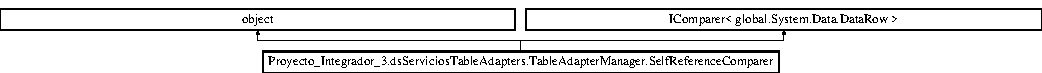
\includegraphics[height=0.975610cm]{class_proyecto___integrador__3_1_1ds_servicios_table_adapters_1_1_table_adapter_manager_1_1_self_reference_comparer}
\end{center}
\end{figure}
\subsection*{Métodos públicos}
\begin{DoxyCompactItemize}
\item 
int \hyperlink{class_proyecto___integrador__3_1_1ds_servicios_table_adapters_1_1_table_adapter_manager_1_1_self_reference_comparer_a8e226852fba6e592bf7d9a81be340051}{Compare} (global\-::\-System.\-Data.\-Data\-Row row1, global\-::\-System.\-Data.\-Data\-Row row2)
\end{DoxyCompactItemize}
\subsection*{Funciones del 'package'}
\begin{DoxyCompactItemize}
\item 
\hyperlink{class_proyecto___integrador__3_1_1ds_servicios_table_adapters_1_1_table_adapter_manager_1_1_self_reference_comparer_ab3a62ea6472e37e6d85704cdea28e806}{Self\-Reference\-Comparer} (global\-::\-System.\-Data.\-Data\-Relation relation, bool child\-First)
\end{DoxyCompactItemize}
\subsection*{Métodos privados}
\begin{DoxyCompactItemize}
\item 
global\-::\-System.\-Data.\-Data\-Row \hyperlink{class_proyecto___integrador__3_1_1ds_servicios_table_adapters_1_1_table_adapter_manager_1_1_self_reference_comparer_a9bf53ee3bb97ad3fc23f5d885290e9b4}{Get\-Root} (global\-::\-System.\-Data.\-Data\-Row row, out int distance)
\end{DoxyCompactItemize}
\subsection*{Atributos privados}
\begin{DoxyCompactItemize}
\item 
global\-::\-System.\-Data.\-Data\-Relation \hyperlink{class_proyecto___integrador__3_1_1ds_servicios_table_adapters_1_1_table_adapter_manager_1_1_self_reference_comparer_a88115b67b87d4305d472d5fa124304b0}{\-\_\-relation}
\item 
int \hyperlink{class_proyecto___integrador__3_1_1ds_servicios_table_adapters_1_1_table_adapter_manager_1_1_self_reference_comparer_abf5fed6c245e5ee78cd5472bac96e77e}{\-\_\-child\-First}
\end{DoxyCompactItemize}


\subsection{Descripción detallada}
Used to sort self-\/referenced table's rows /summary$>$ 

Definición en la línea 1347 del archivo ds\-Servicios.\-Designer.\-cs.



\subsection{Documentación del constructor y destructor}
\hypertarget{class_proyecto___integrador__3_1_1ds_servicios_table_adapters_1_1_table_adapter_manager_1_1_self_reference_comparer_ab3a62ea6472e37e6d85704cdea28e806}{\index{Proyecto\-\_\-\-Integrador\-\_\-3\-::ds\-Servicios\-Table\-Adapters\-::\-Table\-Adapter\-Manager\-::\-Self\-Reference\-Comparer@{Proyecto\-\_\-\-Integrador\-\_\-3\-::ds\-Servicios\-Table\-Adapters\-::\-Table\-Adapter\-Manager\-::\-Self\-Reference\-Comparer}!Self\-Reference\-Comparer@{Self\-Reference\-Comparer}}
\index{Self\-Reference\-Comparer@{Self\-Reference\-Comparer}!Proyecto_Integrador_3::dsServiciosTableAdapters::TableAdapterManager::SelfReferenceComparer@{Proyecto\-\_\-\-Integrador\-\_\-3\-::ds\-Servicios\-Table\-Adapters\-::\-Table\-Adapter\-Manager\-::\-Self\-Reference\-Comparer}}
\subsubsection[{Self\-Reference\-Comparer}]{\setlength{\rightskip}{0pt plus 5cm}Proyecto\-\_\-\-Integrador\-\_\-3.\-ds\-Servicios\-Table\-Adapters.\-Table\-Adapter\-Manager.\-Self\-Reference\-Comparer.\-Self\-Reference\-Comparer (
\begin{DoxyParamCaption}
\item[{global\-::\-System.\-Data.\-Data\-Relation}]{relation, }
\item[{bool}]{child\-First}
\end{DoxyParamCaption}
)\hspace{0.3cm}{\ttfamily [inline]}, {\ttfamily [package]}}}\label{class_proyecto___integrador__3_1_1ds_servicios_table_adapters_1_1_table_adapter_manager_1_1_self_reference_comparer_ab3a62ea6472e37e6d85704cdea28e806}


Definición en la línea 1355 del archivo ds\-Servicios.\-Designer.\-cs.


\begin{DoxyCode}
1355                                                                                                      \{
1356                 this.\hyperlink{class_proyecto___integrador__3_1_1ds_servicios_table_adapters_1_1_table_adapter_manager_1_1_self_reference_comparer_a88115b67b87d4305d472d5fa124304b0}{\_relation} = relation;
1357                 \textcolor{keywordflow}{if} (childFirst) \{
1358                     this.\hyperlink{class_proyecto___integrador__3_1_1ds_servicios_table_adapters_1_1_table_adapter_manager_1_1_self_reference_comparer_abf5fed6c245e5ee78cd5472bac96e77e}{\_childFirst} = -1;
1359                 \}
1360                 \textcolor{keywordflow}{else} \{
1361                     this.\hyperlink{class_proyecto___integrador__3_1_1ds_servicios_table_adapters_1_1_table_adapter_manager_1_1_self_reference_comparer_abf5fed6c245e5ee78cd5472bac96e77e}{\_childFirst} = 1;
1362                 \}
1363             \}
\end{DoxyCode}


\subsection{Documentación de las funciones miembro}
\hypertarget{class_proyecto___integrador__3_1_1ds_servicios_table_adapters_1_1_table_adapter_manager_1_1_self_reference_comparer_a8e226852fba6e592bf7d9a81be340051}{\index{Proyecto\-\_\-\-Integrador\-\_\-3\-::ds\-Servicios\-Table\-Adapters\-::\-Table\-Adapter\-Manager\-::\-Self\-Reference\-Comparer@{Proyecto\-\_\-\-Integrador\-\_\-3\-::ds\-Servicios\-Table\-Adapters\-::\-Table\-Adapter\-Manager\-::\-Self\-Reference\-Comparer}!Compare@{Compare}}
\index{Compare@{Compare}!Proyecto_Integrador_3::dsServiciosTableAdapters::TableAdapterManager::SelfReferenceComparer@{Proyecto\-\_\-\-Integrador\-\_\-3\-::ds\-Servicios\-Table\-Adapters\-::\-Table\-Adapter\-Manager\-::\-Self\-Reference\-Comparer}}
\subsubsection[{Compare}]{\setlength{\rightskip}{0pt plus 5cm}int Proyecto\-\_\-\-Integrador\-\_\-3.\-ds\-Servicios\-Table\-Adapters.\-Table\-Adapter\-Manager.\-Self\-Reference\-Comparer.\-Compare (
\begin{DoxyParamCaption}
\item[{global\-::\-System.\-Data.\-Data\-Row}]{row1, }
\item[{global\-::\-System.\-Data.\-Data\-Row}]{row2}
\end{DoxyParamCaption}
)\hspace{0.3cm}{\ttfamily [inline]}}}\label{class_proyecto___integrador__3_1_1ds_servicios_table_adapters_1_1_table_adapter_manager_1_1_self_reference_comparer_a8e226852fba6e592bf7d9a81be340051}


Definición en la línea 1406 del archivo ds\-Servicios.\-Designer.\-cs.


\begin{DoxyCode}
1406                                                                                                \{
1407                 \textcolor{keywordflow}{if} (\textcolor{keywordtype}{object}.ReferenceEquals(row1, row2)) \{
1408                     \textcolor{keywordflow}{return} 0;
1409                 \}
1410                 \textcolor{keywordflow}{if} ((row1 == null)) \{
1411                     \textcolor{keywordflow}{return} -1;
1412                 \}
1413                 \textcolor{keywordflow}{if} ((row2 == null)) \{
1414                     \textcolor{keywordflow}{return} 1;
1415                 \}
1416 
1417                 \textcolor{keywordtype}{int} distance1 = 0;
1418                 global::System.Data.DataRow root1 = this.\hyperlink{class_proyecto___integrador__3_1_1ds_servicios_table_adapters_1_1_table_adapter_manager_1_1_self_reference_comparer_a9bf53ee3bb97ad3fc23f5d885290e9b4}{GetRoot}(row1, out distance1);
1419 
1420                 \textcolor{keywordtype}{int} distance2 = 0;
1421                 global::System.Data.DataRow root2 = this.\hyperlink{class_proyecto___integrador__3_1_1ds_servicios_table_adapters_1_1_table_adapter_manager_1_1_self_reference_comparer_a9bf53ee3bb97ad3fc23f5d885290e9b4}{GetRoot}(row2, out distance2);
1422 
1423                 \textcolor{keywordflow}{if} (\textcolor{keywordtype}{object}.ReferenceEquals(root1, root2)) \{
1424                     \textcolor{keywordflow}{return} (this.\hyperlink{class_proyecto___integrador__3_1_1ds_servicios_table_adapters_1_1_table_adapter_manager_1_1_self_reference_comparer_abf5fed6c245e5ee78cd5472bac96e77e}{\_childFirst} * distance1.CompareTo(distance2));
1425                 \}
1426                 \textcolor{keywordflow}{else} \{
1427                     global::System.Diagnostics.Debug.Assert(((root1.Table != null) 
1428                                     && (root2.Table != null)));
1429                     \textcolor{keywordflow}{if} ((root1.Table.Rows.IndexOf(root1) < root2.Table.Rows.IndexOf(root2))) \{
1430                         \textcolor{keywordflow}{return} -1;
1431                     \}
1432                     \textcolor{keywordflow}{else} \{
1433                         \textcolor{keywordflow}{return} 1;
1434                     \}
1435                 \}
1436             \}
\end{DoxyCode}
\hypertarget{class_proyecto___integrador__3_1_1ds_servicios_table_adapters_1_1_table_adapter_manager_1_1_self_reference_comparer_a9bf53ee3bb97ad3fc23f5d885290e9b4}{\index{Proyecto\-\_\-\-Integrador\-\_\-3\-::ds\-Servicios\-Table\-Adapters\-::\-Table\-Adapter\-Manager\-::\-Self\-Reference\-Comparer@{Proyecto\-\_\-\-Integrador\-\_\-3\-::ds\-Servicios\-Table\-Adapters\-::\-Table\-Adapter\-Manager\-::\-Self\-Reference\-Comparer}!Get\-Root@{Get\-Root}}
\index{Get\-Root@{Get\-Root}!Proyecto_Integrador_3::dsServiciosTableAdapters::TableAdapterManager::SelfReferenceComparer@{Proyecto\-\_\-\-Integrador\-\_\-3\-::ds\-Servicios\-Table\-Adapters\-::\-Table\-Adapter\-Manager\-::\-Self\-Reference\-Comparer}}
\subsubsection[{Get\-Root}]{\setlength{\rightskip}{0pt plus 5cm}global.\-System.\-Data.\-Data\-Row Proyecto\-\_\-\-Integrador\-\_\-3.\-ds\-Servicios\-Table\-Adapters.\-Table\-Adapter\-Manager.\-Self\-Reference\-Comparer.\-Get\-Root (
\begin{DoxyParamCaption}
\item[{global\-::\-System.\-Data.\-Data\-Row}]{row, }
\item[{out int}]{distance}
\end{DoxyParamCaption}
)\hspace{0.3cm}{\ttfamily [inline]}, {\ttfamily [private]}}}\label{class_proyecto___integrador__3_1_1ds_servicios_table_adapters_1_1_table_adapter_manager_1_1_self_reference_comparer_a9bf53ee3bb97ad3fc23f5d885290e9b4}


Definición en la línea 1367 del archivo ds\-Servicios.\-Designer.\-cs.


\begin{DoxyCode}
1367                                                                                                        \{
1368                 global::System.Diagnostics.Debug.Assert((row != null));
1369                 global::System.Data.DataRow root = row;
1370                 distance = 0;
1371 
1372                 global::System.Collections.Generic.IDictionary<global::System.Data.DataRow, global::System.
      Data.DataRow> traversedRows = \textcolor{keyword}{new} global::System.Collections.Generic.Dictionary<global::System.Data.DataRow,
       global::System.Data.DataRow>();
1373                 traversedRows[row] = row;
1374 
1375                 global::System.Data.DataRow parent = row.GetParentRow(this.
      \hyperlink{class_proyecto___integrador__3_1_1ds_servicios_table_adapters_1_1_table_adapter_manager_1_1_self_reference_comparer_a88115b67b87d4305d472d5fa124304b0}{\_relation}, global::System.Data.DataRowVersion.Default);
1376                 \textcolor{keywordflow}{for} (
1377                 ; ((parent != null) 
1378                             && (traversedRows.ContainsKey(parent) == \textcolor{keyword}{false})); 
1379                 ) \{
1380                     distance = (distance + 1);
1381                     root = parent;
1382                     traversedRows[parent] = parent;
1383                     parent = parent.GetParentRow(this.\hyperlink{class_proyecto___integrador__3_1_1ds_servicios_table_adapters_1_1_table_adapter_manager_1_1_self_reference_comparer_a88115b67b87d4305d472d5fa124304b0}{\_relation}, global::System.Data.
      DataRowVersion.Default);
1384                 \}
1385 
1386                 \textcolor{keywordflow}{if} ((distance == 0)) \{
1387                     traversedRows.Clear();
1388                     traversedRows[row] = row;
1389                     parent = row.GetParentRow(this.\hyperlink{class_proyecto___integrador__3_1_1ds_servicios_table_adapters_1_1_table_adapter_manager_1_1_self_reference_comparer_a88115b67b87d4305d472d5fa124304b0}{\_relation}, global::System.Data.DataRowVersion.
      Original);
1390                     \textcolor{keywordflow}{for} (
1391                     ; ((parent != null) 
1392                                 && (traversedRows.ContainsKey(parent) == \textcolor{keyword}{false})); 
1393                     ) \{
1394                         distance = (distance + 1);
1395                         root = parent;
1396                         traversedRows[parent] = parent;
1397                         parent = parent.GetParentRow(this.\hyperlink{class_proyecto___integrador__3_1_1ds_servicios_table_adapters_1_1_table_adapter_manager_1_1_self_reference_comparer_a88115b67b87d4305d472d5fa124304b0}{\_relation}, global::System.Data.
      DataRowVersion.Original);
1398                     \}
1399                 \}
1400 
1401                 \textcolor{keywordflow}{return} root;
1402             \}
\end{DoxyCode}


\subsection{Documentación de los datos miembro}
\hypertarget{class_proyecto___integrador__3_1_1ds_servicios_table_adapters_1_1_table_adapter_manager_1_1_self_reference_comparer_abf5fed6c245e5ee78cd5472bac96e77e}{\index{Proyecto\-\_\-\-Integrador\-\_\-3\-::ds\-Servicios\-Table\-Adapters\-::\-Table\-Adapter\-Manager\-::\-Self\-Reference\-Comparer@{Proyecto\-\_\-\-Integrador\-\_\-3\-::ds\-Servicios\-Table\-Adapters\-::\-Table\-Adapter\-Manager\-::\-Self\-Reference\-Comparer}!\-\_\-child\-First@{\-\_\-child\-First}}
\index{\-\_\-child\-First@{\-\_\-child\-First}!Proyecto_Integrador_3::dsServiciosTableAdapters::TableAdapterManager::SelfReferenceComparer@{Proyecto\-\_\-\-Integrador\-\_\-3\-::ds\-Servicios\-Table\-Adapters\-::\-Table\-Adapter\-Manager\-::\-Self\-Reference\-Comparer}}
\subsubsection[{\-\_\-child\-First}]{\setlength{\rightskip}{0pt plus 5cm}int Proyecto\-\_\-\-Integrador\-\_\-3.\-ds\-Servicios\-Table\-Adapters.\-Table\-Adapter\-Manager.\-Self\-Reference\-Comparer.\-\_\-child\-First\hspace{0.3cm}{\ttfamily [private]}}}\label{class_proyecto___integrador__3_1_1ds_servicios_table_adapters_1_1_table_adapter_manager_1_1_self_reference_comparer_abf5fed6c245e5ee78cd5472bac96e77e}


Definición en la línea 1351 del archivo ds\-Servicios.\-Designer.\-cs.

\hypertarget{class_proyecto___integrador__3_1_1ds_servicios_table_adapters_1_1_table_adapter_manager_1_1_self_reference_comparer_a88115b67b87d4305d472d5fa124304b0}{\index{Proyecto\-\_\-\-Integrador\-\_\-3\-::ds\-Servicios\-Table\-Adapters\-::\-Table\-Adapter\-Manager\-::\-Self\-Reference\-Comparer@{Proyecto\-\_\-\-Integrador\-\_\-3\-::ds\-Servicios\-Table\-Adapters\-::\-Table\-Adapter\-Manager\-::\-Self\-Reference\-Comparer}!\-\_\-relation@{\-\_\-relation}}
\index{\-\_\-relation@{\-\_\-relation}!Proyecto_Integrador_3::dsServiciosTableAdapters::TableAdapterManager::SelfReferenceComparer@{Proyecto\-\_\-\-Integrador\-\_\-3\-::ds\-Servicios\-Table\-Adapters\-::\-Table\-Adapter\-Manager\-::\-Self\-Reference\-Comparer}}
\subsubsection[{\-\_\-relation}]{\setlength{\rightskip}{0pt plus 5cm}global.\-System.\-Data.\-Data\-Relation Proyecto\-\_\-\-Integrador\-\_\-3.\-ds\-Servicios\-Table\-Adapters.\-Table\-Adapter\-Manager.\-Self\-Reference\-Comparer.\-\_\-relation\hspace{0.3cm}{\ttfamily [private]}}}\label{class_proyecto___integrador__3_1_1ds_servicios_table_adapters_1_1_table_adapter_manager_1_1_self_reference_comparer_a88115b67b87d4305d472d5fa124304b0}


Definición en la línea 1349 del archivo ds\-Servicios.\-Designer.\-cs.



La documentación para esta clase fue generada a partir del siguiente fichero\-:\begin{DoxyCompactItemize}
\item 
C\-:/\-Users/\-Yknx4/\-Documents/\-Visual Studio 2012/\-Projects/\-Proyecto Integrador 3/\-Proyecto Integrador 3/\hyperlink{ds_servicios_8_designer_8cs}{ds\-Servicios.\-Designer.\-cs}\end{DoxyCompactItemize}

\hypertarget{class_proyecto___integrador__3_1_1ds_usuarios_table_adapters_1_1_table_adapter_manager_1_1_self_reference_comparer}{\section{Referencia de la Clase Proyecto\-\_\-\-Integrador\-\_\-3.\-ds\-Usuarios\-Table\-Adapters.\-Table\-Adapter\-Manager.\-Self\-Reference\-Comparer}
\label{class_proyecto___integrador__3_1_1ds_usuarios_table_adapters_1_1_table_adapter_manager_1_1_self_reference_comparer}\index{Proyecto\-\_\-\-Integrador\-\_\-3.\-ds\-Usuarios\-Table\-Adapters.\-Table\-Adapter\-Manager.\-Self\-Reference\-Comparer@{Proyecto\-\_\-\-Integrador\-\_\-3.\-ds\-Usuarios\-Table\-Adapters.\-Table\-Adapter\-Manager.\-Self\-Reference\-Comparer}}
}


Used to sort self-\/referenced table's rows /summary$>$  


Diagrama de herencias de Proyecto\-\_\-\-Integrador\-\_\-3.\-ds\-Usuarios\-Table\-Adapters.\-Table\-Adapter\-Manager.\-Self\-Reference\-Comparer\begin{figure}[H]
\begin{center}
\leavevmode
\includegraphics[height=0.982456cm]{d9/dfc/class_proyecto___integrador__3_1_1ds_usuarios_table_adapters_1_1_table_adapter_manager_1_1_self_reference_comparer}
\end{center}
\end{figure}
\subsection*{Métodos públicos}
\begin{DoxyCompactItemize}
\item 
int \hyperlink{class_proyecto___integrador__3_1_1ds_usuarios_table_adapters_1_1_table_adapter_manager_1_1_self_reference_comparer_a78c217a295562cf7990f8af9d8dd393c}{Compare} (global\-::\-System.\-Data.\-Data\-Row row1, global\-::\-System.\-Data.\-Data\-Row row2)
\end{DoxyCompactItemize}
\subsection*{Funciones del 'package'}
\begin{DoxyCompactItemize}
\item 
\hyperlink{class_proyecto___integrador__3_1_1ds_usuarios_table_adapters_1_1_table_adapter_manager_1_1_self_reference_comparer_a48369f8c120506a95bdb9be253dddd7d}{Self\-Reference\-Comparer} (global\-::\-System.\-Data.\-Data\-Relation relation, bool child\-First)
\end{DoxyCompactItemize}
\subsection*{Métodos privados}
\begin{DoxyCompactItemize}
\item 
global\-::\-System.\-Data.\-Data\-Row \hyperlink{class_proyecto___integrador__3_1_1ds_usuarios_table_adapters_1_1_table_adapter_manager_1_1_self_reference_comparer_adbe612a7a1ed56040974c39de179a041}{Get\-Root} (global\-::\-System.\-Data.\-Data\-Row row, out int distance)
\end{DoxyCompactItemize}
\subsection*{Atributos privados}
\begin{DoxyCompactItemize}
\item 
global\-::\-System.\-Data.\-Data\-Relation \hyperlink{class_proyecto___integrador__3_1_1ds_usuarios_table_adapters_1_1_table_adapter_manager_1_1_self_reference_comparer_aa94b2ca3f3ea52c71719c2b968ae574a}{\-\_\-relation}
\item 
int \hyperlink{class_proyecto___integrador__3_1_1ds_usuarios_table_adapters_1_1_table_adapter_manager_1_1_self_reference_comparer_a0d9b911f3c6ab73098107a9d88aa85c6}{\-\_\-child\-First}
\end{DoxyCompactItemize}


\subsection{Descripción detallada}
Used to sort self-\/referenced table's rows /summary$>$ 

Definición en la línea 2210 del archivo ds\-Usuarios.\-Designer.\-cs.



\subsection{Documentación del constructor y destructor}
\hypertarget{class_proyecto___integrador__3_1_1ds_usuarios_table_adapters_1_1_table_adapter_manager_1_1_self_reference_comparer_a48369f8c120506a95bdb9be253dddd7d}{\index{Proyecto\-\_\-\-Integrador\-\_\-3\-::ds\-Usuarios\-Table\-Adapters\-::\-Table\-Adapter\-Manager\-::\-Self\-Reference\-Comparer@{Proyecto\-\_\-\-Integrador\-\_\-3\-::ds\-Usuarios\-Table\-Adapters\-::\-Table\-Adapter\-Manager\-::\-Self\-Reference\-Comparer}!Self\-Reference\-Comparer@{Self\-Reference\-Comparer}}
\index{Self\-Reference\-Comparer@{Self\-Reference\-Comparer}!Proyecto_Integrador_3::dsUsuariosTableAdapters::TableAdapterManager::SelfReferenceComparer@{Proyecto\-\_\-\-Integrador\-\_\-3\-::ds\-Usuarios\-Table\-Adapters\-::\-Table\-Adapter\-Manager\-::\-Self\-Reference\-Comparer}}
\subsubsection[{Self\-Reference\-Comparer}]{\setlength{\rightskip}{0pt plus 5cm}Proyecto\-\_\-\-Integrador\-\_\-3.\-ds\-Usuarios\-Table\-Adapters.\-Table\-Adapter\-Manager.\-Self\-Reference\-Comparer.\-Self\-Reference\-Comparer (
\begin{DoxyParamCaption}
\item[{global\-::\-System.\-Data.\-Data\-Relation}]{relation, }
\item[{bool}]{child\-First}
\end{DoxyParamCaption}
)\hspace{0.3cm}{\ttfamily [inline]}, {\ttfamily [package]}}}\label{class_proyecto___integrador__3_1_1ds_usuarios_table_adapters_1_1_table_adapter_manager_1_1_self_reference_comparer_a48369f8c120506a95bdb9be253dddd7d}


Definición en la línea 2218 del archivo ds\-Usuarios.\-Designer.\-cs.


\begin{DoxyCode}
2218                                                                                                      \{
2219                 this.\hyperlink{class_proyecto___integrador__3_1_1ds_usuarios_table_adapters_1_1_table_adapter_manager_1_1_self_reference_comparer_aa94b2ca3f3ea52c71719c2b968ae574a}{\_relation} = relation;
2220                 \textcolor{keywordflow}{if} (childFirst) \{
2221                     this.\hyperlink{class_proyecto___integrador__3_1_1ds_usuarios_table_adapters_1_1_table_adapter_manager_1_1_self_reference_comparer_a0d9b911f3c6ab73098107a9d88aa85c6}{\_childFirst} = -1;
2222                 \}
2223                 \textcolor{keywordflow}{else} \{
2224                     this.\hyperlink{class_proyecto___integrador__3_1_1ds_usuarios_table_adapters_1_1_table_adapter_manager_1_1_self_reference_comparer_a0d9b911f3c6ab73098107a9d88aa85c6}{\_childFirst} = 1;
2225                 \}
2226             \}
\end{DoxyCode}


\subsection{Documentación de las funciones miembro}
\hypertarget{class_proyecto___integrador__3_1_1ds_usuarios_table_adapters_1_1_table_adapter_manager_1_1_self_reference_comparer_a78c217a295562cf7990f8af9d8dd393c}{\index{Proyecto\-\_\-\-Integrador\-\_\-3\-::ds\-Usuarios\-Table\-Adapters\-::\-Table\-Adapter\-Manager\-::\-Self\-Reference\-Comparer@{Proyecto\-\_\-\-Integrador\-\_\-3\-::ds\-Usuarios\-Table\-Adapters\-::\-Table\-Adapter\-Manager\-::\-Self\-Reference\-Comparer}!Compare@{Compare}}
\index{Compare@{Compare}!Proyecto_Integrador_3::dsUsuariosTableAdapters::TableAdapterManager::SelfReferenceComparer@{Proyecto\-\_\-\-Integrador\-\_\-3\-::ds\-Usuarios\-Table\-Adapters\-::\-Table\-Adapter\-Manager\-::\-Self\-Reference\-Comparer}}
\subsubsection[{Compare}]{\setlength{\rightskip}{0pt plus 5cm}int Proyecto\-\_\-\-Integrador\-\_\-3.\-ds\-Usuarios\-Table\-Adapters.\-Table\-Adapter\-Manager.\-Self\-Reference\-Comparer.\-Compare (
\begin{DoxyParamCaption}
\item[{global\-::\-System.\-Data.\-Data\-Row}]{row1, }
\item[{global\-::\-System.\-Data.\-Data\-Row}]{row2}
\end{DoxyParamCaption}
)\hspace{0.3cm}{\ttfamily [inline]}}}\label{class_proyecto___integrador__3_1_1ds_usuarios_table_adapters_1_1_table_adapter_manager_1_1_self_reference_comparer_a78c217a295562cf7990f8af9d8dd393c}


Definición en la línea 2269 del archivo ds\-Usuarios.\-Designer.\-cs.


\begin{DoxyCode}
2269                                                                                                \{
2270                 \textcolor{keywordflow}{if} (\textcolor{keywordtype}{object}.ReferenceEquals(row1, row2)) \{
2271                     \textcolor{keywordflow}{return} 0;
2272                 \}
2273                 \textcolor{keywordflow}{if} ((row1 == null)) \{
2274                     \textcolor{keywordflow}{return} -1;
2275                 \}
2276                 \textcolor{keywordflow}{if} ((row2 == null)) \{
2277                     \textcolor{keywordflow}{return} 1;
2278                 \}
2279 
2280                 \textcolor{keywordtype}{int} distance1 = 0;
2281                 global::System.Data.DataRow root1 = this.\hyperlink{class_proyecto___integrador__3_1_1ds_usuarios_table_adapters_1_1_table_adapter_manager_1_1_self_reference_comparer_adbe612a7a1ed56040974c39de179a041}{GetRoot}(row1, out distance1);
2282 
2283                 \textcolor{keywordtype}{int} distance2 = 0;
2284                 global::System.Data.DataRow root2 = this.\hyperlink{class_proyecto___integrador__3_1_1ds_usuarios_table_adapters_1_1_table_adapter_manager_1_1_self_reference_comparer_adbe612a7a1ed56040974c39de179a041}{GetRoot}(row2, out distance2);
2285 
2286                 \textcolor{keywordflow}{if} (\textcolor{keywordtype}{object}.ReferenceEquals(root1, root2)) \{
2287                     \textcolor{keywordflow}{return} (this.\hyperlink{class_proyecto___integrador__3_1_1ds_usuarios_table_adapters_1_1_table_adapter_manager_1_1_self_reference_comparer_a0d9b911f3c6ab73098107a9d88aa85c6}{\_childFirst} * distance1.CompareTo(distance2));
2288                 \}
2289                 \textcolor{keywordflow}{else} \{
2290                     global::System.Diagnostics.Debug.Assert(((root1.Table != null) 
2291                                     && (root2.Table != null)));
2292                     \textcolor{keywordflow}{if} ((root1.Table.Rows.IndexOf(root1) < root2.Table.Rows.IndexOf(root2))) \{
2293                         \textcolor{keywordflow}{return} -1;
2294                     \}
2295                     \textcolor{keywordflow}{else} \{
2296                         \textcolor{keywordflow}{return} 1;
2297                     \}
2298                 \}
2299             \}
\end{DoxyCode}
\hypertarget{class_proyecto___integrador__3_1_1ds_usuarios_table_adapters_1_1_table_adapter_manager_1_1_self_reference_comparer_adbe612a7a1ed56040974c39de179a041}{\index{Proyecto\-\_\-\-Integrador\-\_\-3\-::ds\-Usuarios\-Table\-Adapters\-::\-Table\-Adapter\-Manager\-::\-Self\-Reference\-Comparer@{Proyecto\-\_\-\-Integrador\-\_\-3\-::ds\-Usuarios\-Table\-Adapters\-::\-Table\-Adapter\-Manager\-::\-Self\-Reference\-Comparer}!Get\-Root@{Get\-Root}}
\index{Get\-Root@{Get\-Root}!Proyecto_Integrador_3::dsUsuariosTableAdapters::TableAdapterManager::SelfReferenceComparer@{Proyecto\-\_\-\-Integrador\-\_\-3\-::ds\-Usuarios\-Table\-Adapters\-::\-Table\-Adapter\-Manager\-::\-Self\-Reference\-Comparer}}
\subsubsection[{Get\-Root}]{\setlength{\rightskip}{0pt plus 5cm}global.\-System.\-Data.\-Data\-Row Proyecto\-\_\-\-Integrador\-\_\-3.\-ds\-Usuarios\-Table\-Adapters.\-Table\-Adapter\-Manager.\-Self\-Reference\-Comparer.\-Get\-Root (
\begin{DoxyParamCaption}
\item[{global\-::\-System.\-Data.\-Data\-Row}]{row, }
\item[{out int}]{distance}
\end{DoxyParamCaption}
)\hspace{0.3cm}{\ttfamily [inline]}, {\ttfamily [private]}}}\label{class_proyecto___integrador__3_1_1ds_usuarios_table_adapters_1_1_table_adapter_manager_1_1_self_reference_comparer_adbe612a7a1ed56040974c39de179a041}


Definición en la línea 2230 del archivo ds\-Usuarios.\-Designer.\-cs.


\begin{DoxyCode}
2230                                                                                                        \{
2231                 global::System.Diagnostics.Debug.Assert((row != null));
2232                 global::System.Data.DataRow root = row;
2233                 distance = 0;
2234 
2235                 global::System.Collections.Generic.IDictionary<global::System.Data.DataRow, global::System.
      Data.DataRow> traversedRows = \textcolor{keyword}{new} global::System.Collections.Generic.Dictionary<global::System.Data.DataRow,
       global::System.Data.DataRow>();
2236                 traversedRows[row] = row;
2237 
2238                 global::System.Data.DataRow parent = row.GetParentRow(this.
      \hyperlink{class_proyecto___integrador__3_1_1ds_usuarios_table_adapters_1_1_table_adapter_manager_1_1_self_reference_comparer_aa94b2ca3f3ea52c71719c2b968ae574a}{\_relation}, global::System.Data.DataRowVersion.Default);
2239                 \textcolor{keywordflow}{for} (
2240                 ; ((parent != null) 
2241                             && (traversedRows.ContainsKey(parent) == \textcolor{keyword}{false})); 
2242                 ) \{
2243                     distance = (distance + 1);
2244                     root = parent;
2245                     traversedRows[parent] = parent;
2246                     parent = parent.GetParentRow(this.\hyperlink{class_proyecto___integrador__3_1_1ds_usuarios_table_adapters_1_1_table_adapter_manager_1_1_self_reference_comparer_aa94b2ca3f3ea52c71719c2b968ae574a}{\_relation}, global::System.Data.
      DataRowVersion.Default);
2247                 \}
2248 
2249                 \textcolor{keywordflow}{if} ((distance == 0)) \{
2250                     traversedRows.Clear();
2251                     traversedRows[row] = row;
2252                     parent = row.GetParentRow(this.\hyperlink{class_proyecto___integrador__3_1_1ds_usuarios_table_adapters_1_1_table_adapter_manager_1_1_self_reference_comparer_aa94b2ca3f3ea52c71719c2b968ae574a}{\_relation}, global::System.Data.DataRowVersion.
      Original);
2253                     \textcolor{keywordflow}{for} (
2254                     ; ((parent != null) 
2255                                 && (traversedRows.ContainsKey(parent) == \textcolor{keyword}{false})); 
2256                     ) \{
2257                         distance = (distance + 1);
2258                         root = parent;
2259                         traversedRows[parent] = parent;
2260                         parent = parent.GetParentRow(this.\hyperlink{class_proyecto___integrador__3_1_1ds_usuarios_table_adapters_1_1_table_adapter_manager_1_1_self_reference_comparer_aa94b2ca3f3ea52c71719c2b968ae574a}{\_relation}, global::System.Data.
      DataRowVersion.Original);
2261                     \}
2262                 \}
2263 
2264                 \textcolor{keywordflow}{return} root;
2265             \}
\end{DoxyCode}


\subsection{Documentación de los datos miembro}
\hypertarget{class_proyecto___integrador__3_1_1ds_usuarios_table_adapters_1_1_table_adapter_manager_1_1_self_reference_comparer_a0d9b911f3c6ab73098107a9d88aa85c6}{\index{Proyecto\-\_\-\-Integrador\-\_\-3\-::ds\-Usuarios\-Table\-Adapters\-::\-Table\-Adapter\-Manager\-::\-Self\-Reference\-Comparer@{Proyecto\-\_\-\-Integrador\-\_\-3\-::ds\-Usuarios\-Table\-Adapters\-::\-Table\-Adapter\-Manager\-::\-Self\-Reference\-Comparer}!\-\_\-child\-First@{\-\_\-child\-First}}
\index{\-\_\-child\-First@{\-\_\-child\-First}!Proyecto_Integrador_3::dsUsuariosTableAdapters::TableAdapterManager::SelfReferenceComparer@{Proyecto\-\_\-\-Integrador\-\_\-3\-::ds\-Usuarios\-Table\-Adapters\-::\-Table\-Adapter\-Manager\-::\-Self\-Reference\-Comparer}}
\subsubsection[{\-\_\-child\-First}]{\setlength{\rightskip}{0pt plus 5cm}int Proyecto\-\_\-\-Integrador\-\_\-3.\-ds\-Usuarios\-Table\-Adapters.\-Table\-Adapter\-Manager.\-Self\-Reference\-Comparer.\-\_\-child\-First\hspace{0.3cm}{\ttfamily [private]}}}\label{class_proyecto___integrador__3_1_1ds_usuarios_table_adapters_1_1_table_adapter_manager_1_1_self_reference_comparer_a0d9b911f3c6ab73098107a9d88aa85c6}


Definición en la línea 2214 del archivo ds\-Usuarios.\-Designer.\-cs.

\hypertarget{class_proyecto___integrador__3_1_1ds_usuarios_table_adapters_1_1_table_adapter_manager_1_1_self_reference_comparer_aa94b2ca3f3ea52c71719c2b968ae574a}{\index{Proyecto\-\_\-\-Integrador\-\_\-3\-::ds\-Usuarios\-Table\-Adapters\-::\-Table\-Adapter\-Manager\-::\-Self\-Reference\-Comparer@{Proyecto\-\_\-\-Integrador\-\_\-3\-::ds\-Usuarios\-Table\-Adapters\-::\-Table\-Adapter\-Manager\-::\-Self\-Reference\-Comparer}!\-\_\-relation@{\-\_\-relation}}
\index{\-\_\-relation@{\-\_\-relation}!Proyecto_Integrador_3::dsUsuariosTableAdapters::TableAdapterManager::SelfReferenceComparer@{Proyecto\-\_\-\-Integrador\-\_\-3\-::ds\-Usuarios\-Table\-Adapters\-::\-Table\-Adapter\-Manager\-::\-Self\-Reference\-Comparer}}
\subsubsection[{\-\_\-relation}]{\setlength{\rightskip}{0pt plus 5cm}global.\-System.\-Data.\-Data\-Relation Proyecto\-\_\-\-Integrador\-\_\-3.\-ds\-Usuarios\-Table\-Adapters.\-Table\-Adapter\-Manager.\-Self\-Reference\-Comparer.\-\_\-relation\hspace{0.3cm}{\ttfamily [private]}}}\label{class_proyecto___integrador__3_1_1ds_usuarios_table_adapters_1_1_table_adapter_manager_1_1_self_reference_comparer_aa94b2ca3f3ea52c71719c2b968ae574a}


Definición en la línea 2212 del archivo ds\-Usuarios.\-Designer.\-cs.



La documentación para esta clase fue generada a partir del siguiente fichero\-:\begin{DoxyCompactItemize}
\item 
C\-:/\-Users/\-Yknx4/\-Documents/\-Visual Studio 2012/\-Projects/\-Proyecto Integrador 3/\-Proyecto Integrador 3/\hyperlink{ds_usuarios_8_designer_8cs}{ds\-Usuarios.\-Designer.\-cs}\end{DoxyCompactItemize}

\hypertarget{class_proyecto___integrador__3_1_1_tipos_dato_1_1_servicio}{\section{Referencia de la Clase Proyecto\-\_\-\-Integrador\-\_\-3.\-Tipos\-Dato.\-Servicio}
\label{class_proyecto___integrador__3_1_1_tipos_dato_1_1_servicio}\index{Proyecto\-\_\-\-Integrador\-\_\-3.\-Tipos\-Dato.\-Servicio@{Proyecto\-\_\-\-Integrador\-\_\-3.\-Tipos\-Dato.\-Servicio}}
}
Diagrama de herencias de Proyecto\-\_\-\-Integrador\-\_\-3.\-Tipos\-Dato.\-Servicio\begin{figure}[H]
\begin{center}
\leavevmode
\includegraphics[height=2.000000cm]{da/de4/class_proyecto___integrador__3_1_1_tipos_dato_1_1_servicio}
\end{center}
\end{figure}
\subsection*{Métodos públicos}
\begin{DoxyCompactItemize}
\item 
override bool \hyperlink{class_proyecto___integrador__3_1_1_tipos_dato_1_1_servicio_a84ccd70aa17d65df0afff55a14faeeec}{is\-Added} ()
\begin{DoxyCompactList}\small\item\em Determina si esta instancia esta agregada a la base de datos. \end{DoxyCompactList}\end{DoxyCompactItemize}
\subsection*{Propiedades}
\begin{DoxyCompactItemize}
\item 
long \hyperlink{class_proyecto___integrador__3_1_1_tipos_dato_1_1_servicio_a81c451c62cc6b77b6f80614df5ffb80d}{Id}\hspace{0.3cm}{\ttfamily  \mbox{[}get, set\mbox{]}}
\item 
short \hyperlink{class_proyecto___integrador__3_1_1_tipos_dato_1_1_servicio_a756753eda712db3ba3d85b87bd35ba3a}{Tipo\-Usuario}\hspace{0.3cm}{\ttfamily  \mbox{[}get, set\mbox{]}}
\item 
System.\-Guid \hyperlink{class_proyecto___integrador__3_1_1_tipos_dato_1_1_servicio_a44520809b1552502c483547044c33d6e}{Unidad}\hspace{0.3cm}{\ttfamily  \mbox{[}get, set\mbox{]}}
\item 
System.\-Guid \hyperlink{class_proyecto___integrador__3_1_1_tipos_dato_1_1_servicio_a9321964b41ee188556767aabeecfc737}{Usuario}\hspace{0.3cm}{\ttfamily  \mbox{[}get, set\mbox{]}}
\item 
System.\-Date\-Time \hyperlink{class_proyecto___integrador__3_1_1_tipos_dato_1_1_servicio_adfd9654485b999c795437dee578fac98}{Fecha}\hspace{0.3cm}{\ttfamily  \mbox{[}get, set\mbox{]}}
\item 
virtual \hyperlink{class_proyecto___integrador__3_1_1_tipos_dato_1_1_unidad}{Unidad} \hyperlink{class_proyecto___integrador__3_1_1_tipos_dato_1_1_servicio_acc976af62324d86c48a8143ae605dc07}{Unidad\-Object}\hspace{0.3cm}{\ttfamily  \mbox{[}get, set\mbox{]}}
\item 
virtual string \hyperlink{class_proyecto___integrador__3_1_1_tipos_dato_1_1_servicio_abb92d5f6f972c2df3a7cbe4d25b713e8}{No\-Unidad}\hspace{0.3cm}{\ttfamily  \mbox{[}get, set\mbox{]}}
\item 
virtual \hyperlink{class_proyecto___integrador__3_1_1_tipos_dato_1_1_usuario}{Usuario} \hyperlink{class_proyecto___integrador__3_1_1_tipos_dato_1_1_servicio_addfdec1cd1f2629003b19752e0e0020b}{Usuario\-Object}\hspace{0.3cm}{\ttfamily  \mbox{[}get, set\mbox{]}}
\end{DoxyCompactItemize}
\subsection*{Atributos privados}
\begin{DoxyCompactItemize}
\item 
long \hyperlink{class_proyecto___integrador__3_1_1_tipos_dato_1_1_servicio_a127ad69f3c770d82a248b73276e41388}{\-\_\-id}
\item 
short \hyperlink{class_proyecto___integrador__3_1_1_tipos_dato_1_1_servicio_a2787eb24fd380da2cd0abe7b0e87ce2e}{\-\_\-tipo\-Usuario}
\item 
System.\-Guid \hyperlink{class_proyecto___integrador__3_1_1_tipos_dato_1_1_servicio_a4963d49bd3ca49ff2223c7a37469a23f}{\-\_\-unidad}
\item 
System.\-Guid \hyperlink{class_proyecto___integrador__3_1_1_tipos_dato_1_1_servicio_aea0939faf5d7273f1cb5a9cf7fd88896}{\-\_\-usuario}
\item 
Date\-Time \hyperlink{class_proyecto___integrador__3_1_1_tipos_dato_1_1_servicio_af33dd41383dbfde1410187bcb1951b95}{\-\_\-fecha}
\end{DoxyCompactItemize}


\subsection{Descripción detallada}


Definición en la línea 5 del archivo Servicio.\-cs.



\subsection{Documentación de las funciones miembro}
\hypertarget{class_proyecto___integrador__3_1_1_tipos_dato_1_1_servicio_a84ccd70aa17d65df0afff55a14faeeec}{\index{Proyecto\-\_\-\-Integrador\-\_\-3\-::\-Tipos\-Dato\-::\-Servicio@{Proyecto\-\_\-\-Integrador\-\_\-3\-::\-Tipos\-Dato\-::\-Servicio}!is\-Added@{is\-Added}}
\index{is\-Added@{is\-Added}!Proyecto_Integrador_3::TiposDato::Servicio@{Proyecto\-\_\-\-Integrador\-\_\-3\-::\-Tipos\-Dato\-::\-Servicio}}
\subsubsection[{is\-Added}]{\setlength{\rightskip}{0pt plus 5cm}override bool Proyecto\-\_\-\-Integrador\-\_\-3.\-Tipos\-Dato.\-Servicio.\-is\-Added (
\begin{DoxyParamCaption}
{}
\end{DoxyParamCaption}
)\hspace{0.3cm}{\ttfamily [virtual]}}}\label{class_proyecto___integrador__3_1_1_tipos_dato_1_1_servicio_a84ccd70aa17d65df0afff55a14faeeec}


Determina si esta instancia esta agregada a la base de datos. 

\begin{DoxyReturn}{Devuelve}
Verdadero si esta agregada, falso si no
\end{DoxyReturn}


Reimplementado de \hyperlink{class_proyecto___integrador__3_1_1_tipos_dato_1_1_d_b_item_ab88d7eef0fa58d7d5fdf40039867dd6e}{Proyecto\-\_\-\-Integrador\-\_\-3.\-Tipos\-Dato.\-D\-B\-Item}.



Definición en la línea 33 del archivo Servicio.\-cs.


\begin{DoxyCode}
34         \{
35             \textcolor{keywordflow}{return} !(\hyperlink{class_proyecto___integrador__3_1_1_tipos_dato_1_1_servicio_a81c451c62cc6b77b6f80614df5ffb80d}{Id} == 0);
36         \}
\end{DoxyCode}


\subsection{Documentación de los datos miembro}
\hypertarget{class_proyecto___integrador__3_1_1_tipos_dato_1_1_servicio_af33dd41383dbfde1410187bcb1951b95}{\index{Proyecto\-\_\-\-Integrador\-\_\-3\-::\-Tipos\-Dato\-::\-Servicio@{Proyecto\-\_\-\-Integrador\-\_\-3\-::\-Tipos\-Dato\-::\-Servicio}!\-\_\-fecha@{\-\_\-fecha}}
\index{\-\_\-fecha@{\-\_\-fecha}!Proyecto_Integrador_3::TiposDato::Servicio@{Proyecto\-\_\-\-Integrador\-\_\-3\-::\-Tipos\-Dato\-::\-Servicio}}
\subsubsection[{\-\_\-fecha}]{\setlength{\rightskip}{0pt plus 5cm}Date\-Time Proyecto\-\_\-\-Integrador\-\_\-3.\-Tipos\-Dato.\-Servicio.\-\_\-fecha\hspace{0.3cm}{\ttfamily [private]}}}\label{class_proyecto___integrador__3_1_1_tipos_dato_1_1_servicio_af33dd41383dbfde1410187bcb1951b95}


Definición en la línea 23 del archivo Servicio.\-cs.

\hypertarget{class_proyecto___integrador__3_1_1_tipos_dato_1_1_servicio_a127ad69f3c770d82a248b73276e41388}{\index{Proyecto\-\_\-\-Integrador\-\_\-3\-::\-Tipos\-Dato\-::\-Servicio@{Proyecto\-\_\-\-Integrador\-\_\-3\-::\-Tipos\-Dato\-::\-Servicio}!\-\_\-id@{\-\_\-id}}
\index{\-\_\-id@{\-\_\-id}!Proyecto_Integrador_3::TiposDato::Servicio@{Proyecto\-\_\-\-Integrador\-\_\-3\-::\-Tipos\-Dato\-::\-Servicio}}
\subsubsection[{\-\_\-id}]{\setlength{\rightskip}{0pt plus 5cm}long Proyecto\-\_\-\-Integrador\-\_\-3.\-Tipos\-Dato.\-Servicio.\-\_\-id\hspace{0.3cm}{\ttfamily [private]}}}\label{class_proyecto___integrador__3_1_1_tipos_dato_1_1_servicio_a127ad69f3c770d82a248b73276e41388}


Definición en la línea 7 del archivo Servicio.\-cs.

\hypertarget{class_proyecto___integrador__3_1_1_tipos_dato_1_1_servicio_a2787eb24fd380da2cd0abe7b0e87ce2e}{\index{Proyecto\-\_\-\-Integrador\-\_\-3\-::\-Tipos\-Dato\-::\-Servicio@{Proyecto\-\_\-\-Integrador\-\_\-3\-::\-Tipos\-Dato\-::\-Servicio}!\-\_\-tipo\-Usuario@{\-\_\-tipo\-Usuario}}
\index{\-\_\-tipo\-Usuario@{\-\_\-tipo\-Usuario}!Proyecto_Integrador_3::TiposDato::Servicio@{Proyecto\-\_\-\-Integrador\-\_\-3\-::\-Tipos\-Dato\-::\-Servicio}}
\subsubsection[{\-\_\-tipo\-Usuario}]{\setlength{\rightskip}{0pt plus 5cm}short Proyecto\-\_\-\-Integrador\-\_\-3.\-Tipos\-Dato.\-Servicio.\-\_\-tipo\-Usuario\hspace{0.3cm}{\ttfamily [private]}}}\label{class_proyecto___integrador__3_1_1_tipos_dato_1_1_servicio_a2787eb24fd380da2cd0abe7b0e87ce2e}


Definición en la línea 11 del archivo Servicio.\-cs.

\hypertarget{class_proyecto___integrador__3_1_1_tipos_dato_1_1_servicio_a4963d49bd3ca49ff2223c7a37469a23f}{\index{Proyecto\-\_\-\-Integrador\-\_\-3\-::\-Tipos\-Dato\-::\-Servicio@{Proyecto\-\_\-\-Integrador\-\_\-3\-::\-Tipos\-Dato\-::\-Servicio}!\-\_\-unidad@{\-\_\-unidad}}
\index{\-\_\-unidad@{\-\_\-unidad}!Proyecto_Integrador_3::TiposDato::Servicio@{Proyecto\-\_\-\-Integrador\-\_\-3\-::\-Tipos\-Dato\-::\-Servicio}}
\subsubsection[{\-\_\-unidad}]{\setlength{\rightskip}{0pt plus 5cm}System.\-Guid Proyecto\-\_\-\-Integrador\-\_\-3.\-Tipos\-Dato.\-Servicio.\-\_\-unidad\hspace{0.3cm}{\ttfamily [private]}}}\label{class_proyecto___integrador__3_1_1_tipos_dato_1_1_servicio_a4963d49bd3ca49ff2223c7a37469a23f}


Definición en la línea 15 del archivo Servicio.\-cs.

\hypertarget{class_proyecto___integrador__3_1_1_tipos_dato_1_1_servicio_aea0939faf5d7273f1cb5a9cf7fd88896}{\index{Proyecto\-\_\-\-Integrador\-\_\-3\-::\-Tipos\-Dato\-::\-Servicio@{Proyecto\-\_\-\-Integrador\-\_\-3\-::\-Tipos\-Dato\-::\-Servicio}!\-\_\-usuario@{\-\_\-usuario}}
\index{\-\_\-usuario@{\-\_\-usuario}!Proyecto_Integrador_3::TiposDato::Servicio@{Proyecto\-\_\-\-Integrador\-\_\-3\-::\-Tipos\-Dato\-::\-Servicio}}
\subsubsection[{\-\_\-usuario}]{\setlength{\rightskip}{0pt plus 5cm}System.\-Guid Proyecto\-\_\-\-Integrador\-\_\-3.\-Tipos\-Dato.\-Servicio.\-\_\-usuario\hspace{0.3cm}{\ttfamily [private]}}}\label{class_proyecto___integrador__3_1_1_tipos_dato_1_1_servicio_aea0939faf5d7273f1cb5a9cf7fd88896}


Definición en la línea 19 del archivo Servicio.\-cs.



\subsection{Documentación de propiedades}
\hypertarget{class_proyecto___integrador__3_1_1_tipos_dato_1_1_servicio_adfd9654485b999c795437dee578fac98}{\index{Proyecto\-\_\-\-Integrador\-\_\-3\-::\-Tipos\-Dato\-::\-Servicio@{Proyecto\-\_\-\-Integrador\-\_\-3\-::\-Tipos\-Dato\-::\-Servicio}!Fecha@{Fecha}}
\index{Fecha@{Fecha}!Proyecto_Integrador_3::TiposDato::Servicio@{Proyecto\-\_\-\-Integrador\-\_\-3\-::\-Tipos\-Dato\-::\-Servicio}}
\subsubsection[{Fecha}]{\setlength{\rightskip}{0pt plus 5cm}System.\-Date\-Time Proyecto\-\_\-\-Integrador\-\_\-3.\-Tipos\-Dato.\-Servicio.\-Fecha\hspace{0.3cm}{\ttfamily [get]}, {\ttfamily [set]}}}\label{class_proyecto___integrador__3_1_1_tipos_dato_1_1_servicio_adfd9654485b999c795437dee578fac98}


Definición en la línea 25 del archivo Servicio.\-cs.

\hypertarget{class_proyecto___integrador__3_1_1_tipos_dato_1_1_servicio_a81c451c62cc6b77b6f80614df5ffb80d}{\index{Proyecto\-\_\-\-Integrador\-\_\-3\-::\-Tipos\-Dato\-::\-Servicio@{Proyecto\-\_\-\-Integrador\-\_\-3\-::\-Tipos\-Dato\-::\-Servicio}!Id@{Id}}
\index{Id@{Id}!Proyecto_Integrador_3::TiposDato::Servicio@{Proyecto\-\_\-\-Integrador\-\_\-3\-::\-Tipos\-Dato\-::\-Servicio}}
\subsubsection[{Id}]{\setlength{\rightskip}{0pt plus 5cm}long Proyecto\-\_\-\-Integrador\-\_\-3.\-Tipos\-Dato.\-Servicio.\-Id\hspace{0.3cm}{\ttfamily [get]}, {\ttfamily [set]}}}\label{class_proyecto___integrador__3_1_1_tipos_dato_1_1_servicio_a81c451c62cc6b77b6f80614df5ffb80d}


Definición en la línea 9 del archivo Servicio.\-cs.

\hypertarget{class_proyecto___integrador__3_1_1_tipos_dato_1_1_servicio_abb92d5f6f972c2df3a7cbe4d25b713e8}{\index{Proyecto\-\_\-\-Integrador\-\_\-3\-::\-Tipos\-Dato\-::\-Servicio@{Proyecto\-\_\-\-Integrador\-\_\-3\-::\-Tipos\-Dato\-::\-Servicio}!No\-Unidad@{No\-Unidad}}
\index{No\-Unidad@{No\-Unidad}!Proyecto_Integrador_3::TiposDato::Servicio@{Proyecto\-\_\-\-Integrador\-\_\-3\-::\-Tipos\-Dato\-::\-Servicio}}
\subsubsection[{No\-Unidad}]{\setlength{\rightskip}{0pt plus 5cm}virtual string Proyecto\-\_\-\-Integrador\-\_\-3.\-Tipos\-Dato.\-Servicio.\-No\-Unidad\hspace{0.3cm}{\ttfamily [get]}, {\ttfamily [set]}}}\label{class_proyecto___integrador__3_1_1_tipos_dato_1_1_servicio_abb92d5f6f972c2df3a7cbe4d25b713e8}


Definición en la línea 28 del archivo Servicio.\-cs.

\hypertarget{class_proyecto___integrador__3_1_1_tipos_dato_1_1_servicio_a756753eda712db3ba3d85b87bd35ba3a}{\index{Proyecto\-\_\-\-Integrador\-\_\-3\-::\-Tipos\-Dato\-::\-Servicio@{Proyecto\-\_\-\-Integrador\-\_\-3\-::\-Tipos\-Dato\-::\-Servicio}!Tipo\-Usuario@{Tipo\-Usuario}}
\index{Tipo\-Usuario@{Tipo\-Usuario}!Proyecto_Integrador_3::TiposDato::Servicio@{Proyecto\-\_\-\-Integrador\-\_\-3\-::\-Tipos\-Dato\-::\-Servicio}}
\subsubsection[{Tipo\-Usuario}]{\setlength{\rightskip}{0pt plus 5cm}short Proyecto\-\_\-\-Integrador\-\_\-3.\-Tipos\-Dato.\-Servicio.\-Tipo\-Usuario\hspace{0.3cm}{\ttfamily [get]}, {\ttfamily [set]}}}\label{class_proyecto___integrador__3_1_1_tipos_dato_1_1_servicio_a756753eda712db3ba3d85b87bd35ba3a}


Definición en la línea 13 del archivo Servicio.\-cs.

\hypertarget{class_proyecto___integrador__3_1_1_tipos_dato_1_1_servicio_a44520809b1552502c483547044c33d6e}{\index{Proyecto\-\_\-\-Integrador\-\_\-3\-::\-Tipos\-Dato\-::\-Servicio@{Proyecto\-\_\-\-Integrador\-\_\-3\-::\-Tipos\-Dato\-::\-Servicio}!Unidad@{Unidad}}
\index{Unidad@{Unidad}!Proyecto_Integrador_3::TiposDato::Servicio@{Proyecto\-\_\-\-Integrador\-\_\-3\-::\-Tipos\-Dato\-::\-Servicio}}
\subsubsection[{Unidad}]{\setlength{\rightskip}{0pt plus 5cm}System.\-Guid Proyecto\-\_\-\-Integrador\-\_\-3.\-Tipos\-Dato.\-Servicio.\-Unidad\hspace{0.3cm}{\ttfamily [get]}, {\ttfamily [set]}}}\label{class_proyecto___integrador__3_1_1_tipos_dato_1_1_servicio_a44520809b1552502c483547044c33d6e}


Definición en la línea 17 del archivo Servicio.\-cs.

\hypertarget{class_proyecto___integrador__3_1_1_tipos_dato_1_1_servicio_acc976af62324d86c48a8143ae605dc07}{\index{Proyecto\-\_\-\-Integrador\-\_\-3\-::\-Tipos\-Dato\-::\-Servicio@{Proyecto\-\_\-\-Integrador\-\_\-3\-::\-Tipos\-Dato\-::\-Servicio}!Unidad\-Object@{Unidad\-Object}}
\index{Unidad\-Object@{Unidad\-Object}!Proyecto_Integrador_3::TiposDato::Servicio@{Proyecto\-\_\-\-Integrador\-\_\-3\-::\-Tipos\-Dato\-::\-Servicio}}
\subsubsection[{Unidad\-Object}]{\setlength{\rightskip}{0pt plus 5cm}virtual {\bf Unidad} Proyecto\-\_\-\-Integrador\-\_\-3.\-Tipos\-Dato.\-Servicio.\-Unidad\-Object\hspace{0.3cm}{\ttfamily [get]}, {\ttfamily [set]}}}\label{class_proyecto___integrador__3_1_1_tipos_dato_1_1_servicio_acc976af62324d86c48a8143ae605dc07}


Definición en la línea 27 del archivo Servicio.\-cs.

\hypertarget{class_proyecto___integrador__3_1_1_tipos_dato_1_1_servicio_a9321964b41ee188556767aabeecfc737}{\index{Proyecto\-\_\-\-Integrador\-\_\-3\-::\-Tipos\-Dato\-::\-Servicio@{Proyecto\-\_\-\-Integrador\-\_\-3\-::\-Tipos\-Dato\-::\-Servicio}!Usuario@{Usuario}}
\index{Usuario@{Usuario}!Proyecto_Integrador_3::TiposDato::Servicio@{Proyecto\-\_\-\-Integrador\-\_\-3\-::\-Tipos\-Dato\-::\-Servicio}}
\subsubsection[{Usuario}]{\setlength{\rightskip}{0pt plus 5cm}System.\-Guid Proyecto\-\_\-\-Integrador\-\_\-3.\-Tipos\-Dato.\-Servicio.\-Usuario\hspace{0.3cm}{\ttfamily [get]}, {\ttfamily [set]}}}\label{class_proyecto___integrador__3_1_1_tipos_dato_1_1_servicio_a9321964b41ee188556767aabeecfc737}


Definición en la línea 21 del archivo Servicio.\-cs.

\hypertarget{class_proyecto___integrador__3_1_1_tipos_dato_1_1_servicio_addfdec1cd1f2629003b19752e0e0020b}{\index{Proyecto\-\_\-\-Integrador\-\_\-3\-::\-Tipos\-Dato\-::\-Servicio@{Proyecto\-\_\-\-Integrador\-\_\-3\-::\-Tipos\-Dato\-::\-Servicio}!Usuario\-Object@{Usuario\-Object}}
\index{Usuario\-Object@{Usuario\-Object}!Proyecto_Integrador_3::TiposDato::Servicio@{Proyecto\-\_\-\-Integrador\-\_\-3\-::\-Tipos\-Dato\-::\-Servicio}}
\subsubsection[{Usuario\-Object}]{\setlength{\rightskip}{0pt plus 5cm}virtual {\bf Usuario} Proyecto\-\_\-\-Integrador\-\_\-3.\-Tipos\-Dato.\-Servicio.\-Usuario\-Object\hspace{0.3cm}{\ttfamily [get]}, {\ttfamily [set]}}}\label{class_proyecto___integrador__3_1_1_tipos_dato_1_1_servicio_addfdec1cd1f2629003b19752e0e0020b}


Definición en la línea 30 del archivo Servicio.\-cs.



La documentación para esta clase fue generada a partir del siguiente fichero\-:\begin{DoxyCompactItemize}
\item 
C\-:/\-Users/\-Yknx4/\-Documents/\-Visual Studio 2012/\-Projects/\-Proyecto Integrador 3/\-Proyecto Integrador 3/\-Tipos\-Dato/\hyperlink{_servicio_8cs}{Servicio.\-cs}\end{DoxyCompactItemize}

\hypertarget{class_proyecto___integrador__3_1_1_d_b_managers_1_1_servicio_d_b_manager}{\section{Referencia de la Clase Proyecto\-\_\-\-Integrador\-\_\-3.\-D\-B\-Managers.\-Servicio\-D\-B\-Manager}
\label{class_proyecto___integrador__3_1_1_d_b_managers_1_1_servicio_d_b_manager}\index{Proyecto\-\_\-\-Integrador\-\_\-3.\-D\-B\-Managers.\-Servicio\-D\-B\-Manager@{Proyecto\-\_\-\-Integrador\-\_\-3.\-D\-B\-Managers.\-Servicio\-D\-B\-Manager}}
}


Maneja los accesos a la base de datos de los Servicios  


Diagrama de herencias de Proyecto\-\_\-\-Integrador\-\_\-3.\-D\-B\-Managers.\-Servicio\-D\-B\-Manager\begin{figure}[H]
\begin{center}
\leavevmode
\includegraphics[height=2.000000cm]{d7/de5/class_proyecto___integrador__3_1_1_d_b_managers_1_1_servicio_d_b_manager}
\end{center}
\end{figure}
\subsection*{Métodos públicos}
\begin{DoxyCompactItemize}
\item 
\hyperlink{class_proyecto___integrador__3_1_1_d_b_managers_1_1_servicio_d_b_manager_a409f1159870ced1800ab4ac735a94f72}{Servicio\-D\-B\-Manager} (\hyperlink{class_proyecto___integrador__3_1_1_d_b_managers}{D\-B\-Managers} sender)
\item 
override void \hyperlink{class_proyecto___integrador__3_1_1_d_b_managers_1_1_servicio_d_b_manager_abbc936c9fa59cae0fc302c44e6389876}{Add\-To\-D\-B} ()
\item 
override void \hyperlink{class_proyecto___integrador__3_1_1_d_b_managers_1_1_servicio_d_b_manager_a6da7980b7551fb67526270a28b7e3d35}{Add\-To\-Dataset} ()
\item 
override void \hyperlink{class_proyecto___integrador__3_1_1_d_b_managers_1_1_servicio_d_b_manager_a2ff2e7d573e60b876f4b183defc8675f}{Update\-D\-B\-From\-Dataset} ()
\item 
override void \hyperlink{class_proyecto___integrador__3_1_1_d_b_managers_1_1_servicio_d_b_manager_a2cf0e8f950669e7085314e8213b69d3e}{item\-Modified} (object sender, Property\-Changed\-Event\-Args e)
\item 
override void \hyperlink{class_proyecto___integrador__3_1_1_d_b_managers_1_1_servicio_d_b_manager_a903bee917e813d25c2e9a4ad87281db4}{modificar\-Dato} ()
\item 
virtual void \hyperlink{class_proyecto___integrador__3_1_1_d_b_managers_1_1_d_b_manager_3_01_t_01_4_a49ea2a7bfa58a2c536fefa4d60d488d2}{item\-Modified} (object sender, System.\-Component\-Model.\-Property\-Changed\-Event\-Args e)
\item 
virtual bool \hyperlink{class_proyecto___integrador__3_1_1_d_b_managers_1_1_d_b_manager_3_01_t_01_4_a436cb08914ca84122f9019a59485589a}{Remove\-From\-D\-B} ()
\item 
void \hyperlink{class_proyecto___integrador__3_1_1_d_b_managers_1_1_d_b_manager_3_01_t_01_4_a2d552a5e547efd19924ca4a96f685a56}{set\-Item} (T Input)
\item 
void \hyperlink{class_proyecto___integrador__3_1_1_d_b_managers_1_1_d_b_manager_3_01_t_01_4_ad5d7f99a4a5783514bad64ba8894e1ea}{Clear} ()
\end{DoxyCompactItemize}
\subsection*{Métodos protegidos}
\begin{DoxyCompactItemize}
\item 
bool \hyperlink{class_proyecto___integrador__3_1_1_d_b_managers_1_1_d_b_manager_3_01_t_01_4_add66e324cef43fd10b491bc697fa60b5}{Active} ()
\end{DoxyCompactItemize}
\subsection*{Atributos protegidos}
\begin{DoxyCompactItemize}
\item 
\hyperlink{class_proyecto___integrador__3_1_1_d_b_managers}{D\-B\-Managers} \hyperlink{class_proyecto___integrador__3_1_1_d_b_managers_1_1_d_b_manager_3_01_t_01_4_a06315e75298c8f2fd46f32dc7c9a80b2}{Parent}
\item 
T \hyperlink{class_proyecto___integrador__3_1_1_d_b_managers_1_1_d_b_manager_3_01_t_01_4_a3b67ae3b5b3b9c3793d56c1407d7dcff}{held\-Item}
\end{DoxyCompactItemize}
\subsection*{Propiedades}
\begin{DoxyCompactItemize}
\item 
string \hyperlink{class_proyecto___integrador__3_1_1_d_b_managers_1_1_d_b_manager_3_01_t_01_4_a6e5caaed2ee1a4d067dfbf5aaa1b1fa8}{Error}\hspace{0.3cm}{\ttfamily  \mbox{[}get, set\mbox{]}}
\end{DoxyCompactItemize}
\subsection*{Métodos privados}
\begin{DoxyCompactItemize}
\item 
void \hyperlink{class_proyecto___integrador__3_1_1_d_b_managers_1_1_servicio_d_b_manager_aec27444dd8d35014f241b2b6ab0f83b9}{notify\-Error} ()
\item 
\hyperlink{class_proyecto___integrador__3_1_1ds_servicios_1_1_servicios_row}{ds\-Servicios.\-Servicios\-Row} \hyperlink{class_proyecto___integrador__3_1_1_d_b_managers_1_1_servicio_d_b_manager_ae48a4f63dee1bf94e8a93d7a47586233}{get\-Servicio\-Row} ()
\end{DoxyCompactItemize}


\subsection{Descripción detallada}
Maneja los accesos a la base de datos de los Servicios 



Definición en la línea 15 del archivo Servicio\-D\-B\-Manager.\-cs.



\subsection{Documentación del constructor y destructor}
\hypertarget{class_proyecto___integrador__3_1_1_d_b_managers_1_1_servicio_d_b_manager_a409f1159870ced1800ab4ac735a94f72}{\index{Proyecto\-\_\-\-Integrador\-\_\-3\-::\-D\-B\-Managers\-::\-Servicio\-D\-B\-Manager@{Proyecto\-\_\-\-Integrador\-\_\-3\-::\-D\-B\-Managers\-::\-Servicio\-D\-B\-Manager}!Servicio\-D\-B\-Manager@{Servicio\-D\-B\-Manager}}
\index{Servicio\-D\-B\-Manager@{Servicio\-D\-B\-Manager}!Proyecto_Integrador_3::DBManagers::ServicioDBManager@{Proyecto\-\_\-\-Integrador\-\_\-3\-::\-D\-B\-Managers\-::\-Servicio\-D\-B\-Manager}}
\subsubsection[{Servicio\-D\-B\-Manager}]{\setlength{\rightskip}{0pt plus 5cm}Proyecto\-\_\-\-Integrador\-\_\-3.\-D\-B\-Managers.\-Servicio\-D\-B\-Manager.\-Servicio\-D\-B\-Manager (
\begin{DoxyParamCaption}
\item[{{\bf D\-B\-Managers}}]{sender}
\end{DoxyParamCaption}
)}}\label{class_proyecto___integrador__3_1_1_d_b_managers_1_1_servicio_d_b_manager_a409f1159870ced1800ab4ac735a94f72}


Definición en la línea 17 del archivo Servicio\-D\-B\-Manager.\-cs.


\begin{DoxyCode}
18                 : base(sender)
19             \{
20             \}
\end{DoxyCode}


\subsection{Documentación de las funciones miembro}
\hypertarget{class_proyecto___integrador__3_1_1_d_b_managers_1_1_d_b_manager_3_01_t_01_4_add66e324cef43fd10b491bc697fa60b5}{\index{Proyecto\-\_\-\-Integrador\-\_\-3\-::\-D\-B\-Managers\-::\-Servicio\-D\-B\-Manager@{Proyecto\-\_\-\-Integrador\-\_\-3\-::\-D\-B\-Managers\-::\-Servicio\-D\-B\-Manager}!Active@{Active}}
\index{Active@{Active}!Proyecto_Integrador_3::DBManagers::ServicioDBManager@{Proyecto\-\_\-\-Integrador\-\_\-3\-::\-D\-B\-Managers\-::\-Servicio\-D\-B\-Manager}}
\subsubsection[{Active}]{\setlength{\rightskip}{0pt plus 5cm}bool Proyecto\-\_\-\-Integrador\-\_\-3.\-D\-B\-Managers.\-D\-B\-Manager$<$ T $>$.Active (
\begin{DoxyParamCaption}
{}
\end{DoxyParamCaption}
)\hspace{0.3cm}{\ttfamily [protected]}, {\ttfamily [inherited]}}}\label{class_proyecto___integrador__3_1_1_d_b_managers_1_1_d_b_manager_3_01_t_01_4_add66e324cef43fd10b491bc697fa60b5}


Definición en la línea 48 del archivo D\-B\-Manager.\-cs.


\begin{DoxyCode}
49             \{
50                 \textcolor{keywordflow}{if} (\hyperlink{class_proyecto___integrador__3_1_1_d_b_managers_1_1_d_b_manager_3_01_t_01_4_a3b67ae3b5b3b9c3793d56c1407d7dcff}{heldItem} == null) \textcolor{keywordflow}{return} \textcolor{keyword}{false};
51                 \textcolor{keywordflow}{return} \textcolor{keyword}{true};
52             \}
\end{DoxyCode}
\hypertarget{class_proyecto___integrador__3_1_1_d_b_managers_1_1_servicio_d_b_manager_a6da7980b7551fb67526270a28b7e3d35}{\index{Proyecto\-\_\-\-Integrador\-\_\-3\-::\-D\-B\-Managers\-::\-Servicio\-D\-B\-Manager@{Proyecto\-\_\-\-Integrador\-\_\-3\-::\-D\-B\-Managers\-::\-Servicio\-D\-B\-Manager}!Add\-To\-Dataset@{Add\-To\-Dataset}}
\index{Add\-To\-Dataset@{Add\-To\-Dataset}!Proyecto_Integrador_3::DBManagers::ServicioDBManager@{Proyecto\-\_\-\-Integrador\-\_\-3\-::\-D\-B\-Managers\-::\-Servicio\-D\-B\-Manager}}
\subsubsection[{Add\-To\-Dataset}]{\setlength{\rightskip}{0pt plus 5cm}override void Proyecto\-\_\-\-Integrador\-\_\-3.\-D\-B\-Managers.\-Servicio\-D\-B\-Manager.\-Add\-To\-Dataset (
\begin{DoxyParamCaption}
{}
\end{DoxyParamCaption}
)\hspace{0.3cm}{\ttfamily [virtual]}}}\label{class_proyecto___integrador__3_1_1_d_b_managers_1_1_servicio_d_b_manager_a6da7980b7551fb67526270a28b7e3d35}


Implementa \hyperlink{class_proyecto___integrador__3_1_1_d_b_managers_1_1_d_b_manager_3_01_t_01_4_a7830332e065723c1799d5804fd202dd1}{Proyecto\-\_\-\-Integrador\-\_\-3.\-D\-B\-Managers.\-D\-B\-Manager$<$ T $>$}.



Definición en la línea 33 del archivo Servicio\-D\-B\-Manager.\-cs.


\begin{DoxyCode}
34             \{
35                 \textcolor{keywordflow}{if} (!\hyperlink{class_proyecto___integrador__3_1_1_d_b_managers_1_1_d_b_manager_3_01_t_01_4_add66e324cef43fd10b491bc697fa60b5}{Active}())
36                 \{
37                     \hyperlink{class_proyecto___integrador__3_1_1_d_b_managers_1_1_d_b_manager_3_01_t_01_4_a6e5caaed2ee1a4d067dfbf5aaa1b1fa8}{Error} = \textcolor{stringliteral}{"No hay ningun servicio seleccionado"};
38                     \hyperlink{class_proyecto___integrador__3_1_1_d_b_managers_1_1_servicio_d_b_manager_aec27444dd8d35014f241b2b6ab0f83b9}{notifyError}();
39                 \}
40                 \textcolor{keywordflow}{if} (\hyperlink{class_proyecto___integrador__3_1_1_d_b_managers_1_1_d_b_manager_3_01_t_01_4_a3b67ae3b5b3b9c3793d56c1407d7dcff}{heldItem}.isAdded())
41                 \{
42                     \hyperlink{class_proyecto___integrador__3_1_1_d_b_managers_1_1_d_b_manager_3_01_t_01_4_a6e5caaed2ee1a4d067dfbf5aaa1b1fa8}{Error} = \textcolor{stringliteral}{"El servicio con ID "} + \hyperlink{class_proyecto___integrador__3_1_1_d_b_managers_1_1_d_b_manager_3_01_t_01_4_a3b67ae3b5b3b9c3793d56c1407d7dcff}{heldItem}.Id.ToString() + \textcolor{stringliteral}{" ya está en la
       base de datos"};
43                     \hyperlink{class_proyecto___integrador__3_1_1_d_b_managers_1_1_servicio_d_b_manager_aec27444dd8d35014f241b2b6ab0f83b9}{notifyError}();
44                 \}
45                 dsServicios.ServiciosRow nuevoServicio = \hyperlink{class_proyecto___integrador__3_1_1_d_b_managers_1_1_servicio_d_b_manager_ae48a4f63dee1bf94e8a93d7a47586233}{getServicioRow}();
46                 \hyperlink{class_proyecto___integrador__3_1_1_d_b_managers_1_1_d_b_manager_3_01_t_01_4_a06315e75298c8f2fd46f32dc7c9a80b2}{Parent}.\hyperlink{class_proyecto___integrador__3_1_1_d_b_managers_a6b992d164f75898c6f9717fd5b839fa4}{mdsServicios}.\hyperlink{class_proyecto___integrador__3_1_1ds_servicios_a03c1b1284ccc9c2b139d6102da34f6e9}{Servicios}.
      \hyperlink{class_proyecto___integrador__3_1_1ds_servicios_1_1_servicios_data_table_a7974644d9b5b0b8a5984af24e16700bb}{AddServiciosRow}(nuevoServicio);
47             \}
\end{DoxyCode}
\hypertarget{class_proyecto___integrador__3_1_1_d_b_managers_1_1_servicio_d_b_manager_abbc936c9fa59cae0fc302c44e6389876}{\index{Proyecto\-\_\-\-Integrador\-\_\-3\-::\-D\-B\-Managers\-::\-Servicio\-D\-B\-Manager@{Proyecto\-\_\-\-Integrador\-\_\-3\-::\-D\-B\-Managers\-::\-Servicio\-D\-B\-Manager}!Add\-To\-D\-B@{Add\-To\-D\-B}}
\index{Add\-To\-D\-B@{Add\-To\-D\-B}!Proyecto_Integrador_3::DBManagers::ServicioDBManager@{Proyecto\-\_\-\-Integrador\-\_\-3\-::\-D\-B\-Managers\-::\-Servicio\-D\-B\-Manager}}
\subsubsection[{Add\-To\-D\-B}]{\setlength{\rightskip}{0pt plus 5cm}override void Proyecto\-\_\-\-Integrador\-\_\-3.\-D\-B\-Managers.\-Servicio\-D\-B\-Manager.\-Add\-To\-D\-B (
\begin{DoxyParamCaption}
{}
\end{DoxyParamCaption}
)\hspace{0.3cm}{\ttfamily [virtual]}}}\label{class_proyecto___integrador__3_1_1_d_b_managers_1_1_servicio_d_b_manager_abbc936c9fa59cae0fc302c44e6389876}


Implementa \hyperlink{class_proyecto___integrador__3_1_1_d_b_managers_1_1_d_b_manager_3_01_t_01_4_a820a55f3ee3c7fde31b121f3f3ea6179}{Proyecto\-\_\-\-Integrador\-\_\-3.\-D\-B\-Managers.\-D\-B\-Manager$<$ T $>$}.



Definición en la línea 27 del archivo Servicio\-D\-B\-Manager.\-cs.


\begin{DoxyCode}
28             \{
29                 \hyperlink{class_proyecto___integrador__3_1_1_d_b_managers_1_1_servicio_d_b_manager_a6da7980b7551fb67526270a28b7e3d35}{AddToDataset}();
30                 \hyperlink{class_proyecto___integrador__3_1_1_d_b_managers_1_1_servicio_d_b_manager_a2ff2e7d573e60b876f4b183defc8675f}{UpdateDBFromDataset}();
31             \}
\end{DoxyCode}
\hypertarget{class_proyecto___integrador__3_1_1_d_b_managers_1_1_d_b_manager_3_01_t_01_4_ad5d7f99a4a5783514bad64ba8894e1ea}{\index{Proyecto\-\_\-\-Integrador\-\_\-3\-::\-D\-B\-Managers\-::\-Servicio\-D\-B\-Manager@{Proyecto\-\_\-\-Integrador\-\_\-3\-::\-D\-B\-Managers\-::\-Servicio\-D\-B\-Manager}!Clear@{Clear}}
\index{Clear@{Clear}!Proyecto_Integrador_3::DBManagers::ServicioDBManager@{Proyecto\-\_\-\-Integrador\-\_\-3\-::\-D\-B\-Managers\-::\-Servicio\-D\-B\-Manager}}
\subsubsection[{Clear}]{\setlength{\rightskip}{0pt plus 5cm}void Proyecto\-\_\-\-Integrador\-\_\-3.\-D\-B\-Managers.\-D\-B\-Manager$<$ T $>$.Clear (
\begin{DoxyParamCaption}
{}
\end{DoxyParamCaption}
)\hspace{0.3cm}{\ttfamily [inherited]}}}\label{class_proyecto___integrador__3_1_1_d_b_managers_1_1_d_b_manager_3_01_t_01_4_ad5d7f99a4a5783514bad64ba8894e1ea}


Definición en la línea 43 del archivo D\-B\-Manager.\-cs.


\begin{DoxyCode}
44             \{
45                 \hyperlink{class_proyecto___integrador__3_1_1_d_b_managers_1_1_d_b_manager_3_01_t_01_4_a3b67ae3b5b3b9c3793d56c1407d7dcff}{heldItem} = \textcolor{keywordflow}{default}(T);
46             \}
\end{DoxyCode}
\hypertarget{class_proyecto___integrador__3_1_1_d_b_managers_1_1_servicio_d_b_manager_ae48a4f63dee1bf94e8a93d7a47586233}{\index{Proyecto\-\_\-\-Integrador\-\_\-3\-::\-D\-B\-Managers\-::\-Servicio\-D\-B\-Manager@{Proyecto\-\_\-\-Integrador\-\_\-3\-::\-D\-B\-Managers\-::\-Servicio\-D\-B\-Manager}!get\-Servicio\-Row@{get\-Servicio\-Row}}
\index{get\-Servicio\-Row@{get\-Servicio\-Row}!Proyecto_Integrador_3::DBManagers::ServicioDBManager@{Proyecto\-\_\-\-Integrador\-\_\-3\-::\-D\-B\-Managers\-::\-Servicio\-D\-B\-Manager}}
\subsubsection[{get\-Servicio\-Row}]{\setlength{\rightskip}{0pt plus 5cm}{\bf ds\-Servicios.\-Servicios\-Row} Proyecto\-\_\-\-Integrador\-\_\-3.\-D\-B\-Managers.\-Servicio\-D\-B\-Manager.\-get\-Servicio\-Row (
\begin{DoxyParamCaption}
{}
\end{DoxyParamCaption}
)\hspace{0.3cm}{\ttfamily [private]}}}\label{class_proyecto___integrador__3_1_1_d_b_managers_1_1_servicio_d_b_manager_ae48a4f63dee1bf94e8a93d7a47586233}


Definición en la línea 55 del archivo Servicio\-D\-B\-Manager.\-cs.


\begin{DoxyCode}
56             \{
57                 dsServicios.ServiciosRow nuevoServicio = \hyperlink{class_proyecto___integrador__3_1_1_d_b_managers_1_1_d_b_manager_3_01_t_01_4_a06315e75298c8f2fd46f32dc7c9a80b2}{Parent}.
      \hyperlink{class_proyecto___integrador__3_1_1_d_b_managers_a6b992d164f75898c6f9717fd5b839fa4}{mdsServicios}.\hyperlink{class_proyecto___integrador__3_1_1ds_servicios_a03c1b1284ccc9c2b139d6102da34f6e9}{Servicios}.\hyperlink{class_proyecto___integrador__3_1_1ds_servicios_1_1_servicios_data_table_acf349fca06c159ff3684420872cd39ef}{NewServiciosRow}();
58                 nuevoServicio.\hyperlink{class_proyecto___integrador__3_1_1ds_servicios_1_1_servicios_row_a555547658fa71e0e540c35adc66bb450}{fecha} = \hyperlink{class_proyecto___integrador__3_1_1_d_b_managers_1_1_d_b_manager_3_01_t_01_4_a3b67ae3b5b3b9c3793d56c1407d7dcff}{heldItem}.Fecha;
59                 nuevoServicio.tipoUsuario = \hyperlink{class_proyecto___integrador__3_1_1_d_b_managers_1_1_d_b_manager_3_01_t_01_4_a3b67ae3b5b3b9c3793d56c1407d7dcff}{heldItem}.TipoUsuario.ToString();
60                 nuevoServicio.unidad = \hyperlink{class_proyecto___integrador__3_1_1_d_b_managers_1_1_d_b_manager_3_01_t_01_4_a3b67ae3b5b3b9c3793d56c1407d7dcff}{heldItem}.Unidad;
61                 nuevoServicio.usuario = \hyperlink{class_proyecto___integrador__3_1_1_d_b_managers_1_1_d_b_manager_3_01_t_01_4_a3b67ae3b5b3b9c3793d56c1407d7dcff}{heldItem}.Usuario;
62                 \textcolor{keywordflow}{return} nuevoServicio;
63             \}
\end{DoxyCode}
\hypertarget{class_proyecto___integrador__3_1_1_d_b_managers_1_1_d_b_manager_3_01_t_01_4_a49ea2a7bfa58a2c536fefa4d60d488d2}{\index{Proyecto\-\_\-\-Integrador\-\_\-3\-::\-D\-B\-Managers\-::\-Servicio\-D\-B\-Manager@{Proyecto\-\_\-\-Integrador\-\_\-3\-::\-D\-B\-Managers\-::\-Servicio\-D\-B\-Manager}!item\-Modified@{item\-Modified}}
\index{item\-Modified@{item\-Modified}!Proyecto_Integrador_3::DBManagers::ServicioDBManager@{Proyecto\-\_\-\-Integrador\-\_\-3\-::\-D\-B\-Managers\-::\-Servicio\-D\-B\-Manager}}
\subsubsection[{item\-Modified}]{\setlength{\rightskip}{0pt plus 5cm}virtual void Proyecto\-\_\-\-Integrador\-\_\-3.\-D\-B\-Managers.\-D\-B\-Manager$<$ T $>$.item\-Modified (
\begin{DoxyParamCaption}
\item[{object}]{sender, }
\item[{System.\-Component\-Model.\-Property\-Changed\-Event\-Args}]{e}
\end{DoxyParamCaption}
)\hspace{0.3cm}{\ttfamily [virtual]}, {\ttfamily [inherited]}}}\label{class_proyecto___integrador__3_1_1_d_b_managers_1_1_d_b_manager_3_01_t_01_4_a49ea2a7bfa58a2c536fefa4d60d488d2}


Definición en la línea 20 del archivo D\-B\-Manager.\-cs.


\begin{DoxyCode}
21             \{
22                 \hyperlink{class_proyecto___integrador__3_1_1_d_b_managers_1_1_d_b_manager_3_01_t_01_4_a2d552a5e547efd19924ca4a96f685a56}{setItem}((T)sender);
23             \}
\end{DoxyCode}
\hypertarget{class_proyecto___integrador__3_1_1_d_b_managers_1_1_servicio_d_b_manager_a2cf0e8f950669e7085314e8213b69d3e}{\index{Proyecto\-\_\-\-Integrador\-\_\-3\-::\-D\-B\-Managers\-::\-Servicio\-D\-B\-Manager@{Proyecto\-\_\-\-Integrador\-\_\-3\-::\-D\-B\-Managers\-::\-Servicio\-D\-B\-Manager}!item\-Modified@{item\-Modified}}
\index{item\-Modified@{item\-Modified}!Proyecto_Integrador_3::DBManagers::ServicioDBManager@{Proyecto\-\_\-\-Integrador\-\_\-3\-::\-D\-B\-Managers\-::\-Servicio\-D\-B\-Manager}}
\subsubsection[{item\-Modified}]{\setlength{\rightskip}{0pt plus 5cm}override void Proyecto\-\_\-\-Integrador\-\_\-3.\-D\-B\-Managers.\-Servicio\-D\-B\-Manager.\-item\-Modified (
\begin{DoxyParamCaption}
\item[{object}]{sender, }
\item[{Property\-Changed\-Event\-Args}]{e}
\end{DoxyParamCaption}
)}}\label{class_proyecto___integrador__3_1_1_d_b_managers_1_1_servicio_d_b_manager_a2cf0e8f950669e7085314e8213b69d3e}


Definición en la línea 65 del archivo Servicio\-D\-B\-Manager.\-cs.


\begin{DoxyCode}
66             \{
67                 \textcolor{comment}{//base.itemModified(sender, e);}
68                 \textcolor{comment}{//switch (e.PropertyName)}
69                 \textcolor{comment}{//\{}
70                 \textcolor{comment}{//    case "Nombre":}
71                 \textcolor{comment}{//        modificarDato(ModifiableValues.Name);}
72                 \textcolor{comment}{//        break;}
73 
74                 \textcolor{comment}{//    case "Cuenta":}
75                 \textcolor{comment}{//        modificarDato(ModifiableValues.ID);}
76                 \textcolor{comment}{//        break;}
77 
78                 \textcolor{comment}{//    case "Plantel":}
79                 \textcolor{comment}{//        modificarDato(ModifiableValues.Campus);}
80                 \textcolor{comment}{//        break;}
81                 \textcolor{comment}{//    default:}
82                 \textcolor{comment}{//        throw new NotImplementedException(e.PropertyName+" hasn't been implemented.");}
83                 \textcolor{comment}{//\}}
84                 \textcolor{comment}{//Clear();}
85             \}
\end{DoxyCode}
\hypertarget{class_proyecto___integrador__3_1_1_d_b_managers_1_1_servicio_d_b_manager_a903bee917e813d25c2e9a4ad87281db4}{\index{Proyecto\-\_\-\-Integrador\-\_\-3\-::\-D\-B\-Managers\-::\-Servicio\-D\-B\-Manager@{Proyecto\-\_\-\-Integrador\-\_\-3\-::\-D\-B\-Managers\-::\-Servicio\-D\-B\-Manager}!modificar\-Dato@{modificar\-Dato}}
\index{modificar\-Dato@{modificar\-Dato}!Proyecto_Integrador_3::DBManagers::ServicioDBManager@{Proyecto\-\_\-\-Integrador\-\_\-3\-::\-D\-B\-Managers\-::\-Servicio\-D\-B\-Manager}}
\subsubsection[{modificar\-Dato}]{\setlength{\rightskip}{0pt plus 5cm}override void Proyecto\-\_\-\-Integrador\-\_\-3.\-D\-B\-Managers.\-Servicio\-D\-B\-Manager.\-modificar\-Dato (
\begin{DoxyParamCaption}
{}
\end{DoxyParamCaption}
)\hspace{0.3cm}{\ttfamily [virtual]}}}\label{class_proyecto___integrador__3_1_1_d_b_managers_1_1_servicio_d_b_manager_a903bee917e813d25c2e9a4ad87281db4}


Implementa \hyperlink{class_proyecto___integrador__3_1_1_d_b_managers_1_1_d_b_manager_3_01_t_01_4_a0cd8914cf3417e3df2f9d580fdb48aca}{Proyecto\-\_\-\-Integrador\-\_\-3.\-D\-B\-Managers.\-D\-B\-Manager$<$ T $>$}.



Definición en la línea 87 del archivo Servicio\-D\-B\-Manager.\-cs.


\begin{DoxyCode}
88             \{
89                 \textcolor{keywordflow}{if} (!\hyperlink{class_proyecto___integrador__3_1_1_d_b_managers_1_1_d_b_manager_3_01_t_01_4_add66e324cef43fd10b491bc697fa60b5}{Active}())
90                 \{
91                     \hyperlink{class_proyecto___integrador__3_1_1_d_b_managers_1_1_d_b_manager_3_01_t_01_4_a6e5caaed2ee1a4d067dfbf5aaa1b1fa8}{Error} = \textcolor{stringliteral}{"No hay ningun servicio seleccionado"};
92                     \hyperlink{class_proyecto___integrador__3_1_1_d_b_managers_1_1_servicio_d_b_manager_aec27444dd8d35014f241b2b6ab0f83b9}{notifyError}();
93                 \}
94                 \textcolor{comment}{/* dsServicios.ServiciosRow servicioAModificar =
       Parent.mdsServicios.Servicios.FindByUid(heldItem.Uid);}
95 \textcolor{comment}{                 servicioAModificar = getServicioRow();*/}
96                 \textcolor{keywordtype}{int} index = \hyperlink{class_proyecto___integrador__3_1_1_d_b_managers_1_1_d_b_manager_3_01_t_01_4_a06315e75298c8f2fd46f32dc7c9a80b2}{Parent}.\hyperlink{class_proyecto___integrador__3_1_1_d_b_managers_a6b992d164f75898c6f9717fd5b839fa4}{mdsServicios}.\hyperlink{class_proyecto___integrador__3_1_1ds_servicios_a03c1b1284ccc9c2b139d6102da34f6e9}{Servicios}.Rows.IndexOf(
      \hyperlink{class_proyecto___integrador__3_1_1_d_b_managers_1_1_d_b_manager_3_01_t_01_4_a06315e75298c8f2fd46f32dc7c9a80b2}{Parent}.\hyperlink{class_proyecto___integrador__3_1_1_d_b_managers_a6b992d164f75898c6f9717fd5b839fa4}{mdsServicios}.\hyperlink{class_proyecto___integrador__3_1_1ds_servicios_a03c1b1284ccc9c2b139d6102da34f6e9}{Servicios}.\hyperlink{class_proyecto___integrador__3_1_1ds_servicios_1_1_servicios_data_table_a3b9b5f243557e8678068d79c90098010}{FindByid}(
      \hyperlink{class_proyecto___integrador__3_1_1_d_b_managers_1_1_d_b_manager_3_01_t_01_4_a3b67ae3b5b3b9c3793d56c1407d7dcff}{heldItem}.Id));
97                 \hyperlink{class_proyecto___integrador__3_1_1_d_b_managers_1_1_d_b_manager_3_01_t_01_4_a06315e75298c8f2fd46f32dc7c9a80b2}{Parent}.\hyperlink{class_proyecto___integrador__3_1_1_d_b_managers_a6b992d164f75898c6f9717fd5b839fa4}{mdsServicios}.\hyperlink{class_proyecto___integrador__3_1_1ds_servicios_a03c1b1284ccc9c2b139d6102da34f6e9}{Servicios}.Rows[index].ItemArray = 
      \hyperlink{class_proyecto___integrador__3_1_1_d_b_managers_1_1_servicio_d_b_manager_ae48a4f63dee1bf94e8a93d7a47586233}{getServicioRow}().ItemArray;
98                 \hyperlink{class_proyecto___integrador__3_1_1_d_b_managers_1_1_d_b_manager_3_01_t_01_4_a06315e75298c8f2fd46f32dc7c9a80b2}{Parent}.\hyperlink{class_proyecto___integrador__3_1_1_d_b_managers_aecf2d3981e87f16c1e3a60c7913931a8}{LastMessage} = \hyperlink{class_proyecto___integrador__3_1_1_d_b_managers_1_1_d_b_manager_3_01_t_01_4_a06315e75298c8f2fd46f32dc7c9a80b2}{Parent}.
      \hyperlink{class_proyecto___integrador__3_1_1_d_b_managers_a1f9e67f272910356a732a882769c8dac}{mServiciosTableAdapter}.\hyperlink{class_proyecto___integrador__3_1_1ds_servicios_table_adapters_1_1_servicios_table_adapter_aeef3160a3e0bdc86f499f0f9ad7221fd}{Update}(\hyperlink{class_proyecto___integrador__3_1_1_d_b_managers_1_1_d_b_manager_3_01_t_01_4_a06315e75298c8f2fd46f32dc7c9a80b2}{Parent}.
      \hyperlink{class_proyecto___integrador__3_1_1_d_b_managers_a6b992d164f75898c6f9717fd5b839fa4}{mdsServicios}).ToString();
99                 \hyperlink{class_proyecto___integrador__3_1_1_d_b_managers_1_1_d_b_manager_3_01_t_01_4_a06315e75298c8f2fd46f32dc7c9a80b2}{Parent}.\hyperlink{class_proyecto___integrador__3_1_1_d_b_managers_ab1d4758dc7cca9b54a51d63ec6e6589b}{Refresh}();
100             \}
\end{DoxyCode}
\hypertarget{class_proyecto___integrador__3_1_1_d_b_managers_1_1_servicio_d_b_manager_aec27444dd8d35014f241b2b6ab0f83b9}{\index{Proyecto\-\_\-\-Integrador\-\_\-3\-::\-D\-B\-Managers\-::\-Servicio\-D\-B\-Manager@{Proyecto\-\_\-\-Integrador\-\_\-3\-::\-D\-B\-Managers\-::\-Servicio\-D\-B\-Manager}!notify\-Error@{notify\-Error}}
\index{notify\-Error@{notify\-Error}!Proyecto_Integrador_3::DBManagers::ServicioDBManager@{Proyecto\-\_\-\-Integrador\-\_\-3\-::\-D\-B\-Managers\-::\-Servicio\-D\-B\-Manager}}
\subsubsection[{notify\-Error}]{\setlength{\rightskip}{0pt plus 5cm}void Proyecto\-\_\-\-Integrador\-\_\-3.\-D\-B\-Managers.\-Servicio\-D\-B\-Manager.\-notify\-Error (
\begin{DoxyParamCaption}
{}
\end{DoxyParamCaption}
)\hspace{0.3cm}{\ttfamily [private]}}}\label{class_proyecto___integrador__3_1_1_d_b_managers_1_1_servicio_d_b_manager_aec27444dd8d35014f241b2b6ab0f83b9}


Definición en la línea 22 del archivo Servicio\-D\-B\-Manager.\-cs.


\begin{DoxyCode}
23             \{
24                 \textcolor{keywordflow}{throw} \textcolor{keyword}{new} Exception(\hyperlink{class_proyecto___integrador__3_1_1_d_b_managers_1_1_d_b_manager_3_01_t_01_4_a6e5caaed2ee1a4d067dfbf5aaa1b1fa8}{Error});
25             \}
\end{DoxyCode}
\hypertarget{class_proyecto___integrador__3_1_1_d_b_managers_1_1_d_b_manager_3_01_t_01_4_a436cb08914ca84122f9019a59485589a}{\index{Proyecto\-\_\-\-Integrador\-\_\-3\-::\-D\-B\-Managers\-::\-Servicio\-D\-B\-Manager@{Proyecto\-\_\-\-Integrador\-\_\-3\-::\-D\-B\-Managers\-::\-Servicio\-D\-B\-Manager}!Remove\-From\-D\-B@{Remove\-From\-D\-B}}
\index{Remove\-From\-D\-B@{Remove\-From\-D\-B}!Proyecto_Integrador_3::DBManagers::ServicioDBManager@{Proyecto\-\_\-\-Integrador\-\_\-3\-::\-D\-B\-Managers\-::\-Servicio\-D\-B\-Manager}}
\subsubsection[{Remove\-From\-D\-B}]{\setlength{\rightskip}{0pt plus 5cm}virtual bool Proyecto\-\_\-\-Integrador\-\_\-3.\-D\-B\-Managers.\-D\-B\-Manager$<$ T $>$.Remove\-From\-D\-B (
\begin{DoxyParamCaption}
{}
\end{DoxyParamCaption}
)\hspace{0.3cm}{\ttfamily [virtual]}, {\ttfamily [inherited]}}}\label{class_proyecto___integrador__3_1_1_d_b_managers_1_1_d_b_manager_3_01_t_01_4_a436cb08914ca84122f9019a59485589a}


Definición en la línea 27 del archivo D\-B\-Manager.\-cs.


\begin{DoxyCode}
28             \{
29                 \textcolor{keywordflow}{throw} \textcolor{keyword}{new} NotImplementedException();
30             \}
\end{DoxyCode}
\hypertarget{class_proyecto___integrador__3_1_1_d_b_managers_1_1_d_b_manager_3_01_t_01_4_a2d552a5e547efd19924ca4a96f685a56}{\index{Proyecto\-\_\-\-Integrador\-\_\-3\-::\-D\-B\-Managers\-::\-Servicio\-D\-B\-Manager@{Proyecto\-\_\-\-Integrador\-\_\-3\-::\-D\-B\-Managers\-::\-Servicio\-D\-B\-Manager}!set\-Item@{set\-Item}}
\index{set\-Item@{set\-Item}!Proyecto_Integrador_3::DBManagers::ServicioDBManager@{Proyecto\-\_\-\-Integrador\-\_\-3\-::\-D\-B\-Managers\-::\-Servicio\-D\-B\-Manager}}
\subsubsection[{set\-Item}]{\setlength{\rightskip}{0pt plus 5cm}void Proyecto\-\_\-\-Integrador\-\_\-3.\-D\-B\-Managers.\-D\-B\-Manager$<$ T $>$.set\-Item (
\begin{DoxyParamCaption}
\item[{T}]{Input}
\end{DoxyParamCaption}
)\hspace{0.3cm}{\ttfamily [inherited]}}}\label{class_proyecto___integrador__3_1_1_d_b_managers_1_1_d_b_manager_3_01_t_01_4_a2d552a5e547efd19924ca4a96f685a56}


Definición en la línea 38 del archivo D\-B\-Manager.\-cs.


\begin{DoxyCode}
39             \{
40                 \hyperlink{class_proyecto___integrador__3_1_1_d_b_managers_1_1_d_b_manager_3_01_t_01_4_a3b67ae3b5b3b9c3793d56c1407d7dcff}{heldItem} = Input;
41             \}
\end{DoxyCode}
\hypertarget{class_proyecto___integrador__3_1_1_d_b_managers_1_1_servicio_d_b_manager_a2ff2e7d573e60b876f4b183defc8675f}{\index{Proyecto\-\_\-\-Integrador\-\_\-3\-::\-D\-B\-Managers\-::\-Servicio\-D\-B\-Manager@{Proyecto\-\_\-\-Integrador\-\_\-3\-::\-D\-B\-Managers\-::\-Servicio\-D\-B\-Manager}!Update\-D\-B\-From\-Dataset@{Update\-D\-B\-From\-Dataset}}
\index{Update\-D\-B\-From\-Dataset@{Update\-D\-B\-From\-Dataset}!Proyecto_Integrador_3::DBManagers::ServicioDBManager@{Proyecto\-\_\-\-Integrador\-\_\-3\-::\-D\-B\-Managers\-::\-Servicio\-D\-B\-Manager}}
\subsubsection[{Update\-D\-B\-From\-Dataset}]{\setlength{\rightskip}{0pt plus 5cm}override void Proyecto\-\_\-\-Integrador\-\_\-3.\-D\-B\-Managers.\-Servicio\-D\-B\-Manager.\-Update\-D\-B\-From\-Dataset (
\begin{DoxyParamCaption}
{}
\end{DoxyParamCaption}
)\hspace{0.3cm}{\ttfamily [virtual]}}}\label{class_proyecto___integrador__3_1_1_d_b_managers_1_1_servicio_d_b_manager_a2ff2e7d573e60b876f4b183defc8675f}


Implementa \hyperlink{class_proyecto___integrador__3_1_1_d_b_managers_1_1_d_b_manager_3_01_t_01_4_aecafeb72fd4ce55d76c16c804e38dae8}{Proyecto\-\_\-\-Integrador\-\_\-3.\-D\-B\-Managers.\-D\-B\-Manager$<$ T $>$}.



Definición en la línea 49 del archivo Servicio\-D\-B\-Manager.\-cs.


\begin{DoxyCode}
50             \{
51                 \hyperlink{class_proyecto___integrador__3_1_1_d_b_managers_1_1_d_b_manager_3_01_t_01_4_a06315e75298c8f2fd46f32dc7c9a80b2}{Parent}.\hyperlink{class_proyecto___integrador__3_1_1_d_b_managers_aecf2d3981e87f16c1e3a60c7913931a8}{LastMessage} = \hyperlink{class_proyecto___integrador__3_1_1_d_b_managers_1_1_d_b_manager_3_01_t_01_4_a06315e75298c8f2fd46f32dc7c9a80b2}{Parent}.
      \hyperlink{class_proyecto___integrador__3_1_1_d_b_managers_a1f9e67f272910356a732a882769c8dac}{mServiciosTableAdapter}.\hyperlink{class_proyecto___integrador__3_1_1ds_servicios_table_adapters_1_1_servicios_table_adapter_aeef3160a3e0bdc86f499f0f9ad7221fd}{Update}(\hyperlink{class_proyecto___integrador__3_1_1_d_b_managers_1_1_d_b_manager_3_01_t_01_4_a06315e75298c8f2fd46f32dc7c9a80b2}{Parent}.
      \hyperlink{class_proyecto___integrador__3_1_1_d_b_managers_a6b992d164f75898c6f9717fd5b839fa4}{mdsServicios}).ToString();
52                 \hyperlink{class_proyecto___integrador__3_1_1_d_b_managers_1_1_d_b_manager_3_01_t_01_4_a06315e75298c8f2fd46f32dc7c9a80b2}{Parent}.\hyperlink{class_proyecto___integrador__3_1_1_d_b_managers_ab1d4758dc7cca9b54a51d63ec6e6589b}{Refresh}();
53             \}
\end{DoxyCode}


\subsection{Documentación de los datos miembro}
\hypertarget{class_proyecto___integrador__3_1_1_d_b_managers_1_1_d_b_manager_3_01_t_01_4_a3b67ae3b5b3b9c3793d56c1407d7dcff}{\index{Proyecto\-\_\-\-Integrador\-\_\-3\-::\-D\-B\-Managers\-::\-Servicio\-D\-B\-Manager@{Proyecto\-\_\-\-Integrador\-\_\-3\-::\-D\-B\-Managers\-::\-Servicio\-D\-B\-Manager}!held\-Item@{held\-Item}}
\index{held\-Item@{held\-Item}!Proyecto_Integrador_3::DBManagers::ServicioDBManager@{Proyecto\-\_\-\-Integrador\-\_\-3\-::\-D\-B\-Managers\-::\-Servicio\-D\-B\-Manager}}
\subsubsection[{held\-Item}]{\setlength{\rightskip}{0pt plus 5cm}T Proyecto\-\_\-\-Integrador\-\_\-3.\-D\-B\-Managers.\-D\-B\-Manager$<$ T $>$.held\-Item\hspace{0.3cm}{\ttfamily [protected]}, {\ttfamily [inherited]}}}\label{class_proyecto___integrador__3_1_1_d_b_managers_1_1_d_b_manager_3_01_t_01_4_a3b67ae3b5b3b9c3793d56c1407d7dcff}


Definición en la línea 34 del archivo D\-B\-Manager.\-cs.

\hypertarget{class_proyecto___integrador__3_1_1_d_b_managers_1_1_d_b_manager_3_01_t_01_4_a06315e75298c8f2fd46f32dc7c9a80b2}{\index{Proyecto\-\_\-\-Integrador\-\_\-3\-::\-D\-B\-Managers\-::\-Servicio\-D\-B\-Manager@{Proyecto\-\_\-\-Integrador\-\_\-3\-::\-D\-B\-Managers\-::\-Servicio\-D\-B\-Manager}!Parent@{Parent}}
\index{Parent@{Parent}!Proyecto_Integrador_3::DBManagers::ServicioDBManager@{Proyecto\-\_\-\-Integrador\-\_\-3\-::\-D\-B\-Managers\-::\-Servicio\-D\-B\-Manager}}
\subsubsection[{Parent}]{\setlength{\rightskip}{0pt plus 5cm}{\bf D\-B\-Managers} Proyecto\-\_\-\-Integrador\-\_\-3.\-D\-B\-Managers.\-D\-B\-Manager$<$ T $>$.Parent\hspace{0.3cm}{\ttfamily [protected]}, {\ttfamily [inherited]}}}\label{class_proyecto___integrador__3_1_1_d_b_managers_1_1_d_b_manager_3_01_t_01_4_a06315e75298c8f2fd46f32dc7c9a80b2}


Definición en la línea 32 del archivo D\-B\-Manager.\-cs.



\subsection{Documentación de propiedades}
\hypertarget{class_proyecto___integrador__3_1_1_d_b_managers_1_1_d_b_manager_3_01_t_01_4_a6e5caaed2ee1a4d067dfbf5aaa1b1fa8}{\index{Proyecto\-\_\-\-Integrador\-\_\-3\-::\-D\-B\-Managers\-::\-Servicio\-D\-B\-Manager@{Proyecto\-\_\-\-Integrador\-\_\-3\-::\-D\-B\-Managers\-::\-Servicio\-D\-B\-Manager}!Error@{Error}}
\index{Error@{Error}!Proyecto_Integrador_3::DBManagers::ServicioDBManager@{Proyecto\-\_\-\-Integrador\-\_\-3\-::\-D\-B\-Managers\-::\-Servicio\-D\-B\-Manager}}
\subsubsection[{Error}]{\setlength{\rightskip}{0pt plus 5cm}string Proyecto\-\_\-\-Integrador\-\_\-3.\-D\-B\-Managers.\-D\-B\-Manager$<$ T $>$.Error\hspace{0.3cm}{\ttfamily [get]}, {\ttfamily [set]}, {\ttfamily [inherited]}}}\label{class_proyecto___integrador__3_1_1_d_b_managers_1_1_d_b_manager_3_01_t_01_4_a6e5caaed2ee1a4d067dfbf5aaa1b1fa8}


Definición en la línea 56 del archivo D\-B\-Manager.\-cs.



La documentación para esta clase fue generada a partir del siguiente fichero\-:\begin{DoxyCompactItemize}
\item 
C\-:/\-Users/\-Yknx4/\-Documents/\-Visual Studio 2012/\-Projects/\-Proyecto Integrador 3/\-Proyecto Integrador 3/\-Manejadores/\hyperlink{_servicio_d_b_manager_8cs}{Servicio\-D\-B\-Manager.\-cs}\end{DoxyCompactItemize}

\hypertarget{class_proyecto___integrador__3_1_1ds_servicios_1_1_servicios_data_table}{\section{Referencia de la Clase Proyecto\-\_\-\-Integrador\-\_\-3.\-ds\-Servicios.\-Servicios\-Data\-Table}
\label{class_proyecto___integrador__3_1_1ds_servicios_1_1_servicios_data_table}\index{Proyecto\-\_\-\-Integrador\-\_\-3.\-ds\-Servicios.\-Servicios\-Data\-Table@{Proyecto\-\_\-\-Integrador\-\_\-3.\-ds\-Servicios.\-Servicios\-Data\-Table}}
}


Represents the strongly named Data\-Table class.  


Diagrama de herencias de Proyecto\-\_\-\-Integrador\-\_\-3.\-ds\-Servicios.\-Servicios\-Data\-Table\begin{figure}[H]
\begin{center}
\leavevmode
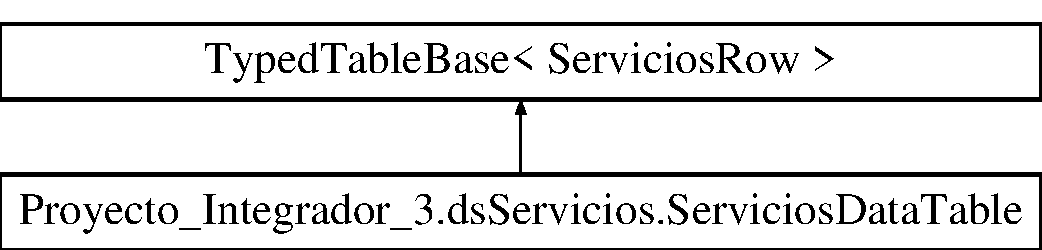
\includegraphics[height=2.000000cm]{dd/d4f/class_proyecto___integrador__3_1_1ds_servicios_1_1_servicios_data_table}
\end{center}
\end{figure}
\subsection*{Métodos públicos}
\begin{DoxyCompactItemize}
\item 
\hyperlink{class_proyecto___integrador__3_1_1ds_servicios_1_1_servicios_data_table_af447c5ce011f17746ed48380ef8f5373}{Servicios\-Data\-Table} ()
\item 
void \hyperlink{class_proyecto___integrador__3_1_1ds_servicios_1_1_servicios_data_table_a7974644d9b5b0b8a5984af24e16700bb}{Add\-Servicios\-Row} (\hyperlink{class_proyecto___integrador__3_1_1ds_servicios_1_1_servicios_row}{Servicios\-Row} row)
\item 
\hyperlink{class_proyecto___integrador__3_1_1ds_servicios_1_1_servicios_row}{Servicios\-Row} \hyperlink{class_proyecto___integrador__3_1_1ds_servicios_1_1_servicios_data_table_ad1be2ae4d234bb0b02c800b641a588d3}{Add\-Servicios\-Row} (string tipo\-Usuario, System.\-Guid unidad, System.\-Guid usuario, System.\-Date\-Time fecha)
\item 
\hyperlink{class_proyecto___integrador__3_1_1ds_servicios_1_1_servicios_row}{Servicios\-Row} \hyperlink{class_proyecto___integrador__3_1_1ds_servicios_1_1_servicios_data_table_a3b9b5f243557e8678068d79c90098010}{Find\-Byid} (long id)
\item 
override \\*
global\-::\-System.\-Data.\-Data\-Table \hyperlink{class_proyecto___integrador__3_1_1ds_servicios_1_1_servicios_data_table_a18c623c7de1cbb4a820376247c4cc80c}{Clone} ()
\item 
\hyperlink{class_proyecto___integrador__3_1_1ds_servicios_1_1_servicios_row}{Servicios\-Row} \hyperlink{class_proyecto___integrador__3_1_1ds_servicios_1_1_servicios_data_table_acf349fca06c159ff3684420872cd39ef}{New\-Servicios\-Row} ()
\item 
void \hyperlink{class_proyecto___integrador__3_1_1ds_servicios_1_1_servicios_data_table_af3be40086cae340eb21f7bb459fc2fe7}{Remove\-Servicios\-Row} (\hyperlink{class_proyecto___integrador__3_1_1ds_servicios_1_1_servicios_row}{Servicios\-Row} row)
\end{DoxyCompactItemize}
\subsection*{Métodos públicos estáticos}
\begin{DoxyCompactItemize}
\item 
static \\*
global\-::\-System.\-Xml.\-Schema.\-Xml\-Schema\-Complex\-Type \hyperlink{class_proyecto___integrador__3_1_1ds_servicios_1_1_servicios_data_table_a98f4a20812c3720bf15930302ee8a47a}{Get\-Typed\-Table\-Schema} (global\-::\-System.\-Xml.\-Schema.\-Xml\-Schema\-Set xs)
\end{DoxyCompactItemize}
\subsection*{Métodos protegidos}
\begin{DoxyCompactItemize}
\item 
\hyperlink{class_proyecto___integrador__3_1_1ds_servicios_1_1_servicios_data_table_a61948734b917b9601a8c4ba89f257ce1}{Servicios\-Data\-Table} (global\-::\-System.\-Runtime.\-Serialization.\-Serialization\-Info info, global\-::\-System.\-Runtime.\-Serialization.\-Streaming\-Context context)
\item 
override \\*
global\-::\-System.\-Data.\-Data\-Table \hyperlink{class_proyecto___integrador__3_1_1ds_servicios_1_1_servicios_data_table_afa9306495769d23b1be81ff0930b45ac}{Create\-Instance} ()
\item 
override \\*
global\-::\-System.\-Data.\-Data\-Row \hyperlink{class_proyecto___integrador__3_1_1ds_servicios_1_1_servicios_data_table_a06a0bad0e3c2d30b1aa95d1ddac34770}{New\-Row\-From\-Builder} (global\-::\-System.\-Data.\-Data\-Row\-Builder builder)
\item 
override global\-::\-System.\-Type \hyperlink{class_proyecto___integrador__3_1_1ds_servicios_1_1_servicios_data_table_aae64e60a790da46a32dd554e53396030}{Get\-Row\-Type} ()
\item 
override void \hyperlink{class_proyecto___integrador__3_1_1ds_servicios_1_1_servicios_data_table_adc98ef75ef60983145f5b52e5e80a23a}{On\-Row\-Changed} (global\-::\-System.\-Data.\-Data\-Row\-Change\-Event\-Args e)
\item 
override void \hyperlink{class_proyecto___integrador__3_1_1ds_servicios_1_1_servicios_data_table_ab00bb6b8cb1debbe995bfced0135b57c}{On\-Row\-Changing} (global\-::\-System.\-Data.\-Data\-Row\-Change\-Event\-Args e)
\item 
override void \hyperlink{class_proyecto___integrador__3_1_1ds_servicios_1_1_servicios_data_table_a4ed7e2ef073e09442707667d741ade90}{On\-Row\-Deleted} (global\-::\-System.\-Data.\-Data\-Row\-Change\-Event\-Args e)
\item 
override void \hyperlink{class_proyecto___integrador__3_1_1ds_servicios_1_1_servicios_data_table_ad06d230daed647e51aaf757b7429127f}{On\-Row\-Deleting} (global\-::\-System.\-Data.\-Data\-Row\-Change\-Event\-Args e)
\end{DoxyCompactItemize}
\subsection*{Funciones del 'package'}
\begin{DoxyCompactItemize}
\item 
\hyperlink{class_proyecto___integrador__3_1_1ds_servicios_1_1_servicios_data_table_a3b5fd9102d3638f916385c186a16d6b4}{Servicios\-Data\-Table} (global\-::\-System.\-Data.\-Data\-Table table)
\item 
void \hyperlink{class_proyecto___integrador__3_1_1ds_servicios_1_1_servicios_data_table_a96f02be0920a068ba412f0eb22ddeae6}{Init\-Vars} ()
\end{DoxyCompactItemize}
\subsection*{Propiedades}
\begin{DoxyCompactItemize}
\item 
global\-::\-System.\-Data.\-Data\-Column \hyperlink{class_proyecto___integrador__3_1_1ds_servicios_1_1_servicios_data_table_a238b98b486c4eb6077f5eb1d26596f26}{id\-Column}\hspace{0.3cm}{\ttfamily  \mbox{[}get\mbox{]}}
\item 
global\-::\-System.\-Data.\-Data\-Column \hyperlink{class_proyecto___integrador__3_1_1ds_servicios_1_1_servicios_data_table_a3ce967e456559fdf973c0efc3b70df96}{tipo\-Usuario\-Column}\hspace{0.3cm}{\ttfamily  \mbox{[}get\mbox{]}}
\item 
global\-::\-System.\-Data.\-Data\-Column \hyperlink{class_proyecto___integrador__3_1_1ds_servicios_1_1_servicios_data_table_ab0e7d5e73c91967ce47805cbefda5db3}{unidad\-Column}\hspace{0.3cm}{\ttfamily  \mbox{[}get\mbox{]}}
\item 
global\-::\-System.\-Data.\-Data\-Column \hyperlink{class_proyecto___integrador__3_1_1ds_servicios_1_1_servicios_data_table_ad22d89a1b9164d0edfee2ab6580bd23a}{usuario\-Column}\hspace{0.3cm}{\ttfamily  \mbox{[}get\mbox{]}}
\item 
global\-::\-System.\-Data.\-Data\-Column \hyperlink{class_proyecto___integrador__3_1_1ds_servicios_1_1_servicios_data_table_afc3e8d1e9b39b8a278418310fadc37e1}{fecha\-Column}\hspace{0.3cm}{\ttfamily  \mbox{[}get\mbox{]}}
\item 
int \hyperlink{class_proyecto___integrador__3_1_1ds_servicios_1_1_servicios_data_table_a2e0a353b5ce0c1a3718e78927b5a180c}{Count}\hspace{0.3cm}{\ttfamily  \mbox{[}get\mbox{]}}
\item 
\hyperlink{class_proyecto___integrador__3_1_1ds_servicios_1_1_servicios_row}{Servicios\-Row} \hyperlink{class_proyecto___integrador__3_1_1ds_servicios_1_1_servicios_data_table_a24dd699ba58bb68edc2ca72efa463890}{this\mbox{[}int index\mbox{]}}\hspace{0.3cm}{\ttfamily  \mbox{[}get\mbox{]}}
\end{DoxyCompactItemize}
\subsection*{Eventos}
\begin{DoxyCompactItemize}
\item 
\hyperlink{class_proyecto___integrador__3_1_1ds_servicios_a12a7c95915227392e001d214be4c6c58}{Servicios\-Row\-Change\-Event\-Handler} \hyperlink{class_proyecto___integrador__3_1_1ds_servicios_1_1_servicios_data_table_ab12bdec8a4cc5c92777d020c5f26cb10}{Servicios\-Row\-Changing}
\item 
\hyperlink{class_proyecto___integrador__3_1_1ds_servicios_a12a7c95915227392e001d214be4c6c58}{Servicios\-Row\-Change\-Event\-Handler} \hyperlink{class_proyecto___integrador__3_1_1ds_servicios_1_1_servicios_data_table_a0e8a3232436341c5724f8eb74ecd976d}{Servicios\-Row\-Changed}
\item 
\hyperlink{class_proyecto___integrador__3_1_1ds_servicios_a12a7c95915227392e001d214be4c6c58}{Servicios\-Row\-Change\-Event\-Handler} \hyperlink{class_proyecto___integrador__3_1_1ds_servicios_1_1_servicios_data_table_a59d056a91ad2ab4905fbe239ff440f9d}{Servicios\-Row\-Deleting}
\item 
\hyperlink{class_proyecto___integrador__3_1_1ds_servicios_a12a7c95915227392e001d214be4c6c58}{Servicios\-Row\-Change\-Event\-Handler} \hyperlink{class_proyecto___integrador__3_1_1ds_servicios_1_1_servicios_data_table_a7b2809ac1c63557531a1ae77eceb8805}{Servicios\-Row\-Deleted}
\end{DoxyCompactItemize}
\subsection*{Métodos privados}
\begin{DoxyCompactItemize}
\item 
void \hyperlink{class_proyecto___integrador__3_1_1ds_servicios_1_1_servicios_data_table_a0e603fcb88e1b87c41b87693443ee7f5}{Init\-Class} ()
\end{DoxyCompactItemize}
\subsection*{Atributos privados}
\begin{DoxyCompactItemize}
\item 
global\-::\-System.\-Data.\-Data\-Column \hyperlink{class_proyecto___integrador__3_1_1ds_servicios_1_1_servicios_data_table_a42ed0070aba427354954b37e5955b03b}{columnid}
\item 
global\-::\-System.\-Data.\-Data\-Column \hyperlink{class_proyecto___integrador__3_1_1ds_servicios_1_1_servicios_data_table_ae6e9f606645938b441b38d9c7889971f}{columntipo\-Usuario}
\item 
global\-::\-System.\-Data.\-Data\-Column \hyperlink{class_proyecto___integrador__3_1_1ds_servicios_1_1_servicios_data_table_a3b6ef8814cd3226485969d0a1e3900d3}{columnunidad}
\item 
global\-::\-System.\-Data.\-Data\-Column \hyperlink{class_proyecto___integrador__3_1_1ds_servicios_1_1_servicios_data_table_a528b90d784325ac1cebec3c973dcd0e4}{columnusuario}
\item 
global\-::\-System.\-Data.\-Data\-Column \hyperlink{class_proyecto___integrador__3_1_1ds_servicios_1_1_servicios_data_table_a959f072e2c0689f46c30f9bc31b2cf16}{columnfecha}
\end{DoxyCompactItemize}


\subsection{Descripción detallada}
Represents the strongly named Data\-Table class. 

/summary$>$ 

Definición en la línea 280 del archivo ds\-Servicios.\-Designer.\-cs.



\subsection{Documentación del constructor y destructor}
\hypertarget{class_proyecto___integrador__3_1_1ds_servicios_1_1_servicios_data_table_af447c5ce011f17746ed48380ef8f5373}{\index{Proyecto\-\_\-\-Integrador\-\_\-3\-::ds\-Servicios\-::\-Servicios\-Data\-Table@{Proyecto\-\_\-\-Integrador\-\_\-3\-::ds\-Servicios\-::\-Servicios\-Data\-Table}!Servicios\-Data\-Table@{Servicios\-Data\-Table}}
\index{Servicios\-Data\-Table@{Servicios\-Data\-Table}!Proyecto_Integrador_3::dsServicios::ServiciosDataTable@{Proyecto\-\_\-\-Integrador\-\_\-3\-::ds\-Servicios\-::\-Servicios\-Data\-Table}}
\subsubsection[{Servicios\-Data\-Table}]{\setlength{\rightskip}{0pt plus 5cm}Proyecto\-\_\-\-Integrador\-\_\-3.\-ds\-Servicios.\-Servicios\-Data\-Table.\-Servicios\-Data\-Table (
\begin{DoxyParamCaption}
{}
\end{DoxyParamCaption}
)\hspace{0.3cm}{\ttfamily [inline]}}}\label{class_proyecto___integrador__3_1_1ds_servicios_1_1_servicios_data_table_af447c5ce011f17746ed48380ef8f5373}


Definición en la línea 294 del archivo ds\-Servicios.\-Designer.\-cs.


\begin{DoxyCode}
294                                         \{
295                 this.TableName = \textcolor{stringliteral}{"Servicios"};
296                 this.BeginInit();
297                 this.\hyperlink{class_proyecto___integrador__3_1_1ds_servicios_1_1_servicios_data_table_a0e603fcb88e1b87c41b87693443ee7f5}{InitClass}();
298                 this.EndInit();
299             \}
\end{DoxyCode}
\hypertarget{class_proyecto___integrador__3_1_1ds_servicios_1_1_servicios_data_table_a3b5fd9102d3638f916385c186a16d6b4}{\index{Proyecto\-\_\-\-Integrador\-\_\-3\-::ds\-Servicios\-::\-Servicios\-Data\-Table@{Proyecto\-\_\-\-Integrador\-\_\-3\-::ds\-Servicios\-::\-Servicios\-Data\-Table}!Servicios\-Data\-Table@{Servicios\-Data\-Table}}
\index{Servicios\-Data\-Table@{Servicios\-Data\-Table}!Proyecto_Integrador_3::dsServicios::ServiciosDataTable@{Proyecto\-\_\-\-Integrador\-\_\-3\-::ds\-Servicios\-::\-Servicios\-Data\-Table}}
\subsubsection[{Servicios\-Data\-Table}]{\setlength{\rightskip}{0pt plus 5cm}Proyecto\-\_\-\-Integrador\-\_\-3.\-ds\-Servicios.\-Servicios\-Data\-Table.\-Servicios\-Data\-Table (
\begin{DoxyParamCaption}
\item[{global\-::\-System.\-Data.\-Data\-Table}]{table}
\end{DoxyParamCaption}
)\hspace{0.3cm}{\ttfamily [inline]}, {\ttfamily [package]}}}\label{class_proyecto___integrador__3_1_1ds_servicios_1_1_servicios_data_table_a3b5fd9102d3638f916385c186a16d6b4}


Definición en la línea 303 del archivo ds\-Servicios.\-Designer.\-cs.


\begin{DoxyCode}
303                                                                            \{
304                 this.TableName = table.TableName;
305                 \textcolor{keywordflow}{if} ((table.CaseSensitive != table.DataSet.CaseSensitive)) \{
306                     this.CaseSensitive = table.CaseSensitive;
307                 \}
308                 \textcolor{keywordflow}{if} ((table.Locale.ToString() != table.DataSet.Locale.ToString())) \{
309                     this.Locale = table.Locale;
310                 \}
311                 \textcolor{keywordflow}{if} ((table.Namespace != table.DataSet.Namespace)) \{
312                     this.Namespace = table.Namespace;
313                 \}
314                 this.Prefix = table.Prefix;
315                 this.MinimumCapacity = table.MinimumCapacity;
316             \}
\end{DoxyCode}
\hypertarget{class_proyecto___integrador__3_1_1ds_servicios_1_1_servicios_data_table_a61948734b917b9601a8c4ba89f257ce1}{\index{Proyecto\-\_\-\-Integrador\-\_\-3\-::ds\-Servicios\-::\-Servicios\-Data\-Table@{Proyecto\-\_\-\-Integrador\-\_\-3\-::ds\-Servicios\-::\-Servicios\-Data\-Table}!Servicios\-Data\-Table@{Servicios\-Data\-Table}}
\index{Servicios\-Data\-Table@{Servicios\-Data\-Table}!Proyecto_Integrador_3::dsServicios::ServiciosDataTable@{Proyecto\-\_\-\-Integrador\-\_\-3\-::ds\-Servicios\-::\-Servicios\-Data\-Table}}
\subsubsection[{Servicios\-Data\-Table}]{\setlength{\rightskip}{0pt plus 5cm}Proyecto\-\_\-\-Integrador\-\_\-3.\-ds\-Servicios.\-Servicios\-Data\-Table.\-Servicios\-Data\-Table (
\begin{DoxyParamCaption}
\item[{global\-::\-System.\-Runtime.\-Serialization.\-Serialization\-Info}]{info, }
\item[{global\-::\-System.\-Runtime.\-Serialization.\-Streaming\-Context}]{context}
\end{DoxyParamCaption}
)\hspace{0.3cm}{\ttfamily [inline]}, {\ttfamily [protected]}}}\label{class_proyecto___integrador__3_1_1ds_servicios_1_1_servicios_data_table_a61948734b917b9601a8c4ba89f257ce1}


Definición en la línea 320 del archivo ds\-Servicios.\-Designer.\-cs.


\begin{DoxyCode}
320                                                                                                            
                                                            : 
321                     base(info, context) \{
322                 this.\hyperlink{class_proyecto___integrador__3_1_1ds_servicios_1_1_servicios_data_table_a96f02be0920a068ba412f0eb22ddeae6}{InitVars}();
323             \}
\end{DoxyCode}


\subsection{Documentación de las funciones miembro}
\hypertarget{class_proyecto___integrador__3_1_1ds_servicios_1_1_servicios_data_table_a7974644d9b5b0b8a5984af24e16700bb}{\index{Proyecto\-\_\-\-Integrador\-\_\-3\-::ds\-Servicios\-::\-Servicios\-Data\-Table@{Proyecto\-\_\-\-Integrador\-\_\-3\-::ds\-Servicios\-::\-Servicios\-Data\-Table}!Add\-Servicios\-Row@{Add\-Servicios\-Row}}
\index{Add\-Servicios\-Row@{Add\-Servicios\-Row}!Proyecto_Integrador_3::dsServicios::ServiciosDataTable@{Proyecto\-\_\-\-Integrador\-\_\-3\-::ds\-Servicios\-::\-Servicios\-Data\-Table}}
\subsubsection[{Add\-Servicios\-Row}]{\setlength{\rightskip}{0pt plus 5cm}void Proyecto\-\_\-\-Integrador\-\_\-3.\-ds\-Servicios.\-Servicios\-Data\-Table.\-Add\-Servicios\-Row (
\begin{DoxyParamCaption}
\item[{{\bf Servicios\-Row}}]{row}
\end{DoxyParamCaption}
)\hspace{0.3cm}{\ttfamily [inline]}}}\label{class_proyecto___integrador__3_1_1ds_servicios_1_1_servicios_data_table_a7974644d9b5b0b8a5984af24e16700bb}


Definición en la línea 396 del archivo ds\-Servicios.\-Designer.\-cs.


\begin{DoxyCode}
396                                                           \{
397                 this.Rows.Add(row);
398             \}
\end{DoxyCode}
\hypertarget{class_proyecto___integrador__3_1_1ds_servicios_1_1_servicios_data_table_ad1be2ae4d234bb0b02c800b641a588d3}{\index{Proyecto\-\_\-\-Integrador\-\_\-3\-::ds\-Servicios\-::\-Servicios\-Data\-Table@{Proyecto\-\_\-\-Integrador\-\_\-3\-::ds\-Servicios\-::\-Servicios\-Data\-Table}!Add\-Servicios\-Row@{Add\-Servicios\-Row}}
\index{Add\-Servicios\-Row@{Add\-Servicios\-Row}!Proyecto_Integrador_3::dsServicios::ServiciosDataTable@{Proyecto\-\_\-\-Integrador\-\_\-3\-::ds\-Servicios\-::\-Servicios\-Data\-Table}}
\subsubsection[{Add\-Servicios\-Row}]{\setlength{\rightskip}{0pt plus 5cm}{\bf Servicios\-Row} Proyecto\-\_\-\-Integrador\-\_\-3.\-ds\-Servicios.\-Servicios\-Data\-Table.\-Add\-Servicios\-Row (
\begin{DoxyParamCaption}
\item[{string}]{tipo\-Usuario, }
\item[{System.\-Guid}]{unidad, }
\item[{System.\-Guid}]{usuario, }
\item[{System.\-Date\-Time}]{fecha}
\end{DoxyParamCaption}
)\hspace{0.3cm}{\ttfamily [inline]}}}\label{class_proyecto___integrador__3_1_1ds_servicios_1_1_servicios_data_table_ad1be2ae4d234bb0b02c800b641a588d3}


Definición en la línea 402 del archivo ds\-Servicios.\-Designer.\-cs.


\begin{DoxyCode}
402                                                                                                            
                               \{
403                 \hyperlink{_servicios_populator_8cs_a4fedc76bdc7093e47c2dfca7a41b823b}{ServiciosRow} rowServiciosRow = ((\hyperlink{_servicios_populator_8cs_a4fedc76bdc7093e47c2dfca7a41b823b}{ServiciosRow})(this.NewRow()));
404                 \textcolor{keywordtype}{object}[] columnValuesArray = \textcolor{keyword}{new} \textcolor{keywordtype}{object}[] \{
405                         null,
406                         tipoUsuario,
407                         unidad,
408                         usuario,
409                         fecha\};
410                 rowServiciosRow.ItemArray = columnValuesArray;
411                 this.Rows.Add(rowServiciosRow);
412                 \textcolor{keywordflow}{return} rowServiciosRow;
413             \}
\end{DoxyCode}
\hypertarget{class_proyecto___integrador__3_1_1ds_servicios_1_1_servicios_data_table_a18c623c7de1cbb4a820376247c4cc80c}{\index{Proyecto\-\_\-\-Integrador\-\_\-3\-::ds\-Servicios\-::\-Servicios\-Data\-Table@{Proyecto\-\_\-\-Integrador\-\_\-3\-::ds\-Servicios\-::\-Servicios\-Data\-Table}!Clone@{Clone}}
\index{Clone@{Clone}!Proyecto_Integrador_3::dsServicios::ServiciosDataTable@{Proyecto\-\_\-\-Integrador\-\_\-3\-::ds\-Servicios\-::\-Servicios\-Data\-Table}}
\subsubsection[{Clone}]{\setlength{\rightskip}{0pt plus 5cm}override global.\-System.\-Data.\-Data\-Table Proyecto\-\_\-\-Integrador\-\_\-3.\-ds\-Servicios.\-Servicios\-Data\-Table.\-Clone (
\begin{DoxyParamCaption}
{}
\end{DoxyParamCaption}
)\hspace{0.3cm}{\ttfamily [inline]}}}\label{class_proyecto___integrador__3_1_1ds_servicios_1_1_servicios_data_table_a18c623c7de1cbb4a820376247c4cc80c}


Definición en la línea 424 del archivo ds\-Servicios.\-Designer.\-cs.


\begin{DoxyCode}
424                                                                 \{
425                 \hyperlink{class_proyecto___integrador__3_1_1ds_servicios_1_1_servicios_data_table_af447c5ce011f17746ed48380ef8f5373}{ServiciosDataTable} cln = ((\hyperlink{class_proyecto___integrador__3_1_1ds_servicios_1_1_servicios_data_table_af447c5ce011f17746ed48380ef8f5373}{ServiciosDataTable})(base.
      Clone()));
426                 cln.InitVars();
427                 \textcolor{keywordflow}{return} cln;
428             \}
\end{DoxyCode}
\hypertarget{class_proyecto___integrador__3_1_1ds_servicios_1_1_servicios_data_table_afa9306495769d23b1be81ff0930b45ac}{\index{Proyecto\-\_\-\-Integrador\-\_\-3\-::ds\-Servicios\-::\-Servicios\-Data\-Table@{Proyecto\-\_\-\-Integrador\-\_\-3\-::ds\-Servicios\-::\-Servicios\-Data\-Table}!Create\-Instance@{Create\-Instance}}
\index{Create\-Instance@{Create\-Instance}!Proyecto_Integrador_3::dsServicios::ServiciosDataTable@{Proyecto\-\_\-\-Integrador\-\_\-3\-::ds\-Servicios\-::\-Servicios\-Data\-Table}}
\subsubsection[{Create\-Instance}]{\setlength{\rightskip}{0pt plus 5cm}override global.\-System.\-Data.\-Data\-Table Proyecto\-\_\-\-Integrador\-\_\-3.\-ds\-Servicios.\-Servicios\-Data\-Table.\-Create\-Instance (
\begin{DoxyParamCaption}
{}
\end{DoxyParamCaption}
)\hspace{0.3cm}{\ttfamily [inline]}, {\ttfamily [protected]}}}\label{class_proyecto___integrador__3_1_1ds_servicios_1_1_servicios_data_table_afa9306495769d23b1be81ff0930b45ac}


Definición en la línea 432 del archivo ds\-Servicios.\-Designer.\-cs.


\begin{DoxyCode}
432                                                                             \{
433                 \textcolor{keywordflow}{return} \textcolor{keyword}{new} \hyperlink{class_proyecto___integrador__3_1_1ds_servicios_1_1_servicios_data_table_af447c5ce011f17746ed48380ef8f5373}{ServiciosDataTable}();
434             \}
\end{DoxyCode}
\hypertarget{class_proyecto___integrador__3_1_1ds_servicios_1_1_servicios_data_table_a3b9b5f243557e8678068d79c90098010}{\index{Proyecto\-\_\-\-Integrador\-\_\-3\-::ds\-Servicios\-::\-Servicios\-Data\-Table@{Proyecto\-\_\-\-Integrador\-\_\-3\-::ds\-Servicios\-::\-Servicios\-Data\-Table}!Find\-Byid@{Find\-Byid}}
\index{Find\-Byid@{Find\-Byid}!Proyecto_Integrador_3::dsServicios::ServiciosDataTable@{Proyecto\-\_\-\-Integrador\-\_\-3\-::ds\-Servicios\-::\-Servicios\-Data\-Table}}
\subsubsection[{Find\-Byid}]{\setlength{\rightskip}{0pt plus 5cm}{\bf Servicios\-Row} Proyecto\-\_\-\-Integrador\-\_\-3.\-ds\-Servicios.\-Servicios\-Data\-Table.\-Find\-Byid (
\begin{DoxyParamCaption}
\item[{long}]{id}
\end{DoxyParamCaption}
)\hspace{0.3cm}{\ttfamily [inline]}}}\label{class_proyecto___integrador__3_1_1ds_servicios_1_1_servicios_data_table_a3b9b5f243557e8678068d79c90098010}


Definición en la línea 417 del archivo ds\-Servicios.\-Designer.\-cs.


\begin{DoxyCode}
417                                                   \{
418                 \textcolor{keywordflow}{return} ((\hyperlink{_servicios_populator_8cs_a4fedc76bdc7093e47c2dfca7a41b823b}{ServiciosRow})(this.Rows.Find(\textcolor{keyword}{new} \textcolor{keywordtype}{object}[] \{
419                             \textcolor{keywordtype}{id}\})));
420             \}
\end{DoxyCode}
\hypertarget{class_proyecto___integrador__3_1_1ds_servicios_1_1_servicios_data_table_aae64e60a790da46a32dd554e53396030}{\index{Proyecto\-\_\-\-Integrador\-\_\-3\-::ds\-Servicios\-::\-Servicios\-Data\-Table@{Proyecto\-\_\-\-Integrador\-\_\-3\-::ds\-Servicios\-::\-Servicios\-Data\-Table}!Get\-Row\-Type@{Get\-Row\-Type}}
\index{Get\-Row\-Type@{Get\-Row\-Type}!Proyecto_Integrador_3::dsServicios::ServiciosDataTable@{Proyecto\-\_\-\-Integrador\-\_\-3\-::ds\-Servicios\-::\-Servicios\-Data\-Table}}
\subsubsection[{Get\-Row\-Type}]{\setlength{\rightskip}{0pt plus 5cm}override global.\-System.\-Type Proyecto\-\_\-\-Integrador\-\_\-3.\-ds\-Servicios.\-Servicios\-Data\-Table.\-Get\-Row\-Type (
\begin{DoxyParamCaption}
{}
\end{DoxyParamCaption}
)\hspace{0.3cm}{\ttfamily [inline]}, {\ttfamily [protected]}}}\label{class_proyecto___integrador__3_1_1ds_servicios_1_1_servicios_data_table_aae64e60a790da46a32dd554e53396030}


Definición en la línea 488 del archivo ds\-Servicios.\-Designer.\-cs.


\begin{DoxyCode}
488                                                               \{
489                 \textcolor{keywordflow}{return} typeof(\hyperlink{_servicios_populator_8cs_a4fedc76bdc7093e47c2dfca7a41b823b}{ServiciosRow});
490             \}
\end{DoxyCode}
\hypertarget{class_proyecto___integrador__3_1_1ds_servicios_1_1_servicios_data_table_a98f4a20812c3720bf15930302ee8a47a}{\index{Proyecto\-\_\-\-Integrador\-\_\-3\-::ds\-Servicios\-::\-Servicios\-Data\-Table@{Proyecto\-\_\-\-Integrador\-\_\-3\-::ds\-Servicios\-::\-Servicios\-Data\-Table}!Get\-Typed\-Table\-Schema@{Get\-Typed\-Table\-Schema}}
\index{Get\-Typed\-Table\-Schema@{Get\-Typed\-Table\-Schema}!Proyecto_Integrador_3::dsServicios::ServiciosDataTable@{Proyecto\-\_\-\-Integrador\-\_\-3\-::ds\-Servicios\-::\-Servicios\-Data\-Table}}
\subsubsection[{Get\-Typed\-Table\-Schema}]{\setlength{\rightskip}{0pt plus 5cm}static global.\-System.\-Xml.\-Schema.\-Xml\-Schema\-Complex\-Type Proyecto\-\_\-\-Integrador\-\_\-3.\-ds\-Servicios.\-Servicios\-Data\-Table.\-Get\-Typed\-Table\-Schema (
\begin{DoxyParamCaption}
\item[{global\-::\-System.\-Xml.\-Schema.\-Xml\-Schema\-Set}]{xs}
\end{DoxyParamCaption}
)\hspace{0.3cm}{\ttfamily [inline]}, {\ttfamily [static]}}}\label{class_proyecto___integrador__3_1_1ds_servicios_1_1_servicios_data_table_a98f4a20812c3720bf15930302ee8a47a}


Definición en la línea 536 del archivo ds\-Servicios.\-Designer.\-cs.


\begin{DoxyCode}
536                                                                                                            
                               \{
537                 global::System.Xml.Schema.XmlSchemaComplexType type = \textcolor{keyword}{new} global::System.Xml.Schema.
      XmlSchemaComplexType();
538                 global::System.Xml.Schema.XmlSchemaSequence sequence = \textcolor{keyword}{new} global::System.Xml.Schema.
      XmlSchemaSequence();
539                 \hyperlink{class_proyecto___integrador__3_1_1ds_servicios_a0734e62bba29ca7515ed72f2aee94662}{dsServicios} ds = \textcolor{keyword}{new} \hyperlink{class_proyecto___integrador__3_1_1ds_servicios_a0734e62bba29ca7515ed72f2aee94662}{dsServicios}();
540                 global::System.Xml.Schema.XmlSchemaAny any1 = \textcolor{keyword}{new} global::System.Xml.Schema.XmlSchemaAny();
541                 any1.Namespace = \textcolor{stringliteral}{"http://www.w3.org/2001/XMLSchema"};
542                 any1.MinOccurs = \textcolor{keyword}{new} decimal(0);
543                 any1.MaxOccurs = decimal.MaxValue;
544                 any1.ProcessContents = global::System.Xml.Schema.XmlSchemaContentProcessing.Lax;
545                 sequence.Items.Add(any1);
546                 global::System.Xml.Schema.XmlSchemaAny any2 = \textcolor{keyword}{new} global::System.Xml.Schema.XmlSchemaAny();
547                 any2.Namespace = \textcolor{stringliteral}{"urn:schemas-microsoft-com:xml-diffgram-v1"};
548                 any2.MinOccurs = \textcolor{keyword}{new} decimal(1);
549                 any2.ProcessContents = global::System.Xml.Schema.XmlSchemaContentProcessing.Lax;
550                 sequence.Items.Add(any2);
551                 global::System.Xml.Schema.XmlSchemaAttribute attribute1 = \textcolor{keyword}{new} global::System.Xml.Schema.
      XmlSchemaAttribute();
552                 attribute1.Name = \textcolor{stringliteral}{"namespace"};
553                 attribute1.FixedValue = ds.Namespace;
554                 type.Attributes.Add(attribute1);
555                 global::System.Xml.Schema.XmlSchemaAttribute attribute2 = \textcolor{keyword}{new} global::System.Xml.Schema.
      XmlSchemaAttribute();
556                 attribute2.Name = \textcolor{stringliteral}{"tableTypeName"};
557                 attribute2.FixedValue = \textcolor{stringliteral}{"ServiciosDataTable"};
558                 type.Attributes.Add(attribute2);
559                 type.Particle = sequence;
560                 global::System.Xml.Schema.XmlSchema dsSchema = ds.GetSchemaSerializable();
561                 \textcolor{keywordflow}{if} (xs.Contains(dsSchema.TargetNamespace)) \{
562                     global::System.IO.MemoryStream s1 = \textcolor{keyword}{new} global::System.IO.MemoryStream();
563                     global::System.IO.MemoryStream s2 = \textcolor{keyword}{new} global::System.IO.MemoryStream();
564                     \textcolor{keywordflow}{try} \{
565                         global::System.Xml.Schema.XmlSchema schema = null;
566                         dsSchema.Write(s1);
567                         \textcolor{keywordflow}{for} (global::System.Collections.IEnumerator schemas = xs.Schemas(dsSchema.
      TargetNamespace).GetEnumerator(); schemas.MoveNext(); ) \{
568                             schema = ((global::System.Xml.Schema.XmlSchema)(schemas.Current));
569                             s2.SetLength(0);
570                             schema.Write(s2);
571                             \textcolor{keywordflow}{if} ((s1.Length == s2.Length)) \{
572                                 s1.Position = 0;
573                                 s2.Position = 0;
574                                 \textcolor{keywordflow}{for} (; ((s1.Position != s1.Length) 
575                                             && (s1.ReadByte() == s2.ReadByte())); ) \{
576                                     ;
577                                 \}
578                                 \textcolor{keywordflow}{if} ((s1.Position == s1.Length)) \{
579                                     \textcolor{keywordflow}{return} type;
580                                 \}
581                             \}
582                         \}
583                     \}
584                     \textcolor{keywordflow}{finally} \{
585                         \textcolor{keywordflow}{if} ((s1 != null)) \{
586                             s1.Close();
587                         \}
588                         \textcolor{keywordflow}{if} ((s2 != null)) \{
589                             s2.Close();
590                         \}
591                     \}
592                 \}
593                 xs.Add(dsSchema);
594                 \textcolor{keywordflow}{return} type;
595             \}
\end{DoxyCode}
\hypertarget{class_proyecto___integrador__3_1_1ds_servicios_1_1_servicios_data_table_a0e603fcb88e1b87c41b87693443ee7f5}{\index{Proyecto\-\_\-\-Integrador\-\_\-3\-::ds\-Servicios\-::\-Servicios\-Data\-Table@{Proyecto\-\_\-\-Integrador\-\_\-3\-::ds\-Servicios\-::\-Servicios\-Data\-Table}!Init\-Class@{Init\-Class}}
\index{Init\-Class@{Init\-Class}!Proyecto_Integrador_3::dsServicios::ServiciosDataTable@{Proyecto\-\_\-\-Integrador\-\_\-3\-::ds\-Servicios\-::\-Servicios\-Data\-Table}}
\subsubsection[{Init\-Class}]{\setlength{\rightskip}{0pt plus 5cm}void Proyecto\-\_\-\-Integrador\-\_\-3.\-ds\-Servicios.\-Servicios\-Data\-Table.\-Init\-Class (
\begin{DoxyParamCaption}
{}
\end{DoxyParamCaption}
)\hspace{0.3cm}{\ttfamily [inline]}, {\ttfamily [private]}}}\label{class_proyecto___integrador__3_1_1ds_servicios_1_1_servicios_data_table_a0e603fcb88e1b87c41b87693443ee7f5}


Definición en la línea 448 del archivo ds\-Servicios.\-Designer.\-cs.


\begin{DoxyCode}
448                                      \{
449                 this.\hyperlink{class_proyecto___integrador__3_1_1ds_servicios_1_1_servicios_data_table_a42ed0070aba427354954b37e5955b03b}{columnid} = \textcolor{keyword}{new} global::System.Data.DataColumn(\textcolor{stringliteral}{"id"}, typeof(\textcolor{keywordtype}{long}), null, 
      global::System.Data.MappingType.Element);
450                 base.Columns.Add(this.\hyperlink{class_proyecto___integrador__3_1_1ds_servicios_1_1_servicios_data_table_a42ed0070aba427354954b37e5955b03b}{columnid});
451                 this.\hyperlink{class_proyecto___integrador__3_1_1ds_servicios_1_1_servicios_data_table_ae6e9f606645938b441b38d9c7889971f}{columntipoUsuario} = \textcolor{keyword}{new} global::System.Data.DataColumn(\textcolor{stringliteral}{"tipoUsuario"},
       typeof(\textcolor{keywordtype}{string}), null, global::System.Data.MappingType.Element);
452                 base.Columns.Add(this.\hyperlink{class_proyecto___integrador__3_1_1ds_servicios_1_1_servicios_data_table_ae6e9f606645938b441b38d9c7889971f}{columntipoUsuario});
453                 this.\hyperlink{class_proyecto___integrador__3_1_1ds_servicios_1_1_servicios_data_table_a3b6ef8814cd3226485969d0a1e3900d3}{columnunidad} = \textcolor{keyword}{new} global::System.Data.DataColumn(\textcolor{stringliteral}{"unidad"}, typeof(
      global::System.Guid), null, global::System.Data.MappingType.Element);
454                 base.Columns.Add(this.\hyperlink{class_proyecto___integrador__3_1_1ds_servicios_1_1_servicios_data_table_a3b6ef8814cd3226485969d0a1e3900d3}{columnunidad});
455                 this.\hyperlink{class_proyecto___integrador__3_1_1ds_servicios_1_1_servicios_data_table_a528b90d784325ac1cebec3c973dcd0e4}{columnusuario} = \textcolor{keyword}{new} global::System.Data.DataColumn(\textcolor{stringliteral}{"usuario"}, typeof(
      global::System.Guid), null, global::System.Data.MappingType.Element);
456                 base.Columns.Add(this.\hyperlink{class_proyecto___integrador__3_1_1ds_servicios_1_1_servicios_data_table_a528b90d784325ac1cebec3c973dcd0e4}{columnusuario});
457                 this.\hyperlink{class_proyecto___integrador__3_1_1ds_servicios_1_1_servicios_data_table_a959f072e2c0689f46c30f9bc31b2cf16}{columnfecha} = \textcolor{keyword}{new} global::System.Data.DataColumn(\textcolor{stringliteral}{"fecha"}, typeof(
      global::System.DateTime), null, global::System.Data.MappingType.Element);
458                 base.Columns.Add(this.\hyperlink{class_proyecto___integrador__3_1_1ds_servicios_1_1_servicios_data_table_a959f072e2c0689f46c30f9bc31b2cf16}{columnfecha});
459                 this.Constraints.Add(\textcolor{keyword}{new} global::System.Data.UniqueConstraint(\textcolor{stringliteral}{"Constraint1"}, \textcolor{keyword}{new} 
      global::System.Data.DataColumn[] \{
460                                 \textcolor{keyword}{this}.columnid\}, \textcolor{keyword}{true}));
461                 this.\hyperlink{class_proyecto___integrador__3_1_1ds_servicios_1_1_servicios_data_table_a42ed0070aba427354954b37e5955b03b}{columnid}.AutoIncrement = \textcolor{keyword}{true};
462                 this.\hyperlink{class_proyecto___integrador__3_1_1ds_servicios_1_1_servicios_data_table_a42ed0070aba427354954b37e5955b03b}{columnid}.AutoIncrementSeed = 1;
463                 this.\hyperlink{class_proyecto___integrador__3_1_1ds_servicios_1_1_servicios_data_table_a42ed0070aba427354954b37e5955b03b}{columnid}.AllowDBNull = \textcolor{keyword}{false};
464                 this.\hyperlink{class_proyecto___integrador__3_1_1ds_servicios_1_1_servicios_data_table_a42ed0070aba427354954b37e5955b03b}{columnid}.ReadOnly = \textcolor{keyword}{true};
465                 this.\hyperlink{class_proyecto___integrador__3_1_1ds_servicios_1_1_servicios_data_table_a42ed0070aba427354954b37e5955b03b}{columnid}.Unique = \textcolor{keyword}{true};
466                 this.\hyperlink{class_proyecto___integrador__3_1_1ds_servicios_1_1_servicios_data_table_ae6e9f606645938b441b38d9c7889971f}{columntipoUsuario}.AllowDBNull = \textcolor{keyword}{false};
467                 this.\hyperlink{class_proyecto___integrador__3_1_1ds_servicios_1_1_servicios_data_table_ae6e9f606645938b441b38d9c7889971f}{columntipoUsuario}.DefaultValue = ((string)(\textcolor{stringliteral}{"1"}));
468                 this.\hyperlink{class_proyecto___integrador__3_1_1ds_servicios_1_1_servicios_data_table_ae6e9f606645938b441b38d9c7889971f}{columntipoUsuario}.MaxLength = 1;
469                 this.\hyperlink{class_proyecto___integrador__3_1_1ds_servicios_1_1_servicios_data_table_a3b6ef8814cd3226485969d0a1e3900d3}{columnunidad}.AllowDBNull = \textcolor{keyword}{false};
470                 this.\hyperlink{class_proyecto___integrador__3_1_1ds_servicios_1_1_servicios_data_table_a528b90d784325ac1cebec3c973dcd0e4}{columnusuario}.AllowDBNull = \textcolor{keyword}{false};
471                 this.\hyperlink{class_proyecto___integrador__3_1_1ds_servicios_1_1_servicios_data_table_a959f072e2c0689f46c30f9bc31b2cf16}{columnfecha}.AllowDBNull = \textcolor{keyword}{false};
472             \}
\end{DoxyCode}
\hypertarget{class_proyecto___integrador__3_1_1ds_servicios_1_1_servicios_data_table_a96f02be0920a068ba412f0eb22ddeae6}{\index{Proyecto\-\_\-\-Integrador\-\_\-3\-::ds\-Servicios\-::\-Servicios\-Data\-Table@{Proyecto\-\_\-\-Integrador\-\_\-3\-::ds\-Servicios\-::\-Servicios\-Data\-Table}!Init\-Vars@{Init\-Vars}}
\index{Init\-Vars@{Init\-Vars}!Proyecto_Integrador_3::dsServicios::ServiciosDataTable@{Proyecto\-\_\-\-Integrador\-\_\-3\-::ds\-Servicios\-::\-Servicios\-Data\-Table}}
\subsubsection[{Init\-Vars}]{\setlength{\rightskip}{0pt plus 5cm}void Proyecto\-\_\-\-Integrador\-\_\-3.\-ds\-Servicios.\-Servicios\-Data\-Table.\-Init\-Vars (
\begin{DoxyParamCaption}
{}
\end{DoxyParamCaption}
)\hspace{0.3cm}{\ttfamily [inline]}, {\ttfamily [package]}}}\label{class_proyecto___integrador__3_1_1ds_servicios_1_1_servicios_data_table_a96f02be0920a068ba412f0eb22ddeae6}


Definición en la línea 438 del archivo ds\-Servicios.\-Designer.\-cs.


\begin{DoxyCode}
438                                      \{
439                 this.\hyperlink{class_proyecto___integrador__3_1_1ds_servicios_1_1_servicios_data_table_a42ed0070aba427354954b37e5955b03b}{columnid} = base.Columns[\textcolor{stringliteral}{"id"}];
440                 this.\hyperlink{class_proyecto___integrador__3_1_1ds_servicios_1_1_servicios_data_table_ae6e9f606645938b441b38d9c7889971f}{columntipoUsuario} = base.Columns[\textcolor{stringliteral}{"tipoUsuario"}];
441                 this.\hyperlink{class_proyecto___integrador__3_1_1ds_servicios_1_1_servicios_data_table_a3b6ef8814cd3226485969d0a1e3900d3}{columnunidad} = base.Columns[\textcolor{stringliteral}{"unidad"}];
442                 this.\hyperlink{class_proyecto___integrador__3_1_1ds_servicios_1_1_servicios_data_table_a528b90d784325ac1cebec3c973dcd0e4}{columnusuario} = base.Columns[\textcolor{stringliteral}{"usuario"}];
443                 this.\hyperlink{class_proyecto___integrador__3_1_1ds_servicios_1_1_servicios_data_table_a959f072e2c0689f46c30f9bc31b2cf16}{columnfecha} = base.Columns[\textcolor{stringliteral}{"fecha"}];
444             \}
\end{DoxyCode}
\hypertarget{class_proyecto___integrador__3_1_1ds_servicios_1_1_servicios_data_table_a06a0bad0e3c2d30b1aa95d1ddac34770}{\index{Proyecto\-\_\-\-Integrador\-\_\-3\-::ds\-Servicios\-::\-Servicios\-Data\-Table@{Proyecto\-\_\-\-Integrador\-\_\-3\-::ds\-Servicios\-::\-Servicios\-Data\-Table}!New\-Row\-From\-Builder@{New\-Row\-From\-Builder}}
\index{New\-Row\-From\-Builder@{New\-Row\-From\-Builder}!Proyecto_Integrador_3::dsServicios::ServiciosDataTable@{Proyecto\-\_\-\-Integrador\-\_\-3\-::ds\-Servicios\-::\-Servicios\-Data\-Table}}
\subsubsection[{New\-Row\-From\-Builder}]{\setlength{\rightskip}{0pt plus 5cm}override global.\-System.\-Data.\-Data\-Row Proyecto\-\_\-\-Integrador\-\_\-3.\-ds\-Servicios.\-Servicios\-Data\-Table.\-New\-Row\-From\-Builder (
\begin{DoxyParamCaption}
\item[{global\-::\-System.\-Data.\-Data\-Row\-Builder}]{builder}
\end{DoxyParamCaption}
)\hspace{0.3cm}{\ttfamily [inline]}, {\ttfamily [protected]}}}\label{class_proyecto___integrador__3_1_1ds_servicios_1_1_servicios_data_table_a06a0bad0e3c2d30b1aa95d1ddac34770}


Definición en la línea 482 del archivo ds\-Servicios.\-Designer.\-cs.


\begin{DoxyCode}
482                                                                                                            
                \{
483                 \textcolor{keywordflow}{return} \textcolor{keyword}{new} \hyperlink{_servicios_populator_8cs_a4fedc76bdc7093e47c2dfca7a41b823b}{ServiciosRow}(builder);
484             \}
\end{DoxyCode}
\hypertarget{class_proyecto___integrador__3_1_1ds_servicios_1_1_servicios_data_table_acf349fca06c159ff3684420872cd39ef}{\index{Proyecto\-\_\-\-Integrador\-\_\-3\-::ds\-Servicios\-::\-Servicios\-Data\-Table@{Proyecto\-\_\-\-Integrador\-\_\-3\-::ds\-Servicios\-::\-Servicios\-Data\-Table}!New\-Servicios\-Row@{New\-Servicios\-Row}}
\index{New\-Servicios\-Row@{New\-Servicios\-Row}!Proyecto_Integrador_3::dsServicios::ServiciosDataTable@{Proyecto\-\_\-\-Integrador\-\_\-3\-::ds\-Servicios\-::\-Servicios\-Data\-Table}}
\subsubsection[{New\-Servicios\-Row}]{\setlength{\rightskip}{0pt plus 5cm}{\bf Servicios\-Row} Proyecto\-\_\-\-Integrador\-\_\-3.\-ds\-Servicios.\-Servicios\-Data\-Table.\-New\-Servicios\-Row (
\begin{DoxyParamCaption}
{}
\end{DoxyParamCaption}
)\hspace{0.3cm}{\ttfamily [inline]}}}\label{class_proyecto___integrador__3_1_1ds_servicios_1_1_servicios_data_table_acf349fca06c159ff3684420872cd39ef}


Definición en la línea 476 del archivo ds\-Servicios.\-Designer.\-cs.


\begin{DoxyCode}
476                                                   \{
477                 \textcolor{keywordflow}{return} ((\hyperlink{_servicios_populator_8cs_a4fedc76bdc7093e47c2dfca7a41b823b}{ServiciosRow})(this.NewRow()));
478             \}
\end{DoxyCode}
\hypertarget{class_proyecto___integrador__3_1_1ds_servicios_1_1_servicios_data_table_adc98ef75ef60983145f5b52e5e80a23a}{\index{Proyecto\-\_\-\-Integrador\-\_\-3\-::ds\-Servicios\-::\-Servicios\-Data\-Table@{Proyecto\-\_\-\-Integrador\-\_\-3\-::ds\-Servicios\-::\-Servicios\-Data\-Table}!On\-Row\-Changed@{On\-Row\-Changed}}
\index{On\-Row\-Changed@{On\-Row\-Changed}!Proyecto_Integrador_3::dsServicios::ServiciosDataTable@{Proyecto\-\_\-\-Integrador\-\_\-3\-::ds\-Servicios\-::\-Servicios\-Data\-Table}}
\subsubsection[{On\-Row\-Changed}]{\setlength{\rightskip}{0pt plus 5cm}override void Proyecto\-\_\-\-Integrador\-\_\-3.\-ds\-Servicios.\-Servicios\-Data\-Table.\-On\-Row\-Changed (
\begin{DoxyParamCaption}
\item[{global\-::\-System.\-Data.\-Data\-Row\-Change\-Event\-Args}]{e}
\end{DoxyParamCaption}
)\hspace{0.3cm}{\ttfamily [inline]}, {\ttfamily [protected]}}}\label{class_proyecto___integrador__3_1_1ds_servicios_1_1_servicios_data_table_adc98ef75ef60983145f5b52e5e80a23a}


Definición en la línea 494 del archivo ds\-Servicios.\-Designer.\-cs.


\begin{DoxyCode}
494                                                                                              \{
495                 base.OnRowChanged(e);
496                 \textcolor{keywordflow}{if} ((this.\hyperlink{class_proyecto___integrador__3_1_1ds_servicios_1_1_servicios_data_table_a0e8a3232436341c5724f8eb74ecd976d}{ServiciosRowChanged} != null)) \{
497                     this.\hyperlink{class_proyecto___integrador__3_1_1ds_servicios_1_1_servicios_data_table_a0e8a3232436341c5724f8eb74ecd976d}{ServiciosRowChanged}(\textcolor{keyword}{this}, \textcolor{keyword}{new} ServiciosRowChangeEvent(((
      \hyperlink{_servicios_populator_8cs_a4fedc76bdc7093e47c2dfca7a41b823b}{ServiciosRow})(e.Row)), e.Action));
498                 \}
499             \}
\end{DoxyCode}
\hypertarget{class_proyecto___integrador__3_1_1ds_servicios_1_1_servicios_data_table_ab00bb6b8cb1debbe995bfced0135b57c}{\index{Proyecto\-\_\-\-Integrador\-\_\-3\-::ds\-Servicios\-::\-Servicios\-Data\-Table@{Proyecto\-\_\-\-Integrador\-\_\-3\-::ds\-Servicios\-::\-Servicios\-Data\-Table}!On\-Row\-Changing@{On\-Row\-Changing}}
\index{On\-Row\-Changing@{On\-Row\-Changing}!Proyecto_Integrador_3::dsServicios::ServiciosDataTable@{Proyecto\-\_\-\-Integrador\-\_\-3\-::ds\-Servicios\-::\-Servicios\-Data\-Table}}
\subsubsection[{On\-Row\-Changing}]{\setlength{\rightskip}{0pt plus 5cm}override void Proyecto\-\_\-\-Integrador\-\_\-3.\-ds\-Servicios.\-Servicios\-Data\-Table.\-On\-Row\-Changing (
\begin{DoxyParamCaption}
\item[{global\-::\-System.\-Data.\-Data\-Row\-Change\-Event\-Args}]{e}
\end{DoxyParamCaption}
)\hspace{0.3cm}{\ttfamily [inline]}, {\ttfamily [protected]}}}\label{class_proyecto___integrador__3_1_1ds_servicios_1_1_servicios_data_table_ab00bb6b8cb1debbe995bfced0135b57c}


Definición en la línea 503 del archivo ds\-Servicios.\-Designer.\-cs.


\begin{DoxyCode}
503                                                                                               \{
504                 base.OnRowChanging(e);
505                 \textcolor{keywordflow}{if} ((this.\hyperlink{class_proyecto___integrador__3_1_1ds_servicios_1_1_servicios_data_table_ab12bdec8a4cc5c92777d020c5f26cb10}{ServiciosRowChanging} != null)) \{
506                     this.\hyperlink{class_proyecto___integrador__3_1_1ds_servicios_1_1_servicios_data_table_ab12bdec8a4cc5c92777d020c5f26cb10}{ServiciosRowChanging}(\textcolor{keyword}{this}, \textcolor{keyword}{new} ServiciosRowChangeEvent(((
      \hyperlink{_servicios_populator_8cs_a4fedc76bdc7093e47c2dfca7a41b823b}{ServiciosRow})(e.Row)), e.Action));
507                 \}
508             \}
\end{DoxyCode}
\hypertarget{class_proyecto___integrador__3_1_1ds_servicios_1_1_servicios_data_table_a4ed7e2ef073e09442707667d741ade90}{\index{Proyecto\-\_\-\-Integrador\-\_\-3\-::ds\-Servicios\-::\-Servicios\-Data\-Table@{Proyecto\-\_\-\-Integrador\-\_\-3\-::ds\-Servicios\-::\-Servicios\-Data\-Table}!On\-Row\-Deleted@{On\-Row\-Deleted}}
\index{On\-Row\-Deleted@{On\-Row\-Deleted}!Proyecto_Integrador_3::dsServicios::ServiciosDataTable@{Proyecto\-\_\-\-Integrador\-\_\-3\-::ds\-Servicios\-::\-Servicios\-Data\-Table}}
\subsubsection[{On\-Row\-Deleted}]{\setlength{\rightskip}{0pt plus 5cm}override void Proyecto\-\_\-\-Integrador\-\_\-3.\-ds\-Servicios.\-Servicios\-Data\-Table.\-On\-Row\-Deleted (
\begin{DoxyParamCaption}
\item[{global\-::\-System.\-Data.\-Data\-Row\-Change\-Event\-Args}]{e}
\end{DoxyParamCaption}
)\hspace{0.3cm}{\ttfamily [inline]}, {\ttfamily [protected]}}}\label{class_proyecto___integrador__3_1_1ds_servicios_1_1_servicios_data_table_a4ed7e2ef073e09442707667d741ade90}


Definición en la línea 512 del archivo ds\-Servicios.\-Designer.\-cs.


\begin{DoxyCode}
512                                                                                              \{
513                 base.OnRowDeleted(e);
514                 \textcolor{keywordflow}{if} ((this.\hyperlink{class_proyecto___integrador__3_1_1ds_servicios_1_1_servicios_data_table_a7b2809ac1c63557531a1ae77eceb8805}{ServiciosRowDeleted} != null)) \{
515                     this.\hyperlink{class_proyecto___integrador__3_1_1ds_servicios_1_1_servicios_data_table_a7b2809ac1c63557531a1ae77eceb8805}{ServiciosRowDeleted}(\textcolor{keyword}{this}, \textcolor{keyword}{new} ServiciosRowChangeEvent(((
      \hyperlink{_servicios_populator_8cs_a4fedc76bdc7093e47c2dfca7a41b823b}{ServiciosRow})(e.Row)), e.Action));
516                 \}
517             \}
\end{DoxyCode}
\hypertarget{class_proyecto___integrador__3_1_1ds_servicios_1_1_servicios_data_table_ad06d230daed647e51aaf757b7429127f}{\index{Proyecto\-\_\-\-Integrador\-\_\-3\-::ds\-Servicios\-::\-Servicios\-Data\-Table@{Proyecto\-\_\-\-Integrador\-\_\-3\-::ds\-Servicios\-::\-Servicios\-Data\-Table}!On\-Row\-Deleting@{On\-Row\-Deleting}}
\index{On\-Row\-Deleting@{On\-Row\-Deleting}!Proyecto_Integrador_3::dsServicios::ServiciosDataTable@{Proyecto\-\_\-\-Integrador\-\_\-3\-::ds\-Servicios\-::\-Servicios\-Data\-Table}}
\subsubsection[{On\-Row\-Deleting}]{\setlength{\rightskip}{0pt plus 5cm}override void Proyecto\-\_\-\-Integrador\-\_\-3.\-ds\-Servicios.\-Servicios\-Data\-Table.\-On\-Row\-Deleting (
\begin{DoxyParamCaption}
\item[{global\-::\-System.\-Data.\-Data\-Row\-Change\-Event\-Args}]{e}
\end{DoxyParamCaption}
)\hspace{0.3cm}{\ttfamily [inline]}, {\ttfamily [protected]}}}\label{class_proyecto___integrador__3_1_1ds_servicios_1_1_servicios_data_table_ad06d230daed647e51aaf757b7429127f}


Definición en la línea 521 del archivo ds\-Servicios.\-Designer.\-cs.


\begin{DoxyCode}
521                                                                                               \{
522                 base.OnRowDeleting(e);
523                 \textcolor{keywordflow}{if} ((this.\hyperlink{class_proyecto___integrador__3_1_1ds_servicios_1_1_servicios_data_table_a59d056a91ad2ab4905fbe239ff440f9d}{ServiciosRowDeleting} != null)) \{
524                     this.\hyperlink{class_proyecto___integrador__3_1_1ds_servicios_1_1_servicios_data_table_a59d056a91ad2ab4905fbe239ff440f9d}{ServiciosRowDeleting}(\textcolor{keyword}{this}, \textcolor{keyword}{new} ServiciosRowChangeEvent(((
      \hyperlink{_servicios_populator_8cs_a4fedc76bdc7093e47c2dfca7a41b823b}{ServiciosRow})(e.Row)), e.Action));
525                 \}
526             \}
\end{DoxyCode}
\hypertarget{class_proyecto___integrador__3_1_1ds_servicios_1_1_servicios_data_table_af3be40086cae340eb21f7bb459fc2fe7}{\index{Proyecto\-\_\-\-Integrador\-\_\-3\-::ds\-Servicios\-::\-Servicios\-Data\-Table@{Proyecto\-\_\-\-Integrador\-\_\-3\-::ds\-Servicios\-::\-Servicios\-Data\-Table}!Remove\-Servicios\-Row@{Remove\-Servicios\-Row}}
\index{Remove\-Servicios\-Row@{Remove\-Servicios\-Row}!Proyecto_Integrador_3::dsServicios::ServiciosDataTable@{Proyecto\-\_\-\-Integrador\-\_\-3\-::ds\-Servicios\-::\-Servicios\-Data\-Table}}
\subsubsection[{Remove\-Servicios\-Row}]{\setlength{\rightskip}{0pt plus 5cm}void Proyecto\-\_\-\-Integrador\-\_\-3.\-ds\-Servicios.\-Servicios\-Data\-Table.\-Remove\-Servicios\-Row (
\begin{DoxyParamCaption}
\item[{{\bf Servicios\-Row}}]{row}
\end{DoxyParamCaption}
)\hspace{0.3cm}{\ttfamily [inline]}}}\label{class_proyecto___integrador__3_1_1ds_servicios_1_1_servicios_data_table_af3be40086cae340eb21f7bb459fc2fe7}


Definición en la línea 530 del archivo ds\-Servicios.\-Designer.\-cs.


\begin{DoxyCode}
530                                                              \{
531                 this.Rows.Remove(row);
532             \}
\end{DoxyCode}


\subsection{Documentación de los datos miembro}
\hypertarget{class_proyecto___integrador__3_1_1ds_servicios_1_1_servicios_data_table_a959f072e2c0689f46c30f9bc31b2cf16}{\index{Proyecto\-\_\-\-Integrador\-\_\-3\-::ds\-Servicios\-::\-Servicios\-Data\-Table@{Proyecto\-\_\-\-Integrador\-\_\-3\-::ds\-Servicios\-::\-Servicios\-Data\-Table}!columnfecha@{columnfecha}}
\index{columnfecha@{columnfecha}!Proyecto_Integrador_3::dsServicios::ServiciosDataTable@{Proyecto\-\_\-\-Integrador\-\_\-3\-::ds\-Servicios\-::\-Servicios\-Data\-Table}}
\subsubsection[{columnfecha}]{\setlength{\rightskip}{0pt plus 5cm}global.\-System.\-Data.\-Data\-Column Proyecto\-\_\-\-Integrador\-\_\-3.\-ds\-Servicios.\-Servicios\-Data\-Table.\-columnfecha\hspace{0.3cm}{\ttfamily [private]}}}\label{class_proyecto___integrador__3_1_1ds_servicios_1_1_servicios_data_table_a959f072e2c0689f46c30f9bc31b2cf16}


Definición en la línea 290 del archivo ds\-Servicios.\-Designer.\-cs.

\hypertarget{class_proyecto___integrador__3_1_1ds_servicios_1_1_servicios_data_table_a42ed0070aba427354954b37e5955b03b}{\index{Proyecto\-\_\-\-Integrador\-\_\-3\-::ds\-Servicios\-::\-Servicios\-Data\-Table@{Proyecto\-\_\-\-Integrador\-\_\-3\-::ds\-Servicios\-::\-Servicios\-Data\-Table}!columnid@{columnid}}
\index{columnid@{columnid}!Proyecto_Integrador_3::dsServicios::ServiciosDataTable@{Proyecto\-\_\-\-Integrador\-\_\-3\-::ds\-Servicios\-::\-Servicios\-Data\-Table}}
\subsubsection[{columnid}]{\setlength{\rightskip}{0pt plus 5cm}global.\-System.\-Data.\-Data\-Column Proyecto\-\_\-\-Integrador\-\_\-3.\-ds\-Servicios.\-Servicios\-Data\-Table.\-columnid\hspace{0.3cm}{\ttfamily [private]}}}\label{class_proyecto___integrador__3_1_1ds_servicios_1_1_servicios_data_table_a42ed0070aba427354954b37e5955b03b}


Definición en la línea 282 del archivo ds\-Servicios.\-Designer.\-cs.

\hypertarget{class_proyecto___integrador__3_1_1ds_servicios_1_1_servicios_data_table_ae6e9f606645938b441b38d9c7889971f}{\index{Proyecto\-\_\-\-Integrador\-\_\-3\-::ds\-Servicios\-::\-Servicios\-Data\-Table@{Proyecto\-\_\-\-Integrador\-\_\-3\-::ds\-Servicios\-::\-Servicios\-Data\-Table}!columntipo\-Usuario@{columntipo\-Usuario}}
\index{columntipo\-Usuario@{columntipo\-Usuario}!Proyecto_Integrador_3::dsServicios::ServiciosDataTable@{Proyecto\-\_\-\-Integrador\-\_\-3\-::ds\-Servicios\-::\-Servicios\-Data\-Table}}
\subsubsection[{columntipo\-Usuario}]{\setlength{\rightskip}{0pt plus 5cm}global.\-System.\-Data.\-Data\-Column Proyecto\-\_\-\-Integrador\-\_\-3.\-ds\-Servicios.\-Servicios\-Data\-Table.\-columntipo\-Usuario\hspace{0.3cm}{\ttfamily [private]}}}\label{class_proyecto___integrador__3_1_1ds_servicios_1_1_servicios_data_table_ae6e9f606645938b441b38d9c7889971f}


Definición en la línea 284 del archivo ds\-Servicios.\-Designer.\-cs.

\hypertarget{class_proyecto___integrador__3_1_1ds_servicios_1_1_servicios_data_table_a3b6ef8814cd3226485969d0a1e3900d3}{\index{Proyecto\-\_\-\-Integrador\-\_\-3\-::ds\-Servicios\-::\-Servicios\-Data\-Table@{Proyecto\-\_\-\-Integrador\-\_\-3\-::ds\-Servicios\-::\-Servicios\-Data\-Table}!columnunidad@{columnunidad}}
\index{columnunidad@{columnunidad}!Proyecto_Integrador_3::dsServicios::ServiciosDataTable@{Proyecto\-\_\-\-Integrador\-\_\-3\-::ds\-Servicios\-::\-Servicios\-Data\-Table}}
\subsubsection[{columnunidad}]{\setlength{\rightskip}{0pt plus 5cm}global.\-System.\-Data.\-Data\-Column Proyecto\-\_\-\-Integrador\-\_\-3.\-ds\-Servicios.\-Servicios\-Data\-Table.\-columnunidad\hspace{0.3cm}{\ttfamily [private]}}}\label{class_proyecto___integrador__3_1_1ds_servicios_1_1_servicios_data_table_a3b6ef8814cd3226485969d0a1e3900d3}


Definición en la línea 286 del archivo ds\-Servicios.\-Designer.\-cs.

\hypertarget{class_proyecto___integrador__3_1_1ds_servicios_1_1_servicios_data_table_a528b90d784325ac1cebec3c973dcd0e4}{\index{Proyecto\-\_\-\-Integrador\-\_\-3\-::ds\-Servicios\-::\-Servicios\-Data\-Table@{Proyecto\-\_\-\-Integrador\-\_\-3\-::ds\-Servicios\-::\-Servicios\-Data\-Table}!columnusuario@{columnusuario}}
\index{columnusuario@{columnusuario}!Proyecto_Integrador_3::dsServicios::ServiciosDataTable@{Proyecto\-\_\-\-Integrador\-\_\-3\-::ds\-Servicios\-::\-Servicios\-Data\-Table}}
\subsubsection[{columnusuario}]{\setlength{\rightskip}{0pt plus 5cm}global.\-System.\-Data.\-Data\-Column Proyecto\-\_\-\-Integrador\-\_\-3.\-ds\-Servicios.\-Servicios\-Data\-Table.\-columnusuario\hspace{0.3cm}{\ttfamily [private]}}}\label{class_proyecto___integrador__3_1_1ds_servicios_1_1_servicios_data_table_a528b90d784325ac1cebec3c973dcd0e4}


Definición en la línea 288 del archivo ds\-Servicios.\-Designer.\-cs.



\subsection{Documentación de propiedades}
\hypertarget{class_proyecto___integrador__3_1_1ds_servicios_1_1_servicios_data_table_a2e0a353b5ce0c1a3718e78927b5a180c}{\index{Proyecto\-\_\-\-Integrador\-\_\-3\-::ds\-Servicios\-::\-Servicios\-Data\-Table@{Proyecto\-\_\-\-Integrador\-\_\-3\-::ds\-Servicios\-::\-Servicios\-Data\-Table}!Count@{Count}}
\index{Count@{Count}!Proyecto_Integrador_3::dsServicios::ServiciosDataTable@{Proyecto\-\_\-\-Integrador\-\_\-3\-::ds\-Servicios\-::\-Servicios\-Data\-Table}}
\subsubsection[{Count}]{\setlength{\rightskip}{0pt plus 5cm}int Proyecto\-\_\-\-Integrador\-\_\-3.\-ds\-Servicios.\-Servicios\-Data\-Table.\-Count\hspace{0.3cm}{\ttfamily [get]}}}\label{class_proyecto___integrador__3_1_1ds_servicios_1_1_servicios_data_table_a2e0a353b5ce0c1a3718e78927b5a180c}


Definición en la línea 368 del archivo ds\-Servicios.\-Designer.\-cs.

\hypertarget{class_proyecto___integrador__3_1_1ds_servicios_1_1_servicios_data_table_afc3e8d1e9b39b8a278418310fadc37e1}{\index{Proyecto\-\_\-\-Integrador\-\_\-3\-::ds\-Servicios\-::\-Servicios\-Data\-Table@{Proyecto\-\_\-\-Integrador\-\_\-3\-::ds\-Servicios\-::\-Servicios\-Data\-Table}!fecha\-Column@{fecha\-Column}}
\index{fecha\-Column@{fecha\-Column}!Proyecto_Integrador_3::dsServicios::ServiciosDataTable@{Proyecto\-\_\-\-Integrador\-\_\-3\-::ds\-Servicios\-::\-Servicios\-Data\-Table}}
\subsubsection[{fecha\-Column}]{\setlength{\rightskip}{0pt plus 5cm}global.\-System.\-Data.\-Data\-Column Proyecto\-\_\-\-Integrador\-\_\-3.\-ds\-Servicios.\-Servicios\-Data\-Table.\-fecha\-Column\hspace{0.3cm}{\ttfamily [get]}}}\label{class_proyecto___integrador__3_1_1ds_servicios_1_1_servicios_data_table_afc3e8d1e9b39b8a278418310fadc37e1}


Definición en la línea 359 del archivo ds\-Servicios.\-Designer.\-cs.

\hypertarget{class_proyecto___integrador__3_1_1ds_servicios_1_1_servicios_data_table_a238b98b486c4eb6077f5eb1d26596f26}{\index{Proyecto\-\_\-\-Integrador\-\_\-3\-::ds\-Servicios\-::\-Servicios\-Data\-Table@{Proyecto\-\_\-\-Integrador\-\_\-3\-::ds\-Servicios\-::\-Servicios\-Data\-Table}!id\-Column@{id\-Column}}
\index{id\-Column@{id\-Column}!Proyecto_Integrador_3::dsServicios::ServiciosDataTable@{Proyecto\-\_\-\-Integrador\-\_\-3\-::ds\-Servicios\-::\-Servicios\-Data\-Table}}
\subsubsection[{id\-Column}]{\setlength{\rightskip}{0pt plus 5cm}global.\-System.\-Data.\-Data\-Column Proyecto\-\_\-\-Integrador\-\_\-3.\-ds\-Servicios.\-Servicios\-Data\-Table.\-id\-Column\hspace{0.3cm}{\ttfamily [get]}}}\label{class_proyecto___integrador__3_1_1ds_servicios_1_1_servicios_data_table_a238b98b486c4eb6077f5eb1d26596f26}


Definición en la línea 327 del archivo ds\-Servicios.\-Designer.\-cs.

\hypertarget{class_proyecto___integrador__3_1_1ds_servicios_1_1_servicios_data_table_a24dd699ba58bb68edc2ca72efa463890}{\index{Proyecto\-\_\-\-Integrador\-\_\-3\-::ds\-Servicios\-::\-Servicios\-Data\-Table@{Proyecto\-\_\-\-Integrador\-\_\-3\-::ds\-Servicios\-::\-Servicios\-Data\-Table}!this\mbox{[}int index\mbox{]}@{this[int index]}}
\index{this\mbox{[}int index\mbox{]}@{this[int index]}!Proyecto_Integrador_3::dsServicios::ServiciosDataTable@{Proyecto\-\_\-\-Integrador\-\_\-3\-::ds\-Servicios\-::\-Servicios\-Data\-Table}}
\subsubsection[{this[int index]}]{\setlength{\rightskip}{0pt plus 5cm}{\bf Servicios\-Row} Proyecto\-\_\-\-Integrador\-\_\-3.\-ds\-Servicios.\-Servicios\-Data\-Table.\-this\mbox{[}int index\mbox{]}\hspace{0.3cm}{\ttfamily [get]}}}\label{class_proyecto___integrador__3_1_1ds_servicios_1_1_servicios_data_table_a24dd699ba58bb68edc2ca72efa463890}


Definición en la línea 376 del archivo ds\-Servicios.\-Designer.\-cs.

\hypertarget{class_proyecto___integrador__3_1_1ds_servicios_1_1_servicios_data_table_a3ce967e456559fdf973c0efc3b70df96}{\index{Proyecto\-\_\-\-Integrador\-\_\-3\-::ds\-Servicios\-::\-Servicios\-Data\-Table@{Proyecto\-\_\-\-Integrador\-\_\-3\-::ds\-Servicios\-::\-Servicios\-Data\-Table}!tipo\-Usuario\-Column@{tipo\-Usuario\-Column}}
\index{tipo\-Usuario\-Column@{tipo\-Usuario\-Column}!Proyecto_Integrador_3::dsServicios::ServiciosDataTable@{Proyecto\-\_\-\-Integrador\-\_\-3\-::ds\-Servicios\-::\-Servicios\-Data\-Table}}
\subsubsection[{tipo\-Usuario\-Column}]{\setlength{\rightskip}{0pt plus 5cm}global.\-System.\-Data.\-Data\-Column Proyecto\-\_\-\-Integrador\-\_\-3.\-ds\-Servicios.\-Servicios\-Data\-Table.\-tipo\-Usuario\-Column\hspace{0.3cm}{\ttfamily [get]}}}\label{class_proyecto___integrador__3_1_1ds_servicios_1_1_servicios_data_table_a3ce967e456559fdf973c0efc3b70df96}


Definición en la línea 335 del archivo ds\-Servicios.\-Designer.\-cs.

\hypertarget{class_proyecto___integrador__3_1_1ds_servicios_1_1_servicios_data_table_ab0e7d5e73c91967ce47805cbefda5db3}{\index{Proyecto\-\_\-\-Integrador\-\_\-3\-::ds\-Servicios\-::\-Servicios\-Data\-Table@{Proyecto\-\_\-\-Integrador\-\_\-3\-::ds\-Servicios\-::\-Servicios\-Data\-Table}!unidad\-Column@{unidad\-Column}}
\index{unidad\-Column@{unidad\-Column}!Proyecto_Integrador_3::dsServicios::ServiciosDataTable@{Proyecto\-\_\-\-Integrador\-\_\-3\-::ds\-Servicios\-::\-Servicios\-Data\-Table}}
\subsubsection[{unidad\-Column}]{\setlength{\rightskip}{0pt plus 5cm}global.\-System.\-Data.\-Data\-Column Proyecto\-\_\-\-Integrador\-\_\-3.\-ds\-Servicios.\-Servicios\-Data\-Table.\-unidad\-Column\hspace{0.3cm}{\ttfamily [get]}}}\label{class_proyecto___integrador__3_1_1ds_servicios_1_1_servicios_data_table_ab0e7d5e73c91967ce47805cbefda5db3}


Definición en la línea 343 del archivo ds\-Servicios.\-Designer.\-cs.

\hypertarget{class_proyecto___integrador__3_1_1ds_servicios_1_1_servicios_data_table_ad22d89a1b9164d0edfee2ab6580bd23a}{\index{Proyecto\-\_\-\-Integrador\-\_\-3\-::ds\-Servicios\-::\-Servicios\-Data\-Table@{Proyecto\-\_\-\-Integrador\-\_\-3\-::ds\-Servicios\-::\-Servicios\-Data\-Table}!usuario\-Column@{usuario\-Column}}
\index{usuario\-Column@{usuario\-Column}!Proyecto_Integrador_3::dsServicios::ServiciosDataTable@{Proyecto\-\_\-\-Integrador\-\_\-3\-::ds\-Servicios\-::\-Servicios\-Data\-Table}}
\subsubsection[{usuario\-Column}]{\setlength{\rightskip}{0pt plus 5cm}global.\-System.\-Data.\-Data\-Column Proyecto\-\_\-\-Integrador\-\_\-3.\-ds\-Servicios.\-Servicios\-Data\-Table.\-usuario\-Column\hspace{0.3cm}{\ttfamily [get]}}}\label{class_proyecto___integrador__3_1_1ds_servicios_1_1_servicios_data_table_ad22d89a1b9164d0edfee2ab6580bd23a}


Definición en la línea 351 del archivo ds\-Servicios.\-Designer.\-cs.



\subsection{Documentación de los eventos}
\hypertarget{class_proyecto___integrador__3_1_1ds_servicios_1_1_servicios_data_table_a0e8a3232436341c5724f8eb74ecd976d}{\index{Proyecto\-\_\-\-Integrador\-\_\-3\-::ds\-Servicios\-::\-Servicios\-Data\-Table@{Proyecto\-\_\-\-Integrador\-\_\-3\-::ds\-Servicios\-::\-Servicios\-Data\-Table}!Servicios\-Row\-Changed@{Servicios\-Row\-Changed}}
\index{Servicios\-Row\-Changed@{Servicios\-Row\-Changed}!Proyecto_Integrador_3::dsServicios::ServiciosDataTable@{Proyecto\-\_\-\-Integrador\-\_\-3\-::ds\-Servicios\-::\-Servicios\-Data\-Table}}
\subsubsection[{Servicios\-Row\-Changed}]{\setlength{\rightskip}{0pt plus 5cm}{\bf Servicios\-Row\-Change\-Event\-Handler} Proyecto\-\_\-\-Integrador\-\_\-3.\-ds\-Servicios.\-Servicios\-Data\-Table.\-Servicios\-Row\-Changed}}\label{class_proyecto___integrador__3_1_1ds_servicios_1_1_servicios_data_table_a0e8a3232436341c5724f8eb74ecd976d}


Definición en la línea 386 del archivo ds\-Servicios.\-Designer.\-cs.

\hypertarget{class_proyecto___integrador__3_1_1ds_servicios_1_1_servicios_data_table_ab12bdec8a4cc5c92777d020c5f26cb10}{\index{Proyecto\-\_\-\-Integrador\-\_\-3\-::ds\-Servicios\-::\-Servicios\-Data\-Table@{Proyecto\-\_\-\-Integrador\-\_\-3\-::ds\-Servicios\-::\-Servicios\-Data\-Table}!Servicios\-Row\-Changing@{Servicios\-Row\-Changing}}
\index{Servicios\-Row\-Changing@{Servicios\-Row\-Changing}!Proyecto_Integrador_3::dsServicios::ServiciosDataTable@{Proyecto\-\_\-\-Integrador\-\_\-3\-::ds\-Servicios\-::\-Servicios\-Data\-Table}}
\subsubsection[{Servicios\-Row\-Changing}]{\setlength{\rightskip}{0pt plus 5cm}{\bf Servicios\-Row\-Change\-Event\-Handler} Proyecto\-\_\-\-Integrador\-\_\-3.\-ds\-Servicios.\-Servicios\-Data\-Table.\-Servicios\-Row\-Changing}}\label{class_proyecto___integrador__3_1_1ds_servicios_1_1_servicios_data_table_ab12bdec8a4cc5c92777d020c5f26cb10}


Definición en la línea 383 del archivo ds\-Servicios.\-Designer.\-cs.

\hypertarget{class_proyecto___integrador__3_1_1ds_servicios_1_1_servicios_data_table_a7b2809ac1c63557531a1ae77eceb8805}{\index{Proyecto\-\_\-\-Integrador\-\_\-3\-::ds\-Servicios\-::\-Servicios\-Data\-Table@{Proyecto\-\_\-\-Integrador\-\_\-3\-::ds\-Servicios\-::\-Servicios\-Data\-Table}!Servicios\-Row\-Deleted@{Servicios\-Row\-Deleted}}
\index{Servicios\-Row\-Deleted@{Servicios\-Row\-Deleted}!Proyecto_Integrador_3::dsServicios::ServiciosDataTable@{Proyecto\-\_\-\-Integrador\-\_\-3\-::ds\-Servicios\-::\-Servicios\-Data\-Table}}
\subsubsection[{Servicios\-Row\-Deleted}]{\setlength{\rightskip}{0pt plus 5cm}{\bf Servicios\-Row\-Change\-Event\-Handler} Proyecto\-\_\-\-Integrador\-\_\-3.\-ds\-Servicios.\-Servicios\-Data\-Table.\-Servicios\-Row\-Deleted}}\label{class_proyecto___integrador__3_1_1ds_servicios_1_1_servicios_data_table_a7b2809ac1c63557531a1ae77eceb8805}


Definición en la línea 392 del archivo ds\-Servicios.\-Designer.\-cs.

\hypertarget{class_proyecto___integrador__3_1_1ds_servicios_1_1_servicios_data_table_a59d056a91ad2ab4905fbe239ff440f9d}{\index{Proyecto\-\_\-\-Integrador\-\_\-3\-::ds\-Servicios\-::\-Servicios\-Data\-Table@{Proyecto\-\_\-\-Integrador\-\_\-3\-::ds\-Servicios\-::\-Servicios\-Data\-Table}!Servicios\-Row\-Deleting@{Servicios\-Row\-Deleting}}
\index{Servicios\-Row\-Deleting@{Servicios\-Row\-Deleting}!Proyecto_Integrador_3::dsServicios::ServiciosDataTable@{Proyecto\-\_\-\-Integrador\-\_\-3\-::ds\-Servicios\-::\-Servicios\-Data\-Table}}
\subsubsection[{Servicios\-Row\-Deleting}]{\setlength{\rightskip}{0pt plus 5cm}{\bf Servicios\-Row\-Change\-Event\-Handler} Proyecto\-\_\-\-Integrador\-\_\-3.\-ds\-Servicios.\-Servicios\-Data\-Table.\-Servicios\-Row\-Deleting}}\label{class_proyecto___integrador__3_1_1ds_servicios_1_1_servicios_data_table_a59d056a91ad2ab4905fbe239ff440f9d}


Definición en la línea 389 del archivo ds\-Servicios.\-Designer.\-cs.



La documentación para esta clase fue generada a partir del siguiente fichero\-:\begin{DoxyCompactItemize}
\item 
C\-:/\-Users/\-Yknx4/\-Documents/\-Visual Studio 2012/\-Projects/\-Proyecto Integrador 3/\-Proyecto Integrador 3/\hyperlink{ds_servicios_8_designer_8cs}{ds\-Servicios.\-Designer.\-cs}\end{DoxyCompactItemize}

\hypertarget{class_proyecto___integrador__3_1_1_d_b_managers_1_1_servicios_populator}{\section{Referencia de la Clase Proyecto\-\_\-\-Integrador\-\_\-3.\-D\-B\-Managers.\-Servicios\-Populator}
\label{class_proyecto___integrador__3_1_1_d_b_managers_1_1_servicios_populator}\index{Proyecto\-\_\-\-Integrador\-\_\-3.\-D\-B\-Managers.\-Servicios\-Populator@{Proyecto\-\_\-\-Integrador\-\_\-3.\-D\-B\-Managers.\-Servicios\-Populator}}
}


Llena las listas de Servicios  


\subsection*{Métodos públicos}
\begin{DoxyCompactItemize}
\item 
\hyperlink{class_proyecto___integrador__3_1_1_d_b_managers_1_1_servicios_populator_a45260aa2e86962a10e44f3f7faefbf15}{Servicios\-Populator} (ref \hyperlink{class_proyecto___integrador__3_1_1_d_b_managers}{D\-B\-Managers} sender)
\item 
void \hyperlink{class_proyecto___integrador__3_1_1_d_b_managers_1_1_servicios_populator_a61cb2ea7726cffeac2da8df50a0dd347}{clear} ()
\item 
void \hyperlink{class_proyecto___integrador__3_1_1_d_b_managers_1_1_servicios_populator_a9ac6be7f5ecdbdadd850b3519a985f75}{generar\-Lista} ()
\end{DoxyCompactItemize}
\subsection*{Propiedades}
\begin{DoxyCompactItemize}
\item 
List$<$ \hyperlink{class_proyecto___integrador__3_1_1_tipos_dato_1_1_servicio}{Servicio} $>$ \hyperlink{class_proyecto___integrador__3_1_1_d_b_managers_1_1_servicios_populator_a5c0044cf4a9e52ee30c25cfcb8112876}{Servicios}\hspace{0.3cm}{\ttfamily  \mbox{[}get, set\mbox{]}}
\end{DoxyCompactItemize}
\subsection*{Atributos privados}
\begin{DoxyCompactItemize}
\item 
List$<$ \hyperlink{class_proyecto___integrador__3_1_1_tipos_dato_1_1_servicio}{Servicio} $>$ \hyperlink{class_proyecto___integrador__3_1_1_d_b_managers_1_1_servicios_populator_af7501f1e6be90cfec6b9b974b6d8b911}{\-\_\-servicios} = new List$<$\hyperlink{class_proyecto___integrador__3_1_1_tipos_dato_1_1_servicio}{Servicio}$>$()
\item 
\hyperlink{class_proyecto___integrador__3_1_1_d_b_managers}{D\-B\-Managers} \hyperlink{class_proyecto___integrador__3_1_1_d_b_managers_1_1_servicios_populator_a56aa6fea49cfd991726dc8c67e4e1742}{Parent}
\end{DoxyCompactItemize}


\subsection{Descripción detallada}
Llena las listas de Servicios 



Definición en la línea 13 del archivo Servicios\-Populator.\-cs.



\subsection{Documentación del constructor y destructor}
\hypertarget{class_proyecto___integrador__3_1_1_d_b_managers_1_1_servicios_populator_a45260aa2e86962a10e44f3f7faefbf15}{\index{Proyecto\-\_\-\-Integrador\-\_\-3\-::\-D\-B\-Managers\-::\-Servicios\-Populator@{Proyecto\-\_\-\-Integrador\-\_\-3\-::\-D\-B\-Managers\-::\-Servicios\-Populator}!Servicios\-Populator@{Servicios\-Populator}}
\index{Servicios\-Populator@{Servicios\-Populator}!Proyecto_Integrador_3::DBManagers::ServiciosPopulator@{Proyecto\-\_\-\-Integrador\-\_\-3\-::\-D\-B\-Managers\-::\-Servicios\-Populator}}
\subsubsection[{Servicios\-Populator}]{\setlength{\rightskip}{0pt plus 5cm}Proyecto\-\_\-\-Integrador\-\_\-3.\-D\-B\-Managers.\-Servicios\-Populator.\-Servicios\-Populator (
\begin{DoxyParamCaption}
\item[{ref {\bf D\-B\-Managers}}]{sender}
\end{DoxyParamCaption}
)}}\label{class_proyecto___integrador__3_1_1_d_b_managers_1_1_servicios_populator_a45260aa2e86962a10e44f3f7faefbf15}


Definición en la línea 18 del archivo Servicios\-Populator.\-cs.


\begin{DoxyCode}
19             \{
20                 \hyperlink{class_proyecto___integrador__3_1_1_d_b_managers_1_1_servicios_populator_a56aa6fea49cfd991726dc8c67e4e1742}{Parent} = sender;
21 
22                 \hyperlink{class_proyecto___integrador__3_1_1_d_b_managers_1_1_servicios_populator_a9ac6be7f5ecdbdadd850b3519a985f75}{generarLista}();
23             \}
\end{DoxyCode}


\subsection{Documentación de las funciones miembro}
\hypertarget{class_proyecto___integrador__3_1_1_d_b_managers_1_1_servicios_populator_a61cb2ea7726cffeac2da8df50a0dd347}{\index{Proyecto\-\_\-\-Integrador\-\_\-3\-::\-D\-B\-Managers\-::\-Servicios\-Populator@{Proyecto\-\_\-\-Integrador\-\_\-3\-::\-D\-B\-Managers\-::\-Servicios\-Populator}!clear@{clear}}
\index{clear@{clear}!Proyecto_Integrador_3::DBManagers::ServiciosPopulator@{Proyecto\-\_\-\-Integrador\-\_\-3\-::\-D\-B\-Managers\-::\-Servicios\-Populator}}
\subsubsection[{clear}]{\setlength{\rightskip}{0pt plus 5cm}void Proyecto\-\_\-\-Integrador\-\_\-3.\-D\-B\-Managers.\-Servicios\-Populator.\-clear (
\begin{DoxyParamCaption}
{}
\end{DoxyParamCaption}
)}}\label{class_proyecto___integrador__3_1_1_d_b_managers_1_1_servicios_populator_a61cb2ea7726cffeac2da8df50a0dd347}


Definición en la línea 25 del archivo Servicios\-Populator.\-cs.


\begin{DoxyCode}
26             \{
27                 \hyperlink{class_proyecto___integrador__3_1_1_d_b_managers_1_1_servicios_populator_af7501f1e6be90cfec6b9b974b6d8b911}{\_servicios} = \textcolor{keyword}{new} List<Servicio>();
28                 System.GC.Collect();
29             \}
\end{DoxyCode}
\hypertarget{class_proyecto___integrador__3_1_1_d_b_managers_1_1_servicios_populator_a9ac6be7f5ecdbdadd850b3519a985f75}{\index{Proyecto\-\_\-\-Integrador\-\_\-3\-::\-D\-B\-Managers\-::\-Servicios\-Populator@{Proyecto\-\_\-\-Integrador\-\_\-3\-::\-D\-B\-Managers\-::\-Servicios\-Populator}!generar\-Lista@{generar\-Lista}}
\index{generar\-Lista@{generar\-Lista}!Proyecto_Integrador_3::DBManagers::ServiciosPopulator@{Proyecto\-\_\-\-Integrador\-\_\-3\-::\-D\-B\-Managers\-::\-Servicios\-Populator}}
\subsubsection[{generar\-Lista}]{\setlength{\rightskip}{0pt plus 5cm}void Proyecto\-\_\-\-Integrador\-\_\-3.\-D\-B\-Managers.\-Servicios\-Populator.\-generar\-Lista (
\begin{DoxyParamCaption}
{}
\end{DoxyParamCaption}
)}}\label{class_proyecto___integrador__3_1_1_d_b_managers_1_1_servicios_populator_a9ac6be7f5ecdbdadd850b3519a985f75}


Definición en la línea 31 del archivo Servicios\-Populator.\-cs.


\begin{DoxyCode}
32             \{
33                 \hyperlink{class_proyecto___integrador__3_1_1_d_b_managers_1_1_servicios_populator_af7501f1e6be90cfec6b9b974b6d8b911}{\_servicios}.Clear();
34                 \textcolor{keywordflow}{foreach} (\hyperlink{_servicios_populator_8cs_a4fedc76bdc7093e47c2dfca7a41b823b}{ServiciosRow} Row \textcolor{keywordflow}{in} \hyperlink{class_proyecto___integrador__3_1_1_d_b_managers_1_1_servicios_populator_a56aa6fea49cfd991726dc8c67e4e1742}{Parent}.
      \hyperlink{class_proyecto___integrador__3_1_1_d_b_managers_a6b992d164f75898c6f9717fd5b839fa4}{mdsServicios}.\hyperlink{class_proyecto___integrador__3_1_1ds_servicios_a03c1b1284ccc9c2b139d6102da34f6e9}{Servicios}.Rows)
35                 \{
36                     \hyperlink{class_proyecto___integrador__3_1_1_tipos_dato_1_1_servicio}{Servicio} actual = \textcolor{keyword}{new} \hyperlink{class_proyecto___integrador__3_1_1_tipos_dato_1_1_servicio}{Servicio}
37                     \{
38                         \textcolor{comment}{//Id=Row.id,}
39                         TipoUsuario = \textcolor{keywordtype}{short}.Parse(Row.tipoUsuario),
40                         \hyperlink{class_proyecto___integrador__3_1_1_tipos_dato_1_1_unidad}{Unidad} = Row.unidad,
41                         \hyperlink{class_proyecto___integrador__3_1_1_tipos_dato_1_1_usuario}{Usuario} = Row.usuario,
42                         Fecha = Row.fecha
43                     \};
44                     \textcolor{keywordflow}{if} (\hyperlink{class_proyecto___integrador__3_1_1_d_b_managers_1_1_servicios_populator_a56aa6fea49cfd991726dc8c67e4e1742}{Parent}.\hyperlink{class_proyecto___integrador__3_1_1_d_b_managers_a0e58571e4517bd6ac941eae32baaf978}{mdsUnidades} != null)
45                     \{
46                         actual.\hyperlink{class_proyecto___integrador__3_1_1_tipos_dato_1_1_servicio_abb92d5f6f972c2df3a7cbe4d25b713e8}{NoUnidad} = \hyperlink{class_proyecto___integrador__3_1_1_d_b_managers_1_1_servicios_populator_a56aa6fea49cfd991726dc8c67e4e1742}{Parent}.\hyperlink{class_proyecto___integrador__3_1_1_d_b_managers_a0e58571e4517bd6ac941eae32baaf978}{mdsUnidades}.
      \hyperlink{class_proyecto___integrador__3_1_1ds_unidad_a78a56c4320f0067f020ea95490bdf195}{Unidad}.\hyperlink{class_proyecto___integrador__3_1_1ds_unidad_1_1_unidad_data_table_a845301b4eac74689bc5aa7d5fd96960e}{FindByUid}(Row.unidad).\hyperlink{class_proyecto___integrador__3_1_1ds_unidad_1_1_unidad_row_a0b25b1745987d784d4554fb0f34c1f58}{NoUnidad};
47                     \}
48                     \textcolor{comment}{//actual.PropertyChanged += cuentaModificada;}
49                     \hyperlink{class_proyecto___integrador__3_1_1_d_b_managers_1_1_servicios_populator_af7501f1e6be90cfec6b9b974b6d8b911}{\_servicios}.Add(actual);
50                 \}
51             \}
\end{DoxyCode}


\subsection{Documentación de los datos miembro}
\hypertarget{class_proyecto___integrador__3_1_1_d_b_managers_1_1_servicios_populator_af7501f1e6be90cfec6b9b974b6d8b911}{\index{Proyecto\-\_\-\-Integrador\-\_\-3\-::\-D\-B\-Managers\-::\-Servicios\-Populator@{Proyecto\-\_\-\-Integrador\-\_\-3\-::\-D\-B\-Managers\-::\-Servicios\-Populator}!\-\_\-servicios@{\-\_\-servicios}}
\index{\-\_\-servicios@{\-\_\-servicios}!Proyecto_Integrador_3::DBManagers::ServiciosPopulator@{Proyecto\-\_\-\-Integrador\-\_\-3\-::\-D\-B\-Managers\-::\-Servicios\-Populator}}
\subsubsection[{\-\_\-servicios}]{\setlength{\rightskip}{0pt plus 5cm}List$<${\bf Servicio}$>$ Proyecto\-\_\-\-Integrador\-\_\-3.\-D\-B\-Managers.\-Servicios\-Populator.\-\_\-servicios = new List$<${\bf Servicio}$>$()\hspace{0.3cm}{\ttfamily [private]}}}\label{class_proyecto___integrador__3_1_1_d_b_managers_1_1_servicios_populator_af7501f1e6be90cfec6b9b974b6d8b911}


Definición en la línea 15 del archivo Servicios\-Populator.\-cs.

\hypertarget{class_proyecto___integrador__3_1_1_d_b_managers_1_1_servicios_populator_a56aa6fea49cfd991726dc8c67e4e1742}{\index{Proyecto\-\_\-\-Integrador\-\_\-3\-::\-D\-B\-Managers\-::\-Servicios\-Populator@{Proyecto\-\_\-\-Integrador\-\_\-3\-::\-D\-B\-Managers\-::\-Servicios\-Populator}!Parent@{Parent}}
\index{Parent@{Parent}!Proyecto_Integrador_3::DBManagers::ServiciosPopulator@{Proyecto\-\_\-\-Integrador\-\_\-3\-::\-D\-B\-Managers\-::\-Servicios\-Populator}}
\subsubsection[{Parent}]{\setlength{\rightskip}{0pt plus 5cm}{\bf D\-B\-Managers} Proyecto\-\_\-\-Integrador\-\_\-3.\-D\-B\-Managers.\-Servicios\-Populator.\-Parent\hspace{0.3cm}{\ttfamily [private]}}}\label{class_proyecto___integrador__3_1_1_d_b_managers_1_1_servicios_populator_a56aa6fea49cfd991726dc8c67e4e1742}


Definición en la línea 16 del archivo Servicios\-Populator.\-cs.



\subsection{Documentación de propiedades}
\hypertarget{class_proyecto___integrador__3_1_1_d_b_managers_1_1_servicios_populator_a5c0044cf4a9e52ee30c25cfcb8112876}{\index{Proyecto\-\_\-\-Integrador\-\_\-3\-::\-D\-B\-Managers\-::\-Servicios\-Populator@{Proyecto\-\_\-\-Integrador\-\_\-3\-::\-D\-B\-Managers\-::\-Servicios\-Populator}!Servicios@{Servicios}}
\index{Servicios@{Servicios}!Proyecto_Integrador_3::DBManagers::ServiciosPopulator@{Proyecto\-\_\-\-Integrador\-\_\-3\-::\-D\-B\-Managers\-::\-Servicios\-Populator}}
\subsubsection[{Servicios}]{\setlength{\rightskip}{0pt plus 5cm}List$<${\bf Servicio}$>$ Proyecto\-\_\-\-Integrador\-\_\-3.\-D\-B\-Managers.\-Servicios\-Populator.\-Servicios\hspace{0.3cm}{\ttfamily [get]}, {\ttfamily [set]}}}\label{class_proyecto___integrador__3_1_1_d_b_managers_1_1_servicios_populator_a5c0044cf4a9e52ee30c25cfcb8112876}


Definición en la línea 54 del archivo Servicios\-Populator.\-cs.



La documentación para esta clase fue generada a partir del siguiente fichero\-:\begin{DoxyCompactItemize}
\item 
C\-:/\-Users/\-Yknx4/\-Documents/\-Visual Studio 2012/\-Projects/\-Proyecto Integrador 3/\-Proyecto Integrador 3/\-Populadores/\hyperlink{_servicios_populator_8cs}{Servicios\-Populator.\-cs}\end{DoxyCompactItemize}

\hypertarget{class_proyecto___integrador__3_1_1ds_servicios_1_1_servicios_row}{\section{Referencia de la Clase Proyecto\-\_\-\-Integrador\-\_\-3.\-ds\-Servicios.\-Servicios\-Row}
\label{class_proyecto___integrador__3_1_1ds_servicios_1_1_servicios_row}\index{Proyecto\-\_\-\-Integrador\-\_\-3.\-ds\-Servicios.\-Servicios\-Row@{Proyecto\-\_\-\-Integrador\-\_\-3.\-ds\-Servicios.\-Servicios\-Row}}
}


Represents strongly named Data\-Row class.  


Diagrama de herencias de Proyecto\-\_\-\-Integrador\-\_\-3.\-ds\-Servicios.\-Servicios\-Row\begin{figure}[H]
\begin{center}
\leavevmode
\includegraphics[height=2.000000cm]{d8/d29/class_proyecto___integrador__3_1_1ds_servicios_1_1_servicios_row}
\end{center}
\end{figure}
\subsection*{Funciones del 'package'}
\begin{DoxyCompactItemize}
\item 
\hyperlink{class_proyecto___integrador__3_1_1ds_servicios_1_1_servicios_row_a3e8c82b3f9d5089c8437d38a4980bb5d}{Servicios\-Row} (global\-::\-System.\-Data.\-Data\-Row\-Builder rb)
\end{DoxyCompactItemize}
\subsection*{Propiedades}
\begin{DoxyCompactItemize}
\item 
long \hyperlink{class_proyecto___integrador__3_1_1ds_servicios_1_1_servicios_row_a639945a9ac10b4caf0f453134dd2fbf3}{id}\hspace{0.3cm}{\ttfamily  \mbox{[}get, set\mbox{]}}
\item 
string \hyperlink{class_proyecto___integrador__3_1_1ds_servicios_1_1_servicios_row_abdee6fc7289aefefff6388effd42f27c}{tipo\-Usuario}\hspace{0.3cm}{\ttfamily  \mbox{[}get, set\mbox{]}}
\item 
System.\-Guid \hyperlink{class_proyecto___integrador__3_1_1ds_servicios_1_1_servicios_row_a1eeaaa0bc7a97bcb431c5ae850268498}{unidad}\hspace{0.3cm}{\ttfamily  \mbox{[}get, set\mbox{]}}
\item 
System.\-Guid \hyperlink{class_proyecto___integrador__3_1_1ds_servicios_1_1_servicios_row_a258338e08401da8418ebd0d6dede8ad2}{usuario}\hspace{0.3cm}{\ttfamily  \mbox{[}get, set\mbox{]}}
\item 
System.\-Date\-Time \hyperlink{class_proyecto___integrador__3_1_1ds_servicios_1_1_servicios_row_a555547658fa71e0e540c35adc66bb450}{fecha}\hspace{0.3cm}{\ttfamily  \mbox{[}get, set\mbox{]}}
\end{DoxyCompactItemize}
\subsection*{Atributos privados}
\begin{DoxyCompactItemize}
\item 
\hyperlink{class_proyecto___integrador__3_1_1ds_servicios_1_1_servicios_data_table}{Servicios\-Data\-Table} \hyperlink{class_proyecto___integrador__3_1_1ds_servicios_1_1_servicios_row_a85bb3c370c1c6a424e314e851191631d}{table\-Servicios}
\end{DoxyCompactItemize}


\subsection{Descripción detallada}
Represents strongly named Data\-Row class. 

/summary$>$ 

Definición en la línea 601 del archivo ds\-Servicios.\-Designer.\-cs.



\subsection{Documentación del constructor y destructor}
\hypertarget{class_proyecto___integrador__3_1_1ds_servicios_1_1_servicios_row_a3e8c82b3f9d5089c8437d38a4980bb5d}{\index{Proyecto\-\_\-\-Integrador\-\_\-3\-::ds\-Servicios\-::\-Servicios\-Row@{Proyecto\-\_\-\-Integrador\-\_\-3\-::ds\-Servicios\-::\-Servicios\-Row}!Servicios\-Row@{Servicios\-Row}}
\index{Servicios\-Row@{Servicios\-Row}!Proyecto_Integrador_3::dsServicios::ServiciosRow@{Proyecto\-\_\-\-Integrador\-\_\-3\-::ds\-Servicios\-::\-Servicios\-Row}}
\subsubsection[{Servicios\-Row}]{\setlength{\rightskip}{0pt plus 5cm}Proyecto\-\_\-\-Integrador\-\_\-3.\-ds\-Servicios.\-Servicios\-Row.\-Servicios\-Row (
\begin{DoxyParamCaption}
\item[{global\-::\-System.\-Data.\-Data\-Row\-Builder}]{rb}
\end{DoxyParamCaption}
)\hspace{0.3cm}{\ttfamily [inline]}, {\ttfamily [package]}}}\label{class_proyecto___integrador__3_1_1ds_servicios_1_1_servicios_row_a3e8c82b3f9d5089c8437d38a4980bb5d}


Definición en la línea 607 del archivo ds\-Servicios.\-Designer.\-cs.


\begin{DoxyCode}
607                                                                        : 
608                     base(rb) \{
609                 this.\hyperlink{class_proyecto___integrador__3_1_1ds_servicios_1_1_servicios_row_a85bb3c370c1c6a424e314e851191631d}{tableServicios} = ((ServiciosDataTable)(this.Table));
610             \}
\end{DoxyCode}


\subsection{Documentación de los datos miembro}
\hypertarget{class_proyecto___integrador__3_1_1ds_servicios_1_1_servicios_row_a85bb3c370c1c6a424e314e851191631d}{\index{Proyecto\-\_\-\-Integrador\-\_\-3\-::ds\-Servicios\-::\-Servicios\-Row@{Proyecto\-\_\-\-Integrador\-\_\-3\-::ds\-Servicios\-::\-Servicios\-Row}!table\-Servicios@{table\-Servicios}}
\index{table\-Servicios@{table\-Servicios}!Proyecto_Integrador_3::dsServicios::ServiciosRow@{Proyecto\-\_\-\-Integrador\-\_\-3\-::ds\-Servicios\-::\-Servicios\-Row}}
\subsubsection[{table\-Servicios}]{\setlength{\rightskip}{0pt plus 5cm}{\bf Servicios\-Data\-Table} Proyecto\-\_\-\-Integrador\-\_\-3.\-ds\-Servicios.\-Servicios\-Row.\-table\-Servicios\hspace{0.3cm}{\ttfamily [private]}}}\label{class_proyecto___integrador__3_1_1ds_servicios_1_1_servicios_row_a85bb3c370c1c6a424e314e851191631d}


Definición en la línea 603 del archivo ds\-Servicios.\-Designer.\-cs.



\subsection{Documentación de propiedades}
\hypertarget{class_proyecto___integrador__3_1_1ds_servicios_1_1_servicios_row_a555547658fa71e0e540c35adc66bb450}{\index{Proyecto\-\_\-\-Integrador\-\_\-3\-::ds\-Servicios\-::\-Servicios\-Row@{Proyecto\-\_\-\-Integrador\-\_\-3\-::ds\-Servicios\-::\-Servicios\-Row}!fecha@{fecha}}
\index{fecha@{fecha}!Proyecto_Integrador_3::dsServicios::ServiciosRow@{Proyecto\-\_\-\-Integrador\-\_\-3\-::ds\-Servicios\-::\-Servicios\-Row}}
\subsubsection[{fecha}]{\setlength{\rightskip}{0pt plus 5cm}System.\-Date\-Time Proyecto\-\_\-\-Integrador\-\_\-3.\-ds\-Servicios.\-Servicios\-Row.\-fecha\hspace{0.3cm}{\ttfamily [get]}, {\ttfamily [set]}}}\label{class_proyecto___integrador__3_1_1ds_servicios_1_1_servicios_row_a555547658fa71e0e540c35adc66bb450}


Definición en la línea 658 del archivo ds\-Servicios.\-Designer.\-cs.

\hypertarget{class_proyecto___integrador__3_1_1ds_servicios_1_1_servicios_row_a639945a9ac10b4caf0f453134dd2fbf3}{\index{Proyecto\-\_\-\-Integrador\-\_\-3\-::ds\-Servicios\-::\-Servicios\-Row@{Proyecto\-\_\-\-Integrador\-\_\-3\-::ds\-Servicios\-::\-Servicios\-Row}!id@{id}}
\index{id@{id}!Proyecto_Integrador_3::dsServicios::ServiciosRow@{Proyecto\-\_\-\-Integrador\-\_\-3\-::ds\-Servicios\-::\-Servicios\-Row}}
\subsubsection[{id}]{\setlength{\rightskip}{0pt plus 5cm}long Proyecto\-\_\-\-Integrador\-\_\-3.\-ds\-Servicios.\-Servicios\-Row.\-id\hspace{0.3cm}{\ttfamily [get]}, {\ttfamily [set]}}}\label{class_proyecto___integrador__3_1_1ds_servicios_1_1_servicios_row_a639945a9ac10b4caf0f453134dd2fbf3}


Definición en la línea 614 del archivo ds\-Servicios.\-Designer.\-cs.

\hypertarget{class_proyecto___integrador__3_1_1ds_servicios_1_1_servicios_row_abdee6fc7289aefefff6388effd42f27c}{\index{Proyecto\-\_\-\-Integrador\-\_\-3\-::ds\-Servicios\-::\-Servicios\-Row@{Proyecto\-\_\-\-Integrador\-\_\-3\-::ds\-Servicios\-::\-Servicios\-Row}!tipo\-Usuario@{tipo\-Usuario}}
\index{tipo\-Usuario@{tipo\-Usuario}!Proyecto_Integrador_3::dsServicios::ServiciosRow@{Proyecto\-\_\-\-Integrador\-\_\-3\-::ds\-Servicios\-::\-Servicios\-Row}}
\subsubsection[{tipo\-Usuario}]{\setlength{\rightskip}{0pt plus 5cm}string Proyecto\-\_\-\-Integrador\-\_\-3.\-ds\-Servicios.\-Servicios\-Row.\-tipo\-Usuario\hspace{0.3cm}{\ttfamily [get]}, {\ttfamily [set]}}}\label{class_proyecto___integrador__3_1_1ds_servicios_1_1_servicios_row_abdee6fc7289aefefff6388effd42f27c}


Definición en la línea 625 del archivo ds\-Servicios.\-Designer.\-cs.

\hypertarget{class_proyecto___integrador__3_1_1ds_servicios_1_1_servicios_row_a1eeaaa0bc7a97bcb431c5ae850268498}{\index{Proyecto\-\_\-\-Integrador\-\_\-3\-::ds\-Servicios\-::\-Servicios\-Row@{Proyecto\-\_\-\-Integrador\-\_\-3\-::ds\-Servicios\-::\-Servicios\-Row}!unidad@{unidad}}
\index{unidad@{unidad}!Proyecto_Integrador_3::dsServicios::ServiciosRow@{Proyecto\-\_\-\-Integrador\-\_\-3\-::ds\-Servicios\-::\-Servicios\-Row}}
\subsubsection[{unidad}]{\setlength{\rightskip}{0pt plus 5cm}System.\-Guid Proyecto\-\_\-\-Integrador\-\_\-3.\-ds\-Servicios.\-Servicios\-Row.\-unidad\hspace{0.3cm}{\ttfamily [get]}, {\ttfamily [set]}}}\label{class_proyecto___integrador__3_1_1ds_servicios_1_1_servicios_row_a1eeaaa0bc7a97bcb431c5ae850268498}


Definición en la línea 636 del archivo ds\-Servicios.\-Designer.\-cs.

\hypertarget{class_proyecto___integrador__3_1_1ds_servicios_1_1_servicios_row_a258338e08401da8418ebd0d6dede8ad2}{\index{Proyecto\-\_\-\-Integrador\-\_\-3\-::ds\-Servicios\-::\-Servicios\-Row@{Proyecto\-\_\-\-Integrador\-\_\-3\-::ds\-Servicios\-::\-Servicios\-Row}!usuario@{usuario}}
\index{usuario@{usuario}!Proyecto_Integrador_3::dsServicios::ServiciosRow@{Proyecto\-\_\-\-Integrador\-\_\-3\-::ds\-Servicios\-::\-Servicios\-Row}}
\subsubsection[{usuario}]{\setlength{\rightskip}{0pt plus 5cm}System.\-Guid Proyecto\-\_\-\-Integrador\-\_\-3.\-ds\-Servicios.\-Servicios\-Row.\-usuario\hspace{0.3cm}{\ttfamily [get]}, {\ttfamily [set]}}}\label{class_proyecto___integrador__3_1_1ds_servicios_1_1_servicios_row_a258338e08401da8418ebd0d6dede8ad2}


Definición en la línea 647 del archivo ds\-Servicios.\-Designer.\-cs.



La documentación para esta clase fue generada a partir del siguiente fichero\-:\begin{DoxyCompactItemize}
\item 
C\-:/\-Users/\-Yknx4/\-Documents/\-Visual Studio 2012/\-Projects/\-Proyecto Integrador 3/\-Proyecto Integrador 3/\hyperlink{ds_servicios_8_designer_8cs}{ds\-Servicios.\-Designer.\-cs}\end{DoxyCompactItemize}

\hypertarget{class_proyecto___integrador__3_1_1ds_servicios_1_1_servicios_row_change_event}{\section{Referencia de la Clase Proyecto\-\_\-\-Integrador\-\_\-3.\-ds\-Servicios.\-Servicios\-Row\-Change\-Event}
\label{class_proyecto___integrador__3_1_1ds_servicios_1_1_servicios_row_change_event}\index{Proyecto\-\_\-\-Integrador\-\_\-3.\-ds\-Servicios.\-Servicios\-Row\-Change\-Event@{Proyecto\-\_\-\-Integrador\-\_\-3.\-ds\-Servicios.\-Servicios\-Row\-Change\-Event}}
}


Row event argument class /summary$>$  


Diagrama de herencias de Proyecto\-\_\-\-Integrador\-\_\-3.\-ds\-Servicios.\-Servicios\-Row\-Change\-Event\begin{figure}[H]
\begin{center}
\leavevmode
\includegraphics[height=2.000000cm]{df/d11/class_proyecto___integrador__3_1_1ds_servicios_1_1_servicios_row_change_event}
\end{center}
\end{figure}
\subsection*{Métodos públicos}
\begin{DoxyCompactItemize}
\item 
\hyperlink{class_proyecto___integrador__3_1_1ds_servicios_1_1_servicios_row_change_event_ab03013b6ec28ef9ffccceafe1ac6478f}{Servicios\-Row\-Change\-Event} (\hyperlink{class_proyecto___integrador__3_1_1ds_servicios_1_1_servicios_row}{Servicios\-Row} row, global\-::\-System.\-Data.\-Data\-Row\-Action action)
\end{DoxyCompactItemize}
\subsection*{Propiedades}
\begin{DoxyCompactItemize}
\item 
\hyperlink{class_proyecto___integrador__3_1_1ds_servicios_1_1_servicios_row}{Servicios\-Row} \hyperlink{class_proyecto___integrador__3_1_1ds_servicios_1_1_servicios_row_change_event_a512b019ea6afe14ff0fab96bdae1b003}{Row}\hspace{0.3cm}{\ttfamily  \mbox{[}get\mbox{]}}
\item 
global\-::\-System.\-Data.\-Data\-Row\-Action \hyperlink{class_proyecto___integrador__3_1_1ds_servicios_1_1_servicios_row_change_event_aec3aca217f6b4c8f2a4e3f6d15d875cc}{Action}\hspace{0.3cm}{\ttfamily  \mbox{[}get\mbox{]}}
\end{DoxyCompactItemize}
\subsection*{Atributos privados}
\begin{DoxyCompactItemize}
\item 
\hyperlink{class_proyecto___integrador__3_1_1ds_servicios_1_1_servicios_row}{Servicios\-Row} \hyperlink{class_proyecto___integrador__3_1_1ds_servicios_1_1_servicios_row_change_event_a2ab15bbb410f9e1c8cf86b58b94885ed}{event\-Row}
\item 
global\-::\-System.\-Data.\-Data\-Row\-Action \hyperlink{class_proyecto___integrador__3_1_1ds_servicios_1_1_servicios_row_change_event_a8455673a7ed254e57909ec6af9648dc6}{event\-Action}
\end{DoxyCompactItemize}


\subsection{Descripción detallada}
Row event argument class /summary$>$ 

Definición en la línea 672 del archivo ds\-Servicios.\-Designer.\-cs.



\subsection{Documentación del constructor y destructor}
\hypertarget{class_proyecto___integrador__3_1_1ds_servicios_1_1_servicios_row_change_event_ab03013b6ec28ef9ffccceafe1ac6478f}{\index{Proyecto\-\_\-\-Integrador\-\_\-3\-::ds\-Servicios\-::\-Servicios\-Row\-Change\-Event@{Proyecto\-\_\-\-Integrador\-\_\-3\-::ds\-Servicios\-::\-Servicios\-Row\-Change\-Event}!Servicios\-Row\-Change\-Event@{Servicios\-Row\-Change\-Event}}
\index{Servicios\-Row\-Change\-Event@{Servicios\-Row\-Change\-Event}!Proyecto_Integrador_3::dsServicios::ServiciosRowChangeEvent@{Proyecto\-\_\-\-Integrador\-\_\-3\-::ds\-Servicios\-::\-Servicios\-Row\-Change\-Event}}
\subsubsection[{Servicios\-Row\-Change\-Event}]{\setlength{\rightskip}{0pt plus 5cm}Proyecto\-\_\-\-Integrador\-\_\-3.\-ds\-Servicios.\-Servicios\-Row\-Change\-Event.\-Servicios\-Row\-Change\-Event (
\begin{DoxyParamCaption}
\item[{{\bf Servicios\-Row}}]{row, }
\item[{global\-::\-System.\-Data.\-Data\-Row\-Action}]{action}
\end{DoxyParamCaption}
)\hspace{0.3cm}{\ttfamily [inline]}}}\label{class_proyecto___integrador__3_1_1ds_servicios_1_1_servicios_row_change_event_ab03013b6ec28ef9ffccceafe1ac6478f}


Definición en la línea 680 del archivo ds\-Servicios.\-Designer.\-cs.


\begin{DoxyCode}
680                                                                                                      \{
681                 this.\hyperlink{class_proyecto___integrador__3_1_1ds_servicios_1_1_servicios_row_change_event_a2ab15bbb410f9e1c8cf86b58b94885ed}{eventRow} = row;
682                 this.\hyperlink{class_proyecto___integrador__3_1_1ds_servicios_1_1_servicios_row_change_event_a8455673a7ed254e57909ec6af9648dc6}{eventAction} = action;
683             \}
\end{DoxyCode}


\subsection{Documentación de los datos miembro}
\hypertarget{class_proyecto___integrador__3_1_1ds_servicios_1_1_servicios_row_change_event_a8455673a7ed254e57909ec6af9648dc6}{\index{Proyecto\-\_\-\-Integrador\-\_\-3\-::ds\-Servicios\-::\-Servicios\-Row\-Change\-Event@{Proyecto\-\_\-\-Integrador\-\_\-3\-::ds\-Servicios\-::\-Servicios\-Row\-Change\-Event}!event\-Action@{event\-Action}}
\index{event\-Action@{event\-Action}!Proyecto_Integrador_3::dsServicios::ServiciosRowChangeEvent@{Proyecto\-\_\-\-Integrador\-\_\-3\-::ds\-Servicios\-::\-Servicios\-Row\-Change\-Event}}
\subsubsection[{event\-Action}]{\setlength{\rightskip}{0pt plus 5cm}global.\-System.\-Data.\-Data\-Row\-Action Proyecto\-\_\-\-Integrador\-\_\-3.\-ds\-Servicios.\-Servicios\-Row\-Change\-Event.\-event\-Action\hspace{0.3cm}{\ttfamily [private]}}}\label{class_proyecto___integrador__3_1_1ds_servicios_1_1_servicios_row_change_event_a8455673a7ed254e57909ec6af9648dc6}


Definición en la línea 676 del archivo ds\-Servicios.\-Designer.\-cs.

\hypertarget{class_proyecto___integrador__3_1_1ds_servicios_1_1_servicios_row_change_event_a2ab15bbb410f9e1c8cf86b58b94885ed}{\index{Proyecto\-\_\-\-Integrador\-\_\-3\-::ds\-Servicios\-::\-Servicios\-Row\-Change\-Event@{Proyecto\-\_\-\-Integrador\-\_\-3\-::ds\-Servicios\-::\-Servicios\-Row\-Change\-Event}!event\-Row@{event\-Row}}
\index{event\-Row@{event\-Row}!Proyecto_Integrador_3::dsServicios::ServiciosRowChangeEvent@{Proyecto\-\_\-\-Integrador\-\_\-3\-::ds\-Servicios\-::\-Servicios\-Row\-Change\-Event}}
\subsubsection[{event\-Row}]{\setlength{\rightskip}{0pt plus 5cm}{\bf Servicios\-Row} Proyecto\-\_\-\-Integrador\-\_\-3.\-ds\-Servicios.\-Servicios\-Row\-Change\-Event.\-event\-Row\hspace{0.3cm}{\ttfamily [private]}}}\label{class_proyecto___integrador__3_1_1ds_servicios_1_1_servicios_row_change_event_a2ab15bbb410f9e1c8cf86b58b94885ed}


Definición en la línea 674 del archivo ds\-Servicios.\-Designer.\-cs.



\subsection{Documentación de propiedades}
\hypertarget{class_proyecto___integrador__3_1_1ds_servicios_1_1_servicios_row_change_event_aec3aca217f6b4c8f2a4e3f6d15d875cc}{\index{Proyecto\-\_\-\-Integrador\-\_\-3\-::ds\-Servicios\-::\-Servicios\-Row\-Change\-Event@{Proyecto\-\_\-\-Integrador\-\_\-3\-::ds\-Servicios\-::\-Servicios\-Row\-Change\-Event}!Action@{Action}}
\index{Action@{Action}!Proyecto_Integrador_3::dsServicios::ServiciosRowChangeEvent@{Proyecto\-\_\-\-Integrador\-\_\-3\-::ds\-Servicios\-::\-Servicios\-Row\-Change\-Event}}
\subsubsection[{Action}]{\setlength{\rightskip}{0pt plus 5cm}global.\-System.\-Data.\-Data\-Row\-Action Proyecto\-\_\-\-Integrador\-\_\-3.\-ds\-Servicios.\-Servicios\-Row\-Change\-Event.\-Action\hspace{0.3cm}{\ttfamily [get]}}}\label{class_proyecto___integrador__3_1_1ds_servicios_1_1_servicios_row_change_event_aec3aca217f6b4c8f2a4e3f6d15d875cc}


Definición en la línea 695 del archivo ds\-Servicios.\-Designer.\-cs.

\hypertarget{class_proyecto___integrador__3_1_1ds_servicios_1_1_servicios_row_change_event_a512b019ea6afe14ff0fab96bdae1b003}{\index{Proyecto\-\_\-\-Integrador\-\_\-3\-::ds\-Servicios\-::\-Servicios\-Row\-Change\-Event@{Proyecto\-\_\-\-Integrador\-\_\-3\-::ds\-Servicios\-::\-Servicios\-Row\-Change\-Event}!Row@{Row}}
\index{Row@{Row}!Proyecto_Integrador_3::dsServicios::ServiciosRowChangeEvent@{Proyecto\-\_\-\-Integrador\-\_\-3\-::ds\-Servicios\-::\-Servicios\-Row\-Change\-Event}}
\subsubsection[{Row}]{\setlength{\rightskip}{0pt plus 5cm}{\bf Servicios\-Row} Proyecto\-\_\-\-Integrador\-\_\-3.\-ds\-Servicios.\-Servicios\-Row\-Change\-Event.\-Row\hspace{0.3cm}{\ttfamily [get]}}}\label{class_proyecto___integrador__3_1_1ds_servicios_1_1_servicios_row_change_event_a512b019ea6afe14ff0fab96bdae1b003}


Definición en la línea 687 del archivo ds\-Servicios.\-Designer.\-cs.



La documentación para esta clase fue generada a partir del siguiente fichero\-:\begin{DoxyCompactItemize}
\item 
C\-:/\-Users/\-Yknx4/\-Documents/\-Visual Studio 2012/\-Projects/\-Proyecto Integrador 3/\-Proyecto Integrador 3/\hyperlink{ds_servicios_8_designer_8cs}{ds\-Servicios.\-Designer.\-cs}\end{DoxyCompactItemize}

\hypertarget{class_proyecto___integrador__3_1_1ds_servicios_table_adapters_1_1_servicios_table_adapter}{\section{Referencia de la Clase Proyecto\-\_\-\-Integrador\-\_\-3.\-ds\-Servicios\-Table\-Adapters.\-Servicios\-Table\-Adapter}
\label{class_proyecto___integrador__3_1_1ds_servicios_table_adapters_1_1_servicios_table_adapter}\index{Proyecto\-\_\-\-Integrador\-\_\-3.\-ds\-Servicios\-Table\-Adapters.\-Servicios\-Table\-Adapter@{Proyecto\-\_\-\-Integrador\-\_\-3.\-ds\-Servicios\-Table\-Adapters.\-Servicios\-Table\-Adapter}}
}


Represents the connection and commands used to retrieve and save data.  


Diagrama de herencias de Proyecto\-\_\-\-Integrador\-\_\-3.\-ds\-Servicios\-Table\-Adapters.\-Servicios\-Table\-Adapter\begin{figure}[H]
\begin{center}
\leavevmode
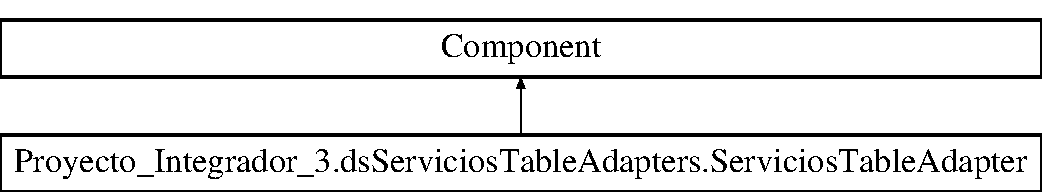
\includegraphics[height=2.000000cm]{d4/d3f/class_proyecto___integrador__3_1_1ds_servicios_table_adapters_1_1_servicios_table_adapter}
\end{center}
\end{figure}
\subsection*{Métodos públicos}
\begin{DoxyCompactItemize}
\item 
\hyperlink{class_proyecto___integrador__3_1_1ds_servicios_table_adapters_1_1_servicios_table_adapter_a16021c2eb24e9ee91eafb521a4d320b4}{Servicios\-Table\-Adapter} ()
\item 
virtual int \hyperlink{class_proyecto___integrador__3_1_1ds_servicios_table_adapters_1_1_servicios_table_adapter_ad0a281269dec2ad3d264f15b83b4fedf}{Fill} (\hyperlink{class_proyecto___integrador__3_1_1ds_servicios_1_1_servicios_data_table}{ds\-Servicios.\-Servicios\-Data\-Table} data\-Table)
\item 
virtual \\*
\hyperlink{class_proyecto___integrador__3_1_1ds_servicios_1_1_servicios_data_table}{ds\-Servicios.\-Servicios\-Data\-Table} \hyperlink{class_proyecto___integrador__3_1_1ds_servicios_table_adapters_1_1_servicios_table_adapter_a094ae05881b4c854d8eded668faae6c3}{Get\-Data} ()
\item 
virtual int \hyperlink{class_proyecto___integrador__3_1_1ds_servicios_table_adapters_1_1_servicios_table_adapter_aeef3160a3e0bdc86f499f0f9ad7221fd}{Update} (\hyperlink{class_proyecto___integrador__3_1_1ds_servicios_1_1_servicios_data_table}{ds\-Servicios.\-Servicios\-Data\-Table} data\-Table)
\item 
virtual int \hyperlink{class_proyecto___integrador__3_1_1ds_servicios_table_adapters_1_1_servicios_table_adapter_a3492851ad51e84e611ed56f599c8ed96}{Update} (\hyperlink{class_proyecto___integrador__3_1_1ds_servicios}{ds\-Servicios} data\-Set)
\item 
virtual int \hyperlink{class_proyecto___integrador__3_1_1ds_servicios_table_adapters_1_1_servicios_table_adapter_a029fffb4deea6ce4379d7858bc1a707c}{Update} (global\-::\-System.\-Data.\-Data\-Row data\-Row)
\item 
virtual int \hyperlink{class_proyecto___integrador__3_1_1ds_servicios_table_adapters_1_1_servicios_table_adapter_a4f3888665a7a03b764670069a0e923dd}{Update} (global\-::\-System.\-Data.\-Data\-Row\mbox{[}$\,$\mbox{]} data\-Rows)
\item 
virtual int \hyperlink{class_proyecto___integrador__3_1_1ds_servicios_table_adapters_1_1_servicios_table_adapter_ade09fa224ce227b1bd8132d103abb9bd}{Delete} (int Original\-\_\-id)
\item 
virtual int \hyperlink{class_proyecto___integrador__3_1_1ds_servicios_table_adapters_1_1_servicios_table_adapter_a8fdcc35bf82db2d196e665f73000ac0c}{Insert} (string tipo\-Usuario, System.\-Guid unidad, System.\-Guid usuario, System.\-Date\-Time fecha)
\item 
virtual int \hyperlink{class_proyecto___integrador__3_1_1ds_servicios_table_adapters_1_1_servicios_table_adapter_a5024e7973f369f5c0e4a3478f2660a75}{Update} (string tipo\-Usuario, System.\-Guid unidad, System.\-Guid usuario, System.\-Date\-Time fecha, int Original\-\_\-id)
\end{DoxyCompactItemize}
\subsection*{Propiedades}
\begin{DoxyCompactItemize}
\item 
global\-::\-System.\-Data.\-Sql\-Server\-Ce.\-Sql\-Ce\-Data\-Adapter \hyperlink{class_proyecto___integrador__3_1_1ds_servicios_table_adapters_1_1_servicios_table_adapter_a6e2d84a1b2c925ab5f078c403b1e3ecf}{Adapter}\hspace{0.3cm}{\ttfamily  \mbox{[}get\mbox{]}}
\item 
global\-::\-System.\-Data.\-Sql\-Server\-Ce.\-Sql\-Ce\-Connection \hyperlink{class_proyecto___integrador__3_1_1ds_servicios_table_adapters_1_1_servicios_table_adapter_afdc3759c0f8fd84ed6ae2943ee4855f5}{Connection}\hspace{0.3cm}{\ttfamily  \mbox{[}get, set\mbox{]}}
\item 
global\-::\-System.\-Data.\-Sql\-Server\-Ce.\-Sql\-Ce\-Transaction \hyperlink{class_proyecto___integrador__3_1_1ds_servicios_table_adapters_1_1_servicios_table_adapter_a3e7fe5479416cffb20c9576cdefb7e8e}{Transaction}\hspace{0.3cm}{\ttfamily  \mbox{[}get, set\mbox{]}}
\item 
global\-::\-System.\-Data.\-Sql\-Server\-Ce.\-Sql\-Ce\-Command\mbox{[}$\,$\mbox{]} \hyperlink{class_proyecto___integrador__3_1_1ds_servicios_table_adapters_1_1_servicios_table_adapter_ad42d3cd780a8573cb22d9a8a3c251cbc}{Command\-Collection}\hspace{0.3cm}{\ttfamily  \mbox{[}get\mbox{]}}
\item 
bool \hyperlink{class_proyecto___integrador__3_1_1ds_servicios_table_adapters_1_1_servicios_table_adapter_a10403cf7d526506e7a350a7ba70cc6ec}{Clear\-Before\-Fill}\hspace{0.3cm}{\ttfamily  \mbox{[}get, set\mbox{]}}
\end{DoxyCompactItemize}
\subsection*{Métodos privados}
\begin{DoxyCompactItemize}
\item 
void \hyperlink{class_proyecto___integrador__3_1_1ds_servicios_table_adapters_1_1_servicios_table_adapter_a4faac695dc160139a491938577b85da5}{Init\-Adapter} ()
\item 
void \hyperlink{class_proyecto___integrador__3_1_1ds_servicios_table_adapters_1_1_servicios_table_adapter_aba8164625c74a38ddd37f0558d58a78a}{Init\-Connection} ()
\item 
void \hyperlink{class_proyecto___integrador__3_1_1ds_servicios_table_adapters_1_1_servicios_table_adapter_a780a31923b2bcea2f1c260e08fb43064}{Init\-Command\-Collection} ()
\end{DoxyCompactItemize}
\subsection*{Atributos privados}
\begin{DoxyCompactItemize}
\item 
global\-::\-System.\-Data.\-Sql\-Server\-Ce.\-Sql\-Ce\-Data\-Adapter \hyperlink{class_proyecto___integrador__3_1_1ds_servicios_table_adapters_1_1_servicios_table_adapter_adef36d1c06bafba740cd2cb94515689b}{\-\_\-adapter}
\item 
global\-::\-System.\-Data.\-Sql\-Server\-Ce.\-Sql\-Ce\-Connection \hyperlink{class_proyecto___integrador__3_1_1ds_servicios_table_adapters_1_1_servicios_table_adapter_a61b17efa7b400219260090a16bfccff3}{\-\_\-connection}
\item 
global\-::\-System.\-Data.\-Sql\-Server\-Ce.\-Sql\-Ce\-Transaction \hyperlink{class_proyecto___integrador__3_1_1ds_servicios_table_adapters_1_1_servicios_table_adapter_ab5265bf458c29343cad2cc1c7f49da90}{\-\_\-transaction}
\item 
global\-::\-System.\-Data.\-Sql\-Server\-Ce.\-Sql\-Ce\-Command\mbox{[}$\,$\mbox{]} \hyperlink{class_proyecto___integrador__3_1_1ds_servicios_table_adapters_1_1_servicios_table_adapter_a1dce748dfee4379f6fb18ac2d87c3e5b}{\-\_\-command\-Collection}
\item 
bool \hyperlink{class_proyecto___integrador__3_1_1ds_servicios_table_adapters_1_1_servicios_table_adapter_af7f5af5748748a7cb81b440aab054f0e}{\-\_\-clear\-Before\-Fill}
\end{DoxyCompactItemize}


\subsection{Descripción detallada}
Represents the connection and commands used to retrieve and save data. 

/summary$>$ 

Definición en la línea 715 del archivo ds\-Servicios.\-Designer.\-cs.



\subsection{Documentación del constructor y destructor}
\hypertarget{class_proyecto___integrador__3_1_1ds_servicios_table_adapters_1_1_servicios_table_adapter_a16021c2eb24e9ee91eafb521a4d320b4}{\index{Proyecto\-\_\-\-Integrador\-\_\-3\-::ds\-Servicios\-Table\-Adapters\-::\-Servicios\-Table\-Adapter@{Proyecto\-\_\-\-Integrador\-\_\-3\-::ds\-Servicios\-Table\-Adapters\-::\-Servicios\-Table\-Adapter}!Servicios\-Table\-Adapter@{Servicios\-Table\-Adapter}}
\index{Servicios\-Table\-Adapter@{Servicios\-Table\-Adapter}!Proyecto_Integrador_3::dsServiciosTableAdapters::ServiciosTableAdapter@{Proyecto\-\_\-\-Integrador\-\_\-3\-::ds\-Servicios\-Table\-Adapters\-::\-Servicios\-Table\-Adapter}}
\subsubsection[{Servicios\-Table\-Adapter}]{\setlength{\rightskip}{0pt plus 5cm}Proyecto\-\_\-\-Integrador\-\_\-3.\-ds\-Servicios\-Table\-Adapters.\-Servicios\-Table\-Adapter.\-Servicios\-Table\-Adapter (
\begin{DoxyParamCaption}
{}
\end{DoxyParamCaption}
)\hspace{0.3cm}{\ttfamily [inline]}}}\label{class_proyecto___integrador__3_1_1ds_servicios_table_adapters_1_1_servicios_table_adapter_a16021c2eb24e9ee91eafb521a4d320b4}


Definición en la línea 729 del archivo ds\-Servicios.\-Designer.\-cs.


\begin{DoxyCode}
729                                        \{
730             this.\hyperlink{class_proyecto___integrador__3_1_1ds_servicios_table_adapters_1_1_servicios_table_adapter_a10403cf7d526506e7a350a7ba70cc6ec}{ClearBeforeFill} = \textcolor{keyword}{true};
731         \}
\end{DoxyCode}


\subsection{Documentación de las funciones miembro}
\hypertarget{class_proyecto___integrador__3_1_1ds_servicios_table_adapters_1_1_servicios_table_adapter_ade09fa224ce227b1bd8132d103abb9bd}{\index{Proyecto\-\_\-\-Integrador\-\_\-3\-::ds\-Servicios\-Table\-Adapters\-::\-Servicios\-Table\-Adapter@{Proyecto\-\_\-\-Integrador\-\_\-3\-::ds\-Servicios\-Table\-Adapters\-::\-Servicios\-Table\-Adapter}!Delete@{Delete}}
\index{Delete@{Delete}!Proyecto_Integrador_3::dsServiciosTableAdapters::ServiciosTableAdapter@{Proyecto\-\_\-\-Integrador\-\_\-3\-::ds\-Servicios\-Table\-Adapters\-::\-Servicios\-Table\-Adapter}}
\subsubsection[{Delete}]{\setlength{\rightskip}{0pt plus 5cm}virtual int Proyecto\-\_\-\-Integrador\-\_\-3.\-ds\-Servicios\-Table\-Adapters.\-Servicios\-Table\-Adapter.\-Delete (
\begin{DoxyParamCaption}
\item[{int}]{Original\-\_\-id}
\end{DoxyParamCaption}
)\hspace{0.3cm}{\ttfamily [inline]}, {\ttfamily [virtual]}}}\label{class_proyecto___integrador__3_1_1ds_servicios_table_adapters_1_1_servicios_table_adapter_ade09fa224ce227b1bd8132d103abb9bd}


Definición en la línea 933 del archivo ds\-Servicios.\-Designer.\-cs.


\begin{DoxyCode}
933                                                    \{
934             this.\hyperlink{class_proyecto___integrador__3_1_1ds_servicios_table_adapters_1_1_servicios_table_adapter_a6e2d84a1b2c925ab5f078c403b1e3ecf}{Adapter}.DeleteCommand.Parameters[0].Value = ((int)(Original\_id));
935             global::System.Data.ConnectionState previousConnectionState = this.
      \hyperlink{class_proyecto___integrador__3_1_1ds_servicios_table_adapters_1_1_servicios_table_adapter_a6e2d84a1b2c925ab5f078c403b1e3ecf}{Adapter}.DeleteCommand.Connection.State;
936             \textcolor{keywordflow}{if} (((this.\hyperlink{class_proyecto___integrador__3_1_1ds_servicios_table_adapters_1_1_servicios_table_adapter_a6e2d84a1b2c925ab5f078c403b1e3ecf}{Adapter}.DeleteCommand.Connection.State & global::System.Data.ConnectionState.
      Open) 
937                         != global::System.Data.ConnectionState.Open)) \{
938                 this.\hyperlink{class_proyecto___integrador__3_1_1ds_servicios_table_adapters_1_1_servicios_table_adapter_a6e2d84a1b2c925ab5f078c403b1e3ecf}{Adapter}.DeleteCommand.Connection.Open();
939             \}
940             \textcolor{keywordflow}{try} \{
941                 \textcolor{keywordtype}{int} returnValue = this.\hyperlink{class_proyecto___integrador__3_1_1ds_servicios_table_adapters_1_1_servicios_table_adapter_a6e2d84a1b2c925ab5f078c403b1e3ecf}{Adapter}.DeleteCommand.ExecuteNonQuery();
942                 \textcolor{keywordflow}{return} returnValue;
943             \}
944             \textcolor{keywordflow}{finally} \{
945                 \textcolor{keywordflow}{if} ((previousConnectionState == global::System.Data.ConnectionState.Closed)) \{
946                     this.\hyperlink{class_proyecto___integrador__3_1_1ds_servicios_table_adapters_1_1_servicios_table_adapter_a6e2d84a1b2c925ab5f078c403b1e3ecf}{Adapter}.DeleteCommand.Connection.Close();
947                 \}
948             \}
949         \}
\end{DoxyCode}
\hypertarget{class_proyecto___integrador__3_1_1ds_servicios_table_adapters_1_1_servicios_table_adapter_ad0a281269dec2ad3d264f15b83b4fedf}{\index{Proyecto\-\_\-\-Integrador\-\_\-3\-::ds\-Servicios\-Table\-Adapters\-::\-Servicios\-Table\-Adapter@{Proyecto\-\_\-\-Integrador\-\_\-3\-::ds\-Servicios\-Table\-Adapters\-::\-Servicios\-Table\-Adapter}!Fill@{Fill}}
\index{Fill@{Fill}!Proyecto_Integrador_3::dsServiciosTableAdapters::ServiciosTableAdapter@{Proyecto\-\_\-\-Integrador\-\_\-3\-::ds\-Servicios\-Table\-Adapters\-::\-Servicios\-Table\-Adapter}}
\subsubsection[{Fill}]{\setlength{\rightskip}{0pt plus 5cm}virtual int Proyecto\-\_\-\-Integrador\-\_\-3.\-ds\-Servicios\-Table\-Adapters.\-Servicios\-Table\-Adapter.\-Fill (
\begin{DoxyParamCaption}
\item[{{\bf ds\-Servicios.\-Servicios\-Data\-Table}}]{data\-Table}
\end{DoxyParamCaption}
)\hspace{0.3cm}{\ttfamily [inline]}, {\ttfamily [virtual]}}}\label{class_proyecto___integrador__3_1_1ds_servicios_table_adapters_1_1_servicios_table_adapter_ad0a281269dec2ad3d264f15b83b4fedf}


Definición en la línea 880 del archivo ds\-Servicios.\-Designer.\-cs.


\begin{DoxyCode}
880                                                                           \{
881             this.\hyperlink{class_proyecto___integrador__3_1_1ds_servicios_table_adapters_1_1_servicios_table_adapter_a6e2d84a1b2c925ab5f078c403b1e3ecf}{Adapter}.SelectCommand = this.\hyperlink{class_proyecto___integrador__3_1_1ds_servicios_table_adapters_1_1_servicios_table_adapter_ad42d3cd780a8573cb22d9a8a3c251cbc}{CommandCollection}[0];
882             \textcolor{keywordflow}{if} ((this.\hyperlink{class_proyecto___integrador__3_1_1ds_servicios_table_adapters_1_1_servicios_table_adapter_a10403cf7d526506e7a350a7ba70cc6ec}{ClearBeforeFill} == \textcolor{keyword}{true})) \{
883                 dataTable.Clear();
884             \}
885             \textcolor{keywordtype}{int} returnValue = this.\hyperlink{class_proyecto___integrador__3_1_1ds_servicios_table_adapters_1_1_servicios_table_adapter_a6e2d84a1b2c925ab5f078c403b1e3ecf}{Adapter}.Fill(dataTable);
886             \textcolor{keywordflow}{return} returnValue;
887         \}
\end{DoxyCode}
\hypertarget{class_proyecto___integrador__3_1_1ds_servicios_table_adapters_1_1_servicios_table_adapter_a094ae05881b4c854d8eded668faae6c3}{\index{Proyecto\-\_\-\-Integrador\-\_\-3\-::ds\-Servicios\-Table\-Adapters\-::\-Servicios\-Table\-Adapter@{Proyecto\-\_\-\-Integrador\-\_\-3\-::ds\-Servicios\-Table\-Adapters\-::\-Servicios\-Table\-Adapter}!Get\-Data@{Get\-Data}}
\index{Get\-Data@{Get\-Data}!Proyecto_Integrador_3::dsServiciosTableAdapters::ServiciosTableAdapter@{Proyecto\-\_\-\-Integrador\-\_\-3\-::ds\-Servicios\-Table\-Adapters\-::\-Servicios\-Table\-Adapter}}
\subsubsection[{Get\-Data}]{\setlength{\rightskip}{0pt plus 5cm}virtual {\bf ds\-Servicios.\-Servicios\-Data\-Table} Proyecto\-\_\-\-Integrador\-\_\-3.\-ds\-Servicios\-Table\-Adapters.\-Servicios\-Table\-Adapter.\-Get\-Data (
\begin{DoxyParamCaption}
{}
\end{DoxyParamCaption}
)\hspace{0.3cm}{\ttfamily [inline]}, {\ttfamily [virtual]}}}\label{class_proyecto___integrador__3_1_1ds_servicios_table_adapters_1_1_servicios_table_adapter_a094ae05881b4c854d8eded668faae6c3}


Definición en la línea 893 del archivo ds\-Servicios.\-Designer.\-cs.


\begin{DoxyCode}
893                                                                 \{
894             this.\hyperlink{class_proyecto___integrador__3_1_1ds_servicios_table_adapters_1_1_servicios_table_adapter_a6e2d84a1b2c925ab5f078c403b1e3ecf}{Adapter}.SelectCommand = this.\hyperlink{class_proyecto___integrador__3_1_1ds_servicios_table_adapters_1_1_servicios_table_adapter_ad42d3cd780a8573cb22d9a8a3c251cbc}{CommandCollection}[0];
895             dsServicios.ServiciosDataTable dataTable = \textcolor{keyword}{new} dsServicios.ServiciosDataTable();
896             this.\hyperlink{class_proyecto___integrador__3_1_1ds_servicios_table_adapters_1_1_servicios_table_adapter_a6e2d84a1b2c925ab5f078c403b1e3ecf}{Adapter}.Fill(dataTable);
897             \textcolor{keywordflow}{return} dataTable;
898         \}
\end{DoxyCode}
\hypertarget{class_proyecto___integrador__3_1_1ds_servicios_table_adapters_1_1_servicios_table_adapter_a4faac695dc160139a491938577b85da5}{\index{Proyecto\-\_\-\-Integrador\-\_\-3\-::ds\-Servicios\-Table\-Adapters\-::\-Servicios\-Table\-Adapter@{Proyecto\-\_\-\-Integrador\-\_\-3\-::ds\-Servicios\-Table\-Adapters\-::\-Servicios\-Table\-Adapter}!Init\-Adapter@{Init\-Adapter}}
\index{Init\-Adapter@{Init\-Adapter}!Proyecto_Integrador_3::dsServiciosTableAdapters::ServiciosTableAdapter@{Proyecto\-\_\-\-Integrador\-\_\-3\-::ds\-Servicios\-Table\-Adapters\-::\-Servicios\-Table\-Adapter}}
\subsubsection[{Init\-Adapter}]{\setlength{\rightskip}{0pt plus 5cm}void Proyecto\-\_\-\-Integrador\-\_\-3.\-ds\-Servicios\-Table\-Adapters.\-Servicios\-Table\-Adapter.\-Init\-Adapter (
\begin{DoxyParamCaption}
{}
\end{DoxyParamCaption}
)\hspace{0.3cm}{\ttfamily [inline]}, {\ttfamily [private]}}}\label{class_proyecto___integrador__3_1_1ds_servicios_table_adapters_1_1_servicios_table_adapter_a4faac695dc160139a491938577b85da5}


Definición en la línea 822 del archivo ds\-Servicios.\-Designer.\-cs.


\begin{DoxyCode}
822                                    \{
823             this.\hyperlink{class_proyecto___integrador__3_1_1ds_servicios_table_adapters_1_1_servicios_table_adapter_adef36d1c06bafba740cd2cb94515689b}{\_adapter} = \textcolor{keyword}{new} global::System.Data.SqlServerCe.SqlCeDataAdapter();
824             global::System.Data.Common.DataTableMapping tableMapping = \textcolor{keyword}{new} global::System.Data.Common.
      DataTableMapping();
825             tableMapping.SourceTable = \textcolor{stringliteral}{"Table"};
826             tableMapping.DataSetTable = \textcolor{stringliteral}{"Servicios"};
827             tableMapping.ColumnMappings.Add(\textcolor{stringliteral}{"id"}, \textcolor{stringliteral}{"id"});
828             tableMapping.ColumnMappings.Add(\textcolor{stringliteral}{"tipoUsuario"}, \textcolor{stringliteral}{"tipoUsuario"});
829             tableMapping.ColumnMappings.Add(\textcolor{stringliteral}{"unidad"}, \textcolor{stringliteral}{"unidad"});
830             tableMapping.ColumnMappings.Add(\textcolor{stringliteral}{"usuario"}, \textcolor{stringliteral}{"usuario"});
831             tableMapping.ColumnMappings.Add(\textcolor{stringliteral}{"fecha"}, \textcolor{stringliteral}{"fecha"});
832             this.\hyperlink{class_proyecto___integrador__3_1_1ds_servicios_table_adapters_1_1_servicios_table_adapter_adef36d1c06bafba740cd2cb94515689b}{\_adapter}.TableMappings.Add(tableMapping);
833             this.\hyperlink{class_proyecto___integrador__3_1_1ds_servicios_table_adapters_1_1_servicios_table_adapter_adef36d1c06bafba740cd2cb94515689b}{\_adapter}.DeleteCommand = \textcolor{keyword}{new} global::System.Data.SqlServerCe.SqlCeCommand();
834             this.\hyperlink{class_proyecto___integrador__3_1_1ds_servicios_table_adapters_1_1_servicios_table_adapter_adef36d1c06bafba740cd2cb94515689b}{\_adapter}.DeleteCommand.Connection = this.\hyperlink{class_proyecto___integrador__3_1_1ds_servicios_table_adapters_1_1_servicios_table_adapter_afdc3759c0f8fd84ed6ae2943ee4855f5}{Connection};
835             this.\hyperlink{class_proyecto___integrador__3_1_1ds_servicios_table_adapters_1_1_servicios_table_adapter_adef36d1c06bafba740cd2cb94515689b}{\_adapter}.DeleteCommand.CommandText = \textcolor{stringliteral}{"DELETE FROM [Servicios] WHERE (([id] =
       @Original\_id))"};
836             this.\hyperlink{class_proyecto___integrador__3_1_1ds_servicios_table_adapters_1_1_servicios_table_adapter_adef36d1c06bafba740cd2cb94515689b}{\_adapter}.DeleteCommand.CommandType = global::System.Data.CommandType.Text;
837             this.\hyperlink{class_proyecto___integrador__3_1_1ds_servicios_table_adapters_1_1_servicios_table_adapter_adef36d1c06bafba740cd2cb94515689b}{\_adapter}.DeleteCommand.Parameters.Add(\textcolor{keyword}{new} global::System.Data.SqlServerCe.
      SqlCeParameter(\textcolor{stringliteral}{"@Original\_id"}, global::System.Data.SqlDbType.Int, 0, global::System.Data.ParameterDirection.Input, \textcolor{keyword}{
      true}, 0, 0, \textcolor{stringliteral}{"id"}, global::System.Data.DataRowVersion.Original, null));
838             this.\hyperlink{class_proyecto___integrador__3_1_1ds_servicios_table_adapters_1_1_servicios_table_adapter_adef36d1c06bafba740cd2cb94515689b}{\_adapter}.InsertCommand = \textcolor{keyword}{new} global::System.Data.SqlServerCe.SqlCeCommand();
839             this.\hyperlink{class_proyecto___integrador__3_1_1ds_servicios_table_adapters_1_1_servicios_table_adapter_adef36d1c06bafba740cd2cb94515689b}{\_adapter}.InsertCommand.Connection = this.\hyperlink{class_proyecto___integrador__3_1_1ds_servicios_table_adapters_1_1_servicios_table_adapter_afdc3759c0f8fd84ed6ae2943ee4855f5}{Connection};
840             this.\hyperlink{class_proyecto___integrador__3_1_1ds_servicios_table_adapters_1_1_servicios_table_adapter_adef36d1c06bafba740cd2cb94515689b}{\_adapter}.InsertCommand.CommandText = \textcolor{stringliteral}{"INSERT INTO [Servicios] ([tipoUsuario],
       [unidad], [usuario], [fecha]) VALUES (@ti"} +
841                 \textcolor{stringliteral}{"poUsuario, @unidad, @usuario, @fecha)"};
842             this.\hyperlink{class_proyecto___integrador__3_1_1ds_servicios_table_adapters_1_1_servicios_table_adapter_adef36d1c06bafba740cd2cb94515689b}{\_adapter}.InsertCommand.CommandType = global::System.Data.CommandType.Text;
843             this.\hyperlink{class_proyecto___integrador__3_1_1ds_servicios_table_adapters_1_1_servicios_table_adapter_adef36d1c06bafba740cd2cb94515689b}{\_adapter}.InsertCommand.Parameters.Add(\textcolor{keyword}{new} global::System.Data.SqlServerCe.
      SqlCeParameter(\textcolor{stringliteral}{"@tipoUsuario"}, global::System.Data.SqlDbType.NVarChar, 0, global::System.Data.ParameterDirection.
      Input, \textcolor{keyword}{true}, 0, 0, \textcolor{stringliteral}{"tipoUsuario"}, global::System.Data.DataRowVersion.Current, null));
844             this.\hyperlink{class_proyecto___integrador__3_1_1ds_servicios_table_adapters_1_1_servicios_table_adapter_adef36d1c06bafba740cd2cb94515689b}{\_adapter}.InsertCommand.Parameters.Add(\textcolor{keyword}{new} global::System.Data.SqlServerCe.
      SqlCeParameter(\textcolor{stringliteral}{"@unidad"}, global::System.Data.SqlDbType.UniqueIdentifier, 0, global::System.Data.ParameterDirection.
      Input, \textcolor{keyword}{true}, 0, 0, \textcolor{stringliteral}{"unidad"}, global::System.Data.DataRowVersion.Current, null));
845             this.\hyperlink{class_proyecto___integrador__3_1_1ds_servicios_table_adapters_1_1_servicios_table_adapter_adef36d1c06bafba740cd2cb94515689b}{\_adapter}.InsertCommand.Parameters.Add(\textcolor{keyword}{new} global::System.Data.SqlServerCe.
      SqlCeParameter(\textcolor{stringliteral}{"@usuario"}, global::System.Data.SqlDbType.UniqueIdentifier, 0, global::System.Data.ParameterDirection
      .Input, \textcolor{keyword}{true}, 0, 0, \textcolor{stringliteral}{"usuario"}, global::System.Data.DataRowVersion.Current, null));
846             this.\hyperlink{class_proyecto___integrador__3_1_1ds_servicios_table_adapters_1_1_servicios_table_adapter_adef36d1c06bafba740cd2cb94515689b}{\_adapter}.InsertCommand.Parameters.Add(\textcolor{keyword}{new} global::System.Data.SqlServerCe.
      SqlCeParameter(\textcolor{stringliteral}{"@fecha"}, global::System.Data.SqlDbType.DateTime, 0, global::System.Data.ParameterDirection.Input, \textcolor{keyword}{
      true}, 0, 0, \textcolor{stringliteral}{"fecha"}, global::System.Data.DataRowVersion.Current, null));
847             this.\hyperlink{class_proyecto___integrador__3_1_1ds_servicios_table_adapters_1_1_servicios_table_adapter_adef36d1c06bafba740cd2cb94515689b}{\_adapter}.UpdateCommand = \textcolor{keyword}{new} global::System.Data.SqlServerCe.SqlCeCommand();
848             this.\hyperlink{class_proyecto___integrador__3_1_1ds_servicios_table_adapters_1_1_servicios_table_adapter_adef36d1c06bafba740cd2cb94515689b}{\_adapter}.UpdateCommand.Connection = this.\hyperlink{class_proyecto___integrador__3_1_1ds_servicios_table_adapters_1_1_servicios_table_adapter_afdc3759c0f8fd84ed6ae2943ee4855f5}{Connection};
849             this.\hyperlink{class_proyecto___integrador__3_1_1ds_servicios_table_adapters_1_1_servicios_table_adapter_adef36d1c06bafba740cd2cb94515689b}{\_adapter}.UpdateCommand.CommandText = \textcolor{stringliteral}{"UPDATE [Servicios] SET [tipoUsuario] =
       @tipoUsuario, [unidad] = @unidad, [usuario"} +
850                 \textcolor{stringliteral}{"] = @usuario, [fecha] = @fecha WHERE (([id] = @Original\_id))"};
851             this.\hyperlink{class_proyecto___integrador__3_1_1ds_servicios_table_adapters_1_1_servicios_table_adapter_adef36d1c06bafba740cd2cb94515689b}{\_adapter}.UpdateCommand.CommandType = global::System.Data.CommandType.Text;
852             this.\hyperlink{class_proyecto___integrador__3_1_1ds_servicios_table_adapters_1_1_servicios_table_adapter_adef36d1c06bafba740cd2cb94515689b}{\_adapter}.UpdateCommand.Parameters.Add(\textcolor{keyword}{new} global::System.Data.SqlServerCe.
      SqlCeParameter(\textcolor{stringliteral}{"@tipoUsuario"}, global::System.Data.SqlDbType.NVarChar, 0, global::System.Data.ParameterDirection.
      Input, \textcolor{keyword}{true}, 0, 0, \textcolor{stringliteral}{"tipoUsuario"}, global::System.Data.DataRowVersion.Current, null));
853             this.\hyperlink{class_proyecto___integrador__3_1_1ds_servicios_table_adapters_1_1_servicios_table_adapter_adef36d1c06bafba740cd2cb94515689b}{\_adapter}.UpdateCommand.Parameters.Add(\textcolor{keyword}{new} global::System.Data.SqlServerCe.
      SqlCeParameter(\textcolor{stringliteral}{"@unidad"}, global::System.Data.SqlDbType.UniqueIdentifier, 0, global::System.Data.ParameterDirection.
      Input, \textcolor{keyword}{true}, 0, 0, \textcolor{stringliteral}{"unidad"}, global::System.Data.DataRowVersion.Current, null));
854             this.\hyperlink{class_proyecto___integrador__3_1_1ds_servicios_table_adapters_1_1_servicios_table_adapter_adef36d1c06bafba740cd2cb94515689b}{\_adapter}.UpdateCommand.Parameters.Add(\textcolor{keyword}{new} global::System.Data.SqlServerCe.
      SqlCeParameter(\textcolor{stringliteral}{"@usuario"}, global::System.Data.SqlDbType.UniqueIdentifier, 0, global::System.Data.ParameterDirection
      .Input, \textcolor{keyword}{true}, 0, 0, \textcolor{stringliteral}{"usuario"}, global::System.Data.DataRowVersion.Current, null));
855             this.\hyperlink{class_proyecto___integrador__3_1_1ds_servicios_table_adapters_1_1_servicios_table_adapter_adef36d1c06bafba740cd2cb94515689b}{\_adapter}.UpdateCommand.Parameters.Add(\textcolor{keyword}{new} global::System.Data.SqlServerCe.
      SqlCeParameter(\textcolor{stringliteral}{"@fecha"}, global::System.Data.SqlDbType.DateTime, 0, global::System.Data.ParameterDirection.Input, \textcolor{keyword}{
      true}, 0, 0, \textcolor{stringliteral}{"fecha"}, global::System.Data.DataRowVersion.Current, null));
856             this.\hyperlink{class_proyecto___integrador__3_1_1ds_servicios_table_adapters_1_1_servicios_table_adapter_adef36d1c06bafba740cd2cb94515689b}{\_adapter}.UpdateCommand.Parameters.Add(\textcolor{keyword}{new} global::System.Data.SqlServerCe.
      SqlCeParameter(\textcolor{stringliteral}{"@Original\_id"}, global::System.Data.SqlDbType.Int, 0, global::System.Data.ParameterDirection.Input, \textcolor{keyword}{
      true}, 0, 0, \textcolor{stringliteral}{"id"}, global::System.Data.DataRowVersion.Original, null));
857         \}
\end{DoxyCode}
\hypertarget{class_proyecto___integrador__3_1_1ds_servicios_table_adapters_1_1_servicios_table_adapter_a780a31923b2bcea2f1c260e08fb43064}{\index{Proyecto\-\_\-\-Integrador\-\_\-3\-::ds\-Servicios\-Table\-Adapters\-::\-Servicios\-Table\-Adapter@{Proyecto\-\_\-\-Integrador\-\_\-3\-::ds\-Servicios\-Table\-Adapters\-::\-Servicios\-Table\-Adapter}!Init\-Command\-Collection@{Init\-Command\-Collection}}
\index{Init\-Command\-Collection@{Init\-Command\-Collection}!Proyecto_Integrador_3::dsServiciosTableAdapters::ServiciosTableAdapter@{Proyecto\-\_\-\-Integrador\-\_\-3\-::ds\-Servicios\-Table\-Adapters\-::\-Servicios\-Table\-Adapter}}
\subsubsection[{Init\-Command\-Collection}]{\setlength{\rightskip}{0pt plus 5cm}void Proyecto\-\_\-\-Integrador\-\_\-3.\-ds\-Servicios\-Table\-Adapters.\-Servicios\-Table\-Adapter.\-Init\-Command\-Collection (
\begin{DoxyParamCaption}
{}
\end{DoxyParamCaption}
)\hspace{0.3cm}{\ttfamily [inline]}, {\ttfamily [private]}}}\label{class_proyecto___integrador__3_1_1ds_servicios_table_adapters_1_1_servicios_table_adapter_a780a31923b2bcea2f1c260e08fb43064}


Definición en la línea 868 del archivo ds\-Servicios.\-Designer.\-cs.


\begin{DoxyCode}
868                                              \{
869             this.\hyperlink{class_proyecto___integrador__3_1_1ds_servicios_table_adapters_1_1_servicios_table_adapter_a1dce748dfee4379f6fb18ac2d87c3e5b}{\_commandCollection} = \textcolor{keyword}{new} global::System.Data.SqlServerCe.SqlCeCommand[1]
      ;
870             this.\hyperlink{class_proyecto___integrador__3_1_1ds_servicios_table_adapters_1_1_servicios_table_adapter_a1dce748dfee4379f6fb18ac2d87c3e5b}{\_commandCollection}[0] = \textcolor{keyword}{new} global::System.Data.SqlServerCe.SqlCeCommand
      ();
871             this.\hyperlink{class_proyecto___integrador__3_1_1ds_servicios_table_adapters_1_1_servicios_table_adapter_a1dce748dfee4379f6fb18ac2d87c3e5b}{\_commandCollection}[0].Connection = this.
      \hyperlink{class_proyecto___integrador__3_1_1ds_servicios_table_adapters_1_1_servicios_table_adapter_afdc3759c0f8fd84ed6ae2943ee4855f5}{Connection};
872             this.\hyperlink{class_proyecto___integrador__3_1_1ds_servicios_table_adapters_1_1_servicios_table_adapter_a1dce748dfee4379f6fb18ac2d87c3e5b}{\_commandCollection}[0].CommandText = \textcolor{stringliteral}{"SELECT Servicios.*\(\backslash\)r\(\backslash\)nFROM    
       Servicios"};
873             this.\hyperlink{class_proyecto___integrador__3_1_1ds_servicios_table_adapters_1_1_servicios_table_adapter_a1dce748dfee4379f6fb18ac2d87c3e5b}{\_commandCollection}[0].CommandType = global::System.Data.CommandType.Text
      ;
874         \}
\end{DoxyCode}
\hypertarget{class_proyecto___integrador__3_1_1ds_servicios_table_adapters_1_1_servicios_table_adapter_aba8164625c74a38ddd37f0558d58a78a}{\index{Proyecto\-\_\-\-Integrador\-\_\-3\-::ds\-Servicios\-Table\-Adapters\-::\-Servicios\-Table\-Adapter@{Proyecto\-\_\-\-Integrador\-\_\-3\-::ds\-Servicios\-Table\-Adapters\-::\-Servicios\-Table\-Adapter}!Init\-Connection@{Init\-Connection}}
\index{Init\-Connection@{Init\-Connection}!Proyecto_Integrador_3::dsServiciosTableAdapters::ServiciosTableAdapter@{Proyecto\-\_\-\-Integrador\-\_\-3\-::ds\-Servicios\-Table\-Adapters\-::\-Servicios\-Table\-Adapter}}
\subsubsection[{Init\-Connection}]{\setlength{\rightskip}{0pt plus 5cm}void Proyecto\-\_\-\-Integrador\-\_\-3.\-ds\-Servicios\-Table\-Adapters.\-Servicios\-Table\-Adapter.\-Init\-Connection (
\begin{DoxyParamCaption}
{}
\end{DoxyParamCaption}
)\hspace{0.3cm}{\ttfamily [inline]}, {\ttfamily [private]}}}\label{class_proyecto___integrador__3_1_1ds_servicios_table_adapters_1_1_servicios_table_adapter_aba8164625c74a38ddd37f0558d58a78a}


Definición en la línea 861 del archivo ds\-Servicios.\-Designer.\-cs.


\begin{DoxyCode}
861                                       \{
862             this.\hyperlink{class_proyecto___integrador__3_1_1ds_servicios_table_adapters_1_1_servicios_table_adapter_a61b17efa7b400219260090a16bfccff3}{\_connection} = \textcolor{keyword}{new} global::System.Data.SqlServerCe.SqlCeConnection();
863             this.\hyperlink{class_proyecto___integrador__3_1_1ds_servicios_table_adapters_1_1_servicios_table_adapter_a61b17efa7b400219260090a16bfccff3}{\_connection}.ConnectionString = global::Proyecto\_Integrador\_3.Properties.
      Settings.Default.ProyectoIntegradorConnectionString;
864         \}
\end{DoxyCode}
\hypertarget{class_proyecto___integrador__3_1_1ds_servicios_table_adapters_1_1_servicios_table_adapter_a8fdcc35bf82db2d196e665f73000ac0c}{\index{Proyecto\-\_\-\-Integrador\-\_\-3\-::ds\-Servicios\-Table\-Adapters\-::\-Servicios\-Table\-Adapter@{Proyecto\-\_\-\-Integrador\-\_\-3\-::ds\-Servicios\-Table\-Adapters\-::\-Servicios\-Table\-Adapter}!Insert@{Insert}}
\index{Insert@{Insert}!Proyecto_Integrador_3::dsServiciosTableAdapters::ServiciosTableAdapter@{Proyecto\-\_\-\-Integrador\-\_\-3\-::ds\-Servicios\-Table\-Adapters\-::\-Servicios\-Table\-Adapter}}
\subsubsection[{Insert}]{\setlength{\rightskip}{0pt plus 5cm}virtual int Proyecto\-\_\-\-Integrador\-\_\-3.\-ds\-Servicios\-Table\-Adapters.\-Servicios\-Table\-Adapter.\-Insert (
\begin{DoxyParamCaption}
\item[{string}]{tipo\-Usuario, }
\item[{System.\-Guid}]{unidad, }
\item[{System.\-Guid}]{usuario, }
\item[{System.\-Date\-Time}]{fecha}
\end{DoxyParamCaption}
)\hspace{0.3cm}{\ttfamily [inline]}, {\ttfamily [virtual]}}}\label{class_proyecto___integrador__3_1_1ds_servicios_table_adapters_1_1_servicios_table_adapter_a8fdcc35bf82db2d196e665f73000ac0c}


Definición en la línea 955 del archivo ds\-Servicios.\-Designer.\-cs.


\begin{DoxyCode}
955                                                                                                            
                 \{
956             \textcolor{keywordflow}{if} ((tipoUsuario == null)) \{
957                 \textcolor{keywordflow}{throw} \textcolor{keyword}{new} global::System.ArgumentNullException(\textcolor{stringliteral}{"tipoUsuario"});
958             \}
959             \textcolor{keywordflow}{else} \{
960                 this.\hyperlink{class_proyecto___integrador__3_1_1ds_servicios_table_adapters_1_1_servicios_table_adapter_a6e2d84a1b2c925ab5f078c403b1e3ecf}{Adapter}.InsertCommand.Parameters[0].Value = ((string)(tipoUsuario));
961             \}
962             this.\hyperlink{class_proyecto___integrador__3_1_1ds_servicios_table_adapters_1_1_servicios_table_adapter_a6e2d84a1b2c925ab5f078c403b1e3ecf}{Adapter}.InsertCommand.Parameters[1].Value = ((System.Guid)(unidad));
963             this.\hyperlink{class_proyecto___integrador__3_1_1ds_servicios_table_adapters_1_1_servicios_table_adapter_a6e2d84a1b2c925ab5f078c403b1e3ecf}{Adapter}.InsertCommand.Parameters[2].Value = ((System.Guid)(usuario));
964             this.\hyperlink{class_proyecto___integrador__3_1_1ds_servicios_table_adapters_1_1_servicios_table_adapter_a6e2d84a1b2c925ab5f078c403b1e3ecf}{Adapter}.InsertCommand.Parameters[3].Value = ((System.DateTime)(fecha));
965             global::System.Data.ConnectionState previousConnectionState = this.
      \hyperlink{class_proyecto___integrador__3_1_1ds_servicios_table_adapters_1_1_servicios_table_adapter_a6e2d84a1b2c925ab5f078c403b1e3ecf}{Adapter}.InsertCommand.Connection.State;
966             \textcolor{keywordflow}{if} (((this.\hyperlink{class_proyecto___integrador__3_1_1ds_servicios_table_adapters_1_1_servicios_table_adapter_a6e2d84a1b2c925ab5f078c403b1e3ecf}{Adapter}.InsertCommand.Connection.State & global::System.Data.ConnectionState.
      Open) 
967                         != global::System.Data.ConnectionState.Open)) \{
968                 this.\hyperlink{class_proyecto___integrador__3_1_1ds_servicios_table_adapters_1_1_servicios_table_adapter_a6e2d84a1b2c925ab5f078c403b1e3ecf}{Adapter}.InsertCommand.Connection.Open();
969             \}
970             \textcolor{keywordflow}{try} \{
971                 \textcolor{keywordtype}{int} returnValue = this.\hyperlink{class_proyecto___integrador__3_1_1ds_servicios_table_adapters_1_1_servicios_table_adapter_a6e2d84a1b2c925ab5f078c403b1e3ecf}{Adapter}.InsertCommand.ExecuteNonQuery();
972                 \textcolor{keywordflow}{return} returnValue;
973             \}
974             \textcolor{keywordflow}{finally} \{
975                 \textcolor{keywordflow}{if} ((previousConnectionState == global::System.Data.ConnectionState.Closed)) \{
976                     this.\hyperlink{class_proyecto___integrador__3_1_1ds_servicios_table_adapters_1_1_servicios_table_adapter_a6e2d84a1b2c925ab5f078c403b1e3ecf}{Adapter}.InsertCommand.Connection.Close();
977                 \}
978             \}
979         \}
\end{DoxyCode}
\hypertarget{class_proyecto___integrador__3_1_1ds_servicios_table_adapters_1_1_servicios_table_adapter_aeef3160a3e0bdc86f499f0f9ad7221fd}{\index{Proyecto\-\_\-\-Integrador\-\_\-3\-::ds\-Servicios\-Table\-Adapters\-::\-Servicios\-Table\-Adapter@{Proyecto\-\_\-\-Integrador\-\_\-3\-::ds\-Servicios\-Table\-Adapters\-::\-Servicios\-Table\-Adapter}!Update@{Update}}
\index{Update@{Update}!Proyecto_Integrador_3::dsServiciosTableAdapters::ServiciosTableAdapter@{Proyecto\-\_\-\-Integrador\-\_\-3\-::ds\-Servicios\-Table\-Adapters\-::\-Servicios\-Table\-Adapter}}
\subsubsection[{Update}]{\setlength{\rightskip}{0pt plus 5cm}virtual int Proyecto\-\_\-\-Integrador\-\_\-3.\-ds\-Servicios\-Table\-Adapters.\-Servicios\-Table\-Adapter.\-Update (
\begin{DoxyParamCaption}
\item[{{\bf ds\-Servicios.\-Servicios\-Data\-Table}}]{data\-Table}
\end{DoxyParamCaption}
)\hspace{0.3cm}{\ttfamily [inline]}, {\ttfamily [virtual]}}}\label{class_proyecto___integrador__3_1_1ds_servicios_table_adapters_1_1_servicios_table_adapter_aeef3160a3e0bdc86f499f0f9ad7221fd}


Definición en la línea 903 del archivo ds\-Servicios.\-Designer.\-cs.


\begin{DoxyCode}
903                                                                             \{
904             \textcolor{keywordflow}{return} this.\hyperlink{class_proyecto___integrador__3_1_1ds_servicios_table_adapters_1_1_servicios_table_adapter_a6e2d84a1b2c925ab5f078c403b1e3ecf}{Adapter}.Update(dataTable);
905         \}
\end{DoxyCode}
\hypertarget{class_proyecto___integrador__3_1_1ds_servicios_table_adapters_1_1_servicios_table_adapter_a3492851ad51e84e611ed56f599c8ed96}{\index{Proyecto\-\_\-\-Integrador\-\_\-3\-::ds\-Servicios\-Table\-Adapters\-::\-Servicios\-Table\-Adapter@{Proyecto\-\_\-\-Integrador\-\_\-3\-::ds\-Servicios\-Table\-Adapters\-::\-Servicios\-Table\-Adapter}!Update@{Update}}
\index{Update@{Update}!Proyecto_Integrador_3::dsServiciosTableAdapters::ServiciosTableAdapter@{Proyecto\-\_\-\-Integrador\-\_\-3\-::ds\-Servicios\-Table\-Adapters\-::\-Servicios\-Table\-Adapter}}
\subsubsection[{Update}]{\setlength{\rightskip}{0pt plus 5cm}virtual int Proyecto\-\_\-\-Integrador\-\_\-3.\-ds\-Servicios\-Table\-Adapters.\-Servicios\-Table\-Adapter.\-Update (
\begin{DoxyParamCaption}
\item[{{\bf ds\-Servicios}}]{data\-Set}
\end{DoxyParamCaption}
)\hspace{0.3cm}{\ttfamily [inline]}, {\ttfamily [virtual]}}}\label{class_proyecto___integrador__3_1_1ds_servicios_table_adapters_1_1_servicios_table_adapter_a3492851ad51e84e611ed56f599c8ed96}


Definición en la línea 910 del archivo ds\-Servicios.\-Designer.\-cs.


\begin{DoxyCode}
910                                                        \{
911             \textcolor{keywordflow}{return} this.\hyperlink{class_proyecto___integrador__3_1_1ds_servicios_table_adapters_1_1_servicios_table_adapter_a6e2d84a1b2c925ab5f078c403b1e3ecf}{Adapter}.Update(dataSet, \textcolor{stringliteral}{"Servicios"});
912         \}
\end{DoxyCode}
\hypertarget{class_proyecto___integrador__3_1_1ds_servicios_table_adapters_1_1_servicios_table_adapter_a029fffb4deea6ce4379d7858bc1a707c}{\index{Proyecto\-\_\-\-Integrador\-\_\-3\-::ds\-Servicios\-Table\-Adapters\-::\-Servicios\-Table\-Adapter@{Proyecto\-\_\-\-Integrador\-\_\-3\-::ds\-Servicios\-Table\-Adapters\-::\-Servicios\-Table\-Adapter}!Update@{Update}}
\index{Update@{Update}!Proyecto_Integrador_3::dsServiciosTableAdapters::ServiciosTableAdapter@{Proyecto\-\_\-\-Integrador\-\_\-3\-::ds\-Servicios\-Table\-Adapters\-::\-Servicios\-Table\-Adapter}}
\subsubsection[{Update}]{\setlength{\rightskip}{0pt plus 5cm}virtual int Proyecto\-\_\-\-Integrador\-\_\-3.\-ds\-Servicios\-Table\-Adapters.\-Servicios\-Table\-Adapter.\-Update (
\begin{DoxyParamCaption}
\item[{global\-::\-System.\-Data.\-Data\-Row}]{data\-Row}
\end{DoxyParamCaption}
)\hspace{0.3cm}{\ttfamily [inline]}, {\ttfamily [virtual]}}}\label{class_proyecto___integrador__3_1_1ds_servicios_table_adapters_1_1_servicios_table_adapter_a029fffb4deea6ce4379d7858bc1a707c}


Definición en la línea 917 del archivo ds\-Servicios.\-Designer.\-cs.


\begin{DoxyCode}
917                                                                      \{
918             \textcolor{keywordflow}{return} this.\hyperlink{class_proyecto___integrador__3_1_1ds_servicios_table_adapters_1_1_servicios_table_adapter_a6e2d84a1b2c925ab5f078c403b1e3ecf}{Adapter}.Update(\textcolor{keyword}{new} global::System.Data.DataRow[] \{
919                         dataRow\});
920         \}
\end{DoxyCode}
\hypertarget{class_proyecto___integrador__3_1_1ds_servicios_table_adapters_1_1_servicios_table_adapter_a4f3888665a7a03b764670069a0e923dd}{\index{Proyecto\-\_\-\-Integrador\-\_\-3\-::ds\-Servicios\-Table\-Adapters\-::\-Servicios\-Table\-Adapter@{Proyecto\-\_\-\-Integrador\-\_\-3\-::ds\-Servicios\-Table\-Adapters\-::\-Servicios\-Table\-Adapter}!Update@{Update}}
\index{Update@{Update}!Proyecto_Integrador_3::dsServiciosTableAdapters::ServiciosTableAdapter@{Proyecto\-\_\-\-Integrador\-\_\-3\-::ds\-Servicios\-Table\-Adapters\-::\-Servicios\-Table\-Adapter}}
\subsubsection[{Update}]{\setlength{\rightskip}{0pt plus 5cm}virtual int Proyecto\-\_\-\-Integrador\-\_\-3.\-ds\-Servicios\-Table\-Adapters.\-Servicios\-Table\-Adapter.\-Update (
\begin{DoxyParamCaption}
\item[{global\-::\-System.\-Data.\-Data\-Row\mbox{[}$\,$\mbox{]}}]{data\-Rows}
\end{DoxyParamCaption}
)\hspace{0.3cm}{\ttfamily [inline]}, {\ttfamily [virtual]}}}\label{class_proyecto___integrador__3_1_1ds_servicios_table_adapters_1_1_servicios_table_adapter_a4f3888665a7a03b764670069a0e923dd}


Definición en la línea 925 del archivo ds\-Servicios.\-Designer.\-cs.


\begin{DoxyCode}
925                                                                         \{
926             \textcolor{keywordflow}{return} this.\hyperlink{class_proyecto___integrador__3_1_1ds_servicios_table_adapters_1_1_servicios_table_adapter_a6e2d84a1b2c925ab5f078c403b1e3ecf}{Adapter}.Update(dataRows);
927         \}
\end{DoxyCode}
\hypertarget{class_proyecto___integrador__3_1_1ds_servicios_table_adapters_1_1_servicios_table_adapter_a5024e7973f369f5c0e4a3478f2660a75}{\index{Proyecto\-\_\-\-Integrador\-\_\-3\-::ds\-Servicios\-Table\-Adapters\-::\-Servicios\-Table\-Adapter@{Proyecto\-\_\-\-Integrador\-\_\-3\-::ds\-Servicios\-Table\-Adapters\-::\-Servicios\-Table\-Adapter}!Update@{Update}}
\index{Update@{Update}!Proyecto_Integrador_3::dsServiciosTableAdapters::ServiciosTableAdapter@{Proyecto\-\_\-\-Integrador\-\_\-3\-::ds\-Servicios\-Table\-Adapters\-::\-Servicios\-Table\-Adapter}}
\subsubsection[{Update}]{\setlength{\rightskip}{0pt plus 5cm}virtual int Proyecto\-\_\-\-Integrador\-\_\-3.\-ds\-Servicios\-Table\-Adapters.\-Servicios\-Table\-Adapter.\-Update (
\begin{DoxyParamCaption}
\item[{string}]{tipo\-Usuario, }
\item[{System.\-Guid}]{unidad, }
\item[{System.\-Guid}]{usuario, }
\item[{System.\-Date\-Time}]{fecha, }
\item[{int}]{Original\-\_\-id}
\end{DoxyParamCaption}
)\hspace{0.3cm}{\ttfamily [inline]}, {\ttfamily [virtual]}}}\label{class_proyecto___integrador__3_1_1ds_servicios_table_adapters_1_1_servicios_table_adapter_a5024e7973f369f5c0e4a3478f2660a75}


Definición en la línea 985 del archivo ds\-Servicios.\-Designer.\-cs.


\begin{DoxyCode}
985                                                                                                            
                                  \{
986             \textcolor{keywordflow}{if} ((tipoUsuario == null)) \{
987                 \textcolor{keywordflow}{throw} \textcolor{keyword}{new} global::System.ArgumentNullException(\textcolor{stringliteral}{"tipoUsuario"});
988             \}
989             \textcolor{keywordflow}{else} \{
990                 this.\hyperlink{class_proyecto___integrador__3_1_1ds_servicios_table_adapters_1_1_servicios_table_adapter_a6e2d84a1b2c925ab5f078c403b1e3ecf}{Adapter}.UpdateCommand.Parameters[0].Value = ((string)(tipoUsuario));
991             \}
992             this.\hyperlink{class_proyecto___integrador__3_1_1ds_servicios_table_adapters_1_1_servicios_table_adapter_a6e2d84a1b2c925ab5f078c403b1e3ecf}{Adapter}.UpdateCommand.Parameters[1].Value = ((System.Guid)(unidad));
993             this.\hyperlink{class_proyecto___integrador__3_1_1ds_servicios_table_adapters_1_1_servicios_table_adapter_a6e2d84a1b2c925ab5f078c403b1e3ecf}{Adapter}.UpdateCommand.Parameters[2].Value = ((System.Guid)(usuario));
994             this.\hyperlink{class_proyecto___integrador__3_1_1ds_servicios_table_adapters_1_1_servicios_table_adapter_a6e2d84a1b2c925ab5f078c403b1e3ecf}{Adapter}.UpdateCommand.Parameters[3].Value = ((System.DateTime)(fecha));
995             this.\hyperlink{class_proyecto___integrador__3_1_1ds_servicios_table_adapters_1_1_servicios_table_adapter_a6e2d84a1b2c925ab5f078c403b1e3ecf}{Adapter}.UpdateCommand.Parameters[4].Value = ((int)(Original\_id));
996             global::System.Data.ConnectionState previousConnectionState = this.
      \hyperlink{class_proyecto___integrador__3_1_1ds_servicios_table_adapters_1_1_servicios_table_adapter_a6e2d84a1b2c925ab5f078c403b1e3ecf}{Adapter}.UpdateCommand.Connection.State;
997             \textcolor{keywordflow}{if} (((this.\hyperlink{class_proyecto___integrador__3_1_1ds_servicios_table_adapters_1_1_servicios_table_adapter_a6e2d84a1b2c925ab5f078c403b1e3ecf}{Adapter}.UpdateCommand.Connection.State & global::System.Data.ConnectionState.
      Open) 
998                         != global::System.Data.ConnectionState.Open)) \{
999                 this.\hyperlink{class_proyecto___integrador__3_1_1ds_servicios_table_adapters_1_1_servicios_table_adapter_a6e2d84a1b2c925ab5f078c403b1e3ecf}{Adapter}.UpdateCommand.Connection.Open();
1000             \}
1001             \textcolor{keywordflow}{try} \{
1002                 \textcolor{keywordtype}{int} returnValue = this.\hyperlink{class_proyecto___integrador__3_1_1ds_servicios_table_adapters_1_1_servicios_table_adapter_a6e2d84a1b2c925ab5f078c403b1e3ecf}{Adapter}.UpdateCommand.ExecuteNonQuery();
1003                 \textcolor{keywordflow}{return} returnValue;
1004             \}
1005             \textcolor{keywordflow}{finally} \{
1006                 \textcolor{keywordflow}{if} ((previousConnectionState == global::System.Data.ConnectionState.Closed)) \{
1007                     this.\hyperlink{class_proyecto___integrador__3_1_1ds_servicios_table_adapters_1_1_servicios_table_adapter_a6e2d84a1b2c925ab5f078c403b1e3ecf}{Adapter}.UpdateCommand.Connection.Close();
1008                 \}
1009             \}
1010         \}
\end{DoxyCode}


\subsection{Documentación de los datos miembro}
\hypertarget{class_proyecto___integrador__3_1_1ds_servicios_table_adapters_1_1_servicios_table_adapter_adef36d1c06bafba740cd2cb94515689b}{\index{Proyecto\-\_\-\-Integrador\-\_\-3\-::ds\-Servicios\-Table\-Adapters\-::\-Servicios\-Table\-Adapter@{Proyecto\-\_\-\-Integrador\-\_\-3\-::ds\-Servicios\-Table\-Adapters\-::\-Servicios\-Table\-Adapter}!\-\_\-adapter@{\-\_\-adapter}}
\index{\-\_\-adapter@{\-\_\-adapter}!Proyecto_Integrador_3::dsServiciosTableAdapters::ServiciosTableAdapter@{Proyecto\-\_\-\-Integrador\-\_\-3\-::ds\-Servicios\-Table\-Adapters\-::\-Servicios\-Table\-Adapter}}
\subsubsection[{\-\_\-adapter}]{\setlength{\rightskip}{0pt plus 5cm}global.\-System.\-Data.\-Sql\-Server\-Ce.\-Sql\-Ce\-Data\-Adapter Proyecto\-\_\-\-Integrador\-\_\-3.\-ds\-Servicios\-Table\-Adapters.\-Servicios\-Table\-Adapter.\-\_\-adapter\hspace{0.3cm}{\ttfamily [private]}}}\label{class_proyecto___integrador__3_1_1ds_servicios_table_adapters_1_1_servicios_table_adapter_adef36d1c06bafba740cd2cb94515689b}


Definición en la línea 717 del archivo ds\-Servicios.\-Designer.\-cs.

\hypertarget{class_proyecto___integrador__3_1_1ds_servicios_table_adapters_1_1_servicios_table_adapter_af7f5af5748748a7cb81b440aab054f0e}{\index{Proyecto\-\_\-\-Integrador\-\_\-3\-::ds\-Servicios\-Table\-Adapters\-::\-Servicios\-Table\-Adapter@{Proyecto\-\_\-\-Integrador\-\_\-3\-::ds\-Servicios\-Table\-Adapters\-::\-Servicios\-Table\-Adapter}!\-\_\-clear\-Before\-Fill@{\-\_\-clear\-Before\-Fill}}
\index{\-\_\-clear\-Before\-Fill@{\-\_\-clear\-Before\-Fill}!Proyecto_Integrador_3::dsServiciosTableAdapters::ServiciosTableAdapter@{Proyecto\-\_\-\-Integrador\-\_\-3\-::ds\-Servicios\-Table\-Adapters\-::\-Servicios\-Table\-Adapter}}
\subsubsection[{\-\_\-clear\-Before\-Fill}]{\setlength{\rightskip}{0pt plus 5cm}bool Proyecto\-\_\-\-Integrador\-\_\-3.\-ds\-Servicios\-Table\-Adapters.\-Servicios\-Table\-Adapter.\-\_\-clear\-Before\-Fill\hspace{0.3cm}{\ttfamily [private]}}}\label{class_proyecto___integrador__3_1_1ds_servicios_table_adapters_1_1_servicios_table_adapter_af7f5af5748748a7cb81b440aab054f0e}


Definición en la línea 725 del archivo ds\-Servicios.\-Designer.\-cs.

\hypertarget{class_proyecto___integrador__3_1_1ds_servicios_table_adapters_1_1_servicios_table_adapter_a1dce748dfee4379f6fb18ac2d87c3e5b}{\index{Proyecto\-\_\-\-Integrador\-\_\-3\-::ds\-Servicios\-Table\-Adapters\-::\-Servicios\-Table\-Adapter@{Proyecto\-\_\-\-Integrador\-\_\-3\-::ds\-Servicios\-Table\-Adapters\-::\-Servicios\-Table\-Adapter}!\-\_\-command\-Collection@{\-\_\-command\-Collection}}
\index{\-\_\-command\-Collection@{\-\_\-command\-Collection}!Proyecto_Integrador_3::dsServiciosTableAdapters::ServiciosTableAdapter@{Proyecto\-\_\-\-Integrador\-\_\-3\-::ds\-Servicios\-Table\-Adapters\-::\-Servicios\-Table\-Adapter}}
\subsubsection[{\-\_\-command\-Collection}]{\setlength{\rightskip}{0pt plus 5cm}global.\-System.\-Data.\-Sql\-Server\-Ce.\-Sql\-Ce\-Command \mbox{[}$\,$\mbox{]} Proyecto\-\_\-\-Integrador\-\_\-3.\-ds\-Servicios\-Table\-Adapters.\-Servicios\-Table\-Adapter.\-\_\-command\-Collection\hspace{0.3cm}{\ttfamily [private]}}}\label{class_proyecto___integrador__3_1_1ds_servicios_table_adapters_1_1_servicios_table_adapter_a1dce748dfee4379f6fb18ac2d87c3e5b}


Definición en la línea 723 del archivo ds\-Servicios.\-Designer.\-cs.

\hypertarget{class_proyecto___integrador__3_1_1ds_servicios_table_adapters_1_1_servicios_table_adapter_a61b17efa7b400219260090a16bfccff3}{\index{Proyecto\-\_\-\-Integrador\-\_\-3\-::ds\-Servicios\-Table\-Adapters\-::\-Servicios\-Table\-Adapter@{Proyecto\-\_\-\-Integrador\-\_\-3\-::ds\-Servicios\-Table\-Adapters\-::\-Servicios\-Table\-Adapter}!\-\_\-connection@{\-\_\-connection}}
\index{\-\_\-connection@{\-\_\-connection}!Proyecto_Integrador_3::dsServiciosTableAdapters::ServiciosTableAdapter@{Proyecto\-\_\-\-Integrador\-\_\-3\-::ds\-Servicios\-Table\-Adapters\-::\-Servicios\-Table\-Adapter}}
\subsubsection[{\-\_\-connection}]{\setlength{\rightskip}{0pt plus 5cm}global.\-System.\-Data.\-Sql\-Server\-Ce.\-Sql\-Ce\-Connection Proyecto\-\_\-\-Integrador\-\_\-3.\-ds\-Servicios\-Table\-Adapters.\-Servicios\-Table\-Adapter.\-\_\-connection\hspace{0.3cm}{\ttfamily [private]}}}\label{class_proyecto___integrador__3_1_1ds_servicios_table_adapters_1_1_servicios_table_adapter_a61b17efa7b400219260090a16bfccff3}


Definición en la línea 719 del archivo ds\-Servicios.\-Designer.\-cs.

\hypertarget{class_proyecto___integrador__3_1_1ds_servicios_table_adapters_1_1_servicios_table_adapter_ab5265bf458c29343cad2cc1c7f49da90}{\index{Proyecto\-\_\-\-Integrador\-\_\-3\-::ds\-Servicios\-Table\-Adapters\-::\-Servicios\-Table\-Adapter@{Proyecto\-\_\-\-Integrador\-\_\-3\-::ds\-Servicios\-Table\-Adapters\-::\-Servicios\-Table\-Adapter}!\-\_\-transaction@{\-\_\-transaction}}
\index{\-\_\-transaction@{\-\_\-transaction}!Proyecto_Integrador_3::dsServiciosTableAdapters::ServiciosTableAdapter@{Proyecto\-\_\-\-Integrador\-\_\-3\-::ds\-Servicios\-Table\-Adapters\-::\-Servicios\-Table\-Adapter}}
\subsubsection[{\-\_\-transaction}]{\setlength{\rightskip}{0pt plus 5cm}global.\-System.\-Data.\-Sql\-Server\-Ce.\-Sql\-Ce\-Transaction Proyecto\-\_\-\-Integrador\-\_\-3.\-ds\-Servicios\-Table\-Adapters.\-Servicios\-Table\-Adapter.\-\_\-transaction\hspace{0.3cm}{\ttfamily [private]}}}\label{class_proyecto___integrador__3_1_1ds_servicios_table_adapters_1_1_servicios_table_adapter_ab5265bf458c29343cad2cc1c7f49da90}


Definición en la línea 721 del archivo ds\-Servicios.\-Designer.\-cs.



\subsection{Documentación de propiedades}
\hypertarget{class_proyecto___integrador__3_1_1ds_servicios_table_adapters_1_1_servicios_table_adapter_a6e2d84a1b2c925ab5f078c403b1e3ecf}{\index{Proyecto\-\_\-\-Integrador\-\_\-3\-::ds\-Servicios\-Table\-Adapters\-::\-Servicios\-Table\-Adapter@{Proyecto\-\_\-\-Integrador\-\_\-3\-::ds\-Servicios\-Table\-Adapters\-::\-Servicios\-Table\-Adapter}!Adapter@{Adapter}}
\index{Adapter@{Adapter}!Proyecto_Integrador_3::dsServiciosTableAdapters::ServiciosTableAdapter@{Proyecto\-\_\-\-Integrador\-\_\-3\-::ds\-Servicios\-Table\-Adapters\-::\-Servicios\-Table\-Adapter}}
\subsubsection[{Adapter}]{\setlength{\rightskip}{0pt plus 5cm}global.\-System.\-Data.\-Sql\-Server\-Ce.\-Sql\-Ce\-Data\-Adapter Proyecto\-\_\-\-Integrador\-\_\-3.\-ds\-Servicios\-Table\-Adapters.\-Servicios\-Table\-Adapter.\-Adapter\hspace{0.3cm}{\ttfamily [get]}, {\ttfamily [package]}}}\label{class_proyecto___integrador__3_1_1ds_servicios_table_adapters_1_1_servicios_table_adapter_a6e2d84a1b2c925ab5f078c403b1e3ecf}


Definición en la línea 735 del archivo ds\-Servicios.\-Designer.\-cs.

\hypertarget{class_proyecto___integrador__3_1_1ds_servicios_table_adapters_1_1_servicios_table_adapter_a10403cf7d526506e7a350a7ba70cc6ec}{\index{Proyecto\-\_\-\-Integrador\-\_\-3\-::ds\-Servicios\-Table\-Adapters\-::\-Servicios\-Table\-Adapter@{Proyecto\-\_\-\-Integrador\-\_\-3\-::ds\-Servicios\-Table\-Adapters\-::\-Servicios\-Table\-Adapter}!Clear\-Before\-Fill@{Clear\-Before\-Fill}}
\index{Clear\-Before\-Fill@{Clear\-Before\-Fill}!Proyecto_Integrador_3::dsServiciosTableAdapters::ServiciosTableAdapter@{Proyecto\-\_\-\-Integrador\-\_\-3\-::ds\-Servicios\-Table\-Adapters\-::\-Servicios\-Table\-Adapter}}
\subsubsection[{Clear\-Before\-Fill}]{\setlength{\rightskip}{0pt plus 5cm}bool Proyecto\-\_\-\-Integrador\-\_\-3.\-ds\-Servicios\-Table\-Adapters.\-Servicios\-Table\-Adapter.\-Clear\-Before\-Fill\hspace{0.3cm}{\ttfamily [get]}, {\ttfamily [set]}}}\label{class_proyecto___integrador__3_1_1ds_servicios_table_adapters_1_1_servicios_table_adapter_a10403cf7d526506e7a350a7ba70cc6ec}


Definición en la línea 811 del archivo ds\-Servicios.\-Designer.\-cs.

\hypertarget{class_proyecto___integrador__3_1_1ds_servicios_table_adapters_1_1_servicios_table_adapter_ad42d3cd780a8573cb22d9a8a3c251cbc}{\index{Proyecto\-\_\-\-Integrador\-\_\-3\-::ds\-Servicios\-Table\-Adapters\-::\-Servicios\-Table\-Adapter@{Proyecto\-\_\-\-Integrador\-\_\-3\-::ds\-Servicios\-Table\-Adapters\-::\-Servicios\-Table\-Adapter}!Command\-Collection@{Command\-Collection}}
\index{Command\-Collection@{Command\-Collection}!Proyecto_Integrador_3::dsServiciosTableAdapters::ServiciosTableAdapter@{Proyecto\-\_\-\-Integrador\-\_\-3\-::ds\-Servicios\-Table\-Adapters\-::\-Servicios\-Table\-Adapter}}
\subsubsection[{Command\-Collection}]{\setlength{\rightskip}{0pt plus 5cm}global.\-System.\-Data.\-Sql\-Server\-Ce.\-Sql\-Ce\-Command \mbox{[}$\,$\mbox{]} Proyecto\-\_\-\-Integrador\-\_\-3.\-ds\-Servicios\-Table\-Adapters.\-Servicios\-Table\-Adapter.\-Command\-Collection\hspace{0.3cm}{\ttfamily [get]}, {\ttfamily [protected]}}}\label{class_proyecto___integrador__3_1_1ds_servicios_table_adapters_1_1_servicios_table_adapter_ad42d3cd780a8573cb22d9a8a3c251cbc}


Definición en la línea 800 del archivo ds\-Servicios.\-Designer.\-cs.

\hypertarget{class_proyecto___integrador__3_1_1ds_servicios_table_adapters_1_1_servicios_table_adapter_afdc3759c0f8fd84ed6ae2943ee4855f5}{\index{Proyecto\-\_\-\-Integrador\-\_\-3\-::ds\-Servicios\-Table\-Adapters\-::\-Servicios\-Table\-Adapter@{Proyecto\-\_\-\-Integrador\-\_\-3\-::ds\-Servicios\-Table\-Adapters\-::\-Servicios\-Table\-Adapter}!Connection@{Connection}}
\index{Connection@{Connection}!Proyecto_Integrador_3::dsServiciosTableAdapters::ServiciosTableAdapter@{Proyecto\-\_\-\-Integrador\-\_\-3\-::ds\-Servicios\-Table\-Adapters\-::\-Servicios\-Table\-Adapter}}
\subsubsection[{Connection}]{\setlength{\rightskip}{0pt plus 5cm}global.\-System.\-Data.\-Sql\-Server\-Ce.\-Sql\-Ce\-Connection Proyecto\-\_\-\-Integrador\-\_\-3.\-ds\-Servicios\-Table\-Adapters.\-Servicios\-Table\-Adapter.\-Connection\hspace{0.3cm}{\ttfamily [get]}, {\ttfamily [set]}, {\ttfamily [package]}}}\label{class_proyecto___integrador__3_1_1ds_servicios_table_adapters_1_1_servicios_table_adapter_afdc3759c0f8fd84ed6ae2943ee4855f5}


Definición en la línea 746 del archivo ds\-Servicios.\-Designer.\-cs.

\hypertarget{class_proyecto___integrador__3_1_1ds_servicios_table_adapters_1_1_servicios_table_adapter_a3e7fe5479416cffb20c9576cdefb7e8e}{\index{Proyecto\-\_\-\-Integrador\-\_\-3\-::ds\-Servicios\-Table\-Adapters\-::\-Servicios\-Table\-Adapter@{Proyecto\-\_\-\-Integrador\-\_\-3\-::ds\-Servicios\-Table\-Adapters\-::\-Servicios\-Table\-Adapter}!Transaction@{Transaction}}
\index{Transaction@{Transaction}!Proyecto_Integrador_3::dsServiciosTableAdapters::ServiciosTableAdapter@{Proyecto\-\_\-\-Integrador\-\_\-3\-::ds\-Servicios\-Table\-Adapters\-::\-Servicios\-Table\-Adapter}}
\subsubsection[{Transaction}]{\setlength{\rightskip}{0pt plus 5cm}global.\-System.\-Data.\-Sql\-Server\-Ce.\-Sql\-Ce\-Transaction Proyecto\-\_\-\-Integrador\-\_\-3.\-ds\-Servicios\-Table\-Adapters.\-Servicios\-Table\-Adapter.\-Transaction\hspace{0.3cm}{\ttfamily [get]}, {\ttfamily [set]}, {\ttfamily [package]}}}\label{class_proyecto___integrador__3_1_1ds_servicios_table_adapters_1_1_servicios_table_adapter_a3e7fe5479416cffb20c9576cdefb7e8e}


Definición en la línea 774 del archivo ds\-Servicios.\-Designer.\-cs.



La documentación para esta clase fue generada a partir del siguiente fichero\-:\begin{DoxyCompactItemize}
\item 
C\-:/\-Users/\-Yknx4/\-Documents/\-Visual Studio 2012/\-Projects/\-Proyecto Integrador 3/\-Proyecto Integrador 3/\hyperlink{ds_servicios_8_designer_8cs}{ds\-Servicios.\-Designer.\-cs}\end{DoxyCompactItemize}

\hypertarget{class_proyecto___integrador__3_1_1_properties_1_1_settings}{\section{Referencia de la Clase Proyecto\-\_\-\-Integrador\-\_\-3.\-Properties.\-Settings}
\label{class_proyecto___integrador__3_1_1_properties_1_1_settings}\index{Proyecto\-\_\-\-Integrador\-\_\-3.\-Properties.\-Settings@{Proyecto\-\_\-\-Integrador\-\_\-3.\-Properties.\-Settings}}
}
Diagrama de herencias de Proyecto\-\_\-\-Integrador\-\_\-3.\-Properties.\-Settings\begin{figure}[H]
\begin{center}
\leavevmode
\includegraphics[height=2.000000cm]{class_proyecto___integrador__3_1_1_properties_1_1_settings}
\end{center}
\end{figure}
\subsection*{Propiedades}
\begin{DoxyCompactItemize}
\item 
static \hyperlink{class_proyecto___integrador__3_1_1_properties_1_1_settings}{Settings} \hyperlink{class_proyecto___integrador__3_1_1_properties_1_1_settings_ac74497e82c6360793c1eb24ddce6e7b1}{Default}\hspace{0.3cm}{\ttfamily  \mbox{[}get\mbox{]}}
\item 
string \hyperlink{class_proyecto___integrador__3_1_1_properties_1_1_settings_a93d1b331cecd6df496d20e46ec32450d}{Proyecto\-Integrador\-Connection\-String}\hspace{0.3cm}{\ttfamily  \mbox{[}get\mbox{]}}
\end{DoxyCompactItemize}
\subsection*{Atributos privados estáticos}
\begin{DoxyCompactItemize}
\item 
static \hyperlink{class_proyecto___integrador__3_1_1_properties_1_1_settings}{Settings} \hyperlink{class_proyecto___integrador__3_1_1_properties_1_1_settings_a0506f261ec13f63859843f202056c917}{default\-Instance} = ((\hyperlink{class_proyecto___integrador__3_1_1_properties_1_1_settings}{Settings})(global\-::\-System.\-Configuration.\-Application\-Settings\-Base.\-Synchronized(new \hyperlink{class_proyecto___integrador__3_1_1_properties_1_1_settings}{Settings}())))
\end{DoxyCompactItemize}


\subsection{Descripción detallada}


Definición en la línea 16 del archivo Settings.\-Designer.\-cs.



\subsection{Documentación de los datos miembro}
\hypertarget{class_proyecto___integrador__3_1_1_properties_1_1_settings_a0506f261ec13f63859843f202056c917}{\index{Proyecto\-\_\-\-Integrador\-\_\-3\-::\-Properties\-::\-Settings@{Proyecto\-\_\-\-Integrador\-\_\-3\-::\-Properties\-::\-Settings}!default\-Instance@{default\-Instance}}
\index{default\-Instance@{default\-Instance}!Proyecto_Integrador_3::Properties::Settings@{Proyecto\-\_\-\-Integrador\-\_\-3\-::\-Properties\-::\-Settings}}
\subsubsection[{default\-Instance}]{\setlength{\rightskip}{0pt plus 5cm}{\bf Settings} Proyecto\-\_\-\-Integrador\-\_\-3.\-Properties.\-Settings.\-default\-Instance = (({\bf Settings})(global\-::\-System.\-Configuration.\-Application\-Settings\-Base.\-Synchronized(new {\bf Settings}())))\hspace{0.3cm}{\ttfamily [static]}, {\ttfamily [private]}}}\label{class_proyecto___integrador__3_1_1_properties_1_1_settings_a0506f261ec13f63859843f202056c917}


Definición en la línea 18 del archivo Settings.\-Designer.\-cs.



\subsection{Documentación de propiedades}
\hypertarget{class_proyecto___integrador__3_1_1_properties_1_1_settings_ac74497e82c6360793c1eb24ddce6e7b1}{\index{Proyecto\-\_\-\-Integrador\-\_\-3\-::\-Properties\-::\-Settings@{Proyecto\-\_\-\-Integrador\-\_\-3\-::\-Properties\-::\-Settings}!Default@{Default}}
\index{Default@{Default}!Proyecto_Integrador_3::Properties::Settings@{Proyecto\-\_\-\-Integrador\-\_\-3\-::\-Properties\-::\-Settings}}
\subsubsection[{Default}]{\setlength{\rightskip}{0pt plus 5cm}{\bf Settings} Proyecto\-\_\-\-Integrador\-\_\-3.\-Properties.\-Settings.\-Default\hspace{0.3cm}{\ttfamily [static]}, {\ttfamily [get]}}}\label{class_proyecto___integrador__3_1_1_properties_1_1_settings_ac74497e82c6360793c1eb24ddce6e7b1}


Definición en la línea 20 del archivo Settings.\-Designer.\-cs.

\hypertarget{class_proyecto___integrador__3_1_1_properties_1_1_settings_a93d1b331cecd6df496d20e46ec32450d}{\index{Proyecto\-\_\-\-Integrador\-\_\-3\-::\-Properties\-::\-Settings@{Proyecto\-\_\-\-Integrador\-\_\-3\-::\-Properties\-::\-Settings}!Proyecto\-Integrador\-Connection\-String@{Proyecto\-Integrador\-Connection\-String}}
\index{Proyecto\-Integrador\-Connection\-String@{Proyecto\-Integrador\-Connection\-String}!Proyecto_Integrador_3::Properties::Settings@{Proyecto\-\_\-\-Integrador\-\_\-3\-::\-Properties\-::\-Settings}}
\subsubsection[{Proyecto\-Integrador\-Connection\-String}]{\setlength{\rightskip}{0pt plus 5cm}string Proyecto\-\_\-\-Integrador\-\_\-3.\-Properties.\-Settings.\-Proyecto\-Integrador\-Connection\-String\hspace{0.3cm}{\ttfamily [get]}}}\label{class_proyecto___integrador__3_1_1_properties_1_1_settings_a93d1b331cecd6df496d20e46ec32450d}


Definición en la línea 30 del archivo Settings.\-Designer.\-cs.



La documentación para esta clase fue generada a partir del siguiente fichero\-:\begin{DoxyCompactItemize}
\item 
C\-:/\-Users/\-Yknx4/\-Documents/\-Visual Studio 2012/\-Projects/\-Proyecto Integrador 3/\-Proyecto Integrador 3/\-Properties/\hyperlink{_settings_8_designer_8cs}{Settings.\-Designer.\-cs}\end{DoxyCompactItemize}

\hypertarget{class_proyecto___integrador__3_1_1ds_unidad_table_adapters_1_1_table_adapter_manager}{\section{Referencia de la Clase Proyecto\-\_\-\-Integrador\-\_\-3.\-ds\-Unidad\-Table\-Adapters.\-Table\-Adapter\-Manager}
\label{class_proyecto___integrador__3_1_1ds_unidad_table_adapters_1_1_table_adapter_manager}\index{Proyecto\-\_\-\-Integrador\-\_\-3.\-ds\-Unidad\-Table\-Adapters.\-Table\-Adapter\-Manager@{Proyecto\-\_\-\-Integrador\-\_\-3.\-ds\-Unidad\-Table\-Adapters.\-Table\-Adapter\-Manager}}
}


\hyperlink{class_proyecto___integrador__3_1_1ds_unidad_table_adapters_1_1_table_adapter_manager}{Table\-Adapter\-Manager} is used to coordinate Table\-Adapters in the dataset to enable Hierarchical Update scenarios /summary$>$  


Diagrama de herencias de Proyecto\-\_\-\-Integrador\-\_\-3.\-ds\-Unidad\-Table\-Adapters.\-Table\-Adapter\-Manager\begin{figure}[H]
\begin{center}
\leavevmode
\includegraphics[height=2.000000cm]{dd/d33/class_proyecto___integrador__3_1_1ds_unidad_table_adapters_1_1_table_adapter_manager}
\end{center}
\end{figure}
\subsection*{Clases}
\begin{DoxyCompactItemize}
\item 
class \hyperlink{class_proyecto___integrador__3_1_1ds_unidad_table_adapters_1_1_table_adapter_manager_1_1_self_reference_comparer}{Self\-Reference\-Comparer}
\begin{DoxyCompactList}\small\item\em Used to sort self-\/referenced table's rows /summary$>$ \end{DoxyCompactList}\end{DoxyCompactItemize}
\subsection*{Tipos públicos}
\begin{DoxyCompactItemize}
\item 
enum \hyperlink{class_proyecto___integrador__3_1_1ds_unidad_table_adapters_1_1_table_adapter_manager_abc7bc304d216e1258eb95cc9c8b98997}{Update\-Order\-Option} \{ \hyperlink{class_proyecto___integrador__3_1_1ds_unidad_table_adapters_1_1_table_adapter_manager_abc7bc304d216e1258eb95cc9c8b98997a27b77cb15d3da7ded0250d0001bc6755}{Update\-Order\-Option.\-Insert\-Update\-Delete} = 0, 
\hyperlink{class_proyecto___integrador__3_1_1ds_unidad_table_adapters_1_1_table_adapter_manager_abc7bc304d216e1258eb95cc9c8b98997a894fcc001e51f673d3fb5f3096473dd8}{Update\-Order\-Option.\-Update\-Insert\-Delete} = 1
 \}
\begin{DoxyCompactList}\small\item\em Update Order Option /summary$>$ \end{DoxyCompactList}\end{DoxyCompactItemize}
\subsection*{Métodos públicos}
\begin{DoxyCompactItemize}
\item 
virtual int \hyperlink{class_proyecto___integrador__3_1_1ds_unidad_table_adapters_1_1_table_adapter_manager_af271d5dc921b30c284b99a8eb130e79c}{Update\-All} (\hyperlink{class_proyecto___integrador__3_1_1ds_unidad}{ds\-Unidad} data\-Set)
\begin{DoxyCompactList}\small\item\em Update all changes to the dataset. \end{DoxyCompactList}\end{DoxyCompactItemize}
\subsection*{Métodos protegidos}
\begin{DoxyCompactItemize}
\item 
virtual void \hyperlink{class_proyecto___integrador__3_1_1ds_unidad_table_adapters_1_1_table_adapter_manager_ad2def72851e1a067c2b1dd7654edb72a}{Sort\-Self\-Reference\-Rows} (global\-::\-System.\-Data.\-Data\-Row\mbox{[}$\,$\mbox{]} rows, global\-::\-System.\-Data.\-Data\-Relation relation, bool child\-First)
\item 
virtual bool \hyperlink{class_proyecto___integrador__3_1_1ds_unidad_table_adapters_1_1_table_adapter_manager_a3c219763f9499809f966ddd0eae2f4d5}{Match\-Table\-Adapter\-Connection} (global\-::\-System.\-Data.\-I\-Db\-Connection input\-Connection)
\end{DoxyCompactItemize}
\subsection*{Propiedades}
\begin{DoxyCompactItemize}
\item 
\hyperlink{class_proyecto___integrador__3_1_1ds_unidad_table_adapters_1_1_table_adapter_manager_abc7bc304d216e1258eb95cc9c8b98997}{Update\-Order\-Option} \hyperlink{class_proyecto___integrador__3_1_1ds_unidad_table_adapters_1_1_table_adapter_manager_a002d41398871750c340bb6bf45a14e16}{Update\-Order}\hspace{0.3cm}{\ttfamily  \mbox{[}get, set\mbox{]}}
\item 
\hyperlink{class_proyecto___integrador__3_1_1ds_unidad_table_adapters_1_1_unidad_table_adapter}{Unidad\-Table\-Adapter} \hyperlink{class_proyecto___integrador__3_1_1ds_unidad_table_adapters_1_1_table_adapter_manager_abbc7e2e6a548ab72addf592a365be336}{Unidad\-Table\-Adapter}\hspace{0.3cm}{\ttfamily  \mbox{[}get, set\mbox{]}}
\item 
bool \hyperlink{class_proyecto___integrador__3_1_1ds_unidad_table_adapters_1_1_table_adapter_manager_aac31a1655c1548db2583fb7edad0e251}{Backup\-Data\-Set\-Before\-Update}\hspace{0.3cm}{\ttfamily  \mbox{[}get, set\mbox{]}}
\item 
global\-::\-System.\-Data.\-I\-Db\-Connection \hyperlink{class_proyecto___integrador__3_1_1ds_unidad_table_adapters_1_1_table_adapter_manager_a3afb5118a58b6ca2f74483e39e7439e4}{Connection}\hspace{0.3cm}{\ttfamily  \mbox{[}get, set\mbox{]}}
\item 
int \hyperlink{class_proyecto___integrador__3_1_1ds_unidad_table_adapters_1_1_table_adapter_manager_aebaf61836a617aef6bf3a1896a6e632f}{Table\-Adapter\-Instance\-Count}\hspace{0.3cm}{\ttfamily  \mbox{[}get\mbox{]}}
\end{DoxyCompactItemize}
\subsection*{Métodos privados}
\begin{DoxyCompactItemize}
\item 
int \hyperlink{class_proyecto___integrador__3_1_1ds_unidad_table_adapters_1_1_table_adapter_manager_a1762fa6691cf10d2bd733b9b28d6cb78}{Update\-Updated\-Rows} (\hyperlink{class_proyecto___integrador__3_1_1ds_unidad}{ds\-Unidad} data\-Set, global\-::\-System.\-Collections.\-Generic.\-List$<$ global\-::\-System.\-Data.\-Data\-Row $>$ all\-Changed\-Rows, global\-::\-System.\-Collections.\-Generic.\-List$<$ global\-::\-System.\-Data.\-Data\-Row $>$ all\-Added\-Rows)
\begin{DoxyCompactList}\small\item\em Update rows in top-\/down order. \end{DoxyCompactList}\item 
int \hyperlink{class_proyecto___integrador__3_1_1ds_unidad_table_adapters_1_1_table_adapter_manager_aa6daba3bfb296d904aef4be4e00b651d}{Update\-Inserted\-Rows} (\hyperlink{class_proyecto___integrador__3_1_1ds_unidad}{ds\-Unidad} data\-Set, global\-::\-System.\-Collections.\-Generic.\-List$<$ global\-::\-System.\-Data.\-Data\-Row $>$ all\-Added\-Rows)
\begin{DoxyCompactList}\small\item\em Insert rows in top-\/down order. \end{DoxyCompactList}\item 
int \hyperlink{class_proyecto___integrador__3_1_1ds_unidad_table_adapters_1_1_table_adapter_manager_a3cbe0d89e42e22b2c236f8c3dc69432f}{Update\-Deleted\-Rows} (\hyperlink{class_proyecto___integrador__3_1_1ds_unidad}{ds\-Unidad} data\-Set, global\-::\-System.\-Collections.\-Generic.\-List$<$ global\-::\-System.\-Data.\-Data\-Row $>$ all\-Changed\-Rows)
\begin{DoxyCompactList}\small\item\em Delete rows in bottom-\/up order. \end{DoxyCompactList}\item 
global\-::\-System.\-Data.\-Data\-Row\mbox{[}$\,$\mbox{]} \hyperlink{class_proyecto___integrador__3_1_1ds_unidad_table_adapters_1_1_table_adapter_manager_a886b0eff24cf3bb231a4fcffef18db71}{Get\-Real\-Updated\-Rows} (global\-::\-System.\-Data.\-Data\-Row\mbox{[}$\,$\mbox{]} updated\-Rows, global\-::\-System.\-Collections.\-Generic.\-List$<$ global\-::\-System.\-Data.\-Data\-Row $>$ all\-Added\-Rows)
\begin{DoxyCompactList}\small\item\em Remove inserted rows that become updated rows after calling Table\-Adapter.\-Update(inserted rows) first /summary$>$ \end{DoxyCompactList}\end{DoxyCompactItemize}
\subsection*{Atributos privados}
\begin{DoxyCompactItemize}
\item 
\hyperlink{class_proyecto___integrador__3_1_1ds_unidad_table_adapters_1_1_table_adapter_manager_abc7bc304d216e1258eb95cc9c8b98997}{Update\-Order\-Option} \hyperlink{class_proyecto___integrador__3_1_1ds_unidad_table_adapters_1_1_table_adapter_manager_af56e208c6589dbe5e87571536258d271}{\-\_\-update\-Order}
\item 
\hyperlink{class_proyecto___integrador__3_1_1ds_unidad_table_adapters_1_1_unidad_table_adapter}{Unidad\-Table\-Adapter} \hyperlink{class_proyecto___integrador__3_1_1ds_unidad_table_adapters_1_1_table_adapter_manager_ad273398026bf55cc8cff4c34547f7564}{\-\_\-unidad\-Table\-Adapter}
\item 
bool \hyperlink{class_proyecto___integrador__3_1_1ds_unidad_table_adapters_1_1_table_adapter_manager_abf5b5140a09c67f9368870e4c5161fa2}{\-\_\-backup\-Data\-Set\-Before\-Update}
\item 
global\-::\-System.\-Data.\-I\-Db\-Connection \hyperlink{class_proyecto___integrador__3_1_1ds_unidad_table_adapters_1_1_table_adapter_manager_a4568ec533465a03584b39842ada40447}{\-\_\-connection}
\end{DoxyCompactItemize}


\subsection{Descripción detallada}
\hyperlink{class_proyecto___integrador__3_1_1ds_unidad_table_adapters_1_1_table_adapter_manager}{Table\-Adapter\-Manager} is used to coordinate Table\-Adapters in the dataset to enable Hierarchical Update scenarios /summary$>$ 

Definición en la línea 953 del archivo ds\-Unidad.\-Designer.\-cs.



\subsection{Documentación de las enumeraciones miembro de la clase}
\hypertarget{class_proyecto___integrador__3_1_1ds_unidad_table_adapters_1_1_table_adapter_manager_abc7bc304d216e1258eb95cc9c8b98997}{\index{Proyecto\-\_\-\-Integrador\-\_\-3\-::ds\-Unidad\-Table\-Adapters\-::\-Table\-Adapter\-Manager@{Proyecto\-\_\-\-Integrador\-\_\-3\-::ds\-Unidad\-Table\-Adapters\-::\-Table\-Adapter\-Manager}!Update\-Order\-Option@{Update\-Order\-Option}}
\index{Update\-Order\-Option@{Update\-Order\-Option}!Proyecto_Integrador_3::dsUnidadTableAdapters::TableAdapterManager@{Proyecto\-\_\-\-Integrador\-\_\-3\-::ds\-Unidad\-Table\-Adapters\-::\-Table\-Adapter\-Manager}}
\subsubsection[{Update\-Order\-Option}]{\setlength{\rightskip}{0pt plus 5cm}enum {\bf Proyecto\-\_\-\-Integrador\-\_\-3.\-ds\-Unidad\-Table\-Adapters.\-Table\-Adapter\-Manager.\-Update\-Order\-Option}}}\label{class_proyecto___integrador__3_1_1ds_unidad_table_adapters_1_1_table_adapter_manager_abc7bc304d216e1258eb95cc9c8b98997}


Update Order Option /summary$>$ 

\begin{Desc}
\item[Valores de enumeraciones]\par
\begin{description}
\index{Insert\-Update\-Delete@{Insert\-Update\-Delete}!Proyecto\-\_\-\-Integrador\-\_\-3\-::ds\-Unidad\-Table\-Adapters\-::\-Table\-Adapter\-Manager@{Proyecto\-\_\-\-Integrador\-\_\-3\-::ds\-Unidad\-Table\-Adapters\-::\-Table\-Adapter\-Manager}}\index{Proyecto\-\_\-\-Integrador\-\_\-3\-::ds\-Unidad\-Table\-Adapters\-::\-Table\-Adapter\-Manager@{Proyecto\-\_\-\-Integrador\-\_\-3\-::ds\-Unidad\-Table\-Adapters\-::\-Table\-Adapter\-Manager}!Insert\-Update\-Delete@{Insert\-Update\-Delete}}\item[{\em 
\hypertarget{class_proyecto___integrador__3_1_1ds_unidad_table_adapters_1_1_table_adapter_manager_abc7bc304d216e1258eb95cc9c8b98997a27b77cb15d3da7ded0250d0001bc6755}{Insert\-Update\-Delete}\label{class_proyecto___integrador__3_1_1ds_unidad_table_adapters_1_1_table_adapter_manager_abc7bc304d216e1258eb95cc9c8b98997a27b77cb15d3da7ded0250d0001bc6755}
}]\index{Update\-Insert\-Delete@{Update\-Insert\-Delete}!Proyecto\-\_\-\-Integrador\-\_\-3\-::ds\-Unidad\-Table\-Adapters\-::\-Table\-Adapter\-Manager@{Proyecto\-\_\-\-Integrador\-\_\-3\-::ds\-Unidad\-Table\-Adapters\-::\-Table\-Adapter\-Manager}}\index{Proyecto\-\_\-\-Integrador\-\_\-3\-::ds\-Unidad\-Table\-Adapters\-::\-Table\-Adapter\-Manager@{Proyecto\-\_\-\-Integrador\-\_\-3\-::ds\-Unidad\-Table\-Adapters\-::\-Table\-Adapter\-Manager}!Update\-Insert\-Delete@{Update\-Insert\-Delete}}\item[{\em 
\hypertarget{class_proyecto___integrador__3_1_1ds_unidad_table_adapters_1_1_table_adapter_manager_abc7bc304d216e1258eb95cc9c8b98997a894fcc001e51f673d3fb5f3096473dd8}{Update\-Insert\-Delete}\label{class_proyecto___integrador__3_1_1ds_unidad_table_adapters_1_1_table_adapter_manager_abc7bc304d216e1258eb95cc9c8b98997a894fcc001e51f673d3fb5f3096473dd8}
}]\end{description}
\end{Desc}


Definición en la línea 1268 del archivo ds\-Unidad.\-Designer.\-cs.


\begin{DoxyCode}
1268                                       \{
1269             
1270             \hyperlink{class_proyecto___integrador__3_1_1ds_unidad_table_adapters_1_1_table_adapter_manager_abc7bc304d216e1258eb95cc9c8b98997a27b77cb15d3da7ded0250d0001bc6755}{InsertUpdateDelete} = 0,
1271             
1272             \hyperlink{class_proyecto___integrador__3_1_1ds_unidad_table_adapters_1_1_table_adapter_manager_abc7bc304d216e1258eb95cc9c8b98997a894fcc001e51f673d3fb5f3096473dd8}{UpdateInsertDelete} = 1,
1273         \}
\end{DoxyCode}


\subsection{Documentación de las funciones miembro}
\hypertarget{class_proyecto___integrador__3_1_1ds_unidad_table_adapters_1_1_table_adapter_manager_a886b0eff24cf3bb231a4fcffef18db71}{\index{Proyecto\-\_\-\-Integrador\-\_\-3\-::ds\-Unidad\-Table\-Adapters\-::\-Table\-Adapter\-Manager@{Proyecto\-\_\-\-Integrador\-\_\-3\-::ds\-Unidad\-Table\-Adapters\-::\-Table\-Adapter\-Manager}!Get\-Real\-Updated\-Rows@{Get\-Real\-Updated\-Rows}}
\index{Get\-Real\-Updated\-Rows@{Get\-Real\-Updated\-Rows}!Proyecto_Integrador_3::dsUnidadTableAdapters::TableAdapterManager@{Proyecto\-\_\-\-Integrador\-\_\-3\-::ds\-Unidad\-Table\-Adapters\-::\-Table\-Adapter\-Manager}}
\subsubsection[{Get\-Real\-Updated\-Rows}]{\setlength{\rightskip}{0pt plus 5cm}global.\-System.\-Data.\-Data\-Row \mbox{[}$\,$\mbox{]} Proyecto\-\_\-\-Integrador\-\_\-3.\-ds\-Unidad\-Table\-Adapters.\-Table\-Adapter\-Manager.\-Get\-Real\-Updated\-Rows (
\begin{DoxyParamCaption}
\item[{global\-::\-System.\-Data.\-Data\-Row\mbox{[}$\,$\mbox{]}}]{updated\-Rows, }
\item[{global\-::\-System.\-Collections.\-Generic.\-List$<$ global\-::\-System.\-Data.\-Data\-Row $>$}]{all\-Added\-Rows}
\end{DoxyParamCaption}
)\hspace{0.3cm}{\ttfamily [private]}}}\label{class_proyecto___integrador__3_1_1ds_unidad_table_adapters_1_1_table_adapter_manager_a886b0eff24cf3bb231a4fcffef18db71}


Remove inserted rows that become updated rows after calling Table\-Adapter.\-Update(inserted rows) first /summary$>$ 



Definición en la línea 1091 del archivo ds\-Unidad.\-Designer.\-cs.


\begin{DoxyCode}
1091                                                                                                            
                                                                                  \{
1092             \textcolor{keywordflow}{if} (((updatedRows == null) 
1093                         || (updatedRows.Length < 1))) \{
1094                 \textcolor{keywordflow}{return} updatedRows;
1095             \}
1096             \textcolor{keywordflow}{if} (((allAddedRows == null) 
1097                         || (allAddedRows.Count < 1))) \{
1098                 \textcolor{keywordflow}{return} updatedRows;
1099             \}
1100             global::System.Collections.Generic.List<global::System.Data.DataRow> realUpdatedRows = \textcolor{keyword}{new} 
      global::System.Collections.Generic.List<global::System.Data.DataRow>();
1101             \textcolor{keywordflow}{for} (\textcolor{keywordtype}{int} i = 0; (i < updatedRows.Length); i = (i + 1)) \{
1102                 global::System.Data.DataRow row = updatedRows[i];
1103                 \textcolor{keywordflow}{if} ((allAddedRows.Contains(row) == \textcolor{keyword}{false})) \{
1104                     realUpdatedRows.Add(row);
1105                 \}
1106             \}
1107             \textcolor{keywordflow}{return} realUpdatedRows.ToArray();
1108         \}
\end{DoxyCode}
\hypertarget{class_proyecto___integrador__3_1_1ds_unidad_table_adapters_1_1_table_adapter_manager_a3c219763f9499809f966ddd0eae2f4d5}{\index{Proyecto\-\_\-\-Integrador\-\_\-3\-::ds\-Unidad\-Table\-Adapters\-::\-Table\-Adapter\-Manager@{Proyecto\-\_\-\-Integrador\-\_\-3\-::ds\-Unidad\-Table\-Adapters\-::\-Table\-Adapter\-Manager}!Match\-Table\-Adapter\-Connection@{Match\-Table\-Adapter\-Connection}}
\index{Match\-Table\-Adapter\-Connection@{Match\-Table\-Adapter\-Connection}!Proyecto_Integrador_3::dsUnidadTableAdapters::TableAdapterManager@{Proyecto\-\_\-\-Integrador\-\_\-3\-::ds\-Unidad\-Table\-Adapters\-::\-Table\-Adapter\-Manager}}
\subsubsection[{Match\-Table\-Adapter\-Connection}]{\setlength{\rightskip}{0pt plus 5cm}virtual bool Proyecto\-\_\-\-Integrador\-\_\-3.\-ds\-Unidad\-Table\-Adapters.\-Table\-Adapter\-Manager.\-Match\-Table\-Adapter\-Connection (
\begin{DoxyParamCaption}
\item[{global\-::\-System.\-Data.\-I\-Db\-Connection}]{input\-Connection}
\end{DoxyParamCaption}
)\hspace{0.3cm}{\ttfamily [protected]}, {\ttfamily [virtual]}}}\label{class_proyecto___integrador__3_1_1ds_unidad_table_adapters_1_1_table_adapter_manager_a3c219763f9499809f966ddd0eae2f4d5}


Definición en la línea 1250 del archivo ds\-Unidad.\-Designer.\-cs.


\begin{DoxyCode}
1250                                                                                                            
       \{
1251             \textcolor{keywordflow}{if} ((this.\hyperlink{class_proyecto___integrador__3_1_1ds_unidad_table_adapters_1_1_table_adapter_manager_a4568ec533465a03584b39842ada40447}{\_connection} != null)) \{
1252                 \textcolor{keywordflow}{return} \textcolor{keyword}{true};
1253             \}
1254             \textcolor{keywordflow}{if} (((this.\hyperlink{class_proyecto___integrador__3_1_1ds_unidad_table_adapters_1_1_table_adapter_manager_a3afb5118a58b6ca2f74483e39e7439e4}{Connection} == null) 
1255                         || (inputConnection == null))) \{
1256                 \textcolor{keywordflow}{return} \textcolor{keyword}{true};
1257             \}
1258             \textcolor{keywordflow}{if} (\textcolor{keywordtype}{string}.Equals(this.\hyperlink{class_proyecto___integrador__3_1_1ds_unidad_table_adapters_1_1_table_adapter_manager_a3afb5118a58b6ca2f74483e39e7439e4}{Connection}.ConnectionString, inputConnection.ConnectionString,
       global::System.StringComparison.Ordinal)) \{
1259                 \textcolor{keywordflow}{return} \textcolor{keyword}{true};
1260             \}
1261             \textcolor{keywordflow}{return} \textcolor{keyword}{false};
1262         \}
\end{DoxyCode}
\hypertarget{class_proyecto___integrador__3_1_1ds_unidad_table_adapters_1_1_table_adapter_manager_ad2def72851e1a067c2b1dd7654edb72a}{\index{Proyecto\-\_\-\-Integrador\-\_\-3\-::ds\-Unidad\-Table\-Adapters\-::\-Table\-Adapter\-Manager@{Proyecto\-\_\-\-Integrador\-\_\-3\-::ds\-Unidad\-Table\-Adapters\-::\-Table\-Adapter\-Manager}!Sort\-Self\-Reference\-Rows@{Sort\-Self\-Reference\-Rows}}
\index{Sort\-Self\-Reference\-Rows@{Sort\-Self\-Reference\-Rows}!Proyecto_Integrador_3::dsUnidadTableAdapters::TableAdapterManager@{Proyecto\-\_\-\-Integrador\-\_\-3\-::ds\-Unidad\-Table\-Adapters\-::\-Table\-Adapter\-Manager}}
\subsubsection[{Sort\-Self\-Reference\-Rows}]{\setlength{\rightskip}{0pt plus 5cm}virtual void Proyecto\-\_\-\-Integrador\-\_\-3.\-ds\-Unidad\-Table\-Adapters.\-Table\-Adapter\-Manager.\-Sort\-Self\-Reference\-Rows (
\begin{DoxyParamCaption}
\item[{global\-::\-System.\-Data.\-Data\-Row\mbox{[}$\,$\mbox{]}}]{rows, }
\item[{global\-::\-System.\-Data.\-Data\-Relation}]{relation, }
\item[{bool}]{child\-First}
\end{DoxyParamCaption}
)\hspace{0.3cm}{\ttfamily [protected]}, {\ttfamily [virtual]}}}\label{class_proyecto___integrador__3_1_1ds_unidad_table_adapters_1_1_table_adapter_manager_ad2def72851e1a067c2b1dd7654edb72a}


Definición en la línea 1244 del archivo ds\-Unidad.\-Designer.\-cs.


\begin{DoxyCode}
1244                                                                                                            
                                            \{
1245             global::System.Array.Sort<global::System.Data.DataRow>(rows, \textcolor{keyword}{new} SelfReferenceComparer(relation
      , childFirst));
1246         \}
\end{DoxyCode}
\hypertarget{class_proyecto___integrador__3_1_1ds_unidad_table_adapters_1_1_table_adapter_manager_af271d5dc921b30c284b99a8eb130e79c}{\index{Proyecto\-\_\-\-Integrador\-\_\-3\-::ds\-Unidad\-Table\-Adapters\-::\-Table\-Adapter\-Manager@{Proyecto\-\_\-\-Integrador\-\_\-3\-::ds\-Unidad\-Table\-Adapters\-::\-Table\-Adapter\-Manager}!Update\-All@{Update\-All}}
\index{Update\-All@{Update\-All}!Proyecto_Integrador_3::dsUnidadTableAdapters::TableAdapterManager@{Proyecto\-\_\-\-Integrador\-\_\-3\-::ds\-Unidad\-Table\-Adapters\-::\-Table\-Adapter\-Manager}}
\subsubsection[{Update\-All}]{\setlength{\rightskip}{0pt plus 5cm}virtual int Proyecto\-\_\-\-Integrador\-\_\-3.\-ds\-Unidad\-Table\-Adapters.\-Table\-Adapter\-Manager.\-Update\-All (
\begin{DoxyParamCaption}
\item[{{\bf ds\-Unidad}}]{data\-Set}
\end{DoxyParamCaption}
)\hspace{0.3cm}{\ttfamily [virtual]}}}\label{class_proyecto___integrador__3_1_1ds_unidad_table_adapters_1_1_table_adapter_manager_af271d5dc921b30c284b99a8eb130e79c}


Update all changes to the dataset. 

/summary$>$ 

Definición en la línea 1115 del archivo ds\-Unidad.\-Designer.\-cs.


\begin{DoxyCode}
1115                                                        \{
1116             \textcolor{keywordflow}{if} ((dataSet == null)) \{
1117                 \textcolor{keywordflow}{throw} \textcolor{keyword}{new} global::System.ArgumentNullException(\textcolor{stringliteral}{"dataSet"});
1118             \}
1119             \textcolor{keywordflow}{if} ((dataSet.HasChanges() == \textcolor{keyword}{false})) \{
1120                 \textcolor{keywordflow}{return} 0;
1121             \}
1122             \textcolor{keywordflow}{if} (((this.\hyperlink{class_proyecto___integrador__3_1_1ds_unidad_table_adapters_1_1_table_adapter_manager_ad273398026bf55cc8cff4c34547f7564}{\_unidadTableAdapter} != null) 
1123                         && (this.\hyperlink{class_proyecto___integrador__3_1_1ds_unidad_table_adapters_1_1_table_adapter_manager_a3c219763f9499809f966ddd0eae2f4d5}{MatchTableAdapterConnection}(this.
      \hyperlink{class_proyecto___integrador__3_1_1ds_unidad_table_adapters_1_1_table_adapter_manager_ad273398026bf55cc8cff4c34547f7564}{\_unidadTableAdapter}.\hyperlink{class_proyecto___integrador__3_1_1ds_unidad_table_adapters_1_1_unidad_table_adapter_a13a9c13fd0ce4e17d7f35891158864db}{Connection}) == \textcolor{keyword}{false}))) \{
1124                 \textcolor{keywordflow}{throw} \textcolor{keyword}{new} global::System.ArgumentException(\textcolor{stringliteral}{"All TableAdapters managed by a
       TableAdapterManager must use the same connection s"} +
1125                         \textcolor{stringliteral}{"tring."});
1126             \}
1127             global::System.Data.IDbConnection workConnection = this.\hyperlink{class_proyecto___integrador__3_1_1ds_unidad_table_adapters_1_1_table_adapter_manager_a3afb5118a58b6ca2f74483e39e7439e4}{Connection};
1128             \textcolor{keywordflow}{if} ((workConnection == null)) \{
1129                 \textcolor{keywordflow}{throw} \textcolor{keyword}{new} global::System.ApplicationException(\textcolor{stringliteral}{"TableAdapterManager contains no connection
       information. Set each TableAdapterMana"} +
1130                         \textcolor{stringliteral}{"ger TableAdapter property to a valid TableAdapter instance."});
1131             \}
1132             \textcolor{keywordtype}{bool} workConnOpened = \textcolor{keyword}{false};
1133             \textcolor{keywordflow}{if} (((workConnection.State & global::System.Data.ConnectionState.Broken) 
1134                         == global::System.Data.ConnectionState.Broken)) \{
1135                 workConnection.Close();
1136             \}
1137             \textcolor{keywordflow}{if} ((workConnection.State == global::System.Data.ConnectionState.Closed)) \{
1138                 workConnection.Open();
1139                 workConnOpened = \textcolor{keyword}{true};
1140             \}
1141             global::System.Data.IDbTransaction workTransaction = workConnection.BeginTransaction();
1142             \textcolor{keywordflow}{if} ((workTransaction == null)) \{
1143                 \textcolor{keywordflow}{throw} \textcolor{keyword}{new} global::System.ApplicationException(\textcolor{stringliteral}{"The transaction cannot begin. The current
       data connection does not support transa"} +
1144                         \textcolor{stringliteral}{"ctions or the current state is not allowing the transaction to begin."});
1145             \}
1146             global::System.Collections.Generic.List<global::System.Data.DataRow> allChangedRows = \textcolor{keyword}{new} 
      global::System.Collections.Generic.List<global::System.Data.DataRow>();
1147             global::System.Collections.Generic.List<global::System.Data.DataRow> allAddedRows = \textcolor{keyword}{new} 
      global::System.Collections.Generic.List<global::System.Data.DataRow>();
1148             global::System.Collections.Generic.List<global::System.Data.Common.DataAdapter> 
      adaptersWithAcceptChangesDuringUpdate = \textcolor{keyword}{new} global::System.Collections.Generic.List<global::System.Data.Common.DataAdapter>
      ();
1149             global::System.Collections.Generic.Dictionary<object, global::System.Data.IDbConnection> 
      revertConnections = \textcolor{keyword}{new} global::System.Collections.Generic.Dictionary<object, global::System.Data.IDbConnection>()
      ;
1150             \textcolor{keywordtype}{int} result = 0;
1151             global::System.Data.DataSet backupDataSet = null;
1152             \textcolor{keywordflow}{if} (this.\hyperlink{class_proyecto___integrador__3_1_1ds_unidad_table_adapters_1_1_table_adapter_manager_aac31a1655c1548db2583fb7edad0e251}{BackupDataSetBeforeUpdate}) \{
1153                 backupDataSet = \textcolor{keyword}{new} global::System.Data.DataSet();
1154                 backupDataSet.Merge(dataSet);
1155             \}
1156             \textcolor{keywordflow}{try} \{
1157                 \textcolor{comment}{// ---- Prepare for update -----------}
1158                 \textcolor{comment}{//}
1159                 \textcolor{keywordflow}{if} ((this.\hyperlink{class_proyecto___integrador__3_1_1ds_unidad_table_adapters_1_1_table_adapter_manager_ad273398026bf55cc8cff4c34547f7564}{\_unidadTableAdapter} != null)) \{
1160                     revertConnections.Add(this.\hyperlink{class_proyecto___integrador__3_1_1ds_unidad_table_adapters_1_1_table_adapter_manager_ad273398026bf55cc8cff4c34547f7564}{\_unidadTableAdapter}, this.
      \hyperlink{class_proyecto___integrador__3_1_1ds_unidad_table_adapters_1_1_table_adapter_manager_ad273398026bf55cc8cff4c34547f7564}{\_unidadTableAdapter}.\hyperlink{class_proyecto___integrador__3_1_1ds_unidad_table_adapters_1_1_unidad_table_adapter_a13a9c13fd0ce4e17d7f35891158864db}{Connection});
1161                     this.\hyperlink{class_proyecto___integrador__3_1_1ds_unidad_table_adapters_1_1_table_adapter_manager_ad273398026bf55cc8cff4c34547f7564}{\_unidadTableAdapter}.\hyperlink{class_proyecto___integrador__3_1_1ds_unidad_table_adapters_1_1_unidad_table_adapter_a13a9c13fd0ce4e17d7f35891158864db}{Connection} = ((global::System.
      Data.SqlServerCe.SqlCeConnection)(workConnection));
1162                     this.\hyperlink{class_proyecto___integrador__3_1_1ds_unidad_table_adapters_1_1_table_adapter_manager_ad273398026bf55cc8cff4c34547f7564}{\_unidadTableAdapter}.\hyperlink{class_proyecto___integrador__3_1_1ds_unidad_table_adapters_1_1_unidad_table_adapter_a4bb3adb0822427867564cf7559b226cf}{Transaction} = ((global::System.
      Data.SqlServerCe.SqlCeTransaction)(workTransaction));
1163                     \textcolor{keywordflow}{if} (this.\hyperlink{class_proyecto___integrador__3_1_1ds_unidad_table_adapters_1_1_table_adapter_manager_ad273398026bf55cc8cff4c34547f7564}{\_unidadTableAdapter}.\hyperlink{class_proyecto___integrador__3_1_1ds_unidad_table_adapters_1_1_unidad_table_adapter_a85041318aa5a0582ef54f4af0d332411}{Adapter}.
      AcceptChangesDuringUpdate) \{
1164                         this.\hyperlink{class_proyecto___integrador__3_1_1ds_unidad_table_adapters_1_1_table_adapter_manager_ad273398026bf55cc8cff4c34547f7564}{\_unidadTableAdapter}.\hyperlink{class_proyecto___integrador__3_1_1ds_unidad_table_adapters_1_1_unidad_table_adapter_a85041318aa5a0582ef54f4af0d332411}{Adapter}.
      AcceptChangesDuringUpdate = \textcolor{keyword}{false};
1165                         adaptersWithAcceptChangesDuringUpdate.Add(this.
      \hyperlink{class_proyecto___integrador__3_1_1ds_unidad_table_adapters_1_1_table_adapter_manager_ad273398026bf55cc8cff4c34547f7564}{\_unidadTableAdapter}.\hyperlink{class_proyecto___integrador__3_1_1ds_unidad_table_adapters_1_1_unidad_table_adapter_a85041318aa5a0582ef54f4af0d332411}{Adapter});
1166                     \}
1167                 \}
1168                 \textcolor{comment}{// }
1169                 \textcolor{comment}{//---- Perform updates -----------}
1170                 \textcolor{comment}{//}
1171                 \textcolor{keywordflow}{if} ((this.\hyperlink{class_proyecto___integrador__3_1_1ds_unidad_table_adapters_1_1_table_adapter_manager_a002d41398871750c340bb6bf45a14e16}{UpdateOrder} == \hyperlink{class_proyecto___integrador__3_1_1ds_unidad_table_adapters_1_1_table_adapter_manager_abc7bc304d216e1258eb95cc9c8b98997}{UpdateOrderOption}.UpdateInsertDelete))
       \{
1172                     result = (result + this.\hyperlink{class_proyecto___integrador__3_1_1ds_unidad_table_adapters_1_1_table_adapter_manager_a1762fa6691cf10d2bd733b9b28d6cb78}{UpdateUpdatedRows}(dataSet, allChangedRows, 
      allAddedRows));
1173                     result = (result + this.\hyperlink{class_proyecto___integrador__3_1_1ds_unidad_table_adapters_1_1_table_adapter_manager_aa6daba3bfb296d904aef4be4e00b651d}{UpdateInsertedRows}(dataSet, allAddedRows));
1174                 \}
1175                 \textcolor{keywordflow}{else} \{
1176                     result = (result + this.\hyperlink{class_proyecto___integrador__3_1_1ds_unidad_table_adapters_1_1_table_adapter_manager_aa6daba3bfb296d904aef4be4e00b651d}{UpdateInsertedRows}(dataSet, allAddedRows));
1177                     result = (result + this.\hyperlink{class_proyecto___integrador__3_1_1ds_unidad_table_adapters_1_1_table_adapter_manager_a1762fa6691cf10d2bd733b9b28d6cb78}{UpdateUpdatedRows}(dataSet, allChangedRows, 
      allAddedRows));
1178                 \}
1179                 result = (result + this.\hyperlink{class_proyecto___integrador__3_1_1ds_unidad_table_adapters_1_1_table_adapter_manager_a3cbe0d89e42e22b2c236f8c3dc69432f}{UpdateDeletedRows}(dataSet, allChangedRows));
1180                 \textcolor{comment}{// }
1181                 \textcolor{comment}{//---- Commit updates -----------}
1182                 \textcolor{comment}{//}
1183                 workTransaction.Commit();
1184                 \textcolor{keywordflow}{if} ((0 < allAddedRows.Count)) \{
1185                     global::System.Data.DataRow[] rows = \textcolor{keyword}{new} System.Data.DataRow[allAddedRows.Count];
1186                     allAddedRows.CopyTo(rows);
1187                     \textcolor{keywordflow}{for} (\textcolor{keywordtype}{int} i = 0; (i < rows.Length); i = (i + 1)) \{
1188                         global::System.Data.DataRow row = rows[i];
1189                         row.AcceptChanges();
1190                     \}
1191                 \}
1192                 \textcolor{keywordflow}{if} ((0 < allChangedRows.Count)) \{
1193                     global::System.Data.DataRow[] rows = \textcolor{keyword}{new} System.Data.DataRow[allChangedRows.Count];
1194                     allChangedRows.CopyTo(rows);
1195                     \textcolor{keywordflow}{for} (\textcolor{keywordtype}{int} i = 0; (i < rows.Length); i = (i + 1)) \{
1196                         global::System.Data.DataRow row = rows[i];
1197                         row.AcceptChanges();
1198                     \}
1199                 \}
1200             \}
1201             \textcolor{keywordflow}{catch} (global::System.Exception ex) \{
1202                 workTransaction.Rollback();
1203                 \textcolor{comment}{// ---- Restore the dataset -----------}
1204                 \textcolor{keywordflow}{if} (this.\hyperlink{class_proyecto___integrador__3_1_1ds_unidad_table_adapters_1_1_table_adapter_manager_aac31a1655c1548db2583fb7edad0e251}{BackupDataSetBeforeUpdate}) \{
1205                     global::System.Diagnostics.Debug.Assert((backupDataSet != null));
1206                     dataSet.Clear();
1207                     dataSet.Merge(backupDataSet);
1208                 \}
1209                 \textcolor{keywordflow}{else} \{
1210                     \textcolor{keywordflow}{if} ((0 < allAddedRows.Count)) \{
1211                         global::System.Data.DataRow[] rows = \textcolor{keyword}{new} System.Data.DataRow[allAddedRows.Count];
1212                         allAddedRows.CopyTo(rows);
1213                         \textcolor{keywordflow}{for} (\textcolor{keywordtype}{int} i = 0; (i < rows.Length); i = (i + 1)) \{
1214                             global::System.Data.DataRow row = rows[i];
1215                             row.AcceptChanges();
1216                             row.SetAdded();
1217                         \}
1218                     \}
1219                 \}
1220                 \textcolor{keywordflow}{throw} ex;
1221             \}
1222             \textcolor{keywordflow}{finally} \{
1223                 \textcolor{keywordflow}{if} (workConnOpened) \{
1224                     workConnection.Close();
1225                 \}
1226                 \textcolor{keywordflow}{if} ((this.\hyperlink{class_proyecto___integrador__3_1_1ds_unidad_table_adapters_1_1_table_adapter_manager_ad273398026bf55cc8cff4c34547f7564}{\_unidadTableAdapter} != null)) \{
1227                     this.\hyperlink{class_proyecto___integrador__3_1_1ds_unidad_table_adapters_1_1_table_adapter_manager_ad273398026bf55cc8cff4c34547f7564}{\_unidadTableAdapter}.\hyperlink{class_proyecto___integrador__3_1_1ds_unidad_table_adapters_1_1_unidad_table_adapter_a13a9c13fd0ce4e17d7f35891158864db}{Connection} = ((global::System.
      Data.SqlServerCe.SqlCeConnection)(revertConnections[this.\hyperlink{class_proyecto___integrador__3_1_1ds_unidad_table_adapters_1_1_table_adapter_manager_ad273398026bf55cc8cff4c34547f7564}{\_unidadTableAdapter}]));
1228                     this.\_unidadTableAdapter.Transaction = null;
1229                 \}
1230                 \textcolor{keywordflow}{if} ((0 < adaptersWithAcceptChangesDuringUpdate.Count)) \{
1231                     global::System.Data.Common.DataAdapter[] adapters = \textcolor{keyword}{new} System.Data.Common.DataAdapter[
      adaptersWithAcceptChangesDuringUpdate.Count];
1232                     adaptersWithAcceptChangesDuringUpdate.CopyTo(adapters);
1233                     \textcolor{keywordflow}{for} (\textcolor{keywordtype}{int} i = 0; (i < adapters.Length); i = (i + 1)) \{
1234                         global::System.Data.Common.DataAdapter adapter = adapters[i];
1235                         adapter.AcceptChangesDuringUpdate = \textcolor{keyword}{true};
1236                     \}
1237                 \}
1238             \}
1239             \textcolor{keywordflow}{return} result;
1240         \}
\end{DoxyCode}
\hypertarget{class_proyecto___integrador__3_1_1ds_unidad_table_adapters_1_1_table_adapter_manager_a3cbe0d89e42e22b2c236f8c3dc69432f}{\index{Proyecto\-\_\-\-Integrador\-\_\-3\-::ds\-Unidad\-Table\-Adapters\-::\-Table\-Adapter\-Manager@{Proyecto\-\_\-\-Integrador\-\_\-3\-::ds\-Unidad\-Table\-Adapters\-::\-Table\-Adapter\-Manager}!Update\-Deleted\-Rows@{Update\-Deleted\-Rows}}
\index{Update\-Deleted\-Rows@{Update\-Deleted\-Rows}!Proyecto_Integrador_3::dsUnidadTableAdapters::TableAdapterManager@{Proyecto\-\_\-\-Integrador\-\_\-3\-::ds\-Unidad\-Table\-Adapters\-::\-Table\-Adapter\-Manager}}
\subsubsection[{Update\-Deleted\-Rows}]{\setlength{\rightskip}{0pt plus 5cm}int Proyecto\-\_\-\-Integrador\-\_\-3.\-ds\-Unidad\-Table\-Adapters.\-Table\-Adapter\-Manager.\-Update\-Deleted\-Rows (
\begin{DoxyParamCaption}
\item[{{\bf ds\-Unidad}}]{data\-Set, }
\item[{global\-::\-System.\-Collections.\-Generic.\-List$<$ global\-::\-System.\-Data.\-Data\-Row $>$}]{all\-Changed\-Rows}
\end{DoxyParamCaption}
)\hspace{0.3cm}{\ttfamily [private]}}}\label{class_proyecto___integrador__3_1_1ds_unidad_table_adapters_1_1_table_adapter_manager_a3cbe0d89e42e22b2c236f8c3dc69432f}


Delete rows in bottom-\/up order. 

/summary$>$ 

Definición en la línea 1073 del archivo ds\-Unidad.\-Designer.\-cs.


\begin{DoxyCode}
1073                                                                                                            
                                    \{
1074             \textcolor{keywordtype}{int} result = 0;
1075             \textcolor{keywordflow}{if} ((this.\hyperlink{class_proyecto___integrador__3_1_1ds_unidad_table_adapters_1_1_table_adapter_manager_ad273398026bf55cc8cff4c34547f7564}{\_unidadTableAdapter} != null)) \{
1076                 global::System.Data.DataRow[] deletedRows = dataSet.Unidad.Select(null, null, 
      global::System.Data.DataViewRowState.Deleted);
1077                 \textcolor{keywordflow}{if} (((deletedRows != null) 
1078                             && (0 < deletedRows.Length))) \{
1079                     result = (result + this.\hyperlink{class_proyecto___integrador__3_1_1ds_unidad_table_adapters_1_1_table_adapter_manager_ad273398026bf55cc8cff4c34547f7564}{\_unidadTableAdapter}.
      \hyperlink{class_proyecto___integrador__3_1_1ds_unidad_table_adapters_1_1_unidad_table_adapter_ab66b8ee5e1153ac309331e6234ba7fad}{Update}(deletedRows));
1080                     allChangedRows.AddRange(deletedRows);
1081                 \}
1082             \}
1083             \textcolor{keywordflow}{return} result;
1084         \}
\end{DoxyCode}
\hypertarget{class_proyecto___integrador__3_1_1ds_unidad_table_adapters_1_1_table_adapter_manager_aa6daba3bfb296d904aef4be4e00b651d}{\index{Proyecto\-\_\-\-Integrador\-\_\-3\-::ds\-Unidad\-Table\-Adapters\-::\-Table\-Adapter\-Manager@{Proyecto\-\_\-\-Integrador\-\_\-3\-::ds\-Unidad\-Table\-Adapters\-::\-Table\-Adapter\-Manager}!Update\-Inserted\-Rows@{Update\-Inserted\-Rows}}
\index{Update\-Inserted\-Rows@{Update\-Inserted\-Rows}!Proyecto_Integrador_3::dsUnidadTableAdapters::TableAdapterManager@{Proyecto\-\_\-\-Integrador\-\_\-3\-::ds\-Unidad\-Table\-Adapters\-::\-Table\-Adapter\-Manager}}
\subsubsection[{Update\-Inserted\-Rows}]{\setlength{\rightskip}{0pt plus 5cm}int Proyecto\-\_\-\-Integrador\-\_\-3.\-ds\-Unidad\-Table\-Adapters.\-Table\-Adapter\-Manager.\-Update\-Inserted\-Rows (
\begin{DoxyParamCaption}
\item[{{\bf ds\-Unidad}}]{data\-Set, }
\item[{global\-::\-System.\-Collections.\-Generic.\-List$<$ global\-::\-System.\-Data.\-Data\-Row $>$}]{all\-Added\-Rows}
\end{DoxyParamCaption}
)\hspace{0.3cm}{\ttfamily [private]}}}\label{class_proyecto___integrador__3_1_1ds_unidad_table_adapters_1_1_table_adapter_manager_aa6daba3bfb296d904aef4be4e00b651d}


Insert rows in top-\/down order. 

/summary$>$ 

Definición en la línea 1055 del archivo ds\-Unidad.\-Designer.\-cs.


\begin{DoxyCode}
1055                                                                                                            
                                   \{
1056             \textcolor{keywordtype}{int} result = 0;
1057             \textcolor{keywordflow}{if} ((this.\hyperlink{class_proyecto___integrador__3_1_1ds_unidad_table_adapters_1_1_table_adapter_manager_ad273398026bf55cc8cff4c34547f7564}{\_unidadTableAdapter} != null)) \{
1058                 global::System.Data.DataRow[] addedRows = dataSet.Unidad.Select(null, null, global::System.
      Data.DataViewRowState.Added);
1059                 \textcolor{keywordflow}{if} (((addedRows != null) 
1060                             && (0 < addedRows.Length))) \{
1061                     result = (result + this.\hyperlink{class_proyecto___integrador__3_1_1ds_unidad_table_adapters_1_1_table_adapter_manager_ad273398026bf55cc8cff4c34547f7564}{\_unidadTableAdapter}.
      \hyperlink{class_proyecto___integrador__3_1_1ds_unidad_table_adapters_1_1_unidad_table_adapter_ab66b8ee5e1153ac309331e6234ba7fad}{Update}(addedRows));
1062                     allAddedRows.AddRange(addedRows);
1063                 \}
1064             \}
1065             \textcolor{keywordflow}{return} result;
1066         \}
\end{DoxyCode}
\hypertarget{class_proyecto___integrador__3_1_1ds_unidad_table_adapters_1_1_table_adapter_manager_a1762fa6691cf10d2bd733b9b28d6cb78}{\index{Proyecto\-\_\-\-Integrador\-\_\-3\-::ds\-Unidad\-Table\-Adapters\-::\-Table\-Adapter\-Manager@{Proyecto\-\_\-\-Integrador\-\_\-3\-::ds\-Unidad\-Table\-Adapters\-::\-Table\-Adapter\-Manager}!Update\-Updated\-Rows@{Update\-Updated\-Rows}}
\index{Update\-Updated\-Rows@{Update\-Updated\-Rows}!Proyecto_Integrador_3::dsUnidadTableAdapters::TableAdapterManager@{Proyecto\-\_\-\-Integrador\-\_\-3\-::ds\-Unidad\-Table\-Adapters\-::\-Table\-Adapter\-Manager}}
\subsubsection[{Update\-Updated\-Rows}]{\setlength{\rightskip}{0pt plus 5cm}int Proyecto\-\_\-\-Integrador\-\_\-3.\-ds\-Unidad\-Table\-Adapters.\-Table\-Adapter\-Manager.\-Update\-Updated\-Rows (
\begin{DoxyParamCaption}
\item[{{\bf ds\-Unidad}}]{data\-Set, }
\item[{global\-::\-System.\-Collections.\-Generic.\-List$<$ global\-::\-System.\-Data.\-Data\-Row $>$}]{all\-Changed\-Rows, }
\item[{global\-::\-System.\-Collections.\-Generic.\-List$<$ global\-::\-System.\-Data.\-Data\-Row $>$}]{all\-Added\-Rows}
\end{DoxyParamCaption}
)\hspace{0.3cm}{\ttfamily [private]}}}\label{class_proyecto___integrador__3_1_1ds_unidad_table_adapters_1_1_table_adapter_manager_a1762fa6691cf10d2bd733b9b28d6cb78}


Update rows in top-\/down order. 

/summary$>$ 

Definición en la línea 1036 del archivo ds\-Unidad.\-Designer.\-cs.


\begin{DoxyCode}
1036                                                                                                            
                                                                                                                  
       \{
1037             \textcolor{keywordtype}{int} result = 0;
1038             \textcolor{keywordflow}{if} ((this.\hyperlink{class_proyecto___integrador__3_1_1ds_unidad_table_adapters_1_1_table_adapter_manager_ad273398026bf55cc8cff4c34547f7564}{\_unidadTableAdapter} != null)) \{
1039                 global::System.Data.DataRow[] updatedRows = dataSet.Unidad.Select(null, null, 
      global::System.Data.DataViewRowState.ModifiedCurrent);
1040                 updatedRows = this.\hyperlink{class_proyecto___integrador__3_1_1ds_unidad_table_adapters_1_1_table_adapter_manager_a886b0eff24cf3bb231a4fcffef18db71}{GetRealUpdatedRows}(updatedRows, allAddedRows);
1041                 \textcolor{keywordflow}{if} (((updatedRows != null) 
1042                             && (0 < updatedRows.Length))) \{
1043                     result = (result + this.\hyperlink{class_proyecto___integrador__3_1_1ds_unidad_table_adapters_1_1_table_adapter_manager_ad273398026bf55cc8cff4c34547f7564}{\_unidadTableAdapter}.
      \hyperlink{class_proyecto___integrador__3_1_1ds_unidad_table_adapters_1_1_unidad_table_adapter_ab66b8ee5e1153ac309331e6234ba7fad}{Update}(updatedRows));
1044                     allChangedRows.AddRange(updatedRows);
1045                 \}
1046             \}
1047             \textcolor{keywordflow}{return} result;
1048         \}
\end{DoxyCode}


\subsection{Documentación de los datos miembro}
\hypertarget{class_proyecto___integrador__3_1_1ds_unidad_table_adapters_1_1_table_adapter_manager_abf5b5140a09c67f9368870e4c5161fa2}{\index{Proyecto\-\_\-\-Integrador\-\_\-3\-::ds\-Unidad\-Table\-Adapters\-::\-Table\-Adapter\-Manager@{Proyecto\-\_\-\-Integrador\-\_\-3\-::ds\-Unidad\-Table\-Adapters\-::\-Table\-Adapter\-Manager}!\-\_\-backup\-Data\-Set\-Before\-Update@{\-\_\-backup\-Data\-Set\-Before\-Update}}
\index{\-\_\-backup\-Data\-Set\-Before\-Update@{\-\_\-backup\-Data\-Set\-Before\-Update}!Proyecto_Integrador_3::dsUnidadTableAdapters::TableAdapterManager@{Proyecto\-\_\-\-Integrador\-\_\-3\-::ds\-Unidad\-Table\-Adapters\-::\-Table\-Adapter\-Manager}}
\subsubsection[{\-\_\-backup\-Data\-Set\-Before\-Update}]{\setlength{\rightskip}{0pt plus 5cm}bool Proyecto\-\_\-\-Integrador\-\_\-3.\-ds\-Unidad\-Table\-Adapters.\-Table\-Adapter\-Manager.\-\_\-backup\-Data\-Set\-Before\-Update\hspace{0.3cm}{\ttfamily [private]}}}\label{class_proyecto___integrador__3_1_1ds_unidad_table_adapters_1_1_table_adapter_manager_abf5b5140a09c67f9368870e4c5161fa2}


Definición en la línea 959 del archivo ds\-Unidad.\-Designer.\-cs.

\hypertarget{class_proyecto___integrador__3_1_1ds_unidad_table_adapters_1_1_table_adapter_manager_a4568ec533465a03584b39842ada40447}{\index{Proyecto\-\_\-\-Integrador\-\_\-3\-::ds\-Unidad\-Table\-Adapters\-::\-Table\-Adapter\-Manager@{Proyecto\-\_\-\-Integrador\-\_\-3\-::ds\-Unidad\-Table\-Adapters\-::\-Table\-Adapter\-Manager}!\-\_\-connection@{\-\_\-connection}}
\index{\-\_\-connection@{\-\_\-connection}!Proyecto_Integrador_3::dsUnidadTableAdapters::TableAdapterManager@{Proyecto\-\_\-\-Integrador\-\_\-3\-::ds\-Unidad\-Table\-Adapters\-::\-Table\-Adapter\-Manager}}
\subsubsection[{\-\_\-connection}]{\setlength{\rightskip}{0pt plus 5cm}global.\-System.\-Data.\-I\-Db\-Connection Proyecto\-\_\-\-Integrador\-\_\-3.\-ds\-Unidad\-Table\-Adapters.\-Table\-Adapter\-Manager.\-\_\-connection\hspace{0.3cm}{\ttfamily [private]}}}\label{class_proyecto___integrador__3_1_1ds_unidad_table_adapters_1_1_table_adapter_manager_a4568ec533465a03584b39842ada40447}


Definición en la línea 961 del archivo ds\-Unidad.\-Designer.\-cs.

\hypertarget{class_proyecto___integrador__3_1_1ds_unidad_table_adapters_1_1_table_adapter_manager_ad273398026bf55cc8cff4c34547f7564}{\index{Proyecto\-\_\-\-Integrador\-\_\-3\-::ds\-Unidad\-Table\-Adapters\-::\-Table\-Adapter\-Manager@{Proyecto\-\_\-\-Integrador\-\_\-3\-::ds\-Unidad\-Table\-Adapters\-::\-Table\-Adapter\-Manager}!\-\_\-unidad\-Table\-Adapter@{\-\_\-unidad\-Table\-Adapter}}
\index{\-\_\-unidad\-Table\-Adapter@{\-\_\-unidad\-Table\-Adapter}!Proyecto_Integrador_3::dsUnidadTableAdapters::TableAdapterManager@{Proyecto\-\_\-\-Integrador\-\_\-3\-::ds\-Unidad\-Table\-Adapters\-::\-Table\-Adapter\-Manager}}
\subsubsection[{\-\_\-unidad\-Table\-Adapter}]{\setlength{\rightskip}{0pt plus 5cm}{\bf Unidad\-Table\-Adapter} Proyecto\-\_\-\-Integrador\-\_\-3.\-ds\-Unidad\-Table\-Adapters.\-Table\-Adapter\-Manager.\-\_\-unidad\-Table\-Adapter\hspace{0.3cm}{\ttfamily [private]}}}\label{class_proyecto___integrador__3_1_1ds_unidad_table_adapters_1_1_table_adapter_manager_ad273398026bf55cc8cff4c34547f7564}


Definición en la línea 957 del archivo ds\-Unidad.\-Designer.\-cs.

\hypertarget{class_proyecto___integrador__3_1_1ds_unidad_table_adapters_1_1_table_adapter_manager_af56e208c6589dbe5e87571536258d271}{\index{Proyecto\-\_\-\-Integrador\-\_\-3\-::ds\-Unidad\-Table\-Adapters\-::\-Table\-Adapter\-Manager@{Proyecto\-\_\-\-Integrador\-\_\-3\-::ds\-Unidad\-Table\-Adapters\-::\-Table\-Adapter\-Manager}!\-\_\-update\-Order@{\-\_\-update\-Order}}
\index{\-\_\-update\-Order@{\-\_\-update\-Order}!Proyecto_Integrador_3::dsUnidadTableAdapters::TableAdapterManager@{Proyecto\-\_\-\-Integrador\-\_\-3\-::ds\-Unidad\-Table\-Adapters\-::\-Table\-Adapter\-Manager}}
\subsubsection[{\-\_\-update\-Order}]{\setlength{\rightskip}{0pt plus 5cm}{\bf Update\-Order\-Option} Proyecto\-\_\-\-Integrador\-\_\-3.\-ds\-Unidad\-Table\-Adapters.\-Table\-Adapter\-Manager.\-\_\-update\-Order\hspace{0.3cm}{\ttfamily [private]}}}\label{class_proyecto___integrador__3_1_1ds_unidad_table_adapters_1_1_table_adapter_manager_af56e208c6589dbe5e87571536258d271}


Definición en la línea 955 del archivo ds\-Unidad.\-Designer.\-cs.



\subsection{Documentación de propiedades}
\hypertarget{class_proyecto___integrador__3_1_1ds_unidad_table_adapters_1_1_table_adapter_manager_aac31a1655c1548db2583fb7edad0e251}{\index{Proyecto\-\_\-\-Integrador\-\_\-3\-::ds\-Unidad\-Table\-Adapters\-::\-Table\-Adapter\-Manager@{Proyecto\-\_\-\-Integrador\-\_\-3\-::ds\-Unidad\-Table\-Adapters\-::\-Table\-Adapter\-Manager}!Backup\-Data\-Set\-Before\-Update@{Backup\-Data\-Set\-Before\-Update}}
\index{Backup\-Data\-Set\-Before\-Update@{Backup\-Data\-Set\-Before\-Update}!Proyecto_Integrador_3::dsUnidadTableAdapters::TableAdapterManager@{Proyecto\-\_\-\-Integrador\-\_\-3\-::ds\-Unidad\-Table\-Adapters\-::\-Table\-Adapter\-Manager}}
\subsubsection[{Backup\-Data\-Set\-Before\-Update}]{\setlength{\rightskip}{0pt plus 5cm}bool Proyecto\-\_\-\-Integrador\-\_\-3.\-ds\-Unidad\-Table\-Adapters.\-Table\-Adapter\-Manager.\-Backup\-Data\-Set\-Before\-Update\hspace{0.3cm}{\ttfamily [get]}, {\ttfamily [set]}}}\label{class_proyecto___integrador__3_1_1ds_unidad_table_adapters_1_1_table_adapter_manager_aac31a1655c1548db2583fb7edad0e251}


Definición en la línea 990 del archivo ds\-Unidad.\-Designer.\-cs.

\hypertarget{class_proyecto___integrador__3_1_1ds_unidad_table_adapters_1_1_table_adapter_manager_a3afb5118a58b6ca2f74483e39e7439e4}{\index{Proyecto\-\_\-\-Integrador\-\_\-3\-::ds\-Unidad\-Table\-Adapters\-::\-Table\-Adapter\-Manager@{Proyecto\-\_\-\-Integrador\-\_\-3\-::ds\-Unidad\-Table\-Adapters\-::\-Table\-Adapter\-Manager}!Connection@{Connection}}
\index{Connection@{Connection}!Proyecto_Integrador_3::dsUnidadTableAdapters::TableAdapterManager@{Proyecto\-\_\-\-Integrador\-\_\-3\-::ds\-Unidad\-Table\-Adapters\-::\-Table\-Adapter\-Manager}}
\subsubsection[{Connection}]{\setlength{\rightskip}{0pt plus 5cm}global.\-System.\-Data.\-I\-Db\-Connection Proyecto\-\_\-\-Integrador\-\_\-3.\-ds\-Unidad\-Table\-Adapters.\-Table\-Adapter\-Manager.\-Connection\hspace{0.3cm}{\ttfamily [get]}, {\ttfamily [set]}}}\label{class_proyecto___integrador__3_1_1ds_unidad_table_adapters_1_1_table_adapter_manager_a3afb5118a58b6ca2f74483e39e7439e4}


Definición en la línea 1002 del archivo ds\-Unidad.\-Designer.\-cs.

\hypertarget{class_proyecto___integrador__3_1_1ds_unidad_table_adapters_1_1_table_adapter_manager_aebaf61836a617aef6bf3a1896a6e632f}{\index{Proyecto\-\_\-\-Integrador\-\_\-3\-::ds\-Unidad\-Table\-Adapters\-::\-Table\-Adapter\-Manager@{Proyecto\-\_\-\-Integrador\-\_\-3\-::ds\-Unidad\-Table\-Adapters\-::\-Table\-Adapter\-Manager}!Table\-Adapter\-Instance\-Count@{Table\-Adapter\-Instance\-Count}}
\index{Table\-Adapter\-Instance\-Count@{Table\-Adapter\-Instance\-Count}!Proyecto_Integrador_3::dsUnidadTableAdapters::TableAdapterManager@{Proyecto\-\_\-\-Integrador\-\_\-3\-::ds\-Unidad\-Table\-Adapters\-::\-Table\-Adapter\-Manager}}
\subsubsection[{Table\-Adapter\-Instance\-Count}]{\setlength{\rightskip}{0pt plus 5cm}int Proyecto\-\_\-\-Integrador\-\_\-3.\-ds\-Unidad\-Table\-Adapters.\-Table\-Adapter\-Manager.\-Table\-Adapter\-Instance\-Count\hspace{0.3cm}{\ttfamily [get]}}}\label{class_proyecto___integrador__3_1_1ds_unidad_table_adapters_1_1_table_adapter_manager_aebaf61836a617aef6bf3a1896a6e632f}


Definición en la línea 1021 del archivo ds\-Unidad.\-Designer.\-cs.

\hypertarget{class_proyecto___integrador__3_1_1ds_unidad_table_adapters_1_1_table_adapter_manager_abbc7e2e6a548ab72addf592a365be336}{\index{Proyecto\-\_\-\-Integrador\-\_\-3\-::ds\-Unidad\-Table\-Adapters\-::\-Table\-Adapter\-Manager@{Proyecto\-\_\-\-Integrador\-\_\-3\-::ds\-Unidad\-Table\-Adapters\-::\-Table\-Adapter\-Manager}!Unidad\-Table\-Adapter@{Unidad\-Table\-Adapter}}
\index{Unidad\-Table\-Adapter@{Unidad\-Table\-Adapter}!Proyecto_Integrador_3::dsUnidadTableAdapters::TableAdapterManager@{Proyecto\-\_\-\-Integrador\-\_\-3\-::ds\-Unidad\-Table\-Adapters\-::\-Table\-Adapter\-Manager}}
\subsubsection[{Unidad\-Table\-Adapter}]{\setlength{\rightskip}{0pt plus 5cm}{\bf Unidad\-Table\-Adapter} Proyecto\-\_\-\-Integrador\-\_\-3.\-ds\-Unidad\-Table\-Adapters.\-Table\-Adapter\-Manager.\-Unidad\-Table\-Adapter\hspace{0.3cm}{\ttfamily [get]}, {\ttfamily [set]}}}\label{class_proyecto___integrador__3_1_1ds_unidad_table_adapters_1_1_table_adapter_manager_abbc7e2e6a548ab72addf592a365be336}


Definición en la línea 979 del archivo ds\-Unidad.\-Designer.\-cs.

\hypertarget{class_proyecto___integrador__3_1_1ds_unidad_table_adapters_1_1_table_adapter_manager_a002d41398871750c340bb6bf45a14e16}{\index{Proyecto\-\_\-\-Integrador\-\_\-3\-::ds\-Unidad\-Table\-Adapters\-::\-Table\-Adapter\-Manager@{Proyecto\-\_\-\-Integrador\-\_\-3\-::ds\-Unidad\-Table\-Adapters\-::\-Table\-Adapter\-Manager}!Update\-Order@{Update\-Order}}
\index{Update\-Order@{Update\-Order}!Proyecto_Integrador_3::dsUnidadTableAdapters::TableAdapterManager@{Proyecto\-\_\-\-Integrador\-\_\-3\-::ds\-Unidad\-Table\-Adapters\-::\-Table\-Adapter\-Manager}}
\subsubsection[{Update\-Order}]{\setlength{\rightskip}{0pt plus 5cm}{\bf Update\-Order\-Option} Proyecto\-\_\-\-Integrador\-\_\-3.\-ds\-Unidad\-Table\-Adapters.\-Table\-Adapter\-Manager.\-Update\-Order\hspace{0.3cm}{\ttfamily [get]}, {\ttfamily [set]}}}\label{class_proyecto___integrador__3_1_1ds_unidad_table_adapters_1_1_table_adapter_manager_a002d41398871750c340bb6bf45a14e16}


Definición en la línea 965 del archivo ds\-Unidad.\-Designer.\-cs.



La documentación para esta clase fue generada a partir del siguiente fichero\-:\begin{DoxyCompactItemize}
\item 
C\-:/\-Users/\-Yknx4/\-Documents/\-Visual Studio 2012/\-Projects/\-Proyecto Integrador 3/\-Proyecto Integrador 3/\hyperlink{ds_unidad_8_designer_8cs}{ds\-Unidad.\-Designer.\-cs}\end{DoxyCompactItemize}

\hypertarget{class_proyecto___integrador__3_1_1ds_servicios_table_adapters_1_1_table_adapter_manager}{\section{Referencia de la Clase Proyecto\-\_\-\-Integrador\-\_\-3.\-ds\-Servicios\-Table\-Adapters.\-Table\-Adapter\-Manager}
\label{class_proyecto___integrador__3_1_1ds_servicios_table_adapters_1_1_table_adapter_manager}\index{Proyecto\-\_\-\-Integrador\-\_\-3.\-ds\-Servicios\-Table\-Adapters.\-Table\-Adapter\-Manager@{Proyecto\-\_\-\-Integrador\-\_\-3.\-ds\-Servicios\-Table\-Adapters.\-Table\-Adapter\-Manager}}
}


\hyperlink{class_proyecto___integrador__3_1_1ds_servicios_table_adapters_1_1_table_adapter_manager}{Table\-Adapter\-Manager} is used to coordinate Table\-Adapters in the dataset to enable Hierarchical Update scenarios /summary$>$  


Diagrama de herencias de Proyecto\-\_\-\-Integrador\-\_\-3.\-ds\-Servicios\-Table\-Adapters.\-Table\-Adapter\-Manager\begin{figure}[H]
\begin{center}
\leavevmode
\includegraphics[height=2.000000cm]{class_proyecto___integrador__3_1_1ds_servicios_table_adapters_1_1_table_adapter_manager}
\end{center}
\end{figure}
\subsection*{Clases}
\begin{DoxyCompactItemize}
\item 
class \hyperlink{class_proyecto___integrador__3_1_1ds_servicios_table_adapters_1_1_table_adapter_manager_1_1_self_reference_comparer}{Self\-Reference\-Comparer}
\begin{DoxyCompactList}\small\item\em Used to sort self-\/referenced table's rows /summary$>$ \end{DoxyCompactList}\end{DoxyCompactItemize}
\subsection*{Tipos públicos}
\begin{DoxyCompactItemize}
\item 
enum \hyperlink{class_proyecto___integrador__3_1_1ds_servicios_table_adapters_1_1_table_adapter_manager_a9e1f8ef540de00f735f491b729080797}{Update\-Order\-Option} \{ \hyperlink{class_proyecto___integrador__3_1_1ds_servicios_table_adapters_1_1_table_adapter_manager_a9e1f8ef540de00f735f491b729080797a27b77cb15d3da7ded0250d0001bc6755}{Update\-Order\-Option.\-Insert\-Update\-Delete} = 0, 
\hyperlink{class_proyecto___integrador__3_1_1ds_servicios_table_adapters_1_1_table_adapter_manager_a9e1f8ef540de00f735f491b729080797a894fcc001e51f673d3fb5f3096473dd8}{Update\-Order\-Option.\-Update\-Insert\-Delete} = 1
 \}
\begin{DoxyCompactList}\small\item\em Update Order Option /summary$>$ \end{DoxyCompactList}\end{DoxyCompactItemize}
\subsection*{Métodos públicos}
\begin{DoxyCompactItemize}
\item 
virtual int \hyperlink{class_proyecto___integrador__3_1_1ds_servicios_table_adapters_1_1_table_adapter_manager_a6eacbaae270959be1da079741a9edfac}{Update\-All} (\hyperlink{class_proyecto___integrador__3_1_1ds_servicios}{ds\-Servicios} data\-Set)
\begin{DoxyCompactList}\small\item\em Update all changes to the dataset. \end{DoxyCompactList}\end{DoxyCompactItemize}
\subsection*{Métodos protegidos}
\begin{DoxyCompactItemize}
\item 
virtual void \hyperlink{class_proyecto___integrador__3_1_1ds_servicios_table_adapters_1_1_table_adapter_manager_a5073eeb629932eec59c77138749d3a10}{Sort\-Self\-Reference\-Rows} (global\-::\-System.\-Data.\-Data\-Row\mbox{[}$\,$\mbox{]} rows, global\-::\-System.\-Data.\-Data\-Relation relation, bool child\-First)
\item 
virtual bool \hyperlink{class_proyecto___integrador__3_1_1ds_servicios_table_adapters_1_1_table_adapter_manager_a4ae64aa35a512fc0489b4806bf32e8de}{Match\-Table\-Adapter\-Connection} (global\-::\-System.\-Data.\-I\-Db\-Connection input\-Connection)
\end{DoxyCompactItemize}
\subsection*{Propiedades}
\begin{DoxyCompactItemize}
\item 
\hyperlink{class_proyecto___integrador__3_1_1ds_servicios_table_adapters_1_1_table_adapter_manager_a9e1f8ef540de00f735f491b729080797}{Update\-Order\-Option} \hyperlink{class_proyecto___integrador__3_1_1ds_servicios_table_adapters_1_1_table_adapter_manager_a091630e6863de7670f950252387391a2}{Update\-Order}\hspace{0.3cm}{\ttfamily  \mbox{[}get, set\mbox{]}}
\item 
\hyperlink{class_proyecto___integrador__3_1_1ds_servicios_table_adapters_1_1_servicios_table_adapter}{Servicios\-Table\-Adapter} \hyperlink{class_proyecto___integrador__3_1_1ds_servicios_table_adapters_1_1_table_adapter_manager_a1da30cb8e53df13e837f76e20f242804}{Servicios\-Table\-Adapter}\hspace{0.3cm}{\ttfamily  \mbox{[}get, set\mbox{]}}
\item 
bool \hyperlink{class_proyecto___integrador__3_1_1ds_servicios_table_adapters_1_1_table_adapter_manager_a746392e04b3bd5203f1e2ed6ab33595c}{Backup\-Data\-Set\-Before\-Update}\hspace{0.3cm}{\ttfamily  \mbox{[}get, set\mbox{]}}
\item 
global\-::\-System.\-Data.\-I\-Db\-Connection \hyperlink{class_proyecto___integrador__3_1_1ds_servicios_table_adapters_1_1_table_adapter_manager_aa28c9a2ec84db34bcba3dda82809b04b}{Connection}\hspace{0.3cm}{\ttfamily  \mbox{[}get, set\mbox{]}}
\item 
int \hyperlink{class_proyecto___integrador__3_1_1ds_servicios_table_adapters_1_1_table_adapter_manager_a247618c47c8308235c39b5cc88165cac}{Table\-Adapter\-Instance\-Count}\hspace{0.3cm}{\ttfamily  \mbox{[}get\mbox{]}}
\end{DoxyCompactItemize}
\subsection*{Métodos privados}
\begin{DoxyCompactItemize}
\item 
int \hyperlink{class_proyecto___integrador__3_1_1ds_servicios_table_adapters_1_1_table_adapter_manager_a800bbbaf23f900584fa0b95d8c3b171b}{Update\-Updated\-Rows} (\hyperlink{class_proyecto___integrador__3_1_1ds_servicios}{ds\-Servicios} data\-Set, global\-::\-System.\-Collections.\-Generic.\-List$<$ global\-::\-System.\-Data.\-Data\-Row $>$ all\-Changed\-Rows, global\-::\-System.\-Collections.\-Generic.\-List$<$ global\-::\-System.\-Data.\-Data\-Row $>$ all\-Added\-Rows)
\begin{DoxyCompactList}\small\item\em Update rows in top-\/down order. \end{DoxyCompactList}\item 
int \hyperlink{class_proyecto___integrador__3_1_1ds_servicios_table_adapters_1_1_table_adapter_manager_afd9bc5851d98a4a12ce07dce45912685}{Update\-Inserted\-Rows} (\hyperlink{class_proyecto___integrador__3_1_1ds_servicios}{ds\-Servicios} data\-Set, global\-::\-System.\-Collections.\-Generic.\-List$<$ global\-::\-System.\-Data.\-Data\-Row $>$ all\-Added\-Rows)
\begin{DoxyCompactList}\small\item\em Insert rows in top-\/down order. \end{DoxyCompactList}\item 
int \hyperlink{class_proyecto___integrador__3_1_1ds_servicios_table_adapters_1_1_table_adapter_manager_a804886cac0d2de3f6c24b4b36f70a2bf}{Update\-Deleted\-Rows} (\hyperlink{class_proyecto___integrador__3_1_1ds_servicios}{ds\-Servicios} data\-Set, global\-::\-System.\-Collections.\-Generic.\-List$<$ global\-::\-System.\-Data.\-Data\-Row $>$ all\-Changed\-Rows)
\begin{DoxyCompactList}\small\item\em Delete rows in bottom-\/up order. \end{DoxyCompactList}\item 
global\-::\-System.\-Data.\-Data\-Row\mbox{[}$\,$\mbox{]} \hyperlink{class_proyecto___integrador__3_1_1ds_servicios_table_adapters_1_1_table_adapter_manager_a32c8e4d34a932fd8b581e954c7e50376}{Get\-Real\-Updated\-Rows} (global\-::\-System.\-Data.\-Data\-Row\mbox{[}$\,$\mbox{]} updated\-Rows, global\-::\-System.\-Collections.\-Generic.\-List$<$ global\-::\-System.\-Data.\-Data\-Row $>$ all\-Added\-Rows)
\begin{DoxyCompactList}\small\item\em Remove inserted rows that become updated rows after calling Table\-Adapter.\-Update(inserted rows) first /summary$>$ \end{DoxyCompactList}\end{DoxyCompactItemize}
\subsection*{Atributos privados}
\begin{DoxyCompactItemize}
\item 
\hyperlink{class_proyecto___integrador__3_1_1ds_servicios_table_adapters_1_1_table_adapter_manager_a9e1f8ef540de00f735f491b729080797}{Update\-Order\-Option} \hyperlink{class_proyecto___integrador__3_1_1ds_servicios_table_adapters_1_1_table_adapter_manager_a03766183451334c85f8632ffdcd0e0ea}{\-\_\-update\-Order}
\item 
\hyperlink{class_proyecto___integrador__3_1_1ds_servicios_table_adapters_1_1_servicios_table_adapter}{Servicios\-Table\-Adapter} \hyperlink{class_proyecto___integrador__3_1_1ds_servicios_table_adapters_1_1_table_adapter_manager_ac26b431a74f60f4ba1f8cc57cb5e75e2}{\-\_\-servicios\-Table\-Adapter}
\item 
bool \hyperlink{class_proyecto___integrador__3_1_1ds_servicios_table_adapters_1_1_table_adapter_manager_a927989eb7658909cc36dcf21241330f3}{\-\_\-backup\-Data\-Set\-Before\-Update}
\item 
global\-::\-System.\-Data.\-I\-Db\-Connection \hyperlink{class_proyecto___integrador__3_1_1ds_servicios_table_adapters_1_1_table_adapter_manager_a244f510259e41c7786eaca3bbe25db9a}{\-\_\-connection}
\end{DoxyCompactItemize}


\subsection{Descripción detallada}
\hyperlink{class_proyecto___integrador__3_1_1ds_servicios_table_adapters_1_1_table_adapter_manager}{Table\-Adapter\-Manager} is used to coordinate Table\-Adapters in the dataset to enable Hierarchical Update scenarios /summary$>$ 

Definición en la línea 1021 del archivo ds\-Servicios.\-Designer.\-cs.



\subsection{Documentación de las enumeraciones miembro de la clase}
\hypertarget{class_proyecto___integrador__3_1_1ds_servicios_table_adapters_1_1_table_adapter_manager_a9e1f8ef540de00f735f491b729080797}{\index{Proyecto\-\_\-\-Integrador\-\_\-3\-::ds\-Servicios\-Table\-Adapters\-::\-Table\-Adapter\-Manager@{Proyecto\-\_\-\-Integrador\-\_\-3\-::ds\-Servicios\-Table\-Adapters\-::\-Table\-Adapter\-Manager}!Update\-Order\-Option@{Update\-Order\-Option}}
\index{Update\-Order\-Option@{Update\-Order\-Option}!Proyecto_Integrador_3::dsServiciosTableAdapters::TableAdapterManager@{Proyecto\-\_\-\-Integrador\-\_\-3\-::ds\-Servicios\-Table\-Adapters\-::\-Table\-Adapter\-Manager}}
\subsubsection[{Update\-Order\-Option}]{\setlength{\rightskip}{0pt plus 5cm}enum {\bf Proyecto\-\_\-\-Integrador\-\_\-3.\-ds\-Servicios\-Table\-Adapters.\-Table\-Adapter\-Manager.\-Update\-Order\-Option}}}\label{class_proyecto___integrador__3_1_1ds_servicios_table_adapters_1_1_table_adapter_manager_a9e1f8ef540de00f735f491b729080797}


Update Order Option /summary$>$ 

\begin{Desc}
\item[Valores de enumeraciones]\par
\begin{description}
\index{Insert\-Update\-Delete@{Insert\-Update\-Delete}!Proyecto\-\_\-\-Integrador\-\_\-3\-::ds\-Servicios\-Table\-Adapters\-::\-Table\-Adapter\-Manager@{Proyecto\-\_\-\-Integrador\-\_\-3\-::ds\-Servicios\-Table\-Adapters\-::\-Table\-Adapter\-Manager}}\index{Proyecto\-\_\-\-Integrador\-\_\-3\-::ds\-Servicios\-Table\-Adapters\-::\-Table\-Adapter\-Manager@{Proyecto\-\_\-\-Integrador\-\_\-3\-::ds\-Servicios\-Table\-Adapters\-::\-Table\-Adapter\-Manager}!Insert\-Update\-Delete@{Insert\-Update\-Delete}}\item[{\em 
\hypertarget{class_proyecto___integrador__3_1_1ds_servicios_table_adapters_1_1_table_adapter_manager_a9e1f8ef540de00f735f491b729080797a27b77cb15d3da7ded0250d0001bc6755}{Insert\-Update\-Delete}\label{class_proyecto___integrador__3_1_1ds_servicios_table_adapters_1_1_table_adapter_manager_a9e1f8ef540de00f735f491b729080797a27b77cb15d3da7ded0250d0001bc6755}
}]\index{Update\-Insert\-Delete@{Update\-Insert\-Delete}!Proyecto\-\_\-\-Integrador\-\_\-3\-::ds\-Servicios\-Table\-Adapters\-::\-Table\-Adapter\-Manager@{Proyecto\-\_\-\-Integrador\-\_\-3\-::ds\-Servicios\-Table\-Adapters\-::\-Table\-Adapter\-Manager}}\index{Proyecto\-\_\-\-Integrador\-\_\-3\-::ds\-Servicios\-Table\-Adapters\-::\-Table\-Adapter\-Manager@{Proyecto\-\_\-\-Integrador\-\_\-3\-::ds\-Servicios\-Table\-Adapters\-::\-Table\-Adapter\-Manager}!Update\-Insert\-Delete@{Update\-Insert\-Delete}}\item[{\em 
\hypertarget{class_proyecto___integrador__3_1_1ds_servicios_table_adapters_1_1_table_adapter_manager_a9e1f8ef540de00f735f491b729080797a894fcc001e51f673d3fb5f3096473dd8}{Update\-Insert\-Delete}\label{class_proyecto___integrador__3_1_1ds_servicios_table_adapters_1_1_table_adapter_manager_a9e1f8ef540de00f735f491b729080797a894fcc001e51f673d3fb5f3096473dd8}
}]\end{description}
\end{Desc}


Definición en la línea 1336 del archivo ds\-Servicios.\-Designer.\-cs.


\begin{DoxyCode}
1336                                       \{
1337             
1338             \hyperlink{class_proyecto___integrador__3_1_1ds_servicios_table_adapters_1_1_table_adapter_manager_a9e1f8ef540de00f735f491b729080797a27b77cb15d3da7ded0250d0001bc6755}{InsertUpdateDelete} = 0,
1339             
1340             \hyperlink{class_proyecto___integrador__3_1_1ds_servicios_table_adapters_1_1_table_adapter_manager_a9e1f8ef540de00f735f491b729080797a894fcc001e51f673d3fb5f3096473dd8}{UpdateInsertDelete} = 1,
1341         \}
\end{DoxyCode}


\subsection{Documentación de las funciones miembro}
\hypertarget{class_proyecto___integrador__3_1_1ds_servicios_table_adapters_1_1_table_adapter_manager_a32c8e4d34a932fd8b581e954c7e50376}{\index{Proyecto\-\_\-\-Integrador\-\_\-3\-::ds\-Servicios\-Table\-Adapters\-::\-Table\-Adapter\-Manager@{Proyecto\-\_\-\-Integrador\-\_\-3\-::ds\-Servicios\-Table\-Adapters\-::\-Table\-Adapter\-Manager}!Get\-Real\-Updated\-Rows@{Get\-Real\-Updated\-Rows}}
\index{Get\-Real\-Updated\-Rows@{Get\-Real\-Updated\-Rows}!Proyecto_Integrador_3::dsServiciosTableAdapters::TableAdapterManager@{Proyecto\-\_\-\-Integrador\-\_\-3\-::ds\-Servicios\-Table\-Adapters\-::\-Table\-Adapter\-Manager}}
\subsubsection[{Get\-Real\-Updated\-Rows}]{\setlength{\rightskip}{0pt plus 5cm}global.\-System.\-Data.\-Data\-Row \mbox{[}$\,$\mbox{]} Proyecto\-\_\-\-Integrador\-\_\-3.\-ds\-Servicios\-Table\-Adapters.\-Table\-Adapter\-Manager.\-Get\-Real\-Updated\-Rows (
\begin{DoxyParamCaption}
\item[{global\-::\-System.\-Data.\-Data\-Row\mbox{[}$\,$\mbox{]}}]{updated\-Rows, }
\item[{global\-::\-System.\-Collections.\-Generic.\-List$<$ global\-::\-System.\-Data.\-Data\-Row $>$}]{all\-Added\-Rows}
\end{DoxyParamCaption}
)\hspace{0.3cm}{\ttfamily [inline]}, {\ttfamily [private]}}}\label{class_proyecto___integrador__3_1_1ds_servicios_table_adapters_1_1_table_adapter_manager_a32c8e4d34a932fd8b581e954c7e50376}


Remove inserted rows that become updated rows after calling Table\-Adapter.\-Update(inserted rows) first /summary$>$ 



Definición en la línea 1159 del archivo ds\-Servicios.\-Designer.\-cs.


\begin{DoxyCode}
1159                                                                                                            
                                                                                  \{
1160             \textcolor{keywordflow}{if} (((updatedRows == null) 
1161                         || (updatedRows.Length < 1))) \{
1162                 \textcolor{keywordflow}{return} updatedRows;
1163             \}
1164             \textcolor{keywordflow}{if} (((allAddedRows == null) 
1165                         || (allAddedRows.Count < 1))) \{
1166                 \textcolor{keywordflow}{return} updatedRows;
1167             \}
1168             global::System.Collections.Generic.List<global::System.Data.DataRow> realUpdatedRows = \textcolor{keyword}{new} 
      global::System.Collections.Generic.List<global::System.Data.DataRow>();
1169             \textcolor{keywordflow}{for} (\textcolor{keywordtype}{int} i = 0; (i < updatedRows.Length); i = (i + 1)) \{
1170                 global::System.Data.DataRow row = updatedRows[i];
1171                 \textcolor{keywordflow}{if} ((allAddedRows.Contains(row) == \textcolor{keyword}{false})) \{
1172                     realUpdatedRows.Add(row);
1173                 \}
1174             \}
1175             \textcolor{keywordflow}{return} realUpdatedRows.ToArray();
1176         \}
\end{DoxyCode}
\hypertarget{class_proyecto___integrador__3_1_1ds_servicios_table_adapters_1_1_table_adapter_manager_a4ae64aa35a512fc0489b4806bf32e8de}{\index{Proyecto\-\_\-\-Integrador\-\_\-3\-::ds\-Servicios\-Table\-Adapters\-::\-Table\-Adapter\-Manager@{Proyecto\-\_\-\-Integrador\-\_\-3\-::ds\-Servicios\-Table\-Adapters\-::\-Table\-Adapter\-Manager}!Match\-Table\-Adapter\-Connection@{Match\-Table\-Adapter\-Connection}}
\index{Match\-Table\-Adapter\-Connection@{Match\-Table\-Adapter\-Connection}!Proyecto_Integrador_3::dsServiciosTableAdapters::TableAdapterManager@{Proyecto\-\_\-\-Integrador\-\_\-3\-::ds\-Servicios\-Table\-Adapters\-::\-Table\-Adapter\-Manager}}
\subsubsection[{Match\-Table\-Adapter\-Connection}]{\setlength{\rightskip}{0pt plus 5cm}virtual bool Proyecto\-\_\-\-Integrador\-\_\-3.\-ds\-Servicios\-Table\-Adapters.\-Table\-Adapter\-Manager.\-Match\-Table\-Adapter\-Connection (
\begin{DoxyParamCaption}
\item[{global\-::\-System.\-Data.\-I\-Db\-Connection}]{input\-Connection}
\end{DoxyParamCaption}
)\hspace{0.3cm}{\ttfamily [inline]}, {\ttfamily [protected]}, {\ttfamily [virtual]}}}\label{class_proyecto___integrador__3_1_1ds_servicios_table_adapters_1_1_table_adapter_manager_a4ae64aa35a512fc0489b4806bf32e8de}


Definición en la línea 1318 del archivo ds\-Servicios.\-Designer.\-cs.


\begin{DoxyCode}
1318                                                                                                            
       \{
1319             \textcolor{keywordflow}{if} ((this.\hyperlink{class_proyecto___integrador__3_1_1ds_servicios_table_adapters_1_1_table_adapter_manager_a244f510259e41c7786eaca3bbe25db9a}{\_connection} != null)) \{
1320                 \textcolor{keywordflow}{return} \textcolor{keyword}{true};
1321             \}
1322             \textcolor{keywordflow}{if} (((this.\hyperlink{class_proyecto___integrador__3_1_1ds_servicios_table_adapters_1_1_table_adapter_manager_aa28c9a2ec84db34bcba3dda82809b04b}{Connection} == null) 
1323                         || (inputConnection == null))) \{
1324                 \textcolor{keywordflow}{return} \textcolor{keyword}{true};
1325             \}
1326             \textcolor{keywordflow}{if} (\textcolor{keywordtype}{string}.Equals(this.\hyperlink{class_proyecto___integrador__3_1_1ds_servicios_table_adapters_1_1_table_adapter_manager_aa28c9a2ec84db34bcba3dda82809b04b}{Connection}.ConnectionString, inputConnection.ConnectionString,
       global::System.StringComparison.Ordinal)) \{
1327                 \textcolor{keywordflow}{return} \textcolor{keyword}{true};
1328             \}
1329             \textcolor{keywordflow}{return} \textcolor{keyword}{false};
1330         \}
\end{DoxyCode}
\hypertarget{class_proyecto___integrador__3_1_1ds_servicios_table_adapters_1_1_table_adapter_manager_a5073eeb629932eec59c77138749d3a10}{\index{Proyecto\-\_\-\-Integrador\-\_\-3\-::ds\-Servicios\-Table\-Adapters\-::\-Table\-Adapter\-Manager@{Proyecto\-\_\-\-Integrador\-\_\-3\-::ds\-Servicios\-Table\-Adapters\-::\-Table\-Adapter\-Manager}!Sort\-Self\-Reference\-Rows@{Sort\-Self\-Reference\-Rows}}
\index{Sort\-Self\-Reference\-Rows@{Sort\-Self\-Reference\-Rows}!Proyecto_Integrador_3::dsServiciosTableAdapters::TableAdapterManager@{Proyecto\-\_\-\-Integrador\-\_\-3\-::ds\-Servicios\-Table\-Adapters\-::\-Table\-Adapter\-Manager}}
\subsubsection[{Sort\-Self\-Reference\-Rows}]{\setlength{\rightskip}{0pt plus 5cm}virtual void Proyecto\-\_\-\-Integrador\-\_\-3.\-ds\-Servicios\-Table\-Adapters.\-Table\-Adapter\-Manager.\-Sort\-Self\-Reference\-Rows (
\begin{DoxyParamCaption}
\item[{global\-::\-System.\-Data.\-Data\-Row\mbox{[}$\,$\mbox{]}}]{rows, }
\item[{global\-::\-System.\-Data.\-Data\-Relation}]{relation, }
\item[{bool}]{child\-First}
\end{DoxyParamCaption}
)\hspace{0.3cm}{\ttfamily [inline]}, {\ttfamily [protected]}, {\ttfamily [virtual]}}}\label{class_proyecto___integrador__3_1_1ds_servicios_table_adapters_1_1_table_adapter_manager_a5073eeb629932eec59c77138749d3a10}


Definición en la línea 1312 del archivo ds\-Servicios.\-Designer.\-cs.


\begin{DoxyCode}
1312                                                                                                            
                                            \{
1313             global::System.Array.Sort<global::System.Data.DataRow>(rows, \textcolor{keyword}{new} SelfReferenceComparer(relation
      , childFirst));
1314         \}
\end{DoxyCode}
\hypertarget{class_proyecto___integrador__3_1_1ds_servicios_table_adapters_1_1_table_adapter_manager_a6eacbaae270959be1da079741a9edfac}{\index{Proyecto\-\_\-\-Integrador\-\_\-3\-::ds\-Servicios\-Table\-Adapters\-::\-Table\-Adapter\-Manager@{Proyecto\-\_\-\-Integrador\-\_\-3\-::ds\-Servicios\-Table\-Adapters\-::\-Table\-Adapter\-Manager}!Update\-All@{Update\-All}}
\index{Update\-All@{Update\-All}!Proyecto_Integrador_3::dsServiciosTableAdapters::TableAdapterManager@{Proyecto\-\_\-\-Integrador\-\_\-3\-::ds\-Servicios\-Table\-Adapters\-::\-Table\-Adapter\-Manager}}
\subsubsection[{Update\-All}]{\setlength{\rightskip}{0pt plus 5cm}virtual int Proyecto\-\_\-\-Integrador\-\_\-3.\-ds\-Servicios\-Table\-Adapters.\-Table\-Adapter\-Manager.\-Update\-All (
\begin{DoxyParamCaption}
\item[{{\bf ds\-Servicios}}]{data\-Set}
\end{DoxyParamCaption}
)\hspace{0.3cm}{\ttfamily [inline]}, {\ttfamily [virtual]}}}\label{class_proyecto___integrador__3_1_1ds_servicios_table_adapters_1_1_table_adapter_manager_a6eacbaae270959be1da079741a9edfac}


Update all changes to the dataset. 

/summary$>$ 

Definición en la línea 1183 del archivo ds\-Servicios.\-Designer.\-cs.


\begin{DoxyCode}
1183                                                           \{
1184             \textcolor{keywordflow}{if} ((dataSet == null)) \{
1185                 \textcolor{keywordflow}{throw} \textcolor{keyword}{new} global::System.ArgumentNullException(\textcolor{stringliteral}{"dataSet"});
1186             \}
1187             \textcolor{keywordflow}{if} ((dataSet.HasChanges() == \textcolor{keyword}{false})) \{
1188                 \textcolor{keywordflow}{return} 0;
1189             \}
1190             \textcolor{keywordflow}{if} (((this.\hyperlink{class_proyecto___integrador__3_1_1ds_servicios_table_adapters_1_1_table_adapter_manager_ac26b431a74f60f4ba1f8cc57cb5e75e2}{\_serviciosTableAdapter} != null) 
1191                         && (this.\hyperlink{class_proyecto___integrador__3_1_1ds_servicios_table_adapters_1_1_table_adapter_manager_a4ae64aa35a512fc0489b4806bf32e8de}{MatchTableAdapterConnection}(this.
      \hyperlink{class_proyecto___integrador__3_1_1ds_servicios_table_adapters_1_1_table_adapter_manager_ac26b431a74f60f4ba1f8cc57cb5e75e2}{\_serviciosTableAdapter}.\hyperlink{class_proyecto___integrador__3_1_1ds_servicios_table_adapters_1_1_servicios_table_adapter_afdc3759c0f8fd84ed6ae2943ee4855f5}{Connection}) == \textcolor{keyword}{false}))) \{
1192                 \textcolor{keywordflow}{throw} \textcolor{keyword}{new} global::System.ArgumentException(\textcolor{stringliteral}{"All TableAdapters managed by a
       TableAdapterManager must use the same connection s"} +
1193                         \textcolor{stringliteral}{"tring."});
1194             \}
1195             global::System.Data.IDbConnection workConnection = this.\hyperlink{class_proyecto___integrador__3_1_1ds_servicios_table_adapters_1_1_table_adapter_manager_aa28c9a2ec84db34bcba3dda82809b04b}{Connection};
1196             \textcolor{keywordflow}{if} ((workConnection == null)) \{
1197                 \textcolor{keywordflow}{throw} \textcolor{keyword}{new} global::System.ApplicationException(\textcolor{stringliteral}{"TableAdapterManager contains no connection
       information. Set each TableAdapterMana"} +
1198                         \textcolor{stringliteral}{"ger TableAdapter property to a valid TableAdapter instance."});
1199             \}
1200             \textcolor{keywordtype}{bool} workConnOpened = \textcolor{keyword}{false};
1201             \textcolor{keywordflow}{if} (((workConnection.State & global::System.Data.ConnectionState.Broken) 
1202                         == global::System.Data.ConnectionState.Broken)) \{
1203                 workConnection.Close();
1204             \}
1205             \textcolor{keywordflow}{if} ((workConnection.State == global::System.Data.ConnectionState.Closed)) \{
1206                 workConnection.Open();
1207                 workConnOpened = \textcolor{keyword}{true};
1208             \}
1209             global::System.Data.IDbTransaction workTransaction = workConnection.BeginTransaction();
1210             \textcolor{keywordflow}{if} ((workTransaction == null)) \{
1211                 \textcolor{keywordflow}{throw} \textcolor{keyword}{new} global::System.ApplicationException(\textcolor{stringliteral}{"The transaction cannot begin. The current
       data connection does not support transa"} +
1212                         \textcolor{stringliteral}{"ctions or the current state is not allowing the transaction to begin."});
1213             \}
1214             global::System.Collections.Generic.List<global::System.Data.DataRow> allChangedRows = \textcolor{keyword}{new} 
      global::System.Collections.Generic.List<global::System.Data.DataRow>();
1215             global::System.Collections.Generic.List<global::System.Data.DataRow> allAddedRows = \textcolor{keyword}{new} 
      global::System.Collections.Generic.List<global::System.Data.DataRow>();
1216             global::System.Collections.Generic.List<global::System.Data.Common.DataAdapter> 
      adaptersWithAcceptChangesDuringUpdate = \textcolor{keyword}{new} global::System.Collections.Generic.List<global::System.Data.Common.DataAdapter>
      ();
1217             global::System.Collections.Generic.Dictionary<object, global::System.Data.IDbConnection> 
      revertConnections = \textcolor{keyword}{new} global::System.Collections.Generic.Dictionary<object, global::System.Data.IDbConnection>()
      ;
1218             \textcolor{keywordtype}{int} result = 0;
1219             global::System.Data.DataSet backupDataSet = null;
1220             \textcolor{keywordflow}{if} (this.\hyperlink{class_proyecto___integrador__3_1_1ds_servicios_table_adapters_1_1_table_adapter_manager_a746392e04b3bd5203f1e2ed6ab33595c}{BackupDataSetBeforeUpdate}) \{
1221                 backupDataSet = \textcolor{keyword}{new} global::System.Data.DataSet();
1222                 backupDataSet.Merge(dataSet);
1223             \}
1224             \textcolor{keywordflow}{try} \{
1225                 \textcolor{comment}{// ---- Prepare for update -----------}
1226                 \textcolor{comment}{//}
1227                 \textcolor{keywordflow}{if} ((this.\hyperlink{class_proyecto___integrador__3_1_1ds_servicios_table_adapters_1_1_table_adapter_manager_ac26b431a74f60f4ba1f8cc57cb5e75e2}{\_serviciosTableAdapter} != null)) \{
1228                     revertConnections.Add(this.\hyperlink{class_proyecto___integrador__3_1_1ds_servicios_table_adapters_1_1_table_adapter_manager_ac26b431a74f60f4ba1f8cc57cb5e75e2}{\_serviciosTableAdapter}, this.
      \hyperlink{class_proyecto___integrador__3_1_1ds_servicios_table_adapters_1_1_table_adapter_manager_ac26b431a74f60f4ba1f8cc57cb5e75e2}{\_serviciosTableAdapter}.\hyperlink{class_proyecto___integrador__3_1_1ds_servicios_table_adapters_1_1_servicios_table_adapter_afdc3759c0f8fd84ed6ae2943ee4855f5}{Connection});
1229                     this.\hyperlink{class_proyecto___integrador__3_1_1ds_servicios_table_adapters_1_1_table_adapter_manager_ac26b431a74f60f4ba1f8cc57cb5e75e2}{\_serviciosTableAdapter}.\hyperlink{class_proyecto___integrador__3_1_1ds_servicios_table_adapters_1_1_servicios_table_adapter_afdc3759c0f8fd84ed6ae2943ee4855f5}{Connection} = ((
      global::System.Data.SqlServerCe.SqlCeConnection)(workConnection));
1230                     this.\hyperlink{class_proyecto___integrador__3_1_1ds_servicios_table_adapters_1_1_table_adapter_manager_ac26b431a74f60f4ba1f8cc57cb5e75e2}{\_serviciosTableAdapter}.
      \hyperlink{class_proyecto___integrador__3_1_1ds_servicios_table_adapters_1_1_servicios_table_adapter_a3e7fe5479416cffb20c9576cdefb7e8e}{Transaction} = ((global::System.Data.SqlServerCe.SqlCeTransaction)(workTransaction));
1231                     \textcolor{keywordflow}{if} (this.\hyperlink{class_proyecto___integrador__3_1_1ds_servicios_table_adapters_1_1_table_adapter_manager_ac26b431a74f60f4ba1f8cc57cb5e75e2}{\_serviciosTableAdapter}.
      \hyperlink{class_proyecto___integrador__3_1_1ds_servicios_table_adapters_1_1_servicios_table_adapter_a6e2d84a1b2c925ab5f078c403b1e3ecf}{Adapter}.AcceptChangesDuringUpdate) \{
1232                         this.\hyperlink{class_proyecto___integrador__3_1_1ds_servicios_table_adapters_1_1_table_adapter_manager_ac26b431a74f60f4ba1f8cc57cb5e75e2}{\_serviciosTableAdapter}.
      \hyperlink{class_proyecto___integrador__3_1_1ds_servicios_table_adapters_1_1_servicios_table_adapter_a6e2d84a1b2c925ab5f078c403b1e3ecf}{Adapter}.AcceptChangesDuringUpdate = \textcolor{keyword}{false};
1233                         adaptersWithAcceptChangesDuringUpdate.Add(this.
      \hyperlink{class_proyecto___integrador__3_1_1ds_servicios_table_adapters_1_1_table_adapter_manager_ac26b431a74f60f4ba1f8cc57cb5e75e2}{\_serviciosTableAdapter}.\hyperlink{class_proyecto___integrador__3_1_1ds_servicios_table_adapters_1_1_servicios_table_adapter_a6e2d84a1b2c925ab5f078c403b1e3ecf}{Adapter});
1234                     \}
1235                 \}
1236                 \textcolor{comment}{// }
1237                 \textcolor{comment}{//---- Perform updates -----------}
1238                 \textcolor{comment}{//}
1239                 \textcolor{keywordflow}{if} ((this.\hyperlink{class_proyecto___integrador__3_1_1ds_servicios_table_adapters_1_1_table_adapter_manager_a091630e6863de7670f950252387391a2}{UpdateOrder} == \hyperlink{class_proyecto___integrador__3_1_1ds_servicios_table_adapters_1_1_table_adapter_manager_a9e1f8ef540de00f735f491b729080797}{UpdateOrderOption}.UpdateInsertDelete))
       \{
1240                     result = (result + this.\hyperlink{class_proyecto___integrador__3_1_1ds_servicios_table_adapters_1_1_table_adapter_manager_a800bbbaf23f900584fa0b95d8c3b171b}{UpdateUpdatedRows}(dataSet, allChangedRows, 
      allAddedRows));
1241                     result = (result + this.\hyperlink{class_proyecto___integrador__3_1_1ds_servicios_table_adapters_1_1_table_adapter_manager_afd9bc5851d98a4a12ce07dce45912685}{UpdateInsertedRows}(dataSet, allAddedRows));
1242                 \}
1243                 \textcolor{keywordflow}{else} \{
1244                     result = (result + this.\hyperlink{class_proyecto___integrador__3_1_1ds_servicios_table_adapters_1_1_table_adapter_manager_afd9bc5851d98a4a12ce07dce45912685}{UpdateInsertedRows}(dataSet, allAddedRows));
1245                     result = (result + this.\hyperlink{class_proyecto___integrador__3_1_1ds_servicios_table_adapters_1_1_table_adapter_manager_a800bbbaf23f900584fa0b95d8c3b171b}{UpdateUpdatedRows}(dataSet, allChangedRows, 
      allAddedRows));
1246                 \}
1247                 result = (result + this.\hyperlink{class_proyecto___integrador__3_1_1ds_servicios_table_adapters_1_1_table_adapter_manager_a804886cac0d2de3f6c24b4b36f70a2bf}{UpdateDeletedRows}(dataSet, allChangedRows));
1248                 \textcolor{comment}{// }
1249                 \textcolor{comment}{//---- Commit updates -----------}
1250                 \textcolor{comment}{//}
1251                 workTransaction.Commit();
1252                 \textcolor{keywordflow}{if} ((0 < allAddedRows.Count)) \{
1253                     global::System.Data.DataRow[] rows = \textcolor{keyword}{new} System.Data.DataRow[allAddedRows.Count];
1254                     allAddedRows.CopyTo(rows);
1255                     \textcolor{keywordflow}{for} (\textcolor{keywordtype}{int} i = 0; (i < rows.Length); i = (i + 1)) \{
1256                         global::System.Data.DataRow row = rows[i];
1257                         row.AcceptChanges();
1258                     \}
1259                 \}
1260                 \textcolor{keywordflow}{if} ((0 < allChangedRows.Count)) \{
1261                     global::System.Data.DataRow[] rows = \textcolor{keyword}{new} System.Data.DataRow[allChangedRows.Count];
1262                     allChangedRows.CopyTo(rows);
1263                     \textcolor{keywordflow}{for} (\textcolor{keywordtype}{int} i = 0; (i < rows.Length); i = (i + 1)) \{
1264                         global::System.Data.DataRow row = rows[i];
1265                         row.AcceptChanges();
1266                     \}
1267                 \}
1268             \}
1269             \textcolor{keywordflow}{catch} (global::System.Exception ex) \{
1270                 workTransaction.Rollback();
1271                 \textcolor{comment}{// ---- Restore the dataset -----------}
1272                 \textcolor{keywordflow}{if} (this.\hyperlink{class_proyecto___integrador__3_1_1ds_servicios_table_adapters_1_1_table_adapter_manager_a746392e04b3bd5203f1e2ed6ab33595c}{BackupDataSetBeforeUpdate}) \{
1273                     global::System.Diagnostics.Debug.Assert((backupDataSet != null));
1274                     dataSet.Clear();
1275                     dataSet.Merge(backupDataSet);
1276                 \}
1277                 \textcolor{keywordflow}{else} \{
1278                     \textcolor{keywordflow}{if} ((0 < allAddedRows.Count)) \{
1279                         global::System.Data.DataRow[] rows = \textcolor{keyword}{new} System.Data.DataRow[allAddedRows.Count];
1280                         allAddedRows.CopyTo(rows);
1281                         \textcolor{keywordflow}{for} (\textcolor{keywordtype}{int} i = 0; (i < rows.Length); i = (i + 1)) \{
1282                             global::System.Data.DataRow row = rows[i];
1283                             row.AcceptChanges();
1284                             row.SetAdded();
1285                         \}
1286                     \}
1287                 \}
1288                 \textcolor{keywordflow}{throw} ex;
1289             \}
1290             \textcolor{keywordflow}{finally} \{
1291                 \textcolor{keywordflow}{if} (workConnOpened) \{
1292                     workConnection.Close();
1293                 \}
1294                 \textcolor{keywordflow}{if} ((this.\hyperlink{class_proyecto___integrador__3_1_1ds_servicios_table_adapters_1_1_table_adapter_manager_ac26b431a74f60f4ba1f8cc57cb5e75e2}{\_serviciosTableAdapter} != null)) \{
1295                     this.\hyperlink{class_proyecto___integrador__3_1_1ds_servicios_table_adapters_1_1_table_adapter_manager_ac26b431a74f60f4ba1f8cc57cb5e75e2}{\_serviciosTableAdapter}.\hyperlink{class_proyecto___integrador__3_1_1ds_servicios_table_adapters_1_1_servicios_table_adapter_afdc3759c0f8fd84ed6ae2943ee4855f5}{Connection} = ((
      global::System.Data.SqlServerCe.SqlCeConnection)(revertConnections[this.
      \hyperlink{class_proyecto___integrador__3_1_1ds_servicios_table_adapters_1_1_table_adapter_manager_ac26b431a74f60f4ba1f8cc57cb5e75e2}{\_serviciosTableAdapter}]));
1296                     this.\_serviciosTableAdapter.Transaction = null;
1297                 \}
1298                 \textcolor{keywordflow}{if} ((0 < adaptersWithAcceptChangesDuringUpdate.Count)) \{
1299                     global::System.Data.Common.DataAdapter[] adapters = \textcolor{keyword}{new} System.Data.Common.DataAdapter[
      adaptersWithAcceptChangesDuringUpdate.Count];
1300                     adaptersWithAcceptChangesDuringUpdate.CopyTo(adapters);
1301                     \textcolor{keywordflow}{for} (\textcolor{keywordtype}{int} i = 0; (i < adapters.Length); i = (i + 1)) \{
1302                         global::System.Data.Common.DataAdapter adapter = adapters[i];
1303                         adapter.AcceptChangesDuringUpdate = \textcolor{keyword}{true};
1304                     \}
1305                 \}
1306             \}
1307             \textcolor{keywordflow}{return} result;
1308         \}
\end{DoxyCode}
\hypertarget{class_proyecto___integrador__3_1_1ds_servicios_table_adapters_1_1_table_adapter_manager_a804886cac0d2de3f6c24b4b36f70a2bf}{\index{Proyecto\-\_\-\-Integrador\-\_\-3\-::ds\-Servicios\-Table\-Adapters\-::\-Table\-Adapter\-Manager@{Proyecto\-\_\-\-Integrador\-\_\-3\-::ds\-Servicios\-Table\-Adapters\-::\-Table\-Adapter\-Manager}!Update\-Deleted\-Rows@{Update\-Deleted\-Rows}}
\index{Update\-Deleted\-Rows@{Update\-Deleted\-Rows}!Proyecto_Integrador_3::dsServiciosTableAdapters::TableAdapterManager@{Proyecto\-\_\-\-Integrador\-\_\-3\-::ds\-Servicios\-Table\-Adapters\-::\-Table\-Adapter\-Manager}}
\subsubsection[{Update\-Deleted\-Rows}]{\setlength{\rightskip}{0pt plus 5cm}int Proyecto\-\_\-\-Integrador\-\_\-3.\-ds\-Servicios\-Table\-Adapters.\-Table\-Adapter\-Manager.\-Update\-Deleted\-Rows (
\begin{DoxyParamCaption}
\item[{{\bf ds\-Servicios}}]{data\-Set, }
\item[{global\-::\-System.\-Collections.\-Generic.\-List$<$ global\-::\-System.\-Data.\-Data\-Row $>$}]{all\-Changed\-Rows}
\end{DoxyParamCaption}
)\hspace{0.3cm}{\ttfamily [inline]}, {\ttfamily [private]}}}\label{class_proyecto___integrador__3_1_1ds_servicios_table_adapters_1_1_table_adapter_manager_a804886cac0d2de3f6c24b4b36f70a2bf}


Delete rows in bottom-\/up order. 

/summary$>$ 

Definición en la línea 1141 del archivo ds\-Servicios.\-Designer.\-cs.


\begin{DoxyCode}
1141                                                                                                            
                                       \{
1142             \textcolor{keywordtype}{int} result = 0;
1143             \textcolor{keywordflow}{if} ((this.\hyperlink{class_proyecto___integrador__3_1_1ds_servicios_table_adapters_1_1_table_adapter_manager_ac26b431a74f60f4ba1f8cc57cb5e75e2}{\_serviciosTableAdapter} != null)) \{
1144                 global::System.Data.DataRow[] deletedRows = dataSet.Servicios.Select(null, null, 
      global::System.Data.DataViewRowState.Deleted);
1145                 \textcolor{keywordflow}{if} (((deletedRows != null) 
1146                             && (0 < deletedRows.Length))) \{
1147                     result = (result + this.\hyperlink{class_proyecto___integrador__3_1_1ds_servicios_table_adapters_1_1_table_adapter_manager_ac26b431a74f60f4ba1f8cc57cb5e75e2}{\_serviciosTableAdapter}.
      \hyperlink{class_proyecto___integrador__3_1_1ds_servicios_table_adapters_1_1_servicios_table_adapter_aeef3160a3e0bdc86f499f0f9ad7221fd}{Update}(deletedRows));
1148                     allChangedRows.AddRange(deletedRows);
1149                 \}
1150             \}
1151             \textcolor{keywordflow}{return} result;
1152         \}
\end{DoxyCode}
\hypertarget{class_proyecto___integrador__3_1_1ds_servicios_table_adapters_1_1_table_adapter_manager_afd9bc5851d98a4a12ce07dce45912685}{\index{Proyecto\-\_\-\-Integrador\-\_\-3\-::ds\-Servicios\-Table\-Adapters\-::\-Table\-Adapter\-Manager@{Proyecto\-\_\-\-Integrador\-\_\-3\-::ds\-Servicios\-Table\-Adapters\-::\-Table\-Adapter\-Manager}!Update\-Inserted\-Rows@{Update\-Inserted\-Rows}}
\index{Update\-Inserted\-Rows@{Update\-Inserted\-Rows}!Proyecto_Integrador_3::dsServiciosTableAdapters::TableAdapterManager@{Proyecto\-\_\-\-Integrador\-\_\-3\-::ds\-Servicios\-Table\-Adapters\-::\-Table\-Adapter\-Manager}}
\subsubsection[{Update\-Inserted\-Rows}]{\setlength{\rightskip}{0pt plus 5cm}int Proyecto\-\_\-\-Integrador\-\_\-3.\-ds\-Servicios\-Table\-Adapters.\-Table\-Adapter\-Manager.\-Update\-Inserted\-Rows (
\begin{DoxyParamCaption}
\item[{{\bf ds\-Servicios}}]{data\-Set, }
\item[{global\-::\-System.\-Collections.\-Generic.\-List$<$ global\-::\-System.\-Data.\-Data\-Row $>$}]{all\-Added\-Rows}
\end{DoxyParamCaption}
)\hspace{0.3cm}{\ttfamily [inline]}, {\ttfamily [private]}}}\label{class_proyecto___integrador__3_1_1ds_servicios_table_adapters_1_1_table_adapter_manager_afd9bc5851d98a4a12ce07dce45912685}


Insert rows in top-\/down order. 

/summary$>$ 

Definición en la línea 1123 del archivo ds\-Servicios.\-Designer.\-cs.


\begin{DoxyCode}
1123                                                                                                            
                                      \{
1124             \textcolor{keywordtype}{int} result = 0;
1125             \textcolor{keywordflow}{if} ((this.\hyperlink{class_proyecto___integrador__3_1_1ds_servicios_table_adapters_1_1_table_adapter_manager_ac26b431a74f60f4ba1f8cc57cb5e75e2}{\_serviciosTableAdapter} != null)) \{
1126                 global::System.Data.DataRow[] addedRows = dataSet.Servicios.Select(null, null, 
      global::System.Data.DataViewRowState.Added);
1127                 \textcolor{keywordflow}{if} (((addedRows != null) 
1128                             && (0 < addedRows.Length))) \{
1129                     result = (result + this.\hyperlink{class_proyecto___integrador__3_1_1ds_servicios_table_adapters_1_1_table_adapter_manager_ac26b431a74f60f4ba1f8cc57cb5e75e2}{\_serviciosTableAdapter}.
      \hyperlink{class_proyecto___integrador__3_1_1ds_servicios_table_adapters_1_1_servicios_table_adapter_aeef3160a3e0bdc86f499f0f9ad7221fd}{Update}(addedRows));
1130                     allAddedRows.AddRange(addedRows);
1131                 \}
1132             \}
1133             \textcolor{keywordflow}{return} result;
1134         \}
\end{DoxyCode}
\hypertarget{class_proyecto___integrador__3_1_1ds_servicios_table_adapters_1_1_table_adapter_manager_a800bbbaf23f900584fa0b95d8c3b171b}{\index{Proyecto\-\_\-\-Integrador\-\_\-3\-::ds\-Servicios\-Table\-Adapters\-::\-Table\-Adapter\-Manager@{Proyecto\-\_\-\-Integrador\-\_\-3\-::ds\-Servicios\-Table\-Adapters\-::\-Table\-Adapter\-Manager}!Update\-Updated\-Rows@{Update\-Updated\-Rows}}
\index{Update\-Updated\-Rows@{Update\-Updated\-Rows}!Proyecto_Integrador_3::dsServiciosTableAdapters::TableAdapterManager@{Proyecto\-\_\-\-Integrador\-\_\-3\-::ds\-Servicios\-Table\-Adapters\-::\-Table\-Adapter\-Manager}}
\subsubsection[{Update\-Updated\-Rows}]{\setlength{\rightskip}{0pt plus 5cm}int Proyecto\-\_\-\-Integrador\-\_\-3.\-ds\-Servicios\-Table\-Adapters.\-Table\-Adapter\-Manager.\-Update\-Updated\-Rows (
\begin{DoxyParamCaption}
\item[{{\bf ds\-Servicios}}]{data\-Set, }
\item[{global\-::\-System.\-Collections.\-Generic.\-List$<$ global\-::\-System.\-Data.\-Data\-Row $>$}]{all\-Changed\-Rows, }
\item[{global\-::\-System.\-Collections.\-Generic.\-List$<$ global\-::\-System.\-Data.\-Data\-Row $>$}]{all\-Added\-Rows}
\end{DoxyParamCaption}
)\hspace{0.3cm}{\ttfamily [inline]}, {\ttfamily [private]}}}\label{class_proyecto___integrador__3_1_1ds_servicios_table_adapters_1_1_table_adapter_manager_a800bbbaf23f900584fa0b95d8c3b171b}


Update rows in top-\/down order. 

/summary$>$ 

Definición en la línea 1104 del archivo ds\-Servicios.\-Designer.\-cs.


\begin{DoxyCode}
1104                                                                                                            
                                                                                                                  
          \{
1105             \textcolor{keywordtype}{int} result = 0;
1106             \textcolor{keywordflow}{if} ((this.\hyperlink{class_proyecto___integrador__3_1_1ds_servicios_table_adapters_1_1_table_adapter_manager_ac26b431a74f60f4ba1f8cc57cb5e75e2}{\_serviciosTableAdapter} != null)) \{
1107                 global::System.Data.DataRow[] updatedRows = dataSet.Servicios.Select(null, null, 
      global::System.Data.DataViewRowState.ModifiedCurrent);
1108                 updatedRows = this.\hyperlink{class_proyecto___integrador__3_1_1ds_servicios_table_adapters_1_1_table_adapter_manager_a32c8e4d34a932fd8b581e954c7e50376}{GetRealUpdatedRows}(updatedRows, allAddedRows);
1109                 \textcolor{keywordflow}{if} (((updatedRows != null) 
1110                             && (0 < updatedRows.Length))) \{
1111                     result = (result + this.\hyperlink{class_proyecto___integrador__3_1_1ds_servicios_table_adapters_1_1_table_adapter_manager_ac26b431a74f60f4ba1f8cc57cb5e75e2}{\_serviciosTableAdapter}.
      \hyperlink{class_proyecto___integrador__3_1_1ds_servicios_table_adapters_1_1_servicios_table_adapter_aeef3160a3e0bdc86f499f0f9ad7221fd}{Update}(updatedRows));
1112                     allChangedRows.AddRange(updatedRows);
1113                 \}
1114             \}
1115             \textcolor{keywordflow}{return} result;
1116         \}
\end{DoxyCode}


\subsection{Documentación de los datos miembro}
\hypertarget{class_proyecto___integrador__3_1_1ds_servicios_table_adapters_1_1_table_adapter_manager_a927989eb7658909cc36dcf21241330f3}{\index{Proyecto\-\_\-\-Integrador\-\_\-3\-::ds\-Servicios\-Table\-Adapters\-::\-Table\-Adapter\-Manager@{Proyecto\-\_\-\-Integrador\-\_\-3\-::ds\-Servicios\-Table\-Adapters\-::\-Table\-Adapter\-Manager}!\-\_\-backup\-Data\-Set\-Before\-Update@{\-\_\-backup\-Data\-Set\-Before\-Update}}
\index{\-\_\-backup\-Data\-Set\-Before\-Update@{\-\_\-backup\-Data\-Set\-Before\-Update}!Proyecto_Integrador_3::dsServiciosTableAdapters::TableAdapterManager@{Proyecto\-\_\-\-Integrador\-\_\-3\-::ds\-Servicios\-Table\-Adapters\-::\-Table\-Adapter\-Manager}}
\subsubsection[{\-\_\-backup\-Data\-Set\-Before\-Update}]{\setlength{\rightskip}{0pt plus 5cm}bool Proyecto\-\_\-\-Integrador\-\_\-3.\-ds\-Servicios\-Table\-Adapters.\-Table\-Adapter\-Manager.\-\_\-backup\-Data\-Set\-Before\-Update\hspace{0.3cm}{\ttfamily [private]}}}\label{class_proyecto___integrador__3_1_1ds_servicios_table_adapters_1_1_table_adapter_manager_a927989eb7658909cc36dcf21241330f3}


Definición en la línea 1027 del archivo ds\-Servicios.\-Designer.\-cs.

\hypertarget{class_proyecto___integrador__3_1_1ds_servicios_table_adapters_1_1_table_adapter_manager_a244f510259e41c7786eaca3bbe25db9a}{\index{Proyecto\-\_\-\-Integrador\-\_\-3\-::ds\-Servicios\-Table\-Adapters\-::\-Table\-Adapter\-Manager@{Proyecto\-\_\-\-Integrador\-\_\-3\-::ds\-Servicios\-Table\-Adapters\-::\-Table\-Adapter\-Manager}!\-\_\-connection@{\-\_\-connection}}
\index{\-\_\-connection@{\-\_\-connection}!Proyecto_Integrador_3::dsServiciosTableAdapters::TableAdapterManager@{Proyecto\-\_\-\-Integrador\-\_\-3\-::ds\-Servicios\-Table\-Adapters\-::\-Table\-Adapter\-Manager}}
\subsubsection[{\-\_\-connection}]{\setlength{\rightskip}{0pt plus 5cm}global.\-System.\-Data.\-I\-Db\-Connection Proyecto\-\_\-\-Integrador\-\_\-3.\-ds\-Servicios\-Table\-Adapters.\-Table\-Adapter\-Manager.\-\_\-connection\hspace{0.3cm}{\ttfamily [private]}}}\label{class_proyecto___integrador__3_1_1ds_servicios_table_adapters_1_1_table_adapter_manager_a244f510259e41c7786eaca3bbe25db9a}


Definición en la línea 1029 del archivo ds\-Servicios.\-Designer.\-cs.

\hypertarget{class_proyecto___integrador__3_1_1ds_servicios_table_adapters_1_1_table_adapter_manager_ac26b431a74f60f4ba1f8cc57cb5e75e2}{\index{Proyecto\-\_\-\-Integrador\-\_\-3\-::ds\-Servicios\-Table\-Adapters\-::\-Table\-Adapter\-Manager@{Proyecto\-\_\-\-Integrador\-\_\-3\-::ds\-Servicios\-Table\-Adapters\-::\-Table\-Adapter\-Manager}!\-\_\-servicios\-Table\-Adapter@{\-\_\-servicios\-Table\-Adapter}}
\index{\-\_\-servicios\-Table\-Adapter@{\-\_\-servicios\-Table\-Adapter}!Proyecto_Integrador_3::dsServiciosTableAdapters::TableAdapterManager@{Proyecto\-\_\-\-Integrador\-\_\-3\-::ds\-Servicios\-Table\-Adapters\-::\-Table\-Adapter\-Manager}}
\subsubsection[{\-\_\-servicios\-Table\-Adapter}]{\setlength{\rightskip}{0pt plus 5cm}{\bf Servicios\-Table\-Adapter} Proyecto\-\_\-\-Integrador\-\_\-3.\-ds\-Servicios\-Table\-Adapters.\-Table\-Adapter\-Manager.\-\_\-servicios\-Table\-Adapter\hspace{0.3cm}{\ttfamily [private]}}}\label{class_proyecto___integrador__3_1_1ds_servicios_table_adapters_1_1_table_adapter_manager_ac26b431a74f60f4ba1f8cc57cb5e75e2}


Definición en la línea 1025 del archivo ds\-Servicios.\-Designer.\-cs.

\hypertarget{class_proyecto___integrador__3_1_1ds_servicios_table_adapters_1_1_table_adapter_manager_a03766183451334c85f8632ffdcd0e0ea}{\index{Proyecto\-\_\-\-Integrador\-\_\-3\-::ds\-Servicios\-Table\-Adapters\-::\-Table\-Adapter\-Manager@{Proyecto\-\_\-\-Integrador\-\_\-3\-::ds\-Servicios\-Table\-Adapters\-::\-Table\-Adapter\-Manager}!\-\_\-update\-Order@{\-\_\-update\-Order}}
\index{\-\_\-update\-Order@{\-\_\-update\-Order}!Proyecto_Integrador_3::dsServiciosTableAdapters::TableAdapterManager@{Proyecto\-\_\-\-Integrador\-\_\-3\-::ds\-Servicios\-Table\-Adapters\-::\-Table\-Adapter\-Manager}}
\subsubsection[{\-\_\-update\-Order}]{\setlength{\rightskip}{0pt plus 5cm}{\bf Update\-Order\-Option} Proyecto\-\_\-\-Integrador\-\_\-3.\-ds\-Servicios\-Table\-Adapters.\-Table\-Adapter\-Manager.\-\_\-update\-Order\hspace{0.3cm}{\ttfamily [private]}}}\label{class_proyecto___integrador__3_1_1ds_servicios_table_adapters_1_1_table_adapter_manager_a03766183451334c85f8632ffdcd0e0ea}


Definición en la línea 1023 del archivo ds\-Servicios.\-Designer.\-cs.



\subsection{Documentación de propiedades}
\hypertarget{class_proyecto___integrador__3_1_1ds_servicios_table_adapters_1_1_table_adapter_manager_a746392e04b3bd5203f1e2ed6ab33595c}{\index{Proyecto\-\_\-\-Integrador\-\_\-3\-::ds\-Servicios\-Table\-Adapters\-::\-Table\-Adapter\-Manager@{Proyecto\-\_\-\-Integrador\-\_\-3\-::ds\-Servicios\-Table\-Adapters\-::\-Table\-Adapter\-Manager}!Backup\-Data\-Set\-Before\-Update@{Backup\-Data\-Set\-Before\-Update}}
\index{Backup\-Data\-Set\-Before\-Update@{Backup\-Data\-Set\-Before\-Update}!Proyecto_Integrador_3::dsServiciosTableAdapters::TableAdapterManager@{Proyecto\-\_\-\-Integrador\-\_\-3\-::ds\-Servicios\-Table\-Adapters\-::\-Table\-Adapter\-Manager}}
\subsubsection[{Backup\-Data\-Set\-Before\-Update}]{\setlength{\rightskip}{0pt plus 5cm}bool Proyecto\-\_\-\-Integrador\-\_\-3.\-ds\-Servicios\-Table\-Adapters.\-Table\-Adapter\-Manager.\-Backup\-Data\-Set\-Before\-Update\hspace{0.3cm}{\ttfamily [get]}, {\ttfamily [set]}}}\label{class_proyecto___integrador__3_1_1ds_servicios_table_adapters_1_1_table_adapter_manager_a746392e04b3bd5203f1e2ed6ab33595c}


Definición en la línea 1058 del archivo ds\-Servicios.\-Designer.\-cs.

\hypertarget{class_proyecto___integrador__3_1_1ds_servicios_table_adapters_1_1_table_adapter_manager_aa28c9a2ec84db34bcba3dda82809b04b}{\index{Proyecto\-\_\-\-Integrador\-\_\-3\-::ds\-Servicios\-Table\-Adapters\-::\-Table\-Adapter\-Manager@{Proyecto\-\_\-\-Integrador\-\_\-3\-::ds\-Servicios\-Table\-Adapters\-::\-Table\-Adapter\-Manager}!Connection@{Connection}}
\index{Connection@{Connection}!Proyecto_Integrador_3::dsServiciosTableAdapters::TableAdapterManager@{Proyecto\-\_\-\-Integrador\-\_\-3\-::ds\-Servicios\-Table\-Adapters\-::\-Table\-Adapter\-Manager}}
\subsubsection[{Connection}]{\setlength{\rightskip}{0pt plus 5cm}global.\-System.\-Data.\-I\-Db\-Connection Proyecto\-\_\-\-Integrador\-\_\-3.\-ds\-Servicios\-Table\-Adapters.\-Table\-Adapter\-Manager.\-Connection\hspace{0.3cm}{\ttfamily [get]}, {\ttfamily [set]}}}\label{class_proyecto___integrador__3_1_1ds_servicios_table_adapters_1_1_table_adapter_manager_aa28c9a2ec84db34bcba3dda82809b04b}


Definición en la línea 1070 del archivo ds\-Servicios.\-Designer.\-cs.

\hypertarget{class_proyecto___integrador__3_1_1ds_servicios_table_adapters_1_1_table_adapter_manager_a1da30cb8e53df13e837f76e20f242804}{\index{Proyecto\-\_\-\-Integrador\-\_\-3\-::ds\-Servicios\-Table\-Adapters\-::\-Table\-Adapter\-Manager@{Proyecto\-\_\-\-Integrador\-\_\-3\-::ds\-Servicios\-Table\-Adapters\-::\-Table\-Adapter\-Manager}!Servicios\-Table\-Adapter@{Servicios\-Table\-Adapter}}
\index{Servicios\-Table\-Adapter@{Servicios\-Table\-Adapter}!Proyecto_Integrador_3::dsServiciosTableAdapters::TableAdapterManager@{Proyecto\-\_\-\-Integrador\-\_\-3\-::ds\-Servicios\-Table\-Adapters\-::\-Table\-Adapter\-Manager}}
\subsubsection[{Servicios\-Table\-Adapter}]{\setlength{\rightskip}{0pt plus 5cm}{\bf Servicios\-Table\-Adapter} Proyecto\-\_\-\-Integrador\-\_\-3.\-ds\-Servicios\-Table\-Adapters.\-Table\-Adapter\-Manager.\-Servicios\-Table\-Adapter\hspace{0.3cm}{\ttfamily [get]}, {\ttfamily [set]}}}\label{class_proyecto___integrador__3_1_1ds_servicios_table_adapters_1_1_table_adapter_manager_a1da30cb8e53df13e837f76e20f242804}


Definición en la línea 1047 del archivo ds\-Servicios.\-Designer.\-cs.

\hypertarget{class_proyecto___integrador__3_1_1ds_servicios_table_adapters_1_1_table_adapter_manager_a247618c47c8308235c39b5cc88165cac}{\index{Proyecto\-\_\-\-Integrador\-\_\-3\-::ds\-Servicios\-Table\-Adapters\-::\-Table\-Adapter\-Manager@{Proyecto\-\_\-\-Integrador\-\_\-3\-::ds\-Servicios\-Table\-Adapters\-::\-Table\-Adapter\-Manager}!Table\-Adapter\-Instance\-Count@{Table\-Adapter\-Instance\-Count}}
\index{Table\-Adapter\-Instance\-Count@{Table\-Adapter\-Instance\-Count}!Proyecto_Integrador_3::dsServiciosTableAdapters::TableAdapterManager@{Proyecto\-\_\-\-Integrador\-\_\-3\-::ds\-Servicios\-Table\-Adapters\-::\-Table\-Adapter\-Manager}}
\subsubsection[{Table\-Adapter\-Instance\-Count}]{\setlength{\rightskip}{0pt plus 5cm}int Proyecto\-\_\-\-Integrador\-\_\-3.\-ds\-Servicios\-Table\-Adapters.\-Table\-Adapter\-Manager.\-Table\-Adapter\-Instance\-Count\hspace{0.3cm}{\ttfamily [get]}}}\label{class_proyecto___integrador__3_1_1ds_servicios_table_adapters_1_1_table_adapter_manager_a247618c47c8308235c39b5cc88165cac}


Definición en la línea 1089 del archivo ds\-Servicios.\-Designer.\-cs.

\hypertarget{class_proyecto___integrador__3_1_1ds_servicios_table_adapters_1_1_table_adapter_manager_a091630e6863de7670f950252387391a2}{\index{Proyecto\-\_\-\-Integrador\-\_\-3\-::ds\-Servicios\-Table\-Adapters\-::\-Table\-Adapter\-Manager@{Proyecto\-\_\-\-Integrador\-\_\-3\-::ds\-Servicios\-Table\-Adapters\-::\-Table\-Adapter\-Manager}!Update\-Order@{Update\-Order}}
\index{Update\-Order@{Update\-Order}!Proyecto_Integrador_3::dsServiciosTableAdapters::TableAdapterManager@{Proyecto\-\_\-\-Integrador\-\_\-3\-::ds\-Servicios\-Table\-Adapters\-::\-Table\-Adapter\-Manager}}
\subsubsection[{Update\-Order}]{\setlength{\rightskip}{0pt plus 5cm}{\bf Update\-Order\-Option} Proyecto\-\_\-\-Integrador\-\_\-3.\-ds\-Servicios\-Table\-Adapters.\-Table\-Adapter\-Manager.\-Update\-Order\hspace{0.3cm}{\ttfamily [get]}, {\ttfamily [set]}}}\label{class_proyecto___integrador__3_1_1ds_servicios_table_adapters_1_1_table_adapter_manager_a091630e6863de7670f950252387391a2}


Definición en la línea 1033 del archivo ds\-Servicios.\-Designer.\-cs.



La documentación para esta clase fue generada a partir del siguiente fichero\-:\begin{DoxyCompactItemize}
\item 
C\-:/\-Users/\-Yknx4/\-Documents/\-Visual Studio 2012/\-Projects/\-Proyecto Integrador 3/\-Proyecto Integrador 3/\hyperlink{ds_servicios_8_designer_8cs}{ds\-Servicios.\-Designer.\-cs}\end{DoxyCompactItemize}

\hypertarget{class_proyecto___integrador__3_1_1ds_usuarios_table_adapters_1_1_table_adapter_manager}{\section{Referencia de la Clase Proyecto\-\_\-\-Integrador\-\_\-3.\-ds\-Usuarios\-Table\-Adapters.\-Table\-Adapter\-Manager}
\label{class_proyecto___integrador__3_1_1ds_usuarios_table_adapters_1_1_table_adapter_manager}\index{Proyecto\-\_\-\-Integrador\-\_\-3.\-ds\-Usuarios\-Table\-Adapters.\-Table\-Adapter\-Manager@{Proyecto\-\_\-\-Integrador\-\_\-3.\-ds\-Usuarios\-Table\-Adapters.\-Table\-Adapter\-Manager}}
}


\hyperlink{class_proyecto___integrador__3_1_1ds_usuarios_table_adapters_1_1_table_adapter_manager}{Table\-Adapter\-Manager} is used to coordinate Table\-Adapters in the dataset to enable Hierarchical Update scenarios /summary$>$  


Diagrama de herencias de Proyecto\-\_\-\-Integrador\-\_\-3.\-ds\-Usuarios\-Table\-Adapters.\-Table\-Adapter\-Manager\begin{figure}[H]
\begin{center}
\leavevmode
\includegraphics[height=2.000000cm]{dc/d91/class_proyecto___integrador__3_1_1ds_usuarios_table_adapters_1_1_table_adapter_manager}
\end{center}
\end{figure}
\subsection*{Clases}
\begin{DoxyCompactItemize}
\item 
class \hyperlink{class_proyecto___integrador__3_1_1ds_usuarios_table_adapters_1_1_table_adapter_manager_1_1_self_reference_comparer}{Self\-Reference\-Comparer}
\begin{DoxyCompactList}\small\item\em Used to sort self-\/referenced table's rows /summary$>$ \end{DoxyCompactList}\end{DoxyCompactItemize}
\subsection*{Tipos públicos}
\begin{DoxyCompactItemize}
\item 
enum \hyperlink{class_proyecto___integrador__3_1_1ds_usuarios_table_adapters_1_1_table_adapter_manager_a3e5008a49cc02b346d809e432b3a9412}{Update\-Order\-Option} \{ \hyperlink{class_proyecto___integrador__3_1_1ds_usuarios_table_adapters_1_1_table_adapter_manager_a3e5008a49cc02b346d809e432b3a9412a27b77cb15d3da7ded0250d0001bc6755}{Update\-Order\-Option.\-Insert\-Update\-Delete} = 0, 
\hyperlink{class_proyecto___integrador__3_1_1ds_usuarios_table_adapters_1_1_table_adapter_manager_a3e5008a49cc02b346d809e432b3a9412a894fcc001e51f673d3fb5f3096473dd8}{Update\-Order\-Option.\-Update\-Insert\-Delete} = 1
 \}
\begin{DoxyCompactList}\small\item\em Update Order Option /summary$>$ \end{DoxyCompactList}\end{DoxyCompactItemize}
\subsection*{Métodos públicos}
\begin{DoxyCompactItemize}
\item 
virtual int \hyperlink{class_proyecto___integrador__3_1_1ds_usuarios_table_adapters_1_1_table_adapter_manager_a30dda08e8a7f3836ddb694673a308d09}{Update\-All} (\hyperlink{class_proyecto___integrador__3_1_1ds_usuarios}{ds\-Usuarios} data\-Set)
\begin{DoxyCompactList}\small\item\em Update all changes to the dataset. \end{DoxyCompactList}\end{DoxyCompactItemize}
\subsection*{Métodos protegidos}
\begin{DoxyCompactItemize}
\item 
virtual void \hyperlink{class_proyecto___integrador__3_1_1ds_usuarios_table_adapters_1_1_table_adapter_manager_a43d1da94841a91242a52550410150581}{Sort\-Self\-Reference\-Rows} (global\-::\-System.\-Data.\-Data\-Row\mbox{[}$\,$\mbox{]} rows, global\-::\-System.\-Data.\-Data\-Relation relation, bool child\-First)
\item 
virtual bool \hyperlink{class_proyecto___integrador__3_1_1ds_usuarios_table_adapters_1_1_table_adapter_manager_abecbfe403471a79ea579ec5584df4d6d}{Match\-Table\-Adapter\-Connection} (global\-::\-System.\-Data.\-I\-Db\-Connection input\-Connection)
\end{DoxyCompactItemize}
\subsection*{Propiedades}
\begin{DoxyCompactItemize}
\item 
\hyperlink{class_proyecto___integrador__3_1_1ds_usuarios_table_adapters_1_1_table_adapter_manager_a3e5008a49cc02b346d809e432b3a9412}{Update\-Order\-Option} \hyperlink{class_proyecto___integrador__3_1_1ds_usuarios_table_adapters_1_1_table_adapter_manager_a55b567eb81edc368c8637f879397a7ad}{Update\-Order}\hspace{0.3cm}{\ttfamily  \mbox{[}get, set\mbox{]}}
\item 
\hyperlink{class_proyecto___integrador__3_1_1ds_usuarios_table_adapters_1_1_usuarios_table_adapter}{Usuarios\-Table\-Adapter} \hyperlink{class_proyecto___integrador__3_1_1ds_usuarios_table_adapters_1_1_table_adapter_manager_a6f705d0845d567f189bcf19a2c8138fe}{Usuarios\-Table\-Adapter}\hspace{0.3cm}{\ttfamily  \mbox{[}get, set\mbox{]}}
\item 
bool \hyperlink{class_proyecto___integrador__3_1_1ds_usuarios_table_adapters_1_1_table_adapter_manager_a289a0afd6e556f8088de0f56498e45d1}{Backup\-Data\-Set\-Before\-Update}\hspace{0.3cm}{\ttfamily  \mbox{[}get, set\mbox{]}}
\item 
global\-::\-System.\-Data.\-I\-Db\-Connection \hyperlink{class_proyecto___integrador__3_1_1ds_usuarios_table_adapters_1_1_table_adapter_manager_a46afb4c0851248bad2178681365b7ead}{Connection}\hspace{0.3cm}{\ttfamily  \mbox{[}get, set\mbox{]}}
\item 
int \hyperlink{class_proyecto___integrador__3_1_1ds_usuarios_table_adapters_1_1_table_adapter_manager_a5e717f4ee01a213a4a91e55e85b60846}{Table\-Adapter\-Instance\-Count}\hspace{0.3cm}{\ttfamily  \mbox{[}get\mbox{]}}
\end{DoxyCompactItemize}
\subsection*{Métodos privados}
\begin{DoxyCompactItemize}
\item 
int \hyperlink{class_proyecto___integrador__3_1_1ds_usuarios_table_adapters_1_1_table_adapter_manager_aa003ee514ac1b5226bb95a04c7889bfd}{Update\-Updated\-Rows} (\hyperlink{class_proyecto___integrador__3_1_1ds_usuarios}{ds\-Usuarios} data\-Set, global\-::\-System.\-Collections.\-Generic.\-List$<$ global\-::\-System.\-Data.\-Data\-Row $>$ all\-Changed\-Rows, global\-::\-System.\-Collections.\-Generic.\-List$<$ global\-::\-System.\-Data.\-Data\-Row $>$ all\-Added\-Rows)
\begin{DoxyCompactList}\small\item\em Update rows in top-\/down order. \end{DoxyCompactList}\item 
int \hyperlink{class_proyecto___integrador__3_1_1ds_usuarios_table_adapters_1_1_table_adapter_manager_aac4ab48768593e57aa4585e7f9e563fd}{Update\-Inserted\-Rows} (\hyperlink{class_proyecto___integrador__3_1_1ds_usuarios}{ds\-Usuarios} data\-Set, global\-::\-System.\-Collections.\-Generic.\-List$<$ global\-::\-System.\-Data.\-Data\-Row $>$ all\-Added\-Rows)
\begin{DoxyCompactList}\small\item\em Insert rows in top-\/down order. \end{DoxyCompactList}\item 
int \hyperlink{class_proyecto___integrador__3_1_1ds_usuarios_table_adapters_1_1_table_adapter_manager_ae933d35755403c4abbe8e89426018f46}{Update\-Deleted\-Rows} (\hyperlink{class_proyecto___integrador__3_1_1ds_usuarios}{ds\-Usuarios} data\-Set, global\-::\-System.\-Collections.\-Generic.\-List$<$ global\-::\-System.\-Data.\-Data\-Row $>$ all\-Changed\-Rows)
\begin{DoxyCompactList}\small\item\em Delete rows in bottom-\/up order. \end{DoxyCompactList}\item 
global\-::\-System.\-Data.\-Data\-Row\mbox{[}$\,$\mbox{]} \hyperlink{class_proyecto___integrador__3_1_1ds_usuarios_table_adapters_1_1_table_adapter_manager_afcbbeb62403513bb73fa006bf4a61f08}{Get\-Real\-Updated\-Rows} (global\-::\-System.\-Data.\-Data\-Row\mbox{[}$\,$\mbox{]} updated\-Rows, global\-::\-System.\-Collections.\-Generic.\-List$<$ global\-::\-System.\-Data.\-Data\-Row $>$ all\-Added\-Rows)
\begin{DoxyCompactList}\small\item\em Remove inserted rows that become updated rows after calling Table\-Adapter.\-Update(inserted rows) first /summary$>$ \end{DoxyCompactList}\end{DoxyCompactItemize}
\subsection*{Atributos privados}
\begin{DoxyCompactItemize}
\item 
\hyperlink{class_proyecto___integrador__3_1_1ds_usuarios_table_adapters_1_1_table_adapter_manager_a3e5008a49cc02b346d809e432b3a9412}{Update\-Order\-Option} \hyperlink{class_proyecto___integrador__3_1_1ds_usuarios_table_adapters_1_1_table_adapter_manager_a351fe80e0559850b01f9bfee27347544}{\-\_\-update\-Order}
\item 
\hyperlink{class_proyecto___integrador__3_1_1ds_usuarios_table_adapters_1_1_usuarios_table_adapter}{Usuarios\-Table\-Adapter} \hyperlink{class_proyecto___integrador__3_1_1ds_usuarios_table_adapters_1_1_table_adapter_manager_abe0673c88efe0b34254112af02c6501c}{\-\_\-usuarios\-Table\-Adapter}
\item 
bool \hyperlink{class_proyecto___integrador__3_1_1ds_usuarios_table_adapters_1_1_table_adapter_manager_acdc4a818c09d102e2280c4304521a3d5}{\-\_\-backup\-Data\-Set\-Before\-Update}
\item 
global\-::\-System.\-Data.\-I\-Db\-Connection \hyperlink{class_proyecto___integrador__3_1_1ds_usuarios_table_adapters_1_1_table_adapter_manager_aef9cd5836c8b96c7a2b8f74de99264b5}{\-\_\-connection}
\end{DoxyCompactItemize}


\subsection{Descripción detallada}
\hyperlink{class_proyecto___integrador__3_1_1ds_usuarios_table_adapters_1_1_table_adapter_manager}{Table\-Adapter\-Manager} is used to coordinate Table\-Adapters in the dataset to enable Hierarchical Update scenarios /summary$>$ 

Definición en la línea 1884 del archivo ds\-Usuarios.\-Designer.\-cs.



\subsection{Documentación de las enumeraciones miembro de la clase}
\hypertarget{class_proyecto___integrador__3_1_1ds_usuarios_table_adapters_1_1_table_adapter_manager_a3e5008a49cc02b346d809e432b3a9412}{\index{Proyecto\-\_\-\-Integrador\-\_\-3\-::ds\-Usuarios\-Table\-Adapters\-::\-Table\-Adapter\-Manager@{Proyecto\-\_\-\-Integrador\-\_\-3\-::ds\-Usuarios\-Table\-Adapters\-::\-Table\-Adapter\-Manager}!Update\-Order\-Option@{Update\-Order\-Option}}
\index{Update\-Order\-Option@{Update\-Order\-Option}!Proyecto_Integrador_3::dsUsuariosTableAdapters::TableAdapterManager@{Proyecto\-\_\-\-Integrador\-\_\-3\-::ds\-Usuarios\-Table\-Adapters\-::\-Table\-Adapter\-Manager}}
\subsubsection[{Update\-Order\-Option}]{\setlength{\rightskip}{0pt plus 5cm}enum {\bf Proyecto\-\_\-\-Integrador\-\_\-3.\-ds\-Usuarios\-Table\-Adapters.\-Table\-Adapter\-Manager.\-Update\-Order\-Option}}}\label{class_proyecto___integrador__3_1_1ds_usuarios_table_adapters_1_1_table_adapter_manager_a3e5008a49cc02b346d809e432b3a9412}


Update Order Option /summary$>$ 

\begin{Desc}
\item[Valores de enumeraciones]\par
\begin{description}
\index{Insert\-Update\-Delete@{Insert\-Update\-Delete}!Proyecto\-\_\-\-Integrador\-\_\-3\-::ds\-Usuarios\-Table\-Adapters\-::\-Table\-Adapter\-Manager@{Proyecto\-\_\-\-Integrador\-\_\-3\-::ds\-Usuarios\-Table\-Adapters\-::\-Table\-Adapter\-Manager}}\index{Proyecto\-\_\-\-Integrador\-\_\-3\-::ds\-Usuarios\-Table\-Adapters\-::\-Table\-Adapter\-Manager@{Proyecto\-\_\-\-Integrador\-\_\-3\-::ds\-Usuarios\-Table\-Adapters\-::\-Table\-Adapter\-Manager}!Insert\-Update\-Delete@{Insert\-Update\-Delete}}\item[{\em 
\hypertarget{class_proyecto___integrador__3_1_1ds_usuarios_table_adapters_1_1_table_adapter_manager_a3e5008a49cc02b346d809e432b3a9412a27b77cb15d3da7ded0250d0001bc6755}{Insert\-Update\-Delete}\label{class_proyecto___integrador__3_1_1ds_usuarios_table_adapters_1_1_table_adapter_manager_a3e5008a49cc02b346d809e432b3a9412a27b77cb15d3da7ded0250d0001bc6755}
}]\index{Update\-Insert\-Delete@{Update\-Insert\-Delete}!Proyecto\-\_\-\-Integrador\-\_\-3\-::ds\-Usuarios\-Table\-Adapters\-::\-Table\-Adapter\-Manager@{Proyecto\-\_\-\-Integrador\-\_\-3\-::ds\-Usuarios\-Table\-Adapters\-::\-Table\-Adapter\-Manager}}\index{Proyecto\-\_\-\-Integrador\-\_\-3\-::ds\-Usuarios\-Table\-Adapters\-::\-Table\-Adapter\-Manager@{Proyecto\-\_\-\-Integrador\-\_\-3\-::ds\-Usuarios\-Table\-Adapters\-::\-Table\-Adapter\-Manager}!Update\-Insert\-Delete@{Update\-Insert\-Delete}}\item[{\em 
\hypertarget{class_proyecto___integrador__3_1_1ds_usuarios_table_adapters_1_1_table_adapter_manager_a3e5008a49cc02b346d809e432b3a9412a894fcc001e51f673d3fb5f3096473dd8}{Update\-Insert\-Delete}\label{class_proyecto___integrador__3_1_1ds_usuarios_table_adapters_1_1_table_adapter_manager_a3e5008a49cc02b346d809e432b3a9412a894fcc001e51f673d3fb5f3096473dd8}
}]\end{description}
\end{Desc}


Definición en la línea 2199 del archivo ds\-Usuarios.\-Designer.\-cs.


\begin{DoxyCode}
2199                                       \{
2200             
2201             \hyperlink{class_proyecto___integrador__3_1_1ds_usuarios_table_adapters_1_1_table_adapter_manager_a3e5008a49cc02b346d809e432b3a9412a27b77cb15d3da7ded0250d0001bc6755}{InsertUpdateDelete} = 0,
2202             
2203             \hyperlink{class_proyecto___integrador__3_1_1ds_usuarios_table_adapters_1_1_table_adapter_manager_a3e5008a49cc02b346d809e432b3a9412a894fcc001e51f673d3fb5f3096473dd8}{UpdateInsertDelete} = 1,
2204         \}
\end{DoxyCode}


\subsection{Documentación de las funciones miembro}
\hypertarget{class_proyecto___integrador__3_1_1ds_usuarios_table_adapters_1_1_table_adapter_manager_afcbbeb62403513bb73fa006bf4a61f08}{\index{Proyecto\-\_\-\-Integrador\-\_\-3\-::ds\-Usuarios\-Table\-Adapters\-::\-Table\-Adapter\-Manager@{Proyecto\-\_\-\-Integrador\-\_\-3\-::ds\-Usuarios\-Table\-Adapters\-::\-Table\-Adapter\-Manager}!Get\-Real\-Updated\-Rows@{Get\-Real\-Updated\-Rows}}
\index{Get\-Real\-Updated\-Rows@{Get\-Real\-Updated\-Rows}!Proyecto_Integrador_3::dsUsuariosTableAdapters::TableAdapterManager@{Proyecto\-\_\-\-Integrador\-\_\-3\-::ds\-Usuarios\-Table\-Adapters\-::\-Table\-Adapter\-Manager}}
\subsubsection[{Get\-Real\-Updated\-Rows}]{\setlength{\rightskip}{0pt plus 5cm}global.\-System.\-Data.\-Data\-Row \mbox{[}$\,$\mbox{]} Proyecto\-\_\-\-Integrador\-\_\-3.\-ds\-Usuarios\-Table\-Adapters.\-Table\-Adapter\-Manager.\-Get\-Real\-Updated\-Rows (
\begin{DoxyParamCaption}
\item[{global\-::\-System.\-Data.\-Data\-Row\mbox{[}$\,$\mbox{]}}]{updated\-Rows, }
\item[{global\-::\-System.\-Collections.\-Generic.\-List$<$ global\-::\-System.\-Data.\-Data\-Row $>$}]{all\-Added\-Rows}
\end{DoxyParamCaption}
)\hspace{0.3cm}{\ttfamily [inline]}, {\ttfamily [private]}}}\label{class_proyecto___integrador__3_1_1ds_usuarios_table_adapters_1_1_table_adapter_manager_afcbbeb62403513bb73fa006bf4a61f08}


Remove inserted rows that become updated rows after calling Table\-Adapter.\-Update(inserted rows) first /summary$>$ 



Definición en la línea 2022 del archivo ds\-Usuarios.\-Designer.\-cs.


\begin{DoxyCode}
2022                                                                                                            
                                                                                  \{
2023             \textcolor{keywordflow}{if} (((updatedRows == null) 
2024                         || (updatedRows.Length < 1))) \{
2025                 \textcolor{keywordflow}{return} updatedRows;
2026             \}
2027             \textcolor{keywordflow}{if} (((allAddedRows == null) 
2028                         || (allAddedRows.Count < 1))) \{
2029                 \textcolor{keywordflow}{return} updatedRows;
2030             \}
2031             global::System.Collections.Generic.List<global::System.Data.DataRow> realUpdatedRows = \textcolor{keyword}{new} 
      global::System.Collections.Generic.List<global::System.Data.DataRow>();
2032             \textcolor{keywordflow}{for} (\textcolor{keywordtype}{int} i = 0; (i < updatedRows.Length); i = (i + 1)) \{
2033                 global::System.Data.DataRow row = updatedRows[i];
2034                 \textcolor{keywordflow}{if} ((allAddedRows.Contains(row) == \textcolor{keyword}{false})) \{
2035                     realUpdatedRows.Add(row);
2036                 \}
2037             \}
2038             \textcolor{keywordflow}{return} realUpdatedRows.ToArray();
2039         \}
\end{DoxyCode}
\hypertarget{class_proyecto___integrador__3_1_1ds_usuarios_table_adapters_1_1_table_adapter_manager_abecbfe403471a79ea579ec5584df4d6d}{\index{Proyecto\-\_\-\-Integrador\-\_\-3\-::ds\-Usuarios\-Table\-Adapters\-::\-Table\-Adapter\-Manager@{Proyecto\-\_\-\-Integrador\-\_\-3\-::ds\-Usuarios\-Table\-Adapters\-::\-Table\-Adapter\-Manager}!Match\-Table\-Adapter\-Connection@{Match\-Table\-Adapter\-Connection}}
\index{Match\-Table\-Adapter\-Connection@{Match\-Table\-Adapter\-Connection}!Proyecto_Integrador_3::dsUsuariosTableAdapters::TableAdapterManager@{Proyecto\-\_\-\-Integrador\-\_\-3\-::ds\-Usuarios\-Table\-Adapters\-::\-Table\-Adapter\-Manager}}
\subsubsection[{Match\-Table\-Adapter\-Connection}]{\setlength{\rightskip}{0pt plus 5cm}virtual bool Proyecto\-\_\-\-Integrador\-\_\-3.\-ds\-Usuarios\-Table\-Adapters.\-Table\-Adapter\-Manager.\-Match\-Table\-Adapter\-Connection (
\begin{DoxyParamCaption}
\item[{global\-::\-System.\-Data.\-I\-Db\-Connection}]{input\-Connection}
\end{DoxyParamCaption}
)\hspace{0.3cm}{\ttfamily [inline]}, {\ttfamily [protected]}, {\ttfamily [virtual]}}}\label{class_proyecto___integrador__3_1_1ds_usuarios_table_adapters_1_1_table_adapter_manager_abecbfe403471a79ea579ec5584df4d6d}


Definición en la línea 2181 del archivo ds\-Usuarios.\-Designer.\-cs.


\begin{DoxyCode}
2181                                                                                                            
       \{
2182             \textcolor{keywordflow}{if} ((this.\hyperlink{class_proyecto___integrador__3_1_1ds_usuarios_table_adapters_1_1_table_adapter_manager_aef9cd5836c8b96c7a2b8f74de99264b5}{\_connection} != null)) \{
2183                 \textcolor{keywordflow}{return} \textcolor{keyword}{true};
2184             \}
2185             \textcolor{keywordflow}{if} (((this.\hyperlink{class_proyecto___integrador__3_1_1ds_usuarios_table_adapters_1_1_table_adapter_manager_a46afb4c0851248bad2178681365b7ead}{Connection} == null) 
2186                         || (inputConnection == null))) \{
2187                 \textcolor{keywordflow}{return} \textcolor{keyword}{true};
2188             \}
2189             \textcolor{keywordflow}{if} (\textcolor{keywordtype}{string}.Equals(this.\hyperlink{class_proyecto___integrador__3_1_1ds_usuarios_table_adapters_1_1_table_adapter_manager_a46afb4c0851248bad2178681365b7ead}{Connection}.ConnectionString, inputConnection.ConnectionString,
       global::System.StringComparison.Ordinal)) \{
2190                 \textcolor{keywordflow}{return} \textcolor{keyword}{true};
2191             \}
2192             \textcolor{keywordflow}{return} \textcolor{keyword}{false};
2193         \}
\end{DoxyCode}
\hypertarget{class_proyecto___integrador__3_1_1ds_usuarios_table_adapters_1_1_table_adapter_manager_a43d1da94841a91242a52550410150581}{\index{Proyecto\-\_\-\-Integrador\-\_\-3\-::ds\-Usuarios\-Table\-Adapters\-::\-Table\-Adapter\-Manager@{Proyecto\-\_\-\-Integrador\-\_\-3\-::ds\-Usuarios\-Table\-Adapters\-::\-Table\-Adapter\-Manager}!Sort\-Self\-Reference\-Rows@{Sort\-Self\-Reference\-Rows}}
\index{Sort\-Self\-Reference\-Rows@{Sort\-Self\-Reference\-Rows}!Proyecto_Integrador_3::dsUsuariosTableAdapters::TableAdapterManager@{Proyecto\-\_\-\-Integrador\-\_\-3\-::ds\-Usuarios\-Table\-Adapters\-::\-Table\-Adapter\-Manager}}
\subsubsection[{Sort\-Self\-Reference\-Rows}]{\setlength{\rightskip}{0pt plus 5cm}virtual void Proyecto\-\_\-\-Integrador\-\_\-3.\-ds\-Usuarios\-Table\-Adapters.\-Table\-Adapter\-Manager.\-Sort\-Self\-Reference\-Rows (
\begin{DoxyParamCaption}
\item[{global\-::\-System.\-Data.\-Data\-Row\mbox{[}$\,$\mbox{]}}]{rows, }
\item[{global\-::\-System.\-Data.\-Data\-Relation}]{relation, }
\item[{bool}]{child\-First}
\end{DoxyParamCaption}
)\hspace{0.3cm}{\ttfamily [inline]}, {\ttfamily [protected]}, {\ttfamily [virtual]}}}\label{class_proyecto___integrador__3_1_1ds_usuarios_table_adapters_1_1_table_adapter_manager_a43d1da94841a91242a52550410150581}


Definición en la línea 2175 del archivo ds\-Usuarios.\-Designer.\-cs.


\begin{DoxyCode}
2175                                                                                                            
                                            \{
2176             global::System.Array.Sort<global::System.Data.DataRow>(rows, \textcolor{keyword}{new} SelfReferenceComparer(relation
      , childFirst));
2177         \}
\end{DoxyCode}
\hypertarget{class_proyecto___integrador__3_1_1ds_usuarios_table_adapters_1_1_table_adapter_manager_a30dda08e8a7f3836ddb694673a308d09}{\index{Proyecto\-\_\-\-Integrador\-\_\-3\-::ds\-Usuarios\-Table\-Adapters\-::\-Table\-Adapter\-Manager@{Proyecto\-\_\-\-Integrador\-\_\-3\-::ds\-Usuarios\-Table\-Adapters\-::\-Table\-Adapter\-Manager}!Update\-All@{Update\-All}}
\index{Update\-All@{Update\-All}!Proyecto_Integrador_3::dsUsuariosTableAdapters::TableAdapterManager@{Proyecto\-\_\-\-Integrador\-\_\-3\-::ds\-Usuarios\-Table\-Adapters\-::\-Table\-Adapter\-Manager}}
\subsubsection[{Update\-All}]{\setlength{\rightskip}{0pt plus 5cm}virtual int Proyecto\-\_\-\-Integrador\-\_\-3.\-ds\-Usuarios\-Table\-Adapters.\-Table\-Adapter\-Manager.\-Update\-All (
\begin{DoxyParamCaption}
\item[{{\bf ds\-Usuarios}}]{data\-Set}
\end{DoxyParamCaption}
)\hspace{0.3cm}{\ttfamily [inline]}, {\ttfamily [virtual]}}}\label{class_proyecto___integrador__3_1_1ds_usuarios_table_adapters_1_1_table_adapter_manager_a30dda08e8a7f3836ddb694673a308d09}


Update all changes to the dataset. 

/summary$>$ 

Definición en la línea 2046 del archivo ds\-Usuarios.\-Designer.\-cs.


\begin{DoxyCode}
2046                                                          \{
2047             \textcolor{keywordflow}{if} ((dataSet == null)) \{
2048                 \textcolor{keywordflow}{throw} \textcolor{keyword}{new} global::System.ArgumentNullException(\textcolor{stringliteral}{"dataSet"});
2049             \}
2050             \textcolor{keywordflow}{if} ((dataSet.HasChanges() == \textcolor{keyword}{false})) \{
2051                 \textcolor{keywordflow}{return} 0;
2052             \}
2053             \textcolor{keywordflow}{if} (((this.\hyperlink{class_proyecto___integrador__3_1_1ds_usuarios_table_adapters_1_1_table_adapter_manager_abe0673c88efe0b34254112af02c6501c}{\_usuariosTableAdapter} != null) 
2054                         && (this.\hyperlink{class_proyecto___integrador__3_1_1ds_usuarios_table_adapters_1_1_table_adapter_manager_abecbfe403471a79ea579ec5584df4d6d}{MatchTableAdapterConnection}(this.
      \hyperlink{class_proyecto___integrador__3_1_1ds_usuarios_table_adapters_1_1_table_adapter_manager_abe0673c88efe0b34254112af02c6501c}{\_usuariosTableAdapter}.\hyperlink{class_proyecto___integrador__3_1_1ds_usuarios_table_adapters_1_1_usuarios_table_adapter_a84b2a5b2b50b633d359dc7a29ce2e439}{Connection}) == \textcolor{keyword}{false}))) \{
2055                 \textcolor{keywordflow}{throw} \textcolor{keyword}{new} global::System.ArgumentException(\textcolor{stringliteral}{"All TableAdapters managed by a
       TableAdapterManager must use the same connection s"} +
2056                         \textcolor{stringliteral}{"tring."});
2057             \}
2058             global::System.Data.IDbConnection workConnection = this.\hyperlink{class_proyecto___integrador__3_1_1ds_usuarios_table_adapters_1_1_table_adapter_manager_a46afb4c0851248bad2178681365b7ead}{Connection};
2059             \textcolor{keywordflow}{if} ((workConnection == null)) \{
2060                 \textcolor{keywordflow}{throw} \textcolor{keyword}{new} global::System.ApplicationException(\textcolor{stringliteral}{"TableAdapterManager contains no connection
       information. Set each TableAdapterMana"} +
2061                         \textcolor{stringliteral}{"ger TableAdapter property to a valid TableAdapter instance."});
2062             \}
2063             \textcolor{keywordtype}{bool} workConnOpened = \textcolor{keyword}{false};
2064             \textcolor{keywordflow}{if} (((workConnection.State & global::System.Data.ConnectionState.Broken) 
2065                         == global::System.Data.ConnectionState.Broken)) \{
2066                 workConnection.Close();
2067             \}
2068             \textcolor{keywordflow}{if} ((workConnection.State == global::System.Data.ConnectionState.Closed)) \{
2069                 workConnection.Open();
2070                 workConnOpened = \textcolor{keyword}{true};
2071             \}
2072             global::System.Data.IDbTransaction workTransaction = workConnection.BeginTransaction();
2073             \textcolor{keywordflow}{if} ((workTransaction == null)) \{
2074                 \textcolor{keywordflow}{throw} \textcolor{keyword}{new} global::System.ApplicationException(\textcolor{stringliteral}{"The transaction cannot begin. The current
       data connection does not support transa"} +
2075                         \textcolor{stringliteral}{"ctions or the current state is not allowing the transaction to begin."});
2076             \}
2077             global::System.Collections.Generic.List<global::System.Data.DataRow> allChangedRows = \textcolor{keyword}{new} 
      global::System.Collections.Generic.List<global::System.Data.DataRow>();
2078             global::System.Collections.Generic.List<global::System.Data.DataRow> allAddedRows = \textcolor{keyword}{new} 
      global::System.Collections.Generic.List<global::System.Data.DataRow>();
2079             global::System.Collections.Generic.List<global::System.Data.Common.DataAdapter> 
      adaptersWithAcceptChangesDuringUpdate = \textcolor{keyword}{new} global::System.Collections.Generic.List<global::System.Data.Common.DataAdapter>
      ();
2080             global::System.Collections.Generic.Dictionary<object, global::System.Data.IDbConnection> 
      revertConnections = \textcolor{keyword}{new} global::System.Collections.Generic.Dictionary<object, global::System.Data.IDbConnection>()
      ;
2081             \textcolor{keywordtype}{int} result = 0;
2082             global::System.Data.DataSet backupDataSet = null;
2083             \textcolor{keywordflow}{if} (this.\hyperlink{class_proyecto___integrador__3_1_1ds_usuarios_table_adapters_1_1_table_adapter_manager_a289a0afd6e556f8088de0f56498e45d1}{BackupDataSetBeforeUpdate}) \{
2084                 backupDataSet = \textcolor{keyword}{new} global::System.Data.DataSet();
2085                 backupDataSet.Merge(dataSet);
2086             \}
2087             \textcolor{keywordflow}{try} \{
2088                 \textcolor{comment}{// ---- Prepare for update -----------}
2089                 \textcolor{comment}{//}
2090                 \textcolor{keywordflow}{if} ((this.\hyperlink{class_proyecto___integrador__3_1_1ds_usuarios_table_adapters_1_1_table_adapter_manager_abe0673c88efe0b34254112af02c6501c}{\_usuariosTableAdapter} != null)) \{
2091                     revertConnections.Add(this.\hyperlink{class_proyecto___integrador__3_1_1ds_usuarios_table_adapters_1_1_table_adapter_manager_abe0673c88efe0b34254112af02c6501c}{\_usuariosTableAdapter}, this.
      \hyperlink{class_proyecto___integrador__3_1_1ds_usuarios_table_adapters_1_1_table_adapter_manager_abe0673c88efe0b34254112af02c6501c}{\_usuariosTableAdapter}.\hyperlink{class_proyecto___integrador__3_1_1ds_usuarios_table_adapters_1_1_usuarios_table_adapter_a84b2a5b2b50b633d359dc7a29ce2e439}{Connection});
2092                     this.\hyperlink{class_proyecto___integrador__3_1_1ds_usuarios_table_adapters_1_1_table_adapter_manager_abe0673c88efe0b34254112af02c6501c}{\_usuariosTableAdapter}.\hyperlink{class_proyecto___integrador__3_1_1ds_usuarios_table_adapters_1_1_usuarios_table_adapter_a84b2a5b2b50b633d359dc7a29ce2e439}{Connection} = ((global::System
      .Data.SqlServerCe.SqlCeConnection)(workConnection));
2093                     this.\hyperlink{class_proyecto___integrador__3_1_1ds_usuarios_table_adapters_1_1_table_adapter_manager_abe0673c88efe0b34254112af02c6501c}{\_usuariosTableAdapter}.\hyperlink{class_proyecto___integrador__3_1_1ds_usuarios_table_adapters_1_1_usuarios_table_adapter_ace60df28b07f0149183cf344d90398f9}{Transaction} = ((
      global::System.Data.SqlServerCe.SqlCeTransaction)(workTransaction));
2094                     \textcolor{keywordflow}{if} (this.\hyperlink{class_proyecto___integrador__3_1_1ds_usuarios_table_adapters_1_1_table_adapter_manager_abe0673c88efe0b34254112af02c6501c}{\_usuariosTableAdapter}.\hyperlink{class_proyecto___integrador__3_1_1ds_usuarios_table_adapters_1_1_usuarios_table_adapter_a46252bad9dadbf20130beca25d50b5bc}{Adapter}.
      AcceptChangesDuringUpdate) \{
2095                         this.\hyperlink{class_proyecto___integrador__3_1_1ds_usuarios_table_adapters_1_1_table_adapter_manager_abe0673c88efe0b34254112af02c6501c}{\_usuariosTableAdapter}.\hyperlink{class_proyecto___integrador__3_1_1ds_usuarios_table_adapters_1_1_usuarios_table_adapter_a46252bad9dadbf20130beca25d50b5bc}{Adapter}.
      AcceptChangesDuringUpdate = \textcolor{keyword}{false};
2096                         adaptersWithAcceptChangesDuringUpdate.Add(this.
      \hyperlink{class_proyecto___integrador__3_1_1ds_usuarios_table_adapters_1_1_table_adapter_manager_abe0673c88efe0b34254112af02c6501c}{\_usuariosTableAdapter}.\hyperlink{class_proyecto___integrador__3_1_1ds_usuarios_table_adapters_1_1_usuarios_table_adapter_a46252bad9dadbf20130beca25d50b5bc}{Adapter});
2097                     \}
2098                 \}
2099                 \textcolor{comment}{// }
2100                 \textcolor{comment}{//---- Perform updates -----------}
2101                 \textcolor{comment}{//}
2102                 \textcolor{keywordflow}{if} ((this.\hyperlink{class_proyecto___integrador__3_1_1ds_usuarios_table_adapters_1_1_table_adapter_manager_a55b567eb81edc368c8637f879397a7ad}{UpdateOrder} == \hyperlink{class_proyecto___integrador__3_1_1ds_usuarios_table_adapters_1_1_table_adapter_manager_a3e5008a49cc02b346d809e432b3a9412}{UpdateOrderOption}.UpdateInsertDelete))
       \{
2103                     result = (result + this.\hyperlink{class_proyecto___integrador__3_1_1ds_usuarios_table_adapters_1_1_table_adapter_manager_aa003ee514ac1b5226bb95a04c7889bfd}{UpdateUpdatedRows}(dataSet, allChangedRows, 
      allAddedRows));
2104                     result = (result + this.\hyperlink{class_proyecto___integrador__3_1_1ds_usuarios_table_adapters_1_1_table_adapter_manager_aac4ab48768593e57aa4585e7f9e563fd}{UpdateInsertedRows}(dataSet, allAddedRows));
2105                 \}
2106                 \textcolor{keywordflow}{else} \{
2107                     result = (result + this.\hyperlink{class_proyecto___integrador__3_1_1ds_usuarios_table_adapters_1_1_table_adapter_manager_aac4ab48768593e57aa4585e7f9e563fd}{UpdateInsertedRows}(dataSet, allAddedRows));
2108                     result = (result + this.\hyperlink{class_proyecto___integrador__3_1_1ds_usuarios_table_adapters_1_1_table_adapter_manager_aa003ee514ac1b5226bb95a04c7889bfd}{UpdateUpdatedRows}(dataSet, allChangedRows, 
      allAddedRows));
2109                 \}
2110                 result = (result + this.\hyperlink{class_proyecto___integrador__3_1_1ds_usuarios_table_adapters_1_1_table_adapter_manager_ae933d35755403c4abbe8e89426018f46}{UpdateDeletedRows}(dataSet, allChangedRows));
2111                 \textcolor{comment}{// }
2112                 \textcolor{comment}{//---- Commit updates -----------}
2113                 \textcolor{comment}{//}
2114                 workTransaction.Commit();
2115                 \textcolor{keywordflow}{if} ((0 < allAddedRows.Count)) \{
2116                     global::System.Data.DataRow[] rows = \textcolor{keyword}{new} System.Data.DataRow[allAddedRows.Count];
2117                     allAddedRows.CopyTo(rows);
2118                     \textcolor{keywordflow}{for} (\textcolor{keywordtype}{int} i = 0; (i < rows.Length); i = (i + 1)) \{
2119                         global::System.Data.DataRow row = rows[i];
2120                         row.AcceptChanges();
2121                     \}
2122                 \}
2123                 \textcolor{keywordflow}{if} ((0 < allChangedRows.Count)) \{
2124                     global::System.Data.DataRow[] rows = \textcolor{keyword}{new} System.Data.DataRow[allChangedRows.Count];
2125                     allChangedRows.CopyTo(rows);
2126                     \textcolor{keywordflow}{for} (\textcolor{keywordtype}{int} i = 0; (i < rows.Length); i = (i + 1)) \{
2127                         global::System.Data.DataRow row = rows[i];
2128                         row.AcceptChanges();
2129                     \}
2130                 \}
2131             \}
2132             \textcolor{keywordflow}{catch} (global::System.Exception ex) \{
2133                 workTransaction.Rollback();
2134                 \textcolor{comment}{// ---- Restore the dataset -----------}
2135                 \textcolor{keywordflow}{if} (this.\hyperlink{class_proyecto___integrador__3_1_1ds_usuarios_table_adapters_1_1_table_adapter_manager_a289a0afd6e556f8088de0f56498e45d1}{BackupDataSetBeforeUpdate}) \{
2136                     global::System.Diagnostics.Debug.Assert((backupDataSet != null));
2137                     dataSet.Clear();
2138                     dataSet.Merge(backupDataSet);
2139                 \}
2140                 \textcolor{keywordflow}{else} \{
2141                     \textcolor{keywordflow}{if} ((0 < allAddedRows.Count)) \{
2142                         global::System.Data.DataRow[] rows = \textcolor{keyword}{new} System.Data.DataRow[allAddedRows.Count];
2143                         allAddedRows.CopyTo(rows);
2144                         \textcolor{keywordflow}{for} (\textcolor{keywordtype}{int} i = 0; (i < rows.Length); i = (i + 1)) \{
2145                             global::System.Data.DataRow row = rows[i];
2146                             row.AcceptChanges();
2147                             row.SetAdded();
2148                         \}
2149                     \}
2150                 \}
2151                 \textcolor{keywordflow}{throw} ex;
2152             \}
2153             \textcolor{keywordflow}{finally} \{
2154                 \textcolor{keywordflow}{if} (workConnOpened) \{
2155                     workConnection.Close();
2156                 \}
2157                 \textcolor{keywordflow}{if} ((this.\hyperlink{class_proyecto___integrador__3_1_1ds_usuarios_table_adapters_1_1_table_adapter_manager_abe0673c88efe0b34254112af02c6501c}{\_usuariosTableAdapter} != null)) \{
2158                     this.\hyperlink{class_proyecto___integrador__3_1_1ds_usuarios_table_adapters_1_1_table_adapter_manager_abe0673c88efe0b34254112af02c6501c}{\_usuariosTableAdapter}.\hyperlink{class_proyecto___integrador__3_1_1ds_usuarios_table_adapters_1_1_usuarios_table_adapter_a84b2a5b2b50b633d359dc7a29ce2e439}{Connection} = ((global::System
      .Data.SqlServerCe.SqlCeConnection)(revertConnections[this.\hyperlink{class_proyecto___integrador__3_1_1ds_usuarios_table_adapters_1_1_table_adapter_manager_abe0673c88efe0b34254112af02c6501c}{\_usuariosTableAdapter}]));
2159                     this.\_usuariosTableAdapter.Transaction = null;
2160                 \}
2161                 \textcolor{keywordflow}{if} ((0 < adaptersWithAcceptChangesDuringUpdate.Count)) \{
2162                     global::System.Data.Common.DataAdapter[] adapters = \textcolor{keyword}{new} System.Data.Common.DataAdapter[
      adaptersWithAcceptChangesDuringUpdate.Count];
2163                     adaptersWithAcceptChangesDuringUpdate.CopyTo(adapters);
2164                     \textcolor{keywordflow}{for} (\textcolor{keywordtype}{int} i = 0; (i < adapters.Length); i = (i + 1)) \{
2165                         global::System.Data.Common.DataAdapter adapter = adapters[i];
2166                         adapter.AcceptChangesDuringUpdate = \textcolor{keyword}{true};
2167                     \}
2168                 \}
2169             \}
2170             \textcolor{keywordflow}{return} result;
2171         \}
\end{DoxyCode}
\hypertarget{class_proyecto___integrador__3_1_1ds_usuarios_table_adapters_1_1_table_adapter_manager_ae933d35755403c4abbe8e89426018f46}{\index{Proyecto\-\_\-\-Integrador\-\_\-3\-::ds\-Usuarios\-Table\-Adapters\-::\-Table\-Adapter\-Manager@{Proyecto\-\_\-\-Integrador\-\_\-3\-::ds\-Usuarios\-Table\-Adapters\-::\-Table\-Adapter\-Manager}!Update\-Deleted\-Rows@{Update\-Deleted\-Rows}}
\index{Update\-Deleted\-Rows@{Update\-Deleted\-Rows}!Proyecto_Integrador_3::dsUsuariosTableAdapters::TableAdapterManager@{Proyecto\-\_\-\-Integrador\-\_\-3\-::ds\-Usuarios\-Table\-Adapters\-::\-Table\-Adapter\-Manager}}
\subsubsection[{Update\-Deleted\-Rows}]{\setlength{\rightskip}{0pt plus 5cm}int Proyecto\-\_\-\-Integrador\-\_\-3.\-ds\-Usuarios\-Table\-Adapters.\-Table\-Adapter\-Manager.\-Update\-Deleted\-Rows (
\begin{DoxyParamCaption}
\item[{{\bf ds\-Usuarios}}]{data\-Set, }
\item[{global\-::\-System.\-Collections.\-Generic.\-List$<$ global\-::\-System.\-Data.\-Data\-Row $>$}]{all\-Changed\-Rows}
\end{DoxyParamCaption}
)\hspace{0.3cm}{\ttfamily [inline]}, {\ttfamily [private]}}}\label{class_proyecto___integrador__3_1_1ds_usuarios_table_adapters_1_1_table_adapter_manager_ae933d35755403c4abbe8e89426018f46}


Delete rows in bottom-\/up order. 

/summary$>$ 

Definición en la línea 2004 del archivo ds\-Usuarios.\-Designer.\-cs.


\begin{DoxyCode}
2004                                                                                                            
                                      \{
2005             \textcolor{keywordtype}{int} result = 0;
2006             \textcolor{keywordflow}{if} ((this.\hyperlink{class_proyecto___integrador__3_1_1ds_usuarios_table_adapters_1_1_table_adapter_manager_abe0673c88efe0b34254112af02c6501c}{\_usuariosTableAdapter} != null)) \{
2007                 global::System.Data.DataRow[] deletedRows = dataSet.Usuarios.Select(null, null, 
      global::System.Data.DataViewRowState.Deleted);
2008                 \textcolor{keywordflow}{if} (((deletedRows != null) 
2009                             && (0 < deletedRows.Length))) \{
2010                     result = (result + this.\hyperlink{class_proyecto___integrador__3_1_1ds_usuarios_table_adapters_1_1_table_adapter_manager_abe0673c88efe0b34254112af02c6501c}{\_usuariosTableAdapter}.
      \hyperlink{class_proyecto___integrador__3_1_1ds_usuarios_table_adapters_1_1_usuarios_table_adapter_a0cb310a6346b919a7ac5717ea3225d0b}{Update}(deletedRows));
2011                     allChangedRows.AddRange(deletedRows);
2012                 \}
2013             \}
2014             \textcolor{keywordflow}{return} result;
2015         \}
\end{DoxyCode}
\hypertarget{class_proyecto___integrador__3_1_1ds_usuarios_table_adapters_1_1_table_adapter_manager_aac4ab48768593e57aa4585e7f9e563fd}{\index{Proyecto\-\_\-\-Integrador\-\_\-3\-::ds\-Usuarios\-Table\-Adapters\-::\-Table\-Adapter\-Manager@{Proyecto\-\_\-\-Integrador\-\_\-3\-::ds\-Usuarios\-Table\-Adapters\-::\-Table\-Adapter\-Manager}!Update\-Inserted\-Rows@{Update\-Inserted\-Rows}}
\index{Update\-Inserted\-Rows@{Update\-Inserted\-Rows}!Proyecto_Integrador_3::dsUsuariosTableAdapters::TableAdapterManager@{Proyecto\-\_\-\-Integrador\-\_\-3\-::ds\-Usuarios\-Table\-Adapters\-::\-Table\-Adapter\-Manager}}
\subsubsection[{Update\-Inserted\-Rows}]{\setlength{\rightskip}{0pt plus 5cm}int Proyecto\-\_\-\-Integrador\-\_\-3.\-ds\-Usuarios\-Table\-Adapters.\-Table\-Adapter\-Manager.\-Update\-Inserted\-Rows (
\begin{DoxyParamCaption}
\item[{{\bf ds\-Usuarios}}]{data\-Set, }
\item[{global\-::\-System.\-Collections.\-Generic.\-List$<$ global\-::\-System.\-Data.\-Data\-Row $>$}]{all\-Added\-Rows}
\end{DoxyParamCaption}
)\hspace{0.3cm}{\ttfamily [inline]}, {\ttfamily [private]}}}\label{class_proyecto___integrador__3_1_1ds_usuarios_table_adapters_1_1_table_adapter_manager_aac4ab48768593e57aa4585e7f9e563fd}


Insert rows in top-\/down order. 

/summary$>$ 

Definición en la línea 1986 del archivo ds\-Usuarios.\-Designer.\-cs.


\begin{DoxyCode}
1986                                                                                                            
                                     \{
1987             \textcolor{keywordtype}{int} result = 0;
1988             \textcolor{keywordflow}{if} ((this.\hyperlink{class_proyecto___integrador__3_1_1ds_usuarios_table_adapters_1_1_table_adapter_manager_abe0673c88efe0b34254112af02c6501c}{\_usuariosTableAdapter} != null)) \{
1989                 global::System.Data.DataRow[] addedRows = dataSet.Usuarios.Select(null, null, 
      global::System.Data.DataViewRowState.Added);
1990                 \textcolor{keywordflow}{if} (((addedRows != null) 
1991                             && (0 < addedRows.Length))) \{
1992                     result = (result + this.\hyperlink{class_proyecto___integrador__3_1_1ds_usuarios_table_adapters_1_1_table_adapter_manager_abe0673c88efe0b34254112af02c6501c}{\_usuariosTableAdapter}.
      \hyperlink{class_proyecto___integrador__3_1_1ds_usuarios_table_adapters_1_1_usuarios_table_adapter_a0cb310a6346b919a7ac5717ea3225d0b}{Update}(addedRows));
1993                     allAddedRows.AddRange(addedRows);
1994                 \}
1995             \}
1996             \textcolor{keywordflow}{return} result;
1997         \}
\end{DoxyCode}
\hypertarget{class_proyecto___integrador__3_1_1ds_usuarios_table_adapters_1_1_table_adapter_manager_aa003ee514ac1b5226bb95a04c7889bfd}{\index{Proyecto\-\_\-\-Integrador\-\_\-3\-::ds\-Usuarios\-Table\-Adapters\-::\-Table\-Adapter\-Manager@{Proyecto\-\_\-\-Integrador\-\_\-3\-::ds\-Usuarios\-Table\-Adapters\-::\-Table\-Adapter\-Manager}!Update\-Updated\-Rows@{Update\-Updated\-Rows}}
\index{Update\-Updated\-Rows@{Update\-Updated\-Rows}!Proyecto_Integrador_3::dsUsuariosTableAdapters::TableAdapterManager@{Proyecto\-\_\-\-Integrador\-\_\-3\-::ds\-Usuarios\-Table\-Adapters\-::\-Table\-Adapter\-Manager}}
\subsubsection[{Update\-Updated\-Rows}]{\setlength{\rightskip}{0pt plus 5cm}int Proyecto\-\_\-\-Integrador\-\_\-3.\-ds\-Usuarios\-Table\-Adapters.\-Table\-Adapter\-Manager.\-Update\-Updated\-Rows (
\begin{DoxyParamCaption}
\item[{{\bf ds\-Usuarios}}]{data\-Set, }
\item[{global\-::\-System.\-Collections.\-Generic.\-List$<$ global\-::\-System.\-Data.\-Data\-Row $>$}]{all\-Changed\-Rows, }
\item[{global\-::\-System.\-Collections.\-Generic.\-List$<$ global\-::\-System.\-Data.\-Data\-Row $>$}]{all\-Added\-Rows}
\end{DoxyParamCaption}
)\hspace{0.3cm}{\ttfamily [inline]}, {\ttfamily [private]}}}\label{class_proyecto___integrador__3_1_1ds_usuarios_table_adapters_1_1_table_adapter_manager_aa003ee514ac1b5226bb95a04c7889bfd}


Update rows in top-\/down order. 

/summary$>$ 

Definición en la línea 1967 del archivo ds\-Usuarios.\-Designer.\-cs.


\begin{DoxyCode}
1967                                                                                                            
                                                                                                                  
         \{
1968             \textcolor{keywordtype}{int} result = 0;
1969             \textcolor{keywordflow}{if} ((this.\hyperlink{class_proyecto___integrador__3_1_1ds_usuarios_table_adapters_1_1_table_adapter_manager_abe0673c88efe0b34254112af02c6501c}{\_usuariosTableAdapter} != null)) \{
1970                 global::System.Data.DataRow[] updatedRows = dataSet.Usuarios.Select(null, null, 
      global::System.Data.DataViewRowState.ModifiedCurrent);
1971                 updatedRows = this.\hyperlink{class_proyecto___integrador__3_1_1ds_usuarios_table_adapters_1_1_table_adapter_manager_afcbbeb62403513bb73fa006bf4a61f08}{GetRealUpdatedRows}(updatedRows, allAddedRows);
1972                 \textcolor{keywordflow}{if} (((updatedRows != null) 
1973                             && (0 < updatedRows.Length))) \{
1974                     result = (result + this.\hyperlink{class_proyecto___integrador__3_1_1ds_usuarios_table_adapters_1_1_table_adapter_manager_abe0673c88efe0b34254112af02c6501c}{\_usuariosTableAdapter}.
      \hyperlink{class_proyecto___integrador__3_1_1ds_usuarios_table_adapters_1_1_usuarios_table_adapter_a0cb310a6346b919a7ac5717ea3225d0b}{Update}(updatedRows));
1975                     allChangedRows.AddRange(updatedRows);
1976                 \}
1977             \}
1978             \textcolor{keywordflow}{return} result;
1979         \}
\end{DoxyCode}


\subsection{Documentación de los datos miembro}
\hypertarget{class_proyecto___integrador__3_1_1ds_usuarios_table_adapters_1_1_table_adapter_manager_acdc4a818c09d102e2280c4304521a3d5}{\index{Proyecto\-\_\-\-Integrador\-\_\-3\-::ds\-Usuarios\-Table\-Adapters\-::\-Table\-Adapter\-Manager@{Proyecto\-\_\-\-Integrador\-\_\-3\-::ds\-Usuarios\-Table\-Adapters\-::\-Table\-Adapter\-Manager}!\-\_\-backup\-Data\-Set\-Before\-Update@{\-\_\-backup\-Data\-Set\-Before\-Update}}
\index{\-\_\-backup\-Data\-Set\-Before\-Update@{\-\_\-backup\-Data\-Set\-Before\-Update}!Proyecto_Integrador_3::dsUsuariosTableAdapters::TableAdapterManager@{Proyecto\-\_\-\-Integrador\-\_\-3\-::ds\-Usuarios\-Table\-Adapters\-::\-Table\-Adapter\-Manager}}
\subsubsection[{\-\_\-backup\-Data\-Set\-Before\-Update}]{\setlength{\rightskip}{0pt plus 5cm}bool Proyecto\-\_\-\-Integrador\-\_\-3.\-ds\-Usuarios\-Table\-Adapters.\-Table\-Adapter\-Manager.\-\_\-backup\-Data\-Set\-Before\-Update\hspace{0.3cm}{\ttfamily [private]}}}\label{class_proyecto___integrador__3_1_1ds_usuarios_table_adapters_1_1_table_adapter_manager_acdc4a818c09d102e2280c4304521a3d5}


Definición en la línea 1890 del archivo ds\-Usuarios.\-Designer.\-cs.

\hypertarget{class_proyecto___integrador__3_1_1ds_usuarios_table_adapters_1_1_table_adapter_manager_aef9cd5836c8b96c7a2b8f74de99264b5}{\index{Proyecto\-\_\-\-Integrador\-\_\-3\-::ds\-Usuarios\-Table\-Adapters\-::\-Table\-Adapter\-Manager@{Proyecto\-\_\-\-Integrador\-\_\-3\-::ds\-Usuarios\-Table\-Adapters\-::\-Table\-Adapter\-Manager}!\-\_\-connection@{\-\_\-connection}}
\index{\-\_\-connection@{\-\_\-connection}!Proyecto_Integrador_3::dsUsuariosTableAdapters::TableAdapterManager@{Proyecto\-\_\-\-Integrador\-\_\-3\-::ds\-Usuarios\-Table\-Adapters\-::\-Table\-Adapter\-Manager}}
\subsubsection[{\-\_\-connection}]{\setlength{\rightskip}{0pt plus 5cm}global.\-System.\-Data.\-I\-Db\-Connection Proyecto\-\_\-\-Integrador\-\_\-3.\-ds\-Usuarios\-Table\-Adapters.\-Table\-Adapter\-Manager.\-\_\-connection\hspace{0.3cm}{\ttfamily [private]}}}\label{class_proyecto___integrador__3_1_1ds_usuarios_table_adapters_1_1_table_adapter_manager_aef9cd5836c8b96c7a2b8f74de99264b5}


Definición en la línea 1892 del archivo ds\-Usuarios.\-Designer.\-cs.

\hypertarget{class_proyecto___integrador__3_1_1ds_usuarios_table_adapters_1_1_table_adapter_manager_a351fe80e0559850b01f9bfee27347544}{\index{Proyecto\-\_\-\-Integrador\-\_\-3\-::ds\-Usuarios\-Table\-Adapters\-::\-Table\-Adapter\-Manager@{Proyecto\-\_\-\-Integrador\-\_\-3\-::ds\-Usuarios\-Table\-Adapters\-::\-Table\-Adapter\-Manager}!\-\_\-update\-Order@{\-\_\-update\-Order}}
\index{\-\_\-update\-Order@{\-\_\-update\-Order}!Proyecto_Integrador_3::dsUsuariosTableAdapters::TableAdapterManager@{Proyecto\-\_\-\-Integrador\-\_\-3\-::ds\-Usuarios\-Table\-Adapters\-::\-Table\-Adapter\-Manager}}
\subsubsection[{\-\_\-update\-Order}]{\setlength{\rightskip}{0pt plus 5cm}{\bf Update\-Order\-Option} Proyecto\-\_\-\-Integrador\-\_\-3.\-ds\-Usuarios\-Table\-Adapters.\-Table\-Adapter\-Manager.\-\_\-update\-Order\hspace{0.3cm}{\ttfamily [private]}}}\label{class_proyecto___integrador__3_1_1ds_usuarios_table_adapters_1_1_table_adapter_manager_a351fe80e0559850b01f9bfee27347544}


Definición en la línea 1886 del archivo ds\-Usuarios.\-Designer.\-cs.

\hypertarget{class_proyecto___integrador__3_1_1ds_usuarios_table_adapters_1_1_table_adapter_manager_abe0673c88efe0b34254112af02c6501c}{\index{Proyecto\-\_\-\-Integrador\-\_\-3\-::ds\-Usuarios\-Table\-Adapters\-::\-Table\-Adapter\-Manager@{Proyecto\-\_\-\-Integrador\-\_\-3\-::ds\-Usuarios\-Table\-Adapters\-::\-Table\-Adapter\-Manager}!\-\_\-usuarios\-Table\-Adapter@{\-\_\-usuarios\-Table\-Adapter}}
\index{\-\_\-usuarios\-Table\-Adapter@{\-\_\-usuarios\-Table\-Adapter}!Proyecto_Integrador_3::dsUsuariosTableAdapters::TableAdapterManager@{Proyecto\-\_\-\-Integrador\-\_\-3\-::ds\-Usuarios\-Table\-Adapters\-::\-Table\-Adapter\-Manager}}
\subsubsection[{\-\_\-usuarios\-Table\-Adapter}]{\setlength{\rightskip}{0pt plus 5cm}{\bf Usuarios\-Table\-Adapter} Proyecto\-\_\-\-Integrador\-\_\-3.\-ds\-Usuarios\-Table\-Adapters.\-Table\-Adapter\-Manager.\-\_\-usuarios\-Table\-Adapter\hspace{0.3cm}{\ttfamily [private]}}}\label{class_proyecto___integrador__3_1_1ds_usuarios_table_adapters_1_1_table_adapter_manager_abe0673c88efe0b34254112af02c6501c}


Definición en la línea 1888 del archivo ds\-Usuarios.\-Designer.\-cs.



\subsection{Documentación de propiedades}
\hypertarget{class_proyecto___integrador__3_1_1ds_usuarios_table_adapters_1_1_table_adapter_manager_a289a0afd6e556f8088de0f56498e45d1}{\index{Proyecto\-\_\-\-Integrador\-\_\-3\-::ds\-Usuarios\-Table\-Adapters\-::\-Table\-Adapter\-Manager@{Proyecto\-\_\-\-Integrador\-\_\-3\-::ds\-Usuarios\-Table\-Adapters\-::\-Table\-Adapter\-Manager}!Backup\-Data\-Set\-Before\-Update@{Backup\-Data\-Set\-Before\-Update}}
\index{Backup\-Data\-Set\-Before\-Update@{Backup\-Data\-Set\-Before\-Update}!Proyecto_Integrador_3::dsUsuariosTableAdapters::TableAdapterManager@{Proyecto\-\_\-\-Integrador\-\_\-3\-::ds\-Usuarios\-Table\-Adapters\-::\-Table\-Adapter\-Manager}}
\subsubsection[{Backup\-Data\-Set\-Before\-Update}]{\setlength{\rightskip}{0pt plus 5cm}bool Proyecto\-\_\-\-Integrador\-\_\-3.\-ds\-Usuarios\-Table\-Adapters.\-Table\-Adapter\-Manager.\-Backup\-Data\-Set\-Before\-Update\hspace{0.3cm}{\ttfamily [get]}, {\ttfamily [set]}}}\label{class_proyecto___integrador__3_1_1ds_usuarios_table_adapters_1_1_table_adapter_manager_a289a0afd6e556f8088de0f56498e45d1}


Definición en la línea 1921 del archivo ds\-Usuarios.\-Designer.\-cs.

\hypertarget{class_proyecto___integrador__3_1_1ds_usuarios_table_adapters_1_1_table_adapter_manager_a46afb4c0851248bad2178681365b7ead}{\index{Proyecto\-\_\-\-Integrador\-\_\-3\-::ds\-Usuarios\-Table\-Adapters\-::\-Table\-Adapter\-Manager@{Proyecto\-\_\-\-Integrador\-\_\-3\-::ds\-Usuarios\-Table\-Adapters\-::\-Table\-Adapter\-Manager}!Connection@{Connection}}
\index{Connection@{Connection}!Proyecto_Integrador_3::dsUsuariosTableAdapters::TableAdapterManager@{Proyecto\-\_\-\-Integrador\-\_\-3\-::ds\-Usuarios\-Table\-Adapters\-::\-Table\-Adapter\-Manager}}
\subsubsection[{Connection}]{\setlength{\rightskip}{0pt plus 5cm}global.\-System.\-Data.\-I\-Db\-Connection Proyecto\-\_\-\-Integrador\-\_\-3.\-ds\-Usuarios\-Table\-Adapters.\-Table\-Adapter\-Manager.\-Connection\hspace{0.3cm}{\ttfamily [get]}, {\ttfamily [set]}}}\label{class_proyecto___integrador__3_1_1ds_usuarios_table_adapters_1_1_table_adapter_manager_a46afb4c0851248bad2178681365b7ead}


Definición en la línea 1933 del archivo ds\-Usuarios.\-Designer.\-cs.

\hypertarget{class_proyecto___integrador__3_1_1ds_usuarios_table_adapters_1_1_table_adapter_manager_a5e717f4ee01a213a4a91e55e85b60846}{\index{Proyecto\-\_\-\-Integrador\-\_\-3\-::ds\-Usuarios\-Table\-Adapters\-::\-Table\-Adapter\-Manager@{Proyecto\-\_\-\-Integrador\-\_\-3\-::ds\-Usuarios\-Table\-Adapters\-::\-Table\-Adapter\-Manager}!Table\-Adapter\-Instance\-Count@{Table\-Adapter\-Instance\-Count}}
\index{Table\-Adapter\-Instance\-Count@{Table\-Adapter\-Instance\-Count}!Proyecto_Integrador_3::dsUsuariosTableAdapters::TableAdapterManager@{Proyecto\-\_\-\-Integrador\-\_\-3\-::ds\-Usuarios\-Table\-Adapters\-::\-Table\-Adapter\-Manager}}
\subsubsection[{Table\-Adapter\-Instance\-Count}]{\setlength{\rightskip}{0pt plus 5cm}int Proyecto\-\_\-\-Integrador\-\_\-3.\-ds\-Usuarios\-Table\-Adapters.\-Table\-Adapter\-Manager.\-Table\-Adapter\-Instance\-Count\hspace{0.3cm}{\ttfamily [get]}}}\label{class_proyecto___integrador__3_1_1ds_usuarios_table_adapters_1_1_table_adapter_manager_a5e717f4ee01a213a4a91e55e85b60846}


Definición en la línea 1952 del archivo ds\-Usuarios.\-Designer.\-cs.

\hypertarget{class_proyecto___integrador__3_1_1ds_usuarios_table_adapters_1_1_table_adapter_manager_a55b567eb81edc368c8637f879397a7ad}{\index{Proyecto\-\_\-\-Integrador\-\_\-3\-::ds\-Usuarios\-Table\-Adapters\-::\-Table\-Adapter\-Manager@{Proyecto\-\_\-\-Integrador\-\_\-3\-::ds\-Usuarios\-Table\-Adapters\-::\-Table\-Adapter\-Manager}!Update\-Order@{Update\-Order}}
\index{Update\-Order@{Update\-Order}!Proyecto_Integrador_3::dsUsuariosTableAdapters::TableAdapterManager@{Proyecto\-\_\-\-Integrador\-\_\-3\-::ds\-Usuarios\-Table\-Adapters\-::\-Table\-Adapter\-Manager}}
\subsubsection[{Update\-Order}]{\setlength{\rightskip}{0pt plus 5cm}{\bf Update\-Order\-Option} Proyecto\-\_\-\-Integrador\-\_\-3.\-ds\-Usuarios\-Table\-Adapters.\-Table\-Adapter\-Manager.\-Update\-Order\hspace{0.3cm}{\ttfamily [get]}, {\ttfamily [set]}}}\label{class_proyecto___integrador__3_1_1ds_usuarios_table_adapters_1_1_table_adapter_manager_a55b567eb81edc368c8637f879397a7ad}


Definición en la línea 1896 del archivo ds\-Usuarios.\-Designer.\-cs.

\hypertarget{class_proyecto___integrador__3_1_1ds_usuarios_table_adapters_1_1_table_adapter_manager_a6f705d0845d567f189bcf19a2c8138fe}{\index{Proyecto\-\_\-\-Integrador\-\_\-3\-::ds\-Usuarios\-Table\-Adapters\-::\-Table\-Adapter\-Manager@{Proyecto\-\_\-\-Integrador\-\_\-3\-::ds\-Usuarios\-Table\-Adapters\-::\-Table\-Adapter\-Manager}!Usuarios\-Table\-Adapter@{Usuarios\-Table\-Adapter}}
\index{Usuarios\-Table\-Adapter@{Usuarios\-Table\-Adapter}!Proyecto_Integrador_3::dsUsuariosTableAdapters::TableAdapterManager@{Proyecto\-\_\-\-Integrador\-\_\-3\-::ds\-Usuarios\-Table\-Adapters\-::\-Table\-Adapter\-Manager}}
\subsubsection[{Usuarios\-Table\-Adapter}]{\setlength{\rightskip}{0pt plus 5cm}{\bf Usuarios\-Table\-Adapter} Proyecto\-\_\-\-Integrador\-\_\-3.\-ds\-Usuarios\-Table\-Adapters.\-Table\-Adapter\-Manager.\-Usuarios\-Table\-Adapter\hspace{0.3cm}{\ttfamily [get]}, {\ttfamily [set]}}}\label{class_proyecto___integrador__3_1_1ds_usuarios_table_adapters_1_1_table_adapter_manager_a6f705d0845d567f189bcf19a2c8138fe}


Definición en la línea 1910 del archivo ds\-Usuarios.\-Designer.\-cs.



La documentación para esta clase fue generada a partir del siguiente fichero\-:\begin{DoxyCompactItemize}
\item 
C\-:/\-Users/\-Yknx4/\-Documents/\-Visual Studio 2012/\-Projects/\-Proyecto Integrador 3/\-Proyecto Integrador 3/\hyperlink{ds_usuarios_8_designer_8cs}{ds\-Usuarios.\-Designer.\-cs}\end{DoxyCompactItemize}

\hypertarget{class_proyecto___integrador__3_1_1_tipos}{\section{Referencia de la Clase Proyecto\-\_\-\-Integrador\-\_\-3.\-Tipos}
\label{class_proyecto___integrador__3_1_1_tipos}\index{Proyecto\-\_\-\-Integrador\-\_\-3.\-Tipos@{Proyecto\-\_\-\-Integrador\-\_\-3.\-Tipos}}
}
\subsection*{Atributos públicos estáticos}
\begin{DoxyCompactItemize}
\item 
static readonly Dictionary\\*
$<$ int, string $>$ \hyperlink{class_proyecto___integrador__3_1_1_tipos_ae053b8caca38c487e2d9d2635b154c88}{Usuarios}
\begin{DoxyCompactList}\small\item\em Lista de \hyperlink{class_proyecto___integrador__3_1_1_tipos}{Tipos} de Usuario \end{DoxyCompactList}\item 
static readonly Dictionary\\*
$<$ int, string $>$ \hyperlink{class_proyecto___integrador__3_1_1_tipos_a5c5105231581a49b0914b197f4aed005}{Meses}
\begin{DoxyCompactList}\small\item\em Lista de Meses \end{DoxyCompactList}\item 
static readonly Dictionary\\*
$<$ int, int $>$ \hyperlink{class_proyecto___integrador__3_1_1_tipos_afe593c0c3c57dd7bf5133d57974f1ed3}{Precio}
\begin{DoxyCompactList}\small\item\em Precios segun tipo de usuario \end{DoxyCompactList}\item 
static readonly List$<$ string $>$ \hyperlink{class_proyecto___integrador__3_1_1_tipos_a25b8a490a180214246eedb322ed962a2}{Sangre}
\begin{DoxyCompactList}\small\item\em \hyperlink{class_proyecto___integrador__3_1_1_tipos}{Tipos} de sangre \end{DoxyCompactList}\item 
static readonly List$<$ string $>$ \hyperlink{class_proyecto___integrador__3_1_1_tipos_a950165b224eba3af8ee67d0b344f0704}{Municipios}
\begin{DoxyCompactList}\small\item\em Municipios \end{DoxyCompactList}\end{DoxyCompactItemize}
\subsection*{Métodos privados estáticos}
\begin{DoxyCompactItemize}
\item 
static \hyperlink{class_proyecto___integrador__3_1_1_tipos_ab97173980d919a5c3d2aa31f456bac42}{Tipos} ()
\end{DoxyCompactItemize}


\subsection{Descripción detallada}


Definición en la línea 6 del archivo Tipos.\-cs.



\subsection{Documentación del constructor y destructor}
\hypertarget{class_proyecto___integrador__3_1_1_tipos_ab97173980d919a5c3d2aa31f456bac42}{\index{Proyecto\-\_\-\-Integrador\-\_\-3\-::\-Tipos@{Proyecto\-\_\-\-Integrador\-\_\-3\-::\-Tipos}!Tipos@{Tipos}}
\index{Tipos@{Tipos}!Proyecto_Integrador_3::Tipos@{Proyecto\-\_\-\-Integrador\-\_\-3\-::\-Tipos}}
\subsubsection[{Tipos}]{\setlength{\rightskip}{0pt plus 5cm}static Proyecto\-\_\-\-Integrador\-\_\-3.\-Tipos.\-Tipos (
\begin{DoxyParamCaption}
{}
\end{DoxyParamCaption}
)\hspace{0.3cm}{\ttfamily [static]}, {\ttfamily [private]}}}\label{class_proyecto___integrador__3_1_1_tipos_ab97173980d919a5c3d2aa31f456bac42}


Definición en la línea 29 del archivo Tipos.\-cs.


\begin{DoxyCode}
30         \{
31             \hyperlink{class_proyecto___integrador__3_1_1_tipos_ae053b8caca38c487e2d9d2635b154c88}{Usuarios} = \textcolor{keyword}{new} Dictionary<int, string>();
32             \hyperlink{class_proyecto___integrador__3_1_1_tipos_ae053b8caca38c487e2d9d2635b154c88}{Usuarios}[1] = \textcolor{stringliteral}{"General"};
33             Usuarios[2] = \textcolor{stringliteral}{"Estudiante"};
34             Usuarios[3] = \textcolor{stringliteral}{"Tercera Edad"};
35             Usuarios[4] = \textcolor{stringliteral}{"Capacidades Diferentes"};
36             \hyperlink{class_proyecto___integrador__3_1_1_tipos_afe593c0c3c57dd7bf5133d57974f1ed3}{Precio} = \textcolor{keyword}{new} Dictionary<int, int>();
37             \hyperlink{class_proyecto___integrador__3_1_1_tipos_afe593c0c3c57dd7bf5133d57974f1ed3}{Precio}[1] = 6;
38             Precio[2] = 3;
39             Precio[3] = 3;
40             Precio[4] = 3;
41             String[] tipos = \{ \textcolor{stringliteral}{"O-"}, \textcolor{stringliteral}{"O+"}, \textcolor{stringliteral}{"A−"}, \textcolor{stringliteral}{"A+"}, \textcolor{stringliteral}{"B−"}, \textcolor{stringliteral}{"B+"}, \textcolor{stringliteral}{"AB−"}, \textcolor{stringliteral}{"AB+"} \};
42             String[] municipios = \{ \textcolor{stringliteral}{"Armería"}, \textcolor{stringliteral}{"Colima"}, \textcolor{stringliteral}{"Comala"}, \textcolor{stringliteral}{"Coquimatlán"}, \textcolor{stringliteral}{"Cuauhtémoc"}, \textcolor{stringliteral}{"
      Ixtlahuacán"}, \textcolor{stringliteral}{"Manzanillo"}, \textcolor{stringliteral}{"Minatitlán"}, \textcolor{stringliteral}{"Tecomán"}, \textcolor{stringliteral}{"Villa de Álvarez"} \};
43             \hyperlink{class_proyecto___integrador__3_1_1_tipos_a25b8a490a180214246eedb322ed962a2}{Sangre} = \textcolor{keyword}{new} List<string>(tipos);
44             \hyperlink{class_proyecto___integrador__3_1_1_tipos_a25b8a490a180214246eedb322ed962a2}{Sangre}.Sort();
45             \hyperlink{class_proyecto___integrador__3_1_1_tipos_a950165b224eba3af8ee67d0b344f0704}{Municipios} = \textcolor{keyword}{new} List<string>(municipios);
46             \hyperlink{class_proyecto___integrador__3_1_1_tipos_a950165b224eba3af8ee67d0b344f0704}{Municipios}.Sort();
47             \hyperlink{class_proyecto___integrador__3_1_1_tipos_a5c5105231581a49b0914b197f4aed005}{Meses} = \textcolor{keyword}{new} Dictionary<int, string>();
48             \hyperlink{class_proyecto___integrador__3_1_1_tipos_a5c5105231581a49b0914b197f4aed005}{Meses}[1] = \textcolor{stringliteral}{"Enero"};
49             Meses[2] = \textcolor{stringliteral}{"Febrero"};
50             Meses[3] = \textcolor{stringliteral}{"Marzo"};
51             Meses[4] = \textcolor{stringliteral}{"Abril"};
52             Meses[5] = \textcolor{stringliteral}{"Mayo"};
53             Meses[6] = \textcolor{stringliteral}{"Junio"};
54             Meses[7] = \textcolor{stringliteral}{"Julio"};
55             Meses[8] = \textcolor{stringliteral}{"Agosto"};
56             Meses[9] = \textcolor{stringliteral}{"Septiembre"};
57             Meses[10] = \textcolor{stringliteral}{"Octubre"};
58             Meses[11] = \textcolor{stringliteral}{"Noviembre"};
59             Meses[12] = \textcolor{stringliteral}{"Diciembre"};
60         \}
\end{DoxyCode}


\subsection{Documentación de los datos miembro}
\hypertarget{class_proyecto___integrador__3_1_1_tipos_a5c5105231581a49b0914b197f4aed005}{\index{Proyecto\-\_\-\-Integrador\-\_\-3\-::\-Tipos@{Proyecto\-\_\-\-Integrador\-\_\-3\-::\-Tipos}!Meses@{Meses}}
\index{Meses@{Meses}!Proyecto_Integrador_3::Tipos@{Proyecto\-\_\-\-Integrador\-\_\-3\-::\-Tipos}}
\subsubsection[{Meses}]{\setlength{\rightskip}{0pt plus 5cm}readonly Dictionary$<$int, string$>$ Proyecto\-\_\-\-Integrador\-\_\-3.\-Tipos.\-Meses\hspace{0.3cm}{\ttfamily [static]}}}\label{class_proyecto___integrador__3_1_1_tipos_a5c5105231581a49b0914b197f4aed005}


Lista de Meses 



Definición en la línea 15 del archivo Tipos.\-cs.

\hypertarget{class_proyecto___integrador__3_1_1_tipos_a950165b224eba3af8ee67d0b344f0704}{\index{Proyecto\-\_\-\-Integrador\-\_\-3\-::\-Tipos@{Proyecto\-\_\-\-Integrador\-\_\-3\-::\-Tipos}!Municipios@{Municipios}}
\index{Municipios@{Municipios}!Proyecto_Integrador_3::Tipos@{Proyecto\-\_\-\-Integrador\-\_\-3\-::\-Tipos}}
\subsubsection[{Municipios}]{\setlength{\rightskip}{0pt plus 5cm}readonly List$<$string$>$ Proyecto\-\_\-\-Integrador\-\_\-3.\-Tipos.\-Municipios\hspace{0.3cm}{\ttfamily [static]}}}\label{class_proyecto___integrador__3_1_1_tipos_a950165b224eba3af8ee67d0b344f0704}


Municipios 



Definición en la línea 27 del archivo Tipos.\-cs.

\hypertarget{class_proyecto___integrador__3_1_1_tipos_afe593c0c3c57dd7bf5133d57974f1ed3}{\index{Proyecto\-\_\-\-Integrador\-\_\-3\-::\-Tipos@{Proyecto\-\_\-\-Integrador\-\_\-3\-::\-Tipos}!Precio@{Precio}}
\index{Precio@{Precio}!Proyecto_Integrador_3::Tipos@{Proyecto\-\_\-\-Integrador\-\_\-3\-::\-Tipos}}
\subsubsection[{Precio}]{\setlength{\rightskip}{0pt plus 5cm}readonly Dictionary$<$int, int$>$ Proyecto\-\_\-\-Integrador\-\_\-3.\-Tipos.\-Precio\hspace{0.3cm}{\ttfamily [static]}}}\label{class_proyecto___integrador__3_1_1_tipos_afe593c0c3c57dd7bf5133d57974f1ed3}


Precios segun tipo de usuario 



Definición en la línea 19 del archivo Tipos.\-cs.

\hypertarget{class_proyecto___integrador__3_1_1_tipos_a25b8a490a180214246eedb322ed962a2}{\index{Proyecto\-\_\-\-Integrador\-\_\-3\-::\-Tipos@{Proyecto\-\_\-\-Integrador\-\_\-3\-::\-Tipos}!Sangre@{Sangre}}
\index{Sangre@{Sangre}!Proyecto_Integrador_3::Tipos@{Proyecto\-\_\-\-Integrador\-\_\-3\-::\-Tipos}}
\subsubsection[{Sangre}]{\setlength{\rightskip}{0pt plus 5cm}readonly List$<$string$>$ Proyecto\-\_\-\-Integrador\-\_\-3.\-Tipos.\-Sangre\hspace{0.3cm}{\ttfamily [static]}}}\label{class_proyecto___integrador__3_1_1_tipos_a25b8a490a180214246eedb322ed962a2}


\hyperlink{class_proyecto___integrador__3_1_1_tipos}{Tipos} de sangre 



Definición en la línea 23 del archivo Tipos.\-cs.

\hypertarget{class_proyecto___integrador__3_1_1_tipos_ae053b8caca38c487e2d9d2635b154c88}{\index{Proyecto\-\_\-\-Integrador\-\_\-3\-::\-Tipos@{Proyecto\-\_\-\-Integrador\-\_\-3\-::\-Tipos}!Usuarios@{Usuarios}}
\index{Usuarios@{Usuarios}!Proyecto_Integrador_3::Tipos@{Proyecto\-\_\-\-Integrador\-\_\-3\-::\-Tipos}}
\subsubsection[{Usuarios}]{\setlength{\rightskip}{0pt plus 5cm}readonly Dictionary$<$int, string$>$ Proyecto\-\_\-\-Integrador\-\_\-3.\-Tipos.\-Usuarios\hspace{0.3cm}{\ttfamily [static]}}}\label{class_proyecto___integrador__3_1_1_tipos_ae053b8caca38c487e2d9d2635b154c88}


Lista de \hyperlink{class_proyecto___integrador__3_1_1_tipos}{Tipos} de Usuario 



Definición en la línea 11 del archivo Tipos.\-cs.



La documentación para esta clase fue generada a partir del siguiente fichero\-:\begin{DoxyCompactItemize}
\item 
C\-:/\-Users/\-Yknx4/\-Documents/\-Visual Studio 2012/\-Projects/\-Proyecto Integrador 3/\-Proyecto Integrador 3/\hyperlink{_tipos_8cs}{Tipos.\-cs}\end{DoxyCompactItemize}

\hypertarget{class_proyecto___integrador__3_1_1_tipos_dato_1_1_unidad}{\section{Referencia de la Clase Proyecto\-\_\-\-Integrador\-\_\-3.\-Tipos\-Dato.\-Unidad}
\label{class_proyecto___integrador__3_1_1_tipos_dato_1_1_unidad}\index{Proyecto\-\_\-\-Integrador\-\_\-3.\-Tipos\-Dato.\-Unidad@{Proyecto\-\_\-\-Integrador\-\_\-3.\-Tipos\-Dato.\-Unidad}}
}


Modelo de la unidad  


Diagrama de herencias de Proyecto\-\_\-\-Integrador\-\_\-3.\-Tipos\-Dato.\-Unidad\begin{figure}[H]
\begin{center}
\leavevmode
\includegraphics[height=2.000000cm]{d7/dff/class_proyecto___integrador__3_1_1_tipos_dato_1_1_unidad}
\end{center}
\end{figure}
\subsection*{Métodos públicos}
\begin{DoxyCompactItemize}
\item 
\hyperlink{class_proyecto___integrador__3_1_1_tipos_dato_1_1_unidad_adcd7f607349eab8b07b34e7761b78aaa}{Unidad} ()
\item 
override bool \hyperlink{class_proyecto___integrador__3_1_1_tipos_dato_1_1_unidad_a6566d517c25b9048021422510c544611}{is\-Added} ()
\begin{DoxyCompactList}\small\item\em Determina si esta instancia esta agregada a la base de datos. \end{DoxyCompactList}\end{DoxyCompactItemize}
\subsection*{Propiedades}
\begin{DoxyCompactItemize}
\item 
System.\-Guid \hyperlink{class_proyecto___integrador__3_1_1_tipos_dato_1_1_unidad_aa2e602251694986f3d519ee3db5ffa38}{Uid}\hspace{0.3cm}{\ttfamily  \mbox{[}get, set\mbox{]}}
\item 
string \hyperlink{class_proyecto___integrador__3_1_1_tipos_dato_1_1_unidad_a75d59e9f06c1422def3f8630d2a33642}{No\-Unidad}\hspace{0.3cm}{\ttfamily  \mbox{[}get, set\mbox{]}}
\item 
virtual I\-Collection$<$ \hyperlink{class_proyecto___integrador__3_1_1_tipos_dato_1_1_servicio}{Servicio} $>$ \hyperlink{class_proyecto___integrador__3_1_1_tipos_dato_1_1_unidad_aca85e685e50da0af6be67e3ee69b1bb1}{Servicios}\hspace{0.3cm}{\ttfamily  \mbox{[}get, set\mbox{]}}
\end{DoxyCompactItemize}
\subsection*{Atributos privados}
\begin{DoxyCompactItemize}
\item 
Guid \hyperlink{class_proyecto___integrador__3_1_1_tipos_dato_1_1_unidad_ad0a5b9c3770801a5e32f52d7406346d8}{\-\_\-uid}
\item 
string \hyperlink{class_proyecto___integrador__3_1_1_tipos_dato_1_1_unidad_a02a3cfd664234b1c90c4ea2749928ac2}{\-\_\-nounidad}
\end{DoxyCompactItemize}


\subsection{Descripción detallada}
Modelo de la unidad 



Definición en la línea 9 del archivo Unidad.\-cs.



\subsection{Documentación del constructor y destructor}
\hypertarget{class_proyecto___integrador__3_1_1_tipos_dato_1_1_unidad_adcd7f607349eab8b07b34e7761b78aaa}{\index{Proyecto\-\_\-\-Integrador\-\_\-3\-::\-Tipos\-Dato\-::\-Unidad@{Proyecto\-\_\-\-Integrador\-\_\-3\-::\-Tipos\-Dato\-::\-Unidad}!Unidad@{Unidad}}
\index{Unidad@{Unidad}!Proyecto_Integrador_3::TiposDato::Unidad@{Proyecto\-\_\-\-Integrador\-\_\-3\-::\-Tipos\-Dato\-::\-Unidad}}
\subsubsection[{Unidad}]{\setlength{\rightskip}{0pt plus 5cm}Proyecto\-\_\-\-Integrador\-\_\-3.\-Tipos\-Dato.\-Unidad.\-Unidad (
\begin{DoxyParamCaption}
{}
\end{DoxyParamCaption}
)}}\label{class_proyecto___integrador__3_1_1_tipos_dato_1_1_unidad_adcd7f607349eab8b07b34e7761b78aaa}


Definición en la línea 11 del archivo Unidad.\-cs.


\begin{DoxyCode}
12         \{
13             this.\hyperlink{class_proyecto___integrador__3_1_1_tipos_dato_1_1_unidad_aca85e685e50da0af6be67e3ee69b1bb1}{Servicios} = \textcolor{keyword}{new} HashSet<Servicio>();
14         \}
\end{DoxyCode}


\subsection{Documentación de las funciones miembro}
\hypertarget{class_proyecto___integrador__3_1_1_tipos_dato_1_1_unidad_a6566d517c25b9048021422510c544611}{\index{Proyecto\-\_\-\-Integrador\-\_\-3\-::\-Tipos\-Dato\-::\-Unidad@{Proyecto\-\_\-\-Integrador\-\_\-3\-::\-Tipos\-Dato\-::\-Unidad}!is\-Added@{is\-Added}}
\index{is\-Added@{is\-Added}!Proyecto_Integrador_3::TiposDato::Unidad@{Proyecto\-\_\-\-Integrador\-\_\-3\-::\-Tipos\-Dato\-::\-Unidad}}
\subsubsection[{is\-Added}]{\setlength{\rightskip}{0pt plus 5cm}override bool Proyecto\-\_\-\-Integrador\-\_\-3.\-Tipos\-Dato.\-Unidad.\-is\-Added (
\begin{DoxyParamCaption}
{}
\end{DoxyParamCaption}
)\hspace{0.3cm}{\ttfamily [virtual]}}}\label{class_proyecto___integrador__3_1_1_tipos_dato_1_1_unidad_a6566d517c25b9048021422510c544611}


Determina si esta instancia esta agregada a la base de datos. 

\begin{DoxyReturn}{Devuelve}
Verdadero si esta agregada, falso si no
\end{DoxyReturn}


Reimplementado de \hyperlink{class_proyecto___integrador__3_1_1_tipos_dato_1_1_d_b_item_ab88d7eef0fa58d7d5fdf40039867dd6e}{Proyecto\-\_\-\-Integrador\-\_\-3.\-Tipos\-Dato.\-D\-B\-Item}.



Definición en la línea 26 del archivo Unidad.\-cs.


\begin{DoxyCode}
27         \{
28             \textcolor{keywordflow}{return} !(\hyperlink{class_proyecto___integrador__3_1_1_tipos_dato_1_1_unidad_aa2e602251694986f3d519ee3db5ffa38}{Uid} == Guid.Empty);
29         \}
\end{DoxyCode}


\subsection{Documentación de los datos miembro}
\hypertarget{class_proyecto___integrador__3_1_1_tipos_dato_1_1_unidad_a02a3cfd664234b1c90c4ea2749928ac2}{\index{Proyecto\-\_\-\-Integrador\-\_\-3\-::\-Tipos\-Dato\-::\-Unidad@{Proyecto\-\_\-\-Integrador\-\_\-3\-::\-Tipos\-Dato\-::\-Unidad}!\-\_\-nounidad@{\-\_\-nounidad}}
\index{\-\_\-nounidad@{\-\_\-nounidad}!Proyecto_Integrador_3::TiposDato::Unidad@{Proyecto\-\_\-\-Integrador\-\_\-3\-::\-Tipos\-Dato\-::\-Unidad}}
\subsubsection[{\-\_\-nounidad}]{\setlength{\rightskip}{0pt plus 5cm}string Proyecto\-\_\-\-Integrador\-\_\-3.\-Tipos\-Dato.\-Unidad.\-\_\-nounidad\hspace{0.3cm}{\ttfamily [private]}}}\label{class_proyecto___integrador__3_1_1_tipos_dato_1_1_unidad_a02a3cfd664234b1c90c4ea2749928ac2}


Definición en la línea 20 del archivo Unidad.\-cs.

\hypertarget{class_proyecto___integrador__3_1_1_tipos_dato_1_1_unidad_ad0a5b9c3770801a5e32f52d7406346d8}{\index{Proyecto\-\_\-\-Integrador\-\_\-3\-::\-Tipos\-Dato\-::\-Unidad@{Proyecto\-\_\-\-Integrador\-\_\-3\-::\-Tipos\-Dato\-::\-Unidad}!\-\_\-uid@{\-\_\-uid}}
\index{\-\_\-uid@{\-\_\-uid}!Proyecto_Integrador_3::TiposDato::Unidad@{Proyecto\-\_\-\-Integrador\-\_\-3\-::\-Tipos\-Dato\-::\-Unidad}}
\subsubsection[{\-\_\-uid}]{\setlength{\rightskip}{0pt plus 5cm}Guid Proyecto\-\_\-\-Integrador\-\_\-3.\-Tipos\-Dato.\-Unidad.\-\_\-uid\hspace{0.3cm}{\ttfamily [private]}}}\label{class_proyecto___integrador__3_1_1_tipos_dato_1_1_unidad_ad0a5b9c3770801a5e32f52d7406346d8}


Definición en la línea 16 del archivo Unidad.\-cs.



\subsection{Documentación de propiedades}
\hypertarget{class_proyecto___integrador__3_1_1_tipos_dato_1_1_unidad_a75d59e9f06c1422def3f8630d2a33642}{\index{Proyecto\-\_\-\-Integrador\-\_\-3\-::\-Tipos\-Dato\-::\-Unidad@{Proyecto\-\_\-\-Integrador\-\_\-3\-::\-Tipos\-Dato\-::\-Unidad}!No\-Unidad@{No\-Unidad}}
\index{No\-Unidad@{No\-Unidad}!Proyecto_Integrador_3::TiposDato::Unidad@{Proyecto\-\_\-\-Integrador\-\_\-3\-::\-Tipos\-Dato\-::\-Unidad}}
\subsubsection[{No\-Unidad}]{\setlength{\rightskip}{0pt plus 5cm}string Proyecto\-\_\-\-Integrador\-\_\-3.\-Tipos\-Dato.\-Unidad.\-No\-Unidad\hspace{0.3cm}{\ttfamily [get]}, {\ttfamily [set]}}}\label{class_proyecto___integrador__3_1_1_tipos_dato_1_1_unidad_a75d59e9f06c1422def3f8630d2a33642}


Definición en la línea 22 del archivo Unidad.\-cs.

\hypertarget{class_proyecto___integrador__3_1_1_tipos_dato_1_1_unidad_aca85e685e50da0af6be67e3ee69b1bb1}{\index{Proyecto\-\_\-\-Integrador\-\_\-3\-::\-Tipos\-Dato\-::\-Unidad@{Proyecto\-\_\-\-Integrador\-\_\-3\-::\-Tipos\-Dato\-::\-Unidad}!Servicios@{Servicios}}
\index{Servicios@{Servicios}!Proyecto_Integrador_3::TiposDato::Unidad@{Proyecto\-\_\-\-Integrador\-\_\-3\-::\-Tipos\-Dato\-::\-Unidad}}
\subsubsection[{Servicios}]{\setlength{\rightskip}{0pt plus 5cm}virtual I\-Collection$<${\bf Servicio}$>$ Proyecto\-\_\-\-Integrador\-\_\-3.\-Tipos\-Dato.\-Unidad.\-Servicios\hspace{0.3cm}{\ttfamily [get]}, {\ttfamily [set]}}}\label{class_proyecto___integrador__3_1_1_tipos_dato_1_1_unidad_aca85e685e50da0af6be67e3ee69b1bb1}


Definición en la línea 24 del archivo Unidad.\-cs.

\hypertarget{class_proyecto___integrador__3_1_1_tipos_dato_1_1_unidad_aa2e602251694986f3d519ee3db5ffa38}{\index{Proyecto\-\_\-\-Integrador\-\_\-3\-::\-Tipos\-Dato\-::\-Unidad@{Proyecto\-\_\-\-Integrador\-\_\-3\-::\-Tipos\-Dato\-::\-Unidad}!Uid@{Uid}}
\index{Uid@{Uid}!Proyecto_Integrador_3::TiposDato::Unidad@{Proyecto\-\_\-\-Integrador\-\_\-3\-::\-Tipos\-Dato\-::\-Unidad}}
\subsubsection[{Uid}]{\setlength{\rightskip}{0pt plus 5cm}System.\-Guid Proyecto\-\_\-\-Integrador\-\_\-3.\-Tipos\-Dato.\-Unidad.\-Uid\hspace{0.3cm}{\ttfamily [get]}, {\ttfamily [set]}}}\label{class_proyecto___integrador__3_1_1_tipos_dato_1_1_unidad_aa2e602251694986f3d519ee3db5ffa38}


Definición en la línea 18 del archivo Unidad.\-cs.



La documentación para esta clase fue generada a partir del siguiente fichero\-:\begin{DoxyCompactItemize}
\item 
C\-:/\-Users/\-Yknx4/\-Documents/\-Visual Studio 2012/\-Projects/\-Proyecto Integrador 3/\-Proyecto Integrador 3/\-Tipos\-Dato/\hyperlink{_unidad_8cs}{Unidad.\-cs}\end{DoxyCompactItemize}

\hypertarget{class_proyecto___integrador__3_1_1ds_unidad_1_1_unidad_data_table}{\section{Referencia de la Clase Proyecto\-\_\-\-Integrador\-\_\-3.\-ds\-Unidad.\-Unidad\-Data\-Table}
\label{class_proyecto___integrador__3_1_1ds_unidad_1_1_unidad_data_table}\index{Proyecto\-\_\-\-Integrador\-\_\-3.\-ds\-Unidad.\-Unidad\-Data\-Table@{Proyecto\-\_\-\-Integrador\-\_\-3.\-ds\-Unidad.\-Unidad\-Data\-Table}}
}


Represents the strongly named Data\-Table class.  


Diagrama de herencias de Proyecto\-\_\-\-Integrador\-\_\-3.\-ds\-Unidad.\-Unidad\-Data\-Table\begin{figure}[H]
\begin{center}
\leavevmode
\includegraphics[height=2.000000cm]{class_proyecto___integrador__3_1_1ds_unidad_1_1_unidad_data_table}
\end{center}
\end{figure}
\subsection*{Métodos públicos}
\begin{DoxyCompactItemize}
\item 
\hyperlink{class_proyecto___integrador__3_1_1ds_unidad_1_1_unidad_data_table_a902e2c4a83f45abc191d89c7ab641896}{Unidad\-Data\-Table} ()
\item 
void \hyperlink{class_proyecto___integrador__3_1_1ds_unidad_1_1_unidad_data_table_a5739e11efa450213d787799fb3420405}{Add\-Unidad\-Row} (\hyperlink{class_proyecto___integrador__3_1_1ds_unidad_1_1_unidad_row}{Unidad\-Row} row)
\item 
\hyperlink{class_proyecto___integrador__3_1_1ds_unidad_1_1_unidad_row}{Unidad\-Row} \hyperlink{class_proyecto___integrador__3_1_1ds_unidad_1_1_unidad_data_table_a337704d4e273543a0fd2f7d55c56f509}{Add\-Unidad\-Row} (System.\-Guid Uid, string No\-Unidad)
\item 
\hyperlink{class_proyecto___integrador__3_1_1ds_unidad_1_1_unidad_row}{Unidad\-Row} \hyperlink{class_proyecto___integrador__3_1_1ds_unidad_1_1_unidad_data_table_a845301b4eac74689bc5aa7d5fd96960e}{Find\-By\-Uid} (System.\-Guid Uid)
\item 
override \\*
global\-::\-System.\-Data.\-Data\-Table \hyperlink{class_proyecto___integrador__3_1_1ds_unidad_1_1_unidad_data_table_ad05b8bb64ff5dd063bfc497a04b6626a}{Clone} ()
\item 
\hyperlink{class_proyecto___integrador__3_1_1ds_unidad_1_1_unidad_row}{Unidad\-Row} \hyperlink{class_proyecto___integrador__3_1_1ds_unidad_1_1_unidad_data_table_accab78f269110a6a3c778976369510a8}{New\-Unidad\-Row} ()
\item 
void \hyperlink{class_proyecto___integrador__3_1_1ds_unidad_1_1_unidad_data_table_a611c6e38ae648c0c130e2f487ca3cded}{Remove\-Unidad\-Row} (\hyperlink{class_proyecto___integrador__3_1_1ds_unidad_1_1_unidad_row}{Unidad\-Row} row)
\end{DoxyCompactItemize}
\subsection*{Métodos públicos estáticos}
\begin{DoxyCompactItemize}
\item 
static \\*
global\-::\-System.\-Xml.\-Schema.\-Xml\-Schema\-Complex\-Type \hyperlink{class_proyecto___integrador__3_1_1ds_unidad_1_1_unidad_data_table_a0e24c87b3ec974d76fec0a587265edf3}{Get\-Typed\-Table\-Schema} (global\-::\-System.\-Xml.\-Schema.\-Xml\-Schema\-Set xs)
\end{DoxyCompactItemize}
\subsection*{Métodos protegidos}
\begin{DoxyCompactItemize}
\item 
\hyperlink{class_proyecto___integrador__3_1_1ds_unidad_1_1_unidad_data_table_ae44fcd610b2137bf037993461dc807e1}{Unidad\-Data\-Table} (global\-::\-System.\-Runtime.\-Serialization.\-Serialization\-Info info, global\-::\-System.\-Runtime.\-Serialization.\-Streaming\-Context context)
\item 
override \\*
global\-::\-System.\-Data.\-Data\-Table \hyperlink{class_proyecto___integrador__3_1_1ds_unidad_1_1_unidad_data_table_a391e6d40aac8d3003aa578efef7dd60f}{Create\-Instance} ()
\item 
override \\*
global\-::\-System.\-Data.\-Data\-Row \hyperlink{class_proyecto___integrador__3_1_1ds_unidad_1_1_unidad_data_table_a8bf2297564b2fd02cdb44f1b0931f108}{New\-Row\-From\-Builder} (global\-::\-System.\-Data.\-Data\-Row\-Builder builder)
\item 
override global\-::\-System.\-Type \hyperlink{class_proyecto___integrador__3_1_1ds_unidad_1_1_unidad_data_table_a2702138d35bac4fb8f377c714f63d586}{Get\-Row\-Type} ()
\item 
override void \hyperlink{class_proyecto___integrador__3_1_1ds_unidad_1_1_unidad_data_table_a4f268652ea96dfa54fbdd33f8a90fdb4}{On\-Row\-Changed} (global\-::\-System.\-Data.\-Data\-Row\-Change\-Event\-Args e)
\item 
override void \hyperlink{class_proyecto___integrador__3_1_1ds_unidad_1_1_unidad_data_table_a91f721a827b684ca26b6c9a59cd9b369}{On\-Row\-Changing} (global\-::\-System.\-Data.\-Data\-Row\-Change\-Event\-Args e)
\item 
override void \hyperlink{class_proyecto___integrador__3_1_1ds_unidad_1_1_unidad_data_table_a38a749a78c4f00a7400c9ef86af5359a}{On\-Row\-Deleted} (global\-::\-System.\-Data.\-Data\-Row\-Change\-Event\-Args e)
\item 
override void \hyperlink{class_proyecto___integrador__3_1_1ds_unidad_1_1_unidad_data_table_afc053b42fa474cf97536772bb8d2fecf}{On\-Row\-Deleting} (global\-::\-System.\-Data.\-Data\-Row\-Change\-Event\-Args e)
\end{DoxyCompactItemize}
\subsection*{Funciones del 'package'}
\begin{DoxyCompactItemize}
\item 
\hyperlink{class_proyecto___integrador__3_1_1ds_unidad_1_1_unidad_data_table_add5c85c666375a64bed68042b9c57eac}{Unidad\-Data\-Table} (global\-::\-System.\-Data.\-Data\-Table table)
\item 
void \hyperlink{class_proyecto___integrador__3_1_1ds_unidad_1_1_unidad_data_table_a3cc574830a44756b962dca4cf411e980}{Init\-Vars} ()
\end{DoxyCompactItemize}
\subsection*{Propiedades}
\begin{DoxyCompactItemize}
\item 
global\-::\-System.\-Data.\-Data\-Column \hyperlink{class_proyecto___integrador__3_1_1ds_unidad_1_1_unidad_data_table_a671279064b0207bdb3a67b438e9a01b8}{Uid\-Column}\hspace{0.3cm}{\ttfamily  \mbox{[}get\mbox{]}}
\item 
global\-::\-System.\-Data.\-Data\-Column \hyperlink{class_proyecto___integrador__3_1_1ds_unidad_1_1_unidad_data_table_a60fca63e0242eacb5a1c7aaf65c7f36b}{No\-Unidad\-Column}\hspace{0.3cm}{\ttfamily  \mbox{[}get\mbox{]}}
\item 
int \hyperlink{class_proyecto___integrador__3_1_1ds_unidad_1_1_unidad_data_table_aed99128b72fd2e0373199e48490fd8de}{Count}\hspace{0.3cm}{\ttfamily  \mbox{[}get\mbox{]}}
\item 
\hyperlink{class_proyecto___integrador__3_1_1ds_unidad_1_1_unidad_row}{Unidad\-Row} \hyperlink{class_proyecto___integrador__3_1_1ds_unidad_1_1_unidad_data_table_addb75c1820ba9a4ab07cbdb53f137101}{this\mbox{[}int index\mbox{]}}\hspace{0.3cm}{\ttfamily  \mbox{[}get\mbox{]}}
\end{DoxyCompactItemize}
\subsection*{Eventos}
\begin{DoxyCompactItemize}
\item 
\hyperlink{class_proyecto___integrador__3_1_1ds_unidad_a351cda84e90913df1583510ff35bd48d}{Unidad\-Row\-Change\-Event\-Handler} \hyperlink{class_proyecto___integrador__3_1_1ds_unidad_1_1_unidad_data_table_ab01abae070a2fb19b057c5e2dbe87f8d}{Unidad\-Row\-Changing}
\item 
\hyperlink{class_proyecto___integrador__3_1_1ds_unidad_a351cda84e90913df1583510ff35bd48d}{Unidad\-Row\-Change\-Event\-Handler} \hyperlink{class_proyecto___integrador__3_1_1ds_unidad_1_1_unidad_data_table_a7186e05ec5ef85ccc864cacebf9e9145}{Unidad\-Row\-Changed}
\item 
\hyperlink{class_proyecto___integrador__3_1_1ds_unidad_a351cda84e90913df1583510ff35bd48d}{Unidad\-Row\-Change\-Event\-Handler} \hyperlink{class_proyecto___integrador__3_1_1ds_unidad_1_1_unidad_data_table_ac4a46812a8ff7e0d3de13e8b0a9be97a}{Unidad\-Row\-Deleting}
\item 
\hyperlink{class_proyecto___integrador__3_1_1ds_unidad_a351cda84e90913df1583510ff35bd48d}{Unidad\-Row\-Change\-Event\-Handler} \hyperlink{class_proyecto___integrador__3_1_1ds_unidad_1_1_unidad_data_table_a897e816c0d55230fc12958212955971f}{Unidad\-Row\-Deleted}
\end{DoxyCompactItemize}
\subsection*{Métodos privados}
\begin{DoxyCompactItemize}
\item 
void \hyperlink{class_proyecto___integrador__3_1_1ds_unidad_1_1_unidad_data_table_a09becefd17d5e6830f5d77d3e8b55e5d}{Init\-Class} ()
\end{DoxyCompactItemize}
\subsection*{Atributos privados}
\begin{DoxyCompactItemize}
\item 
global\-::\-System.\-Data.\-Data\-Column \hyperlink{class_proyecto___integrador__3_1_1ds_unidad_1_1_unidad_data_table_aefd081eba99db8c2b29c1fa2f4c32245}{column\-Uid}
\item 
global\-::\-System.\-Data.\-Data\-Column \hyperlink{class_proyecto___integrador__3_1_1ds_unidad_1_1_unidad_data_table_a76dea428dada0e0bc3dd85d44defca54}{column\-No\-Unidad}
\end{DoxyCompactItemize}


\subsection{Descripción detallada}
Represents the strongly named Data\-Table class. 

/summary$>$ 

Definición en la línea 280 del archivo ds\-Unidad.\-Designer.\-cs.



\subsection{Documentación del constructor y destructor}
\hypertarget{class_proyecto___integrador__3_1_1ds_unidad_1_1_unidad_data_table_a902e2c4a83f45abc191d89c7ab641896}{\index{Proyecto\-\_\-\-Integrador\-\_\-3\-::ds\-Unidad\-::\-Unidad\-Data\-Table@{Proyecto\-\_\-\-Integrador\-\_\-3\-::ds\-Unidad\-::\-Unidad\-Data\-Table}!Unidad\-Data\-Table@{Unidad\-Data\-Table}}
\index{Unidad\-Data\-Table@{Unidad\-Data\-Table}!Proyecto_Integrador_3::dsUnidad::UnidadDataTable@{Proyecto\-\_\-\-Integrador\-\_\-3\-::ds\-Unidad\-::\-Unidad\-Data\-Table}}
\subsubsection[{Unidad\-Data\-Table}]{\setlength{\rightskip}{0pt plus 5cm}Proyecto\-\_\-\-Integrador\-\_\-3.\-ds\-Unidad.\-Unidad\-Data\-Table.\-Unidad\-Data\-Table (
\begin{DoxyParamCaption}
{}
\end{DoxyParamCaption}
)\hspace{0.3cm}{\ttfamily [inline]}}}\label{class_proyecto___integrador__3_1_1ds_unidad_1_1_unidad_data_table_a902e2c4a83f45abc191d89c7ab641896}


Definición en la línea 288 del archivo ds\-Unidad.\-Designer.\-cs.


\begin{DoxyCode}
288                                      \{
289                 this.TableName = \textcolor{stringliteral}{"Unidad"};
290                 this.BeginInit();
291                 this.\hyperlink{class_proyecto___integrador__3_1_1ds_unidad_1_1_unidad_data_table_a09becefd17d5e6830f5d77d3e8b55e5d}{InitClass}();
292                 this.EndInit();
293             \}
\end{DoxyCode}
\hypertarget{class_proyecto___integrador__3_1_1ds_unidad_1_1_unidad_data_table_add5c85c666375a64bed68042b9c57eac}{\index{Proyecto\-\_\-\-Integrador\-\_\-3\-::ds\-Unidad\-::\-Unidad\-Data\-Table@{Proyecto\-\_\-\-Integrador\-\_\-3\-::ds\-Unidad\-::\-Unidad\-Data\-Table}!Unidad\-Data\-Table@{Unidad\-Data\-Table}}
\index{Unidad\-Data\-Table@{Unidad\-Data\-Table}!Proyecto_Integrador_3::dsUnidad::UnidadDataTable@{Proyecto\-\_\-\-Integrador\-\_\-3\-::ds\-Unidad\-::\-Unidad\-Data\-Table}}
\subsubsection[{Unidad\-Data\-Table}]{\setlength{\rightskip}{0pt plus 5cm}Proyecto\-\_\-\-Integrador\-\_\-3.\-ds\-Unidad.\-Unidad\-Data\-Table.\-Unidad\-Data\-Table (
\begin{DoxyParamCaption}
\item[{global\-::\-System.\-Data.\-Data\-Table}]{table}
\end{DoxyParamCaption}
)\hspace{0.3cm}{\ttfamily [inline]}, {\ttfamily [package]}}}\label{class_proyecto___integrador__3_1_1ds_unidad_1_1_unidad_data_table_add5c85c666375a64bed68042b9c57eac}


Definición en la línea 297 del archivo ds\-Unidad.\-Designer.\-cs.


\begin{DoxyCode}
297                                                                         \{
298                 this.TableName = table.TableName;
299                 \textcolor{keywordflow}{if} ((table.CaseSensitive != table.DataSet.CaseSensitive)) \{
300                     this.CaseSensitive = table.CaseSensitive;
301                 \}
302                 \textcolor{keywordflow}{if} ((table.Locale.ToString() != table.DataSet.Locale.ToString())) \{
303                     this.Locale = table.Locale;
304                 \}
305                 \textcolor{keywordflow}{if} ((table.Namespace != table.DataSet.Namespace)) \{
306                     this.Namespace = table.Namespace;
307                 \}
308                 this.Prefix = table.Prefix;
309                 this.MinimumCapacity = table.MinimumCapacity;
310             \}
\end{DoxyCode}
\hypertarget{class_proyecto___integrador__3_1_1ds_unidad_1_1_unidad_data_table_ae44fcd610b2137bf037993461dc807e1}{\index{Proyecto\-\_\-\-Integrador\-\_\-3\-::ds\-Unidad\-::\-Unidad\-Data\-Table@{Proyecto\-\_\-\-Integrador\-\_\-3\-::ds\-Unidad\-::\-Unidad\-Data\-Table}!Unidad\-Data\-Table@{Unidad\-Data\-Table}}
\index{Unidad\-Data\-Table@{Unidad\-Data\-Table}!Proyecto_Integrador_3::dsUnidad::UnidadDataTable@{Proyecto\-\_\-\-Integrador\-\_\-3\-::ds\-Unidad\-::\-Unidad\-Data\-Table}}
\subsubsection[{Unidad\-Data\-Table}]{\setlength{\rightskip}{0pt plus 5cm}Proyecto\-\_\-\-Integrador\-\_\-3.\-ds\-Unidad.\-Unidad\-Data\-Table.\-Unidad\-Data\-Table (
\begin{DoxyParamCaption}
\item[{global\-::\-System.\-Runtime.\-Serialization.\-Serialization\-Info}]{info, }
\item[{global\-::\-System.\-Runtime.\-Serialization.\-Streaming\-Context}]{context}
\end{DoxyParamCaption}
)\hspace{0.3cm}{\ttfamily [inline]}, {\ttfamily [protected]}}}\label{class_proyecto___integrador__3_1_1ds_unidad_1_1_unidad_data_table_ae44fcd610b2137bf037993461dc807e1}


Definición en la línea 314 del archivo ds\-Unidad.\-Designer.\-cs.


\begin{DoxyCode}
314                                                                                                            
                                                         : 
315                     base(info, context) \{
316                 this.\hyperlink{class_proyecto___integrador__3_1_1ds_unidad_1_1_unidad_data_table_a3cc574830a44756b962dca4cf411e980}{InitVars}();
317             \}
\end{DoxyCode}


\subsection{Documentación de las funciones miembro}
\hypertarget{class_proyecto___integrador__3_1_1ds_unidad_1_1_unidad_data_table_a5739e11efa450213d787799fb3420405}{\index{Proyecto\-\_\-\-Integrador\-\_\-3\-::ds\-Unidad\-::\-Unidad\-Data\-Table@{Proyecto\-\_\-\-Integrador\-\_\-3\-::ds\-Unidad\-::\-Unidad\-Data\-Table}!Add\-Unidad\-Row@{Add\-Unidad\-Row}}
\index{Add\-Unidad\-Row@{Add\-Unidad\-Row}!Proyecto_Integrador_3::dsUnidad::UnidadDataTable@{Proyecto\-\_\-\-Integrador\-\_\-3\-::ds\-Unidad\-::\-Unidad\-Data\-Table}}
\subsubsection[{Add\-Unidad\-Row}]{\setlength{\rightskip}{0pt plus 5cm}void Proyecto\-\_\-\-Integrador\-\_\-3.\-ds\-Unidad.\-Unidad\-Data\-Table.\-Add\-Unidad\-Row (
\begin{DoxyParamCaption}
\item[{{\bf Unidad\-Row}}]{row}
\end{DoxyParamCaption}
)\hspace{0.3cm}{\ttfamily [inline]}}}\label{class_proyecto___integrador__3_1_1ds_unidad_1_1_unidad_data_table_a5739e11efa450213d787799fb3420405}


Definición en la línea 366 del archivo ds\-Unidad.\-Designer.\-cs.


\begin{DoxyCode}
366                                                     \{
367                 this.Rows.Add(row);
368             \}
\end{DoxyCode}
\hypertarget{class_proyecto___integrador__3_1_1ds_unidad_1_1_unidad_data_table_a337704d4e273543a0fd2f7d55c56f509}{\index{Proyecto\-\_\-\-Integrador\-\_\-3\-::ds\-Unidad\-::\-Unidad\-Data\-Table@{Proyecto\-\_\-\-Integrador\-\_\-3\-::ds\-Unidad\-::\-Unidad\-Data\-Table}!Add\-Unidad\-Row@{Add\-Unidad\-Row}}
\index{Add\-Unidad\-Row@{Add\-Unidad\-Row}!Proyecto_Integrador_3::dsUnidad::UnidadDataTable@{Proyecto\-\_\-\-Integrador\-\_\-3\-::ds\-Unidad\-::\-Unidad\-Data\-Table}}
\subsubsection[{Add\-Unidad\-Row}]{\setlength{\rightskip}{0pt plus 5cm}{\bf Unidad\-Row} Proyecto\-\_\-\-Integrador\-\_\-3.\-ds\-Unidad.\-Unidad\-Data\-Table.\-Add\-Unidad\-Row (
\begin{DoxyParamCaption}
\item[{System.\-Guid}]{Uid, }
\item[{string}]{No\-Unidad}
\end{DoxyParamCaption}
)\hspace{0.3cm}{\ttfamily [inline]}}}\label{class_proyecto___integrador__3_1_1ds_unidad_1_1_unidad_data_table_a337704d4e273543a0fd2f7d55c56f509}


Definición en la línea 372 del archivo ds\-Unidad.\-Designer.\-cs.


\begin{DoxyCode}
372                                                                             \{
373                 \hyperlink{_unidad_populator_8cs_a7a5381f9e8a6646a593b4aa79fa11326}{UnidadRow} rowUnidadRow = ((\hyperlink{_unidad_populator_8cs_a7a5381f9e8a6646a593b4aa79fa11326}{UnidadRow})(this.NewRow()));
374                 \textcolor{keywordtype}{object}[] columnValuesArray = \textcolor{keyword}{new} \textcolor{keywordtype}{object}[] \{
375                         Uid,
376                         NoUnidad\};
377                 rowUnidadRow.ItemArray = columnValuesArray;
378                 this.Rows.Add(rowUnidadRow);
379                 \textcolor{keywordflow}{return} rowUnidadRow;
380             \}
\end{DoxyCode}
\hypertarget{class_proyecto___integrador__3_1_1ds_unidad_1_1_unidad_data_table_ad05b8bb64ff5dd063bfc497a04b6626a}{\index{Proyecto\-\_\-\-Integrador\-\_\-3\-::ds\-Unidad\-::\-Unidad\-Data\-Table@{Proyecto\-\_\-\-Integrador\-\_\-3\-::ds\-Unidad\-::\-Unidad\-Data\-Table}!Clone@{Clone}}
\index{Clone@{Clone}!Proyecto_Integrador_3::dsUnidad::UnidadDataTable@{Proyecto\-\_\-\-Integrador\-\_\-3\-::ds\-Unidad\-::\-Unidad\-Data\-Table}}
\subsubsection[{Clone}]{\setlength{\rightskip}{0pt plus 5cm}override global.\-System.\-Data.\-Data\-Table Proyecto\-\_\-\-Integrador\-\_\-3.\-ds\-Unidad.\-Unidad\-Data\-Table.\-Clone (
\begin{DoxyParamCaption}
{}
\end{DoxyParamCaption}
)\hspace{0.3cm}{\ttfamily [inline]}}}\label{class_proyecto___integrador__3_1_1ds_unidad_1_1_unidad_data_table_ad05b8bb64ff5dd063bfc497a04b6626a}


Definición en la línea 391 del archivo ds\-Unidad.\-Designer.\-cs.


\begin{DoxyCode}
391                                                                 \{
392                 \hyperlink{class_proyecto___integrador__3_1_1ds_unidad_1_1_unidad_data_table_a902e2c4a83f45abc191d89c7ab641896}{UnidadDataTable} cln = ((\hyperlink{class_proyecto___integrador__3_1_1ds_unidad_1_1_unidad_data_table_a902e2c4a83f45abc191d89c7ab641896}{UnidadDataTable})(base.Clone()));
393                 cln.InitVars();
394                 \textcolor{keywordflow}{return} cln;
395             \}
\end{DoxyCode}
\hypertarget{class_proyecto___integrador__3_1_1ds_unidad_1_1_unidad_data_table_a391e6d40aac8d3003aa578efef7dd60f}{\index{Proyecto\-\_\-\-Integrador\-\_\-3\-::ds\-Unidad\-::\-Unidad\-Data\-Table@{Proyecto\-\_\-\-Integrador\-\_\-3\-::ds\-Unidad\-::\-Unidad\-Data\-Table}!Create\-Instance@{Create\-Instance}}
\index{Create\-Instance@{Create\-Instance}!Proyecto_Integrador_3::dsUnidad::UnidadDataTable@{Proyecto\-\_\-\-Integrador\-\_\-3\-::ds\-Unidad\-::\-Unidad\-Data\-Table}}
\subsubsection[{Create\-Instance}]{\setlength{\rightskip}{0pt plus 5cm}override global.\-System.\-Data.\-Data\-Table Proyecto\-\_\-\-Integrador\-\_\-3.\-ds\-Unidad.\-Unidad\-Data\-Table.\-Create\-Instance (
\begin{DoxyParamCaption}
{}
\end{DoxyParamCaption}
)\hspace{0.3cm}{\ttfamily [inline]}, {\ttfamily [protected]}}}\label{class_proyecto___integrador__3_1_1ds_unidad_1_1_unidad_data_table_a391e6d40aac8d3003aa578efef7dd60f}


Definición en la línea 399 del archivo ds\-Unidad.\-Designer.\-cs.


\begin{DoxyCode}
399                                                                             \{
400                 \textcolor{keywordflow}{return} \textcolor{keyword}{new} \hyperlink{class_proyecto___integrador__3_1_1ds_unidad_1_1_unidad_data_table_a902e2c4a83f45abc191d89c7ab641896}{UnidadDataTable}();
401             \}
\end{DoxyCode}
\hypertarget{class_proyecto___integrador__3_1_1ds_unidad_1_1_unidad_data_table_a845301b4eac74689bc5aa7d5fd96960e}{\index{Proyecto\-\_\-\-Integrador\-\_\-3\-::ds\-Unidad\-::\-Unidad\-Data\-Table@{Proyecto\-\_\-\-Integrador\-\_\-3\-::ds\-Unidad\-::\-Unidad\-Data\-Table}!Find\-By\-Uid@{Find\-By\-Uid}}
\index{Find\-By\-Uid@{Find\-By\-Uid}!Proyecto_Integrador_3::dsUnidad::UnidadDataTable@{Proyecto\-\_\-\-Integrador\-\_\-3\-::ds\-Unidad\-::\-Unidad\-Data\-Table}}
\subsubsection[{Find\-By\-Uid}]{\setlength{\rightskip}{0pt plus 5cm}{\bf Unidad\-Row} Proyecto\-\_\-\-Integrador\-\_\-3.\-ds\-Unidad.\-Unidad\-Data\-Table.\-Find\-By\-Uid (
\begin{DoxyParamCaption}
\item[{System.\-Guid}]{Uid}
\end{DoxyParamCaption}
)\hspace{0.3cm}{\ttfamily [inline]}}}\label{class_proyecto___integrador__3_1_1ds_unidad_1_1_unidad_data_table_a845301b4eac74689bc5aa7d5fd96960e}


Definición en la línea 384 del archivo ds\-Unidad.\-Designer.\-cs.


\begin{DoxyCode}
384                                                         \{
385                 \textcolor{keywordflow}{return} ((\hyperlink{_unidad_populator_8cs_a7a5381f9e8a6646a593b4aa79fa11326}{UnidadRow})(this.Rows.Find(\textcolor{keyword}{new} \textcolor{keywordtype}{object}[] \{
386                             Uid\})));
387             \}
\end{DoxyCode}
\hypertarget{class_proyecto___integrador__3_1_1ds_unidad_1_1_unidad_data_table_a2702138d35bac4fb8f377c714f63d586}{\index{Proyecto\-\_\-\-Integrador\-\_\-3\-::ds\-Unidad\-::\-Unidad\-Data\-Table@{Proyecto\-\_\-\-Integrador\-\_\-3\-::ds\-Unidad\-::\-Unidad\-Data\-Table}!Get\-Row\-Type@{Get\-Row\-Type}}
\index{Get\-Row\-Type@{Get\-Row\-Type}!Proyecto_Integrador_3::dsUnidad::UnidadDataTable@{Proyecto\-\_\-\-Integrador\-\_\-3\-::ds\-Unidad\-::\-Unidad\-Data\-Table}}
\subsubsection[{Get\-Row\-Type}]{\setlength{\rightskip}{0pt plus 5cm}override global.\-System.\-Type Proyecto\-\_\-\-Integrador\-\_\-3.\-ds\-Unidad.\-Unidad\-Data\-Table.\-Get\-Row\-Type (
\begin{DoxyParamCaption}
{}
\end{DoxyParamCaption}
)\hspace{0.3cm}{\ttfamily [inline]}, {\ttfamily [protected]}}}\label{class_proyecto___integrador__3_1_1ds_unidad_1_1_unidad_data_table_a2702138d35bac4fb8f377c714f63d586}


Definición en la línea 442 del archivo ds\-Unidad.\-Designer.\-cs.


\begin{DoxyCode}
442                                                               \{
443                 \textcolor{keywordflow}{return} typeof(\hyperlink{_unidad_populator_8cs_a7a5381f9e8a6646a593b4aa79fa11326}{UnidadRow});
444             \}
\end{DoxyCode}
\hypertarget{class_proyecto___integrador__3_1_1ds_unidad_1_1_unidad_data_table_a0e24c87b3ec974d76fec0a587265edf3}{\index{Proyecto\-\_\-\-Integrador\-\_\-3\-::ds\-Unidad\-::\-Unidad\-Data\-Table@{Proyecto\-\_\-\-Integrador\-\_\-3\-::ds\-Unidad\-::\-Unidad\-Data\-Table}!Get\-Typed\-Table\-Schema@{Get\-Typed\-Table\-Schema}}
\index{Get\-Typed\-Table\-Schema@{Get\-Typed\-Table\-Schema}!Proyecto_Integrador_3::dsUnidad::UnidadDataTable@{Proyecto\-\_\-\-Integrador\-\_\-3\-::ds\-Unidad\-::\-Unidad\-Data\-Table}}
\subsubsection[{Get\-Typed\-Table\-Schema}]{\setlength{\rightskip}{0pt plus 5cm}static global.\-System.\-Xml.\-Schema.\-Xml\-Schema\-Complex\-Type Proyecto\-\_\-\-Integrador\-\_\-3.\-ds\-Unidad.\-Unidad\-Data\-Table.\-Get\-Typed\-Table\-Schema (
\begin{DoxyParamCaption}
\item[{global\-::\-System.\-Xml.\-Schema.\-Xml\-Schema\-Set}]{xs}
\end{DoxyParamCaption}
)\hspace{0.3cm}{\ttfamily [inline]}, {\ttfamily [static]}}}\label{class_proyecto___integrador__3_1_1ds_unidad_1_1_unidad_data_table_a0e24c87b3ec974d76fec0a587265edf3}


Definición en la línea 490 del archivo ds\-Unidad.\-Designer.\-cs.


\begin{DoxyCode}
490                                                                                                            
                               \{
491                 global::System.Xml.Schema.XmlSchemaComplexType type = \textcolor{keyword}{new} global::System.Xml.Schema.
      XmlSchemaComplexType();
492                 global::System.Xml.Schema.XmlSchemaSequence sequence = \textcolor{keyword}{new} global::System.Xml.Schema.
      XmlSchemaSequence();
493                 \hyperlink{class_proyecto___integrador__3_1_1ds_unidad_ab6be91d0b9503d2e08dacc48aaaf6446}{dsUnidad} ds = \textcolor{keyword}{new} \hyperlink{class_proyecto___integrador__3_1_1ds_unidad_ab6be91d0b9503d2e08dacc48aaaf6446}{dsUnidad}();
494                 global::System.Xml.Schema.XmlSchemaAny any1 = \textcolor{keyword}{new} global::System.Xml.Schema.XmlSchemaAny();
495                 any1.Namespace = \textcolor{stringliteral}{"http://www.w3.org/2001/XMLSchema"};
496                 any1.MinOccurs = \textcolor{keyword}{new} decimal(0);
497                 any1.MaxOccurs = decimal.MaxValue;
498                 any1.ProcessContents = global::System.Xml.Schema.XmlSchemaContentProcessing.Lax;
499                 sequence.Items.Add(any1);
500                 global::System.Xml.Schema.XmlSchemaAny any2 = \textcolor{keyword}{new} global::System.Xml.Schema.XmlSchemaAny();
501                 any2.Namespace = \textcolor{stringliteral}{"urn:schemas-microsoft-com:xml-diffgram-v1"};
502                 any2.MinOccurs = \textcolor{keyword}{new} decimal(1);
503                 any2.ProcessContents = global::System.Xml.Schema.XmlSchemaContentProcessing.Lax;
504                 sequence.Items.Add(any2);
505                 global::System.Xml.Schema.XmlSchemaAttribute attribute1 = \textcolor{keyword}{new} global::System.Xml.Schema.
      XmlSchemaAttribute();
506                 attribute1.Name = \textcolor{stringliteral}{"namespace"};
507                 attribute1.FixedValue = ds.Namespace;
508                 type.Attributes.Add(attribute1);
509                 global::System.Xml.Schema.XmlSchemaAttribute attribute2 = \textcolor{keyword}{new} global::System.Xml.Schema.
      XmlSchemaAttribute();
510                 attribute2.Name = \textcolor{stringliteral}{"tableTypeName"};
511                 attribute2.FixedValue = \textcolor{stringliteral}{"UnidadDataTable"};
512                 type.Attributes.Add(attribute2);
513                 type.Particle = sequence;
514                 global::System.Xml.Schema.XmlSchema dsSchema = ds.GetSchemaSerializable();
515                 \textcolor{keywordflow}{if} (xs.Contains(dsSchema.TargetNamespace)) \{
516                     global::System.IO.MemoryStream s1 = \textcolor{keyword}{new} global::System.IO.MemoryStream();
517                     global::System.IO.MemoryStream s2 = \textcolor{keyword}{new} global::System.IO.MemoryStream();
518                     \textcolor{keywordflow}{try} \{
519                         global::System.Xml.Schema.XmlSchema schema = null;
520                         dsSchema.Write(s1);
521                         \textcolor{keywordflow}{for} (global::System.Collections.IEnumerator schemas = xs.Schemas(dsSchema.
      TargetNamespace).GetEnumerator(); schemas.MoveNext(); ) \{
522                             schema = ((global::System.Xml.Schema.XmlSchema)(schemas.Current));
523                             s2.SetLength(0);
524                             schema.Write(s2);
525                             \textcolor{keywordflow}{if} ((s1.Length == s2.Length)) \{
526                                 s1.Position = 0;
527                                 s2.Position = 0;
528                                 \textcolor{keywordflow}{for} (; ((s1.Position != s1.Length) 
529                                             && (s1.ReadByte() == s2.ReadByte())); ) \{
530                                     ;
531                                 \}
532                                 \textcolor{keywordflow}{if} ((s1.Position == s1.Length)) \{
533                                     \textcolor{keywordflow}{return} type;
534                                 \}
535                             \}
536                         \}
537                     \}
538                     \textcolor{keywordflow}{finally} \{
539                         \textcolor{keywordflow}{if} ((s1 != null)) \{
540                             s1.Close();
541                         \}
542                         \textcolor{keywordflow}{if} ((s2 != null)) \{
543                             s2.Close();
544                         \}
545                     \}
546                 \}
547                 xs.Add(dsSchema);
548                 \textcolor{keywordflow}{return} type;
549             \}
\end{DoxyCode}
\hypertarget{class_proyecto___integrador__3_1_1ds_unidad_1_1_unidad_data_table_a09becefd17d5e6830f5d77d3e8b55e5d}{\index{Proyecto\-\_\-\-Integrador\-\_\-3\-::ds\-Unidad\-::\-Unidad\-Data\-Table@{Proyecto\-\_\-\-Integrador\-\_\-3\-::ds\-Unidad\-::\-Unidad\-Data\-Table}!Init\-Class@{Init\-Class}}
\index{Init\-Class@{Init\-Class}!Proyecto_Integrador_3::dsUnidad::UnidadDataTable@{Proyecto\-\_\-\-Integrador\-\_\-3\-::ds\-Unidad\-::\-Unidad\-Data\-Table}}
\subsubsection[{Init\-Class}]{\setlength{\rightskip}{0pt plus 5cm}void Proyecto\-\_\-\-Integrador\-\_\-3.\-ds\-Unidad.\-Unidad\-Data\-Table.\-Init\-Class (
\begin{DoxyParamCaption}
{}
\end{DoxyParamCaption}
)\hspace{0.3cm}{\ttfamily [inline]}, {\ttfamily [private]}}}\label{class_proyecto___integrador__3_1_1ds_unidad_1_1_unidad_data_table_a09becefd17d5e6830f5d77d3e8b55e5d}


Definición en la línea 412 del archivo ds\-Unidad.\-Designer.\-cs.


\begin{DoxyCode}
412                                      \{
413                 this.\hyperlink{class_proyecto___integrador__3_1_1ds_unidad_1_1_unidad_data_table_aefd081eba99db8c2b29c1fa2f4c32245}{columnUid} = \textcolor{keyword}{new} global::System.Data.DataColumn(\textcolor{stringliteral}{"Uid"}, typeof(global::System.
      Guid), null, global::System.Data.MappingType.Element);
414                 base.Columns.Add(this.\hyperlink{class_proyecto___integrador__3_1_1ds_unidad_1_1_unidad_data_table_aefd081eba99db8c2b29c1fa2f4c32245}{columnUid});
415                 this.\hyperlink{class_proyecto___integrador__3_1_1ds_unidad_1_1_unidad_data_table_a76dea428dada0e0bc3dd85d44defca54}{columnNoUnidad} = \textcolor{keyword}{new} global::System.Data.DataColumn(\textcolor{stringliteral}{"NoUnidad"}, typeof(\textcolor{keywordtype}{
      string}), null, global::System.Data.MappingType.Element);
416                 base.Columns.Add(this.\hyperlink{class_proyecto___integrador__3_1_1ds_unidad_1_1_unidad_data_table_a76dea428dada0e0bc3dd85d44defca54}{columnNoUnidad});
417                 this.Constraints.Add(\textcolor{keyword}{new} global::System.Data.UniqueConstraint(\textcolor{stringliteral}{"Constraint1"}, \textcolor{keyword}{new} 
      global::System.Data.DataColumn[] \{
418                                 \textcolor{keyword}{this}.columnUid\}, \textcolor{keyword}{true}));
419                 this.Constraints.Add(\textcolor{keyword}{new} global::System.Data.UniqueConstraint(\textcolor{stringliteral}{"Constraint2"}, \textcolor{keyword}{new} 
      global::System.Data.DataColumn[] \{
420                                 \textcolor{keyword}{this}.columnNoUnidad\}, \textcolor{keyword}{false}));
421                 this.\hyperlink{class_proyecto___integrador__3_1_1ds_unidad_1_1_unidad_data_table_aefd081eba99db8c2b29c1fa2f4c32245}{columnUid}.AllowDBNull = \textcolor{keyword}{false};
422                 this.\hyperlink{class_proyecto___integrador__3_1_1ds_unidad_1_1_unidad_data_table_aefd081eba99db8c2b29c1fa2f4c32245}{columnUid}.Unique = \textcolor{keyword}{true};
423                 this.\hyperlink{class_proyecto___integrador__3_1_1ds_unidad_1_1_unidad_data_table_a76dea428dada0e0bc3dd85d44defca54}{columnNoUnidad}.AllowDBNull = \textcolor{keyword}{false};
424                 this.\hyperlink{class_proyecto___integrador__3_1_1ds_unidad_1_1_unidad_data_table_a76dea428dada0e0bc3dd85d44defca54}{columnNoUnidad}.Unique = \textcolor{keyword}{true};
425                 this.\hyperlink{class_proyecto___integrador__3_1_1ds_unidad_1_1_unidad_data_table_a76dea428dada0e0bc3dd85d44defca54}{columnNoUnidad}.MaxLength = 100;
426             \}
\end{DoxyCode}
\hypertarget{class_proyecto___integrador__3_1_1ds_unidad_1_1_unidad_data_table_a3cc574830a44756b962dca4cf411e980}{\index{Proyecto\-\_\-\-Integrador\-\_\-3\-::ds\-Unidad\-::\-Unidad\-Data\-Table@{Proyecto\-\_\-\-Integrador\-\_\-3\-::ds\-Unidad\-::\-Unidad\-Data\-Table}!Init\-Vars@{Init\-Vars}}
\index{Init\-Vars@{Init\-Vars}!Proyecto_Integrador_3::dsUnidad::UnidadDataTable@{Proyecto\-\_\-\-Integrador\-\_\-3\-::ds\-Unidad\-::\-Unidad\-Data\-Table}}
\subsubsection[{Init\-Vars}]{\setlength{\rightskip}{0pt plus 5cm}void Proyecto\-\_\-\-Integrador\-\_\-3.\-ds\-Unidad.\-Unidad\-Data\-Table.\-Init\-Vars (
\begin{DoxyParamCaption}
{}
\end{DoxyParamCaption}
)\hspace{0.3cm}{\ttfamily [inline]}, {\ttfamily [package]}}}\label{class_proyecto___integrador__3_1_1ds_unidad_1_1_unidad_data_table_a3cc574830a44756b962dca4cf411e980}


Definición en la línea 405 del archivo ds\-Unidad.\-Designer.\-cs.


\begin{DoxyCode}
405                                      \{
406                 this.\hyperlink{class_proyecto___integrador__3_1_1ds_unidad_1_1_unidad_data_table_aefd081eba99db8c2b29c1fa2f4c32245}{columnUid} = base.Columns[\textcolor{stringliteral}{"Uid"}];
407                 this.\hyperlink{class_proyecto___integrador__3_1_1ds_unidad_1_1_unidad_data_table_a76dea428dada0e0bc3dd85d44defca54}{columnNoUnidad} = base.Columns[\textcolor{stringliteral}{"NoUnidad"}];
408             \}
\end{DoxyCode}
\hypertarget{class_proyecto___integrador__3_1_1ds_unidad_1_1_unidad_data_table_a8bf2297564b2fd02cdb44f1b0931f108}{\index{Proyecto\-\_\-\-Integrador\-\_\-3\-::ds\-Unidad\-::\-Unidad\-Data\-Table@{Proyecto\-\_\-\-Integrador\-\_\-3\-::ds\-Unidad\-::\-Unidad\-Data\-Table}!New\-Row\-From\-Builder@{New\-Row\-From\-Builder}}
\index{New\-Row\-From\-Builder@{New\-Row\-From\-Builder}!Proyecto_Integrador_3::dsUnidad::UnidadDataTable@{Proyecto\-\_\-\-Integrador\-\_\-3\-::ds\-Unidad\-::\-Unidad\-Data\-Table}}
\subsubsection[{New\-Row\-From\-Builder}]{\setlength{\rightskip}{0pt plus 5cm}override global.\-System.\-Data.\-Data\-Row Proyecto\-\_\-\-Integrador\-\_\-3.\-ds\-Unidad.\-Unidad\-Data\-Table.\-New\-Row\-From\-Builder (
\begin{DoxyParamCaption}
\item[{global\-::\-System.\-Data.\-Data\-Row\-Builder}]{builder}
\end{DoxyParamCaption}
)\hspace{0.3cm}{\ttfamily [inline]}, {\ttfamily [protected]}}}\label{class_proyecto___integrador__3_1_1ds_unidad_1_1_unidad_data_table_a8bf2297564b2fd02cdb44f1b0931f108}


Definición en la línea 436 del archivo ds\-Unidad.\-Designer.\-cs.


\begin{DoxyCode}
436                                                                                                            
                \{
437                 \textcolor{keywordflow}{return} \textcolor{keyword}{new} \hyperlink{_unidad_populator_8cs_a7a5381f9e8a6646a593b4aa79fa11326}{UnidadRow}(builder);
438             \}
\end{DoxyCode}
\hypertarget{class_proyecto___integrador__3_1_1ds_unidad_1_1_unidad_data_table_accab78f269110a6a3c778976369510a8}{\index{Proyecto\-\_\-\-Integrador\-\_\-3\-::ds\-Unidad\-::\-Unidad\-Data\-Table@{Proyecto\-\_\-\-Integrador\-\_\-3\-::ds\-Unidad\-::\-Unidad\-Data\-Table}!New\-Unidad\-Row@{New\-Unidad\-Row}}
\index{New\-Unidad\-Row@{New\-Unidad\-Row}!Proyecto_Integrador_3::dsUnidad::UnidadDataTable@{Proyecto\-\_\-\-Integrador\-\_\-3\-::ds\-Unidad\-::\-Unidad\-Data\-Table}}
\subsubsection[{New\-Unidad\-Row}]{\setlength{\rightskip}{0pt plus 5cm}{\bf Unidad\-Row} Proyecto\-\_\-\-Integrador\-\_\-3.\-ds\-Unidad.\-Unidad\-Data\-Table.\-New\-Unidad\-Row (
\begin{DoxyParamCaption}
{}
\end{DoxyParamCaption}
)\hspace{0.3cm}{\ttfamily [inline]}}}\label{class_proyecto___integrador__3_1_1ds_unidad_1_1_unidad_data_table_accab78f269110a6a3c778976369510a8}


Definición en la línea 430 del archivo ds\-Unidad.\-Designer.\-cs.


\begin{DoxyCode}
430                                             \{
431                 \textcolor{keywordflow}{return} ((\hyperlink{_unidad_populator_8cs_a7a5381f9e8a6646a593b4aa79fa11326}{UnidadRow})(this.NewRow()));
432             \}
\end{DoxyCode}
\hypertarget{class_proyecto___integrador__3_1_1ds_unidad_1_1_unidad_data_table_a4f268652ea96dfa54fbdd33f8a90fdb4}{\index{Proyecto\-\_\-\-Integrador\-\_\-3\-::ds\-Unidad\-::\-Unidad\-Data\-Table@{Proyecto\-\_\-\-Integrador\-\_\-3\-::ds\-Unidad\-::\-Unidad\-Data\-Table}!On\-Row\-Changed@{On\-Row\-Changed}}
\index{On\-Row\-Changed@{On\-Row\-Changed}!Proyecto_Integrador_3::dsUnidad::UnidadDataTable@{Proyecto\-\_\-\-Integrador\-\_\-3\-::ds\-Unidad\-::\-Unidad\-Data\-Table}}
\subsubsection[{On\-Row\-Changed}]{\setlength{\rightskip}{0pt plus 5cm}override void Proyecto\-\_\-\-Integrador\-\_\-3.\-ds\-Unidad.\-Unidad\-Data\-Table.\-On\-Row\-Changed (
\begin{DoxyParamCaption}
\item[{global\-::\-System.\-Data.\-Data\-Row\-Change\-Event\-Args}]{e}
\end{DoxyParamCaption}
)\hspace{0.3cm}{\ttfamily [inline]}, {\ttfamily [protected]}}}\label{class_proyecto___integrador__3_1_1ds_unidad_1_1_unidad_data_table_a4f268652ea96dfa54fbdd33f8a90fdb4}


Definición en la línea 448 del archivo ds\-Unidad.\-Designer.\-cs.


\begin{DoxyCode}
448                                                                                              \{
449                 base.OnRowChanged(e);
450                 \textcolor{keywordflow}{if} ((this.\hyperlink{class_proyecto___integrador__3_1_1ds_unidad_1_1_unidad_data_table_a7186e05ec5ef85ccc864cacebf9e9145}{UnidadRowChanged} != null)) \{
451                     this.\hyperlink{class_proyecto___integrador__3_1_1ds_unidad_1_1_unidad_data_table_a7186e05ec5ef85ccc864cacebf9e9145}{UnidadRowChanged}(\textcolor{keyword}{this}, \textcolor{keyword}{new} UnidadRowChangeEvent(((
      \hyperlink{_unidad_populator_8cs_a7a5381f9e8a6646a593b4aa79fa11326}{UnidadRow})(e.Row)), e.Action));
452                 \}
453             \}
\end{DoxyCode}
\hypertarget{class_proyecto___integrador__3_1_1ds_unidad_1_1_unidad_data_table_a91f721a827b684ca26b6c9a59cd9b369}{\index{Proyecto\-\_\-\-Integrador\-\_\-3\-::ds\-Unidad\-::\-Unidad\-Data\-Table@{Proyecto\-\_\-\-Integrador\-\_\-3\-::ds\-Unidad\-::\-Unidad\-Data\-Table}!On\-Row\-Changing@{On\-Row\-Changing}}
\index{On\-Row\-Changing@{On\-Row\-Changing}!Proyecto_Integrador_3::dsUnidad::UnidadDataTable@{Proyecto\-\_\-\-Integrador\-\_\-3\-::ds\-Unidad\-::\-Unidad\-Data\-Table}}
\subsubsection[{On\-Row\-Changing}]{\setlength{\rightskip}{0pt plus 5cm}override void Proyecto\-\_\-\-Integrador\-\_\-3.\-ds\-Unidad.\-Unidad\-Data\-Table.\-On\-Row\-Changing (
\begin{DoxyParamCaption}
\item[{global\-::\-System.\-Data.\-Data\-Row\-Change\-Event\-Args}]{e}
\end{DoxyParamCaption}
)\hspace{0.3cm}{\ttfamily [inline]}, {\ttfamily [protected]}}}\label{class_proyecto___integrador__3_1_1ds_unidad_1_1_unidad_data_table_a91f721a827b684ca26b6c9a59cd9b369}


Definición en la línea 457 del archivo ds\-Unidad.\-Designer.\-cs.


\begin{DoxyCode}
457                                                                                               \{
458                 base.OnRowChanging(e);
459                 \textcolor{keywordflow}{if} ((this.\hyperlink{class_proyecto___integrador__3_1_1ds_unidad_1_1_unidad_data_table_ab01abae070a2fb19b057c5e2dbe87f8d}{UnidadRowChanging} != null)) \{
460                     this.\hyperlink{class_proyecto___integrador__3_1_1ds_unidad_1_1_unidad_data_table_ab01abae070a2fb19b057c5e2dbe87f8d}{UnidadRowChanging}(\textcolor{keyword}{this}, \textcolor{keyword}{new} UnidadRowChangeEvent(((
      \hyperlink{_unidad_populator_8cs_a7a5381f9e8a6646a593b4aa79fa11326}{UnidadRow})(e.Row)), e.Action));
461                 \}
462             \}
\end{DoxyCode}
\hypertarget{class_proyecto___integrador__3_1_1ds_unidad_1_1_unidad_data_table_a38a749a78c4f00a7400c9ef86af5359a}{\index{Proyecto\-\_\-\-Integrador\-\_\-3\-::ds\-Unidad\-::\-Unidad\-Data\-Table@{Proyecto\-\_\-\-Integrador\-\_\-3\-::ds\-Unidad\-::\-Unidad\-Data\-Table}!On\-Row\-Deleted@{On\-Row\-Deleted}}
\index{On\-Row\-Deleted@{On\-Row\-Deleted}!Proyecto_Integrador_3::dsUnidad::UnidadDataTable@{Proyecto\-\_\-\-Integrador\-\_\-3\-::ds\-Unidad\-::\-Unidad\-Data\-Table}}
\subsubsection[{On\-Row\-Deleted}]{\setlength{\rightskip}{0pt plus 5cm}override void Proyecto\-\_\-\-Integrador\-\_\-3.\-ds\-Unidad.\-Unidad\-Data\-Table.\-On\-Row\-Deleted (
\begin{DoxyParamCaption}
\item[{global\-::\-System.\-Data.\-Data\-Row\-Change\-Event\-Args}]{e}
\end{DoxyParamCaption}
)\hspace{0.3cm}{\ttfamily [inline]}, {\ttfamily [protected]}}}\label{class_proyecto___integrador__3_1_1ds_unidad_1_1_unidad_data_table_a38a749a78c4f00a7400c9ef86af5359a}


Definición en la línea 466 del archivo ds\-Unidad.\-Designer.\-cs.


\begin{DoxyCode}
466                                                                                              \{
467                 base.OnRowDeleted(e);
468                 \textcolor{keywordflow}{if} ((this.\hyperlink{class_proyecto___integrador__3_1_1ds_unidad_1_1_unidad_data_table_a897e816c0d55230fc12958212955971f}{UnidadRowDeleted} != null)) \{
469                     this.\hyperlink{class_proyecto___integrador__3_1_1ds_unidad_1_1_unidad_data_table_a897e816c0d55230fc12958212955971f}{UnidadRowDeleted}(\textcolor{keyword}{this}, \textcolor{keyword}{new} UnidadRowChangeEvent(((
      \hyperlink{_unidad_populator_8cs_a7a5381f9e8a6646a593b4aa79fa11326}{UnidadRow})(e.Row)), e.Action));
470                 \}
471             \}
\end{DoxyCode}
\hypertarget{class_proyecto___integrador__3_1_1ds_unidad_1_1_unidad_data_table_afc053b42fa474cf97536772bb8d2fecf}{\index{Proyecto\-\_\-\-Integrador\-\_\-3\-::ds\-Unidad\-::\-Unidad\-Data\-Table@{Proyecto\-\_\-\-Integrador\-\_\-3\-::ds\-Unidad\-::\-Unidad\-Data\-Table}!On\-Row\-Deleting@{On\-Row\-Deleting}}
\index{On\-Row\-Deleting@{On\-Row\-Deleting}!Proyecto_Integrador_3::dsUnidad::UnidadDataTable@{Proyecto\-\_\-\-Integrador\-\_\-3\-::ds\-Unidad\-::\-Unidad\-Data\-Table}}
\subsubsection[{On\-Row\-Deleting}]{\setlength{\rightskip}{0pt plus 5cm}override void Proyecto\-\_\-\-Integrador\-\_\-3.\-ds\-Unidad.\-Unidad\-Data\-Table.\-On\-Row\-Deleting (
\begin{DoxyParamCaption}
\item[{global\-::\-System.\-Data.\-Data\-Row\-Change\-Event\-Args}]{e}
\end{DoxyParamCaption}
)\hspace{0.3cm}{\ttfamily [inline]}, {\ttfamily [protected]}}}\label{class_proyecto___integrador__3_1_1ds_unidad_1_1_unidad_data_table_afc053b42fa474cf97536772bb8d2fecf}


Definición en la línea 475 del archivo ds\-Unidad.\-Designer.\-cs.


\begin{DoxyCode}
475                                                                                               \{
476                 base.OnRowDeleting(e);
477                 \textcolor{keywordflow}{if} ((this.\hyperlink{class_proyecto___integrador__3_1_1ds_unidad_1_1_unidad_data_table_ac4a46812a8ff7e0d3de13e8b0a9be97a}{UnidadRowDeleting} != null)) \{
478                     this.\hyperlink{class_proyecto___integrador__3_1_1ds_unidad_1_1_unidad_data_table_ac4a46812a8ff7e0d3de13e8b0a9be97a}{UnidadRowDeleting}(\textcolor{keyword}{this}, \textcolor{keyword}{new} UnidadRowChangeEvent(((
      \hyperlink{_unidad_populator_8cs_a7a5381f9e8a6646a593b4aa79fa11326}{UnidadRow})(e.Row)), e.Action));
479                 \}
480             \}
\end{DoxyCode}
\hypertarget{class_proyecto___integrador__3_1_1ds_unidad_1_1_unidad_data_table_a611c6e38ae648c0c130e2f487ca3cded}{\index{Proyecto\-\_\-\-Integrador\-\_\-3\-::ds\-Unidad\-::\-Unidad\-Data\-Table@{Proyecto\-\_\-\-Integrador\-\_\-3\-::ds\-Unidad\-::\-Unidad\-Data\-Table}!Remove\-Unidad\-Row@{Remove\-Unidad\-Row}}
\index{Remove\-Unidad\-Row@{Remove\-Unidad\-Row}!Proyecto_Integrador_3::dsUnidad::UnidadDataTable@{Proyecto\-\_\-\-Integrador\-\_\-3\-::ds\-Unidad\-::\-Unidad\-Data\-Table}}
\subsubsection[{Remove\-Unidad\-Row}]{\setlength{\rightskip}{0pt plus 5cm}void Proyecto\-\_\-\-Integrador\-\_\-3.\-ds\-Unidad.\-Unidad\-Data\-Table.\-Remove\-Unidad\-Row (
\begin{DoxyParamCaption}
\item[{{\bf Unidad\-Row}}]{row}
\end{DoxyParamCaption}
)\hspace{0.3cm}{\ttfamily [inline]}}}\label{class_proyecto___integrador__3_1_1ds_unidad_1_1_unidad_data_table_a611c6e38ae648c0c130e2f487ca3cded}


Definición en la línea 484 del archivo ds\-Unidad.\-Designer.\-cs.


\begin{DoxyCode}
484                                                        \{
485                 this.Rows.Remove(row);
486             \}
\end{DoxyCode}


\subsection{Documentación de los datos miembro}
\hypertarget{class_proyecto___integrador__3_1_1ds_unidad_1_1_unidad_data_table_a76dea428dada0e0bc3dd85d44defca54}{\index{Proyecto\-\_\-\-Integrador\-\_\-3\-::ds\-Unidad\-::\-Unidad\-Data\-Table@{Proyecto\-\_\-\-Integrador\-\_\-3\-::ds\-Unidad\-::\-Unidad\-Data\-Table}!column\-No\-Unidad@{column\-No\-Unidad}}
\index{column\-No\-Unidad@{column\-No\-Unidad}!Proyecto_Integrador_3::dsUnidad::UnidadDataTable@{Proyecto\-\_\-\-Integrador\-\_\-3\-::ds\-Unidad\-::\-Unidad\-Data\-Table}}
\subsubsection[{column\-No\-Unidad}]{\setlength{\rightskip}{0pt plus 5cm}global.\-System.\-Data.\-Data\-Column Proyecto\-\_\-\-Integrador\-\_\-3.\-ds\-Unidad.\-Unidad\-Data\-Table.\-column\-No\-Unidad\hspace{0.3cm}{\ttfamily [private]}}}\label{class_proyecto___integrador__3_1_1ds_unidad_1_1_unidad_data_table_a76dea428dada0e0bc3dd85d44defca54}


Definición en la línea 284 del archivo ds\-Unidad.\-Designer.\-cs.

\hypertarget{class_proyecto___integrador__3_1_1ds_unidad_1_1_unidad_data_table_aefd081eba99db8c2b29c1fa2f4c32245}{\index{Proyecto\-\_\-\-Integrador\-\_\-3\-::ds\-Unidad\-::\-Unidad\-Data\-Table@{Proyecto\-\_\-\-Integrador\-\_\-3\-::ds\-Unidad\-::\-Unidad\-Data\-Table}!column\-Uid@{column\-Uid}}
\index{column\-Uid@{column\-Uid}!Proyecto_Integrador_3::dsUnidad::UnidadDataTable@{Proyecto\-\_\-\-Integrador\-\_\-3\-::ds\-Unidad\-::\-Unidad\-Data\-Table}}
\subsubsection[{column\-Uid}]{\setlength{\rightskip}{0pt plus 5cm}global.\-System.\-Data.\-Data\-Column Proyecto\-\_\-\-Integrador\-\_\-3.\-ds\-Unidad.\-Unidad\-Data\-Table.\-column\-Uid\hspace{0.3cm}{\ttfamily [private]}}}\label{class_proyecto___integrador__3_1_1ds_unidad_1_1_unidad_data_table_aefd081eba99db8c2b29c1fa2f4c32245}


Definición en la línea 282 del archivo ds\-Unidad.\-Designer.\-cs.



\subsection{Documentación de propiedades}
\hypertarget{class_proyecto___integrador__3_1_1ds_unidad_1_1_unidad_data_table_aed99128b72fd2e0373199e48490fd8de}{\index{Proyecto\-\_\-\-Integrador\-\_\-3\-::ds\-Unidad\-::\-Unidad\-Data\-Table@{Proyecto\-\_\-\-Integrador\-\_\-3\-::ds\-Unidad\-::\-Unidad\-Data\-Table}!Count@{Count}}
\index{Count@{Count}!Proyecto_Integrador_3::dsUnidad::UnidadDataTable@{Proyecto\-\_\-\-Integrador\-\_\-3\-::ds\-Unidad\-::\-Unidad\-Data\-Table}}
\subsubsection[{Count}]{\setlength{\rightskip}{0pt plus 5cm}int Proyecto\-\_\-\-Integrador\-\_\-3.\-ds\-Unidad.\-Unidad\-Data\-Table.\-Count\hspace{0.3cm}{\ttfamily [get]}}}\label{class_proyecto___integrador__3_1_1ds_unidad_1_1_unidad_data_table_aed99128b72fd2e0373199e48490fd8de}


Definición en la línea 338 del archivo ds\-Unidad.\-Designer.\-cs.

\hypertarget{class_proyecto___integrador__3_1_1ds_unidad_1_1_unidad_data_table_a60fca63e0242eacb5a1c7aaf65c7f36b}{\index{Proyecto\-\_\-\-Integrador\-\_\-3\-::ds\-Unidad\-::\-Unidad\-Data\-Table@{Proyecto\-\_\-\-Integrador\-\_\-3\-::ds\-Unidad\-::\-Unidad\-Data\-Table}!No\-Unidad\-Column@{No\-Unidad\-Column}}
\index{No\-Unidad\-Column@{No\-Unidad\-Column}!Proyecto_Integrador_3::dsUnidad::UnidadDataTable@{Proyecto\-\_\-\-Integrador\-\_\-3\-::ds\-Unidad\-::\-Unidad\-Data\-Table}}
\subsubsection[{No\-Unidad\-Column}]{\setlength{\rightskip}{0pt plus 5cm}global.\-System.\-Data.\-Data\-Column Proyecto\-\_\-\-Integrador\-\_\-3.\-ds\-Unidad.\-Unidad\-Data\-Table.\-No\-Unidad\-Column\hspace{0.3cm}{\ttfamily [get]}}}\label{class_proyecto___integrador__3_1_1ds_unidad_1_1_unidad_data_table_a60fca63e0242eacb5a1c7aaf65c7f36b}


Definición en la línea 329 del archivo ds\-Unidad.\-Designer.\-cs.

\hypertarget{class_proyecto___integrador__3_1_1ds_unidad_1_1_unidad_data_table_addb75c1820ba9a4ab07cbdb53f137101}{\index{Proyecto\-\_\-\-Integrador\-\_\-3\-::ds\-Unidad\-::\-Unidad\-Data\-Table@{Proyecto\-\_\-\-Integrador\-\_\-3\-::ds\-Unidad\-::\-Unidad\-Data\-Table}!this\mbox{[}int index\mbox{]}@{this[int index]}}
\index{this\mbox{[}int index\mbox{]}@{this[int index]}!Proyecto_Integrador_3::dsUnidad::UnidadDataTable@{Proyecto\-\_\-\-Integrador\-\_\-3\-::ds\-Unidad\-::\-Unidad\-Data\-Table}}
\subsubsection[{this[int index]}]{\setlength{\rightskip}{0pt plus 5cm}{\bf Unidad\-Row} Proyecto\-\_\-\-Integrador\-\_\-3.\-ds\-Unidad.\-Unidad\-Data\-Table.\-this\mbox{[}int index\mbox{]}\hspace{0.3cm}{\ttfamily [get]}}}\label{class_proyecto___integrador__3_1_1ds_unidad_1_1_unidad_data_table_addb75c1820ba9a4ab07cbdb53f137101}


Definición en la línea 346 del archivo ds\-Unidad.\-Designer.\-cs.

\hypertarget{class_proyecto___integrador__3_1_1ds_unidad_1_1_unidad_data_table_a671279064b0207bdb3a67b438e9a01b8}{\index{Proyecto\-\_\-\-Integrador\-\_\-3\-::ds\-Unidad\-::\-Unidad\-Data\-Table@{Proyecto\-\_\-\-Integrador\-\_\-3\-::ds\-Unidad\-::\-Unidad\-Data\-Table}!Uid\-Column@{Uid\-Column}}
\index{Uid\-Column@{Uid\-Column}!Proyecto_Integrador_3::dsUnidad::UnidadDataTable@{Proyecto\-\_\-\-Integrador\-\_\-3\-::ds\-Unidad\-::\-Unidad\-Data\-Table}}
\subsubsection[{Uid\-Column}]{\setlength{\rightskip}{0pt plus 5cm}global.\-System.\-Data.\-Data\-Column Proyecto\-\_\-\-Integrador\-\_\-3.\-ds\-Unidad.\-Unidad\-Data\-Table.\-Uid\-Column\hspace{0.3cm}{\ttfamily [get]}}}\label{class_proyecto___integrador__3_1_1ds_unidad_1_1_unidad_data_table_a671279064b0207bdb3a67b438e9a01b8}


Definición en la línea 321 del archivo ds\-Unidad.\-Designer.\-cs.



\subsection{Documentación de los eventos}
\hypertarget{class_proyecto___integrador__3_1_1ds_unidad_1_1_unidad_data_table_a7186e05ec5ef85ccc864cacebf9e9145}{\index{Proyecto\-\_\-\-Integrador\-\_\-3\-::ds\-Unidad\-::\-Unidad\-Data\-Table@{Proyecto\-\_\-\-Integrador\-\_\-3\-::ds\-Unidad\-::\-Unidad\-Data\-Table}!Unidad\-Row\-Changed@{Unidad\-Row\-Changed}}
\index{Unidad\-Row\-Changed@{Unidad\-Row\-Changed}!Proyecto_Integrador_3::dsUnidad::UnidadDataTable@{Proyecto\-\_\-\-Integrador\-\_\-3\-::ds\-Unidad\-::\-Unidad\-Data\-Table}}
\subsubsection[{Unidad\-Row\-Changed}]{\setlength{\rightskip}{0pt plus 5cm}{\bf Unidad\-Row\-Change\-Event\-Handler} Proyecto\-\_\-\-Integrador\-\_\-3.\-ds\-Unidad.\-Unidad\-Data\-Table.\-Unidad\-Row\-Changed}}\label{class_proyecto___integrador__3_1_1ds_unidad_1_1_unidad_data_table_a7186e05ec5ef85ccc864cacebf9e9145}


Definición en la línea 356 del archivo ds\-Unidad.\-Designer.\-cs.

\hypertarget{class_proyecto___integrador__3_1_1ds_unidad_1_1_unidad_data_table_ab01abae070a2fb19b057c5e2dbe87f8d}{\index{Proyecto\-\_\-\-Integrador\-\_\-3\-::ds\-Unidad\-::\-Unidad\-Data\-Table@{Proyecto\-\_\-\-Integrador\-\_\-3\-::ds\-Unidad\-::\-Unidad\-Data\-Table}!Unidad\-Row\-Changing@{Unidad\-Row\-Changing}}
\index{Unidad\-Row\-Changing@{Unidad\-Row\-Changing}!Proyecto_Integrador_3::dsUnidad::UnidadDataTable@{Proyecto\-\_\-\-Integrador\-\_\-3\-::ds\-Unidad\-::\-Unidad\-Data\-Table}}
\subsubsection[{Unidad\-Row\-Changing}]{\setlength{\rightskip}{0pt plus 5cm}{\bf Unidad\-Row\-Change\-Event\-Handler} Proyecto\-\_\-\-Integrador\-\_\-3.\-ds\-Unidad.\-Unidad\-Data\-Table.\-Unidad\-Row\-Changing}}\label{class_proyecto___integrador__3_1_1ds_unidad_1_1_unidad_data_table_ab01abae070a2fb19b057c5e2dbe87f8d}


Definición en la línea 353 del archivo ds\-Unidad.\-Designer.\-cs.

\hypertarget{class_proyecto___integrador__3_1_1ds_unidad_1_1_unidad_data_table_a897e816c0d55230fc12958212955971f}{\index{Proyecto\-\_\-\-Integrador\-\_\-3\-::ds\-Unidad\-::\-Unidad\-Data\-Table@{Proyecto\-\_\-\-Integrador\-\_\-3\-::ds\-Unidad\-::\-Unidad\-Data\-Table}!Unidad\-Row\-Deleted@{Unidad\-Row\-Deleted}}
\index{Unidad\-Row\-Deleted@{Unidad\-Row\-Deleted}!Proyecto_Integrador_3::dsUnidad::UnidadDataTable@{Proyecto\-\_\-\-Integrador\-\_\-3\-::ds\-Unidad\-::\-Unidad\-Data\-Table}}
\subsubsection[{Unidad\-Row\-Deleted}]{\setlength{\rightskip}{0pt plus 5cm}{\bf Unidad\-Row\-Change\-Event\-Handler} Proyecto\-\_\-\-Integrador\-\_\-3.\-ds\-Unidad.\-Unidad\-Data\-Table.\-Unidad\-Row\-Deleted}}\label{class_proyecto___integrador__3_1_1ds_unidad_1_1_unidad_data_table_a897e816c0d55230fc12958212955971f}


Definición en la línea 362 del archivo ds\-Unidad.\-Designer.\-cs.

\hypertarget{class_proyecto___integrador__3_1_1ds_unidad_1_1_unidad_data_table_ac4a46812a8ff7e0d3de13e8b0a9be97a}{\index{Proyecto\-\_\-\-Integrador\-\_\-3\-::ds\-Unidad\-::\-Unidad\-Data\-Table@{Proyecto\-\_\-\-Integrador\-\_\-3\-::ds\-Unidad\-::\-Unidad\-Data\-Table}!Unidad\-Row\-Deleting@{Unidad\-Row\-Deleting}}
\index{Unidad\-Row\-Deleting@{Unidad\-Row\-Deleting}!Proyecto_Integrador_3::dsUnidad::UnidadDataTable@{Proyecto\-\_\-\-Integrador\-\_\-3\-::ds\-Unidad\-::\-Unidad\-Data\-Table}}
\subsubsection[{Unidad\-Row\-Deleting}]{\setlength{\rightskip}{0pt plus 5cm}{\bf Unidad\-Row\-Change\-Event\-Handler} Proyecto\-\_\-\-Integrador\-\_\-3.\-ds\-Unidad.\-Unidad\-Data\-Table.\-Unidad\-Row\-Deleting}}\label{class_proyecto___integrador__3_1_1ds_unidad_1_1_unidad_data_table_ac4a46812a8ff7e0d3de13e8b0a9be97a}


Definición en la línea 359 del archivo ds\-Unidad.\-Designer.\-cs.



La documentación para esta clase fue generada a partir del siguiente fichero\-:\begin{DoxyCompactItemize}
\item 
C\-:/\-Users/\-Yknx4/\-Documents/\-Visual Studio 2012/\-Projects/\-Proyecto Integrador 3/\-Proyecto Integrador 3/\hyperlink{ds_unidad_8_designer_8cs}{ds\-Unidad.\-Designer.\-cs}\end{DoxyCompactItemize}

\hypertarget{class_proyecto___integrador__3_1_1_d_b_managers_1_1_unidad_d_b_manager}{\section{Referencia de la Clase Proyecto\-\_\-\-Integrador\-\_\-3.\-D\-B\-Managers.\-Unidad\-D\-B\-Manager}
\label{class_proyecto___integrador__3_1_1_d_b_managers_1_1_unidad_d_b_manager}\index{Proyecto\-\_\-\-Integrador\-\_\-3.\-D\-B\-Managers.\-Unidad\-D\-B\-Manager@{Proyecto\-\_\-\-Integrador\-\_\-3.\-D\-B\-Managers.\-Unidad\-D\-B\-Manager}}
}


Maneja los accesos a la base de datos de las Unidades  


Diagrama de herencias de Proyecto\-\_\-\-Integrador\-\_\-3.\-D\-B\-Managers.\-Unidad\-D\-B\-Manager\begin{figure}[H]
\begin{center}
\leavevmode
\includegraphics[height=2.000000cm]{d1/dfc/class_proyecto___integrador__3_1_1_d_b_managers_1_1_unidad_d_b_manager}
\end{center}
\end{figure}
\subsection*{Métodos públicos}
\begin{DoxyCompactItemize}
\item 
\hyperlink{class_proyecto___integrador__3_1_1_d_b_managers_1_1_unidad_d_b_manager_aa06a0fc7edc0eaa6e506f5ab4fdf1bea}{Unidad\-D\-B\-Manager} (\hyperlink{class_proyecto___integrador__3_1_1_d_b_managers}{D\-B\-Managers} sender)
\item 
override void \hyperlink{class_proyecto___integrador__3_1_1_d_b_managers_1_1_unidad_d_b_manager_a7ab559a77f8d4a8f7f3677331b062dc8}{Add\-To\-D\-B} ()
\item 
override void \hyperlink{class_proyecto___integrador__3_1_1_d_b_managers_1_1_unidad_d_b_manager_aedd457fc6ac509e785ef85c448ceb04c}{Add\-To\-Dataset} ()
\item 
override void \hyperlink{class_proyecto___integrador__3_1_1_d_b_managers_1_1_unidad_d_b_manager_a4161021ecc4778c81b88592d0cb1d23b}{Update\-D\-B\-From\-Dataset} ()
\item 
override void \hyperlink{class_proyecto___integrador__3_1_1_d_b_managers_1_1_unidad_d_b_manager_a6bb4bb23daece7094f9d29c3650dc02e}{item\-Modified} (object sender, Property\-Changed\-Event\-Args e)
\item 
override void \hyperlink{class_proyecto___integrador__3_1_1_d_b_managers_1_1_unidad_d_b_manager_a06b95538d895923d0a3b780fdde83e06}{modificar\-Dato} ()
\item 
virtual void \hyperlink{class_proyecto___integrador__3_1_1_d_b_managers_1_1_d_b_manager_3_01_t_01_4_a49ea2a7bfa58a2c536fefa4d60d488d2}{item\-Modified} (object sender, System.\-Component\-Model.\-Property\-Changed\-Event\-Args e)
\item 
virtual bool \hyperlink{class_proyecto___integrador__3_1_1_d_b_managers_1_1_d_b_manager_3_01_t_01_4_a436cb08914ca84122f9019a59485589a}{Remove\-From\-D\-B} ()
\item 
void \hyperlink{class_proyecto___integrador__3_1_1_d_b_managers_1_1_d_b_manager_3_01_t_01_4_a2d552a5e547efd19924ca4a96f685a56}{set\-Item} (T Input)
\item 
void \hyperlink{class_proyecto___integrador__3_1_1_d_b_managers_1_1_d_b_manager_3_01_t_01_4_ad5d7f99a4a5783514bad64ba8894e1ea}{Clear} ()
\end{DoxyCompactItemize}
\subsection*{Métodos protegidos}
\begin{DoxyCompactItemize}
\item 
bool \hyperlink{class_proyecto___integrador__3_1_1_d_b_managers_1_1_d_b_manager_3_01_t_01_4_add66e324cef43fd10b491bc697fa60b5}{Active} ()
\end{DoxyCompactItemize}
\subsection*{Atributos protegidos}
\begin{DoxyCompactItemize}
\item 
\hyperlink{class_proyecto___integrador__3_1_1_d_b_managers}{D\-B\-Managers} \hyperlink{class_proyecto___integrador__3_1_1_d_b_managers_1_1_d_b_manager_3_01_t_01_4_a06315e75298c8f2fd46f32dc7c9a80b2}{Parent}
\item 
T \hyperlink{class_proyecto___integrador__3_1_1_d_b_managers_1_1_d_b_manager_3_01_t_01_4_a3b67ae3b5b3b9c3793d56c1407d7dcff}{held\-Item}
\end{DoxyCompactItemize}
\subsection*{Propiedades}
\begin{DoxyCompactItemize}
\item 
string \hyperlink{class_proyecto___integrador__3_1_1_d_b_managers_1_1_d_b_manager_3_01_t_01_4_a6e5caaed2ee1a4d067dfbf5aaa1b1fa8}{Error}\hspace{0.3cm}{\ttfamily  \mbox{[}get, set\mbox{]}}
\end{DoxyCompactItemize}
\subsection*{Métodos privados}
\begin{DoxyCompactItemize}
\item 
void \hyperlink{class_proyecto___integrador__3_1_1_d_b_managers_1_1_unidad_d_b_manager_a66e784407434adeb164e8af42c00f6e8}{notify\-Error} ()
\item 
\hyperlink{class_proyecto___integrador__3_1_1ds_unidad_1_1_unidad_row}{ds\-Unidad.\-Unidad\-Row} \hyperlink{class_proyecto___integrador__3_1_1_d_b_managers_1_1_unidad_d_b_manager_a53759469921aa97e47261fe1692224a2}{get\-Unidad\-Row} ()
\end{DoxyCompactItemize}
\subsection*{Atributos privados}
\begin{DoxyCompactItemize}
\item 
Random \hyperlink{class_proyecto___integrador__3_1_1_d_b_managers_1_1_unidad_d_b_manager_a36c1b477b9264ffd517c6d2f736d76f4}{m\-Random} = new Random()
\end{DoxyCompactItemize}


\subsection{Descripción detallada}
Maneja los accesos a la base de datos de las Unidades 



Definición en la línea 16 del archivo Unidad\-D\-B\-Manager.\-cs.



\subsection{Documentación del constructor y destructor}
\hypertarget{class_proyecto___integrador__3_1_1_d_b_managers_1_1_unidad_d_b_manager_aa06a0fc7edc0eaa6e506f5ab4fdf1bea}{\index{Proyecto\-\_\-\-Integrador\-\_\-3\-::\-D\-B\-Managers\-::\-Unidad\-D\-B\-Manager@{Proyecto\-\_\-\-Integrador\-\_\-3\-::\-D\-B\-Managers\-::\-Unidad\-D\-B\-Manager}!Unidad\-D\-B\-Manager@{Unidad\-D\-B\-Manager}}
\index{Unidad\-D\-B\-Manager@{Unidad\-D\-B\-Manager}!Proyecto_Integrador_3::DBManagers::UnidadDBManager@{Proyecto\-\_\-\-Integrador\-\_\-3\-::\-D\-B\-Managers\-::\-Unidad\-D\-B\-Manager}}
\subsubsection[{Unidad\-D\-B\-Manager}]{\setlength{\rightskip}{0pt plus 5cm}Proyecto\-\_\-\-Integrador\-\_\-3.\-D\-B\-Managers.\-Unidad\-D\-B\-Manager.\-Unidad\-D\-B\-Manager (
\begin{DoxyParamCaption}
\item[{{\bf D\-B\-Managers}}]{sender}
\end{DoxyParamCaption}
)}}\label{class_proyecto___integrador__3_1_1_d_b_managers_1_1_unidad_d_b_manager_aa06a0fc7edc0eaa6e506f5ab4fdf1bea}


Definición en la línea 18 del archivo Unidad\-D\-B\-Manager.\-cs.


\begin{DoxyCode}
19                 : base(sender)
20             \{
21             \}
\end{DoxyCode}


\subsection{Documentación de las funciones miembro}
\hypertarget{class_proyecto___integrador__3_1_1_d_b_managers_1_1_d_b_manager_3_01_t_01_4_add66e324cef43fd10b491bc697fa60b5}{\index{Proyecto\-\_\-\-Integrador\-\_\-3\-::\-D\-B\-Managers\-::\-Unidad\-D\-B\-Manager@{Proyecto\-\_\-\-Integrador\-\_\-3\-::\-D\-B\-Managers\-::\-Unidad\-D\-B\-Manager}!Active@{Active}}
\index{Active@{Active}!Proyecto_Integrador_3::DBManagers::UnidadDBManager@{Proyecto\-\_\-\-Integrador\-\_\-3\-::\-D\-B\-Managers\-::\-Unidad\-D\-B\-Manager}}
\subsubsection[{Active}]{\setlength{\rightskip}{0pt plus 5cm}bool Proyecto\-\_\-\-Integrador\-\_\-3.\-D\-B\-Managers.\-D\-B\-Manager$<$ T $>$.Active (
\begin{DoxyParamCaption}
{}
\end{DoxyParamCaption}
)\hspace{0.3cm}{\ttfamily [protected]}, {\ttfamily [inherited]}}}\label{class_proyecto___integrador__3_1_1_d_b_managers_1_1_d_b_manager_3_01_t_01_4_add66e324cef43fd10b491bc697fa60b5}


Definición en la línea 51 del archivo D\-B\-Manager.\-cs.


\begin{DoxyCode}
52             \{
53                 \textcolor{keywordflow}{if} (\hyperlink{class_proyecto___integrador__3_1_1_d_b_managers_1_1_d_b_manager_3_01_t_01_4_a3b67ae3b5b3b9c3793d56c1407d7dcff}{heldItem} == null) \textcolor{keywordflow}{return} \textcolor{keyword}{false};
54                 \textcolor{keywordflow}{return} \textcolor{keyword}{true};
55             \}
\end{DoxyCode}
\hypertarget{class_proyecto___integrador__3_1_1_d_b_managers_1_1_unidad_d_b_manager_aedd457fc6ac509e785ef85c448ceb04c}{\index{Proyecto\-\_\-\-Integrador\-\_\-3\-::\-D\-B\-Managers\-::\-Unidad\-D\-B\-Manager@{Proyecto\-\_\-\-Integrador\-\_\-3\-::\-D\-B\-Managers\-::\-Unidad\-D\-B\-Manager}!Add\-To\-Dataset@{Add\-To\-Dataset}}
\index{Add\-To\-Dataset@{Add\-To\-Dataset}!Proyecto_Integrador_3::DBManagers::UnidadDBManager@{Proyecto\-\_\-\-Integrador\-\_\-3\-::\-D\-B\-Managers\-::\-Unidad\-D\-B\-Manager}}
\subsubsection[{Add\-To\-Dataset}]{\setlength{\rightskip}{0pt plus 5cm}override void Proyecto\-\_\-\-Integrador\-\_\-3.\-D\-B\-Managers.\-Unidad\-D\-B\-Manager.\-Add\-To\-Dataset (
\begin{DoxyParamCaption}
{}
\end{DoxyParamCaption}
)\hspace{0.3cm}{\ttfamily [virtual]}}}\label{class_proyecto___integrador__3_1_1_d_b_managers_1_1_unidad_d_b_manager_aedd457fc6ac509e785ef85c448ceb04c}


Implementa \hyperlink{class_proyecto___integrador__3_1_1_d_b_managers_1_1_d_b_manager_3_01_t_01_4_a7830332e065723c1799d5804fd202dd1}{Proyecto\-\_\-\-Integrador\-\_\-3.\-D\-B\-Managers.\-D\-B\-Manager$<$ T $>$}.



Definición en la línea 36 del archivo Unidad\-D\-B\-Manager.\-cs.


\begin{DoxyCode}
37             \{
38                 \textcolor{keywordflow}{if} (!\hyperlink{class_proyecto___integrador__3_1_1_d_b_managers_1_1_d_b_manager_3_01_t_01_4_add66e324cef43fd10b491bc697fa60b5}{Active}())
39                 \{
40                     \hyperlink{class_proyecto___integrador__3_1_1_d_b_managers_1_1_d_b_manager_3_01_t_01_4_a6e5caaed2ee1a4d067dfbf5aaa1b1fa8}{Error} = \textcolor{stringliteral}{"No hay ningun usuario seleccionado"};
41                     \hyperlink{class_proyecto___integrador__3_1_1_d_b_managers_1_1_unidad_d_b_manager_a66e784407434adeb164e8af42c00f6e8}{notifyError}();
42                 \}
43                 \textcolor{keywordflow}{if} (\hyperlink{class_proyecto___integrador__3_1_1_d_b_managers_1_1_d_b_manager_3_01_t_01_4_a3b67ae3b5b3b9c3793d56c1407d7dcff}{heldItem}.isAdded())
44                 \{
45                     \hyperlink{class_proyecto___integrador__3_1_1_d_b_managers_1_1_d_b_manager_3_01_t_01_4_a6e5caaed2ee1a4d067dfbf5aaa1b1fa8}{Error} = \textcolor{stringliteral}{"La unidad con GUID "} + \hyperlink{class_proyecto___integrador__3_1_1_d_b_managers_1_1_d_b_manager_3_01_t_01_4_a3b67ae3b5b3b9c3793d56c1407d7dcff}{heldItem}.Uid.ToString() + \textcolor{stringliteral}{" ya está en la
       base de datos"};
46                     \hyperlink{class_proyecto___integrador__3_1_1_d_b_managers_1_1_unidad_d_b_manager_a66e784407434adeb164e8af42c00f6e8}{notifyError}();
47                 \}
48                 \hyperlink{class_proyecto___integrador__3_1_1_d_b_managers_1_1_d_b_manager_3_01_t_01_4_a3b67ae3b5b3b9c3793d56c1407d7dcff}{heldItem}.NoUnidad = \hyperlink{class_proyecto___integrador__3_1_1_generadores_1_1_rand_char}{RandChar}.\hyperlink{class_proyecto___integrador__3_1_1_generadores_1_1_rand_char_a10b8b5e4415542c4edcfe5ffc3f93f31}{Next}() + 
      \hyperlink{class_proyecto___integrador__3_1_1_d_b_managers_1_1_unidad_d_b_manager_a36c1b477b9264ffd517c6d2f736d76f4}{mRandom}.Next(100, 999).ToString();
49                 \hyperlink{class_proyecto___integrador__3_1_1_d_b_managers_1_1_d_b_manager_3_01_t_01_4_a3b67ae3b5b3b9c3793d56c1407d7dcff}{heldItem}.Uid = Guid.NewGuid();
50                 dsUnidad.UnidadRow nuevoUsuario = \hyperlink{class_proyecto___integrador__3_1_1_d_b_managers_1_1_unidad_d_b_manager_a53759469921aa97e47261fe1692224a2}{getUnidadRow}();
51                 \hyperlink{class_proyecto___integrador__3_1_1_d_b_managers_1_1_d_b_manager_3_01_t_01_4_a06315e75298c8f2fd46f32dc7c9a80b2}{Parent}.\hyperlink{class_proyecto___integrador__3_1_1_d_b_managers_a0e58571e4517bd6ac941eae32baaf978}{mdsUnidades}.\hyperlink{class_proyecto___integrador__3_1_1ds_unidad_a78a56c4320f0067f020ea95490bdf195}{Unidad}.\hyperlink{class_proyecto___integrador__3_1_1ds_unidad_1_1_unidad_data_table_a5739e11efa450213d787799fb3420405}{AddUnidadRow}(nuevoUsuario);
52             \}
\end{DoxyCode}
\hypertarget{class_proyecto___integrador__3_1_1_d_b_managers_1_1_unidad_d_b_manager_a7ab559a77f8d4a8f7f3677331b062dc8}{\index{Proyecto\-\_\-\-Integrador\-\_\-3\-::\-D\-B\-Managers\-::\-Unidad\-D\-B\-Manager@{Proyecto\-\_\-\-Integrador\-\_\-3\-::\-D\-B\-Managers\-::\-Unidad\-D\-B\-Manager}!Add\-To\-D\-B@{Add\-To\-D\-B}}
\index{Add\-To\-D\-B@{Add\-To\-D\-B}!Proyecto_Integrador_3::DBManagers::UnidadDBManager@{Proyecto\-\_\-\-Integrador\-\_\-3\-::\-D\-B\-Managers\-::\-Unidad\-D\-B\-Manager}}
\subsubsection[{Add\-To\-D\-B}]{\setlength{\rightskip}{0pt plus 5cm}override void Proyecto\-\_\-\-Integrador\-\_\-3.\-D\-B\-Managers.\-Unidad\-D\-B\-Manager.\-Add\-To\-D\-B (
\begin{DoxyParamCaption}
{}
\end{DoxyParamCaption}
)\hspace{0.3cm}{\ttfamily [virtual]}}}\label{class_proyecto___integrador__3_1_1_d_b_managers_1_1_unidad_d_b_manager_a7ab559a77f8d4a8f7f3677331b062dc8}


Implementa \hyperlink{class_proyecto___integrador__3_1_1_d_b_managers_1_1_d_b_manager_3_01_t_01_4_a820a55f3ee3c7fde31b121f3f3ea6179}{Proyecto\-\_\-\-Integrador\-\_\-3.\-D\-B\-Managers.\-D\-B\-Manager$<$ T $>$}.



Definición en la línea 30 del archivo Unidad\-D\-B\-Manager.\-cs.


\begin{DoxyCode}
31             \{
32                 \hyperlink{class_proyecto___integrador__3_1_1_d_b_managers_1_1_unidad_d_b_manager_aedd457fc6ac509e785ef85c448ceb04c}{AddToDataset}();
33                 \hyperlink{class_proyecto___integrador__3_1_1_d_b_managers_1_1_unidad_d_b_manager_a4161021ecc4778c81b88592d0cb1d23b}{UpdateDBFromDataset}();
34             \}
\end{DoxyCode}
\hypertarget{class_proyecto___integrador__3_1_1_d_b_managers_1_1_d_b_manager_3_01_t_01_4_ad5d7f99a4a5783514bad64ba8894e1ea}{\index{Proyecto\-\_\-\-Integrador\-\_\-3\-::\-D\-B\-Managers\-::\-Unidad\-D\-B\-Manager@{Proyecto\-\_\-\-Integrador\-\_\-3\-::\-D\-B\-Managers\-::\-Unidad\-D\-B\-Manager}!Clear@{Clear}}
\index{Clear@{Clear}!Proyecto_Integrador_3::DBManagers::UnidadDBManager@{Proyecto\-\_\-\-Integrador\-\_\-3\-::\-D\-B\-Managers\-::\-Unidad\-D\-B\-Manager}}
\subsubsection[{Clear}]{\setlength{\rightskip}{0pt plus 5cm}void Proyecto\-\_\-\-Integrador\-\_\-3.\-D\-B\-Managers.\-D\-B\-Manager$<$ T $>$.Clear (
\begin{DoxyParamCaption}
{}
\end{DoxyParamCaption}
)\hspace{0.3cm}{\ttfamily [inherited]}}}\label{class_proyecto___integrador__3_1_1_d_b_managers_1_1_d_b_manager_3_01_t_01_4_ad5d7f99a4a5783514bad64ba8894e1ea}


Definición en la línea 46 del archivo D\-B\-Manager.\-cs.


\begin{DoxyCode}
47             \{
48                 \hyperlink{class_proyecto___integrador__3_1_1_d_b_managers_1_1_d_b_manager_3_01_t_01_4_a3b67ae3b5b3b9c3793d56c1407d7dcff}{heldItem} = \textcolor{keywordflow}{default}(T);
49             \}
\end{DoxyCode}
\hypertarget{class_proyecto___integrador__3_1_1_d_b_managers_1_1_unidad_d_b_manager_a53759469921aa97e47261fe1692224a2}{\index{Proyecto\-\_\-\-Integrador\-\_\-3\-::\-D\-B\-Managers\-::\-Unidad\-D\-B\-Manager@{Proyecto\-\_\-\-Integrador\-\_\-3\-::\-D\-B\-Managers\-::\-Unidad\-D\-B\-Manager}!get\-Unidad\-Row@{get\-Unidad\-Row}}
\index{get\-Unidad\-Row@{get\-Unidad\-Row}!Proyecto_Integrador_3::DBManagers::UnidadDBManager@{Proyecto\-\_\-\-Integrador\-\_\-3\-::\-D\-B\-Managers\-::\-Unidad\-D\-B\-Manager}}
\subsubsection[{get\-Unidad\-Row}]{\setlength{\rightskip}{0pt plus 5cm}{\bf ds\-Unidad.\-Unidad\-Row} Proyecto\-\_\-\-Integrador\-\_\-3.\-D\-B\-Managers.\-Unidad\-D\-B\-Manager.\-get\-Unidad\-Row (
\begin{DoxyParamCaption}
{}
\end{DoxyParamCaption}
)\hspace{0.3cm}{\ttfamily [private]}}}\label{class_proyecto___integrador__3_1_1_d_b_managers_1_1_unidad_d_b_manager_a53759469921aa97e47261fe1692224a2}


Definición en la línea 59 del archivo Unidad\-D\-B\-Manager.\-cs.


\begin{DoxyCode}
60             \{
61                 dsUnidad.UnidadRow nuevoUsuario = \hyperlink{class_proyecto___integrador__3_1_1_d_b_managers_1_1_d_b_manager_3_01_t_01_4_a06315e75298c8f2fd46f32dc7c9a80b2}{Parent}.\hyperlink{class_proyecto___integrador__3_1_1_d_b_managers_a0e58571e4517bd6ac941eae32baaf978}{mdsUnidades}.
      \hyperlink{class_proyecto___integrador__3_1_1ds_unidad_a78a56c4320f0067f020ea95490bdf195}{Unidad}.\hyperlink{class_proyecto___integrador__3_1_1ds_unidad_1_1_unidad_data_table_accab78f269110a6a3c778976369510a8}{NewUnidadRow}();
62                 nuevoUsuario.\hyperlink{class_proyecto___integrador__3_1_1ds_unidad_1_1_unidad_row_ab7854a6f12858fc9c8de66c59b342863}{Uid} = \hyperlink{class_proyecto___integrador__3_1_1_d_b_managers_1_1_d_b_manager_3_01_t_01_4_a3b67ae3b5b3b9c3793d56c1407d7dcff}{heldItem}.Uid;
63                 nuevoUsuario.NoUnidad = \hyperlink{class_proyecto___integrador__3_1_1_d_b_managers_1_1_d_b_manager_3_01_t_01_4_a3b67ae3b5b3b9c3793d56c1407d7dcff}{heldItem}.NoUnidad;
64                 \textcolor{keywordflow}{return} nuevoUsuario;
65             \}
\end{DoxyCode}
\hypertarget{class_proyecto___integrador__3_1_1_d_b_managers_1_1_d_b_manager_3_01_t_01_4_a49ea2a7bfa58a2c536fefa4d60d488d2}{\index{Proyecto\-\_\-\-Integrador\-\_\-3\-::\-D\-B\-Managers\-::\-Unidad\-D\-B\-Manager@{Proyecto\-\_\-\-Integrador\-\_\-3\-::\-D\-B\-Managers\-::\-Unidad\-D\-B\-Manager}!item\-Modified@{item\-Modified}}
\index{item\-Modified@{item\-Modified}!Proyecto_Integrador_3::DBManagers::UnidadDBManager@{Proyecto\-\_\-\-Integrador\-\_\-3\-::\-D\-B\-Managers\-::\-Unidad\-D\-B\-Manager}}
\subsubsection[{item\-Modified}]{\setlength{\rightskip}{0pt plus 5cm}virtual void Proyecto\-\_\-\-Integrador\-\_\-3.\-D\-B\-Managers.\-D\-B\-Manager$<$ T $>$.item\-Modified (
\begin{DoxyParamCaption}
\item[{object}]{sender, }
\item[{System.\-Component\-Model.\-Property\-Changed\-Event\-Args}]{e}
\end{DoxyParamCaption}
)\hspace{0.3cm}{\ttfamily [virtual]}, {\ttfamily [inherited]}}}\label{class_proyecto___integrador__3_1_1_d_b_managers_1_1_d_b_manager_3_01_t_01_4_a49ea2a7bfa58a2c536fefa4d60d488d2}


Definición en la línea 23 del archivo D\-B\-Manager.\-cs.


\begin{DoxyCode}
24             \{
25                 \hyperlink{class_proyecto___integrador__3_1_1_d_b_managers_1_1_d_b_manager_3_01_t_01_4_a2d552a5e547efd19924ca4a96f685a56}{setItem}((T)sender);
26             \}
\end{DoxyCode}
\hypertarget{class_proyecto___integrador__3_1_1_d_b_managers_1_1_unidad_d_b_manager_a6bb4bb23daece7094f9d29c3650dc02e}{\index{Proyecto\-\_\-\-Integrador\-\_\-3\-::\-D\-B\-Managers\-::\-Unidad\-D\-B\-Manager@{Proyecto\-\_\-\-Integrador\-\_\-3\-::\-D\-B\-Managers\-::\-Unidad\-D\-B\-Manager}!item\-Modified@{item\-Modified}}
\index{item\-Modified@{item\-Modified}!Proyecto_Integrador_3::DBManagers::UnidadDBManager@{Proyecto\-\_\-\-Integrador\-\_\-3\-::\-D\-B\-Managers\-::\-Unidad\-D\-B\-Manager}}
\subsubsection[{item\-Modified}]{\setlength{\rightskip}{0pt plus 5cm}override void Proyecto\-\_\-\-Integrador\-\_\-3.\-D\-B\-Managers.\-Unidad\-D\-B\-Manager.\-item\-Modified (
\begin{DoxyParamCaption}
\item[{object}]{sender, }
\item[{Property\-Changed\-Event\-Args}]{e}
\end{DoxyParamCaption}
)}}\label{class_proyecto___integrador__3_1_1_d_b_managers_1_1_unidad_d_b_manager_a6bb4bb23daece7094f9d29c3650dc02e}


Definición en la línea 67 del archivo Unidad\-D\-B\-Manager.\-cs.


\begin{DoxyCode}
68             \{
69                 \textcolor{comment}{//base.itemModified(sender, e);}
70                 \textcolor{comment}{//switch (e.PropertyName)}
71                 \textcolor{comment}{//\{}
72                 \textcolor{comment}{//    case "Nombre":}
73                 \textcolor{comment}{//        modificarDato(ModifiableValues.Name);}
74                 \textcolor{comment}{//        break;}
75 
76                 \textcolor{comment}{//    case "Cuenta":}
77                 \textcolor{comment}{//        modificarDato(ModifiableValues.ID);}
78                 \textcolor{comment}{//        break;}
79 
80                 \textcolor{comment}{//    case "Plantel":}
81                 \textcolor{comment}{//        modificarDato(ModifiableValues.Campus);}
82                 \textcolor{comment}{//        break;}
83                 \textcolor{comment}{//    default:}
84                 \textcolor{comment}{//        throw new NotImplementedException(e.PropertyName+" hasn't been implemented.");}
85                 \textcolor{comment}{//\}}
86                 \textcolor{comment}{//Clear();}
87             \}
\end{DoxyCode}
\hypertarget{class_proyecto___integrador__3_1_1_d_b_managers_1_1_unidad_d_b_manager_a06b95538d895923d0a3b780fdde83e06}{\index{Proyecto\-\_\-\-Integrador\-\_\-3\-::\-D\-B\-Managers\-::\-Unidad\-D\-B\-Manager@{Proyecto\-\_\-\-Integrador\-\_\-3\-::\-D\-B\-Managers\-::\-Unidad\-D\-B\-Manager}!modificar\-Dato@{modificar\-Dato}}
\index{modificar\-Dato@{modificar\-Dato}!Proyecto_Integrador_3::DBManagers::UnidadDBManager@{Proyecto\-\_\-\-Integrador\-\_\-3\-::\-D\-B\-Managers\-::\-Unidad\-D\-B\-Manager}}
\subsubsection[{modificar\-Dato}]{\setlength{\rightskip}{0pt plus 5cm}override void Proyecto\-\_\-\-Integrador\-\_\-3.\-D\-B\-Managers.\-Unidad\-D\-B\-Manager.\-modificar\-Dato (
\begin{DoxyParamCaption}
{}
\end{DoxyParamCaption}
)\hspace{0.3cm}{\ttfamily [virtual]}}}\label{class_proyecto___integrador__3_1_1_d_b_managers_1_1_unidad_d_b_manager_a06b95538d895923d0a3b780fdde83e06}


Implementa \hyperlink{class_proyecto___integrador__3_1_1_d_b_managers_1_1_d_b_manager_3_01_t_01_4_a0cd8914cf3417e3df2f9d580fdb48aca}{Proyecto\-\_\-\-Integrador\-\_\-3.\-D\-B\-Managers.\-D\-B\-Manager$<$ T $>$}.



Definición en la línea 89 del archivo Unidad\-D\-B\-Manager.\-cs.


\begin{DoxyCode}
90             \{
91                 \textcolor{keywordflow}{if} (!\hyperlink{class_proyecto___integrador__3_1_1_d_b_managers_1_1_d_b_manager_3_01_t_01_4_add66e324cef43fd10b491bc697fa60b5}{Active}())
92                 \{
93                     \hyperlink{class_proyecto___integrador__3_1_1_d_b_managers_1_1_d_b_manager_3_01_t_01_4_a6e5caaed2ee1a4d067dfbf5aaa1b1fa8}{Error} = \textcolor{stringliteral}{"No hay ningun usuario seleccionado"};
94                     \hyperlink{class_proyecto___integrador__3_1_1_d_b_managers_1_1_unidad_d_b_manager_a66e784407434adeb164e8af42c00f6e8}{notifyError}();
95                 \}
96                 \textcolor{keywordtype}{int} index = \hyperlink{class_proyecto___integrador__3_1_1_d_b_managers_1_1_d_b_manager_3_01_t_01_4_a06315e75298c8f2fd46f32dc7c9a80b2}{Parent}.\hyperlink{class_proyecto___integrador__3_1_1_d_b_managers_a19d87c9abf32e08e2969847a008eb195}{mdsUsuarios}.\hyperlink{class_proyecto___integrador__3_1_1ds_usuarios_a79d1cfd31914c2c5cfda39b62381478b}{Usuarios}.Rows.IndexOf(
      \hyperlink{class_proyecto___integrador__3_1_1_d_b_managers_1_1_d_b_manager_3_01_t_01_4_a06315e75298c8f2fd46f32dc7c9a80b2}{Parent}.\hyperlink{class_proyecto___integrador__3_1_1_d_b_managers_a0e58571e4517bd6ac941eae32baaf978}{mdsUnidades}.\hyperlink{class_proyecto___integrador__3_1_1ds_unidad_a78a56c4320f0067f020ea95490bdf195}{Unidad}.\hyperlink{class_proyecto___integrador__3_1_1ds_unidad_1_1_unidad_data_table_a845301b4eac74689bc5aa7d5fd96960e}{FindByUid}(\hyperlink{class_proyecto___integrador__3_1_1_d_b_managers_1_1_d_b_manager_3_01_t_01_4_a3b67ae3b5b3b9c3793d56c1407d7dcff}{heldItem}.Uid));
97                 \hyperlink{class_proyecto___integrador__3_1_1_d_b_managers_1_1_d_b_manager_3_01_t_01_4_a06315e75298c8f2fd46f32dc7c9a80b2}{Parent}.\hyperlink{class_proyecto___integrador__3_1_1_d_b_managers_a0e58571e4517bd6ac941eae32baaf978}{mdsUnidades}.\hyperlink{class_proyecto___integrador__3_1_1ds_unidad_a78a56c4320f0067f020ea95490bdf195}{Unidad}.Rows[index].ItemArray = 
      \hyperlink{class_proyecto___integrador__3_1_1_d_b_managers_1_1_unidad_d_b_manager_a53759469921aa97e47261fe1692224a2}{getUnidadRow}().ItemArray;
98                 \hyperlink{class_proyecto___integrador__3_1_1_d_b_managers_1_1_d_b_manager_3_01_t_01_4_a06315e75298c8f2fd46f32dc7c9a80b2}{Parent}.\hyperlink{class_proyecto___integrador__3_1_1_d_b_managers_aecf2d3981e87f16c1e3a60c7913931a8}{LastMessage} = \hyperlink{class_proyecto___integrador__3_1_1_d_b_managers_1_1_d_b_manager_3_01_t_01_4_a06315e75298c8f2fd46f32dc7c9a80b2}{Parent}.
      \hyperlink{class_proyecto___integrador__3_1_1_d_b_managers_a5d36d244f440437683f2b0cd30720ac5}{mUnidadlesTableAdapter}.\hyperlink{class_proyecto___integrador__3_1_1ds_unidad_table_adapters_1_1_unidad_table_adapter_ab66b8ee5e1153ac309331e6234ba7fad}{Update}(\hyperlink{class_proyecto___integrador__3_1_1_d_b_managers_1_1_d_b_manager_3_01_t_01_4_a06315e75298c8f2fd46f32dc7c9a80b2}{Parent}.
      \hyperlink{class_proyecto___integrador__3_1_1_d_b_managers_a0e58571e4517bd6ac941eae32baaf978}{mdsUnidades}).ToString();
99                 \hyperlink{class_proyecto___integrador__3_1_1_d_b_managers_1_1_d_b_manager_3_01_t_01_4_a06315e75298c8f2fd46f32dc7c9a80b2}{Parent}.\hyperlink{class_proyecto___integrador__3_1_1_d_b_managers_ab1d4758dc7cca9b54a51d63ec6e6589b}{Refresh}();
100             \}
\end{DoxyCode}
\hypertarget{class_proyecto___integrador__3_1_1_d_b_managers_1_1_unidad_d_b_manager_a66e784407434adeb164e8af42c00f6e8}{\index{Proyecto\-\_\-\-Integrador\-\_\-3\-::\-D\-B\-Managers\-::\-Unidad\-D\-B\-Manager@{Proyecto\-\_\-\-Integrador\-\_\-3\-::\-D\-B\-Managers\-::\-Unidad\-D\-B\-Manager}!notify\-Error@{notify\-Error}}
\index{notify\-Error@{notify\-Error}!Proyecto_Integrador_3::DBManagers::UnidadDBManager@{Proyecto\-\_\-\-Integrador\-\_\-3\-::\-D\-B\-Managers\-::\-Unidad\-D\-B\-Manager}}
\subsubsection[{notify\-Error}]{\setlength{\rightskip}{0pt plus 5cm}void Proyecto\-\_\-\-Integrador\-\_\-3.\-D\-B\-Managers.\-Unidad\-D\-B\-Manager.\-notify\-Error (
\begin{DoxyParamCaption}
{}
\end{DoxyParamCaption}
)\hspace{0.3cm}{\ttfamily [private]}}}\label{class_proyecto___integrador__3_1_1_d_b_managers_1_1_unidad_d_b_manager_a66e784407434adeb164e8af42c00f6e8}


Definición en la línea 23 del archivo Unidad\-D\-B\-Manager.\-cs.


\begin{DoxyCode}
24             \{
25                 \textcolor{keywordflow}{throw} \textcolor{keyword}{new} Exception(\hyperlink{class_proyecto___integrador__3_1_1_d_b_managers_1_1_d_b_manager_3_01_t_01_4_a6e5caaed2ee1a4d067dfbf5aaa1b1fa8}{Error});
26             \}
\end{DoxyCode}
\hypertarget{class_proyecto___integrador__3_1_1_d_b_managers_1_1_d_b_manager_3_01_t_01_4_a436cb08914ca84122f9019a59485589a}{\index{Proyecto\-\_\-\-Integrador\-\_\-3\-::\-D\-B\-Managers\-::\-Unidad\-D\-B\-Manager@{Proyecto\-\_\-\-Integrador\-\_\-3\-::\-D\-B\-Managers\-::\-Unidad\-D\-B\-Manager}!Remove\-From\-D\-B@{Remove\-From\-D\-B}}
\index{Remove\-From\-D\-B@{Remove\-From\-D\-B}!Proyecto_Integrador_3::DBManagers::UnidadDBManager@{Proyecto\-\_\-\-Integrador\-\_\-3\-::\-D\-B\-Managers\-::\-Unidad\-D\-B\-Manager}}
\subsubsection[{Remove\-From\-D\-B}]{\setlength{\rightskip}{0pt plus 5cm}virtual bool Proyecto\-\_\-\-Integrador\-\_\-3.\-D\-B\-Managers.\-D\-B\-Manager$<$ T $>$.Remove\-From\-D\-B (
\begin{DoxyParamCaption}
{}
\end{DoxyParamCaption}
)\hspace{0.3cm}{\ttfamily [virtual]}, {\ttfamily [inherited]}}}\label{class_proyecto___integrador__3_1_1_d_b_managers_1_1_d_b_manager_3_01_t_01_4_a436cb08914ca84122f9019a59485589a}


Definición en la línea 30 del archivo D\-B\-Manager.\-cs.


\begin{DoxyCode}
31             \{
32                 \textcolor{keywordflow}{throw} \textcolor{keyword}{new} NotImplementedException();
33             \}
\end{DoxyCode}
\hypertarget{class_proyecto___integrador__3_1_1_d_b_managers_1_1_d_b_manager_3_01_t_01_4_a2d552a5e547efd19924ca4a96f685a56}{\index{Proyecto\-\_\-\-Integrador\-\_\-3\-::\-D\-B\-Managers\-::\-Unidad\-D\-B\-Manager@{Proyecto\-\_\-\-Integrador\-\_\-3\-::\-D\-B\-Managers\-::\-Unidad\-D\-B\-Manager}!set\-Item@{set\-Item}}
\index{set\-Item@{set\-Item}!Proyecto_Integrador_3::DBManagers::UnidadDBManager@{Proyecto\-\_\-\-Integrador\-\_\-3\-::\-D\-B\-Managers\-::\-Unidad\-D\-B\-Manager}}
\subsubsection[{set\-Item}]{\setlength{\rightskip}{0pt plus 5cm}void Proyecto\-\_\-\-Integrador\-\_\-3.\-D\-B\-Managers.\-D\-B\-Manager$<$ T $>$.set\-Item (
\begin{DoxyParamCaption}
\item[{T}]{Input}
\end{DoxyParamCaption}
)\hspace{0.3cm}{\ttfamily [inherited]}}}\label{class_proyecto___integrador__3_1_1_d_b_managers_1_1_d_b_manager_3_01_t_01_4_a2d552a5e547efd19924ca4a96f685a56}


Definición en la línea 41 del archivo D\-B\-Manager.\-cs.


\begin{DoxyCode}
42             \{
43                 \hyperlink{class_proyecto___integrador__3_1_1_d_b_managers_1_1_d_b_manager_3_01_t_01_4_a3b67ae3b5b3b9c3793d56c1407d7dcff}{heldItem} = Input;
44             \}
\end{DoxyCode}
\hypertarget{class_proyecto___integrador__3_1_1_d_b_managers_1_1_unidad_d_b_manager_a4161021ecc4778c81b88592d0cb1d23b}{\index{Proyecto\-\_\-\-Integrador\-\_\-3\-::\-D\-B\-Managers\-::\-Unidad\-D\-B\-Manager@{Proyecto\-\_\-\-Integrador\-\_\-3\-::\-D\-B\-Managers\-::\-Unidad\-D\-B\-Manager}!Update\-D\-B\-From\-Dataset@{Update\-D\-B\-From\-Dataset}}
\index{Update\-D\-B\-From\-Dataset@{Update\-D\-B\-From\-Dataset}!Proyecto_Integrador_3::DBManagers::UnidadDBManager@{Proyecto\-\_\-\-Integrador\-\_\-3\-::\-D\-B\-Managers\-::\-Unidad\-D\-B\-Manager}}
\subsubsection[{Update\-D\-B\-From\-Dataset}]{\setlength{\rightskip}{0pt plus 5cm}override void Proyecto\-\_\-\-Integrador\-\_\-3.\-D\-B\-Managers.\-Unidad\-D\-B\-Manager.\-Update\-D\-B\-From\-Dataset (
\begin{DoxyParamCaption}
{}
\end{DoxyParamCaption}
)\hspace{0.3cm}{\ttfamily [virtual]}}}\label{class_proyecto___integrador__3_1_1_d_b_managers_1_1_unidad_d_b_manager_a4161021ecc4778c81b88592d0cb1d23b}


Implementa \hyperlink{class_proyecto___integrador__3_1_1_d_b_managers_1_1_d_b_manager_3_01_t_01_4_aecafeb72fd4ce55d76c16c804e38dae8}{Proyecto\-\_\-\-Integrador\-\_\-3.\-D\-B\-Managers.\-D\-B\-Manager$<$ T $>$}.



Definición en la línea 54 del archivo Unidad\-D\-B\-Manager.\-cs.


\begin{DoxyCode}
55             \{
56                 \hyperlink{class_proyecto___integrador__3_1_1_d_b_managers_1_1_d_b_manager_3_01_t_01_4_a06315e75298c8f2fd46f32dc7c9a80b2}{Parent}.\hyperlink{class_proyecto___integrador__3_1_1_d_b_managers_aecf2d3981e87f16c1e3a60c7913931a8}{LastMessage} = \hyperlink{class_proyecto___integrador__3_1_1_d_b_managers_1_1_d_b_manager_3_01_t_01_4_a06315e75298c8f2fd46f32dc7c9a80b2}{Parent}.
      \hyperlink{class_proyecto___integrador__3_1_1_d_b_managers_a5d36d244f440437683f2b0cd30720ac5}{mUnidadlesTableAdapter}.\hyperlink{class_proyecto___integrador__3_1_1ds_unidad_table_adapters_1_1_unidad_table_adapter_ab66b8ee5e1153ac309331e6234ba7fad}{Update}(\hyperlink{class_proyecto___integrador__3_1_1_d_b_managers_1_1_d_b_manager_3_01_t_01_4_a06315e75298c8f2fd46f32dc7c9a80b2}{Parent}.
      \hyperlink{class_proyecto___integrador__3_1_1_d_b_managers_a0e58571e4517bd6ac941eae32baaf978}{mdsUnidades}).ToString();
57             \}
\end{DoxyCode}


\subsection{Documentación de los datos miembro}
\hypertarget{class_proyecto___integrador__3_1_1_d_b_managers_1_1_d_b_manager_3_01_t_01_4_a3b67ae3b5b3b9c3793d56c1407d7dcff}{\index{Proyecto\-\_\-\-Integrador\-\_\-3\-::\-D\-B\-Managers\-::\-Unidad\-D\-B\-Manager@{Proyecto\-\_\-\-Integrador\-\_\-3\-::\-D\-B\-Managers\-::\-Unidad\-D\-B\-Manager}!held\-Item@{held\-Item}}
\index{held\-Item@{held\-Item}!Proyecto_Integrador_3::DBManagers::UnidadDBManager@{Proyecto\-\_\-\-Integrador\-\_\-3\-::\-D\-B\-Managers\-::\-Unidad\-D\-B\-Manager}}
\subsubsection[{held\-Item}]{\setlength{\rightskip}{0pt plus 5cm}T Proyecto\-\_\-\-Integrador\-\_\-3.\-D\-B\-Managers.\-D\-B\-Manager$<$ T $>$.held\-Item\hspace{0.3cm}{\ttfamily [protected]}, {\ttfamily [inherited]}}}\label{class_proyecto___integrador__3_1_1_d_b_managers_1_1_d_b_manager_3_01_t_01_4_a3b67ae3b5b3b9c3793d56c1407d7dcff}


Definición en la línea 37 del archivo D\-B\-Manager.\-cs.

\hypertarget{class_proyecto___integrador__3_1_1_d_b_managers_1_1_unidad_d_b_manager_a36c1b477b9264ffd517c6d2f736d76f4}{\index{Proyecto\-\_\-\-Integrador\-\_\-3\-::\-D\-B\-Managers\-::\-Unidad\-D\-B\-Manager@{Proyecto\-\_\-\-Integrador\-\_\-3\-::\-D\-B\-Managers\-::\-Unidad\-D\-B\-Manager}!m\-Random@{m\-Random}}
\index{m\-Random@{m\-Random}!Proyecto_Integrador_3::DBManagers::UnidadDBManager@{Proyecto\-\_\-\-Integrador\-\_\-3\-::\-D\-B\-Managers\-::\-Unidad\-D\-B\-Manager}}
\subsubsection[{m\-Random}]{\setlength{\rightskip}{0pt plus 5cm}Random Proyecto\-\_\-\-Integrador\-\_\-3.\-D\-B\-Managers.\-Unidad\-D\-B\-Manager.\-m\-Random = new Random()\hspace{0.3cm}{\ttfamily [private]}}}\label{class_proyecto___integrador__3_1_1_d_b_managers_1_1_unidad_d_b_manager_a36c1b477b9264ffd517c6d2f736d76f4}


Definición en la línea 28 del archivo Unidad\-D\-B\-Manager.\-cs.

\hypertarget{class_proyecto___integrador__3_1_1_d_b_managers_1_1_d_b_manager_3_01_t_01_4_a06315e75298c8f2fd46f32dc7c9a80b2}{\index{Proyecto\-\_\-\-Integrador\-\_\-3\-::\-D\-B\-Managers\-::\-Unidad\-D\-B\-Manager@{Proyecto\-\_\-\-Integrador\-\_\-3\-::\-D\-B\-Managers\-::\-Unidad\-D\-B\-Manager}!Parent@{Parent}}
\index{Parent@{Parent}!Proyecto_Integrador_3::DBManagers::UnidadDBManager@{Proyecto\-\_\-\-Integrador\-\_\-3\-::\-D\-B\-Managers\-::\-Unidad\-D\-B\-Manager}}
\subsubsection[{Parent}]{\setlength{\rightskip}{0pt plus 5cm}{\bf D\-B\-Managers} Proyecto\-\_\-\-Integrador\-\_\-3.\-D\-B\-Managers.\-D\-B\-Manager$<$ T $>$.Parent\hspace{0.3cm}{\ttfamily [protected]}, {\ttfamily [inherited]}}}\label{class_proyecto___integrador__3_1_1_d_b_managers_1_1_d_b_manager_3_01_t_01_4_a06315e75298c8f2fd46f32dc7c9a80b2}


Definición en la línea 35 del archivo D\-B\-Manager.\-cs.



\subsection{Documentación de propiedades}
\hypertarget{class_proyecto___integrador__3_1_1_d_b_managers_1_1_d_b_manager_3_01_t_01_4_a6e5caaed2ee1a4d067dfbf5aaa1b1fa8}{\index{Proyecto\-\_\-\-Integrador\-\_\-3\-::\-D\-B\-Managers\-::\-Unidad\-D\-B\-Manager@{Proyecto\-\_\-\-Integrador\-\_\-3\-::\-D\-B\-Managers\-::\-Unidad\-D\-B\-Manager}!Error@{Error}}
\index{Error@{Error}!Proyecto_Integrador_3::DBManagers::UnidadDBManager@{Proyecto\-\_\-\-Integrador\-\_\-3\-::\-D\-B\-Managers\-::\-Unidad\-D\-B\-Manager}}
\subsubsection[{Error}]{\setlength{\rightskip}{0pt plus 5cm}string Proyecto\-\_\-\-Integrador\-\_\-3.\-D\-B\-Managers.\-D\-B\-Manager$<$ T $>$.Error\hspace{0.3cm}{\ttfamily [get]}, {\ttfamily [set]}, {\ttfamily [inherited]}}}\label{class_proyecto___integrador__3_1_1_d_b_managers_1_1_d_b_manager_3_01_t_01_4_a6e5caaed2ee1a4d067dfbf5aaa1b1fa8}


Definición en la línea 59 del archivo D\-B\-Manager.\-cs.



La documentación para esta clase fue generada a partir del siguiente fichero\-:\begin{DoxyCompactItemize}
\item 
C\-:/\-Users/\-Yknx4/\-Documents/\-Visual Studio 2012/\-Projects/\-Proyecto Integrador 3/\-Proyecto Integrador 3/\-Manejadores/\hyperlink{_unidad_d_b_manager_8cs}{Unidad\-D\-B\-Manager.\-cs}\end{DoxyCompactItemize}

\hypertarget{class_proyecto___integrador__3_1_1_d_b_managers_1_1_unidad_populator}{\section{Referencia de la Clase Proyecto\-\_\-\-Integrador\-\_\-3.\-D\-B\-Managers.\-Unidad\-Populator}
\label{class_proyecto___integrador__3_1_1_d_b_managers_1_1_unidad_populator}\index{Proyecto\-\_\-\-Integrador\-\_\-3.\-D\-B\-Managers.\-Unidad\-Populator@{Proyecto\-\_\-\-Integrador\-\_\-3.\-D\-B\-Managers.\-Unidad\-Populator}}
}


 


\subsection*{Métodos públicos}
\begin{DoxyCompactItemize}
\item 
\hyperlink{class_proyecto___integrador__3_1_1_d_b_managers_1_1_unidad_populator_ac1a734a096807ab39949757c2af7f933}{Unidad\-Populator} (ref \hyperlink{class_proyecto___integrador__3_1_1_d_b_managers}{D\-B\-Managers} sender, bool \hyperlink{class_proyecto___integrador__3_1_1_d_b_managers_1_1_unidad_populator_afe3e8b71dfc129ff61be9e8378403d60}{Servicios})
\item 
void \hyperlink{class_proyecto___integrador__3_1_1_d_b_managers_1_1_unidad_populator_ae0e720e8ddde06f35ac968e6f4b91152}{clear} ()
\item 
void \hyperlink{class_proyecto___integrador__3_1_1_d_b_managers_1_1_unidad_populator_aebe976375a6d64ebd4583fc545512902}{generar\-Lista} ()
\end{DoxyCompactItemize}
\subsection*{Propiedades}
\begin{DoxyCompactItemize}
\item 
List$<$ \hyperlink{class_proyecto___integrador__3_1_1_tipos_dato_1_1_unidad}{Unidad} $>$ \hyperlink{class_proyecto___integrador__3_1_1_d_b_managers_1_1_unidad_populator_afe040b3a09b399c74d58c04acbb0d30a}{Unidades}\hspace{0.3cm}{\ttfamily  \mbox{[}get\mbox{]}}
\end{DoxyCompactItemize}
\subsection*{Métodos privados}
\begin{DoxyCompactItemize}
\item 
void \hyperlink{class_proyecto___integrador__3_1_1_d_b_managers_1_1_unidad_populator_a7bbd612c23164b5e52a6cc4931a05a56}{generar\-Servicios} ()
\end{DoxyCompactItemize}
\subsection*{Atributos privados}
\begin{DoxyCompactItemize}
\item 
List$<$ \hyperlink{class_proyecto___integrador__3_1_1_tipos_dato_1_1_unidad}{Unidad} $>$ \hyperlink{class_proyecto___integrador__3_1_1_d_b_managers_1_1_unidad_populator_a0704f72a36a446b2f4643226b9eb5917}{\-\_\-unidades} = new List$<$\hyperlink{class_proyecto___integrador__3_1_1_tipos_dato_1_1_unidad}{Unidad}$>$()
\item 
\hyperlink{class_proyecto___integrador__3_1_1_d_b_managers}{D\-B\-Managers} \hyperlink{class_proyecto___integrador__3_1_1_d_b_managers_1_1_unidad_populator_af564e36862498316aa1c5483c7cd8bc1}{Parent}
\item 
bool \hyperlink{class_proyecto___integrador__3_1_1_d_b_managers_1_1_unidad_populator_afe3e8b71dfc129ff61be9e8378403d60}{Servicios}
\end{DoxyCompactItemize}
\subsection*{Atributos privados estáticos}
\begin{DoxyCompactItemize}
\item 
static \hyperlink{class_proyecto___integrador__3_1_1_d_b_managers_1_1_servicios_populator}{Servicios\-Populator} \hyperlink{class_proyecto___integrador__3_1_1_d_b_managers_1_1_unidad_populator_a415439e84a77c50a90a5796f8f0e646d}{m\-Servicios\-Populator}
\end{DoxyCompactItemize}


\subsection{Descripción detallada}


Llena las listas de Unidades 

Definición en la línea 12 del archivo Unidad\-Populator.\-cs.



\subsection{Documentación del constructor y destructor}
\hypertarget{class_proyecto___integrador__3_1_1_d_b_managers_1_1_unidad_populator_ac1a734a096807ab39949757c2af7f933}{\index{Proyecto\-\_\-\-Integrador\-\_\-3\-::\-D\-B\-Managers\-::\-Unidad\-Populator@{Proyecto\-\_\-\-Integrador\-\_\-3\-::\-D\-B\-Managers\-::\-Unidad\-Populator}!Unidad\-Populator@{Unidad\-Populator}}
\index{Unidad\-Populator@{Unidad\-Populator}!Proyecto_Integrador_3::DBManagers::UnidadPopulator@{Proyecto\-\_\-\-Integrador\-\_\-3\-::\-D\-B\-Managers\-::\-Unidad\-Populator}}
\subsubsection[{Unidad\-Populator}]{\setlength{\rightskip}{0pt plus 5cm}Proyecto\-\_\-\-Integrador\-\_\-3.\-D\-B\-Managers.\-Unidad\-Populator.\-Unidad\-Populator (
\begin{DoxyParamCaption}
\item[{ref {\bf D\-B\-Managers}}]{sender, }
\item[{bool}]{Servicios}
\end{DoxyParamCaption}
)\hspace{0.3cm}{\ttfamily [inline]}}}\label{class_proyecto___integrador__3_1_1_d_b_managers_1_1_unidad_populator_ac1a734a096807ab39949757c2af7f933}


Definición en la línea 18 del archivo Unidad\-Populator.\-cs.


\begin{DoxyCode}
19             \{
20                 this.\hyperlink{class_proyecto___integrador__3_1_1_d_b_managers_1_1_unidad_populator_afe3e8b71dfc129ff61be9e8378403d60}{Servicios} = \hyperlink{class_proyecto___integrador__3_1_1_d_b_managers_1_1_unidad_populator_afe3e8b71dfc129ff61be9e8378403d60}{Servicios};
21                 \hyperlink{class_proyecto___integrador__3_1_1_d_b_managers_1_1_unidad_populator_af564e36862498316aa1c5483c7cd8bc1}{Parent} = sender;
22             \}
\end{DoxyCode}


\subsection{Documentación de las funciones miembro}
\hypertarget{class_proyecto___integrador__3_1_1_d_b_managers_1_1_unidad_populator_ae0e720e8ddde06f35ac968e6f4b91152}{\index{Proyecto\-\_\-\-Integrador\-\_\-3\-::\-D\-B\-Managers\-::\-Unidad\-Populator@{Proyecto\-\_\-\-Integrador\-\_\-3\-::\-D\-B\-Managers\-::\-Unidad\-Populator}!clear@{clear}}
\index{clear@{clear}!Proyecto_Integrador_3::DBManagers::UnidadPopulator@{Proyecto\-\_\-\-Integrador\-\_\-3\-::\-D\-B\-Managers\-::\-Unidad\-Populator}}
\subsubsection[{clear}]{\setlength{\rightskip}{0pt plus 5cm}void Proyecto\-\_\-\-Integrador\-\_\-3.\-D\-B\-Managers.\-Unidad\-Populator.\-clear (
\begin{DoxyParamCaption}
{}
\end{DoxyParamCaption}
)\hspace{0.3cm}{\ttfamily [inline]}}}\label{class_proyecto___integrador__3_1_1_d_b_managers_1_1_unidad_populator_ae0e720e8ddde06f35ac968e6f4b91152}


Definición en la línea 24 del archivo Unidad\-Populator.\-cs.


\begin{DoxyCode}
25             \{
26                 \hyperlink{class_proyecto___integrador__3_1_1_d_b_managers_1_1_unidad_populator_a0704f72a36a446b2f4643226b9eb5917}{\_unidades}.Clear();
27                 System.GC.Collect();
28             \}
\end{DoxyCode}
\hypertarget{class_proyecto___integrador__3_1_1_d_b_managers_1_1_unidad_populator_aebe976375a6d64ebd4583fc545512902}{\index{Proyecto\-\_\-\-Integrador\-\_\-3\-::\-D\-B\-Managers\-::\-Unidad\-Populator@{Proyecto\-\_\-\-Integrador\-\_\-3\-::\-D\-B\-Managers\-::\-Unidad\-Populator}!generar\-Lista@{generar\-Lista}}
\index{generar\-Lista@{generar\-Lista}!Proyecto_Integrador_3::DBManagers::UnidadPopulator@{Proyecto\-\_\-\-Integrador\-\_\-3\-::\-D\-B\-Managers\-::\-Unidad\-Populator}}
\subsubsection[{generar\-Lista}]{\setlength{\rightskip}{0pt plus 5cm}void Proyecto\-\_\-\-Integrador\-\_\-3.\-D\-B\-Managers.\-Unidad\-Populator.\-generar\-Lista (
\begin{DoxyParamCaption}
{}
\end{DoxyParamCaption}
)\hspace{0.3cm}{\ttfamily [inline]}}}\label{class_proyecto___integrador__3_1_1_d_b_managers_1_1_unidad_populator_aebe976375a6d64ebd4583fc545512902}


Definición en la línea 41 del archivo Unidad\-Populator.\-cs.


\begin{DoxyCode}
42             \{
43                 \hyperlink{class_proyecto___integrador__3_1_1_d_b_managers_1_1_unidad_populator_a0704f72a36a446b2f4643226b9eb5917}{\_unidades}.Clear();
44 
45                 \textcolor{comment}{//mServiciosPopulator = new ServiciosPopulator(Parent);}
46                 \textcolor{comment}{//mServiciosPopulator.generarLista();}
47                 \textcolor{keywordflow}{if} (\hyperlink{class_proyecto___integrador__3_1_1_d_b_managers_1_1_unidad_populator_afe3e8b71dfc129ff61be9e8378403d60}{Servicios}) \hyperlink{class_proyecto___integrador__3_1_1_d_b_managers_1_1_unidad_populator_a7bbd612c23164b5e52a6cc4931a05a56}{generarServicios}();
48                 List<Servicio> tmpServicios;
49                 \textcolor{keywordflow}{foreach} (\hyperlink{_unidad_populator_8cs_a7a5381f9e8a6646a593b4aa79fa11326}{UnidadRow} Row \textcolor{keywordflow}{in} \hyperlink{class_proyecto___integrador__3_1_1_d_b_managers_1_1_unidad_populator_af564e36862498316aa1c5483c7cd8bc1}{Parent}.\hyperlink{class_proyecto___integrador__3_1_1_d_b_managers_a0e58571e4517bd6ac941eae32baaf978}{mdsUnidades}.
      \hyperlink{class_proyecto___integrador__3_1_1ds_unidad_a78a56c4320f0067f020ea95490bdf195}{Unidad}.Rows)
50                 \{
51                     \hyperlink{class_proyecto___integrador__3_1_1_tipos_dato_1_1_unidad}{Unidad} actual = \textcolor{keyword}{new} \hyperlink{class_proyecto___integrador__3_1_1_tipos_dato_1_1_unidad}{Unidad}
52                     \{
53                         Uid = Row.\hyperlink{class_proyecto___integrador__3_1_1_tipos_dato_1_1_unidad_aa2e602251694986f3d519ee3db5ffa38}{Uid},
54                         NoUnidad = Row.NoUnidad,
55                     \};
56 
57                     \textcolor{comment}{//actual.PropertyChanged += cuentaModificada;}
58 
59                     \textcolor{keywordflow}{if} (\hyperlink{class_proyecto___integrador__3_1_1_d_b_managers_1_1_unidad_populator_afe3e8b71dfc129ff61be9e8378403d60}{Servicios})
60                     \{
61                         tmpServicios = (from servicio in \hyperlink{class_proyecto___integrador__3_1_1_d_b_managers_1_1_unidad_populator_a415439e84a77c50a90a5796f8f0e646d}{mServiciosPopulator}.
      \hyperlink{class_proyecto___integrador__3_1_1_d_b_managers_1_1_servicios_populator_a5c0044cf4a9e52ee30c25cfcb8112876}{Servicios} where servicio.Unidad == actual.\hyperlink{class_proyecto___integrador__3_1_1_tipos_dato_1_1_unidad_aa2e602251694986f3d519ee3db5ffa38}{Uid} select servicio).ToList();
62 
63                         actual.\hyperlink{class_proyecto___integrador__3_1_1_tipos_dato_1_1_unidad_aca85e685e50da0af6be67e3ee69b1bb1}{Servicios} = tmpServicios;
64                     \}
65                     \hyperlink{class_proyecto___integrador__3_1_1_d_b_managers_1_1_unidad_populator_a0704f72a36a446b2f4643226b9eb5917}{\_unidades}.Add(actual);
66                 \}
67 
68                 \textcolor{comment}{//MessageBox.Show(mServiciosPopulator.Servicios.Count.ToString());}
69                 \textcolor{keywordflow}{if} (\hyperlink{class_proyecto___integrador__3_1_1_d_b_managers_1_1_unidad_populator_afe3e8b71dfc129ff61be9e8378403d60}{Servicios}) \hyperlink{class_proyecto___integrador__3_1_1_d_b_managers_1_1_unidad_populator_a415439e84a77c50a90a5796f8f0e646d}{mServiciosPopulator}.
      \hyperlink{class_proyecto___integrador__3_1_1_d_b_managers_1_1_servicios_populator_a61cb2ea7726cffeac2da8df50a0dd347}{clear}();
70                 \textcolor{keywordflow}{if} (\hyperlink{class_proyecto___integrador__3_1_1_d_b_managers_1_1_unidad_populator_afe3e8b71dfc129ff61be9e8378403d60}{Servicios}) \hyperlink{class_proyecto___integrador__3_1_1_d_b_managers_1_1_unidad_populator_af564e36862498316aa1c5483c7cd8bc1}{Parent}.\hyperlink{class_proyecto___integrador__3_1_1_d_b_managers_ac449742a91d365aa025fd4f10db38604}{ClearServicios}();
71 
72                 \textcolor{comment}{//MessageBox.Show(mServiciosPopulator.Servicios.Count.ToString());}
73                 \textcolor{comment}{//MessageBox.Show(\_unidades.Count.ToString());}
74             \}
\end{DoxyCode}
\hypertarget{class_proyecto___integrador__3_1_1_d_b_managers_1_1_unidad_populator_a7bbd612c23164b5e52a6cc4931a05a56}{\index{Proyecto\-\_\-\-Integrador\-\_\-3\-::\-D\-B\-Managers\-::\-Unidad\-Populator@{Proyecto\-\_\-\-Integrador\-\_\-3\-::\-D\-B\-Managers\-::\-Unidad\-Populator}!generar\-Servicios@{generar\-Servicios}}
\index{generar\-Servicios@{generar\-Servicios}!Proyecto_Integrador_3::DBManagers::UnidadPopulator@{Proyecto\-\_\-\-Integrador\-\_\-3\-::\-D\-B\-Managers\-::\-Unidad\-Populator}}
\subsubsection[{generar\-Servicios}]{\setlength{\rightskip}{0pt plus 5cm}void Proyecto\-\_\-\-Integrador\-\_\-3.\-D\-B\-Managers.\-Unidad\-Populator.\-generar\-Servicios (
\begin{DoxyParamCaption}
{}
\end{DoxyParamCaption}
)\hspace{0.3cm}{\ttfamily [inline]}, {\ttfamily [private]}}}\label{class_proyecto___integrador__3_1_1_d_b_managers_1_1_unidad_populator_a7bbd612c23164b5e52a6cc4931a05a56}


Definición en la línea 32 del archivo Unidad\-Populator.\-cs.


\begin{DoxyCode}
33             \{
34                 \hyperlink{class_proyecto___integrador__3_1_1_d_b_managers_1_1_unidad_populator_af564e36862498316aa1c5483c7cd8bc1}{Parent}.\hyperlink{class_proyecto___integrador__3_1_1_d_b_managers_af60e768a1ec8417d606d3e718d6a22d5}{FillServicios}();
35                 \hyperlink{class_proyecto___integrador__3_1_1_d_b_managers_1_1_unidad_populator_a415439e84a77c50a90a5796f8f0e646d}{mServiciosPopulator} = \textcolor{keyword}{new} ServiciosPopulator(ref 
      \hyperlink{class_proyecto___integrador__3_1_1_d_b_managers_1_1_unidad_populator_af564e36862498316aa1c5483c7cd8bc1}{Parent});
36                 \hyperlink{class_proyecto___integrador__3_1_1_d_b_managers_1_1_unidad_populator_a415439e84a77c50a90a5796f8f0e646d}{mServiciosPopulator}.\hyperlink{class_proyecto___integrador__3_1_1_d_b_managers_1_1_servicios_populator_a9ac6be7f5ecdbdadd850b3519a985f75}{generarLista}();
37 
38                 \textcolor{comment}{//generarLista();}
39             \}
\end{DoxyCode}


\subsection{Documentación de los datos miembro}
\hypertarget{class_proyecto___integrador__3_1_1_d_b_managers_1_1_unidad_populator_a0704f72a36a446b2f4643226b9eb5917}{\index{Proyecto\-\_\-\-Integrador\-\_\-3\-::\-D\-B\-Managers\-::\-Unidad\-Populator@{Proyecto\-\_\-\-Integrador\-\_\-3\-::\-D\-B\-Managers\-::\-Unidad\-Populator}!\-\_\-unidades@{\-\_\-unidades}}
\index{\-\_\-unidades@{\-\_\-unidades}!Proyecto_Integrador_3::DBManagers::UnidadPopulator@{Proyecto\-\_\-\-Integrador\-\_\-3\-::\-D\-B\-Managers\-::\-Unidad\-Populator}}
\subsubsection[{\-\_\-unidades}]{\setlength{\rightskip}{0pt plus 5cm}List$<${\bf Unidad}$>$ Proyecto\-\_\-\-Integrador\-\_\-3.\-D\-B\-Managers.\-Unidad\-Populator.\-\_\-unidades = new List$<${\bf Unidad}$>$()\hspace{0.3cm}{\ttfamily [private]}}}\label{class_proyecto___integrador__3_1_1_d_b_managers_1_1_unidad_populator_a0704f72a36a446b2f4643226b9eb5917}


Definición en la línea 14 del archivo Unidad\-Populator.\-cs.

\hypertarget{class_proyecto___integrador__3_1_1_d_b_managers_1_1_unidad_populator_a415439e84a77c50a90a5796f8f0e646d}{\index{Proyecto\-\_\-\-Integrador\-\_\-3\-::\-D\-B\-Managers\-::\-Unidad\-Populator@{Proyecto\-\_\-\-Integrador\-\_\-3\-::\-D\-B\-Managers\-::\-Unidad\-Populator}!m\-Servicios\-Populator@{m\-Servicios\-Populator}}
\index{m\-Servicios\-Populator@{m\-Servicios\-Populator}!Proyecto_Integrador_3::DBManagers::UnidadPopulator@{Proyecto\-\_\-\-Integrador\-\_\-3\-::\-D\-B\-Managers\-::\-Unidad\-Populator}}
\subsubsection[{m\-Servicios\-Populator}]{\setlength{\rightskip}{0pt plus 5cm}{\bf Servicios\-Populator} Proyecto\-\_\-\-Integrador\-\_\-3.\-D\-B\-Managers.\-Unidad\-Populator.\-m\-Servicios\-Populator\hspace{0.3cm}{\ttfamily [static]}, {\ttfamily [private]}}}\label{class_proyecto___integrador__3_1_1_d_b_managers_1_1_unidad_populator_a415439e84a77c50a90a5796f8f0e646d}


Definición en la línea 16 del archivo Unidad\-Populator.\-cs.

\hypertarget{class_proyecto___integrador__3_1_1_d_b_managers_1_1_unidad_populator_af564e36862498316aa1c5483c7cd8bc1}{\index{Proyecto\-\_\-\-Integrador\-\_\-3\-::\-D\-B\-Managers\-::\-Unidad\-Populator@{Proyecto\-\_\-\-Integrador\-\_\-3\-::\-D\-B\-Managers\-::\-Unidad\-Populator}!Parent@{Parent}}
\index{Parent@{Parent}!Proyecto_Integrador_3::DBManagers::UnidadPopulator@{Proyecto\-\_\-\-Integrador\-\_\-3\-::\-D\-B\-Managers\-::\-Unidad\-Populator}}
\subsubsection[{Parent}]{\setlength{\rightskip}{0pt plus 5cm}{\bf D\-B\-Managers} Proyecto\-\_\-\-Integrador\-\_\-3.\-D\-B\-Managers.\-Unidad\-Populator.\-Parent\hspace{0.3cm}{\ttfamily [private]}}}\label{class_proyecto___integrador__3_1_1_d_b_managers_1_1_unidad_populator_af564e36862498316aa1c5483c7cd8bc1}


Definición en la línea 15 del archivo Unidad\-Populator.\-cs.

\hypertarget{class_proyecto___integrador__3_1_1_d_b_managers_1_1_unidad_populator_afe3e8b71dfc129ff61be9e8378403d60}{\index{Proyecto\-\_\-\-Integrador\-\_\-3\-::\-D\-B\-Managers\-::\-Unidad\-Populator@{Proyecto\-\_\-\-Integrador\-\_\-3\-::\-D\-B\-Managers\-::\-Unidad\-Populator}!Servicios@{Servicios}}
\index{Servicios@{Servicios}!Proyecto_Integrador_3::DBManagers::UnidadPopulator@{Proyecto\-\_\-\-Integrador\-\_\-3\-::\-D\-B\-Managers\-::\-Unidad\-Populator}}
\subsubsection[{Servicios}]{\setlength{\rightskip}{0pt plus 5cm}bool Proyecto\-\_\-\-Integrador\-\_\-3.\-D\-B\-Managers.\-Unidad\-Populator.\-Servicios\hspace{0.3cm}{\ttfamily [private]}}}\label{class_proyecto___integrador__3_1_1_d_b_managers_1_1_unidad_populator_afe3e8b71dfc129ff61be9e8378403d60}


Definición en la línea 30 del archivo Unidad\-Populator.\-cs.



\subsection{Documentación de propiedades}
\hypertarget{class_proyecto___integrador__3_1_1_d_b_managers_1_1_unidad_populator_afe040b3a09b399c74d58c04acbb0d30a}{\index{Proyecto\-\_\-\-Integrador\-\_\-3\-::\-D\-B\-Managers\-::\-Unidad\-Populator@{Proyecto\-\_\-\-Integrador\-\_\-3\-::\-D\-B\-Managers\-::\-Unidad\-Populator}!Unidades@{Unidades}}
\index{Unidades@{Unidades}!Proyecto_Integrador_3::DBManagers::UnidadPopulator@{Proyecto\-\_\-\-Integrador\-\_\-3\-::\-D\-B\-Managers\-::\-Unidad\-Populator}}
\subsubsection[{Unidades}]{\setlength{\rightskip}{0pt plus 5cm}List$<${\bf Unidad}$>$ Proyecto\-\_\-\-Integrador\-\_\-3.\-D\-B\-Managers.\-Unidad\-Populator.\-Unidades\hspace{0.3cm}{\ttfamily [get]}}}\label{class_proyecto___integrador__3_1_1_d_b_managers_1_1_unidad_populator_afe040b3a09b399c74d58c04acbb0d30a}


Definición en la línea 77 del archivo Unidad\-Populator.\-cs.



La documentación para esta clase fue generada a partir del siguiente fichero\-:\begin{DoxyCompactItemize}
\item 
C\-:/\-Users/\-Yknx4/\-Documents/\-Visual Studio 2012/\-Projects/\-Proyecto Integrador 3/\-Proyecto Integrador 3/\-Populadores/\hyperlink{_unidad_populator_8cs}{Unidad\-Populator.\-cs}\end{DoxyCompactItemize}

\hypertarget{class_proyecto___integrador__3_1_1ds_unidad_1_1_unidad_row}{\section{Referencia de la Clase Proyecto\-\_\-\-Integrador\-\_\-3.\-ds\-Unidad.\-Unidad\-Row}
\label{class_proyecto___integrador__3_1_1ds_unidad_1_1_unidad_row}\index{Proyecto\-\_\-\-Integrador\-\_\-3.\-ds\-Unidad.\-Unidad\-Row@{Proyecto\-\_\-\-Integrador\-\_\-3.\-ds\-Unidad.\-Unidad\-Row}}
}


Represents strongly named Data\-Row class.  


Diagrama de herencias de Proyecto\-\_\-\-Integrador\-\_\-3.\-ds\-Unidad.\-Unidad\-Row\begin{figure}[H]
\begin{center}
\leavevmode
\includegraphics[height=2.000000cm]{dc/d17/class_proyecto___integrador__3_1_1ds_unidad_1_1_unidad_row}
\end{center}
\end{figure}
\subsection*{Funciones del 'package'}
\begin{DoxyCompactItemize}
\item 
\hyperlink{class_proyecto___integrador__3_1_1ds_unidad_1_1_unidad_row_a62eca4ec465132b573d8e8d1f4d2550a}{Unidad\-Row} (global\-::\-System.\-Data.\-Data\-Row\-Builder rb)
\end{DoxyCompactItemize}
\subsection*{Propiedades}
\begin{DoxyCompactItemize}
\item 
System.\-Guid \hyperlink{class_proyecto___integrador__3_1_1ds_unidad_1_1_unidad_row_ab7854a6f12858fc9c8de66c59b342863}{Uid}\hspace{0.3cm}{\ttfamily  \mbox{[}get, set\mbox{]}}
\item 
string \hyperlink{class_proyecto___integrador__3_1_1ds_unidad_1_1_unidad_row_a0b25b1745987d784d4554fb0f34c1f58}{No\-Unidad}\hspace{0.3cm}{\ttfamily  \mbox{[}get, set\mbox{]}}
\end{DoxyCompactItemize}
\subsection*{Atributos privados}
\begin{DoxyCompactItemize}
\item 
\hyperlink{class_proyecto___integrador__3_1_1ds_unidad_1_1_unidad_data_table}{Unidad\-Data\-Table} \hyperlink{class_proyecto___integrador__3_1_1ds_unidad_1_1_unidad_row_a2d2a9b541845d1cbb13d363af19e5205}{table\-Unidad}
\end{DoxyCompactItemize}


\subsection{Descripción detallada}
Represents strongly named Data\-Row class. 

/summary$>$ 

Definición en la línea 555 del archivo ds\-Unidad.\-Designer.\-cs.



\subsection{Documentación del constructor y destructor}
\hypertarget{class_proyecto___integrador__3_1_1ds_unidad_1_1_unidad_row_a62eca4ec465132b573d8e8d1f4d2550a}{\index{Proyecto\-\_\-\-Integrador\-\_\-3\-::ds\-Unidad\-::\-Unidad\-Row@{Proyecto\-\_\-\-Integrador\-\_\-3\-::ds\-Unidad\-::\-Unidad\-Row}!Unidad\-Row@{Unidad\-Row}}
\index{Unidad\-Row@{Unidad\-Row}!Proyecto_Integrador_3::dsUnidad::UnidadRow@{Proyecto\-\_\-\-Integrador\-\_\-3\-::ds\-Unidad\-::\-Unidad\-Row}}
\subsubsection[{Unidad\-Row}]{\setlength{\rightskip}{0pt plus 5cm}Proyecto\-\_\-\-Integrador\-\_\-3.\-ds\-Unidad.\-Unidad\-Row.\-Unidad\-Row (
\begin{DoxyParamCaption}
\item[{global\-::\-System.\-Data.\-Data\-Row\-Builder}]{rb}
\end{DoxyParamCaption}
)\hspace{0.3cm}{\ttfamily [inline]}, {\ttfamily [package]}}}\label{class_proyecto___integrador__3_1_1ds_unidad_1_1_unidad_row_a62eca4ec465132b573d8e8d1f4d2550a}


Definición en la línea 561 del archivo ds\-Unidad.\-Designer.\-cs.


\begin{DoxyCode}
561                                                                     : 
562                     base(rb) \{
563                 this.\hyperlink{class_proyecto___integrador__3_1_1ds_unidad_1_1_unidad_row_a2d2a9b541845d1cbb13d363af19e5205}{tableUnidad} = ((UnidadDataTable)(this.Table));
564             \}
\end{DoxyCode}


\subsection{Documentación de los datos miembro}
\hypertarget{class_proyecto___integrador__3_1_1ds_unidad_1_1_unidad_row_a2d2a9b541845d1cbb13d363af19e5205}{\index{Proyecto\-\_\-\-Integrador\-\_\-3\-::ds\-Unidad\-::\-Unidad\-Row@{Proyecto\-\_\-\-Integrador\-\_\-3\-::ds\-Unidad\-::\-Unidad\-Row}!table\-Unidad@{table\-Unidad}}
\index{table\-Unidad@{table\-Unidad}!Proyecto_Integrador_3::dsUnidad::UnidadRow@{Proyecto\-\_\-\-Integrador\-\_\-3\-::ds\-Unidad\-::\-Unidad\-Row}}
\subsubsection[{table\-Unidad}]{\setlength{\rightskip}{0pt plus 5cm}{\bf Unidad\-Data\-Table} Proyecto\-\_\-\-Integrador\-\_\-3.\-ds\-Unidad.\-Unidad\-Row.\-table\-Unidad\hspace{0.3cm}{\ttfamily [private]}}}\label{class_proyecto___integrador__3_1_1ds_unidad_1_1_unidad_row_a2d2a9b541845d1cbb13d363af19e5205}


Definición en la línea 557 del archivo ds\-Unidad.\-Designer.\-cs.



\subsection{Documentación de propiedades}
\hypertarget{class_proyecto___integrador__3_1_1ds_unidad_1_1_unidad_row_a0b25b1745987d784d4554fb0f34c1f58}{\index{Proyecto\-\_\-\-Integrador\-\_\-3\-::ds\-Unidad\-::\-Unidad\-Row@{Proyecto\-\_\-\-Integrador\-\_\-3\-::ds\-Unidad\-::\-Unidad\-Row}!No\-Unidad@{No\-Unidad}}
\index{No\-Unidad@{No\-Unidad}!Proyecto_Integrador_3::dsUnidad::UnidadRow@{Proyecto\-\_\-\-Integrador\-\_\-3\-::ds\-Unidad\-::\-Unidad\-Row}}
\subsubsection[{No\-Unidad}]{\setlength{\rightskip}{0pt plus 5cm}string Proyecto\-\_\-\-Integrador\-\_\-3.\-ds\-Unidad.\-Unidad\-Row.\-No\-Unidad\hspace{0.3cm}{\ttfamily [get]}, {\ttfamily [set]}}}\label{class_proyecto___integrador__3_1_1ds_unidad_1_1_unidad_row_a0b25b1745987d784d4554fb0f34c1f58}


Definición en la línea 579 del archivo ds\-Unidad.\-Designer.\-cs.

\hypertarget{class_proyecto___integrador__3_1_1ds_unidad_1_1_unidad_row_ab7854a6f12858fc9c8de66c59b342863}{\index{Proyecto\-\_\-\-Integrador\-\_\-3\-::ds\-Unidad\-::\-Unidad\-Row@{Proyecto\-\_\-\-Integrador\-\_\-3\-::ds\-Unidad\-::\-Unidad\-Row}!Uid@{Uid}}
\index{Uid@{Uid}!Proyecto_Integrador_3::dsUnidad::UnidadRow@{Proyecto\-\_\-\-Integrador\-\_\-3\-::ds\-Unidad\-::\-Unidad\-Row}}
\subsubsection[{Uid}]{\setlength{\rightskip}{0pt plus 5cm}System.\-Guid Proyecto\-\_\-\-Integrador\-\_\-3.\-ds\-Unidad.\-Unidad\-Row.\-Uid\hspace{0.3cm}{\ttfamily [get]}, {\ttfamily [set]}}}\label{class_proyecto___integrador__3_1_1ds_unidad_1_1_unidad_row_ab7854a6f12858fc9c8de66c59b342863}


Definición en la línea 568 del archivo ds\-Unidad.\-Designer.\-cs.



La documentación para esta clase fue generada a partir del siguiente fichero\-:\begin{DoxyCompactItemize}
\item 
C\-:/\-Users/\-Yknx4/\-Documents/\-Visual Studio 2012/\-Projects/\-Proyecto Integrador 3/\-Proyecto Integrador 3/\hyperlink{ds_unidad_8_designer_8cs}{ds\-Unidad.\-Designer.\-cs}\end{DoxyCompactItemize}

\hypertarget{class_proyecto___integrador__3_1_1ds_unidad_1_1_unidad_row_change_event}{\section{Referencia de la Clase Proyecto\-\_\-\-Integrador\-\_\-3.\-ds\-Unidad.\-Unidad\-Row\-Change\-Event}
\label{class_proyecto___integrador__3_1_1ds_unidad_1_1_unidad_row_change_event}\index{Proyecto\-\_\-\-Integrador\-\_\-3.\-ds\-Unidad.\-Unidad\-Row\-Change\-Event@{Proyecto\-\_\-\-Integrador\-\_\-3.\-ds\-Unidad.\-Unidad\-Row\-Change\-Event}}
}


Row event argument class /summary$>$  


Diagrama de herencias de Proyecto\-\_\-\-Integrador\-\_\-3.\-ds\-Unidad.\-Unidad\-Row\-Change\-Event\begin{figure}[H]
\begin{center}
\leavevmode
\includegraphics[height=2.000000cm]{d9/d2c/class_proyecto___integrador__3_1_1ds_unidad_1_1_unidad_row_change_event}
\end{center}
\end{figure}
\subsection*{Métodos públicos}
\begin{DoxyCompactItemize}
\item 
\hyperlink{class_proyecto___integrador__3_1_1ds_unidad_1_1_unidad_row_change_event_a983286d7404a2282f261e7688b4e6381}{Unidad\-Row\-Change\-Event} (\hyperlink{class_proyecto___integrador__3_1_1ds_unidad_1_1_unidad_row}{Unidad\-Row} row, global\-::\-System.\-Data.\-Data\-Row\-Action action)
\end{DoxyCompactItemize}
\subsection*{Propiedades}
\begin{DoxyCompactItemize}
\item 
\hyperlink{class_proyecto___integrador__3_1_1ds_unidad_1_1_unidad_row}{Unidad\-Row} \hyperlink{class_proyecto___integrador__3_1_1ds_unidad_1_1_unidad_row_change_event_a0eb95b09cacaa2e7b7d252f9b999294e}{Row}\hspace{0.3cm}{\ttfamily  \mbox{[}get\mbox{]}}
\item 
global\-::\-System.\-Data.\-Data\-Row\-Action \hyperlink{class_proyecto___integrador__3_1_1ds_unidad_1_1_unidad_row_change_event_a326a7a9bbe63c16a3ee916456873039e}{Action}\hspace{0.3cm}{\ttfamily  \mbox{[}get\mbox{]}}
\end{DoxyCompactItemize}
\subsection*{Atributos privados}
\begin{DoxyCompactItemize}
\item 
\hyperlink{class_proyecto___integrador__3_1_1ds_unidad_1_1_unidad_row}{Unidad\-Row} \hyperlink{class_proyecto___integrador__3_1_1ds_unidad_1_1_unidad_row_change_event_a936ab56f7290f91322dfe7219b900879}{event\-Row}
\item 
global\-::\-System.\-Data.\-Data\-Row\-Action \hyperlink{class_proyecto___integrador__3_1_1ds_unidad_1_1_unidad_row_change_event_aa562cf13c8016aa4c66b68eb924d9a2d}{event\-Action}
\end{DoxyCompactItemize}


\subsection{Descripción detallada}
Row event argument class /summary$>$ 

Definición en la línea 593 del archivo ds\-Unidad.\-Designer.\-cs.



\subsection{Documentación del constructor y destructor}
\hypertarget{class_proyecto___integrador__3_1_1ds_unidad_1_1_unidad_row_change_event_a983286d7404a2282f261e7688b4e6381}{\index{Proyecto\-\_\-\-Integrador\-\_\-3\-::ds\-Unidad\-::\-Unidad\-Row\-Change\-Event@{Proyecto\-\_\-\-Integrador\-\_\-3\-::ds\-Unidad\-::\-Unidad\-Row\-Change\-Event}!Unidad\-Row\-Change\-Event@{Unidad\-Row\-Change\-Event}}
\index{Unidad\-Row\-Change\-Event@{Unidad\-Row\-Change\-Event}!Proyecto_Integrador_3::dsUnidad::UnidadRowChangeEvent@{Proyecto\-\_\-\-Integrador\-\_\-3\-::ds\-Unidad\-::\-Unidad\-Row\-Change\-Event}}
\subsubsection[{Unidad\-Row\-Change\-Event}]{\setlength{\rightskip}{0pt plus 5cm}Proyecto\-\_\-\-Integrador\-\_\-3.\-ds\-Unidad.\-Unidad\-Row\-Change\-Event.\-Unidad\-Row\-Change\-Event (
\begin{DoxyParamCaption}
\item[{{\bf Unidad\-Row}}]{row, }
\item[{global\-::\-System.\-Data.\-Data\-Row\-Action}]{action}
\end{DoxyParamCaption}
)}}\label{class_proyecto___integrador__3_1_1ds_unidad_1_1_unidad_row_change_event_a983286d7404a2282f261e7688b4e6381}


Definición en la línea 601 del archivo ds\-Unidad.\-Designer.\-cs.


\begin{DoxyCode}
601                                                                                                \{
602                 this.\hyperlink{class_proyecto___integrador__3_1_1ds_unidad_1_1_unidad_row_change_event_a936ab56f7290f91322dfe7219b900879}{eventRow} = row;
603                 this.\hyperlink{class_proyecto___integrador__3_1_1ds_unidad_1_1_unidad_row_change_event_aa562cf13c8016aa4c66b68eb924d9a2d}{eventAction} = action;
604             \}
\end{DoxyCode}


\subsection{Documentación de los datos miembro}
\hypertarget{class_proyecto___integrador__3_1_1ds_unidad_1_1_unidad_row_change_event_aa562cf13c8016aa4c66b68eb924d9a2d}{\index{Proyecto\-\_\-\-Integrador\-\_\-3\-::ds\-Unidad\-::\-Unidad\-Row\-Change\-Event@{Proyecto\-\_\-\-Integrador\-\_\-3\-::ds\-Unidad\-::\-Unidad\-Row\-Change\-Event}!event\-Action@{event\-Action}}
\index{event\-Action@{event\-Action}!Proyecto_Integrador_3::dsUnidad::UnidadRowChangeEvent@{Proyecto\-\_\-\-Integrador\-\_\-3\-::ds\-Unidad\-::\-Unidad\-Row\-Change\-Event}}
\subsubsection[{event\-Action}]{\setlength{\rightskip}{0pt plus 5cm}global.\-System.\-Data.\-Data\-Row\-Action Proyecto\-\_\-\-Integrador\-\_\-3.\-ds\-Unidad.\-Unidad\-Row\-Change\-Event.\-event\-Action\hspace{0.3cm}{\ttfamily [private]}}}\label{class_proyecto___integrador__3_1_1ds_unidad_1_1_unidad_row_change_event_aa562cf13c8016aa4c66b68eb924d9a2d}


Definición en la línea 597 del archivo ds\-Unidad.\-Designer.\-cs.

\hypertarget{class_proyecto___integrador__3_1_1ds_unidad_1_1_unidad_row_change_event_a936ab56f7290f91322dfe7219b900879}{\index{Proyecto\-\_\-\-Integrador\-\_\-3\-::ds\-Unidad\-::\-Unidad\-Row\-Change\-Event@{Proyecto\-\_\-\-Integrador\-\_\-3\-::ds\-Unidad\-::\-Unidad\-Row\-Change\-Event}!event\-Row@{event\-Row}}
\index{event\-Row@{event\-Row}!Proyecto_Integrador_3::dsUnidad::UnidadRowChangeEvent@{Proyecto\-\_\-\-Integrador\-\_\-3\-::ds\-Unidad\-::\-Unidad\-Row\-Change\-Event}}
\subsubsection[{event\-Row}]{\setlength{\rightskip}{0pt plus 5cm}{\bf Unidad\-Row} Proyecto\-\_\-\-Integrador\-\_\-3.\-ds\-Unidad.\-Unidad\-Row\-Change\-Event.\-event\-Row\hspace{0.3cm}{\ttfamily [private]}}}\label{class_proyecto___integrador__3_1_1ds_unidad_1_1_unidad_row_change_event_a936ab56f7290f91322dfe7219b900879}


Definición en la línea 595 del archivo ds\-Unidad.\-Designer.\-cs.



\subsection{Documentación de propiedades}
\hypertarget{class_proyecto___integrador__3_1_1ds_unidad_1_1_unidad_row_change_event_a326a7a9bbe63c16a3ee916456873039e}{\index{Proyecto\-\_\-\-Integrador\-\_\-3\-::ds\-Unidad\-::\-Unidad\-Row\-Change\-Event@{Proyecto\-\_\-\-Integrador\-\_\-3\-::ds\-Unidad\-::\-Unidad\-Row\-Change\-Event}!Action@{Action}}
\index{Action@{Action}!Proyecto_Integrador_3::dsUnidad::UnidadRowChangeEvent@{Proyecto\-\_\-\-Integrador\-\_\-3\-::ds\-Unidad\-::\-Unidad\-Row\-Change\-Event}}
\subsubsection[{Action}]{\setlength{\rightskip}{0pt plus 5cm}global.\-System.\-Data.\-Data\-Row\-Action Proyecto\-\_\-\-Integrador\-\_\-3.\-ds\-Unidad.\-Unidad\-Row\-Change\-Event.\-Action\hspace{0.3cm}{\ttfamily [get]}}}\label{class_proyecto___integrador__3_1_1ds_unidad_1_1_unidad_row_change_event_a326a7a9bbe63c16a3ee916456873039e}


Definición en la línea 616 del archivo ds\-Unidad.\-Designer.\-cs.

\hypertarget{class_proyecto___integrador__3_1_1ds_unidad_1_1_unidad_row_change_event_a0eb95b09cacaa2e7b7d252f9b999294e}{\index{Proyecto\-\_\-\-Integrador\-\_\-3\-::ds\-Unidad\-::\-Unidad\-Row\-Change\-Event@{Proyecto\-\_\-\-Integrador\-\_\-3\-::ds\-Unidad\-::\-Unidad\-Row\-Change\-Event}!Row@{Row}}
\index{Row@{Row}!Proyecto_Integrador_3::dsUnidad::UnidadRowChangeEvent@{Proyecto\-\_\-\-Integrador\-\_\-3\-::ds\-Unidad\-::\-Unidad\-Row\-Change\-Event}}
\subsubsection[{Row}]{\setlength{\rightskip}{0pt plus 5cm}{\bf Unidad\-Row} Proyecto\-\_\-\-Integrador\-\_\-3.\-ds\-Unidad.\-Unidad\-Row\-Change\-Event.\-Row\hspace{0.3cm}{\ttfamily [get]}}}\label{class_proyecto___integrador__3_1_1ds_unidad_1_1_unidad_row_change_event_a0eb95b09cacaa2e7b7d252f9b999294e}


Definición en la línea 608 del archivo ds\-Unidad.\-Designer.\-cs.



La documentación para esta clase fue generada a partir del siguiente fichero\-:\begin{DoxyCompactItemize}
\item 
C\-:/\-Users/\-Yknx4/\-Documents/\-Visual Studio 2012/\-Projects/\-Proyecto Integrador 3/\-Proyecto Integrador 3/\hyperlink{ds_unidad_8_designer_8cs}{ds\-Unidad.\-Designer.\-cs}\end{DoxyCompactItemize}

\hypertarget{class_proyecto___integrador__3_1_1ds_unidad_table_adapters_1_1_unidad_table_adapter}{\section{Referencia de la Clase Proyecto\-\_\-\-Integrador\-\_\-3.\-ds\-Unidad\-Table\-Adapters.\-Unidad\-Table\-Adapter}
\label{class_proyecto___integrador__3_1_1ds_unidad_table_adapters_1_1_unidad_table_adapter}\index{Proyecto\-\_\-\-Integrador\-\_\-3.\-ds\-Unidad\-Table\-Adapters.\-Unidad\-Table\-Adapter@{Proyecto\-\_\-\-Integrador\-\_\-3.\-ds\-Unidad\-Table\-Adapters.\-Unidad\-Table\-Adapter}}
}


Represents the connection and commands used to retrieve and save data.  


Diagrama de herencias de Proyecto\-\_\-\-Integrador\-\_\-3.\-ds\-Unidad\-Table\-Adapters.\-Unidad\-Table\-Adapter\begin{figure}[H]
\begin{center}
\leavevmode
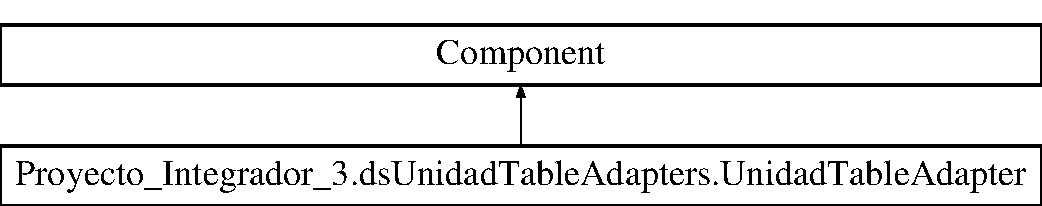
\includegraphics[height=2.000000cm]{df/d2f/class_proyecto___integrador__3_1_1ds_unidad_table_adapters_1_1_unidad_table_adapter}
\end{center}
\end{figure}
\subsection*{Métodos públicos}
\begin{DoxyCompactItemize}
\item 
\hyperlink{class_proyecto___integrador__3_1_1ds_unidad_table_adapters_1_1_unidad_table_adapter_acd553f95bf3151af8b6b4b877dab67e5}{Unidad\-Table\-Adapter} ()
\item 
virtual int \hyperlink{class_proyecto___integrador__3_1_1ds_unidad_table_adapters_1_1_unidad_table_adapter_a9b4cd452e334a4f1c9b587bc7d955f21}{Fill} (\hyperlink{class_proyecto___integrador__3_1_1ds_unidad_1_1_unidad_data_table}{ds\-Unidad.\-Unidad\-Data\-Table} data\-Table)
\item 
virtual \hyperlink{class_proyecto___integrador__3_1_1ds_unidad_1_1_unidad_data_table}{ds\-Unidad.\-Unidad\-Data\-Table} \hyperlink{class_proyecto___integrador__3_1_1ds_unidad_table_adapters_1_1_unidad_table_adapter_aa6880a92e220af9c45d78c8ad17a2b93}{Get\-Data} ()
\item 
virtual int \hyperlink{class_proyecto___integrador__3_1_1ds_unidad_table_adapters_1_1_unidad_table_adapter_ab66b8ee5e1153ac309331e6234ba7fad}{Update} (\hyperlink{class_proyecto___integrador__3_1_1ds_unidad_1_1_unidad_data_table}{ds\-Unidad.\-Unidad\-Data\-Table} data\-Table)
\item 
virtual int \hyperlink{class_proyecto___integrador__3_1_1ds_unidad_table_adapters_1_1_unidad_table_adapter_a5a943cac3ec30c6fa91b0059b8af7413}{Update} (\hyperlink{class_proyecto___integrador__3_1_1ds_unidad}{ds\-Unidad} data\-Set)
\item 
virtual int \hyperlink{class_proyecto___integrador__3_1_1ds_unidad_table_adapters_1_1_unidad_table_adapter_ae1789a516a249268c6230d4c71e45bd3}{Update} (global\-::\-System.\-Data.\-Data\-Row data\-Row)
\item 
virtual int \hyperlink{class_proyecto___integrador__3_1_1ds_unidad_table_adapters_1_1_unidad_table_adapter_a8008a1cbe0e208e9a6a582a950b93249}{Update} (global\-::\-System.\-Data.\-Data\-Row\mbox{[}$\,$\mbox{]} data\-Rows)
\item 
virtual int \hyperlink{class_proyecto___integrador__3_1_1ds_unidad_table_adapters_1_1_unidad_table_adapter_aa7acce7d136cd2115babbff7d95992f9}{Delete} (System.\-Guid Original\-\_\-\-Uid, string Original\-\_\-\-No\-Unidad)
\item 
virtual int \hyperlink{class_proyecto___integrador__3_1_1ds_unidad_table_adapters_1_1_unidad_table_adapter_ae9b51295d2db0d2f844a63f10ddd6346}{Insert} (System.\-Guid Uid, string No\-Unidad)
\item 
virtual int \hyperlink{class_proyecto___integrador__3_1_1ds_unidad_table_adapters_1_1_unidad_table_adapter_abfebbd44695319d75cd6ffaa8c3570fa}{Update} (System.\-Guid Uid, string No\-Unidad, System.\-Guid Original\-\_\-\-Uid, string Original\-\_\-\-No\-Unidad)
\item 
virtual int \hyperlink{class_proyecto___integrador__3_1_1ds_unidad_table_adapters_1_1_unidad_table_adapter_a9234374de0d3fa62b8c390465c024415}{Update} (string No\-Unidad, System.\-Guid Original\-\_\-\-Uid, string Original\-\_\-\-No\-Unidad)
\end{DoxyCompactItemize}
\subsection*{Propiedades}
\begin{DoxyCompactItemize}
\item 
global\-::\-System.\-Data.\-Sql\-Server\-Ce.\-Sql\-Ce\-Data\-Adapter \hyperlink{class_proyecto___integrador__3_1_1ds_unidad_table_adapters_1_1_unidad_table_adapter_a85041318aa5a0582ef54f4af0d332411}{Adapter}\hspace{0.3cm}{\ttfamily  \mbox{[}get\mbox{]}}
\item 
global\-::\-System.\-Data.\-Sql\-Server\-Ce.\-Sql\-Ce\-Connection \hyperlink{class_proyecto___integrador__3_1_1ds_unidad_table_adapters_1_1_unidad_table_adapter_a13a9c13fd0ce4e17d7f35891158864db}{Connection}\hspace{0.3cm}{\ttfamily  \mbox{[}get, set\mbox{]}}
\item 
global\-::\-System.\-Data.\-Sql\-Server\-Ce.\-Sql\-Ce\-Transaction \hyperlink{class_proyecto___integrador__3_1_1ds_unidad_table_adapters_1_1_unidad_table_adapter_a4bb3adb0822427867564cf7559b226cf}{Transaction}\hspace{0.3cm}{\ttfamily  \mbox{[}get, set\mbox{]}}
\item 
global\-::\-System.\-Data.\-Sql\-Server\-Ce.\-Sql\-Ce\-Command\mbox{[}$\,$\mbox{]} \hyperlink{class_proyecto___integrador__3_1_1ds_unidad_table_adapters_1_1_unidad_table_adapter_a1337b1ebd88dbe10e874222a4720ab71}{Command\-Collection}\hspace{0.3cm}{\ttfamily  \mbox{[}get\mbox{]}}
\item 
bool \hyperlink{class_proyecto___integrador__3_1_1ds_unidad_table_adapters_1_1_unidad_table_adapter_ac370b6e489375c1b39ec5d7f66472767}{Clear\-Before\-Fill}\hspace{0.3cm}{\ttfamily  \mbox{[}get, set\mbox{]}}
\end{DoxyCompactItemize}
\subsection*{Métodos privados}
\begin{DoxyCompactItemize}
\item 
void \hyperlink{class_proyecto___integrador__3_1_1ds_unidad_table_adapters_1_1_unidad_table_adapter_a206969f647e2d7297a8ac0d2f3dbc553}{Init\-Adapter} ()
\item 
void \hyperlink{class_proyecto___integrador__3_1_1ds_unidad_table_adapters_1_1_unidad_table_adapter_afd0c6a49e203d9fa6d0c1c2c613f0fe2}{Init\-Connection} ()
\item 
void \hyperlink{class_proyecto___integrador__3_1_1ds_unidad_table_adapters_1_1_unidad_table_adapter_a9679b7b20d598bf335bcd5c4aad67984}{Init\-Command\-Collection} ()
\end{DoxyCompactItemize}
\subsection*{Atributos privados}
\begin{DoxyCompactItemize}
\item 
global\-::\-System.\-Data.\-Sql\-Server\-Ce.\-Sql\-Ce\-Data\-Adapter \hyperlink{class_proyecto___integrador__3_1_1ds_unidad_table_adapters_1_1_unidad_table_adapter_ab399a596bea65cb98131fe8b2f74a979}{\-\_\-adapter}
\item 
global\-::\-System.\-Data.\-Sql\-Server\-Ce.\-Sql\-Ce\-Connection \hyperlink{class_proyecto___integrador__3_1_1ds_unidad_table_adapters_1_1_unidad_table_adapter_a1248a70b1ff6e674c43448a8a8afe9ab}{\-\_\-connection}
\item 
global\-::\-System.\-Data.\-Sql\-Server\-Ce.\-Sql\-Ce\-Transaction \hyperlink{class_proyecto___integrador__3_1_1ds_unidad_table_adapters_1_1_unidad_table_adapter_a902952d8f7e85197f0a9a3b00b0612ac}{\-\_\-transaction}
\item 
global\-::\-System.\-Data.\-Sql\-Server\-Ce.\-Sql\-Ce\-Command\mbox{[}$\,$\mbox{]} \hyperlink{class_proyecto___integrador__3_1_1ds_unidad_table_adapters_1_1_unidad_table_adapter_af19313099dd39bcd72211352e291e1fa}{\-\_\-command\-Collection}
\item 
bool \hyperlink{class_proyecto___integrador__3_1_1ds_unidad_table_adapters_1_1_unidad_table_adapter_aaffc291ca29a78e13577e8a89efa9551}{\-\_\-clear\-Before\-Fill}
\end{DoxyCompactItemize}


\subsection{Descripción detallada}
Represents the connection and commands used to retrieve and save data. 

/summary$>$ 

Definición en la línea 636 del archivo ds\-Unidad.\-Designer.\-cs.



\subsection{Documentación del constructor y destructor}
\hypertarget{class_proyecto___integrador__3_1_1ds_unidad_table_adapters_1_1_unidad_table_adapter_acd553f95bf3151af8b6b4b877dab67e5}{\index{Proyecto\-\_\-\-Integrador\-\_\-3\-::ds\-Unidad\-Table\-Adapters\-::\-Unidad\-Table\-Adapter@{Proyecto\-\_\-\-Integrador\-\_\-3\-::ds\-Unidad\-Table\-Adapters\-::\-Unidad\-Table\-Adapter}!Unidad\-Table\-Adapter@{Unidad\-Table\-Adapter}}
\index{Unidad\-Table\-Adapter@{Unidad\-Table\-Adapter}!Proyecto_Integrador_3::dsUnidadTableAdapters::UnidadTableAdapter@{Proyecto\-\_\-\-Integrador\-\_\-3\-::ds\-Unidad\-Table\-Adapters\-::\-Unidad\-Table\-Adapter}}
\subsubsection[{Unidad\-Table\-Adapter}]{\setlength{\rightskip}{0pt plus 5cm}Proyecto\-\_\-\-Integrador\-\_\-3.\-ds\-Unidad\-Table\-Adapters.\-Unidad\-Table\-Adapter.\-Unidad\-Table\-Adapter (
\begin{DoxyParamCaption}
{}
\end{DoxyParamCaption}
)}}\label{class_proyecto___integrador__3_1_1ds_unidad_table_adapters_1_1_unidad_table_adapter_acd553f95bf3151af8b6b4b877dab67e5}


Definición en la línea 650 del archivo ds\-Unidad.\-Designer.\-cs.


\begin{DoxyCode}
650                                     \{
651             this.\hyperlink{class_proyecto___integrador__3_1_1ds_unidad_table_adapters_1_1_unidad_table_adapter_ac370b6e489375c1b39ec5d7f66472767}{ClearBeforeFill} = \textcolor{keyword}{true};
652         \}
\end{DoxyCode}


\subsection{Documentación de las funciones miembro}
\hypertarget{class_proyecto___integrador__3_1_1ds_unidad_table_adapters_1_1_unidad_table_adapter_aa7acce7d136cd2115babbff7d95992f9}{\index{Proyecto\-\_\-\-Integrador\-\_\-3\-::ds\-Unidad\-Table\-Adapters\-::\-Unidad\-Table\-Adapter@{Proyecto\-\_\-\-Integrador\-\_\-3\-::ds\-Unidad\-Table\-Adapters\-::\-Unidad\-Table\-Adapter}!Delete@{Delete}}
\index{Delete@{Delete}!Proyecto_Integrador_3::dsUnidadTableAdapters::UnidadTableAdapter@{Proyecto\-\_\-\-Integrador\-\_\-3\-::ds\-Unidad\-Table\-Adapters\-::\-Unidad\-Table\-Adapter}}
\subsubsection[{Delete}]{\setlength{\rightskip}{0pt plus 5cm}virtual int Proyecto\-\_\-\-Integrador\-\_\-3.\-ds\-Unidad\-Table\-Adapters.\-Unidad\-Table\-Adapter.\-Delete (
\begin{DoxyParamCaption}
\item[{System.\-Guid}]{Original\-\_\-\-Uid, }
\item[{string}]{Original\-\_\-\-No\-Unidad}
\end{DoxyParamCaption}
)\hspace{0.3cm}{\ttfamily [virtual]}}}\label{class_proyecto___integrador__3_1_1ds_unidad_table_adapters_1_1_unidad_table_adapter_aa7acce7d136cd2115babbff7d95992f9}


Definición en la línea 849 del archivo ds\-Unidad.\-Designer.\-cs.


\begin{DoxyCode}
849                                                                                       \{
850             this.\hyperlink{class_proyecto___integrador__3_1_1ds_unidad_table_adapters_1_1_unidad_table_adapter_a85041318aa5a0582ef54f4af0d332411}{Adapter}.DeleteCommand.Parameters[0].Value = ((System.Guid)(Original\_Uid));
851             \textcolor{keywordflow}{if} ((Original\_NoUnidad == null)) \{
852                 \textcolor{keywordflow}{throw} \textcolor{keyword}{new} global::System.ArgumentNullException(\textcolor{stringliteral}{"Original\_NoUnidad"});
853             \}
854             \textcolor{keywordflow}{else} \{
855                 this.\hyperlink{class_proyecto___integrador__3_1_1ds_unidad_table_adapters_1_1_unidad_table_adapter_a85041318aa5a0582ef54f4af0d332411}{Adapter}.DeleteCommand.Parameters[1].Value = ((string)(Original\_NoUnidad));
856             \}
857             global::System.Data.ConnectionState previousConnectionState = this.
      \hyperlink{class_proyecto___integrador__3_1_1ds_unidad_table_adapters_1_1_unidad_table_adapter_a85041318aa5a0582ef54f4af0d332411}{Adapter}.DeleteCommand.Connection.State;
858             \textcolor{keywordflow}{if} (((this.\hyperlink{class_proyecto___integrador__3_1_1ds_unidad_table_adapters_1_1_unidad_table_adapter_a85041318aa5a0582ef54f4af0d332411}{Adapter}.DeleteCommand.Connection.State & global::System.Data.ConnectionState.
      Open) 
859                         != global::System.Data.ConnectionState.Open)) \{
860                 this.\hyperlink{class_proyecto___integrador__3_1_1ds_unidad_table_adapters_1_1_unidad_table_adapter_a85041318aa5a0582ef54f4af0d332411}{Adapter}.DeleteCommand.Connection.Open();
861             \}
862             \textcolor{keywordflow}{try} \{
863                 \textcolor{keywordtype}{int} returnValue = this.\hyperlink{class_proyecto___integrador__3_1_1ds_unidad_table_adapters_1_1_unidad_table_adapter_a85041318aa5a0582ef54f4af0d332411}{Adapter}.DeleteCommand.ExecuteNonQuery();
864                 \textcolor{keywordflow}{return} returnValue;
865             \}
866             \textcolor{keywordflow}{finally} \{
867                 \textcolor{keywordflow}{if} ((previousConnectionState == global::System.Data.ConnectionState.Closed)) \{
868                     this.\hyperlink{class_proyecto___integrador__3_1_1ds_unidad_table_adapters_1_1_unidad_table_adapter_a85041318aa5a0582ef54f4af0d332411}{Adapter}.DeleteCommand.Connection.Close();
869                 \}
870             \}
871         \}
\end{DoxyCode}
\hypertarget{class_proyecto___integrador__3_1_1ds_unidad_table_adapters_1_1_unidad_table_adapter_a9b4cd452e334a4f1c9b587bc7d955f21}{\index{Proyecto\-\_\-\-Integrador\-\_\-3\-::ds\-Unidad\-Table\-Adapters\-::\-Unidad\-Table\-Adapter@{Proyecto\-\_\-\-Integrador\-\_\-3\-::ds\-Unidad\-Table\-Adapters\-::\-Unidad\-Table\-Adapter}!Fill@{Fill}}
\index{Fill@{Fill}!Proyecto_Integrador_3::dsUnidadTableAdapters::UnidadTableAdapter@{Proyecto\-\_\-\-Integrador\-\_\-3\-::ds\-Unidad\-Table\-Adapters\-::\-Unidad\-Table\-Adapter}}
\subsubsection[{Fill}]{\setlength{\rightskip}{0pt plus 5cm}virtual int Proyecto\-\_\-\-Integrador\-\_\-3.\-ds\-Unidad\-Table\-Adapters.\-Unidad\-Table\-Adapter.\-Fill (
\begin{DoxyParamCaption}
\item[{{\bf ds\-Unidad.\-Unidad\-Data\-Table}}]{data\-Table}
\end{DoxyParamCaption}
)\hspace{0.3cm}{\ttfamily [virtual]}}}\label{class_proyecto___integrador__3_1_1ds_unidad_table_adapters_1_1_unidad_table_adapter_a9b4cd452e334a4f1c9b587bc7d955f21}


Definición en la línea 796 del archivo ds\-Unidad.\-Designer.\-cs.


\begin{DoxyCode}
796                                                                     \{
797             this.\hyperlink{class_proyecto___integrador__3_1_1ds_unidad_table_adapters_1_1_unidad_table_adapter_a85041318aa5a0582ef54f4af0d332411}{Adapter}.SelectCommand = this.\hyperlink{class_proyecto___integrador__3_1_1ds_unidad_table_adapters_1_1_unidad_table_adapter_a1337b1ebd88dbe10e874222a4720ab71}{CommandCollection}[0];
798             \textcolor{keywordflow}{if} ((this.\hyperlink{class_proyecto___integrador__3_1_1ds_unidad_table_adapters_1_1_unidad_table_adapter_ac370b6e489375c1b39ec5d7f66472767}{ClearBeforeFill} == \textcolor{keyword}{true})) \{
799                 dataTable.Clear();
800             \}
801             \textcolor{keywordtype}{int} returnValue = this.\hyperlink{class_proyecto___integrador__3_1_1ds_unidad_table_adapters_1_1_unidad_table_adapter_a85041318aa5a0582ef54f4af0d332411}{Adapter}.Fill(dataTable);
802             \textcolor{keywordflow}{return} returnValue;
803         \}
\end{DoxyCode}
\hypertarget{class_proyecto___integrador__3_1_1ds_unidad_table_adapters_1_1_unidad_table_adapter_aa6880a92e220af9c45d78c8ad17a2b93}{\index{Proyecto\-\_\-\-Integrador\-\_\-3\-::ds\-Unidad\-Table\-Adapters\-::\-Unidad\-Table\-Adapter@{Proyecto\-\_\-\-Integrador\-\_\-3\-::ds\-Unidad\-Table\-Adapters\-::\-Unidad\-Table\-Adapter}!Get\-Data@{Get\-Data}}
\index{Get\-Data@{Get\-Data}!Proyecto_Integrador_3::dsUnidadTableAdapters::UnidadTableAdapter@{Proyecto\-\_\-\-Integrador\-\_\-3\-::ds\-Unidad\-Table\-Adapters\-::\-Unidad\-Table\-Adapter}}
\subsubsection[{Get\-Data}]{\setlength{\rightskip}{0pt plus 5cm}virtual {\bf ds\-Unidad.\-Unidad\-Data\-Table} Proyecto\-\_\-\-Integrador\-\_\-3.\-ds\-Unidad\-Table\-Adapters.\-Unidad\-Table\-Adapter.\-Get\-Data (
\begin{DoxyParamCaption}
{}
\end{DoxyParamCaption}
)\hspace{0.3cm}{\ttfamily [virtual]}}}\label{class_proyecto___integrador__3_1_1ds_unidad_table_adapters_1_1_unidad_table_adapter_aa6880a92e220af9c45d78c8ad17a2b93}


Definición en la línea 809 del archivo ds\-Unidad.\-Designer.\-cs.


\begin{DoxyCode}
809                                                           \{
810             this.\hyperlink{class_proyecto___integrador__3_1_1ds_unidad_table_adapters_1_1_unidad_table_adapter_a85041318aa5a0582ef54f4af0d332411}{Adapter}.SelectCommand = this.\hyperlink{class_proyecto___integrador__3_1_1ds_unidad_table_adapters_1_1_unidad_table_adapter_a1337b1ebd88dbe10e874222a4720ab71}{CommandCollection}[0];
811             dsUnidad.UnidadDataTable dataTable = \textcolor{keyword}{new} dsUnidad.UnidadDataTable();
812             this.\hyperlink{class_proyecto___integrador__3_1_1ds_unidad_table_adapters_1_1_unidad_table_adapter_a85041318aa5a0582ef54f4af0d332411}{Adapter}.Fill(dataTable);
813             \textcolor{keywordflow}{return} dataTable;
814         \}
\end{DoxyCode}
\hypertarget{class_proyecto___integrador__3_1_1ds_unidad_table_adapters_1_1_unidad_table_adapter_a206969f647e2d7297a8ac0d2f3dbc553}{\index{Proyecto\-\_\-\-Integrador\-\_\-3\-::ds\-Unidad\-Table\-Adapters\-::\-Unidad\-Table\-Adapter@{Proyecto\-\_\-\-Integrador\-\_\-3\-::ds\-Unidad\-Table\-Adapters\-::\-Unidad\-Table\-Adapter}!Init\-Adapter@{Init\-Adapter}}
\index{Init\-Adapter@{Init\-Adapter}!Proyecto_Integrador_3::dsUnidadTableAdapters::UnidadTableAdapter@{Proyecto\-\_\-\-Integrador\-\_\-3\-::ds\-Unidad\-Table\-Adapters\-::\-Unidad\-Table\-Adapter}}
\subsubsection[{Init\-Adapter}]{\setlength{\rightskip}{0pt plus 5cm}void Proyecto\-\_\-\-Integrador\-\_\-3.\-ds\-Unidad\-Table\-Adapters.\-Unidad\-Table\-Adapter.\-Init\-Adapter (
\begin{DoxyParamCaption}
{}
\end{DoxyParamCaption}
)\hspace{0.3cm}{\ttfamily [private]}}}\label{class_proyecto___integrador__3_1_1ds_unidad_table_adapters_1_1_unidad_table_adapter_a206969f647e2d7297a8ac0d2f3dbc553}


Definición en la línea 743 del archivo ds\-Unidad.\-Designer.\-cs.


\begin{DoxyCode}
743                                    \{
744             this.\hyperlink{class_proyecto___integrador__3_1_1ds_unidad_table_adapters_1_1_unidad_table_adapter_ab399a596bea65cb98131fe8b2f74a979}{\_adapter} = \textcolor{keyword}{new} global::System.Data.SqlServerCe.SqlCeDataAdapter();
745             global::System.Data.Common.DataTableMapping tableMapping = \textcolor{keyword}{new} global::System.Data.Common.
      DataTableMapping();
746             tableMapping.SourceTable = \textcolor{stringliteral}{"Table"};
747             tableMapping.DataSetTable = \textcolor{stringliteral}{"Unidad"};
748             tableMapping.ColumnMappings.Add(\textcolor{stringliteral}{"Uid"}, \textcolor{stringliteral}{"Uid"});
749             tableMapping.ColumnMappings.Add(\textcolor{stringliteral}{"NoUnidad"}, \textcolor{stringliteral}{"NoUnidad"});
750             this.\hyperlink{class_proyecto___integrador__3_1_1ds_unidad_table_adapters_1_1_unidad_table_adapter_ab399a596bea65cb98131fe8b2f74a979}{\_adapter}.TableMappings.Add(tableMapping);
751             this.\hyperlink{class_proyecto___integrador__3_1_1ds_unidad_table_adapters_1_1_unidad_table_adapter_ab399a596bea65cb98131fe8b2f74a979}{\_adapter}.DeleteCommand = \textcolor{keyword}{new} global::System.Data.SqlServerCe.SqlCeCommand();
752             this.\hyperlink{class_proyecto___integrador__3_1_1ds_unidad_table_adapters_1_1_unidad_table_adapter_ab399a596bea65cb98131fe8b2f74a979}{\_adapter}.DeleteCommand.Connection = this.\hyperlink{class_proyecto___integrador__3_1_1ds_unidad_table_adapters_1_1_unidad_table_adapter_a13a9c13fd0ce4e17d7f35891158864db}{Connection};
753             this.\hyperlink{class_proyecto___integrador__3_1_1ds_unidad_table_adapters_1_1_unidad_table_adapter_ab399a596bea65cb98131fe8b2f74a979}{\_adapter}.DeleteCommand.CommandText = \textcolor{stringliteral}{"DELETE FROM [Unidad] WHERE (([Uid] =
       @Original\_Uid) AND ([NoUnidad] = @Original\_N"} +
754                 \textcolor{stringliteral}{"oUnidad))"};
755             this.\hyperlink{class_proyecto___integrador__3_1_1ds_unidad_table_adapters_1_1_unidad_table_adapter_ab399a596bea65cb98131fe8b2f74a979}{\_adapter}.DeleteCommand.CommandType = global::System.Data.CommandType.Text;
756             this.\hyperlink{class_proyecto___integrador__3_1_1ds_unidad_table_adapters_1_1_unidad_table_adapter_ab399a596bea65cb98131fe8b2f74a979}{\_adapter}.DeleteCommand.Parameters.Add(\textcolor{keyword}{new} global::System.Data.SqlServerCe.
      SqlCeParameter(\textcolor{stringliteral}{"@Original\_Uid"}, global::System.Data.SqlDbType.UniqueIdentifier, 0, global::System.Data.
      ParameterDirection.Input, \textcolor{keyword}{true}, 0, 0, \textcolor{stringliteral}{"Uid"}, global::System.Data.DataRowVersion.Original, null));
757             this.\hyperlink{class_proyecto___integrador__3_1_1ds_unidad_table_adapters_1_1_unidad_table_adapter_ab399a596bea65cb98131fe8b2f74a979}{\_adapter}.DeleteCommand.Parameters.Add(\textcolor{keyword}{new} global::System.Data.SqlServerCe.
      SqlCeParameter(\textcolor{stringliteral}{"@Original\_NoUnidad"}, global::System.Data.SqlDbType.NVarChar, 0, global::System.Data.
      ParameterDirection.Input, \textcolor{keyword}{true}, 0, 0, \textcolor{stringliteral}{"NoUnidad"}, global::System.Data.DataRowVersion.Original, null));
758             this.\hyperlink{class_proyecto___integrador__3_1_1ds_unidad_table_adapters_1_1_unidad_table_adapter_ab399a596bea65cb98131fe8b2f74a979}{\_adapter}.InsertCommand = \textcolor{keyword}{new} global::System.Data.SqlServerCe.SqlCeCommand();
759             this.\hyperlink{class_proyecto___integrador__3_1_1ds_unidad_table_adapters_1_1_unidad_table_adapter_ab399a596bea65cb98131fe8b2f74a979}{\_adapter}.InsertCommand.Connection = this.\hyperlink{class_proyecto___integrador__3_1_1ds_unidad_table_adapters_1_1_unidad_table_adapter_a13a9c13fd0ce4e17d7f35891158864db}{Connection};
760             this.\hyperlink{class_proyecto___integrador__3_1_1ds_unidad_table_adapters_1_1_unidad_table_adapter_ab399a596bea65cb98131fe8b2f74a979}{\_adapter}.InsertCommand.CommandText = \textcolor{stringliteral}{"INSERT INTO [Unidad] ([Uid], [NoUnidad])
       VALUES (@Uid, @NoUnidad)"};
761             this.\hyperlink{class_proyecto___integrador__3_1_1ds_unidad_table_adapters_1_1_unidad_table_adapter_ab399a596bea65cb98131fe8b2f74a979}{\_adapter}.InsertCommand.CommandType = global::System.Data.CommandType.Text;
762             this.\hyperlink{class_proyecto___integrador__3_1_1ds_unidad_table_adapters_1_1_unidad_table_adapter_ab399a596bea65cb98131fe8b2f74a979}{\_adapter}.InsertCommand.Parameters.Add(\textcolor{keyword}{new} global::System.Data.SqlServerCe.
      SqlCeParameter(\textcolor{stringliteral}{"@Uid"}, global::System.Data.SqlDbType.UniqueIdentifier, 0, global::System.Data.ParameterDirection.
      Input, \textcolor{keyword}{true}, 0, 0, \textcolor{stringliteral}{"Uid"}, global::System.Data.DataRowVersion.Current, null));
763             this.\hyperlink{class_proyecto___integrador__3_1_1ds_unidad_table_adapters_1_1_unidad_table_adapter_ab399a596bea65cb98131fe8b2f74a979}{\_adapter}.InsertCommand.Parameters.Add(\textcolor{keyword}{new} global::System.Data.SqlServerCe.
      SqlCeParameter(\textcolor{stringliteral}{"@NoUnidad"}, global::System.Data.SqlDbType.NVarChar, 0, global::System.Data.ParameterDirection.Input,
       \textcolor{keyword}{true}, 0, 0, \textcolor{stringliteral}{"NoUnidad"}, global::System.Data.DataRowVersion.Current, null));
764             this.\hyperlink{class_proyecto___integrador__3_1_1ds_unidad_table_adapters_1_1_unidad_table_adapter_ab399a596bea65cb98131fe8b2f74a979}{\_adapter}.UpdateCommand = \textcolor{keyword}{new} global::System.Data.SqlServerCe.SqlCeCommand();
765             this.\hyperlink{class_proyecto___integrador__3_1_1ds_unidad_table_adapters_1_1_unidad_table_adapter_ab399a596bea65cb98131fe8b2f74a979}{\_adapter}.UpdateCommand.Connection = this.\hyperlink{class_proyecto___integrador__3_1_1ds_unidad_table_adapters_1_1_unidad_table_adapter_a13a9c13fd0ce4e17d7f35891158864db}{Connection};
766             this.\hyperlink{class_proyecto___integrador__3_1_1ds_unidad_table_adapters_1_1_unidad_table_adapter_ab399a596bea65cb98131fe8b2f74a979}{\_adapter}.UpdateCommand.CommandText = \textcolor{stringliteral}{"UPDATE [Unidad] SET [Uid] = @Uid, [NoUnidad]
       = @NoUnidad WHERE (([Uid] = @Origina"} +
767                 \textcolor{stringliteral}{"l\_Uid) AND ([NoUnidad] = @Original\_NoUnidad))"};
768             this.\hyperlink{class_proyecto___integrador__3_1_1ds_unidad_table_adapters_1_1_unidad_table_adapter_ab399a596bea65cb98131fe8b2f74a979}{\_adapter}.UpdateCommand.CommandType = global::System.Data.CommandType.Text;
769             this.\hyperlink{class_proyecto___integrador__3_1_1ds_unidad_table_adapters_1_1_unidad_table_adapter_ab399a596bea65cb98131fe8b2f74a979}{\_adapter}.UpdateCommand.Parameters.Add(\textcolor{keyword}{new} global::System.Data.SqlServerCe.
      SqlCeParameter(\textcolor{stringliteral}{"@Uid"}, global::System.Data.SqlDbType.UniqueIdentifier, 0, global::System.Data.ParameterDirection.
      Input, \textcolor{keyword}{true}, 0, 0, \textcolor{stringliteral}{"Uid"}, global::System.Data.DataRowVersion.Current, null));
770             this.\hyperlink{class_proyecto___integrador__3_1_1ds_unidad_table_adapters_1_1_unidad_table_adapter_ab399a596bea65cb98131fe8b2f74a979}{\_adapter}.UpdateCommand.Parameters.Add(\textcolor{keyword}{new} global::System.Data.SqlServerCe.
      SqlCeParameter(\textcolor{stringliteral}{"@NoUnidad"}, global::System.Data.SqlDbType.NVarChar, 0, global::System.Data.ParameterDirection.Input,
       \textcolor{keyword}{true}, 0, 0, \textcolor{stringliteral}{"NoUnidad"}, global::System.Data.DataRowVersion.Current, null));
771             this.\hyperlink{class_proyecto___integrador__3_1_1ds_unidad_table_adapters_1_1_unidad_table_adapter_ab399a596bea65cb98131fe8b2f74a979}{\_adapter}.UpdateCommand.Parameters.Add(\textcolor{keyword}{new} global::System.Data.SqlServerCe.
      SqlCeParameter(\textcolor{stringliteral}{"@Original\_Uid"}, global::System.Data.SqlDbType.UniqueIdentifier, 0, global::System.Data.
      ParameterDirection.Input, \textcolor{keyword}{true}, 0, 0, \textcolor{stringliteral}{"Uid"}, global::System.Data.DataRowVersion.Original, null));
772             this.\hyperlink{class_proyecto___integrador__3_1_1ds_unidad_table_adapters_1_1_unidad_table_adapter_ab399a596bea65cb98131fe8b2f74a979}{\_adapter}.UpdateCommand.Parameters.Add(\textcolor{keyword}{new} global::System.Data.SqlServerCe.
      SqlCeParameter(\textcolor{stringliteral}{"@Original\_NoUnidad"}, global::System.Data.SqlDbType.NVarChar, 0, global::System.Data.
      ParameterDirection.Input, \textcolor{keyword}{true}, 0, 0, \textcolor{stringliteral}{"NoUnidad"}, global::System.Data.DataRowVersion.Original, null));
773         \}
\end{DoxyCode}
\hypertarget{class_proyecto___integrador__3_1_1ds_unidad_table_adapters_1_1_unidad_table_adapter_a9679b7b20d598bf335bcd5c4aad67984}{\index{Proyecto\-\_\-\-Integrador\-\_\-3\-::ds\-Unidad\-Table\-Adapters\-::\-Unidad\-Table\-Adapter@{Proyecto\-\_\-\-Integrador\-\_\-3\-::ds\-Unidad\-Table\-Adapters\-::\-Unidad\-Table\-Adapter}!Init\-Command\-Collection@{Init\-Command\-Collection}}
\index{Init\-Command\-Collection@{Init\-Command\-Collection}!Proyecto_Integrador_3::dsUnidadTableAdapters::UnidadTableAdapter@{Proyecto\-\_\-\-Integrador\-\_\-3\-::ds\-Unidad\-Table\-Adapters\-::\-Unidad\-Table\-Adapter}}
\subsubsection[{Init\-Command\-Collection}]{\setlength{\rightskip}{0pt plus 5cm}void Proyecto\-\_\-\-Integrador\-\_\-3.\-ds\-Unidad\-Table\-Adapters.\-Unidad\-Table\-Adapter.\-Init\-Command\-Collection (
\begin{DoxyParamCaption}
{}
\end{DoxyParamCaption}
)\hspace{0.3cm}{\ttfamily [private]}}}\label{class_proyecto___integrador__3_1_1ds_unidad_table_adapters_1_1_unidad_table_adapter_a9679b7b20d598bf335bcd5c4aad67984}


Definición en la línea 784 del archivo ds\-Unidad.\-Designer.\-cs.


\begin{DoxyCode}
784                                              \{
785             this.\hyperlink{class_proyecto___integrador__3_1_1ds_unidad_table_adapters_1_1_unidad_table_adapter_af19313099dd39bcd72211352e291e1fa}{\_commandCollection} = \textcolor{keyword}{new} global::System.Data.SqlServerCe.SqlCeCommand[1]
      ;
786             this.\hyperlink{class_proyecto___integrador__3_1_1ds_unidad_table_adapters_1_1_unidad_table_adapter_af19313099dd39bcd72211352e291e1fa}{\_commandCollection}[0] = \textcolor{keyword}{new} global::System.Data.SqlServerCe.SqlCeCommand
      ();
787             this.\hyperlink{class_proyecto___integrador__3_1_1ds_unidad_table_adapters_1_1_unidad_table_adapter_af19313099dd39bcd72211352e291e1fa}{\_commandCollection}[0].Connection = this.
      \hyperlink{class_proyecto___integrador__3_1_1ds_unidad_table_adapters_1_1_unidad_table_adapter_a13a9c13fd0ce4e17d7f35891158864db}{Connection};
788             this.\hyperlink{class_proyecto___integrador__3_1_1ds_unidad_table_adapters_1_1_unidad_table_adapter_af19313099dd39bcd72211352e291e1fa}{\_commandCollection}[0].CommandText = \textcolor{stringliteral}{"SELECT Unidad.*\(\backslash\)r\(\backslash\)nFROM     Unidad"}
      ;
789             this.\hyperlink{class_proyecto___integrador__3_1_1ds_unidad_table_adapters_1_1_unidad_table_adapter_af19313099dd39bcd72211352e291e1fa}{\_commandCollection}[0].CommandType = global::System.Data.CommandType.Text
      ;
790         \}
\end{DoxyCode}
\hypertarget{class_proyecto___integrador__3_1_1ds_unidad_table_adapters_1_1_unidad_table_adapter_afd0c6a49e203d9fa6d0c1c2c613f0fe2}{\index{Proyecto\-\_\-\-Integrador\-\_\-3\-::ds\-Unidad\-Table\-Adapters\-::\-Unidad\-Table\-Adapter@{Proyecto\-\_\-\-Integrador\-\_\-3\-::ds\-Unidad\-Table\-Adapters\-::\-Unidad\-Table\-Adapter}!Init\-Connection@{Init\-Connection}}
\index{Init\-Connection@{Init\-Connection}!Proyecto_Integrador_3::dsUnidadTableAdapters::UnidadTableAdapter@{Proyecto\-\_\-\-Integrador\-\_\-3\-::ds\-Unidad\-Table\-Adapters\-::\-Unidad\-Table\-Adapter}}
\subsubsection[{Init\-Connection}]{\setlength{\rightskip}{0pt plus 5cm}void Proyecto\-\_\-\-Integrador\-\_\-3.\-ds\-Unidad\-Table\-Adapters.\-Unidad\-Table\-Adapter.\-Init\-Connection (
\begin{DoxyParamCaption}
{}
\end{DoxyParamCaption}
)\hspace{0.3cm}{\ttfamily [private]}}}\label{class_proyecto___integrador__3_1_1ds_unidad_table_adapters_1_1_unidad_table_adapter_afd0c6a49e203d9fa6d0c1c2c613f0fe2}


Definición en la línea 777 del archivo ds\-Unidad.\-Designer.\-cs.


\begin{DoxyCode}
777                                       \{
778             this.\hyperlink{class_proyecto___integrador__3_1_1ds_unidad_table_adapters_1_1_unidad_table_adapter_a1248a70b1ff6e674c43448a8a8afe9ab}{\_connection} = \textcolor{keyword}{new} global::System.Data.SqlServerCe.SqlCeConnection();
779             this.\hyperlink{class_proyecto___integrador__3_1_1ds_unidad_table_adapters_1_1_unidad_table_adapter_a1248a70b1ff6e674c43448a8a8afe9ab}{\_connection}.ConnectionString = global::Proyecto\_Integrador\_3.Properties.
      Settings.Default.ProyectoIntegradorConnectionString;
780         \}
\end{DoxyCode}
\hypertarget{class_proyecto___integrador__3_1_1ds_unidad_table_adapters_1_1_unidad_table_adapter_ae9b51295d2db0d2f844a63f10ddd6346}{\index{Proyecto\-\_\-\-Integrador\-\_\-3\-::ds\-Unidad\-Table\-Adapters\-::\-Unidad\-Table\-Adapter@{Proyecto\-\_\-\-Integrador\-\_\-3\-::ds\-Unidad\-Table\-Adapters\-::\-Unidad\-Table\-Adapter}!Insert@{Insert}}
\index{Insert@{Insert}!Proyecto_Integrador_3::dsUnidadTableAdapters::UnidadTableAdapter@{Proyecto\-\_\-\-Integrador\-\_\-3\-::ds\-Unidad\-Table\-Adapters\-::\-Unidad\-Table\-Adapter}}
\subsubsection[{Insert}]{\setlength{\rightskip}{0pt plus 5cm}virtual int Proyecto\-\_\-\-Integrador\-\_\-3.\-ds\-Unidad\-Table\-Adapters.\-Unidad\-Table\-Adapter.\-Insert (
\begin{DoxyParamCaption}
\item[{System.\-Guid}]{Uid, }
\item[{string}]{No\-Unidad}
\end{DoxyParamCaption}
)\hspace{0.3cm}{\ttfamily [virtual]}}}\label{class_proyecto___integrador__3_1_1ds_unidad_table_adapters_1_1_unidad_table_adapter_ae9b51295d2db0d2f844a63f10ddd6346}


Definición en la línea 877 del archivo ds\-Unidad.\-Designer.\-cs.


\begin{DoxyCode}
877                                                                     \{
878             this.\hyperlink{class_proyecto___integrador__3_1_1ds_unidad_table_adapters_1_1_unidad_table_adapter_a85041318aa5a0582ef54f4af0d332411}{Adapter}.InsertCommand.Parameters[0].Value = ((System.Guid)(Uid));
879             \textcolor{keywordflow}{if} ((NoUnidad == null)) \{
880                 \textcolor{keywordflow}{throw} \textcolor{keyword}{new} global::System.ArgumentNullException(\textcolor{stringliteral}{"NoUnidad"});
881             \}
882             \textcolor{keywordflow}{else} \{
883                 this.\hyperlink{class_proyecto___integrador__3_1_1ds_unidad_table_adapters_1_1_unidad_table_adapter_a85041318aa5a0582ef54f4af0d332411}{Adapter}.InsertCommand.Parameters[1].Value = ((string)(NoUnidad));
884             \}
885             global::System.Data.ConnectionState previousConnectionState = this.
      \hyperlink{class_proyecto___integrador__3_1_1ds_unidad_table_adapters_1_1_unidad_table_adapter_a85041318aa5a0582ef54f4af0d332411}{Adapter}.InsertCommand.Connection.State;
886             \textcolor{keywordflow}{if} (((this.\hyperlink{class_proyecto___integrador__3_1_1ds_unidad_table_adapters_1_1_unidad_table_adapter_a85041318aa5a0582ef54f4af0d332411}{Adapter}.InsertCommand.Connection.State & global::System.Data.ConnectionState.
      Open) 
887                         != global::System.Data.ConnectionState.Open)) \{
888                 this.\hyperlink{class_proyecto___integrador__3_1_1ds_unidad_table_adapters_1_1_unidad_table_adapter_a85041318aa5a0582ef54f4af0d332411}{Adapter}.InsertCommand.Connection.Open();
889             \}
890             \textcolor{keywordflow}{try} \{
891                 \textcolor{keywordtype}{int} returnValue = this.\hyperlink{class_proyecto___integrador__3_1_1ds_unidad_table_adapters_1_1_unidad_table_adapter_a85041318aa5a0582ef54f4af0d332411}{Adapter}.InsertCommand.ExecuteNonQuery();
892                 \textcolor{keywordflow}{return} returnValue;
893             \}
894             \textcolor{keywordflow}{finally} \{
895                 \textcolor{keywordflow}{if} ((previousConnectionState == global::System.Data.ConnectionState.Closed)) \{
896                     this.\hyperlink{class_proyecto___integrador__3_1_1ds_unidad_table_adapters_1_1_unidad_table_adapter_a85041318aa5a0582ef54f4af0d332411}{Adapter}.InsertCommand.Connection.Close();
897                 \}
898             \}
899         \}
\end{DoxyCode}
\hypertarget{class_proyecto___integrador__3_1_1ds_unidad_table_adapters_1_1_unidad_table_adapter_ab66b8ee5e1153ac309331e6234ba7fad}{\index{Proyecto\-\_\-\-Integrador\-\_\-3\-::ds\-Unidad\-Table\-Adapters\-::\-Unidad\-Table\-Adapter@{Proyecto\-\_\-\-Integrador\-\_\-3\-::ds\-Unidad\-Table\-Adapters\-::\-Unidad\-Table\-Adapter}!Update@{Update}}
\index{Update@{Update}!Proyecto_Integrador_3::dsUnidadTableAdapters::UnidadTableAdapter@{Proyecto\-\_\-\-Integrador\-\_\-3\-::ds\-Unidad\-Table\-Adapters\-::\-Unidad\-Table\-Adapter}}
\subsubsection[{Update}]{\setlength{\rightskip}{0pt plus 5cm}virtual int Proyecto\-\_\-\-Integrador\-\_\-3.\-ds\-Unidad\-Table\-Adapters.\-Unidad\-Table\-Adapter.\-Update (
\begin{DoxyParamCaption}
\item[{{\bf ds\-Unidad.\-Unidad\-Data\-Table}}]{data\-Table}
\end{DoxyParamCaption}
)\hspace{0.3cm}{\ttfamily [virtual]}}}\label{class_proyecto___integrador__3_1_1ds_unidad_table_adapters_1_1_unidad_table_adapter_ab66b8ee5e1153ac309331e6234ba7fad}


Definición en la línea 819 del archivo ds\-Unidad.\-Designer.\-cs.


\begin{DoxyCode}
819                                                                       \{
820             \textcolor{keywordflow}{return} this.\hyperlink{class_proyecto___integrador__3_1_1ds_unidad_table_adapters_1_1_unidad_table_adapter_a85041318aa5a0582ef54f4af0d332411}{Adapter}.Update(dataTable);
821         \}
\end{DoxyCode}
\hypertarget{class_proyecto___integrador__3_1_1ds_unidad_table_adapters_1_1_unidad_table_adapter_a5a943cac3ec30c6fa91b0059b8af7413}{\index{Proyecto\-\_\-\-Integrador\-\_\-3\-::ds\-Unidad\-Table\-Adapters\-::\-Unidad\-Table\-Adapter@{Proyecto\-\_\-\-Integrador\-\_\-3\-::ds\-Unidad\-Table\-Adapters\-::\-Unidad\-Table\-Adapter}!Update@{Update}}
\index{Update@{Update}!Proyecto_Integrador_3::dsUnidadTableAdapters::UnidadTableAdapter@{Proyecto\-\_\-\-Integrador\-\_\-3\-::ds\-Unidad\-Table\-Adapters\-::\-Unidad\-Table\-Adapter}}
\subsubsection[{Update}]{\setlength{\rightskip}{0pt plus 5cm}virtual int Proyecto\-\_\-\-Integrador\-\_\-3.\-ds\-Unidad\-Table\-Adapters.\-Unidad\-Table\-Adapter.\-Update (
\begin{DoxyParamCaption}
\item[{{\bf ds\-Unidad}}]{data\-Set}
\end{DoxyParamCaption}
)\hspace{0.3cm}{\ttfamily [virtual]}}}\label{class_proyecto___integrador__3_1_1ds_unidad_table_adapters_1_1_unidad_table_adapter_a5a943cac3ec30c6fa91b0059b8af7413}


Definición en la línea 826 del archivo ds\-Unidad.\-Designer.\-cs.


\begin{DoxyCode}
826                                                     \{
827             \textcolor{keywordflow}{return} this.\hyperlink{class_proyecto___integrador__3_1_1ds_unidad_table_adapters_1_1_unidad_table_adapter_a85041318aa5a0582ef54f4af0d332411}{Adapter}.Update(dataSet, \textcolor{stringliteral}{"Unidad"});
828         \}
\end{DoxyCode}
\hypertarget{class_proyecto___integrador__3_1_1ds_unidad_table_adapters_1_1_unidad_table_adapter_ae1789a516a249268c6230d4c71e45bd3}{\index{Proyecto\-\_\-\-Integrador\-\_\-3\-::ds\-Unidad\-Table\-Adapters\-::\-Unidad\-Table\-Adapter@{Proyecto\-\_\-\-Integrador\-\_\-3\-::ds\-Unidad\-Table\-Adapters\-::\-Unidad\-Table\-Adapter}!Update@{Update}}
\index{Update@{Update}!Proyecto_Integrador_3::dsUnidadTableAdapters::UnidadTableAdapter@{Proyecto\-\_\-\-Integrador\-\_\-3\-::ds\-Unidad\-Table\-Adapters\-::\-Unidad\-Table\-Adapter}}
\subsubsection[{Update}]{\setlength{\rightskip}{0pt plus 5cm}virtual int Proyecto\-\_\-\-Integrador\-\_\-3.\-ds\-Unidad\-Table\-Adapters.\-Unidad\-Table\-Adapter.\-Update (
\begin{DoxyParamCaption}
\item[{global\-::\-System.\-Data.\-Data\-Row}]{data\-Row}
\end{DoxyParamCaption}
)\hspace{0.3cm}{\ttfamily [virtual]}}}\label{class_proyecto___integrador__3_1_1ds_unidad_table_adapters_1_1_unidad_table_adapter_ae1789a516a249268c6230d4c71e45bd3}


Definición en la línea 833 del archivo ds\-Unidad.\-Designer.\-cs.


\begin{DoxyCode}
833                                                                      \{
834             \textcolor{keywordflow}{return} this.\hyperlink{class_proyecto___integrador__3_1_1ds_unidad_table_adapters_1_1_unidad_table_adapter_a85041318aa5a0582ef54f4af0d332411}{Adapter}.Update(\textcolor{keyword}{new} global::System.Data.DataRow[] \{
835                         dataRow\});
836         \}
\end{DoxyCode}
\hypertarget{class_proyecto___integrador__3_1_1ds_unidad_table_adapters_1_1_unidad_table_adapter_a8008a1cbe0e208e9a6a582a950b93249}{\index{Proyecto\-\_\-\-Integrador\-\_\-3\-::ds\-Unidad\-Table\-Adapters\-::\-Unidad\-Table\-Adapter@{Proyecto\-\_\-\-Integrador\-\_\-3\-::ds\-Unidad\-Table\-Adapters\-::\-Unidad\-Table\-Adapter}!Update@{Update}}
\index{Update@{Update}!Proyecto_Integrador_3::dsUnidadTableAdapters::UnidadTableAdapter@{Proyecto\-\_\-\-Integrador\-\_\-3\-::ds\-Unidad\-Table\-Adapters\-::\-Unidad\-Table\-Adapter}}
\subsubsection[{Update}]{\setlength{\rightskip}{0pt plus 5cm}virtual int Proyecto\-\_\-\-Integrador\-\_\-3.\-ds\-Unidad\-Table\-Adapters.\-Unidad\-Table\-Adapter.\-Update (
\begin{DoxyParamCaption}
\item[{global\-::\-System.\-Data.\-Data\-Row\mbox{[}$\,$\mbox{]}}]{data\-Rows}
\end{DoxyParamCaption}
)\hspace{0.3cm}{\ttfamily [virtual]}}}\label{class_proyecto___integrador__3_1_1ds_unidad_table_adapters_1_1_unidad_table_adapter_a8008a1cbe0e208e9a6a582a950b93249}


Definición en la línea 841 del archivo ds\-Unidad.\-Designer.\-cs.


\begin{DoxyCode}
841                                                                         \{
842             \textcolor{keywordflow}{return} this.\hyperlink{class_proyecto___integrador__3_1_1ds_unidad_table_adapters_1_1_unidad_table_adapter_a85041318aa5a0582ef54f4af0d332411}{Adapter}.Update(dataRows);
843         \}
\end{DoxyCode}
\hypertarget{class_proyecto___integrador__3_1_1ds_unidad_table_adapters_1_1_unidad_table_adapter_abfebbd44695319d75cd6ffaa8c3570fa}{\index{Proyecto\-\_\-\-Integrador\-\_\-3\-::ds\-Unidad\-Table\-Adapters\-::\-Unidad\-Table\-Adapter@{Proyecto\-\_\-\-Integrador\-\_\-3\-::ds\-Unidad\-Table\-Adapters\-::\-Unidad\-Table\-Adapter}!Update@{Update}}
\index{Update@{Update}!Proyecto_Integrador_3::dsUnidadTableAdapters::UnidadTableAdapter@{Proyecto\-\_\-\-Integrador\-\_\-3\-::ds\-Unidad\-Table\-Adapters\-::\-Unidad\-Table\-Adapter}}
\subsubsection[{Update}]{\setlength{\rightskip}{0pt plus 5cm}virtual int Proyecto\-\_\-\-Integrador\-\_\-3.\-ds\-Unidad\-Table\-Adapters.\-Unidad\-Table\-Adapter.\-Update (
\begin{DoxyParamCaption}
\item[{System.\-Guid}]{Uid, }
\item[{string}]{No\-Unidad, }
\item[{System.\-Guid}]{Original\-\_\-\-Uid, }
\item[{string}]{Original\-\_\-\-No\-Unidad}
\end{DoxyParamCaption}
)\hspace{0.3cm}{\ttfamily [virtual]}}}\label{class_proyecto___integrador__3_1_1ds_unidad_table_adapters_1_1_unidad_table_adapter_abfebbd44695319d75cd6ffaa8c3570fa}


Definición en la línea 905 del archivo ds\-Unidad.\-Designer.\-cs.


\begin{DoxyCode}
905                                                                                                            
                   \{
906             this.\hyperlink{class_proyecto___integrador__3_1_1ds_unidad_table_adapters_1_1_unidad_table_adapter_a85041318aa5a0582ef54f4af0d332411}{Adapter}.UpdateCommand.Parameters[0].Value = ((System.Guid)(Uid));
907             \textcolor{keywordflow}{if} ((NoUnidad == null)) \{
908                 \textcolor{keywordflow}{throw} \textcolor{keyword}{new} global::System.ArgumentNullException(\textcolor{stringliteral}{"NoUnidad"});
909             \}
910             \textcolor{keywordflow}{else} \{
911                 this.\hyperlink{class_proyecto___integrador__3_1_1ds_unidad_table_adapters_1_1_unidad_table_adapter_a85041318aa5a0582ef54f4af0d332411}{Adapter}.UpdateCommand.Parameters[1].Value = ((string)(NoUnidad));
912             \}
913             this.\hyperlink{class_proyecto___integrador__3_1_1ds_unidad_table_adapters_1_1_unidad_table_adapter_a85041318aa5a0582ef54f4af0d332411}{Adapter}.UpdateCommand.Parameters[2].Value = ((System.Guid)(Original\_Uid));
914             \textcolor{keywordflow}{if} ((Original\_NoUnidad == null)) \{
915                 \textcolor{keywordflow}{throw} \textcolor{keyword}{new} global::System.ArgumentNullException(\textcolor{stringliteral}{"Original\_NoUnidad"});
916             \}
917             \textcolor{keywordflow}{else} \{
918                 this.\hyperlink{class_proyecto___integrador__3_1_1ds_unidad_table_adapters_1_1_unidad_table_adapter_a85041318aa5a0582ef54f4af0d332411}{Adapter}.UpdateCommand.Parameters[3].Value = ((string)(Original\_NoUnidad));
919             \}
920             global::System.Data.ConnectionState previousConnectionState = this.
      \hyperlink{class_proyecto___integrador__3_1_1ds_unidad_table_adapters_1_1_unidad_table_adapter_a85041318aa5a0582ef54f4af0d332411}{Adapter}.UpdateCommand.Connection.State;
921             \textcolor{keywordflow}{if} (((this.\hyperlink{class_proyecto___integrador__3_1_1ds_unidad_table_adapters_1_1_unidad_table_adapter_a85041318aa5a0582ef54f4af0d332411}{Adapter}.UpdateCommand.Connection.State & global::System.Data.ConnectionState.
      Open) 
922                         != global::System.Data.ConnectionState.Open)) \{
923                 this.\hyperlink{class_proyecto___integrador__3_1_1ds_unidad_table_adapters_1_1_unidad_table_adapter_a85041318aa5a0582ef54f4af0d332411}{Adapter}.UpdateCommand.Connection.Open();
924             \}
925             \textcolor{keywordflow}{try} \{
926                 \textcolor{keywordtype}{int} returnValue = this.\hyperlink{class_proyecto___integrador__3_1_1ds_unidad_table_adapters_1_1_unidad_table_adapter_a85041318aa5a0582ef54f4af0d332411}{Adapter}.UpdateCommand.ExecuteNonQuery();
927                 \textcolor{keywordflow}{return} returnValue;
928             \}
929             \textcolor{keywordflow}{finally} \{
930                 \textcolor{keywordflow}{if} ((previousConnectionState == global::System.Data.ConnectionState.Closed)) \{
931                     this.\hyperlink{class_proyecto___integrador__3_1_1ds_unidad_table_adapters_1_1_unidad_table_adapter_a85041318aa5a0582ef54f4af0d332411}{Adapter}.UpdateCommand.Connection.Close();
932                 \}
933             \}
934         \}
\end{DoxyCode}
\hypertarget{class_proyecto___integrador__3_1_1ds_unidad_table_adapters_1_1_unidad_table_adapter_a9234374de0d3fa62b8c390465c024415}{\index{Proyecto\-\_\-\-Integrador\-\_\-3\-::ds\-Unidad\-Table\-Adapters\-::\-Unidad\-Table\-Adapter@{Proyecto\-\_\-\-Integrador\-\_\-3\-::ds\-Unidad\-Table\-Adapters\-::\-Unidad\-Table\-Adapter}!Update@{Update}}
\index{Update@{Update}!Proyecto_Integrador_3::dsUnidadTableAdapters::UnidadTableAdapter@{Proyecto\-\_\-\-Integrador\-\_\-3\-::ds\-Unidad\-Table\-Adapters\-::\-Unidad\-Table\-Adapter}}
\subsubsection[{Update}]{\setlength{\rightskip}{0pt plus 5cm}virtual int Proyecto\-\_\-\-Integrador\-\_\-3.\-ds\-Unidad\-Table\-Adapters.\-Unidad\-Table\-Adapter.\-Update (
\begin{DoxyParamCaption}
\item[{string}]{No\-Unidad, }
\item[{System.\-Guid}]{Original\-\_\-\-Uid, }
\item[{string}]{Original\-\_\-\-No\-Unidad}
\end{DoxyParamCaption}
)\hspace{0.3cm}{\ttfamily [virtual]}}}\label{class_proyecto___integrador__3_1_1ds_unidad_table_adapters_1_1_unidad_table_adapter_a9234374de0d3fa62b8c390465c024415}


Definición en la línea 940 del archivo ds\-Unidad.\-Designer.\-cs.


\begin{DoxyCode}
940                                                                                                        \{
941             \textcolor{keywordflow}{return} this.\hyperlink{class_proyecto___integrador__3_1_1ds_unidad_table_adapters_1_1_unidad_table_adapter_ab66b8ee5e1153ac309331e6234ba7fad}{Update}(Original\_Uid, NoUnidad, Original\_Uid, Original\_NoUnidad);
942         \}
\end{DoxyCode}


\subsection{Documentación de los datos miembro}
\hypertarget{class_proyecto___integrador__3_1_1ds_unidad_table_adapters_1_1_unidad_table_adapter_ab399a596bea65cb98131fe8b2f74a979}{\index{Proyecto\-\_\-\-Integrador\-\_\-3\-::ds\-Unidad\-Table\-Adapters\-::\-Unidad\-Table\-Adapter@{Proyecto\-\_\-\-Integrador\-\_\-3\-::ds\-Unidad\-Table\-Adapters\-::\-Unidad\-Table\-Adapter}!\-\_\-adapter@{\-\_\-adapter}}
\index{\-\_\-adapter@{\-\_\-adapter}!Proyecto_Integrador_3::dsUnidadTableAdapters::UnidadTableAdapter@{Proyecto\-\_\-\-Integrador\-\_\-3\-::ds\-Unidad\-Table\-Adapters\-::\-Unidad\-Table\-Adapter}}
\subsubsection[{\-\_\-adapter}]{\setlength{\rightskip}{0pt plus 5cm}global.\-System.\-Data.\-Sql\-Server\-Ce.\-Sql\-Ce\-Data\-Adapter Proyecto\-\_\-\-Integrador\-\_\-3.\-ds\-Unidad\-Table\-Adapters.\-Unidad\-Table\-Adapter.\-\_\-adapter\hspace{0.3cm}{\ttfamily [private]}}}\label{class_proyecto___integrador__3_1_1ds_unidad_table_adapters_1_1_unidad_table_adapter_ab399a596bea65cb98131fe8b2f74a979}


Definición en la línea 638 del archivo ds\-Unidad.\-Designer.\-cs.

\hypertarget{class_proyecto___integrador__3_1_1ds_unidad_table_adapters_1_1_unidad_table_adapter_aaffc291ca29a78e13577e8a89efa9551}{\index{Proyecto\-\_\-\-Integrador\-\_\-3\-::ds\-Unidad\-Table\-Adapters\-::\-Unidad\-Table\-Adapter@{Proyecto\-\_\-\-Integrador\-\_\-3\-::ds\-Unidad\-Table\-Adapters\-::\-Unidad\-Table\-Adapter}!\-\_\-clear\-Before\-Fill@{\-\_\-clear\-Before\-Fill}}
\index{\-\_\-clear\-Before\-Fill@{\-\_\-clear\-Before\-Fill}!Proyecto_Integrador_3::dsUnidadTableAdapters::UnidadTableAdapter@{Proyecto\-\_\-\-Integrador\-\_\-3\-::ds\-Unidad\-Table\-Adapters\-::\-Unidad\-Table\-Adapter}}
\subsubsection[{\-\_\-clear\-Before\-Fill}]{\setlength{\rightskip}{0pt plus 5cm}bool Proyecto\-\_\-\-Integrador\-\_\-3.\-ds\-Unidad\-Table\-Adapters.\-Unidad\-Table\-Adapter.\-\_\-clear\-Before\-Fill\hspace{0.3cm}{\ttfamily [private]}}}\label{class_proyecto___integrador__3_1_1ds_unidad_table_adapters_1_1_unidad_table_adapter_aaffc291ca29a78e13577e8a89efa9551}


Definición en la línea 646 del archivo ds\-Unidad.\-Designer.\-cs.

\hypertarget{class_proyecto___integrador__3_1_1ds_unidad_table_adapters_1_1_unidad_table_adapter_af19313099dd39bcd72211352e291e1fa}{\index{Proyecto\-\_\-\-Integrador\-\_\-3\-::ds\-Unidad\-Table\-Adapters\-::\-Unidad\-Table\-Adapter@{Proyecto\-\_\-\-Integrador\-\_\-3\-::ds\-Unidad\-Table\-Adapters\-::\-Unidad\-Table\-Adapter}!\-\_\-command\-Collection@{\-\_\-command\-Collection}}
\index{\-\_\-command\-Collection@{\-\_\-command\-Collection}!Proyecto_Integrador_3::dsUnidadTableAdapters::UnidadTableAdapter@{Proyecto\-\_\-\-Integrador\-\_\-3\-::ds\-Unidad\-Table\-Adapters\-::\-Unidad\-Table\-Adapter}}
\subsubsection[{\-\_\-command\-Collection}]{\setlength{\rightskip}{0pt plus 5cm}global.\-System.\-Data.\-Sql\-Server\-Ce.\-Sql\-Ce\-Command \mbox{[}$\,$\mbox{]} Proyecto\-\_\-\-Integrador\-\_\-3.\-ds\-Unidad\-Table\-Adapters.\-Unidad\-Table\-Adapter.\-\_\-command\-Collection\hspace{0.3cm}{\ttfamily [private]}}}\label{class_proyecto___integrador__3_1_1ds_unidad_table_adapters_1_1_unidad_table_adapter_af19313099dd39bcd72211352e291e1fa}


Definición en la línea 644 del archivo ds\-Unidad.\-Designer.\-cs.

\hypertarget{class_proyecto___integrador__3_1_1ds_unidad_table_adapters_1_1_unidad_table_adapter_a1248a70b1ff6e674c43448a8a8afe9ab}{\index{Proyecto\-\_\-\-Integrador\-\_\-3\-::ds\-Unidad\-Table\-Adapters\-::\-Unidad\-Table\-Adapter@{Proyecto\-\_\-\-Integrador\-\_\-3\-::ds\-Unidad\-Table\-Adapters\-::\-Unidad\-Table\-Adapter}!\-\_\-connection@{\-\_\-connection}}
\index{\-\_\-connection@{\-\_\-connection}!Proyecto_Integrador_3::dsUnidadTableAdapters::UnidadTableAdapter@{Proyecto\-\_\-\-Integrador\-\_\-3\-::ds\-Unidad\-Table\-Adapters\-::\-Unidad\-Table\-Adapter}}
\subsubsection[{\-\_\-connection}]{\setlength{\rightskip}{0pt plus 5cm}global.\-System.\-Data.\-Sql\-Server\-Ce.\-Sql\-Ce\-Connection Proyecto\-\_\-\-Integrador\-\_\-3.\-ds\-Unidad\-Table\-Adapters.\-Unidad\-Table\-Adapter.\-\_\-connection\hspace{0.3cm}{\ttfamily [private]}}}\label{class_proyecto___integrador__3_1_1ds_unidad_table_adapters_1_1_unidad_table_adapter_a1248a70b1ff6e674c43448a8a8afe9ab}


Definición en la línea 640 del archivo ds\-Unidad.\-Designer.\-cs.

\hypertarget{class_proyecto___integrador__3_1_1ds_unidad_table_adapters_1_1_unidad_table_adapter_a902952d8f7e85197f0a9a3b00b0612ac}{\index{Proyecto\-\_\-\-Integrador\-\_\-3\-::ds\-Unidad\-Table\-Adapters\-::\-Unidad\-Table\-Adapter@{Proyecto\-\_\-\-Integrador\-\_\-3\-::ds\-Unidad\-Table\-Adapters\-::\-Unidad\-Table\-Adapter}!\-\_\-transaction@{\-\_\-transaction}}
\index{\-\_\-transaction@{\-\_\-transaction}!Proyecto_Integrador_3::dsUnidadTableAdapters::UnidadTableAdapter@{Proyecto\-\_\-\-Integrador\-\_\-3\-::ds\-Unidad\-Table\-Adapters\-::\-Unidad\-Table\-Adapter}}
\subsubsection[{\-\_\-transaction}]{\setlength{\rightskip}{0pt plus 5cm}global.\-System.\-Data.\-Sql\-Server\-Ce.\-Sql\-Ce\-Transaction Proyecto\-\_\-\-Integrador\-\_\-3.\-ds\-Unidad\-Table\-Adapters.\-Unidad\-Table\-Adapter.\-\_\-transaction\hspace{0.3cm}{\ttfamily [private]}}}\label{class_proyecto___integrador__3_1_1ds_unidad_table_adapters_1_1_unidad_table_adapter_a902952d8f7e85197f0a9a3b00b0612ac}


Definición en la línea 642 del archivo ds\-Unidad.\-Designer.\-cs.



\subsection{Documentación de propiedades}
\hypertarget{class_proyecto___integrador__3_1_1ds_unidad_table_adapters_1_1_unidad_table_adapter_a85041318aa5a0582ef54f4af0d332411}{\index{Proyecto\-\_\-\-Integrador\-\_\-3\-::ds\-Unidad\-Table\-Adapters\-::\-Unidad\-Table\-Adapter@{Proyecto\-\_\-\-Integrador\-\_\-3\-::ds\-Unidad\-Table\-Adapters\-::\-Unidad\-Table\-Adapter}!Adapter@{Adapter}}
\index{Adapter@{Adapter}!Proyecto_Integrador_3::dsUnidadTableAdapters::UnidadTableAdapter@{Proyecto\-\_\-\-Integrador\-\_\-3\-::ds\-Unidad\-Table\-Adapters\-::\-Unidad\-Table\-Adapter}}
\subsubsection[{Adapter}]{\setlength{\rightskip}{0pt plus 5cm}global.\-System.\-Data.\-Sql\-Server\-Ce.\-Sql\-Ce\-Data\-Adapter Proyecto\-\_\-\-Integrador\-\_\-3.\-ds\-Unidad\-Table\-Adapters.\-Unidad\-Table\-Adapter.\-Adapter\hspace{0.3cm}{\ttfamily [get]}, {\ttfamily [package]}}}\label{class_proyecto___integrador__3_1_1ds_unidad_table_adapters_1_1_unidad_table_adapter_a85041318aa5a0582ef54f4af0d332411}


Definición en la línea 656 del archivo ds\-Unidad.\-Designer.\-cs.

\hypertarget{class_proyecto___integrador__3_1_1ds_unidad_table_adapters_1_1_unidad_table_adapter_ac370b6e489375c1b39ec5d7f66472767}{\index{Proyecto\-\_\-\-Integrador\-\_\-3\-::ds\-Unidad\-Table\-Adapters\-::\-Unidad\-Table\-Adapter@{Proyecto\-\_\-\-Integrador\-\_\-3\-::ds\-Unidad\-Table\-Adapters\-::\-Unidad\-Table\-Adapter}!Clear\-Before\-Fill@{Clear\-Before\-Fill}}
\index{Clear\-Before\-Fill@{Clear\-Before\-Fill}!Proyecto_Integrador_3::dsUnidadTableAdapters::UnidadTableAdapter@{Proyecto\-\_\-\-Integrador\-\_\-3\-::ds\-Unidad\-Table\-Adapters\-::\-Unidad\-Table\-Adapter}}
\subsubsection[{Clear\-Before\-Fill}]{\setlength{\rightskip}{0pt plus 5cm}bool Proyecto\-\_\-\-Integrador\-\_\-3.\-ds\-Unidad\-Table\-Adapters.\-Unidad\-Table\-Adapter.\-Clear\-Before\-Fill\hspace{0.3cm}{\ttfamily [get]}, {\ttfamily [set]}}}\label{class_proyecto___integrador__3_1_1ds_unidad_table_adapters_1_1_unidad_table_adapter_ac370b6e489375c1b39ec5d7f66472767}


Definición en la línea 732 del archivo ds\-Unidad.\-Designer.\-cs.

\hypertarget{class_proyecto___integrador__3_1_1ds_unidad_table_adapters_1_1_unidad_table_adapter_a1337b1ebd88dbe10e874222a4720ab71}{\index{Proyecto\-\_\-\-Integrador\-\_\-3\-::ds\-Unidad\-Table\-Adapters\-::\-Unidad\-Table\-Adapter@{Proyecto\-\_\-\-Integrador\-\_\-3\-::ds\-Unidad\-Table\-Adapters\-::\-Unidad\-Table\-Adapter}!Command\-Collection@{Command\-Collection}}
\index{Command\-Collection@{Command\-Collection}!Proyecto_Integrador_3::dsUnidadTableAdapters::UnidadTableAdapter@{Proyecto\-\_\-\-Integrador\-\_\-3\-::ds\-Unidad\-Table\-Adapters\-::\-Unidad\-Table\-Adapter}}
\subsubsection[{Command\-Collection}]{\setlength{\rightskip}{0pt plus 5cm}global.\-System.\-Data.\-Sql\-Server\-Ce.\-Sql\-Ce\-Command \mbox{[}$\,$\mbox{]} Proyecto\-\_\-\-Integrador\-\_\-3.\-ds\-Unidad\-Table\-Adapters.\-Unidad\-Table\-Adapter.\-Command\-Collection\hspace{0.3cm}{\ttfamily [get]}, {\ttfamily [protected]}}}\label{class_proyecto___integrador__3_1_1ds_unidad_table_adapters_1_1_unidad_table_adapter_a1337b1ebd88dbe10e874222a4720ab71}


Definición en la línea 721 del archivo ds\-Unidad.\-Designer.\-cs.

\hypertarget{class_proyecto___integrador__3_1_1ds_unidad_table_adapters_1_1_unidad_table_adapter_a13a9c13fd0ce4e17d7f35891158864db}{\index{Proyecto\-\_\-\-Integrador\-\_\-3\-::ds\-Unidad\-Table\-Adapters\-::\-Unidad\-Table\-Adapter@{Proyecto\-\_\-\-Integrador\-\_\-3\-::ds\-Unidad\-Table\-Adapters\-::\-Unidad\-Table\-Adapter}!Connection@{Connection}}
\index{Connection@{Connection}!Proyecto_Integrador_3::dsUnidadTableAdapters::UnidadTableAdapter@{Proyecto\-\_\-\-Integrador\-\_\-3\-::ds\-Unidad\-Table\-Adapters\-::\-Unidad\-Table\-Adapter}}
\subsubsection[{Connection}]{\setlength{\rightskip}{0pt plus 5cm}global.\-System.\-Data.\-Sql\-Server\-Ce.\-Sql\-Ce\-Connection Proyecto\-\_\-\-Integrador\-\_\-3.\-ds\-Unidad\-Table\-Adapters.\-Unidad\-Table\-Adapter.\-Connection\hspace{0.3cm}{\ttfamily [get]}, {\ttfamily [set]}, {\ttfamily [package]}}}\label{class_proyecto___integrador__3_1_1ds_unidad_table_adapters_1_1_unidad_table_adapter_a13a9c13fd0ce4e17d7f35891158864db}


Definición en la línea 667 del archivo ds\-Unidad.\-Designer.\-cs.

\hypertarget{class_proyecto___integrador__3_1_1ds_unidad_table_adapters_1_1_unidad_table_adapter_a4bb3adb0822427867564cf7559b226cf}{\index{Proyecto\-\_\-\-Integrador\-\_\-3\-::ds\-Unidad\-Table\-Adapters\-::\-Unidad\-Table\-Adapter@{Proyecto\-\_\-\-Integrador\-\_\-3\-::ds\-Unidad\-Table\-Adapters\-::\-Unidad\-Table\-Adapter}!Transaction@{Transaction}}
\index{Transaction@{Transaction}!Proyecto_Integrador_3::dsUnidadTableAdapters::UnidadTableAdapter@{Proyecto\-\_\-\-Integrador\-\_\-3\-::ds\-Unidad\-Table\-Adapters\-::\-Unidad\-Table\-Adapter}}
\subsubsection[{Transaction}]{\setlength{\rightskip}{0pt plus 5cm}global.\-System.\-Data.\-Sql\-Server\-Ce.\-Sql\-Ce\-Transaction Proyecto\-\_\-\-Integrador\-\_\-3.\-ds\-Unidad\-Table\-Adapters.\-Unidad\-Table\-Adapter.\-Transaction\hspace{0.3cm}{\ttfamily [get]}, {\ttfamily [set]}, {\ttfamily [package]}}}\label{class_proyecto___integrador__3_1_1ds_unidad_table_adapters_1_1_unidad_table_adapter_a4bb3adb0822427867564cf7559b226cf}


Definición en la línea 695 del archivo ds\-Unidad.\-Designer.\-cs.



La documentación para esta clase fue generada a partir del siguiente fichero\-:\begin{DoxyCompactItemize}
\item 
C\-:/\-Users/\-Yknx4/\-Documents/\-Visual Studio 2012/\-Projects/\-Proyecto Integrador 3/\-Proyecto Integrador 3/\hyperlink{ds_unidad_8_designer_8cs}{ds\-Unidad.\-Designer.\-cs}\end{DoxyCompactItemize}

\hypertarget{class_proyecto___integrador__3_1_1_tipos_dato_1_1_usuario}{\section{Referencia de la Clase Proyecto\-\_\-\-Integrador\-\_\-3.\-Tipos\-Dato.\-Usuario}
\label{class_proyecto___integrador__3_1_1_tipos_dato_1_1_usuario}\index{Proyecto\-\_\-\-Integrador\-\_\-3.\-Tipos\-Dato.\-Usuario@{Proyecto\-\_\-\-Integrador\-\_\-3.\-Tipos\-Dato.\-Usuario}}
}
Diagrama de herencias de Proyecto\-\_\-\-Integrador\-\_\-3.\-Tipos\-Dato.\-Usuario\begin{figure}[H]
\begin{center}
\leavevmode
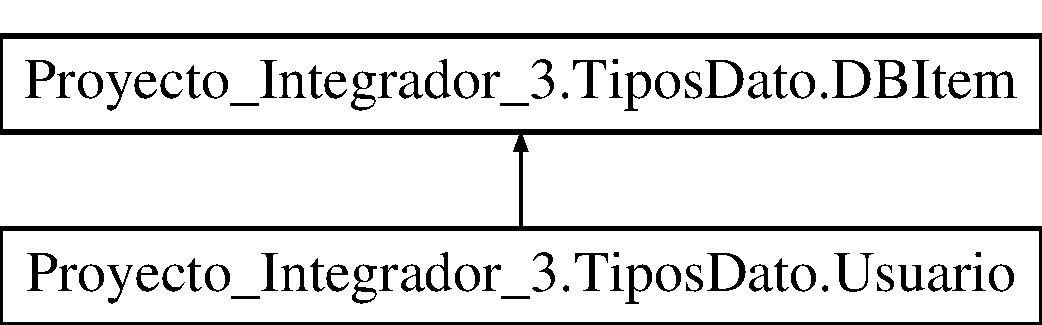
\includegraphics[height=2.000000cm]{class_proyecto___integrador__3_1_1_tipos_dato_1_1_usuario}
\end{center}
\end{figure}
\subsection*{Clases}
\begin{DoxyCompactItemize}
\item 
struct \hyperlink{struct_proyecto___integrador__3_1_1_tipos_dato_1_1_usuario_1_1_contacto}{Contacto}
\item 
struct \hyperlink{struct_proyecto___integrador__3_1_1_tipos_dato_1_1_usuario_1_1_domicilio}{Domicilio}
\end{DoxyCompactItemize}
\subsection*{Métodos públicos}
\begin{DoxyCompactItemize}
\item 
\hyperlink{class_proyecto___integrador__3_1_1_tipos_dato_1_1_usuario_a4b727b3cfd600bbecd0f5a2673152110}{Usuario} ()
\item 
override bool \hyperlink{class_proyecto___integrador__3_1_1_tipos_dato_1_1_usuario_a6ebae0d39a68af27c93fd85719bb1664}{is\-Added} ()
\begin{DoxyCompactList}\small\item\em Determina si esta instancia esta agregada a la base de datos. \end{DoxyCompactList}\item 
override string \hyperlink{class_proyecto___integrador__3_1_1_tipos_dato_1_1_usuario_ad04ec01ff1bc03efc0d4defd5589ba52}{To\-String} ()
\end{DoxyCompactItemize}
\subsection*{Atributos públicos}
\begin{DoxyCompactItemize}
\item 
bool \hyperlink{class_proyecto___integrador__3_1_1_tipos_dato_1_1_usuario_a1a0f91fb9a1e9b12a534a31295531498}{\-\_\-sexo}
\end{DoxyCompactItemize}
\subsection*{Propiedades}
\begin{DoxyCompactItemize}
\item 
Date\-Time \hyperlink{class_proyecto___integrador__3_1_1_tipos_dato_1_1_usuario_acb7c4051a5323df336c32d932b5e83bb}{Fecha\-Nacimiento}\hspace{0.3cm}{\ttfamily  \mbox{[}get, set\mbox{]}}
\item 
System.\-Guid \hyperlink{class_proyecto___integrador__3_1_1_tipos_dato_1_1_usuario_ae9cfa8c8b462028b8c166f7a1eff5f1f}{Uid}\hspace{0.3cm}{\ttfamily  \mbox{[}get, set\mbox{]}}
\item 
string \hyperlink{class_proyecto___integrador__3_1_1_tipos_dato_1_1_usuario_a22974b12ffb877b220ac230d9ce48615}{s\-Nombre}\hspace{0.3cm}{\ttfamily  \mbox{[}get\mbox{]}}
\item 
string \hyperlink{class_proyecto___integrador__3_1_1_tipos_dato_1_1_usuario_a3e82a41aeb5d99fb13d1d69ed40b1cb9}{Nombre}\hspace{0.3cm}{\ttfamily  \mbox{[}get, set\mbox{]}}
\item 
\hyperlink{struct_proyecto___integrador__3_1_1_tipos_dato_1_1_usuario_1_1_domicilio}{Domicilio} \hyperlink{class_proyecto___integrador__3_1_1_tipos_dato_1_1_usuario_aa5cabdf3a53f849c78040fc52b58d63f}{m\-Domicilio}\hspace{0.3cm}{\ttfamily  \mbox{[}get, set\mbox{]}}
\item 
string \hyperlink{class_proyecto___integrador__3_1_1_tipos_dato_1_1_usuario_a576131d83803eab74ec85992416f1220}{Telefono}\hspace{0.3cm}{\ttfamily  \mbox{[}get, set\mbox{]}}
\item 
string \hyperlink{class_proyecto___integrador__3_1_1_tipos_dato_1_1_usuario_aaf69133c2acd8387493608e39b5e4a2e}{Celular}\hspace{0.3cm}{\ttfamily  \mbox{[}get, set\mbox{]}}
\item 
int \hyperlink{class_proyecto___integrador__3_1_1_tipos_dato_1_1_usuario_a03896a1cdb77ff1166088f707b65896c}{Tipo\-Sangre}\hspace{0.3cm}{\ttfamily  \mbox{[}get, set\mbox{]}}
\item 
string \hyperlink{class_proyecto___integrador__3_1_1_tipos_dato_1_1_usuario_ab943506068326001f8581e7df6df6c14}{Alergias}\hspace{0.3cm}{\ttfamily  \mbox{[}get, set\mbox{]}}
\item 
\hyperlink{struct_proyecto___integrador__3_1_1_tipos_dato_1_1_usuario_1_1_contacto}{Contacto} \hyperlink{class_proyecto___integrador__3_1_1_tipos_dato_1_1_usuario_a2c64e3cc33009cfc51e7f68fb28024e5}{m\-Contacto}\hspace{0.3cm}{\ttfamily  \mbox{[}get, set\mbox{]}}
\item 
byte \hyperlink{class_proyecto___integrador__3_1_1_tipos_dato_1_1_usuario_a56f1e08f344ba5851703edab28232278}{Tipo\-Usuario}\hspace{0.3cm}{\ttfamily  \mbox{[}get, set\mbox{]}}
\item 
string \hyperlink{class_proyecto___integrador__3_1_1_tipos_dato_1_1_usuario_a11a9f4324ce06becd4385cdf769f5c4e}{s\-Tipo\-Usuario}\hspace{0.3cm}{\ttfamily  \mbox{[}get\mbox{]}}
\item 
decimal \hyperlink{class_proyecto___integrador__3_1_1_tipos_dato_1_1_usuario_ad29821993f63ad36d711b1e2b90b1be0}{Saldo}\hspace{0.3cm}{\ttfamily  \mbox{[}get, set\mbox{]}}
\item 
string \hyperlink{class_proyecto___integrador__3_1_1_tipos_dato_1_1_usuario_a4ecaaf4c0f0b8e78d71fcab8c7da253a}{Tarjeta\-Asignada}\hspace{0.3cm}{\ttfamily  \mbox{[}get, set\mbox{]}}
\item 
string \hyperlink{class_proyecto___integrador__3_1_1_tipos_dato_1_1_usuario_ac9a394490635d1d8083c88df4d02a84e}{Sexo}\hspace{0.3cm}{\ttfamily  \mbox{[}get, set\mbox{]}}
\item 
virtual I\-Collection$<$ \hyperlink{class_proyecto___integrador__3_1_1_tipos_dato_1_1_servicio}{Servicio} $>$ \hyperlink{class_proyecto___integrador__3_1_1_tipos_dato_1_1_usuario_a95e6bba4296f208230d6374df201f24b}{Servicios}\hspace{0.3cm}{\ttfamily  \mbox{[}get, set\mbox{]}}
\item 
virtual int \hyperlink{class_proyecto___integrador__3_1_1_tipos_dato_1_1_usuario_a28988ddc822fdf9d27d55cc2340ab65f}{Servicios\-Count}\hspace{0.3cm}{\ttfamily  \mbox{[}get\mbox{]}}
\item 
virtual Decimal \hyperlink{class_proyecto___integrador__3_1_1_tipos_dato_1_1_usuario_a17dc01f570b4c27936b81d486fc4a8bb}{Consumo}\hspace{0.3cm}{\ttfamily  \mbox{[}get\mbox{]}}
\end{DoxyCompactItemize}


\subsection{Descripción detallada}


Definición en la línea 6 del archivo Usuario.\-cs.



\subsection{Documentación del constructor y destructor}
\hypertarget{class_proyecto___integrador__3_1_1_tipos_dato_1_1_usuario_a4b727b3cfd600bbecd0f5a2673152110}{\index{Proyecto\-\_\-\-Integrador\-\_\-3\-::\-Tipos\-Dato\-::\-Usuario@{Proyecto\-\_\-\-Integrador\-\_\-3\-::\-Tipos\-Dato\-::\-Usuario}!Usuario@{Usuario}}
\index{Usuario@{Usuario}!Proyecto_Integrador_3::TiposDato::Usuario@{Proyecto\-\_\-\-Integrador\-\_\-3\-::\-Tipos\-Dato\-::\-Usuario}}
\subsubsection[{Usuario}]{\setlength{\rightskip}{0pt plus 5cm}Proyecto\-\_\-\-Integrador\-\_\-3.\-Tipos\-Dato.\-Usuario.\-Usuario (
\begin{DoxyParamCaption}
{}
\end{DoxyParamCaption}
)\hspace{0.3cm}{\ttfamily [inline]}}}\label{class_proyecto___integrador__3_1_1_tipos_dato_1_1_usuario_a4b727b3cfd600bbecd0f5a2673152110}


Definición en la línea 26 del archivo Usuario.\-cs.


\begin{DoxyCode}
27         \{
28             this.\hyperlink{class_proyecto___integrador__3_1_1_tipos_dato_1_1_usuario_a56f1e08f344ba5851703edab28232278}{TipoUsuario} = 1;
29             this.\hyperlink{class_proyecto___integrador__3_1_1_tipos_dato_1_1_usuario_ad29821993f63ad36d711b1e2b90b1be0}{Saldo} = 0;
30             this.\hyperlink{class_proyecto___integrador__3_1_1_tipos_dato_1_1_usuario_a95e6bba4296f208230d6374df201f24b}{Servicios} = \textcolor{keyword}{new} HashSet<Servicio>();
31         \}
\end{DoxyCode}


\subsection{Documentación de las funciones miembro}
\hypertarget{class_proyecto___integrador__3_1_1_tipos_dato_1_1_usuario_a6ebae0d39a68af27c93fd85719bb1664}{\index{Proyecto\-\_\-\-Integrador\-\_\-3\-::\-Tipos\-Dato\-::\-Usuario@{Proyecto\-\_\-\-Integrador\-\_\-3\-::\-Tipos\-Dato\-::\-Usuario}!is\-Added@{is\-Added}}
\index{is\-Added@{is\-Added}!Proyecto_Integrador_3::TiposDato::Usuario@{Proyecto\-\_\-\-Integrador\-\_\-3\-::\-Tipos\-Dato\-::\-Usuario}}
\subsubsection[{is\-Added}]{\setlength{\rightskip}{0pt plus 5cm}override bool Proyecto\-\_\-\-Integrador\-\_\-3.\-Tipos\-Dato.\-Usuario.\-is\-Added (
\begin{DoxyParamCaption}
{}
\end{DoxyParamCaption}
)\hspace{0.3cm}{\ttfamily [inline]}, {\ttfamily [virtual]}}}\label{class_proyecto___integrador__3_1_1_tipos_dato_1_1_usuario_a6ebae0d39a68af27c93fd85719bb1664}


Determina si esta instancia esta agregada a la base de datos. 

\begin{DoxyReturn}{Devuelve}
Verdadero si esta agregada, falso si no
\end{DoxyReturn}


Reimplementado de \hyperlink{class_proyecto___integrador__3_1_1_tipos_dato_1_1_d_b_item_ab88d7eef0fa58d7d5fdf40039867dd6e}{Proyecto\-\_\-\-Integrador\-\_\-3.\-Tipos\-Dato.\-D\-B\-Item}.



Definición en la línea 121 del archivo Usuario.\-cs.


\begin{DoxyCode}
122         \{
123             \textcolor{keywordflow}{return} !(\hyperlink{class_proyecto___integrador__3_1_1_tipos_dato_1_1_usuario_ae9cfa8c8b462028b8c166f7a1eff5f1f}{Uid} == Guid.Empty);
124         \}
\end{DoxyCode}
\hypertarget{class_proyecto___integrador__3_1_1_tipos_dato_1_1_usuario_ad04ec01ff1bc03efc0d4defd5589ba52}{\index{Proyecto\-\_\-\-Integrador\-\_\-3\-::\-Tipos\-Dato\-::\-Usuario@{Proyecto\-\_\-\-Integrador\-\_\-3\-::\-Tipos\-Dato\-::\-Usuario}!To\-String@{To\-String}}
\index{To\-String@{To\-String}!Proyecto_Integrador_3::TiposDato::Usuario@{Proyecto\-\_\-\-Integrador\-\_\-3\-::\-Tipos\-Dato\-::\-Usuario}}
\subsubsection[{To\-String}]{\setlength{\rightskip}{0pt plus 5cm}override string Proyecto\-\_\-\-Integrador\-\_\-3.\-Tipos\-Dato.\-Usuario.\-To\-String (
\begin{DoxyParamCaption}
{}
\end{DoxyParamCaption}
)\hspace{0.3cm}{\ttfamily [inline]}}}\label{class_proyecto___integrador__3_1_1_tipos_dato_1_1_usuario_ad04ec01ff1bc03efc0d4defd5589ba52}


Definición en la línea 126 del archivo Usuario.\-cs.


\begin{DoxyCode}
127         \{
128             \textcolor{keywordflow}{return} \hyperlink{class_proyecto___integrador__3_1_1_tipos_dato_1_1_usuario_a22974b12ffb877b220ac230d9ce48615}{sNombre};
129         \}
\end{DoxyCode}


\subsection{Documentación de los datos miembro}
\hypertarget{class_proyecto___integrador__3_1_1_tipos_dato_1_1_usuario_a1a0f91fb9a1e9b12a534a31295531498}{\index{Proyecto\-\_\-\-Integrador\-\_\-3\-::\-Tipos\-Dato\-::\-Usuario@{Proyecto\-\_\-\-Integrador\-\_\-3\-::\-Tipos\-Dato\-::\-Usuario}!\-\_\-sexo@{\-\_\-sexo}}
\index{\-\_\-sexo@{\-\_\-sexo}!Proyecto_Integrador_3::TiposDato::Usuario@{Proyecto\-\_\-\-Integrador\-\_\-3\-::\-Tipos\-Dato\-::\-Usuario}}
\subsubsection[{\-\_\-sexo}]{\setlength{\rightskip}{0pt plus 5cm}bool Proyecto\-\_\-\-Integrador\-\_\-3.\-Tipos\-Dato.\-Usuario.\-\_\-sexo}}\label{class_proyecto___integrador__3_1_1_tipos_dato_1_1_usuario_a1a0f91fb9a1e9b12a534a31295531498}


Definición en la línea 73 del archivo Usuario.\-cs.



\subsection{Documentación de propiedades}
\hypertarget{class_proyecto___integrador__3_1_1_tipos_dato_1_1_usuario_ab943506068326001f8581e7df6df6c14}{\index{Proyecto\-\_\-\-Integrador\-\_\-3\-::\-Tipos\-Dato\-::\-Usuario@{Proyecto\-\_\-\-Integrador\-\_\-3\-::\-Tipos\-Dato\-::\-Usuario}!Alergias@{Alergias}}
\index{Alergias@{Alergias}!Proyecto_Integrador_3::TiposDato::Usuario@{Proyecto\-\_\-\-Integrador\-\_\-3\-::\-Tipos\-Dato\-::\-Usuario}}
\subsubsection[{Alergias}]{\setlength{\rightskip}{0pt plus 5cm}string Proyecto\-\_\-\-Integrador\-\_\-3.\-Tipos\-Dato.\-Usuario.\-Alergias\hspace{0.3cm}{\ttfamily [get]}, {\ttfamily [set]}}}\label{class_proyecto___integrador__3_1_1_tipos_dato_1_1_usuario_ab943506068326001f8581e7df6df6c14}


Definición en la línea 55 del archivo Usuario.\-cs.

\hypertarget{class_proyecto___integrador__3_1_1_tipos_dato_1_1_usuario_aaf69133c2acd8387493608e39b5e4a2e}{\index{Proyecto\-\_\-\-Integrador\-\_\-3\-::\-Tipos\-Dato\-::\-Usuario@{Proyecto\-\_\-\-Integrador\-\_\-3\-::\-Tipos\-Dato\-::\-Usuario}!Celular@{Celular}}
\index{Celular@{Celular}!Proyecto_Integrador_3::TiposDato::Usuario@{Proyecto\-\_\-\-Integrador\-\_\-3\-::\-Tipos\-Dato\-::\-Usuario}}
\subsubsection[{Celular}]{\setlength{\rightskip}{0pt plus 5cm}string Proyecto\-\_\-\-Integrador\-\_\-3.\-Tipos\-Dato.\-Usuario.\-Celular\hspace{0.3cm}{\ttfamily [get]}, {\ttfamily [set]}}}\label{class_proyecto___integrador__3_1_1_tipos_dato_1_1_usuario_aaf69133c2acd8387493608e39b5e4a2e}


Definición en la línea 51 del archivo Usuario.\-cs.

\hypertarget{class_proyecto___integrador__3_1_1_tipos_dato_1_1_usuario_a17dc01f570b4c27936b81d486fc4a8bb}{\index{Proyecto\-\_\-\-Integrador\-\_\-3\-::\-Tipos\-Dato\-::\-Usuario@{Proyecto\-\_\-\-Integrador\-\_\-3\-::\-Tipos\-Dato\-::\-Usuario}!Consumo@{Consumo}}
\index{Consumo@{Consumo}!Proyecto_Integrador_3::TiposDato::Usuario@{Proyecto\-\_\-\-Integrador\-\_\-3\-::\-Tipos\-Dato\-::\-Usuario}}
\subsubsection[{Consumo}]{\setlength{\rightskip}{0pt plus 5cm}virtual Decimal Proyecto\-\_\-\-Integrador\-\_\-3.\-Tipos\-Dato.\-Usuario.\-Consumo\hspace{0.3cm}{\ttfamily [get]}}}\label{class_proyecto___integrador__3_1_1_tipos_dato_1_1_usuario_a17dc01f570b4c27936b81d486fc4a8bb}


Definición en la línea 95 del archivo Usuario.\-cs.

\hypertarget{class_proyecto___integrador__3_1_1_tipos_dato_1_1_usuario_acb7c4051a5323df336c32d932b5e83bb}{\index{Proyecto\-\_\-\-Integrador\-\_\-3\-::\-Tipos\-Dato\-::\-Usuario@{Proyecto\-\_\-\-Integrador\-\_\-3\-::\-Tipos\-Dato\-::\-Usuario}!Fecha\-Nacimiento@{Fecha\-Nacimiento}}
\index{Fecha\-Nacimiento@{Fecha\-Nacimiento}!Proyecto_Integrador_3::TiposDato::Usuario@{Proyecto\-\_\-\-Integrador\-\_\-3\-::\-Tipos\-Dato\-::\-Usuario}}
\subsubsection[{Fecha\-Nacimiento}]{\setlength{\rightskip}{0pt plus 5cm}Date\-Time Proyecto\-\_\-\-Integrador\-\_\-3.\-Tipos\-Dato.\-Usuario.\-Fecha\-Nacimiento\hspace{0.3cm}{\ttfamily [get]}, {\ttfamily [set]}}}\label{class_proyecto___integrador__3_1_1_tipos_dato_1_1_usuario_acb7c4051a5323df336c32d932b5e83bb}


Definición en la línea 33 del archivo Usuario.\-cs.

\hypertarget{class_proyecto___integrador__3_1_1_tipos_dato_1_1_usuario_a2c64e3cc33009cfc51e7f68fb28024e5}{\index{Proyecto\-\_\-\-Integrador\-\_\-3\-::\-Tipos\-Dato\-::\-Usuario@{Proyecto\-\_\-\-Integrador\-\_\-3\-::\-Tipos\-Dato\-::\-Usuario}!m\-Contacto@{m\-Contacto}}
\index{m\-Contacto@{m\-Contacto}!Proyecto_Integrador_3::TiposDato::Usuario@{Proyecto\-\_\-\-Integrador\-\_\-3\-::\-Tipos\-Dato\-::\-Usuario}}
\subsubsection[{m\-Contacto}]{\setlength{\rightskip}{0pt plus 5cm}{\bf Contacto} Proyecto\-\_\-\-Integrador\-\_\-3.\-Tipos\-Dato.\-Usuario.\-m\-Contacto\hspace{0.3cm}{\ttfamily [get]}, {\ttfamily [set]}}}\label{class_proyecto___integrador__3_1_1_tipos_dato_1_1_usuario_a2c64e3cc33009cfc51e7f68fb28024e5}


Definición en la línea 57 del archivo Usuario.\-cs.

\hypertarget{class_proyecto___integrador__3_1_1_tipos_dato_1_1_usuario_aa5cabdf3a53f849c78040fc52b58d63f}{\index{Proyecto\-\_\-\-Integrador\-\_\-3\-::\-Tipos\-Dato\-::\-Usuario@{Proyecto\-\_\-\-Integrador\-\_\-3\-::\-Tipos\-Dato\-::\-Usuario}!m\-Domicilio@{m\-Domicilio}}
\index{m\-Domicilio@{m\-Domicilio}!Proyecto_Integrador_3::TiposDato::Usuario@{Proyecto\-\_\-\-Integrador\-\_\-3\-::\-Tipos\-Dato\-::\-Usuario}}
\subsubsection[{m\-Domicilio}]{\setlength{\rightskip}{0pt plus 5cm}{\bf Domicilio} Proyecto\-\_\-\-Integrador\-\_\-3.\-Tipos\-Dato.\-Usuario.\-m\-Domicilio\hspace{0.3cm}{\ttfamily [get]}, {\ttfamily [set]}}}\label{class_proyecto___integrador__3_1_1_tipos_dato_1_1_usuario_aa5cabdf3a53f849c78040fc52b58d63f}


Definición en la línea 47 del archivo Usuario.\-cs.

\hypertarget{class_proyecto___integrador__3_1_1_tipos_dato_1_1_usuario_a3e82a41aeb5d99fb13d1d69ed40b1cb9}{\index{Proyecto\-\_\-\-Integrador\-\_\-3\-::\-Tipos\-Dato\-::\-Usuario@{Proyecto\-\_\-\-Integrador\-\_\-3\-::\-Tipos\-Dato\-::\-Usuario}!Nombre@{Nombre}}
\index{Nombre@{Nombre}!Proyecto_Integrador_3::TiposDato::Usuario@{Proyecto\-\_\-\-Integrador\-\_\-3\-::\-Tipos\-Dato\-::\-Usuario}}
\subsubsection[{Nombre}]{\setlength{\rightskip}{0pt plus 5cm}string Proyecto\-\_\-\-Integrador\-\_\-3.\-Tipos\-Dato.\-Usuario.\-Nombre\hspace{0.3cm}{\ttfamily [get]}, {\ttfamily [set]}}}\label{class_proyecto___integrador__3_1_1_tipos_dato_1_1_usuario_a3e82a41aeb5d99fb13d1d69ed40b1cb9}


Definición en la línea 45 del archivo Usuario.\-cs.

\hypertarget{class_proyecto___integrador__3_1_1_tipos_dato_1_1_usuario_ad29821993f63ad36d711b1e2b90b1be0}{\index{Proyecto\-\_\-\-Integrador\-\_\-3\-::\-Tipos\-Dato\-::\-Usuario@{Proyecto\-\_\-\-Integrador\-\_\-3\-::\-Tipos\-Dato\-::\-Usuario}!Saldo@{Saldo}}
\index{Saldo@{Saldo}!Proyecto_Integrador_3::TiposDato::Usuario@{Proyecto\-\_\-\-Integrador\-\_\-3\-::\-Tipos\-Dato\-::\-Usuario}}
\subsubsection[{Saldo}]{\setlength{\rightskip}{0pt plus 5cm}decimal Proyecto\-\_\-\-Integrador\-\_\-3.\-Tipos\-Dato.\-Usuario.\-Saldo\hspace{0.3cm}{\ttfamily [get]}, {\ttfamily [set]}}}\label{class_proyecto___integrador__3_1_1_tipos_dato_1_1_usuario_ad29821993f63ad36d711b1e2b90b1be0}


Definición en la línea 69 del archivo Usuario.\-cs.

\hypertarget{class_proyecto___integrador__3_1_1_tipos_dato_1_1_usuario_a95e6bba4296f208230d6374df201f24b}{\index{Proyecto\-\_\-\-Integrador\-\_\-3\-::\-Tipos\-Dato\-::\-Usuario@{Proyecto\-\_\-\-Integrador\-\_\-3\-::\-Tipos\-Dato\-::\-Usuario}!Servicios@{Servicios}}
\index{Servicios@{Servicios}!Proyecto_Integrador_3::TiposDato::Usuario@{Proyecto\-\_\-\-Integrador\-\_\-3\-::\-Tipos\-Dato\-::\-Usuario}}
\subsubsection[{Servicios}]{\setlength{\rightskip}{0pt plus 5cm}virtual I\-Collection$<${\bf Servicio}$>$ Proyecto\-\_\-\-Integrador\-\_\-3.\-Tipos\-Dato.\-Usuario.\-Servicios\hspace{0.3cm}{\ttfamily [get]}, {\ttfamily [set]}}}\label{class_proyecto___integrador__3_1_1_tipos_dato_1_1_usuario_a95e6bba4296f208230d6374df201f24b}


Definición en la línea 77 del archivo Usuario.\-cs.

\hypertarget{class_proyecto___integrador__3_1_1_tipos_dato_1_1_usuario_a28988ddc822fdf9d27d55cc2340ab65f}{\index{Proyecto\-\_\-\-Integrador\-\_\-3\-::\-Tipos\-Dato\-::\-Usuario@{Proyecto\-\_\-\-Integrador\-\_\-3\-::\-Tipos\-Dato\-::\-Usuario}!Servicios\-Count@{Servicios\-Count}}
\index{Servicios\-Count@{Servicios\-Count}!Proyecto_Integrador_3::TiposDato::Usuario@{Proyecto\-\_\-\-Integrador\-\_\-3\-::\-Tipos\-Dato\-::\-Usuario}}
\subsubsection[{Servicios\-Count}]{\setlength{\rightskip}{0pt plus 5cm}virtual int Proyecto\-\_\-\-Integrador\-\_\-3.\-Tipos\-Dato.\-Usuario.\-Servicios\-Count\hspace{0.3cm}{\ttfamily [get]}}}\label{class_proyecto___integrador__3_1_1_tipos_dato_1_1_usuario_a28988ddc822fdf9d27d55cc2340ab65f}


Definición en la línea 80 del archivo Usuario.\-cs.

\hypertarget{class_proyecto___integrador__3_1_1_tipos_dato_1_1_usuario_ac9a394490635d1d8083c88df4d02a84e}{\index{Proyecto\-\_\-\-Integrador\-\_\-3\-::\-Tipos\-Dato\-::\-Usuario@{Proyecto\-\_\-\-Integrador\-\_\-3\-::\-Tipos\-Dato\-::\-Usuario}!Sexo@{Sexo}}
\index{Sexo@{Sexo}!Proyecto_Integrador_3::TiposDato::Usuario@{Proyecto\-\_\-\-Integrador\-\_\-3\-::\-Tipos\-Dato\-::\-Usuario}}
\subsubsection[{Sexo}]{\setlength{\rightskip}{0pt plus 5cm}string Proyecto\-\_\-\-Integrador\-\_\-3.\-Tipos\-Dato.\-Usuario.\-Sexo\hspace{0.3cm}{\ttfamily [get]}, {\ttfamily [set]}}}\label{class_proyecto___integrador__3_1_1_tipos_dato_1_1_usuario_ac9a394490635d1d8083c88df4d02a84e}


Definición en la línea 75 del archivo Usuario.\-cs.

\hypertarget{class_proyecto___integrador__3_1_1_tipos_dato_1_1_usuario_a22974b12ffb877b220ac230d9ce48615}{\index{Proyecto\-\_\-\-Integrador\-\_\-3\-::\-Tipos\-Dato\-::\-Usuario@{Proyecto\-\_\-\-Integrador\-\_\-3\-::\-Tipos\-Dato\-::\-Usuario}!s\-Nombre@{s\-Nombre}}
\index{s\-Nombre@{s\-Nombre}!Proyecto_Integrador_3::TiposDato::Usuario@{Proyecto\-\_\-\-Integrador\-\_\-3\-::\-Tipos\-Dato\-::\-Usuario}}
\subsubsection[{s\-Nombre}]{\setlength{\rightskip}{0pt plus 5cm}string Proyecto\-\_\-\-Integrador\-\_\-3.\-Tipos\-Dato.\-Usuario.\-s\-Nombre\hspace{0.3cm}{\ttfamily [get]}}}\label{class_proyecto___integrador__3_1_1_tipos_dato_1_1_usuario_a22974b12ffb877b220ac230d9ce48615}


Definición en la línea 38 del archivo Usuario.\-cs.

\hypertarget{class_proyecto___integrador__3_1_1_tipos_dato_1_1_usuario_a11a9f4324ce06becd4385cdf769f5c4e}{\index{Proyecto\-\_\-\-Integrador\-\_\-3\-::\-Tipos\-Dato\-::\-Usuario@{Proyecto\-\_\-\-Integrador\-\_\-3\-::\-Tipos\-Dato\-::\-Usuario}!s\-Tipo\-Usuario@{s\-Tipo\-Usuario}}
\index{s\-Tipo\-Usuario@{s\-Tipo\-Usuario}!Proyecto_Integrador_3::TiposDato::Usuario@{Proyecto\-\_\-\-Integrador\-\_\-3\-::\-Tipos\-Dato\-::\-Usuario}}
\subsubsection[{s\-Tipo\-Usuario}]{\setlength{\rightskip}{0pt plus 5cm}string Proyecto\-\_\-\-Integrador\-\_\-3.\-Tipos\-Dato.\-Usuario.\-s\-Tipo\-Usuario\hspace{0.3cm}{\ttfamily [get]}}}\label{class_proyecto___integrador__3_1_1_tipos_dato_1_1_usuario_a11a9f4324ce06becd4385cdf769f5c4e}


Definición en la línea 62 del archivo Usuario.\-cs.

\hypertarget{class_proyecto___integrador__3_1_1_tipos_dato_1_1_usuario_a4ecaaf4c0f0b8e78d71fcab8c7da253a}{\index{Proyecto\-\_\-\-Integrador\-\_\-3\-::\-Tipos\-Dato\-::\-Usuario@{Proyecto\-\_\-\-Integrador\-\_\-3\-::\-Tipos\-Dato\-::\-Usuario}!Tarjeta\-Asignada@{Tarjeta\-Asignada}}
\index{Tarjeta\-Asignada@{Tarjeta\-Asignada}!Proyecto_Integrador_3::TiposDato::Usuario@{Proyecto\-\_\-\-Integrador\-\_\-3\-::\-Tipos\-Dato\-::\-Usuario}}
\subsubsection[{Tarjeta\-Asignada}]{\setlength{\rightskip}{0pt plus 5cm}string Proyecto\-\_\-\-Integrador\-\_\-3.\-Tipos\-Dato.\-Usuario.\-Tarjeta\-Asignada\hspace{0.3cm}{\ttfamily [get]}, {\ttfamily [set]}}}\label{class_proyecto___integrador__3_1_1_tipos_dato_1_1_usuario_a4ecaaf4c0f0b8e78d71fcab8c7da253a}


Definición en la línea 71 del archivo Usuario.\-cs.

\hypertarget{class_proyecto___integrador__3_1_1_tipos_dato_1_1_usuario_a576131d83803eab74ec85992416f1220}{\index{Proyecto\-\_\-\-Integrador\-\_\-3\-::\-Tipos\-Dato\-::\-Usuario@{Proyecto\-\_\-\-Integrador\-\_\-3\-::\-Tipos\-Dato\-::\-Usuario}!Telefono@{Telefono}}
\index{Telefono@{Telefono}!Proyecto_Integrador_3::TiposDato::Usuario@{Proyecto\-\_\-\-Integrador\-\_\-3\-::\-Tipos\-Dato\-::\-Usuario}}
\subsubsection[{Telefono}]{\setlength{\rightskip}{0pt plus 5cm}string Proyecto\-\_\-\-Integrador\-\_\-3.\-Tipos\-Dato.\-Usuario.\-Telefono\hspace{0.3cm}{\ttfamily [get]}, {\ttfamily [set]}}}\label{class_proyecto___integrador__3_1_1_tipos_dato_1_1_usuario_a576131d83803eab74ec85992416f1220}


Definición en la línea 49 del archivo Usuario.\-cs.

\hypertarget{class_proyecto___integrador__3_1_1_tipos_dato_1_1_usuario_a03896a1cdb77ff1166088f707b65896c}{\index{Proyecto\-\_\-\-Integrador\-\_\-3\-::\-Tipos\-Dato\-::\-Usuario@{Proyecto\-\_\-\-Integrador\-\_\-3\-::\-Tipos\-Dato\-::\-Usuario}!Tipo\-Sangre@{Tipo\-Sangre}}
\index{Tipo\-Sangre@{Tipo\-Sangre}!Proyecto_Integrador_3::TiposDato::Usuario@{Proyecto\-\_\-\-Integrador\-\_\-3\-::\-Tipos\-Dato\-::\-Usuario}}
\subsubsection[{Tipo\-Sangre}]{\setlength{\rightskip}{0pt plus 5cm}int Proyecto\-\_\-\-Integrador\-\_\-3.\-Tipos\-Dato.\-Usuario.\-Tipo\-Sangre\hspace{0.3cm}{\ttfamily [get]}, {\ttfamily [set]}}}\label{class_proyecto___integrador__3_1_1_tipos_dato_1_1_usuario_a03896a1cdb77ff1166088f707b65896c}


Definición en la línea 53 del archivo Usuario.\-cs.

\hypertarget{class_proyecto___integrador__3_1_1_tipos_dato_1_1_usuario_a56f1e08f344ba5851703edab28232278}{\index{Proyecto\-\_\-\-Integrador\-\_\-3\-::\-Tipos\-Dato\-::\-Usuario@{Proyecto\-\_\-\-Integrador\-\_\-3\-::\-Tipos\-Dato\-::\-Usuario}!Tipo\-Usuario@{Tipo\-Usuario}}
\index{Tipo\-Usuario@{Tipo\-Usuario}!Proyecto_Integrador_3::TiposDato::Usuario@{Proyecto\-\_\-\-Integrador\-\_\-3\-::\-Tipos\-Dato\-::\-Usuario}}
\subsubsection[{Tipo\-Usuario}]{\setlength{\rightskip}{0pt plus 5cm}byte Proyecto\-\_\-\-Integrador\-\_\-3.\-Tipos\-Dato.\-Usuario.\-Tipo\-Usuario\hspace{0.3cm}{\ttfamily [get]}, {\ttfamily [set]}}}\label{class_proyecto___integrador__3_1_1_tipos_dato_1_1_usuario_a56f1e08f344ba5851703edab28232278}


Definición en la línea 59 del archivo Usuario.\-cs.

\hypertarget{class_proyecto___integrador__3_1_1_tipos_dato_1_1_usuario_ae9cfa8c8b462028b8c166f7a1eff5f1f}{\index{Proyecto\-\_\-\-Integrador\-\_\-3\-::\-Tipos\-Dato\-::\-Usuario@{Proyecto\-\_\-\-Integrador\-\_\-3\-::\-Tipos\-Dato\-::\-Usuario}!Uid@{Uid}}
\index{Uid@{Uid}!Proyecto_Integrador_3::TiposDato::Usuario@{Proyecto\-\_\-\-Integrador\-\_\-3\-::\-Tipos\-Dato\-::\-Usuario}}
\subsubsection[{Uid}]{\setlength{\rightskip}{0pt plus 5cm}System.\-Guid Proyecto\-\_\-\-Integrador\-\_\-3.\-Tipos\-Dato.\-Usuario.\-Uid\hspace{0.3cm}{\ttfamily [get]}, {\ttfamily [set]}}}\label{class_proyecto___integrador__3_1_1_tipos_dato_1_1_usuario_ae9cfa8c8b462028b8c166f7a1eff5f1f}


Definición en la línea 35 del archivo Usuario.\-cs.



La documentación para esta clase fue generada a partir del siguiente fichero\-:\begin{DoxyCompactItemize}
\item 
C\-:/\-Users/\-Yknx4/\-Documents/\-Visual Studio 2012/\-Projects/\-Proyecto Integrador 3/\-Proyecto Integrador 3/\-Tipos\-Dato/\hyperlink{_usuario_8cs}{Usuario.\-cs}\end{DoxyCompactItemize}

\hypertarget{class_proyecto___integrador__3_1_1_d_b_managers_1_1_usuario_d_b_manager}{\section{Referencia de la Clase Proyecto\-\_\-\-Integrador\-\_\-3.\-D\-B\-Managers.\-Usuario\-D\-B\-Manager}
\label{class_proyecto___integrador__3_1_1_d_b_managers_1_1_usuario_d_b_manager}\index{Proyecto\-\_\-\-Integrador\-\_\-3.\-D\-B\-Managers.\-Usuario\-D\-B\-Manager@{Proyecto\-\_\-\-Integrador\-\_\-3.\-D\-B\-Managers.\-Usuario\-D\-B\-Manager}}
}
Diagrama de herencias de Proyecto\-\_\-\-Integrador\-\_\-3.\-D\-B\-Managers.\-Usuario\-D\-B\-Manager\begin{figure}[H]
\begin{center}
\leavevmode
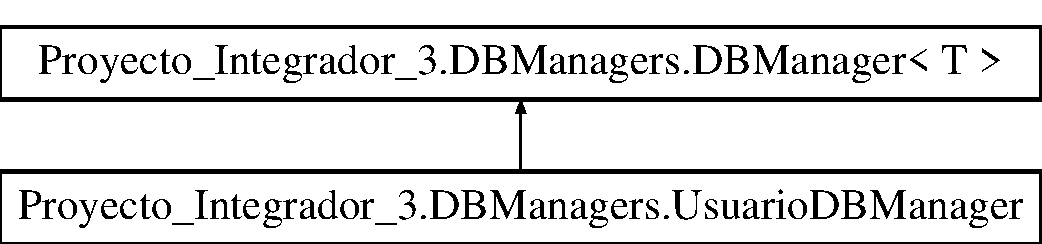
\includegraphics[height=2.000000cm]{class_proyecto___integrador__3_1_1_d_b_managers_1_1_usuario_d_b_manager}
\end{center}
\end{figure}
\subsection*{Métodos públicos}
\begin{DoxyCompactItemize}
\item 
\hyperlink{class_proyecto___integrador__3_1_1_d_b_managers_1_1_usuario_d_b_manager_a3bcff5c7839e9e78baaab699a68af438}{Usuario\-D\-B\-Manager} (\hyperlink{class_proyecto___integrador__3_1_1_d_b_managers}{D\-B\-Managers} sender)
\item 
override void \hyperlink{class_proyecto___integrador__3_1_1_d_b_managers_1_1_usuario_d_b_manager_a40976ea1cf23f128217f7379f175d504}{Add\-To\-D\-B} ()
\item 
void \hyperlink{class_proyecto___integrador__3_1_1_d_b_managers_1_1_usuario_d_b_manager_ac7fd33ab64b2c21ad0533c59eb77d118}{Add\-To\-D\-B} (Guid Uid)
\item 
\hyperlink{class_proyecto___integrador__3_1_1_tipos_dato_1_1_usuario}{Usuario} \hyperlink{class_proyecto___integrador__3_1_1_d_b_managers_1_1_usuario_d_b_manager_a4d3bacd63b66ffb89ff6f26156520072}{get\-Item} ()
\item 
override void \hyperlink{class_proyecto___integrador__3_1_1_d_b_managers_1_1_usuario_d_b_manager_a54c2d949592f354143fa7b7429ce1938}{Add\-To\-Dataset} ()
\item 
override void \hyperlink{class_proyecto___integrador__3_1_1_d_b_managers_1_1_usuario_d_b_manager_af38f312f9fd5a10d9a8d7d43e880d555}{Update\-D\-B\-From\-Dataset} ()
\item 
void \hyperlink{class_proyecto___integrador__3_1_1_d_b_managers_1_1_usuario_d_b_manager_a2aa56cfd9be44c7c601b1983e63bd6d6}{Refresh} ()
\item 
override void \hyperlink{class_proyecto___integrador__3_1_1_d_b_managers_1_1_usuario_d_b_manager_a3497931d99dff8f67c2da21b1328de1c}{item\-Modified} (object sender, Property\-Changed\-Event\-Args e)
\item 
override void \hyperlink{class_proyecto___integrador__3_1_1_d_b_managers_1_1_usuario_d_b_manager_a367d61aaac1f426d93800be80159eadd}{modificar\-Dato} ()
\item 
virtual void \hyperlink{class_proyecto___integrador__3_1_1_d_b_managers_1_1_d_b_manager_3_01_t_01_4_a49ea2a7bfa58a2c536fefa4d60d488d2}{item\-Modified} (object sender, System.\-Component\-Model.\-Property\-Changed\-Event\-Args e)
\item 
virtual bool \hyperlink{class_proyecto___integrador__3_1_1_d_b_managers_1_1_d_b_manager_3_01_t_01_4_a436cb08914ca84122f9019a59485589a}{Remove\-From\-D\-B} ()
\item 
void \hyperlink{class_proyecto___integrador__3_1_1_d_b_managers_1_1_d_b_manager_3_01_t_01_4_a2d552a5e547efd19924ca4a96f685a56}{set\-Item} (T Input)
\item 
void \hyperlink{class_proyecto___integrador__3_1_1_d_b_managers_1_1_d_b_manager_3_01_t_01_4_ad5d7f99a4a5783514bad64ba8894e1ea}{Clear} ()
\end{DoxyCompactItemize}
\subsection*{Métodos protegidos}
\begin{DoxyCompactItemize}
\item 
bool \hyperlink{class_proyecto___integrador__3_1_1_d_b_managers_1_1_d_b_manager_3_01_t_01_4_add66e324cef43fd10b491bc697fa60b5}{Active} ()
\end{DoxyCompactItemize}
\subsection*{Atributos protegidos}
\begin{DoxyCompactItemize}
\item 
\hyperlink{class_proyecto___integrador__3_1_1_d_b_managers}{D\-B\-Managers} \hyperlink{class_proyecto___integrador__3_1_1_d_b_managers_1_1_d_b_manager_3_01_t_01_4_a06315e75298c8f2fd46f32dc7c9a80b2}{Parent}
\item 
T \hyperlink{class_proyecto___integrador__3_1_1_d_b_managers_1_1_d_b_manager_3_01_t_01_4_a3b67ae3b5b3b9c3793d56c1407d7dcff}{held\-Item}
\end{DoxyCompactItemize}
\subsection*{Propiedades}
\begin{DoxyCompactItemize}
\item 
string \hyperlink{class_proyecto___integrador__3_1_1_d_b_managers_1_1_d_b_manager_3_01_t_01_4_a6e5caaed2ee1a4d067dfbf5aaa1b1fa8}{Error}\hspace{0.3cm}{\ttfamily  \mbox{[}get, set\mbox{]}}
\end{DoxyCompactItemize}
\subsection*{Métodos privados}
\begin{DoxyCompactItemize}
\item 
void \hyperlink{class_proyecto___integrador__3_1_1_d_b_managers_1_1_usuario_d_b_manager_a6d2db3445fc5acc8a349b76029714a96}{notify\-Error} ()
\item 
\hyperlink{class_proyecto___integrador__3_1_1ds_usuarios_1_1_usuarios_row}{ds\-Usuarios.\-Usuarios\-Row} \hyperlink{class_proyecto___integrador__3_1_1_d_b_managers_1_1_usuario_d_b_manager_a4e531d5e782e81b5a70ce977fef09cf4}{get\-Usuario\-Row} ()
\end{DoxyCompactItemize}


\subsection{Descripción detallada}


Definición en la línea 13 del archivo Usuario\-D\-B\-Manager.\-cs.



\subsection{Documentación del constructor y destructor}
\hypertarget{class_proyecto___integrador__3_1_1_d_b_managers_1_1_usuario_d_b_manager_a3bcff5c7839e9e78baaab699a68af438}{\index{Proyecto\-\_\-\-Integrador\-\_\-3\-::\-D\-B\-Managers\-::\-Usuario\-D\-B\-Manager@{Proyecto\-\_\-\-Integrador\-\_\-3\-::\-D\-B\-Managers\-::\-Usuario\-D\-B\-Manager}!Usuario\-D\-B\-Manager@{Usuario\-D\-B\-Manager}}
\index{Usuario\-D\-B\-Manager@{Usuario\-D\-B\-Manager}!Proyecto_Integrador_3::DBManagers::UsuarioDBManager@{Proyecto\-\_\-\-Integrador\-\_\-3\-::\-D\-B\-Managers\-::\-Usuario\-D\-B\-Manager}}
\subsubsection[{Usuario\-D\-B\-Manager}]{\setlength{\rightskip}{0pt plus 5cm}Proyecto\-\_\-\-Integrador\-\_\-3.\-D\-B\-Managers.\-Usuario\-D\-B\-Manager.\-Usuario\-D\-B\-Manager (
\begin{DoxyParamCaption}
\item[{{\bf D\-B\-Managers}}]{sender}
\end{DoxyParamCaption}
)\hspace{0.3cm}{\ttfamily [inline]}}}\label{class_proyecto___integrador__3_1_1_d_b_managers_1_1_usuario_d_b_manager_a3bcff5c7839e9e78baaab699a68af438}


Definición en la línea 15 del archivo Usuario\-D\-B\-Manager.\-cs.


\begin{DoxyCode}
16                 : base(sender)
17             \{
18             \}
\end{DoxyCode}


\subsection{Documentación de las funciones miembro}
\hypertarget{class_proyecto___integrador__3_1_1_d_b_managers_1_1_d_b_manager_3_01_t_01_4_add66e324cef43fd10b491bc697fa60b5}{\index{Proyecto\-\_\-\-Integrador\-\_\-3\-::\-D\-B\-Managers\-::\-Usuario\-D\-B\-Manager@{Proyecto\-\_\-\-Integrador\-\_\-3\-::\-D\-B\-Managers\-::\-Usuario\-D\-B\-Manager}!Active@{Active}}
\index{Active@{Active}!Proyecto_Integrador_3::DBManagers::UsuarioDBManager@{Proyecto\-\_\-\-Integrador\-\_\-3\-::\-D\-B\-Managers\-::\-Usuario\-D\-B\-Manager}}
\subsubsection[{Active}]{\setlength{\rightskip}{0pt plus 5cm}bool Proyecto\-\_\-\-Integrador\-\_\-3.\-D\-B\-Managers.\-D\-B\-Manager$<$ T $>$.Active (
\begin{DoxyParamCaption}
{}
\end{DoxyParamCaption}
)\hspace{0.3cm}{\ttfamily [inline]}, {\ttfamily [protected]}, {\ttfamily [inherited]}}}\label{class_proyecto___integrador__3_1_1_d_b_managers_1_1_d_b_manager_3_01_t_01_4_add66e324cef43fd10b491bc697fa60b5}


Definición en la línea 48 del archivo D\-B\-Manager.\-cs.


\begin{DoxyCode}
49             \{
50                 \textcolor{keywordflow}{if} (\hyperlink{class_proyecto___integrador__3_1_1_d_b_managers_1_1_d_b_manager_3_01_t_01_4_a3b67ae3b5b3b9c3793d56c1407d7dcff}{heldItem} == null) \textcolor{keywordflow}{return} \textcolor{keyword}{false};
51                 \textcolor{keywordflow}{return} \textcolor{keyword}{true};
52             \}
\end{DoxyCode}
\hypertarget{class_proyecto___integrador__3_1_1_d_b_managers_1_1_usuario_d_b_manager_a54c2d949592f354143fa7b7429ce1938}{\index{Proyecto\-\_\-\-Integrador\-\_\-3\-::\-D\-B\-Managers\-::\-Usuario\-D\-B\-Manager@{Proyecto\-\_\-\-Integrador\-\_\-3\-::\-D\-B\-Managers\-::\-Usuario\-D\-B\-Manager}!Add\-To\-Dataset@{Add\-To\-Dataset}}
\index{Add\-To\-Dataset@{Add\-To\-Dataset}!Proyecto_Integrador_3::DBManagers::UsuarioDBManager@{Proyecto\-\_\-\-Integrador\-\_\-3\-::\-D\-B\-Managers\-::\-Usuario\-D\-B\-Manager}}
\subsubsection[{Add\-To\-Dataset}]{\setlength{\rightskip}{0pt plus 5cm}override void Proyecto\-\_\-\-Integrador\-\_\-3.\-D\-B\-Managers.\-Usuario\-D\-B\-Manager.\-Add\-To\-Dataset (
\begin{DoxyParamCaption}
{}
\end{DoxyParamCaption}
)\hspace{0.3cm}{\ttfamily [inline]}, {\ttfamily [virtual]}}}\label{class_proyecto___integrador__3_1_1_d_b_managers_1_1_usuario_d_b_manager_a54c2d949592f354143fa7b7429ce1938}


Implementa \hyperlink{class_proyecto___integrador__3_1_1_d_b_managers_1_1_d_b_manager_3_01_t_01_4_a7830332e065723c1799d5804fd202dd1}{Proyecto\-\_\-\-Integrador\-\_\-3.\-D\-B\-Managers.\-D\-B\-Manager$<$ T $>$}.



Definición en la línea 48 del archivo Usuario\-D\-B\-Manager.\-cs.


\begin{DoxyCode}
49             \{
50                 \textcolor{keywordflow}{if} (!\hyperlink{class_proyecto___integrador__3_1_1_d_b_managers_1_1_d_b_manager_3_01_t_01_4_add66e324cef43fd10b491bc697fa60b5}{Active}())
51                 \{
52                     \hyperlink{class_proyecto___integrador__3_1_1_d_b_managers_1_1_d_b_manager_3_01_t_01_4_a6e5caaed2ee1a4d067dfbf5aaa1b1fa8}{Error} = \textcolor{stringliteral}{"No hay ningun usuario seleccionado"};
53                     \hyperlink{class_proyecto___integrador__3_1_1_d_b_managers_1_1_usuario_d_b_manager_a6d2db3445fc5acc8a349b76029714a96}{notifyError}();
54                 \}
55                 \hyperlink{class_proyecto___integrador__3_1_1_d_b_managers_1_1_d_b_manager_3_01_t_01_4_a3b67ae3b5b3b9c3793d56c1407d7dcff}{heldItem}.Saldo = 0;
56                 dsUsuarios.UsuariosRow nuevoUsuario = \hyperlink{class_proyecto___integrador__3_1_1_d_b_managers_1_1_usuario_d_b_manager_a4e531d5e782e81b5a70ce977fef09cf4}{getUsuarioRow}();
57                 \hyperlink{class_proyecto___integrador__3_1_1_d_b_managers_1_1_d_b_manager_3_01_t_01_4_a06315e75298c8f2fd46f32dc7c9a80b2}{Parent}.\hyperlink{class_proyecto___integrador__3_1_1_d_b_managers_a19d87c9abf32e08e2969847a008eb195}{mdsUsuarios}.\hyperlink{class_proyecto___integrador__3_1_1ds_usuarios_a79d1cfd31914c2c5cfda39b62381478b}{Usuarios}.
      \hyperlink{class_proyecto___integrador__3_1_1ds_usuarios_1_1_usuarios_data_table_a5ef8027791b5ae1564a0dce426b8f135}{AddUsuariosRow}(nuevoUsuario);
58             \}
\end{DoxyCode}
\hypertarget{class_proyecto___integrador__3_1_1_d_b_managers_1_1_usuario_d_b_manager_a40976ea1cf23f128217f7379f175d504}{\index{Proyecto\-\_\-\-Integrador\-\_\-3\-::\-D\-B\-Managers\-::\-Usuario\-D\-B\-Manager@{Proyecto\-\_\-\-Integrador\-\_\-3\-::\-D\-B\-Managers\-::\-Usuario\-D\-B\-Manager}!Add\-To\-D\-B@{Add\-To\-D\-B}}
\index{Add\-To\-D\-B@{Add\-To\-D\-B}!Proyecto_Integrador_3::DBManagers::UsuarioDBManager@{Proyecto\-\_\-\-Integrador\-\_\-3\-::\-D\-B\-Managers\-::\-Usuario\-D\-B\-Manager}}
\subsubsection[{Add\-To\-D\-B}]{\setlength{\rightskip}{0pt plus 5cm}override void Proyecto\-\_\-\-Integrador\-\_\-3.\-D\-B\-Managers.\-Usuario\-D\-B\-Manager.\-Add\-To\-D\-B (
\begin{DoxyParamCaption}
{}
\end{DoxyParamCaption}
)\hspace{0.3cm}{\ttfamily [inline]}, {\ttfamily [virtual]}}}\label{class_proyecto___integrador__3_1_1_d_b_managers_1_1_usuario_d_b_manager_a40976ea1cf23f128217f7379f175d504}


Implementa \hyperlink{class_proyecto___integrador__3_1_1_d_b_managers_1_1_d_b_manager_3_01_t_01_4_a820a55f3ee3c7fde31b121f3f3ea6179}{Proyecto\-\_\-\-Integrador\-\_\-3.\-D\-B\-Managers.\-D\-B\-Manager$<$ T $>$}.



Definición en la línea 25 del archivo Usuario\-D\-B\-Manager.\-cs.


\begin{DoxyCode}
26             \{
27                 \textcolor{keywordflow}{if} (\hyperlink{class_proyecto___integrador__3_1_1_d_b_managers_1_1_d_b_manager_3_01_t_01_4_a3b67ae3b5b3b9c3793d56c1407d7dcff}{heldItem}.isAdded())
28                 \{
29                     \hyperlink{class_proyecto___integrador__3_1_1_d_b_managers_1_1_d_b_manager_3_01_t_01_4_a6e5caaed2ee1a4d067dfbf5aaa1b1fa8}{Error} = \textcolor{stringliteral}{"El usuario con ID "} + \hyperlink{class_proyecto___integrador__3_1_1_d_b_managers_1_1_d_b_manager_3_01_t_01_4_a3b67ae3b5b3b9c3793d56c1407d7dcff}{heldItem}.Uid.ToString() + \textcolor{stringliteral}{" ya está en la
       base de datos"};
30                     \hyperlink{class_proyecto___integrador__3_1_1_d_b_managers_1_1_usuario_d_b_manager_a6d2db3445fc5acc8a349b76029714a96}{notifyError}();
31                 \}
32 
33                 \hyperlink{class_proyecto___integrador__3_1_1_d_b_managers_1_1_usuario_d_b_manager_a40976ea1cf23f128217f7379f175d504}{AddToDB}(Guid.NewGuid());
34             \}
\end{DoxyCode}
\hypertarget{class_proyecto___integrador__3_1_1_d_b_managers_1_1_usuario_d_b_manager_ac7fd33ab64b2c21ad0533c59eb77d118}{\index{Proyecto\-\_\-\-Integrador\-\_\-3\-::\-D\-B\-Managers\-::\-Usuario\-D\-B\-Manager@{Proyecto\-\_\-\-Integrador\-\_\-3\-::\-D\-B\-Managers\-::\-Usuario\-D\-B\-Manager}!Add\-To\-D\-B@{Add\-To\-D\-B}}
\index{Add\-To\-D\-B@{Add\-To\-D\-B}!Proyecto_Integrador_3::DBManagers::UsuarioDBManager@{Proyecto\-\_\-\-Integrador\-\_\-3\-::\-D\-B\-Managers\-::\-Usuario\-D\-B\-Manager}}
\subsubsection[{Add\-To\-D\-B}]{\setlength{\rightskip}{0pt plus 5cm}void Proyecto\-\_\-\-Integrador\-\_\-3.\-D\-B\-Managers.\-Usuario\-D\-B\-Manager.\-Add\-To\-D\-B (
\begin{DoxyParamCaption}
\item[{Guid}]{Uid}
\end{DoxyParamCaption}
)\hspace{0.3cm}{\ttfamily [inline]}}}\label{class_proyecto___integrador__3_1_1_d_b_managers_1_1_usuario_d_b_manager_ac7fd33ab64b2c21ad0533c59eb77d118}


Definición en la línea 36 del archivo Usuario\-D\-B\-Manager.\-cs.


\begin{DoxyCode}
37             \{
38                 \hyperlink{class_proyecto___integrador__3_1_1_d_b_managers_1_1_d_b_manager_3_01_t_01_4_a3b67ae3b5b3b9c3793d56c1407d7dcff}{heldItem}.Uid = Uid;
39                 \hyperlink{class_proyecto___integrador__3_1_1_d_b_managers_1_1_usuario_d_b_manager_a54c2d949592f354143fa7b7429ce1938}{AddToDataset}();
40                 \hyperlink{class_proyecto___integrador__3_1_1_d_b_managers_1_1_usuario_d_b_manager_af38f312f9fd5a10d9a8d7d43e880d555}{UpdateDBFromDataset}();
41             \}
\end{DoxyCode}
\hypertarget{class_proyecto___integrador__3_1_1_d_b_managers_1_1_d_b_manager_3_01_t_01_4_ad5d7f99a4a5783514bad64ba8894e1ea}{\index{Proyecto\-\_\-\-Integrador\-\_\-3\-::\-D\-B\-Managers\-::\-Usuario\-D\-B\-Manager@{Proyecto\-\_\-\-Integrador\-\_\-3\-::\-D\-B\-Managers\-::\-Usuario\-D\-B\-Manager}!Clear@{Clear}}
\index{Clear@{Clear}!Proyecto_Integrador_3::DBManagers::UsuarioDBManager@{Proyecto\-\_\-\-Integrador\-\_\-3\-::\-D\-B\-Managers\-::\-Usuario\-D\-B\-Manager}}
\subsubsection[{Clear}]{\setlength{\rightskip}{0pt plus 5cm}void Proyecto\-\_\-\-Integrador\-\_\-3.\-D\-B\-Managers.\-D\-B\-Manager$<$ T $>$.Clear (
\begin{DoxyParamCaption}
{}
\end{DoxyParamCaption}
)\hspace{0.3cm}{\ttfamily [inline]}, {\ttfamily [inherited]}}}\label{class_proyecto___integrador__3_1_1_d_b_managers_1_1_d_b_manager_3_01_t_01_4_ad5d7f99a4a5783514bad64ba8894e1ea}


Definición en la línea 43 del archivo D\-B\-Manager.\-cs.


\begin{DoxyCode}
44             \{
45                 \hyperlink{class_proyecto___integrador__3_1_1_d_b_managers_1_1_d_b_manager_3_01_t_01_4_a3b67ae3b5b3b9c3793d56c1407d7dcff}{heldItem} = \textcolor{keywordflow}{default}(T);
46             \}
\end{DoxyCode}
\hypertarget{class_proyecto___integrador__3_1_1_d_b_managers_1_1_usuario_d_b_manager_a4d3bacd63b66ffb89ff6f26156520072}{\index{Proyecto\-\_\-\-Integrador\-\_\-3\-::\-D\-B\-Managers\-::\-Usuario\-D\-B\-Manager@{Proyecto\-\_\-\-Integrador\-\_\-3\-::\-D\-B\-Managers\-::\-Usuario\-D\-B\-Manager}!get\-Item@{get\-Item}}
\index{get\-Item@{get\-Item}!Proyecto_Integrador_3::DBManagers::UsuarioDBManager@{Proyecto\-\_\-\-Integrador\-\_\-3\-::\-D\-B\-Managers\-::\-Usuario\-D\-B\-Manager}}
\subsubsection[{get\-Item}]{\setlength{\rightskip}{0pt plus 5cm}{\bf Usuario} Proyecto\-\_\-\-Integrador\-\_\-3.\-D\-B\-Managers.\-Usuario\-D\-B\-Manager.\-get\-Item (
\begin{DoxyParamCaption}
{}
\end{DoxyParamCaption}
)\hspace{0.3cm}{\ttfamily [inline]}}}\label{class_proyecto___integrador__3_1_1_d_b_managers_1_1_usuario_d_b_manager_a4d3bacd63b66ffb89ff6f26156520072}


Definición en la línea 43 del archivo Usuario\-D\-B\-Manager.\-cs.


\begin{DoxyCode}
44             \{
45                 \textcolor{keywordflow}{return} \hyperlink{class_proyecto___integrador__3_1_1_d_b_managers_1_1_d_b_manager_3_01_t_01_4_a3b67ae3b5b3b9c3793d56c1407d7dcff}{heldItem};
46             \}
\end{DoxyCode}
\hypertarget{class_proyecto___integrador__3_1_1_d_b_managers_1_1_usuario_d_b_manager_a4e531d5e782e81b5a70ce977fef09cf4}{\index{Proyecto\-\_\-\-Integrador\-\_\-3\-::\-D\-B\-Managers\-::\-Usuario\-D\-B\-Manager@{Proyecto\-\_\-\-Integrador\-\_\-3\-::\-D\-B\-Managers\-::\-Usuario\-D\-B\-Manager}!get\-Usuario\-Row@{get\-Usuario\-Row}}
\index{get\-Usuario\-Row@{get\-Usuario\-Row}!Proyecto_Integrador_3::DBManagers::UsuarioDBManager@{Proyecto\-\_\-\-Integrador\-\_\-3\-::\-D\-B\-Managers\-::\-Usuario\-D\-B\-Manager}}
\subsubsection[{get\-Usuario\-Row}]{\setlength{\rightskip}{0pt plus 5cm}{\bf ds\-Usuarios.\-Usuarios\-Row} Proyecto\-\_\-\-Integrador\-\_\-3.\-D\-B\-Managers.\-Usuario\-D\-B\-Manager.\-get\-Usuario\-Row (
\begin{DoxyParamCaption}
{}
\end{DoxyParamCaption}
)\hspace{0.3cm}{\ttfamily [inline]}, {\ttfamily [private]}}}\label{class_proyecto___integrador__3_1_1_d_b_managers_1_1_usuario_d_b_manager_a4e531d5e782e81b5a70ce977fef09cf4}


Definición en la línea 71 del archivo Usuario\-D\-B\-Manager.\-cs.


\begin{DoxyCode}
72             \{
73                 dsUsuarios.UsuariosRow nuevoUsuario = \hyperlink{class_proyecto___integrador__3_1_1_d_b_managers_1_1_d_b_manager_3_01_t_01_4_a06315e75298c8f2fd46f32dc7c9a80b2}{Parent}.\hyperlink{class_proyecto___integrador__3_1_1_d_b_managers_a19d87c9abf32e08e2969847a008eb195}{mdsUsuarios}.
      \hyperlink{class_proyecto___integrador__3_1_1ds_usuarios_a79d1cfd31914c2c5cfda39b62381478b}{Usuarios}.\hyperlink{class_proyecto___integrador__3_1_1ds_usuarios_1_1_usuarios_data_table_a70c32788626d9132796c32639fb80d2d}{NewUsuariosRow}();
74                 nuevoUsuario.\hyperlink{class_proyecto___integrador__3_1_1ds_usuarios_1_1_usuarios_row_a52527439e50952886c2ec1ddc5e06f3d}{Uid} = \hyperlink{class_proyecto___integrador__3_1_1_d_b_managers_1_1_d_b_manager_3_01_t_01_4_a3b67ae3b5b3b9c3793d56c1407d7dcff}{heldItem}.Uid;
75                 nuevoUsuario.Nombre = \hyperlink{class_proyecto___integrador__3_1_1_d_b_managers_1_1_d_b_manager_3_01_t_01_4_a3b67ae3b5b3b9c3793d56c1407d7dcff}{heldItem}.Nombre;
76                 nuevoUsuario.Calle = \hyperlink{class_proyecto___integrador__3_1_1_d_b_managers_1_1_d_b_manager_3_01_t_01_4_a3b67ae3b5b3b9c3793d56c1407d7dcff}{heldItem}.mDomicilio.Calle;
77                 nuevoUsuario.Telefono = \hyperlink{class_proyecto___integrador__3_1_1_d_b_managers_1_1_d_b_manager_3_01_t_01_4_a3b67ae3b5b3b9c3793d56c1407d7dcff}{heldItem}.Telefono;
78                 nuevoUsuario.TipoSangre = \hyperlink{class_proyecto___integrador__3_1_1_d_b_managers_1_1_d_b_manager_3_01_t_01_4_a3b67ae3b5b3b9c3793d56c1407d7dcff}{heldItem}.TipoSangre;
79                 nuevoUsuario.Alergias = \hyperlink{class_proyecto___integrador__3_1_1_d_b_managers_1_1_d_b_manager_3_01_t_01_4_a3b67ae3b5b3b9c3793d56c1407d7dcff}{heldItem}.Alergias;
80                 nuevoUsuario.NombreContacto = \hyperlink{class_proyecto___integrador__3_1_1_d_b_managers_1_1_d_b_manager_3_01_t_01_4_a3b67ae3b5b3b9c3793d56c1407d7dcff}{heldItem}.mContacto.Nombre;
81                 nuevoUsuario.TelefonoContacto = \hyperlink{class_proyecto___integrador__3_1_1_d_b_managers_1_1_d_b_manager_3_01_t_01_4_a3b67ae3b5b3b9c3793d56c1407d7dcff}{heldItem}.mContacto.Telefono;
82                 nuevoUsuario.TipoUsuario = \hyperlink{class_proyecto___integrador__3_1_1_d_b_managers_1_1_d_b_manager_3_01_t_01_4_a3b67ae3b5b3b9c3793d56c1407d7dcff}{heldItem}.TipoUsuario;
83                 nuevoUsuario.Saldo = \hyperlink{class_proyecto___integrador__3_1_1_d_b_managers_1_1_d_b_manager_3_01_t_01_4_a3b67ae3b5b3b9c3793d56c1407d7dcff}{heldItem}.Saldo;
84                 nuevoUsuario.TarjetaAsignada = \hyperlink{class_proyecto___integrador__3_1_1_d_b_managers_1_1_d_b_manager_3_01_t_01_4_a3b67ae3b5b3b9c3793d56c1407d7dcff}{heldItem}.TarjetaAsignada;
85                 nuevoUsuario.sexo = \hyperlink{class_proyecto___integrador__3_1_1_d_b_managers_1_1_d_b_manager_3_01_t_01_4_a3b67ae3b5b3b9c3793d56c1407d7dcff}{heldItem}.\_sexo;
86                 nuevoUsuario.FechaNacimiento = \hyperlink{class_proyecto___integrador__3_1_1_d_b_managers_1_1_d_b_manager_3_01_t_01_4_a3b67ae3b5b3b9c3793d56c1407d7dcff}{heldItem}.FechaNacimiento;
87                 nuevoUsuario.NumeroCalle = \hyperlink{class_proyecto___integrador__3_1_1_d_b_managers_1_1_d_b_manager_3_01_t_01_4_a3b67ae3b5b3b9c3793d56c1407d7dcff}{heldItem}.mDomicilio.Numero;
88                 nuevoUsuario.Colonia = \hyperlink{class_proyecto___integrador__3_1_1_d_b_managers_1_1_d_b_manager_3_01_t_01_4_a3b67ae3b5b3b9c3793d56c1407d7dcff}{heldItem}.mDomicilio.Colonia;
89                 nuevoUsuario.Municipio = \hyperlink{class_proyecto___integrador__3_1_1_d_b_managers_1_1_d_b_manager_3_01_t_01_4_a3b67ae3b5b3b9c3793d56c1407d7dcff}{heldItem}.mDomicilio.Municipio;
90                 nuevoUsuario.Celular = \hyperlink{class_proyecto___integrador__3_1_1_d_b_managers_1_1_d_b_manager_3_01_t_01_4_a3b67ae3b5b3b9c3793d56c1407d7dcff}{heldItem}.Celular;
91 
92                 \textcolor{keywordflow}{return} nuevoUsuario;
93             \}
\end{DoxyCode}
\hypertarget{class_proyecto___integrador__3_1_1_d_b_managers_1_1_d_b_manager_3_01_t_01_4_a49ea2a7bfa58a2c536fefa4d60d488d2}{\index{Proyecto\-\_\-\-Integrador\-\_\-3\-::\-D\-B\-Managers\-::\-Usuario\-D\-B\-Manager@{Proyecto\-\_\-\-Integrador\-\_\-3\-::\-D\-B\-Managers\-::\-Usuario\-D\-B\-Manager}!item\-Modified@{item\-Modified}}
\index{item\-Modified@{item\-Modified}!Proyecto_Integrador_3::DBManagers::UsuarioDBManager@{Proyecto\-\_\-\-Integrador\-\_\-3\-::\-D\-B\-Managers\-::\-Usuario\-D\-B\-Manager}}
\subsubsection[{item\-Modified}]{\setlength{\rightskip}{0pt plus 5cm}virtual void Proyecto\-\_\-\-Integrador\-\_\-3.\-D\-B\-Managers.\-D\-B\-Manager$<$ T $>$.item\-Modified (
\begin{DoxyParamCaption}
\item[{object}]{sender, }
\item[{System.\-Component\-Model.\-Property\-Changed\-Event\-Args}]{e}
\end{DoxyParamCaption}
)\hspace{0.3cm}{\ttfamily [inline]}, {\ttfamily [virtual]}, {\ttfamily [inherited]}}}\label{class_proyecto___integrador__3_1_1_d_b_managers_1_1_d_b_manager_3_01_t_01_4_a49ea2a7bfa58a2c536fefa4d60d488d2}


Definición en la línea 20 del archivo D\-B\-Manager.\-cs.


\begin{DoxyCode}
21             \{
22                 \hyperlink{class_proyecto___integrador__3_1_1_d_b_managers_1_1_d_b_manager_3_01_t_01_4_a2d552a5e547efd19924ca4a96f685a56}{setItem}((T)sender);
23             \}
\end{DoxyCode}
\hypertarget{class_proyecto___integrador__3_1_1_d_b_managers_1_1_usuario_d_b_manager_a3497931d99dff8f67c2da21b1328de1c}{\index{Proyecto\-\_\-\-Integrador\-\_\-3\-::\-D\-B\-Managers\-::\-Usuario\-D\-B\-Manager@{Proyecto\-\_\-\-Integrador\-\_\-3\-::\-D\-B\-Managers\-::\-Usuario\-D\-B\-Manager}!item\-Modified@{item\-Modified}}
\index{item\-Modified@{item\-Modified}!Proyecto_Integrador_3::DBManagers::UsuarioDBManager@{Proyecto\-\_\-\-Integrador\-\_\-3\-::\-D\-B\-Managers\-::\-Usuario\-D\-B\-Manager}}
\subsubsection[{item\-Modified}]{\setlength{\rightskip}{0pt plus 5cm}override void Proyecto\-\_\-\-Integrador\-\_\-3.\-D\-B\-Managers.\-Usuario\-D\-B\-Manager.\-item\-Modified (
\begin{DoxyParamCaption}
\item[{object}]{sender, }
\item[{Property\-Changed\-Event\-Args}]{e}
\end{DoxyParamCaption}
)\hspace{0.3cm}{\ttfamily [inline]}}}\label{class_proyecto___integrador__3_1_1_d_b_managers_1_1_usuario_d_b_manager_a3497931d99dff8f67c2da21b1328de1c}


Definición en la línea 95 del archivo Usuario\-D\-B\-Manager.\-cs.


\begin{DoxyCode}
96             \{
97                 \textcolor{comment}{//base.itemModified(sender, e);}
98                 \textcolor{comment}{//switch (e.PropertyName)}
99                 \textcolor{comment}{//\{}
100                 \textcolor{comment}{//    case "Nombre":}
101                 \textcolor{comment}{//        modificarDato(ModifiableValues.Name);}
102                 \textcolor{comment}{//        break;}
103 
104                 \textcolor{comment}{//    case "Cuenta":}
105                 \textcolor{comment}{//        modificarDato(ModifiableValues.ID);}
106                 \textcolor{comment}{//        break;}
107 
108                 \textcolor{comment}{//    case "Plantel":}
109                 \textcolor{comment}{//        modificarDato(ModifiableValues.Campus);}
110                 \textcolor{comment}{//        break;}
111                 \textcolor{comment}{//    default:}
112                 \textcolor{comment}{//        throw new NotImplementedException(e.PropertyName+" hasn't been implemented.");}
113                 \textcolor{comment}{//\}}
114                 \textcolor{comment}{//Clear();}
115             \}
\end{DoxyCode}
\hypertarget{class_proyecto___integrador__3_1_1_d_b_managers_1_1_usuario_d_b_manager_a367d61aaac1f426d93800be80159eadd}{\index{Proyecto\-\_\-\-Integrador\-\_\-3\-::\-D\-B\-Managers\-::\-Usuario\-D\-B\-Manager@{Proyecto\-\_\-\-Integrador\-\_\-3\-::\-D\-B\-Managers\-::\-Usuario\-D\-B\-Manager}!modificar\-Dato@{modificar\-Dato}}
\index{modificar\-Dato@{modificar\-Dato}!Proyecto_Integrador_3::DBManagers::UsuarioDBManager@{Proyecto\-\_\-\-Integrador\-\_\-3\-::\-D\-B\-Managers\-::\-Usuario\-D\-B\-Manager}}
\subsubsection[{modificar\-Dato}]{\setlength{\rightskip}{0pt plus 5cm}override void Proyecto\-\_\-\-Integrador\-\_\-3.\-D\-B\-Managers.\-Usuario\-D\-B\-Manager.\-modificar\-Dato (
\begin{DoxyParamCaption}
{}
\end{DoxyParamCaption}
)\hspace{0.3cm}{\ttfamily [inline]}, {\ttfamily [virtual]}}}\label{class_proyecto___integrador__3_1_1_d_b_managers_1_1_usuario_d_b_manager_a367d61aaac1f426d93800be80159eadd}


Implementa \hyperlink{class_proyecto___integrador__3_1_1_d_b_managers_1_1_d_b_manager_3_01_t_01_4_a0cd8914cf3417e3df2f9d580fdb48aca}{Proyecto\-\_\-\-Integrador\-\_\-3.\-D\-B\-Managers.\-D\-B\-Manager$<$ T $>$}.



Definición en la línea 117 del archivo Usuario\-D\-B\-Manager.\-cs.


\begin{DoxyCode}
118             \{
119                 \textcolor{keywordflow}{if} (!\hyperlink{class_proyecto___integrador__3_1_1_d_b_managers_1_1_d_b_manager_3_01_t_01_4_add66e324cef43fd10b491bc697fa60b5}{Active}())
120                 \{
121                     \hyperlink{class_proyecto___integrador__3_1_1_d_b_managers_1_1_d_b_manager_3_01_t_01_4_a6e5caaed2ee1a4d067dfbf5aaa1b1fa8}{Error} = \textcolor{stringliteral}{"No hay ningun usuario seleccionado"};
122                     \hyperlink{class_proyecto___integrador__3_1_1_d_b_managers_1_1_usuario_d_b_manager_a6d2db3445fc5acc8a349b76029714a96}{notifyError}();
123                 \}
124                 \textcolor{comment}{/* dsUsuarios.UsuariosRow usuarioAModificar =
       Parent.mdsUsuarios.Usuarios.FindByUid(heldItem.Uid);}
125 \textcolor{comment}{                 usuarioAModificar = getUsuarioRow();*/}
126                 \textcolor{keywordtype}{int} index = \hyperlink{class_proyecto___integrador__3_1_1_d_b_managers_1_1_d_b_manager_3_01_t_01_4_a06315e75298c8f2fd46f32dc7c9a80b2}{Parent}.\hyperlink{class_proyecto___integrador__3_1_1_d_b_managers_a19d87c9abf32e08e2969847a008eb195}{mdsUsuarios}.\hyperlink{class_proyecto___integrador__3_1_1ds_usuarios_a79d1cfd31914c2c5cfda39b62381478b}{Usuarios}.Rows.IndexOf(
      \hyperlink{class_proyecto___integrador__3_1_1_d_b_managers_1_1_d_b_manager_3_01_t_01_4_a06315e75298c8f2fd46f32dc7c9a80b2}{Parent}.\hyperlink{class_proyecto___integrador__3_1_1_d_b_managers_a19d87c9abf32e08e2969847a008eb195}{mdsUsuarios}.\hyperlink{class_proyecto___integrador__3_1_1ds_usuarios_a79d1cfd31914c2c5cfda39b62381478b}{Usuarios}.\hyperlink{class_proyecto___integrador__3_1_1ds_usuarios_1_1_usuarios_data_table_a5ba08b370bc2f5d37395a616bc20604b}{FindByUid}(\hyperlink{class_proyecto___integrador__3_1_1_d_b_managers_1_1_d_b_manager_3_01_t_01_4_a3b67ae3b5b3b9c3793d56c1407d7dcff}{heldItem}.Uid));
127                 \hyperlink{class_proyecto___integrador__3_1_1_d_b_managers_1_1_d_b_manager_3_01_t_01_4_a06315e75298c8f2fd46f32dc7c9a80b2}{Parent}.\hyperlink{class_proyecto___integrador__3_1_1_d_b_managers_a19d87c9abf32e08e2969847a008eb195}{mdsUsuarios}.\hyperlink{class_proyecto___integrador__3_1_1ds_usuarios_a79d1cfd31914c2c5cfda39b62381478b}{Usuarios}.Rows[index].ItemArray = 
      \hyperlink{class_proyecto___integrador__3_1_1_d_b_managers_1_1_usuario_d_b_manager_a4e531d5e782e81b5a70ce977fef09cf4}{getUsuarioRow}().ItemArray;
128                 \hyperlink{class_proyecto___integrador__3_1_1_d_b_managers_1_1_d_b_manager_3_01_t_01_4_a06315e75298c8f2fd46f32dc7c9a80b2}{Parent}.\hyperlink{class_proyecto___integrador__3_1_1_d_b_managers_aecf2d3981e87f16c1e3a60c7913931a8}{LastMessage} = \hyperlink{class_proyecto___integrador__3_1_1_d_b_managers_1_1_d_b_manager_3_01_t_01_4_a06315e75298c8f2fd46f32dc7c9a80b2}{Parent}.
      \hyperlink{class_proyecto___integrador__3_1_1_d_b_managers_a8830e1bb507bcd7277966a4aabe3e830}{mUsuariosTableAdapter}.\hyperlink{class_proyecto___integrador__3_1_1ds_usuarios_table_adapters_1_1_usuarios_table_adapter_a0cb310a6346b919a7ac5717ea3225d0b}{Update}(\hyperlink{class_proyecto___integrador__3_1_1_d_b_managers_1_1_d_b_manager_3_01_t_01_4_a06315e75298c8f2fd46f32dc7c9a80b2}{Parent}.\hyperlink{class_proyecto___integrador__3_1_1_d_b_managers_a19d87c9abf32e08e2969847a008eb195}{mdsUsuarios}).ToString();
129 
130                 \textcolor{comment}{//Parent.Refresh();}
131             \}
\end{DoxyCode}
\hypertarget{class_proyecto___integrador__3_1_1_d_b_managers_1_1_usuario_d_b_manager_a6d2db3445fc5acc8a349b76029714a96}{\index{Proyecto\-\_\-\-Integrador\-\_\-3\-::\-D\-B\-Managers\-::\-Usuario\-D\-B\-Manager@{Proyecto\-\_\-\-Integrador\-\_\-3\-::\-D\-B\-Managers\-::\-Usuario\-D\-B\-Manager}!notify\-Error@{notify\-Error}}
\index{notify\-Error@{notify\-Error}!Proyecto_Integrador_3::DBManagers::UsuarioDBManager@{Proyecto\-\_\-\-Integrador\-\_\-3\-::\-D\-B\-Managers\-::\-Usuario\-D\-B\-Manager}}
\subsubsection[{notify\-Error}]{\setlength{\rightskip}{0pt plus 5cm}void Proyecto\-\_\-\-Integrador\-\_\-3.\-D\-B\-Managers.\-Usuario\-D\-B\-Manager.\-notify\-Error (
\begin{DoxyParamCaption}
{}
\end{DoxyParamCaption}
)\hspace{0.3cm}{\ttfamily [inline]}, {\ttfamily [private]}}}\label{class_proyecto___integrador__3_1_1_d_b_managers_1_1_usuario_d_b_manager_a6d2db3445fc5acc8a349b76029714a96}


Definición en la línea 20 del archivo Usuario\-D\-B\-Manager.\-cs.


\begin{DoxyCode}
21             \{
22                 \textcolor{keywordflow}{throw} \textcolor{keyword}{new} Exception(\hyperlink{class_proyecto___integrador__3_1_1_d_b_managers_1_1_d_b_manager_3_01_t_01_4_a6e5caaed2ee1a4d067dfbf5aaa1b1fa8}{Error});
23             \}
\end{DoxyCode}
\hypertarget{class_proyecto___integrador__3_1_1_d_b_managers_1_1_usuario_d_b_manager_a2aa56cfd9be44c7c601b1983e63bd6d6}{\index{Proyecto\-\_\-\-Integrador\-\_\-3\-::\-D\-B\-Managers\-::\-Usuario\-D\-B\-Manager@{Proyecto\-\_\-\-Integrador\-\_\-3\-::\-D\-B\-Managers\-::\-Usuario\-D\-B\-Manager}!Refresh@{Refresh}}
\index{Refresh@{Refresh}!Proyecto_Integrador_3::DBManagers::UsuarioDBManager@{Proyecto\-\_\-\-Integrador\-\_\-3\-::\-D\-B\-Managers\-::\-Usuario\-D\-B\-Manager}}
\subsubsection[{Refresh}]{\setlength{\rightskip}{0pt plus 5cm}void Proyecto\-\_\-\-Integrador\-\_\-3.\-D\-B\-Managers.\-Usuario\-D\-B\-Manager.\-Refresh (
\begin{DoxyParamCaption}
{}
\end{DoxyParamCaption}
)\hspace{0.3cm}{\ttfamily [inline]}}}\label{class_proyecto___integrador__3_1_1_d_b_managers_1_1_usuario_d_b_manager_a2aa56cfd9be44c7c601b1983e63bd6d6}


Definición en la línea 65 del archivo Usuario\-D\-B\-Manager.\-cs.


\begin{DoxyCode}
66             \{
67                 \hyperlink{class_proyecto___integrador__3_1_1_d_b_managers_1_1_d_b_manager_3_01_t_01_4_a06315e75298c8f2fd46f32dc7c9a80b2}{Parent}.\hyperlink{class_proyecto___integrador__3_1_1_d_b_managers_a19d87c9abf32e08e2969847a008eb195}{mdsUsuarios}.Clear();
68                 \hyperlink{class_proyecto___integrador__3_1_1_d_b_managers_1_1_d_b_manager_3_01_t_01_4_a06315e75298c8f2fd46f32dc7c9a80b2}{Parent}.\hyperlink{class_proyecto___integrador__3_1_1_d_b_managers_a8830e1bb507bcd7277966a4aabe3e830}{mUsuariosTableAdapter}.\hyperlink{class_proyecto___integrador__3_1_1ds_usuarios_table_adapters_1_1_usuarios_table_adapter_af746bdf2da4d481ea55a5042b1622853}{Fill}(
      \hyperlink{class_proyecto___integrador__3_1_1_d_b_managers_1_1_d_b_manager_3_01_t_01_4_a06315e75298c8f2fd46f32dc7c9a80b2}{Parent}.\hyperlink{class_proyecto___integrador__3_1_1_d_b_managers_a19d87c9abf32e08e2969847a008eb195}{mdsUsuarios}.\hyperlink{class_proyecto___integrador__3_1_1ds_usuarios_a79d1cfd31914c2c5cfda39b62381478b}{Usuarios});
69             \}
\end{DoxyCode}
\hypertarget{class_proyecto___integrador__3_1_1_d_b_managers_1_1_d_b_manager_3_01_t_01_4_a436cb08914ca84122f9019a59485589a}{\index{Proyecto\-\_\-\-Integrador\-\_\-3\-::\-D\-B\-Managers\-::\-Usuario\-D\-B\-Manager@{Proyecto\-\_\-\-Integrador\-\_\-3\-::\-D\-B\-Managers\-::\-Usuario\-D\-B\-Manager}!Remove\-From\-D\-B@{Remove\-From\-D\-B}}
\index{Remove\-From\-D\-B@{Remove\-From\-D\-B}!Proyecto_Integrador_3::DBManagers::UsuarioDBManager@{Proyecto\-\_\-\-Integrador\-\_\-3\-::\-D\-B\-Managers\-::\-Usuario\-D\-B\-Manager}}
\subsubsection[{Remove\-From\-D\-B}]{\setlength{\rightskip}{0pt plus 5cm}virtual bool Proyecto\-\_\-\-Integrador\-\_\-3.\-D\-B\-Managers.\-D\-B\-Manager$<$ T $>$.Remove\-From\-D\-B (
\begin{DoxyParamCaption}
{}
\end{DoxyParamCaption}
)\hspace{0.3cm}{\ttfamily [inline]}, {\ttfamily [virtual]}, {\ttfamily [inherited]}}}\label{class_proyecto___integrador__3_1_1_d_b_managers_1_1_d_b_manager_3_01_t_01_4_a436cb08914ca84122f9019a59485589a}


Definición en la línea 27 del archivo D\-B\-Manager.\-cs.


\begin{DoxyCode}
28             \{
29                 \textcolor{keywordflow}{throw} \textcolor{keyword}{new} NotImplementedException();
30             \}
\end{DoxyCode}
\hypertarget{class_proyecto___integrador__3_1_1_d_b_managers_1_1_d_b_manager_3_01_t_01_4_a2d552a5e547efd19924ca4a96f685a56}{\index{Proyecto\-\_\-\-Integrador\-\_\-3\-::\-D\-B\-Managers\-::\-Usuario\-D\-B\-Manager@{Proyecto\-\_\-\-Integrador\-\_\-3\-::\-D\-B\-Managers\-::\-Usuario\-D\-B\-Manager}!set\-Item@{set\-Item}}
\index{set\-Item@{set\-Item}!Proyecto_Integrador_3::DBManagers::UsuarioDBManager@{Proyecto\-\_\-\-Integrador\-\_\-3\-::\-D\-B\-Managers\-::\-Usuario\-D\-B\-Manager}}
\subsubsection[{set\-Item}]{\setlength{\rightskip}{0pt plus 5cm}void Proyecto\-\_\-\-Integrador\-\_\-3.\-D\-B\-Managers.\-D\-B\-Manager$<$ T $>$.set\-Item (
\begin{DoxyParamCaption}
\item[{T}]{Input}
\end{DoxyParamCaption}
)\hspace{0.3cm}{\ttfamily [inline]}, {\ttfamily [inherited]}}}\label{class_proyecto___integrador__3_1_1_d_b_managers_1_1_d_b_manager_3_01_t_01_4_a2d552a5e547efd19924ca4a96f685a56}


Definición en la línea 38 del archivo D\-B\-Manager.\-cs.


\begin{DoxyCode}
39             \{
40                 \hyperlink{class_proyecto___integrador__3_1_1_d_b_managers_1_1_d_b_manager_3_01_t_01_4_a3b67ae3b5b3b9c3793d56c1407d7dcff}{heldItem} = Input;
41             \}
\end{DoxyCode}
\hypertarget{class_proyecto___integrador__3_1_1_d_b_managers_1_1_usuario_d_b_manager_af38f312f9fd5a10d9a8d7d43e880d555}{\index{Proyecto\-\_\-\-Integrador\-\_\-3\-::\-D\-B\-Managers\-::\-Usuario\-D\-B\-Manager@{Proyecto\-\_\-\-Integrador\-\_\-3\-::\-D\-B\-Managers\-::\-Usuario\-D\-B\-Manager}!Update\-D\-B\-From\-Dataset@{Update\-D\-B\-From\-Dataset}}
\index{Update\-D\-B\-From\-Dataset@{Update\-D\-B\-From\-Dataset}!Proyecto_Integrador_3::DBManagers::UsuarioDBManager@{Proyecto\-\_\-\-Integrador\-\_\-3\-::\-D\-B\-Managers\-::\-Usuario\-D\-B\-Manager}}
\subsubsection[{Update\-D\-B\-From\-Dataset}]{\setlength{\rightskip}{0pt plus 5cm}override void Proyecto\-\_\-\-Integrador\-\_\-3.\-D\-B\-Managers.\-Usuario\-D\-B\-Manager.\-Update\-D\-B\-From\-Dataset (
\begin{DoxyParamCaption}
{}
\end{DoxyParamCaption}
)\hspace{0.3cm}{\ttfamily [inline]}, {\ttfamily [virtual]}}}\label{class_proyecto___integrador__3_1_1_d_b_managers_1_1_usuario_d_b_manager_af38f312f9fd5a10d9a8d7d43e880d555}


Implementa \hyperlink{class_proyecto___integrador__3_1_1_d_b_managers_1_1_d_b_manager_3_01_t_01_4_aecafeb72fd4ce55d76c16c804e38dae8}{Proyecto\-\_\-\-Integrador\-\_\-3.\-D\-B\-Managers.\-D\-B\-Manager$<$ T $>$}.



Definición en la línea 60 del archivo Usuario\-D\-B\-Manager.\-cs.


\begin{DoxyCode}
61             \{
62                 \hyperlink{class_proyecto___integrador__3_1_1_d_b_managers_1_1_d_b_manager_3_01_t_01_4_a06315e75298c8f2fd46f32dc7c9a80b2}{Parent}.\hyperlink{class_proyecto___integrador__3_1_1_d_b_managers_aecf2d3981e87f16c1e3a60c7913931a8}{LastMessage} = \hyperlink{class_proyecto___integrador__3_1_1_d_b_managers_1_1_d_b_manager_3_01_t_01_4_a06315e75298c8f2fd46f32dc7c9a80b2}{Parent}.
      \hyperlink{class_proyecto___integrador__3_1_1_d_b_managers_a8830e1bb507bcd7277966a4aabe3e830}{mUsuariosTableAdapter}.\hyperlink{class_proyecto___integrador__3_1_1ds_usuarios_table_adapters_1_1_usuarios_table_adapter_a0cb310a6346b919a7ac5717ea3225d0b}{Update}(\hyperlink{class_proyecto___integrador__3_1_1_d_b_managers_1_1_d_b_manager_3_01_t_01_4_a06315e75298c8f2fd46f32dc7c9a80b2}{Parent}.\hyperlink{class_proyecto___integrador__3_1_1_d_b_managers_a19d87c9abf32e08e2969847a008eb195}{mdsUsuarios}).ToString();
63             \}
\end{DoxyCode}


\subsection{Documentación de los datos miembro}
\hypertarget{class_proyecto___integrador__3_1_1_d_b_managers_1_1_d_b_manager_3_01_t_01_4_a3b67ae3b5b3b9c3793d56c1407d7dcff}{\index{Proyecto\-\_\-\-Integrador\-\_\-3\-::\-D\-B\-Managers\-::\-Usuario\-D\-B\-Manager@{Proyecto\-\_\-\-Integrador\-\_\-3\-::\-D\-B\-Managers\-::\-Usuario\-D\-B\-Manager}!held\-Item@{held\-Item}}
\index{held\-Item@{held\-Item}!Proyecto_Integrador_3::DBManagers::UsuarioDBManager@{Proyecto\-\_\-\-Integrador\-\_\-3\-::\-D\-B\-Managers\-::\-Usuario\-D\-B\-Manager}}
\subsubsection[{held\-Item}]{\setlength{\rightskip}{0pt plus 5cm}T Proyecto\-\_\-\-Integrador\-\_\-3.\-D\-B\-Managers.\-D\-B\-Manager$<$ T $>$.held\-Item\hspace{0.3cm}{\ttfamily [protected]}, {\ttfamily [inherited]}}}\label{class_proyecto___integrador__3_1_1_d_b_managers_1_1_d_b_manager_3_01_t_01_4_a3b67ae3b5b3b9c3793d56c1407d7dcff}


Definición en la línea 34 del archivo D\-B\-Manager.\-cs.

\hypertarget{class_proyecto___integrador__3_1_1_d_b_managers_1_1_d_b_manager_3_01_t_01_4_a06315e75298c8f2fd46f32dc7c9a80b2}{\index{Proyecto\-\_\-\-Integrador\-\_\-3\-::\-D\-B\-Managers\-::\-Usuario\-D\-B\-Manager@{Proyecto\-\_\-\-Integrador\-\_\-3\-::\-D\-B\-Managers\-::\-Usuario\-D\-B\-Manager}!Parent@{Parent}}
\index{Parent@{Parent}!Proyecto_Integrador_3::DBManagers::UsuarioDBManager@{Proyecto\-\_\-\-Integrador\-\_\-3\-::\-D\-B\-Managers\-::\-Usuario\-D\-B\-Manager}}
\subsubsection[{Parent}]{\setlength{\rightskip}{0pt plus 5cm}{\bf D\-B\-Managers} Proyecto\-\_\-\-Integrador\-\_\-3.\-D\-B\-Managers.\-D\-B\-Manager$<$ T $>$.Parent\hspace{0.3cm}{\ttfamily [protected]}, {\ttfamily [inherited]}}}\label{class_proyecto___integrador__3_1_1_d_b_managers_1_1_d_b_manager_3_01_t_01_4_a06315e75298c8f2fd46f32dc7c9a80b2}


Definición en la línea 32 del archivo D\-B\-Manager.\-cs.



\subsection{Documentación de propiedades}
\hypertarget{class_proyecto___integrador__3_1_1_d_b_managers_1_1_d_b_manager_3_01_t_01_4_a6e5caaed2ee1a4d067dfbf5aaa1b1fa8}{\index{Proyecto\-\_\-\-Integrador\-\_\-3\-::\-D\-B\-Managers\-::\-Usuario\-D\-B\-Manager@{Proyecto\-\_\-\-Integrador\-\_\-3\-::\-D\-B\-Managers\-::\-Usuario\-D\-B\-Manager}!Error@{Error}}
\index{Error@{Error}!Proyecto_Integrador_3::DBManagers::UsuarioDBManager@{Proyecto\-\_\-\-Integrador\-\_\-3\-::\-D\-B\-Managers\-::\-Usuario\-D\-B\-Manager}}
\subsubsection[{Error}]{\setlength{\rightskip}{0pt plus 5cm}string Proyecto\-\_\-\-Integrador\-\_\-3.\-D\-B\-Managers.\-D\-B\-Manager$<$ T $>$.Error\hspace{0.3cm}{\ttfamily [get]}, {\ttfamily [set]}, {\ttfamily [inherited]}}}\label{class_proyecto___integrador__3_1_1_d_b_managers_1_1_d_b_manager_3_01_t_01_4_a6e5caaed2ee1a4d067dfbf5aaa1b1fa8}


Definición en la línea 56 del archivo D\-B\-Manager.\-cs.



La documentación para esta clase fue generada a partir del siguiente fichero\-:\begin{DoxyCompactItemize}
\item 
C\-:/\-Users/\-Yknx4/\-Documents/\-Visual Studio 2012/\-Projects/\-Proyecto Integrador 3/\-Proyecto Integrador 3/\-Manejadores/\hyperlink{_usuario_d_b_manager_8cs}{Usuario\-D\-B\-Manager.\-cs}\end{DoxyCompactItemize}

\hypertarget{class_proyecto___integrador__3_1_1ds_usuarios_1_1_usuarios_data_table}{\section{Referencia de la Clase Proyecto\-\_\-\-Integrador\-\_\-3.\-ds\-Usuarios.\-Usuarios\-Data\-Table}
\label{class_proyecto___integrador__3_1_1ds_usuarios_1_1_usuarios_data_table}\index{Proyecto\-\_\-\-Integrador\-\_\-3.\-ds\-Usuarios.\-Usuarios\-Data\-Table@{Proyecto\-\_\-\-Integrador\-\_\-3.\-ds\-Usuarios.\-Usuarios\-Data\-Table}}
}


Represents the strongly named Data\-Table class.  


Diagrama de herencias de Proyecto\-\_\-\-Integrador\-\_\-3.\-ds\-Usuarios.\-Usuarios\-Data\-Table\begin{figure}[H]
\begin{center}
\leavevmode
\includegraphics[height=2.000000cm]{class_proyecto___integrador__3_1_1ds_usuarios_1_1_usuarios_data_table}
\end{center}
\end{figure}
\subsection*{Métodos públicos}
\begin{DoxyCompactItemize}
\item 
\hyperlink{class_proyecto___integrador__3_1_1ds_usuarios_1_1_usuarios_data_table_aaef6d7537bb6690b6e254b50e604db7a}{Usuarios\-Data\-Table} ()
\item 
void \hyperlink{class_proyecto___integrador__3_1_1ds_usuarios_1_1_usuarios_data_table_a5ef8027791b5ae1564a0dce426b8f135}{Add\-Usuarios\-Row} (\hyperlink{class_proyecto___integrador__3_1_1ds_usuarios_1_1_usuarios_row}{Usuarios\-Row} row)
\item 
\hyperlink{class_proyecto___integrador__3_1_1ds_usuarios_1_1_usuarios_row}{Usuarios\-Row} \hyperlink{class_proyecto___integrador__3_1_1ds_usuarios_1_1_usuarios_data_table_accafb6187830b00310b473efafd75e36}{Add\-Usuarios\-Row} (System.\-Guid Uid, string Nombre, string Calle, string Telefono, int Tipo\-Sangre, string Alergias, string Nombre\-Contacto, string Telefono\-Contacto, byte Tipo\-Usuario, decimal Saldo, string Tarjeta\-Asignada, bool sexo, System.\-Date\-Time Fecha\-Nacimiento, int Numero\-Calle, string Colonia, short Municipio, string Celular)
\item 
\hyperlink{class_proyecto___integrador__3_1_1ds_usuarios_1_1_usuarios_row}{Usuarios\-Row} \hyperlink{class_proyecto___integrador__3_1_1ds_usuarios_1_1_usuarios_data_table_a5ba08b370bc2f5d37395a616bc20604b}{Find\-By\-Uid} (System.\-Guid Uid)
\item 
override \\*
global\-::\-System.\-Data.\-Data\-Table \hyperlink{class_proyecto___integrador__3_1_1ds_usuarios_1_1_usuarios_data_table_ada7e994b8ce6352f4df60424baba12a1}{Clone} ()
\item 
\hyperlink{class_proyecto___integrador__3_1_1ds_usuarios_1_1_usuarios_row}{Usuarios\-Row} \hyperlink{class_proyecto___integrador__3_1_1ds_usuarios_1_1_usuarios_data_table_a70c32788626d9132796c32639fb80d2d}{New\-Usuarios\-Row} ()
\item 
void \hyperlink{class_proyecto___integrador__3_1_1ds_usuarios_1_1_usuarios_data_table_af45bb0984f6ff5a960de22743f65a897}{Remove\-Usuarios\-Row} (\hyperlink{class_proyecto___integrador__3_1_1ds_usuarios_1_1_usuarios_row}{Usuarios\-Row} row)
\end{DoxyCompactItemize}
\subsection*{Métodos públicos estáticos}
\begin{DoxyCompactItemize}
\item 
static \\*
global\-::\-System.\-Xml.\-Schema.\-Xml\-Schema\-Complex\-Type \hyperlink{class_proyecto___integrador__3_1_1ds_usuarios_1_1_usuarios_data_table_a4eb9bc8ebcb7cb7663c1fd873771ca6b}{Get\-Typed\-Table\-Schema} (global\-::\-System.\-Xml.\-Schema.\-Xml\-Schema\-Set xs)
\end{DoxyCompactItemize}
\subsection*{Métodos protegidos}
\begin{DoxyCompactItemize}
\item 
\hyperlink{class_proyecto___integrador__3_1_1ds_usuarios_1_1_usuarios_data_table_a96b581ce204cec089e32772c34bd2ab4}{Usuarios\-Data\-Table} (global\-::\-System.\-Runtime.\-Serialization.\-Serialization\-Info info, global\-::\-System.\-Runtime.\-Serialization.\-Streaming\-Context context)
\item 
override \\*
global\-::\-System.\-Data.\-Data\-Table \hyperlink{class_proyecto___integrador__3_1_1ds_usuarios_1_1_usuarios_data_table_ad875794e699bf493915412739c8265a7}{Create\-Instance} ()
\item 
override \\*
global\-::\-System.\-Data.\-Data\-Row \hyperlink{class_proyecto___integrador__3_1_1ds_usuarios_1_1_usuarios_data_table_addb2f44e6a8b96955f9879db836c6e95}{New\-Row\-From\-Builder} (global\-::\-System.\-Data.\-Data\-Row\-Builder builder)
\item 
override global\-::\-System.\-Type \hyperlink{class_proyecto___integrador__3_1_1ds_usuarios_1_1_usuarios_data_table_a5cfddf29de9ca95b747dc18f4d722724}{Get\-Row\-Type} ()
\item 
override void \hyperlink{class_proyecto___integrador__3_1_1ds_usuarios_1_1_usuarios_data_table_a65f135f0ba09a5367c5613a01d70e362}{On\-Row\-Changed} (global\-::\-System.\-Data.\-Data\-Row\-Change\-Event\-Args e)
\item 
override void \hyperlink{class_proyecto___integrador__3_1_1ds_usuarios_1_1_usuarios_data_table_ab2e048bd1144c09f4209a17620ae871d}{On\-Row\-Changing} (global\-::\-System.\-Data.\-Data\-Row\-Change\-Event\-Args e)
\item 
override void \hyperlink{class_proyecto___integrador__3_1_1ds_usuarios_1_1_usuarios_data_table_aef0f3315640c3dc7f3a59bddbda90ae9}{On\-Row\-Deleted} (global\-::\-System.\-Data.\-Data\-Row\-Change\-Event\-Args e)
\item 
override void \hyperlink{class_proyecto___integrador__3_1_1ds_usuarios_1_1_usuarios_data_table_a03322ca45f413e32d3213d716fa0e4ca}{On\-Row\-Deleting} (global\-::\-System.\-Data.\-Data\-Row\-Change\-Event\-Args e)
\end{DoxyCompactItemize}
\subsection*{Funciones del 'package'}
\begin{DoxyCompactItemize}
\item 
\hyperlink{class_proyecto___integrador__3_1_1ds_usuarios_1_1_usuarios_data_table_a4c5ad477ba085b5fc6254cf57765de64}{Usuarios\-Data\-Table} (global\-::\-System.\-Data.\-Data\-Table table)
\item 
void \hyperlink{class_proyecto___integrador__3_1_1ds_usuarios_1_1_usuarios_data_table_a9f6d1e5b2d2af6710e5411059b0b58e2}{Init\-Vars} ()
\end{DoxyCompactItemize}
\subsection*{Propiedades}
\begin{DoxyCompactItemize}
\item 
global\-::\-System.\-Data.\-Data\-Column \hyperlink{class_proyecto___integrador__3_1_1ds_usuarios_1_1_usuarios_data_table_a35a1525ef5d75a20c0781c4163a53610}{Uid\-Column}\hspace{0.3cm}{\ttfamily  \mbox{[}get\mbox{]}}
\item 
global\-::\-System.\-Data.\-Data\-Column \hyperlink{class_proyecto___integrador__3_1_1ds_usuarios_1_1_usuarios_data_table_aa73ca2ed9aaabb05af840aac3bd943f5}{Nombre\-Column}\hspace{0.3cm}{\ttfamily  \mbox{[}get\mbox{]}}
\item 
global\-::\-System.\-Data.\-Data\-Column \hyperlink{class_proyecto___integrador__3_1_1ds_usuarios_1_1_usuarios_data_table_acbf55d075ab35bd85f1efb354bb744b4}{Calle\-Column}\hspace{0.3cm}{\ttfamily  \mbox{[}get\mbox{]}}
\item 
global\-::\-System.\-Data.\-Data\-Column \hyperlink{class_proyecto___integrador__3_1_1ds_usuarios_1_1_usuarios_data_table_ac740a752802c6cb9a3ed8f4c1990f750}{Telefono\-Column}\hspace{0.3cm}{\ttfamily  \mbox{[}get\mbox{]}}
\item 
global\-::\-System.\-Data.\-Data\-Column \hyperlink{class_proyecto___integrador__3_1_1ds_usuarios_1_1_usuarios_data_table_a73c18d0ad197d7314db69321b8d77d96}{Tipo\-Sangre\-Column}\hspace{0.3cm}{\ttfamily  \mbox{[}get\mbox{]}}
\item 
global\-::\-System.\-Data.\-Data\-Column \hyperlink{class_proyecto___integrador__3_1_1ds_usuarios_1_1_usuarios_data_table_ae6535f8c6396d4fc1073655a15c1207d}{Alergias\-Column}\hspace{0.3cm}{\ttfamily  \mbox{[}get\mbox{]}}
\item 
global\-::\-System.\-Data.\-Data\-Column \hyperlink{class_proyecto___integrador__3_1_1ds_usuarios_1_1_usuarios_data_table_ad0071571b88896ada8f0747ec5e441e2}{Nombre\-Contacto\-Column}\hspace{0.3cm}{\ttfamily  \mbox{[}get\mbox{]}}
\item 
global\-::\-System.\-Data.\-Data\-Column \hyperlink{class_proyecto___integrador__3_1_1ds_usuarios_1_1_usuarios_data_table_aab76d3089d1ea9ee22016e085deace10}{Telefono\-Contacto\-Column}\hspace{0.3cm}{\ttfamily  \mbox{[}get\mbox{]}}
\item 
global\-::\-System.\-Data.\-Data\-Column \hyperlink{class_proyecto___integrador__3_1_1ds_usuarios_1_1_usuarios_data_table_a6aae61c3c800781623cde56fd7b1c930}{Tipo\-Usuario\-Column}\hspace{0.3cm}{\ttfamily  \mbox{[}get\mbox{]}}
\item 
global\-::\-System.\-Data.\-Data\-Column \hyperlink{class_proyecto___integrador__3_1_1ds_usuarios_1_1_usuarios_data_table_a0e728022751a9d5dffae82c0e1b66ade}{Saldo\-Column}\hspace{0.3cm}{\ttfamily  \mbox{[}get\mbox{]}}
\item 
global\-::\-System.\-Data.\-Data\-Column \hyperlink{class_proyecto___integrador__3_1_1ds_usuarios_1_1_usuarios_data_table_adaf2cdbd83042f6ed4c524deec1469d4}{Tarjeta\-Asignada\-Column}\hspace{0.3cm}{\ttfamily  \mbox{[}get\mbox{]}}
\item 
global\-::\-System.\-Data.\-Data\-Column \hyperlink{class_proyecto___integrador__3_1_1ds_usuarios_1_1_usuarios_data_table_a900ede3b64e19670a69d7ad762ab1695}{sexo\-Column}\hspace{0.3cm}{\ttfamily  \mbox{[}get\mbox{]}}
\item 
global\-::\-System.\-Data.\-Data\-Column \hyperlink{class_proyecto___integrador__3_1_1ds_usuarios_1_1_usuarios_data_table_a4c55af9308924a62ce21d93b85837246}{Fecha\-Nacimiento\-Column}\hspace{0.3cm}{\ttfamily  \mbox{[}get\mbox{]}}
\item 
global\-::\-System.\-Data.\-Data\-Column \hyperlink{class_proyecto___integrador__3_1_1ds_usuarios_1_1_usuarios_data_table_a442769603ef31cf87b2a9fef73b9851e}{Numero\-Calle\-Column}\hspace{0.3cm}{\ttfamily  \mbox{[}get\mbox{]}}
\item 
global\-::\-System.\-Data.\-Data\-Column \hyperlink{class_proyecto___integrador__3_1_1ds_usuarios_1_1_usuarios_data_table_a9279b22c7066920de7247faff42868b2}{Colonia\-Column}\hspace{0.3cm}{\ttfamily  \mbox{[}get\mbox{]}}
\item 
global\-::\-System.\-Data.\-Data\-Column \hyperlink{class_proyecto___integrador__3_1_1ds_usuarios_1_1_usuarios_data_table_aa62b66be9729351bbc91dcf69f60f0a0}{Municipio\-Column}\hspace{0.3cm}{\ttfamily  \mbox{[}get\mbox{]}}
\item 
global\-::\-System.\-Data.\-Data\-Column \hyperlink{class_proyecto___integrador__3_1_1ds_usuarios_1_1_usuarios_data_table_ab00350fd3b8bd2f7f26fdd22da40cf47}{Celular\-Column}\hspace{0.3cm}{\ttfamily  \mbox{[}get\mbox{]}}
\item 
int \hyperlink{class_proyecto___integrador__3_1_1ds_usuarios_1_1_usuarios_data_table_add36016d5b2cfdde84930b0621a946e1}{Count}\hspace{0.3cm}{\ttfamily  \mbox{[}get\mbox{]}}
\item 
\hyperlink{class_proyecto___integrador__3_1_1ds_usuarios_1_1_usuarios_row}{Usuarios\-Row} \hyperlink{class_proyecto___integrador__3_1_1ds_usuarios_1_1_usuarios_data_table_a15cc02fb6a8d5b49b6c6b1eaeaf4524e}{this\mbox{[}int index\mbox{]}}\hspace{0.3cm}{\ttfamily  \mbox{[}get\mbox{]}}
\end{DoxyCompactItemize}
\subsection*{Eventos}
\begin{DoxyCompactItemize}
\item 
\hyperlink{class_proyecto___integrador__3_1_1ds_usuarios_a571e2cc717092f4996c9c805a464415b}{Usuarios\-Row\-Change\-Event\-Handler} \hyperlink{class_proyecto___integrador__3_1_1ds_usuarios_1_1_usuarios_data_table_ad0fa4543fc49714f894e2d254149a10a}{Usuarios\-Row\-Changing}
\item 
\hyperlink{class_proyecto___integrador__3_1_1ds_usuarios_a571e2cc717092f4996c9c805a464415b}{Usuarios\-Row\-Change\-Event\-Handler} \hyperlink{class_proyecto___integrador__3_1_1ds_usuarios_1_1_usuarios_data_table_aa8b094b9cf5719c95f250eab04e924b6}{Usuarios\-Row\-Changed}
\item 
\hyperlink{class_proyecto___integrador__3_1_1ds_usuarios_a571e2cc717092f4996c9c805a464415b}{Usuarios\-Row\-Change\-Event\-Handler} \hyperlink{class_proyecto___integrador__3_1_1ds_usuarios_1_1_usuarios_data_table_ac2f7f55347d3da57ae9769a7358f2ac6}{Usuarios\-Row\-Deleting}
\item 
\hyperlink{class_proyecto___integrador__3_1_1ds_usuarios_a571e2cc717092f4996c9c805a464415b}{Usuarios\-Row\-Change\-Event\-Handler} \hyperlink{class_proyecto___integrador__3_1_1ds_usuarios_1_1_usuarios_data_table_a7f14b5c1917873a25cdaefc417fee6bc}{Usuarios\-Row\-Deleted}
\end{DoxyCompactItemize}
\subsection*{Métodos privados}
\begin{DoxyCompactItemize}
\item 
void \hyperlink{class_proyecto___integrador__3_1_1ds_usuarios_1_1_usuarios_data_table_a42bdd8edf5d2daabd75e72fba1bf156f}{Init\-Class} ()
\end{DoxyCompactItemize}
\subsection*{Atributos privados}
\begin{DoxyCompactItemize}
\item 
global\-::\-System.\-Data.\-Data\-Column \hyperlink{class_proyecto___integrador__3_1_1ds_usuarios_1_1_usuarios_data_table_aff1b3e43ca01857d574946308f13c6f5}{column\-Uid}
\item 
global\-::\-System.\-Data.\-Data\-Column \hyperlink{class_proyecto___integrador__3_1_1ds_usuarios_1_1_usuarios_data_table_a8bc5ddc1090c271f2438c39ff832cf6c}{column\-Nombre}
\item 
global\-::\-System.\-Data.\-Data\-Column \hyperlink{class_proyecto___integrador__3_1_1ds_usuarios_1_1_usuarios_data_table_a84de0144da103ba5bc2a1c48e824d49d}{column\-Calle}
\item 
global\-::\-System.\-Data.\-Data\-Column \hyperlink{class_proyecto___integrador__3_1_1ds_usuarios_1_1_usuarios_data_table_a419f31ea3bb10486566a669c0838855d}{column\-Telefono}
\item 
global\-::\-System.\-Data.\-Data\-Column \hyperlink{class_proyecto___integrador__3_1_1ds_usuarios_1_1_usuarios_data_table_ad853158916e076be016cd52dc50504a7}{column\-Tipo\-Sangre}
\item 
global\-::\-System.\-Data.\-Data\-Column \hyperlink{class_proyecto___integrador__3_1_1ds_usuarios_1_1_usuarios_data_table_afd6b2ab9618c5bcfa6d2837c4709b6fa}{column\-Alergias}
\item 
global\-::\-System.\-Data.\-Data\-Column \hyperlink{class_proyecto___integrador__3_1_1ds_usuarios_1_1_usuarios_data_table_a16ac4bffb8b2cd014f1bbec318b3e275}{column\-Nombre\-Contacto}
\item 
global\-::\-System.\-Data.\-Data\-Column \hyperlink{class_proyecto___integrador__3_1_1ds_usuarios_1_1_usuarios_data_table_a05833005cbc7f43edd9b091088296d8d}{column\-Telefono\-Contacto}
\item 
global\-::\-System.\-Data.\-Data\-Column \hyperlink{class_proyecto___integrador__3_1_1ds_usuarios_1_1_usuarios_data_table_a8938f731b53fecd95f82aa86ae3db1d2}{column\-Tipo\-Usuario}
\item 
global\-::\-System.\-Data.\-Data\-Column \hyperlink{class_proyecto___integrador__3_1_1ds_usuarios_1_1_usuarios_data_table_a2c6a39259573ff67502746b7c598768f}{column\-Saldo}
\item 
global\-::\-System.\-Data.\-Data\-Column \hyperlink{class_proyecto___integrador__3_1_1ds_usuarios_1_1_usuarios_data_table_a504be60e812d907c7136a5e3851d016b}{column\-Tarjeta\-Asignada}
\item 
global\-::\-System.\-Data.\-Data\-Column \hyperlink{class_proyecto___integrador__3_1_1ds_usuarios_1_1_usuarios_data_table_ad45685f78c3413cf452abd3daff0df06}{columnsexo}
\item 
global\-::\-System.\-Data.\-Data\-Column \hyperlink{class_proyecto___integrador__3_1_1ds_usuarios_1_1_usuarios_data_table_afa07fd5abd4cb0e2dc07590357818cb6}{column\-Fecha\-Nacimiento}
\item 
global\-::\-System.\-Data.\-Data\-Column \hyperlink{class_proyecto___integrador__3_1_1ds_usuarios_1_1_usuarios_data_table_a77c450d3e3d1fb155b43cc87e31803c2}{column\-Numero\-Calle}
\item 
global\-::\-System.\-Data.\-Data\-Column \hyperlink{class_proyecto___integrador__3_1_1ds_usuarios_1_1_usuarios_data_table_a084b4a14639a4288451f402641cb4023}{column\-Colonia}
\item 
global\-::\-System.\-Data.\-Data\-Column \hyperlink{class_proyecto___integrador__3_1_1ds_usuarios_1_1_usuarios_data_table_ac71301e5b80c8c87a270b6323b4eb991}{column\-Municipio}
\item 
global\-::\-System.\-Data.\-Data\-Column \hyperlink{class_proyecto___integrador__3_1_1ds_usuarios_1_1_usuarios_data_table_a7e1f21c13b4fa270894a5cd7b1e4a771}{column\-Celular}
\end{DoxyCompactItemize}


\subsection{Descripción detallada}
Represents the strongly named Data\-Table class. 

/summary$>$ 

Definición en la línea 280 del archivo ds\-Usuarios.\-Designer.\-cs.



\subsection{Documentación del constructor y destructor}
\hypertarget{class_proyecto___integrador__3_1_1ds_usuarios_1_1_usuarios_data_table_aaef6d7537bb6690b6e254b50e604db7a}{\index{Proyecto\-\_\-\-Integrador\-\_\-3\-::ds\-Usuarios\-::\-Usuarios\-Data\-Table@{Proyecto\-\_\-\-Integrador\-\_\-3\-::ds\-Usuarios\-::\-Usuarios\-Data\-Table}!Usuarios\-Data\-Table@{Usuarios\-Data\-Table}}
\index{Usuarios\-Data\-Table@{Usuarios\-Data\-Table}!Proyecto_Integrador_3::dsUsuarios::UsuariosDataTable@{Proyecto\-\_\-\-Integrador\-\_\-3\-::ds\-Usuarios\-::\-Usuarios\-Data\-Table}}
\subsubsection[{Usuarios\-Data\-Table}]{\setlength{\rightskip}{0pt plus 5cm}Proyecto\-\_\-\-Integrador\-\_\-3.\-ds\-Usuarios.\-Usuarios\-Data\-Table.\-Usuarios\-Data\-Table (
\begin{DoxyParamCaption}
{}
\end{DoxyParamCaption}
)\hspace{0.3cm}{\ttfamily [inline]}}}\label{class_proyecto___integrador__3_1_1ds_usuarios_1_1_usuarios_data_table_aaef6d7537bb6690b6e254b50e604db7a}


Definición en la línea 318 del archivo ds\-Usuarios.\-Designer.\-cs.


\begin{DoxyCode}
318                                        \{
319                 this.TableName = \textcolor{stringliteral}{"Usuarios"};
320                 this.BeginInit();
321                 this.\hyperlink{class_proyecto___integrador__3_1_1ds_usuarios_1_1_usuarios_data_table_a42bdd8edf5d2daabd75e72fba1bf156f}{InitClass}();
322                 this.EndInit();
323             \}
\end{DoxyCode}
\hypertarget{class_proyecto___integrador__3_1_1ds_usuarios_1_1_usuarios_data_table_a4c5ad477ba085b5fc6254cf57765de64}{\index{Proyecto\-\_\-\-Integrador\-\_\-3\-::ds\-Usuarios\-::\-Usuarios\-Data\-Table@{Proyecto\-\_\-\-Integrador\-\_\-3\-::ds\-Usuarios\-::\-Usuarios\-Data\-Table}!Usuarios\-Data\-Table@{Usuarios\-Data\-Table}}
\index{Usuarios\-Data\-Table@{Usuarios\-Data\-Table}!Proyecto_Integrador_3::dsUsuarios::UsuariosDataTable@{Proyecto\-\_\-\-Integrador\-\_\-3\-::ds\-Usuarios\-::\-Usuarios\-Data\-Table}}
\subsubsection[{Usuarios\-Data\-Table}]{\setlength{\rightskip}{0pt plus 5cm}Proyecto\-\_\-\-Integrador\-\_\-3.\-ds\-Usuarios.\-Usuarios\-Data\-Table.\-Usuarios\-Data\-Table (
\begin{DoxyParamCaption}
\item[{global\-::\-System.\-Data.\-Data\-Table}]{table}
\end{DoxyParamCaption}
)\hspace{0.3cm}{\ttfamily [inline]}, {\ttfamily [package]}}}\label{class_proyecto___integrador__3_1_1ds_usuarios_1_1_usuarios_data_table_a4c5ad477ba085b5fc6254cf57765de64}


Definición en la línea 327 del archivo ds\-Usuarios.\-Designer.\-cs.


\begin{DoxyCode}
327                                                                           \{
328                 this.TableName = table.TableName;
329                 \textcolor{keywordflow}{if} ((table.CaseSensitive != table.DataSet.CaseSensitive)) \{
330                     this.CaseSensitive = table.CaseSensitive;
331                 \}
332                 \textcolor{keywordflow}{if} ((table.Locale.ToString() != table.DataSet.Locale.ToString())) \{
333                     this.Locale = table.Locale;
334                 \}
335                 \textcolor{keywordflow}{if} ((table.Namespace != table.DataSet.Namespace)) \{
336                     this.Namespace = table.Namespace;
337                 \}
338                 this.Prefix = table.Prefix;
339                 this.MinimumCapacity = table.MinimumCapacity;
340             \}
\end{DoxyCode}
\hypertarget{class_proyecto___integrador__3_1_1ds_usuarios_1_1_usuarios_data_table_a96b581ce204cec089e32772c34bd2ab4}{\index{Proyecto\-\_\-\-Integrador\-\_\-3\-::ds\-Usuarios\-::\-Usuarios\-Data\-Table@{Proyecto\-\_\-\-Integrador\-\_\-3\-::ds\-Usuarios\-::\-Usuarios\-Data\-Table}!Usuarios\-Data\-Table@{Usuarios\-Data\-Table}}
\index{Usuarios\-Data\-Table@{Usuarios\-Data\-Table}!Proyecto_Integrador_3::dsUsuarios::UsuariosDataTable@{Proyecto\-\_\-\-Integrador\-\_\-3\-::ds\-Usuarios\-::\-Usuarios\-Data\-Table}}
\subsubsection[{Usuarios\-Data\-Table}]{\setlength{\rightskip}{0pt plus 5cm}Proyecto\-\_\-\-Integrador\-\_\-3.\-ds\-Usuarios.\-Usuarios\-Data\-Table.\-Usuarios\-Data\-Table (
\begin{DoxyParamCaption}
\item[{global\-::\-System.\-Runtime.\-Serialization.\-Serialization\-Info}]{info, }
\item[{global\-::\-System.\-Runtime.\-Serialization.\-Streaming\-Context}]{context}
\end{DoxyParamCaption}
)\hspace{0.3cm}{\ttfamily [inline]}, {\ttfamily [protected]}}}\label{class_proyecto___integrador__3_1_1ds_usuarios_1_1_usuarios_data_table_a96b581ce204cec089e32772c34bd2ab4}


Definición en la línea 344 del archivo ds\-Usuarios.\-Designer.\-cs.


\begin{DoxyCode}
344                                                                                                            
                                                           : 
345                     base(info, context) \{
346                 this.\hyperlink{class_proyecto___integrador__3_1_1ds_usuarios_1_1_usuarios_data_table_a9f6d1e5b2d2af6710e5411059b0b58e2}{InitVars}();
347             \}
\end{DoxyCode}


\subsection{Documentación de las funciones miembro}
\hypertarget{class_proyecto___integrador__3_1_1ds_usuarios_1_1_usuarios_data_table_a5ef8027791b5ae1564a0dce426b8f135}{\index{Proyecto\-\_\-\-Integrador\-\_\-3\-::ds\-Usuarios\-::\-Usuarios\-Data\-Table@{Proyecto\-\_\-\-Integrador\-\_\-3\-::ds\-Usuarios\-::\-Usuarios\-Data\-Table}!Add\-Usuarios\-Row@{Add\-Usuarios\-Row}}
\index{Add\-Usuarios\-Row@{Add\-Usuarios\-Row}!Proyecto_Integrador_3::dsUsuarios::UsuariosDataTable@{Proyecto\-\_\-\-Integrador\-\_\-3\-::ds\-Usuarios\-::\-Usuarios\-Data\-Table}}
\subsubsection[{Add\-Usuarios\-Row}]{\setlength{\rightskip}{0pt plus 5cm}void Proyecto\-\_\-\-Integrador\-\_\-3.\-ds\-Usuarios.\-Usuarios\-Data\-Table.\-Add\-Usuarios\-Row (
\begin{DoxyParamCaption}
\item[{{\bf Usuarios\-Row}}]{row}
\end{DoxyParamCaption}
)\hspace{0.3cm}{\ttfamily [inline]}}}\label{class_proyecto___integrador__3_1_1ds_usuarios_1_1_usuarios_data_table_a5ef8027791b5ae1564a0dce426b8f135}


Definición en la línea 516 del archivo ds\-Usuarios.\-Designer.\-cs.


\begin{DoxyCode}
516                                                         \{
517                 this.Rows.Add(row);
518             \}
\end{DoxyCode}
\hypertarget{class_proyecto___integrador__3_1_1ds_usuarios_1_1_usuarios_data_table_accafb6187830b00310b473efafd75e36}{\index{Proyecto\-\_\-\-Integrador\-\_\-3\-::ds\-Usuarios\-::\-Usuarios\-Data\-Table@{Proyecto\-\_\-\-Integrador\-\_\-3\-::ds\-Usuarios\-::\-Usuarios\-Data\-Table}!Add\-Usuarios\-Row@{Add\-Usuarios\-Row}}
\index{Add\-Usuarios\-Row@{Add\-Usuarios\-Row}!Proyecto_Integrador_3::dsUsuarios::UsuariosDataTable@{Proyecto\-\_\-\-Integrador\-\_\-3\-::ds\-Usuarios\-::\-Usuarios\-Data\-Table}}
\subsubsection[{Add\-Usuarios\-Row}]{\setlength{\rightskip}{0pt plus 5cm}{\bf Usuarios\-Row} Proyecto\-\_\-\-Integrador\-\_\-3.\-ds\-Usuarios.\-Usuarios\-Data\-Table.\-Add\-Usuarios\-Row (
\begin{DoxyParamCaption}
\item[{System.\-Guid}]{Uid, }
\item[{string}]{Nombre, }
\item[{string}]{Calle, }
\item[{string}]{Telefono, }
\item[{int}]{Tipo\-Sangre, }
\item[{string}]{Alergias, }
\item[{string}]{Nombre\-Contacto, }
\item[{string}]{Telefono\-Contacto, }
\item[{byte}]{Tipo\-Usuario, }
\item[{decimal}]{Saldo, }
\item[{string}]{Tarjeta\-Asignada, }
\item[{bool}]{sexo, }
\item[{System.\-Date\-Time}]{Fecha\-Nacimiento, }
\item[{int}]{Numero\-Calle, }
\item[{string}]{Colonia, }
\item[{short}]{Municipio, }
\item[{string}]{Celular}
\end{DoxyParamCaption}
)\hspace{0.3cm}{\ttfamily [inline]}}}\label{class_proyecto___integrador__3_1_1ds_usuarios_1_1_usuarios_data_table_accafb6187830b00310b473efafd75e36}


Definición en la línea 522 del archivo ds\-Usuarios.\-Designer.\-cs.


\begin{DoxyCode}
539                                         \{
540                 \hyperlink{_usuarios_populator_8cs_aa27cbda541025f3d54af720636434d1f}{UsuariosRow} rowUsuariosRow = ((\hyperlink{_usuarios_populator_8cs_aa27cbda541025f3d54af720636434d1f}{UsuariosRow})(this.NewRow()));
541                 \textcolor{keywordtype}{object}[] columnValuesArray = \textcolor{keyword}{new} \textcolor{keywordtype}{object}[] \{
542                         Uid,
543                         Nombre,
544                         Calle,
545                         Telefono,
546                         TipoSangre,
547                         Alergias,
548                         NombreContacto,
549                         TelefonoContacto,
550                         TipoUsuario,
551                         Saldo,
552                         TarjetaAsignada,
553                         sexo,
554                         FechaNacimiento,
555                         NumeroCalle,
556                         Colonia,
557                         Municipio,
558                         Celular\};
559                 rowUsuariosRow.ItemArray = columnValuesArray;
560                 this.Rows.Add(rowUsuariosRow);
561                 \textcolor{keywordflow}{return} rowUsuariosRow;
562             \}
\end{DoxyCode}
\hypertarget{class_proyecto___integrador__3_1_1ds_usuarios_1_1_usuarios_data_table_ada7e994b8ce6352f4df60424baba12a1}{\index{Proyecto\-\_\-\-Integrador\-\_\-3\-::ds\-Usuarios\-::\-Usuarios\-Data\-Table@{Proyecto\-\_\-\-Integrador\-\_\-3\-::ds\-Usuarios\-::\-Usuarios\-Data\-Table}!Clone@{Clone}}
\index{Clone@{Clone}!Proyecto_Integrador_3::dsUsuarios::UsuariosDataTable@{Proyecto\-\_\-\-Integrador\-\_\-3\-::ds\-Usuarios\-::\-Usuarios\-Data\-Table}}
\subsubsection[{Clone}]{\setlength{\rightskip}{0pt plus 5cm}override global.\-System.\-Data.\-Data\-Table Proyecto\-\_\-\-Integrador\-\_\-3.\-ds\-Usuarios.\-Usuarios\-Data\-Table.\-Clone (
\begin{DoxyParamCaption}
{}
\end{DoxyParamCaption}
)\hspace{0.3cm}{\ttfamily [inline]}}}\label{class_proyecto___integrador__3_1_1ds_usuarios_1_1_usuarios_data_table_ada7e994b8ce6352f4df60424baba12a1}


Definición en la línea 573 del archivo ds\-Usuarios.\-Designer.\-cs.


\begin{DoxyCode}
573                                                                 \{
574                 \hyperlink{class_proyecto___integrador__3_1_1ds_usuarios_1_1_usuarios_data_table_aaef6d7537bb6690b6e254b50e604db7a}{UsuariosDataTable} cln = ((\hyperlink{class_proyecto___integrador__3_1_1ds_usuarios_1_1_usuarios_data_table_aaef6d7537bb6690b6e254b50e604db7a}{UsuariosDataTable})(base.Clone()
      ));
575                 cln.InitVars();
576                 \textcolor{keywordflow}{return} cln;
577             \}
\end{DoxyCode}
\hypertarget{class_proyecto___integrador__3_1_1ds_usuarios_1_1_usuarios_data_table_ad875794e699bf493915412739c8265a7}{\index{Proyecto\-\_\-\-Integrador\-\_\-3\-::ds\-Usuarios\-::\-Usuarios\-Data\-Table@{Proyecto\-\_\-\-Integrador\-\_\-3\-::ds\-Usuarios\-::\-Usuarios\-Data\-Table}!Create\-Instance@{Create\-Instance}}
\index{Create\-Instance@{Create\-Instance}!Proyecto_Integrador_3::dsUsuarios::UsuariosDataTable@{Proyecto\-\_\-\-Integrador\-\_\-3\-::ds\-Usuarios\-::\-Usuarios\-Data\-Table}}
\subsubsection[{Create\-Instance}]{\setlength{\rightskip}{0pt plus 5cm}override global.\-System.\-Data.\-Data\-Table Proyecto\-\_\-\-Integrador\-\_\-3.\-ds\-Usuarios.\-Usuarios\-Data\-Table.\-Create\-Instance (
\begin{DoxyParamCaption}
{}
\end{DoxyParamCaption}
)\hspace{0.3cm}{\ttfamily [inline]}, {\ttfamily [protected]}}}\label{class_proyecto___integrador__3_1_1ds_usuarios_1_1_usuarios_data_table_ad875794e699bf493915412739c8265a7}


Definición en la línea 581 del archivo ds\-Usuarios.\-Designer.\-cs.


\begin{DoxyCode}
581                                                                             \{
582                 \textcolor{keywordflow}{return} \textcolor{keyword}{new} \hyperlink{class_proyecto___integrador__3_1_1ds_usuarios_1_1_usuarios_data_table_aaef6d7537bb6690b6e254b50e604db7a}{UsuariosDataTable}();
583             \}
\end{DoxyCode}
\hypertarget{class_proyecto___integrador__3_1_1ds_usuarios_1_1_usuarios_data_table_a5ba08b370bc2f5d37395a616bc20604b}{\index{Proyecto\-\_\-\-Integrador\-\_\-3\-::ds\-Usuarios\-::\-Usuarios\-Data\-Table@{Proyecto\-\_\-\-Integrador\-\_\-3\-::ds\-Usuarios\-::\-Usuarios\-Data\-Table}!Find\-By\-Uid@{Find\-By\-Uid}}
\index{Find\-By\-Uid@{Find\-By\-Uid}!Proyecto_Integrador_3::dsUsuarios::UsuariosDataTable@{Proyecto\-\_\-\-Integrador\-\_\-3\-::ds\-Usuarios\-::\-Usuarios\-Data\-Table}}
\subsubsection[{Find\-By\-Uid}]{\setlength{\rightskip}{0pt plus 5cm}{\bf Usuarios\-Row} Proyecto\-\_\-\-Integrador\-\_\-3.\-ds\-Usuarios.\-Usuarios\-Data\-Table.\-Find\-By\-Uid (
\begin{DoxyParamCaption}
\item[{System.\-Guid}]{Uid}
\end{DoxyParamCaption}
)\hspace{0.3cm}{\ttfamily [inline]}}}\label{class_proyecto___integrador__3_1_1ds_usuarios_1_1_usuarios_data_table_a5ba08b370bc2f5d37395a616bc20604b}


Definición en la línea 566 del archivo ds\-Usuarios.\-Designer.\-cs.


\begin{DoxyCode}
566                                                           \{
567                 \textcolor{keywordflow}{return} ((\hyperlink{_usuarios_populator_8cs_aa27cbda541025f3d54af720636434d1f}{UsuariosRow})(this.Rows.Find(\textcolor{keyword}{new} \textcolor{keywordtype}{object}[] \{
568                             Uid\})));
569             \}
\end{DoxyCode}
\hypertarget{class_proyecto___integrador__3_1_1ds_usuarios_1_1_usuarios_data_table_a5cfddf29de9ca95b747dc18f4d722724}{\index{Proyecto\-\_\-\-Integrador\-\_\-3\-::ds\-Usuarios\-::\-Usuarios\-Data\-Table@{Proyecto\-\_\-\-Integrador\-\_\-3\-::ds\-Usuarios\-::\-Usuarios\-Data\-Table}!Get\-Row\-Type@{Get\-Row\-Type}}
\index{Get\-Row\-Type@{Get\-Row\-Type}!Proyecto_Integrador_3::dsUsuarios::UsuariosDataTable@{Proyecto\-\_\-\-Integrador\-\_\-3\-::ds\-Usuarios\-::\-Usuarios\-Data\-Table}}
\subsubsection[{Get\-Row\-Type}]{\setlength{\rightskip}{0pt plus 5cm}override global.\-System.\-Type Proyecto\-\_\-\-Integrador\-\_\-3.\-ds\-Usuarios.\-Usuarios\-Data\-Table.\-Get\-Row\-Type (
\begin{DoxyParamCaption}
{}
\end{DoxyParamCaption}
)\hspace{0.3cm}{\ttfamily [inline]}, {\ttfamily [protected]}}}\label{class_proyecto___integrador__3_1_1ds_usuarios_1_1_usuarios_data_table_a5cfddf29de9ca95b747dc18f4d722724}


Definición en la línea 673 del archivo ds\-Usuarios.\-Designer.\-cs.


\begin{DoxyCode}
673                                                               \{
674                 \textcolor{keywordflow}{return} typeof(\hyperlink{_usuarios_populator_8cs_aa27cbda541025f3d54af720636434d1f}{UsuariosRow});
675             \}
\end{DoxyCode}
\hypertarget{class_proyecto___integrador__3_1_1ds_usuarios_1_1_usuarios_data_table_a4eb9bc8ebcb7cb7663c1fd873771ca6b}{\index{Proyecto\-\_\-\-Integrador\-\_\-3\-::ds\-Usuarios\-::\-Usuarios\-Data\-Table@{Proyecto\-\_\-\-Integrador\-\_\-3\-::ds\-Usuarios\-::\-Usuarios\-Data\-Table}!Get\-Typed\-Table\-Schema@{Get\-Typed\-Table\-Schema}}
\index{Get\-Typed\-Table\-Schema@{Get\-Typed\-Table\-Schema}!Proyecto_Integrador_3::dsUsuarios::UsuariosDataTable@{Proyecto\-\_\-\-Integrador\-\_\-3\-::ds\-Usuarios\-::\-Usuarios\-Data\-Table}}
\subsubsection[{Get\-Typed\-Table\-Schema}]{\setlength{\rightskip}{0pt plus 5cm}static global.\-System.\-Xml.\-Schema.\-Xml\-Schema\-Complex\-Type Proyecto\-\_\-\-Integrador\-\_\-3.\-ds\-Usuarios.\-Usuarios\-Data\-Table.\-Get\-Typed\-Table\-Schema (
\begin{DoxyParamCaption}
\item[{global\-::\-System.\-Xml.\-Schema.\-Xml\-Schema\-Set}]{xs}
\end{DoxyParamCaption}
)\hspace{0.3cm}{\ttfamily [inline]}, {\ttfamily [static]}}}\label{class_proyecto___integrador__3_1_1ds_usuarios_1_1_usuarios_data_table_a4eb9bc8ebcb7cb7663c1fd873771ca6b}


Definición en la línea 721 del archivo ds\-Usuarios.\-Designer.\-cs.


\begin{DoxyCode}
721                                                                                                            
                               \{
722                 global::System.Xml.Schema.XmlSchemaComplexType type = \textcolor{keyword}{new} global::System.Xml.Schema.
      XmlSchemaComplexType();
723                 global::System.Xml.Schema.XmlSchemaSequence sequence = \textcolor{keyword}{new} global::System.Xml.Schema.
      XmlSchemaSequence();
724                 \hyperlink{class_proyecto___integrador__3_1_1ds_usuarios_a74b500ded4355addab6e2a2190a26775}{dsUsuarios} ds = \textcolor{keyword}{new} \hyperlink{class_proyecto___integrador__3_1_1ds_usuarios_a74b500ded4355addab6e2a2190a26775}{dsUsuarios}();
725                 global::System.Xml.Schema.XmlSchemaAny any1 = \textcolor{keyword}{new} global::System.Xml.Schema.XmlSchemaAny();
726                 any1.Namespace = \textcolor{stringliteral}{"http://www.w3.org/2001/XMLSchema"};
727                 any1.MinOccurs = \textcolor{keyword}{new} decimal(0);
728                 any1.MaxOccurs = decimal.MaxValue;
729                 any1.ProcessContents = global::System.Xml.Schema.XmlSchemaContentProcessing.Lax;
730                 sequence.Items.Add(any1);
731                 global::System.Xml.Schema.XmlSchemaAny any2 = \textcolor{keyword}{new} global::System.Xml.Schema.XmlSchemaAny();
732                 any2.Namespace = \textcolor{stringliteral}{"urn:schemas-microsoft-com:xml-diffgram-v1"};
733                 any2.MinOccurs = \textcolor{keyword}{new} decimal(1);
734                 any2.ProcessContents = global::System.Xml.Schema.XmlSchemaContentProcessing.Lax;
735                 sequence.Items.Add(any2);
736                 global::System.Xml.Schema.XmlSchemaAttribute attribute1 = \textcolor{keyword}{new} global::System.Xml.Schema.
      XmlSchemaAttribute();
737                 attribute1.Name = \textcolor{stringliteral}{"namespace"};
738                 attribute1.FixedValue = ds.Namespace;
739                 type.Attributes.Add(attribute1);
740                 global::System.Xml.Schema.XmlSchemaAttribute attribute2 = \textcolor{keyword}{new} global::System.Xml.Schema.
      XmlSchemaAttribute();
741                 attribute2.Name = \textcolor{stringliteral}{"tableTypeName"};
742                 attribute2.FixedValue = \textcolor{stringliteral}{"UsuariosDataTable"};
743                 type.Attributes.Add(attribute2);
744                 type.Particle = sequence;
745                 global::System.Xml.Schema.XmlSchema dsSchema = ds.GetSchemaSerializable();
746                 \textcolor{keywordflow}{if} (xs.Contains(dsSchema.TargetNamespace)) \{
747                     global::System.IO.MemoryStream s1 = \textcolor{keyword}{new} global::System.IO.MemoryStream();
748                     global::System.IO.MemoryStream s2 = \textcolor{keyword}{new} global::System.IO.MemoryStream();
749                     \textcolor{keywordflow}{try} \{
750                         global::System.Xml.Schema.XmlSchema schema = null;
751                         dsSchema.Write(s1);
752                         \textcolor{keywordflow}{for} (global::System.Collections.IEnumerator schemas = xs.Schemas(dsSchema.
      TargetNamespace).GetEnumerator(); schemas.MoveNext(); ) \{
753                             schema = ((global::System.Xml.Schema.XmlSchema)(schemas.Current));
754                             s2.SetLength(0);
755                             schema.Write(s2);
756                             \textcolor{keywordflow}{if} ((s1.Length == s2.Length)) \{
757                                 s1.Position = 0;
758                                 s2.Position = 0;
759                                 \textcolor{keywordflow}{for} (; ((s1.Position != s1.Length) 
760                                             && (s1.ReadByte() == s2.ReadByte())); ) \{
761                                     ;
762                                 \}
763                                 \textcolor{keywordflow}{if} ((s1.Position == s1.Length)) \{
764                                     \textcolor{keywordflow}{return} type;
765                                 \}
766                             \}
767                         \}
768                     \}
769                     \textcolor{keywordflow}{finally} \{
770                         \textcolor{keywordflow}{if} ((s1 != null)) \{
771                             s1.Close();
772                         \}
773                         \textcolor{keywordflow}{if} ((s2 != null)) \{
774                             s2.Close();
775                         \}
776                     \}
777                 \}
778                 xs.Add(dsSchema);
779                 \textcolor{keywordflow}{return} type;
780             \}
\end{DoxyCode}
\hypertarget{class_proyecto___integrador__3_1_1ds_usuarios_1_1_usuarios_data_table_a42bdd8edf5d2daabd75e72fba1bf156f}{\index{Proyecto\-\_\-\-Integrador\-\_\-3\-::ds\-Usuarios\-::\-Usuarios\-Data\-Table@{Proyecto\-\_\-\-Integrador\-\_\-3\-::ds\-Usuarios\-::\-Usuarios\-Data\-Table}!Init\-Class@{Init\-Class}}
\index{Init\-Class@{Init\-Class}!Proyecto_Integrador_3::dsUsuarios::UsuariosDataTable@{Proyecto\-\_\-\-Integrador\-\_\-3\-::ds\-Usuarios\-::\-Usuarios\-Data\-Table}}
\subsubsection[{Init\-Class}]{\setlength{\rightskip}{0pt plus 5cm}void Proyecto\-\_\-\-Integrador\-\_\-3.\-ds\-Usuarios.\-Usuarios\-Data\-Table.\-Init\-Class (
\begin{DoxyParamCaption}
{}
\end{DoxyParamCaption}
)\hspace{0.3cm}{\ttfamily [inline]}, {\ttfamily [private]}}}\label{class_proyecto___integrador__3_1_1ds_usuarios_1_1_usuarios_data_table_a42bdd8edf5d2daabd75e72fba1bf156f}


Definición en la línea 609 del archivo ds\-Usuarios.\-Designer.\-cs.


\begin{DoxyCode}
609                                      \{
610                 this.\hyperlink{class_proyecto___integrador__3_1_1ds_usuarios_1_1_usuarios_data_table_aff1b3e43ca01857d574946308f13c6f5}{columnUid} = \textcolor{keyword}{new} global::System.Data.DataColumn(\textcolor{stringliteral}{"Uid"}, typeof(global::System.
      Guid), null, global::System.Data.MappingType.Element);
611                 base.Columns.Add(this.\hyperlink{class_proyecto___integrador__3_1_1ds_usuarios_1_1_usuarios_data_table_aff1b3e43ca01857d574946308f13c6f5}{columnUid});
612                 this.\hyperlink{class_proyecto___integrador__3_1_1ds_usuarios_1_1_usuarios_data_table_a8bc5ddc1090c271f2438c39ff832cf6c}{columnNombre} = \textcolor{keyword}{new} global::System.Data.DataColumn(\textcolor{stringliteral}{"Nombre"}, typeof(\textcolor{keywordtype}{string})
      , null, global::System.Data.MappingType.Element);
613                 base.Columns.Add(this.\hyperlink{class_proyecto___integrador__3_1_1ds_usuarios_1_1_usuarios_data_table_a8bc5ddc1090c271f2438c39ff832cf6c}{columnNombre});
614                 this.\hyperlink{class_proyecto___integrador__3_1_1ds_usuarios_1_1_usuarios_data_table_a84de0144da103ba5bc2a1c48e824d49d}{columnCalle} = \textcolor{keyword}{new} global::System.Data.DataColumn(\textcolor{stringliteral}{"Calle"}, typeof(\textcolor{keywordtype}{string}), 
      null, global::System.Data.MappingType.Element);
615                 base.Columns.Add(this.\hyperlink{class_proyecto___integrador__3_1_1ds_usuarios_1_1_usuarios_data_table_a84de0144da103ba5bc2a1c48e824d49d}{columnCalle});
616                 this.\hyperlink{class_proyecto___integrador__3_1_1ds_usuarios_1_1_usuarios_data_table_a419f31ea3bb10486566a669c0838855d}{columnTelefono} = \textcolor{keyword}{new} global::System.Data.DataColumn(\textcolor{stringliteral}{"Telefono"}, typeof(\textcolor{keywordtype}{
      string}), null, global::System.Data.MappingType.Element);
617                 base.Columns.Add(this.\hyperlink{class_proyecto___integrador__3_1_1ds_usuarios_1_1_usuarios_data_table_a419f31ea3bb10486566a669c0838855d}{columnTelefono});
618                 this.\hyperlink{class_proyecto___integrador__3_1_1ds_usuarios_1_1_usuarios_data_table_ad853158916e076be016cd52dc50504a7}{columnTipoSangre} = \textcolor{keyword}{new} global::System.Data.DataColumn(\textcolor{stringliteral}{"TipoSangre"}, 
      typeof(\textcolor{keywordtype}{int}), null, global::System.Data.MappingType.Element);
619                 base.Columns.Add(this.\hyperlink{class_proyecto___integrador__3_1_1ds_usuarios_1_1_usuarios_data_table_ad853158916e076be016cd52dc50504a7}{columnTipoSangre});
620                 this.\hyperlink{class_proyecto___integrador__3_1_1ds_usuarios_1_1_usuarios_data_table_afd6b2ab9618c5bcfa6d2837c4709b6fa}{columnAlergias} = \textcolor{keyword}{new} global::System.Data.DataColumn(\textcolor{stringliteral}{"Alergias"}, typeof(\textcolor{keywordtype}{
      string}), null, global::System.Data.MappingType.Element);
621                 base.Columns.Add(this.\hyperlink{class_proyecto___integrador__3_1_1ds_usuarios_1_1_usuarios_data_table_afd6b2ab9618c5bcfa6d2837c4709b6fa}{columnAlergias});
622                 this.\hyperlink{class_proyecto___integrador__3_1_1ds_usuarios_1_1_usuarios_data_table_a16ac4bffb8b2cd014f1bbec318b3e275}{columnNombreContacto} = \textcolor{keyword}{new} global::System.Data.DataColumn(\textcolor{stringliteral}{"
      NombreContacto"}, typeof(\textcolor{keywordtype}{string}), null, global::System.Data.MappingType.Element);
623                 base.Columns.Add(this.\hyperlink{class_proyecto___integrador__3_1_1ds_usuarios_1_1_usuarios_data_table_a16ac4bffb8b2cd014f1bbec318b3e275}{columnNombreContacto});
624                 this.\hyperlink{class_proyecto___integrador__3_1_1ds_usuarios_1_1_usuarios_data_table_a05833005cbc7f43edd9b091088296d8d}{columnTelefonoContacto} = \textcolor{keyword}{new} global::System.Data.DataColumn(\textcolor{stringliteral}{"
      TelefonoContacto"}, typeof(\textcolor{keywordtype}{string}), null, global::System.Data.MappingType.Element);
625                 base.Columns.Add(this.\hyperlink{class_proyecto___integrador__3_1_1ds_usuarios_1_1_usuarios_data_table_a05833005cbc7f43edd9b091088296d8d}{columnTelefonoContacto});
626                 this.\hyperlink{class_proyecto___integrador__3_1_1ds_usuarios_1_1_usuarios_data_table_a8938f731b53fecd95f82aa86ae3db1d2}{columnTipoUsuario} = \textcolor{keyword}{new} global::System.Data.DataColumn(\textcolor{stringliteral}{"TipoUsuario"},
       typeof(byte), null, global::System.Data.MappingType.Element);
627                 base.Columns.Add(this.\hyperlink{class_proyecto___integrador__3_1_1ds_usuarios_1_1_usuarios_data_table_a8938f731b53fecd95f82aa86ae3db1d2}{columnTipoUsuario});
628                 this.\hyperlink{class_proyecto___integrador__3_1_1ds_usuarios_1_1_usuarios_data_table_a2c6a39259573ff67502746b7c598768f}{columnSaldo} = \textcolor{keyword}{new} global::System.Data.DataColumn(\textcolor{stringliteral}{"Saldo"}, typeof(decimal), 
      null, global::System.Data.MappingType.Element);
629                 base.Columns.Add(this.\hyperlink{class_proyecto___integrador__3_1_1ds_usuarios_1_1_usuarios_data_table_a2c6a39259573ff67502746b7c598768f}{columnSaldo});
630                 this.\hyperlink{class_proyecto___integrador__3_1_1ds_usuarios_1_1_usuarios_data_table_a504be60e812d907c7136a5e3851d016b}{columnTarjetaAsignada} = \textcolor{keyword}{new} global::System.Data.DataColumn(\textcolor{stringliteral}{"
      TarjetaAsignada"}, typeof(\textcolor{keywordtype}{string}), null, global::System.Data.MappingType.Element);
631                 base.Columns.Add(this.\hyperlink{class_proyecto___integrador__3_1_1ds_usuarios_1_1_usuarios_data_table_a504be60e812d907c7136a5e3851d016b}{columnTarjetaAsignada});
632                 this.\hyperlink{class_proyecto___integrador__3_1_1ds_usuarios_1_1_usuarios_data_table_ad45685f78c3413cf452abd3daff0df06}{columnsexo} = \textcolor{keyword}{new} global::System.Data.DataColumn(\textcolor{stringliteral}{"sexo"}, typeof(\textcolor{keywordtype}{bool}), null, 
      global::System.Data.MappingType.Element);
633                 base.Columns.Add(this.\hyperlink{class_proyecto___integrador__3_1_1ds_usuarios_1_1_usuarios_data_table_ad45685f78c3413cf452abd3daff0df06}{columnsexo});
634                 this.\hyperlink{class_proyecto___integrador__3_1_1ds_usuarios_1_1_usuarios_data_table_afa07fd5abd4cb0e2dc07590357818cb6}{columnFechaNacimiento} = \textcolor{keyword}{new} global::System.Data.DataColumn(\textcolor{stringliteral}{"
      FechaNacimiento"}, typeof(global::System.DateTime), null, global::System.Data.MappingType.Element);
635                 base.Columns.Add(this.\hyperlink{class_proyecto___integrador__3_1_1ds_usuarios_1_1_usuarios_data_table_afa07fd5abd4cb0e2dc07590357818cb6}{columnFechaNacimiento});
636                 this.\hyperlink{class_proyecto___integrador__3_1_1ds_usuarios_1_1_usuarios_data_table_a77c450d3e3d1fb155b43cc87e31803c2}{columnNumeroCalle} = \textcolor{keyword}{new} global::System.Data.DataColumn(\textcolor{stringliteral}{"NumeroCalle"},
       typeof(\textcolor{keywordtype}{int}), null, global::System.Data.MappingType.Element);
637                 base.Columns.Add(this.\hyperlink{class_proyecto___integrador__3_1_1ds_usuarios_1_1_usuarios_data_table_a77c450d3e3d1fb155b43cc87e31803c2}{columnNumeroCalle});
638                 this.\hyperlink{class_proyecto___integrador__3_1_1ds_usuarios_1_1_usuarios_data_table_a084b4a14639a4288451f402641cb4023}{columnColonia} = \textcolor{keyword}{new} global::System.Data.DataColumn(\textcolor{stringliteral}{"Colonia"}, typeof(\textcolor{keywordtype}{
      string}), null, global::System.Data.MappingType.Element);
639                 base.Columns.Add(this.\hyperlink{class_proyecto___integrador__3_1_1ds_usuarios_1_1_usuarios_data_table_a084b4a14639a4288451f402641cb4023}{columnColonia});
640                 this.\hyperlink{class_proyecto___integrador__3_1_1ds_usuarios_1_1_usuarios_data_table_ac71301e5b80c8c87a270b6323b4eb991}{columnMunicipio} = \textcolor{keyword}{new} global::System.Data.DataColumn(\textcolor{stringliteral}{"Municipio"}, 
      typeof(\textcolor{keywordtype}{short}), null, global::System.Data.MappingType.Element);
641                 base.Columns.Add(this.\hyperlink{class_proyecto___integrador__3_1_1ds_usuarios_1_1_usuarios_data_table_ac71301e5b80c8c87a270b6323b4eb991}{columnMunicipio});
642                 this.\hyperlink{class_proyecto___integrador__3_1_1ds_usuarios_1_1_usuarios_data_table_a7e1f21c13b4fa270894a5cd7b1e4a771}{columnCelular} = \textcolor{keyword}{new} global::System.Data.DataColumn(\textcolor{stringliteral}{"Celular"}, typeof(\textcolor{keywordtype}{
      string}), null, global::System.Data.MappingType.Element);
643                 base.Columns.Add(this.\hyperlink{class_proyecto___integrador__3_1_1ds_usuarios_1_1_usuarios_data_table_a7e1f21c13b4fa270894a5cd7b1e4a771}{columnCelular});
644                 this.Constraints.Add(\textcolor{keyword}{new} global::System.Data.UniqueConstraint(\textcolor{stringliteral}{"Constraint1"}, \textcolor{keyword}{new} 
      global::System.Data.DataColumn[] \{
645                                 \textcolor{keyword}{this}.columnUid\}, \textcolor{keyword}{true}));
646                 this.\hyperlink{class_proyecto___integrador__3_1_1ds_usuarios_1_1_usuarios_data_table_aff1b3e43ca01857d574946308f13c6f5}{columnUid}.AllowDBNull = \textcolor{keyword}{false};
647                 this.\hyperlink{class_proyecto___integrador__3_1_1ds_usuarios_1_1_usuarios_data_table_aff1b3e43ca01857d574946308f13c6f5}{columnUid}.Unique = \textcolor{keyword}{true};
648                 this.\hyperlink{class_proyecto___integrador__3_1_1ds_usuarios_1_1_usuarios_data_table_a8bc5ddc1090c271f2438c39ff832cf6c}{columnNombre}.MaxLength = 100;
649                 this.\hyperlink{class_proyecto___integrador__3_1_1ds_usuarios_1_1_usuarios_data_table_a84de0144da103ba5bc2a1c48e824d49d}{columnCalle}.MaxLength = 100;
650                 this.\hyperlink{class_proyecto___integrador__3_1_1ds_usuarios_1_1_usuarios_data_table_a419f31ea3bb10486566a669c0838855d}{columnTelefono}.MaxLength = 100;
651                 this.\hyperlink{class_proyecto___integrador__3_1_1ds_usuarios_1_1_usuarios_data_table_afd6b2ab9618c5bcfa6d2837c4709b6fa}{columnAlergias}.MaxLength = 100;
652                 this.\hyperlink{class_proyecto___integrador__3_1_1ds_usuarios_1_1_usuarios_data_table_a16ac4bffb8b2cd014f1bbec318b3e275}{columnNombreContacto}.MaxLength = 100;
653                 this.\hyperlink{class_proyecto___integrador__3_1_1ds_usuarios_1_1_usuarios_data_table_a05833005cbc7f43edd9b091088296d8d}{columnTelefonoContacto}.MaxLength = 100;
654                 this.\hyperlink{class_proyecto___integrador__3_1_1ds_usuarios_1_1_usuarios_data_table_a504be60e812d907c7136a5e3851d016b}{columnTarjetaAsignada}.MaxLength = 12;
655                 this.\hyperlink{class_proyecto___integrador__3_1_1ds_usuarios_1_1_usuarios_data_table_a084b4a14639a4288451f402641cb4023}{columnColonia}.MaxLength = 100;
656                 this.\hyperlink{class_proyecto___integrador__3_1_1ds_usuarios_1_1_usuarios_data_table_a7e1f21c13b4fa270894a5cd7b1e4a771}{columnCelular}.MaxLength = 100;
657             \}
\end{DoxyCode}
\hypertarget{class_proyecto___integrador__3_1_1ds_usuarios_1_1_usuarios_data_table_a9f6d1e5b2d2af6710e5411059b0b58e2}{\index{Proyecto\-\_\-\-Integrador\-\_\-3\-::ds\-Usuarios\-::\-Usuarios\-Data\-Table@{Proyecto\-\_\-\-Integrador\-\_\-3\-::ds\-Usuarios\-::\-Usuarios\-Data\-Table}!Init\-Vars@{Init\-Vars}}
\index{Init\-Vars@{Init\-Vars}!Proyecto_Integrador_3::dsUsuarios::UsuariosDataTable@{Proyecto\-\_\-\-Integrador\-\_\-3\-::ds\-Usuarios\-::\-Usuarios\-Data\-Table}}
\subsubsection[{Init\-Vars}]{\setlength{\rightskip}{0pt plus 5cm}void Proyecto\-\_\-\-Integrador\-\_\-3.\-ds\-Usuarios.\-Usuarios\-Data\-Table.\-Init\-Vars (
\begin{DoxyParamCaption}
{}
\end{DoxyParamCaption}
)\hspace{0.3cm}{\ttfamily [inline]}, {\ttfamily [package]}}}\label{class_proyecto___integrador__3_1_1ds_usuarios_1_1_usuarios_data_table_a9f6d1e5b2d2af6710e5411059b0b58e2}


Definición en la línea 587 del archivo ds\-Usuarios.\-Designer.\-cs.


\begin{DoxyCode}
587                                      \{
588                 this.\hyperlink{class_proyecto___integrador__3_1_1ds_usuarios_1_1_usuarios_data_table_aff1b3e43ca01857d574946308f13c6f5}{columnUid} = base.Columns[\textcolor{stringliteral}{"Uid"}];
589                 this.\hyperlink{class_proyecto___integrador__3_1_1ds_usuarios_1_1_usuarios_data_table_a8bc5ddc1090c271f2438c39ff832cf6c}{columnNombre} = base.Columns[\textcolor{stringliteral}{"Nombre"}];
590                 this.\hyperlink{class_proyecto___integrador__3_1_1ds_usuarios_1_1_usuarios_data_table_a84de0144da103ba5bc2a1c48e824d49d}{columnCalle} = base.Columns[\textcolor{stringliteral}{"Calle"}];
591                 this.\hyperlink{class_proyecto___integrador__3_1_1ds_usuarios_1_1_usuarios_data_table_a419f31ea3bb10486566a669c0838855d}{columnTelefono} = base.Columns[\textcolor{stringliteral}{"Telefono"}];
592                 this.\hyperlink{class_proyecto___integrador__3_1_1ds_usuarios_1_1_usuarios_data_table_ad853158916e076be016cd52dc50504a7}{columnTipoSangre} = base.Columns[\textcolor{stringliteral}{"TipoSangre"}];
593                 this.\hyperlink{class_proyecto___integrador__3_1_1ds_usuarios_1_1_usuarios_data_table_afd6b2ab9618c5bcfa6d2837c4709b6fa}{columnAlergias} = base.Columns[\textcolor{stringliteral}{"Alergias"}];
594                 this.\hyperlink{class_proyecto___integrador__3_1_1ds_usuarios_1_1_usuarios_data_table_a16ac4bffb8b2cd014f1bbec318b3e275}{columnNombreContacto} = base.Columns[\textcolor{stringliteral}{"NombreContacto"}];
595                 this.\hyperlink{class_proyecto___integrador__3_1_1ds_usuarios_1_1_usuarios_data_table_a05833005cbc7f43edd9b091088296d8d}{columnTelefonoContacto} = base.Columns[\textcolor{stringliteral}{"TelefonoContacto"}];
596                 this.\hyperlink{class_proyecto___integrador__3_1_1ds_usuarios_1_1_usuarios_data_table_a8938f731b53fecd95f82aa86ae3db1d2}{columnTipoUsuario} = base.Columns[\textcolor{stringliteral}{"TipoUsuario"}];
597                 this.\hyperlink{class_proyecto___integrador__3_1_1ds_usuarios_1_1_usuarios_data_table_a2c6a39259573ff67502746b7c598768f}{columnSaldo} = base.Columns[\textcolor{stringliteral}{"Saldo"}];
598                 this.\hyperlink{class_proyecto___integrador__3_1_1ds_usuarios_1_1_usuarios_data_table_a504be60e812d907c7136a5e3851d016b}{columnTarjetaAsignada} = base.Columns[\textcolor{stringliteral}{"TarjetaAsignada"}];
599                 this.\hyperlink{class_proyecto___integrador__3_1_1ds_usuarios_1_1_usuarios_data_table_ad45685f78c3413cf452abd3daff0df06}{columnsexo} = base.Columns[\textcolor{stringliteral}{"sexo"}];
600                 this.\hyperlink{class_proyecto___integrador__3_1_1ds_usuarios_1_1_usuarios_data_table_afa07fd5abd4cb0e2dc07590357818cb6}{columnFechaNacimiento} = base.Columns[\textcolor{stringliteral}{"FechaNacimiento"}];
601                 this.\hyperlink{class_proyecto___integrador__3_1_1ds_usuarios_1_1_usuarios_data_table_a77c450d3e3d1fb155b43cc87e31803c2}{columnNumeroCalle} = base.Columns[\textcolor{stringliteral}{"NumeroCalle"}];
602                 this.\hyperlink{class_proyecto___integrador__3_1_1ds_usuarios_1_1_usuarios_data_table_a084b4a14639a4288451f402641cb4023}{columnColonia} = base.Columns[\textcolor{stringliteral}{"Colonia"}];
603                 this.\hyperlink{class_proyecto___integrador__3_1_1ds_usuarios_1_1_usuarios_data_table_ac71301e5b80c8c87a270b6323b4eb991}{columnMunicipio} = base.Columns[\textcolor{stringliteral}{"Municipio"}];
604                 this.\hyperlink{class_proyecto___integrador__3_1_1ds_usuarios_1_1_usuarios_data_table_a7e1f21c13b4fa270894a5cd7b1e4a771}{columnCelular} = base.Columns[\textcolor{stringliteral}{"Celular"}];
605             \}
\end{DoxyCode}
\hypertarget{class_proyecto___integrador__3_1_1ds_usuarios_1_1_usuarios_data_table_addb2f44e6a8b96955f9879db836c6e95}{\index{Proyecto\-\_\-\-Integrador\-\_\-3\-::ds\-Usuarios\-::\-Usuarios\-Data\-Table@{Proyecto\-\_\-\-Integrador\-\_\-3\-::ds\-Usuarios\-::\-Usuarios\-Data\-Table}!New\-Row\-From\-Builder@{New\-Row\-From\-Builder}}
\index{New\-Row\-From\-Builder@{New\-Row\-From\-Builder}!Proyecto_Integrador_3::dsUsuarios::UsuariosDataTable@{Proyecto\-\_\-\-Integrador\-\_\-3\-::ds\-Usuarios\-::\-Usuarios\-Data\-Table}}
\subsubsection[{New\-Row\-From\-Builder}]{\setlength{\rightskip}{0pt plus 5cm}override global.\-System.\-Data.\-Data\-Row Proyecto\-\_\-\-Integrador\-\_\-3.\-ds\-Usuarios.\-Usuarios\-Data\-Table.\-New\-Row\-From\-Builder (
\begin{DoxyParamCaption}
\item[{global\-::\-System.\-Data.\-Data\-Row\-Builder}]{builder}
\end{DoxyParamCaption}
)\hspace{0.3cm}{\ttfamily [inline]}, {\ttfamily [protected]}}}\label{class_proyecto___integrador__3_1_1ds_usuarios_1_1_usuarios_data_table_addb2f44e6a8b96955f9879db836c6e95}


Definición en la línea 667 del archivo ds\-Usuarios.\-Designer.\-cs.


\begin{DoxyCode}
667                                                                                                            
                \{
668                 \textcolor{keywordflow}{return} \textcolor{keyword}{new} \hyperlink{_usuarios_populator_8cs_aa27cbda541025f3d54af720636434d1f}{UsuariosRow}(builder);
669             \}
\end{DoxyCode}
\hypertarget{class_proyecto___integrador__3_1_1ds_usuarios_1_1_usuarios_data_table_a70c32788626d9132796c32639fb80d2d}{\index{Proyecto\-\_\-\-Integrador\-\_\-3\-::ds\-Usuarios\-::\-Usuarios\-Data\-Table@{Proyecto\-\_\-\-Integrador\-\_\-3\-::ds\-Usuarios\-::\-Usuarios\-Data\-Table}!New\-Usuarios\-Row@{New\-Usuarios\-Row}}
\index{New\-Usuarios\-Row@{New\-Usuarios\-Row}!Proyecto_Integrador_3::dsUsuarios::UsuariosDataTable@{Proyecto\-\_\-\-Integrador\-\_\-3\-::ds\-Usuarios\-::\-Usuarios\-Data\-Table}}
\subsubsection[{New\-Usuarios\-Row}]{\setlength{\rightskip}{0pt plus 5cm}{\bf Usuarios\-Row} Proyecto\-\_\-\-Integrador\-\_\-3.\-ds\-Usuarios.\-Usuarios\-Data\-Table.\-New\-Usuarios\-Row (
\begin{DoxyParamCaption}
{}
\end{DoxyParamCaption}
)\hspace{0.3cm}{\ttfamily [inline]}}}\label{class_proyecto___integrador__3_1_1ds_usuarios_1_1_usuarios_data_table_a70c32788626d9132796c32639fb80d2d}


Definición en la línea 661 del archivo ds\-Usuarios.\-Designer.\-cs.


\begin{DoxyCode}
661                                                 \{
662                 \textcolor{keywordflow}{return} ((\hyperlink{_usuarios_populator_8cs_aa27cbda541025f3d54af720636434d1f}{UsuariosRow})(this.NewRow()));
663             \}
\end{DoxyCode}
\hypertarget{class_proyecto___integrador__3_1_1ds_usuarios_1_1_usuarios_data_table_a65f135f0ba09a5367c5613a01d70e362}{\index{Proyecto\-\_\-\-Integrador\-\_\-3\-::ds\-Usuarios\-::\-Usuarios\-Data\-Table@{Proyecto\-\_\-\-Integrador\-\_\-3\-::ds\-Usuarios\-::\-Usuarios\-Data\-Table}!On\-Row\-Changed@{On\-Row\-Changed}}
\index{On\-Row\-Changed@{On\-Row\-Changed}!Proyecto_Integrador_3::dsUsuarios::UsuariosDataTable@{Proyecto\-\_\-\-Integrador\-\_\-3\-::ds\-Usuarios\-::\-Usuarios\-Data\-Table}}
\subsubsection[{On\-Row\-Changed}]{\setlength{\rightskip}{0pt plus 5cm}override void Proyecto\-\_\-\-Integrador\-\_\-3.\-ds\-Usuarios.\-Usuarios\-Data\-Table.\-On\-Row\-Changed (
\begin{DoxyParamCaption}
\item[{global\-::\-System.\-Data.\-Data\-Row\-Change\-Event\-Args}]{e}
\end{DoxyParamCaption}
)\hspace{0.3cm}{\ttfamily [inline]}, {\ttfamily [protected]}}}\label{class_proyecto___integrador__3_1_1ds_usuarios_1_1_usuarios_data_table_a65f135f0ba09a5367c5613a01d70e362}


Definición en la línea 679 del archivo ds\-Usuarios.\-Designer.\-cs.


\begin{DoxyCode}
679                                                                                              \{
680                 base.OnRowChanged(e);
681                 \textcolor{keywordflow}{if} ((this.\hyperlink{class_proyecto___integrador__3_1_1ds_usuarios_1_1_usuarios_data_table_aa8b094b9cf5719c95f250eab04e924b6}{UsuariosRowChanged} != null)) \{
682                     this.\hyperlink{class_proyecto___integrador__3_1_1ds_usuarios_1_1_usuarios_data_table_aa8b094b9cf5719c95f250eab04e924b6}{UsuariosRowChanged}(\textcolor{keyword}{this}, \textcolor{keyword}{new} UsuariosRowChangeEvent(((
      \hyperlink{_usuarios_populator_8cs_aa27cbda541025f3d54af720636434d1f}{UsuariosRow})(e.Row)), e.Action));
683                 \}
684             \}
\end{DoxyCode}
\hypertarget{class_proyecto___integrador__3_1_1ds_usuarios_1_1_usuarios_data_table_ab2e048bd1144c09f4209a17620ae871d}{\index{Proyecto\-\_\-\-Integrador\-\_\-3\-::ds\-Usuarios\-::\-Usuarios\-Data\-Table@{Proyecto\-\_\-\-Integrador\-\_\-3\-::ds\-Usuarios\-::\-Usuarios\-Data\-Table}!On\-Row\-Changing@{On\-Row\-Changing}}
\index{On\-Row\-Changing@{On\-Row\-Changing}!Proyecto_Integrador_3::dsUsuarios::UsuariosDataTable@{Proyecto\-\_\-\-Integrador\-\_\-3\-::ds\-Usuarios\-::\-Usuarios\-Data\-Table}}
\subsubsection[{On\-Row\-Changing}]{\setlength{\rightskip}{0pt plus 5cm}override void Proyecto\-\_\-\-Integrador\-\_\-3.\-ds\-Usuarios.\-Usuarios\-Data\-Table.\-On\-Row\-Changing (
\begin{DoxyParamCaption}
\item[{global\-::\-System.\-Data.\-Data\-Row\-Change\-Event\-Args}]{e}
\end{DoxyParamCaption}
)\hspace{0.3cm}{\ttfamily [inline]}, {\ttfamily [protected]}}}\label{class_proyecto___integrador__3_1_1ds_usuarios_1_1_usuarios_data_table_ab2e048bd1144c09f4209a17620ae871d}


Definición en la línea 688 del archivo ds\-Usuarios.\-Designer.\-cs.


\begin{DoxyCode}
688                                                                                               \{
689                 base.OnRowChanging(e);
690                 \textcolor{keywordflow}{if} ((this.\hyperlink{class_proyecto___integrador__3_1_1ds_usuarios_1_1_usuarios_data_table_ad0fa4543fc49714f894e2d254149a10a}{UsuariosRowChanging} != null)) \{
691                     this.\hyperlink{class_proyecto___integrador__3_1_1ds_usuarios_1_1_usuarios_data_table_ad0fa4543fc49714f894e2d254149a10a}{UsuariosRowChanging}(\textcolor{keyword}{this}, \textcolor{keyword}{new} UsuariosRowChangeEvent(((
      \hyperlink{_usuarios_populator_8cs_aa27cbda541025f3d54af720636434d1f}{UsuariosRow})(e.Row)), e.Action));
692                 \}
693             \}
\end{DoxyCode}
\hypertarget{class_proyecto___integrador__3_1_1ds_usuarios_1_1_usuarios_data_table_aef0f3315640c3dc7f3a59bddbda90ae9}{\index{Proyecto\-\_\-\-Integrador\-\_\-3\-::ds\-Usuarios\-::\-Usuarios\-Data\-Table@{Proyecto\-\_\-\-Integrador\-\_\-3\-::ds\-Usuarios\-::\-Usuarios\-Data\-Table}!On\-Row\-Deleted@{On\-Row\-Deleted}}
\index{On\-Row\-Deleted@{On\-Row\-Deleted}!Proyecto_Integrador_3::dsUsuarios::UsuariosDataTable@{Proyecto\-\_\-\-Integrador\-\_\-3\-::ds\-Usuarios\-::\-Usuarios\-Data\-Table}}
\subsubsection[{On\-Row\-Deleted}]{\setlength{\rightskip}{0pt plus 5cm}override void Proyecto\-\_\-\-Integrador\-\_\-3.\-ds\-Usuarios.\-Usuarios\-Data\-Table.\-On\-Row\-Deleted (
\begin{DoxyParamCaption}
\item[{global\-::\-System.\-Data.\-Data\-Row\-Change\-Event\-Args}]{e}
\end{DoxyParamCaption}
)\hspace{0.3cm}{\ttfamily [inline]}, {\ttfamily [protected]}}}\label{class_proyecto___integrador__3_1_1ds_usuarios_1_1_usuarios_data_table_aef0f3315640c3dc7f3a59bddbda90ae9}


Definición en la línea 697 del archivo ds\-Usuarios.\-Designer.\-cs.


\begin{DoxyCode}
697                                                                                              \{
698                 base.OnRowDeleted(e);
699                 \textcolor{keywordflow}{if} ((this.\hyperlink{class_proyecto___integrador__3_1_1ds_usuarios_1_1_usuarios_data_table_a7f14b5c1917873a25cdaefc417fee6bc}{UsuariosRowDeleted} != null)) \{
700                     this.\hyperlink{class_proyecto___integrador__3_1_1ds_usuarios_1_1_usuarios_data_table_a7f14b5c1917873a25cdaefc417fee6bc}{UsuariosRowDeleted}(\textcolor{keyword}{this}, \textcolor{keyword}{new} UsuariosRowChangeEvent(((
      \hyperlink{_usuarios_populator_8cs_aa27cbda541025f3d54af720636434d1f}{UsuariosRow})(e.Row)), e.Action));
701                 \}
702             \}
\end{DoxyCode}
\hypertarget{class_proyecto___integrador__3_1_1ds_usuarios_1_1_usuarios_data_table_a03322ca45f413e32d3213d716fa0e4ca}{\index{Proyecto\-\_\-\-Integrador\-\_\-3\-::ds\-Usuarios\-::\-Usuarios\-Data\-Table@{Proyecto\-\_\-\-Integrador\-\_\-3\-::ds\-Usuarios\-::\-Usuarios\-Data\-Table}!On\-Row\-Deleting@{On\-Row\-Deleting}}
\index{On\-Row\-Deleting@{On\-Row\-Deleting}!Proyecto_Integrador_3::dsUsuarios::UsuariosDataTable@{Proyecto\-\_\-\-Integrador\-\_\-3\-::ds\-Usuarios\-::\-Usuarios\-Data\-Table}}
\subsubsection[{On\-Row\-Deleting}]{\setlength{\rightskip}{0pt plus 5cm}override void Proyecto\-\_\-\-Integrador\-\_\-3.\-ds\-Usuarios.\-Usuarios\-Data\-Table.\-On\-Row\-Deleting (
\begin{DoxyParamCaption}
\item[{global\-::\-System.\-Data.\-Data\-Row\-Change\-Event\-Args}]{e}
\end{DoxyParamCaption}
)\hspace{0.3cm}{\ttfamily [inline]}, {\ttfamily [protected]}}}\label{class_proyecto___integrador__3_1_1ds_usuarios_1_1_usuarios_data_table_a03322ca45f413e32d3213d716fa0e4ca}


Definición en la línea 706 del archivo ds\-Usuarios.\-Designer.\-cs.


\begin{DoxyCode}
706                                                                                               \{
707                 base.OnRowDeleting(e);
708                 \textcolor{keywordflow}{if} ((this.\hyperlink{class_proyecto___integrador__3_1_1ds_usuarios_1_1_usuarios_data_table_ac2f7f55347d3da57ae9769a7358f2ac6}{UsuariosRowDeleting} != null)) \{
709                     this.\hyperlink{class_proyecto___integrador__3_1_1ds_usuarios_1_1_usuarios_data_table_ac2f7f55347d3da57ae9769a7358f2ac6}{UsuariosRowDeleting}(\textcolor{keyword}{this}, \textcolor{keyword}{new} UsuariosRowChangeEvent(((
      \hyperlink{_usuarios_populator_8cs_aa27cbda541025f3d54af720636434d1f}{UsuariosRow})(e.Row)), e.Action));
710                 \}
711             \}
\end{DoxyCode}
\hypertarget{class_proyecto___integrador__3_1_1ds_usuarios_1_1_usuarios_data_table_af45bb0984f6ff5a960de22743f65a897}{\index{Proyecto\-\_\-\-Integrador\-\_\-3\-::ds\-Usuarios\-::\-Usuarios\-Data\-Table@{Proyecto\-\_\-\-Integrador\-\_\-3\-::ds\-Usuarios\-::\-Usuarios\-Data\-Table}!Remove\-Usuarios\-Row@{Remove\-Usuarios\-Row}}
\index{Remove\-Usuarios\-Row@{Remove\-Usuarios\-Row}!Proyecto_Integrador_3::dsUsuarios::UsuariosDataTable@{Proyecto\-\_\-\-Integrador\-\_\-3\-::ds\-Usuarios\-::\-Usuarios\-Data\-Table}}
\subsubsection[{Remove\-Usuarios\-Row}]{\setlength{\rightskip}{0pt plus 5cm}void Proyecto\-\_\-\-Integrador\-\_\-3.\-ds\-Usuarios.\-Usuarios\-Data\-Table.\-Remove\-Usuarios\-Row (
\begin{DoxyParamCaption}
\item[{{\bf Usuarios\-Row}}]{row}
\end{DoxyParamCaption}
)\hspace{0.3cm}{\ttfamily [inline]}}}\label{class_proyecto___integrador__3_1_1ds_usuarios_1_1_usuarios_data_table_af45bb0984f6ff5a960de22743f65a897}


Definición en la línea 715 del archivo ds\-Usuarios.\-Designer.\-cs.


\begin{DoxyCode}
715                                                            \{
716                 this.Rows.Remove(row);
717             \}
\end{DoxyCode}


\subsection{Documentación de los datos miembro}
\hypertarget{class_proyecto___integrador__3_1_1ds_usuarios_1_1_usuarios_data_table_afd6b2ab9618c5bcfa6d2837c4709b6fa}{\index{Proyecto\-\_\-\-Integrador\-\_\-3\-::ds\-Usuarios\-::\-Usuarios\-Data\-Table@{Proyecto\-\_\-\-Integrador\-\_\-3\-::ds\-Usuarios\-::\-Usuarios\-Data\-Table}!column\-Alergias@{column\-Alergias}}
\index{column\-Alergias@{column\-Alergias}!Proyecto_Integrador_3::dsUsuarios::UsuariosDataTable@{Proyecto\-\_\-\-Integrador\-\_\-3\-::ds\-Usuarios\-::\-Usuarios\-Data\-Table}}
\subsubsection[{column\-Alergias}]{\setlength{\rightskip}{0pt plus 5cm}global.\-System.\-Data.\-Data\-Column Proyecto\-\_\-\-Integrador\-\_\-3.\-ds\-Usuarios.\-Usuarios\-Data\-Table.\-column\-Alergias\hspace{0.3cm}{\ttfamily [private]}}}\label{class_proyecto___integrador__3_1_1ds_usuarios_1_1_usuarios_data_table_afd6b2ab9618c5bcfa6d2837c4709b6fa}


Definición en la línea 292 del archivo ds\-Usuarios.\-Designer.\-cs.

\hypertarget{class_proyecto___integrador__3_1_1ds_usuarios_1_1_usuarios_data_table_a84de0144da103ba5bc2a1c48e824d49d}{\index{Proyecto\-\_\-\-Integrador\-\_\-3\-::ds\-Usuarios\-::\-Usuarios\-Data\-Table@{Proyecto\-\_\-\-Integrador\-\_\-3\-::ds\-Usuarios\-::\-Usuarios\-Data\-Table}!column\-Calle@{column\-Calle}}
\index{column\-Calle@{column\-Calle}!Proyecto_Integrador_3::dsUsuarios::UsuariosDataTable@{Proyecto\-\_\-\-Integrador\-\_\-3\-::ds\-Usuarios\-::\-Usuarios\-Data\-Table}}
\subsubsection[{column\-Calle}]{\setlength{\rightskip}{0pt plus 5cm}global.\-System.\-Data.\-Data\-Column Proyecto\-\_\-\-Integrador\-\_\-3.\-ds\-Usuarios.\-Usuarios\-Data\-Table.\-column\-Calle\hspace{0.3cm}{\ttfamily [private]}}}\label{class_proyecto___integrador__3_1_1ds_usuarios_1_1_usuarios_data_table_a84de0144da103ba5bc2a1c48e824d49d}


Definición en la línea 286 del archivo ds\-Usuarios.\-Designer.\-cs.

\hypertarget{class_proyecto___integrador__3_1_1ds_usuarios_1_1_usuarios_data_table_a7e1f21c13b4fa270894a5cd7b1e4a771}{\index{Proyecto\-\_\-\-Integrador\-\_\-3\-::ds\-Usuarios\-::\-Usuarios\-Data\-Table@{Proyecto\-\_\-\-Integrador\-\_\-3\-::ds\-Usuarios\-::\-Usuarios\-Data\-Table}!column\-Celular@{column\-Celular}}
\index{column\-Celular@{column\-Celular}!Proyecto_Integrador_3::dsUsuarios::UsuariosDataTable@{Proyecto\-\_\-\-Integrador\-\_\-3\-::ds\-Usuarios\-::\-Usuarios\-Data\-Table}}
\subsubsection[{column\-Celular}]{\setlength{\rightskip}{0pt plus 5cm}global.\-System.\-Data.\-Data\-Column Proyecto\-\_\-\-Integrador\-\_\-3.\-ds\-Usuarios.\-Usuarios\-Data\-Table.\-column\-Celular\hspace{0.3cm}{\ttfamily [private]}}}\label{class_proyecto___integrador__3_1_1ds_usuarios_1_1_usuarios_data_table_a7e1f21c13b4fa270894a5cd7b1e4a771}


Definición en la línea 314 del archivo ds\-Usuarios.\-Designer.\-cs.

\hypertarget{class_proyecto___integrador__3_1_1ds_usuarios_1_1_usuarios_data_table_a084b4a14639a4288451f402641cb4023}{\index{Proyecto\-\_\-\-Integrador\-\_\-3\-::ds\-Usuarios\-::\-Usuarios\-Data\-Table@{Proyecto\-\_\-\-Integrador\-\_\-3\-::ds\-Usuarios\-::\-Usuarios\-Data\-Table}!column\-Colonia@{column\-Colonia}}
\index{column\-Colonia@{column\-Colonia}!Proyecto_Integrador_3::dsUsuarios::UsuariosDataTable@{Proyecto\-\_\-\-Integrador\-\_\-3\-::ds\-Usuarios\-::\-Usuarios\-Data\-Table}}
\subsubsection[{column\-Colonia}]{\setlength{\rightskip}{0pt plus 5cm}global.\-System.\-Data.\-Data\-Column Proyecto\-\_\-\-Integrador\-\_\-3.\-ds\-Usuarios.\-Usuarios\-Data\-Table.\-column\-Colonia\hspace{0.3cm}{\ttfamily [private]}}}\label{class_proyecto___integrador__3_1_1ds_usuarios_1_1_usuarios_data_table_a084b4a14639a4288451f402641cb4023}


Definición en la línea 310 del archivo ds\-Usuarios.\-Designer.\-cs.

\hypertarget{class_proyecto___integrador__3_1_1ds_usuarios_1_1_usuarios_data_table_afa07fd5abd4cb0e2dc07590357818cb6}{\index{Proyecto\-\_\-\-Integrador\-\_\-3\-::ds\-Usuarios\-::\-Usuarios\-Data\-Table@{Proyecto\-\_\-\-Integrador\-\_\-3\-::ds\-Usuarios\-::\-Usuarios\-Data\-Table}!column\-Fecha\-Nacimiento@{column\-Fecha\-Nacimiento}}
\index{column\-Fecha\-Nacimiento@{column\-Fecha\-Nacimiento}!Proyecto_Integrador_3::dsUsuarios::UsuariosDataTable@{Proyecto\-\_\-\-Integrador\-\_\-3\-::ds\-Usuarios\-::\-Usuarios\-Data\-Table}}
\subsubsection[{column\-Fecha\-Nacimiento}]{\setlength{\rightskip}{0pt plus 5cm}global.\-System.\-Data.\-Data\-Column Proyecto\-\_\-\-Integrador\-\_\-3.\-ds\-Usuarios.\-Usuarios\-Data\-Table.\-column\-Fecha\-Nacimiento\hspace{0.3cm}{\ttfamily [private]}}}\label{class_proyecto___integrador__3_1_1ds_usuarios_1_1_usuarios_data_table_afa07fd5abd4cb0e2dc07590357818cb6}


Definición en la línea 306 del archivo ds\-Usuarios.\-Designer.\-cs.

\hypertarget{class_proyecto___integrador__3_1_1ds_usuarios_1_1_usuarios_data_table_ac71301e5b80c8c87a270b6323b4eb991}{\index{Proyecto\-\_\-\-Integrador\-\_\-3\-::ds\-Usuarios\-::\-Usuarios\-Data\-Table@{Proyecto\-\_\-\-Integrador\-\_\-3\-::ds\-Usuarios\-::\-Usuarios\-Data\-Table}!column\-Municipio@{column\-Municipio}}
\index{column\-Municipio@{column\-Municipio}!Proyecto_Integrador_3::dsUsuarios::UsuariosDataTable@{Proyecto\-\_\-\-Integrador\-\_\-3\-::ds\-Usuarios\-::\-Usuarios\-Data\-Table}}
\subsubsection[{column\-Municipio}]{\setlength{\rightskip}{0pt plus 5cm}global.\-System.\-Data.\-Data\-Column Proyecto\-\_\-\-Integrador\-\_\-3.\-ds\-Usuarios.\-Usuarios\-Data\-Table.\-column\-Municipio\hspace{0.3cm}{\ttfamily [private]}}}\label{class_proyecto___integrador__3_1_1ds_usuarios_1_1_usuarios_data_table_ac71301e5b80c8c87a270b6323b4eb991}


Definición en la línea 312 del archivo ds\-Usuarios.\-Designer.\-cs.

\hypertarget{class_proyecto___integrador__3_1_1ds_usuarios_1_1_usuarios_data_table_a8bc5ddc1090c271f2438c39ff832cf6c}{\index{Proyecto\-\_\-\-Integrador\-\_\-3\-::ds\-Usuarios\-::\-Usuarios\-Data\-Table@{Proyecto\-\_\-\-Integrador\-\_\-3\-::ds\-Usuarios\-::\-Usuarios\-Data\-Table}!column\-Nombre@{column\-Nombre}}
\index{column\-Nombre@{column\-Nombre}!Proyecto_Integrador_3::dsUsuarios::UsuariosDataTable@{Proyecto\-\_\-\-Integrador\-\_\-3\-::ds\-Usuarios\-::\-Usuarios\-Data\-Table}}
\subsubsection[{column\-Nombre}]{\setlength{\rightskip}{0pt plus 5cm}global.\-System.\-Data.\-Data\-Column Proyecto\-\_\-\-Integrador\-\_\-3.\-ds\-Usuarios.\-Usuarios\-Data\-Table.\-column\-Nombre\hspace{0.3cm}{\ttfamily [private]}}}\label{class_proyecto___integrador__3_1_1ds_usuarios_1_1_usuarios_data_table_a8bc5ddc1090c271f2438c39ff832cf6c}


Definición en la línea 284 del archivo ds\-Usuarios.\-Designer.\-cs.

\hypertarget{class_proyecto___integrador__3_1_1ds_usuarios_1_1_usuarios_data_table_a16ac4bffb8b2cd014f1bbec318b3e275}{\index{Proyecto\-\_\-\-Integrador\-\_\-3\-::ds\-Usuarios\-::\-Usuarios\-Data\-Table@{Proyecto\-\_\-\-Integrador\-\_\-3\-::ds\-Usuarios\-::\-Usuarios\-Data\-Table}!column\-Nombre\-Contacto@{column\-Nombre\-Contacto}}
\index{column\-Nombre\-Contacto@{column\-Nombre\-Contacto}!Proyecto_Integrador_3::dsUsuarios::UsuariosDataTable@{Proyecto\-\_\-\-Integrador\-\_\-3\-::ds\-Usuarios\-::\-Usuarios\-Data\-Table}}
\subsubsection[{column\-Nombre\-Contacto}]{\setlength{\rightskip}{0pt plus 5cm}global.\-System.\-Data.\-Data\-Column Proyecto\-\_\-\-Integrador\-\_\-3.\-ds\-Usuarios.\-Usuarios\-Data\-Table.\-column\-Nombre\-Contacto\hspace{0.3cm}{\ttfamily [private]}}}\label{class_proyecto___integrador__3_1_1ds_usuarios_1_1_usuarios_data_table_a16ac4bffb8b2cd014f1bbec318b3e275}


Definición en la línea 294 del archivo ds\-Usuarios.\-Designer.\-cs.

\hypertarget{class_proyecto___integrador__3_1_1ds_usuarios_1_1_usuarios_data_table_a77c450d3e3d1fb155b43cc87e31803c2}{\index{Proyecto\-\_\-\-Integrador\-\_\-3\-::ds\-Usuarios\-::\-Usuarios\-Data\-Table@{Proyecto\-\_\-\-Integrador\-\_\-3\-::ds\-Usuarios\-::\-Usuarios\-Data\-Table}!column\-Numero\-Calle@{column\-Numero\-Calle}}
\index{column\-Numero\-Calle@{column\-Numero\-Calle}!Proyecto_Integrador_3::dsUsuarios::UsuariosDataTable@{Proyecto\-\_\-\-Integrador\-\_\-3\-::ds\-Usuarios\-::\-Usuarios\-Data\-Table}}
\subsubsection[{column\-Numero\-Calle}]{\setlength{\rightskip}{0pt plus 5cm}global.\-System.\-Data.\-Data\-Column Proyecto\-\_\-\-Integrador\-\_\-3.\-ds\-Usuarios.\-Usuarios\-Data\-Table.\-column\-Numero\-Calle\hspace{0.3cm}{\ttfamily [private]}}}\label{class_proyecto___integrador__3_1_1ds_usuarios_1_1_usuarios_data_table_a77c450d3e3d1fb155b43cc87e31803c2}


Definición en la línea 308 del archivo ds\-Usuarios.\-Designer.\-cs.

\hypertarget{class_proyecto___integrador__3_1_1ds_usuarios_1_1_usuarios_data_table_a2c6a39259573ff67502746b7c598768f}{\index{Proyecto\-\_\-\-Integrador\-\_\-3\-::ds\-Usuarios\-::\-Usuarios\-Data\-Table@{Proyecto\-\_\-\-Integrador\-\_\-3\-::ds\-Usuarios\-::\-Usuarios\-Data\-Table}!column\-Saldo@{column\-Saldo}}
\index{column\-Saldo@{column\-Saldo}!Proyecto_Integrador_3::dsUsuarios::UsuariosDataTable@{Proyecto\-\_\-\-Integrador\-\_\-3\-::ds\-Usuarios\-::\-Usuarios\-Data\-Table}}
\subsubsection[{column\-Saldo}]{\setlength{\rightskip}{0pt plus 5cm}global.\-System.\-Data.\-Data\-Column Proyecto\-\_\-\-Integrador\-\_\-3.\-ds\-Usuarios.\-Usuarios\-Data\-Table.\-column\-Saldo\hspace{0.3cm}{\ttfamily [private]}}}\label{class_proyecto___integrador__3_1_1ds_usuarios_1_1_usuarios_data_table_a2c6a39259573ff67502746b7c598768f}


Definición en la línea 300 del archivo ds\-Usuarios.\-Designer.\-cs.

\hypertarget{class_proyecto___integrador__3_1_1ds_usuarios_1_1_usuarios_data_table_ad45685f78c3413cf452abd3daff0df06}{\index{Proyecto\-\_\-\-Integrador\-\_\-3\-::ds\-Usuarios\-::\-Usuarios\-Data\-Table@{Proyecto\-\_\-\-Integrador\-\_\-3\-::ds\-Usuarios\-::\-Usuarios\-Data\-Table}!columnsexo@{columnsexo}}
\index{columnsexo@{columnsexo}!Proyecto_Integrador_3::dsUsuarios::UsuariosDataTable@{Proyecto\-\_\-\-Integrador\-\_\-3\-::ds\-Usuarios\-::\-Usuarios\-Data\-Table}}
\subsubsection[{columnsexo}]{\setlength{\rightskip}{0pt plus 5cm}global.\-System.\-Data.\-Data\-Column Proyecto\-\_\-\-Integrador\-\_\-3.\-ds\-Usuarios.\-Usuarios\-Data\-Table.\-columnsexo\hspace{0.3cm}{\ttfamily [private]}}}\label{class_proyecto___integrador__3_1_1ds_usuarios_1_1_usuarios_data_table_ad45685f78c3413cf452abd3daff0df06}


Definición en la línea 304 del archivo ds\-Usuarios.\-Designer.\-cs.

\hypertarget{class_proyecto___integrador__3_1_1ds_usuarios_1_1_usuarios_data_table_a504be60e812d907c7136a5e3851d016b}{\index{Proyecto\-\_\-\-Integrador\-\_\-3\-::ds\-Usuarios\-::\-Usuarios\-Data\-Table@{Proyecto\-\_\-\-Integrador\-\_\-3\-::ds\-Usuarios\-::\-Usuarios\-Data\-Table}!column\-Tarjeta\-Asignada@{column\-Tarjeta\-Asignada}}
\index{column\-Tarjeta\-Asignada@{column\-Tarjeta\-Asignada}!Proyecto_Integrador_3::dsUsuarios::UsuariosDataTable@{Proyecto\-\_\-\-Integrador\-\_\-3\-::ds\-Usuarios\-::\-Usuarios\-Data\-Table}}
\subsubsection[{column\-Tarjeta\-Asignada}]{\setlength{\rightskip}{0pt plus 5cm}global.\-System.\-Data.\-Data\-Column Proyecto\-\_\-\-Integrador\-\_\-3.\-ds\-Usuarios.\-Usuarios\-Data\-Table.\-column\-Tarjeta\-Asignada\hspace{0.3cm}{\ttfamily [private]}}}\label{class_proyecto___integrador__3_1_1ds_usuarios_1_1_usuarios_data_table_a504be60e812d907c7136a5e3851d016b}


Definición en la línea 302 del archivo ds\-Usuarios.\-Designer.\-cs.

\hypertarget{class_proyecto___integrador__3_1_1ds_usuarios_1_1_usuarios_data_table_a419f31ea3bb10486566a669c0838855d}{\index{Proyecto\-\_\-\-Integrador\-\_\-3\-::ds\-Usuarios\-::\-Usuarios\-Data\-Table@{Proyecto\-\_\-\-Integrador\-\_\-3\-::ds\-Usuarios\-::\-Usuarios\-Data\-Table}!column\-Telefono@{column\-Telefono}}
\index{column\-Telefono@{column\-Telefono}!Proyecto_Integrador_3::dsUsuarios::UsuariosDataTable@{Proyecto\-\_\-\-Integrador\-\_\-3\-::ds\-Usuarios\-::\-Usuarios\-Data\-Table}}
\subsubsection[{column\-Telefono}]{\setlength{\rightskip}{0pt plus 5cm}global.\-System.\-Data.\-Data\-Column Proyecto\-\_\-\-Integrador\-\_\-3.\-ds\-Usuarios.\-Usuarios\-Data\-Table.\-column\-Telefono\hspace{0.3cm}{\ttfamily [private]}}}\label{class_proyecto___integrador__3_1_1ds_usuarios_1_1_usuarios_data_table_a419f31ea3bb10486566a669c0838855d}


Definición en la línea 288 del archivo ds\-Usuarios.\-Designer.\-cs.

\hypertarget{class_proyecto___integrador__3_1_1ds_usuarios_1_1_usuarios_data_table_a05833005cbc7f43edd9b091088296d8d}{\index{Proyecto\-\_\-\-Integrador\-\_\-3\-::ds\-Usuarios\-::\-Usuarios\-Data\-Table@{Proyecto\-\_\-\-Integrador\-\_\-3\-::ds\-Usuarios\-::\-Usuarios\-Data\-Table}!column\-Telefono\-Contacto@{column\-Telefono\-Contacto}}
\index{column\-Telefono\-Contacto@{column\-Telefono\-Contacto}!Proyecto_Integrador_3::dsUsuarios::UsuariosDataTable@{Proyecto\-\_\-\-Integrador\-\_\-3\-::ds\-Usuarios\-::\-Usuarios\-Data\-Table}}
\subsubsection[{column\-Telefono\-Contacto}]{\setlength{\rightskip}{0pt plus 5cm}global.\-System.\-Data.\-Data\-Column Proyecto\-\_\-\-Integrador\-\_\-3.\-ds\-Usuarios.\-Usuarios\-Data\-Table.\-column\-Telefono\-Contacto\hspace{0.3cm}{\ttfamily [private]}}}\label{class_proyecto___integrador__3_1_1ds_usuarios_1_1_usuarios_data_table_a05833005cbc7f43edd9b091088296d8d}


Definición en la línea 296 del archivo ds\-Usuarios.\-Designer.\-cs.

\hypertarget{class_proyecto___integrador__3_1_1ds_usuarios_1_1_usuarios_data_table_ad853158916e076be016cd52dc50504a7}{\index{Proyecto\-\_\-\-Integrador\-\_\-3\-::ds\-Usuarios\-::\-Usuarios\-Data\-Table@{Proyecto\-\_\-\-Integrador\-\_\-3\-::ds\-Usuarios\-::\-Usuarios\-Data\-Table}!column\-Tipo\-Sangre@{column\-Tipo\-Sangre}}
\index{column\-Tipo\-Sangre@{column\-Tipo\-Sangre}!Proyecto_Integrador_3::dsUsuarios::UsuariosDataTable@{Proyecto\-\_\-\-Integrador\-\_\-3\-::ds\-Usuarios\-::\-Usuarios\-Data\-Table}}
\subsubsection[{column\-Tipo\-Sangre}]{\setlength{\rightskip}{0pt plus 5cm}global.\-System.\-Data.\-Data\-Column Proyecto\-\_\-\-Integrador\-\_\-3.\-ds\-Usuarios.\-Usuarios\-Data\-Table.\-column\-Tipo\-Sangre\hspace{0.3cm}{\ttfamily [private]}}}\label{class_proyecto___integrador__3_1_1ds_usuarios_1_1_usuarios_data_table_ad853158916e076be016cd52dc50504a7}


Definición en la línea 290 del archivo ds\-Usuarios.\-Designer.\-cs.

\hypertarget{class_proyecto___integrador__3_1_1ds_usuarios_1_1_usuarios_data_table_a8938f731b53fecd95f82aa86ae3db1d2}{\index{Proyecto\-\_\-\-Integrador\-\_\-3\-::ds\-Usuarios\-::\-Usuarios\-Data\-Table@{Proyecto\-\_\-\-Integrador\-\_\-3\-::ds\-Usuarios\-::\-Usuarios\-Data\-Table}!column\-Tipo\-Usuario@{column\-Tipo\-Usuario}}
\index{column\-Tipo\-Usuario@{column\-Tipo\-Usuario}!Proyecto_Integrador_3::dsUsuarios::UsuariosDataTable@{Proyecto\-\_\-\-Integrador\-\_\-3\-::ds\-Usuarios\-::\-Usuarios\-Data\-Table}}
\subsubsection[{column\-Tipo\-Usuario}]{\setlength{\rightskip}{0pt plus 5cm}global.\-System.\-Data.\-Data\-Column Proyecto\-\_\-\-Integrador\-\_\-3.\-ds\-Usuarios.\-Usuarios\-Data\-Table.\-column\-Tipo\-Usuario\hspace{0.3cm}{\ttfamily [private]}}}\label{class_proyecto___integrador__3_1_1ds_usuarios_1_1_usuarios_data_table_a8938f731b53fecd95f82aa86ae3db1d2}


Definición en la línea 298 del archivo ds\-Usuarios.\-Designer.\-cs.

\hypertarget{class_proyecto___integrador__3_1_1ds_usuarios_1_1_usuarios_data_table_aff1b3e43ca01857d574946308f13c6f5}{\index{Proyecto\-\_\-\-Integrador\-\_\-3\-::ds\-Usuarios\-::\-Usuarios\-Data\-Table@{Proyecto\-\_\-\-Integrador\-\_\-3\-::ds\-Usuarios\-::\-Usuarios\-Data\-Table}!column\-Uid@{column\-Uid}}
\index{column\-Uid@{column\-Uid}!Proyecto_Integrador_3::dsUsuarios::UsuariosDataTable@{Proyecto\-\_\-\-Integrador\-\_\-3\-::ds\-Usuarios\-::\-Usuarios\-Data\-Table}}
\subsubsection[{column\-Uid}]{\setlength{\rightskip}{0pt plus 5cm}global.\-System.\-Data.\-Data\-Column Proyecto\-\_\-\-Integrador\-\_\-3.\-ds\-Usuarios.\-Usuarios\-Data\-Table.\-column\-Uid\hspace{0.3cm}{\ttfamily [private]}}}\label{class_proyecto___integrador__3_1_1ds_usuarios_1_1_usuarios_data_table_aff1b3e43ca01857d574946308f13c6f5}


Definición en la línea 282 del archivo ds\-Usuarios.\-Designer.\-cs.



\subsection{Documentación de propiedades}
\hypertarget{class_proyecto___integrador__3_1_1ds_usuarios_1_1_usuarios_data_table_ae6535f8c6396d4fc1073655a15c1207d}{\index{Proyecto\-\_\-\-Integrador\-\_\-3\-::ds\-Usuarios\-::\-Usuarios\-Data\-Table@{Proyecto\-\_\-\-Integrador\-\_\-3\-::ds\-Usuarios\-::\-Usuarios\-Data\-Table}!Alergias\-Column@{Alergias\-Column}}
\index{Alergias\-Column@{Alergias\-Column}!Proyecto_Integrador_3::dsUsuarios::UsuariosDataTable@{Proyecto\-\_\-\-Integrador\-\_\-3\-::ds\-Usuarios\-::\-Usuarios\-Data\-Table}}
\subsubsection[{Alergias\-Column}]{\setlength{\rightskip}{0pt plus 5cm}global.\-System.\-Data.\-Data\-Column Proyecto\-\_\-\-Integrador\-\_\-3.\-ds\-Usuarios.\-Usuarios\-Data\-Table.\-Alergias\-Column\hspace{0.3cm}{\ttfamily [get]}}}\label{class_proyecto___integrador__3_1_1ds_usuarios_1_1_usuarios_data_table_ae6535f8c6396d4fc1073655a15c1207d}


Definición en la línea 391 del archivo ds\-Usuarios.\-Designer.\-cs.

\hypertarget{class_proyecto___integrador__3_1_1ds_usuarios_1_1_usuarios_data_table_acbf55d075ab35bd85f1efb354bb744b4}{\index{Proyecto\-\_\-\-Integrador\-\_\-3\-::ds\-Usuarios\-::\-Usuarios\-Data\-Table@{Proyecto\-\_\-\-Integrador\-\_\-3\-::ds\-Usuarios\-::\-Usuarios\-Data\-Table}!Calle\-Column@{Calle\-Column}}
\index{Calle\-Column@{Calle\-Column}!Proyecto_Integrador_3::dsUsuarios::UsuariosDataTable@{Proyecto\-\_\-\-Integrador\-\_\-3\-::ds\-Usuarios\-::\-Usuarios\-Data\-Table}}
\subsubsection[{Calle\-Column}]{\setlength{\rightskip}{0pt plus 5cm}global.\-System.\-Data.\-Data\-Column Proyecto\-\_\-\-Integrador\-\_\-3.\-ds\-Usuarios.\-Usuarios\-Data\-Table.\-Calle\-Column\hspace{0.3cm}{\ttfamily [get]}}}\label{class_proyecto___integrador__3_1_1ds_usuarios_1_1_usuarios_data_table_acbf55d075ab35bd85f1efb354bb744b4}


Definición en la línea 367 del archivo ds\-Usuarios.\-Designer.\-cs.

\hypertarget{class_proyecto___integrador__3_1_1ds_usuarios_1_1_usuarios_data_table_ab00350fd3b8bd2f7f26fdd22da40cf47}{\index{Proyecto\-\_\-\-Integrador\-\_\-3\-::ds\-Usuarios\-::\-Usuarios\-Data\-Table@{Proyecto\-\_\-\-Integrador\-\_\-3\-::ds\-Usuarios\-::\-Usuarios\-Data\-Table}!Celular\-Column@{Celular\-Column}}
\index{Celular\-Column@{Celular\-Column}!Proyecto_Integrador_3::dsUsuarios::UsuariosDataTable@{Proyecto\-\_\-\-Integrador\-\_\-3\-::ds\-Usuarios\-::\-Usuarios\-Data\-Table}}
\subsubsection[{Celular\-Column}]{\setlength{\rightskip}{0pt plus 5cm}global.\-System.\-Data.\-Data\-Column Proyecto\-\_\-\-Integrador\-\_\-3.\-ds\-Usuarios.\-Usuarios\-Data\-Table.\-Celular\-Column\hspace{0.3cm}{\ttfamily [get]}}}\label{class_proyecto___integrador__3_1_1ds_usuarios_1_1_usuarios_data_table_ab00350fd3b8bd2f7f26fdd22da40cf47}


Definición en la línea 479 del archivo ds\-Usuarios.\-Designer.\-cs.

\hypertarget{class_proyecto___integrador__3_1_1ds_usuarios_1_1_usuarios_data_table_a9279b22c7066920de7247faff42868b2}{\index{Proyecto\-\_\-\-Integrador\-\_\-3\-::ds\-Usuarios\-::\-Usuarios\-Data\-Table@{Proyecto\-\_\-\-Integrador\-\_\-3\-::ds\-Usuarios\-::\-Usuarios\-Data\-Table}!Colonia\-Column@{Colonia\-Column}}
\index{Colonia\-Column@{Colonia\-Column}!Proyecto_Integrador_3::dsUsuarios::UsuariosDataTable@{Proyecto\-\_\-\-Integrador\-\_\-3\-::ds\-Usuarios\-::\-Usuarios\-Data\-Table}}
\subsubsection[{Colonia\-Column}]{\setlength{\rightskip}{0pt plus 5cm}global.\-System.\-Data.\-Data\-Column Proyecto\-\_\-\-Integrador\-\_\-3.\-ds\-Usuarios.\-Usuarios\-Data\-Table.\-Colonia\-Column\hspace{0.3cm}{\ttfamily [get]}}}\label{class_proyecto___integrador__3_1_1ds_usuarios_1_1_usuarios_data_table_a9279b22c7066920de7247faff42868b2}


Definición en la línea 463 del archivo ds\-Usuarios.\-Designer.\-cs.

\hypertarget{class_proyecto___integrador__3_1_1ds_usuarios_1_1_usuarios_data_table_add36016d5b2cfdde84930b0621a946e1}{\index{Proyecto\-\_\-\-Integrador\-\_\-3\-::ds\-Usuarios\-::\-Usuarios\-Data\-Table@{Proyecto\-\_\-\-Integrador\-\_\-3\-::ds\-Usuarios\-::\-Usuarios\-Data\-Table}!Count@{Count}}
\index{Count@{Count}!Proyecto_Integrador_3::dsUsuarios::UsuariosDataTable@{Proyecto\-\_\-\-Integrador\-\_\-3\-::ds\-Usuarios\-::\-Usuarios\-Data\-Table}}
\subsubsection[{Count}]{\setlength{\rightskip}{0pt plus 5cm}int Proyecto\-\_\-\-Integrador\-\_\-3.\-ds\-Usuarios.\-Usuarios\-Data\-Table.\-Count\hspace{0.3cm}{\ttfamily [get]}}}\label{class_proyecto___integrador__3_1_1ds_usuarios_1_1_usuarios_data_table_add36016d5b2cfdde84930b0621a946e1}


Definición en la línea 488 del archivo ds\-Usuarios.\-Designer.\-cs.

\hypertarget{class_proyecto___integrador__3_1_1ds_usuarios_1_1_usuarios_data_table_a4c55af9308924a62ce21d93b85837246}{\index{Proyecto\-\_\-\-Integrador\-\_\-3\-::ds\-Usuarios\-::\-Usuarios\-Data\-Table@{Proyecto\-\_\-\-Integrador\-\_\-3\-::ds\-Usuarios\-::\-Usuarios\-Data\-Table}!Fecha\-Nacimiento\-Column@{Fecha\-Nacimiento\-Column}}
\index{Fecha\-Nacimiento\-Column@{Fecha\-Nacimiento\-Column}!Proyecto_Integrador_3::dsUsuarios::UsuariosDataTable@{Proyecto\-\_\-\-Integrador\-\_\-3\-::ds\-Usuarios\-::\-Usuarios\-Data\-Table}}
\subsubsection[{Fecha\-Nacimiento\-Column}]{\setlength{\rightskip}{0pt plus 5cm}global.\-System.\-Data.\-Data\-Column Proyecto\-\_\-\-Integrador\-\_\-3.\-ds\-Usuarios.\-Usuarios\-Data\-Table.\-Fecha\-Nacimiento\-Column\hspace{0.3cm}{\ttfamily [get]}}}\label{class_proyecto___integrador__3_1_1ds_usuarios_1_1_usuarios_data_table_a4c55af9308924a62ce21d93b85837246}


Definición en la línea 447 del archivo ds\-Usuarios.\-Designer.\-cs.

\hypertarget{class_proyecto___integrador__3_1_1ds_usuarios_1_1_usuarios_data_table_aa62b66be9729351bbc91dcf69f60f0a0}{\index{Proyecto\-\_\-\-Integrador\-\_\-3\-::ds\-Usuarios\-::\-Usuarios\-Data\-Table@{Proyecto\-\_\-\-Integrador\-\_\-3\-::ds\-Usuarios\-::\-Usuarios\-Data\-Table}!Municipio\-Column@{Municipio\-Column}}
\index{Municipio\-Column@{Municipio\-Column}!Proyecto_Integrador_3::dsUsuarios::UsuariosDataTable@{Proyecto\-\_\-\-Integrador\-\_\-3\-::ds\-Usuarios\-::\-Usuarios\-Data\-Table}}
\subsubsection[{Municipio\-Column}]{\setlength{\rightskip}{0pt plus 5cm}global.\-System.\-Data.\-Data\-Column Proyecto\-\_\-\-Integrador\-\_\-3.\-ds\-Usuarios.\-Usuarios\-Data\-Table.\-Municipio\-Column\hspace{0.3cm}{\ttfamily [get]}}}\label{class_proyecto___integrador__3_1_1ds_usuarios_1_1_usuarios_data_table_aa62b66be9729351bbc91dcf69f60f0a0}


Definición en la línea 471 del archivo ds\-Usuarios.\-Designer.\-cs.

\hypertarget{class_proyecto___integrador__3_1_1ds_usuarios_1_1_usuarios_data_table_aa73ca2ed9aaabb05af840aac3bd943f5}{\index{Proyecto\-\_\-\-Integrador\-\_\-3\-::ds\-Usuarios\-::\-Usuarios\-Data\-Table@{Proyecto\-\_\-\-Integrador\-\_\-3\-::ds\-Usuarios\-::\-Usuarios\-Data\-Table}!Nombre\-Column@{Nombre\-Column}}
\index{Nombre\-Column@{Nombre\-Column}!Proyecto_Integrador_3::dsUsuarios::UsuariosDataTable@{Proyecto\-\_\-\-Integrador\-\_\-3\-::ds\-Usuarios\-::\-Usuarios\-Data\-Table}}
\subsubsection[{Nombre\-Column}]{\setlength{\rightskip}{0pt plus 5cm}global.\-System.\-Data.\-Data\-Column Proyecto\-\_\-\-Integrador\-\_\-3.\-ds\-Usuarios.\-Usuarios\-Data\-Table.\-Nombre\-Column\hspace{0.3cm}{\ttfamily [get]}}}\label{class_proyecto___integrador__3_1_1ds_usuarios_1_1_usuarios_data_table_aa73ca2ed9aaabb05af840aac3bd943f5}


Definición en la línea 359 del archivo ds\-Usuarios.\-Designer.\-cs.

\hypertarget{class_proyecto___integrador__3_1_1ds_usuarios_1_1_usuarios_data_table_ad0071571b88896ada8f0747ec5e441e2}{\index{Proyecto\-\_\-\-Integrador\-\_\-3\-::ds\-Usuarios\-::\-Usuarios\-Data\-Table@{Proyecto\-\_\-\-Integrador\-\_\-3\-::ds\-Usuarios\-::\-Usuarios\-Data\-Table}!Nombre\-Contacto\-Column@{Nombre\-Contacto\-Column}}
\index{Nombre\-Contacto\-Column@{Nombre\-Contacto\-Column}!Proyecto_Integrador_3::dsUsuarios::UsuariosDataTable@{Proyecto\-\_\-\-Integrador\-\_\-3\-::ds\-Usuarios\-::\-Usuarios\-Data\-Table}}
\subsubsection[{Nombre\-Contacto\-Column}]{\setlength{\rightskip}{0pt plus 5cm}global.\-System.\-Data.\-Data\-Column Proyecto\-\_\-\-Integrador\-\_\-3.\-ds\-Usuarios.\-Usuarios\-Data\-Table.\-Nombre\-Contacto\-Column\hspace{0.3cm}{\ttfamily [get]}}}\label{class_proyecto___integrador__3_1_1ds_usuarios_1_1_usuarios_data_table_ad0071571b88896ada8f0747ec5e441e2}


Definición en la línea 399 del archivo ds\-Usuarios.\-Designer.\-cs.

\hypertarget{class_proyecto___integrador__3_1_1ds_usuarios_1_1_usuarios_data_table_a442769603ef31cf87b2a9fef73b9851e}{\index{Proyecto\-\_\-\-Integrador\-\_\-3\-::ds\-Usuarios\-::\-Usuarios\-Data\-Table@{Proyecto\-\_\-\-Integrador\-\_\-3\-::ds\-Usuarios\-::\-Usuarios\-Data\-Table}!Numero\-Calle\-Column@{Numero\-Calle\-Column}}
\index{Numero\-Calle\-Column@{Numero\-Calle\-Column}!Proyecto_Integrador_3::dsUsuarios::UsuariosDataTable@{Proyecto\-\_\-\-Integrador\-\_\-3\-::ds\-Usuarios\-::\-Usuarios\-Data\-Table}}
\subsubsection[{Numero\-Calle\-Column}]{\setlength{\rightskip}{0pt plus 5cm}global.\-System.\-Data.\-Data\-Column Proyecto\-\_\-\-Integrador\-\_\-3.\-ds\-Usuarios.\-Usuarios\-Data\-Table.\-Numero\-Calle\-Column\hspace{0.3cm}{\ttfamily [get]}}}\label{class_proyecto___integrador__3_1_1ds_usuarios_1_1_usuarios_data_table_a442769603ef31cf87b2a9fef73b9851e}


Definición en la línea 455 del archivo ds\-Usuarios.\-Designer.\-cs.

\hypertarget{class_proyecto___integrador__3_1_1ds_usuarios_1_1_usuarios_data_table_a0e728022751a9d5dffae82c0e1b66ade}{\index{Proyecto\-\_\-\-Integrador\-\_\-3\-::ds\-Usuarios\-::\-Usuarios\-Data\-Table@{Proyecto\-\_\-\-Integrador\-\_\-3\-::ds\-Usuarios\-::\-Usuarios\-Data\-Table}!Saldo\-Column@{Saldo\-Column}}
\index{Saldo\-Column@{Saldo\-Column}!Proyecto_Integrador_3::dsUsuarios::UsuariosDataTable@{Proyecto\-\_\-\-Integrador\-\_\-3\-::ds\-Usuarios\-::\-Usuarios\-Data\-Table}}
\subsubsection[{Saldo\-Column}]{\setlength{\rightskip}{0pt plus 5cm}global.\-System.\-Data.\-Data\-Column Proyecto\-\_\-\-Integrador\-\_\-3.\-ds\-Usuarios.\-Usuarios\-Data\-Table.\-Saldo\-Column\hspace{0.3cm}{\ttfamily [get]}}}\label{class_proyecto___integrador__3_1_1ds_usuarios_1_1_usuarios_data_table_a0e728022751a9d5dffae82c0e1b66ade}


Definición en la línea 423 del archivo ds\-Usuarios.\-Designer.\-cs.

\hypertarget{class_proyecto___integrador__3_1_1ds_usuarios_1_1_usuarios_data_table_a900ede3b64e19670a69d7ad762ab1695}{\index{Proyecto\-\_\-\-Integrador\-\_\-3\-::ds\-Usuarios\-::\-Usuarios\-Data\-Table@{Proyecto\-\_\-\-Integrador\-\_\-3\-::ds\-Usuarios\-::\-Usuarios\-Data\-Table}!sexo\-Column@{sexo\-Column}}
\index{sexo\-Column@{sexo\-Column}!Proyecto_Integrador_3::dsUsuarios::UsuariosDataTable@{Proyecto\-\_\-\-Integrador\-\_\-3\-::ds\-Usuarios\-::\-Usuarios\-Data\-Table}}
\subsubsection[{sexo\-Column}]{\setlength{\rightskip}{0pt plus 5cm}global.\-System.\-Data.\-Data\-Column Proyecto\-\_\-\-Integrador\-\_\-3.\-ds\-Usuarios.\-Usuarios\-Data\-Table.\-sexo\-Column\hspace{0.3cm}{\ttfamily [get]}}}\label{class_proyecto___integrador__3_1_1ds_usuarios_1_1_usuarios_data_table_a900ede3b64e19670a69d7ad762ab1695}


Definición en la línea 439 del archivo ds\-Usuarios.\-Designer.\-cs.

\hypertarget{class_proyecto___integrador__3_1_1ds_usuarios_1_1_usuarios_data_table_adaf2cdbd83042f6ed4c524deec1469d4}{\index{Proyecto\-\_\-\-Integrador\-\_\-3\-::ds\-Usuarios\-::\-Usuarios\-Data\-Table@{Proyecto\-\_\-\-Integrador\-\_\-3\-::ds\-Usuarios\-::\-Usuarios\-Data\-Table}!Tarjeta\-Asignada\-Column@{Tarjeta\-Asignada\-Column}}
\index{Tarjeta\-Asignada\-Column@{Tarjeta\-Asignada\-Column}!Proyecto_Integrador_3::dsUsuarios::UsuariosDataTable@{Proyecto\-\_\-\-Integrador\-\_\-3\-::ds\-Usuarios\-::\-Usuarios\-Data\-Table}}
\subsubsection[{Tarjeta\-Asignada\-Column}]{\setlength{\rightskip}{0pt plus 5cm}global.\-System.\-Data.\-Data\-Column Proyecto\-\_\-\-Integrador\-\_\-3.\-ds\-Usuarios.\-Usuarios\-Data\-Table.\-Tarjeta\-Asignada\-Column\hspace{0.3cm}{\ttfamily [get]}}}\label{class_proyecto___integrador__3_1_1ds_usuarios_1_1_usuarios_data_table_adaf2cdbd83042f6ed4c524deec1469d4}


Definición en la línea 431 del archivo ds\-Usuarios.\-Designer.\-cs.

\hypertarget{class_proyecto___integrador__3_1_1ds_usuarios_1_1_usuarios_data_table_ac740a752802c6cb9a3ed8f4c1990f750}{\index{Proyecto\-\_\-\-Integrador\-\_\-3\-::ds\-Usuarios\-::\-Usuarios\-Data\-Table@{Proyecto\-\_\-\-Integrador\-\_\-3\-::ds\-Usuarios\-::\-Usuarios\-Data\-Table}!Telefono\-Column@{Telefono\-Column}}
\index{Telefono\-Column@{Telefono\-Column}!Proyecto_Integrador_3::dsUsuarios::UsuariosDataTable@{Proyecto\-\_\-\-Integrador\-\_\-3\-::ds\-Usuarios\-::\-Usuarios\-Data\-Table}}
\subsubsection[{Telefono\-Column}]{\setlength{\rightskip}{0pt plus 5cm}global.\-System.\-Data.\-Data\-Column Proyecto\-\_\-\-Integrador\-\_\-3.\-ds\-Usuarios.\-Usuarios\-Data\-Table.\-Telefono\-Column\hspace{0.3cm}{\ttfamily [get]}}}\label{class_proyecto___integrador__3_1_1ds_usuarios_1_1_usuarios_data_table_ac740a752802c6cb9a3ed8f4c1990f750}


Definición en la línea 375 del archivo ds\-Usuarios.\-Designer.\-cs.

\hypertarget{class_proyecto___integrador__3_1_1ds_usuarios_1_1_usuarios_data_table_aab76d3089d1ea9ee22016e085deace10}{\index{Proyecto\-\_\-\-Integrador\-\_\-3\-::ds\-Usuarios\-::\-Usuarios\-Data\-Table@{Proyecto\-\_\-\-Integrador\-\_\-3\-::ds\-Usuarios\-::\-Usuarios\-Data\-Table}!Telefono\-Contacto\-Column@{Telefono\-Contacto\-Column}}
\index{Telefono\-Contacto\-Column@{Telefono\-Contacto\-Column}!Proyecto_Integrador_3::dsUsuarios::UsuariosDataTable@{Proyecto\-\_\-\-Integrador\-\_\-3\-::ds\-Usuarios\-::\-Usuarios\-Data\-Table}}
\subsubsection[{Telefono\-Contacto\-Column}]{\setlength{\rightskip}{0pt plus 5cm}global.\-System.\-Data.\-Data\-Column Proyecto\-\_\-\-Integrador\-\_\-3.\-ds\-Usuarios.\-Usuarios\-Data\-Table.\-Telefono\-Contacto\-Column\hspace{0.3cm}{\ttfamily [get]}}}\label{class_proyecto___integrador__3_1_1ds_usuarios_1_1_usuarios_data_table_aab76d3089d1ea9ee22016e085deace10}


Definición en la línea 407 del archivo ds\-Usuarios.\-Designer.\-cs.

\hypertarget{class_proyecto___integrador__3_1_1ds_usuarios_1_1_usuarios_data_table_a15cc02fb6a8d5b49b6c6b1eaeaf4524e}{\index{Proyecto\-\_\-\-Integrador\-\_\-3\-::ds\-Usuarios\-::\-Usuarios\-Data\-Table@{Proyecto\-\_\-\-Integrador\-\_\-3\-::ds\-Usuarios\-::\-Usuarios\-Data\-Table}!this\mbox{[}int index\mbox{]}@{this[int index]}}
\index{this\mbox{[}int index\mbox{]}@{this[int index]}!Proyecto_Integrador_3::dsUsuarios::UsuariosDataTable@{Proyecto\-\_\-\-Integrador\-\_\-3\-::ds\-Usuarios\-::\-Usuarios\-Data\-Table}}
\subsubsection[{this[int index]}]{\setlength{\rightskip}{0pt plus 5cm}{\bf Usuarios\-Row} Proyecto\-\_\-\-Integrador\-\_\-3.\-ds\-Usuarios.\-Usuarios\-Data\-Table.\-this\mbox{[}int index\mbox{]}\hspace{0.3cm}{\ttfamily [get]}}}\label{class_proyecto___integrador__3_1_1ds_usuarios_1_1_usuarios_data_table_a15cc02fb6a8d5b49b6c6b1eaeaf4524e}


Definición en la línea 496 del archivo ds\-Usuarios.\-Designer.\-cs.

\hypertarget{class_proyecto___integrador__3_1_1ds_usuarios_1_1_usuarios_data_table_a73c18d0ad197d7314db69321b8d77d96}{\index{Proyecto\-\_\-\-Integrador\-\_\-3\-::ds\-Usuarios\-::\-Usuarios\-Data\-Table@{Proyecto\-\_\-\-Integrador\-\_\-3\-::ds\-Usuarios\-::\-Usuarios\-Data\-Table}!Tipo\-Sangre\-Column@{Tipo\-Sangre\-Column}}
\index{Tipo\-Sangre\-Column@{Tipo\-Sangre\-Column}!Proyecto_Integrador_3::dsUsuarios::UsuariosDataTable@{Proyecto\-\_\-\-Integrador\-\_\-3\-::ds\-Usuarios\-::\-Usuarios\-Data\-Table}}
\subsubsection[{Tipo\-Sangre\-Column}]{\setlength{\rightskip}{0pt plus 5cm}global.\-System.\-Data.\-Data\-Column Proyecto\-\_\-\-Integrador\-\_\-3.\-ds\-Usuarios.\-Usuarios\-Data\-Table.\-Tipo\-Sangre\-Column\hspace{0.3cm}{\ttfamily [get]}}}\label{class_proyecto___integrador__3_1_1ds_usuarios_1_1_usuarios_data_table_a73c18d0ad197d7314db69321b8d77d96}


Definición en la línea 383 del archivo ds\-Usuarios.\-Designer.\-cs.

\hypertarget{class_proyecto___integrador__3_1_1ds_usuarios_1_1_usuarios_data_table_a6aae61c3c800781623cde56fd7b1c930}{\index{Proyecto\-\_\-\-Integrador\-\_\-3\-::ds\-Usuarios\-::\-Usuarios\-Data\-Table@{Proyecto\-\_\-\-Integrador\-\_\-3\-::ds\-Usuarios\-::\-Usuarios\-Data\-Table}!Tipo\-Usuario\-Column@{Tipo\-Usuario\-Column}}
\index{Tipo\-Usuario\-Column@{Tipo\-Usuario\-Column}!Proyecto_Integrador_3::dsUsuarios::UsuariosDataTable@{Proyecto\-\_\-\-Integrador\-\_\-3\-::ds\-Usuarios\-::\-Usuarios\-Data\-Table}}
\subsubsection[{Tipo\-Usuario\-Column}]{\setlength{\rightskip}{0pt plus 5cm}global.\-System.\-Data.\-Data\-Column Proyecto\-\_\-\-Integrador\-\_\-3.\-ds\-Usuarios.\-Usuarios\-Data\-Table.\-Tipo\-Usuario\-Column\hspace{0.3cm}{\ttfamily [get]}}}\label{class_proyecto___integrador__3_1_1ds_usuarios_1_1_usuarios_data_table_a6aae61c3c800781623cde56fd7b1c930}


Definición en la línea 415 del archivo ds\-Usuarios.\-Designer.\-cs.

\hypertarget{class_proyecto___integrador__3_1_1ds_usuarios_1_1_usuarios_data_table_a35a1525ef5d75a20c0781c4163a53610}{\index{Proyecto\-\_\-\-Integrador\-\_\-3\-::ds\-Usuarios\-::\-Usuarios\-Data\-Table@{Proyecto\-\_\-\-Integrador\-\_\-3\-::ds\-Usuarios\-::\-Usuarios\-Data\-Table}!Uid\-Column@{Uid\-Column}}
\index{Uid\-Column@{Uid\-Column}!Proyecto_Integrador_3::dsUsuarios::UsuariosDataTable@{Proyecto\-\_\-\-Integrador\-\_\-3\-::ds\-Usuarios\-::\-Usuarios\-Data\-Table}}
\subsubsection[{Uid\-Column}]{\setlength{\rightskip}{0pt plus 5cm}global.\-System.\-Data.\-Data\-Column Proyecto\-\_\-\-Integrador\-\_\-3.\-ds\-Usuarios.\-Usuarios\-Data\-Table.\-Uid\-Column\hspace{0.3cm}{\ttfamily [get]}}}\label{class_proyecto___integrador__3_1_1ds_usuarios_1_1_usuarios_data_table_a35a1525ef5d75a20c0781c4163a53610}


Definición en la línea 351 del archivo ds\-Usuarios.\-Designer.\-cs.



\subsection{Documentación de los eventos}
\hypertarget{class_proyecto___integrador__3_1_1ds_usuarios_1_1_usuarios_data_table_aa8b094b9cf5719c95f250eab04e924b6}{\index{Proyecto\-\_\-\-Integrador\-\_\-3\-::ds\-Usuarios\-::\-Usuarios\-Data\-Table@{Proyecto\-\_\-\-Integrador\-\_\-3\-::ds\-Usuarios\-::\-Usuarios\-Data\-Table}!Usuarios\-Row\-Changed@{Usuarios\-Row\-Changed}}
\index{Usuarios\-Row\-Changed@{Usuarios\-Row\-Changed}!Proyecto_Integrador_3::dsUsuarios::UsuariosDataTable@{Proyecto\-\_\-\-Integrador\-\_\-3\-::ds\-Usuarios\-::\-Usuarios\-Data\-Table}}
\subsubsection[{Usuarios\-Row\-Changed}]{\setlength{\rightskip}{0pt plus 5cm}{\bf Usuarios\-Row\-Change\-Event\-Handler} Proyecto\-\_\-\-Integrador\-\_\-3.\-ds\-Usuarios.\-Usuarios\-Data\-Table.\-Usuarios\-Row\-Changed}}\label{class_proyecto___integrador__3_1_1ds_usuarios_1_1_usuarios_data_table_aa8b094b9cf5719c95f250eab04e924b6}


Definición en la línea 506 del archivo ds\-Usuarios.\-Designer.\-cs.

\hypertarget{class_proyecto___integrador__3_1_1ds_usuarios_1_1_usuarios_data_table_ad0fa4543fc49714f894e2d254149a10a}{\index{Proyecto\-\_\-\-Integrador\-\_\-3\-::ds\-Usuarios\-::\-Usuarios\-Data\-Table@{Proyecto\-\_\-\-Integrador\-\_\-3\-::ds\-Usuarios\-::\-Usuarios\-Data\-Table}!Usuarios\-Row\-Changing@{Usuarios\-Row\-Changing}}
\index{Usuarios\-Row\-Changing@{Usuarios\-Row\-Changing}!Proyecto_Integrador_3::dsUsuarios::UsuariosDataTable@{Proyecto\-\_\-\-Integrador\-\_\-3\-::ds\-Usuarios\-::\-Usuarios\-Data\-Table}}
\subsubsection[{Usuarios\-Row\-Changing}]{\setlength{\rightskip}{0pt plus 5cm}{\bf Usuarios\-Row\-Change\-Event\-Handler} Proyecto\-\_\-\-Integrador\-\_\-3.\-ds\-Usuarios.\-Usuarios\-Data\-Table.\-Usuarios\-Row\-Changing}}\label{class_proyecto___integrador__3_1_1ds_usuarios_1_1_usuarios_data_table_ad0fa4543fc49714f894e2d254149a10a}


Definición en la línea 503 del archivo ds\-Usuarios.\-Designer.\-cs.

\hypertarget{class_proyecto___integrador__3_1_1ds_usuarios_1_1_usuarios_data_table_a7f14b5c1917873a25cdaefc417fee6bc}{\index{Proyecto\-\_\-\-Integrador\-\_\-3\-::ds\-Usuarios\-::\-Usuarios\-Data\-Table@{Proyecto\-\_\-\-Integrador\-\_\-3\-::ds\-Usuarios\-::\-Usuarios\-Data\-Table}!Usuarios\-Row\-Deleted@{Usuarios\-Row\-Deleted}}
\index{Usuarios\-Row\-Deleted@{Usuarios\-Row\-Deleted}!Proyecto_Integrador_3::dsUsuarios::UsuariosDataTable@{Proyecto\-\_\-\-Integrador\-\_\-3\-::ds\-Usuarios\-::\-Usuarios\-Data\-Table}}
\subsubsection[{Usuarios\-Row\-Deleted}]{\setlength{\rightskip}{0pt plus 5cm}{\bf Usuarios\-Row\-Change\-Event\-Handler} Proyecto\-\_\-\-Integrador\-\_\-3.\-ds\-Usuarios.\-Usuarios\-Data\-Table.\-Usuarios\-Row\-Deleted}}\label{class_proyecto___integrador__3_1_1ds_usuarios_1_1_usuarios_data_table_a7f14b5c1917873a25cdaefc417fee6bc}


Definición en la línea 512 del archivo ds\-Usuarios.\-Designer.\-cs.

\hypertarget{class_proyecto___integrador__3_1_1ds_usuarios_1_1_usuarios_data_table_ac2f7f55347d3da57ae9769a7358f2ac6}{\index{Proyecto\-\_\-\-Integrador\-\_\-3\-::ds\-Usuarios\-::\-Usuarios\-Data\-Table@{Proyecto\-\_\-\-Integrador\-\_\-3\-::ds\-Usuarios\-::\-Usuarios\-Data\-Table}!Usuarios\-Row\-Deleting@{Usuarios\-Row\-Deleting}}
\index{Usuarios\-Row\-Deleting@{Usuarios\-Row\-Deleting}!Proyecto_Integrador_3::dsUsuarios::UsuariosDataTable@{Proyecto\-\_\-\-Integrador\-\_\-3\-::ds\-Usuarios\-::\-Usuarios\-Data\-Table}}
\subsubsection[{Usuarios\-Row\-Deleting}]{\setlength{\rightskip}{0pt plus 5cm}{\bf Usuarios\-Row\-Change\-Event\-Handler} Proyecto\-\_\-\-Integrador\-\_\-3.\-ds\-Usuarios.\-Usuarios\-Data\-Table.\-Usuarios\-Row\-Deleting}}\label{class_proyecto___integrador__3_1_1ds_usuarios_1_1_usuarios_data_table_ac2f7f55347d3da57ae9769a7358f2ac6}


Definición en la línea 509 del archivo ds\-Usuarios.\-Designer.\-cs.



La documentación para esta clase fue generada a partir del siguiente fichero\-:\begin{DoxyCompactItemize}
\item 
C\-:/\-Users/\-Yknx4/\-Documents/\-Visual Studio 2012/\-Projects/\-Proyecto Integrador 3/\-Proyecto Integrador 3/\hyperlink{ds_usuarios_8_designer_8cs}{ds\-Usuarios.\-Designer.\-cs}\end{DoxyCompactItemize}

\hypertarget{class_proyecto___integrador__3_1_1_d_b_managers_1_1_usuarios_populator}{\section{Referencia de la Clase Proyecto\-\_\-\-Integrador\-\_\-3.\-D\-B\-Managers.\-Usuarios\-Populator}
\label{class_proyecto___integrador__3_1_1_d_b_managers_1_1_usuarios_populator}\index{Proyecto\-\_\-\-Integrador\-\_\-3.\-D\-B\-Managers.\-Usuarios\-Populator@{Proyecto\-\_\-\-Integrador\-\_\-3.\-D\-B\-Managers.\-Usuarios\-Populator}}
}


Llena las listas de Usuarios  


\subsection*{Métodos públicos}
\begin{DoxyCompactItemize}
\item 
\hyperlink{class_proyecto___integrador__3_1_1_d_b_managers_1_1_usuarios_populator_ac6ee60b63a29d31bc9b7753f953c9298}{Usuarios\-Populator} (ref \hyperlink{class_proyecto___integrador__3_1_1_d_b_managers}{D\-B\-Managers} sender, bool \hyperlink{class_proyecto___integrador__3_1_1_d_b_managers_1_1_usuarios_populator_a6986794b35361485b9507cdccf8e8abe}{Servicios})
\item 
void \hyperlink{class_proyecto___integrador__3_1_1_d_b_managers_1_1_usuarios_populator_ae57a31fec3cd4b7260c4b53c2674ce4f}{generar\-Lista} ()
\end{DoxyCompactItemize}
\subsection*{Propiedades}
\begin{DoxyCompactItemize}
\item 
List$<$ \hyperlink{class_proyecto___integrador__3_1_1_tipos_dato_1_1_usuario}{Usuario} $>$ \hyperlink{class_proyecto___integrador__3_1_1_d_b_managers_1_1_usuarios_populator_adbf816391dedd5522f050c53a22319da}{Usuarios}\hspace{0.3cm}{\ttfamily  \mbox{[}get, set\mbox{]}}
\end{DoxyCompactItemize}
\subsection*{Métodos privados}
\begin{DoxyCompactItemize}
\item 
void \hyperlink{class_proyecto___integrador__3_1_1_d_b_managers_1_1_usuarios_populator_a916fea74331c8233f2af0d272f59ccea}{generar\-Servicios} ()
\end{DoxyCompactItemize}
\subsection*{Atributos privados}
\begin{DoxyCompactItemize}
\item 
List$<$ \hyperlink{class_proyecto___integrador__3_1_1_tipos_dato_1_1_usuario}{Usuario} $>$ \hyperlink{class_proyecto___integrador__3_1_1_d_b_managers_1_1_usuarios_populator_a4e30b143aa6f019cf45324d6192ea802}{\-\_\-usuarios} = new List$<$\hyperlink{class_proyecto___integrador__3_1_1_tipos_dato_1_1_usuario}{Usuario}$>$()
\item 
\hyperlink{class_proyecto___integrador__3_1_1_d_b_managers}{D\-B\-Managers} \hyperlink{class_proyecto___integrador__3_1_1_d_b_managers_1_1_usuarios_populator_a262c4a0f4d44e86a9030208d6cb6d26a}{Parent}
\item 
bool \hyperlink{class_proyecto___integrador__3_1_1_d_b_managers_1_1_usuarios_populator_a6986794b35361485b9507cdccf8e8abe}{Servicios}
\end{DoxyCompactItemize}
\subsection*{Atributos privados estáticos}
\begin{DoxyCompactItemize}
\item 
static \hyperlink{class_proyecto___integrador__3_1_1_d_b_managers_1_1_servicios_populator}{Servicios\-Populator} \hyperlink{class_proyecto___integrador__3_1_1_d_b_managers_1_1_usuarios_populator_a38322db59dd24df528d67958f931921e}{m\-Servicios\-Populator}
\end{DoxyCompactItemize}


\subsection{Descripción detallada}
Llena las listas de Usuarios 



Definición en la línea 14 del archivo Usuarios\-Populator.\-cs.



\subsection{Documentación del constructor y destructor}
\hypertarget{class_proyecto___integrador__3_1_1_d_b_managers_1_1_usuarios_populator_ac6ee60b63a29d31bc9b7753f953c9298}{\index{Proyecto\-\_\-\-Integrador\-\_\-3\-::\-D\-B\-Managers\-::\-Usuarios\-Populator@{Proyecto\-\_\-\-Integrador\-\_\-3\-::\-D\-B\-Managers\-::\-Usuarios\-Populator}!Usuarios\-Populator@{Usuarios\-Populator}}
\index{Usuarios\-Populator@{Usuarios\-Populator}!Proyecto_Integrador_3::DBManagers::UsuariosPopulator@{Proyecto\-\_\-\-Integrador\-\_\-3\-::\-D\-B\-Managers\-::\-Usuarios\-Populator}}
\subsubsection[{Usuarios\-Populator}]{\setlength{\rightskip}{0pt plus 5cm}Proyecto\-\_\-\-Integrador\-\_\-3.\-D\-B\-Managers.\-Usuarios\-Populator.\-Usuarios\-Populator (
\begin{DoxyParamCaption}
\item[{ref {\bf D\-B\-Managers}}]{sender, }
\item[{bool}]{Servicios}
\end{DoxyParamCaption}
)}}\label{class_proyecto___integrador__3_1_1_d_b_managers_1_1_usuarios_populator_ac6ee60b63a29d31bc9b7753f953c9298}


Definición en la línea 21 del archivo Usuarios\-Populator.\-cs.


\begin{DoxyCode}
22             \{
23                 this.\hyperlink{class_proyecto___integrador__3_1_1_d_b_managers_1_1_usuarios_populator_a6986794b35361485b9507cdccf8e8abe}{Servicios} = \hyperlink{class_proyecto___integrador__3_1_1_d_b_managers_1_1_usuarios_populator_a6986794b35361485b9507cdccf8e8abe}{Servicios};
24                 \hyperlink{class_proyecto___integrador__3_1_1_d_b_managers_1_1_usuarios_populator_a262c4a0f4d44e86a9030208d6cb6d26a}{Parent} = sender;
25 
26                 \textcolor{comment}{//if (Servicios)}
27                 \textcolor{comment}{//\{}
28                 \textcolor{comment}{//    generarServicios();}
29                 \textcolor{comment}{//\}}
30                 \textcolor{comment}{//else}
31                 \textcolor{comment}{//    \{}
32                 \textcolor{comment}{//        generarLista();}
33                 \textcolor{comment}{//\}}
34             \}
\end{DoxyCode}


\subsection{Documentación de las funciones miembro}
\hypertarget{class_proyecto___integrador__3_1_1_d_b_managers_1_1_usuarios_populator_ae57a31fec3cd4b7260c4b53c2674ce4f}{\index{Proyecto\-\_\-\-Integrador\-\_\-3\-::\-D\-B\-Managers\-::\-Usuarios\-Populator@{Proyecto\-\_\-\-Integrador\-\_\-3\-::\-D\-B\-Managers\-::\-Usuarios\-Populator}!generar\-Lista@{generar\-Lista}}
\index{generar\-Lista@{generar\-Lista}!Proyecto_Integrador_3::DBManagers::UsuariosPopulator@{Proyecto\-\_\-\-Integrador\-\_\-3\-::\-D\-B\-Managers\-::\-Usuarios\-Populator}}
\subsubsection[{generar\-Lista}]{\setlength{\rightskip}{0pt plus 5cm}void Proyecto\-\_\-\-Integrador\-\_\-3.\-D\-B\-Managers.\-Usuarios\-Populator.\-generar\-Lista (
\begin{DoxyParamCaption}
{}
\end{DoxyParamCaption}
)}}\label{class_proyecto___integrador__3_1_1_d_b_managers_1_1_usuarios_populator_ae57a31fec3cd4b7260c4b53c2674ce4f}


Definición en la línea 46 del archivo Usuarios\-Populator.\-cs.


\begin{DoxyCode}
47             \{
48                 \textcolor{keywordflow}{if} (\hyperlink{class_proyecto___integrador__3_1_1_d_b_managers_1_1_usuarios_populator_a6986794b35361485b9507cdccf8e8abe}{Servicios}) \hyperlink{class_proyecto___integrador__3_1_1_d_b_managers_1_1_usuarios_populator_a916fea74331c8233f2af0d272f59ccea}{generarServicios}();
49                 \hyperlink{class_proyecto___integrador__3_1_1_d_b_managers_1_1_usuarios_populator_a4e30b143aa6f019cf45324d6192ea802}{\_usuarios}.Clear();
50                 \textcolor{keywordflow}{foreach} (\hyperlink{_usuarios_populator_8cs_aa27cbda541025f3d54af720636434d1f}{UsuariosRow} Row \textcolor{keywordflow}{in} \hyperlink{class_proyecto___integrador__3_1_1_d_b_managers_1_1_usuarios_populator_a262c4a0f4d44e86a9030208d6cb6d26a}{Parent}.\hyperlink{class_proyecto___integrador__3_1_1_d_b_managers_a19d87c9abf32e08e2969847a008eb195}{mdsUsuarios}.
      \hyperlink{class_proyecto___integrador__3_1_1ds_usuarios_a79d1cfd31914c2c5cfda39b62381478b}{Usuarios}.Rows)
51                 \{
52                     \hyperlink{class_proyecto___integrador__3_1_1_tipos_dato_1_1_usuario}{Usuario}.Contacto tmpContacto = \textcolor{keyword}{new} \hyperlink{class_proyecto___integrador__3_1_1_tipos_dato_1_1_usuario}{Usuario}.Contacto
53                     \{
54                         Nombre = Row.NombreContacto,
55                         Telefono = Row.TelefonoContacto
56                     \};
57                     \hyperlink{class_proyecto___integrador__3_1_1_tipos_dato_1_1_usuario}{Usuario}.Domicilio tmpDomicilio = \textcolor{keyword}{new} \hyperlink{class_proyecto___integrador__3_1_1_tipos_dato_1_1_usuario}{Usuario}.Domicilio
58                     \{
59                         Calle = Row.Calle,
60                         Colonia = Row.Colonia,
61                         Municipio = Row.Municipio,
62                         Numero = Row.NumeroCalle
63                     \};
64 
65                     \hyperlink{class_proyecto___integrador__3_1_1_tipos_dato_1_1_usuario}{Usuario} actual = \textcolor{keyword}{new} \hyperlink{class_proyecto___integrador__3_1_1_tipos_dato_1_1_usuario}{Usuario}
66                     \{
67                         Uid = Row.\hyperlink{class_proyecto___integrador__3_1_1_tipos_dato_1_1_usuario_ae9cfa8c8b462028b8c166f7a1eff5f1f}{Uid},
68                         Saldo = Row.Saldo,
69                         Sexo = Row.sexo.ToString(),
70                         Alergias = Row.Alergias,
71                         Celular = Row.Celular,
72                         FechaNacimiento = Row.FechaNacimiento,
73                         Nombre = Row.Nombre,
74                         TarjetaAsignada = Row.TarjetaAsignada,
75                         TipoSangre = Row.TipoSangre,
76                         TipoUsuario = Row.TipoUsuario,
77                         Telefono = Row.Telefono,
78                         mContacto = tmpContacto,
79                         mDomicilio = tmpDomicilio
80                     \};
81 
82                     \textcolor{keywordflow}{if} (\hyperlink{class_proyecto___integrador__3_1_1_d_b_managers_1_1_usuarios_populator_a6986794b35361485b9507cdccf8e8abe}{Servicios}) actual.\hyperlink{class_proyecto___integrador__3_1_1_tipos_dato_1_1_usuario_a95e6bba4296f208230d6374df201f24b}{Servicios} = (from servicio in 
      \hyperlink{class_proyecto___integrador__3_1_1_d_b_managers_1_1_usuarios_populator_a38322db59dd24df528d67958f931921e}{mServiciosPopulator}.\hyperlink{class_proyecto___integrador__3_1_1_d_b_managers_1_1_servicios_populator_a5c0044cf4a9e52ee30c25cfcb8112876}{Servicios} where servicio.Usuario == actual.
      \hyperlink{class_proyecto___integrador__3_1_1_tipos_dato_1_1_usuario_ae9cfa8c8b462028b8c166f7a1eff5f1f}{Uid} select servicio).ToList();
83 
84                     \textcolor{comment}{//actual.PropertyChanged += cuentaModificada;}
85                     \hyperlink{class_proyecto___integrador__3_1_1_d_b_managers_1_1_usuarios_populator_a4e30b143aa6f019cf45324d6192ea802}{\_usuarios}.Add(actual);
86                 \}
87             \}
\end{DoxyCode}
\hypertarget{class_proyecto___integrador__3_1_1_d_b_managers_1_1_usuarios_populator_a916fea74331c8233f2af0d272f59ccea}{\index{Proyecto\-\_\-\-Integrador\-\_\-3\-::\-D\-B\-Managers\-::\-Usuarios\-Populator@{Proyecto\-\_\-\-Integrador\-\_\-3\-::\-D\-B\-Managers\-::\-Usuarios\-Populator}!generar\-Servicios@{generar\-Servicios}}
\index{generar\-Servicios@{generar\-Servicios}!Proyecto_Integrador_3::DBManagers::UsuariosPopulator@{Proyecto\-\_\-\-Integrador\-\_\-3\-::\-D\-B\-Managers\-::\-Usuarios\-Populator}}
\subsubsection[{generar\-Servicios}]{\setlength{\rightskip}{0pt plus 5cm}void Proyecto\-\_\-\-Integrador\-\_\-3.\-D\-B\-Managers.\-Usuarios\-Populator.\-generar\-Servicios (
\begin{DoxyParamCaption}
{}
\end{DoxyParamCaption}
)\hspace{0.3cm}{\ttfamily [private]}}}\label{class_proyecto___integrador__3_1_1_d_b_managers_1_1_usuarios_populator_a916fea74331c8233f2af0d272f59ccea}


Definición en la línea 38 del archivo Usuarios\-Populator.\-cs.


\begin{DoxyCode}
39             \{
40                 \hyperlink{class_proyecto___integrador__3_1_1_d_b_managers_1_1_usuarios_populator_a38322db59dd24df528d67958f931921e}{mServiciosPopulator} = \textcolor{keyword}{new} ServiciosPopulator(ref 
      \hyperlink{class_proyecto___integrador__3_1_1_d_b_managers_1_1_usuarios_populator_a262c4a0f4d44e86a9030208d6cb6d26a}{Parent});
41                 \hyperlink{class_proyecto___integrador__3_1_1_d_b_managers_1_1_usuarios_populator_a38322db59dd24df528d67958f931921e}{mServiciosPopulator}.\hyperlink{class_proyecto___integrador__3_1_1_d_b_managers_1_1_servicios_populator_a9ac6be7f5ecdbdadd850b3519a985f75}{generarLista}();
42 
43                 \textcolor{comment}{//generarLista();}
44             \}
\end{DoxyCode}


\subsection{Documentación de los datos miembro}
\hypertarget{class_proyecto___integrador__3_1_1_d_b_managers_1_1_usuarios_populator_a4e30b143aa6f019cf45324d6192ea802}{\index{Proyecto\-\_\-\-Integrador\-\_\-3\-::\-D\-B\-Managers\-::\-Usuarios\-Populator@{Proyecto\-\_\-\-Integrador\-\_\-3\-::\-D\-B\-Managers\-::\-Usuarios\-Populator}!\-\_\-usuarios@{\-\_\-usuarios}}
\index{\-\_\-usuarios@{\-\_\-usuarios}!Proyecto_Integrador_3::DBManagers::UsuariosPopulator@{Proyecto\-\_\-\-Integrador\-\_\-3\-::\-D\-B\-Managers\-::\-Usuarios\-Populator}}
\subsubsection[{\-\_\-usuarios}]{\setlength{\rightskip}{0pt plus 5cm}List$<${\bf Usuario}$>$ Proyecto\-\_\-\-Integrador\-\_\-3.\-D\-B\-Managers.\-Usuarios\-Populator.\-\_\-usuarios = new List$<${\bf Usuario}$>$()\hspace{0.3cm}{\ttfamily [private]}}}\label{class_proyecto___integrador__3_1_1_d_b_managers_1_1_usuarios_populator_a4e30b143aa6f019cf45324d6192ea802}


Definición en la línea 16 del archivo Usuarios\-Populator.\-cs.

\hypertarget{class_proyecto___integrador__3_1_1_d_b_managers_1_1_usuarios_populator_a38322db59dd24df528d67958f931921e}{\index{Proyecto\-\_\-\-Integrador\-\_\-3\-::\-D\-B\-Managers\-::\-Usuarios\-Populator@{Proyecto\-\_\-\-Integrador\-\_\-3\-::\-D\-B\-Managers\-::\-Usuarios\-Populator}!m\-Servicios\-Populator@{m\-Servicios\-Populator}}
\index{m\-Servicios\-Populator@{m\-Servicios\-Populator}!Proyecto_Integrador_3::DBManagers::UsuariosPopulator@{Proyecto\-\_\-\-Integrador\-\_\-3\-::\-D\-B\-Managers\-::\-Usuarios\-Populator}}
\subsubsection[{m\-Servicios\-Populator}]{\setlength{\rightskip}{0pt plus 5cm}{\bf Servicios\-Populator} Proyecto\-\_\-\-Integrador\-\_\-3.\-D\-B\-Managers.\-Usuarios\-Populator.\-m\-Servicios\-Populator\hspace{0.3cm}{\ttfamily [static]}, {\ttfamily [private]}}}\label{class_proyecto___integrador__3_1_1_d_b_managers_1_1_usuarios_populator_a38322db59dd24df528d67958f931921e}


Definición en la línea 19 del archivo Usuarios\-Populator.\-cs.

\hypertarget{class_proyecto___integrador__3_1_1_d_b_managers_1_1_usuarios_populator_a262c4a0f4d44e86a9030208d6cb6d26a}{\index{Proyecto\-\_\-\-Integrador\-\_\-3\-::\-D\-B\-Managers\-::\-Usuarios\-Populator@{Proyecto\-\_\-\-Integrador\-\_\-3\-::\-D\-B\-Managers\-::\-Usuarios\-Populator}!Parent@{Parent}}
\index{Parent@{Parent}!Proyecto_Integrador_3::DBManagers::UsuariosPopulator@{Proyecto\-\_\-\-Integrador\-\_\-3\-::\-D\-B\-Managers\-::\-Usuarios\-Populator}}
\subsubsection[{Parent}]{\setlength{\rightskip}{0pt plus 5cm}{\bf D\-B\-Managers} Proyecto\-\_\-\-Integrador\-\_\-3.\-D\-B\-Managers.\-Usuarios\-Populator.\-Parent\hspace{0.3cm}{\ttfamily [private]}}}\label{class_proyecto___integrador__3_1_1_d_b_managers_1_1_usuarios_populator_a262c4a0f4d44e86a9030208d6cb6d26a}


Definición en la línea 17 del archivo Usuarios\-Populator.\-cs.

\hypertarget{class_proyecto___integrador__3_1_1_d_b_managers_1_1_usuarios_populator_a6986794b35361485b9507cdccf8e8abe}{\index{Proyecto\-\_\-\-Integrador\-\_\-3\-::\-D\-B\-Managers\-::\-Usuarios\-Populator@{Proyecto\-\_\-\-Integrador\-\_\-3\-::\-D\-B\-Managers\-::\-Usuarios\-Populator}!Servicios@{Servicios}}
\index{Servicios@{Servicios}!Proyecto_Integrador_3::DBManagers::UsuariosPopulator@{Proyecto\-\_\-\-Integrador\-\_\-3\-::\-D\-B\-Managers\-::\-Usuarios\-Populator}}
\subsubsection[{Servicios}]{\setlength{\rightskip}{0pt plus 5cm}bool Proyecto\-\_\-\-Integrador\-\_\-3.\-D\-B\-Managers.\-Usuarios\-Populator.\-Servicios\hspace{0.3cm}{\ttfamily [private]}}}\label{class_proyecto___integrador__3_1_1_d_b_managers_1_1_usuarios_populator_a6986794b35361485b9507cdccf8e8abe}


Definición en la línea 36 del archivo Usuarios\-Populator.\-cs.



\subsection{Documentación de propiedades}
\hypertarget{class_proyecto___integrador__3_1_1_d_b_managers_1_1_usuarios_populator_adbf816391dedd5522f050c53a22319da}{\index{Proyecto\-\_\-\-Integrador\-\_\-3\-::\-D\-B\-Managers\-::\-Usuarios\-Populator@{Proyecto\-\_\-\-Integrador\-\_\-3\-::\-D\-B\-Managers\-::\-Usuarios\-Populator}!Usuarios@{Usuarios}}
\index{Usuarios@{Usuarios}!Proyecto_Integrador_3::DBManagers::UsuariosPopulator@{Proyecto\-\_\-\-Integrador\-\_\-3\-::\-D\-B\-Managers\-::\-Usuarios\-Populator}}
\subsubsection[{Usuarios}]{\setlength{\rightskip}{0pt plus 5cm}List$<${\bf Usuario}$>$ Proyecto\-\_\-\-Integrador\-\_\-3.\-D\-B\-Managers.\-Usuarios\-Populator.\-Usuarios\hspace{0.3cm}{\ttfamily [get]}, {\ttfamily [set]}}}\label{class_proyecto___integrador__3_1_1_d_b_managers_1_1_usuarios_populator_adbf816391dedd5522f050c53a22319da}


Definición en la línea 90 del archivo Usuarios\-Populator.\-cs.



La documentación para esta clase fue generada a partir del siguiente fichero\-:\begin{DoxyCompactItemize}
\item 
C\-:/\-Users/\-Yknx4/\-Documents/\-Visual Studio 2012/\-Projects/\-Proyecto Integrador 3/\-Proyecto Integrador 3/\-Populadores/\hyperlink{_usuarios_populator_8cs}{Usuarios\-Populator.\-cs}\end{DoxyCompactItemize}

\hypertarget{class_proyecto___integrador__3_1_1ds_usuarios_1_1_usuarios_row}{\section{Referencia de la Clase Proyecto\-\_\-\-Integrador\-\_\-3.\-ds\-Usuarios.\-Usuarios\-Row}
\label{class_proyecto___integrador__3_1_1ds_usuarios_1_1_usuarios_row}\index{Proyecto\-\_\-\-Integrador\-\_\-3.\-ds\-Usuarios.\-Usuarios\-Row@{Proyecto\-\_\-\-Integrador\-\_\-3.\-ds\-Usuarios.\-Usuarios\-Row}}
}


Represents strongly named Data\-Row class.  


Diagrama de herencias de Proyecto\-\_\-\-Integrador\-\_\-3.\-ds\-Usuarios.\-Usuarios\-Row\begin{figure}[H]
\begin{center}
\leavevmode
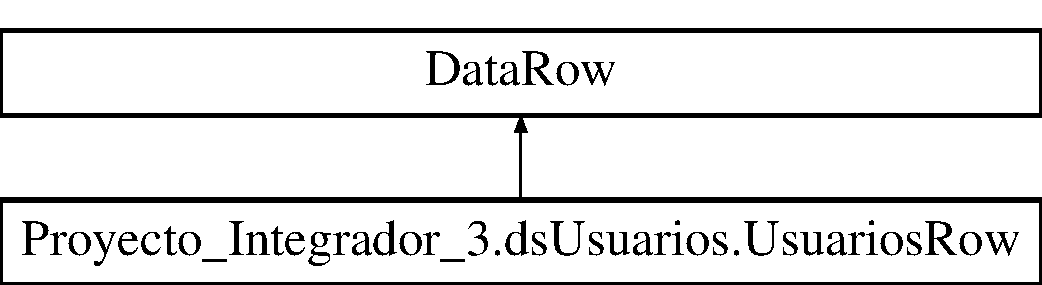
\includegraphics[height=2.000000cm]{d2/d7f/class_proyecto___integrador__3_1_1ds_usuarios_1_1_usuarios_row}
\end{center}
\end{figure}
\subsection*{Métodos públicos}
\begin{DoxyCompactItemize}
\item 
bool \hyperlink{class_proyecto___integrador__3_1_1ds_usuarios_1_1_usuarios_row_a8bd27421a1054b917ea8cf5d8ee022a5}{Is\-Nombre\-Null} ()
\item 
void \hyperlink{class_proyecto___integrador__3_1_1ds_usuarios_1_1_usuarios_row_a5056f9f0d604c17aeb58a4e8bc5a93d0}{Set\-Nombre\-Null} ()
\item 
bool \hyperlink{class_proyecto___integrador__3_1_1ds_usuarios_1_1_usuarios_row_a7a8d2746f278272b3d69a84ccb365c4f}{Is\-Calle\-Null} ()
\item 
void \hyperlink{class_proyecto___integrador__3_1_1ds_usuarios_1_1_usuarios_row_a517d7961e86d79b71e38907d8224334d}{Set\-Calle\-Null} ()
\item 
bool \hyperlink{class_proyecto___integrador__3_1_1ds_usuarios_1_1_usuarios_row_aac8b36d21a59fe1aaf5530dba9425968}{Is\-Telefono\-Null} ()
\item 
void \hyperlink{class_proyecto___integrador__3_1_1ds_usuarios_1_1_usuarios_row_a9a0244526cb1be6d40b9881de5c178d5}{Set\-Telefono\-Null} ()
\item 
bool \hyperlink{class_proyecto___integrador__3_1_1ds_usuarios_1_1_usuarios_row_ac0affeb4de860a91af002553e0c76bca}{Is\-Tipo\-Sangre\-Null} ()
\item 
void \hyperlink{class_proyecto___integrador__3_1_1ds_usuarios_1_1_usuarios_row_a7eeaf498704c6cbd4c632524319dd8bf}{Set\-Tipo\-Sangre\-Null} ()
\item 
bool \hyperlink{class_proyecto___integrador__3_1_1ds_usuarios_1_1_usuarios_row_a4d09dacf380262a3059cf42c59cf1d2a}{Is\-Alergias\-Null} ()
\item 
void \hyperlink{class_proyecto___integrador__3_1_1ds_usuarios_1_1_usuarios_row_a8e273c731e2573d37b46d606c65535e7}{Set\-Alergias\-Null} ()
\item 
bool \hyperlink{class_proyecto___integrador__3_1_1ds_usuarios_1_1_usuarios_row_a6deaacb2f4769f93f505f5dd9ac87648}{Is\-Nombre\-Contacto\-Null} ()
\item 
void \hyperlink{class_proyecto___integrador__3_1_1ds_usuarios_1_1_usuarios_row_a3b03343c0753d220ebc86951be8a7ae8}{Set\-Nombre\-Contacto\-Null} ()
\item 
bool \hyperlink{class_proyecto___integrador__3_1_1ds_usuarios_1_1_usuarios_row_aa217392e90d3440f1be9e2aa56335720}{Is\-Telefono\-Contacto\-Null} ()
\item 
void \hyperlink{class_proyecto___integrador__3_1_1ds_usuarios_1_1_usuarios_row_a6f1782a67618ee06a485d5b633ec464d}{Set\-Telefono\-Contacto\-Null} ()
\item 
bool \hyperlink{class_proyecto___integrador__3_1_1ds_usuarios_1_1_usuarios_row_a09309116f24e5c455b625cc6d06adb82}{Is\-Tipo\-Usuario\-Null} ()
\item 
void \hyperlink{class_proyecto___integrador__3_1_1ds_usuarios_1_1_usuarios_row_a71fd9bb2fc35514673578c3118e66ff3}{Set\-Tipo\-Usuario\-Null} ()
\item 
bool \hyperlink{class_proyecto___integrador__3_1_1ds_usuarios_1_1_usuarios_row_a92443a3dd51413248e7b27d7b3d9f758}{Is\-Saldo\-Null} ()
\item 
void \hyperlink{class_proyecto___integrador__3_1_1ds_usuarios_1_1_usuarios_row_a4d34e46fdae6f4181a12b9134b48a6ed}{Set\-Saldo\-Null} ()
\item 
bool \hyperlink{class_proyecto___integrador__3_1_1ds_usuarios_1_1_usuarios_row_ac962a7d6a957b31f1b25fc5e0b0c7c45}{Is\-Tarjeta\-Asignada\-Null} ()
\item 
void \hyperlink{class_proyecto___integrador__3_1_1ds_usuarios_1_1_usuarios_row_a69463821db8b47772bb0a85729eb39a7}{Set\-Tarjeta\-Asignada\-Null} ()
\item 
bool \hyperlink{class_proyecto___integrador__3_1_1ds_usuarios_1_1_usuarios_row_a24390db5126774844e377adf88c2469f}{Issexo\-Null} ()
\item 
void \hyperlink{class_proyecto___integrador__3_1_1ds_usuarios_1_1_usuarios_row_a4dbceacf3925b86203d5e506e31c774a}{Setsexo\-Null} ()
\item 
bool \hyperlink{class_proyecto___integrador__3_1_1ds_usuarios_1_1_usuarios_row_a30b17be77e21851cfdab66af76c984f9}{Is\-Fecha\-Nacimiento\-Null} ()
\item 
void \hyperlink{class_proyecto___integrador__3_1_1ds_usuarios_1_1_usuarios_row_ac1bafe8261b930f1594e50cc0ef4c1fc}{Set\-Fecha\-Nacimiento\-Null} ()
\item 
bool \hyperlink{class_proyecto___integrador__3_1_1ds_usuarios_1_1_usuarios_row_af7f8e7f33db7077fb17928de4b54d78b}{Is\-Numero\-Calle\-Null} ()
\item 
void \hyperlink{class_proyecto___integrador__3_1_1ds_usuarios_1_1_usuarios_row_a9bbca47e43232252616e83b04a99d52c}{Set\-Numero\-Calle\-Null} ()
\item 
bool \hyperlink{class_proyecto___integrador__3_1_1ds_usuarios_1_1_usuarios_row_ad756cb185f318c957103cc1470e098fa}{Is\-Colonia\-Null} ()
\item 
void \hyperlink{class_proyecto___integrador__3_1_1ds_usuarios_1_1_usuarios_row_ac466ee8841f0797f997cd4f058439fbf}{Set\-Colonia\-Null} ()
\item 
bool \hyperlink{class_proyecto___integrador__3_1_1ds_usuarios_1_1_usuarios_row_a16f077a1f2458872bb676a01c791e680}{Is\-Municipio\-Null} ()
\item 
void \hyperlink{class_proyecto___integrador__3_1_1ds_usuarios_1_1_usuarios_row_acd888a79fcad0d01ecbb9ed5bf545fa5}{Set\-Municipio\-Null} ()
\item 
bool \hyperlink{class_proyecto___integrador__3_1_1ds_usuarios_1_1_usuarios_row_a91df593253badb10ea5a851145664375}{Is\-Celular\-Null} ()
\item 
void \hyperlink{class_proyecto___integrador__3_1_1ds_usuarios_1_1_usuarios_row_a41d4aabf17b3c2d96a6fff800b2c5bb9}{Set\-Celular\-Null} ()
\end{DoxyCompactItemize}
\subsection*{Funciones del 'package'}
\begin{DoxyCompactItemize}
\item 
\hyperlink{class_proyecto___integrador__3_1_1ds_usuarios_1_1_usuarios_row_a6bff372090116bad1cbc7689a4309716}{Usuarios\-Row} (global\-::\-System.\-Data.\-Data\-Row\-Builder rb)
\end{DoxyCompactItemize}
\subsection*{Propiedades}
\begin{DoxyCompactItemize}
\item 
System.\-Guid \hyperlink{class_proyecto___integrador__3_1_1ds_usuarios_1_1_usuarios_row_a52527439e50952886c2ec1ddc5e06f3d}{Uid}\hspace{0.3cm}{\ttfamily  \mbox{[}get, set\mbox{]}}
\item 
string \hyperlink{class_proyecto___integrador__3_1_1ds_usuarios_1_1_usuarios_row_a7ae7f1dd4b1d6edfab95ee9789ad44e0}{Nombre}\hspace{0.3cm}{\ttfamily  \mbox{[}get, set\mbox{]}}
\item 
string \hyperlink{class_proyecto___integrador__3_1_1ds_usuarios_1_1_usuarios_row_a0886bce094a8baf1cdcb8fccf0345c48}{Calle}\hspace{0.3cm}{\ttfamily  \mbox{[}get, set\mbox{]}}
\item 
string \hyperlink{class_proyecto___integrador__3_1_1ds_usuarios_1_1_usuarios_row_aed26f4593a25f2cbea2d3fb95c032d75}{Telefono}\hspace{0.3cm}{\ttfamily  \mbox{[}get, set\mbox{]}}
\item 
int \hyperlink{class_proyecto___integrador__3_1_1ds_usuarios_1_1_usuarios_row_a1ca1a500a2d31c6c84e6faa942815804}{Tipo\-Sangre}\hspace{0.3cm}{\ttfamily  \mbox{[}get, set\mbox{]}}
\item 
string \hyperlink{class_proyecto___integrador__3_1_1ds_usuarios_1_1_usuarios_row_ac7fdabb96c11d7f4fec61e676d01f897}{Alergias}\hspace{0.3cm}{\ttfamily  \mbox{[}get, set\mbox{]}}
\item 
string \hyperlink{class_proyecto___integrador__3_1_1ds_usuarios_1_1_usuarios_row_aec944b13be287218767cf4fe5abefbe5}{Nombre\-Contacto}\hspace{0.3cm}{\ttfamily  \mbox{[}get, set\mbox{]}}
\item 
string \hyperlink{class_proyecto___integrador__3_1_1ds_usuarios_1_1_usuarios_row_a0a97576bc8d3b21e8e6c4f2554759fa0}{Telefono\-Contacto}\hspace{0.3cm}{\ttfamily  \mbox{[}get, set\mbox{]}}
\item 
byte \hyperlink{class_proyecto___integrador__3_1_1ds_usuarios_1_1_usuarios_row_ab4f44ba81813ff94a806d2cf0ff99415}{Tipo\-Usuario}\hspace{0.3cm}{\ttfamily  \mbox{[}get, set\mbox{]}}
\item 
decimal \hyperlink{class_proyecto___integrador__3_1_1ds_usuarios_1_1_usuarios_row_a8767d20d2bfa9f4e265f9bb2fb38fffd}{Saldo}\hspace{0.3cm}{\ttfamily  \mbox{[}get, set\mbox{]}}
\item 
string \hyperlink{class_proyecto___integrador__3_1_1ds_usuarios_1_1_usuarios_row_aa22b95dee1aa553d36348fd272f7bf51}{Tarjeta\-Asignada}\hspace{0.3cm}{\ttfamily  \mbox{[}get, set\mbox{]}}
\item 
bool \hyperlink{class_proyecto___integrador__3_1_1ds_usuarios_1_1_usuarios_row_a459ef01bf05692c7b43e376b3d6620b5}{sexo}\hspace{0.3cm}{\ttfamily  \mbox{[}get, set\mbox{]}}
\item 
System.\-Date\-Time \hyperlink{class_proyecto___integrador__3_1_1ds_usuarios_1_1_usuarios_row_afa3832e8eeb4e9b652518de75e15b432}{Fecha\-Nacimiento}\hspace{0.3cm}{\ttfamily  \mbox{[}get, set\mbox{]}}
\item 
int \hyperlink{class_proyecto___integrador__3_1_1ds_usuarios_1_1_usuarios_row_aa0af07f9536d8af14cabf3e7c7db4055}{Numero\-Calle}\hspace{0.3cm}{\ttfamily  \mbox{[}get, set\mbox{]}}
\item 
string \hyperlink{class_proyecto___integrador__3_1_1ds_usuarios_1_1_usuarios_row_a799b567271f5d75af1532e54ce6df2d7}{Colonia}\hspace{0.3cm}{\ttfamily  \mbox{[}get, set\mbox{]}}
\item 
short \hyperlink{class_proyecto___integrador__3_1_1ds_usuarios_1_1_usuarios_row_a041ccccf07ecbeb1feb041650c93be2a}{Municipio}\hspace{0.3cm}{\ttfamily  \mbox{[}get, set\mbox{]}}
\item 
string \hyperlink{class_proyecto___integrador__3_1_1ds_usuarios_1_1_usuarios_row_abed4782f1967d4f2fefeb7f8c23d4edb}{Celular}\hspace{0.3cm}{\ttfamily  \mbox{[}get, set\mbox{]}}
\end{DoxyCompactItemize}
\subsection*{Atributos privados}
\begin{DoxyCompactItemize}
\item 
\hyperlink{class_proyecto___integrador__3_1_1ds_usuarios_1_1_usuarios_data_table}{Usuarios\-Data\-Table} \hyperlink{class_proyecto___integrador__3_1_1ds_usuarios_1_1_usuarios_row_aafda5a6bdd7b0b2149e77517e78f56d2}{table\-Usuarios}
\end{DoxyCompactItemize}


\subsection{Descripción detallada}
Represents strongly named Data\-Row class. 

/summary$>$ 

Definición en la línea 786 del archivo ds\-Usuarios.\-Designer.\-cs.



\subsection{Documentación del constructor y destructor}
\hypertarget{class_proyecto___integrador__3_1_1ds_usuarios_1_1_usuarios_row_a6bff372090116bad1cbc7689a4309716}{\index{Proyecto\-\_\-\-Integrador\-\_\-3\-::ds\-Usuarios\-::\-Usuarios\-Row@{Proyecto\-\_\-\-Integrador\-\_\-3\-::ds\-Usuarios\-::\-Usuarios\-Row}!Usuarios\-Row@{Usuarios\-Row}}
\index{Usuarios\-Row@{Usuarios\-Row}!Proyecto_Integrador_3::dsUsuarios::UsuariosRow@{Proyecto\-\_\-\-Integrador\-\_\-3\-::ds\-Usuarios\-::\-Usuarios\-Row}}
\subsubsection[{Usuarios\-Row}]{\setlength{\rightskip}{0pt plus 5cm}Proyecto\-\_\-\-Integrador\-\_\-3.\-ds\-Usuarios.\-Usuarios\-Row.\-Usuarios\-Row (
\begin{DoxyParamCaption}
\item[{global\-::\-System.\-Data.\-Data\-Row\-Builder}]{rb}
\end{DoxyParamCaption}
)\hspace{0.3cm}{\ttfamily [inline]}, {\ttfamily [package]}}}\label{class_proyecto___integrador__3_1_1ds_usuarios_1_1_usuarios_row_a6bff372090116bad1cbc7689a4309716}


Definición en la línea 792 del archivo ds\-Usuarios.\-Designer.\-cs.


\begin{DoxyCode}
792                                                                       : 
793                     base(rb) \{
794                 this.\hyperlink{class_proyecto___integrador__3_1_1ds_usuarios_1_1_usuarios_row_aafda5a6bdd7b0b2149e77517e78f56d2}{tableUsuarios} = ((UsuariosDataTable)(this.Table));
795             \}
\end{DoxyCode}


\subsection{Documentación de las funciones miembro}
\hypertarget{class_proyecto___integrador__3_1_1ds_usuarios_1_1_usuarios_row_a4d09dacf380262a3059cf42c59cf1d2a}{\index{Proyecto\-\_\-\-Integrador\-\_\-3\-::ds\-Usuarios\-::\-Usuarios\-Row@{Proyecto\-\_\-\-Integrador\-\_\-3\-::ds\-Usuarios\-::\-Usuarios\-Row}!Is\-Alergias\-Null@{Is\-Alergias\-Null}}
\index{Is\-Alergias\-Null@{Is\-Alergias\-Null}!Proyecto_Integrador_3::dsUsuarios::UsuariosRow@{Proyecto\-\_\-\-Integrador\-\_\-3\-::ds\-Usuarios\-::\-Usuarios\-Row}}
\subsubsection[{Is\-Alergias\-Null}]{\setlength{\rightskip}{0pt plus 5cm}bool Proyecto\-\_\-\-Integrador\-\_\-3.\-ds\-Usuarios.\-Usuarios\-Row.\-Is\-Alergias\-Null (
\begin{DoxyParamCaption}
{}
\end{DoxyParamCaption}
)\hspace{0.3cm}{\ttfamily [inline]}}}\label{class_proyecto___integrador__3_1_1ds_usuarios_1_1_usuarios_row_a4d09dacf380262a3059cf42c59cf1d2a}


Definición en la línea 1114 del archivo ds\-Usuarios.\-Designer.\-cs.


\begin{DoxyCode}
1114                                          \{
1115                 \textcolor{keywordflow}{return} this.IsNull(this.\hyperlink{class_proyecto___integrador__3_1_1ds_usuarios_1_1_usuarios_row_aafda5a6bdd7b0b2149e77517e78f56d2}{tableUsuarios}.
      \hyperlink{class_proyecto___integrador__3_1_1ds_usuarios_1_1_usuarios_data_table_ae6535f8c6396d4fc1073655a15c1207d}{AlergiasColumn});
1116             \}
\end{DoxyCode}
\hypertarget{class_proyecto___integrador__3_1_1ds_usuarios_1_1_usuarios_row_a7a8d2746f278272b3d69a84ccb365c4f}{\index{Proyecto\-\_\-\-Integrador\-\_\-3\-::ds\-Usuarios\-::\-Usuarios\-Row@{Proyecto\-\_\-\-Integrador\-\_\-3\-::ds\-Usuarios\-::\-Usuarios\-Row}!Is\-Calle\-Null@{Is\-Calle\-Null}}
\index{Is\-Calle\-Null@{Is\-Calle\-Null}!Proyecto_Integrador_3::dsUsuarios::UsuariosRow@{Proyecto\-\_\-\-Integrador\-\_\-3\-::ds\-Usuarios\-::\-Usuarios\-Row}}
\subsubsection[{Is\-Calle\-Null}]{\setlength{\rightskip}{0pt plus 5cm}bool Proyecto\-\_\-\-Integrador\-\_\-3.\-ds\-Usuarios.\-Usuarios\-Row.\-Is\-Calle\-Null (
\begin{DoxyParamCaption}
{}
\end{DoxyParamCaption}
)\hspace{0.3cm}{\ttfamily [inline]}}}\label{class_proyecto___integrador__3_1_1ds_usuarios_1_1_usuarios_row_a7a8d2746f278272b3d69a84ccb365c4f}


Definición en la línea 1078 del archivo ds\-Usuarios.\-Designer.\-cs.


\begin{DoxyCode}
1078                                       \{
1079                 \textcolor{keywordflow}{return} this.IsNull(this.\hyperlink{class_proyecto___integrador__3_1_1ds_usuarios_1_1_usuarios_row_aafda5a6bdd7b0b2149e77517e78f56d2}{tableUsuarios}.\hyperlink{class_proyecto___integrador__3_1_1ds_usuarios_1_1_usuarios_data_table_acbf55d075ab35bd85f1efb354bb744b4}{CalleColumn});
1080             \}
\end{DoxyCode}
\hypertarget{class_proyecto___integrador__3_1_1ds_usuarios_1_1_usuarios_row_a91df593253badb10ea5a851145664375}{\index{Proyecto\-\_\-\-Integrador\-\_\-3\-::ds\-Usuarios\-::\-Usuarios\-Row@{Proyecto\-\_\-\-Integrador\-\_\-3\-::ds\-Usuarios\-::\-Usuarios\-Row}!Is\-Celular\-Null@{Is\-Celular\-Null}}
\index{Is\-Celular\-Null@{Is\-Celular\-Null}!Proyecto_Integrador_3::dsUsuarios::UsuariosRow@{Proyecto\-\_\-\-Integrador\-\_\-3\-::ds\-Usuarios\-::\-Usuarios\-Row}}
\subsubsection[{Is\-Celular\-Null}]{\setlength{\rightskip}{0pt plus 5cm}bool Proyecto\-\_\-\-Integrador\-\_\-3.\-ds\-Usuarios.\-Usuarios\-Row.\-Is\-Celular\-Null (
\begin{DoxyParamCaption}
{}
\end{DoxyParamCaption}
)\hspace{0.3cm}{\ttfamily [inline]}}}\label{class_proyecto___integrador__3_1_1ds_usuarios_1_1_usuarios_row_a91df593253badb10ea5a851145664375}


Definición en la línea 1246 del archivo ds\-Usuarios.\-Designer.\-cs.


\begin{DoxyCode}
1246                                         \{
1247                 \textcolor{keywordflow}{return} this.IsNull(this.\hyperlink{class_proyecto___integrador__3_1_1ds_usuarios_1_1_usuarios_row_aafda5a6bdd7b0b2149e77517e78f56d2}{tableUsuarios}.\hyperlink{class_proyecto___integrador__3_1_1ds_usuarios_1_1_usuarios_data_table_ab00350fd3b8bd2f7f26fdd22da40cf47}{CelularColumn});
1248             \}
\end{DoxyCode}
\hypertarget{class_proyecto___integrador__3_1_1ds_usuarios_1_1_usuarios_row_ad756cb185f318c957103cc1470e098fa}{\index{Proyecto\-\_\-\-Integrador\-\_\-3\-::ds\-Usuarios\-::\-Usuarios\-Row@{Proyecto\-\_\-\-Integrador\-\_\-3\-::ds\-Usuarios\-::\-Usuarios\-Row}!Is\-Colonia\-Null@{Is\-Colonia\-Null}}
\index{Is\-Colonia\-Null@{Is\-Colonia\-Null}!Proyecto_Integrador_3::dsUsuarios::UsuariosRow@{Proyecto\-\_\-\-Integrador\-\_\-3\-::ds\-Usuarios\-::\-Usuarios\-Row}}
\subsubsection[{Is\-Colonia\-Null}]{\setlength{\rightskip}{0pt plus 5cm}bool Proyecto\-\_\-\-Integrador\-\_\-3.\-ds\-Usuarios.\-Usuarios\-Row.\-Is\-Colonia\-Null (
\begin{DoxyParamCaption}
{}
\end{DoxyParamCaption}
)\hspace{0.3cm}{\ttfamily [inline]}}}\label{class_proyecto___integrador__3_1_1ds_usuarios_1_1_usuarios_row_ad756cb185f318c957103cc1470e098fa}


Definición en la línea 1222 del archivo ds\-Usuarios.\-Designer.\-cs.


\begin{DoxyCode}
1222                                         \{
1223                 \textcolor{keywordflow}{return} this.IsNull(this.\hyperlink{class_proyecto___integrador__3_1_1ds_usuarios_1_1_usuarios_row_aafda5a6bdd7b0b2149e77517e78f56d2}{tableUsuarios}.\hyperlink{class_proyecto___integrador__3_1_1ds_usuarios_1_1_usuarios_data_table_a9279b22c7066920de7247faff42868b2}{ColoniaColumn});
1224             \}
\end{DoxyCode}
\hypertarget{class_proyecto___integrador__3_1_1ds_usuarios_1_1_usuarios_row_a30b17be77e21851cfdab66af76c984f9}{\index{Proyecto\-\_\-\-Integrador\-\_\-3\-::ds\-Usuarios\-::\-Usuarios\-Row@{Proyecto\-\_\-\-Integrador\-\_\-3\-::ds\-Usuarios\-::\-Usuarios\-Row}!Is\-Fecha\-Nacimiento\-Null@{Is\-Fecha\-Nacimiento\-Null}}
\index{Is\-Fecha\-Nacimiento\-Null@{Is\-Fecha\-Nacimiento\-Null}!Proyecto_Integrador_3::dsUsuarios::UsuariosRow@{Proyecto\-\_\-\-Integrador\-\_\-3\-::ds\-Usuarios\-::\-Usuarios\-Row}}
\subsubsection[{Is\-Fecha\-Nacimiento\-Null}]{\setlength{\rightskip}{0pt plus 5cm}bool Proyecto\-\_\-\-Integrador\-\_\-3.\-ds\-Usuarios.\-Usuarios\-Row.\-Is\-Fecha\-Nacimiento\-Null (
\begin{DoxyParamCaption}
{}
\end{DoxyParamCaption}
)\hspace{0.3cm}{\ttfamily [inline]}}}\label{class_proyecto___integrador__3_1_1ds_usuarios_1_1_usuarios_row_a30b17be77e21851cfdab66af76c984f9}


Definición en la línea 1198 del archivo ds\-Usuarios.\-Designer.\-cs.


\begin{DoxyCode}
1198                                                 \{
1199                 \textcolor{keywordflow}{return} this.IsNull(this.\hyperlink{class_proyecto___integrador__3_1_1ds_usuarios_1_1_usuarios_row_aafda5a6bdd7b0b2149e77517e78f56d2}{tableUsuarios}.
      \hyperlink{class_proyecto___integrador__3_1_1ds_usuarios_1_1_usuarios_data_table_a4c55af9308924a62ce21d93b85837246}{FechaNacimientoColumn});
1200             \}
\end{DoxyCode}
\hypertarget{class_proyecto___integrador__3_1_1ds_usuarios_1_1_usuarios_row_a16f077a1f2458872bb676a01c791e680}{\index{Proyecto\-\_\-\-Integrador\-\_\-3\-::ds\-Usuarios\-::\-Usuarios\-Row@{Proyecto\-\_\-\-Integrador\-\_\-3\-::ds\-Usuarios\-::\-Usuarios\-Row}!Is\-Municipio\-Null@{Is\-Municipio\-Null}}
\index{Is\-Municipio\-Null@{Is\-Municipio\-Null}!Proyecto_Integrador_3::dsUsuarios::UsuariosRow@{Proyecto\-\_\-\-Integrador\-\_\-3\-::ds\-Usuarios\-::\-Usuarios\-Row}}
\subsubsection[{Is\-Municipio\-Null}]{\setlength{\rightskip}{0pt plus 5cm}bool Proyecto\-\_\-\-Integrador\-\_\-3.\-ds\-Usuarios.\-Usuarios\-Row.\-Is\-Municipio\-Null (
\begin{DoxyParamCaption}
{}
\end{DoxyParamCaption}
)\hspace{0.3cm}{\ttfamily [inline]}}}\label{class_proyecto___integrador__3_1_1ds_usuarios_1_1_usuarios_row_a16f077a1f2458872bb676a01c791e680}


Definición en la línea 1234 del archivo ds\-Usuarios.\-Designer.\-cs.


\begin{DoxyCode}
1234                                           \{
1235                 \textcolor{keywordflow}{return} this.IsNull(this.\hyperlink{class_proyecto___integrador__3_1_1ds_usuarios_1_1_usuarios_row_aafda5a6bdd7b0b2149e77517e78f56d2}{tableUsuarios}.
      \hyperlink{class_proyecto___integrador__3_1_1ds_usuarios_1_1_usuarios_data_table_aa62b66be9729351bbc91dcf69f60f0a0}{MunicipioColumn});
1236             \}
\end{DoxyCode}
\hypertarget{class_proyecto___integrador__3_1_1ds_usuarios_1_1_usuarios_row_a6deaacb2f4769f93f505f5dd9ac87648}{\index{Proyecto\-\_\-\-Integrador\-\_\-3\-::ds\-Usuarios\-::\-Usuarios\-Row@{Proyecto\-\_\-\-Integrador\-\_\-3\-::ds\-Usuarios\-::\-Usuarios\-Row}!Is\-Nombre\-Contacto\-Null@{Is\-Nombre\-Contacto\-Null}}
\index{Is\-Nombre\-Contacto\-Null@{Is\-Nombre\-Contacto\-Null}!Proyecto_Integrador_3::dsUsuarios::UsuariosRow@{Proyecto\-\_\-\-Integrador\-\_\-3\-::ds\-Usuarios\-::\-Usuarios\-Row}}
\subsubsection[{Is\-Nombre\-Contacto\-Null}]{\setlength{\rightskip}{0pt plus 5cm}bool Proyecto\-\_\-\-Integrador\-\_\-3.\-ds\-Usuarios.\-Usuarios\-Row.\-Is\-Nombre\-Contacto\-Null (
\begin{DoxyParamCaption}
{}
\end{DoxyParamCaption}
)\hspace{0.3cm}{\ttfamily [inline]}}}\label{class_proyecto___integrador__3_1_1ds_usuarios_1_1_usuarios_row_a6deaacb2f4769f93f505f5dd9ac87648}


Definición en la línea 1126 del archivo ds\-Usuarios.\-Designer.\-cs.


\begin{DoxyCode}
1126                                                \{
1127                 \textcolor{keywordflow}{return} this.IsNull(this.\hyperlink{class_proyecto___integrador__3_1_1ds_usuarios_1_1_usuarios_row_aafda5a6bdd7b0b2149e77517e78f56d2}{tableUsuarios}.
      \hyperlink{class_proyecto___integrador__3_1_1ds_usuarios_1_1_usuarios_data_table_ad0071571b88896ada8f0747ec5e441e2}{NombreContactoColumn});
1128             \}
\end{DoxyCode}
\hypertarget{class_proyecto___integrador__3_1_1ds_usuarios_1_1_usuarios_row_a8bd27421a1054b917ea8cf5d8ee022a5}{\index{Proyecto\-\_\-\-Integrador\-\_\-3\-::ds\-Usuarios\-::\-Usuarios\-Row@{Proyecto\-\_\-\-Integrador\-\_\-3\-::ds\-Usuarios\-::\-Usuarios\-Row}!Is\-Nombre\-Null@{Is\-Nombre\-Null}}
\index{Is\-Nombre\-Null@{Is\-Nombre\-Null}!Proyecto_Integrador_3::dsUsuarios::UsuariosRow@{Proyecto\-\_\-\-Integrador\-\_\-3\-::ds\-Usuarios\-::\-Usuarios\-Row}}
\subsubsection[{Is\-Nombre\-Null}]{\setlength{\rightskip}{0pt plus 5cm}bool Proyecto\-\_\-\-Integrador\-\_\-3.\-ds\-Usuarios.\-Usuarios\-Row.\-Is\-Nombre\-Null (
\begin{DoxyParamCaption}
{}
\end{DoxyParamCaption}
)\hspace{0.3cm}{\ttfamily [inline]}}}\label{class_proyecto___integrador__3_1_1ds_usuarios_1_1_usuarios_row_a8bd27421a1054b917ea8cf5d8ee022a5}


Definición en la línea 1066 del archivo ds\-Usuarios.\-Designer.\-cs.


\begin{DoxyCode}
1066                                        \{
1067                 \textcolor{keywordflow}{return} this.IsNull(this.\hyperlink{class_proyecto___integrador__3_1_1ds_usuarios_1_1_usuarios_row_aafda5a6bdd7b0b2149e77517e78f56d2}{tableUsuarios}.\hyperlink{class_proyecto___integrador__3_1_1ds_usuarios_1_1_usuarios_data_table_aa73ca2ed9aaabb05af840aac3bd943f5}{NombreColumn});
1068             \}
\end{DoxyCode}
\hypertarget{class_proyecto___integrador__3_1_1ds_usuarios_1_1_usuarios_row_af7f8e7f33db7077fb17928de4b54d78b}{\index{Proyecto\-\_\-\-Integrador\-\_\-3\-::ds\-Usuarios\-::\-Usuarios\-Row@{Proyecto\-\_\-\-Integrador\-\_\-3\-::ds\-Usuarios\-::\-Usuarios\-Row}!Is\-Numero\-Calle\-Null@{Is\-Numero\-Calle\-Null}}
\index{Is\-Numero\-Calle\-Null@{Is\-Numero\-Calle\-Null}!Proyecto_Integrador_3::dsUsuarios::UsuariosRow@{Proyecto\-\_\-\-Integrador\-\_\-3\-::ds\-Usuarios\-::\-Usuarios\-Row}}
\subsubsection[{Is\-Numero\-Calle\-Null}]{\setlength{\rightskip}{0pt plus 5cm}bool Proyecto\-\_\-\-Integrador\-\_\-3.\-ds\-Usuarios.\-Usuarios\-Row.\-Is\-Numero\-Calle\-Null (
\begin{DoxyParamCaption}
{}
\end{DoxyParamCaption}
)\hspace{0.3cm}{\ttfamily [inline]}}}\label{class_proyecto___integrador__3_1_1ds_usuarios_1_1_usuarios_row_af7f8e7f33db7077fb17928de4b54d78b}


Definición en la línea 1210 del archivo ds\-Usuarios.\-Designer.\-cs.


\begin{DoxyCode}
1210                                             \{
1211                 \textcolor{keywordflow}{return} this.IsNull(this.\hyperlink{class_proyecto___integrador__3_1_1ds_usuarios_1_1_usuarios_row_aafda5a6bdd7b0b2149e77517e78f56d2}{tableUsuarios}.
      \hyperlink{class_proyecto___integrador__3_1_1ds_usuarios_1_1_usuarios_data_table_a442769603ef31cf87b2a9fef73b9851e}{NumeroCalleColumn});
1212             \}
\end{DoxyCode}
\hypertarget{class_proyecto___integrador__3_1_1ds_usuarios_1_1_usuarios_row_a92443a3dd51413248e7b27d7b3d9f758}{\index{Proyecto\-\_\-\-Integrador\-\_\-3\-::ds\-Usuarios\-::\-Usuarios\-Row@{Proyecto\-\_\-\-Integrador\-\_\-3\-::ds\-Usuarios\-::\-Usuarios\-Row}!Is\-Saldo\-Null@{Is\-Saldo\-Null}}
\index{Is\-Saldo\-Null@{Is\-Saldo\-Null}!Proyecto_Integrador_3::dsUsuarios::UsuariosRow@{Proyecto\-\_\-\-Integrador\-\_\-3\-::ds\-Usuarios\-::\-Usuarios\-Row}}
\subsubsection[{Is\-Saldo\-Null}]{\setlength{\rightskip}{0pt plus 5cm}bool Proyecto\-\_\-\-Integrador\-\_\-3.\-ds\-Usuarios.\-Usuarios\-Row.\-Is\-Saldo\-Null (
\begin{DoxyParamCaption}
{}
\end{DoxyParamCaption}
)\hspace{0.3cm}{\ttfamily [inline]}}}\label{class_proyecto___integrador__3_1_1ds_usuarios_1_1_usuarios_row_a92443a3dd51413248e7b27d7b3d9f758}


Definición en la línea 1162 del archivo ds\-Usuarios.\-Designer.\-cs.


\begin{DoxyCode}
1162                                       \{
1163                 \textcolor{keywordflow}{return} this.IsNull(this.\hyperlink{class_proyecto___integrador__3_1_1ds_usuarios_1_1_usuarios_row_aafda5a6bdd7b0b2149e77517e78f56d2}{tableUsuarios}.\hyperlink{class_proyecto___integrador__3_1_1ds_usuarios_1_1_usuarios_data_table_a0e728022751a9d5dffae82c0e1b66ade}{SaldoColumn});
1164             \}
\end{DoxyCode}
\hypertarget{class_proyecto___integrador__3_1_1ds_usuarios_1_1_usuarios_row_a24390db5126774844e377adf88c2469f}{\index{Proyecto\-\_\-\-Integrador\-\_\-3\-::ds\-Usuarios\-::\-Usuarios\-Row@{Proyecto\-\_\-\-Integrador\-\_\-3\-::ds\-Usuarios\-::\-Usuarios\-Row}!Issexo\-Null@{Issexo\-Null}}
\index{Issexo\-Null@{Issexo\-Null}!Proyecto_Integrador_3::dsUsuarios::UsuariosRow@{Proyecto\-\_\-\-Integrador\-\_\-3\-::ds\-Usuarios\-::\-Usuarios\-Row}}
\subsubsection[{Issexo\-Null}]{\setlength{\rightskip}{0pt plus 5cm}bool Proyecto\-\_\-\-Integrador\-\_\-3.\-ds\-Usuarios.\-Usuarios\-Row.\-Issexo\-Null (
\begin{DoxyParamCaption}
{}
\end{DoxyParamCaption}
)\hspace{0.3cm}{\ttfamily [inline]}}}\label{class_proyecto___integrador__3_1_1ds_usuarios_1_1_usuarios_row_a24390db5126774844e377adf88c2469f}


Definición en la línea 1186 del archivo ds\-Usuarios.\-Designer.\-cs.


\begin{DoxyCode}
1186                                      \{
1187                 \textcolor{keywordflow}{return} this.IsNull(this.\hyperlink{class_proyecto___integrador__3_1_1ds_usuarios_1_1_usuarios_row_aafda5a6bdd7b0b2149e77517e78f56d2}{tableUsuarios}.\hyperlink{class_proyecto___integrador__3_1_1ds_usuarios_1_1_usuarios_data_table_a900ede3b64e19670a69d7ad762ab1695}{sexoColumn});
1188             \}
\end{DoxyCode}
\hypertarget{class_proyecto___integrador__3_1_1ds_usuarios_1_1_usuarios_row_ac962a7d6a957b31f1b25fc5e0b0c7c45}{\index{Proyecto\-\_\-\-Integrador\-\_\-3\-::ds\-Usuarios\-::\-Usuarios\-Row@{Proyecto\-\_\-\-Integrador\-\_\-3\-::ds\-Usuarios\-::\-Usuarios\-Row}!Is\-Tarjeta\-Asignada\-Null@{Is\-Tarjeta\-Asignada\-Null}}
\index{Is\-Tarjeta\-Asignada\-Null@{Is\-Tarjeta\-Asignada\-Null}!Proyecto_Integrador_3::dsUsuarios::UsuariosRow@{Proyecto\-\_\-\-Integrador\-\_\-3\-::ds\-Usuarios\-::\-Usuarios\-Row}}
\subsubsection[{Is\-Tarjeta\-Asignada\-Null}]{\setlength{\rightskip}{0pt plus 5cm}bool Proyecto\-\_\-\-Integrador\-\_\-3.\-ds\-Usuarios.\-Usuarios\-Row.\-Is\-Tarjeta\-Asignada\-Null (
\begin{DoxyParamCaption}
{}
\end{DoxyParamCaption}
)\hspace{0.3cm}{\ttfamily [inline]}}}\label{class_proyecto___integrador__3_1_1ds_usuarios_1_1_usuarios_row_ac962a7d6a957b31f1b25fc5e0b0c7c45}


Definición en la línea 1174 del archivo ds\-Usuarios.\-Designer.\-cs.


\begin{DoxyCode}
1174                                                 \{
1175                 \textcolor{keywordflow}{return} this.IsNull(this.\hyperlink{class_proyecto___integrador__3_1_1ds_usuarios_1_1_usuarios_row_aafda5a6bdd7b0b2149e77517e78f56d2}{tableUsuarios}.
      \hyperlink{class_proyecto___integrador__3_1_1ds_usuarios_1_1_usuarios_data_table_adaf2cdbd83042f6ed4c524deec1469d4}{TarjetaAsignadaColumn});
1176             \}
\end{DoxyCode}
\hypertarget{class_proyecto___integrador__3_1_1ds_usuarios_1_1_usuarios_row_aa217392e90d3440f1be9e2aa56335720}{\index{Proyecto\-\_\-\-Integrador\-\_\-3\-::ds\-Usuarios\-::\-Usuarios\-Row@{Proyecto\-\_\-\-Integrador\-\_\-3\-::ds\-Usuarios\-::\-Usuarios\-Row}!Is\-Telefono\-Contacto\-Null@{Is\-Telefono\-Contacto\-Null}}
\index{Is\-Telefono\-Contacto\-Null@{Is\-Telefono\-Contacto\-Null}!Proyecto_Integrador_3::dsUsuarios::UsuariosRow@{Proyecto\-\_\-\-Integrador\-\_\-3\-::ds\-Usuarios\-::\-Usuarios\-Row}}
\subsubsection[{Is\-Telefono\-Contacto\-Null}]{\setlength{\rightskip}{0pt plus 5cm}bool Proyecto\-\_\-\-Integrador\-\_\-3.\-ds\-Usuarios.\-Usuarios\-Row.\-Is\-Telefono\-Contacto\-Null (
\begin{DoxyParamCaption}
{}
\end{DoxyParamCaption}
)\hspace{0.3cm}{\ttfamily [inline]}}}\label{class_proyecto___integrador__3_1_1ds_usuarios_1_1_usuarios_row_aa217392e90d3440f1be9e2aa56335720}


Definición en la línea 1138 del archivo ds\-Usuarios.\-Designer.\-cs.


\begin{DoxyCode}
1138                                                  \{
1139                 \textcolor{keywordflow}{return} this.IsNull(this.\hyperlink{class_proyecto___integrador__3_1_1ds_usuarios_1_1_usuarios_row_aafda5a6bdd7b0b2149e77517e78f56d2}{tableUsuarios}.
      \hyperlink{class_proyecto___integrador__3_1_1ds_usuarios_1_1_usuarios_data_table_aab76d3089d1ea9ee22016e085deace10}{TelefonoContactoColumn});
1140             \}
\end{DoxyCode}
\hypertarget{class_proyecto___integrador__3_1_1ds_usuarios_1_1_usuarios_row_aac8b36d21a59fe1aaf5530dba9425968}{\index{Proyecto\-\_\-\-Integrador\-\_\-3\-::ds\-Usuarios\-::\-Usuarios\-Row@{Proyecto\-\_\-\-Integrador\-\_\-3\-::ds\-Usuarios\-::\-Usuarios\-Row}!Is\-Telefono\-Null@{Is\-Telefono\-Null}}
\index{Is\-Telefono\-Null@{Is\-Telefono\-Null}!Proyecto_Integrador_3::dsUsuarios::UsuariosRow@{Proyecto\-\_\-\-Integrador\-\_\-3\-::ds\-Usuarios\-::\-Usuarios\-Row}}
\subsubsection[{Is\-Telefono\-Null}]{\setlength{\rightskip}{0pt plus 5cm}bool Proyecto\-\_\-\-Integrador\-\_\-3.\-ds\-Usuarios.\-Usuarios\-Row.\-Is\-Telefono\-Null (
\begin{DoxyParamCaption}
{}
\end{DoxyParamCaption}
)\hspace{0.3cm}{\ttfamily [inline]}}}\label{class_proyecto___integrador__3_1_1ds_usuarios_1_1_usuarios_row_aac8b36d21a59fe1aaf5530dba9425968}


Definición en la línea 1090 del archivo ds\-Usuarios.\-Designer.\-cs.


\begin{DoxyCode}
1090                                          \{
1091                 \textcolor{keywordflow}{return} this.IsNull(this.\hyperlink{class_proyecto___integrador__3_1_1ds_usuarios_1_1_usuarios_row_aafda5a6bdd7b0b2149e77517e78f56d2}{tableUsuarios}.
      \hyperlink{class_proyecto___integrador__3_1_1ds_usuarios_1_1_usuarios_data_table_ac740a752802c6cb9a3ed8f4c1990f750}{TelefonoColumn});
1092             \}
\end{DoxyCode}
\hypertarget{class_proyecto___integrador__3_1_1ds_usuarios_1_1_usuarios_row_ac0affeb4de860a91af002553e0c76bca}{\index{Proyecto\-\_\-\-Integrador\-\_\-3\-::ds\-Usuarios\-::\-Usuarios\-Row@{Proyecto\-\_\-\-Integrador\-\_\-3\-::ds\-Usuarios\-::\-Usuarios\-Row}!Is\-Tipo\-Sangre\-Null@{Is\-Tipo\-Sangre\-Null}}
\index{Is\-Tipo\-Sangre\-Null@{Is\-Tipo\-Sangre\-Null}!Proyecto_Integrador_3::dsUsuarios::UsuariosRow@{Proyecto\-\_\-\-Integrador\-\_\-3\-::ds\-Usuarios\-::\-Usuarios\-Row}}
\subsubsection[{Is\-Tipo\-Sangre\-Null}]{\setlength{\rightskip}{0pt plus 5cm}bool Proyecto\-\_\-\-Integrador\-\_\-3.\-ds\-Usuarios.\-Usuarios\-Row.\-Is\-Tipo\-Sangre\-Null (
\begin{DoxyParamCaption}
{}
\end{DoxyParamCaption}
)\hspace{0.3cm}{\ttfamily [inline]}}}\label{class_proyecto___integrador__3_1_1ds_usuarios_1_1_usuarios_row_ac0affeb4de860a91af002553e0c76bca}


Definición en la línea 1102 del archivo ds\-Usuarios.\-Designer.\-cs.


\begin{DoxyCode}
1102                                            \{
1103                 \textcolor{keywordflow}{return} this.IsNull(this.\hyperlink{class_proyecto___integrador__3_1_1ds_usuarios_1_1_usuarios_row_aafda5a6bdd7b0b2149e77517e78f56d2}{tableUsuarios}.
      \hyperlink{class_proyecto___integrador__3_1_1ds_usuarios_1_1_usuarios_data_table_a73c18d0ad197d7314db69321b8d77d96}{TipoSangreColumn});
1104             \}
\end{DoxyCode}
\hypertarget{class_proyecto___integrador__3_1_1ds_usuarios_1_1_usuarios_row_a09309116f24e5c455b625cc6d06adb82}{\index{Proyecto\-\_\-\-Integrador\-\_\-3\-::ds\-Usuarios\-::\-Usuarios\-Row@{Proyecto\-\_\-\-Integrador\-\_\-3\-::ds\-Usuarios\-::\-Usuarios\-Row}!Is\-Tipo\-Usuario\-Null@{Is\-Tipo\-Usuario\-Null}}
\index{Is\-Tipo\-Usuario\-Null@{Is\-Tipo\-Usuario\-Null}!Proyecto_Integrador_3::dsUsuarios::UsuariosRow@{Proyecto\-\_\-\-Integrador\-\_\-3\-::ds\-Usuarios\-::\-Usuarios\-Row}}
\subsubsection[{Is\-Tipo\-Usuario\-Null}]{\setlength{\rightskip}{0pt plus 5cm}bool Proyecto\-\_\-\-Integrador\-\_\-3.\-ds\-Usuarios.\-Usuarios\-Row.\-Is\-Tipo\-Usuario\-Null (
\begin{DoxyParamCaption}
{}
\end{DoxyParamCaption}
)\hspace{0.3cm}{\ttfamily [inline]}}}\label{class_proyecto___integrador__3_1_1ds_usuarios_1_1_usuarios_row_a09309116f24e5c455b625cc6d06adb82}


Definición en la línea 1150 del archivo ds\-Usuarios.\-Designer.\-cs.


\begin{DoxyCode}
1150                                             \{
1151                 \textcolor{keywordflow}{return} this.IsNull(this.\hyperlink{class_proyecto___integrador__3_1_1ds_usuarios_1_1_usuarios_row_aafda5a6bdd7b0b2149e77517e78f56d2}{tableUsuarios}.
      \hyperlink{class_proyecto___integrador__3_1_1ds_usuarios_1_1_usuarios_data_table_a6aae61c3c800781623cde56fd7b1c930}{TipoUsuarioColumn});
1152             \}
\end{DoxyCode}
\hypertarget{class_proyecto___integrador__3_1_1ds_usuarios_1_1_usuarios_row_a8e273c731e2573d37b46d606c65535e7}{\index{Proyecto\-\_\-\-Integrador\-\_\-3\-::ds\-Usuarios\-::\-Usuarios\-Row@{Proyecto\-\_\-\-Integrador\-\_\-3\-::ds\-Usuarios\-::\-Usuarios\-Row}!Set\-Alergias\-Null@{Set\-Alergias\-Null}}
\index{Set\-Alergias\-Null@{Set\-Alergias\-Null}!Proyecto_Integrador_3::dsUsuarios::UsuariosRow@{Proyecto\-\_\-\-Integrador\-\_\-3\-::ds\-Usuarios\-::\-Usuarios\-Row}}
\subsubsection[{Set\-Alergias\-Null}]{\setlength{\rightskip}{0pt plus 5cm}void Proyecto\-\_\-\-Integrador\-\_\-3.\-ds\-Usuarios.\-Usuarios\-Row.\-Set\-Alergias\-Null (
\begin{DoxyParamCaption}
{}
\end{DoxyParamCaption}
)\hspace{0.3cm}{\ttfamily [inline]}}}\label{class_proyecto___integrador__3_1_1ds_usuarios_1_1_usuarios_row_a8e273c731e2573d37b46d606c65535e7}


Definición en la línea 1120 del archivo ds\-Usuarios.\-Designer.\-cs.


\begin{DoxyCode}
1120                                           \{
1121                 \textcolor{keyword}{this}[this.\hyperlink{class_proyecto___integrador__3_1_1ds_usuarios_1_1_usuarios_row_aafda5a6bdd7b0b2149e77517e78f56d2}{tableUsuarios}.\hyperlink{class_proyecto___integrador__3_1_1ds_usuarios_1_1_usuarios_data_table_ae6535f8c6396d4fc1073655a15c1207d}{AlergiasColumn}] = global::System.Convert
      .DBNull;
1122             \}
\end{DoxyCode}
\hypertarget{class_proyecto___integrador__3_1_1ds_usuarios_1_1_usuarios_row_a517d7961e86d79b71e38907d8224334d}{\index{Proyecto\-\_\-\-Integrador\-\_\-3\-::ds\-Usuarios\-::\-Usuarios\-Row@{Proyecto\-\_\-\-Integrador\-\_\-3\-::ds\-Usuarios\-::\-Usuarios\-Row}!Set\-Calle\-Null@{Set\-Calle\-Null}}
\index{Set\-Calle\-Null@{Set\-Calle\-Null}!Proyecto_Integrador_3::dsUsuarios::UsuariosRow@{Proyecto\-\_\-\-Integrador\-\_\-3\-::ds\-Usuarios\-::\-Usuarios\-Row}}
\subsubsection[{Set\-Calle\-Null}]{\setlength{\rightskip}{0pt plus 5cm}void Proyecto\-\_\-\-Integrador\-\_\-3.\-ds\-Usuarios.\-Usuarios\-Row.\-Set\-Calle\-Null (
\begin{DoxyParamCaption}
{}
\end{DoxyParamCaption}
)\hspace{0.3cm}{\ttfamily [inline]}}}\label{class_proyecto___integrador__3_1_1ds_usuarios_1_1_usuarios_row_a517d7961e86d79b71e38907d8224334d}


Definición en la línea 1084 del archivo ds\-Usuarios.\-Designer.\-cs.


\begin{DoxyCode}
1084                                        \{
1085                 \textcolor{keyword}{this}[this.\hyperlink{class_proyecto___integrador__3_1_1ds_usuarios_1_1_usuarios_row_aafda5a6bdd7b0b2149e77517e78f56d2}{tableUsuarios}.\hyperlink{class_proyecto___integrador__3_1_1ds_usuarios_1_1_usuarios_data_table_acbf55d075ab35bd85f1efb354bb744b4}{CalleColumn}] = global::System.Convert.
      DBNull;
1086             \}
\end{DoxyCode}
\hypertarget{class_proyecto___integrador__3_1_1ds_usuarios_1_1_usuarios_row_a41d4aabf17b3c2d96a6fff800b2c5bb9}{\index{Proyecto\-\_\-\-Integrador\-\_\-3\-::ds\-Usuarios\-::\-Usuarios\-Row@{Proyecto\-\_\-\-Integrador\-\_\-3\-::ds\-Usuarios\-::\-Usuarios\-Row}!Set\-Celular\-Null@{Set\-Celular\-Null}}
\index{Set\-Celular\-Null@{Set\-Celular\-Null}!Proyecto_Integrador_3::dsUsuarios::UsuariosRow@{Proyecto\-\_\-\-Integrador\-\_\-3\-::ds\-Usuarios\-::\-Usuarios\-Row}}
\subsubsection[{Set\-Celular\-Null}]{\setlength{\rightskip}{0pt plus 5cm}void Proyecto\-\_\-\-Integrador\-\_\-3.\-ds\-Usuarios.\-Usuarios\-Row.\-Set\-Celular\-Null (
\begin{DoxyParamCaption}
{}
\end{DoxyParamCaption}
)\hspace{0.3cm}{\ttfamily [inline]}}}\label{class_proyecto___integrador__3_1_1ds_usuarios_1_1_usuarios_row_a41d4aabf17b3c2d96a6fff800b2c5bb9}


Definición en la línea 1252 del archivo ds\-Usuarios.\-Designer.\-cs.


\begin{DoxyCode}
1252                                          \{
1253                 \textcolor{keyword}{this}[this.\hyperlink{class_proyecto___integrador__3_1_1ds_usuarios_1_1_usuarios_row_aafda5a6bdd7b0b2149e77517e78f56d2}{tableUsuarios}.\hyperlink{class_proyecto___integrador__3_1_1ds_usuarios_1_1_usuarios_data_table_ab00350fd3b8bd2f7f26fdd22da40cf47}{CelularColumn}] = global::System.Convert.
      DBNull;
1254             \}
\end{DoxyCode}
\hypertarget{class_proyecto___integrador__3_1_1ds_usuarios_1_1_usuarios_row_ac466ee8841f0797f997cd4f058439fbf}{\index{Proyecto\-\_\-\-Integrador\-\_\-3\-::ds\-Usuarios\-::\-Usuarios\-Row@{Proyecto\-\_\-\-Integrador\-\_\-3\-::ds\-Usuarios\-::\-Usuarios\-Row}!Set\-Colonia\-Null@{Set\-Colonia\-Null}}
\index{Set\-Colonia\-Null@{Set\-Colonia\-Null}!Proyecto_Integrador_3::dsUsuarios::UsuariosRow@{Proyecto\-\_\-\-Integrador\-\_\-3\-::ds\-Usuarios\-::\-Usuarios\-Row}}
\subsubsection[{Set\-Colonia\-Null}]{\setlength{\rightskip}{0pt plus 5cm}void Proyecto\-\_\-\-Integrador\-\_\-3.\-ds\-Usuarios.\-Usuarios\-Row.\-Set\-Colonia\-Null (
\begin{DoxyParamCaption}
{}
\end{DoxyParamCaption}
)\hspace{0.3cm}{\ttfamily [inline]}}}\label{class_proyecto___integrador__3_1_1ds_usuarios_1_1_usuarios_row_ac466ee8841f0797f997cd4f058439fbf}


Definición en la línea 1228 del archivo ds\-Usuarios.\-Designer.\-cs.


\begin{DoxyCode}
1228                                          \{
1229                 \textcolor{keyword}{this}[this.\hyperlink{class_proyecto___integrador__3_1_1ds_usuarios_1_1_usuarios_row_aafda5a6bdd7b0b2149e77517e78f56d2}{tableUsuarios}.\hyperlink{class_proyecto___integrador__3_1_1ds_usuarios_1_1_usuarios_data_table_a9279b22c7066920de7247faff42868b2}{ColoniaColumn}] = global::System.Convert.
      DBNull;
1230             \}
\end{DoxyCode}
\hypertarget{class_proyecto___integrador__3_1_1ds_usuarios_1_1_usuarios_row_ac1bafe8261b930f1594e50cc0ef4c1fc}{\index{Proyecto\-\_\-\-Integrador\-\_\-3\-::ds\-Usuarios\-::\-Usuarios\-Row@{Proyecto\-\_\-\-Integrador\-\_\-3\-::ds\-Usuarios\-::\-Usuarios\-Row}!Set\-Fecha\-Nacimiento\-Null@{Set\-Fecha\-Nacimiento\-Null}}
\index{Set\-Fecha\-Nacimiento\-Null@{Set\-Fecha\-Nacimiento\-Null}!Proyecto_Integrador_3::dsUsuarios::UsuariosRow@{Proyecto\-\_\-\-Integrador\-\_\-3\-::ds\-Usuarios\-::\-Usuarios\-Row}}
\subsubsection[{Set\-Fecha\-Nacimiento\-Null}]{\setlength{\rightskip}{0pt plus 5cm}void Proyecto\-\_\-\-Integrador\-\_\-3.\-ds\-Usuarios.\-Usuarios\-Row.\-Set\-Fecha\-Nacimiento\-Null (
\begin{DoxyParamCaption}
{}
\end{DoxyParamCaption}
)\hspace{0.3cm}{\ttfamily [inline]}}}\label{class_proyecto___integrador__3_1_1ds_usuarios_1_1_usuarios_row_ac1bafe8261b930f1594e50cc0ef4c1fc}


Definición en la línea 1204 del archivo ds\-Usuarios.\-Designer.\-cs.


\begin{DoxyCode}
1204                                                  \{
1205                 \textcolor{keyword}{this}[this.\hyperlink{class_proyecto___integrador__3_1_1ds_usuarios_1_1_usuarios_row_aafda5a6bdd7b0b2149e77517e78f56d2}{tableUsuarios}.\hyperlink{class_proyecto___integrador__3_1_1ds_usuarios_1_1_usuarios_data_table_a4c55af9308924a62ce21d93b85837246}{FechaNacimientoColumn}] = 
      global::System.Convert.DBNull;
1206             \}
\end{DoxyCode}
\hypertarget{class_proyecto___integrador__3_1_1ds_usuarios_1_1_usuarios_row_acd888a79fcad0d01ecbb9ed5bf545fa5}{\index{Proyecto\-\_\-\-Integrador\-\_\-3\-::ds\-Usuarios\-::\-Usuarios\-Row@{Proyecto\-\_\-\-Integrador\-\_\-3\-::ds\-Usuarios\-::\-Usuarios\-Row}!Set\-Municipio\-Null@{Set\-Municipio\-Null}}
\index{Set\-Municipio\-Null@{Set\-Municipio\-Null}!Proyecto_Integrador_3::dsUsuarios::UsuariosRow@{Proyecto\-\_\-\-Integrador\-\_\-3\-::ds\-Usuarios\-::\-Usuarios\-Row}}
\subsubsection[{Set\-Municipio\-Null}]{\setlength{\rightskip}{0pt plus 5cm}void Proyecto\-\_\-\-Integrador\-\_\-3.\-ds\-Usuarios.\-Usuarios\-Row.\-Set\-Municipio\-Null (
\begin{DoxyParamCaption}
{}
\end{DoxyParamCaption}
)\hspace{0.3cm}{\ttfamily [inline]}}}\label{class_proyecto___integrador__3_1_1ds_usuarios_1_1_usuarios_row_acd888a79fcad0d01ecbb9ed5bf545fa5}


Definición en la línea 1240 del archivo ds\-Usuarios.\-Designer.\-cs.


\begin{DoxyCode}
1240                                            \{
1241                 \textcolor{keyword}{this}[this.\hyperlink{class_proyecto___integrador__3_1_1ds_usuarios_1_1_usuarios_row_aafda5a6bdd7b0b2149e77517e78f56d2}{tableUsuarios}.\hyperlink{class_proyecto___integrador__3_1_1ds_usuarios_1_1_usuarios_data_table_aa62b66be9729351bbc91dcf69f60f0a0}{MunicipioColumn}] = global::System.
      Convert.DBNull;
1242             \}
\end{DoxyCode}
\hypertarget{class_proyecto___integrador__3_1_1ds_usuarios_1_1_usuarios_row_a3b03343c0753d220ebc86951be8a7ae8}{\index{Proyecto\-\_\-\-Integrador\-\_\-3\-::ds\-Usuarios\-::\-Usuarios\-Row@{Proyecto\-\_\-\-Integrador\-\_\-3\-::ds\-Usuarios\-::\-Usuarios\-Row}!Set\-Nombre\-Contacto\-Null@{Set\-Nombre\-Contacto\-Null}}
\index{Set\-Nombre\-Contacto\-Null@{Set\-Nombre\-Contacto\-Null}!Proyecto_Integrador_3::dsUsuarios::UsuariosRow@{Proyecto\-\_\-\-Integrador\-\_\-3\-::ds\-Usuarios\-::\-Usuarios\-Row}}
\subsubsection[{Set\-Nombre\-Contacto\-Null}]{\setlength{\rightskip}{0pt plus 5cm}void Proyecto\-\_\-\-Integrador\-\_\-3.\-ds\-Usuarios.\-Usuarios\-Row.\-Set\-Nombre\-Contacto\-Null (
\begin{DoxyParamCaption}
{}
\end{DoxyParamCaption}
)\hspace{0.3cm}{\ttfamily [inline]}}}\label{class_proyecto___integrador__3_1_1ds_usuarios_1_1_usuarios_row_a3b03343c0753d220ebc86951be8a7ae8}


Definición en la línea 1132 del archivo ds\-Usuarios.\-Designer.\-cs.


\begin{DoxyCode}
1132                                                 \{
1133                 \textcolor{keyword}{this}[this.\hyperlink{class_proyecto___integrador__3_1_1ds_usuarios_1_1_usuarios_row_aafda5a6bdd7b0b2149e77517e78f56d2}{tableUsuarios}.\hyperlink{class_proyecto___integrador__3_1_1ds_usuarios_1_1_usuarios_data_table_ad0071571b88896ada8f0747ec5e441e2}{NombreContactoColumn}] = 
      global::System.Convert.DBNull;
1134             \}
\end{DoxyCode}
\hypertarget{class_proyecto___integrador__3_1_1ds_usuarios_1_1_usuarios_row_a5056f9f0d604c17aeb58a4e8bc5a93d0}{\index{Proyecto\-\_\-\-Integrador\-\_\-3\-::ds\-Usuarios\-::\-Usuarios\-Row@{Proyecto\-\_\-\-Integrador\-\_\-3\-::ds\-Usuarios\-::\-Usuarios\-Row}!Set\-Nombre\-Null@{Set\-Nombre\-Null}}
\index{Set\-Nombre\-Null@{Set\-Nombre\-Null}!Proyecto_Integrador_3::dsUsuarios::UsuariosRow@{Proyecto\-\_\-\-Integrador\-\_\-3\-::ds\-Usuarios\-::\-Usuarios\-Row}}
\subsubsection[{Set\-Nombre\-Null}]{\setlength{\rightskip}{0pt plus 5cm}void Proyecto\-\_\-\-Integrador\-\_\-3.\-ds\-Usuarios.\-Usuarios\-Row.\-Set\-Nombre\-Null (
\begin{DoxyParamCaption}
{}
\end{DoxyParamCaption}
)\hspace{0.3cm}{\ttfamily [inline]}}}\label{class_proyecto___integrador__3_1_1ds_usuarios_1_1_usuarios_row_a5056f9f0d604c17aeb58a4e8bc5a93d0}


Definición en la línea 1072 del archivo ds\-Usuarios.\-Designer.\-cs.


\begin{DoxyCode}
1072                                         \{
1073                 \textcolor{keyword}{this}[this.\hyperlink{class_proyecto___integrador__3_1_1ds_usuarios_1_1_usuarios_row_aafda5a6bdd7b0b2149e77517e78f56d2}{tableUsuarios}.\hyperlink{class_proyecto___integrador__3_1_1ds_usuarios_1_1_usuarios_data_table_aa73ca2ed9aaabb05af840aac3bd943f5}{NombreColumn}] = global::System.Convert.
      DBNull;
1074             \}
\end{DoxyCode}
\hypertarget{class_proyecto___integrador__3_1_1ds_usuarios_1_1_usuarios_row_a9bbca47e43232252616e83b04a99d52c}{\index{Proyecto\-\_\-\-Integrador\-\_\-3\-::ds\-Usuarios\-::\-Usuarios\-Row@{Proyecto\-\_\-\-Integrador\-\_\-3\-::ds\-Usuarios\-::\-Usuarios\-Row}!Set\-Numero\-Calle\-Null@{Set\-Numero\-Calle\-Null}}
\index{Set\-Numero\-Calle\-Null@{Set\-Numero\-Calle\-Null}!Proyecto_Integrador_3::dsUsuarios::UsuariosRow@{Proyecto\-\_\-\-Integrador\-\_\-3\-::ds\-Usuarios\-::\-Usuarios\-Row}}
\subsubsection[{Set\-Numero\-Calle\-Null}]{\setlength{\rightskip}{0pt plus 5cm}void Proyecto\-\_\-\-Integrador\-\_\-3.\-ds\-Usuarios.\-Usuarios\-Row.\-Set\-Numero\-Calle\-Null (
\begin{DoxyParamCaption}
{}
\end{DoxyParamCaption}
)\hspace{0.3cm}{\ttfamily [inline]}}}\label{class_proyecto___integrador__3_1_1ds_usuarios_1_1_usuarios_row_a9bbca47e43232252616e83b04a99d52c}


Definición en la línea 1216 del archivo ds\-Usuarios.\-Designer.\-cs.


\begin{DoxyCode}
1216                                              \{
1217                 \textcolor{keyword}{this}[this.\hyperlink{class_proyecto___integrador__3_1_1ds_usuarios_1_1_usuarios_row_aafda5a6bdd7b0b2149e77517e78f56d2}{tableUsuarios}.\hyperlink{class_proyecto___integrador__3_1_1ds_usuarios_1_1_usuarios_data_table_a442769603ef31cf87b2a9fef73b9851e}{NumeroCalleColumn}] = global::System.
      Convert.DBNull;
1218             \}
\end{DoxyCode}
\hypertarget{class_proyecto___integrador__3_1_1ds_usuarios_1_1_usuarios_row_a4d34e46fdae6f4181a12b9134b48a6ed}{\index{Proyecto\-\_\-\-Integrador\-\_\-3\-::ds\-Usuarios\-::\-Usuarios\-Row@{Proyecto\-\_\-\-Integrador\-\_\-3\-::ds\-Usuarios\-::\-Usuarios\-Row}!Set\-Saldo\-Null@{Set\-Saldo\-Null}}
\index{Set\-Saldo\-Null@{Set\-Saldo\-Null}!Proyecto_Integrador_3::dsUsuarios::UsuariosRow@{Proyecto\-\_\-\-Integrador\-\_\-3\-::ds\-Usuarios\-::\-Usuarios\-Row}}
\subsubsection[{Set\-Saldo\-Null}]{\setlength{\rightskip}{0pt plus 5cm}void Proyecto\-\_\-\-Integrador\-\_\-3.\-ds\-Usuarios.\-Usuarios\-Row.\-Set\-Saldo\-Null (
\begin{DoxyParamCaption}
{}
\end{DoxyParamCaption}
)\hspace{0.3cm}{\ttfamily [inline]}}}\label{class_proyecto___integrador__3_1_1ds_usuarios_1_1_usuarios_row_a4d34e46fdae6f4181a12b9134b48a6ed}


Definición en la línea 1168 del archivo ds\-Usuarios.\-Designer.\-cs.


\begin{DoxyCode}
1168                                        \{
1169                 \textcolor{keyword}{this}[this.\hyperlink{class_proyecto___integrador__3_1_1ds_usuarios_1_1_usuarios_row_aafda5a6bdd7b0b2149e77517e78f56d2}{tableUsuarios}.\hyperlink{class_proyecto___integrador__3_1_1ds_usuarios_1_1_usuarios_data_table_a0e728022751a9d5dffae82c0e1b66ade}{SaldoColumn}] = global::System.Convert.
      DBNull;
1170             \}
\end{DoxyCode}
\hypertarget{class_proyecto___integrador__3_1_1ds_usuarios_1_1_usuarios_row_a4dbceacf3925b86203d5e506e31c774a}{\index{Proyecto\-\_\-\-Integrador\-\_\-3\-::ds\-Usuarios\-::\-Usuarios\-Row@{Proyecto\-\_\-\-Integrador\-\_\-3\-::ds\-Usuarios\-::\-Usuarios\-Row}!Setsexo\-Null@{Setsexo\-Null}}
\index{Setsexo\-Null@{Setsexo\-Null}!Proyecto_Integrador_3::dsUsuarios::UsuariosRow@{Proyecto\-\_\-\-Integrador\-\_\-3\-::ds\-Usuarios\-::\-Usuarios\-Row}}
\subsubsection[{Setsexo\-Null}]{\setlength{\rightskip}{0pt plus 5cm}void Proyecto\-\_\-\-Integrador\-\_\-3.\-ds\-Usuarios.\-Usuarios\-Row.\-Setsexo\-Null (
\begin{DoxyParamCaption}
{}
\end{DoxyParamCaption}
)\hspace{0.3cm}{\ttfamily [inline]}}}\label{class_proyecto___integrador__3_1_1ds_usuarios_1_1_usuarios_row_a4dbceacf3925b86203d5e506e31c774a}


Definición en la línea 1192 del archivo ds\-Usuarios.\-Designer.\-cs.


\begin{DoxyCode}
1192                                       \{
1193                 \textcolor{keyword}{this}[this.\hyperlink{class_proyecto___integrador__3_1_1ds_usuarios_1_1_usuarios_row_aafda5a6bdd7b0b2149e77517e78f56d2}{tableUsuarios}.\hyperlink{class_proyecto___integrador__3_1_1ds_usuarios_1_1_usuarios_data_table_a900ede3b64e19670a69d7ad762ab1695}{sexoColumn}] = global::System.Convert.DBNull;
1194             \}
\end{DoxyCode}
\hypertarget{class_proyecto___integrador__3_1_1ds_usuarios_1_1_usuarios_row_a69463821db8b47772bb0a85729eb39a7}{\index{Proyecto\-\_\-\-Integrador\-\_\-3\-::ds\-Usuarios\-::\-Usuarios\-Row@{Proyecto\-\_\-\-Integrador\-\_\-3\-::ds\-Usuarios\-::\-Usuarios\-Row}!Set\-Tarjeta\-Asignada\-Null@{Set\-Tarjeta\-Asignada\-Null}}
\index{Set\-Tarjeta\-Asignada\-Null@{Set\-Tarjeta\-Asignada\-Null}!Proyecto_Integrador_3::dsUsuarios::UsuariosRow@{Proyecto\-\_\-\-Integrador\-\_\-3\-::ds\-Usuarios\-::\-Usuarios\-Row}}
\subsubsection[{Set\-Tarjeta\-Asignada\-Null}]{\setlength{\rightskip}{0pt plus 5cm}void Proyecto\-\_\-\-Integrador\-\_\-3.\-ds\-Usuarios.\-Usuarios\-Row.\-Set\-Tarjeta\-Asignada\-Null (
\begin{DoxyParamCaption}
{}
\end{DoxyParamCaption}
)\hspace{0.3cm}{\ttfamily [inline]}}}\label{class_proyecto___integrador__3_1_1ds_usuarios_1_1_usuarios_row_a69463821db8b47772bb0a85729eb39a7}


Definición en la línea 1180 del archivo ds\-Usuarios.\-Designer.\-cs.


\begin{DoxyCode}
1180                                                  \{
1181                 \textcolor{keyword}{this}[this.\hyperlink{class_proyecto___integrador__3_1_1ds_usuarios_1_1_usuarios_row_aafda5a6bdd7b0b2149e77517e78f56d2}{tableUsuarios}.\hyperlink{class_proyecto___integrador__3_1_1ds_usuarios_1_1_usuarios_data_table_adaf2cdbd83042f6ed4c524deec1469d4}{TarjetaAsignadaColumn}] = 
      global::System.Convert.DBNull;
1182             \}
\end{DoxyCode}
\hypertarget{class_proyecto___integrador__3_1_1ds_usuarios_1_1_usuarios_row_a6f1782a67618ee06a485d5b633ec464d}{\index{Proyecto\-\_\-\-Integrador\-\_\-3\-::ds\-Usuarios\-::\-Usuarios\-Row@{Proyecto\-\_\-\-Integrador\-\_\-3\-::ds\-Usuarios\-::\-Usuarios\-Row}!Set\-Telefono\-Contacto\-Null@{Set\-Telefono\-Contacto\-Null}}
\index{Set\-Telefono\-Contacto\-Null@{Set\-Telefono\-Contacto\-Null}!Proyecto_Integrador_3::dsUsuarios::UsuariosRow@{Proyecto\-\_\-\-Integrador\-\_\-3\-::ds\-Usuarios\-::\-Usuarios\-Row}}
\subsubsection[{Set\-Telefono\-Contacto\-Null}]{\setlength{\rightskip}{0pt plus 5cm}void Proyecto\-\_\-\-Integrador\-\_\-3.\-ds\-Usuarios.\-Usuarios\-Row.\-Set\-Telefono\-Contacto\-Null (
\begin{DoxyParamCaption}
{}
\end{DoxyParamCaption}
)\hspace{0.3cm}{\ttfamily [inline]}}}\label{class_proyecto___integrador__3_1_1ds_usuarios_1_1_usuarios_row_a6f1782a67618ee06a485d5b633ec464d}


Definición en la línea 1144 del archivo ds\-Usuarios.\-Designer.\-cs.


\begin{DoxyCode}
1144                                                   \{
1145                 \textcolor{keyword}{this}[this.\hyperlink{class_proyecto___integrador__3_1_1ds_usuarios_1_1_usuarios_row_aafda5a6bdd7b0b2149e77517e78f56d2}{tableUsuarios}.\hyperlink{class_proyecto___integrador__3_1_1ds_usuarios_1_1_usuarios_data_table_aab76d3089d1ea9ee22016e085deace10}{TelefonoContactoColumn}] = 
      global::System.Convert.DBNull;
1146             \}
\end{DoxyCode}
\hypertarget{class_proyecto___integrador__3_1_1ds_usuarios_1_1_usuarios_row_a9a0244526cb1be6d40b9881de5c178d5}{\index{Proyecto\-\_\-\-Integrador\-\_\-3\-::ds\-Usuarios\-::\-Usuarios\-Row@{Proyecto\-\_\-\-Integrador\-\_\-3\-::ds\-Usuarios\-::\-Usuarios\-Row}!Set\-Telefono\-Null@{Set\-Telefono\-Null}}
\index{Set\-Telefono\-Null@{Set\-Telefono\-Null}!Proyecto_Integrador_3::dsUsuarios::UsuariosRow@{Proyecto\-\_\-\-Integrador\-\_\-3\-::ds\-Usuarios\-::\-Usuarios\-Row}}
\subsubsection[{Set\-Telefono\-Null}]{\setlength{\rightskip}{0pt plus 5cm}void Proyecto\-\_\-\-Integrador\-\_\-3.\-ds\-Usuarios.\-Usuarios\-Row.\-Set\-Telefono\-Null (
\begin{DoxyParamCaption}
{}
\end{DoxyParamCaption}
)\hspace{0.3cm}{\ttfamily [inline]}}}\label{class_proyecto___integrador__3_1_1ds_usuarios_1_1_usuarios_row_a9a0244526cb1be6d40b9881de5c178d5}


Definición en la línea 1096 del archivo ds\-Usuarios.\-Designer.\-cs.


\begin{DoxyCode}
1096                                           \{
1097                 \textcolor{keyword}{this}[this.\hyperlink{class_proyecto___integrador__3_1_1ds_usuarios_1_1_usuarios_row_aafda5a6bdd7b0b2149e77517e78f56d2}{tableUsuarios}.\hyperlink{class_proyecto___integrador__3_1_1ds_usuarios_1_1_usuarios_data_table_ac740a752802c6cb9a3ed8f4c1990f750}{TelefonoColumn}] = global::System.Convert
      .DBNull;
1098             \}
\end{DoxyCode}
\hypertarget{class_proyecto___integrador__3_1_1ds_usuarios_1_1_usuarios_row_a7eeaf498704c6cbd4c632524319dd8bf}{\index{Proyecto\-\_\-\-Integrador\-\_\-3\-::ds\-Usuarios\-::\-Usuarios\-Row@{Proyecto\-\_\-\-Integrador\-\_\-3\-::ds\-Usuarios\-::\-Usuarios\-Row}!Set\-Tipo\-Sangre\-Null@{Set\-Tipo\-Sangre\-Null}}
\index{Set\-Tipo\-Sangre\-Null@{Set\-Tipo\-Sangre\-Null}!Proyecto_Integrador_3::dsUsuarios::UsuariosRow@{Proyecto\-\_\-\-Integrador\-\_\-3\-::ds\-Usuarios\-::\-Usuarios\-Row}}
\subsubsection[{Set\-Tipo\-Sangre\-Null}]{\setlength{\rightskip}{0pt plus 5cm}void Proyecto\-\_\-\-Integrador\-\_\-3.\-ds\-Usuarios.\-Usuarios\-Row.\-Set\-Tipo\-Sangre\-Null (
\begin{DoxyParamCaption}
{}
\end{DoxyParamCaption}
)\hspace{0.3cm}{\ttfamily [inline]}}}\label{class_proyecto___integrador__3_1_1ds_usuarios_1_1_usuarios_row_a7eeaf498704c6cbd4c632524319dd8bf}


Definición en la línea 1108 del archivo ds\-Usuarios.\-Designer.\-cs.


\begin{DoxyCode}
1108                                             \{
1109                 \textcolor{keyword}{this}[this.\hyperlink{class_proyecto___integrador__3_1_1ds_usuarios_1_1_usuarios_row_aafda5a6bdd7b0b2149e77517e78f56d2}{tableUsuarios}.\hyperlink{class_proyecto___integrador__3_1_1ds_usuarios_1_1_usuarios_data_table_a73c18d0ad197d7314db69321b8d77d96}{TipoSangreColumn}] = global::System.
      Convert.DBNull;
1110             \}
\end{DoxyCode}
\hypertarget{class_proyecto___integrador__3_1_1ds_usuarios_1_1_usuarios_row_a71fd9bb2fc35514673578c3118e66ff3}{\index{Proyecto\-\_\-\-Integrador\-\_\-3\-::ds\-Usuarios\-::\-Usuarios\-Row@{Proyecto\-\_\-\-Integrador\-\_\-3\-::ds\-Usuarios\-::\-Usuarios\-Row}!Set\-Tipo\-Usuario\-Null@{Set\-Tipo\-Usuario\-Null}}
\index{Set\-Tipo\-Usuario\-Null@{Set\-Tipo\-Usuario\-Null}!Proyecto_Integrador_3::dsUsuarios::UsuariosRow@{Proyecto\-\_\-\-Integrador\-\_\-3\-::ds\-Usuarios\-::\-Usuarios\-Row}}
\subsubsection[{Set\-Tipo\-Usuario\-Null}]{\setlength{\rightskip}{0pt plus 5cm}void Proyecto\-\_\-\-Integrador\-\_\-3.\-ds\-Usuarios.\-Usuarios\-Row.\-Set\-Tipo\-Usuario\-Null (
\begin{DoxyParamCaption}
{}
\end{DoxyParamCaption}
)\hspace{0.3cm}{\ttfamily [inline]}}}\label{class_proyecto___integrador__3_1_1ds_usuarios_1_1_usuarios_row_a71fd9bb2fc35514673578c3118e66ff3}


Definición en la línea 1156 del archivo ds\-Usuarios.\-Designer.\-cs.


\begin{DoxyCode}
1156                                              \{
1157                 \textcolor{keyword}{this}[this.\hyperlink{class_proyecto___integrador__3_1_1ds_usuarios_1_1_usuarios_row_aafda5a6bdd7b0b2149e77517e78f56d2}{tableUsuarios}.\hyperlink{class_proyecto___integrador__3_1_1ds_usuarios_1_1_usuarios_data_table_a6aae61c3c800781623cde56fd7b1c930}{TipoUsuarioColumn}] = global::System.
      Convert.DBNull;
1158             \}
\end{DoxyCode}


\subsection{Documentación de los datos miembro}
\hypertarget{class_proyecto___integrador__3_1_1ds_usuarios_1_1_usuarios_row_aafda5a6bdd7b0b2149e77517e78f56d2}{\index{Proyecto\-\_\-\-Integrador\-\_\-3\-::ds\-Usuarios\-::\-Usuarios\-Row@{Proyecto\-\_\-\-Integrador\-\_\-3\-::ds\-Usuarios\-::\-Usuarios\-Row}!table\-Usuarios@{table\-Usuarios}}
\index{table\-Usuarios@{table\-Usuarios}!Proyecto_Integrador_3::dsUsuarios::UsuariosRow@{Proyecto\-\_\-\-Integrador\-\_\-3\-::ds\-Usuarios\-::\-Usuarios\-Row}}
\subsubsection[{table\-Usuarios}]{\setlength{\rightskip}{0pt plus 5cm}{\bf Usuarios\-Data\-Table} Proyecto\-\_\-\-Integrador\-\_\-3.\-ds\-Usuarios.\-Usuarios\-Row.\-table\-Usuarios\hspace{0.3cm}{\ttfamily [private]}}}\label{class_proyecto___integrador__3_1_1ds_usuarios_1_1_usuarios_row_aafda5a6bdd7b0b2149e77517e78f56d2}


Definición en la línea 788 del archivo ds\-Usuarios.\-Designer.\-cs.



\subsection{Documentación de propiedades}
\hypertarget{class_proyecto___integrador__3_1_1ds_usuarios_1_1_usuarios_row_ac7fdabb96c11d7f4fec61e676d01f897}{\index{Proyecto\-\_\-\-Integrador\-\_\-3\-::ds\-Usuarios\-::\-Usuarios\-Row@{Proyecto\-\_\-\-Integrador\-\_\-3\-::ds\-Usuarios\-::\-Usuarios\-Row}!Alergias@{Alergias}}
\index{Alergias@{Alergias}!Proyecto_Integrador_3::dsUsuarios::UsuariosRow@{Proyecto\-\_\-\-Integrador\-\_\-3\-::ds\-Usuarios\-::\-Usuarios\-Row}}
\subsubsection[{Alergias}]{\setlength{\rightskip}{0pt plus 5cm}string Proyecto\-\_\-\-Integrador\-\_\-3.\-ds\-Usuarios.\-Usuarios\-Row.\-Alergias\hspace{0.3cm}{\ttfamily [get]}, {\ttfamily [set]}}}\label{class_proyecto___integrador__3_1_1ds_usuarios_1_1_usuarios_row_ac7fdabb96c11d7f4fec61e676d01f897}


Definición en la línea 874 del archivo ds\-Usuarios.\-Designer.\-cs.

\hypertarget{class_proyecto___integrador__3_1_1ds_usuarios_1_1_usuarios_row_a0886bce094a8baf1cdcb8fccf0345c48}{\index{Proyecto\-\_\-\-Integrador\-\_\-3\-::ds\-Usuarios\-::\-Usuarios\-Row@{Proyecto\-\_\-\-Integrador\-\_\-3\-::ds\-Usuarios\-::\-Usuarios\-Row}!Calle@{Calle}}
\index{Calle@{Calle}!Proyecto_Integrador_3::dsUsuarios::UsuariosRow@{Proyecto\-\_\-\-Integrador\-\_\-3\-::ds\-Usuarios\-::\-Usuarios\-Row}}
\subsubsection[{Calle}]{\setlength{\rightskip}{0pt plus 5cm}string Proyecto\-\_\-\-Integrador\-\_\-3.\-ds\-Usuarios.\-Usuarios\-Row.\-Calle\hspace{0.3cm}{\ttfamily [get]}, {\ttfamily [set]}}}\label{class_proyecto___integrador__3_1_1ds_usuarios_1_1_usuarios_row_a0886bce094a8baf1cdcb8fccf0345c48}


Definición en la línea 826 del archivo ds\-Usuarios.\-Designer.\-cs.

\hypertarget{class_proyecto___integrador__3_1_1ds_usuarios_1_1_usuarios_row_abed4782f1967d4f2fefeb7f8c23d4edb}{\index{Proyecto\-\_\-\-Integrador\-\_\-3\-::ds\-Usuarios\-::\-Usuarios\-Row@{Proyecto\-\_\-\-Integrador\-\_\-3\-::ds\-Usuarios\-::\-Usuarios\-Row}!Celular@{Celular}}
\index{Celular@{Celular}!Proyecto_Integrador_3::dsUsuarios::UsuariosRow@{Proyecto\-\_\-\-Integrador\-\_\-3\-::ds\-Usuarios\-::\-Usuarios\-Row}}
\subsubsection[{Celular}]{\setlength{\rightskip}{0pt plus 5cm}string Proyecto\-\_\-\-Integrador\-\_\-3.\-ds\-Usuarios.\-Usuarios\-Row.\-Celular\hspace{0.3cm}{\ttfamily [get]}, {\ttfamily [set]}}}\label{class_proyecto___integrador__3_1_1ds_usuarios_1_1_usuarios_row_abed4782f1967d4f2fefeb7f8c23d4edb}


Definición en la línea 1050 del archivo ds\-Usuarios.\-Designer.\-cs.

\hypertarget{class_proyecto___integrador__3_1_1ds_usuarios_1_1_usuarios_row_a799b567271f5d75af1532e54ce6df2d7}{\index{Proyecto\-\_\-\-Integrador\-\_\-3\-::ds\-Usuarios\-::\-Usuarios\-Row@{Proyecto\-\_\-\-Integrador\-\_\-3\-::ds\-Usuarios\-::\-Usuarios\-Row}!Colonia@{Colonia}}
\index{Colonia@{Colonia}!Proyecto_Integrador_3::dsUsuarios::UsuariosRow@{Proyecto\-\_\-\-Integrador\-\_\-3\-::ds\-Usuarios\-::\-Usuarios\-Row}}
\subsubsection[{Colonia}]{\setlength{\rightskip}{0pt plus 5cm}string Proyecto\-\_\-\-Integrador\-\_\-3.\-ds\-Usuarios.\-Usuarios\-Row.\-Colonia\hspace{0.3cm}{\ttfamily [get]}, {\ttfamily [set]}}}\label{class_proyecto___integrador__3_1_1ds_usuarios_1_1_usuarios_row_a799b567271f5d75af1532e54ce6df2d7}


Definición en la línea 1018 del archivo ds\-Usuarios.\-Designer.\-cs.

\hypertarget{class_proyecto___integrador__3_1_1ds_usuarios_1_1_usuarios_row_afa3832e8eeb4e9b652518de75e15b432}{\index{Proyecto\-\_\-\-Integrador\-\_\-3\-::ds\-Usuarios\-::\-Usuarios\-Row@{Proyecto\-\_\-\-Integrador\-\_\-3\-::ds\-Usuarios\-::\-Usuarios\-Row}!Fecha\-Nacimiento@{Fecha\-Nacimiento}}
\index{Fecha\-Nacimiento@{Fecha\-Nacimiento}!Proyecto_Integrador_3::dsUsuarios::UsuariosRow@{Proyecto\-\_\-\-Integrador\-\_\-3\-::ds\-Usuarios\-::\-Usuarios\-Row}}
\subsubsection[{Fecha\-Nacimiento}]{\setlength{\rightskip}{0pt plus 5cm}System.\-Date\-Time Proyecto\-\_\-\-Integrador\-\_\-3.\-ds\-Usuarios.\-Usuarios\-Row.\-Fecha\-Nacimiento\hspace{0.3cm}{\ttfamily [get]}, {\ttfamily [set]}}}\label{class_proyecto___integrador__3_1_1ds_usuarios_1_1_usuarios_row_afa3832e8eeb4e9b652518de75e15b432}


Definición en la línea 986 del archivo ds\-Usuarios.\-Designer.\-cs.

\hypertarget{class_proyecto___integrador__3_1_1ds_usuarios_1_1_usuarios_row_a041ccccf07ecbeb1feb041650c93be2a}{\index{Proyecto\-\_\-\-Integrador\-\_\-3\-::ds\-Usuarios\-::\-Usuarios\-Row@{Proyecto\-\_\-\-Integrador\-\_\-3\-::ds\-Usuarios\-::\-Usuarios\-Row}!Municipio@{Municipio}}
\index{Municipio@{Municipio}!Proyecto_Integrador_3::dsUsuarios::UsuariosRow@{Proyecto\-\_\-\-Integrador\-\_\-3\-::ds\-Usuarios\-::\-Usuarios\-Row}}
\subsubsection[{Municipio}]{\setlength{\rightskip}{0pt plus 5cm}short Proyecto\-\_\-\-Integrador\-\_\-3.\-ds\-Usuarios.\-Usuarios\-Row.\-Municipio\hspace{0.3cm}{\ttfamily [get]}, {\ttfamily [set]}}}\label{class_proyecto___integrador__3_1_1ds_usuarios_1_1_usuarios_row_a041ccccf07ecbeb1feb041650c93be2a}


Definición en la línea 1034 del archivo ds\-Usuarios.\-Designer.\-cs.

\hypertarget{class_proyecto___integrador__3_1_1ds_usuarios_1_1_usuarios_row_a7ae7f1dd4b1d6edfab95ee9789ad44e0}{\index{Proyecto\-\_\-\-Integrador\-\_\-3\-::ds\-Usuarios\-::\-Usuarios\-Row@{Proyecto\-\_\-\-Integrador\-\_\-3\-::ds\-Usuarios\-::\-Usuarios\-Row}!Nombre@{Nombre}}
\index{Nombre@{Nombre}!Proyecto_Integrador_3::dsUsuarios::UsuariosRow@{Proyecto\-\_\-\-Integrador\-\_\-3\-::ds\-Usuarios\-::\-Usuarios\-Row}}
\subsubsection[{Nombre}]{\setlength{\rightskip}{0pt plus 5cm}string Proyecto\-\_\-\-Integrador\-\_\-3.\-ds\-Usuarios.\-Usuarios\-Row.\-Nombre\hspace{0.3cm}{\ttfamily [get]}, {\ttfamily [set]}}}\label{class_proyecto___integrador__3_1_1ds_usuarios_1_1_usuarios_row_a7ae7f1dd4b1d6edfab95ee9789ad44e0}


Definición en la línea 810 del archivo ds\-Usuarios.\-Designer.\-cs.

\hypertarget{class_proyecto___integrador__3_1_1ds_usuarios_1_1_usuarios_row_aec944b13be287218767cf4fe5abefbe5}{\index{Proyecto\-\_\-\-Integrador\-\_\-3\-::ds\-Usuarios\-::\-Usuarios\-Row@{Proyecto\-\_\-\-Integrador\-\_\-3\-::ds\-Usuarios\-::\-Usuarios\-Row}!Nombre\-Contacto@{Nombre\-Contacto}}
\index{Nombre\-Contacto@{Nombre\-Contacto}!Proyecto_Integrador_3::dsUsuarios::UsuariosRow@{Proyecto\-\_\-\-Integrador\-\_\-3\-::ds\-Usuarios\-::\-Usuarios\-Row}}
\subsubsection[{Nombre\-Contacto}]{\setlength{\rightskip}{0pt plus 5cm}string Proyecto\-\_\-\-Integrador\-\_\-3.\-ds\-Usuarios.\-Usuarios\-Row.\-Nombre\-Contacto\hspace{0.3cm}{\ttfamily [get]}, {\ttfamily [set]}}}\label{class_proyecto___integrador__3_1_1ds_usuarios_1_1_usuarios_row_aec944b13be287218767cf4fe5abefbe5}


Definición en la línea 890 del archivo ds\-Usuarios.\-Designer.\-cs.

\hypertarget{class_proyecto___integrador__3_1_1ds_usuarios_1_1_usuarios_row_aa0af07f9536d8af14cabf3e7c7db4055}{\index{Proyecto\-\_\-\-Integrador\-\_\-3\-::ds\-Usuarios\-::\-Usuarios\-Row@{Proyecto\-\_\-\-Integrador\-\_\-3\-::ds\-Usuarios\-::\-Usuarios\-Row}!Numero\-Calle@{Numero\-Calle}}
\index{Numero\-Calle@{Numero\-Calle}!Proyecto_Integrador_3::dsUsuarios::UsuariosRow@{Proyecto\-\_\-\-Integrador\-\_\-3\-::ds\-Usuarios\-::\-Usuarios\-Row}}
\subsubsection[{Numero\-Calle}]{\setlength{\rightskip}{0pt plus 5cm}int Proyecto\-\_\-\-Integrador\-\_\-3.\-ds\-Usuarios.\-Usuarios\-Row.\-Numero\-Calle\hspace{0.3cm}{\ttfamily [get]}, {\ttfamily [set]}}}\label{class_proyecto___integrador__3_1_1ds_usuarios_1_1_usuarios_row_aa0af07f9536d8af14cabf3e7c7db4055}


Definición en la línea 1002 del archivo ds\-Usuarios.\-Designer.\-cs.

\hypertarget{class_proyecto___integrador__3_1_1ds_usuarios_1_1_usuarios_row_a8767d20d2bfa9f4e265f9bb2fb38fffd}{\index{Proyecto\-\_\-\-Integrador\-\_\-3\-::ds\-Usuarios\-::\-Usuarios\-Row@{Proyecto\-\_\-\-Integrador\-\_\-3\-::ds\-Usuarios\-::\-Usuarios\-Row}!Saldo@{Saldo}}
\index{Saldo@{Saldo}!Proyecto_Integrador_3::dsUsuarios::UsuariosRow@{Proyecto\-\_\-\-Integrador\-\_\-3\-::ds\-Usuarios\-::\-Usuarios\-Row}}
\subsubsection[{Saldo}]{\setlength{\rightskip}{0pt plus 5cm}decimal Proyecto\-\_\-\-Integrador\-\_\-3.\-ds\-Usuarios.\-Usuarios\-Row.\-Saldo\hspace{0.3cm}{\ttfamily [get]}, {\ttfamily [set]}}}\label{class_proyecto___integrador__3_1_1ds_usuarios_1_1_usuarios_row_a8767d20d2bfa9f4e265f9bb2fb38fffd}


Definición en la línea 938 del archivo ds\-Usuarios.\-Designer.\-cs.

\hypertarget{class_proyecto___integrador__3_1_1ds_usuarios_1_1_usuarios_row_a459ef01bf05692c7b43e376b3d6620b5}{\index{Proyecto\-\_\-\-Integrador\-\_\-3\-::ds\-Usuarios\-::\-Usuarios\-Row@{Proyecto\-\_\-\-Integrador\-\_\-3\-::ds\-Usuarios\-::\-Usuarios\-Row}!sexo@{sexo}}
\index{sexo@{sexo}!Proyecto_Integrador_3::dsUsuarios::UsuariosRow@{Proyecto\-\_\-\-Integrador\-\_\-3\-::ds\-Usuarios\-::\-Usuarios\-Row}}
\subsubsection[{sexo}]{\setlength{\rightskip}{0pt plus 5cm}bool Proyecto\-\_\-\-Integrador\-\_\-3.\-ds\-Usuarios.\-Usuarios\-Row.\-sexo\hspace{0.3cm}{\ttfamily [get]}, {\ttfamily [set]}}}\label{class_proyecto___integrador__3_1_1ds_usuarios_1_1_usuarios_row_a459ef01bf05692c7b43e376b3d6620b5}


Definición en la línea 970 del archivo ds\-Usuarios.\-Designer.\-cs.

\hypertarget{class_proyecto___integrador__3_1_1ds_usuarios_1_1_usuarios_row_aa22b95dee1aa553d36348fd272f7bf51}{\index{Proyecto\-\_\-\-Integrador\-\_\-3\-::ds\-Usuarios\-::\-Usuarios\-Row@{Proyecto\-\_\-\-Integrador\-\_\-3\-::ds\-Usuarios\-::\-Usuarios\-Row}!Tarjeta\-Asignada@{Tarjeta\-Asignada}}
\index{Tarjeta\-Asignada@{Tarjeta\-Asignada}!Proyecto_Integrador_3::dsUsuarios::UsuariosRow@{Proyecto\-\_\-\-Integrador\-\_\-3\-::ds\-Usuarios\-::\-Usuarios\-Row}}
\subsubsection[{Tarjeta\-Asignada}]{\setlength{\rightskip}{0pt plus 5cm}string Proyecto\-\_\-\-Integrador\-\_\-3.\-ds\-Usuarios.\-Usuarios\-Row.\-Tarjeta\-Asignada\hspace{0.3cm}{\ttfamily [get]}, {\ttfamily [set]}}}\label{class_proyecto___integrador__3_1_1ds_usuarios_1_1_usuarios_row_aa22b95dee1aa553d36348fd272f7bf51}


Definición en la línea 954 del archivo ds\-Usuarios.\-Designer.\-cs.

\hypertarget{class_proyecto___integrador__3_1_1ds_usuarios_1_1_usuarios_row_aed26f4593a25f2cbea2d3fb95c032d75}{\index{Proyecto\-\_\-\-Integrador\-\_\-3\-::ds\-Usuarios\-::\-Usuarios\-Row@{Proyecto\-\_\-\-Integrador\-\_\-3\-::ds\-Usuarios\-::\-Usuarios\-Row}!Telefono@{Telefono}}
\index{Telefono@{Telefono}!Proyecto_Integrador_3::dsUsuarios::UsuariosRow@{Proyecto\-\_\-\-Integrador\-\_\-3\-::ds\-Usuarios\-::\-Usuarios\-Row}}
\subsubsection[{Telefono}]{\setlength{\rightskip}{0pt plus 5cm}string Proyecto\-\_\-\-Integrador\-\_\-3.\-ds\-Usuarios.\-Usuarios\-Row.\-Telefono\hspace{0.3cm}{\ttfamily [get]}, {\ttfamily [set]}}}\label{class_proyecto___integrador__3_1_1ds_usuarios_1_1_usuarios_row_aed26f4593a25f2cbea2d3fb95c032d75}


Definición en la línea 842 del archivo ds\-Usuarios.\-Designer.\-cs.

\hypertarget{class_proyecto___integrador__3_1_1ds_usuarios_1_1_usuarios_row_a0a97576bc8d3b21e8e6c4f2554759fa0}{\index{Proyecto\-\_\-\-Integrador\-\_\-3\-::ds\-Usuarios\-::\-Usuarios\-Row@{Proyecto\-\_\-\-Integrador\-\_\-3\-::ds\-Usuarios\-::\-Usuarios\-Row}!Telefono\-Contacto@{Telefono\-Contacto}}
\index{Telefono\-Contacto@{Telefono\-Contacto}!Proyecto_Integrador_3::dsUsuarios::UsuariosRow@{Proyecto\-\_\-\-Integrador\-\_\-3\-::ds\-Usuarios\-::\-Usuarios\-Row}}
\subsubsection[{Telefono\-Contacto}]{\setlength{\rightskip}{0pt plus 5cm}string Proyecto\-\_\-\-Integrador\-\_\-3.\-ds\-Usuarios.\-Usuarios\-Row.\-Telefono\-Contacto\hspace{0.3cm}{\ttfamily [get]}, {\ttfamily [set]}}}\label{class_proyecto___integrador__3_1_1ds_usuarios_1_1_usuarios_row_a0a97576bc8d3b21e8e6c4f2554759fa0}


Definición en la línea 906 del archivo ds\-Usuarios.\-Designer.\-cs.

\hypertarget{class_proyecto___integrador__3_1_1ds_usuarios_1_1_usuarios_row_a1ca1a500a2d31c6c84e6faa942815804}{\index{Proyecto\-\_\-\-Integrador\-\_\-3\-::ds\-Usuarios\-::\-Usuarios\-Row@{Proyecto\-\_\-\-Integrador\-\_\-3\-::ds\-Usuarios\-::\-Usuarios\-Row}!Tipo\-Sangre@{Tipo\-Sangre}}
\index{Tipo\-Sangre@{Tipo\-Sangre}!Proyecto_Integrador_3::dsUsuarios::UsuariosRow@{Proyecto\-\_\-\-Integrador\-\_\-3\-::ds\-Usuarios\-::\-Usuarios\-Row}}
\subsubsection[{Tipo\-Sangre}]{\setlength{\rightskip}{0pt plus 5cm}int Proyecto\-\_\-\-Integrador\-\_\-3.\-ds\-Usuarios.\-Usuarios\-Row.\-Tipo\-Sangre\hspace{0.3cm}{\ttfamily [get]}, {\ttfamily [set]}}}\label{class_proyecto___integrador__3_1_1ds_usuarios_1_1_usuarios_row_a1ca1a500a2d31c6c84e6faa942815804}


Definición en la línea 858 del archivo ds\-Usuarios.\-Designer.\-cs.

\hypertarget{class_proyecto___integrador__3_1_1ds_usuarios_1_1_usuarios_row_ab4f44ba81813ff94a806d2cf0ff99415}{\index{Proyecto\-\_\-\-Integrador\-\_\-3\-::ds\-Usuarios\-::\-Usuarios\-Row@{Proyecto\-\_\-\-Integrador\-\_\-3\-::ds\-Usuarios\-::\-Usuarios\-Row}!Tipo\-Usuario@{Tipo\-Usuario}}
\index{Tipo\-Usuario@{Tipo\-Usuario}!Proyecto_Integrador_3::dsUsuarios::UsuariosRow@{Proyecto\-\_\-\-Integrador\-\_\-3\-::ds\-Usuarios\-::\-Usuarios\-Row}}
\subsubsection[{Tipo\-Usuario}]{\setlength{\rightskip}{0pt plus 5cm}byte Proyecto\-\_\-\-Integrador\-\_\-3.\-ds\-Usuarios.\-Usuarios\-Row.\-Tipo\-Usuario\hspace{0.3cm}{\ttfamily [get]}, {\ttfamily [set]}}}\label{class_proyecto___integrador__3_1_1ds_usuarios_1_1_usuarios_row_ab4f44ba81813ff94a806d2cf0ff99415}


Definición en la línea 922 del archivo ds\-Usuarios.\-Designer.\-cs.

\hypertarget{class_proyecto___integrador__3_1_1ds_usuarios_1_1_usuarios_row_a52527439e50952886c2ec1ddc5e06f3d}{\index{Proyecto\-\_\-\-Integrador\-\_\-3\-::ds\-Usuarios\-::\-Usuarios\-Row@{Proyecto\-\_\-\-Integrador\-\_\-3\-::ds\-Usuarios\-::\-Usuarios\-Row}!Uid@{Uid}}
\index{Uid@{Uid}!Proyecto_Integrador_3::dsUsuarios::UsuariosRow@{Proyecto\-\_\-\-Integrador\-\_\-3\-::ds\-Usuarios\-::\-Usuarios\-Row}}
\subsubsection[{Uid}]{\setlength{\rightskip}{0pt plus 5cm}System.\-Guid Proyecto\-\_\-\-Integrador\-\_\-3.\-ds\-Usuarios.\-Usuarios\-Row.\-Uid\hspace{0.3cm}{\ttfamily [get]}, {\ttfamily [set]}}}\label{class_proyecto___integrador__3_1_1ds_usuarios_1_1_usuarios_row_a52527439e50952886c2ec1ddc5e06f3d}


Definición en la línea 799 del archivo ds\-Usuarios.\-Designer.\-cs.



La documentación para esta clase fue generada a partir del siguiente fichero\-:\begin{DoxyCompactItemize}
\item 
C\-:/\-Users/\-Yknx4/\-Documents/\-Visual Studio 2012/\-Projects/\-Proyecto Integrador 3/\-Proyecto Integrador 3/\hyperlink{ds_usuarios_8_designer_8cs}{ds\-Usuarios.\-Designer.\-cs}\end{DoxyCompactItemize}

\hypertarget{class_proyecto___integrador__3_1_1ds_usuarios_1_1_usuarios_row_change_event}{\section{Referencia de la Clase Proyecto\-\_\-\-Integrador\-\_\-3.\-ds\-Usuarios.\-Usuarios\-Row\-Change\-Event}
\label{class_proyecto___integrador__3_1_1ds_usuarios_1_1_usuarios_row_change_event}\index{Proyecto\-\_\-\-Integrador\-\_\-3.\-ds\-Usuarios.\-Usuarios\-Row\-Change\-Event@{Proyecto\-\_\-\-Integrador\-\_\-3.\-ds\-Usuarios.\-Usuarios\-Row\-Change\-Event}}
}


Row event argument class /summary$>$  


Diagrama de herencias de Proyecto\-\_\-\-Integrador\-\_\-3.\-ds\-Usuarios.\-Usuarios\-Row\-Change\-Event\begin{figure}[H]
\begin{center}
\leavevmode
\includegraphics[height=2.000000cm]{class_proyecto___integrador__3_1_1ds_usuarios_1_1_usuarios_row_change_event}
\end{center}
\end{figure}
\subsection*{Métodos públicos}
\begin{DoxyCompactItemize}
\item 
\hyperlink{class_proyecto___integrador__3_1_1ds_usuarios_1_1_usuarios_row_change_event_a2bb91a739acbdbba94b0c5d878fa93e4}{Usuarios\-Row\-Change\-Event} (\hyperlink{class_proyecto___integrador__3_1_1ds_usuarios_1_1_usuarios_row}{Usuarios\-Row} row, global\-::\-System.\-Data.\-Data\-Row\-Action action)
\end{DoxyCompactItemize}
\subsection*{Propiedades}
\begin{DoxyCompactItemize}
\item 
\hyperlink{class_proyecto___integrador__3_1_1ds_usuarios_1_1_usuarios_row}{Usuarios\-Row} \hyperlink{class_proyecto___integrador__3_1_1ds_usuarios_1_1_usuarios_row_change_event_a826214dc22ebf1a596d46c1e6f19848c}{Row}\hspace{0.3cm}{\ttfamily  \mbox{[}get\mbox{]}}
\item 
global\-::\-System.\-Data.\-Data\-Row\-Action \hyperlink{class_proyecto___integrador__3_1_1ds_usuarios_1_1_usuarios_row_change_event_a999538fbd2ec0d0947e4cf96b2eb55a7}{Action}\hspace{0.3cm}{\ttfamily  \mbox{[}get\mbox{]}}
\end{DoxyCompactItemize}
\subsection*{Atributos privados}
\begin{DoxyCompactItemize}
\item 
\hyperlink{class_proyecto___integrador__3_1_1ds_usuarios_1_1_usuarios_row}{Usuarios\-Row} \hyperlink{class_proyecto___integrador__3_1_1ds_usuarios_1_1_usuarios_row_change_event_af50597f4b5fdc0ce6b23b6873296b94c}{event\-Row}
\item 
global\-::\-System.\-Data.\-Data\-Row\-Action \hyperlink{class_proyecto___integrador__3_1_1ds_usuarios_1_1_usuarios_row_change_event_a426439315e86d5296a63052620758e78}{event\-Action}
\end{DoxyCompactItemize}


\subsection{Descripción detallada}
Row event argument class /summary$>$ 

Definición en la línea 1261 del archivo ds\-Usuarios.\-Designer.\-cs.



\subsection{Documentación del constructor y destructor}
\hypertarget{class_proyecto___integrador__3_1_1ds_usuarios_1_1_usuarios_row_change_event_a2bb91a739acbdbba94b0c5d878fa93e4}{\index{Proyecto\-\_\-\-Integrador\-\_\-3\-::ds\-Usuarios\-::\-Usuarios\-Row\-Change\-Event@{Proyecto\-\_\-\-Integrador\-\_\-3\-::ds\-Usuarios\-::\-Usuarios\-Row\-Change\-Event}!Usuarios\-Row\-Change\-Event@{Usuarios\-Row\-Change\-Event}}
\index{Usuarios\-Row\-Change\-Event@{Usuarios\-Row\-Change\-Event}!Proyecto_Integrador_3::dsUsuarios::UsuariosRowChangeEvent@{Proyecto\-\_\-\-Integrador\-\_\-3\-::ds\-Usuarios\-::\-Usuarios\-Row\-Change\-Event}}
\subsubsection[{Usuarios\-Row\-Change\-Event}]{\setlength{\rightskip}{0pt plus 5cm}Proyecto\-\_\-\-Integrador\-\_\-3.\-ds\-Usuarios.\-Usuarios\-Row\-Change\-Event.\-Usuarios\-Row\-Change\-Event (
\begin{DoxyParamCaption}
\item[{{\bf Usuarios\-Row}}]{row, }
\item[{global\-::\-System.\-Data.\-Data\-Row\-Action}]{action}
\end{DoxyParamCaption}
)\hspace{0.3cm}{\ttfamily [inline]}}}\label{class_proyecto___integrador__3_1_1ds_usuarios_1_1_usuarios_row_change_event_a2bb91a739acbdbba94b0c5d878fa93e4}


Definición en la línea 1269 del archivo ds\-Usuarios.\-Designer.\-cs.


\begin{DoxyCode}
1269                                                                                                    \{
1270                 this.\hyperlink{class_proyecto___integrador__3_1_1ds_usuarios_1_1_usuarios_row_change_event_af50597f4b5fdc0ce6b23b6873296b94c}{eventRow} = row;
1271                 this.\hyperlink{class_proyecto___integrador__3_1_1ds_usuarios_1_1_usuarios_row_change_event_a426439315e86d5296a63052620758e78}{eventAction} = action;
1272             \}
\end{DoxyCode}


\subsection{Documentación de los datos miembro}
\hypertarget{class_proyecto___integrador__3_1_1ds_usuarios_1_1_usuarios_row_change_event_a426439315e86d5296a63052620758e78}{\index{Proyecto\-\_\-\-Integrador\-\_\-3\-::ds\-Usuarios\-::\-Usuarios\-Row\-Change\-Event@{Proyecto\-\_\-\-Integrador\-\_\-3\-::ds\-Usuarios\-::\-Usuarios\-Row\-Change\-Event}!event\-Action@{event\-Action}}
\index{event\-Action@{event\-Action}!Proyecto_Integrador_3::dsUsuarios::UsuariosRowChangeEvent@{Proyecto\-\_\-\-Integrador\-\_\-3\-::ds\-Usuarios\-::\-Usuarios\-Row\-Change\-Event}}
\subsubsection[{event\-Action}]{\setlength{\rightskip}{0pt plus 5cm}global.\-System.\-Data.\-Data\-Row\-Action Proyecto\-\_\-\-Integrador\-\_\-3.\-ds\-Usuarios.\-Usuarios\-Row\-Change\-Event.\-event\-Action\hspace{0.3cm}{\ttfamily [private]}}}\label{class_proyecto___integrador__3_1_1ds_usuarios_1_1_usuarios_row_change_event_a426439315e86d5296a63052620758e78}


Definición en la línea 1265 del archivo ds\-Usuarios.\-Designer.\-cs.

\hypertarget{class_proyecto___integrador__3_1_1ds_usuarios_1_1_usuarios_row_change_event_af50597f4b5fdc0ce6b23b6873296b94c}{\index{Proyecto\-\_\-\-Integrador\-\_\-3\-::ds\-Usuarios\-::\-Usuarios\-Row\-Change\-Event@{Proyecto\-\_\-\-Integrador\-\_\-3\-::ds\-Usuarios\-::\-Usuarios\-Row\-Change\-Event}!event\-Row@{event\-Row}}
\index{event\-Row@{event\-Row}!Proyecto_Integrador_3::dsUsuarios::UsuariosRowChangeEvent@{Proyecto\-\_\-\-Integrador\-\_\-3\-::ds\-Usuarios\-::\-Usuarios\-Row\-Change\-Event}}
\subsubsection[{event\-Row}]{\setlength{\rightskip}{0pt plus 5cm}{\bf Usuarios\-Row} Proyecto\-\_\-\-Integrador\-\_\-3.\-ds\-Usuarios.\-Usuarios\-Row\-Change\-Event.\-event\-Row\hspace{0.3cm}{\ttfamily [private]}}}\label{class_proyecto___integrador__3_1_1ds_usuarios_1_1_usuarios_row_change_event_af50597f4b5fdc0ce6b23b6873296b94c}


Definición en la línea 1263 del archivo ds\-Usuarios.\-Designer.\-cs.



\subsection{Documentación de propiedades}
\hypertarget{class_proyecto___integrador__3_1_1ds_usuarios_1_1_usuarios_row_change_event_a999538fbd2ec0d0947e4cf96b2eb55a7}{\index{Proyecto\-\_\-\-Integrador\-\_\-3\-::ds\-Usuarios\-::\-Usuarios\-Row\-Change\-Event@{Proyecto\-\_\-\-Integrador\-\_\-3\-::ds\-Usuarios\-::\-Usuarios\-Row\-Change\-Event}!Action@{Action}}
\index{Action@{Action}!Proyecto_Integrador_3::dsUsuarios::UsuariosRowChangeEvent@{Proyecto\-\_\-\-Integrador\-\_\-3\-::ds\-Usuarios\-::\-Usuarios\-Row\-Change\-Event}}
\subsubsection[{Action}]{\setlength{\rightskip}{0pt plus 5cm}global.\-System.\-Data.\-Data\-Row\-Action Proyecto\-\_\-\-Integrador\-\_\-3.\-ds\-Usuarios.\-Usuarios\-Row\-Change\-Event.\-Action\hspace{0.3cm}{\ttfamily [get]}}}\label{class_proyecto___integrador__3_1_1ds_usuarios_1_1_usuarios_row_change_event_a999538fbd2ec0d0947e4cf96b2eb55a7}


Definición en la línea 1284 del archivo ds\-Usuarios.\-Designer.\-cs.

\hypertarget{class_proyecto___integrador__3_1_1ds_usuarios_1_1_usuarios_row_change_event_a826214dc22ebf1a596d46c1e6f19848c}{\index{Proyecto\-\_\-\-Integrador\-\_\-3\-::ds\-Usuarios\-::\-Usuarios\-Row\-Change\-Event@{Proyecto\-\_\-\-Integrador\-\_\-3\-::ds\-Usuarios\-::\-Usuarios\-Row\-Change\-Event}!Row@{Row}}
\index{Row@{Row}!Proyecto_Integrador_3::dsUsuarios::UsuariosRowChangeEvent@{Proyecto\-\_\-\-Integrador\-\_\-3\-::ds\-Usuarios\-::\-Usuarios\-Row\-Change\-Event}}
\subsubsection[{Row}]{\setlength{\rightskip}{0pt plus 5cm}{\bf Usuarios\-Row} Proyecto\-\_\-\-Integrador\-\_\-3.\-ds\-Usuarios.\-Usuarios\-Row\-Change\-Event.\-Row\hspace{0.3cm}{\ttfamily [get]}}}\label{class_proyecto___integrador__3_1_1ds_usuarios_1_1_usuarios_row_change_event_a826214dc22ebf1a596d46c1e6f19848c}


Definición en la línea 1276 del archivo ds\-Usuarios.\-Designer.\-cs.



La documentación para esta clase fue generada a partir del siguiente fichero\-:\begin{DoxyCompactItemize}
\item 
C\-:/\-Users/\-Yknx4/\-Documents/\-Visual Studio 2012/\-Projects/\-Proyecto Integrador 3/\-Proyecto Integrador 3/\hyperlink{ds_usuarios_8_designer_8cs}{ds\-Usuarios.\-Designer.\-cs}\end{DoxyCompactItemize}

\hypertarget{class_proyecto___integrador__3_1_1ds_usuarios_table_adapters_1_1_usuarios_table_adapter}{\section{Referencia de la Clase Proyecto\-\_\-\-Integrador\-\_\-3.\-ds\-Usuarios\-Table\-Adapters.\-Usuarios\-Table\-Adapter}
\label{class_proyecto___integrador__3_1_1ds_usuarios_table_adapters_1_1_usuarios_table_adapter}\index{Proyecto\-\_\-\-Integrador\-\_\-3.\-ds\-Usuarios\-Table\-Adapters.\-Usuarios\-Table\-Adapter@{Proyecto\-\_\-\-Integrador\-\_\-3.\-ds\-Usuarios\-Table\-Adapters.\-Usuarios\-Table\-Adapter}}
}


Represents the connection and commands used to retrieve and save data.  


Diagrama de herencias de Proyecto\-\_\-\-Integrador\-\_\-3.\-ds\-Usuarios\-Table\-Adapters.\-Usuarios\-Table\-Adapter\begin{figure}[H]
\begin{center}
\leavevmode
\includegraphics[height=2.000000cm]{class_proyecto___integrador__3_1_1ds_usuarios_table_adapters_1_1_usuarios_table_adapter}
\end{center}
\end{figure}
\subsection*{Métodos públicos}
\begin{DoxyCompactItemize}
\item 
\hyperlink{class_proyecto___integrador__3_1_1ds_usuarios_table_adapters_1_1_usuarios_table_adapter_a797ab917f7e82755f62fe9d0d79070d5}{Usuarios\-Table\-Adapter} ()
\item 
virtual int \hyperlink{class_proyecto___integrador__3_1_1ds_usuarios_table_adapters_1_1_usuarios_table_adapter_af746bdf2da4d481ea55a5042b1622853}{Fill} (\hyperlink{class_proyecto___integrador__3_1_1ds_usuarios_1_1_usuarios_data_table}{ds\-Usuarios.\-Usuarios\-Data\-Table} data\-Table)
\item 
virtual \\*
\hyperlink{class_proyecto___integrador__3_1_1ds_usuarios_1_1_usuarios_data_table}{ds\-Usuarios.\-Usuarios\-Data\-Table} \hyperlink{class_proyecto___integrador__3_1_1ds_usuarios_table_adapters_1_1_usuarios_table_adapter_afd320186ece4a3b67316cc51110f64b3}{Get\-Data} ()
\item 
virtual int \hyperlink{class_proyecto___integrador__3_1_1ds_usuarios_table_adapters_1_1_usuarios_table_adapter_a0cb310a6346b919a7ac5717ea3225d0b}{Update} (\hyperlink{class_proyecto___integrador__3_1_1ds_usuarios_1_1_usuarios_data_table}{ds\-Usuarios.\-Usuarios\-Data\-Table} data\-Table)
\item 
virtual int \hyperlink{class_proyecto___integrador__3_1_1ds_usuarios_table_adapters_1_1_usuarios_table_adapter_a17c57c49d7bda936d56a1259a81fc469}{Update} (\hyperlink{class_proyecto___integrador__3_1_1ds_usuarios}{ds\-Usuarios} data\-Set)
\item 
virtual int \hyperlink{class_proyecto___integrador__3_1_1ds_usuarios_table_adapters_1_1_usuarios_table_adapter_a1d5bcbd23ee368dbf8ad7e26afbbf863}{Update} (global\-::\-System.\-Data.\-Data\-Row data\-Row)
\item 
virtual int \hyperlink{class_proyecto___integrador__3_1_1ds_usuarios_table_adapters_1_1_usuarios_table_adapter_ab5b846871861d3074de589dcfc12c6c7}{Update} (global\-::\-System.\-Data.\-Data\-Row\mbox{[}$\,$\mbox{]} data\-Rows)
\item 
virtual int \hyperlink{class_proyecto___integrador__3_1_1ds_usuarios_table_adapters_1_1_usuarios_table_adapter_aeeaf19cd15c750f670fe1ba2584693de}{Delete} (System.\-Guid Original\-\_\-\-Uid)
\item 
virtual int \hyperlink{class_proyecto___integrador__3_1_1ds_usuarios_table_adapters_1_1_usuarios_table_adapter_afe0ac5364d4900a3029e182186300cdf}{Insert} (System.\-Guid Uid, string Nombre, string Calle, string Telefono, global\-::\-System.\-Nullable$<$ int $>$ Tipo\-Sangre, string Alergias, string Nombre\-Contacto, string Telefono\-Contacto, global\-::\-System.\-Nullable$<$ byte $>$ Tipo\-Usuario, global\-::\-System.\-Nullable$<$ decimal $>$ Saldo, string Tarjeta\-Asignada, global\-::\-System.\-Nullable$<$ bool $>$ sexo, global\-::\-System.\-Nullable$<$ global\-::\-System.\-Date\-Time $>$ Fecha\-Nacimiento, global\-::\-System.\-Nullable$<$ int $>$ Numero\-Calle, string Colonia, global\-::\-System.\-Nullable$<$ short $>$ Municipio, string Celular)
\item 
virtual int \hyperlink{class_proyecto___integrador__3_1_1ds_usuarios_table_adapters_1_1_usuarios_table_adapter_ad3c95d16bd229a4017bcc53351f7fcea}{Update} (System.\-Guid Uid, string Nombre, string Calle, string Telefono, global\-::\-System.\-Nullable$<$ int $>$ Tipo\-Sangre, string Alergias, string Nombre\-Contacto, string Telefono\-Contacto, global\-::\-System.\-Nullable$<$ byte $>$ Tipo\-Usuario, global\-::\-System.\-Nullable$<$ decimal $>$ Saldo, string Tarjeta\-Asignada, global\-::\-System.\-Nullable$<$ bool $>$ sexo, global\-::\-System.\-Nullable$<$ global\-::\-System.\-Date\-Time $>$ Fecha\-Nacimiento, global\-::\-System.\-Nullable$<$ int $>$ Numero\-Calle, string Colonia, global\-::\-System.\-Nullable$<$ short $>$ Municipio, string Celular, System.\-Guid Original\-\_\-\-Uid)
\item 
virtual int \hyperlink{class_proyecto___integrador__3_1_1ds_usuarios_table_adapters_1_1_usuarios_table_adapter_ad1e68781eac45453d074bde517d8d1bf}{Update} (string Nombre, string Calle, string Telefono, global\-::\-System.\-Nullable$<$ int $>$ Tipo\-Sangre, string Alergias, string Nombre\-Contacto, string Telefono\-Contacto, global\-::\-System.\-Nullable$<$ byte $>$ Tipo\-Usuario, global\-::\-System.\-Nullable$<$ decimal $>$ Saldo, string Tarjeta\-Asignada, global\-::\-System.\-Nullable$<$ bool $>$ sexo, global\-::\-System.\-Nullable$<$ global\-::\-System.\-Date\-Time $>$ Fecha\-Nacimiento, global\-::\-System.\-Nullable$<$ int $>$ Numero\-Calle, string Colonia, global\-::\-System.\-Nullable$<$ short $>$ Municipio, string Celular, System.\-Guid Original\-\_\-\-Uid)
\end{DoxyCompactItemize}
\subsection*{Propiedades}
\begin{DoxyCompactItemize}
\item 
global\-::\-System.\-Data.\-Sql\-Server\-Ce.\-Sql\-Ce\-Data\-Adapter \hyperlink{class_proyecto___integrador__3_1_1ds_usuarios_table_adapters_1_1_usuarios_table_adapter_a46252bad9dadbf20130beca25d50b5bc}{Adapter}\hspace{0.3cm}{\ttfamily  \mbox{[}get\mbox{]}}
\item 
global\-::\-System.\-Data.\-Sql\-Server\-Ce.\-Sql\-Ce\-Connection \hyperlink{class_proyecto___integrador__3_1_1ds_usuarios_table_adapters_1_1_usuarios_table_adapter_a84b2a5b2b50b633d359dc7a29ce2e439}{Connection}\hspace{0.3cm}{\ttfamily  \mbox{[}get, set\mbox{]}}
\item 
global\-::\-System.\-Data.\-Sql\-Server\-Ce.\-Sql\-Ce\-Transaction \hyperlink{class_proyecto___integrador__3_1_1ds_usuarios_table_adapters_1_1_usuarios_table_adapter_ace60df28b07f0149183cf344d90398f9}{Transaction}\hspace{0.3cm}{\ttfamily  \mbox{[}get, set\mbox{]}}
\item 
global\-::\-System.\-Data.\-Sql\-Server\-Ce.\-Sql\-Ce\-Command\mbox{[}$\,$\mbox{]} \hyperlink{class_proyecto___integrador__3_1_1ds_usuarios_table_adapters_1_1_usuarios_table_adapter_a2370ce01d492aec3d4779061bf88707d}{Command\-Collection}\hspace{0.3cm}{\ttfamily  \mbox{[}get\mbox{]}}
\item 
bool \hyperlink{class_proyecto___integrador__3_1_1ds_usuarios_table_adapters_1_1_usuarios_table_adapter_ab6ed4304ca20381f5dbee95dff3d0256}{Clear\-Before\-Fill}\hspace{0.3cm}{\ttfamily  \mbox{[}get, set\mbox{]}}
\end{DoxyCompactItemize}
\subsection*{Métodos privados}
\begin{DoxyCompactItemize}
\item 
void \hyperlink{class_proyecto___integrador__3_1_1ds_usuarios_table_adapters_1_1_usuarios_table_adapter_aab7b7fb4f9fbe9464af77bca23ae2280}{Init\-Adapter} ()
\item 
void \hyperlink{class_proyecto___integrador__3_1_1ds_usuarios_table_adapters_1_1_usuarios_table_adapter_a893f92d20a2f44a55ad38391dd0c3d7c}{Init\-Connection} ()
\item 
void \hyperlink{class_proyecto___integrador__3_1_1ds_usuarios_table_adapters_1_1_usuarios_table_adapter_aa94a57bf2cb6e23db82913c8a37669af}{Init\-Command\-Collection} ()
\end{DoxyCompactItemize}
\subsection*{Atributos privados}
\begin{DoxyCompactItemize}
\item 
global\-::\-System.\-Data.\-Sql\-Server\-Ce.\-Sql\-Ce\-Data\-Adapter \hyperlink{class_proyecto___integrador__3_1_1ds_usuarios_table_adapters_1_1_usuarios_table_adapter_ab48b9b83ce2db01dbbc83ad45b428a80}{\-\_\-adapter}
\item 
global\-::\-System.\-Data.\-Sql\-Server\-Ce.\-Sql\-Ce\-Connection \hyperlink{class_proyecto___integrador__3_1_1ds_usuarios_table_adapters_1_1_usuarios_table_adapter_a0250533a5325c3381c6c4e82d364aa9d}{\-\_\-connection}
\item 
global\-::\-System.\-Data.\-Sql\-Server\-Ce.\-Sql\-Ce\-Transaction \hyperlink{class_proyecto___integrador__3_1_1ds_usuarios_table_adapters_1_1_usuarios_table_adapter_a190d15c8d49c6f2014c79e83efc26011}{\-\_\-transaction}
\item 
global\-::\-System.\-Data.\-Sql\-Server\-Ce.\-Sql\-Ce\-Command\mbox{[}$\,$\mbox{]} \hyperlink{class_proyecto___integrador__3_1_1ds_usuarios_table_adapters_1_1_usuarios_table_adapter_a75eb89ec1d18b81a4b7301b99894478e}{\-\_\-command\-Collection}
\item 
bool \hyperlink{class_proyecto___integrador__3_1_1ds_usuarios_table_adapters_1_1_usuarios_table_adapter_a3895271a2af9b0afa87a2b69ee6b5826}{\-\_\-clear\-Before\-Fill}
\end{DoxyCompactItemize}


\subsection{Descripción detallada}
Represents the connection and commands used to retrieve and save data. 

/summary$>$ 

Definición en la línea 1304 del archivo ds\-Usuarios.\-Designer.\-cs.



\subsection{Documentación del constructor y destructor}
\hypertarget{class_proyecto___integrador__3_1_1ds_usuarios_table_adapters_1_1_usuarios_table_adapter_a797ab917f7e82755f62fe9d0d79070d5}{\index{Proyecto\-\_\-\-Integrador\-\_\-3\-::ds\-Usuarios\-Table\-Adapters\-::\-Usuarios\-Table\-Adapter@{Proyecto\-\_\-\-Integrador\-\_\-3\-::ds\-Usuarios\-Table\-Adapters\-::\-Usuarios\-Table\-Adapter}!Usuarios\-Table\-Adapter@{Usuarios\-Table\-Adapter}}
\index{Usuarios\-Table\-Adapter@{Usuarios\-Table\-Adapter}!Proyecto_Integrador_3::dsUsuariosTableAdapters::UsuariosTableAdapter@{Proyecto\-\_\-\-Integrador\-\_\-3\-::ds\-Usuarios\-Table\-Adapters\-::\-Usuarios\-Table\-Adapter}}
\subsubsection[{Usuarios\-Table\-Adapter}]{\setlength{\rightskip}{0pt plus 5cm}Proyecto\-\_\-\-Integrador\-\_\-3.\-ds\-Usuarios\-Table\-Adapters.\-Usuarios\-Table\-Adapter.\-Usuarios\-Table\-Adapter (
\begin{DoxyParamCaption}
{}
\end{DoxyParamCaption}
)\hspace{0.3cm}{\ttfamily [inline]}}}\label{class_proyecto___integrador__3_1_1ds_usuarios_table_adapters_1_1_usuarios_table_adapter_a797ab917f7e82755f62fe9d0d79070d5}


Definición en la línea 1318 del archivo ds\-Usuarios.\-Designer.\-cs.


\begin{DoxyCode}
1318                                       \{
1319             this.\hyperlink{class_proyecto___integrador__3_1_1ds_usuarios_table_adapters_1_1_usuarios_table_adapter_ab6ed4304ca20381f5dbee95dff3d0256}{ClearBeforeFill} = \textcolor{keyword}{true};
1320         \}
\end{DoxyCode}


\subsection{Documentación de las funciones miembro}
\hypertarget{class_proyecto___integrador__3_1_1ds_usuarios_table_adapters_1_1_usuarios_table_adapter_aeeaf19cd15c750f670fe1ba2584693de}{\index{Proyecto\-\_\-\-Integrador\-\_\-3\-::ds\-Usuarios\-Table\-Adapters\-::\-Usuarios\-Table\-Adapter@{Proyecto\-\_\-\-Integrador\-\_\-3\-::ds\-Usuarios\-Table\-Adapters\-::\-Usuarios\-Table\-Adapter}!Delete@{Delete}}
\index{Delete@{Delete}!Proyecto_Integrador_3::dsUsuariosTableAdapters::UsuariosTableAdapter@{Proyecto\-\_\-\-Integrador\-\_\-3\-::ds\-Usuarios\-Table\-Adapters\-::\-Usuarios\-Table\-Adapter}}
\subsubsection[{Delete}]{\setlength{\rightskip}{0pt plus 5cm}virtual int Proyecto\-\_\-\-Integrador\-\_\-3.\-ds\-Usuarios\-Table\-Adapters.\-Usuarios\-Table\-Adapter.\-Delete (
\begin{DoxyParamCaption}
\item[{System.\-Guid}]{Original\-\_\-\-Uid}
\end{DoxyParamCaption}
)\hspace{0.3cm}{\ttfamily [inline]}, {\ttfamily [virtual]}}}\label{class_proyecto___integrador__3_1_1ds_usuarios_table_adapters_1_1_usuarios_table_adapter_aeeaf19cd15c750f670fe1ba2584693de}


Definición en la línea 1560 del archivo ds\-Usuarios.\-Designer.\-cs.


\begin{DoxyCode}
1560                                                             \{
1561             this.\hyperlink{class_proyecto___integrador__3_1_1ds_usuarios_table_adapters_1_1_usuarios_table_adapter_a46252bad9dadbf20130beca25d50b5bc}{Adapter}.DeleteCommand.Parameters[0].Value = ((System.Guid)(Original\_Uid));
1562             global::System.Data.ConnectionState previousConnectionState = this.
      \hyperlink{class_proyecto___integrador__3_1_1ds_usuarios_table_adapters_1_1_usuarios_table_adapter_a46252bad9dadbf20130beca25d50b5bc}{Adapter}.DeleteCommand.Connection.State;
1563             \textcolor{keywordflow}{if} (((this.\hyperlink{class_proyecto___integrador__3_1_1ds_usuarios_table_adapters_1_1_usuarios_table_adapter_a46252bad9dadbf20130beca25d50b5bc}{Adapter}.DeleteCommand.Connection.State & global::System.Data.ConnectionState.
      Open) 
1564                         != global::System.Data.ConnectionState.Open)) \{
1565                 this.\hyperlink{class_proyecto___integrador__3_1_1ds_usuarios_table_adapters_1_1_usuarios_table_adapter_a46252bad9dadbf20130beca25d50b5bc}{Adapter}.DeleteCommand.Connection.Open();
1566             \}
1567             \textcolor{keywordflow}{try} \{
1568                 \textcolor{keywordtype}{int} returnValue = this.\hyperlink{class_proyecto___integrador__3_1_1ds_usuarios_table_adapters_1_1_usuarios_table_adapter_a46252bad9dadbf20130beca25d50b5bc}{Adapter}.DeleteCommand.ExecuteNonQuery();
1569                 \textcolor{keywordflow}{return} returnValue;
1570             \}
1571             \textcolor{keywordflow}{finally} \{
1572                 \textcolor{keywordflow}{if} ((previousConnectionState == global::System.Data.ConnectionState.Closed)) \{
1573                     this.\hyperlink{class_proyecto___integrador__3_1_1ds_usuarios_table_adapters_1_1_usuarios_table_adapter_a46252bad9dadbf20130beca25d50b5bc}{Adapter}.DeleteCommand.Connection.Close();
1574                 \}
1575             \}
1576         \}
\end{DoxyCode}
\hypertarget{class_proyecto___integrador__3_1_1ds_usuarios_table_adapters_1_1_usuarios_table_adapter_af746bdf2da4d481ea55a5042b1622853}{\index{Proyecto\-\_\-\-Integrador\-\_\-3\-::ds\-Usuarios\-Table\-Adapters\-::\-Usuarios\-Table\-Adapter@{Proyecto\-\_\-\-Integrador\-\_\-3\-::ds\-Usuarios\-Table\-Adapters\-::\-Usuarios\-Table\-Adapter}!Fill@{Fill}}
\index{Fill@{Fill}!Proyecto_Integrador_3::dsUsuariosTableAdapters::UsuariosTableAdapter@{Proyecto\-\_\-\-Integrador\-\_\-3\-::ds\-Usuarios\-Table\-Adapters\-::\-Usuarios\-Table\-Adapter}}
\subsubsection[{Fill}]{\setlength{\rightskip}{0pt plus 5cm}virtual int Proyecto\-\_\-\-Integrador\-\_\-3.\-ds\-Usuarios\-Table\-Adapters.\-Usuarios\-Table\-Adapter.\-Fill (
\begin{DoxyParamCaption}
\item[{{\bf ds\-Usuarios.\-Usuarios\-Data\-Table}}]{data\-Table}
\end{DoxyParamCaption}
)\hspace{0.3cm}{\ttfamily [inline]}, {\ttfamily [virtual]}}}\label{class_proyecto___integrador__3_1_1ds_usuarios_table_adapters_1_1_usuarios_table_adapter_af746bdf2da4d481ea55a5042b1622853}


Definición en la línea 1507 del archivo ds\-Usuarios.\-Designer.\-cs.


\begin{DoxyCode}
1507                                                                         \{
1508             this.\hyperlink{class_proyecto___integrador__3_1_1ds_usuarios_table_adapters_1_1_usuarios_table_adapter_a46252bad9dadbf20130beca25d50b5bc}{Adapter}.SelectCommand = this.\hyperlink{class_proyecto___integrador__3_1_1ds_usuarios_table_adapters_1_1_usuarios_table_adapter_a2370ce01d492aec3d4779061bf88707d}{CommandCollection}[0];
1509             \textcolor{keywordflow}{if} ((this.\hyperlink{class_proyecto___integrador__3_1_1ds_usuarios_table_adapters_1_1_usuarios_table_adapter_ab6ed4304ca20381f5dbee95dff3d0256}{ClearBeforeFill} == \textcolor{keyword}{true})) \{
1510                 dataTable.Clear();
1511             \}
1512             \textcolor{keywordtype}{int} returnValue = this.\hyperlink{class_proyecto___integrador__3_1_1ds_usuarios_table_adapters_1_1_usuarios_table_adapter_a46252bad9dadbf20130beca25d50b5bc}{Adapter}.Fill(dataTable);
1513             \textcolor{keywordflow}{return} returnValue;
1514         \}
\end{DoxyCode}
\hypertarget{class_proyecto___integrador__3_1_1ds_usuarios_table_adapters_1_1_usuarios_table_adapter_afd320186ece4a3b67316cc51110f64b3}{\index{Proyecto\-\_\-\-Integrador\-\_\-3\-::ds\-Usuarios\-Table\-Adapters\-::\-Usuarios\-Table\-Adapter@{Proyecto\-\_\-\-Integrador\-\_\-3\-::ds\-Usuarios\-Table\-Adapters\-::\-Usuarios\-Table\-Adapter}!Get\-Data@{Get\-Data}}
\index{Get\-Data@{Get\-Data}!Proyecto_Integrador_3::dsUsuariosTableAdapters::UsuariosTableAdapter@{Proyecto\-\_\-\-Integrador\-\_\-3\-::ds\-Usuarios\-Table\-Adapters\-::\-Usuarios\-Table\-Adapter}}
\subsubsection[{Get\-Data}]{\setlength{\rightskip}{0pt plus 5cm}virtual {\bf ds\-Usuarios.\-Usuarios\-Data\-Table} Proyecto\-\_\-\-Integrador\-\_\-3.\-ds\-Usuarios\-Table\-Adapters.\-Usuarios\-Table\-Adapter.\-Get\-Data (
\begin{DoxyParamCaption}
{}
\end{DoxyParamCaption}
)\hspace{0.3cm}{\ttfamily [inline]}, {\ttfamily [virtual]}}}\label{class_proyecto___integrador__3_1_1ds_usuarios_table_adapters_1_1_usuarios_table_adapter_afd320186ece4a3b67316cc51110f64b3}


Definición en la línea 1520 del archivo ds\-Usuarios.\-Designer.\-cs.


\begin{DoxyCode}
1520                                                               \{
1521             this.\hyperlink{class_proyecto___integrador__3_1_1ds_usuarios_table_adapters_1_1_usuarios_table_adapter_a46252bad9dadbf20130beca25d50b5bc}{Adapter}.SelectCommand = this.\hyperlink{class_proyecto___integrador__3_1_1ds_usuarios_table_adapters_1_1_usuarios_table_adapter_a2370ce01d492aec3d4779061bf88707d}{CommandCollection}[0];
1522             dsUsuarios.UsuariosDataTable dataTable = \textcolor{keyword}{new} dsUsuarios.UsuariosDataTable();
1523             this.\hyperlink{class_proyecto___integrador__3_1_1ds_usuarios_table_adapters_1_1_usuarios_table_adapter_a46252bad9dadbf20130beca25d50b5bc}{Adapter}.Fill(dataTable);
1524             \textcolor{keywordflow}{return} dataTable;
1525         \}
\end{DoxyCode}
\hypertarget{class_proyecto___integrador__3_1_1ds_usuarios_table_adapters_1_1_usuarios_table_adapter_aab7b7fb4f9fbe9464af77bca23ae2280}{\index{Proyecto\-\_\-\-Integrador\-\_\-3\-::ds\-Usuarios\-Table\-Adapters\-::\-Usuarios\-Table\-Adapter@{Proyecto\-\_\-\-Integrador\-\_\-3\-::ds\-Usuarios\-Table\-Adapters\-::\-Usuarios\-Table\-Adapter}!Init\-Adapter@{Init\-Adapter}}
\index{Init\-Adapter@{Init\-Adapter}!Proyecto_Integrador_3::dsUsuariosTableAdapters::UsuariosTableAdapter@{Proyecto\-\_\-\-Integrador\-\_\-3\-::ds\-Usuarios\-Table\-Adapters\-::\-Usuarios\-Table\-Adapter}}
\subsubsection[{Init\-Adapter}]{\setlength{\rightskip}{0pt plus 5cm}void Proyecto\-\_\-\-Integrador\-\_\-3.\-ds\-Usuarios\-Table\-Adapters.\-Usuarios\-Table\-Adapter.\-Init\-Adapter (
\begin{DoxyParamCaption}
{}
\end{DoxyParamCaption}
)\hspace{0.3cm}{\ttfamily [inline]}, {\ttfamily [private]}}}\label{class_proyecto___integrador__3_1_1ds_usuarios_table_adapters_1_1_usuarios_table_adapter_aab7b7fb4f9fbe9464af77bca23ae2280}


Definición en la línea 1411 del archivo ds\-Usuarios.\-Designer.\-cs.


\begin{DoxyCode}
1411                                    \{
1412             this.\hyperlink{class_proyecto___integrador__3_1_1ds_usuarios_table_adapters_1_1_usuarios_table_adapter_ab48b9b83ce2db01dbbc83ad45b428a80}{\_adapter} = \textcolor{keyword}{new} global::System.Data.SqlServerCe.SqlCeDataAdapter();
1413             global::System.Data.Common.DataTableMapping tableMapping = \textcolor{keyword}{new} global::System.Data.Common.
      DataTableMapping();
1414             tableMapping.SourceTable = \textcolor{stringliteral}{"Table"};
1415             tableMapping.DataSetTable = \textcolor{stringliteral}{"Usuarios"};
1416             tableMapping.ColumnMappings.Add(\textcolor{stringliteral}{"Uid"}, \textcolor{stringliteral}{"Uid"});
1417             tableMapping.ColumnMappings.Add(\textcolor{stringliteral}{"Nombre"}, \textcolor{stringliteral}{"Nombre"});
1418             tableMapping.ColumnMappings.Add(\textcolor{stringliteral}{"Calle"}, \textcolor{stringliteral}{"Calle"});
1419             tableMapping.ColumnMappings.Add(\textcolor{stringliteral}{"Telefono"}, \textcolor{stringliteral}{"Telefono"});
1420             tableMapping.ColumnMappings.Add(\textcolor{stringliteral}{"TipoSangre"}, \textcolor{stringliteral}{"TipoSangre"});
1421             tableMapping.ColumnMappings.Add(\textcolor{stringliteral}{"Alergias"}, \textcolor{stringliteral}{"Alergias"});
1422             tableMapping.ColumnMappings.Add(\textcolor{stringliteral}{"NombreContacto"}, \textcolor{stringliteral}{"NombreContacto"});
1423             tableMapping.ColumnMappings.Add(\textcolor{stringliteral}{"TelefonoContacto"}, \textcolor{stringliteral}{"TelefonoContacto"});
1424             tableMapping.ColumnMappings.Add(\textcolor{stringliteral}{"TipoUsuario"}, \textcolor{stringliteral}{"TipoUsuario"});
1425             tableMapping.ColumnMappings.Add(\textcolor{stringliteral}{"Saldo"}, \textcolor{stringliteral}{"Saldo"});
1426             tableMapping.ColumnMappings.Add(\textcolor{stringliteral}{"TarjetaAsignada"}, \textcolor{stringliteral}{"TarjetaAsignada"});
1427             tableMapping.ColumnMappings.Add(\textcolor{stringliteral}{"sexo"}, \textcolor{stringliteral}{"sexo"});
1428             tableMapping.ColumnMappings.Add(\textcolor{stringliteral}{"FechaNacimiento"}, \textcolor{stringliteral}{"FechaNacimiento"});
1429             tableMapping.ColumnMappings.Add(\textcolor{stringliteral}{"NumeroCalle"}, \textcolor{stringliteral}{"NumeroCalle"});
1430             tableMapping.ColumnMappings.Add(\textcolor{stringliteral}{"Colonia"}, \textcolor{stringliteral}{"Colonia"});
1431             tableMapping.ColumnMappings.Add(\textcolor{stringliteral}{"Municipio"}, \textcolor{stringliteral}{"Municipio"});
1432             tableMapping.ColumnMappings.Add(\textcolor{stringliteral}{"Celular"}, \textcolor{stringliteral}{"Celular"});
1433             this.\hyperlink{class_proyecto___integrador__3_1_1ds_usuarios_table_adapters_1_1_usuarios_table_adapter_ab48b9b83ce2db01dbbc83ad45b428a80}{\_adapter}.TableMappings.Add(tableMapping);
1434             this.\hyperlink{class_proyecto___integrador__3_1_1ds_usuarios_table_adapters_1_1_usuarios_table_adapter_ab48b9b83ce2db01dbbc83ad45b428a80}{\_adapter}.DeleteCommand = \textcolor{keyword}{new} global::System.Data.SqlServerCe.SqlCeCommand();
1435             this.\hyperlink{class_proyecto___integrador__3_1_1ds_usuarios_table_adapters_1_1_usuarios_table_adapter_ab48b9b83ce2db01dbbc83ad45b428a80}{\_adapter}.DeleteCommand.Connection = this.\hyperlink{class_proyecto___integrador__3_1_1ds_usuarios_table_adapters_1_1_usuarios_table_adapter_a84b2a5b2b50b633d359dc7a29ce2e439}{Connection};
1436             this.\hyperlink{class_proyecto___integrador__3_1_1ds_usuarios_table_adapters_1_1_usuarios_table_adapter_ab48b9b83ce2db01dbbc83ad45b428a80}{\_adapter}.DeleteCommand.CommandText = \textcolor{stringliteral}{"DELETE FROM [Usuarios] WHERE (([Uid] =
       @Original\_Uid))"};
1437             this.\hyperlink{class_proyecto___integrador__3_1_1ds_usuarios_table_adapters_1_1_usuarios_table_adapter_ab48b9b83ce2db01dbbc83ad45b428a80}{\_adapter}.DeleteCommand.CommandType = global::System.Data.CommandType.Text;
1438             this.\hyperlink{class_proyecto___integrador__3_1_1ds_usuarios_table_adapters_1_1_usuarios_table_adapter_ab48b9b83ce2db01dbbc83ad45b428a80}{\_adapter}.DeleteCommand.Parameters.Add(\textcolor{keyword}{new} global::System.Data.SqlServerCe.
      SqlCeParameter(\textcolor{stringliteral}{"@Original\_Uid"}, global::System.Data.SqlDbType.UniqueIdentifier, 0, global::System.Data.
      ParameterDirection.Input, \textcolor{keyword}{true}, 0, 0, \textcolor{stringliteral}{"Uid"}, global::System.Data.DataRowVersion.Original, null));
1439             this.\hyperlink{class_proyecto___integrador__3_1_1ds_usuarios_table_adapters_1_1_usuarios_table_adapter_ab48b9b83ce2db01dbbc83ad45b428a80}{\_adapter}.InsertCommand = \textcolor{keyword}{new} global::System.Data.SqlServerCe.SqlCeCommand();
1440             this.\hyperlink{class_proyecto___integrador__3_1_1ds_usuarios_table_adapters_1_1_usuarios_table_adapter_ab48b9b83ce2db01dbbc83ad45b428a80}{\_adapter}.InsertCommand.Connection = this.\hyperlink{class_proyecto___integrador__3_1_1ds_usuarios_table_adapters_1_1_usuarios_table_adapter_a84b2a5b2b50b633d359dc7a29ce2e439}{Connection};
1441             this.\hyperlink{class_proyecto___integrador__3_1_1ds_usuarios_table_adapters_1_1_usuarios_table_adapter_ab48b9b83ce2db01dbbc83ad45b428a80}{\_adapter}.InsertCommand.CommandText = \textcolor{stringliteral}{@"INSERT INTO [Usuarios] ([Uid], [Nombre],
       [Calle], [Telefono], [TipoSangre], [Alergias], [NombreContacto], [TelefonoContacto], [TipoUsuario], [Saldo],
       [TarjetaAsignada], [sexo], [FechaNacimiento], [NumeroCalle], [Colonia], [Municipio], [Celular]) VALUES (@Uid,
       @Nombre, @Calle, @Telefono, @TipoSangre, @Alergias, @NombreContacto, @TelefonoContacto, @TipoUsuario,
       @Saldo, @TarjetaAsignada, @sexo, @FechaNacimiento, @NumeroCalle, @Colonia, @Municipio, @Celular)"};
1442             this.\hyperlink{class_proyecto___integrador__3_1_1ds_usuarios_table_adapters_1_1_usuarios_table_adapter_ab48b9b83ce2db01dbbc83ad45b428a80}{\_adapter}.InsertCommand.CommandType = global::System.Data.CommandType.Text;
1443             this.\hyperlink{class_proyecto___integrador__3_1_1ds_usuarios_table_adapters_1_1_usuarios_table_adapter_ab48b9b83ce2db01dbbc83ad45b428a80}{\_adapter}.InsertCommand.Parameters.Add(\textcolor{keyword}{new} global::System.Data.SqlServerCe.
      SqlCeParameter(\textcolor{stringliteral}{"@Uid"}, global::System.Data.SqlDbType.UniqueIdentifier, 0, global::System.Data.ParameterDirection.
      Input, \textcolor{keyword}{true}, 0, 0, \textcolor{stringliteral}{"Uid"}, global::System.Data.DataRowVersion.Current, null));
1444             this.\hyperlink{class_proyecto___integrador__3_1_1ds_usuarios_table_adapters_1_1_usuarios_table_adapter_ab48b9b83ce2db01dbbc83ad45b428a80}{\_adapter}.InsertCommand.Parameters.Add(\textcolor{keyword}{new} global::System.Data.SqlServerCe.
      SqlCeParameter(\textcolor{stringliteral}{"@Nombre"}, global::System.Data.SqlDbType.NVarChar, 0, global::System.Data.ParameterDirection.Input, \textcolor{keyword}{
      true}, 0, 0, \textcolor{stringliteral}{"Nombre"}, global::System.Data.DataRowVersion.Current, null));
1445             this.\hyperlink{class_proyecto___integrador__3_1_1ds_usuarios_table_adapters_1_1_usuarios_table_adapter_ab48b9b83ce2db01dbbc83ad45b428a80}{\_adapter}.InsertCommand.Parameters.Add(\textcolor{keyword}{new} global::System.Data.SqlServerCe.
      SqlCeParameter(\textcolor{stringliteral}{"@Calle"}, global::System.Data.SqlDbType.NVarChar, 0, global::System.Data.ParameterDirection.Input, \textcolor{keyword}{
      true}, 0, 0, \textcolor{stringliteral}{"Calle"}, global::System.Data.DataRowVersion.Current, null));
1446             this.\hyperlink{class_proyecto___integrador__3_1_1ds_usuarios_table_adapters_1_1_usuarios_table_adapter_ab48b9b83ce2db01dbbc83ad45b428a80}{\_adapter}.InsertCommand.Parameters.Add(\textcolor{keyword}{new} global::System.Data.SqlServerCe.
      SqlCeParameter(\textcolor{stringliteral}{"@Telefono"}, global::System.Data.SqlDbType.NVarChar, 0, global::System.Data.ParameterDirection.Input,
       \textcolor{keyword}{true}, 0, 0, \textcolor{stringliteral}{"Telefono"}, global::System.Data.DataRowVersion.Current, null));
1447             this.\hyperlink{class_proyecto___integrador__3_1_1ds_usuarios_table_adapters_1_1_usuarios_table_adapter_ab48b9b83ce2db01dbbc83ad45b428a80}{\_adapter}.InsertCommand.Parameters.Add(\textcolor{keyword}{new} global::System.Data.SqlServerCe.
      SqlCeParameter(\textcolor{stringliteral}{"@TipoSangre"}, global::System.Data.SqlDbType.Int, 0, global::System.Data.ParameterDirection.Input, \textcolor{keyword}{
      true}, 0, 0, \textcolor{stringliteral}{"TipoSangre"}, global::System.Data.DataRowVersion.Current, null));
1448             this.\hyperlink{class_proyecto___integrador__3_1_1ds_usuarios_table_adapters_1_1_usuarios_table_adapter_ab48b9b83ce2db01dbbc83ad45b428a80}{\_adapter}.InsertCommand.Parameters.Add(\textcolor{keyword}{new} global::System.Data.SqlServerCe.
      SqlCeParameter(\textcolor{stringliteral}{"@Alergias"}, global::System.Data.SqlDbType.NVarChar, 0, global::System.Data.ParameterDirection.Input,
       \textcolor{keyword}{true}, 0, 0, \textcolor{stringliteral}{"Alergias"}, global::System.Data.DataRowVersion.Current, null));
1449             this.\hyperlink{class_proyecto___integrador__3_1_1ds_usuarios_table_adapters_1_1_usuarios_table_adapter_ab48b9b83ce2db01dbbc83ad45b428a80}{\_adapter}.InsertCommand.Parameters.Add(\textcolor{keyword}{new} global::System.Data.SqlServerCe.
      SqlCeParameter(\textcolor{stringliteral}{"@NombreContacto"}, global::System.Data.SqlDbType.NVarChar, 0, global::System.Data.ParameterDirection.
      Input, \textcolor{keyword}{true}, 0, 0, \textcolor{stringliteral}{"NombreContacto"}, global::System.Data.DataRowVersion.Current, null));
1450             this.\hyperlink{class_proyecto___integrador__3_1_1ds_usuarios_table_adapters_1_1_usuarios_table_adapter_ab48b9b83ce2db01dbbc83ad45b428a80}{\_adapter}.InsertCommand.Parameters.Add(\textcolor{keyword}{new} global::System.Data.SqlServerCe.
      SqlCeParameter(\textcolor{stringliteral}{"@TelefonoContacto"}, global::System.Data.SqlDbType.NVarChar, 0, global::System.Data.
      ParameterDirection.Input, \textcolor{keyword}{true}, 0, 0, \textcolor{stringliteral}{"TelefonoContacto"}, global::System.Data.DataRowVersion.Current, null));
1451             this.\hyperlink{class_proyecto___integrador__3_1_1ds_usuarios_table_adapters_1_1_usuarios_table_adapter_ab48b9b83ce2db01dbbc83ad45b428a80}{\_adapter}.InsertCommand.Parameters.Add(\textcolor{keyword}{new} global::System.Data.SqlServerCe.
      SqlCeParameter(\textcolor{stringliteral}{"@TipoUsuario"}, global::System.Data.SqlDbType.TinyInt, 0, global::System.Data.ParameterDirection.
      Input, \textcolor{keyword}{true}, 0, 0, \textcolor{stringliteral}{"TipoUsuario"}, global::System.Data.DataRowVersion.Current, null));
1452             this.\hyperlink{class_proyecto___integrador__3_1_1ds_usuarios_table_adapters_1_1_usuarios_table_adapter_ab48b9b83ce2db01dbbc83ad45b428a80}{\_adapter}.InsertCommand.Parameters.Add(\textcolor{keyword}{new} global::System.Data.SqlServerCe.
      SqlCeParameter(\textcolor{stringliteral}{"@Saldo"}, global::System.Data.SqlDbType.Money, 0, global::System.Data.ParameterDirection.Input, \textcolor{keyword}{true},
       0, 0, \textcolor{stringliteral}{"Saldo"}, global::System.Data.DataRowVersion.Current, null));
1453             this.\hyperlink{class_proyecto___integrador__3_1_1ds_usuarios_table_adapters_1_1_usuarios_table_adapter_ab48b9b83ce2db01dbbc83ad45b428a80}{\_adapter}.InsertCommand.Parameters.Add(\textcolor{keyword}{new} global::System.Data.SqlServerCe.
      SqlCeParameter(\textcolor{stringliteral}{"@TarjetaAsignada"}, global::System.Data.SqlDbType.NVarChar, 0, global::System.Data.ParameterDirection
      .Input, \textcolor{keyword}{true}, 0, 0, \textcolor{stringliteral}{"TarjetaAsignada"}, global::System.Data.DataRowVersion.Current, null));
1454             this.\hyperlink{class_proyecto___integrador__3_1_1ds_usuarios_table_adapters_1_1_usuarios_table_adapter_ab48b9b83ce2db01dbbc83ad45b428a80}{\_adapter}.InsertCommand.Parameters.Add(\textcolor{keyword}{new} global::System.Data.SqlServerCe.
      SqlCeParameter(\textcolor{stringliteral}{"@sexo"}, global::System.Data.SqlDbType.Bit, 0, global::System.Data.ParameterDirection.Input, \textcolor{keyword}{true}, 0,
       0, \textcolor{stringliteral}{"sexo"}, global::System.Data.DataRowVersion.Current, null));
1455             this.\hyperlink{class_proyecto___integrador__3_1_1ds_usuarios_table_adapters_1_1_usuarios_table_adapter_ab48b9b83ce2db01dbbc83ad45b428a80}{\_adapter}.InsertCommand.Parameters.Add(\textcolor{keyword}{new} global::System.Data.SqlServerCe.
      SqlCeParameter(\textcolor{stringliteral}{"@FechaNacimiento"}, global::System.Data.SqlDbType.DateTime, 0, global::System.Data.ParameterDirection
      .Input, \textcolor{keyword}{true}, 0, 0, \textcolor{stringliteral}{"FechaNacimiento"}, global::System.Data.DataRowVersion.Current, null));
1456             this.\hyperlink{class_proyecto___integrador__3_1_1ds_usuarios_table_adapters_1_1_usuarios_table_adapter_ab48b9b83ce2db01dbbc83ad45b428a80}{\_adapter}.InsertCommand.Parameters.Add(\textcolor{keyword}{new} global::System.Data.SqlServerCe.
      SqlCeParameter(\textcolor{stringliteral}{"@NumeroCalle"}, global::System.Data.SqlDbType.Int, 0, global::System.Data.ParameterDirection.Input, \textcolor{keyword}{
      true}, 0, 0, \textcolor{stringliteral}{"NumeroCalle"}, global::System.Data.DataRowVersion.Current, null));
1457             this.\hyperlink{class_proyecto___integrador__3_1_1ds_usuarios_table_adapters_1_1_usuarios_table_adapter_ab48b9b83ce2db01dbbc83ad45b428a80}{\_adapter}.InsertCommand.Parameters.Add(\textcolor{keyword}{new} global::System.Data.SqlServerCe.
      SqlCeParameter(\textcolor{stringliteral}{"@Colonia"}, global::System.Data.SqlDbType.NVarChar, 0, global::System.Data.ParameterDirection.Input, \textcolor{keyword}{
      true}, 0, 0, \textcolor{stringliteral}{"Colonia"}, global::System.Data.DataRowVersion.Current, null));
1458             this.\hyperlink{class_proyecto___integrador__3_1_1ds_usuarios_table_adapters_1_1_usuarios_table_adapter_ab48b9b83ce2db01dbbc83ad45b428a80}{\_adapter}.InsertCommand.Parameters.Add(\textcolor{keyword}{new} global::System.Data.SqlServerCe.
      SqlCeParameter(\textcolor{stringliteral}{"@Municipio"}, global::System.Data.SqlDbType.SmallInt, 0, global::System.Data.ParameterDirection.Input
      , \textcolor{keyword}{true}, 0, 0, \textcolor{stringliteral}{"Municipio"}, global::System.Data.DataRowVersion.Current, null));
1459             this.\hyperlink{class_proyecto___integrador__3_1_1ds_usuarios_table_adapters_1_1_usuarios_table_adapter_ab48b9b83ce2db01dbbc83ad45b428a80}{\_adapter}.InsertCommand.Parameters.Add(\textcolor{keyword}{new} global::System.Data.SqlServerCe.
      SqlCeParameter(\textcolor{stringliteral}{"@Celular"}, global::System.Data.SqlDbType.NVarChar, 0, global::System.Data.ParameterDirection.Input, \textcolor{keyword}{
      true}, 0, 0, \textcolor{stringliteral}{"Celular"}, global::System.Data.DataRowVersion.Current, null));
1460             this.\hyperlink{class_proyecto___integrador__3_1_1ds_usuarios_table_adapters_1_1_usuarios_table_adapter_ab48b9b83ce2db01dbbc83ad45b428a80}{\_adapter}.UpdateCommand = \textcolor{keyword}{new} global::System.Data.SqlServerCe.SqlCeCommand();
1461             this.\hyperlink{class_proyecto___integrador__3_1_1ds_usuarios_table_adapters_1_1_usuarios_table_adapter_ab48b9b83ce2db01dbbc83ad45b428a80}{\_adapter}.UpdateCommand.Connection = this.\hyperlink{class_proyecto___integrador__3_1_1ds_usuarios_table_adapters_1_1_usuarios_table_adapter_a84b2a5b2b50b633d359dc7a29ce2e439}{Connection};
1462             this.\hyperlink{class_proyecto___integrador__3_1_1ds_usuarios_table_adapters_1_1_usuarios_table_adapter_ab48b9b83ce2db01dbbc83ad45b428a80}{\_adapter}.UpdateCommand.CommandText = \textcolor{stringliteral}{@"UPDATE [Usuarios] SET [Uid] = @Uid,
       [Nombre] = @Nombre, [Calle] = @Calle, [Telefono] = @Telefono, [TipoSangre] = @TipoSangre, [Alergias] = @Alergias,
       [NombreContacto] = @NombreContacto, [TelefonoContacto] = @TelefonoContacto, [TipoUsuario] = @TipoUsuario,
       [Saldo] = @Saldo, [TarjetaAsignada] = @TarjetaAsignada, [sexo] = @sexo, [FechaNacimiento] = @FechaNacimiento,
       [NumeroCalle] = @NumeroCalle, [Colonia] = @Colonia, [Municipio] = @Municipio, [Celular] = @Celular WHERE
       (([Uid] = @Original\_Uid))"};
1463             this.\hyperlink{class_proyecto___integrador__3_1_1ds_usuarios_table_adapters_1_1_usuarios_table_adapter_ab48b9b83ce2db01dbbc83ad45b428a80}{\_adapter}.UpdateCommand.CommandType = global::System.Data.CommandType.Text;
1464             this.\hyperlink{class_proyecto___integrador__3_1_1ds_usuarios_table_adapters_1_1_usuarios_table_adapter_ab48b9b83ce2db01dbbc83ad45b428a80}{\_adapter}.UpdateCommand.Parameters.Add(\textcolor{keyword}{new} global::System.Data.SqlServerCe.
      SqlCeParameter(\textcolor{stringliteral}{"@Uid"}, global::System.Data.SqlDbType.UniqueIdentifier, 0, global::System.Data.ParameterDirection.
      Input, \textcolor{keyword}{true}, 0, 0, \textcolor{stringliteral}{"Uid"}, global::System.Data.DataRowVersion.Current, null));
1465             this.\hyperlink{class_proyecto___integrador__3_1_1ds_usuarios_table_adapters_1_1_usuarios_table_adapter_ab48b9b83ce2db01dbbc83ad45b428a80}{\_adapter}.UpdateCommand.Parameters.Add(\textcolor{keyword}{new} global::System.Data.SqlServerCe.
      SqlCeParameter(\textcolor{stringliteral}{"@Nombre"}, global::System.Data.SqlDbType.NVarChar, 0, global::System.Data.ParameterDirection.Input, \textcolor{keyword}{
      true}, 0, 0, \textcolor{stringliteral}{"Nombre"}, global::System.Data.DataRowVersion.Current, null));
1466             this.\hyperlink{class_proyecto___integrador__3_1_1ds_usuarios_table_adapters_1_1_usuarios_table_adapter_ab48b9b83ce2db01dbbc83ad45b428a80}{\_adapter}.UpdateCommand.Parameters.Add(\textcolor{keyword}{new} global::System.Data.SqlServerCe.
      SqlCeParameter(\textcolor{stringliteral}{"@Calle"}, global::System.Data.SqlDbType.NVarChar, 0, global::System.Data.ParameterDirection.Input, \textcolor{keyword}{
      true}, 0, 0, \textcolor{stringliteral}{"Calle"}, global::System.Data.DataRowVersion.Current, null));
1467             this.\hyperlink{class_proyecto___integrador__3_1_1ds_usuarios_table_adapters_1_1_usuarios_table_adapter_ab48b9b83ce2db01dbbc83ad45b428a80}{\_adapter}.UpdateCommand.Parameters.Add(\textcolor{keyword}{new} global::System.Data.SqlServerCe.
      SqlCeParameter(\textcolor{stringliteral}{"@Telefono"}, global::System.Data.SqlDbType.NVarChar, 0, global::System.Data.ParameterDirection.Input,
       \textcolor{keyword}{true}, 0, 0, \textcolor{stringliteral}{"Telefono"}, global::System.Data.DataRowVersion.Current, null));
1468             this.\hyperlink{class_proyecto___integrador__3_1_1ds_usuarios_table_adapters_1_1_usuarios_table_adapter_ab48b9b83ce2db01dbbc83ad45b428a80}{\_adapter}.UpdateCommand.Parameters.Add(\textcolor{keyword}{new} global::System.Data.SqlServerCe.
      SqlCeParameter(\textcolor{stringliteral}{"@TipoSangre"}, global::System.Data.SqlDbType.Int, 0, global::System.Data.ParameterDirection.Input, \textcolor{keyword}{
      true}, 0, 0, \textcolor{stringliteral}{"TipoSangre"}, global::System.Data.DataRowVersion.Current, null));
1469             this.\hyperlink{class_proyecto___integrador__3_1_1ds_usuarios_table_adapters_1_1_usuarios_table_adapter_ab48b9b83ce2db01dbbc83ad45b428a80}{\_adapter}.UpdateCommand.Parameters.Add(\textcolor{keyword}{new} global::System.Data.SqlServerCe.
      SqlCeParameter(\textcolor{stringliteral}{"@Alergias"}, global::System.Data.SqlDbType.NVarChar, 0, global::System.Data.ParameterDirection.Input,
       \textcolor{keyword}{true}, 0, 0, \textcolor{stringliteral}{"Alergias"}, global::System.Data.DataRowVersion.Current, null));
1470             this.\hyperlink{class_proyecto___integrador__3_1_1ds_usuarios_table_adapters_1_1_usuarios_table_adapter_ab48b9b83ce2db01dbbc83ad45b428a80}{\_adapter}.UpdateCommand.Parameters.Add(\textcolor{keyword}{new} global::System.Data.SqlServerCe.
      SqlCeParameter(\textcolor{stringliteral}{"@NombreContacto"}, global::System.Data.SqlDbType.NVarChar, 0, global::System.Data.ParameterDirection.
      Input, \textcolor{keyword}{true}, 0, 0, \textcolor{stringliteral}{"NombreContacto"}, global::System.Data.DataRowVersion.Current, null));
1471             this.\hyperlink{class_proyecto___integrador__3_1_1ds_usuarios_table_adapters_1_1_usuarios_table_adapter_ab48b9b83ce2db01dbbc83ad45b428a80}{\_adapter}.UpdateCommand.Parameters.Add(\textcolor{keyword}{new} global::System.Data.SqlServerCe.
      SqlCeParameter(\textcolor{stringliteral}{"@TelefonoContacto"}, global::System.Data.SqlDbType.NVarChar, 0, global::System.Data.
      ParameterDirection.Input, \textcolor{keyword}{true}, 0, 0, \textcolor{stringliteral}{"TelefonoContacto"}, global::System.Data.DataRowVersion.Current, null));
1472             this.\hyperlink{class_proyecto___integrador__3_1_1ds_usuarios_table_adapters_1_1_usuarios_table_adapter_ab48b9b83ce2db01dbbc83ad45b428a80}{\_adapter}.UpdateCommand.Parameters.Add(\textcolor{keyword}{new} global::System.Data.SqlServerCe.
      SqlCeParameter(\textcolor{stringliteral}{"@TipoUsuario"}, global::System.Data.SqlDbType.TinyInt, 0, global::System.Data.ParameterDirection.
      Input, \textcolor{keyword}{true}, 0, 0, \textcolor{stringliteral}{"TipoUsuario"}, global::System.Data.DataRowVersion.Current, null));
1473             this.\hyperlink{class_proyecto___integrador__3_1_1ds_usuarios_table_adapters_1_1_usuarios_table_adapter_ab48b9b83ce2db01dbbc83ad45b428a80}{\_adapter}.UpdateCommand.Parameters.Add(\textcolor{keyword}{new} global::System.Data.SqlServerCe.
      SqlCeParameter(\textcolor{stringliteral}{"@Saldo"}, global::System.Data.SqlDbType.Money, 0, global::System.Data.ParameterDirection.Input, \textcolor{keyword}{true},
       0, 0, \textcolor{stringliteral}{"Saldo"}, global::System.Data.DataRowVersion.Current, null));
1474             this.\hyperlink{class_proyecto___integrador__3_1_1ds_usuarios_table_adapters_1_1_usuarios_table_adapter_ab48b9b83ce2db01dbbc83ad45b428a80}{\_adapter}.UpdateCommand.Parameters.Add(\textcolor{keyword}{new} global::System.Data.SqlServerCe.
      SqlCeParameter(\textcolor{stringliteral}{"@TarjetaAsignada"}, global::System.Data.SqlDbType.NVarChar, 0, global::System.Data.ParameterDirection
      .Input, \textcolor{keyword}{true}, 0, 0, \textcolor{stringliteral}{"TarjetaAsignada"}, global::System.Data.DataRowVersion.Current, null));
1475             this.\hyperlink{class_proyecto___integrador__3_1_1ds_usuarios_table_adapters_1_1_usuarios_table_adapter_ab48b9b83ce2db01dbbc83ad45b428a80}{\_adapter}.UpdateCommand.Parameters.Add(\textcolor{keyword}{new} global::System.Data.SqlServerCe.
      SqlCeParameter(\textcolor{stringliteral}{"@sexo"}, global::System.Data.SqlDbType.Bit, 0, global::System.Data.ParameterDirection.Input, \textcolor{keyword}{true}, 0,
       0, \textcolor{stringliteral}{"sexo"}, global::System.Data.DataRowVersion.Current, null));
1476             this.\hyperlink{class_proyecto___integrador__3_1_1ds_usuarios_table_adapters_1_1_usuarios_table_adapter_ab48b9b83ce2db01dbbc83ad45b428a80}{\_adapter}.UpdateCommand.Parameters.Add(\textcolor{keyword}{new} global::System.Data.SqlServerCe.
      SqlCeParameter(\textcolor{stringliteral}{"@FechaNacimiento"}, global::System.Data.SqlDbType.DateTime, 0, global::System.Data.ParameterDirection
      .Input, \textcolor{keyword}{true}, 0, 0, \textcolor{stringliteral}{"FechaNacimiento"}, global::System.Data.DataRowVersion.Current, null));
1477             this.\hyperlink{class_proyecto___integrador__3_1_1ds_usuarios_table_adapters_1_1_usuarios_table_adapter_ab48b9b83ce2db01dbbc83ad45b428a80}{\_adapter}.UpdateCommand.Parameters.Add(\textcolor{keyword}{new} global::System.Data.SqlServerCe.
      SqlCeParameter(\textcolor{stringliteral}{"@NumeroCalle"}, global::System.Data.SqlDbType.Int, 0, global::System.Data.ParameterDirection.Input, \textcolor{keyword}{
      true}, 0, 0, \textcolor{stringliteral}{"NumeroCalle"}, global::System.Data.DataRowVersion.Current, null));
1478             this.\hyperlink{class_proyecto___integrador__3_1_1ds_usuarios_table_adapters_1_1_usuarios_table_adapter_ab48b9b83ce2db01dbbc83ad45b428a80}{\_adapter}.UpdateCommand.Parameters.Add(\textcolor{keyword}{new} global::System.Data.SqlServerCe.
      SqlCeParameter(\textcolor{stringliteral}{"@Colonia"}, global::System.Data.SqlDbType.NVarChar, 0, global::System.Data.ParameterDirection.Input, \textcolor{keyword}{
      true}, 0, 0, \textcolor{stringliteral}{"Colonia"}, global::System.Data.DataRowVersion.Current, null));
1479             this.\hyperlink{class_proyecto___integrador__3_1_1ds_usuarios_table_adapters_1_1_usuarios_table_adapter_ab48b9b83ce2db01dbbc83ad45b428a80}{\_adapter}.UpdateCommand.Parameters.Add(\textcolor{keyword}{new} global::System.Data.SqlServerCe.
      SqlCeParameter(\textcolor{stringliteral}{"@Municipio"}, global::System.Data.SqlDbType.SmallInt, 0, global::System.Data.ParameterDirection.Input
      , \textcolor{keyword}{true}, 0, 0, \textcolor{stringliteral}{"Municipio"}, global::System.Data.DataRowVersion.Current, null));
1480             this.\hyperlink{class_proyecto___integrador__3_1_1ds_usuarios_table_adapters_1_1_usuarios_table_adapter_ab48b9b83ce2db01dbbc83ad45b428a80}{\_adapter}.UpdateCommand.Parameters.Add(\textcolor{keyword}{new} global::System.Data.SqlServerCe.
      SqlCeParameter(\textcolor{stringliteral}{"@Celular"}, global::System.Data.SqlDbType.NVarChar, 0, global::System.Data.ParameterDirection.Input, \textcolor{keyword}{
      true}, 0, 0, \textcolor{stringliteral}{"Celular"}, global::System.Data.DataRowVersion.Current, null));
1481             this.\hyperlink{class_proyecto___integrador__3_1_1ds_usuarios_table_adapters_1_1_usuarios_table_adapter_ab48b9b83ce2db01dbbc83ad45b428a80}{\_adapter}.UpdateCommand.Parameters.Add(\textcolor{keyword}{new} global::System.Data.SqlServerCe.
      SqlCeParameter(\textcolor{stringliteral}{"@Original\_Uid"}, global::System.Data.SqlDbType.UniqueIdentifier, 0, global::System.Data.
      ParameterDirection.Input, \textcolor{keyword}{true}, 0, 0, \textcolor{stringliteral}{"Uid"}, global::System.Data.DataRowVersion.Original, null));
1482         \}
\end{DoxyCode}
\hypertarget{class_proyecto___integrador__3_1_1ds_usuarios_table_adapters_1_1_usuarios_table_adapter_aa94a57bf2cb6e23db82913c8a37669af}{\index{Proyecto\-\_\-\-Integrador\-\_\-3\-::ds\-Usuarios\-Table\-Adapters\-::\-Usuarios\-Table\-Adapter@{Proyecto\-\_\-\-Integrador\-\_\-3\-::ds\-Usuarios\-Table\-Adapters\-::\-Usuarios\-Table\-Adapter}!Init\-Command\-Collection@{Init\-Command\-Collection}}
\index{Init\-Command\-Collection@{Init\-Command\-Collection}!Proyecto_Integrador_3::dsUsuariosTableAdapters::UsuariosTableAdapter@{Proyecto\-\_\-\-Integrador\-\_\-3\-::ds\-Usuarios\-Table\-Adapters\-::\-Usuarios\-Table\-Adapter}}
\subsubsection[{Init\-Command\-Collection}]{\setlength{\rightskip}{0pt plus 5cm}void Proyecto\-\_\-\-Integrador\-\_\-3.\-ds\-Usuarios\-Table\-Adapters.\-Usuarios\-Table\-Adapter.\-Init\-Command\-Collection (
\begin{DoxyParamCaption}
{}
\end{DoxyParamCaption}
)\hspace{0.3cm}{\ttfamily [inline]}, {\ttfamily [private]}}}\label{class_proyecto___integrador__3_1_1ds_usuarios_table_adapters_1_1_usuarios_table_adapter_aa94a57bf2cb6e23db82913c8a37669af}


Definición en la línea 1493 del archivo ds\-Usuarios.\-Designer.\-cs.


\begin{DoxyCode}
1493                                              \{
1494             this.\hyperlink{class_proyecto___integrador__3_1_1ds_usuarios_table_adapters_1_1_usuarios_table_adapter_a75eb89ec1d18b81a4b7301b99894478e}{\_commandCollection} = \textcolor{keyword}{new} global::System.Data.SqlServerCe.SqlCeCommand[1]
      ;
1495             this.\hyperlink{class_proyecto___integrador__3_1_1ds_usuarios_table_adapters_1_1_usuarios_table_adapter_a75eb89ec1d18b81a4b7301b99894478e}{\_commandCollection}[0] = \textcolor{keyword}{new} global::System.Data.SqlServerCe.SqlCeCommand
      ();
1496             this.\hyperlink{class_proyecto___integrador__3_1_1ds_usuarios_table_adapters_1_1_usuarios_table_adapter_a75eb89ec1d18b81a4b7301b99894478e}{\_commandCollection}[0].Connection = this.
      \hyperlink{class_proyecto___integrador__3_1_1ds_usuarios_table_adapters_1_1_usuarios_table_adapter_a84b2a5b2b50b633d359dc7a29ce2e439}{Connection};
1497             this.\hyperlink{class_proyecto___integrador__3_1_1ds_usuarios_table_adapters_1_1_usuarios_table_adapter_a75eb89ec1d18b81a4b7301b99894478e}{\_commandCollection}[0].CommandText = \textcolor{stringliteral}{"SELECT Uid, Nombre, Calle,
       Telefono, TipoSangre, Alergias, NombreContacto, Telefo"} +
1498                 \textcolor{stringliteral}{"noContacto, TipoUsuario, Saldo, TarjetaAsignada, sexo, FechaNacimiento, NumeroCa"} +
1499                 \textcolor{stringliteral}{"lle, Colonia, Municipio, Celular\(\backslash\)r\(\backslash\)nFROM     Usuarios"};
1500             this.\hyperlink{class_proyecto___integrador__3_1_1ds_usuarios_table_adapters_1_1_usuarios_table_adapter_a75eb89ec1d18b81a4b7301b99894478e}{\_commandCollection}[0].CommandType = global::System.Data.CommandType.Text
      ;
1501         \}
\end{DoxyCode}
\hypertarget{class_proyecto___integrador__3_1_1ds_usuarios_table_adapters_1_1_usuarios_table_adapter_a893f92d20a2f44a55ad38391dd0c3d7c}{\index{Proyecto\-\_\-\-Integrador\-\_\-3\-::ds\-Usuarios\-Table\-Adapters\-::\-Usuarios\-Table\-Adapter@{Proyecto\-\_\-\-Integrador\-\_\-3\-::ds\-Usuarios\-Table\-Adapters\-::\-Usuarios\-Table\-Adapter}!Init\-Connection@{Init\-Connection}}
\index{Init\-Connection@{Init\-Connection}!Proyecto_Integrador_3::dsUsuariosTableAdapters::UsuariosTableAdapter@{Proyecto\-\_\-\-Integrador\-\_\-3\-::ds\-Usuarios\-Table\-Adapters\-::\-Usuarios\-Table\-Adapter}}
\subsubsection[{Init\-Connection}]{\setlength{\rightskip}{0pt plus 5cm}void Proyecto\-\_\-\-Integrador\-\_\-3.\-ds\-Usuarios\-Table\-Adapters.\-Usuarios\-Table\-Adapter.\-Init\-Connection (
\begin{DoxyParamCaption}
{}
\end{DoxyParamCaption}
)\hspace{0.3cm}{\ttfamily [inline]}, {\ttfamily [private]}}}\label{class_proyecto___integrador__3_1_1ds_usuarios_table_adapters_1_1_usuarios_table_adapter_a893f92d20a2f44a55ad38391dd0c3d7c}


Definición en la línea 1486 del archivo ds\-Usuarios.\-Designer.\-cs.


\begin{DoxyCode}
1486                                       \{
1487             this.\hyperlink{class_proyecto___integrador__3_1_1ds_usuarios_table_adapters_1_1_usuarios_table_adapter_a0250533a5325c3381c6c4e82d364aa9d}{\_connection} = \textcolor{keyword}{new} global::System.Data.SqlServerCe.SqlCeConnection();
1488             this.\hyperlink{class_proyecto___integrador__3_1_1ds_usuarios_table_adapters_1_1_usuarios_table_adapter_a0250533a5325c3381c6c4e82d364aa9d}{\_connection}.ConnectionString = global::Proyecto\_Integrador\_3.Properties.
      Settings.Default.ProyectoIntegradorConnectionString;
1489         \}
\end{DoxyCode}
\hypertarget{class_proyecto___integrador__3_1_1ds_usuarios_table_adapters_1_1_usuarios_table_adapter_afe0ac5364d4900a3029e182186300cdf}{\index{Proyecto\-\_\-\-Integrador\-\_\-3\-::ds\-Usuarios\-Table\-Adapters\-::\-Usuarios\-Table\-Adapter@{Proyecto\-\_\-\-Integrador\-\_\-3\-::ds\-Usuarios\-Table\-Adapters\-::\-Usuarios\-Table\-Adapter}!Insert@{Insert}}
\index{Insert@{Insert}!Proyecto_Integrador_3::dsUsuariosTableAdapters::UsuariosTableAdapter@{Proyecto\-\_\-\-Integrador\-\_\-3\-::ds\-Usuarios\-Table\-Adapters\-::\-Usuarios\-Table\-Adapter}}
\subsubsection[{Insert}]{\setlength{\rightskip}{0pt plus 5cm}virtual int Proyecto\-\_\-\-Integrador\-\_\-3.\-ds\-Usuarios\-Table\-Adapters.\-Usuarios\-Table\-Adapter.\-Insert (
\begin{DoxyParamCaption}
\item[{System.\-Guid}]{Uid, }
\item[{string}]{Nombre, }
\item[{string}]{Calle, }
\item[{string}]{Telefono, }
\item[{global\-::\-System.\-Nullable$<$ int $>$}]{Tipo\-Sangre, }
\item[{string}]{Alergias, }
\item[{string}]{Nombre\-Contacto, }
\item[{string}]{Telefono\-Contacto, }
\item[{global\-::\-System.\-Nullable$<$ byte $>$}]{Tipo\-Usuario, }
\item[{global\-::\-System.\-Nullable$<$ decimal $>$}]{Saldo, }
\item[{string}]{Tarjeta\-Asignada, }
\item[{global\-::\-System.\-Nullable$<$ bool $>$}]{sexo, }
\item[{global\-::\-System.\-Nullable$<$ global\-::\-System.\-Date\-Time $>$}]{Fecha\-Nacimiento, }
\item[{global\-::\-System.\-Nullable$<$ int $>$}]{Numero\-Calle, }
\item[{string}]{Colonia, }
\item[{global\-::\-System.\-Nullable$<$ short $>$}]{Municipio, }
\item[{string}]{Celular}
\end{DoxyParamCaption}
)\hspace{0.3cm}{\ttfamily [inline]}, {\ttfamily [virtual]}}}\label{class_proyecto___integrador__3_1_1ds_usuarios_table_adapters_1_1_usuarios_table_adapter_afe0ac5364d4900a3029e182186300cdf}


Definición en la línea 1582 del archivo ds\-Usuarios.\-Designer.\-cs.


\begin{DoxyCode}
1599                                     \{
1600             this.\hyperlink{class_proyecto___integrador__3_1_1ds_usuarios_table_adapters_1_1_usuarios_table_adapter_a46252bad9dadbf20130beca25d50b5bc}{Adapter}.InsertCommand.Parameters[0].Value = ((System.Guid)(Uid));
1601             \textcolor{keywordflow}{if} ((Nombre == null)) \{
1602                 this.\hyperlink{class_proyecto___integrador__3_1_1ds_usuarios_table_adapters_1_1_usuarios_table_adapter_a46252bad9dadbf20130beca25d50b5bc}{Adapter}.InsertCommand.Parameters[1].Value = global::System.DBNull.Value;
1603             \}
1604             \textcolor{keywordflow}{else} \{
1605                 this.\hyperlink{class_proyecto___integrador__3_1_1ds_usuarios_table_adapters_1_1_usuarios_table_adapter_a46252bad9dadbf20130beca25d50b5bc}{Adapter}.InsertCommand.Parameters[1].Value = ((string)(Nombre));
1606             \}
1607             \textcolor{keywordflow}{if} ((Calle == null)) \{
1608                 this.\hyperlink{class_proyecto___integrador__3_1_1ds_usuarios_table_adapters_1_1_usuarios_table_adapter_a46252bad9dadbf20130beca25d50b5bc}{Adapter}.InsertCommand.Parameters[2].Value = global::System.DBNull.Value;
1609             \}
1610             \textcolor{keywordflow}{else} \{
1611                 this.\hyperlink{class_proyecto___integrador__3_1_1ds_usuarios_table_adapters_1_1_usuarios_table_adapter_a46252bad9dadbf20130beca25d50b5bc}{Adapter}.InsertCommand.Parameters[2].Value = ((string)(Calle));
1612             \}
1613             \textcolor{keywordflow}{if} ((Telefono == null)) \{
1614                 this.\hyperlink{class_proyecto___integrador__3_1_1ds_usuarios_table_adapters_1_1_usuarios_table_adapter_a46252bad9dadbf20130beca25d50b5bc}{Adapter}.InsertCommand.Parameters[3].Value = global::System.DBNull.Value;
1615             \}
1616             \textcolor{keywordflow}{else} \{
1617                 this.\hyperlink{class_proyecto___integrador__3_1_1ds_usuarios_table_adapters_1_1_usuarios_table_adapter_a46252bad9dadbf20130beca25d50b5bc}{Adapter}.InsertCommand.Parameters[3].Value = ((string)(Telefono));
1618             \}
1619             \textcolor{keywordflow}{if} ((TipoSangre.HasValue == \textcolor{keyword}{true})) \{
1620                 this.\hyperlink{class_proyecto___integrador__3_1_1ds_usuarios_table_adapters_1_1_usuarios_table_adapter_a46252bad9dadbf20130beca25d50b5bc}{Adapter}.InsertCommand.Parameters[4].Value = ((int)(TipoSangre.Value));
1621             \}
1622             \textcolor{keywordflow}{else} \{
1623                 this.\hyperlink{class_proyecto___integrador__3_1_1ds_usuarios_table_adapters_1_1_usuarios_table_adapter_a46252bad9dadbf20130beca25d50b5bc}{Adapter}.InsertCommand.Parameters[4].Value = global::System.DBNull.Value;
1624             \}
1625             \textcolor{keywordflow}{if} ((Alergias == null)) \{
1626                 this.\hyperlink{class_proyecto___integrador__3_1_1ds_usuarios_table_adapters_1_1_usuarios_table_adapter_a46252bad9dadbf20130beca25d50b5bc}{Adapter}.InsertCommand.Parameters[5].Value = global::System.DBNull.Value;
1627             \}
1628             \textcolor{keywordflow}{else} \{
1629                 this.\hyperlink{class_proyecto___integrador__3_1_1ds_usuarios_table_adapters_1_1_usuarios_table_adapter_a46252bad9dadbf20130beca25d50b5bc}{Adapter}.InsertCommand.Parameters[5].Value = ((string)(Alergias));
1630             \}
1631             \textcolor{keywordflow}{if} ((NombreContacto == null)) \{
1632                 this.\hyperlink{class_proyecto___integrador__3_1_1ds_usuarios_table_adapters_1_1_usuarios_table_adapter_a46252bad9dadbf20130beca25d50b5bc}{Adapter}.InsertCommand.Parameters[6].Value = global::System.DBNull.Value;
1633             \}
1634             \textcolor{keywordflow}{else} \{
1635                 this.\hyperlink{class_proyecto___integrador__3_1_1ds_usuarios_table_adapters_1_1_usuarios_table_adapter_a46252bad9dadbf20130beca25d50b5bc}{Adapter}.InsertCommand.Parameters[6].Value = ((string)(NombreContacto));
1636             \}
1637             \textcolor{keywordflow}{if} ((TelefonoContacto == null)) \{
1638                 this.\hyperlink{class_proyecto___integrador__3_1_1ds_usuarios_table_adapters_1_1_usuarios_table_adapter_a46252bad9dadbf20130beca25d50b5bc}{Adapter}.InsertCommand.Parameters[7].Value = global::System.DBNull.Value;
1639             \}
1640             \textcolor{keywordflow}{else} \{
1641                 this.\hyperlink{class_proyecto___integrador__3_1_1ds_usuarios_table_adapters_1_1_usuarios_table_adapter_a46252bad9dadbf20130beca25d50b5bc}{Adapter}.InsertCommand.Parameters[7].Value = ((string)(TelefonoContacto));
1642             \}
1643             \textcolor{keywordflow}{if} ((TipoUsuario.HasValue == \textcolor{keyword}{true})) \{
1644                 this.\hyperlink{class_proyecto___integrador__3_1_1ds_usuarios_table_adapters_1_1_usuarios_table_adapter_a46252bad9dadbf20130beca25d50b5bc}{Adapter}.InsertCommand.Parameters[8].Value = ((byte)(TipoUsuario.Value));
1645             \}
1646             \textcolor{keywordflow}{else} \{
1647                 this.\hyperlink{class_proyecto___integrador__3_1_1ds_usuarios_table_adapters_1_1_usuarios_table_adapter_a46252bad9dadbf20130beca25d50b5bc}{Adapter}.InsertCommand.Parameters[8].Value = global::System.DBNull.Value;
1648             \}
1649             \textcolor{keywordflow}{if} ((Saldo.HasValue == \textcolor{keyword}{true})) \{
1650                 this.\hyperlink{class_proyecto___integrador__3_1_1ds_usuarios_table_adapters_1_1_usuarios_table_adapter_a46252bad9dadbf20130beca25d50b5bc}{Adapter}.InsertCommand.Parameters[9].Value = ((decimal)(Saldo.Value));
1651             \}
1652             \textcolor{keywordflow}{else} \{
1653                 this.\hyperlink{class_proyecto___integrador__3_1_1ds_usuarios_table_adapters_1_1_usuarios_table_adapter_a46252bad9dadbf20130beca25d50b5bc}{Adapter}.InsertCommand.Parameters[9].Value = global::System.DBNull.Value;
1654             \}
1655             \textcolor{keywordflow}{if} ((TarjetaAsignada == null)) \{
1656                 this.\hyperlink{class_proyecto___integrador__3_1_1ds_usuarios_table_adapters_1_1_usuarios_table_adapter_a46252bad9dadbf20130beca25d50b5bc}{Adapter}.InsertCommand.Parameters[10].Value = global::System.DBNull.Value;
1657             \}
1658             \textcolor{keywordflow}{else} \{
1659                 this.\hyperlink{class_proyecto___integrador__3_1_1ds_usuarios_table_adapters_1_1_usuarios_table_adapter_a46252bad9dadbf20130beca25d50b5bc}{Adapter}.InsertCommand.Parameters[10].Value = ((string)(TarjetaAsignada));
1660             \}
1661             \textcolor{keywordflow}{if} ((sexo.HasValue == \textcolor{keyword}{true})) \{
1662                 this.\hyperlink{class_proyecto___integrador__3_1_1ds_usuarios_table_adapters_1_1_usuarios_table_adapter_a46252bad9dadbf20130beca25d50b5bc}{Adapter}.InsertCommand.Parameters[11].Value = ((bool)(sexo.Value));
1663             \}
1664             \textcolor{keywordflow}{else} \{
1665                 this.\hyperlink{class_proyecto___integrador__3_1_1ds_usuarios_table_adapters_1_1_usuarios_table_adapter_a46252bad9dadbf20130beca25d50b5bc}{Adapter}.InsertCommand.Parameters[11].Value = global::System.DBNull.Value;
1666             \}
1667             \textcolor{keywordflow}{if} ((FechaNacimiento.HasValue == \textcolor{keyword}{true})) \{
1668                 this.\hyperlink{class_proyecto___integrador__3_1_1ds_usuarios_table_adapters_1_1_usuarios_table_adapter_a46252bad9dadbf20130beca25d50b5bc}{Adapter}.InsertCommand.Parameters[12].Value = ((System.DateTime)(FechaNacimiento
      .Value));
1669             \}
1670             \textcolor{keywordflow}{else} \{
1671                 this.\hyperlink{class_proyecto___integrador__3_1_1ds_usuarios_table_adapters_1_1_usuarios_table_adapter_a46252bad9dadbf20130beca25d50b5bc}{Adapter}.InsertCommand.Parameters[12].Value = global::System.DBNull.Value;
1672             \}
1673             \textcolor{keywordflow}{if} ((NumeroCalle.HasValue == \textcolor{keyword}{true})) \{
1674                 this.\hyperlink{class_proyecto___integrador__3_1_1ds_usuarios_table_adapters_1_1_usuarios_table_adapter_a46252bad9dadbf20130beca25d50b5bc}{Adapter}.InsertCommand.Parameters[13].Value = ((int)(NumeroCalle.Value));
1675             \}
1676             \textcolor{keywordflow}{else} \{
1677                 this.\hyperlink{class_proyecto___integrador__3_1_1ds_usuarios_table_adapters_1_1_usuarios_table_adapter_a46252bad9dadbf20130beca25d50b5bc}{Adapter}.InsertCommand.Parameters[13].Value = global::System.DBNull.Value;
1678             \}
1679             \textcolor{keywordflow}{if} ((Colonia == null)) \{
1680                 this.\hyperlink{class_proyecto___integrador__3_1_1ds_usuarios_table_adapters_1_1_usuarios_table_adapter_a46252bad9dadbf20130beca25d50b5bc}{Adapter}.InsertCommand.Parameters[14].Value = global::System.DBNull.Value;
1681             \}
1682             \textcolor{keywordflow}{else} \{
1683                 this.\hyperlink{class_proyecto___integrador__3_1_1ds_usuarios_table_adapters_1_1_usuarios_table_adapter_a46252bad9dadbf20130beca25d50b5bc}{Adapter}.InsertCommand.Parameters[14].Value = ((string)(Colonia));
1684             \}
1685             \textcolor{keywordflow}{if} ((Municipio.HasValue == \textcolor{keyword}{true})) \{
1686                 this.\hyperlink{class_proyecto___integrador__3_1_1ds_usuarios_table_adapters_1_1_usuarios_table_adapter_a46252bad9dadbf20130beca25d50b5bc}{Adapter}.InsertCommand.Parameters[15].Value = ((short)(Municipio.Value));
1687             \}
1688             \textcolor{keywordflow}{else} \{
1689                 this.\hyperlink{class_proyecto___integrador__3_1_1ds_usuarios_table_adapters_1_1_usuarios_table_adapter_a46252bad9dadbf20130beca25d50b5bc}{Adapter}.InsertCommand.Parameters[15].Value = global::System.DBNull.Value;
1690             \}
1691             \textcolor{keywordflow}{if} ((Celular == null)) \{
1692                 this.\hyperlink{class_proyecto___integrador__3_1_1ds_usuarios_table_adapters_1_1_usuarios_table_adapter_a46252bad9dadbf20130beca25d50b5bc}{Adapter}.InsertCommand.Parameters[16].Value = global::System.DBNull.Value;
1693             \}
1694             \textcolor{keywordflow}{else} \{
1695                 this.\hyperlink{class_proyecto___integrador__3_1_1ds_usuarios_table_adapters_1_1_usuarios_table_adapter_a46252bad9dadbf20130beca25d50b5bc}{Adapter}.InsertCommand.Parameters[16].Value = ((string)(Celular));
1696             \}
1697             global::System.Data.ConnectionState previousConnectionState = this.
      \hyperlink{class_proyecto___integrador__3_1_1ds_usuarios_table_adapters_1_1_usuarios_table_adapter_a46252bad9dadbf20130beca25d50b5bc}{Adapter}.InsertCommand.Connection.State;
1698             \textcolor{keywordflow}{if} (((this.\hyperlink{class_proyecto___integrador__3_1_1ds_usuarios_table_adapters_1_1_usuarios_table_adapter_a46252bad9dadbf20130beca25d50b5bc}{Adapter}.InsertCommand.Connection.State & global::System.Data.ConnectionState.
      Open) 
1699                         != global::System.Data.ConnectionState.Open)) \{
1700                 this.\hyperlink{class_proyecto___integrador__3_1_1ds_usuarios_table_adapters_1_1_usuarios_table_adapter_a46252bad9dadbf20130beca25d50b5bc}{Adapter}.InsertCommand.Connection.Open();
1701             \}
1702             \textcolor{keywordflow}{try} \{
1703                 \textcolor{keywordtype}{int} returnValue = this.\hyperlink{class_proyecto___integrador__3_1_1ds_usuarios_table_adapters_1_1_usuarios_table_adapter_a46252bad9dadbf20130beca25d50b5bc}{Adapter}.InsertCommand.ExecuteNonQuery();
1704                 \textcolor{keywordflow}{return} returnValue;
1705             \}
1706             \textcolor{keywordflow}{finally} \{
1707                 \textcolor{keywordflow}{if} ((previousConnectionState == global::System.Data.ConnectionState.Closed)) \{
1708                     this.\hyperlink{class_proyecto___integrador__3_1_1ds_usuarios_table_adapters_1_1_usuarios_table_adapter_a46252bad9dadbf20130beca25d50b5bc}{Adapter}.InsertCommand.Connection.Close();
1709                 \}
1710             \}
1711         \}
\end{DoxyCode}
\hypertarget{class_proyecto___integrador__3_1_1ds_usuarios_table_adapters_1_1_usuarios_table_adapter_a0cb310a6346b919a7ac5717ea3225d0b}{\index{Proyecto\-\_\-\-Integrador\-\_\-3\-::ds\-Usuarios\-Table\-Adapters\-::\-Usuarios\-Table\-Adapter@{Proyecto\-\_\-\-Integrador\-\_\-3\-::ds\-Usuarios\-Table\-Adapters\-::\-Usuarios\-Table\-Adapter}!Update@{Update}}
\index{Update@{Update}!Proyecto_Integrador_3::dsUsuariosTableAdapters::UsuariosTableAdapter@{Proyecto\-\_\-\-Integrador\-\_\-3\-::ds\-Usuarios\-Table\-Adapters\-::\-Usuarios\-Table\-Adapter}}
\subsubsection[{Update}]{\setlength{\rightskip}{0pt plus 5cm}virtual int Proyecto\-\_\-\-Integrador\-\_\-3.\-ds\-Usuarios\-Table\-Adapters.\-Usuarios\-Table\-Adapter.\-Update (
\begin{DoxyParamCaption}
\item[{{\bf ds\-Usuarios.\-Usuarios\-Data\-Table}}]{data\-Table}
\end{DoxyParamCaption}
)\hspace{0.3cm}{\ttfamily [inline]}, {\ttfamily [virtual]}}}\label{class_proyecto___integrador__3_1_1ds_usuarios_table_adapters_1_1_usuarios_table_adapter_a0cb310a6346b919a7ac5717ea3225d0b}


Definición en la línea 1530 del archivo ds\-Usuarios.\-Designer.\-cs.


\begin{DoxyCode}
1530                                                                           \{
1531             \textcolor{keywordflow}{return} this.\hyperlink{class_proyecto___integrador__3_1_1ds_usuarios_table_adapters_1_1_usuarios_table_adapter_a46252bad9dadbf20130beca25d50b5bc}{Adapter}.Update(dataTable);
1532         \}
\end{DoxyCode}
\hypertarget{class_proyecto___integrador__3_1_1ds_usuarios_table_adapters_1_1_usuarios_table_adapter_a17c57c49d7bda936d56a1259a81fc469}{\index{Proyecto\-\_\-\-Integrador\-\_\-3\-::ds\-Usuarios\-Table\-Adapters\-::\-Usuarios\-Table\-Adapter@{Proyecto\-\_\-\-Integrador\-\_\-3\-::ds\-Usuarios\-Table\-Adapters\-::\-Usuarios\-Table\-Adapter}!Update@{Update}}
\index{Update@{Update}!Proyecto_Integrador_3::dsUsuariosTableAdapters::UsuariosTableAdapter@{Proyecto\-\_\-\-Integrador\-\_\-3\-::ds\-Usuarios\-Table\-Adapters\-::\-Usuarios\-Table\-Adapter}}
\subsubsection[{Update}]{\setlength{\rightskip}{0pt plus 5cm}virtual int Proyecto\-\_\-\-Integrador\-\_\-3.\-ds\-Usuarios\-Table\-Adapters.\-Usuarios\-Table\-Adapter.\-Update (
\begin{DoxyParamCaption}
\item[{{\bf ds\-Usuarios}}]{data\-Set}
\end{DoxyParamCaption}
)\hspace{0.3cm}{\ttfamily [inline]}, {\ttfamily [virtual]}}}\label{class_proyecto___integrador__3_1_1ds_usuarios_table_adapters_1_1_usuarios_table_adapter_a17c57c49d7bda936d56a1259a81fc469}


Definición en la línea 1537 del archivo ds\-Usuarios.\-Designer.\-cs.


\begin{DoxyCode}
1537                                                       \{
1538             \textcolor{keywordflow}{return} this.\hyperlink{class_proyecto___integrador__3_1_1ds_usuarios_table_adapters_1_1_usuarios_table_adapter_a46252bad9dadbf20130beca25d50b5bc}{Adapter}.Update(dataSet, \textcolor{stringliteral}{"Usuarios"});
1539         \}
\end{DoxyCode}
\hypertarget{class_proyecto___integrador__3_1_1ds_usuarios_table_adapters_1_1_usuarios_table_adapter_a1d5bcbd23ee368dbf8ad7e26afbbf863}{\index{Proyecto\-\_\-\-Integrador\-\_\-3\-::ds\-Usuarios\-Table\-Adapters\-::\-Usuarios\-Table\-Adapter@{Proyecto\-\_\-\-Integrador\-\_\-3\-::ds\-Usuarios\-Table\-Adapters\-::\-Usuarios\-Table\-Adapter}!Update@{Update}}
\index{Update@{Update}!Proyecto_Integrador_3::dsUsuariosTableAdapters::UsuariosTableAdapter@{Proyecto\-\_\-\-Integrador\-\_\-3\-::ds\-Usuarios\-Table\-Adapters\-::\-Usuarios\-Table\-Adapter}}
\subsubsection[{Update}]{\setlength{\rightskip}{0pt plus 5cm}virtual int Proyecto\-\_\-\-Integrador\-\_\-3.\-ds\-Usuarios\-Table\-Adapters.\-Usuarios\-Table\-Adapter.\-Update (
\begin{DoxyParamCaption}
\item[{global\-::\-System.\-Data.\-Data\-Row}]{data\-Row}
\end{DoxyParamCaption}
)\hspace{0.3cm}{\ttfamily [inline]}, {\ttfamily [virtual]}}}\label{class_proyecto___integrador__3_1_1ds_usuarios_table_adapters_1_1_usuarios_table_adapter_a1d5bcbd23ee368dbf8ad7e26afbbf863}


Definición en la línea 1544 del archivo ds\-Usuarios.\-Designer.\-cs.


\begin{DoxyCode}
1544                                                                      \{
1545             \textcolor{keywordflow}{return} this.\hyperlink{class_proyecto___integrador__3_1_1ds_usuarios_table_adapters_1_1_usuarios_table_adapter_a46252bad9dadbf20130beca25d50b5bc}{Adapter}.Update(\textcolor{keyword}{new} global::System.Data.DataRow[] \{
1546                         dataRow\});
1547         \}
\end{DoxyCode}
\hypertarget{class_proyecto___integrador__3_1_1ds_usuarios_table_adapters_1_1_usuarios_table_adapter_ab5b846871861d3074de589dcfc12c6c7}{\index{Proyecto\-\_\-\-Integrador\-\_\-3\-::ds\-Usuarios\-Table\-Adapters\-::\-Usuarios\-Table\-Adapter@{Proyecto\-\_\-\-Integrador\-\_\-3\-::ds\-Usuarios\-Table\-Adapters\-::\-Usuarios\-Table\-Adapter}!Update@{Update}}
\index{Update@{Update}!Proyecto_Integrador_3::dsUsuariosTableAdapters::UsuariosTableAdapter@{Proyecto\-\_\-\-Integrador\-\_\-3\-::ds\-Usuarios\-Table\-Adapters\-::\-Usuarios\-Table\-Adapter}}
\subsubsection[{Update}]{\setlength{\rightskip}{0pt plus 5cm}virtual int Proyecto\-\_\-\-Integrador\-\_\-3.\-ds\-Usuarios\-Table\-Adapters.\-Usuarios\-Table\-Adapter.\-Update (
\begin{DoxyParamCaption}
\item[{global\-::\-System.\-Data.\-Data\-Row\mbox{[}$\,$\mbox{]}}]{data\-Rows}
\end{DoxyParamCaption}
)\hspace{0.3cm}{\ttfamily [inline]}, {\ttfamily [virtual]}}}\label{class_proyecto___integrador__3_1_1ds_usuarios_table_adapters_1_1_usuarios_table_adapter_ab5b846871861d3074de589dcfc12c6c7}


Definición en la línea 1552 del archivo ds\-Usuarios.\-Designer.\-cs.


\begin{DoxyCode}
1552                                                                         \{
1553             \textcolor{keywordflow}{return} this.\hyperlink{class_proyecto___integrador__3_1_1ds_usuarios_table_adapters_1_1_usuarios_table_adapter_a46252bad9dadbf20130beca25d50b5bc}{Adapter}.Update(dataRows);
1554         \}
\end{DoxyCode}
\hypertarget{class_proyecto___integrador__3_1_1ds_usuarios_table_adapters_1_1_usuarios_table_adapter_ad3c95d16bd229a4017bcc53351f7fcea}{\index{Proyecto\-\_\-\-Integrador\-\_\-3\-::ds\-Usuarios\-Table\-Adapters\-::\-Usuarios\-Table\-Adapter@{Proyecto\-\_\-\-Integrador\-\_\-3\-::ds\-Usuarios\-Table\-Adapters\-::\-Usuarios\-Table\-Adapter}!Update@{Update}}
\index{Update@{Update}!Proyecto_Integrador_3::dsUsuariosTableAdapters::UsuariosTableAdapter@{Proyecto\-\_\-\-Integrador\-\_\-3\-::ds\-Usuarios\-Table\-Adapters\-::\-Usuarios\-Table\-Adapter}}
\subsubsection[{Update}]{\setlength{\rightskip}{0pt plus 5cm}virtual int Proyecto\-\_\-\-Integrador\-\_\-3.\-ds\-Usuarios\-Table\-Adapters.\-Usuarios\-Table\-Adapter.\-Update (
\begin{DoxyParamCaption}
\item[{System.\-Guid}]{Uid, }
\item[{string}]{Nombre, }
\item[{string}]{Calle, }
\item[{string}]{Telefono, }
\item[{global\-::\-System.\-Nullable$<$ int $>$}]{Tipo\-Sangre, }
\item[{string}]{Alergias, }
\item[{string}]{Nombre\-Contacto, }
\item[{string}]{Telefono\-Contacto, }
\item[{global\-::\-System.\-Nullable$<$ byte $>$}]{Tipo\-Usuario, }
\item[{global\-::\-System.\-Nullable$<$ decimal $>$}]{Saldo, }
\item[{string}]{Tarjeta\-Asignada, }
\item[{global\-::\-System.\-Nullable$<$ bool $>$}]{sexo, }
\item[{global\-::\-System.\-Nullable$<$ global\-::\-System.\-Date\-Time $>$}]{Fecha\-Nacimiento, }
\item[{global\-::\-System.\-Nullable$<$ int $>$}]{Numero\-Calle, }
\item[{string}]{Colonia, }
\item[{global\-::\-System.\-Nullable$<$ short $>$}]{Municipio, }
\item[{string}]{Celular, }
\item[{System.\-Guid}]{Original\-\_\-\-Uid}
\end{DoxyParamCaption}
)\hspace{0.3cm}{\ttfamily [inline]}, {\ttfamily [virtual]}}}\label{class_proyecto___integrador__3_1_1ds_usuarios_table_adapters_1_1_usuarios_table_adapter_ad3c95d16bd229a4017bcc53351f7fcea}


Definición en la línea 1717 del archivo ds\-Usuarios.\-Designer.\-cs.


\begin{DoxyCode}
1735                                               \{
1736             this.\hyperlink{class_proyecto___integrador__3_1_1ds_usuarios_table_adapters_1_1_usuarios_table_adapter_a46252bad9dadbf20130beca25d50b5bc}{Adapter}.UpdateCommand.Parameters[0].Value = ((System.Guid)(Uid));
1737             \textcolor{keywordflow}{if} ((Nombre == null)) \{
1738                 this.\hyperlink{class_proyecto___integrador__3_1_1ds_usuarios_table_adapters_1_1_usuarios_table_adapter_a46252bad9dadbf20130beca25d50b5bc}{Adapter}.UpdateCommand.Parameters[1].Value = global::System.DBNull.Value;
1739             \}
1740             \textcolor{keywordflow}{else} \{
1741                 this.\hyperlink{class_proyecto___integrador__3_1_1ds_usuarios_table_adapters_1_1_usuarios_table_adapter_a46252bad9dadbf20130beca25d50b5bc}{Adapter}.UpdateCommand.Parameters[1].Value = ((string)(Nombre));
1742             \}
1743             \textcolor{keywordflow}{if} ((Calle == null)) \{
1744                 this.\hyperlink{class_proyecto___integrador__3_1_1ds_usuarios_table_adapters_1_1_usuarios_table_adapter_a46252bad9dadbf20130beca25d50b5bc}{Adapter}.UpdateCommand.Parameters[2].Value = global::System.DBNull.Value;
1745             \}
1746             \textcolor{keywordflow}{else} \{
1747                 this.\hyperlink{class_proyecto___integrador__3_1_1ds_usuarios_table_adapters_1_1_usuarios_table_adapter_a46252bad9dadbf20130beca25d50b5bc}{Adapter}.UpdateCommand.Parameters[2].Value = ((string)(Calle));
1748             \}
1749             \textcolor{keywordflow}{if} ((Telefono == null)) \{
1750                 this.\hyperlink{class_proyecto___integrador__3_1_1ds_usuarios_table_adapters_1_1_usuarios_table_adapter_a46252bad9dadbf20130beca25d50b5bc}{Adapter}.UpdateCommand.Parameters[3].Value = global::System.DBNull.Value;
1751             \}
1752             \textcolor{keywordflow}{else} \{
1753                 this.\hyperlink{class_proyecto___integrador__3_1_1ds_usuarios_table_adapters_1_1_usuarios_table_adapter_a46252bad9dadbf20130beca25d50b5bc}{Adapter}.UpdateCommand.Parameters[3].Value = ((string)(Telefono));
1754             \}
1755             \textcolor{keywordflow}{if} ((TipoSangre.HasValue == \textcolor{keyword}{true})) \{
1756                 this.\hyperlink{class_proyecto___integrador__3_1_1ds_usuarios_table_adapters_1_1_usuarios_table_adapter_a46252bad9dadbf20130beca25d50b5bc}{Adapter}.UpdateCommand.Parameters[4].Value = ((int)(TipoSangre.Value));
1757             \}
1758             \textcolor{keywordflow}{else} \{
1759                 this.\hyperlink{class_proyecto___integrador__3_1_1ds_usuarios_table_adapters_1_1_usuarios_table_adapter_a46252bad9dadbf20130beca25d50b5bc}{Adapter}.UpdateCommand.Parameters[4].Value = global::System.DBNull.Value;
1760             \}
1761             \textcolor{keywordflow}{if} ((Alergias == null)) \{
1762                 this.\hyperlink{class_proyecto___integrador__3_1_1ds_usuarios_table_adapters_1_1_usuarios_table_adapter_a46252bad9dadbf20130beca25d50b5bc}{Adapter}.UpdateCommand.Parameters[5].Value = global::System.DBNull.Value;
1763             \}
1764             \textcolor{keywordflow}{else} \{
1765                 this.\hyperlink{class_proyecto___integrador__3_1_1ds_usuarios_table_adapters_1_1_usuarios_table_adapter_a46252bad9dadbf20130beca25d50b5bc}{Adapter}.UpdateCommand.Parameters[5].Value = ((string)(Alergias));
1766             \}
1767             \textcolor{keywordflow}{if} ((NombreContacto == null)) \{
1768                 this.\hyperlink{class_proyecto___integrador__3_1_1ds_usuarios_table_adapters_1_1_usuarios_table_adapter_a46252bad9dadbf20130beca25d50b5bc}{Adapter}.UpdateCommand.Parameters[6].Value = global::System.DBNull.Value;
1769             \}
1770             \textcolor{keywordflow}{else} \{
1771                 this.\hyperlink{class_proyecto___integrador__3_1_1ds_usuarios_table_adapters_1_1_usuarios_table_adapter_a46252bad9dadbf20130beca25d50b5bc}{Adapter}.UpdateCommand.Parameters[6].Value = ((string)(NombreContacto));
1772             \}
1773             \textcolor{keywordflow}{if} ((TelefonoContacto == null)) \{
1774                 this.\hyperlink{class_proyecto___integrador__3_1_1ds_usuarios_table_adapters_1_1_usuarios_table_adapter_a46252bad9dadbf20130beca25d50b5bc}{Adapter}.UpdateCommand.Parameters[7].Value = global::System.DBNull.Value;
1775             \}
1776             \textcolor{keywordflow}{else} \{
1777                 this.\hyperlink{class_proyecto___integrador__3_1_1ds_usuarios_table_adapters_1_1_usuarios_table_adapter_a46252bad9dadbf20130beca25d50b5bc}{Adapter}.UpdateCommand.Parameters[7].Value = ((string)(TelefonoContacto));
1778             \}
1779             \textcolor{keywordflow}{if} ((TipoUsuario.HasValue == \textcolor{keyword}{true})) \{
1780                 this.\hyperlink{class_proyecto___integrador__3_1_1ds_usuarios_table_adapters_1_1_usuarios_table_adapter_a46252bad9dadbf20130beca25d50b5bc}{Adapter}.UpdateCommand.Parameters[8].Value = ((byte)(TipoUsuario.Value));
1781             \}
1782             \textcolor{keywordflow}{else} \{
1783                 this.\hyperlink{class_proyecto___integrador__3_1_1ds_usuarios_table_adapters_1_1_usuarios_table_adapter_a46252bad9dadbf20130beca25d50b5bc}{Adapter}.UpdateCommand.Parameters[8].Value = global::System.DBNull.Value;
1784             \}
1785             \textcolor{keywordflow}{if} ((Saldo.HasValue == \textcolor{keyword}{true})) \{
1786                 this.\hyperlink{class_proyecto___integrador__3_1_1ds_usuarios_table_adapters_1_1_usuarios_table_adapter_a46252bad9dadbf20130beca25d50b5bc}{Adapter}.UpdateCommand.Parameters[9].Value = ((decimal)(Saldo.Value));
1787             \}
1788             \textcolor{keywordflow}{else} \{
1789                 this.\hyperlink{class_proyecto___integrador__3_1_1ds_usuarios_table_adapters_1_1_usuarios_table_adapter_a46252bad9dadbf20130beca25d50b5bc}{Adapter}.UpdateCommand.Parameters[9].Value = global::System.DBNull.Value;
1790             \}
1791             \textcolor{keywordflow}{if} ((TarjetaAsignada == null)) \{
1792                 this.\hyperlink{class_proyecto___integrador__3_1_1ds_usuarios_table_adapters_1_1_usuarios_table_adapter_a46252bad9dadbf20130beca25d50b5bc}{Adapter}.UpdateCommand.Parameters[10].Value = global::System.DBNull.Value;
1793             \}
1794             \textcolor{keywordflow}{else} \{
1795                 this.\hyperlink{class_proyecto___integrador__3_1_1ds_usuarios_table_adapters_1_1_usuarios_table_adapter_a46252bad9dadbf20130beca25d50b5bc}{Adapter}.UpdateCommand.Parameters[10].Value = ((string)(TarjetaAsignada));
1796             \}
1797             \textcolor{keywordflow}{if} ((sexo.HasValue == \textcolor{keyword}{true})) \{
1798                 this.\hyperlink{class_proyecto___integrador__3_1_1ds_usuarios_table_adapters_1_1_usuarios_table_adapter_a46252bad9dadbf20130beca25d50b5bc}{Adapter}.UpdateCommand.Parameters[11].Value = ((bool)(sexo.Value));
1799             \}
1800             \textcolor{keywordflow}{else} \{
1801                 this.\hyperlink{class_proyecto___integrador__3_1_1ds_usuarios_table_adapters_1_1_usuarios_table_adapter_a46252bad9dadbf20130beca25d50b5bc}{Adapter}.UpdateCommand.Parameters[11].Value = global::System.DBNull.Value;
1802             \}
1803             \textcolor{keywordflow}{if} ((FechaNacimiento.HasValue == \textcolor{keyword}{true})) \{
1804                 this.\hyperlink{class_proyecto___integrador__3_1_1ds_usuarios_table_adapters_1_1_usuarios_table_adapter_a46252bad9dadbf20130beca25d50b5bc}{Adapter}.UpdateCommand.Parameters[12].Value = ((System.DateTime)(FechaNacimiento
      .Value));
1805             \}
1806             \textcolor{keywordflow}{else} \{
1807                 this.\hyperlink{class_proyecto___integrador__3_1_1ds_usuarios_table_adapters_1_1_usuarios_table_adapter_a46252bad9dadbf20130beca25d50b5bc}{Adapter}.UpdateCommand.Parameters[12].Value = global::System.DBNull.Value;
1808             \}
1809             \textcolor{keywordflow}{if} ((NumeroCalle.HasValue == \textcolor{keyword}{true})) \{
1810                 this.\hyperlink{class_proyecto___integrador__3_1_1ds_usuarios_table_adapters_1_1_usuarios_table_adapter_a46252bad9dadbf20130beca25d50b5bc}{Adapter}.UpdateCommand.Parameters[13].Value = ((int)(NumeroCalle.Value));
1811             \}
1812             \textcolor{keywordflow}{else} \{
1813                 this.\hyperlink{class_proyecto___integrador__3_1_1ds_usuarios_table_adapters_1_1_usuarios_table_adapter_a46252bad9dadbf20130beca25d50b5bc}{Adapter}.UpdateCommand.Parameters[13].Value = global::System.DBNull.Value;
1814             \}
1815             \textcolor{keywordflow}{if} ((Colonia == null)) \{
1816                 this.\hyperlink{class_proyecto___integrador__3_1_1ds_usuarios_table_adapters_1_1_usuarios_table_adapter_a46252bad9dadbf20130beca25d50b5bc}{Adapter}.UpdateCommand.Parameters[14].Value = global::System.DBNull.Value;
1817             \}
1818             \textcolor{keywordflow}{else} \{
1819                 this.\hyperlink{class_proyecto___integrador__3_1_1ds_usuarios_table_adapters_1_1_usuarios_table_adapter_a46252bad9dadbf20130beca25d50b5bc}{Adapter}.UpdateCommand.Parameters[14].Value = ((string)(Colonia));
1820             \}
1821             \textcolor{keywordflow}{if} ((Municipio.HasValue == \textcolor{keyword}{true})) \{
1822                 this.\hyperlink{class_proyecto___integrador__3_1_1ds_usuarios_table_adapters_1_1_usuarios_table_adapter_a46252bad9dadbf20130beca25d50b5bc}{Adapter}.UpdateCommand.Parameters[15].Value = ((short)(Municipio.Value));
1823             \}
1824             \textcolor{keywordflow}{else} \{
1825                 this.\hyperlink{class_proyecto___integrador__3_1_1ds_usuarios_table_adapters_1_1_usuarios_table_adapter_a46252bad9dadbf20130beca25d50b5bc}{Adapter}.UpdateCommand.Parameters[15].Value = global::System.DBNull.Value;
1826             \}
1827             \textcolor{keywordflow}{if} ((Celular == null)) \{
1828                 this.\hyperlink{class_proyecto___integrador__3_1_1ds_usuarios_table_adapters_1_1_usuarios_table_adapter_a46252bad9dadbf20130beca25d50b5bc}{Adapter}.UpdateCommand.Parameters[16].Value = global::System.DBNull.Value;
1829             \}
1830             \textcolor{keywordflow}{else} \{
1831                 this.\hyperlink{class_proyecto___integrador__3_1_1ds_usuarios_table_adapters_1_1_usuarios_table_adapter_a46252bad9dadbf20130beca25d50b5bc}{Adapter}.UpdateCommand.Parameters[16].Value = ((string)(Celular));
1832             \}
1833             this.\hyperlink{class_proyecto___integrador__3_1_1ds_usuarios_table_adapters_1_1_usuarios_table_adapter_a46252bad9dadbf20130beca25d50b5bc}{Adapter}.UpdateCommand.Parameters[17].Value = ((System.Guid)(Original\_Uid));
1834             global::System.Data.ConnectionState previousConnectionState = this.
      \hyperlink{class_proyecto___integrador__3_1_1ds_usuarios_table_adapters_1_1_usuarios_table_adapter_a46252bad9dadbf20130beca25d50b5bc}{Adapter}.UpdateCommand.Connection.State;
1835             \textcolor{keywordflow}{if} (((this.\hyperlink{class_proyecto___integrador__3_1_1ds_usuarios_table_adapters_1_1_usuarios_table_adapter_a46252bad9dadbf20130beca25d50b5bc}{Adapter}.UpdateCommand.Connection.State & global::System.Data.ConnectionState.
      Open) 
1836                         != global::System.Data.ConnectionState.Open)) \{
1837                 this.\hyperlink{class_proyecto___integrador__3_1_1ds_usuarios_table_adapters_1_1_usuarios_table_adapter_a46252bad9dadbf20130beca25d50b5bc}{Adapter}.UpdateCommand.Connection.Open();
1838             \}
1839             \textcolor{keywordflow}{try} \{
1840                 \textcolor{keywordtype}{int} returnValue = this.\hyperlink{class_proyecto___integrador__3_1_1ds_usuarios_table_adapters_1_1_usuarios_table_adapter_a46252bad9dadbf20130beca25d50b5bc}{Adapter}.UpdateCommand.ExecuteNonQuery();
1841                 \textcolor{keywordflow}{return} returnValue;
1842             \}
1843             \textcolor{keywordflow}{finally} \{
1844                 \textcolor{keywordflow}{if} ((previousConnectionState == global::System.Data.ConnectionState.Closed)) \{
1845                     this.\hyperlink{class_proyecto___integrador__3_1_1ds_usuarios_table_adapters_1_1_usuarios_table_adapter_a46252bad9dadbf20130beca25d50b5bc}{Adapter}.UpdateCommand.Connection.Close();
1846                 \}
1847             \}
1848         \}
\end{DoxyCode}
\hypertarget{class_proyecto___integrador__3_1_1ds_usuarios_table_adapters_1_1_usuarios_table_adapter_ad1e68781eac45453d074bde517d8d1bf}{\index{Proyecto\-\_\-\-Integrador\-\_\-3\-::ds\-Usuarios\-Table\-Adapters\-::\-Usuarios\-Table\-Adapter@{Proyecto\-\_\-\-Integrador\-\_\-3\-::ds\-Usuarios\-Table\-Adapters\-::\-Usuarios\-Table\-Adapter}!Update@{Update}}
\index{Update@{Update}!Proyecto_Integrador_3::dsUsuariosTableAdapters::UsuariosTableAdapter@{Proyecto\-\_\-\-Integrador\-\_\-3\-::ds\-Usuarios\-Table\-Adapters\-::\-Usuarios\-Table\-Adapter}}
\subsubsection[{Update}]{\setlength{\rightskip}{0pt plus 5cm}virtual int Proyecto\-\_\-\-Integrador\-\_\-3.\-ds\-Usuarios\-Table\-Adapters.\-Usuarios\-Table\-Adapter.\-Update (
\begin{DoxyParamCaption}
\item[{string}]{Nombre, }
\item[{string}]{Calle, }
\item[{string}]{Telefono, }
\item[{global\-::\-System.\-Nullable$<$ int $>$}]{Tipo\-Sangre, }
\item[{string}]{Alergias, }
\item[{string}]{Nombre\-Contacto, }
\item[{string}]{Telefono\-Contacto, }
\item[{global\-::\-System.\-Nullable$<$ byte $>$}]{Tipo\-Usuario, }
\item[{global\-::\-System.\-Nullable$<$ decimal $>$}]{Saldo, }
\item[{string}]{Tarjeta\-Asignada, }
\item[{global\-::\-System.\-Nullable$<$ bool $>$}]{sexo, }
\item[{global\-::\-System.\-Nullable$<$ global\-::\-System.\-Date\-Time $>$}]{Fecha\-Nacimiento, }
\item[{global\-::\-System.\-Nullable$<$ int $>$}]{Numero\-Calle, }
\item[{string}]{Colonia, }
\item[{global\-::\-System.\-Nullable$<$ short $>$}]{Municipio, }
\item[{string}]{Celular, }
\item[{System.\-Guid}]{Original\-\_\-\-Uid}
\end{DoxyParamCaption}
)\hspace{0.3cm}{\ttfamily [inline]}, {\ttfamily [virtual]}}}\label{class_proyecto___integrador__3_1_1ds_usuarios_table_adapters_1_1_usuarios_table_adapter_ad1e68781eac45453d074bde517d8d1bf}


Definición en la línea 1854 del archivo ds\-Usuarios.\-Designer.\-cs.


\begin{DoxyCode}
1871                                               \{
1872             \textcolor{keywordflow}{return} this.\hyperlink{class_proyecto___integrador__3_1_1ds_usuarios_table_adapters_1_1_usuarios_table_adapter_a0cb310a6346b919a7ac5717ea3225d0b}{Update}(Original\_Uid, Nombre, Calle, Telefono, TipoSangre, Alergias, 
      NombreContacto, TelefonoContacto, TipoUsuario, Saldo, TarjetaAsignada, sexo, FechaNacimiento, NumeroCalle, Colonia, 
      Municipio, Celular, Original\_Uid);
1873         \}
\end{DoxyCode}


\subsection{Documentación de los datos miembro}
\hypertarget{class_proyecto___integrador__3_1_1ds_usuarios_table_adapters_1_1_usuarios_table_adapter_ab48b9b83ce2db01dbbc83ad45b428a80}{\index{Proyecto\-\_\-\-Integrador\-\_\-3\-::ds\-Usuarios\-Table\-Adapters\-::\-Usuarios\-Table\-Adapter@{Proyecto\-\_\-\-Integrador\-\_\-3\-::ds\-Usuarios\-Table\-Adapters\-::\-Usuarios\-Table\-Adapter}!\-\_\-adapter@{\-\_\-adapter}}
\index{\-\_\-adapter@{\-\_\-adapter}!Proyecto_Integrador_3::dsUsuariosTableAdapters::UsuariosTableAdapter@{Proyecto\-\_\-\-Integrador\-\_\-3\-::ds\-Usuarios\-Table\-Adapters\-::\-Usuarios\-Table\-Adapter}}
\subsubsection[{\-\_\-adapter}]{\setlength{\rightskip}{0pt plus 5cm}global.\-System.\-Data.\-Sql\-Server\-Ce.\-Sql\-Ce\-Data\-Adapter Proyecto\-\_\-\-Integrador\-\_\-3.\-ds\-Usuarios\-Table\-Adapters.\-Usuarios\-Table\-Adapter.\-\_\-adapter\hspace{0.3cm}{\ttfamily [private]}}}\label{class_proyecto___integrador__3_1_1ds_usuarios_table_adapters_1_1_usuarios_table_adapter_ab48b9b83ce2db01dbbc83ad45b428a80}


Definición en la línea 1306 del archivo ds\-Usuarios.\-Designer.\-cs.

\hypertarget{class_proyecto___integrador__3_1_1ds_usuarios_table_adapters_1_1_usuarios_table_adapter_a3895271a2af9b0afa87a2b69ee6b5826}{\index{Proyecto\-\_\-\-Integrador\-\_\-3\-::ds\-Usuarios\-Table\-Adapters\-::\-Usuarios\-Table\-Adapter@{Proyecto\-\_\-\-Integrador\-\_\-3\-::ds\-Usuarios\-Table\-Adapters\-::\-Usuarios\-Table\-Adapter}!\-\_\-clear\-Before\-Fill@{\-\_\-clear\-Before\-Fill}}
\index{\-\_\-clear\-Before\-Fill@{\-\_\-clear\-Before\-Fill}!Proyecto_Integrador_3::dsUsuariosTableAdapters::UsuariosTableAdapter@{Proyecto\-\_\-\-Integrador\-\_\-3\-::ds\-Usuarios\-Table\-Adapters\-::\-Usuarios\-Table\-Adapter}}
\subsubsection[{\-\_\-clear\-Before\-Fill}]{\setlength{\rightskip}{0pt plus 5cm}bool Proyecto\-\_\-\-Integrador\-\_\-3.\-ds\-Usuarios\-Table\-Adapters.\-Usuarios\-Table\-Adapter.\-\_\-clear\-Before\-Fill\hspace{0.3cm}{\ttfamily [private]}}}\label{class_proyecto___integrador__3_1_1ds_usuarios_table_adapters_1_1_usuarios_table_adapter_a3895271a2af9b0afa87a2b69ee6b5826}


Definición en la línea 1314 del archivo ds\-Usuarios.\-Designer.\-cs.

\hypertarget{class_proyecto___integrador__3_1_1ds_usuarios_table_adapters_1_1_usuarios_table_adapter_a75eb89ec1d18b81a4b7301b99894478e}{\index{Proyecto\-\_\-\-Integrador\-\_\-3\-::ds\-Usuarios\-Table\-Adapters\-::\-Usuarios\-Table\-Adapter@{Proyecto\-\_\-\-Integrador\-\_\-3\-::ds\-Usuarios\-Table\-Adapters\-::\-Usuarios\-Table\-Adapter}!\-\_\-command\-Collection@{\-\_\-command\-Collection}}
\index{\-\_\-command\-Collection@{\-\_\-command\-Collection}!Proyecto_Integrador_3::dsUsuariosTableAdapters::UsuariosTableAdapter@{Proyecto\-\_\-\-Integrador\-\_\-3\-::ds\-Usuarios\-Table\-Adapters\-::\-Usuarios\-Table\-Adapter}}
\subsubsection[{\-\_\-command\-Collection}]{\setlength{\rightskip}{0pt plus 5cm}global.\-System.\-Data.\-Sql\-Server\-Ce.\-Sql\-Ce\-Command \mbox{[}$\,$\mbox{]} Proyecto\-\_\-\-Integrador\-\_\-3.\-ds\-Usuarios\-Table\-Adapters.\-Usuarios\-Table\-Adapter.\-\_\-command\-Collection\hspace{0.3cm}{\ttfamily [private]}}}\label{class_proyecto___integrador__3_1_1ds_usuarios_table_adapters_1_1_usuarios_table_adapter_a75eb89ec1d18b81a4b7301b99894478e}


Definición en la línea 1312 del archivo ds\-Usuarios.\-Designer.\-cs.

\hypertarget{class_proyecto___integrador__3_1_1ds_usuarios_table_adapters_1_1_usuarios_table_adapter_a0250533a5325c3381c6c4e82d364aa9d}{\index{Proyecto\-\_\-\-Integrador\-\_\-3\-::ds\-Usuarios\-Table\-Adapters\-::\-Usuarios\-Table\-Adapter@{Proyecto\-\_\-\-Integrador\-\_\-3\-::ds\-Usuarios\-Table\-Adapters\-::\-Usuarios\-Table\-Adapter}!\-\_\-connection@{\-\_\-connection}}
\index{\-\_\-connection@{\-\_\-connection}!Proyecto_Integrador_3::dsUsuariosTableAdapters::UsuariosTableAdapter@{Proyecto\-\_\-\-Integrador\-\_\-3\-::ds\-Usuarios\-Table\-Adapters\-::\-Usuarios\-Table\-Adapter}}
\subsubsection[{\-\_\-connection}]{\setlength{\rightskip}{0pt plus 5cm}global.\-System.\-Data.\-Sql\-Server\-Ce.\-Sql\-Ce\-Connection Proyecto\-\_\-\-Integrador\-\_\-3.\-ds\-Usuarios\-Table\-Adapters.\-Usuarios\-Table\-Adapter.\-\_\-connection\hspace{0.3cm}{\ttfamily [private]}}}\label{class_proyecto___integrador__3_1_1ds_usuarios_table_adapters_1_1_usuarios_table_adapter_a0250533a5325c3381c6c4e82d364aa9d}


Definición en la línea 1308 del archivo ds\-Usuarios.\-Designer.\-cs.

\hypertarget{class_proyecto___integrador__3_1_1ds_usuarios_table_adapters_1_1_usuarios_table_adapter_a190d15c8d49c6f2014c79e83efc26011}{\index{Proyecto\-\_\-\-Integrador\-\_\-3\-::ds\-Usuarios\-Table\-Adapters\-::\-Usuarios\-Table\-Adapter@{Proyecto\-\_\-\-Integrador\-\_\-3\-::ds\-Usuarios\-Table\-Adapters\-::\-Usuarios\-Table\-Adapter}!\-\_\-transaction@{\-\_\-transaction}}
\index{\-\_\-transaction@{\-\_\-transaction}!Proyecto_Integrador_3::dsUsuariosTableAdapters::UsuariosTableAdapter@{Proyecto\-\_\-\-Integrador\-\_\-3\-::ds\-Usuarios\-Table\-Adapters\-::\-Usuarios\-Table\-Adapter}}
\subsubsection[{\-\_\-transaction}]{\setlength{\rightskip}{0pt plus 5cm}global.\-System.\-Data.\-Sql\-Server\-Ce.\-Sql\-Ce\-Transaction Proyecto\-\_\-\-Integrador\-\_\-3.\-ds\-Usuarios\-Table\-Adapters.\-Usuarios\-Table\-Adapter.\-\_\-transaction\hspace{0.3cm}{\ttfamily [private]}}}\label{class_proyecto___integrador__3_1_1ds_usuarios_table_adapters_1_1_usuarios_table_adapter_a190d15c8d49c6f2014c79e83efc26011}


Definición en la línea 1310 del archivo ds\-Usuarios.\-Designer.\-cs.



\subsection{Documentación de propiedades}
\hypertarget{class_proyecto___integrador__3_1_1ds_usuarios_table_adapters_1_1_usuarios_table_adapter_a46252bad9dadbf20130beca25d50b5bc}{\index{Proyecto\-\_\-\-Integrador\-\_\-3\-::ds\-Usuarios\-Table\-Adapters\-::\-Usuarios\-Table\-Adapter@{Proyecto\-\_\-\-Integrador\-\_\-3\-::ds\-Usuarios\-Table\-Adapters\-::\-Usuarios\-Table\-Adapter}!Adapter@{Adapter}}
\index{Adapter@{Adapter}!Proyecto_Integrador_3::dsUsuariosTableAdapters::UsuariosTableAdapter@{Proyecto\-\_\-\-Integrador\-\_\-3\-::ds\-Usuarios\-Table\-Adapters\-::\-Usuarios\-Table\-Adapter}}
\subsubsection[{Adapter}]{\setlength{\rightskip}{0pt plus 5cm}global.\-System.\-Data.\-Sql\-Server\-Ce.\-Sql\-Ce\-Data\-Adapter Proyecto\-\_\-\-Integrador\-\_\-3.\-ds\-Usuarios\-Table\-Adapters.\-Usuarios\-Table\-Adapter.\-Adapter\hspace{0.3cm}{\ttfamily [get]}, {\ttfamily [package]}}}\label{class_proyecto___integrador__3_1_1ds_usuarios_table_adapters_1_1_usuarios_table_adapter_a46252bad9dadbf20130beca25d50b5bc}


Definición en la línea 1324 del archivo ds\-Usuarios.\-Designer.\-cs.

\hypertarget{class_proyecto___integrador__3_1_1ds_usuarios_table_adapters_1_1_usuarios_table_adapter_ab6ed4304ca20381f5dbee95dff3d0256}{\index{Proyecto\-\_\-\-Integrador\-\_\-3\-::ds\-Usuarios\-Table\-Adapters\-::\-Usuarios\-Table\-Adapter@{Proyecto\-\_\-\-Integrador\-\_\-3\-::ds\-Usuarios\-Table\-Adapters\-::\-Usuarios\-Table\-Adapter}!Clear\-Before\-Fill@{Clear\-Before\-Fill}}
\index{Clear\-Before\-Fill@{Clear\-Before\-Fill}!Proyecto_Integrador_3::dsUsuariosTableAdapters::UsuariosTableAdapter@{Proyecto\-\_\-\-Integrador\-\_\-3\-::ds\-Usuarios\-Table\-Adapters\-::\-Usuarios\-Table\-Adapter}}
\subsubsection[{Clear\-Before\-Fill}]{\setlength{\rightskip}{0pt plus 5cm}bool Proyecto\-\_\-\-Integrador\-\_\-3.\-ds\-Usuarios\-Table\-Adapters.\-Usuarios\-Table\-Adapter.\-Clear\-Before\-Fill\hspace{0.3cm}{\ttfamily [get]}, {\ttfamily [set]}}}\label{class_proyecto___integrador__3_1_1ds_usuarios_table_adapters_1_1_usuarios_table_adapter_ab6ed4304ca20381f5dbee95dff3d0256}


Definición en la línea 1400 del archivo ds\-Usuarios.\-Designer.\-cs.

\hypertarget{class_proyecto___integrador__3_1_1ds_usuarios_table_adapters_1_1_usuarios_table_adapter_a2370ce01d492aec3d4779061bf88707d}{\index{Proyecto\-\_\-\-Integrador\-\_\-3\-::ds\-Usuarios\-Table\-Adapters\-::\-Usuarios\-Table\-Adapter@{Proyecto\-\_\-\-Integrador\-\_\-3\-::ds\-Usuarios\-Table\-Adapters\-::\-Usuarios\-Table\-Adapter}!Command\-Collection@{Command\-Collection}}
\index{Command\-Collection@{Command\-Collection}!Proyecto_Integrador_3::dsUsuariosTableAdapters::UsuariosTableAdapter@{Proyecto\-\_\-\-Integrador\-\_\-3\-::ds\-Usuarios\-Table\-Adapters\-::\-Usuarios\-Table\-Adapter}}
\subsubsection[{Command\-Collection}]{\setlength{\rightskip}{0pt plus 5cm}global.\-System.\-Data.\-Sql\-Server\-Ce.\-Sql\-Ce\-Command \mbox{[}$\,$\mbox{]} Proyecto\-\_\-\-Integrador\-\_\-3.\-ds\-Usuarios\-Table\-Adapters.\-Usuarios\-Table\-Adapter.\-Command\-Collection\hspace{0.3cm}{\ttfamily [get]}, {\ttfamily [protected]}}}\label{class_proyecto___integrador__3_1_1ds_usuarios_table_adapters_1_1_usuarios_table_adapter_a2370ce01d492aec3d4779061bf88707d}


Definición en la línea 1389 del archivo ds\-Usuarios.\-Designer.\-cs.

\hypertarget{class_proyecto___integrador__3_1_1ds_usuarios_table_adapters_1_1_usuarios_table_adapter_a84b2a5b2b50b633d359dc7a29ce2e439}{\index{Proyecto\-\_\-\-Integrador\-\_\-3\-::ds\-Usuarios\-Table\-Adapters\-::\-Usuarios\-Table\-Adapter@{Proyecto\-\_\-\-Integrador\-\_\-3\-::ds\-Usuarios\-Table\-Adapters\-::\-Usuarios\-Table\-Adapter}!Connection@{Connection}}
\index{Connection@{Connection}!Proyecto_Integrador_3::dsUsuariosTableAdapters::UsuariosTableAdapter@{Proyecto\-\_\-\-Integrador\-\_\-3\-::ds\-Usuarios\-Table\-Adapters\-::\-Usuarios\-Table\-Adapter}}
\subsubsection[{Connection}]{\setlength{\rightskip}{0pt plus 5cm}global.\-System.\-Data.\-Sql\-Server\-Ce.\-Sql\-Ce\-Connection Proyecto\-\_\-\-Integrador\-\_\-3.\-ds\-Usuarios\-Table\-Adapters.\-Usuarios\-Table\-Adapter.\-Connection\hspace{0.3cm}{\ttfamily [get]}, {\ttfamily [set]}, {\ttfamily [package]}}}\label{class_proyecto___integrador__3_1_1ds_usuarios_table_adapters_1_1_usuarios_table_adapter_a84b2a5b2b50b633d359dc7a29ce2e439}


Definición en la línea 1335 del archivo ds\-Usuarios.\-Designer.\-cs.

\hypertarget{class_proyecto___integrador__3_1_1ds_usuarios_table_adapters_1_1_usuarios_table_adapter_ace60df28b07f0149183cf344d90398f9}{\index{Proyecto\-\_\-\-Integrador\-\_\-3\-::ds\-Usuarios\-Table\-Adapters\-::\-Usuarios\-Table\-Adapter@{Proyecto\-\_\-\-Integrador\-\_\-3\-::ds\-Usuarios\-Table\-Adapters\-::\-Usuarios\-Table\-Adapter}!Transaction@{Transaction}}
\index{Transaction@{Transaction}!Proyecto_Integrador_3::dsUsuariosTableAdapters::UsuariosTableAdapter@{Proyecto\-\_\-\-Integrador\-\_\-3\-::ds\-Usuarios\-Table\-Adapters\-::\-Usuarios\-Table\-Adapter}}
\subsubsection[{Transaction}]{\setlength{\rightskip}{0pt plus 5cm}global.\-System.\-Data.\-Sql\-Server\-Ce.\-Sql\-Ce\-Transaction Proyecto\-\_\-\-Integrador\-\_\-3.\-ds\-Usuarios\-Table\-Adapters.\-Usuarios\-Table\-Adapter.\-Transaction\hspace{0.3cm}{\ttfamily [get]}, {\ttfamily [set]}, {\ttfamily [package]}}}\label{class_proyecto___integrador__3_1_1ds_usuarios_table_adapters_1_1_usuarios_table_adapter_ace60df28b07f0149183cf344d90398f9}


Definición en la línea 1363 del archivo ds\-Usuarios.\-Designer.\-cs.



La documentación para esta clase fue generada a partir del siguiente fichero\-:\begin{DoxyCompactItemize}
\item 
C\-:/\-Users/\-Yknx4/\-Documents/\-Visual Studio 2012/\-Projects/\-Proyecto Integrador 3/\-Proyecto Integrador 3/\hyperlink{ds_usuarios_8_designer_8cs}{ds\-Usuarios.\-Designer.\-cs}\end{DoxyCompactItemize}

\chapter{Documentación de archivos}
\hypertarget{_app_8xaml_8cs}{\section{Referencia del Archivo C\-:/\-Users/\-Yknx4/\-Documents/\-Visual Studio 2012/\-Projects/\-Proyecto Integrador 3/\-Proyecto Integrador 3/\-App.xaml.\-cs}
\label{_app_8xaml_8cs}\index{C\-:/\-Users/\-Yknx4/\-Documents/\-Visual Studio 2012/\-Projects/\-Proyecto Integrador 3/\-Proyecto Integrador 3/\-App.\-xaml.\-cs@{C\-:/\-Users/\-Yknx4/\-Documents/\-Visual Studio 2012/\-Projects/\-Proyecto Integrador 3/\-Proyecto Integrador 3/\-App.\-xaml.\-cs}}
}
\subsection*{Clases}
\begin{DoxyCompactItemize}
\item 
class \hyperlink{class_proyecto___integrador__3_1_1_app}{Proyecto\-\_\-\-Integrador\-\_\-3.\-App}
\begin{DoxyCompactList}\small\item\em Interaction logic for App.\-xaml \end{DoxyCompactList}\end{DoxyCompactItemize}
\subsection*{Namespaces}
\begin{DoxyCompactItemize}
\item 
package \hyperlink{namespace_proyecto___integrador__3}{Proyecto\-\_\-\-Integrador\-\_\-3}
\end{DoxyCompactItemize}
\subsection*{Constant Groups}
\begin{DoxyCompactItemize}
\item 
package \hyperlink{namespace_proyecto___integrador__3}{Proyecto\-\_\-\-Integrador\-\_\-3}
\end{DoxyCompactItemize}

\hypertarget{_constantes_8cs}{\section{Referencia del Archivo C\-:/\-Users/\-Yknx4/\-Documents/\-Visual Studio 2012/\-Projects/\-Proyecto Integrador 3/\-Proyecto Integrador 3/\-Constantes.cs}
\label{_constantes_8cs}\index{C\-:/\-Users/\-Yknx4/\-Documents/\-Visual Studio 2012/\-Projects/\-Proyecto Integrador 3/\-Proyecto Integrador 3/\-Constantes.\-cs@{C\-:/\-Users/\-Yknx4/\-Documents/\-Visual Studio 2012/\-Projects/\-Proyecto Integrador 3/\-Proyecto Integrador 3/\-Constantes.\-cs}}
}
\subsection*{Clases}
\begin{DoxyCompactItemize}
\item 
class \hyperlink{class_proyecto___integrador__3_1_1_constantes}{Proyecto\-\_\-\-Integrador\-\_\-3.\-Constantes}
\end{DoxyCompactItemize}
\subsection*{Namespaces}
\begin{DoxyCompactItemize}
\item 
package \hyperlink{namespace_proyecto___integrador__3}{Proyecto\-\_\-\-Integrador\-\_\-3}
\end{DoxyCompactItemize}
\subsection*{Constant Groups}
\begin{DoxyCompactItemize}
\item 
package \hyperlink{namespace_proyecto___integrador__3}{Proyecto\-\_\-\-Integrador\-\_\-3}
\end{DoxyCompactItemize}

\hypertarget{_d_b_managers_8cs}{\section{Referencia del Archivo C\-:/\-Users/\-Yknx4/\-Documents/\-Visual Studio 2012/\-Projects/\-Proyecto Integrador 3/\-Proyecto Integrador 3/\-D\-B\-Managers.cs}
\label{_d_b_managers_8cs}\index{C\-:/\-Users/\-Yknx4/\-Documents/\-Visual Studio 2012/\-Projects/\-Proyecto Integrador 3/\-Proyecto Integrador 3/\-D\-B\-Managers.\-cs@{C\-:/\-Users/\-Yknx4/\-Documents/\-Visual Studio 2012/\-Projects/\-Proyecto Integrador 3/\-Proyecto Integrador 3/\-D\-B\-Managers.\-cs}}
}
\subsection*{Clases}
\begin{DoxyCompactItemize}
\item 
class \hyperlink{class_proyecto___integrador__3_1_1_d_b_managers}{Proyecto\-\_\-\-Integrador\-\_\-3.\-D\-B\-Managers}
\begin{DoxyCompactList}\small\item\em Realiza la lógica de la interacción con la base de datos \end{DoxyCompactList}\end{DoxyCompactItemize}
\subsection*{Namespaces}
\begin{DoxyCompactItemize}
\item 
package \hyperlink{namespace_proyecto___integrador__3}{Proyecto\-\_\-\-Integrador\-\_\-3}
\end{DoxyCompactItemize}
\subsection*{Constant Groups}
\begin{DoxyCompactItemize}
\item 
package \hyperlink{namespace_proyecto___integrador__3}{Proyecto\-\_\-\-Integrador\-\_\-3}
\end{DoxyCompactItemize}

\hypertarget{ds_servicios_8_designer_8cs}{\section{Referencia del Archivo C\-:/\-Users/\-Yknx4/\-Documents/\-Visual Studio 2012/\-Projects/\-Proyecto Integrador 3/\-Proyecto Integrador 3/ds\-Servicios.Designer.\-cs}
\label{ds_servicios_8_designer_8cs}\index{C\-:/\-Users/\-Yknx4/\-Documents/\-Visual Studio 2012/\-Projects/\-Proyecto Integrador 3/\-Proyecto Integrador 3/ds\-Servicios.\-Designer.\-cs@{C\-:/\-Users/\-Yknx4/\-Documents/\-Visual Studio 2012/\-Projects/\-Proyecto Integrador 3/\-Proyecto Integrador 3/ds\-Servicios.\-Designer.\-cs}}
}
\subsection*{Clases}
\begin{DoxyCompactItemize}
\item 
class \hyperlink{class_proyecto___integrador__3_1_1ds_servicios}{Proyecto\-\_\-\-Integrador\-\_\-3.\-ds\-Servicios}
\begin{DoxyCompactList}\small\item\em Represents a strongly typed in-\/memory cache of data. \end{DoxyCompactList}\item 
class \hyperlink{class_proyecto___integrador__3_1_1ds_servicios_1_1_servicios_data_table}{Proyecto\-\_\-\-Integrador\-\_\-3.\-ds\-Servicios.\-Servicios\-Data\-Table}
\begin{DoxyCompactList}\small\item\em Represents the strongly named Data\-Table class. \end{DoxyCompactList}\item 
class \hyperlink{class_proyecto___integrador__3_1_1ds_servicios_1_1_servicios_row}{Proyecto\-\_\-\-Integrador\-\_\-3.\-ds\-Servicios.\-Servicios\-Row}
\begin{DoxyCompactList}\small\item\em Represents strongly named Data\-Row class. \end{DoxyCompactList}\item 
class \hyperlink{class_proyecto___integrador__3_1_1ds_servicios_1_1_servicios_row_change_event}{Proyecto\-\_\-\-Integrador\-\_\-3.\-ds\-Servicios.\-Servicios\-Row\-Change\-Event}
\begin{DoxyCompactList}\small\item\em Row event argument class /summary$>$ \end{DoxyCompactList}\item 
class \hyperlink{class_proyecto___integrador__3_1_1ds_servicios_table_adapters_1_1_servicios_table_adapter}{Proyecto\-\_\-\-Integrador\-\_\-3.\-ds\-Servicios\-Table\-Adapters.\-Servicios\-Table\-Adapter}
\begin{DoxyCompactList}\small\item\em Represents the connection and commands used to retrieve and save data. \end{DoxyCompactList}\item 
class \hyperlink{class_proyecto___integrador__3_1_1ds_servicios_table_adapters_1_1_table_adapter_manager}{Proyecto\-\_\-\-Integrador\-\_\-3.\-ds\-Servicios\-Table\-Adapters.\-Table\-Adapter\-Manager}
\begin{DoxyCompactList}\small\item\em \hyperlink{class_proyecto___integrador__3_1_1ds_servicios_table_adapters_1_1_table_adapter_manager}{Table\-Adapter\-Manager} is used to coordinate Table\-Adapters in the dataset to enable Hierarchical Update scenarios /summary$>$ \end{DoxyCompactList}\item 
class \hyperlink{class_proyecto___integrador__3_1_1ds_servicios_table_adapters_1_1_table_adapter_manager_1_1_self_reference_comparer}{Proyecto\-\_\-\-Integrador\-\_\-3.\-ds\-Servicios\-Table\-Adapters.\-Table\-Adapter\-Manager.\-Self\-Reference\-Comparer}
\begin{DoxyCompactList}\small\item\em Used to sort self-\/referenced table's rows /summary$>$ \end{DoxyCompactList}\end{DoxyCompactItemize}
\subsection*{Namespaces}
\begin{DoxyCompactItemize}
\item 
package \hyperlink{namespace_proyecto___integrador__3}{Proyecto\-\_\-\-Integrador\-\_\-3}
\item 
package \hyperlink{namespace_proyecto___integrador__3_1_1ds_servicios_table_adapters}{Proyecto\-\_\-\-Integrador\-\_\-3.\-ds\-Servicios\-Table\-Adapters}
\end{DoxyCompactItemize}
\subsection*{Constant Groups}
\begin{DoxyCompactItemize}
\item 
package \hyperlink{namespace_proyecto___integrador__3}{Proyecto\-\_\-\-Integrador\-\_\-3}
\item 
package \hyperlink{namespace_proyecto___integrador__3_1_1ds_servicios_table_adapters}{Proyecto\-\_\-\-Integrador\-\_\-3.\-ds\-Servicios\-Table\-Adapters}
\end{DoxyCompactItemize}

\hypertarget{ds_unidad_8_designer_8cs}{\section{Referencia del Archivo C\-:/\-Users/\-Yknx4/\-Documents/\-Visual Studio 2012/\-Projects/\-Proyecto Integrador 3/\-Proyecto Integrador 3/ds\-Unidad.Designer.\-cs}
\label{ds_unidad_8_designer_8cs}\index{C\-:/\-Users/\-Yknx4/\-Documents/\-Visual Studio 2012/\-Projects/\-Proyecto Integrador 3/\-Proyecto Integrador 3/ds\-Unidad.\-Designer.\-cs@{C\-:/\-Users/\-Yknx4/\-Documents/\-Visual Studio 2012/\-Projects/\-Proyecto Integrador 3/\-Proyecto Integrador 3/ds\-Unidad.\-Designer.\-cs}}
}
\subsection*{Clases}
\begin{DoxyCompactItemize}
\item 
class \hyperlink{class_proyecto___integrador__3_1_1ds_unidad}{Proyecto\-\_\-\-Integrador\-\_\-3.\-ds\-Unidad}
\begin{DoxyCompactList}\small\item\em Represents a strongly typed in-\/memory cache of data. \end{DoxyCompactList}\item 
class \hyperlink{class_proyecto___integrador__3_1_1ds_unidad_1_1_unidad_data_table}{Proyecto\-\_\-\-Integrador\-\_\-3.\-ds\-Unidad.\-Unidad\-Data\-Table}
\begin{DoxyCompactList}\small\item\em Represents the strongly named Data\-Table class. \end{DoxyCompactList}\item 
class \hyperlink{class_proyecto___integrador__3_1_1ds_unidad_1_1_unidad_row}{Proyecto\-\_\-\-Integrador\-\_\-3.\-ds\-Unidad.\-Unidad\-Row}
\begin{DoxyCompactList}\small\item\em Represents strongly named Data\-Row class. \end{DoxyCompactList}\item 
class \hyperlink{class_proyecto___integrador__3_1_1ds_unidad_1_1_unidad_row_change_event}{Proyecto\-\_\-\-Integrador\-\_\-3.\-ds\-Unidad.\-Unidad\-Row\-Change\-Event}
\begin{DoxyCompactList}\small\item\em Row event argument class /summary$>$ \end{DoxyCompactList}\item 
class \hyperlink{class_proyecto___integrador__3_1_1ds_unidad_table_adapters_1_1_unidad_table_adapter}{Proyecto\-\_\-\-Integrador\-\_\-3.\-ds\-Unidad\-Table\-Adapters.\-Unidad\-Table\-Adapter}
\begin{DoxyCompactList}\small\item\em Represents the connection and commands used to retrieve and save data. \end{DoxyCompactList}\item 
class \hyperlink{class_proyecto___integrador__3_1_1ds_unidad_table_adapters_1_1_table_adapter_manager}{Proyecto\-\_\-\-Integrador\-\_\-3.\-ds\-Unidad\-Table\-Adapters.\-Table\-Adapter\-Manager}
\begin{DoxyCompactList}\small\item\em \hyperlink{class_proyecto___integrador__3_1_1ds_unidad_table_adapters_1_1_table_adapter_manager}{Table\-Adapter\-Manager} is used to coordinate Table\-Adapters in the dataset to enable Hierarchical Update scenarios /summary$>$ \end{DoxyCompactList}\item 
class \hyperlink{class_proyecto___integrador__3_1_1ds_unidad_table_adapters_1_1_table_adapter_manager_1_1_self_reference_comparer}{Proyecto\-\_\-\-Integrador\-\_\-3.\-ds\-Unidad\-Table\-Adapters.\-Table\-Adapter\-Manager.\-Self\-Reference\-Comparer}
\begin{DoxyCompactList}\small\item\em Used to sort self-\/referenced table's rows /summary$>$ \end{DoxyCompactList}\end{DoxyCompactItemize}
\subsection*{Namespaces}
\begin{DoxyCompactItemize}
\item 
package \hyperlink{namespace_proyecto___integrador__3}{Proyecto\-\_\-\-Integrador\-\_\-3}
\item 
package \hyperlink{namespace_proyecto___integrador__3_1_1ds_unidad_table_adapters}{Proyecto\-\_\-\-Integrador\-\_\-3.\-ds\-Unidad\-Table\-Adapters}
\end{DoxyCompactItemize}
\subsection*{Constant Groups}
\begin{DoxyCompactItemize}
\item 
package \hyperlink{namespace_proyecto___integrador__3}{Proyecto\-\_\-\-Integrador\-\_\-3}
\item 
package \hyperlink{namespace_proyecto___integrador__3_1_1ds_unidad_table_adapters}{Proyecto\-\_\-\-Integrador\-\_\-3.\-ds\-Unidad\-Table\-Adapters}
\end{DoxyCompactItemize}

\hypertarget{ds_usuarios_8_designer_8cs}{\section{Referencia del Archivo C\-:/\-Users/\-Yknx4/\-Documents/\-Visual Studio 2012/\-Projects/\-Proyecto Integrador 3/\-Proyecto Integrador 3/ds\-Usuarios.Designer.\-cs}
\label{ds_usuarios_8_designer_8cs}\index{C\-:/\-Users/\-Yknx4/\-Documents/\-Visual Studio 2012/\-Projects/\-Proyecto Integrador 3/\-Proyecto Integrador 3/ds\-Usuarios.\-Designer.\-cs@{C\-:/\-Users/\-Yknx4/\-Documents/\-Visual Studio 2012/\-Projects/\-Proyecto Integrador 3/\-Proyecto Integrador 3/ds\-Usuarios.\-Designer.\-cs}}
}
\subsection*{Clases}
\begin{DoxyCompactItemize}
\item 
class \hyperlink{class_proyecto___integrador__3_1_1ds_usuarios}{Proyecto\-\_\-\-Integrador\-\_\-3.\-ds\-Usuarios}
\begin{DoxyCompactList}\small\item\em Represents a strongly typed in-\/memory cache of data. \end{DoxyCompactList}\item 
class \hyperlink{class_proyecto___integrador__3_1_1ds_usuarios_1_1_usuarios_data_table}{Proyecto\-\_\-\-Integrador\-\_\-3.\-ds\-Usuarios.\-Usuarios\-Data\-Table}
\begin{DoxyCompactList}\small\item\em Represents the strongly named Data\-Table class. \end{DoxyCompactList}\item 
class \hyperlink{class_proyecto___integrador__3_1_1ds_usuarios_1_1_usuarios_row}{Proyecto\-\_\-\-Integrador\-\_\-3.\-ds\-Usuarios.\-Usuarios\-Row}
\begin{DoxyCompactList}\small\item\em Represents strongly named Data\-Row class. \end{DoxyCompactList}\item 
class \hyperlink{class_proyecto___integrador__3_1_1ds_usuarios_1_1_usuarios_row_change_event}{Proyecto\-\_\-\-Integrador\-\_\-3.\-ds\-Usuarios.\-Usuarios\-Row\-Change\-Event}
\begin{DoxyCompactList}\small\item\em Row event argument class /summary$>$ \end{DoxyCompactList}\item 
class \hyperlink{class_proyecto___integrador__3_1_1ds_usuarios_table_adapters_1_1_usuarios_table_adapter}{Proyecto\-\_\-\-Integrador\-\_\-3.\-ds\-Usuarios\-Table\-Adapters.\-Usuarios\-Table\-Adapter}
\begin{DoxyCompactList}\small\item\em Represents the connection and commands used to retrieve and save data. \end{DoxyCompactList}\item 
class \hyperlink{class_proyecto___integrador__3_1_1ds_usuarios_table_adapters_1_1_table_adapter_manager}{Proyecto\-\_\-\-Integrador\-\_\-3.\-ds\-Usuarios\-Table\-Adapters.\-Table\-Adapter\-Manager}
\begin{DoxyCompactList}\small\item\em \hyperlink{class_proyecto___integrador__3_1_1ds_usuarios_table_adapters_1_1_table_adapter_manager}{Table\-Adapter\-Manager} is used to coordinate Table\-Adapters in the dataset to enable Hierarchical Update scenarios /summary$>$ \end{DoxyCompactList}\item 
class \hyperlink{class_proyecto___integrador__3_1_1ds_usuarios_table_adapters_1_1_table_adapter_manager_1_1_self_reference_comparer}{Proyecto\-\_\-\-Integrador\-\_\-3.\-ds\-Usuarios\-Table\-Adapters.\-Table\-Adapter\-Manager.\-Self\-Reference\-Comparer}
\begin{DoxyCompactList}\small\item\em Used to sort self-\/referenced table's rows /summary$>$ \end{DoxyCompactList}\end{DoxyCompactItemize}
\subsection*{Namespaces}
\begin{DoxyCompactItemize}
\item 
package \hyperlink{namespace_proyecto___integrador__3}{Proyecto\-\_\-\-Integrador\-\_\-3}
\item 
package \hyperlink{namespace_proyecto___integrador__3_1_1ds_usuarios_table_adapters}{Proyecto\-\_\-\-Integrador\-\_\-3.\-ds\-Usuarios\-Table\-Adapters}
\end{DoxyCompactItemize}
\subsection*{Constant Groups}
\begin{DoxyCompactItemize}
\item 
package \hyperlink{namespace_proyecto___integrador__3}{Proyecto\-\_\-\-Integrador\-\_\-3}
\item 
package \hyperlink{namespace_proyecto___integrador__3_1_1ds_usuarios_table_adapters}{Proyecto\-\_\-\-Integrador\-\_\-3.\-ds\-Usuarios\-Table\-Adapters}
\end{DoxyCompactItemize}

\hypertarget{_card_generator_8cs}{\section{Referencia del Archivo C\-:/\-Users/\-Yknx4/\-Documents/\-Visual Studio 2012/\-Projects/\-Proyecto Integrador 3/\-Proyecto Integrador 3/\-Generadores/\-Card\-Generator.cs}
\label{_card_generator_8cs}\index{C\-:/\-Users/\-Yknx4/\-Documents/\-Visual Studio 2012/\-Projects/\-Proyecto Integrador 3/\-Proyecto Integrador 3/\-Generadores/\-Card\-Generator.\-cs@{C\-:/\-Users/\-Yknx4/\-Documents/\-Visual Studio 2012/\-Projects/\-Proyecto Integrador 3/\-Proyecto Integrador 3/\-Generadores/\-Card\-Generator.\-cs}}
}
\subsection*{Clases}
\begin{DoxyCompactItemize}
\item 
class \hyperlink{class_proyecto___integrador__3_1_1_generadores_1_1_card_generator}{Proyecto\-\_\-\-Integrador\-\_\-3.\-Generadores.\-Card\-Generator}
\begin{DoxyCompactList}\small\item\em Clase generadora de tarjetas \end{DoxyCompactList}\end{DoxyCompactItemize}
\subsection*{Namespaces}
\begin{DoxyCompactItemize}
\item 
package \hyperlink{namespace_proyecto___integrador__3_1_1_generadores}{Proyecto\-\_\-\-Integrador\-\_\-3.\-Generadores}
\end{DoxyCompactItemize}
\subsection*{Constant Groups}
\begin{DoxyCompactItemize}
\item 
package \hyperlink{namespace_proyecto___integrador__3_1_1_generadores}{Proyecto\-\_\-\-Integrador\-\_\-3.\-Generadores}
\end{DoxyCompactItemize}

\hypertarget{_rand_char_8cs}{\section{Referencia del Archivo C\-:/\-Users/\-Yknx4/\-Documents/\-Visual Studio 2012/\-Projects/\-Proyecto Integrador 3/\-Proyecto Integrador 3/\-Generadores/\-Rand\-Char.cs}
\label{_rand_char_8cs}\index{C\-:/\-Users/\-Yknx4/\-Documents/\-Visual Studio 2012/\-Projects/\-Proyecto Integrador 3/\-Proyecto Integrador 3/\-Generadores/\-Rand\-Char.\-cs@{C\-:/\-Users/\-Yknx4/\-Documents/\-Visual Studio 2012/\-Projects/\-Proyecto Integrador 3/\-Proyecto Integrador 3/\-Generadores/\-Rand\-Char.\-cs}}
}
\subsection*{Clases}
\begin{DoxyCompactItemize}
\item 
class \hyperlink{class_proyecto___integrador__3_1_1_generadores_1_1_rand_char}{Proyecto\-\_\-\-Integrador\-\_\-3.\-Generadores.\-Rand\-Char}
\end{DoxyCompactItemize}
\subsection*{Namespaces}
\begin{DoxyCompactItemize}
\item 
package \hyperlink{namespace_proyecto___integrador__3_1_1_generadores}{Proyecto\-\_\-\-Integrador\-\_\-3.\-Generadores}
\end{DoxyCompactItemize}
\subsection*{Constant Groups}
\begin{DoxyCompactItemize}
\item 
package \hyperlink{namespace_proyecto___integrador__3_1_1_generadores}{Proyecto\-\_\-\-Integrador\-\_\-3.\-Generadores}
\end{DoxyCompactItemize}

\hypertarget{_helpers_8cs}{\section{Referencia del Archivo C\-:/\-Users/\-Yknx4/\-Documents/\-Visual Studio 2012/\-Projects/\-Proyecto Integrador 3/\-Proyecto Integrador 3/\-Helpers.cs}
\label{_helpers_8cs}\index{C\-:/\-Users/\-Yknx4/\-Documents/\-Visual Studio 2012/\-Projects/\-Proyecto Integrador 3/\-Proyecto Integrador 3/\-Helpers.\-cs@{C\-:/\-Users/\-Yknx4/\-Documents/\-Visual Studio 2012/\-Projects/\-Proyecto Integrador 3/\-Proyecto Integrador 3/\-Helpers.\-cs}}
}
\subsection*{Clases}
\begin{DoxyCompactItemize}
\item 
class \hyperlink{class_proyecto___integrador__3_1_1_helpers}{Proyecto\-\_\-\-Integrador\-\_\-3.\-Helpers}
\begin{DoxyCompactList}\small\item\em Clases de ayuda general para el programa completo \end{DoxyCompactList}\end{DoxyCompactItemize}
\subsection*{Namespaces}
\begin{DoxyCompactItemize}
\item 
package \hyperlink{namespace_proyecto___integrador__3}{Proyecto\-\_\-\-Integrador\-\_\-3}
\end{DoxyCompactItemize}
\subsection*{Constant Groups}
\begin{DoxyCompactItemize}
\item 
package \hyperlink{namespace_proyecto___integrador__3}{Proyecto\-\_\-\-Integrador\-\_\-3}
\end{DoxyCompactItemize}

\hypertarget{_main_window_8_properties_8xaml_8cs}{\section{Referencia del Archivo C\-:/\-Users/\-Yknx4/\-Documents/\-Visual Studio 2012/\-Projects/\-Proyecto Integrador 3/\-Proyecto Integrador 3/\-Main\-Window.Properties.\-xaml.\-cs}
\label{_main_window_8_properties_8xaml_8cs}\index{C\-:/\-Users/\-Yknx4/\-Documents/\-Visual Studio 2012/\-Projects/\-Proyecto Integrador 3/\-Proyecto Integrador 3/\-Main\-Window.\-Properties.\-xaml.\-cs@{C\-:/\-Users/\-Yknx4/\-Documents/\-Visual Studio 2012/\-Projects/\-Proyecto Integrador 3/\-Proyecto Integrador 3/\-Main\-Window.\-Properties.\-xaml.\-cs}}
}
\subsection*{Clases}
\begin{DoxyCompactItemize}
\item 
class \hyperlink{class_proyecto___integrador__3_1_1_main_window}{Proyecto\-\_\-\-Integrador\-\_\-3.\-Main\-Window}
\begin{DoxyCompactList}\small\item\em Logica de interacción para la ventana principal \end{DoxyCompactList}\end{DoxyCompactItemize}
\subsection*{Namespaces}
\begin{DoxyCompactItemize}
\item 
package \hyperlink{namespace_proyecto___integrador__3}{Proyecto\-\_\-\-Integrador\-\_\-3}
\end{DoxyCompactItemize}
\subsection*{Constant Groups}
\begin{DoxyCompactItemize}
\item 
package \hyperlink{namespace_proyecto___integrador__3}{Proyecto\-\_\-\-Integrador\-\_\-3}
\end{DoxyCompactItemize}

\hypertarget{_main_window_8xaml_8cs}{\section{Referencia del Archivo C\-:/\-Users/\-Yknx4/\-Documents/\-Visual Studio 2012/\-Projects/\-Proyecto Integrador 3/\-Proyecto Integrador 3/\-Main\-Window.xaml.\-cs}
\label{_main_window_8xaml_8cs}\index{C\-:/\-Users/\-Yknx4/\-Documents/\-Visual Studio 2012/\-Projects/\-Proyecto Integrador 3/\-Proyecto Integrador 3/\-Main\-Window.\-xaml.\-cs@{C\-:/\-Users/\-Yknx4/\-Documents/\-Visual Studio 2012/\-Projects/\-Proyecto Integrador 3/\-Proyecto Integrador 3/\-Main\-Window.\-xaml.\-cs}}
}
\subsection*{Clases}
\begin{DoxyCompactItemize}
\item 
class \hyperlink{class_proyecto___integrador__3_1_1_main_window}{Proyecto\-\_\-\-Integrador\-\_\-3.\-Main\-Window}
\begin{DoxyCompactList}\small\item\em Logica de interacción para la ventana principal \end{DoxyCompactList}\end{DoxyCompactItemize}
\subsection*{Namespaces}
\begin{DoxyCompactItemize}
\item 
package \hyperlink{namespace_proyecto___integrador__3}{Proyecto\-\_\-\-Integrador\-\_\-3}
\end{DoxyCompactItemize}
\subsection*{Constant Groups}
\begin{DoxyCompactItemize}
\item 
package \hyperlink{namespace_proyecto___integrador__3}{Proyecto\-\_\-\-Integrador\-\_\-3}
\end{DoxyCompactItemize}
\subsection*{'typedefs'}
\begin{DoxyCompactItemize}
\item 
using \hyperlink{_main_window_8xaml_8cs_a411a6c16edbc411b3a0d847f13eb5b28}{Usuario\-D\-B\-Manager} = \hyperlink{class_proyecto___integrador__3_1_1_d_b_managers_1_1_usuario_d_b_manager}{Proyecto\-\_\-\-Integrador\-\_\-3.\-D\-B\-Managers.\-Usuario\-D\-B\-Manager}
\item 
using \hyperlink{_main_window_8xaml_8cs_a9b6fea16165d9a40204bde2f9eb53148}{Usuarios\-Populator} = \hyperlink{class_proyecto___integrador__3_1_1_d_b_managers_1_1_usuarios_populator}{Proyecto\-\_\-\-Integrador\-\_\-3.\-D\-B\-Managers.\-Usuarios\-Populator}
\end{DoxyCompactItemize}


\subsection{Documentación de los 'typedefs'}
\hypertarget{_main_window_8xaml_8cs_a411a6c16edbc411b3a0d847f13eb5b28}{\index{Main\-Window.\-xaml.\-cs@{Main\-Window.\-xaml.\-cs}!Usuario\-D\-B\-Manager@{Usuario\-D\-B\-Manager}}
\index{Usuario\-D\-B\-Manager@{Usuario\-D\-B\-Manager}!MainWindow.xaml.cs@{Main\-Window.\-xaml.\-cs}}
\subsubsection[{Usuario\-D\-B\-Manager}]{\setlength{\rightskip}{0pt plus 5cm}using {\bf Usuario\-D\-B\-Manager} =  {\bf Proyecto\-\_\-\-Integrador\-\_\-3.\-D\-B\-Managers.\-Usuario\-D\-B\-Manager}}}\label{_main_window_8xaml_8cs_a411a6c16edbc411b3a0d847f13eb5b28}


Definición en la línea 15 del archivo Main\-Window.\-xaml.\-cs.

\hypertarget{_main_window_8xaml_8cs_a9b6fea16165d9a40204bde2f9eb53148}{\index{Main\-Window.\-xaml.\-cs@{Main\-Window.\-xaml.\-cs}!Usuarios\-Populator@{Usuarios\-Populator}}
\index{Usuarios\-Populator@{Usuarios\-Populator}!MainWindow.xaml.cs@{Main\-Window.\-xaml.\-cs}}
\subsubsection[{Usuarios\-Populator}]{\setlength{\rightskip}{0pt plus 5cm}using {\bf Usuarios\-Populator} =  {\bf Proyecto\-\_\-\-Integrador\-\_\-3.\-D\-B\-Managers.\-Usuarios\-Populator}}}\label{_main_window_8xaml_8cs_a9b6fea16165d9a40204bde2f9eb53148}


Definición en la línea 16 del archivo Main\-Window.\-xaml.\-cs.


\hypertarget{_d_b_manager_8cs}{\section{Referencia del Archivo C\-:/\-Users/\-Yknx4/\-Documents/\-Visual Studio 2012/\-Projects/\-Proyecto Integrador 3/\-Proyecto Integrador 3/\-Manejadores/\-D\-B\-Manager.cs}
\label{_d_b_manager_8cs}\index{C\-:/\-Users/\-Yknx4/\-Documents/\-Visual Studio 2012/\-Projects/\-Proyecto Integrador 3/\-Proyecto Integrador 3/\-Manejadores/\-D\-B\-Manager.\-cs@{C\-:/\-Users/\-Yknx4/\-Documents/\-Visual Studio 2012/\-Projects/\-Proyecto Integrador 3/\-Proyecto Integrador 3/\-Manejadores/\-D\-B\-Manager.\-cs}}
}
\subsection*{Clases}
\begin{DoxyCompactItemize}
\item 
class \hyperlink{class_proyecto___integrador__3_1_1_d_b_managers}{Proyecto\-\_\-\-Integrador\-\_\-3.\-D\-B\-Managers}
\begin{DoxyCompactList}\small\item\em Realiza la lógica de la interacción con la base de datos \end{DoxyCompactList}\item 
class \hyperlink{class_proyecto___integrador__3_1_1_d_b_managers_1_1_d_b_manager_3_01_t_01_4}{Proyecto\-\_\-\-Integrador\-\_\-3.\-D\-B\-Managers.\-D\-B\-Manager$<$ T $>$}
\end{DoxyCompactItemize}
\subsection*{Namespaces}
\begin{DoxyCompactItemize}
\item 
package \hyperlink{namespace_proyecto___integrador__3}{Proyecto\-\_\-\-Integrador\-\_\-3}
\end{DoxyCompactItemize}
\subsection*{Constant Groups}
\begin{DoxyCompactItemize}
\item 
package \hyperlink{namespace_proyecto___integrador__3}{Proyecto\-\_\-\-Integrador\-\_\-3}
\end{DoxyCompactItemize}

\input{d9/d6d/_servicio_d_b_manager_8cs}
\hypertarget{_unidad_d_b_manager_8cs}{\section{Referencia del Archivo C\-:/\-Users/\-Yknx4/\-Documents/\-Visual Studio 2012/\-Projects/\-Proyecto Integrador 3/\-Proyecto Integrador 3/\-Manejadores/\-Unidad\-D\-B\-Manager.cs}
\label{_unidad_d_b_manager_8cs}\index{C\-:/\-Users/\-Yknx4/\-Documents/\-Visual Studio 2012/\-Projects/\-Proyecto Integrador 3/\-Proyecto Integrador 3/\-Manejadores/\-Unidad\-D\-B\-Manager.\-cs@{C\-:/\-Users/\-Yknx4/\-Documents/\-Visual Studio 2012/\-Projects/\-Proyecto Integrador 3/\-Proyecto Integrador 3/\-Manejadores/\-Unidad\-D\-B\-Manager.\-cs}}
}
\subsection*{Clases}
\begin{DoxyCompactItemize}
\item 
class \hyperlink{class_proyecto___integrador__3_1_1_d_b_managers}{Proyecto\-\_\-\-Integrador\-\_\-3.\-D\-B\-Managers}
\begin{DoxyCompactList}\small\item\em Realiza la lógica de la interacción con la base de datos \end{DoxyCompactList}\item 
class \hyperlink{class_proyecto___integrador__3_1_1_d_b_managers_1_1_unidad_d_b_manager}{Proyecto\-\_\-\-Integrador\-\_\-3.\-D\-B\-Managers.\-Unidad\-D\-B\-Manager}
\begin{DoxyCompactList}\small\item\em Maneja los accesos a la base de datos de las Unidades \end{DoxyCompactList}\end{DoxyCompactItemize}
\subsection*{Namespaces}
\begin{DoxyCompactItemize}
\item 
package \hyperlink{namespace_proyecto___integrador__3}{Proyecto\-\_\-\-Integrador\-\_\-3}
\end{DoxyCompactItemize}
\subsection*{Constant Groups}
\begin{DoxyCompactItemize}
\item 
package \hyperlink{namespace_proyecto___integrador__3}{Proyecto\-\_\-\-Integrador\-\_\-3}
\end{DoxyCompactItemize}

\input{d1/d89/_usuario_d_b_manager_8cs}
\input{d5/d62/_debug_2_app_8g_8cs}
\hypertarget{_release_2_app_8g_8cs}{\section{Referencia del Archivo C\-:/\-Users/\-Yknx4/\-Documents/\-Visual Studio 2012/\-Projects/\-Proyecto Integrador 3/\-Proyecto Integrador 3/obj/\-Release/\-App.g.\-cs}
\label{_release_2_app_8g_8cs}\index{C\-:/\-Users/\-Yknx4/\-Documents/\-Visual Studio 2012/\-Projects/\-Proyecto Integrador 3/\-Proyecto Integrador 3/obj/\-Release/\-App.\-g.\-cs@{C\-:/\-Users/\-Yknx4/\-Documents/\-Visual Studio 2012/\-Projects/\-Proyecto Integrador 3/\-Proyecto Integrador 3/obj/\-Release/\-App.\-g.\-cs}}
}
\subsection*{Clases}
\begin{DoxyCompactItemize}
\item 
class \hyperlink{class_proyecto___integrador__3_1_1_app}{Proyecto\-\_\-\-Integrador\-\_\-3.\-App}
\begin{DoxyCompactList}\small\item\em Interaction logic for App.\-xaml \end{DoxyCompactList}\end{DoxyCompactItemize}
\subsection*{Namespaces}
\begin{DoxyCompactItemize}
\item 
package \hyperlink{namespace_proyecto___integrador__3}{Proyecto\-\_\-\-Integrador\-\_\-3}
\end{DoxyCompactItemize}
\subsection*{Constant Groups}
\begin{DoxyCompactItemize}
\item 
package \hyperlink{namespace_proyecto___integrador__3}{Proyecto\-\_\-\-Integrador\-\_\-3}
\end{DoxyCompactItemize}

\input{d7/d83/_debug_2_app_8g_8i_8cs}
\input{d8/dea/_release_2_app_8g_8i_8cs}
\hypertarget{_debug_2_main_window_8g_8cs}{\section{Referencia del Archivo C\-:/\-Users/\-Yknx4/\-Documents/\-Visual Studio 2012/\-Projects/\-Proyecto Integrador 3/\-Proyecto Integrador 3/obj/\-Debug/\-Main\-Window.g.\-cs}
\label{_debug_2_main_window_8g_8cs}\index{C\-:/\-Users/\-Yknx4/\-Documents/\-Visual Studio 2012/\-Projects/\-Proyecto Integrador 3/\-Proyecto Integrador 3/obj/\-Debug/\-Main\-Window.\-g.\-cs@{C\-:/\-Users/\-Yknx4/\-Documents/\-Visual Studio 2012/\-Projects/\-Proyecto Integrador 3/\-Proyecto Integrador 3/obj/\-Debug/\-Main\-Window.\-g.\-cs}}
}
\subsection*{Clases}
\begin{DoxyCompactItemize}
\item 
class \hyperlink{class_proyecto___integrador__3_1_1_main_window}{Proyecto\-\_\-\-Integrador\-\_\-3.\-Main\-Window}
\begin{DoxyCompactList}\small\item\em Logica de interacción para la ventana principal \end{DoxyCompactList}\end{DoxyCompactItemize}
\subsection*{Namespaces}
\begin{DoxyCompactItemize}
\item 
package \hyperlink{namespace_proyecto___integrador__3}{Proyecto\-\_\-\-Integrador\-\_\-3}
\end{DoxyCompactItemize}
\subsection*{Constant Groups}
\begin{DoxyCompactItemize}
\item 
package \hyperlink{namespace_proyecto___integrador__3}{Proyecto\-\_\-\-Integrador\-\_\-3}
\end{DoxyCompactItemize}

\input{d3/d8d/_release_2_main_window_8g_8cs}
\input{d8/d80/_debug_2_main_window_8g_8i_8cs}
\hypertarget{_release_2_main_window_8g_8i_8cs}{\section{Referencia del Archivo C\-:/\-Users/\-Yknx4/\-Documents/\-Visual Studio 2012/\-Projects/\-Proyecto Integrador 3/\-Proyecto Integrador 3/obj/\-Release/\-Main\-Window.g.\-i.\-cs}
\label{_release_2_main_window_8g_8i_8cs}\index{C\-:/\-Users/\-Yknx4/\-Documents/\-Visual Studio 2012/\-Projects/\-Proyecto Integrador 3/\-Proyecto Integrador 3/obj/\-Release/\-Main\-Window.\-g.\-i.\-cs@{C\-:/\-Users/\-Yknx4/\-Documents/\-Visual Studio 2012/\-Projects/\-Proyecto Integrador 3/\-Proyecto Integrador 3/obj/\-Release/\-Main\-Window.\-g.\-i.\-cs}}
}
\subsection*{Clases}
\begin{DoxyCompactItemize}
\item 
class \hyperlink{class_proyecto___integrador__3_1_1_main_window}{Proyecto\-\_\-\-Integrador\-\_\-3.\-Main\-Window}
\begin{DoxyCompactList}\small\item\em Logica de interacción para la ventana principal \end{DoxyCompactList}\end{DoxyCompactItemize}
\subsection*{Namespaces}
\begin{DoxyCompactItemize}
\item 
package \hyperlink{namespace_proyecto___integrador__3}{Proyecto\-\_\-\-Integrador\-\_\-3}
\end{DoxyCompactItemize}
\subsection*{Constant Groups}
\begin{DoxyCompactItemize}
\item 
package \hyperlink{namespace_proyecto___integrador__3}{Proyecto\-\_\-\-Integrador\-\_\-3}
\end{DoxyCompactItemize}

\input{d0/d95/_debug_2_proyecto_01_integrador_013___content_8g_8cs}
\hypertarget{_release_2_proyecto_01_integrador_013___content_8g_8cs}{\section{Referencia del Archivo C\-:/\-Users/\-Yknx4/\-Documents/\-Visual Studio 2012/\-Projects/\-Proyecto Integrador 3/\-Proyecto Integrador 3/obj/\-Release/\-Proyecto Integrador 3\-\_\-\-Content.g.\-cs}
\label{_release_2_proyecto_01_integrador_013___content_8g_8cs}\index{C\-:/\-Users/\-Yknx4/\-Documents/\-Visual Studio 2012/\-Projects/\-Proyecto Integrador 3/\-Proyecto Integrador 3/obj/\-Release/\-Proyecto Integrador 3\-\_\-\-Content.\-g.\-cs@{C\-:/\-Users/\-Yknx4/\-Documents/\-Visual Studio 2012/\-Projects/\-Proyecto Integrador 3/\-Proyecto Integrador 3/obj/\-Release/\-Proyecto Integrador 3\-\_\-\-Content.\-g.\-cs}}
}

\hypertarget{_debug_2_proyecto_01_integrador_013___content_8g_8i_8cs}{\section{Referencia del Archivo C\-:/\-Users/\-Yknx4/\-Documents/\-Visual Studio 2012/\-Projects/\-Proyecto Integrador 3/\-Proyecto Integrador 3/obj/\-Debug/\-Proyecto Integrador 3\-\_\-\-Content.g.\-i.\-cs}
\label{_debug_2_proyecto_01_integrador_013___content_8g_8i_8cs}\index{C\-:/\-Users/\-Yknx4/\-Documents/\-Visual Studio 2012/\-Projects/\-Proyecto Integrador 3/\-Proyecto Integrador 3/obj/\-Debug/\-Proyecto Integrador 3\-\_\-\-Content.\-g.\-i.\-cs@{C\-:/\-Users/\-Yknx4/\-Documents/\-Visual Studio 2012/\-Projects/\-Proyecto Integrador 3/\-Proyecto Integrador 3/obj/\-Debug/\-Proyecto Integrador 3\-\_\-\-Content.\-g.\-i.\-cs}}
}

\input{d2/de5/_release_2_proyecto_01_integrador_013___content_8g_8i_8cs}
\input{d4/d7a/_debug_2_temporary_generated_file__036_c0_b5_b-1481-4323-8_d20-8_f5_a_d_c_b23_d92_8cs}
\hypertarget{_release_2_temporary_generated_file__036_c0_b5_b-1481-4323-8_d20-8_f5_a_d_c_b23_d92_8cs}{\section{Referencia del Archivo C\-:/\-Users/\-Yknx4/\-Documents/\-Visual Studio 2012/\-Projects/\-Proyecto Integrador 3/\-Proyecto Integrador 3/obj/\-Release/\-Temporary\-Generated\-File\-\_\-036\-C0\-B5\-B-\/1481-\/4323-\/8\-D20-\/8\-F5\-A\-D\-C\-B23\-D92.cs}
\label{_release_2_temporary_generated_file__036_c0_b5_b-1481-4323-8_d20-8_f5_a_d_c_b23_d92_8cs}\index{C\-:/\-Users/\-Yknx4/\-Documents/\-Visual Studio 2012/\-Projects/\-Proyecto Integrador 3/\-Proyecto Integrador 3/obj/\-Release/\-Temporary\-Generated\-File\-\_\-036\-C0\-B5\-B-\/1481-\/4323-\/8\-D20-\/8\-F5\-A\-D\-C\-B23\-D92.\-cs@{C\-:/\-Users/\-Yknx4/\-Documents/\-Visual Studio 2012/\-Projects/\-Proyecto Integrador 3/\-Proyecto Integrador 3/obj/\-Release/\-Temporary\-Generated\-File\-\_\-036\-C0\-B5\-B-\/1481-\/4323-\/8\-D20-\/8\-F5\-A\-D\-C\-B23\-D92.\-cs}}
}

\hypertarget{_debug_2_temporary_generated_file__5937a670-0e60-4077-877b-f7221da3dda1_8cs}{\section{Referencia del Archivo C\-:/\-Users/\-Yknx4/\-Documents/\-Visual Studio 2012/\-Projects/\-Proyecto Integrador 3/\-Proyecto Integrador 3/obj/\-Debug/\-Temporary\-Generated\-File\-\_\-5937a670-\/0e60-\/4077-\/877b-\/f7221da3dda1.cs}
\label{_debug_2_temporary_generated_file__5937a670-0e60-4077-877b-f7221da3dda1_8cs}\index{C\-:/\-Users/\-Yknx4/\-Documents/\-Visual Studio 2012/\-Projects/\-Proyecto Integrador 3/\-Proyecto Integrador 3/obj/\-Debug/\-Temporary\-Generated\-File\-\_\-5937a670-\/0e60-\/4077-\/877b-\/f7221da3dda1.\-cs@{C\-:/\-Users/\-Yknx4/\-Documents/\-Visual Studio 2012/\-Projects/\-Proyecto Integrador 3/\-Proyecto Integrador 3/obj/\-Debug/\-Temporary\-Generated\-File\-\_\-5937a670-\/0e60-\/4077-\/877b-\/f7221da3dda1.\-cs}}
}

\input{d8/d6f/_release_2_temporary_generated_file__5937a670-0e60-4077-877b-f7221da3dda1_8cs}
\input{d8/dc2/_debug_2_temporary_generated_file___e7_a71_f73-0_f8_d-4_b9_b-_b56_e-8_e70_b10_b_c5_d3_8cs}
\input{d5/d5e/_release_2_temporary_generated_file___e7_a71_f73-0_f8_d-4_b9_b-_b56_e-8_e70_b10_b_c5_d3_8cs}
\input{d3/d91/_reporte_frecuencia_de_uso_8g_8cs}
\hypertarget{_reporte_frecuencia_de_uso_8g_8i_8cs}{\section{Referencia del Archivo C\-:/\-Users/\-Yknx4/\-Documents/\-Visual Studio 2012/\-Projects/\-Proyecto Integrador 3/\-Proyecto Integrador 3/obj/\-Release/\-Reportes/\-Reporte\-Frecuencia\-De\-Uso.g.\-i.\-cs}
\label{_reporte_frecuencia_de_uso_8g_8i_8cs}\index{C\-:/\-Users/\-Yknx4/\-Documents/\-Visual Studio 2012/\-Projects/\-Proyecto Integrador 3/\-Proyecto Integrador 3/obj/\-Release/\-Reportes/\-Reporte\-Frecuencia\-De\-Uso.\-g.\-i.\-cs@{C\-:/\-Users/\-Yknx4/\-Documents/\-Visual Studio 2012/\-Projects/\-Proyecto Integrador 3/\-Proyecto Integrador 3/obj/\-Release/\-Reportes/\-Reporte\-Frecuencia\-De\-Uso.\-g.\-i.\-cs}}
}
\subsection*{Clases}
\begin{DoxyCompactItemize}
\item 
class \hyperlink{class_proyecto___integrador__3_1_1_reportes_1_1_reporte_frecuencia_de_uso}{Proyecto\-\_\-\-Integrador\-\_\-3.\-Reportes.\-Reporte\-Frecuencia\-De\-Uso}
\begin{DoxyCompactList}\small\item\em \hyperlink{class_proyecto___integrador__3_1_1_reportes_1_1_reporte_frecuencia_de_uso}{Reporte\-Frecuencia\-De\-Uso} \end{DoxyCompactList}\end{DoxyCompactItemize}
\subsection*{Namespaces}
\begin{DoxyCompactItemize}
\item 
package \hyperlink{namespace_proyecto___integrador__3_1_1_reportes}{Proyecto\-\_\-\-Integrador\-\_\-3.\-Reportes}
\end{DoxyCompactItemize}
\subsection*{Constant Groups}
\begin{DoxyCompactItemize}
\item 
package \hyperlink{namespace_proyecto___integrador__3_1_1_reportes}{Proyecto\-\_\-\-Integrador\-\_\-3.\-Reportes}
\end{DoxyCompactItemize}

\input{dc/d7b/_reporte_por_unidad_8g_8cs}
\hypertarget{_reporte_por_unidad_8g_8i_8cs}{\section{Referencia del Archivo C\-:/\-Users/\-Yknx4/\-Documents/\-Visual Studio 2012/\-Projects/\-Proyecto Integrador 3/\-Proyecto Integrador 3/obj/\-Release/\-Reportes/\-Reporte\-Por\-Unidad.g.\-i.\-cs}
\label{_reporte_por_unidad_8g_8i_8cs}\index{C\-:/\-Users/\-Yknx4/\-Documents/\-Visual Studio 2012/\-Projects/\-Proyecto Integrador 3/\-Proyecto Integrador 3/obj/\-Release/\-Reportes/\-Reporte\-Por\-Unidad.\-g.\-i.\-cs@{C\-:/\-Users/\-Yknx4/\-Documents/\-Visual Studio 2012/\-Projects/\-Proyecto Integrador 3/\-Proyecto Integrador 3/obj/\-Release/\-Reportes/\-Reporte\-Por\-Unidad.\-g.\-i.\-cs}}
}
\subsection*{Clases}
\begin{DoxyCompactItemize}
\item 
class \hyperlink{class_proyecto___integrador__3_1_1_reportes_1_1_reporte_por_unidad}{Proyecto\-\_\-\-Integrador\-\_\-3.\-Reportes.\-Reporte\-Por\-Unidad}
\begin{DoxyCompactList}\small\item\em \hyperlink{class_proyecto___integrador__3_1_1_reportes_1_1_reporte_por_unidad}{Reporte\-Por\-Unidad} \end{DoxyCompactList}\end{DoxyCompactItemize}
\subsection*{Namespaces}
\begin{DoxyCompactItemize}
\item 
package \hyperlink{namespace_proyecto___integrador__3_1_1_reportes}{Proyecto\-\_\-\-Integrador\-\_\-3.\-Reportes}
\end{DoxyCompactItemize}
\subsection*{Constant Groups}
\begin{DoxyCompactItemize}
\item 
package \hyperlink{namespace_proyecto___integrador__3_1_1_reportes}{Proyecto\-\_\-\-Integrador\-\_\-3.\-Reportes}
\end{DoxyCompactItemize}

\hypertarget{_servicios_populator_8cs}{\section{Referencia del Archivo C\-:/\-Users/\-Yknx4/\-Documents/\-Visual Studio 2012/\-Projects/\-Proyecto Integrador 3/\-Proyecto Integrador 3/\-Populadores/\-Servicios\-Populator.cs}
\label{_servicios_populator_8cs}\index{C\-:/\-Users/\-Yknx4/\-Documents/\-Visual Studio 2012/\-Projects/\-Proyecto Integrador 3/\-Proyecto Integrador 3/\-Populadores/\-Servicios\-Populator.\-cs@{C\-:/\-Users/\-Yknx4/\-Documents/\-Visual Studio 2012/\-Projects/\-Proyecto Integrador 3/\-Proyecto Integrador 3/\-Populadores/\-Servicios\-Populator.\-cs}}
}
\subsection*{Clases}
\begin{DoxyCompactItemize}
\item 
class \hyperlink{class_proyecto___integrador__3_1_1_d_b_managers}{Proyecto\-\_\-\-Integrador\-\_\-3.\-D\-B\-Managers}
\item 
class \hyperlink{class_proyecto___integrador__3_1_1_d_b_managers_1_1_servicios_populator}{Proyecto\-\_\-\-Integrador\-\_\-3.\-D\-B\-Managers.\-Servicios\-Populator}
\end{DoxyCompactItemize}
\subsection*{Namespaces}
\begin{DoxyCompactItemize}
\item 
package \hyperlink{namespace_proyecto___integrador__3}{Proyecto\-\_\-\-Integrador\-\_\-3}
\end{DoxyCompactItemize}
\subsection*{Constant Groups}
\begin{DoxyCompactItemize}
\item 
package \hyperlink{namespace_proyecto___integrador__3}{Proyecto\-\_\-\-Integrador\-\_\-3}
\end{DoxyCompactItemize}
\subsection*{'typedefs'}
\begin{DoxyCompactItemize}
\item 
using \hyperlink{_servicios_populator_8cs_a4fedc76bdc7093e47c2dfca7a41b823b}{Servicios\-Row} = \hyperlink{class_proyecto___integrador__3_1_1ds_servicios_1_1_servicios_row}{Proyecto\-\_\-\-Integrador\-\_\-3.\-ds\-Servicios.\-Servicios\-Row}
\end{DoxyCompactItemize}


\subsection{Documentación de los 'typedefs'}
\hypertarget{_servicios_populator_8cs_a4fedc76bdc7093e47c2dfca7a41b823b}{\index{Servicios\-Populator.\-cs@{Servicios\-Populator.\-cs}!Servicios\-Row@{Servicios\-Row}}
\index{Servicios\-Row@{Servicios\-Row}!ServiciosPopulator.cs@{Servicios\-Populator.\-cs}}
\subsubsection[{Servicios\-Row}]{\setlength{\rightskip}{0pt plus 5cm}using {\bf Servicios\-Row} =  {\bf Proyecto\-\_\-\-Integrador\-\_\-3.\-ds\-Servicios.\-Servicios\-Row}}}\label{_servicios_populator_8cs_a4fedc76bdc7093e47c2dfca7a41b823b}


Definición en la línea 4 del archivo Servicios\-Populator.\-cs.


\hypertarget{_unidad_populator_8cs}{\section{Referencia del Archivo C\-:/\-Users/\-Yknx4/\-Documents/\-Visual Studio 2012/\-Projects/\-Proyecto Integrador 3/\-Proyecto Integrador 3/\-Populadores/\-Unidad\-Populator.cs}
\label{_unidad_populator_8cs}\index{C\-:/\-Users/\-Yknx4/\-Documents/\-Visual Studio 2012/\-Projects/\-Proyecto Integrador 3/\-Proyecto Integrador 3/\-Populadores/\-Unidad\-Populator.\-cs@{C\-:/\-Users/\-Yknx4/\-Documents/\-Visual Studio 2012/\-Projects/\-Proyecto Integrador 3/\-Proyecto Integrador 3/\-Populadores/\-Unidad\-Populator.\-cs}}
}
\subsection*{Clases}
\begin{DoxyCompactItemize}
\item 
class \hyperlink{class_proyecto___integrador__3_1_1_d_b_managers}{Proyecto\-\_\-\-Integrador\-\_\-3.\-D\-B\-Managers}
\item 
class \hyperlink{class_proyecto___integrador__3_1_1_d_b_managers_1_1_unidad_populator}{Proyecto\-\_\-\-Integrador\-\_\-3.\-D\-B\-Managers.\-Unidad\-Populator}
\end{DoxyCompactItemize}
\subsection*{Namespaces}
\begin{DoxyCompactItemize}
\item 
package \hyperlink{namespace_proyecto___integrador__3}{Proyecto\-\_\-\-Integrador\-\_\-3}
\end{DoxyCompactItemize}
\subsection*{Constant Groups}
\begin{DoxyCompactItemize}
\item 
package \hyperlink{namespace_proyecto___integrador__3}{Proyecto\-\_\-\-Integrador\-\_\-3}
\end{DoxyCompactItemize}
\subsection*{'typedefs'}
\begin{DoxyCompactItemize}
\item 
using \hyperlink{_unidad_populator_8cs_a7a5381f9e8a6646a593b4aa79fa11326}{Unidad\-Row} = \hyperlink{class_proyecto___integrador__3_1_1ds_unidad_1_1_unidad_row}{Proyecto\-\_\-\-Integrador\-\_\-3.\-ds\-Unidad.\-Unidad\-Row}
\end{DoxyCompactItemize}


\subsection{Documentación de los 'typedefs'}
\hypertarget{_unidad_populator_8cs_a7a5381f9e8a6646a593b4aa79fa11326}{\index{Unidad\-Populator.\-cs@{Unidad\-Populator.\-cs}!Unidad\-Row@{Unidad\-Row}}
\index{Unidad\-Row@{Unidad\-Row}!UnidadPopulator.cs@{Unidad\-Populator.\-cs}}
\subsubsection[{Unidad\-Row}]{\setlength{\rightskip}{0pt plus 5cm}using {\bf Unidad\-Row} =  {\bf Proyecto\-\_\-\-Integrador\-\_\-3.\-ds\-Unidad.\-Unidad\-Row}}}\label{_unidad_populator_8cs_a7a5381f9e8a6646a593b4aa79fa11326}


Definición en la línea 4 del archivo Unidad\-Populator.\-cs.


\hypertarget{_usuarios_populator_8cs}{\section{Referencia del Archivo C\-:/\-Users/\-Yknx4/\-Documents/\-Visual Studio 2012/\-Projects/\-Proyecto Integrador 3/\-Proyecto Integrador 3/\-Populadores/\-Usuarios\-Populator.cs}
\label{_usuarios_populator_8cs}\index{C\-:/\-Users/\-Yknx4/\-Documents/\-Visual Studio 2012/\-Projects/\-Proyecto Integrador 3/\-Proyecto Integrador 3/\-Populadores/\-Usuarios\-Populator.\-cs@{C\-:/\-Users/\-Yknx4/\-Documents/\-Visual Studio 2012/\-Projects/\-Proyecto Integrador 3/\-Proyecto Integrador 3/\-Populadores/\-Usuarios\-Populator.\-cs}}
}
\subsection*{Clases}
\begin{DoxyCompactItemize}
\item 
class \hyperlink{class_proyecto___integrador__3_1_1_d_b_managers}{Proyecto\-\_\-\-Integrador\-\_\-3.\-D\-B\-Managers}
\item 
class \hyperlink{class_proyecto___integrador__3_1_1_d_b_managers_1_1_usuarios_populator}{Proyecto\-\_\-\-Integrador\-\_\-3.\-D\-B\-Managers.\-Usuarios\-Populator}
\end{DoxyCompactItemize}
\subsection*{Namespaces}
\begin{DoxyCompactItemize}
\item 
package \hyperlink{namespace_proyecto___integrador__3}{Proyecto\-\_\-\-Integrador\-\_\-3}
\end{DoxyCompactItemize}
\subsection*{Constant Groups}
\begin{DoxyCompactItemize}
\item 
package \hyperlink{namespace_proyecto___integrador__3}{Proyecto\-\_\-\-Integrador\-\_\-3}
\end{DoxyCompactItemize}
\subsection*{'typedefs'}
\begin{DoxyCompactItemize}
\item 
using \hyperlink{_usuarios_populator_8cs_aa27cbda541025f3d54af720636434d1f}{Usuarios\-Row} = \hyperlink{class_proyecto___integrador__3_1_1ds_usuarios_1_1_usuarios_row}{Proyecto\-\_\-\-Integrador\-\_\-3.\-ds\-Usuarios.\-Usuarios\-Row}
\end{DoxyCompactItemize}


\subsection{Documentación de los 'typedefs'}
\hypertarget{_usuarios_populator_8cs_aa27cbda541025f3d54af720636434d1f}{\index{Usuarios\-Populator.\-cs@{Usuarios\-Populator.\-cs}!Usuarios\-Row@{Usuarios\-Row}}
\index{Usuarios\-Row@{Usuarios\-Row}!UsuariosPopulator.cs@{Usuarios\-Populator.\-cs}}
\subsubsection[{Usuarios\-Row}]{\setlength{\rightskip}{0pt plus 5cm}using {\bf Usuarios\-Row} =  {\bf Proyecto\-\_\-\-Integrador\-\_\-3.\-ds\-Usuarios.\-Usuarios\-Row}}}\label{_usuarios_populator_8cs_aa27cbda541025f3d54af720636434d1f}


Definición en la línea 5 del archivo Usuarios\-Populator.\-cs.


\hypertarget{_assembly_info_8cs}{\section{Referencia del Archivo C\-:/\-Users/\-Yknx4/\-Documents/\-Visual Studio 2012/\-Projects/\-Proyecto Integrador 3/\-Proyecto Integrador 3/\-Properties/\-Assembly\-Info.cs}
\label{_assembly_info_8cs}\index{C\-:/\-Users/\-Yknx4/\-Documents/\-Visual Studio 2012/\-Projects/\-Proyecto Integrador 3/\-Proyecto Integrador 3/\-Properties/\-Assembly\-Info.\-cs@{C\-:/\-Users/\-Yknx4/\-Documents/\-Visual Studio 2012/\-Projects/\-Proyecto Integrador 3/\-Proyecto Integrador 3/\-Properties/\-Assembly\-Info.\-cs}}
}

\input{d6/d0e/_resources_8_designer_8cs}
\hypertarget{_settings_8_designer_8cs}{\section{Referencia del Archivo C\-:/\-Users/\-Yknx4/\-Documents/\-Visual Studio 2012/\-Projects/\-Proyecto Integrador 3/\-Proyecto Integrador 3/\-Properties/\-Settings.Designer.\-cs}
\label{_settings_8_designer_8cs}\index{C\-:/\-Users/\-Yknx4/\-Documents/\-Visual Studio 2012/\-Projects/\-Proyecto Integrador 3/\-Proyecto Integrador 3/\-Properties/\-Settings.\-Designer.\-cs@{C\-:/\-Users/\-Yknx4/\-Documents/\-Visual Studio 2012/\-Projects/\-Proyecto Integrador 3/\-Proyecto Integrador 3/\-Properties/\-Settings.\-Designer.\-cs}}
}
\subsection*{Clases}
\begin{DoxyCompactItemize}
\item 
class \hyperlink{class_proyecto___integrador__3_1_1_properties_1_1_settings}{Proyecto\-\_\-\-Integrador\-\_\-3.\-Properties.\-Settings}
\end{DoxyCompactItemize}
\subsection*{Namespaces}
\begin{DoxyCompactItemize}
\item 
package \hyperlink{namespace_proyecto___integrador__3_1_1_properties}{Proyecto\-\_\-\-Integrador\-\_\-3.\-Properties}
\end{DoxyCompactItemize}
\subsection*{Constant Groups}
\begin{DoxyCompactItemize}
\item 
package \hyperlink{namespace_proyecto___integrador__3_1_1_properties}{Proyecto\-\_\-\-Integrador\-\_\-3.\-Properties}
\end{DoxyCompactItemize}

\hypertarget{_reporte_frecuencia_de_uso_8xaml_8cs}{\section{Referencia del Archivo C\-:/\-Users/\-Yknx4/\-Documents/\-Visual Studio 2012/\-Projects/\-Proyecto Integrador 3/\-Proyecto Integrador 3/\-Reportes/\-Reporte\-Frecuencia\-De\-Uso.xaml.\-cs}
\label{_reporte_frecuencia_de_uso_8xaml_8cs}\index{C\-:/\-Users/\-Yknx4/\-Documents/\-Visual Studio 2012/\-Projects/\-Proyecto Integrador 3/\-Proyecto Integrador 3/\-Reportes/\-Reporte\-Frecuencia\-De\-Uso.\-xaml.\-cs@{C\-:/\-Users/\-Yknx4/\-Documents/\-Visual Studio 2012/\-Projects/\-Proyecto Integrador 3/\-Proyecto Integrador 3/\-Reportes/\-Reporte\-Frecuencia\-De\-Uso.\-xaml.\-cs}}
}
\subsection*{Clases}
\begin{DoxyCompactItemize}
\item 
class \hyperlink{class_proyecto___integrador__3_1_1_reportes_1_1_reporte_frecuencia_de_uso}{Proyecto\-\_\-\-Integrador\-\_\-3.\-Reportes.\-Reporte\-Frecuencia\-De\-Uso}
\begin{DoxyCompactList}\small\item\em \hyperlink{class_proyecto___integrador__3_1_1_reportes_1_1_reporte_frecuencia_de_uso}{Reporte\-Frecuencia\-De\-Uso} \end{DoxyCompactList}\item 
struct \hyperlink{struct_proyecto___integrador__3_1_1_reportes_1_1_reporte_frecuencia_de_uso_1_1_estadistica_result}{Proyecto\-\_\-\-Integrador\-\_\-3.\-Reportes.\-Reporte\-Frecuencia\-De\-Uso.\-Estadistica\-Result}
\item 
struct \hyperlink{struct_proyecto___integrador__3_1_1_reportes_1_1_reporte_frecuencia_de_uso_1_1_estadistica_result_1_1_datos}{Proyecto\-\_\-\-Integrador\-\_\-3.\-Reportes.\-Reporte\-Frecuencia\-De\-Uso.\-Estadistica\-Result.\-Datos}
\end{DoxyCompactItemize}
\subsection*{Namespaces}
\begin{DoxyCompactItemize}
\item 
package \hyperlink{namespace_proyecto___integrador__3_1_1_reportes}{Proyecto\-\_\-\-Integrador\-\_\-3.\-Reportes}
\end{DoxyCompactItemize}
\subsection*{Constant Groups}
\begin{DoxyCompactItemize}
\item 
package \hyperlink{namespace_proyecto___integrador__3_1_1_reportes}{Proyecto\-\_\-\-Integrador\-\_\-3.\-Reportes}
\end{DoxyCompactItemize}
\subsection*{'typedefs'}
\begin{DoxyCompactItemize}
\item 
using \hyperlink{_reporte_frecuencia_de_uso_8xaml_8cs_ac5564ac60b2bb0e1b9439f27d31948ac}{Unidad\-Populator} = \hyperlink{class_proyecto___integrador__3_1_1_d_b_managers_1_1_unidad_populator}{Proyecto\-\_\-\-Integrador\-\_\-3.\-D\-B\-Managers.\-Unidad\-Populator}
\item 
using \hyperlink{_reporte_frecuencia_de_uso_8xaml_8cs_a9b6fea16165d9a40204bde2f9eb53148}{Usuarios\-Populator} = \hyperlink{class_proyecto___integrador__3_1_1_d_b_managers_1_1_usuarios_populator}{Proyecto\-\_\-\-Integrador\-\_\-3.\-D\-B\-Managers.\-Usuarios\-Populator}
\end{DoxyCompactItemize}


\subsection{Documentación de los 'typedefs'}
\hypertarget{_reporte_frecuencia_de_uso_8xaml_8cs_ac5564ac60b2bb0e1b9439f27d31948ac}{\index{Reporte\-Frecuencia\-De\-Uso.\-xaml.\-cs@{Reporte\-Frecuencia\-De\-Uso.\-xaml.\-cs}!Unidad\-Populator@{Unidad\-Populator}}
\index{Unidad\-Populator@{Unidad\-Populator}!ReporteFrecuenciaDeUso.xaml.cs@{Reporte\-Frecuencia\-De\-Uso.\-xaml.\-cs}}
\subsubsection[{Unidad\-Populator}]{\setlength{\rightskip}{0pt plus 5cm}using {\bf Unidad\-Populator} =  {\bf Proyecto\-\_\-\-Integrador\-\_\-3.\-D\-B\-Managers.\-Unidad\-Populator}}}\label{_reporte_frecuencia_de_uso_8xaml_8cs_ac5564ac60b2bb0e1b9439f27d31948ac}


Definición en la línea 13 del archivo Reporte\-Frecuencia\-De\-Uso.\-xaml.\-cs.

\hypertarget{_reporte_frecuencia_de_uso_8xaml_8cs_a9b6fea16165d9a40204bde2f9eb53148}{\index{Reporte\-Frecuencia\-De\-Uso.\-xaml.\-cs@{Reporte\-Frecuencia\-De\-Uso.\-xaml.\-cs}!Usuarios\-Populator@{Usuarios\-Populator}}
\index{Usuarios\-Populator@{Usuarios\-Populator}!ReporteFrecuenciaDeUso.xaml.cs@{Reporte\-Frecuencia\-De\-Uso.\-xaml.\-cs}}
\subsubsection[{Usuarios\-Populator}]{\setlength{\rightskip}{0pt plus 5cm}using {\bf Usuarios\-Populator} =  {\bf Proyecto\-\_\-\-Integrador\-\_\-3.\-D\-B\-Managers.\-Usuarios\-Populator}}}\label{_reporte_frecuencia_de_uso_8xaml_8cs_a9b6fea16165d9a40204bde2f9eb53148}


Definición en la línea 14 del archivo Reporte\-Frecuencia\-De\-Uso.\-xaml.\-cs.


\hypertarget{_reporte_por_unidad_8xaml_8cs}{\section{Referencia del Archivo C\-:/\-Users/\-Yknx4/\-Documents/\-Visual Studio 2012/\-Projects/\-Proyecto Integrador 3/\-Proyecto Integrador 3/\-Reportes/\-Reporte\-Por\-Unidad.xaml.\-cs}
\label{_reporte_por_unidad_8xaml_8cs}\index{C\-:/\-Users/\-Yknx4/\-Documents/\-Visual Studio 2012/\-Projects/\-Proyecto Integrador 3/\-Proyecto Integrador 3/\-Reportes/\-Reporte\-Por\-Unidad.\-xaml.\-cs@{C\-:/\-Users/\-Yknx4/\-Documents/\-Visual Studio 2012/\-Projects/\-Proyecto Integrador 3/\-Proyecto Integrador 3/\-Reportes/\-Reporte\-Por\-Unidad.\-xaml.\-cs}}
}
\subsection*{Clases}
\begin{DoxyCompactItemize}
\item 
class \hyperlink{class_proyecto___integrador__3_1_1_reportes_1_1_reporte_por_unidad}{Proyecto\-\_\-\-Integrador\-\_\-3.\-Reportes.\-Reporte\-Por\-Unidad}
\begin{DoxyCompactList}\small\item\em \hyperlink{class_proyecto___integrador__3_1_1_reportes_1_1_reporte_por_unidad}{Reporte\-Por\-Unidad} \end{DoxyCompactList}\item 
class \hyperlink{class_proyecto___integrador__3_1_1_reportes_1_1_reporte_por_unidad_1_1_reporte_de_unidad}{Proyecto\-\_\-\-Integrador\-\_\-3.\-Reportes.\-Reporte\-Por\-Unidad.\-Reporte\-De\-Unidad}
\end{DoxyCompactItemize}
\subsection*{Namespaces}
\begin{DoxyCompactItemize}
\item 
package \hyperlink{namespace_proyecto___integrador__3_1_1_reportes}{Proyecto\-\_\-\-Integrador\-\_\-3.\-Reportes}
\end{DoxyCompactItemize}
\subsection*{Constant Groups}
\begin{DoxyCompactItemize}
\item 
package \hyperlink{namespace_proyecto___integrador__3_1_1_reportes}{Proyecto\-\_\-\-Integrador\-\_\-3.\-Reportes}
\end{DoxyCompactItemize}
\subsection*{'typedefs'}
\begin{DoxyCompactItemize}
\item 
using \hyperlink{_reporte_por_unidad_8xaml_8cs_ac5564ac60b2bb0e1b9439f27d31948ac}{Unidad\-Populator} = \hyperlink{class_proyecto___integrador__3_1_1_d_b_managers_1_1_unidad_populator}{Proyecto\-\_\-\-Integrador\-\_\-3.\-D\-B\-Managers.\-Unidad\-Populator}
\end{DoxyCompactItemize}


\subsection{Documentación de los 'typedefs'}
\hypertarget{_reporte_por_unidad_8xaml_8cs_ac5564ac60b2bb0e1b9439f27d31948ac}{\index{Reporte\-Por\-Unidad.\-xaml.\-cs@{Reporte\-Por\-Unidad.\-xaml.\-cs}!Unidad\-Populator@{Unidad\-Populator}}
\index{Unidad\-Populator@{Unidad\-Populator}!ReportePorUnidad.xaml.cs@{Reporte\-Por\-Unidad.\-xaml.\-cs}}
\subsubsection[{Unidad\-Populator}]{\setlength{\rightskip}{0pt plus 5cm}using {\bf Unidad\-Populator} =  {\bf Proyecto\-\_\-\-Integrador\-\_\-3.\-D\-B\-Managers.\-Unidad\-Populator}}}\label{_reporte_por_unidad_8xaml_8cs_ac5564ac60b2bb0e1b9439f27d31948ac}


Definición en la línea 11 del archivo Reporte\-Por\-Unidad.\-xaml.\-cs.


\hypertarget{_tipos_8cs}{\section{Referencia del Archivo C\-:/\-Users/\-Yknx4/\-Documents/\-Visual Studio 2012/\-Projects/\-Proyecto Integrador 3/\-Proyecto Integrador 3/\-Tipos.cs}
\label{_tipos_8cs}\index{C\-:/\-Users/\-Yknx4/\-Documents/\-Visual Studio 2012/\-Projects/\-Proyecto Integrador 3/\-Proyecto Integrador 3/\-Tipos.\-cs@{C\-:/\-Users/\-Yknx4/\-Documents/\-Visual Studio 2012/\-Projects/\-Proyecto Integrador 3/\-Proyecto Integrador 3/\-Tipos.\-cs}}
}
\subsection*{Clases}
\begin{DoxyCompactItemize}
\item 
class \hyperlink{class_proyecto___integrador__3_1_1_tipos}{Proyecto\-\_\-\-Integrador\-\_\-3.\-Tipos}
\begin{DoxyCompactList}\small\item\em Datos del programa \end{DoxyCompactList}\end{DoxyCompactItemize}
\subsection*{Namespaces}
\begin{DoxyCompactItemize}
\item 
package \hyperlink{namespace_proyecto___integrador__3}{Proyecto\-\_\-\-Integrador\-\_\-3}
\end{DoxyCompactItemize}
\subsection*{Constant Groups}
\begin{DoxyCompactItemize}
\item 
package \hyperlink{namespace_proyecto___integrador__3}{Proyecto\-\_\-\-Integrador\-\_\-3}
\end{DoxyCompactItemize}

\hypertarget{_d_b_item_8cs}{\section{Referencia del Archivo C\-:/\-Users/\-Yknx4/\-Documents/\-Visual Studio 2012/\-Projects/\-Proyecto Integrador 3/\-Proyecto Integrador 3/\-Tipos\-Dato/\-D\-B\-Item.cs}
\label{_d_b_item_8cs}\index{C\-:/\-Users/\-Yknx4/\-Documents/\-Visual Studio 2012/\-Projects/\-Proyecto Integrador 3/\-Proyecto Integrador 3/\-Tipos\-Dato/\-D\-B\-Item.\-cs@{C\-:/\-Users/\-Yknx4/\-Documents/\-Visual Studio 2012/\-Projects/\-Proyecto Integrador 3/\-Proyecto Integrador 3/\-Tipos\-Dato/\-D\-B\-Item.\-cs}}
}
\subsection*{Clases}
\begin{DoxyCompactItemize}
\item 
class \hyperlink{class_proyecto___integrador__3_1_1_tipos_dato_1_1_d_b_item}{Proyecto\-\_\-\-Integrador\-\_\-3.\-Tipos\-Dato.\-D\-B\-Item}
\begin{DoxyCompactList}\small\item\em Modelo abstracto de un objeto de la base de datos \end{DoxyCompactList}\end{DoxyCompactItemize}
\subsection*{Namespaces}
\begin{DoxyCompactItemize}
\item 
package \hyperlink{namespace_proyecto___integrador__3_1_1_tipos_dato}{Proyecto\-\_\-\-Integrador\-\_\-3.\-Tipos\-Dato}
\end{DoxyCompactItemize}
\subsection*{Constant Groups}
\begin{DoxyCompactItemize}
\item 
package \hyperlink{namespace_proyecto___integrador__3_1_1_tipos_dato}{Proyecto\-\_\-\-Integrador\-\_\-3.\-Tipos\-Dato}
\end{DoxyCompactItemize}

\input{dd/d72/_servicio_8cs}
\hypertarget{_unidad_8cs}{\section{Referencia del Archivo C\-:/\-Users/\-Yknx4/\-Documents/\-Visual Studio 2012/\-Projects/\-Proyecto Integrador 3/\-Proyecto Integrador 3/\-Tipos\-Dato/\-Unidad.cs}
\label{_unidad_8cs}\index{C\-:/\-Users/\-Yknx4/\-Documents/\-Visual Studio 2012/\-Projects/\-Proyecto Integrador 3/\-Proyecto Integrador 3/\-Tipos\-Dato/\-Unidad.\-cs@{C\-:/\-Users/\-Yknx4/\-Documents/\-Visual Studio 2012/\-Projects/\-Proyecto Integrador 3/\-Proyecto Integrador 3/\-Tipos\-Dato/\-Unidad.\-cs}}
}
\subsection*{Clases}
\begin{DoxyCompactItemize}
\item 
class \hyperlink{class_proyecto___integrador__3_1_1_tipos_dato_1_1_unidad}{Proyecto\-\_\-\-Integrador\-\_\-3.\-Tipos\-Dato.\-Unidad}
\begin{DoxyCompactList}\small\item\em Modelo de la unidad \end{DoxyCompactList}\end{DoxyCompactItemize}
\subsection*{Namespaces}
\begin{DoxyCompactItemize}
\item 
package \hyperlink{namespace_proyecto___integrador__3_1_1_tipos_dato}{Proyecto\-\_\-\-Integrador\-\_\-3.\-Tipos\-Dato}
\end{DoxyCompactItemize}
\subsection*{Constant Groups}
\begin{DoxyCompactItemize}
\item 
package \hyperlink{namespace_proyecto___integrador__3_1_1_tipos_dato}{Proyecto\-\_\-\-Integrador\-\_\-3.\-Tipos\-Dato}
\end{DoxyCompactItemize}

\hypertarget{_usuario_8cs}{\section{Referencia del Archivo C\-:/\-Users/\-Yknx4/\-Documents/\-Visual Studio 2012/\-Projects/\-Proyecto Integrador 3/\-Proyecto Integrador 3/\-Tipos\-Dato/\-Usuario.cs}
\label{_usuario_8cs}\index{C\-:/\-Users/\-Yknx4/\-Documents/\-Visual Studio 2012/\-Projects/\-Proyecto Integrador 3/\-Proyecto Integrador 3/\-Tipos\-Dato/\-Usuario.\-cs@{C\-:/\-Users/\-Yknx4/\-Documents/\-Visual Studio 2012/\-Projects/\-Proyecto Integrador 3/\-Proyecto Integrador 3/\-Tipos\-Dato/\-Usuario.\-cs}}
}
\subsection*{Clases}
\begin{DoxyCompactItemize}
\item 
class \hyperlink{class_proyecto___integrador__3_1_1_tipos_dato_1_1_usuario}{Proyecto\-\_\-\-Integrador\-\_\-3.\-Tipos\-Dato.\-Usuario}
\item 
struct \hyperlink{struct_proyecto___integrador__3_1_1_tipos_dato_1_1_usuario_1_1_domicilio}{Proyecto\-\_\-\-Integrador\-\_\-3.\-Tipos\-Dato.\-Usuario.\-Domicilio}
\item 
struct \hyperlink{struct_proyecto___integrador__3_1_1_tipos_dato_1_1_usuario_1_1_contacto}{Proyecto\-\_\-\-Integrador\-\_\-3.\-Tipos\-Dato.\-Usuario.\-Contacto}
\end{DoxyCompactItemize}
\subsection*{Namespaces}
\begin{DoxyCompactItemize}
\item 
package \hyperlink{namespace_proyecto___integrador__3_1_1_tipos_dato}{Proyecto\-\_\-\-Integrador\-\_\-3.\-Tipos\-Dato}
\end{DoxyCompactItemize}
\subsection*{Constant Groups}
\begin{DoxyCompactItemize}
\item 
package \hyperlink{namespace_proyecto___integrador__3_1_1_tipos_dato}{Proyecto\-\_\-\-Integrador\-\_\-3.\-Tipos\-Dato}
\end{DoxyCompactItemize}

%--- End generated contents ---

% Index
\newpage
\phantomsection
\addcontentsline{toc}{part}{Índice}
\printindex

\end{document}
